\documentclass[twoside]{book}

% Packages required by doxygen
\usepackage{fixltx2e}
\usepackage{calc}
\usepackage{doxygen}
\usepackage{graphicx}
\usepackage[utf8]{inputenc}
\usepackage{makeidx}
\usepackage{multicol}
\usepackage{multirow}
\PassOptionsToPackage{warn}{textcomp}
\usepackage{textcomp}
\usepackage[nointegrals]{wasysym}
\usepackage[table]{xcolor}
\usepackage{ifpdf,ifxetex}

% Font selection
\usepackage[T1]{fontenc}
\usepackage[scaled=.90]{helvet}
\usepackage{courier}
\usepackage{amssymb}
\usepackage{sectsty}
\renewcommand{\familydefault}{\sfdefault}
\allsectionsfont{%
  \fontseries{bc}\selectfont%
  \color{darkgray}%
}
\renewcommand{\DoxyLabelFont}{%
  \fontseries{bc}\selectfont%
  \color{darkgray}%
}
\newcommand{\+}{\discretionary{\mbox{\scriptsize$\hookleftarrow$}}{}{}}

% Page & text layout
\usepackage{geometry}
\geometry{%
  a4paper,%
  top=2.5cm,%
  bottom=2.5cm,%
  left=2.5cm,%
  right=2.5cm%
}
\tolerance=750
\hfuzz=15pt
\hbadness=750
\setlength{\emergencystretch}{15pt}
\setlength{\parindent}{0cm}
\setlength{\parskip}{3ex plus 2ex minus 2ex}
\makeatletter
\renewcommand{\paragraph}{%
  \@startsection{paragraph}{4}{0ex}{-1.0ex}{1.0ex}{%
    \normalfont\normalsize\bfseries\SS@parafont%
  }%
}
\renewcommand{\subparagraph}{%
  \@startsection{subparagraph}{5}{0ex}{-1.0ex}{1.0ex}{%
    \normalfont\normalsize\bfseries\SS@subparafont%
  }%
}
\makeatother

% Headers & footers
\usepackage{fancyhdr}
\pagestyle{fancyplain}
\fancyhead[LE]{\fancyplain{}{\bfseries\thepage}}
\fancyhead[CE]{\fancyplain{}{}}
\fancyhead[RE]{\fancyplain{}{\bfseries\leftmark}}
\fancyhead[LO]{\fancyplain{}{\bfseries\rightmark}}
\fancyhead[CO]{\fancyplain{}{}}
\fancyhead[RO]{\fancyplain{}{\bfseries\thepage}}
\fancyfoot[LE]{\fancyplain{}{}}
\fancyfoot[CE]{\fancyplain{}{}}
\fancyfoot[RE]{\fancyplain{}{\bfseries\scriptsize Generated by Doxygen }}
\fancyfoot[LO]{\fancyplain{}{\bfseries\scriptsize Generated by Doxygen }}
\fancyfoot[CO]{\fancyplain{}{}}
\fancyfoot[RO]{\fancyplain{}{}}
\renewcommand{\footrulewidth}{0.4pt}
\renewcommand{\chaptermark}[1]{%
  \markboth{#1}{}%
}
\renewcommand{\sectionmark}[1]{%
  \markright{\thesection\ #1}%
}

% Indices & bibliography
\usepackage{natbib}
\usepackage[titles]{tocloft}
\setcounter{tocdepth}{3}
\setcounter{secnumdepth}{5}
\makeindex

% Hyperlinks (required, but should be loaded last)
\ifpdf
  \usepackage[pdftex,pagebackref=true]{hyperref}
\else
  \ifxetex
    \usepackage[pagebackref=true]{hyperref}
  \else
    \usepackage[ps2pdf,pagebackref=true]{hyperref}
  \fi
\fi
\ifpdf
  \DeclareUnicodeCharacter{207B}{${}^{-}$}% Superscript minus
  \DeclareUnicodeCharacter{C2B2}{${}^{2}$}% Superscript two
  \DeclareUnicodeCharacter{C2B3}{${}^{3}$}% Superscript three
\else
  \catcode`\⁻=13% Superscript minus
  \def⁻{${}^{-}$}
  \catcode`\²=13% Superscript two
  \def²{${}^{2}$}
  \catcode`\³=13% Superscript three
  \def³{${}^{3}$}
\fi

\hypersetup{%
  colorlinks=true,%
  linkcolor=blue,%
  citecolor=blue,%
  unicode%
}

% Custom commands
\newcommand{\clearemptydoublepage}{%
  \newpage{\pagestyle{empty}\cleardoublepage}%
}

\usepackage{caption}
\captionsetup{labelsep=space,justification=centering,font={bf},singlelinecheck=off,skip=4pt,position=top}

\renewcommand{\numberline}[1]{#1~}
%===== C O N T E N T S =====

\begin{document}

% Titlepage & ToC
\hypersetup{pageanchor=false,
             bookmarksnumbered=true,
             pdfencoding=unicode
            }
\pagenumbering{alph}
\begin{titlepage}
\vspace*{7cm}
\begin{center}%
{\Large Doochi-\/Core \\[1ex]\large 0.\+0.\+0 }\\
\vspace*{1cm}
{\large Generated by Doxygen 1.8.15}\\
\end{center}
\end{titlepage}
\clearemptydoublepage
\pagenumbering{roman}
\tableofcontents
\clearemptydoublepage
\pagenumbering{arabic}
\hypersetup{pageanchor=true}

%--- Begin generated contents ---
\chapter{Namespace Index}
\section{Namespace List}
Here is a list of all namespaces with brief descriptions\+:\begin{DoxyCompactList}
\item\contentsline{section}{\mbox{\hyperlink{namespacelucene}{lucene}} }{\pageref{namespacelucene}}{}
\item\contentsline{section}{\mbox{\hyperlink{namespacelucene_1_1core}{lucene\+::core}} }{\pageref{namespacelucene_1_1core}}{}
\item\contentsline{section}{\mbox{\hyperlink{namespacelucene_1_1core_1_1analysis}{lucene\+::core\+::analysis}} }{\pageref{namespacelucene_1_1core_1_1analysis}}{}
\item\contentsline{section}{\mbox{\hyperlink{namespacelucene_1_1core_1_1analysis_1_1characterutil}{lucene\+::core\+::analysis\+::characterutil}} }{\pageref{namespacelucene_1_1core_1_1analysis_1_1characterutil}}{}
\item\contentsline{section}{\mbox{\hyperlink{namespacelucene_1_1core_1_1analysis_1_1standard}{lucene\+::core\+::analysis\+::standard}} }{\pageref{namespacelucene_1_1core_1_1analysis_1_1standard}}{}
\item\contentsline{section}{\mbox{\hyperlink{namespacelucene_1_1core_1_1analysis_1_1tokenattributes}{lucene\+::core\+::analysis\+::tokenattributes}} }{\pageref{namespacelucene_1_1core_1_1analysis_1_1tokenattributes}}{}
\item\contentsline{section}{\mbox{\hyperlink{namespacelucene_1_1core_1_1document}{lucene\+::core\+::document}} }{\pageref{namespacelucene_1_1core_1_1document}}{}
\item\contentsline{section}{\mbox{\hyperlink{namespacelucene_1_1core_1_1index}{lucene\+::core\+::index}} }{\pageref{namespacelucene_1_1core_1_1index}}{}
\item\contentsline{section}{\mbox{\hyperlink{namespacelucene_1_1core_1_1util}{lucene\+::core\+::util}} }{\pageref{namespacelucene_1_1core_1_1util}}{}
\item\contentsline{section}{\mbox{\hyperlink{namespacelucene_1_1core_1_1util_1_1arrayutil}{lucene\+::core\+::util\+::arrayutil}} }{\pageref{namespacelucene_1_1core_1_1util_1_1arrayutil}}{}
\item\contentsline{section}{\mbox{\hyperlink{namespacelucene_1_1core_1_1util_1_1etc}{lucene\+::core\+::util\+::etc}} }{\pageref{namespacelucene_1_1core_1_1util_1_1etc}}{}
\item\contentsline{section}{\mbox{\hyperlink{namespacelucene_1_1core_1_1util_1_1numeric}{lucene\+::core\+::util\+::numeric}} }{\pageref{namespacelucene_1_1core_1_1util_1_1numeric}}{}
\end{DoxyCompactList}

\chapter{Hierarchical Index}
\section{Class Hierarchy}
This inheritance list is sorted roughly, but not completely, alphabetically\+:\begin{DoxyCompactList}
\item \contentsline{section}{lucene\+:\+:core\+:\+:analysis\+:\+:Analyzer}{\pageref{classlucene_1_1core_1_1analysis_1_1Analyzer}}{}
\begin{DoxyCompactList}
\item \contentsline{section}{Dummy\+Analyzer}{\pageref{classDummyAnalyzer}}{}
\item \contentsline{section}{lucene\+:\+:core\+:\+:analysis\+:\+:Stopword\+Analyzer\+Base}{\pageref{classlucene_1_1core_1_1analysis_1_1StopwordAnalyzerBase}}{}
\begin{DoxyCompactList}
\item \contentsline{section}{lucene\+:\+:core\+:\+:analysis\+:\+:standard\+:\+:Standard\+Analyzer}{\pageref{classlucene_1_1core_1_1analysis_1_1standard_1_1StandardAnalyzer}}{}
\end{DoxyCompactList}
\end{DoxyCompactList}
\item \contentsline{section}{lucene\+:\+:core\+:\+:util\+:\+:Attribute}{\pageref{classlucene_1_1core_1_1util_1_1Attribute}}{}
\begin{DoxyCompactList}
\item \contentsline{section}{lucene\+:\+:core\+:\+:analysis\+:\+:tokenattributes\+:\+:Char\+Term\+Attribute}{\pageref{classlucene_1_1core_1_1analysis_1_1tokenattributes_1_1CharTermAttribute}}{}
\begin{DoxyCompactList}
\item \contentsline{section}{lucene\+:\+:core\+:\+:analysis\+:\+:tokenattributes\+:\+:Char\+Term\+Attribute\+Impl}{\pageref{classlucene_1_1core_1_1analysis_1_1tokenattributes_1_1CharTermAttributeImpl}}{}
\begin{DoxyCompactList}
\item \contentsline{section}{lucene\+:\+:core\+:\+:analysis\+:\+:tokenattributes\+:\+:Packed\+Token\+Attribute\+Impl}{\pageref{classlucene_1_1core_1_1analysis_1_1tokenattributes_1_1PackedTokenAttributeImpl}}{}
\end{DoxyCompactList}
\end{DoxyCompactList}
\item \contentsline{section}{lucene\+:\+:core\+:\+:analysis\+:\+:tokenattributes\+:\+:Flags\+Attribute}{\pageref{classlucene_1_1core_1_1analysis_1_1tokenattributes_1_1FlagsAttribute}}{}
\begin{DoxyCompactList}
\item \contentsline{section}{lucene\+:\+:core\+:\+:analysis\+:\+:tokenattributes\+:\+:Flags\+Attribute\+Impl}{\pageref{classlucene_1_1core_1_1analysis_1_1tokenattributes_1_1FlagsAttributeImpl}}{}
\end{DoxyCompactList}
\item \contentsline{section}{lucene\+:\+:core\+:\+:analysis\+:\+:tokenattributes\+:\+:Keyword\+Attribute}{\pageref{classlucene_1_1core_1_1analysis_1_1tokenattributes_1_1KeywordAttribute}}{}
\begin{DoxyCompactList}
\item \contentsline{section}{lucene\+:\+:core\+:\+:analysis\+:\+:tokenattributes\+:\+:Keyword\+Attribute\+Impl}{\pageref{classlucene_1_1core_1_1analysis_1_1tokenattributes_1_1KeywordAttributeImpl}}{}
\end{DoxyCompactList}
\item \contentsline{section}{lucene\+:\+:core\+:\+:analysis\+:\+:tokenattributes\+:\+:Offset\+Attribute}{\pageref{classlucene_1_1core_1_1analysis_1_1tokenattributes_1_1OffsetAttribute}}{}
\begin{DoxyCompactList}
\item \contentsline{section}{lucene\+:\+:core\+:\+:analysis\+:\+:tokenattributes\+:\+:Offset\+Attribute\+Impl}{\pageref{classlucene_1_1core_1_1analysis_1_1tokenattributes_1_1OffsetAttributeImpl}}{}
\item \contentsline{section}{lucene\+:\+:core\+:\+:analysis\+:\+:tokenattributes\+:\+:Packed\+Token\+Attribute\+Impl}{\pageref{classlucene_1_1core_1_1analysis_1_1tokenattributes_1_1PackedTokenAttributeImpl}}{}
\end{DoxyCompactList}
\item \contentsline{section}{lucene\+:\+:core\+:\+:analysis\+:\+:tokenattributes\+:\+:Payload\+Attribute}{\pageref{classlucene_1_1core_1_1analysis_1_1tokenattributes_1_1PayloadAttribute}}{}
\begin{DoxyCompactList}
\item \contentsline{section}{lucene\+:\+:core\+:\+:analysis\+:\+:tokenattributes\+:\+:Payload\+Attribute\+Impl}{\pageref{classlucene_1_1core_1_1analysis_1_1tokenattributes_1_1PayloadAttributeImpl}}{}
\end{DoxyCompactList}
\item \contentsline{section}{lucene\+:\+:core\+:\+:analysis\+:\+:tokenattributes\+:\+:Position\+Increment\+Attribute}{\pageref{classlucene_1_1core_1_1analysis_1_1tokenattributes_1_1PositionIncrementAttribute}}{}
\begin{DoxyCompactList}
\item \contentsline{section}{lucene\+:\+:core\+:\+:analysis\+:\+:tokenattributes\+:\+:Packed\+Token\+Attribute\+Impl}{\pageref{classlucene_1_1core_1_1analysis_1_1tokenattributes_1_1PackedTokenAttributeImpl}}{}
\item \contentsline{section}{lucene\+:\+:core\+:\+:analysis\+:\+:tokenattributes\+:\+:Position\+Increment\+Attribute\+Impl}{\pageref{classlucene_1_1core_1_1analysis_1_1tokenattributes_1_1PositionIncrementAttributeImpl}}{}
\end{DoxyCompactList}
\item \contentsline{section}{lucene\+:\+:core\+:\+:analysis\+:\+:tokenattributes\+:\+:Position\+Length\+Attribute}{\pageref{classlucene_1_1core_1_1analysis_1_1tokenattributes_1_1PositionLengthAttribute}}{}
\begin{DoxyCompactList}
\item \contentsline{section}{lucene\+:\+:core\+:\+:analysis\+:\+:tokenattributes\+:\+:Packed\+Token\+Attribute\+Impl}{\pageref{classlucene_1_1core_1_1analysis_1_1tokenattributes_1_1PackedTokenAttributeImpl}}{}
\item \contentsline{section}{lucene\+:\+:core\+:\+:analysis\+:\+:tokenattributes\+:\+:Position\+Length\+Attribute\+Impl}{\pageref{classlucene_1_1core_1_1analysis_1_1tokenattributes_1_1PositionLengthAttributeImpl}}{}
\end{DoxyCompactList}
\item \contentsline{section}{lucene\+:\+:core\+:\+:analysis\+:\+:tokenattributes\+:\+:Term\+Frequency\+Attribute}{\pageref{classlucene_1_1core_1_1analysis_1_1tokenattributes_1_1TermFrequencyAttribute}}{}
\begin{DoxyCompactList}
\item \contentsline{section}{lucene\+:\+:core\+:\+:analysis\+:\+:tokenattributes\+:\+:Packed\+Token\+Attribute\+Impl}{\pageref{classlucene_1_1core_1_1analysis_1_1tokenattributes_1_1PackedTokenAttributeImpl}}{}
\item \contentsline{section}{lucene\+:\+:core\+:\+:analysis\+:\+:tokenattributes\+:\+:Term\+Frequency\+Attribute\+Impl}{\pageref{classlucene_1_1core_1_1analysis_1_1tokenattributes_1_1TermFrequencyAttributeImpl}}{}
\end{DoxyCompactList}
\item \contentsline{section}{lucene\+:\+:core\+:\+:analysis\+:\+:tokenattributes\+:\+:Term\+To\+Bytes\+Ref\+Attribute}{\pageref{classlucene_1_1core_1_1analysis_1_1tokenattributes_1_1TermToBytesRefAttribute}}{}
\begin{DoxyCompactList}
\item \contentsline{section}{lucene\+:\+:core\+:\+:analysis\+:\+:tokenattributes\+:\+:Bytes\+Term\+Attribute}{\pageref{classlucene_1_1core_1_1analysis_1_1tokenattributes_1_1BytesTermAttribute}}{}
\begin{DoxyCompactList}
\item \contentsline{section}{lucene\+:\+:core\+:\+:analysis\+:\+:tokenattributes\+:\+:Bytes\+Term\+Attribute\+Impl}{\pageref{classlucene_1_1core_1_1analysis_1_1tokenattributes_1_1BytesTermAttributeImpl}}{}
\end{DoxyCompactList}
\item \contentsline{section}{lucene\+:\+:core\+:\+:analysis\+:\+:tokenattributes\+:\+:Char\+Term\+Attribute\+Impl}{\pageref{classlucene_1_1core_1_1analysis_1_1tokenattributes_1_1CharTermAttributeImpl}}{}
\end{DoxyCompactList}
\item \contentsline{section}{lucene\+:\+:core\+:\+:analysis\+:\+:tokenattributes\+:\+:Type\+Attribute}{\pageref{classlucene_1_1core_1_1analysis_1_1tokenattributes_1_1TypeAttribute}}{}
\begin{DoxyCompactList}
\item \contentsline{section}{lucene\+:\+:core\+:\+:analysis\+:\+:tokenattributes\+:\+:Packed\+Token\+Attribute\+Impl}{\pageref{classlucene_1_1core_1_1analysis_1_1tokenattributes_1_1PackedTokenAttributeImpl}}{}
\item \contentsline{section}{lucene\+:\+:core\+:\+:analysis\+:\+:tokenattributes\+:\+:Type\+Attribute\+Impl}{\pageref{classlucene_1_1core_1_1analysis_1_1tokenattributes_1_1TypeAttributeImpl}}{}
\end{DoxyCompactList}
\item \contentsline{section}{lucene\+:\+:core\+:\+:util\+:\+:Attribute\+Impl}{\pageref{classlucene_1_1core_1_1util_1_1AttributeImpl}}{}
\begin{DoxyCompactList}
\item \contentsline{section}{lucene\+:\+:core\+:\+:analysis\+:\+:tokenattributes\+:\+:Bytes\+Term\+Attribute\+Impl}{\pageref{classlucene_1_1core_1_1analysis_1_1tokenattributes_1_1BytesTermAttributeImpl}}{}
\item \contentsline{section}{lucene\+:\+:core\+:\+:analysis\+:\+:tokenattributes\+:\+:Char\+Term\+Attribute\+Impl}{\pageref{classlucene_1_1core_1_1analysis_1_1tokenattributes_1_1CharTermAttributeImpl}}{}
\item \contentsline{section}{lucene\+:\+:core\+:\+:analysis\+:\+:tokenattributes\+:\+:Flags\+Attribute\+Impl}{\pageref{classlucene_1_1core_1_1analysis_1_1tokenattributes_1_1FlagsAttributeImpl}}{}
\item \contentsline{section}{lucene\+:\+:core\+:\+:analysis\+:\+:tokenattributes\+:\+:Keyword\+Attribute\+Impl}{\pageref{classlucene_1_1core_1_1analysis_1_1tokenattributes_1_1KeywordAttributeImpl}}{}
\item \contentsline{section}{lucene\+:\+:core\+:\+:analysis\+:\+:tokenattributes\+:\+:Offset\+Attribute\+Impl}{\pageref{classlucene_1_1core_1_1analysis_1_1tokenattributes_1_1OffsetAttributeImpl}}{}
\item \contentsline{section}{lucene\+:\+:core\+:\+:analysis\+:\+:tokenattributes\+:\+:Payload\+Attribute\+Impl}{\pageref{classlucene_1_1core_1_1analysis_1_1tokenattributes_1_1PayloadAttributeImpl}}{}
\item \contentsline{section}{lucene\+:\+:core\+:\+:analysis\+:\+:tokenattributes\+:\+:Position\+Increment\+Attribute\+Impl}{\pageref{classlucene_1_1core_1_1analysis_1_1tokenattributes_1_1PositionIncrementAttributeImpl}}{}
\item \contentsline{section}{lucene\+:\+:core\+:\+:analysis\+:\+:tokenattributes\+:\+:Position\+Length\+Attribute\+Impl}{\pageref{classlucene_1_1core_1_1analysis_1_1tokenattributes_1_1PositionLengthAttributeImpl}}{}
\item \contentsline{section}{lucene\+:\+:core\+:\+:analysis\+:\+:tokenattributes\+:\+:Term\+Frequency\+Attribute\+Impl}{\pageref{classlucene_1_1core_1_1analysis_1_1tokenattributes_1_1TermFrequencyAttributeImpl}}{}
\item \contentsline{section}{lucene\+:\+:core\+:\+:analysis\+:\+:tokenattributes\+:\+:Type\+Attribute\+Impl}{\pageref{classlucene_1_1core_1_1analysis_1_1tokenattributes_1_1TypeAttributeImpl}}{}
\end{DoxyCompactList}
\end{DoxyCompactList}
\item \contentsline{section}{lucene\+:\+:core\+:\+:util\+:\+:Attribute\+Factory}{\pageref{classlucene_1_1core_1_1util_1_1AttributeFactory}}{}
\begin{DoxyCompactList}
\item \contentsline{section}{lucene\+:\+:core\+:\+:util\+:\+:Attribute\+Factory\+:\+:Default\+Attribute\+Factory}{\pageref{classlucene_1_1core_1_1util_1_1AttributeFactory_1_1DefaultAttributeFactory}}{}
\item \contentsline{section}{lucene\+:\+:core\+:\+:util\+:\+:Attribute\+Factory\+:\+:Static\+Implementation\+Attribute\+Factory$<$ A\+T\+T\+R\+\_\+\+F\+A\+C\+T\+O\+RY, A\+T\+T\+R\+\_\+\+I\+M\+PL $>$}{\pageref{classlucene_1_1core_1_1util_1_1AttributeFactory_1_1StaticImplementationAttributeFactory}}{}
\end{DoxyCompactList}
\item \contentsline{section}{lucene\+:\+:core\+:\+:util\+:\+:Attribute\+Source}{\pageref{classlucene_1_1core_1_1util_1_1AttributeSource}}{}
\begin{DoxyCompactList}
\item \contentsline{section}{lucene\+:\+:core\+:\+:analysis\+:\+:Token\+Stream}{\pageref{classlucene_1_1core_1_1analysis_1_1TokenStream}}{}
\begin{DoxyCompactList}
\item \contentsline{section}{lucene\+:\+:core\+:\+:analysis\+:\+:String\+Token\+Stream}{\pageref{classlucene_1_1core_1_1analysis_1_1StringTokenStream}}{}
\item \contentsline{section}{lucene\+:\+:core\+:\+:analysis\+:\+:Token\+Filter}{\pageref{classlucene_1_1core_1_1analysis_1_1TokenFilter}}{}
\begin{DoxyCompactList}
\item \contentsline{section}{Dummy\+Token\+Filter}{\pageref{classDummyTokenFilter}}{}
\item \contentsline{section}{Hate\+Three\+Words\+Token\+Filter}{\pageref{classHateThreeWordsTokenFilter}}{}
\item \contentsline{section}{lucene\+:\+:core\+:\+:analysis\+:\+:Caching\+Token\+Filter}{\pageref{classlucene_1_1core_1_1analysis_1_1CachingTokenFilter}}{}
\item \contentsline{section}{lucene\+:\+:core\+:\+:analysis\+:\+:Filtering\+Token\+Filter}{\pageref{classlucene_1_1core_1_1analysis_1_1FilteringTokenFilter}}{}
\begin{DoxyCompactList}
\item \contentsline{section}{lucene\+:\+:core\+:\+:analysis\+:\+:Stop\+Filter}{\pageref{classlucene_1_1core_1_1analysis_1_1StopFilter}}{}
\end{DoxyCompactList}
\item \contentsline{section}{lucene\+:\+:core\+:\+:analysis\+:\+:Lower\+Case\+Filter}{\pageref{classlucene_1_1core_1_1analysis_1_1LowerCaseFilter}}{}
\item \contentsline{section}{lucene\+:\+:core\+:\+:analysis\+:\+:standard\+:\+:Standard\+Filter}{\pageref{classlucene_1_1core_1_1analysis_1_1standard_1_1StandardFilter}}{}
\item \contentsline{section}{Transparent\+Token\+Filter}{\pageref{classTransparentTokenFilter}}{}
\end{DoxyCompactList}
\item \contentsline{section}{lucene\+:\+:core\+:\+:analysis\+:\+:Tokenizer}{\pageref{classlucene_1_1core_1_1analysis_1_1Tokenizer}}{}
\begin{DoxyCompactList}
\item \contentsline{section}{Dummy\+Tokenizer}{\pageref{classDummyTokenizer}}{}
\item \contentsline{section}{lucene\+:\+:core\+:\+:analysis\+:\+:standard\+:\+:Standard\+Tokenizer}{\pageref{classlucene_1_1core_1_1analysis_1_1standard_1_1StandardTokenizer}}{}
\item \contentsline{section}{Naive\+White\+Space\+Tokenizer}{\pageref{classNaiveWhiteSpaceTokenizer}}{}
\end{DoxyCompactList}
\end{DoxyCompactList}
\end{DoxyCompactList}
\item \contentsline{section}{lucene\+:\+:core\+:\+:util\+:\+:Bytes\+Ref}{\pageref{classlucene_1_1core_1_1util_1_1BytesRef}}{}
\item \contentsline{section}{lucene\+:\+:core\+:\+:util\+:\+:Bytes\+Ref\+Builder}{\pageref{classlucene_1_1core_1_1util_1_1BytesRefBuilder}}{}
\item \contentsline{section}{lucene\+:\+:core\+:\+:analysis\+:\+:characterutil\+:\+:Char\+Map$<$ V\+A\+L\+UE $>$}{\pageref{classlucene_1_1core_1_1analysis_1_1characterutil_1_1CharMap}}{}
\item \contentsline{section}{lucene\+:\+:core\+:\+:analysis\+:\+:characterutil\+:\+:Char\+Ptr\+Range\+Info}{\pageref{classlucene_1_1core_1_1analysis_1_1characterutil_1_1CharPtrRangeInfo}}{}
\item \contentsline{section}{lucene\+:\+:core\+:\+:analysis\+:\+:characterutil\+:\+:Char\+Ptr\+Range\+Info\+Equal}{\pageref{classlucene_1_1core_1_1analysis_1_1characterutil_1_1CharPtrRangeInfoEqual}}{}
\item \contentsline{section}{lucene\+:\+:core\+:\+:analysis\+:\+:characterutil\+:\+:Char\+Ptr\+Range\+Info\+Hasher}{\pageref{classlucene_1_1core_1_1analysis_1_1characterutil_1_1CharPtrRangeInfoHasher}}{}
\item \contentsline{section}{lucene\+:\+:core\+:\+:analysis\+:\+:characterutil\+:\+:Char\+Set}{\pageref{classlucene_1_1core_1_1analysis_1_1characterutil_1_1CharSet}}{}
\item \contentsline{section}{lucene\+:\+:core\+:\+:util\+:\+:Closeable\+Thread\+Local$<$ C\+L\+A\+SS, T\+Y\+PE $>$}{\pageref{classlucene_1_1core_1_1util_1_1CloseableThreadLocal}}{}
\item \contentsline{section}{lucene\+:\+:core\+:\+:util\+:\+:Closeable\+Thread\+Local$<$ lucene\+:\+:core\+:\+:analysis\+:\+:Global\+Reuse\+Strategy, std\+:\+:unique\+\_\+ptr$<$ lucene\+:\+:core\+:\+:analysis\+:\+:Token\+Stream\+Components $>$ $>$}{\pageref{classlucene_1_1core_1_1util_1_1CloseableThreadLocal}}{}
\item \contentsline{section}{lucene\+:\+:core\+:\+:util\+:\+:Closeable\+Thread\+Local$<$ lucene\+:\+:core\+:\+:analysis\+:\+:Per\+Field\+Reuse\+Strategy, std\+:\+:unordered\+\_\+map$<$ std\+:\+:string, std\+:\+:unique\+\_\+ptr$<$ lucene\+:\+:core\+:\+:analysis\+:\+:Token\+Stream\+Components $>$ $>$ $>$}{\pageref{classlucene_1_1core_1_1util_1_1CloseableThreadLocal}}{}
\item \contentsline{section}{lucene\+:\+:core\+:\+:util\+:\+:Closeable\+Thread\+Local\+Reference$<$ C\+L\+A\+SS, T\+Y\+PE $>$}{\pageref{classlucene_1_1core_1_1util_1_1CloseableThreadLocalReference}}{}
\item \contentsline{section}{lucene\+:\+:core\+:\+:util\+:\+:Closeable\+Thread\+Local\+Reference$<$ lucene\+:\+:core\+:\+:analysis\+:\+:Global\+Reuse\+Strategy, std\+:\+:unique\+\_\+ptr$<$ lucene\+:\+:core\+:\+:analysis\+:\+:Token\+Stream\+Components $>$ $>$}{\pageref{classlucene_1_1core_1_1util_1_1CloseableThreadLocalReference}}{}
\item \contentsline{section}{lucene\+:\+:core\+:\+:util\+:\+:Closeable\+Thread\+Local\+Reference$<$ lucene\+:\+:core\+:\+:analysis\+:\+:Per\+Field\+Reuse\+Strategy, std\+:\+:unordered\+\_\+map$<$ std\+:\+:string, std\+:\+:unique\+\_\+ptr$<$ lucene\+:\+:core\+:\+:analysis\+:\+:Token\+Stream\+Components $>$ $>$ $>$}{\pageref{classlucene_1_1core_1_1util_1_1CloseableThreadLocalReference}}{}
\item \contentsline{section}{Dummy\+Class}{\pageref{classDummyClass}}{}
\item exception\begin{DoxyCompactList}
\item \contentsline{section}{lucene\+:\+:core\+:\+:util\+:\+:Empty\+Thread\+Local\+Exception}{\pageref{classlucene_1_1core_1_1util_1_1EmptyThreadLocalException}}{}
\item \contentsline{section}{lucene\+:\+:core\+:\+:util\+:\+:Thread\+Local\+Variable\+Destructed\+Already\+Exception}{\pageref{classlucene_1_1core_1_1util_1_1ThreadLocalVariableDestructedAlreadyException}}{}
\end{DoxyCompactList}
\item \contentsline{section}{lucene\+:\+:core\+:\+:analysis\+:\+:Reader}{\pageref{classlucene_1_1core_1_1analysis_1_1Reader}}{}
\begin{DoxyCompactList}
\item \contentsline{section}{lucene\+:\+:core\+:\+:analysis\+:\+:characterutil\+:\+:Char\+Filter}{\pageref{classlucene_1_1core_1_1analysis_1_1characterutil_1_1CharFilter}}{}
\item \contentsline{section}{lucene\+:\+:core\+:\+:analysis\+:\+:Illegal\+State\+Reader}{\pageref{classlucene_1_1core_1_1analysis_1_1IllegalStateReader}}{}
\item \contentsline{section}{lucene\+:\+:core\+:\+:analysis\+:\+:String\+Reader}{\pageref{classlucene_1_1core_1_1analysis_1_1StringReader}}{}
\end{DoxyCompactList}
\item \contentsline{section}{lucene\+:\+:core\+:\+:analysis\+:\+:Analyzer\+:\+:Reuse\+Strategy}{\pageref{classlucene_1_1core_1_1analysis_1_1Analyzer_1_1ReuseStrategy}}{}
\begin{DoxyCompactList}
\item \contentsline{section}{lucene\+:\+:core\+:\+:analysis\+:\+:Global\+Reuse\+Strategy}{\pageref{classlucene_1_1core_1_1analysis_1_1GlobalReuseStrategy}}{}
\item \contentsline{section}{lucene\+:\+:core\+:\+:analysis\+:\+:Per\+Field\+Reuse\+Strategy}{\pageref{classlucene_1_1core_1_1analysis_1_1PerFieldReuseStrategy}}{}
\end{DoxyCompactList}
\item \contentsline{section}{lucene\+:\+:core\+:\+:util\+:\+:Singleton$<$ T\+Y\+PE $>$}{\pageref{classlucene_1_1core_1_1util_1_1Singleton}}{}
\item \contentsline{section}{lucene\+:\+:core\+:\+:analysis\+:\+:standard\+:\+:Standard\+Tokenizer\+Impl}{\pageref{classlucene_1_1core_1_1analysis_1_1standard_1_1StandardTokenizerImpl}}{}
\item \contentsline{section}{lucene\+:\+:core\+:\+:util\+:\+:Attribute\+Source\+:\+:State}{\pageref{classlucene_1_1core_1_1util_1_1AttributeSource_1_1State}}{}
\item \contentsline{section}{lucene\+:\+:core\+:\+:util\+:\+:Attribute\+Source\+:\+:State\+Holder}{\pageref{classlucene_1_1core_1_1util_1_1AttributeSource_1_1StateHolder}}{}
\item \contentsline{section}{lucene\+:\+:core\+:\+:util\+:\+:Thread\+Local\+Item\+Wrapper$<$ T\+Y\+PE $>$}{\pageref{classlucene_1_1core_1_1util_1_1ThreadLocalItemWrapper}}{}
\item \contentsline{section}{lucene\+:\+:core\+:\+:analysis\+:\+:Token\+Stream\+Components}{\pageref{classlucene_1_1core_1_1analysis_1_1TokenStreamComponents}}{}
\item \contentsline{section}{lucene\+:\+:core\+:\+:util\+:\+:etc\+:\+:Version}{\pageref{classlucene_1_1core_1_1util_1_1etc_1_1Version}}{}
\item \contentsline{section}{lucene\+:\+:core\+:\+:analysis\+:\+:Wordlist\+Loader}{\pageref{classlucene_1_1core_1_1analysis_1_1WordlistLoader}}{}
\end{DoxyCompactList}

\chapter{Class Index}
\section{Class List}
Here are the classes, structs, unions and interfaces with brief descriptions\+:\begin{DoxyCompactList}
\item\contentsline{section}{\mbox{\hyperlink{classlucene_1_1core_1_1analysis_1_1Analyzer}{lucene\+::core\+::analysis\+::\+Analyzer}} }{\pageref{classlucene_1_1core_1_1analysis_1_1Analyzer}}{}
\item\contentsline{section}{\mbox{\hyperlink{classlucene_1_1core_1_1util_1_1Attribute}{lucene\+::core\+::util\+::\+Attribute}} }{\pageref{classlucene_1_1core_1_1util_1_1Attribute}}{}
\item\contentsline{section}{\mbox{\hyperlink{classlucene_1_1core_1_1util_1_1AttributeFactory}{lucene\+::core\+::util\+::\+Attribute\+Factory}} }{\pageref{classlucene_1_1core_1_1util_1_1AttributeFactory}}{}
\item\contentsline{section}{\mbox{\hyperlink{classlucene_1_1core_1_1util_1_1AttributeImpl}{lucene\+::core\+::util\+::\+Attribute\+Impl}} }{\pageref{classlucene_1_1core_1_1util_1_1AttributeImpl}}{}
\item\contentsline{section}{\mbox{\hyperlink{classlucene_1_1core_1_1util_1_1AttributeSource}{lucene\+::core\+::util\+::\+Attribute\+Source}} }{\pageref{classlucene_1_1core_1_1util_1_1AttributeSource}}{}
\item\contentsline{section}{\mbox{\hyperlink{classlucene_1_1core_1_1document_1_1Field_1_1BinaryTokenStream}{lucene\+::core\+::document\+::\+Field\+::\+Binary\+Token\+Stream}} }{\pageref{classlucene_1_1core_1_1document_1_1Field_1_1BinaryTokenStream}}{}
\item\contentsline{section}{\mbox{\hyperlink{classlucene_1_1core_1_1util_1_1BytesRef}{lucene\+::core\+::util\+::\+Bytes\+Ref}} }{\pageref{classlucene_1_1core_1_1util_1_1BytesRef}}{}
\item\contentsline{section}{\mbox{\hyperlink{classlucene_1_1core_1_1util_1_1BytesRefBuilder}{lucene\+::core\+::util\+::\+Bytes\+Ref\+Builder}} }{\pageref{classlucene_1_1core_1_1util_1_1BytesRefBuilder}}{}
\item\contentsline{section}{\mbox{\hyperlink{classlucene_1_1core_1_1analysis_1_1tokenattributes_1_1BytesTermAttribute}{lucene\+::core\+::analysis\+::tokenattributes\+::\+Bytes\+Term\+Attribute}} }{\pageref{classlucene_1_1core_1_1analysis_1_1tokenattributes_1_1BytesTermAttribute}}{}
\item\contentsline{section}{\mbox{\hyperlink{classlucene_1_1core_1_1analysis_1_1tokenattributes_1_1BytesTermAttributeImpl}{lucene\+::core\+::analysis\+::tokenattributes\+::\+Bytes\+Term\+Attribute\+Impl}} }{\pageref{classlucene_1_1core_1_1analysis_1_1tokenattributes_1_1BytesTermAttributeImpl}}{}
\item\contentsline{section}{\mbox{\hyperlink{classlucene_1_1core_1_1analysis_1_1CachingTokenFilter}{lucene\+::core\+::analysis\+::\+Caching\+Token\+Filter}} }{\pageref{classlucene_1_1core_1_1analysis_1_1CachingTokenFilter}}{}
\item\contentsline{section}{\mbox{\hyperlink{classlucene_1_1core_1_1analysis_1_1characterutil_1_1CharFilter}{lucene\+::core\+::analysis\+::characterutil\+::\+Char\+Filter}} }{\pageref{classlucene_1_1core_1_1analysis_1_1characterutil_1_1CharFilter}}{}
\item\contentsline{section}{\mbox{\hyperlink{classlucene_1_1core_1_1analysis_1_1characterutil_1_1CharMap}{lucene\+::core\+::analysis\+::characterutil\+::\+Char\+Map$<$ V\+A\+L\+U\+E $>$}} }{\pageref{classlucene_1_1core_1_1analysis_1_1characterutil_1_1CharMap}}{}
\item\contentsline{section}{\mbox{\hyperlink{classlucene_1_1core_1_1analysis_1_1characterutil_1_1CharPtrRangeInfo}{lucene\+::core\+::analysis\+::characterutil\+::\+Char\+Ptr\+Range\+Info}} }{\pageref{classlucene_1_1core_1_1analysis_1_1characterutil_1_1CharPtrRangeInfo}}{}
\item\contentsline{section}{\mbox{\hyperlink{classlucene_1_1core_1_1analysis_1_1characterutil_1_1CharPtrRangeInfoEqual}{lucene\+::core\+::analysis\+::characterutil\+::\+Char\+Ptr\+Range\+Info\+Equal}} }{\pageref{classlucene_1_1core_1_1analysis_1_1characterutil_1_1CharPtrRangeInfoEqual}}{}
\item\contentsline{section}{\mbox{\hyperlink{classlucene_1_1core_1_1analysis_1_1characterutil_1_1CharPtrRangeInfoHasher}{lucene\+::core\+::analysis\+::characterutil\+::\+Char\+Ptr\+Range\+Info\+Hasher}} }{\pageref{classlucene_1_1core_1_1analysis_1_1characterutil_1_1CharPtrRangeInfoHasher}}{}
\item\contentsline{section}{\mbox{\hyperlink{classlucene_1_1core_1_1analysis_1_1characterutil_1_1CharSet}{lucene\+::core\+::analysis\+::characterutil\+::\+Char\+Set}} }{\pageref{classlucene_1_1core_1_1analysis_1_1characterutil_1_1CharSet}}{}
\item\contentsline{section}{\mbox{\hyperlink{classlucene_1_1core_1_1analysis_1_1tokenattributes_1_1CharTermAttribute}{lucene\+::core\+::analysis\+::tokenattributes\+::\+Char\+Term\+Attribute}} }{\pageref{classlucene_1_1core_1_1analysis_1_1tokenattributes_1_1CharTermAttribute}}{}
\item\contentsline{section}{\mbox{\hyperlink{classlucene_1_1core_1_1analysis_1_1tokenattributes_1_1CharTermAttributeImpl}{lucene\+::core\+::analysis\+::tokenattributes\+::\+Char\+Term\+Attribute\+Impl}} }{\pageref{classlucene_1_1core_1_1analysis_1_1tokenattributes_1_1CharTermAttributeImpl}}{}
\item\contentsline{section}{\mbox{\hyperlink{classlucene_1_1core_1_1util_1_1CloseableThreadLocal}{lucene\+::core\+::util\+::\+Closeable\+Thread\+Local$<$ C\+L\+A\+S\+S, T\+Y\+P\+E $>$}} }{\pageref{classlucene_1_1core_1_1util_1_1CloseableThreadLocal}}{}
\item\contentsline{section}{\mbox{\hyperlink{classlucene_1_1core_1_1util_1_1CloseableThreadLocalReference}{lucene\+::core\+::util\+::\+Closeable\+Thread\+Local\+Reference$<$ C\+L\+A\+S\+S, T\+Y\+P\+E $>$}} }{\pageref{classlucene_1_1core_1_1util_1_1CloseableThreadLocalReference}}{}
\item\contentsline{section}{\mbox{\hyperlink{classlucene_1_1core_1_1util_1_1AttributeFactory_1_1DefaultAttributeFactory}{lucene\+::core\+::util\+::\+Attribute\+Factory\+::\+Default\+Attribute\+Factory}} }{\pageref{classlucene_1_1core_1_1util_1_1AttributeFactory_1_1DefaultAttributeFactory}}{}
\item\contentsline{section}{\mbox{\hyperlink{classDummyAnalyzer}{Dummy\+Analyzer}} }{\pageref{classDummyAnalyzer}}{}
\item\contentsline{section}{\mbox{\hyperlink{classDummyClass}{Dummy\+Class}} }{\pageref{classDummyClass}}{}
\item\contentsline{section}{\mbox{\hyperlink{classDummyTokenFilter}{Dummy\+Token\+Filter}} }{\pageref{classDummyTokenFilter}}{}
\item\contentsline{section}{\mbox{\hyperlink{classDummyTokenizer}{Dummy\+Tokenizer}} }{\pageref{classDummyTokenizer}}{}
\item\contentsline{section}{\mbox{\hyperlink{classlucene_1_1core_1_1util_1_1EmptyThreadLocalException}{lucene\+::core\+::util\+::\+Empty\+Thread\+Local\+Exception}} }{\pageref{classlucene_1_1core_1_1util_1_1EmptyThreadLocalException}}{}
\item\contentsline{section}{\mbox{\hyperlink{classlucene_1_1core_1_1document_1_1Field}{lucene\+::core\+::document\+::\+Field}} }{\pageref{classlucene_1_1core_1_1document_1_1Field}}{}
\item\contentsline{section}{\mbox{\hyperlink{classlucene_1_1core_1_1document_1_1FieldType}{lucene\+::core\+::document\+::\+Field\+Type}} }{\pageref{classlucene_1_1core_1_1document_1_1FieldType}}{}
\item\contentsline{section}{\mbox{\hyperlink{classlucene_1_1core_1_1analysis_1_1FilteringTokenFilter}{lucene\+::core\+::analysis\+::\+Filtering\+Token\+Filter}} }{\pageref{classlucene_1_1core_1_1analysis_1_1FilteringTokenFilter}}{}
\item\contentsline{section}{\mbox{\hyperlink{classlucene_1_1core_1_1analysis_1_1tokenattributes_1_1FlagsAttribute}{lucene\+::core\+::analysis\+::tokenattributes\+::\+Flags\+Attribute}} }{\pageref{classlucene_1_1core_1_1analysis_1_1tokenattributes_1_1FlagsAttribute}}{}
\item\contentsline{section}{\mbox{\hyperlink{classlucene_1_1core_1_1analysis_1_1tokenattributes_1_1FlagsAttributeImpl}{lucene\+::core\+::analysis\+::tokenattributes\+::\+Flags\+Attribute\+Impl}} }{\pageref{classlucene_1_1core_1_1analysis_1_1tokenattributes_1_1FlagsAttributeImpl}}{}
\item\contentsline{section}{\mbox{\hyperlink{classlucene_1_1core_1_1analysis_1_1GlobalReuseStrategy}{lucene\+::core\+::analysis\+::\+Global\+Reuse\+Strategy}} }{\pageref{classlucene_1_1core_1_1analysis_1_1GlobalReuseStrategy}}{}
\item\contentsline{section}{\mbox{\hyperlink{classHateThreeWordsTokenFilter}{Hate\+Three\+Words\+Token\+Filter}} }{\pageref{classHateThreeWordsTokenFilter}}{}
\item\contentsline{section}{\mbox{\hyperlink{classlucene_1_1core_1_1analysis_1_1IllegalStateReader}{lucene\+::core\+::analysis\+::\+Illegal\+State\+Reader}} }{\pageref{classlucene_1_1core_1_1analysis_1_1IllegalStateReader}}{}
\item\contentsline{section}{\mbox{\hyperlink{classlucene_1_1core_1_1index_1_1IndexableField}{lucene\+::core\+::index\+::\+Indexable\+Field}} }{\pageref{classlucene_1_1core_1_1index_1_1IndexableField}}{}
\item\contentsline{section}{\mbox{\hyperlink{classlucene_1_1core_1_1index_1_1IndexableFieldType}{lucene\+::core\+::index\+::\+Indexable\+Field\+Type}} }{\pageref{classlucene_1_1core_1_1index_1_1IndexableFieldType}}{}
\item\contentsline{section}{\mbox{\hyperlink{classlucene_1_1core_1_1analysis_1_1tokenattributes_1_1KeywordAttribute}{lucene\+::core\+::analysis\+::tokenattributes\+::\+Keyword\+Attribute}} }{\pageref{classlucene_1_1core_1_1analysis_1_1tokenattributes_1_1KeywordAttribute}}{}
\item\contentsline{section}{\mbox{\hyperlink{classlucene_1_1core_1_1analysis_1_1tokenattributes_1_1KeywordAttributeImpl}{lucene\+::core\+::analysis\+::tokenattributes\+::\+Keyword\+Attribute\+Impl}} }{\pageref{classlucene_1_1core_1_1analysis_1_1tokenattributes_1_1KeywordAttributeImpl}}{}
\item\contentsline{section}{\mbox{\hyperlink{classlucene_1_1core_1_1analysis_1_1LowerCaseFilter}{lucene\+::core\+::analysis\+::\+Lower\+Case\+Filter}} }{\pageref{classlucene_1_1core_1_1analysis_1_1LowerCaseFilter}}{}
\item\contentsline{section}{\mbox{\hyperlink{classNaiveWhiteSpaceTokenizer}{Naive\+White\+Space\+Tokenizer}} }{\pageref{classNaiveWhiteSpaceTokenizer}}{}
\item\contentsline{section}{\mbox{\hyperlink{classlucene_1_1core_1_1util_1_1etc_1_1Number}{lucene\+::core\+::util\+::etc\+::\+Number}} }{\pageref{classlucene_1_1core_1_1util_1_1etc_1_1Number}}{}
\item\contentsline{section}{\mbox{\hyperlink{unionlucene_1_1core_1_1util_1_1etc_1_1Number_1_1NumberRepresentation}{lucene\+::core\+::util\+::etc\+::\+Number\+::\+Number\+Representation}} }{\pageref{unionlucene_1_1core_1_1util_1_1etc_1_1Number_1_1NumberRepresentation}}{}
\item\contentsline{section}{\mbox{\hyperlink{classlucene_1_1core_1_1analysis_1_1tokenattributes_1_1OffsetAttribute}{lucene\+::core\+::analysis\+::tokenattributes\+::\+Offset\+Attribute}} }{\pageref{classlucene_1_1core_1_1analysis_1_1tokenattributes_1_1OffsetAttribute}}{}
\item\contentsline{section}{\mbox{\hyperlink{classlucene_1_1core_1_1analysis_1_1tokenattributes_1_1OffsetAttributeImpl}{lucene\+::core\+::analysis\+::tokenattributes\+::\+Offset\+Attribute\+Impl}} }{\pageref{classlucene_1_1core_1_1analysis_1_1tokenattributes_1_1OffsetAttributeImpl}}{}
\item\contentsline{section}{\mbox{\hyperlink{classlucene_1_1core_1_1analysis_1_1tokenattributes_1_1PackedTokenAttributeImpl}{lucene\+::core\+::analysis\+::tokenattributes\+::\+Packed\+Token\+Attribute\+Impl}} }{\pageref{classlucene_1_1core_1_1analysis_1_1tokenattributes_1_1PackedTokenAttributeImpl}}{}
\item\contentsline{section}{\mbox{\hyperlink{classlucene_1_1core_1_1analysis_1_1tokenattributes_1_1PayloadAttribute}{lucene\+::core\+::analysis\+::tokenattributes\+::\+Payload\+Attribute}} }{\pageref{classlucene_1_1core_1_1analysis_1_1tokenattributes_1_1PayloadAttribute}}{}
\item\contentsline{section}{\mbox{\hyperlink{classlucene_1_1core_1_1analysis_1_1tokenattributes_1_1PayloadAttributeImpl}{lucene\+::core\+::analysis\+::tokenattributes\+::\+Payload\+Attribute\+Impl}} }{\pageref{classlucene_1_1core_1_1analysis_1_1tokenattributes_1_1PayloadAttributeImpl}}{}
\item\contentsline{section}{\mbox{\hyperlink{classlucene_1_1core_1_1analysis_1_1PerFieldReuseStrategy}{lucene\+::core\+::analysis\+::\+Per\+Field\+Reuse\+Strategy}} }{\pageref{classlucene_1_1core_1_1analysis_1_1PerFieldReuseStrategy}}{}
\item\contentsline{section}{\mbox{\hyperlink{classlucene_1_1core_1_1analysis_1_1tokenattributes_1_1PositionIncrementAttribute}{lucene\+::core\+::analysis\+::tokenattributes\+::\+Position\+Increment\+Attribute}} }{\pageref{classlucene_1_1core_1_1analysis_1_1tokenattributes_1_1PositionIncrementAttribute}}{}
\item\contentsline{section}{\mbox{\hyperlink{classlucene_1_1core_1_1analysis_1_1tokenattributes_1_1PositionIncrementAttributeImpl}{lucene\+::core\+::analysis\+::tokenattributes\+::\+Position\+Increment\+Attribute\+Impl}} }{\pageref{classlucene_1_1core_1_1analysis_1_1tokenattributes_1_1PositionIncrementAttributeImpl}}{}
\item\contentsline{section}{\mbox{\hyperlink{classlucene_1_1core_1_1analysis_1_1tokenattributes_1_1PositionLengthAttribute}{lucene\+::core\+::analysis\+::tokenattributes\+::\+Position\+Length\+Attribute}} }{\pageref{classlucene_1_1core_1_1analysis_1_1tokenattributes_1_1PositionLengthAttribute}}{}
\item\contentsline{section}{\mbox{\hyperlink{classlucene_1_1core_1_1analysis_1_1tokenattributes_1_1PositionLengthAttributeImpl}{lucene\+::core\+::analysis\+::tokenattributes\+::\+Position\+Length\+Attribute\+Impl}} }{\pageref{classlucene_1_1core_1_1analysis_1_1tokenattributes_1_1PositionLengthAttributeImpl}}{}
\item\contentsline{section}{\mbox{\hyperlink{classlucene_1_1core_1_1analysis_1_1Reader}{lucene\+::core\+::analysis\+::\+Reader}} }{\pageref{classlucene_1_1core_1_1analysis_1_1Reader}}{}
\item\contentsline{section}{\mbox{\hyperlink{classlucene_1_1core_1_1analysis_1_1Analyzer_1_1ReuseStrategy}{lucene\+::core\+::analysis\+::\+Analyzer\+::\+Reuse\+Strategy}} }{\pageref{classlucene_1_1core_1_1analysis_1_1Analyzer_1_1ReuseStrategy}}{}
\item\contentsline{section}{\mbox{\hyperlink{classlucene_1_1core_1_1util_1_1Singleton}{lucene\+::core\+::util\+::\+Singleton$<$ T\+Y\+P\+E $>$}} }{\pageref{classlucene_1_1core_1_1util_1_1Singleton}}{}
\item\contentsline{section}{\mbox{\hyperlink{classlucene_1_1core_1_1analysis_1_1standard_1_1StandardAnalyzer}{lucene\+::core\+::analysis\+::standard\+::\+Standard\+Analyzer}} }{\pageref{classlucene_1_1core_1_1analysis_1_1standard_1_1StandardAnalyzer}}{}
\item\contentsline{section}{\mbox{\hyperlink{classlucene_1_1core_1_1analysis_1_1standard_1_1StandardFilter}{lucene\+::core\+::analysis\+::standard\+::\+Standard\+Filter}} }{\pageref{classlucene_1_1core_1_1analysis_1_1standard_1_1StandardFilter}}{}
\item\contentsline{section}{\mbox{\hyperlink{classlucene_1_1core_1_1analysis_1_1standard_1_1StandardTokenizer}{lucene\+::core\+::analysis\+::standard\+::\+Standard\+Tokenizer}} }{\pageref{classlucene_1_1core_1_1analysis_1_1standard_1_1StandardTokenizer}}{}
\item\contentsline{section}{\mbox{\hyperlink{classlucene_1_1core_1_1analysis_1_1standard_1_1StandardTokenizerImpl}{lucene\+::core\+::analysis\+::standard\+::\+Standard\+Tokenizer\+Impl}} }{\pageref{classlucene_1_1core_1_1analysis_1_1standard_1_1StandardTokenizerImpl}}{}
\item\contentsline{section}{\mbox{\hyperlink{classlucene_1_1core_1_1util_1_1AttributeSource_1_1State}{lucene\+::core\+::util\+::\+Attribute\+Source\+::\+State}} }{\pageref{classlucene_1_1core_1_1util_1_1AttributeSource_1_1State}}{}
\item\contentsline{section}{\mbox{\hyperlink{classlucene_1_1core_1_1util_1_1AttributeSource_1_1StateHolder}{lucene\+::core\+::util\+::\+Attribute\+Source\+::\+State\+Holder}} }{\pageref{classlucene_1_1core_1_1util_1_1AttributeSource_1_1StateHolder}}{}
\item\contentsline{section}{\mbox{\hyperlink{classlucene_1_1core_1_1util_1_1AttributeFactory_1_1StaticImplementationAttributeFactory}{lucene\+::core\+::util\+::\+Attribute\+Factory\+::\+Static\+Implementation\+Attribute\+Factory$<$ A\+T\+T\+R\+\_\+\+F\+A\+C\+T\+O\+R\+Y, A\+T\+T\+R\+\_\+\+I\+M\+P\+L $>$}} }{\pageref{classlucene_1_1core_1_1util_1_1AttributeFactory_1_1StaticImplementationAttributeFactory}}{}
\item\contentsline{section}{\mbox{\hyperlink{classlucene_1_1core_1_1analysis_1_1StopFilter}{lucene\+::core\+::analysis\+::\+Stop\+Filter}} }{\pageref{classlucene_1_1core_1_1analysis_1_1StopFilter}}{}
\item\contentsline{section}{\mbox{\hyperlink{classlucene_1_1core_1_1analysis_1_1StopwordAnalyzerBase}{lucene\+::core\+::analysis\+::\+Stopword\+Analyzer\+Base}} }{\pageref{classlucene_1_1core_1_1analysis_1_1StopwordAnalyzerBase}}{}
\item\contentsline{section}{\mbox{\hyperlink{classlucene_1_1core_1_1analysis_1_1StringReader}{lucene\+::core\+::analysis\+::\+String\+Reader}} }{\pageref{classlucene_1_1core_1_1analysis_1_1StringReader}}{}
\item\contentsline{section}{\mbox{\hyperlink{classlucene_1_1core_1_1document_1_1Field_1_1StringTokenStream}{lucene\+::core\+::document\+::\+Field\+::\+String\+Token\+Stream}} }{\pageref{classlucene_1_1core_1_1document_1_1Field_1_1StringTokenStream}}{}
\item\contentsline{section}{\mbox{\hyperlink{classlucene_1_1core_1_1analysis_1_1StringTokenStream}{lucene\+::core\+::analysis\+::\+String\+Token\+Stream}} }{\pageref{classlucene_1_1core_1_1analysis_1_1StringTokenStream}}{}
\item\contentsline{section}{\mbox{\hyperlink{classlucene_1_1core_1_1analysis_1_1tokenattributes_1_1TermFrequencyAttribute}{lucene\+::core\+::analysis\+::tokenattributes\+::\+Term\+Frequency\+Attribute}} }{\pageref{classlucene_1_1core_1_1analysis_1_1tokenattributes_1_1TermFrequencyAttribute}}{}
\item\contentsline{section}{\mbox{\hyperlink{classlucene_1_1core_1_1analysis_1_1tokenattributes_1_1TermFrequencyAttributeImpl}{lucene\+::core\+::analysis\+::tokenattributes\+::\+Term\+Frequency\+Attribute\+Impl}} }{\pageref{classlucene_1_1core_1_1analysis_1_1tokenattributes_1_1TermFrequencyAttributeImpl}}{}
\item\contentsline{section}{\mbox{\hyperlink{classlucene_1_1core_1_1analysis_1_1tokenattributes_1_1TermToBytesRefAttribute}{lucene\+::core\+::analysis\+::tokenattributes\+::\+Term\+To\+Bytes\+Ref\+Attribute}} }{\pageref{classlucene_1_1core_1_1analysis_1_1tokenattributes_1_1TermToBytesRefAttribute}}{}
\item\contentsline{section}{\mbox{\hyperlink{classlucene_1_1core_1_1util_1_1ThreadLocalItemWrapper}{lucene\+::core\+::util\+::\+Thread\+Local\+Item\+Wrapper$<$ T\+Y\+P\+E $>$}} }{\pageref{classlucene_1_1core_1_1util_1_1ThreadLocalItemWrapper}}{}
\item\contentsline{section}{\mbox{\hyperlink{classlucene_1_1core_1_1util_1_1ThreadLocalVariableDestructedAlreadyException}{lucene\+::core\+::util\+::\+Thread\+Local\+Variable\+Destructed\+Already\+Exception}} }{\pageref{classlucene_1_1core_1_1util_1_1ThreadLocalVariableDestructedAlreadyException}}{}
\item\contentsline{section}{\mbox{\hyperlink{classlucene_1_1core_1_1analysis_1_1TokenFilter}{lucene\+::core\+::analysis\+::\+Token\+Filter}} }{\pageref{classlucene_1_1core_1_1analysis_1_1TokenFilter}}{}
\item\contentsline{section}{\mbox{\hyperlink{classlucene_1_1core_1_1analysis_1_1Tokenizer}{lucene\+::core\+::analysis\+::\+Tokenizer}} }{\pageref{classlucene_1_1core_1_1analysis_1_1Tokenizer}}{}
\item\contentsline{section}{\mbox{\hyperlink{classlucene_1_1core_1_1analysis_1_1TokenStream}{lucene\+::core\+::analysis\+::\+Token\+Stream}} }{\pageref{classlucene_1_1core_1_1analysis_1_1TokenStream}}{}
\item\contentsline{section}{\mbox{\hyperlink{classlucene_1_1core_1_1analysis_1_1TokenStreamComponents}{lucene\+::core\+::analysis\+::\+Token\+Stream\+Components}} }{\pageref{classlucene_1_1core_1_1analysis_1_1TokenStreamComponents}}{}
\item\contentsline{section}{\mbox{\hyperlink{classTransparentTokenFilter}{Transparent\+Token\+Filter}} }{\pageref{classTransparentTokenFilter}}{}
\item\contentsline{section}{\mbox{\hyperlink{classlucene_1_1core_1_1analysis_1_1tokenattributes_1_1TypeAttribute}{lucene\+::core\+::analysis\+::tokenattributes\+::\+Type\+Attribute}} }{\pageref{classlucene_1_1core_1_1analysis_1_1tokenattributes_1_1TypeAttribute}}{}
\item\contentsline{section}{\mbox{\hyperlink{classlucene_1_1core_1_1analysis_1_1tokenattributes_1_1TypeAttributeImpl}{lucene\+::core\+::analysis\+::tokenattributes\+::\+Type\+Attribute\+Impl}} }{\pageref{classlucene_1_1core_1_1analysis_1_1tokenattributes_1_1TypeAttributeImpl}}{}
\item\contentsline{section}{\mbox{\hyperlink{classlucene_1_1core_1_1util_1_1etc_1_1Version}{lucene\+::core\+::util\+::etc\+::\+Version}} }{\pageref{classlucene_1_1core_1_1util_1_1etc_1_1Version}}{}
\item\contentsline{section}{\mbox{\hyperlink{classlucene_1_1core_1_1analysis_1_1WordlistLoader}{lucene\+::core\+::analysis\+::\+Wordlist\+Loader}} }{\pageref{classlucene_1_1core_1_1analysis_1_1WordlistLoader}}{}
\end{DoxyCompactList}

\chapter{File Index}
\section{File List}
Here is a list of all files with brief descriptions\+:\begin{DoxyCompactList}
\item\contentsline{section}{Analysis/\mbox{\hyperlink{Analyzer_8cpp}{Analyzer.\+cpp}} }{\pageref{Analyzer_8cpp}}{}
\item\contentsline{section}{Analysis/\mbox{\hyperlink{Analyzer_8h}{Analyzer.\+h}} }{\pageref{Analyzer_8h}}{}
\item\contentsline{section}{Analysis/\mbox{\hyperlink{Analysis_2Attribute_8cpp}{Attribute.\+cpp}} }{\pageref{Analysis_2Attribute_8cpp}}{}
\item\contentsline{section}{Analysis/\mbox{\hyperlink{Analysis_2Attribute_8h}{Attribute.\+h}} }{\pageref{Analysis_2Attribute_8h}}{}
\item\contentsline{section}{Analysis/\mbox{\hyperlink{AttributeImpl_8cpp}{Attribute\+Impl.\+cpp}} }{\pageref{AttributeImpl_8cpp}}{}
\item\contentsline{section}{Analysis/\mbox{\hyperlink{AttributeImpl_8h}{Attribute\+Impl.\+h}} }{\pageref{AttributeImpl_8h}}{}
\item\contentsline{section}{Analysis/\mbox{\hyperlink{CharacterUtil_8cpp}{Character\+Util.\+cpp}} }{\pageref{CharacterUtil_8cpp}}{}
\item\contentsline{section}{Analysis/\mbox{\hyperlink{CharacterUtil_8h}{Character\+Util.\+h}} }{\pageref{CharacterUtil_8h}}{}
\item\contentsline{section}{Analysis/\mbox{\hyperlink{Reader_8cpp}{Reader.\+cpp}} }{\pageref{Reader_8cpp}}{}
\item\contentsline{section}{Analysis/\mbox{\hyperlink{Reader_8h}{Reader.\+h}} }{\pageref{Reader_8h}}{}
\item\contentsline{section}{Analysis/\mbox{\hyperlink{Standard_8cpp}{Standard.\+cpp}} }{\pageref{Standard_8cpp}}{}
\item\contentsline{section}{Analysis/\mbox{\hyperlink{Standard_8h}{Standard.\+h}} }{\pageref{Standard_8h}}{}
\item\contentsline{section}{Analysis/\mbox{\hyperlink{TokenStream_8cpp}{Token\+Stream.\+cpp}} }{\pageref{TokenStream_8cpp}}{}
\item\contentsline{section}{Analysis/\mbox{\hyperlink{TokenStream_8h}{Token\+Stream.\+h}} }{\pageref{TokenStream_8h}}{}
\item\contentsline{section}{Analysis/tests/\mbox{\hyperlink{AnalyzerTests_8cpp}{Analyzer\+Tests.\+cpp}} }{\pageref{AnalyzerTests_8cpp}}{}
\item\contentsline{section}{Analysis/tests/\mbox{\hyperlink{AttributeImplTests_8cpp}{Attribute\+Impl\+Tests.\+cpp}} }{\pageref{AttributeImplTests_8cpp}}{}
\item\contentsline{section}{Analysis/tests/\mbox{\hyperlink{CharacterUtilTests_8cpp}{Character\+Util\+Tests.\+cpp}} }{\pageref{CharacterUtilTests_8cpp}}{}
\item\contentsline{section}{Analysis/tests/\mbox{\hyperlink{ReaderTests_8cpp}{Reader\+Tests.\+cpp}} }{\pageref{ReaderTests_8cpp}}{}
\item\contentsline{section}{Analysis/tests/\mbox{\hyperlink{TokenStreamTests_8cpp}{Token\+Stream\+Tests.\+cpp}} }{\pageref{TokenStreamTests_8cpp}}{}
\item\contentsline{section}{Util/\mbox{\hyperlink{ArrayUtil_8h}{Array\+Util.\+h}} }{\pageref{ArrayUtil_8h}}{}
\item\contentsline{section}{Util/\mbox{\hyperlink{Util_2Attribute_8cpp}{Attribute.\+cpp}} }{\pageref{Util_2Attribute_8cpp}}{}
\item\contentsline{section}{Util/\mbox{\hyperlink{Util_2Attribute_8h}{Attribute.\+h}} }{\pageref{Util_2Attribute_8h}}{}
\item\contentsline{section}{Util/\mbox{\hyperlink{Bytes_8cpp}{Bytes.\+cpp}} }{\pageref{Bytes_8cpp}}{}
\item\contentsline{section}{Util/\mbox{\hyperlink{Bytes_8h}{Bytes.\+h}} }{\pageref{Bytes_8h}}{}
\item\contentsline{section}{Util/\mbox{\hyperlink{Concurrency_8h}{Concurrency.\+h}} }{\pageref{Concurrency_8h}}{}
\item\contentsline{section}{Util/\mbox{\hyperlink{Etc_8cpp}{Etc.\+cpp}} }{\pageref{Etc_8cpp}}{}
\item\contentsline{section}{Util/\mbox{\hyperlink{Etc_8h}{Etc.\+h}} }{\pageref{Etc_8h}}{}
\item\contentsline{section}{Util/tests/\mbox{\hyperlink{ArrayUtilTests_8cpp}{Array\+Util\+Tests.\+cpp}} }{\pageref{ArrayUtilTests_8cpp}}{}
\item\contentsline{section}{Util/tests/\mbox{\hyperlink{AttributeSourceTests_8cpp}{Attribute\+Source\+Tests.\+cpp}} }{\pageref{AttributeSourceTests_8cpp}}{}
\item\contentsline{section}{Util/tests/\mbox{\hyperlink{AttributeTests_8cpp}{Attribute\+Tests.\+cpp}} }{\pageref{AttributeTests_8cpp}}{}
\item\contentsline{section}{Util/tests/\mbox{\hyperlink{BytesRefTests_8cpp}{Bytes\+Ref\+Tests.\+cpp}} }{\pageref{BytesRefTests_8cpp}}{}
\item\contentsline{section}{Util/tests/\mbox{\hyperlink{ConcurrencyTests_8cpp}{Concurrency\+Tests.\+cpp}} }{\pageref{ConcurrencyTests_8cpp}}{}
\item\contentsline{section}{Util/tests/\mbox{\hyperlink{EtcTests_8cpp}{Etc\+Tests.\+cpp}} }{\pageref{EtcTests_8cpp}}{}
\end{DoxyCompactList}

\chapter{Namespace Documentation}
\hypertarget{namespacelucene}{}\section{lucene Namespace Reference}
\label{namespacelucene}\index{lucene@{lucene}}
\subsection*{Namespaces}
\begin{DoxyCompactItemize}
\item 
 \mbox{\hyperlink{namespacelucene_1_1core}{core}}
\end{DoxyCompactItemize}

\hypertarget{namespacelucene_1_1core}{}\section{lucene\+:\+:core Namespace Reference}
\label{namespacelucene_1_1core}\index{lucene\+::core@{lucene\+::core}}
\subsection*{Namespaces}
\begin{DoxyCompactItemize}
\item 
 \mbox{\hyperlink{namespacelucene_1_1core_1_1analysis}{analysis}}
\item 
 \mbox{\hyperlink{namespacelucene_1_1core_1_1document}{document}}
\item 
 \mbox{\hyperlink{namespacelucene_1_1core_1_1index}{index}}
\item 
 \mbox{\hyperlink{namespacelucene_1_1core_1_1store}{store}}
\item 
 \mbox{\hyperlink{namespacelucene_1_1core_1_1util}{util}}
\end{DoxyCompactItemize}

\hypertarget{namespacelucene_1_1core_1_1analysis}{}\section{lucene\+:\+:core\+:\+:analysis Namespace Reference}
\label{namespacelucene_1_1core_1_1analysis}\index{lucene\+::core\+::analysis@{lucene\+::core\+::analysis}}
\subsection*{Namespaces}
\begin{DoxyCompactItemize}
\item 
 \mbox{\hyperlink{namespacelucene_1_1core_1_1analysis_1_1characterutil}{characterutil}}
\item 
 \mbox{\hyperlink{namespacelucene_1_1core_1_1analysis_1_1standard}{standard}}
\item 
 \mbox{\hyperlink{namespacelucene_1_1core_1_1analysis_1_1tokenattributes}{tokenattributes}}
\end{DoxyCompactItemize}
\subsection*{Classes}
\begin{DoxyCompactItemize}
\item 
class \mbox{\hyperlink{classlucene_1_1core_1_1analysis_1_1Analyzer}{Analyzer}}
\item 
class \mbox{\hyperlink{classlucene_1_1core_1_1analysis_1_1CachingTokenFilter}{Caching\+Token\+Filter}}
\item 
class \mbox{\hyperlink{classlucene_1_1core_1_1analysis_1_1FilteringTokenFilter}{Filtering\+Token\+Filter}}
\item 
class \mbox{\hyperlink{classlucene_1_1core_1_1analysis_1_1GlobalReuseStrategy}{Global\+Reuse\+Strategy}}
\item 
class \mbox{\hyperlink{classlucene_1_1core_1_1analysis_1_1IllegalStateReader}{Illegal\+State\+Reader}}
\item 
class \mbox{\hyperlink{classlucene_1_1core_1_1analysis_1_1LowerCaseFilter}{Lower\+Case\+Filter}}
\item 
class \mbox{\hyperlink{classlucene_1_1core_1_1analysis_1_1PerFieldReuseStrategy}{Per\+Field\+Reuse\+Strategy}}
\item 
class \mbox{\hyperlink{classlucene_1_1core_1_1analysis_1_1Reader}{Reader}}
\item 
class \mbox{\hyperlink{classlucene_1_1core_1_1analysis_1_1StopFilter}{Stop\+Filter}}
\item 
class \mbox{\hyperlink{classlucene_1_1core_1_1analysis_1_1StopwordAnalyzerBase}{Stopword\+Analyzer\+Base}}
\item 
class \mbox{\hyperlink{classlucene_1_1core_1_1analysis_1_1StringReader}{String\+Reader}}
\item 
class \mbox{\hyperlink{classlucene_1_1core_1_1analysis_1_1StringTokenStream}{String\+Token\+Stream}}
\item 
class \mbox{\hyperlink{classlucene_1_1core_1_1analysis_1_1TokenFilter}{Token\+Filter}}
\item 
class \mbox{\hyperlink{classlucene_1_1core_1_1analysis_1_1Tokenizer}{Tokenizer}}
\item 
class \mbox{\hyperlink{classlucene_1_1core_1_1analysis_1_1TokenStream}{Token\+Stream}}
\item 
class \mbox{\hyperlink{classlucene_1_1core_1_1analysis_1_1TokenStreamComponents}{Token\+Stream\+Components}}
\item 
class \mbox{\hyperlink{classlucene_1_1core_1_1analysis_1_1WordlistLoader}{Wordlist\+Loader}}
\end{DoxyCompactItemize}
\subsection*{Typedefs}
\begin{DoxyCompactItemize}
\item 
{\footnotesize template$<$typename T $>$ }\\using \mbox{\hyperlink{namespacelucene_1_1core_1_1analysis_a1ecb3e92b19c3afd8060d81a437a7a3b}{delete\+\_\+unique\+\_\+ptr}} = std\+::unique\+\_\+ptr$<$ T, std\+::function$<$ void(T $\ast$)$>$ $>$
\end{DoxyCompactItemize}


\subsection{Typedef Documentation}
\mbox{\Hypertarget{namespacelucene_1_1core_1_1analysis_a1ecb3e92b19c3afd8060d81a437a7a3b}\label{namespacelucene_1_1core_1_1analysis_a1ecb3e92b19c3afd8060d81a437a7a3b}} 
\index{lucene\+::core\+::analysis@{lucene\+::core\+::analysis}!delete\+\_\+unique\+\_\+ptr@{delete\+\_\+unique\+\_\+ptr}}
\index{delete\+\_\+unique\+\_\+ptr@{delete\+\_\+unique\+\_\+ptr}!lucene\+::core\+::analysis@{lucene\+::core\+::analysis}}
\subsubsection{\texorpdfstring{delete\+\_\+unique\+\_\+ptr}{delete\_unique\_ptr}}
{\footnotesize\ttfamily template$<$typename T $>$ \\
using \mbox{\hyperlink{namespacelucene_1_1core_1_1analysis_a1ecb3e92b19c3afd8060d81a437a7a3b}{lucene\+::core\+::analysis\+::delete\+\_\+unique\+\_\+ptr}} = typedef std\+::unique\+\_\+ptr$<$T, std\+::function$<$void(T$\ast$)$>$ $>$}


\hypertarget{namespacelucene_1_1core_1_1analysis_1_1characterutil}{}\section{lucene\+:\+:core\+:\+:analysis\+:\+:characterutil Namespace Reference}
\label{namespacelucene_1_1core_1_1analysis_1_1characterutil}\index{lucene\+::core\+::analysis\+::characterutil@{lucene\+::core\+::analysis\+::characterutil}}
\subsection*{Classes}
\begin{DoxyCompactItemize}
\item 
class \mbox{\hyperlink{classlucene_1_1core_1_1analysis_1_1characterutil_1_1CharFilter}{Char\+Filter}}
\item 
class \mbox{\hyperlink{classlucene_1_1core_1_1analysis_1_1characterutil_1_1CharMap}{Char\+Map}}
\item 
class \mbox{\hyperlink{classlucene_1_1core_1_1analysis_1_1characterutil_1_1CharPtrRangeInfo}{Char\+Ptr\+Range\+Info}}
\item 
class \mbox{\hyperlink{classlucene_1_1core_1_1analysis_1_1characterutil_1_1CharPtrRangeInfoEqual}{Char\+Ptr\+Range\+Info\+Equal}}
\item 
class \mbox{\hyperlink{classlucene_1_1core_1_1analysis_1_1characterutil_1_1CharPtrRangeInfoHasher}{Char\+Ptr\+Range\+Info\+Hasher}}
\item 
class \mbox{\hyperlink{classlucene_1_1core_1_1analysis_1_1characterutil_1_1CharSet}{Char\+Set}}
\end{DoxyCompactItemize}
\subsection*{Typedefs}
\begin{DoxyCompactItemize}
\item 
using \mbox{\hyperlink{namespacelucene_1_1core_1_1analysis_1_1characterutil_a2b64bd3cca4a8e9112fcbfaebc68aeee}{I\+N\+T\+E\+R\+N\+A\+L\+\_\+\+S\+ET}} = std\+::unordered\+\_\+set$<$ \mbox{\hyperlink{classlucene_1_1core_1_1analysis_1_1characterutil_1_1CharPtrRangeInfo}{Char\+Ptr\+Range\+Info}}, \mbox{\hyperlink{classlucene_1_1core_1_1analysis_1_1characterutil_1_1CharPtrRangeInfoHasher}{Char\+Ptr\+Range\+Info\+Hasher}}, \mbox{\hyperlink{classlucene_1_1core_1_1analysis_1_1characterutil_1_1CharPtrRangeInfoEqual}{Char\+Ptr\+Range\+Info\+Equal}} $>$
\end{DoxyCompactItemize}
\subsection*{Functions}
\begin{DoxyCompactItemize}
\item 
void \mbox{\hyperlink{namespacelucene_1_1core_1_1analysis_1_1characterutil_a8970bd9664a398220515d53e97cb051c}{To\+Lower\+Case}} (char $\ast$buffer, const uint32\+\_\+t offset, const uint32\+\_\+t limit)
\item 
void \mbox{\hyperlink{namespacelucene_1_1core_1_1analysis_1_1characterutil_a8deb75debf79b7151ec2fed2b932bdde}{Trim}} (std\+::string \&str)
\item 
bool \mbox{\hyperlink{namespacelucene_1_1core_1_1analysis_1_1characterutil_a95456ad6dbf1995507914b6b32fca8df}{Is\+Prefix}} (const std\+::string \&str, const std\+::string \&prefix)
\item 
std\+::vector$<$ std\+::string $>$ \mbox{\hyperlink{namespacelucene_1_1core_1_1analysis_1_1characterutil_ab8a8fe2b305fad128673af6acf6ed291}{Split\+Regex}} (const std\+::string \&str, const std\+::string \&expr, const uint32\+\_\+t limit=0)
\item 
std\+::vector$<$ std\+::string $>$ \mbox{\hyperlink{namespacelucene_1_1core_1_1analysis_1_1characterutil_a9f1e4e8422bdc82acbdd2170e3123271}{Split}} (const std\+::string \&str, const std\+::string \&delimiter, const uint32\+\_\+t limit=0)
\end{DoxyCompactItemize}


\subsection{Typedef Documentation}
\mbox{\Hypertarget{namespacelucene_1_1core_1_1analysis_1_1characterutil_a2b64bd3cca4a8e9112fcbfaebc68aeee}\label{namespacelucene_1_1core_1_1analysis_1_1characterutil_a2b64bd3cca4a8e9112fcbfaebc68aeee}} 
\index{lucene\+::core\+::analysis\+::characterutil@{lucene\+::core\+::analysis\+::characterutil}!I\+N\+T\+E\+R\+N\+A\+L\+\_\+\+S\+ET@{I\+N\+T\+E\+R\+N\+A\+L\+\_\+\+S\+ET}}
\index{I\+N\+T\+E\+R\+N\+A\+L\+\_\+\+S\+ET@{I\+N\+T\+E\+R\+N\+A\+L\+\_\+\+S\+ET}!lucene\+::core\+::analysis\+::characterutil@{lucene\+::core\+::analysis\+::characterutil}}
\subsubsection{\texorpdfstring{I\+N\+T\+E\+R\+N\+A\+L\+\_\+\+S\+ET}{INTERNAL\_SET}}
{\footnotesize\ttfamily using \mbox{\hyperlink{namespacelucene_1_1core_1_1analysis_1_1characterutil_a2b64bd3cca4a8e9112fcbfaebc68aeee}{lucene\+::core\+::analysis\+::characterutil\+::\+I\+N\+T\+E\+R\+N\+A\+L\+\_\+\+S\+ET}} = typedef std\+::unordered\+\_\+set$<$\mbox{\hyperlink{classlucene_1_1core_1_1analysis_1_1characterutil_1_1CharPtrRangeInfo}{Char\+Ptr\+Range\+Info}}, \mbox{\hyperlink{classlucene_1_1core_1_1analysis_1_1characterutil_1_1CharPtrRangeInfoHasher}{Char\+Ptr\+Range\+Info\+Hasher}}, \mbox{\hyperlink{classlucene_1_1core_1_1analysis_1_1characterutil_1_1CharPtrRangeInfoEqual}{Char\+Ptr\+Range\+Info\+Equal}}$>$}



\subsection{Function Documentation}
\mbox{\Hypertarget{namespacelucene_1_1core_1_1analysis_1_1characterutil_a95456ad6dbf1995507914b6b32fca8df}\label{namespacelucene_1_1core_1_1analysis_1_1characterutil_a95456ad6dbf1995507914b6b32fca8df}} 
\index{lucene\+::core\+::analysis\+::characterutil@{lucene\+::core\+::analysis\+::characterutil}!Is\+Prefix@{Is\+Prefix}}
\index{Is\+Prefix@{Is\+Prefix}!lucene\+::core\+::analysis\+::characterutil@{lucene\+::core\+::analysis\+::characterutil}}
\subsubsection{\texorpdfstring{Is\+Prefix()}{IsPrefix()}}
{\footnotesize\ttfamily bool lucene\+::core\+::analysis\+::characterutil\+::\+Is\+Prefix (\begin{DoxyParamCaption}\item[{const std\+::string \&}]{str,  }\item[{const std\+::string \&}]{prefix }\end{DoxyParamCaption})}

\mbox{\Hypertarget{namespacelucene_1_1core_1_1analysis_1_1characterutil_a9f1e4e8422bdc82acbdd2170e3123271}\label{namespacelucene_1_1core_1_1analysis_1_1characterutil_a9f1e4e8422bdc82acbdd2170e3123271}} 
\index{lucene\+::core\+::analysis\+::characterutil@{lucene\+::core\+::analysis\+::characterutil}!Split@{Split}}
\index{Split@{Split}!lucene\+::core\+::analysis\+::characterutil@{lucene\+::core\+::analysis\+::characterutil}}
\subsubsection{\texorpdfstring{Split()}{Split()}}
{\footnotesize\ttfamily std\+::vector$<$ std\+::string $>$ lucene\+::core\+::analysis\+::characterutil\+::\+Split (\begin{DoxyParamCaption}\item[{const std\+::string \&}]{str,  }\item[{const std\+::string \&}]{delimiter,  }\item[{const uint32\+\_\+t}]{limit = {\ttfamily 0} }\end{DoxyParamCaption})}

\mbox{\Hypertarget{namespacelucene_1_1core_1_1analysis_1_1characterutil_ab8a8fe2b305fad128673af6acf6ed291}\label{namespacelucene_1_1core_1_1analysis_1_1characterutil_ab8a8fe2b305fad128673af6acf6ed291}} 
\index{lucene\+::core\+::analysis\+::characterutil@{lucene\+::core\+::analysis\+::characterutil}!Split\+Regex@{Split\+Regex}}
\index{Split\+Regex@{Split\+Regex}!lucene\+::core\+::analysis\+::characterutil@{lucene\+::core\+::analysis\+::characterutil}}
\subsubsection{\texorpdfstring{Split\+Regex()}{SplitRegex()}}
{\footnotesize\ttfamily std\+::vector$<$ std\+::string $>$ lucene\+::core\+::analysis\+::characterutil\+::\+Split\+Regex (\begin{DoxyParamCaption}\item[{const std\+::string \&}]{str,  }\item[{const std\+::string \&}]{expr,  }\item[{const uint32\+\_\+t}]{limit = {\ttfamily 0} }\end{DoxyParamCaption})}

\mbox{\Hypertarget{namespacelucene_1_1core_1_1analysis_1_1characterutil_a8970bd9664a398220515d53e97cb051c}\label{namespacelucene_1_1core_1_1analysis_1_1characterutil_a8970bd9664a398220515d53e97cb051c}} 
\index{lucene\+::core\+::analysis\+::characterutil@{lucene\+::core\+::analysis\+::characterutil}!To\+Lower\+Case@{To\+Lower\+Case}}
\index{To\+Lower\+Case@{To\+Lower\+Case}!lucene\+::core\+::analysis\+::characterutil@{lucene\+::core\+::analysis\+::characterutil}}
\subsubsection{\texorpdfstring{To\+Lower\+Case()}{ToLowerCase()}}
{\footnotesize\ttfamily void lucene\+::core\+::analysis\+::characterutil\+::\+To\+Lower\+Case (\begin{DoxyParamCaption}\item[{char $\ast$}]{buffer,  }\item[{const uint32\+\_\+t}]{offset,  }\item[{const uint32\+\_\+t}]{limit }\end{DoxyParamCaption})}

\mbox{\Hypertarget{namespacelucene_1_1core_1_1analysis_1_1characterutil_a8deb75debf79b7151ec2fed2b932bdde}\label{namespacelucene_1_1core_1_1analysis_1_1characterutil_a8deb75debf79b7151ec2fed2b932bdde}} 
\index{lucene\+::core\+::analysis\+::characterutil@{lucene\+::core\+::analysis\+::characterutil}!Trim@{Trim}}
\index{Trim@{Trim}!lucene\+::core\+::analysis\+::characterutil@{lucene\+::core\+::analysis\+::characterutil}}
\subsubsection{\texorpdfstring{Trim()}{Trim()}}
{\footnotesize\ttfamily void lucene\+::core\+::analysis\+::characterutil\+::\+Trim (\begin{DoxyParamCaption}\item[{std\+::string \&}]{str }\end{DoxyParamCaption})}

Other functions 
\hypertarget{namespacelucene_1_1core_1_1analysis_1_1standard}{}\section{lucene\+:\+:core\+:\+:analysis\+:\+:standard Namespace Reference}
\label{namespacelucene_1_1core_1_1analysis_1_1standard}\index{lucene\+::core\+::analysis\+::standard@{lucene\+::core\+::analysis\+::standard}}
\subsection*{Classes}
\begin{DoxyCompactItemize}
\item 
class \mbox{\hyperlink{classlucene_1_1core_1_1analysis_1_1standard_1_1StandardAnalyzer}{Standard\+Analyzer}}
\item 
class \mbox{\hyperlink{classlucene_1_1core_1_1analysis_1_1standard_1_1StandardFilter}{Standard\+Filter}}
\item 
class \mbox{\hyperlink{classlucene_1_1core_1_1analysis_1_1standard_1_1StandardTokenizer}{Standard\+Tokenizer}}
\item 
class \mbox{\hyperlink{classlucene_1_1core_1_1analysis_1_1standard_1_1StandardTokenizerImpl}{Standard\+Tokenizer\+Impl}}
\end{DoxyCompactItemize}

\hypertarget{namespacelucene_1_1core_1_1analysis_1_1tokenattributes}{}\section{lucene\+:\+:core\+:\+:analysis\+:\+:tokenattributes Namespace Reference}
\label{namespacelucene_1_1core_1_1analysis_1_1tokenattributes}\index{lucene\+::core\+::analysis\+::tokenattributes@{lucene\+::core\+::analysis\+::tokenattributes}}
\subsection*{Classes}
\begin{DoxyCompactItemize}
\item 
class \mbox{\hyperlink{classlucene_1_1core_1_1analysis_1_1tokenattributes_1_1BytesTermAttribute}{Bytes\+Term\+Attribute}}
\item 
class \mbox{\hyperlink{classlucene_1_1core_1_1analysis_1_1tokenattributes_1_1BytesTermAttributeImpl}{Bytes\+Term\+Attribute\+Impl}}
\item 
class \mbox{\hyperlink{classlucene_1_1core_1_1analysis_1_1tokenattributes_1_1CharTermAttribute}{Char\+Term\+Attribute}}
\item 
class \mbox{\hyperlink{classlucene_1_1core_1_1analysis_1_1tokenattributes_1_1CharTermAttributeImpl}{Char\+Term\+Attribute\+Impl}}
\item 
class \mbox{\hyperlink{classlucene_1_1core_1_1analysis_1_1tokenattributes_1_1FlagsAttribute}{Flags\+Attribute}}
\item 
class \mbox{\hyperlink{classlucene_1_1core_1_1analysis_1_1tokenattributes_1_1FlagsAttributeImpl}{Flags\+Attribute\+Impl}}
\item 
class \mbox{\hyperlink{classlucene_1_1core_1_1analysis_1_1tokenattributes_1_1KeywordAttribute}{Keyword\+Attribute}}
\item 
class \mbox{\hyperlink{classlucene_1_1core_1_1analysis_1_1tokenattributes_1_1KeywordAttributeImpl}{Keyword\+Attribute\+Impl}}
\item 
class \mbox{\hyperlink{classlucene_1_1core_1_1analysis_1_1tokenattributes_1_1OffsetAttribute}{Offset\+Attribute}}
\item 
class \mbox{\hyperlink{classlucene_1_1core_1_1analysis_1_1tokenattributes_1_1OffsetAttributeImpl}{Offset\+Attribute\+Impl}}
\item 
class \mbox{\hyperlink{classlucene_1_1core_1_1analysis_1_1tokenattributes_1_1PackedTokenAttributeImpl}{Packed\+Token\+Attribute\+Impl}}
\item 
class \mbox{\hyperlink{classlucene_1_1core_1_1analysis_1_1tokenattributes_1_1PayloadAttribute}{Payload\+Attribute}}
\item 
class \mbox{\hyperlink{classlucene_1_1core_1_1analysis_1_1tokenattributes_1_1PayloadAttributeImpl}{Payload\+Attribute\+Impl}}
\item 
class \mbox{\hyperlink{classlucene_1_1core_1_1analysis_1_1tokenattributes_1_1PositionIncrementAttribute}{Position\+Increment\+Attribute}}
\item 
class \mbox{\hyperlink{classlucene_1_1core_1_1analysis_1_1tokenattributes_1_1PositionIncrementAttributeImpl}{Position\+Increment\+Attribute\+Impl}}
\item 
class \mbox{\hyperlink{classlucene_1_1core_1_1analysis_1_1tokenattributes_1_1PositionLengthAttribute}{Position\+Length\+Attribute}}
\item 
class \mbox{\hyperlink{classlucene_1_1core_1_1analysis_1_1tokenattributes_1_1PositionLengthAttributeImpl}{Position\+Length\+Attribute\+Impl}}
\item 
class \mbox{\hyperlink{classlucene_1_1core_1_1analysis_1_1tokenattributes_1_1TermFrequencyAttribute}{Term\+Frequency\+Attribute}}
\item 
class \mbox{\hyperlink{classlucene_1_1core_1_1analysis_1_1tokenattributes_1_1TermFrequencyAttributeImpl}{Term\+Frequency\+Attribute\+Impl}}
\item 
class \mbox{\hyperlink{classlucene_1_1core_1_1analysis_1_1tokenattributes_1_1TermToBytesRefAttribute}{Term\+To\+Bytes\+Ref\+Attribute}}
\item 
class \mbox{\hyperlink{classlucene_1_1core_1_1analysis_1_1tokenattributes_1_1TypeAttribute}{Type\+Attribute}}
\item 
class \mbox{\hyperlink{classlucene_1_1core_1_1analysis_1_1tokenattributes_1_1TypeAttributeImpl}{Type\+Attribute\+Impl}}
\end{DoxyCompactItemize}

\hypertarget{namespacelucene_1_1core_1_1util}{}\section{lucene\+:\+:core\+:\+:util Namespace Reference}
\label{namespacelucene_1_1core_1_1util}\index{lucene\+::core\+::util@{lucene\+::core\+::util}}
\subsection*{Namespaces}
\begin{DoxyCompactItemize}
\item 
 \mbox{\hyperlink{namespacelucene_1_1core_1_1util_1_1arrayutil}{arrayutil}}
\item 
 \mbox{\hyperlink{namespacelucene_1_1core_1_1util_1_1etc}{etc}}
\end{DoxyCompactItemize}
\subsection*{Classes}
\begin{DoxyCompactItemize}
\item 
class \mbox{\hyperlink{classlucene_1_1core_1_1util_1_1Attribute}{Attribute}}
\item 
class \mbox{\hyperlink{classlucene_1_1core_1_1util_1_1AttributeFactory}{Attribute\+Factory}}
\item 
class \mbox{\hyperlink{classlucene_1_1core_1_1util_1_1AttributeImpl}{Attribute\+Impl}}
\item 
class \mbox{\hyperlink{classlucene_1_1core_1_1util_1_1AttributeSource}{Attribute\+Source}}
\item 
class \mbox{\hyperlink{classlucene_1_1core_1_1util_1_1BytesRef}{Bytes\+Ref}}
\item 
class \mbox{\hyperlink{classlucene_1_1core_1_1util_1_1BytesRefBuilder}{Bytes\+Ref\+Builder}}
\item 
class \mbox{\hyperlink{classlucene_1_1core_1_1util_1_1CloseableThreadLocal}{Closeable\+Thread\+Local}}
\item 
class \mbox{\hyperlink{classlucene_1_1core_1_1util_1_1CloseableThreadLocalReference}{Closeable\+Thread\+Local\+Reference}}
\item 
class \mbox{\hyperlink{classlucene_1_1core_1_1util_1_1EmptyThreadLocalException}{Empty\+Thread\+Local\+Exception}}
\item 
class \mbox{\hyperlink{classlucene_1_1core_1_1util_1_1Singleton}{Singleton}}
\item 
class \mbox{\hyperlink{classlucene_1_1core_1_1util_1_1ThreadLocalItemWrapper}{Thread\+Local\+Item\+Wrapper}}
\item 
class \mbox{\hyperlink{classlucene_1_1core_1_1util_1_1ThreadLocalVariableDestructedAlreadyException}{Thread\+Local\+Variable\+Destructed\+Already\+Exception}}
\end{DoxyCompactItemize}
\subsection*{Typedefs}
\begin{DoxyCompactItemize}
\item 
using \mbox{\hyperlink{namespacelucene_1_1core_1_1util_a7dbb701adaed055f73fb95eec83da10a}{Attribute\+Reflector}} = std\+::function$<$ void(const std\+::string \&, const std\+::string \&, const std\+::string \&)$>$
\item 
using \mbox{\hyperlink{namespacelucene_1_1core_1_1util_acbd8821be7d7b29749374e57b0a7c40b}{Attribute\+Impl\+Generator}} = std\+::function$<$ \mbox{\hyperlink{classlucene_1_1core_1_1util_1_1AttributeImpl}{Attribute\+Impl}} $\ast$(void)$>$
\end{DoxyCompactItemize}
\subsection*{Variables}
\begin{DoxyCompactItemize}
\item 
static \mbox{\hyperlink{classlucene_1_1core_1_1util_1_1AttributeFactory_1_1DefaultAttributeFactory}{Attribute\+Factory\+::\+Default\+Attribute\+Factory}} \mbox{\hyperlink{namespacelucene_1_1core_1_1util_aff58249bc13b07b9fde5d2bce9afa79e}{D\+E\+F\+A\+U\+L\+T\+\_\+\+A\+T\+T\+R\+I\+B\+U\+T\+E\+\_\+\+F\+A\+C\+T\+O\+RY}}
\end{DoxyCompactItemize}


\subsection{Typedef Documentation}
\mbox{\Hypertarget{namespacelucene_1_1core_1_1util_acbd8821be7d7b29749374e57b0a7c40b}\label{namespacelucene_1_1core_1_1util_acbd8821be7d7b29749374e57b0a7c40b}} 
\index{lucene\+::core\+::util@{lucene\+::core\+::util}!Attribute\+Impl\+Generator@{Attribute\+Impl\+Generator}}
\index{Attribute\+Impl\+Generator@{Attribute\+Impl\+Generator}!lucene\+::core\+::util@{lucene\+::core\+::util}}
\subsubsection{\texorpdfstring{Attribute\+Impl\+Generator}{AttributeImplGenerator}}
{\footnotesize\ttfamily using \mbox{\hyperlink{namespacelucene_1_1core_1_1util_acbd8821be7d7b29749374e57b0a7c40b}{lucene\+::core\+::util\+::\+Attribute\+Impl\+Generator}} = typedef std\+::function$<$\mbox{\hyperlink{classlucene_1_1core_1_1util_1_1AttributeImpl}{Attribute\+Impl}}$\ast$(void)$>$}

\mbox{\Hypertarget{namespacelucene_1_1core_1_1util_a7dbb701adaed055f73fb95eec83da10a}\label{namespacelucene_1_1core_1_1util_a7dbb701adaed055f73fb95eec83da10a}} 
\index{lucene\+::core\+::util@{lucene\+::core\+::util}!Attribute\+Reflector@{Attribute\+Reflector}}
\index{Attribute\+Reflector@{Attribute\+Reflector}!lucene\+::core\+::util@{lucene\+::core\+::util}}
\subsubsection{\texorpdfstring{Attribute\+Reflector}{AttributeReflector}}
{\footnotesize\ttfamily using \mbox{\hyperlink{namespacelucene_1_1core_1_1util_a7dbb701adaed055f73fb95eec83da10a}{lucene\+::core\+::util\+::\+Attribute\+Reflector}} = typedef std\+::function$<$void( const std\+::string\&, const std\+::string\&, const std\+::string\&)$>$}



\subsection{Variable Documentation}
\mbox{\Hypertarget{namespacelucene_1_1core_1_1util_aff58249bc13b07b9fde5d2bce9afa79e}\label{namespacelucene_1_1core_1_1util_aff58249bc13b07b9fde5d2bce9afa79e}} 
\index{lucene\+::core\+::util@{lucene\+::core\+::util}!D\+E\+F\+A\+U\+L\+T\+\_\+\+A\+T\+T\+R\+I\+B\+U\+T\+E\+\_\+\+F\+A\+C\+T\+O\+RY@{D\+E\+F\+A\+U\+L\+T\+\_\+\+A\+T\+T\+R\+I\+B\+U\+T\+E\+\_\+\+F\+A\+C\+T\+O\+RY}}
\index{D\+E\+F\+A\+U\+L\+T\+\_\+\+A\+T\+T\+R\+I\+B\+U\+T\+E\+\_\+\+F\+A\+C\+T\+O\+RY@{D\+E\+F\+A\+U\+L\+T\+\_\+\+A\+T\+T\+R\+I\+B\+U\+T\+E\+\_\+\+F\+A\+C\+T\+O\+RY}!lucene\+::core\+::util@{lucene\+::core\+::util}}
\subsubsection{\texorpdfstring{D\+E\+F\+A\+U\+L\+T\+\_\+\+A\+T\+T\+R\+I\+B\+U\+T\+E\+\_\+\+F\+A\+C\+T\+O\+RY}{DEFAULT\_ATTRIBUTE\_FACTORY}}
{\footnotesize\ttfamily \mbox{\hyperlink{classlucene_1_1core_1_1util_1_1AttributeFactory_1_1DefaultAttributeFactory}{Attribute\+Factory\+::\+Default\+Attribute\+Factory}} lucene\+::core\+::util\+::\+D\+E\+F\+A\+U\+L\+T\+\_\+\+A\+T\+T\+R\+I\+B\+U\+T\+E\+\_\+\+F\+A\+C\+T\+O\+RY\hspace{0.3cm}{\ttfamily [static]}}


\hypertarget{namespacelucene_1_1core_1_1util_1_1arrayutil}{}\section{lucene\+:\+:core\+:\+:util\+:\+:arrayutil Namespace Reference}
\label{namespacelucene_1_1core_1_1util_1_1arrayutil}\index{lucene\+::core\+::util\+::arrayutil@{lucene\+::core\+::util\+::arrayutil}}
\subsection*{Functions}
\begin{DoxyCompactItemize}
\item 
{\footnotesize template$<$typename T $>$ }\\T $\ast$ \mbox{\hyperlink{namespacelucene_1_1core_1_1util_1_1arrayutil_a42793db2e08af25c01c19eb099ec7d1d}{Copy\+Of}} (const T $\ast$original, const uint32\+\_\+t original\+\_\+length, const uint32\+\_\+t new\+\_\+length)
\item 
{\footnotesize template$<$typename T $>$ }\\T $\ast$ \mbox{\hyperlink{namespacelucene_1_1core_1_1util_1_1arrayutil_a5a4d6233afed538be3d004f5bd14375b}{Copy\+Of}} (const T $\ast$original, const uint32\+\_\+t original\+\_\+length)
\item 
{\footnotesize template$<$typename T $>$ }\\uint32\+\_\+t \mbox{\hyperlink{namespacelucene_1_1core_1_1util_1_1arrayutil_a88b54ef3001bf083cb1262383618c841}{Oversize}} (const uint32\+\_\+t min\+\_\+target\+\_\+size)
\item 
{\footnotesize template$<$typename T $>$ }\\std\+::pair$<$ T $\ast$, uint32\+\_\+t $>$ \mbox{\hyperlink{namespacelucene_1_1core_1_1util_1_1arrayutil_a7776f2f4497c07c79bfd8767a3b505d0}{Grow}} (const T $\ast$array, const uint32\+\_\+t length, const uint32\+\_\+t min\+\_\+size)
\item 
{\footnotesize template$<$typename T $>$ }\\T $\ast$ \mbox{\hyperlink{namespacelucene_1_1core_1_1util_1_1arrayutil_a107a721d94f4e31167dc49e3b07ac859}{Copy\+Of\+Range}} (const T $\ast$original, const uint32\+\_\+t from, const uint32\+\_\+t to)
\item 
{\footnotesize template$<$typename I\+N\+T\+E\+G\+E\+R1 , typename I\+N\+T\+E\+G\+E\+R2 , typename I\+N\+T\+E\+G\+E\+R3 $>$ }\\I\+N\+T\+E\+G\+E\+R1 \mbox{\hyperlink{namespacelucene_1_1core_1_1util_1_1arrayutil_a18335a8c7e46732362ebbf7dedb060f9}{Check\+From\+To\+Index}} (const I\+N\+T\+E\+G\+E\+R1 from\+\_\+index, const I\+N\+T\+E\+G\+E\+R2 to\+\_\+index, const I\+N\+T\+E\+G\+E\+R3 length)
\item 
{\footnotesize template$<$typename I\+N\+T\+E\+G\+E\+R1 , typename I\+N\+T\+E\+G\+E\+R2 , typename I\+N\+T\+E\+G\+E\+R3 $>$ }\\I\+N\+T\+E\+G\+E\+R1 \mbox{\hyperlink{namespacelucene_1_1core_1_1util_1_1arrayutil_ae747b6a73432eb1047e4bdde1b7ccc4a}{Check\+From\+Index\+Size}} (const I\+N\+T\+E\+G\+E\+R1 from\+\_\+index, const I\+N\+T\+E\+G\+E\+R2 size, const I\+N\+T\+E\+G\+E\+R3 length)
\item 
{\footnotesize template$<$typename I\+N\+T\+E\+G\+E\+R1 , typename I\+N\+T\+E\+G\+E\+R2 $>$ }\\I\+N\+T\+E\+G\+E\+R1 \mbox{\hyperlink{namespacelucene_1_1core_1_1util_1_1arrayutil_a0cd5572d14e7d2e96ae4a5d055267610}{Check\+Index}} (const I\+N\+T\+E\+G\+E\+R1 index, const I\+N\+T\+E\+G\+E\+R2 length)
\end{DoxyCompactItemize}


\subsection{Function Documentation}
\mbox{\Hypertarget{namespacelucene_1_1core_1_1util_1_1arrayutil_ae747b6a73432eb1047e4bdde1b7ccc4a}\label{namespacelucene_1_1core_1_1util_1_1arrayutil_ae747b6a73432eb1047e4bdde1b7ccc4a}} 
\index{lucene\+::core\+::util\+::arrayutil@{lucene\+::core\+::util\+::arrayutil}!Check\+From\+Index\+Size@{Check\+From\+Index\+Size}}
\index{Check\+From\+Index\+Size@{Check\+From\+Index\+Size}!lucene\+::core\+::util\+::arrayutil@{lucene\+::core\+::util\+::arrayutil}}
\subsubsection{\texorpdfstring{Check\+From\+Index\+Size()}{CheckFromIndexSize()}}
{\footnotesize\ttfamily template$<$typename I\+N\+T\+E\+G\+E\+R1 , typename I\+N\+T\+E\+G\+E\+R2 , typename I\+N\+T\+E\+G\+E\+R3 $>$ \\
I\+N\+T\+E\+G\+E\+R1 lucene\+::core\+::util\+::arrayutil\+::\+Check\+From\+Index\+Size (\begin{DoxyParamCaption}\item[{const I\+N\+T\+E\+G\+E\+R1}]{from\+\_\+index,  }\item[{const I\+N\+T\+E\+G\+E\+R2}]{size,  }\item[{const I\+N\+T\+E\+G\+E\+R3}]{length }\end{DoxyParamCaption})}

\mbox{\Hypertarget{namespacelucene_1_1core_1_1util_1_1arrayutil_a18335a8c7e46732362ebbf7dedb060f9}\label{namespacelucene_1_1core_1_1util_1_1arrayutil_a18335a8c7e46732362ebbf7dedb060f9}} 
\index{lucene\+::core\+::util\+::arrayutil@{lucene\+::core\+::util\+::arrayutil}!Check\+From\+To\+Index@{Check\+From\+To\+Index}}
\index{Check\+From\+To\+Index@{Check\+From\+To\+Index}!lucene\+::core\+::util\+::arrayutil@{lucene\+::core\+::util\+::arrayutil}}
\subsubsection{\texorpdfstring{Check\+From\+To\+Index()}{CheckFromToIndex()}}
{\footnotesize\ttfamily template$<$typename I\+N\+T\+E\+G\+E\+R1 , typename I\+N\+T\+E\+G\+E\+R2 , typename I\+N\+T\+E\+G\+E\+R3 $>$ \\
I\+N\+T\+E\+G\+E\+R1 lucene\+::core\+::util\+::arrayutil\+::\+Check\+From\+To\+Index (\begin{DoxyParamCaption}\item[{const I\+N\+T\+E\+G\+E\+R1}]{from\+\_\+index,  }\item[{const I\+N\+T\+E\+G\+E\+R2}]{to\+\_\+index,  }\item[{const I\+N\+T\+E\+G\+E\+R3}]{length }\end{DoxyParamCaption})}

\mbox{\Hypertarget{namespacelucene_1_1core_1_1util_1_1arrayutil_a0cd5572d14e7d2e96ae4a5d055267610}\label{namespacelucene_1_1core_1_1util_1_1arrayutil_a0cd5572d14e7d2e96ae4a5d055267610}} 
\index{lucene\+::core\+::util\+::arrayutil@{lucene\+::core\+::util\+::arrayutil}!Check\+Index@{Check\+Index}}
\index{Check\+Index@{Check\+Index}!lucene\+::core\+::util\+::arrayutil@{lucene\+::core\+::util\+::arrayutil}}
\subsubsection{\texorpdfstring{Check\+Index()}{CheckIndex()}}
{\footnotesize\ttfamily template$<$typename I\+N\+T\+E\+G\+E\+R1 , typename I\+N\+T\+E\+G\+E\+R2 $>$ \\
I\+N\+T\+E\+G\+E\+R1 lucene\+::core\+::util\+::arrayutil\+::\+Check\+Index (\begin{DoxyParamCaption}\item[{const I\+N\+T\+E\+G\+E\+R1}]{index,  }\item[{const I\+N\+T\+E\+G\+E\+R2}]{length }\end{DoxyParamCaption})}

\mbox{\Hypertarget{namespacelucene_1_1core_1_1util_1_1arrayutil_a42793db2e08af25c01c19eb099ec7d1d}\label{namespacelucene_1_1core_1_1util_1_1arrayutil_a42793db2e08af25c01c19eb099ec7d1d}} 
\index{lucene\+::core\+::util\+::arrayutil@{lucene\+::core\+::util\+::arrayutil}!Copy\+Of@{Copy\+Of}}
\index{Copy\+Of@{Copy\+Of}!lucene\+::core\+::util\+::arrayutil@{lucene\+::core\+::util\+::arrayutil}}
\subsubsection{\texorpdfstring{Copy\+Of()}{CopyOf()}\hspace{0.1cm}{\footnotesize\ttfamily [1/2]}}
{\footnotesize\ttfamily template$<$typename T $>$ \\
T$\ast$ lucene\+::core\+::util\+::arrayutil\+::\+Copy\+Of (\begin{DoxyParamCaption}\item[{const T $\ast$}]{original,  }\item[{const uint32\+\_\+t}]{original\+\_\+length,  }\item[{const uint32\+\_\+t}]{new\+\_\+length }\end{DoxyParamCaption})}

\mbox{\Hypertarget{namespacelucene_1_1core_1_1util_1_1arrayutil_a5a4d6233afed538be3d004f5bd14375b}\label{namespacelucene_1_1core_1_1util_1_1arrayutil_a5a4d6233afed538be3d004f5bd14375b}} 
\index{lucene\+::core\+::util\+::arrayutil@{lucene\+::core\+::util\+::arrayutil}!Copy\+Of@{Copy\+Of}}
\index{Copy\+Of@{Copy\+Of}!lucene\+::core\+::util\+::arrayutil@{lucene\+::core\+::util\+::arrayutil}}
\subsubsection{\texorpdfstring{Copy\+Of()}{CopyOf()}\hspace{0.1cm}{\footnotesize\ttfamily [2/2]}}
{\footnotesize\ttfamily template$<$typename T $>$ \\
T$\ast$ lucene\+::core\+::util\+::arrayutil\+::\+Copy\+Of (\begin{DoxyParamCaption}\item[{const T $\ast$}]{original,  }\item[{const uint32\+\_\+t}]{original\+\_\+length }\end{DoxyParamCaption})}

\mbox{\Hypertarget{namespacelucene_1_1core_1_1util_1_1arrayutil_a107a721d94f4e31167dc49e3b07ac859}\label{namespacelucene_1_1core_1_1util_1_1arrayutil_a107a721d94f4e31167dc49e3b07ac859}} 
\index{lucene\+::core\+::util\+::arrayutil@{lucene\+::core\+::util\+::arrayutil}!Copy\+Of\+Range@{Copy\+Of\+Range}}
\index{Copy\+Of\+Range@{Copy\+Of\+Range}!lucene\+::core\+::util\+::arrayutil@{lucene\+::core\+::util\+::arrayutil}}
\subsubsection{\texorpdfstring{Copy\+Of\+Range()}{CopyOfRange()}}
{\footnotesize\ttfamily template$<$typename T $>$ \\
T$\ast$ lucene\+::core\+::util\+::arrayutil\+::\+Copy\+Of\+Range (\begin{DoxyParamCaption}\item[{const T $\ast$}]{original,  }\item[{const uint32\+\_\+t}]{from,  }\item[{const uint32\+\_\+t}]{to }\end{DoxyParamCaption})}


\begin{DoxyParams}{Parameters}
{\em original} & Source array \\
\hline
{\em from} & Start index in original. Inclusive. \\
\hline
{\em end} & end index in original. Exclusive. \\
\hline
\end{DoxyParams}
\mbox{\Hypertarget{namespacelucene_1_1core_1_1util_1_1arrayutil_a7776f2f4497c07c79bfd8767a3b505d0}\label{namespacelucene_1_1core_1_1util_1_1arrayutil_a7776f2f4497c07c79bfd8767a3b505d0}} 
\index{lucene\+::core\+::util\+::arrayutil@{lucene\+::core\+::util\+::arrayutil}!Grow@{Grow}}
\index{Grow@{Grow}!lucene\+::core\+::util\+::arrayutil@{lucene\+::core\+::util\+::arrayutil}}
\subsubsection{\texorpdfstring{Grow()}{Grow()}}
{\footnotesize\ttfamily template$<$typename T $>$ \\
std\+::pair$<$T$\ast$, uint32\+\_\+t$>$ lucene\+::core\+::util\+::arrayutil\+::\+Grow (\begin{DoxyParamCaption}\item[{const T $\ast$}]{array,  }\item[{const uint32\+\_\+t}]{length,  }\item[{const uint32\+\_\+t}]{min\+\_\+size }\end{DoxyParamCaption})}

\mbox{\Hypertarget{namespacelucene_1_1core_1_1util_1_1arrayutil_a88b54ef3001bf083cb1262383618c841}\label{namespacelucene_1_1core_1_1util_1_1arrayutil_a88b54ef3001bf083cb1262383618c841}} 
\index{lucene\+::core\+::util\+::arrayutil@{lucene\+::core\+::util\+::arrayutil}!Oversize@{Oversize}}
\index{Oversize@{Oversize}!lucene\+::core\+::util\+::arrayutil@{lucene\+::core\+::util\+::arrayutil}}
\subsubsection{\texorpdfstring{Oversize()}{Oversize()}}
{\footnotesize\ttfamily template$<$typename T $>$ \\
uint32\+\_\+t lucene\+::core\+::util\+::arrayutil\+::\+Oversize (\begin{DoxyParamCaption}\item[{const uint32\+\_\+t}]{min\+\_\+target\+\_\+size }\end{DoxyParamCaption})}


\hypertarget{namespacelucene_1_1core_1_1util_1_1etc}{}\section{lucene\+:\+:core\+:\+:util\+:\+:etc Namespace Reference}
\label{namespacelucene_1_1core_1_1util_1_1etc}\index{lucene\+::core\+::util\+::etc@{lucene\+::core\+::util\+::etc}}
\subsection*{Classes}
\begin{DoxyCompactItemize}
\item 
class \mbox{\hyperlink{classlucene_1_1core_1_1util_1_1etc_1_1Version}{Version}}
\end{DoxyCompactItemize}

\chapter{Class Documentation}
\hypertarget{classlucene_1_1core_1_1analysis_1_1Analyzer}{}\section{lucene\+:\+:core\+:\+:analysis\+:\+:Analyzer Class Reference}
\label{classlucene_1_1core_1_1analysis_1_1Analyzer}\index{lucene\+::core\+::analysis\+::\+Analyzer@{lucene\+::core\+::analysis\+::\+Analyzer}}


{\ttfamily \#include $<$Analyzer.\+h$>$}

Inheritance diagram for lucene\+:\+:core\+:\+:analysis\+:\+:Analyzer\+:\begin{figure}[H]
\begin{center}
\leavevmode
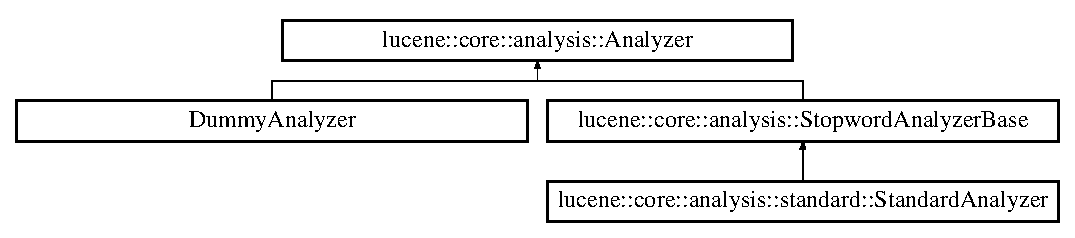
\includegraphics[height=2.754098cm]{classlucene_1_1core_1_1analysis_1_1Analyzer}
\end{center}
\end{figure}
\subsection*{Classes}
\begin{DoxyCompactItemize}
\item 
class \mbox{\hyperlink{classlucene_1_1core_1_1analysis_1_1Analyzer_1_1ReuseStrategy}{Reuse\+Strategy}}
\end{DoxyCompactItemize}
\subsection*{Public Member Functions}
\begin{DoxyCompactItemize}
\item 
\mbox{\hyperlink{classlucene_1_1core_1_1analysis_1_1Analyzer_a1be2ff17bba265bdef6e1b44748eaf96}{Analyzer}} ()
\item 
\mbox{\hyperlink{classlucene_1_1core_1_1analysis_1_1Analyzer_ae9dc5c7b575e336b14185cf403003bba}{Analyzer}} (\mbox{\hyperlink{classlucene_1_1core_1_1analysis_1_1Analyzer_1_1ReuseStrategy}{Reuse\+Strategy}} $\ast$\mbox{\hyperlink{classlucene_1_1core_1_1analysis_1_1Analyzer_a8c0924436e0392015b0b3df59d35717c}{reuse\+\_\+strategy}})
\item 
virtual \mbox{\hyperlink{classlucene_1_1core_1_1analysis_1_1Analyzer_afa899ac3a6aabbe59f791f69368ad740}{$\sim$\+Analyzer}} ()
\item 
\mbox{\hyperlink{classlucene_1_1core_1_1analysis_1_1TokenStream}{Token\+Stream}} \& \mbox{\hyperlink{classlucene_1_1core_1_1analysis_1_1Analyzer_a010cdb318b51c27c46b8cbf5a1cfe20e}{Get\+Token\+Stream}} (const std\+::string \&field\+\_\+name, \mbox{\hyperlink{classlucene_1_1core_1_1analysis_1_1Reader}{Reader}} \&reader)
\item 
\mbox{\hyperlink{classlucene_1_1core_1_1analysis_1_1TokenStream}{Token\+Stream}} \& \mbox{\hyperlink{classlucene_1_1core_1_1analysis_1_1Analyzer_a385dbda39ff79997402b35ddbb296697}{Get\+Token\+Stream}} (const std\+::string \&field\+\_\+name, const std\+::string \&text)
\item 
\mbox{\hyperlink{classlucene_1_1core_1_1util_1_1BytesRef}{lucene\+::core\+::util\+::\+Bytes\+Ref}} \mbox{\hyperlink{classlucene_1_1core_1_1analysis_1_1Analyzer_aff90a96fce2aa5ab99c6c2a880849812}{Normalize}} (const std\+::string \&field\+\_\+name, const std\+::string \&text)
\item 
uint32\+\_\+t \mbox{\hyperlink{classlucene_1_1core_1_1analysis_1_1Analyzer_a97cced949f5cfd3e4527b82fc178fa42}{Get\+Position\+Increment\+Gap}} (const std\+::string \&field\+\_\+name) const
\item 
uint32\+\_\+t \mbox{\hyperlink{classlucene_1_1core_1_1analysis_1_1Analyzer_af535ad197952fbf88c74e4298bb6a9f1}{Get\+Offset\+Gap}} (const std\+::string \&field\+\_\+name) const
\item 
\mbox{\hyperlink{classlucene_1_1core_1_1analysis_1_1Analyzer_1_1ReuseStrategy}{Reuse\+Strategy}} \& \mbox{\hyperlink{classlucene_1_1core_1_1analysis_1_1Analyzer_afbf37ccc45ae5a78ef6f9399ac484c64}{Get\+Reuse\+Strategy}} ()
\item 
void \mbox{\hyperlink{classlucene_1_1core_1_1analysis_1_1Analyzer_a9c0504cdb7f9e1fc8e4815505ce55683}{Set\+Version}} (\mbox{\hyperlink{classlucene_1_1core_1_1util_1_1etc_1_1Version}{lucene\+::core\+::util\+::etc\+::\+Version}} \&v)
\item 
const \mbox{\hyperlink{classlucene_1_1core_1_1util_1_1etc_1_1Version}{lucene\+::core\+::util\+::etc\+::\+Version}} \& \mbox{\hyperlink{classlucene_1_1core_1_1analysis_1_1Analyzer_a1679f175b96b88508c148f6d8872623d}{Get\+Version}} () const
\item 
void \mbox{\hyperlink{classlucene_1_1core_1_1analysis_1_1Analyzer_a5c80fc8a7e06ebd552d9d4e42d7466ad}{Close}} () noexcept
\item 
bool \mbox{\hyperlink{classlucene_1_1core_1_1analysis_1_1Analyzer_a3a533567be4805332be57160b0364b79}{Is\+Closed}} () const noexcept
\end{DoxyCompactItemize}
\subsection*{Protected Member Functions}
\begin{DoxyCompactItemize}
\item 
virtual \mbox{\hyperlink{classlucene_1_1core_1_1analysis_1_1TokenStreamComponents}{Token\+Stream\+Components}} $\ast$ \mbox{\hyperlink{classlucene_1_1core_1_1analysis_1_1Analyzer_a9b7dc3c598057fbf4e9b5f48066cb54a}{Create\+Components}} (const std\+::string \&field\+\_\+name)=0
\item 
virtual \mbox{\hyperlink{classlucene_1_1core_1_1analysis_1_1Reader}{Reader}} \& \mbox{\hyperlink{classlucene_1_1core_1_1analysis_1_1Analyzer_aed8b22b06eab4ecd4f3d568cadab8b09}{Init\+Reader}} (const std\+::string \&field\+\_\+name, \mbox{\hyperlink{classlucene_1_1core_1_1analysis_1_1Reader}{Reader}} \&reader)
\item 
\mbox{\hyperlink{classlucene_1_1core_1_1analysis_1_1TokenStream}{Token\+Stream}} \& \mbox{\hyperlink{classlucene_1_1core_1_1analysis_1_1Analyzer_a9c76b9071c95ee8347b0f8ae2a208e6e}{Normalize}} (const std\+::string \&field\+\_\+name, \mbox{\hyperlink{classlucene_1_1core_1_1analysis_1_1TokenStream}{Token\+Stream}} \&in)
\item 
\mbox{\hyperlink{classlucene_1_1core_1_1analysis_1_1Reader}{Reader}} \& \mbox{\hyperlink{classlucene_1_1core_1_1analysis_1_1Analyzer_ae261718804348d65059b44feb6349496}{Init\+Reader\+For\+Normalization}} (const std\+::string \&field\+\_\+name, \mbox{\hyperlink{classlucene_1_1core_1_1analysis_1_1Reader}{Reader}} \&reader)
\item 
\mbox{\hyperlink{classlucene_1_1core_1_1util_1_1AttributeFactory}{lucene\+::core\+::util\+::\+Attribute\+Factory}} \& \mbox{\hyperlink{classlucene_1_1core_1_1analysis_1_1Analyzer_af0c3e02aef0e7a391b0abdbca218951b}{Get\+Attribute\+Factory}} (const std\+::string \&field\+\_\+name)
\end{DoxyCompactItemize}
\subsection*{Private Attributes}
\begin{DoxyCompactItemize}
\item 
bool \mbox{\hyperlink{classlucene_1_1core_1_1analysis_1_1Analyzer_a869f08194af89da7f8c68e211d73607c}{closed}}
\item 
std\+::unique\+\_\+ptr$<$ \mbox{\hyperlink{classlucene_1_1core_1_1analysis_1_1Analyzer_1_1ReuseStrategy}{Reuse\+Strategy}} $>$ \mbox{\hyperlink{classlucene_1_1core_1_1analysis_1_1Analyzer_a8c0924436e0392015b0b3df59d35717c}{reuse\+\_\+strategy}}
\item 
\mbox{\hyperlink{classlucene_1_1core_1_1util_1_1etc_1_1Version}{lucene\+::core\+::util\+::etc\+::\+Version}} \mbox{\hyperlink{classlucene_1_1core_1_1analysis_1_1Analyzer_ac04041d68279aa308509d8e8cfcf89e1}{version}}
\end{DoxyCompactItemize}


\subsection{Constructor \& Destructor Documentation}
\mbox{\Hypertarget{classlucene_1_1core_1_1analysis_1_1Analyzer_a1be2ff17bba265bdef6e1b44748eaf96}\label{classlucene_1_1core_1_1analysis_1_1Analyzer_a1be2ff17bba265bdef6e1b44748eaf96}} 
\index{lucene\+::core\+::analysis\+::\+Analyzer@{lucene\+::core\+::analysis\+::\+Analyzer}!Analyzer@{Analyzer}}
\index{Analyzer@{Analyzer}!lucene\+::core\+::analysis\+::\+Analyzer@{lucene\+::core\+::analysis\+::\+Analyzer}}
\subsubsection{\texorpdfstring{Analyzer()}{Analyzer()}\hspace{0.1cm}{\footnotesize\ttfamily [1/2]}}
{\footnotesize\ttfamily Analyzer\+::\+Analyzer (\begin{DoxyParamCaption}{ }\end{DoxyParamCaption})}

\mbox{\hyperlink{classlucene_1_1core_1_1analysis_1_1Analyzer}{Analyzer}} \mbox{\Hypertarget{classlucene_1_1core_1_1analysis_1_1Analyzer_ae9dc5c7b575e336b14185cf403003bba}\label{classlucene_1_1core_1_1analysis_1_1Analyzer_ae9dc5c7b575e336b14185cf403003bba}} 
\index{lucene\+::core\+::analysis\+::\+Analyzer@{lucene\+::core\+::analysis\+::\+Analyzer}!Analyzer@{Analyzer}}
\index{Analyzer@{Analyzer}!lucene\+::core\+::analysis\+::\+Analyzer@{lucene\+::core\+::analysis\+::\+Analyzer}}
\subsubsection{\texorpdfstring{Analyzer()}{Analyzer()}\hspace{0.1cm}{\footnotesize\ttfamily [2/2]}}
{\footnotesize\ttfamily Analyzer\+::\+Analyzer (\begin{DoxyParamCaption}\item[{\mbox{\hyperlink{classlucene_1_1core_1_1analysis_1_1Analyzer_1_1ReuseStrategy}{Reuse\+Strategy}} $\ast$}]{reuse\+\_\+strategy }\end{DoxyParamCaption})\hspace{0.3cm}{\ttfamily [explicit]}}

\mbox{\Hypertarget{classlucene_1_1core_1_1analysis_1_1Analyzer_afa899ac3a6aabbe59f791f69368ad740}\label{classlucene_1_1core_1_1analysis_1_1Analyzer_afa899ac3a6aabbe59f791f69368ad740}} 
\index{lucene\+::core\+::analysis\+::\+Analyzer@{lucene\+::core\+::analysis\+::\+Analyzer}!````~Analyzer@{$\sim$\+Analyzer}}
\index{````~Analyzer@{$\sim$\+Analyzer}!lucene\+::core\+::analysis\+::\+Analyzer@{lucene\+::core\+::analysis\+::\+Analyzer}}
\subsubsection{\texorpdfstring{$\sim$\+Analyzer()}{~Analyzer()}}
{\footnotesize\ttfamily Analyzer\+::$\sim$\+Analyzer (\begin{DoxyParamCaption}{ }\end{DoxyParamCaption})\hspace{0.3cm}{\ttfamily [virtual]}}



\subsection{Member Function Documentation}
\mbox{\Hypertarget{classlucene_1_1core_1_1analysis_1_1Analyzer_a5c80fc8a7e06ebd552d9d4e42d7466ad}\label{classlucene_1_1core_1_1analysis_1_1Analyzer_a5c80fc8a7e06ebd552d9d4e42d7466ad}} 
\index{lucene\+::core\+::analysis\+::\+Analyzer@{lucene\+::core\+::analysis\+::\+Analyzer}!Close@{Close}}
\index{Close@{Close}!lucene\+::core\+::analysis\+::\+Analyzer@{lucene\+::core\+::analysis\+::\+Analyzer}}
\subsubsection{\texorpdfstring{Close()}{Close()}}
{\footnotesize\ttfamily void lucene\+::core\+::analysis\+::\+Analyzer\+::\+Close (\begin{DoxyParamCaption}{ }\end{DoxyParamCaption})\hspace{0.3cm}{\ttfamily [inline]}, {\ttfamily [noexcept]}}

\mbox{\Hypertarget{classlucene_1_1core_1_1analysis_1_1Analyzer_a9b7dc3c598057fbf4e9b5f48066cb54a}\label{classlucene_1_1core_1_1analysis_1_1Analyzer_a9b7dc3c598057fbf4e9b5f48066cb54a}} 
\index{lucene\+::core\+::analysis\+::\+Analyzer@{lucene\+::core\+::analysis\+::\+Analyzer}!Create\+Components@{Create\+Components}}
\index{Create\+Components@{Create\+Components}!lucene\+::core\+::analysis\+::\+Analyzer@{lucene\+::core\+::analysis\+::\+Analyzer}}
\subsubsection{\texorpdfstring{Create\+Components()}{CreateComponents()}}
{\footnotesize\ttfamily virtual \mbox{\hyperlink{classlucene_1_1core_1_1analysis_1_1TokenStreamComponents}{Token\+Stream\+Components}}$\ast$ lucene\+::core\+::analysis\+::\+Analyzer\+::\+Create\+Components (\begin{DoxyParamCaption}\item[{const std\+::string \&}]{field\+\_\+name }\end{DoxyParamCaption})\hspace{0.3cm}{\ttfamily [protected]}, {\ttfamily [pure virtual]}}



Implemented in \mbox{\hyperlink{classDummyAnalyzer_aeeb24aa6449d4bf7c4adc6a5c63a5c0e}{Dummy\+Analyzer}}, and \mbox{\hyperlink{classlucene_1_1core_1_1analysis_1_1standard_1_1StandardAnalyzer_a0d569e3e48f2060a4698481ec1b49d12}{lucene\+::core\+::analysis\+::standard\+::\+Standard\+Analyzer}}.

\mbox{\Hypertarget{classlucene_1_1core_1_1analysis_1_1Analyzer_af0c3e02aef0e7a391b0abdbca218951b}\label{classlucene_1_1core_1_1analysis_1_1Analyzer_af0c3e02aef0e7a391b0abdbca218951b}} 
\index{lucene\+::core\+::analysis\+::\+Analyzer@{lucene\+::core\+::analysis\+::\+Analyzer}!Get\+Attribute\+Factory@{Get\+Attribute\+Factory}}
\index{Get\+Attribute\+Factory@{Get\+Attribute\+Factory}!lucene\+::core\+::analysis\+::\+Analyzer@{lucene\+::core\+::analysis\+::\+Analyzer}}
\subsubsection{\texorpdfstring{Get\+Attribute\+Factory()}{GetAttributeFactory()}}
{\footnotesize\ttfamily \mbox{\hyperlink{classlucene_1_1core_1_1util_1_1AttributeFactory}{Attribute\+Factory}} \& Analyzer\+::\+Get\+Attribute\+Factory (\begin{DoxyParamCaption}\item[{const std\+::string \&}]{field\+\_\+name }\end{DoxyParamCaption})\hspace{0.3cm}{\ttfamily [protected]}}

\mbox{\Hypertarget{classlucene_1_1core_1_1analysis_1_1Analyzer_af535ad197952fbf88c74e4298bb6a9f1}\label{classlucene_1_1core_1_1analysis_1_1Analyzer_af535ad197952fbf88c74e4298bb6a9f1}} 
\index{lucene\+::core\+::analysis\+::\+Analyzer@{lucene\+::core\+::analysis\+::\+Analyzer}!Get\+Offset\+Gap@{Get\+Offset\+Gap}}
\index{Get\+Offset\+Gap@{Get\+Offset\+Gap}!lucene\+::core\+::analysis\+::\+Analyzer@{lucene\+::core\+::analysis\+::\+Analyzer}}
\subsubsection{\texorpdfstring{Get\+Offset\+Gap()}{GetOffsetGap()}}
{\footnotesize\ttfamily uint32\+\_\+t lucene\+::core\+::analysis\+::\+Analyzer\+::\+Get\+Offset\+Gap (\begin{DoxyParamCaption}\item[{const std\+::string \&}]{field\+\_\+name }\end{DoxyParamCaption}) const\hspace{0.3cm}{\ttfamily [inline]}}

\mbox{\Hypertarget{classlucene_1_1core_1_1analysis_1_1Analyzer_a97cced949f5cfd3e4527b82fc178fa42}\label{classlucene_1_1core_1_1analysis_1_1Analyzer_a97cced949f5cfd3e4527b82fc178fa42}} 
\index{lucene\+::core\+::analysis\+::\+Analyzer@{lucene\+::core\+::analysis\+::\+Analyzer}!Get\+Position\+Increment\+Gap@{Get\+Position\+Increment\+Gap}}
\index{Get\+Position\+Increment\+Gap@{Get\+Position\+Increment\+Gap}!lucene\+::core\+::analysis\+::\+Analyzer@{lucene\+::core\+::analysis\+::\+Analyzer}}
\subsubsection{\texorpdfstring{Get\+Position\+Increment\+Gap()}{GetPositionIncrementGap()}}
{\footnotesize\ttfamily uint32\+\_\+t lucene\+::core\+::analysis\+::\+Analyzer\+::\+Get\+Position\+Increment\+Gap (\begin{DoxyParamCaption}\item[{const std\+::string \&}]{field\+\_\+name }\end{DoxyParamCaption}) const\hspace{0.3cm}{\ttfamily [inline]}}

\mbox{\Hypertarget{classlucene_1_1core_1_1analysis_1_1Analyzer_afbf37ccc45ae5a78ef6f9399ac484c64}\label{classlucene_1_1core_1_1analysis_1_1Analyzer_afbf37ccc45ae5a78ef6f9399ac484c64}} 
\index{lucene\+::core\+::analysis\+::\+Analyzer@{lucene\+::core\+::analysis\+::\+Analyzer}!Get\+Reuse\+Strategy@{Get\+Reuse\+Strategy}}
\index{Get\+Reuse\+Strategy@{Get\+Reuse\+Strategy}!lucene\+::core\+::analysis\+::\+Analyzer@{lucene\+::core\+::analysis\+::\+Analyzer}}
\subsubsection{\texorpdfstring{Get\+Reuse\+Strategy()}{GetReuseStrategy()}}
{\footnotesize\ttfamily \mbox{\hyperlink{classlucene_1_1core_1_1analysis_1_1Analyzer_1_1ReuseStrategy}{Reuse\+Strategy}}\& lucene\+::core\+::analysis\+::\+Analyzer\+::\+Get\+Reuse\+Strategy (\begin{DoxyParamCaption}{ }\end{DoxyParamCaption})}

\mbox{\Hypertarget{classlucene_1_1core_1_1analysis_1_1Analyzer_a010cdb318b51c27c46b8cbf5a1cfe20e}\label{classlucene_1_1core_1_1analysis_1_1Analyzer_a010cdb318b51c27c46b8cbf5a1cfe20e}} 
\index{lucene\+::core\+::analysis\+::\+Analyzer@{lucene\+::core\+::analysis\+::\+Analyzer}!Get\+Token\+Stream@{Get\+Token\+Stream}}
\index{Get\+Token\+Stream@{Get\+Token\+Stream}!lucene\+::core\+::analysis\+::\+Analyzer@{lucene\+::core\+::analysis\+::\+Analyzer}}
\subsubsection{\texorpdfstring{Get\+Token\+Stream()}{GetTokenStream()}\hspace{0.1cm}{\footnotesize\ttfamily [1/2]}}
{\footnotesize\ttfamily \mbox{\hyperlink{classlucene_1_1core_1_1analysis_1_1TokenStream}{Token\+Stream}} \& Analyzer\+::\+Get\+Token\+Stream (\begin{DoxyParamCaption}\item[{const std\+::string \&}]{field\+\_\+name,  }\item[{\mbox{\hyperlink{classlucene_1_1core_1_1analysis_1_1Reader}{Reader}} \&}]{reader }\end{DoxyParamCaption})}

\mbox{\Hypertarget{classlucene_1_1core_1_1analysis_1_1Analyzer_a385dbda39ff79997402b35ddbb296697}\label{classlucene_1_1core_1_1analysis_1_1Analyzer_a385dbda39ff79997402b35ddbb296697}} 
\index{lucene\+::core\+::analysis\+::\+Analyzer@{lucene\+::core\+::analysis\+::\+Analyzer}!Get\+Token\+Stream@{Get\+Token\+Stream}}
\index{Get\+Token\+Stream@{Get\+Token\+Stream}!lucene\+::core\+::analysis\+::\+Analyzer@{lucene\+::core\+::analysis\+::\+Analyzer}}
\subsubsection{\texorpdfstring{Get\+Token\+Stream()}{GetTokenStream()}\hspace{0.1cm}{\footnotesize\ttfamily [2/2]}}
{\footnotesize\ttfamily \mbox{\hyperlink{classlucene_1_1core_1_1analysis_1_1TokenStream}{Token\+Stream}} \& Analyzer\+::\+Get\+Token\+Stream (\begin{DoxyParamCaption}\item[{const std\+::string \&}]{field\+\_\+name,  }\item[{const std\+::string \&}]{text }\end{DoxyParamCaption})}

\mbox{\Hypertarget{classlucene_1_1core_1_1analysis_1_1Analyzer_a1679f175b96b88508c148f6d8872623d}\label{classlucene_1_1core_1_1analysis_1_1Analyzer_a1679f175b96b88508c148f6d8872623d}} 
\index{lucene\+::core\+::analysis\+::\+Analyzer@{lucene\+::core\+::analysis\+::\+Analyzer}!Get\+Version@{Get\+Version}}
\index{Get\+Version@{Get\+Version}!lucene\+::core\+::analysis\+::\+Analyzer@{lucene\+::core\+::analysis\+::\+Analyzer}}
\subsubsection{\texorpdfstring{Get\+Version()}{GetVersion()}}
{\footnotesize\ttfamily const \mbox{\hyperlink{classlucene_1_1core_1_1util_1_1etc_1_1Version}{lucene\+::core\+::util\+::etc\+::\+Version}}\& lucene\+::core\+::analysis\+::\+Analyzer\+::\+Get\+Version (\begin{DoxyParamCaption}{ }\end{DoxyParamCaption}) const\hspace{0.3cm}{\ttfamily [inline]}}

\mbox{\Hypertarget{classlucene_1_1core_1_1analysis_1_1Analyzer_aed8b22b06eab4ecd4f3d568cadab8b09}\label{classlucene_1_1core_1_1analysis_1_1Analyzer_aed8b22b06eab4ecd4f3d568cadab8b09}} 
\index{lucene\+::core\+::analysis\+::\+Analyzer@{lucene\+::core\+::analysis\+::\+Analyzer}!Init\+Reader@{Init\+Reader}}
\index{Init\+Reader@{Init\+Reader}!lucene\+::core\+::analysis\+::\+Analyzer@{lucene\+::core\+::analysis\+::\+Analyzer}}
\subsubsection{\texorpdfstring{Init\+Reader()}{InitReader()}}
{\footnotesize\ttfamily \mbox{\hyperlink{classlucene_1_1core_1_1analysis_1_1Reader}{Reader}} \& Analyzer\+::\+Init\+Reader (\begin{DoxyParamCaption}\item[{const std\+::string \&}]{field\+\_\+name,  }\item[{\mbox{\hyperlink{classlucene_1_1core_1_1analysis_1_1Reader}{Reader}} \&}]{reader }\end{DoxyParamCaption})\hspace{0.3cm}{\ttfamily [protected]}, {\ttfamily [virtual]}}

\mbox{\Hypertarget{classlucene_1_1core_1_1analysis_1_1Analyzer_ae261718804348d65059b44feb6349496}\label{classlucene_1_1core_1_1analysis_1_1Analyzer_ae261718804348d65059b44feb6349496}} 
\index{lucene\+::core\+::analysis\+::\+Analyzer@{lucene\+::core\+::analysis\+::\+Analyzer}!Init\+Reader\+For\+Normalization@{Init\+Reader\+For\+Normalization}}
\index{Init\+Reader\+For\+Normalization@{Init\+Reader\+For\+Normalization}!lucene\+::core\+::analysis\+::\+Analyzer@{lucene\+::core\+::analysis\+::\+Analyzer}}
\subsubsection{\texorpdfstring{Init\+Reader\+For\+Normalization()}{InitReaderForNormalization()}}
{\footnotesize\ttfamily \mbox{\hyperlink{classlucene_1_1core_1_1analysis_1_1Reader}{Reader}} \& Analyzer\+::\+Init\+Reader\+For\+Normalization (\begin{DoxyParamCaption}\item[{const std\+::string \&}]{field\+\_\+name,  }\item[{\mbox{\hyperlink{classlucene_1_1core_1_1analysis_1_1Reader}{Reader}} \&}]{reader }\end{DoxyParamCaption})\hspace{0.3cm}{\ttfamily [protected]}}

\mbox{\Hypertarget{classlucene_1_1core_1_1analysis_1_1Analyzer_a3a533567be4805332be57160b0364b79}\label{classlucene_1_1core_1_1analysis_1_1Analyzer_a3a533567be4805332be57160b0364b79}} 
\index{lucene\+::core\+::analysis\+::\+Analyzer@{lucene\+::core\+::analysis\+::\+Analyzer}!Is\+Closed@{Is\+Closed}}
\index{Is\+Closed@{Is\+Closed}!lucene\+::core\+::analysis\+::\+Analyzer@{lucene\+::core\+::analysis\+::\+Analyzer}}
\subsubsection{\texorpdfstring{Is\+Closed()}{IsClosed()}}
{\footnotesize\ttfamily bool lucene\+::core\+::analysis\+::\+Analyzer\+::\+Is\+Closed (\begin{DoxyParamCaption}{ }\end{DoxyParamCaption}) const\hspace{0.3cm}{\ttfamily [inline]}, {\ttfamily [noexcept]}}

\mbox{\Hypertarget{classlucene_1_1core_1_1analysis_1_1Analyzer_a9c76b9071c95ee8347b0f8ae2a208e6e}\label{classlucene_1_1core_1_1analysis_1_1Analyzer_a9c76b9071c95ee8347b0f8ae2a208e6e}} 
\index{lucene\+::core\+::analysis\+::\+Analyzer@{lucene\+::core\+::analysis\+::\+Analyzer}!Normalize@{Normalize}}
\index{Normalize@{Normalize}!lucene\+::core\+::analysis\+::\+Analyzer@{lucene\+::core\+::analysis\+::\+Analyzer}}
\subsubsection{\texorpdfstring{Normalize()}{Normalize()}\hspace{0.1cm}{\footnotesize\ttfamily [1/2]}}
{\footnotesize\ttfamily \mbox{\hyperlink{classlucene_1_1core_1_1analysis_1_1TokenStream}{Token\+Stream}} \& Analyzer\+::\+Normalize (\begin{DoxyParamCaption}\item[{const std\+::string \&}]{field\+\_\+name,  }\item[{\mbox{\hyperlink{classlucene_1_1core_1_1analysis_1_1TokenStream}{Token\+Stream}} \&}]{in }\end{DoxyParamCaption})\hspace{0.3cm}{\ttfamily [protected]}}

\mbox{\Hypertarget{classlucene_1_1core_1_1analysis_1_1Analyzer_aff90a96fce2aa5ab99c6c2a880849812}\label{classlucene_1_1core_1_1analysis_1_1Analyzer_aff90a96fce2aa5ab99c6c2a880849812}} 
\index{lucene\+::core\+::analysis\+::\+Analyzer@{lucene\+::core\+::analysis\+::\+Analyzer}!Normalize@{Normalize}}
\index{Normalize@{Normalize}!lucene\+::core\+::analysis\+::\+Analyzer@{lucene\+::core\+::analysis\+::\+Analyzer}}
\subsubsection{\texorpdfstring{Normalize()}{Normalize()}\hspace{0.1cm}{\footnotesize\ttfamily [2/2]}}
{\footnotesize\ttfamily \mbox{\hyperlink{classlucene_1_1core_1_1util_1_1BytesRef}{Bytes\+Ref}} Analyzer\+::\+Normalize (\begin{DoxyParamCaption}\item[{const std\+::string \&}]{field\+\_\+name,  }\item[{const std\+::string \&}]{text }\end{DoxyParamCaption})}

\mbox{\Hypertarget{classlucene_1_1core_1_1analysis_1_1Analyzer_a9c0504cdb7f9e1fc8e4815505ce55683}\label{classlucene_1_1core_1_1analysis_1_1Analyzer_a9c0504cdb7f9e1fc8e4815505ce55683}} 
\index{lucene\+::core\+::analysis\+::\+Analyzer@{lucene\+::core\+::analysis\+::\+Analyzer}!Set\+Version@{Set\+Version}}
\index{Set\+Version@{Set\+Version}!lucene\+::core\+::analysis\+::\+Analyzer@{lucene\+::core\+::analysis\+::\+Analyzer}}
\subsubsection{\texorpdfstring{Set\+Version()}{SetVersion()}}
{\footnotesize\ttfamily void lucene\+::core\+::analysis\+::\+Analyzer\+::\+Set\+Version (\begin{DoxyParamCaption}\item[{\mbox{\hyperlink{classlucene_1_1core_1_1util_1_1etc_1_1Version}{lucene\+::core\+::util\+::etc\+::\+Version}} \&}]{v }\end{DoxyParamCaption})\hspace{0.3cm}{\ttfamily [inline]}}



\subsection{Member Data Documentation}
\mbox{\Hypertarget{classlucene_1_1core_1_1analysis_1_1Analyzer_a869f08194af89da7f8c68e211d73607c}\label{classlucene_1_1core_1_1analysis_1_1Analyzer_a869f08194af89da7f8c68e211d73607c}} 
\index{lucene\+::core\+::analysis\+::\+Analyzer@{lucene\+::core\+::analysis\+::\+Analyzer}!closed@{closed}}
\index{closed@{closed}!lucene\+::core\+::analysis\+::\+Analyzer@{lucene\+::core\+::analysis\+::\+Analyzer}}
\subsubsection{\texorpdfstring{closed}{closed}}
{\footnotesize\ttfamily bool lucene\+::core\+::analysis\+::\+Analyzer\+::closed\hspace{0.3cm}{\ttfamily [private]}}

\mbox{\Hypertarget{classlucene_1_1core_1_1analysis_1_1Analyzer_a8c0924436e0392015b0b3df59d35717c}\label{classlucene_1_1core_1_1analysis_1_1Analyzer_a8c0924436e0392015b0b3df59d35717c}} 
\index{lucene\+::core\+::analysis\+::\+Analyzer@{lucene\+::core\+::analysis\+::\+Analyzer}!reuse\+\_\+strategy@{reuse\+\_\+strategy}}
\index{reuse\+\_\+strategy@{reuse\+\_\+strategy}!lucene\+::core\+::analysis\+::\+Analyzer@{lucene\+::core\+::analysis\+::\+Analyzer}}
\subsubsection{\texorpdfstring{reuse\+\_\+strategy}{reuse\_strategy}}
{\footnotesize\ttfamily std\+::unique\+\_\+ptr$<$\mbox{\hyperlink{classlucene_1_1core_1_1analysis_1_1Analyzer_1_1ReuseStrategy}{Reuse\+Strategy}}$>$ lucene\+::core\+::analysis\+::\+Analyzer\+::reuse\+\_\+strategy\hspace{0.3cm}{\ttfamily [private]}}

\mbox{\Hypertarget{classlucene_1_1core_1_1analysis_1_1Analyzer_ac04041d68279aa308509d8e8cfcf89e1}\label{classlucene_1_1core_1_1analysis_1_1Analyzer_ac04041d68279aa308509d8e8cfcf89e1}} 
\index{lucene\+::core\+::analysis\+::\+Analyzer@{lucene\+::core\+::analysis\+::\+Analyzer}!version@{version}}
\index{version@{version}!lucene\+::core\+::analysis\+::\+Analyzer@{lucene\+::core\+::analysis\+::\+Analyzer}}
\subsubsection{\texorpdfstring{version}{version}}
{\footnotesize\ttfamily \mbox{\hyperlink{classlucene_1_1core_1_1util_1_1etc_1_1Version}{lucene\+::core\+::util\+::etc\+::\+Version}} lucene\+::core\+::analysis\+::\+Analyzer\+::version\hspace{0.3cm}{\ttfamily [private]}}



The documentation for this class was generated from the following files\+:\begin{DoxyCompactItemize}
\item 
Analysis/\mbox{\hyperlink{Analyzer_8h}{Analyzer.\+h}}\item 
Analysis/\mbox{\hyperlink{Analyzer_8cpp}{Analyzer.\+cpp}}\end{DoxyCompactItemize}

\hypertarget{classlucene_1_1core_1_1util_1_1Attribute}{}\section{lucene\+:\+:core\+:\+:util\+:\+:Attribute Class Reference}
\label{classlucene_1_1core_1_1util_1_1Attribute}\index{lucene\+::core\+::util\+::\+Attribute@{lucene\+::core\+::util\+::\+Attribute}}


{\ttfamily \#include $<$Attribute.\+h$>$}

Inheritance diagram for lucene\+:\+:core\+:\+:util\+:\+:Attribute\+:\begin{figure}[H]
\begin{center}
\leavevmode
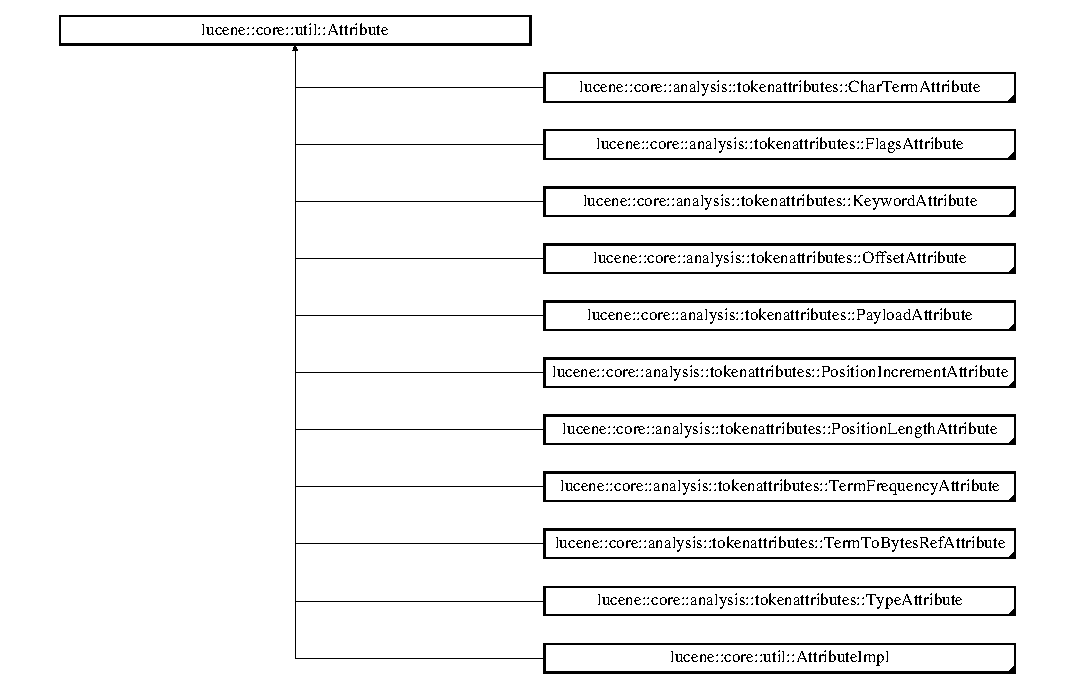
\includegraphics[height=8.818898cm]{classlucene_1_1core_1_1util_1_1Attribute}
\end{center}
\end{figure}
\subsection*{Public Member Functions}
\begin{DoxyCompactItemize}
\item 
virtual \mbox{\hyperlink{classlucene_1_1core_1_1util_1_1Attribute_aad48274d053d0ec9afd948fea76f7ce9}{$\sim$\+Attribute}} ()
\end{DoxyCompactItemize}
\subsection*{Static Public Member Functions}
\begin{DoxyCompactItemize}
\item 
{\footnotesize template$<$typename T $>$ }\\static std\+::type\+\_\+index \mbox{\hyperlink{classlucene_1_1core_1_1util_1_1Attribute_a2093d08d843c5a937fff2f3fbdb4341c}{Type\+Id}} ()
\end{DoxyCompactItemize}


\subsection{Constructor \& Destructor Documentation}
\mbox{\Hypertarget{classlucene_1_1core_1_1util_1_1Attribute_aad48274d053d0ec9afd948fea76f7ce9}\label{classlucene_1_1core_1_1util_1_1Attribute_aad48274d053d0ec9afd948fea76f7ce9}} 
\index{lucene\+::core\+::util\+::\+Attribute@{lucene\+::core\+::util\+::\+Attribute}!````~Attribute@{$\sim$\+Attribute}}
\index{````~Attribute@{$\sim$\+Attribute}!lucene\+::core\+::util\+::\+Attribute@{lucene\+::core\+::util\+::\+Attribute}}
\subsubsection{\texorpdfstring{$\sim$\+Attribute()}{~Attribute()}}
{\footnotesize\ttfamily virtual lucene\+::core\+::util\+::\+Attribute\+::$\sim$\+Attribute (\begin{DoxyParamCaption}{ }\end{DoxyParamCaption})\hspace{0.3cm}{\ttfamily [inline]}, {\ttfamily [virtual]}}



\subsection{Member Function Documentation}
\mbox{\Hypertarget{classlucene_1_1core_1_1util_1_1Attribute_a2093d08d843c5a937fff2f3fbdb4341c}\label{classlucene_1_1core_1_1util_1_1Attribute_a2093d08d843c5a937fff2f3fbdb4341c}} 
\index{lucene\+::core\+::util\+::\+Attribute@{lucene\+::core\+::util\+::\+Attribute}!Type\+Id@{Type\+Id}}
\index{Type\+Id@{Type\+Id}!lucene\+::core\+::util\+::\+Attribute@{lucene\+::core\+::util\+::\+Attribute}}
\subsubsection{\texorpdfstring{Type\+Id()}{TypeId()}}
{\footnotesize\ttfamily template$<$typename T $>$ \\
static std\+::type\+\_\+index lucene\+::core\+::util\+::\+Attribute\+::\+Type\+Id (\begin{DoxyParamCaption}{ }\end{DoxyParamCaption})\hspace{0.3cm}{\ttfamily [inline]}, {\ttfamily [static]}}



The documentation for this class was generated from the following file\+:\begin{DoxyCompactItemize}
\item 
Util/\mbox{\hyperlink{Util_2Attribute_8h}{Attribute.\+h}}\end{DoxyCompactItemize}

\hypertarget{classlucene_1_1core_1_1util_1_1AttributeFactory}{}\section{lucene\+:\+:core\+:\+:util\+:\+:Attribute\+Factory Class Reference}
\label{classlucene_1_1core_1_1util_1_1AttributeFactory}\index{lucene\+::core\+::util\+::\+Attribute\+Factory@{lucene\+::core\+::util\+::\+Attribute\+Factory}}


{\ttfamily \#include $<$Attribute.\+h$>$}

Inheritance diagram for lucene\+:\+:core\+:\+:util\+:\+:Attribute\+Factory\+:\begin{figure}[H]
\begin{center}
\leavevmode
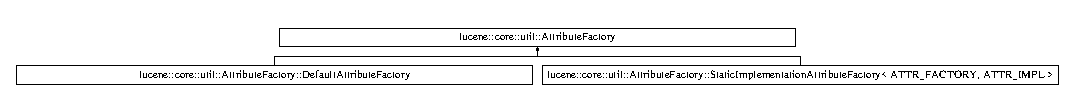
\includegraphics[height=0.907618cm]{classlucene_1_1core_1_1util_1_1AttributeFactory}
\end{center}
\end{figure}
\subsection*{Classes}
\begin{DoxyCompactItemize}
\item 
class \mbox{\hyperlink{classlucene_1_1core_1_1util_1_1AttributeFactory_1_1DefaultAttributeFactory}{Default\+Attribute\+Factory}}
\item 
class \mbox{\hyperlink{classlucene_1_1core_1_1util_1_1AttributeFactory_1_1StaticImplementationAttributeFactory}{Static\+Implementation\+Attribute\+Factory}}
\end{DoxyCompactItemize}
\subsection*{Public Member Functions}
\begin{DoxyCompactItemize}
\item 
\mbox{\hyperlink{classlucene_1_1core_1_1util_1_1AttributeFactory_a55d388271f308e3105344163e56dddc4}{Attribute\+Factory}} ()
\item 
virtual \mbox{\hyperlink{classlucene_1_1core_1_1util_1_1AttributeFactory_a0388433c20c2b44a344c2f5838060728}{$\sim$\+Attribute\+Factory}} ()
\item 
virtual \mbox{\hyperlink{classlucene_1_1core_1_1util_1_1AttributeImpl}{Attribute\+Impl}} $\ast$ \mbox{\hyperlink{classlucene_1_1core_1_1util_1_1AttributeFactory_a88ccb9965ed78099379eaf9b1256abf3}{Create\+Attribute\+Instance}} (\mbox{\hyperlink{ZlibCrc32_8h_a2c212835823e3c54a8ab6d95c652660e}{const}} std\+::type\+\_\+index attr\+\_\+type\+\_\+id)=0
\end{DoxyCompactItemize}
\subsection*{Static Public Member Functions}
\begin{DoxyCompactItemize}
\item 
static \mbox{\hyperlink{namespacelucene_1_1core_1_1util_acbd8821be7d7b29749374e57b0a7c40b}{Attribute\+Impl\+Generator}} \mbox{\hyperlink{classlucene_1_1core_1_1util_1_1AttributeFactory_af56838e41c83a10b00063e02c3f910e6}{Find\+Attribute\+Impl\+Generator}} (\mbox{\hyperlink{ZlibCrc32_8h_a2c212835823e3c54a8ab6d95c652660e}{const}} std\+::type\+\_\+index attr\+\_\+type\+\_\+id)
\item 
{\footnotesize template$<$typename A\+T\+T\+R\+\_\+\+F\+A\+C\+T\+O\+RY , typename A\+T\+T\+R\+\_\+\+I\+M\+PL $>$ }\\static \mbox{\hyperlink{classlucene_1_1core_1_1util_1_1AttributeFactory}{Attribute\+Factory}} $\ast$ \mbox{\hyperlink{classlucene_1_1core_1_1util_1_1AttributeFactory_ac770bcd808b70e6d1d5f8a3c6cd8150d}{Get\+Static\+Implementation}} ()
\item 
{\footnotesize template$<$typename A\+T\+TR , typename A\+T\+T\+R\+\_\+\+I\+M\+P\+L\+\_\+\+C\+L\+A\+SS $>$ }\\static void \mbox{\hyperlink{classlucene_1_1core_1_1util_1_1AttributeFactory_a57d5469dd678591652d59bf3db4890e1}{Register\+Attribute\+Impl}} ()
\end{DoxyCompactItemize}
\subsection*{Static Private Attributes}
\begin{DoxyCompactItemize}
\item 
static std\+::unordered\+\_\+map$<$ std\+::type\+\_\+index, \mbox{\hyperlink{namespacelucene_1_1core_1_1util_acbd8821be7d7b29749374e57b0a7c40b}{Attribute\+Impl\+Generator}} $>$ \mbox{\hyperlink{classlucene_1_1core_1_1util_1_1AttributeFactory_a5247e47d95ce30862a15e66ce2266d04}{A\+T\+T\+R\+\_\+\+I\+M\+P\+L\+\_\+\+T\+A\+B\+LE}}
\end{DoxyCompactItemize}


\subsection{Constructor \& Destructor Documentation}
\mbox{\Hypertarget{classlucene_1_1core_1_1util_1_1AttributeFactory_a55d388271f308e3105344163e56dddc4}\label{classlucene_1_1core_1_1util_1_1AttributeFactory_a55d388271f308e3105344163e56dddc4}} 
\index{lucene\+::core\+::util\+::\+Attribute\+Factory@{lucene\+::core\+::util\+::\+Attribute\+Factory}!Attribute\+Factory@{Attribute\+Factory}}
\index{Attribute\+Factory@{Attribute\+Factory}!lucene\+::core\+::util\+::\+Attribute\+Factory@{lucene\+::core\+::util\+::\+Attribute\+Factory}}
\subsubsection{\texorpdfstring{Attribute\+Factory()}{AttributeFactory()}}
{\footnotesize\ttfamily Attribute\+Factory\+::\+Attribute\+Factory (\begin{DoxyParamCaption}{ }\end{DoxyParamCaption})}

\mbox{\Hypertarget{classlucene_1_1core_1_1util_1_1AttributeFactory_a0388433c20c2b44a344c2f5838060728}\label{classlucene_1_1core_1_1util_1_1AttributeFactory_a0388433c20c2b44a344c2f5838060728}} 
\index{lucene\+::core\+::util\+::\+Attribute\+Factory@{lucene\+::core\+::util\+::\+Attribute\+Factory}!````~Attribute\+Factory@{$\sim$\+Attribute\+Factory}}
\index{````~Attribute\+Factory@{$\sim$\+Attribute\+Factory}!lucene\+::core\+::util\+::\+Attribute\+Factory@{lucene\+::core\+::util\+::\+Attribute\+Factory}}
\subsubsection{\texorpdfstring{$\sim$\+Attribute\+Factory()}{~AttributeFactory()}}
{\footnotesize\ttfamily virtual lucene\+::core\+::util\+::\+Attribute\+Factory\+::$\sim$\+Attribute\+Factory (\begin{DoxyParamCaption}{ }\end{DoxyParamCaption})\hspace{0.3cm}{\ttfamily [inline]}, {\ttfamily [virtual]}}



\subsection{Member Function Documentation}
\mbox{\Hypertarget{classlucene_1_1core_1_1util_1_1AttributeFactory_a88ccb9965ed78099379eaf9b1256abf3}\label{classlucene_1_1core_1_1util_1_1AttributeFactory_a88ccb9965ed78099379eaf9b1256abf3}} 
\index{lucene\+::core\+::util\+::\+Attribute\+Factory@{lucene\+::core\+::util\+::\+Attribute\+Factory}!Create\+Attribute\+Instance@{Create\+Attribute\+Instance}}
\index{Create\+Attribute\+Instance@{Create\+Attribute\+Instance}!lucene\+::core\+::util\+::\+Attribute\+Factory@{lucene\+::core\+::util\+::\+Attribute\+Factory}}
\subsubsection{\texorpdfstring{Create\+Attribute\+Instance()}{CreateAttributeInstance()}}
{\footnotesize\ttfamily virtual \mbox{\hyperlink{classlucene_1_1core_1_1util_1_1AttributeImpl}{Attribute\+Impl}}$\ast$ lucene\+::core\+::util\+::\+Attribute\+Factory\+::\+Create\+Attribute\+Instance (\begin{DoxyParamCaption}\item[{\mbox{\hyperlink{ZlibCrc32_8h_a2c212835823e3c54a8ab6d95c652660e}{const}} std\+::type\+\_\+index}]{attr\+\_\+type\+\_\+id }\end{DoxyParamCaption})\hspace{0.3cm}{\ttfamily [pure virtual]}}



Implemented in \mbox{\hyperlink{classlucene_1_1core_1_1util_1_1AttributeFactory_1_1StaticImplementationAttributeFactory_a06466469f2cf37e0ef599e617d415c6a}{lucene\+::core\+::util\+::\+Attribute\+Factory\+::\+Static\+Implementation\+Attribute\+Factory$<$ A\+T\+T\+R\+\_\+\+F\+A\+C\+T\+O\+R\+Y, A\+T\+T\+R\+\_\+\+I\+M\+P\+L $>$}}, and \mbox{\hyperlink{classlucene_1_1core_1_1util_1_1AttributeFactory_1_1DefaultAttributeFactory_af9b68def67fc7995d2c5e9f3d1560f5e}{lucene\+::core\+::util\+::\+Attribute\+Factory\+::\+Default\+Attribute\+Factory}}.

\mbox{\Hypertarget{classlucene_1_1core_1_1util_1_1AttributeFactory_af56838e41c83a10b00063e02c3f910e6}\label{classlucene_1_1core_1_1util_1_1AttributeFactory_af56838e41c83a10b00063e02c3f910e6}} 
\index{lucene\+::core\+::util\+::\+Attribute\+Factory@{lucene\+::core\+::util\+::\+Attribute\+Factory}!Find\+Attribute\+Impl\+Generator@{Find\+Attribute\+Impl\+Generator}}
\index{Find\+Attribute\+Impl\+Generator@{Find\+Attribute\+Impl\+Generator}!lucene\+::core\+::util\+::\+Attribute\+Factory@{lucene\+::core\+::util\+::\+Attribute\+Factory}}
\subsubsection{\texorpdfstring{Find\+Attribute\+Impl\+Generator()}{FindAttributeImplGenerator()}}
{\footnotesize\ttfamily \mbox{\hyperlink{namespacelucene_1_1core_1_1util_acbd8821be7d7b29749374e57b0a7c40b}{Attribute\+Impl\+Generator}} Attribute\+Factory\+::\+Find\+Attribute\+Impl\+Generator (\begin{DoxyParamCaption}\item[{\mbox{\hyperlink{ZlibCrc32_8h_a2c212835823e3c54a8ab6d95c652660e}{const}} std\+::type\+\_\+index}]{attr\+\_\+type\+\_\+id }\end{DoxyParamCaption})\hspace{0.3cm}{\ttfamily [static]}}

\mbox{\Hypertarget{classlucene_1_1core_1_1util_1_1AttributeFactory_ac770bcd808b70e6d1d5f8a3c6cd8150d}\label{classlucene_1_1core_1_1util_1_1AttributeFactory_ac770bcd808b70e6d1d5f8a3c6cd8150d}} 
\index{lucene\+::core\+::util\+::\+Attribute\+Factory@{lucene\+::core\+::util\+::\+Attribute\+Factory}!Get\+Static\+Implementation@{Get\+Static\+Implementation}}
\index{Get\+Static\+Implementation@{Get\+Static\+Implementation}!lucene\+::core\+::util\+::\+Attribute\+Factory@{lucene\+::core\+::util\+::\+Attribute\+Factory}}
\subsubsection{\texorpdfstring{Get\+Static\+Implementation()}{GetStaticImplementation()}}
{\footnotesize\ttfamily template$<$typename A\+T\+T\+R\+\_\+\+F\+A\+C\+T\+O\+RY , typename A\+T\+T\+R\+\_\+\+I\+M\+PL $>$ \\
static \mbox{\hyperlink{classlucene_1_1core_1_1util_1_1AttributeFactory}{Attribute\+Factory}}$\ast$ lucene\+::core\+::util\+::\+Attribute\+Factory\+::\+Get\+Static\+Implementation (\begin{DoxyParamCaption}{ }\end{DoxyParamCaption})\hspace{0.3cm}{\ttfamily [inline]}, {\ttfamily [static]}}

\mbox{\Hypertarget{classlucene_1_1core_1_1util_1_1AttributeFactory_a57d5469dd678591652d59bf3db4890e1}\label{classlucene_1_1core_1_1util_1_1AttributeFactory_a57d5469dd678591652d59bf3db4890e1}} 
\index{lucene\+::core\+::util\+::\+Attribute\+Factory@{lucene\+::core\+::util\+::\+Attribute\+Factory}!Register\+Attribute\+Impl@{Register\+Attribute\+Impl}}
\index{Register\+Attribute\+Impl@{Register\+Attribute\+Impl}!lucene\+::core\+::util\+::\+Attribute\+Factory@{lucene\+::core\+::util\+::\+Attribute\+Factory}}
\subsubsection{\texorpdfstring{Register\+Attribute\+Impl()}{RegisterAttributeImpl()}}
{\footnotesize\ttfamily template$<$typename A\+T\+TR , typename A\+T\+T\+R\+\_\+\+I\+M\+P\+L\+\_\+\+C\+L\+A\+SS $>$ \\
static void lucene\+::core\+::util\+::\+Attribute\+Factory\+::\+Register\+Attribute\+Impl (\begin{DoxyParamCaption}{ }\end{DoxyParamCaption})\hspace{0.3cm}{\ttfamily [inline]}, {\ttfamily [static]}}



\subsection{Member Data Documentation}
\mbox{\Hypertarget{classlucene_1_1core_1_1util_1_1AttributeFactory_a5247e47d95ce30862a15e66ce2266d04}\label{classlucene_1_1core_1_1util_1_1AttributeFactory_a5247e47d95ce30862a15e66ce2266d04}} 
\index{lucene\+::core\+::util\+::\+Attribute\+Factory@{lucene\+::core\+::util\+::\+Attribute\+Factory}!A\+T\+T\+R\+\_\+\+I\+M\+P\+L\+\_\+\+T\+A\+B\+LE@{A\+T\+T\+R\+\_\+\+I\+M\+P\+L\+\_\+\+T\+A\+B\+LE}}
\index{A\+T\+T\+R\+\_\+\+I\+M\+P\+L\+\_\+\+T\+A\+B\+LE@{A\+T\+T\+R\+\_\+\+I\+M\+P\+L\+\_\+\+T\+A\+B\+LE}!lucene\+::core\+::util\+::\+Attribute\+Factory@{lucene\+::core\+::util\+::\+Attribute\+Factory}}
\subsubsection{\texorpdfstring{A\+T\+T\+R\+\_\+\+I\+M\+P\+L\+\_\+\+T\+A\+B\+LE}{ATTR\_IMPL\_TABLE}}
{\footnotesize\ttfamily std\+::unordered\+\_\+map$<$ std\+::type\+\_\+index, \mbox{\hyperlink{namespacelucene_1_1core_1_1util_acbd8821be7d7b29749374e57b0a7c40b}{Attribute\+Impl\+Generator}} $>$ Attribute\+Factory\+::\+A\+T\+T\+R\+\_\+\+I\+M\+P\+L\+\_\+\+T\+A\+B\+LE\hspace{0.3cm}{\ttfamily [static]}, {\ttfamily [private]}}

{\bfseries Initial value\+:}
\begin{DoxyCode}
\DoxyCodeLine{= \{}
\DoxyCodeLine{    \{Attribute::TypeId<BytesTermAttribute>(),}
\DoxyCodeLine{      []()\{ \textcolor{keywordflow}{return} \textcolor{keyword}{new} BytesTermAttributeImpl(); \}\},}
\DoxyCodeLine{    \{Attribute::TypeId<CharTermAttribute>(),}
\DoxyCodeLine{      []()\{ \textcolor{keywordflow}{return} \textcolor{keyword}{new} CharTermAttributeImpl(); \}\},}
\DoxyCodeLine{    \{Attribute::TypeId<FlagsAttribute>(),}
\DoxyCodeLine{      []()\{ \textcolor{keywordflow}{return} \textcolor{keyword}{new} FlagsAttributeImpl(); \}\},}
\DoxyCodeLine{    \{Attribute::TypeId<KeywordAttribute>(),}
\DoxyCodeLine{      []()\{ \textcolor{keywordflow}{return} \textcolor{keyword}{new} KeywordAttributeImpl(); \}\},}
\DoxyCodeLine{    \{Attribute::TypeId<OffsetAttribute>(),}
\DoxyCodeLine{      []()\{ \textcolor{keywordflow}{return} \textcolor{keyword}{new} OffsetAttributeImpl(); \}\},}
\DoxyCodeLine{    \{Attribute::TypeId<PayloadAttribute>(),}
\DoxyCodeLine{      []()\{ \textcolor{keywordflow}{return} \textcolor{keyword}{new} PayloadAttributeImpl(); \}\},}
\DoxyCodeLine{    \{Attribute::TypeId<PositionIncrementAttribute>(),}
\DoxyCodeLine{      []()\{ \textcolor{keywordflow}{return} \textcolor{keyword}{new} PositionIncrementAttributeImpl(); \}\},}
\DoxyCodeLine{    \{Attribute::TypeId<PositionLengthAttribute>(),}
\DoxyCodeLine{      []()\{ \textcolor{keywordflow}{return} \textcolor{keyword}{new} PositionLengthAttributeImpl(); \}\},}
\DoxyCodeLine{    \{Attribute::TypeId<TermFrequencyAttribute>(),}
\DoxyCodeLine{      []()\{ \textcolor{keywordflow}{return} \textcolor{keyword}{new} TermFrequencyAttributeImpl(); \}\},}
\DoxyCodeLine{    \{Attribute::TypeId<TypeAttribute>(),}
\DoxyCodeLine{      []()\{ \textcolor{keywordflow}{return} \textcolor{keyword}{new} TypeAttributeImpl(); \}\}}
\DoxyCodeLine{\}}
\end{DoxyCode}
\mbox{\hyperlink{classlucene_1_1core_1_1util_1_1AttributeFactory}{Attribute\+Factory}} 

The documentation for this class was generated from the following files\+:\begin{DoxyCompactItemize}
\item 
Util/\mbox{\hyperlink{Util_2Attribute_8h}{Attribute.\+h}}\item 
Util/\mbox{\hyperlink{Util_2Attribute_8cpp}{Attribute.\+cpp}}\end{DoxyCompactItemize}

\hypertarget{classlucene_1_1core_1_1util_1_1AttributeImpl}{}\section{lucene\+:\+:core\+:\+:util\+:\+:Attribute\+Impl Class Reference}
\label{classlucene_1_1core_1_1util_1_1AttributeImpl}\index{lucene\+::core\+::util\+::\+Attribute\+Impl@{lucene\+::core\+::util\+::\+Attribute\+Impl}}


{\ttfamily \#include $<$Attribute.\+h$>$}

Inheritance diagram for lucene\+:\+:core\+:\+:util\+:\+:Attribute\+Impl\+:\begin{figure}[H]
\begin{center}
\leavevmode
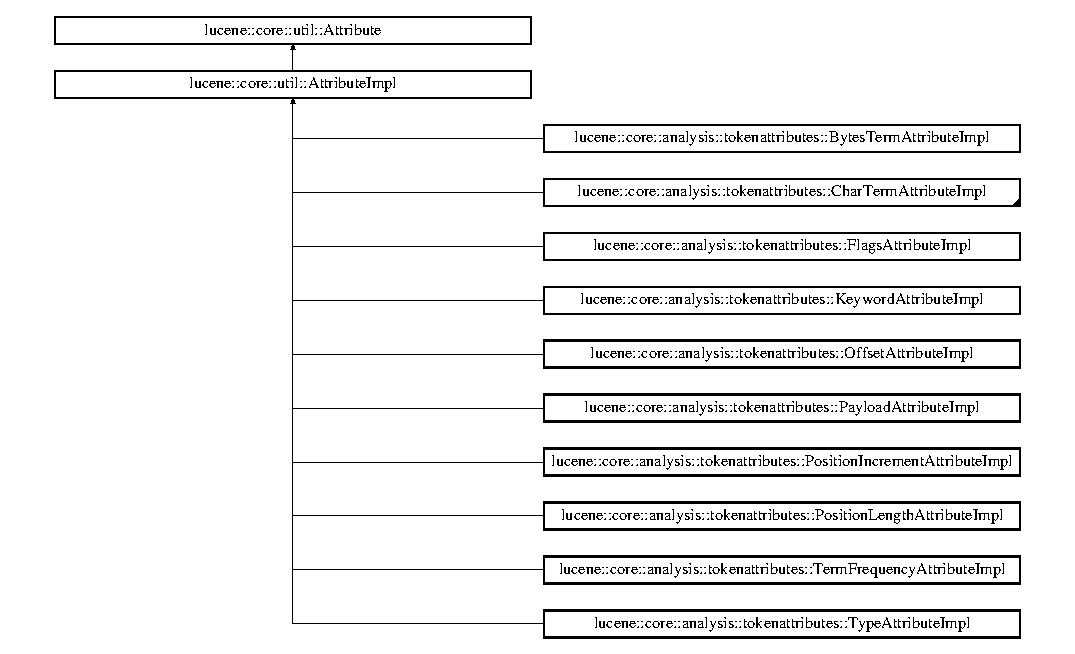
\includegraphics[height=8.337469cm]{classlucene_1_1core_1_1util_1_1AttributeImpl}
\end{center}
\end{figure}
\subsection*{Public Member Functions}
\begin{DoxyCompactItemize}
\item 
virtual \mbox{\hyperlink{classlucene_1_1core_1_1util_1_1AttributeImpl_aeaca9fe2fd952878945f12a519311ec4}{$\sim$\+Attribute\+Impl}} ()
\item 
virtual void \mbox{\hyperlink{classlucene_1_1core_1_1util_1_1AttributeImpl_a84d34275fb1ed67ac36fad7ff6388096}{Reflect\+With}} (\mbox{\hyperlink{namespacelucene_1_1core_1_1util_a7dbb701adaed055f73fb95eec83da10a}{Attribute\+Reflector}} \&reflector)=0
\item 
virtual void \mbox{\hyperlink{classlucene_1_1core_1_1util_1_1AttributeImpl_a04897a00a902f7a345dd44bbc4b482a8}{Clear}} ()=0
\item 
virtual void \mbox{\hyperlink{classlucene_1_1core_1_1util_1_1AttributeImpl_a9a662ddc9b72bc9711883a25b8379ea9}{End}} ()
\item 
virtual std\+::vector$<$ std\+::type\+\_\+index $>$ \mbox{\hyperlink{classlucene_1_1core_1_1util_1_1AttributeImpl_ac0631e6a7a11044883bc97447716d7cc}{Attributes}} ()=0
\item 
virtual void \mbox{\hyperlink{classlucene_1_1core_1_1util_1_1AttributeImpl_a010e8937832f53139c8fe42757476895}{Shallow\+Copy\+To}} (\mbox{\hyperlink{classlucene_1_1core_1_1util_1_1AttributeImpl}{Attribute\+Impl}} \&attr\+\_\+impl)=0
\item 
virtual \mbox{\hyperlink{classlucene_1_1core_1_1util_1_1AttributeImpl}{Attribute\+Impl}} $\ast$ \mbox{\hyperlink{classlucene_1_1core_1_1util_1_1AttributeImpl_a135318ad4c7c17b3d85e625e32fb42cd}{Clone}} ()=0
\item 
virtual \mbox{\hyperlink{classlucene_1_1core_1_1util_1_1AttributeImpl}{Attribute\+Impl}} \& \mbox{\hyperlink{classlucene_1_1core_1_1util_1_1AttributeImpl_ab032e399d03ce2f58c76881cf2b92325}{operator=}} (\mbox{\hyperlink{ZlibCrc32_8h_a2c212835823e3c54a8ab6d95c652660e}{const}} \mbox{\hyperlink{classlucene_1_1core_1_1util_1_1AttributeImpl}{Attribute\+Impl}} \&other)=0
\item 
std\+::string \mbox{\hyperlink{classlucene_1_1core_1_1util_1_1AttributeImpl_af3ad346d3dc7bbafa7957bcb48a9453e}{Reflect\+As\+String}} (\mbox{\hyperlink{ZlibCrc32_8h_a2c212835823e3c54a8ab6d95c652660e}{const}} bool prepend\+\_\+att\+\_\+class)
\end{DoxyCompactItemize}
\subsection*{Additional Inherited Members}


\subsection{Constructor \& Destructor Documentation}
\mbox{\Hypertarget{classlucene_1_1core_1_1util_1_1AttributeImpl_aeaca9fe2fd952878945f12a519311ec4}\label{classlucene_1_1core_1_1util_1_1AttributeImpl_aeaca9fe2fd952878945f12a519311ec4}} 
\index{lucene\+::core\+::util\+::\+Attribute\+Impl@{lucene\+::core\+::util\+::\+Attribute\+Impl}!````~Attribute\+Impl@{$\sim$\+Attribute\+Impl}}
\index{````~Attribute\+Impl@{$\sim$\+Attribute\+Impl}!lucene\+::core\+::util\+::\+Attribute\+Impl@{lucene\+::core\+::util\+::\+Attribute\+Impl}}
\subsubsection{\texorpdfstring{$\sim$\+Attribute\+Impl()}{~AttributeImpl()}}
{\footnotesize\ttfamily virtual lucene\+::core\+::util\+::\+Attribute\+Impl\+::$\sim$\+Attribute\+Impl (\begin{DoxyParamCaption}{ }\end{DoxyParamCaption})\hspace{0.3cm}{\ttfamily [inline]}, {\ttfamily [virtual]}}



\subsection{Member Function Documentation}
\mbox{\Hypertarget{classlucene_1_1core_1_1util_1_1AttributeImpl_ac0631e6a7a11044883bc97447716d7cc}\label{classlucene_1_1core_1_1util_1_1AttributeImpl_ac0631e6a7a11044883bc97447716d7cc}} 
\index{lucene\+::core\+::util\+::\+Attribute\+Impl@{lucene\+::core\+::util\+::\+Attribute\+Impl}!Attributes@{Attributes}}
\index{Attributes@{Attributes}!lucene\+::core\+::util\+::\+Attribute\+Impl@{lucene\+::core\+::util\+::\+Attribute\+Impl}}
\subsubsection{\texorpdfstring{Attributes()}{Attributes()}}
{\footnotesize\ttfamily virtual std\+::vector$<$std\+::type\+\_\+index$>$ lucene\+::core\+::util\+::\+Attribute\+Impl\+::\+Attributes (\begin{DoxyParamCaption}{ }\end{DoxyParamCaption})\hspace{0.3cm}{\ttfamily [pure virtual]}}



Implemented in \mbox{\hyperlink{classlucene_1_1core_1_1analysis_1_1tokenattributes_1_1TypeAttributeImpl_ae7ba4a6e94fb4f1d1c8111e613793d59}{lucene\+::core\+::analysis\+::tokenattributes\+::\+Type\+Attribute\+Impl}}, \mbox{\hyperlink{classlucene_1_1core_1_1analysis_1_1tokenattributes_1_1TermFrequencyAttributeImpl_a02e08b89bd1105326aff4d578c759886}{lucene\+::core\+::analysis\+::tokenattributes\+::\+Term\+Frequency\+Attribute\+Impl}}, \mbox{\hyperlink{classlucene_1_1core_1_1analysis_1_1tokenattributes_1_1PositionLengthAttributeImpl_abb480ef419ad8ee6c27a50e7eda1be29}{lucene\+::core\+::analysis\+::tokenattributes\+::\+Position\+Length\+Attribute\+Impl}}, \mbox{\hyperlink{classlucene_1_1core_1_1analysis_1_1tokenattributes_1_1PositionIncrementAttributeImpl_ab6028133ca375bdcb9774650828e7388}{lucene\+::core\+::analysis\+::tokenattributes\+::\+Position\+Increment\+Attribute\+Impl}}, \mbox{\hyperlink{classlucene_1_1core_1_1analysis_1_1tokenattributes_1_1PayloadAttributeImpl_a1f7dbb8afdd42ca827dc6e077445071b}{lucene\+::core\+::analysis\+::tokenattributes\+::\+Payload\+Attribute\+Impl}}, \mbox{\hyperlink{classlucene_1_1core_1_1analysis_1_1tokenattributes_1_1PackedTokenAttributeImpl_a450b5fd90cbf05268800b0f66eebb58f}{lucene\+::core\+::analysis\+::tokenattributes\+::\+Packed\+Token\+Attribute\+Impl}}, \mbox{\hyperlink{classlucene_1_1core_1_1analysis_1_1tokenattributes_1_1OffsetAttributeImpl_ac2f3c035417acfc9056a900903f1d271}{lucene\+::core\+::analysis\+::tokenattributes\+::\+Offset\+Attribute\+Impl}}, \mbox{\hyperlink{classlucene_1_1core_1_1analysis_1_1tokenattributes_1_1KeywordAttributeImpl_af338dde5485b5feb1b467fc07534f5cc}{lucene\+::core\+::analysis\+::tokenattributes\+::\+Keyword\+Attribute\+Impl}}, \mbox{\hyperlink{classlucene_1_1core_1_1analysis_1_1tokenattributes_1_1FlagsAttributeImpl_a3cdbd466551489b6f35ad51aa5ee2255}{lucene\+::core\+::analysis\+::tokenattributes\+::\+Flags\+Attribute\+Impl}}, \mbox{\hyperlink{classlucene_1_1core_1_1analysis_1_1tokenattributes_1_1CharTermAttributeImpl_a7d8986b373cd9c2dfb2de25dd12000fd}{lucene\+::core\+::analysis\+::tokenattributes\+::\+Char\+Term\+Attribute\+Impl}}, and \mbox{\hyperlink{classlucene_1_1core_1_1analysis_1_1tokenattributes_1_1BytesTermAttributeImpl_aff915b815335534889b45fa2ce773692}{lucene\+::core\+::analysis\+::tokenattributes\+::\+Bytes\+Term\+Attribute\+Impl}}.

\mbox{\Hypertarget{classlucene_1_1core_1_1util_1_1AttributeImpl_a04897a00a902f7a345dd44bbc4b482a8}\label{classlucene_1_1core_1_1util_1_1AttributeImpl_a04897a00a902f7a345dd44bbc4b482a8}} 
\index{lucene\+::core\+::util\+::\+Attribute\+Impl@{lucene\+::core\+::util\+::\+Attribute\+Impl}!Clear@{Clear}}
\index{Clear@{Clear}!lucene\+::core\+::util\+::\+Attribute\+Impl@{lucene\+::core\+::util\+::\+Attribute\+Impl}}
\subsubsection{\texorpdfstring{Clear()}{Clear()}}
{\footnotesize\ttfamily virtual void lucene\+::core\+::util\+::\+Attribute\+Impl\+::\+Clear (\begin{DoxyParamCaption}{ }\end{DoxyParamCaption})\hspace{0.3cm}{\ttfamily [pure virtual]}}



Implemented in \mbox{\hyperlink{classlucene_1_1core_1_1analysis_1_1tokenattributes_1_1TypeAttributeImpl_a373559195f408497ab81408bab95a2b1}{lucene\+::core\+::analysis\+::tokenattributes\+::\+Type\+Attribute\+Impl}}, \mbox{\hyperlink{classlucene_1_1core_1_1analysis_1_1tokenattributes_1_1TermFrequencyAttributeImpl_aaa575565a7b466b6bdcf4d8042f3f582}{lucene\+::core\+::analysis\+::tokenattributes\+::\+Term\+Frequency\+Attribute\+Impl}}, \mbox{\hyperlink{classlucene_1_1core_1_1analysis_1_1tokenattributes_1_1PositionLengthAttributeImpl_a0f4a9a4b9ab64ced895b8fa5b9983cbd}{lucene\+::core\+::analysis\+::tokenattributes\+::\+Position\+Length\+Attribute\+Impl}}, \mbox{\hyperlink{classlucene_1_1core_1_1analysis_1_1tokenattributes_1_1PositionIncrementAttributeImpl_a49cd1a34361a145c3b674f1f3d529641}{lucene\+::core\+::analysis\+::tokenattributes\+::\+Position\+Increment\+Attribute\+Impl}}, \mbox{\hyperlink{classlucene_1_1core_1_1analysis_1_1tokenattributes_1_1PayloadAttributeImpl_a264f13a218ec4caca8c724e3c34f64b6}{lucene\+::core\+::analysis\+::tokenattributes\+::\+Payload\+Attribute\+Impl}}, \mbox{\hyperlink{classlucene_1_1core_1_1analysis_1_1tokenattributes_1_1OffsetAttributeImpl_af19f560600cc53e48c592aa6d9c48a91}{lucene\+::core\+::analysis\+::tokenattributes\+::\+Offset\+Attribute\+Impl}}, \mbox{\hyperlink{classlucene_1_1core_1_1analysis_1_1tokenattributes_1_1KeywordAttributeImpl_a019bfed2dce94170444db84c7575f43c}{lucene\+::core\+::analysis\+::tokenattributes\+::\+Keyword\+Attribute\+Impl}}, \mbox{\hyperlink{classlucene_1_1core_1_1analysis_1_1tokenattributes_1_1FlagsAttributeImpl_a67ed39990f3f9eac90c91e880ad5cc31}{lucene\+::core\+::analysis\+::tokenattributes\+::\+Flags\+Attribute\+Impl}}, \mbox{\hyperlink{classlucene_1_1core_1_1analysis_1_1tokenattributes_1_1CharTermAttributeImpl_a4e0b1a5a06996822798414f3a41af6e6}{lucene\+::core\+::analysis\+::tokenattributes\+::\+Char\+Term\+Attribute\+Impl}}, and \mbox{\hyperlink{classlucene_1_1core_1_1analysis_1_1tokenattributes_1_1BytesTermAttributeImpl_a6fa48596a507c937bd874d46ef5ca963}{lucene\+::core\+::analysis\+::tokenattributes\+::\+Bytes\+Term\+Attribute\+Impl}}.

\mbox{\Hypertarget{classlucene_1_1core_1_1util_1_1AttributeImpl_a135318ad4c7c17b3d85e625e32fb42cd}\label{classlucene_1_1core_1_1util_1_1AttributeImpl_a135318ad4c7c17b3d85e625e32fb42cd}} 
\index{lucene\+::core\+::util\+::\+Attribute\+Impl@{lucene\+::core\+::util\+::\+Attribute\+Impl}!Clone@{Clone}}
\index{Clone@{Clone}!lucene\+::core\+::util\+::\+Attribute\+Impl@{lucene\+::core\+::util\+::\+Attribute\+Impl}}
\subsubsection{\texorpdfstring{Clone()}{Clone()}}
{\footnotesize\ttfamily virtual \mbox{\hyperlink{classlucene_1_1core_1_1util_1_1AttributeImpl}{Attribute\+Impl}}$\ast$ lucene\+::core\+::util\+::\+Attribute\+Impl\+::\+Clone (\begin{DoxyParamCaption}{ }\end{DoxyParamCaption})\hspace{0.3cm}{\ttfamily [pure virtual]}}



Implemented in \mbox{\hyperlink{classlucene_1_1core_1_1analysis_1_1tokenattributes_1_1TypeAttributeImpl_a3549b01075ae899b2e6dcfa7aa101eca}{lucene\+::core\+::analysis\+::tokenattributes\+::\+Type\+Attribute\+Impl}}, \mbox{\hyperlink{classlucene_1_1core_1_1analysis_1_1tokenattributes_1_1TermFrequencyAttributeImpl_a3d973d479d147e3feece05c9988bc7c6}{lucene\+::core\+::analysis\+::tokenattributes\+::\+Term\+Frequency\+Attribute\+Impl}}, \mbox{\hyperlink{classlucene_1_1core_1_1analysis_1_1tokenattributes_1_1PositionLengthAttributeImpl_a8880c22ea7f0cc06c2f7ed98900286aa}{lucene\+::core\+::analysis\+::tokenattributes\+::\+Position\+Length\+Attribute\+Impl}}, \mbox{\hyperlink{classlucene_1_1core_1_1analysis_1_1tokenattributes_1_1PositionIncrementAttributeImpl_a68907cad12693754f1286678a7c78c21}{lucene\+::core\+::analysis\+::tokenattributes\+::\+Position\+Increment\+Attribute\+Impl}}, \mbox{\hyperlink{classlucene_1_1core_1_1analysis_1_1tokenattributes_1_1PayloadAttributeImpl_a5ec30ffd50c79e22ba0166b0e47629b3}{lucene\+::core\+::analysis\+::tokenattributes\+::\+Payload\+Attribute\+Impl}}, \mbox{\hyperlink{classlucene_1_1core_1_1analysis_1_1tokenattributes_1_1PackedTokenAttributeImpl_ab96495b9ba0271afe2597425f925ee91}{lucene\+::core\+::analysis\+::tokenattributes\+::\+Packed\+Token\+Attribute\+Impl}}, \mbox{\hyperlink{classlucene_1_1core_1_1analysis_1_1tokenattributes_1_1OffsetAttributeImpl_a4cae4e770c4ce5184ae4530edde06bae}{lucene\+::core\+::analysis\+::tokenattributes\+::\+Offset\+Attribute\+Impl}}, \mbox{\hyperlink{classlucene_1_1core_1_1analysis_1_1tokenattributes_1_1KeywordAttributeImpl_a59d16bdfa3c456ebcd8b3ae90279cd7b}{lucene\+::core\+::analysis\+::tokenattributes\+::\+Keyword\+Attribute\+Impl}}, \mbox{\hyperlink{classlucene_1_1core_1_1analysis_1_1tokenattributes_1_1FlagsAttributeImpl_aa920978da58dffbf7eb16bfa5e5f84c4}{lucene\+::core\+::analysis\+::tokenattributes\+::\+Flags\+Attribute\+Impl}}, \mbox{\hyperlink{classlucene_1_1core_1_1analysis_1_1tokenattributes_1_1CharTermAttributeImpl_a518bf3f405ddf676ee58fccb02ae3c23}{lucene\+::core\+::analysis\+::tokenattributes\+::\+Char\+Term\+Attribute\+Impl}}, and \mbox{\hyperlink{classlucene_1_1core_1_1analysis_1_1tokenattributes_1_1BytesTermAttributeImpl_a149760a0122009e6b699862553d43b41}{lucene\+::core\+::analysis\+::tokenattributes\+::\+Bytes\+Term\+Attribute\+Impl}}.

\mbox{\Hypertarget{classlucene_1_1core_1_1util_1_1AttributeImpl_a9a662ddc9b72bc9711883a25b8379ea9}\label{classlucene_1_1core_1_1util_1_1AttributeImpl_a9a662ddc9b72bc9711883a25b8379ea9}} 
\index{lucene\+::core\+::util\+::\+Attribute\+Impl@{lucene\+::core\+::util\+::\+Attribute\+Impl}!End@{End}}
\index{End@{End}!lucene\+::core\+::util\+::\+Attribute\+Impl@{lucene\+::core\+::util\+::\+Attribute\+Impl}}
\subsubsection{\texorpdfstring{End()}{End()}}
{\footnotesize\ttfamily void Attribute\+Impl\+::\+End (\begin{DoxyParamCaption}{ }\end{DoxyParamCaption})\hspace{0.3cm}{\ttfamily [virtual]}}

\mbox{\hyperlink{classlucene_1_1core_1_1util_1_1AttributeImpl}{Attribute\+Impl}} 

Reimplemented in \mbox{\hyperlink{classlucene_1_1core_1_1analysis_1_1tokenattributes_1_1PositionIncrementAttributeImpl_adb934ddcbf6f584c50a72c0980b88761}{lucene\+::core\+::analysis\+::tokenattributes\+::\+Position\+Increment\+Attribute\+Impl}}.

\mbox{\Hypertarget{classlucene_1_1core_1_1util_1_1AttributeImpl_ab032e399d03ce2f58c76881cf2b92325}\label{classlucene_1_1core_1_1util_1_1AttributeImpl_ab032e399d03ce2f58c76881cf2b92325}} 
\index{lucene\+::core\+::util\+::\+Attribute\+Impl@{lucene\+::core\+::util\+::\+Attribute\+Impl}!operator=@{operator=}}
\index{operator=@{operator=}!lucene\+::core\+::util\+::\+Attribute\+Impl@{lucene\+::core\+::util\+::\+Attribute\+Impl}}
\subsubsection{\texorpdfstring{operator=()}{operator=()}}
{\footnotesize\ttfamily virtual \mbox{\hyperlink{classlucene_1_1core_1_1util_1_1AttributeImpl}{Attribute\+Impl}}\& lucene\+::core\+::util\+::\+Attribute\+Impl\+::operator= (\begin{DoxyParamCaption}\item[{\mbox{\hyperlink{ZlibCrc32_8h_a2c212835823e3c54a8ab6d95c652660e}{const}} \mbox{\hyperlink{classlucene_1_1core_1_1util_1_1AttributeImpl}{Attribute\+Impl}} \&}]{other }\end{DoxyParamCaption})\hspace{0.3cm}{\ttfamily [pure virtual]}}



Implemented in \mbox{\hyperlink{classlucene_1_1core_1_1analysis_1_1tokenattributes_1_1TypeAttributeImpl_a873153f88f6ec5485c4a0bed1374bb9b}{lucene\+::core\+::analysis\+::tokenattributes\+::\+Type\+Attribute\+Impl}}, \mbox{\hyperlink{classlucene_1_1core_1_1analysis_1_1tokenattributes_1_1TermFrequencyAttributeImpl_a855437532aa60208023e367fe09926fd}{lucene\+::core\+::analysis\+::tokenattributes\+::\+Term\+Frequency\+Attribute\+Impl}}, \mbox{\hyperlink{classlucene_1_1core_1_1analysis_1_1tokenattributes_1_1PositionLengthAttributeImpl_a40bda49e6da62bc1c16e8ef11525d840}{lucene\+::core\+::analysis\+::tokenattributes\+::\+Position\+Length\+Attribute\+Impl}}, \mbox{\hyperlink{classlucene_1_1core_1_1analysis_1_1tokenattributes_1_1PositionIncrementAttributeImpl_a8fccb463e29cc9cb90e7689cc7161488}{lucene\+::core\+::analysis\+::tokenattributes\+::\+Position\+Increment\+Attribute\+Impl}}, \mbox{\hyperlink{classlucene_1_1core_1_1analysis_1_1tokenattributes_1_1PayloadAttributeImpl_a82dd546c2275107d47d6a152cd43d04e}{lucene\+::core\+::analysis\+::tokenattributes\+::\+Payload\+Attribute\+Impl}}, \mbox{\hyperlink{classlucene_1_1core_1_1analysis_1_1tokenattributes_1_1PackedTokenAttributeImpl_a9519720f5eb790ef3e796cefbcbecc96}{lucene\+::core\+::analysis\+::tokenattributes\+::\+Packed\+Token\+Attribute\+Impl}}, \mbox{\hyperlink{classlucene_1_1core_1_1analysis_1_1tokenattributes_1_1OffsetAttributeImpl_ad5aee8c4731cfda2c9a1c7b7dbe4dc30}{lucene\+::core\+::analysis\+::tokenattributes\+::\+Offset\+Attribute\+Impl}}, \mbox{\hyperlink{classlucene_1_1core_1_1analysis_1_1tokenattributes_1_1KeywordAttributeImpl_a30228ce41cc678c1cb85c2fb1179f447}{lucene\+::core\+::analysis\+::tokenattributes\+::\+Keyword\+Attribute\+Impl}}, \mbox{\hyperlink{classlucene_1_1core_1_1analysis_1_1tokenattributes_1_1FlagsAttributeImpl_a41dfb20fafc327e7832e639695b453fa}{lucene\+::core\+::analysis\+::tokenattributes\+::\+Flags\+Attribute\+Impl}}, \mbox{\hyperlink{classlucene_1_1core_1_1analysis_1_1tokenattributes_1_1CharTermAttributeImpl_ac49b714c3f8e438ddaa27dc1a2421144}{lucene\+::core\+::analysis\+::tokenattributes\+::\+Char\+Term\+Attribute\+Impl}}, and \mbox{\hyperlink{classlucene_1_1core_1_1analysis_1_1tokenattributes_1_1BytesTermAttributeImpl_acfaef15f10ddfec3e2494c6d2176ac73}{lucene\+::core\+::analysis\+::tokenattributes\+::\+Bytes\+Term\+Attribute\+Impl}}.

\mbox{\Hypertarget{classlucene_1_1core_1_1util_1_1AttributeImpl_af3ad346d3dc7bbafa7957bcb48a9453e}\label{classlucene_1_1core_1_1util_1_1AttributeImpl_af3ad346d3dc7bbafa7957bcb48a9453e}} 
\index{lucene\+::core\+::util\+::\+Attribute\+Impl@{lucene\+::core\+::util\+::\+Attribute\+Impl}!Reflect\+As\+String@{Reflect\+As\+String}}
\index{Reflect\+As\+String@{Reflect\+As\+String}!lucene\+::core\+::util\+::\+Attribute\+Impl@{lucene\+::core\+::util\+::\+Attribute\+Impl}}
\subsubsection{\texorpdfstring{Reflect\+As\+String()}{ReflectAsString()}}
{\footnotesize\ttfamily std\+::string Attribute\+Impl\+::\+Reflect\+As\+String (\begin{DoxyParamCaption}\item[{\mbox{\hyperlink{ZlibCrc32_8h_a2c212835823e3c54a8ab6d95c652660e}{const}} bool}]{prepend\+\_\+att\+\_\+class }\end{DoxyParamCaption})}

\mbox{\Hypertarget{classlucene_1_1core_1_1util_1_1AttributeImpl_a84d34275fb1ed67ac36fad7ff6388096}\label{classlucene_1_1core_1_1util_1_1AttributeImpl_a84d34275fb1ed67ac36fad7ff6388096}} 
\index{lucene\+::core\+::util\+::\+Attribute\+Impl@{lucene\+::core\+::util\+::\+Attribute\+Impl}!Reflect\+With@{Reflect\+With}}
\index{Reflect\+With@{Reflect\+With}!lucene\+::core\+::util\+::\+Attribute\+Impl@{lucene\+::core\+::util\+::\+Attribute\+Impl}}
\subsubsection{\texorpdfstring{Reflect\+With()}{ReflectWith()}}
{\footnotesize\ttfamily virtual void lucene\+::core\+::util\+::\+Attribute\+Impl\+::\+Reflect\+With (\begin{DoxyParamCaption}\item[{\mbox{\hyperlink{namespacelucene_1_1core_1_1util_a7dbb701adaed055f73fb95eec83da10a}{Attribute\+Reflector}} \&}]{reflector }\end{DoxyParamCaption})\hspace{0.3cm}{\ttfamily [pure virtual]}}



Implemented in \mbox{\hyperlink{classlucene_1_1core_1_1analysis_1_1tokenattributes_1_1TypeAttributeImpl_a7194a1e268786f0a45e77b1204246727}{lucene\+::core\+::analysis\+::tokenattributes\+::\+Type\+Attribute\+Impl}}, \mbox{\hyperlink{classlucene_1_1core_1_1analysis_1_1tokenattributes_1_1TermFrequencyAttributeImpl_aef08e2be7b9a57329ed5df12fcb2a9d9}{lucene\+::core\+::analysis\+::tokenattributes\+::\+Term\+Frequency\+Attribute\+Impl}}, \mbox{\hyperlink{classlucene_1_1core_1_1analysis_1_1tokenattributes_1_1PositionLengthAttributeImpl_aec63a5cf6bdf55b0f4c95d5b17109e5f}{lucene\+::core\+::analysis\+::tokenattributes\+::\+Position\+Length\+Attribute\+Impl}}, \mbox{\hyperlink{classlucene_1_1core_1_1analysis_1_1tokenattributes_1_1PositionIncrementAttributeImpl_a2ede3f15304f9760ad60009335123ece}{lucene\+::core\+::analysis\+::tokenattributes\+::\+Position\+Increment\+Attribute\+Impl}}, \mbox{\hyperlink{classlucene_1_1core_1_1analysis_1_1tokenattributes_1_1PayloadAttributeImpl_ab012363b8b4ce7e15c9c91ba6ec0c325}{lucene\+::core\+::analysis\+::tokenattributes\+::\+Payload\+Attribute\+Impl}}, \mbox{\hyperlink{classlucene_1_1core_1_1analysis_1_1tokenattributes_1_1OffsetAttributeImpl_ad7eb3a266863f7e14fbe1caa315c7151}{lucene\+::core\+::analysis\+::tokenattributes\+::\+Offset\+Attribute\+Impl}}, \mbox{\hyperlink{classlucene_1_1core_1_1analysis_1_1tokenattributes_1_1KeywordAttributeImpl_a610aab1880b02caf13fb7f1723c24c94}{lucene\+::core\+::analysis\+::tokenattributes\+::\+Keyword\+Attribute\+Impl}}, \mbox{\hyperlink{classlucene_1_1core_1_1analysis_1_1tokenattributes_1_1FlagsAttributeImpl_aa479cdc4474246af90f7d54ca64d3a48}{lucene\+::core\+::analysis\+::tokenattributes\+::\+Flags\+Attribute\+Impl}}, \mbox{\hyperlink{classlucene_1_1core_1_1analysis_1_1tokenattributes_1_1CharTermAttributeImpl_ae434068c40b8eab62af50e0e33a71bf4}{lucene\+::core\+::analysis\+::tokenattributes\+::\+Char\+Term\+Attribute\+Impl}}, and \mbox{\hyperlink{classlucene_1_1core_1_1analysis_1_1tokenattributes_1_1BytesTermAttributeImpl_a6a1789244604f807529de975d4c10171}{lucene\+::core\+::analysis\+::tokenattributes\+::\+Bytes\+Term\+Attribute\+Impl}}.

\mbox{\Hypertarget{classlucene_1_1core_1_1util_1_1AttributeImpl_a010e8937832f53139c8fe42757476895}\label{classlucene_1_1core_1_1util_1_1AttributeImpl_a010e8937832f53139c8fe42757476895}} 
\index{lucene\+::core\+::util\+::\+Attribute\+Impl@{lucene\+::core\+::util\+::\+Attribute\+Impl}!Shallow\+Copy\+To@{Shallow\+Copy\+To}}
\index{Shallow\+Copy\+To@{Shallow\+Copy\+To}!lucene\+::core\+::util\+::\+Attribute\+Impl@{lucene\+::core\+::util\+::\+Attribute\+Impl}}
\subsubsection{\texorpdfstring{Shallow\+Copy\+To()}{ShallowCopyTo()}}
{\footnotesize\ttfamily virtual void lucene\+::core\+::util\+::\+Attribute\+Impl\+::\+Shallow\+Copy\+To (\begin{DoxyParamCaption}\item[{\mbox{\hyperlink{classlucene_1_1core_1_1util_1_1AttributeImpl}{Attribute\+Impl}} \&}]{attr\+\_\+impl }\end{DoxyParamCaption})\hspace{0.3cm}{\ttfamily [pure virtual]}}



Implemented in \mbox{\hyperlink{classlucene_1_1core_1_1analysis_1_1tokenattributes_1_1TypeAttributeImpl_a2eefa7e33a6e060c5493711cd60c9d2e}{lucene\+::core\+::analysis\+::tokenattributes\+::\+Type\+Attribute\+Impl}}, \mbox{\hyperlink{classlucene_1_1core_1_1analysis_1_1tokenattributes_1_1TermFrequencyAttributeImpl_a82c1cb2877fab77b907b4b03795d0fdf}{lucene\+::core\+::analysis\+::tokenattributes\+::\+Term\+Frequency\+Attribute\+Impl}}, \mbox{\hyperlink{classlucene_1_1core_1_1analysis_1_1tokenattributes_1_1PositionLengthAttributeImpl_a657ca7b71ea00d5ba609453d0333cafa}{lucene\+::core\+::analysis\+::tokenattributes\+::\+Position\+Length\+Attribute\+Impl}}, \mbox{\hyperlink{classlucene_1_1core_1_1analysis_1_1tokenattributes_1_1PositionIncrementAttributeImpl_a887e391d3db93f6a8e76b6b464d60547}{lucene\+::core\+::analysis\+::tokenattributes\+::\+Position\+Increment\+Attribute\+Impl}}, \mbox{\hyperlink{classlucene_1_1core_1_1analysis_1_1tokenattributes_1_1PayloadAttributeImpl_ae1104df0b599fd494620e2bce9d39b6c}{lucene\+::core\+::analysis\+::tokenattributes\+::\+Payload\+Attribute\+Impl}}, \mbox{\hyperlink{classlucene_1_1core_1_1analysis_1_1tokenattributes_1_1PackedTokenAttributeImpl_ab89c820321f0f5b84c7a392bb8de32f3}{lucene\+::core\+::analysis\+::tokenattributes\+::\+Packed\+Token\+Attribute\+Impl}}, \mbox{\hyperlink{classlucene_1_1core_1_1analysis_1_1tokenattributes_1_1OffsetAttributeImpl_a426d0cd75306c4ef7cec3c28e34c0029}{lucene\+::core\+::analysis\+::tokenattributes\+::\+Offset\+Attribute\+Impl}}, \mbox{\hyperlink{classlucene_1_1core_1_1analysis_1_1tokenattributes_1_1KeywordAttributeImpl_a83f442881b35bc26a6edb2e04beeb58a}{lucene\+::core\+::analysis\+::tokenattributes\+::\+Keyword\+Attribute\+Impl}}, \mbox{\hyperlink{classlucene_1_1core_1_1analysis_1_1tokenattributes_1_1FlagsAttributeImpl_a9c6a676eb175556a2eea6afaae666f8d}{lucene\+::core\+::analysis\+::tokenattributes\+::\+Flags\+Attribute\+Impl}}, \mbox{\hyperlink{classlucene_1_1core_1_1analysis_1_1tokenattributes_1_1CharTermAttributeImpl_ae37cc1fbce5614f5e60800d3f9f96d33}{lucene\+::core\+::analysis\+::tokenattributes\+::\+Char\+Term\+Attribute\+Impl}}, and \mbox{\hyperlink{classlucene_1_1core_1_1analysis_1_1tokenattributes_1_1BytesTermAttributeImpl_aafc25a873ed04661a26d6a7b5f6d2b0d}{lucene\+::core\+::analysis\+::tokenattributes\+::\+Bytes\+Term\+Attribute\+Impl}}.



The documentation for this class was generated from the following files\+:\begin{DoxyCompactItemize}
\item 
Util/\mbox{\hyperlink{Util_2Attribute_8h}{Attribute.\+h}}\item 
Util/\mbox{\hyperlink{Util_2Attribute_8cpp}{Attribute.\+cpp}}\end{DoxyCompactItemize}

\hypertarget{classlucene_1_1core_1_1util_1_1AttributeSource}{}\section{lucene\+:\+:core\+:\+:util\+:\+:Attribute\+Source Class Reference}
\label{classlucene_1_1core_1_1util_1_1AttributeSource}\index{lucene\+::core\+::util\+::\+Attribute\+Source@{lucene\+::core\+::util\+::\+Attribute\+Source}}


{\ttfamily \#include $<$Attribute.\+h$>$}

Inheritance diagram for lucene\+:\+:core\+:\+:util\+:\+:Attribute\+Source\+:\begin{figure}[H]
\begin{center}
\leavevmode
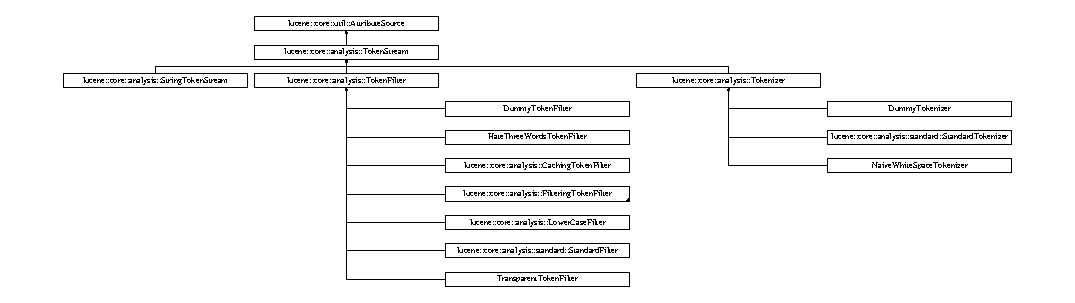
\includegraphics[height=3.020496cm]{classlucene_1_1core_1_1util_1_1AttributeSource}
\end{center}
\end{figure}
\subsection*{Classes}
\begin{DoxyCompactItemize}
\item 
class \mbox{\hyperlink{classlucene_1_1core_1_1util_1_1AttributeSource_1_1State}{State}}
\item 
class \mbox{\hyperlink{classlucene_1_1core_1_1util_1_1AttributeSource_1_1StateHolder}{State\+Holder}}
\end{DoxyCompactItemize}
\subsection*{Public Member Functions}
\begin{DoxyCompactItemize}
\item 
\mbox{\hyperlink{classlucene_1_1core_1_1util_1_1AttributeSource_aef30fddd7e976cf96938778e73ebba1f}{Attribute\+Source}} ()
\item 
\mbox{\hyperlink{classlucene_1_1core_1_1util_1_1AttributeSource_a46285603ecad877610be674c124fd632}{Attribute\+Source}} (\mbox{\hyperlink{ZlibCrc32_8h_a2c212835823e3c54a8ab6d95c652660e}{const}} \mbox{\hyperlink{classlucene_1_1core_1_1util_1_1AttributeSource}{Attribute\+Source}} \&other)
\item 
\mbox{\hyperlink{classlucene_1_1core_1_1util_1_1AttributeSource_a3111b8c073c694240c1797420c7031a3}{Attribute\+Source}} (\mbox{\hyperlink{classlucene_1_1core_1_1util_1_1AttributeFactory}{Attribute\+Factory}} \&\mbox{\hyperlink{classlucene_1_1core_1_1util_1_1AttributeSource_a1376420a752f337a0fdb582bdf160eba}{factory}})
\item 
\mbox{\hyperlink{classlucene_1_1core_1_1util_1_1AttributeFactory}{Attribute\+Factory}} \& \mbox{\hyperlink{classlucene_1_1core_1_1util_1_1AttributeSource_ab361967a0235e8d9f1afab451d5d2e99}{Get\+Attribute\+Factory}} () \mbox{\hyperlink{ZlibCrc32_8h_a2c212835823e3c54a8ab6d95c652660e}{const}}
\item 
void \mbox{\hyperlink{classlucene_1_1core_1_1util_1_1AttributeSource_a5aeee12f7ccd43874a1bc2447f3e54ac}{Add\+Attribute\+Impl}} (\mbox{\hyperlink{classlucene_1_1core_1_1util_1_1AttributeImpl}{Attribute\+Impl}} $\ast$attr\+\_\+impl)
\item 
{\footnotesize template$<$typename A\+T\+TR $>$ }\\std\+::shared\+\_\+ptr$<$ A\+T\+TR $>$ \mbox{\hyperlink{classlucene_1_1core_1_1util_1_1AttributeSource_af07d54141811dd0711441530dffc5e8f}{Add\+Attribute}} ()
\item 
bool \mbox{\hyperlink{classlucene_1_1core_1_1util_1_1AttributeSource_a885ff0d539fc9d2763412c18f5c19097}{Has\+Attributes}} ()
\item 
{\footnotesize template$<$typename A\+T\+TR $>$ }\\bool \mbox{\hyperlink{classlucene_1_1core_1_1util_1_1AttributeSource_a214d5ca7edcf7bed74db8d73c73f9802}{Has\+Attribute}} ()
\item 
void \mbox{\hyperlink{classlucene_1_1core_1_1util_1_1AttributeSource_a7c2b117da3dac9f29017a5bb5562d6de}{Clear\+Attributes}} ()
\item 
void \mbox{\hyperlink{classlucene_1_1core_1_1util_1_1AttributeSource_a52fad6b087a947622e3f4485357f78b2}{End\+Attributes}} ()
\item 
void \mbox{\hyperlink{classlucene_1_1core_1_1util_1_1AttributeSource_af3f3c9582d3ac28feaa7a455fbb24b80}{Remove\+All\+Attributes}} ()
\item 
\mbox{\hyperlink{classlucene_1_1core_1_1util_1_1AttributeSource_1_1State}{State}} $\ast$ \mbox{\hyperlink{classlucene_1_1core_1_1util_1_1AttributeSource_adb86fb2ab1b48c7643cf7f0f641cb8ce}{Capture\+State}} ()
\item 
void \mbox{\hyperlink{classlucene_1_1core_1_1util_1_1AttributeSource_a1b58ab9c3125d5c6c05ed47e021d455c}{Restore\+State}} (\mbox{\hyperlink{classlucene_1_1core_1_1util_1_1AttributeSource_1_1State}{State}} $\ast$state)
\item 
std\+::string \mbox{\hyperlink{classlucene_1_1core_1_1util_1_1AttributeSource_a666406f74bc169662d4f54020ac7ddab}{Reflect\+As\+String}} (\mbox{\hyperlink{ZlibCrc32_8h_a2c212835823e3c54a8ab6d95c652660e}{const}} bool prepend\+\_\+att)
\item 
void \mbox{\hyperlink{classlucene_1_1core_1_1util_1_1AttributeSource_a2c1c0eeec6866335e6b44e1fa83a97f9}{Reflect\+With}} (\mbox{\hyperlink{namespacelucene_1_1core_1_1util_a7dbb701adaed055f73fb95eec83da10a}{Attribute\+Reflector}} \&reflector)
\item 
\mbox{\hyperlink{classlucene_1_1core_1_1util_1_1AttributeSource}{Attribute\+Source}} \& \mbox{\hyperlink{classlucene_1_1core_1_1util_1_1AttributeSource_acc3081e1437b1c96ddc7671b5088c460}{operator=}} (\mbox{\hyperlink{ZlibCrc32_8h_a2c212835823e3c54a8ab6d95c652660e}{const}} \mbox{\hyperlink{classlucene_1_1core_1_1util_1_1AttributeSource}{Attribute\+Source}} \&other)
\item 
void \mbox{\hyperlink{classlucene_1_1core_1_1util_1_1AttributeSource_a9fd48c63c575c5c69818d3697c17a9a3}{Shallow\+Copy\+To}} (\mbox{\hyperlink{classlucene_1_1core_1_1util_1_1AttributeSource}{Attribute\+Source}} \&other) \mbox{\hyperlink{ZlibCrc32_8h_a2c212835823e3c54a8ab6d95c652660e}{const}}
\end{DoxyCompactItemize}
\subsection*{Private Member Functions}
\begin{DoxyCompactItemize}
\item 
\mbox{\hyperlink{classlucene_1_1core_1_1util_1_1AttributeSource_1_1State}{State}} $\ast$ \mbox{\hyperlink{classlucene_1_1core_1_1util_1_1AttributeSource_a7a8f566041a7140d8ff8d6bea8e45b0f}{Get\+Current\+State}} ()
\end{DoxyCompactItemize}
\subsection*{Private Attributes}
\begin{DoxyCompactItemize}
\item 
\mbox{\hyperlink{classlucene_1_1core_1_1util_1_1AttributeSource_1_1StateHolder}{State\+Holder}} \mbox{\hyperlink{classlucene_1_1core_1_1util_1_1AttributeSource_a62ac9cefce936c5e903da6f3d9c9f31c}{state\+\_\+holder}}
\item 
std\+::unordered\+\_\+map$<$ std\+::type\+\_\+index, std\+::shared\+\_\+ptr$<$ \mbox{\hyperlink{classlucene_1_1core_1_1util_1_1AttributeImpl}{Attribute\+Impl}} $>$ $>$ \mbox{\hyperlink{classlucene_1_1core_1_1util_1_1AttributeSource_aa1994ef1eaa78a84c4371a0a286b5c69}{attributes}}
\item 
std\+::unordered\+\_\+map$<$ std\+::type\+\_\+index, std\+::shared\+\_\+ptr$<$ \mbox{\hyperlink{classlucene_1_1core_1_1util_1_1AttributeImpl}{Attribute\+Impl}} $>$ $>$ \mbox{\hyperlink{classlucene_1_1core_1_1util_1_1AttributeSource_afd81d39723b99832ecafe9aa538181e3}{attribute\+\_\+impls}}
\item 
\mbox{\hyperlink{classlucene_1_1core_1_1util_1_1AttributeFactory}{Attribute\+Factory}} \& \mbox{\hyperlink{classlucene_1_1core_1_1util_1_1AttributeSource_a1376420a752f337a0fdb582bdf160eba}{factory}}
\end{DoxyCompactItemize}


\subsection{Constructor \& Destructor Documentation}
\mbox{\Hypertarget{classlucene_1_1core_1_1util_1_1AttributeSource_aef30fddd7e976cf96938778e73ebba1f}\label{classlucene_1_1core_1_1util_1_1AttributeSource_aef30fddd7e976cf96938778e73ebba1f}} 
\index{lucene\+::core\+::util\+::\+Attribute\+Source@{lucene\+::core\+::util\+::\+Attribute\+Source}!Attribute\+Source@{Attribute\+Source}}
\index{Attribute\+Source@{Attribute\+Source}!lucene\+::core\+::util\+::\+Attribute\+Source@{lucene\+::core\+::util\+::\+Attribute\+Source}}
\subsubsection{\texorpdfstring{Attribute\+Source()}{AttributeSource()}\hspace{0.1cm}{\footnotesize\ttfamily [1/3]}}
{\footnotesize\ttfamily Attribute\+Source\+::\+Attribute\+Source (\begin{DoxyParamCaption}{ }\end{DoxyParamCaption})}

\mbox{\hyperlink{classlucene_1_1core_1_1util_1_1AttributeSource}{Attribute\+Source}} \mbox{\Hypertarget{classlucene_1_1core_1_1util_1_1AttributeSource_a46285603ecad877610be674c124fd632}\label{classlucene_1_1core_1_1util_1_1AttributeSource_a46285603ecad877610be674c124fd632}} 
\index{lucene\+::core\+::util\+::\+Attribute\+Source@{lucene\+::core\+::util\+::\+Attribute\+Source}!Attribute\+Source@{Attribute\+Source}}
\index{Attribute\+Source@{Attribute\+Source}!lucene\+::core\+::util\+::\+Attribute\+Source@{lucene\+::core\+::util\+::\+Attribute\+Source}}
\subsubsection{\texorpdfstring{Attribute\+Source()}{AttributeSource()}\hspace{0.1cm}{\footnotesize\ttfamily [2/3]}}
{\footnotesize\ttfamily Attribute\+Source\+::\+Attribute\+Source (\begin{DoxyParamCaption}\item[{\mbox{\hyperlink{ZlibCrc32_8h_a2c212835823e3c54a8ab6d95c652660e}{const}} \mbox{\hyperlink{classlucene_1_1core_1_1util_1_1AttributeSource}{Attribute\+Source}} \&}]{other }\end{DoxyParamCaption})}

\mbox{\Hypertarget{classlucene_1_1core_1_1util_1_1AttributeSource_a3111b8c073c694240c1797420c7031a3}\label{classlucene_1_1core_1_1util_1_1AttributeSource_a3111b8c073c694240c1797420c7031a3}} 
\index{lucene\+::core\+::util\+::\+Attribute\+Source@{lucene\+::core\+::util\+::\+Attribute\+Source}!Attribute\+Source@{Attribute\+Source}}
\index{Attribute\+Source@{Attribute\+Source}!lucene\+::core\+::util\+::\+Attribute\+Source@{lucene\+::core\+::util\+::\+Attribute\+Source}}
\subsubsection{\texorpdfstring{Attribute\+Source()}{AttributeSource()}\hspace{0.1cm}{\footnotesize\ttfamily [3/3]}}
{\footnotesize\ttfamily Attribute\+Source\+::\+Attribute\+Source (\begin{DoxyParamCaption}\item[{\mbox{\hyperlink{classlucene_1_1core_1_1util_1_1AttributeFactory}{Attribute\+Factory}} \&}]{factory }\end{DoxyParamCaption})\hspace{0.3cm}{\ttfamily [explicit]}}

\mbox{\hyperlink{classlucene_1_1core_1_1util_1_1AttributeSource}{Attribute\+Source}} consturctor. \mbox{\hyperlink{classlucene_1_1core_1_1util_1_1AttributeSource}{Attribute\+Source}} shares a given factory. So factory\textquotesingle{}s life cycle is not managed by this instance. 

\subsection{Member Function Documentation}
\mbox{\Hypertarget{classlucene_1_1core_1_1util_1_1AttributeSource_af07d54141811dd0711441530dffc5e8f}\label{classlucene_1_1core_1_1util_1_1AttributeSource_af07d54141811dd0711441530dffc5e8f}} 
\index{lucene\+::core\+::util\+::\+Attribute\+Source@{lucene\+::core\+::util\+::\+Attribute\+Source}!Add\+Attribute@{Add\+Attribute}}
\index{Add\+Attribute@{Add\+Attribute}!lucene\+::core\+::util\+::\+Attribute\+Source@{lucene\+::core\+::util\+::\+Attribute\+Source}}
\subsubsection{\texorpdfstring{Add\+Attribute()}{AddAttribute()}}
{\footnotesize\ttfamily template$<$typename A\+T\+TR $>$ \\
std\+::shared\+\_\+ptr$<$A\+T\+TR$>$ lucene\+::core\+::util\+::\+Attribute\+Source\+::\+Add\+Attribute (\begin{DoxyParamCaption}{ }\end{DoxyParamCaption})\hspace{0.3cm}{\ttfamily [inline]}}

\mbox{\Hypertarget{classlucene_1_1core_1_1util_1_1AttributeSource_a5aeee12f7ccd43874a1bc2447f3e54ac}\label{classlucene_1_1core_1_1util_1_1AttributeSource_a5aeee12f7ccd43874a1bc2447f3e54ac}} 
\index{lucene\+::core\+::util\+::\+Attribute\+Source@{lucene\+::core\+::util\+::\+Attribute\+Source}!Add\+Attribute\+Impl@{Add\+Attribute\+Impl}}
\index{Add\+Attribute\+Impl@{Add\+Attribute\+Impl}!lucene\+::core\+::util\+::\+Attribute\+Source@{lucene\+::core\+::util\+::\+Attribute\+Source}}
\subsubsection{\texorpdfstring{Add\+Attribute\+Impl()}{AddAttributeImpl()}}
{\footnotesize\ttfamily void Attribute\+Source\+::\+Add\+Attribute\+Impl (\begin{DoxyParamCaption}\item[{\mbox{\hyperlink{classlucene_1_1core_1_1util_1_1AttributeImpl}{Attribute\+Impl}} $\ast$}]{attr\+\_\+impl }\end{DoxyParamCaption})}

\mbox{\Hypertarget{classlucene_1_1core_1_1util_1_1AttributeSource_adb86fb2ab1b48c7643cf7f0f641cb8ce}\label{classlucene_1_1core_1_1util_1_1AttributeSource_adb86fb2ab1b48c7643cf7f0f641cb8ce}} 
\index{lucene\+::core\+::util\+::\+Attribute\+Source@{lucene\+::core\+::util\+::\+Attribute\+Source}!Capture\+State@{Capture\+State}}
\index{Capture\+State@{Capture\+State}!lucene\+::core\+::util\+::\+Attribute\+Source@{lucene\+::core\+::util\+::\+Attribute\+Source}}
\subsubsection{\texorpdfstring{Capture\+State()}{CaptureState()}}
{\footnotesize\ttfamily \mbox{\hyperlink{classlucene_1_1core_1_1util_1_1AttributeSource_1_1State}{Attribute\+Source\+::\+State}} $\ast$ Attribute\+Source\+::\+Capture\+State (\begin{DoxyParamCaption}{ }\end{DoxyParamCaption})}

\mbox{\Hypertarget{classlucene_1_1core_1_1util_1_1AttributeSource_a7c2b117da3dac9f29017a5bb5562d6de}\label{classlucene_1_1core_1_1util_1_1AttributeSource_a7c2b117da3dac9f29017a5bb5562d6de}} 
\index{lucene\+::core\+::util\+::\+Attribute\+Source@{lucene\+::core\+::util\+::\+Attribute\+Source}!Clear\+Attributes@{Clear\+Attributes}}
\index{Clear\+Attributes@{Clear\+Attributes}!lucene\+::core\+::util\+::\+Attribute\+Source@{lucene\+::core\+::util\+::\+Attribute\+Source}}
\subsubsection{\texorpdfstring{Clear\+Attributes()}{ClearAttributes()}}
{\footnotesize\ttfamily void Attribute\+Source\+::\+Clear\+Attributes (\begin{DoxyParamCaption}{ }\end{DoxyParamCaption})}

\mbox{\Hypertarget{classlucene_1_1core_1_1util_1_1AttributeSource_a52fad6b087a947622e3f4485357f78b2}\label{classlucene_1_1core_1_1util_1_1AttributeSource_a52fad6b087a947622e3f4485357f78b2}} 
\index{lucene\+::core\+::util\+::\+Attribute\+Source@{lucene\+::core\+::util\+::\+Attribute\+Source}!End\+Attributes@{End\+Attributes}}
\index{End\+Attributes@{End\+Attributes}!lucene\+::core\+::util\+::\+Attribute\+Source@{lucene\+::core\+::util\+::\+Attribute\+Source}}
\subsubsection{\texorpdfstring{End\+Attributes()}{EndAttributes()}}
{\footnotesize\ttfamily void Attribute\+Source\+::\+End\+Attributes (\begin{DoxyParamCaption}{ }\end{DoxyParamCaption})}

\mbox{\Hypertarget{classlucene_1_1core_1_1util_1_1AttributeSource_ab361967a0235e8d9f1afab451d5d2e99}\label{classlucene_1_1core_1_1util_1_1AttributeSource_ab361967a0235e8d9f1afab451d5d2e99}} 
\index{lucene\+::core\+::util\+::\+Attribute\+Source@{lucene\+::core\+::util\+::\+Attribute\+Source}!Get\+Attribute\+Factory@{Get\+Attribute\+Factory}}
\index{Get\+Attribute\+Factory@{Get\+Attribute\+Factory}!lucene\+::core\+::util\+::\+Attribute\+Source@{lucene\+::core\+::util\+::\+Attribute\+Source}}
\subsubsection{\texorpdfstring{Get\+Attribute\+Factory()}{GetAttributeFactory()}}
{\footnotesize\ttfamily \mbox{\hyperlink{classlucene_1_1core_1_1util_1_1AttributeFactory}{Attribute\+Factory}} \& Attribute\+Source\+::\+Get\+Attribute\+Factory (\begin{DoxyParamCaption}{ }\end{DoxyParamCaption}) const}

\mbox{\Hypertarget{classlucene_1_1core_1_1util_1_1AttributeSource_a7a8f566041a7140d8ff8d6bea8e45b0f}\label{classlucene_1_1core_1_1util_1_1AttributeSource_a7a8f566041a7140d8ff8d6bea8e45b0f}} 
\index{lucene\+::core\+::util\+::\+Attribute\+Source@{lucene\+::core\+::util\+::\+Attribute\+Source}!Get\+Current\+State@{Get\+Current\+State}}
\index{Get\+Current\+State@{Get\+Current\+State}!lucene\+::core\+::util\+::\+Attribute\+Source@{lucene\+::core\+::util\+::\+Attribute\+Source}}
\subsubsection{\texorpdfstring{Get\+Current\+State()}{GetCurrentState()}}
{\footnotesize\ttfamily \mbox{\hyperlink{classlucene_1_1core_1_1util_1_1AttributeSource_1_1State}{Attribute\+Source\+::\+State}} $\ast$ Attribute\+Source\+::\+Get\+Current\+State (\begin{DoxyParamCaption}{ }\end{DoxyParamCaption})\hspace{0.3cm}{\ttfamily [private]}}

\mbox{\Hypertarget{classlucene_1_1core_1_1util_1_1AttributeSource_a214d5ca7edcf7bed74db8d73c73f9802}\label{classlucene_1_1core_1_1util_1_1AttributeSource_a214d5ca7edcf7bed74db8d73c73f9802}} 
\index{lucene\+::core\+::util\+::\+Attribute\+Source@{lucene\+::core\+::util\+::\+Attribute\+Source}!Has\+Attribute@{Has\+Attribute}}
\index{Has\+Attribute@{Has\+Attribute}!lucene\+::core\+::util\+::\+Attribute\+Source@{lucene\+::core\+::util\+::\+Attribute\+Source}}
\subsubsection{\texorpdfstring{Has\+Attribute()}{HasAttribute()}}
{\footnotesize\ttfamily template$<$typename A\+T\+TR $>$ \\
bool lucene\+::core\+::util\+::\+Attribute\+Source\+::\+Has\+Attribute (\begin{DoxyParamCaption}{ }\end{DoxyParamCaption})\hspace{0.3cm}{\ttfamily [inline]}}

\mbox{\Hypertarget{classlucene_1_1core_1_1util_1_1AttributeSource_a885ff0d539fc9d2763412c18f5c19097}\label{classlucene_1_1core_1_1util_1_1AttributeSource_a885ff0d539fc9d2763412c18f5c19097}} 
\index{lucene\+::core\+::util\+::\+Attribute\+Source@{lucene\+::core\+::util\+::\+Attribute\+Source}!Has\+Attributes@{Has\+Attributes}}
\index{Has\+Attributes@{Has\+Attributes}!lucene\+::core\+::util\+::\+Attribute\+Source@{lucene\+::core\+::util\+::\+Attribute\+Source}}
\subsubsection{\texorpdfstring{Has\+Attributes()}{HasAttributes()}}
{\footnotesize\ttfamily bool Attribute\+Source\+::\+Has\+Attributes (\begin{DoxyParamCaption}{ }\end{DoxyParamCaption})}

\mbox{\Hypertarget{classlucene_1_1core_1_1util_1_1AttributeSource_acc3081e1437b1c96ddc7671b5088c460}\label{classlucene_1_1core_1_1util_1_1AttributeSource_acc3081e1437b1c96ddc7671b5088c460}} 
\index{lucene\+::core\+::util\+::\+Attribute\+Source@{lucene\+::core\+::util\+::\+Attribute\+Source}!operator=@{operator=}}
\index{operator=@{operator=}!lucene\+::core\+::util\+::\+Attribute\+Source@{lucene\+::core\+::util\+::\+Attribute\+Source}}
\subsubsection{\texorpdfstring{operator=()}{operator=()}}
{\footnotesize\ttfamily \mbox{\hyperlink{classlucene_1_1core_1_1util_1_1AttributeSource}{Attribute\+Source}} \& Attribute\+Source\+::operator= (\begin{DoxyParamCaption}\item[{\mbox{\hyperlink{ZlibCrc32_8h_a2c212835823e3c54a8ab6d95c652660e}{const}} \mbox{\hyperlink{classlucene_1_1core_1_1util_1_1AttributeSource}{Attribute\+Source}} \&}]{other }\end{DoxyParamCaption})}

\mbox{\Hypertarget{classlucene_1_1core_1_1util_1_1AttributeSource_a666406f74bc169662d4f54020ac7ddab}\label{classlucene_1_1core_1_1util_1_1AttributeSource_a666406f74bc169662d4f54020ac7ddab}} 
\index{lucene\+::core\+::util\+::\+Attribute\+Source@{lucene\+::core\+::util\+::\+Attribute\+Source}!Reflect\+As\+String@{Reflect\+As\+String}}
\index{Reflect\+As\+String@{Reflect\+As\+String}!lucene\+::core\+::util\+::\+Attribute\+Source@{lucene\+::core\+::util\+::\+Attribute\+Source}}
\subsubsection{\texorpdfstring{Reflect\+As\+String()}{ReflectAsString()}}
{\footnotesize\ttfamily std\+::string Attribute\+Source\+::\+Reflect\+As\+String (\begin{DoxyParamCaption}\item[{\mbox{\hyperlink{ZlibCrc32_8h_a2c212835823e3c54a8ab6d95c652660e}{const}} bool}]{prepend\+\_\+att }\end{DoxyParamCaption})}

\mbox{\Hypertarget{classlucene_1_1core_1_1util_1_1AttributeSource_a2c1c0eeec6866335e6b44e1fa83a97f9}\label{classlucene_1_1core_1_1util_1_1AttributeSource_a2c1c0eeec6866335e6b44e1fa83a97f9}} 
\index{lucene\+::core\+::util\+::\+Attribute\+Source@{lucene\+::core\+::util\+::\+Attribute\+Source}!Reflect\+With@{Reflect\+With}}
\index{Reflect\+With@{Reflect\+With}!lucene\+::core\+::util\+::\+Attribute\+Source@{lucene\+::core\+::util\+::\+Attribute\+Source}}
\subsubsection{\texorpdfstring{Reflect\+With()}{ReflectWith()}}
{\footnotesize\ttfamily void Attribute\+Source\+::\+Reflect\+With (\begin{DoxyParamCaption}\item[{\mbox{\hyperlink{namespacelucene_1_1core_1_1util_a7dbb701adaed055f73fb95eec83da10a}{Attribute\+Reflector}} \&}]{reflector }\end{DoxyParamCaption})}

\mbox{\Hypertarget{classlucene_1_1core_1_1util_1_1AttributeSource_af3f3c9582d3ac28feaa7a455fbb24b80}\label{classlucene_1_1core_1_1util_1_1AttributeSource_af3f3c9582d3ac28feaa7a455fbb24b80}} 
\index{lucene\+::core\+::util\+::\+Attribute\+Source@{lucene\+::core\+::util\+::\+Attribute\+Source}!Remove\+All\+Attributes@{Remove\+All\+Attributes}}
\index{Remove\+All\+Attributes@{Remove\+All\+Attributes}!lucene\+::core\+::util\+::\+Attribute\+Source@{lucene\+::core\+::util\+::\+Attribute\+Source}}
\subsubsection{\texorpdfstring{Remove\+All\+Attributes()}{RemoveAllAttributes()}}
{\footnotesize\ttfamily void Attribute\+Source\+::\+Remove\+All\+Attributes (\begin{DoxyParamCaption}{ }\end{DoxyParamCaption})}

\mbox{\Hypertarget{classlucene_1_1core_1_1util_1_1AttributeSource_a1b58ab9c3125d5c6c05ed47e021d455c}\label{classlucene_1_1core_1_1util_1_1AttributeSource_a1b58ab9c3125d5c6c05ed47e021d455c}} 
\index{lucene\+::core\+::util\+::\+Attribute\+Source@{lucene\+::core\+::util\+::\+Attribute\+Source}!Restore\+State@{Restore\+State}}
\index{Restore\+State@{Restore\+State}!lucene\+::core\+::util\+::\+Attribute\+Source@{lucene\+::core\+::util\+::\+Attribute\+Source}}
\subsubsection{\texorpdfstring{Restore\+State()}{RestoreState()}}
{\footnotesize\ttfamily void Attribute\+Source\+::\+Restore\+State (\begin{DoxyParamCaption}\item[{\mbox{\hyperlink{classlucene_1_1core_1_1util_1_1AttributeSource_1_1State}{Attribute\+Source\+::\+State}} $\ast$}]{state }\end{DoxyParamCaption})}

\mbox{\Hypertarget{classlucene_1_1core_1_1util_1_1AttributeSource_a9fd48c63c575c5c69818d3697c17a9a3}\label{classlucene_1_1core_1_1util_1_1AttributeSource_a9fd48c63c575c5c69818d3697c17a9a3}} 
\index{lucene\+::core\+::util\+::\+Attribute\+Source@{lucene\+::core\+::util\+::\+Attribute\+Source}!Shallow\+Copy\+To@{Shallow\+Copy\+To}}
\index{Shallow\+Copy\+To@{Shallow\+Copy\+To}!lucene\+::core\+::util\+::\+Attribute\+Source@{lucene\+::core\+::util\+::\+Attribute\+Source}}
\subsubsection{\texorpdfstring{Shallow\+Copy\+To()}{ShallowCopyTo()}}
{\footnotesize\ttfamily void Attribute\+Source\+::\+Shallow\+Copy\+To (\begin{DoxyParamCaption}\item[{\mbox{\hyperlink{classlucene_1_1core_1_1util_1_1AttributeSource}{Attribute\+Source}} \&}]{other }\end{DoxyParamCaption}) const}



\subsection{Member Data Documentation}
\mbox{\Hypertarget{classlucene_1_1core_1_1util_1_1AttributeSource_afd81d39723b99832ecafe9aa538181e3}\label{classlucene_1_1core_1_1util_1_1AttributeSource_afd81d39723b99832ecafe9aa538181e3}} 
\index{lucene\+::core\+::util\+::\+Attribute\+Source@{lucene\+::core\+::util\+::\+Attribute\+Source}!attribute\+\_\+impls@{attribute\+\_\+impls}}
\index{attribute\+\_\+impls@{attribute\+\_\+impls}!lucene\+::core\+::util\+::\+Attribute\+Source@{lucene\+::core\+::util\+::\+Attribute\+Source}}
\subsubsection{\texorpdfstring{attribute\+\_\+impls}{attribute\_impls}}
{\footnotesize\ttfamily std\+::unordered\+\_\+map$<$std\+::type\+\_\+index, std\+::shared\+\_\+ptr$<$\mbox{\hyperlink{classlucene_1_1core_1_1util_1_1AttributeImpl}{Attribute\+Impl}}$>$ $>$ lucene\+::core\+::util\+::\+Attribute\+Source\+::attribute\+\_\+impls\hspace{0.3cm}{\ttfamily [private]}}

\mbox{\Hypertarget{classlucene_1_1core_1_1util_1_1AttributeSource_aa1994ef1eaa78a84c4371a0a286b5c69}\label{classlucene_1_1core_1_1util_1_1AttributeSource_aa1994ef1eaa78a84c4371a0a286b5c69}} 
\index{lucene\+::core\+::util\+::\+Attribute\+Source@{lucene\+::core\+::util\+::\+Attribute\+Source}!attributes@{attributes}}
\index{attributes@{attributes}!lucene\+::core\+::util\+::\+Attribute\+Source@{lucene\+::core\+::util\+::\+Attribute\+Source}}
\subsubsection{\texorpdfstring{attributes}{attributes}}
{\footnotesize\ttfamily std\+::unordered\+\_\+map$<$std\+::type\+\_\+index, std\+::shared\+\_\+ptr$<$\mbox{\hyperlink{classlucene_1_1core_1_1util_1_1AttributeImpl}{Attribute\+Impl}}$>$ $>$ lucene\+::core\+::util\+::\+Attribute\+Source\+::attributes\hspace{0.3cm}{\ttfamily [private]}}

\mbox{\Hypertarget{classlucene_1_1core_1_1util_1_1AttributeSource_a1376420a752f337a0fdb582bdf160eba}\label{classlucene_1_1core_1_1util_1_1AttributeSource_a1376420a752f337a0fdb582bdf160eba}} 
\index{lucene\+::core\+::util\+::\+Attribute\+Source@{lucene\+::core\+::util\+::\+Attribute\+Source}!factory@{factory}}
\index{factory@{factory}!lucene\+::core\+::util\+::\+Attribute\+Source@{lucene\+::core\+::util\+::\+Attribute\+Source}}
\subsubsection{\texorpdfstring{factory}{factory}}
{\footnotesize\ttfamily \mbox{\hyperlink{classlucene_1_1core_1_1util_1_1AttributeFactory}{Attribute\+Factory}}\& lucene\+::core\+::util\+::\+Attribute\+Source\+::factory\hspace{0.3cm}{\ttfamily [private]}}

\mbox{\Hypertarget{classlucene_1_1core_1_1util_1_1AttributeSource_a62ac9cefce936c5e903da6f3d9c9f31c}\label{classlucene_1_1core_1_1util_1_1AttributeSource_a62ac9cefce936c5e903da6f3d9c9f31c}} 
\index{lucene\+::core\+::util\+::\+Attribute\+Source@{lucene\+::core\+::util\+::\+Attribute\+Source}!state\+\_\+holder@{state\+\_\+holder}}
\index{state\+\_\+holder@{state\+\_\+holder}!lucene\+::core\+::util\+::\+Attribute\+Source@{lucene\+::core\+::util\+::\+Attribute\+Source}}
\subsubsection{\texorpdfstring{state\+\_\+holder}{state\_holder}}
{\footnotesize\ttfamily \mbox{\hyperlink{classlucene_1_1core_1_1util_1_1AttributeSource_1_1StateHolder}{State\+Holder}} lucene\+::core\+::util\+::\+Attribute\+Source\+::state\+\_\+holder\hspace{0.3cm}{\ttfamily [private]}}



The documentation for this class was generated from the following files\+:\begin{DoxyCompactItemize}
\item 
Util/\mbox{\hyperlink{Util_2Attribute_8h}{Attribute.\+h}}\item 
Util/\mbox{\hyperlink{Util_2Attribute_8cpp}{Attribute.\+cpp}}\end{DoxyCompactItemize}

\hypertarget{classlucene_1_1core_1_1util_1_1BytesRef}{}\section{lucene\+:\+:core\+:\+:util\+:\+:Bytes\+Ref Class Reference}
\label{classlucene_1_1core_1_1util_1_1BytesRef}\index{lucene\+::core\+::util\+::\+Bytes\+Ref@{lucene\+::core\+::util\+::\+Bytes\+Ref}}


{\ttfamily \#include $<$Bytes.\+h$>$}

\subsection*{Public Member Functions}
\begin{DoxyCompactItemize}
\item 
\mbox{\hyperlink{classlucene_1_1core_1_1util_1_1BytesRef_a5c352a399671a6ed5e04cd334149b662}{Bytes\+Ref}} ()
\item 
\mbox{\hyperlink{classlucene_1_1core_1_1util_1_1BytesRef_a3cb2618be430384290cd84c488f8b07d}{Bytes\+Ref}} (const char $\ast$\mbox{\hyperlink{classlucene_1_1core_1_1util_1_1BytesRef_a50b260da81b7f31687ac167ff52c9a1c}{bytes}}, const uint32\+\_\+t \mbox{\hyperlink{classlucene_1_1core_1_1util_1_1BytesRef_a00b5e81a37602c7af1fde636cd44f12b}{offset}}, const uint32\+\_\+t \mbox{\hyperlink{classlucene_1_1core_1_1util_1_1BytesRef_a198e62928759942ffc9d2c3ff877b4e4}{length}}, const uint32\+\_\+t \mbox{\hyperlink{classlucene_1_1core_1_1util_1_1BytesRef_a9e1775d26ac1dec137aa57fae87f654c}{capacity}})
\item 
\mbox{\hyperlink{classlucene_1_1core_1_1util_1_1BytesRef_aad74198593bb0663f505c2751940b68b}{Bytes\+Ref}} (const char $\ast$\mbox{\hyperlink{classlucene_1_1core_1_1util_1_1BytesRef_a50b260da81b7f31687ac167ff52c9a1c}{bytes}}, const uint32\+\_\+t \mbox{\hyperlink{classlucene_1_1core_1_1util_1_1BytesRef_a9e1775d26ac1dec137aa57fae87f654c}{capacity}})
\item 
\mbox{\hyperlink{classlucene_1_1core_1_1util_1_1BytesRef_a88c7864495cbe868a1939a2e2a7953de}{Bytes\+Ref}} (const \mbox{\hyperlink{classlucene_1_1core_1_1util_1_1BytesRef}{Bytes\+Ref}} \&other)
\item 
\mbox{\hyperlink{classlucene_1_1core_1_1util_1_1BytesRef_add244078b49f9f132839a804f1312223}{Bytes\+Ref}} (const uint32\+\_\+t \mbox{\hyperlink{classlucene_1_1core_1_1util_1_1BytesRef_a9e1775d26ac1dec137aa57fae87f654c}{capacity}})
\item 
\mbox{\hyperlink{classlucene_1_1core_1_1util_1_1BytesRef_a27fd90759a52d4ea1fe88e5af2f7bb92}{Bytes\+Ref}} (const std\+::string \&text)
\item 
\mbox{\hyperlink{classlucene_1_1core_1_1util_1_1BytesRef_a7c9d7930ac1511839e4cd2f551e8a78a}{$\sim$\+Bytes\+Ref}} ()
\item 
void \mbox{\hyperlink{classlucene_1_1core_1_1util_1_1BytesRef_a2f75314d896984075dfd351b4d8e3e49}{Shallow\+Copy\+To}} (\mbox{\hyperlink{classlucene_1_1core_1_1util_1_1BytesRef}{Bytes\+Ref}} \&target)
\item 
\mbox{\hyperlink{classlucene_1_1core_1_1util_1_1BytesRef}{Bytes\+Ref}} \& \mbox{\hyperlink{classlucene_1_1core_1_1util_1_1BytesRef_a83163bf442814183adc151dccf70bc73}{operator=}} (const \mbox{\hyperlink{classlucene_1_1core_1_1util_1_1BytesRef}{Bytes\+Ref}} \&other)
\item 
bool \mbox{\hyperlink{classlucene_1_1core_1_1util_1_1BytesRef_a1f856405da2816cb3bf448507e296d97}{operator==}} (const \mbox{\hyperlink{classlucene_1_1core_1_1util_1_1BytesRef}{Bytes\+Ref}} \&other) const
\item 
bool \mbox{\hyperlink{classlucene_1_1core_1_1util_1_1BytesRef_a06c0da4f9479190bee2e32791531bbc9}{operator!=}} (const \mbox{\hyperlink{classlucene_1_1core_1_1util_1_1BytesRef}{Bytes\+Ref}} \&other) const
\item 
bool \mbox{\hyperlink{classlucene_1_1core_1_1util_1_1BytesRef_ae91fb3040f390277b694dbb706a04860}{operator$<$}} (const \mbox{\hyperlink{classlucene_1_1core_1_1util_1_1BytesRef}{Bytes\+Ref}} \&other) const
\item 
bool \mbox{\hyperlink{classlucene_1_1core_1_1util_1_1BytesRef_a819f7a557975f9a9145bf62c50a1fcee}{operator$<$=}} (const \mbox{\hyperlink{classlucene_1_1core_1_1util_1_1BytesRef}{Bytes\+Ref}} \&other) const
\item 
bool \mbox{\hyperlink{classlucene_1_1core_1_1util_1_1BytesRef_a4d526c1de9d527ddc8298117b94ef29d}{operator$>$}} (const \mbox{\hyperlink{classlucene_1_1core_1_1util_1_1BytesRef}{Bytes\+Ref}} \&other) const
\item 
bool \mbox{\hyperlink{classlucene_1_1core_1_1util_1_1BytesRef_a17482ef83c73168704b378a6c2e43e8f}{operator$>$=}} (const \mbox{\hyperlink{classlucene_1_1core_1_1util_1_1BytesRef}{Bytes\+Ref}} \&other) const
\item 
std\+::string \mbox{\hyperlink{classlucene_1_1core_1_1util_1_1BytesRef_ad5cf9964fc7ac5450ee4c38f18f046bb}{U\+T\+F8\+To\+String}} ()
\item 
bool \mbox{\hyperlink{classlucene_1_1core_1_1util_1_1BytesRef_aa1b9faf8ecc8285118b4cc63dd8d7d57}{Is\+Valid}} () const
\end{DoxyCompactItemize}
\subsection*{Public Attributes}
\begin{DoxyCompactItemize}
\item 
std\+::shared\+\_\+ptr$<$ char $>$ \mbox{\hyperlink{classlucene_1_1core_1_1util_1_1BytesRef_a50b260da81b7f31687ac167ff52c9a1c}{bytes}}
\item 
uint32\+\_\+t \mbox{\hyperlink{classlucene_1_1core_1_1util_1_1BytesRef_a00b5e81a37602c7af1fde636cd44f12b}{offset}}
\item 
uint32\+\_\+t \mbox{\hyperlink{classlucene_1_1core_1_1util_1_1BytesRef_a198e62928759942ffc9d2c3ff877b4e4}{length}}
\item 
uint32\+\_\+t \mbox{\hyperlink{classlucene_1_1core_1_1util_1_1BytesRef_a9e1775d26ac1dec137aa57fae87f654c}{capacity}}
\end{DoxyCompactItemize}
\subsection*{Private Member Functions}
\begin{DoxyCompactItemize}
\item 
int32\+\_\+t \mbox{\hyperlink{classlucene_1_1core_1_1util_1_1BytesRef_a028de5040f03a4f1508986699263f952}{Compare\+To}} (const \mbox{\hyperlink{classlucene_1_1core_1_1util_1_1BytesRef}{Bytes\+Ref}} \&other) const
\end{DoxyCompactItemize}
\subsection*{Static Private Attributes}
\begin{DoxyCompactItemize}
\item 
static std\+::shared\+\_\+ptr$<$ char $>$ \mbox{\hyperlink{classlucene_1_1core_1_1util_1_1BytesRef_abcb0c93627877d9d8b01889830e879b0}{D\+E\+F\+A\+U\+L\+T\+\_\+\+B\+Y\+T\+ES}}
\end{DoxyCompactItemize}


\subsection{Constructor \& Destructor Documentation}
\mbox{\Hypertarget{classlucene_1_1core_1_1util_1_1BytesRef_a5c352a399671a6ed5e04cd334149b662}\label{classlucene_1_1core_1_1util_1_1BytesRef_a5c352a399671a6ed5e04cd334149b662}} 
\index{lucene\+::core\+::util\+::\+Bytes\+Ref@{lucene\+::core\+::util\+::\+Bytes\+Ref}!Bytes\+Ref@{Bytes\+Ref}}
\index{Bytes\+Ref@{Bytes\+Ref}!lucene\+::core\+::util\+::\+Bytes\+Ref@{lucene\+::core\+::util\+::\+Bytes\+Ref}}
\subsubsection{\texorpdfstring{Bytes\+Ref()}{BytesRef()}\hspace{0.1cm}{\footnotesize\ttfamily [1/6]}}
{\footnotesize\ttfamily Bytes\+Ref\+::\+Bytes\+Ref (\begin{DoxyParamCaption}{ }\end{DoxyParamCaption})}

\mbox{\Hypertarget{classlucene_1_1core_1_1util_1_1BytesRef_a3cb2618be430384290cd84c488f8b07d}\label{classlucene_1_1core_1_1util_1_1BytesRef_a3cb2618be430384290cd84c488f8b07d}} 
\index{lucene\+::core\+::util\+::\+Bytes\+Ref@{lucene\+::core\+::util\+::\+Bytes\+Ref}!Bytes\+Ref@{Bytes\+Ref}}
\index{Bytes\+Ref@{Bytes\+Ref}!lucene\+::core\+::util\+::\+Bytes\+Ref@{lucene\+::core\+::util\+::\+Bytes\+Ref}}
\subsubsection{\texorpdfstring{Bytes\+Ref()}{BytesRef()}\hspace{0.1cm}{\footnotesize\ttfamily [2/6]}}
{\footnotesize\ttfamily Bytes\+Ref\+::\+Bytes\+Ref (\begin{DoxyParamCaption}\item[{const char $\ast$}]{bytes,  }\item[{const uint32\+\_\+t}]{offset,  }\item[{const uint32\+\_\+t}]{length,  }\item[{const uint32\+\_\+t}]{capacity }\end{DoxyParamCaption})}

\mbox{\Hypertarget{classlucene_1_1core_1_1util_1_1BytesRef_aad74198593bb0663f505c2751940b68b}\label{classlucene_1_1core_1_1util_1_1BytesRef_aad74198593bb0663f505c2751940b68b}} 
\index{lucene\+::core\+::util\+::\+Bytes\+Ref@{lucene\+::core\+::util\+::\+Bytes\+Ref}!Bytes\+Ref@{Bytes\+Ref}}
\index{Bytes\+Ref@{Bytes\+Ref}!lucene\+::core\+::util\+::\+Bytes\+Ref@{lucene\+::core\+::util\+::\+Bytes\+Ref}}
\subsubsection{\texorpdfstring{Bytes\+Ref()}{BytesRef()}\hspace{0.1cm}{\footnotesize\ttfamily [3/6]}}
{\footnotesize\ttfamily Bytes\+Ref\+::\+Bytes\+Ref (\begin{DoxyParamCaption}\item[{const char $\ast$}]{bytes,  }\item[{const uint32\+\_\+t}]{capacity }\end{DoxyParamCaption})}

\mbox{\Hypertarget{classlucene_1_1core_1_1util_1_1BytesRef_a88c7864495cbe868a1939a2e2a7953de}\label{classlucene_1_1core_1_1util_1_1BytesRef_a88c7864495cbe868a1939a2e2a7953de}} 
\index{lucene\+::core\+::util\+::\+Bytes\+Ref@{lucene\+::core\+::util\+::\+Bytes\+Ref}!Bytes\+Ref@{Bytes\+Ref}}
\index{Bytes\+Ref@{Bytes\+Ref}!lucene\+::core\+::util\+::\+Bytes\+Ref@{lucene\+::core\+::util\+::\+Bytes\+Ref}}
\subsubsection{\texorpdfstring{Bytes\+Ref()}{BytesRef()}\hspace{0.1cm}{\footnotesize\ttfamily [4/6]}}
{\footnotesize\ttfamily Bytes\+Ref\+::\+Bytes\+Ref (\begin{DoxyParamCaption}\item[{const \mbox{\hyperlink{classlucene_1_1core_1_1util_1_1BytesRef}{Bytes\+Ref}} \&}]{other }\end{DoxyParamCaption})}

\mbox{\Hypertarget{classlucene_1_1core_1_1util_1_1BytesRef_add244078b49f9f132839a804f1312223}\label{classlucene_1_1core_1_1util_1_1BytesRef_add244078b49f9f132839a804f1312223}} 
\index{lucene\+::core\+::util\+::\+Bytes\+Ref@{lucene\+::core\+::util\+::\+Bytes\+Ref}!Bytes\+Ref@{Bytes\+Ref}}
\index{Bytes\+Ref@{Bytes\+Ref}!lucene\+::core\+::util\+::\+Bytes\+Ref@{lucene\+::core\+::util\+::\+Bytes\+Ref}}
\subsubsection{\texorpdfstring{Bytes\+Ref()}{BytesRef()}\hspace{0.1cm}{\footnotesize\ttfamily [5/6]}}
{\footnotesize\ttfamily Bytes\+Ref\+::\+Bytes\+Ref (\begin{DoxyParamCaption}\item[{const uint32\+\_\+t}]{capacity }\end{DoxyParamCaption})\hspace{0.3cm}{\ttfamily [explicit]}}

\mbox{\Hypertarget{classlucene_1_1core_1_1util_1_1BytesRef_a27fd90759a52d4ea1fe88e5af2f7bb92}\label{classlucene_1_1core_1_1util_1_1BytesRef_a27fd90759a52d4ea1fe88e5af2f7bb92}} 
\index{lucene\+::core\+::util\+::\+Bytes\+Ref@{lucene\+::core\+::util\+::\+Bytes\+Ref}!Bytes\+Ref@{Bytes\+Ref}}
\index{Bytes\+Ref@{Bytes\+Ref}!lucene\+::core\+::util\+::\+Bytes\+Ref@{lucene\+::core\+::util\+::\+Bytes\+Ref}}
\subsubsection{\texorpdfstring{Bytes\+Ref()}{BytesRef()}\hspace{0.1cm}{\footnotesize\ttfamily [6/6]}}
{\footnotesize\ttfamily Bytes\+Ref\+::\+Bytes\+Ref (\begin{DoxyParamCaption}\item[{const std\+::string \&}]{text }\end{DoxyParamCaption})\hspace{0.3cm}{\ttfamily [explicit]}}

\mbox{\Hypertarget{classlucene_1_1core_1_1util_1_1BytesRef_a7c9d7930ac1511839e4cd2f551e8a78a}\label{classlucene_1_1core_1_1util_1_1BytesRef_a7c9d7930ac1511839e4cd2f551e8a78a}} 
\index{lucene\+::core\+::util\+::\+Bytes\+Ref@{lucene\+::core\+::util\+::\+Bytes\+Ref}!````~Bytes\+Ref@{$\sim$\+Bytes\+Ref}}
\index{````~Bytes\+Ref@{$\sim$\+Bytes\+Ref}!lucene\+::core\+::util\+::\+Bytes\+Ref@{lucene\+::core\+::util\+::\+Bytes\+Ref}}
\subsubsection{\texorpdfstring{$\sim$\+Bytes\+Ref()}{~BytesRef()}}
{\footnotesize\ttfamily Bytes\+Ref\+::$\sim$\+Bytes\+Ref (\begin{DoxyParamCaption}{ }\end{DoxyParamCaption})}



\subsection{Member Function Documentation}
\mbox{\Hypertarget{classlucene_1_1core_1_1util_1_1BytesRef_a028de5040f03a4f1508986699263f952}\label{classlucene_1_1core_1_1util_1_1BytesRef_a028de5040f03a4f1508986699263f952}} 
\index{lucene\+::core\+::util\+::\+Bytes\+Ref@{lucene\+::core\+::util\+::\+Bytes\+Ref}!Compare\+To@{Compare\+To}}
\index{Compare\+To@{Compare\+To}!lucene\+::core\+::util\+::\+Bytes\+Ref@{lucene\+::core\+::util\+::\+Bytes\+Ref}}
\subsubsection{\texorpdfstring{Compare\+To()}{CompareTo()}}
{\footnotesize\ttfamily int Bytes\+Ref\+::\+Compare\+To (\begin{DoxyParamCaption}\item[{const \mbox{\hyperlink{classlucene_1_1core_1_1util_1_1BytesRef}{Bytes\+Ref}} \&}]{other }\end{DoxyParamCaption}) const\hspace{0.3cm}{\ttfamily [private]}}

\mbox{\Hypertarget{classlucene_1_1core_1_1util_1_1BytesRef_aa1b9faf8ecc8285118b4cc63dd8d7d57}\label{classlucene_1_1core_1_1util_1_1BytesRef_aa1b9faf8ecc8285118b4cc63dd8d7d57}} 
\index{lucene\+::core\+::util\+::\+Bytes\+Ref@{lucene\+::core\+::util\+::\+Bytes\+Ref}!Is\+Valid@{Is\+Valid}}
\index{Is\+Valid@{Is\+Valid}!lucene\+::core\+::util\+::\+Bytes\+Ref@{lucene\+::core\+::util\+::\+Bytes\+Ref}}
\subsubsection{\texorpdfstring{Is\+Valid()}{IsValid()}}
{\footnotesize\ttfamily bool Bytes\+Ref\+::\+Is\+Valid (\begin{DoxyParamCaption}{ }\end{DoxyParamCaption}) const}

\mbox{\Hypertarget{classlucene_1_1core_1_1util_1_1BytesRef_a06c0da4f9479190bee2e32791531bbc9}\label{classlucene_1_1core_1_1util_1_1BytesRef_a06c0da4f9479190bee2e32791531bbc9}} 
\index{lucene\+::core\+::util\+::\+Bytes\+Ref@{lucene\+::core\+::util\+::\+Bytes\+Ref}!operator"!=@{operator"!=}}
\index{operator"!=@{operator"!=}!lucene\+::core\+::util\+::\+Bytes\+Ref@{lucene\+::core\+::util\+::\+Bytes\+Ref}}
\subsubsection{\texorpdfstring{operator"!=()}{operator!=()}}
{\footnotesize\ttfamily bool Bytes\+Ref\+::operator!= (\begin{DoxyParamCaption}\item[{const \mbox{\hyperlink{classlucene_1_1core_1_1util_1_1BytesRef}{Bytes\+Ref}} \&}]{other }\end{DoxyParamCaption}) const}

\mbox{\Hypertarget{classlucene_1_1core_1_1util_1_1BytesRef_ae91fb3040f390277b694dbb706a04860}\label{classlucene_1_1core_1_1util_1_1BytesRef_ae91fb3040f390277b694dbb706a04860}} 
\index{lucene\+::core\+::util\+::\+Bytes\+Ref@{lucene\+::core\+::util\+::\+Bytes\+Ref}!operator$<$@{operator$<$}}
\index{operator$<$@{operator$<$}!lucene\+::core\+::util\+::\+Bytes\+Ref@{lucene\+::core\+::util\+::\+Bytes\+Ref}}
\subsubsection{\texorpdfstring{operator$<$()}{operator<()}}
{\footnotesize\ttfamily bool Bytes\+Ref\+::operator$<$ (\begin{DoxyParamCaption}\item[{const \mbox{\hyperlink{classlucene_1_1core_1_1util_1_1BytesRef}{Bytes\+Ref}} \&}]{other }\end{DoxyParamCaption}) const}

\mbox{\Hypertarget{classlucene_1_1core_1_1util_1_1BytesRef_a819f7a557975f9a9145bf62c50a1fcee}\label{classlucene_1_1core_1_1util_1_1BytesRef_a819f7a557975f9a9145bf62c50a1fcee}} 
\index{lucene\+::core\+::util\+::\+Bytes\+Ref@{lucene\+::core\+::util\+::\+Bytes\+Ref}!operator$<$=@{operator$<$=}}
\index{operator$<$=@{operator$<$=}!lucene\+::core\+::util\+::\+Bytes\+Ref@{lucene\+::core\+::util\+::\+Bytes\+Ref}}
\subsubsection{\texorpdfstring{operator$<$=()}{operator<=()}}
{\footnotesize\ttfamily bool Bytes\+Ref\+::operator$<$= (\begin{DoxyParamCaption}\item[{const \mbox{\hyperlink{classlucene_1_1core_1_1util_1_1BytesRef}{Bytes\+Ref}} \&}]{other }\end{DoxyParamCaption}) const}

\mbox{\Hypertarget{classlucene_1_1core_1_1util_1_1BytesRef_a83163bf442814183adc151dccf70bc73}\label{classlucene_1_1core_1_1util_1_1BytesRef_a83163bf442814183adc151dccf70bc73}} 
\index{lucene\+::core\+::util\+::\+Bytes\+Ref@{lucene\+::core\+::util\+::\+Bytes\+Ref}!operator=@{operator=}}
\index{operator=@{operator=}!lucene\+::core\+::util\+::\+Bytes\+Ref@{lucene\+::core\+::util\+::\+Bytes\+Ref}}
\subsubsection{\texorpdfstring{operator=()}{operator=()}}
{\footnotesize\ttfamily \mbox{\hyperlink{classlucene_1_1core_1_1util_1_1BytesRef}{Bytes\+Ref}} \& Bytes\+Ref\+::operator= (\begin{DoxyParamCaption}\item[{const \mbox{\hyperlink{classlucene_1_1core_1_1util_1_1BytesRef}{Bytes\+Ref}} \&}]{other }\end{DoxyParamCaption})}

\mbox{\Hypertarget{classlucene_1_1core_1_1util_1_1BytesRef_a1f856405da2816cb3bf448507e296d97}\label{classlucene_1_1core_1_1util_1_1BytesRef_a1f856405da2816cb3bf448507e296d97}} 
\index{lucene\+::core\+::util\+::\+Bytes\+Ref@{lucene\+::core\+::util\+::\+Bytes\+Ref}!operator==@{operator==}}
\index{operator==@{operator==}!lucene\+::core\+::util\+::\+Bytes\+Ref@{lucene\+::core\+::util\+::\+Bytes\+Ref}}
\subsubsection{\texorpdfstring{operator==()}{operator==()}}
{\footnotesize\ttfamily bool Bytes\+Ref\+::operator== (\begin{DoxyParamCaption}\item[{const \mbox{\hyperlink{classlucene_1_1core_1_1util_1_1BytesRef}{Bytes\+Ref}} \&}]{other }\end{DoxyParamCaption}) const}

\mbox{\Hypertarget{classlucene_1_1core_1_1util_1_1BytesRef_a4d526c1de9d527ddc8298117b94ef29d}\label{classlucene_1_1core_1_1util_1_1BytesRef_a4d526c1de9d527ddc8298117b94ef29d}} 
\index{lucene\+::core\+::util\+::\+Bytes\+Ref@{lucene\+::core\+::util\+::\+Bytes\+Ref}!operator$>$@{operator$>$}}
\index{operator$>$@{operator$>$}!lucene\+::core\+::util\+::\+Bytes\+Ref@{lucene\+::core\+::util\+::\+Bytes\+Ref}}
\subsubsection{\texorpdfstring{operator$>$()}{operator>()}}
{\footnotesize\ttfamily bool Bytes\+Ref\+::operator$>$ (\begin{DoxyParamCaption}\item[{const \mbox{\hyperlink{classlucene_1_1core_1_1util_1_1BytesRef}{Bytes\+Ref}} \&}]{other }\end{DoxyParamCaption}) const}

\mbox{\Hypertarget{classlucene_1_1core_1_1util_1_1BytesRef_a17482ef83c73168704b378a6c2e43e8f}\label{classlucene_1_1core_1_1util_1_1BytesRef_a17482ef83c73168704b378a6c2e43e8f}} 
\index{lucene\+::core\+::util\+::\+Bytes\+Ref@{lucene\+::core\+::util\+::\+Bytes\+Ref}!operator$>$=@{operator$>$=}}
\index{operator$>$=@{operator$>$=}!lucene\+::core\+::util\+::\+Bytes\+Ref@{lucene\+::core\+::util\+::\+Bytes\+Ref}}
\subsubsection{\texorpdfstring{operator$>$=()}{operator>=()}}
{\footnotesize\ttfamily bool Bytes\+Ref\+::operator$>$= (\begin{DoxyParamCaption}\item[{const \mbox{\hyperlink{classlucene_1_1core_1_1util_1_1BytesRef}{Bytes\+Ref}} \&}]{other }\end{DoxyParamCaption}) const}

\mbox{\Hypertarget{classlucene_1_1core_1_1util_1_1BytesRef_a2f75314d896984075dfd351b4d8e3e49}\label{classlucene_1_1core_1_1util_1_1BytesRef_a2f75314d896984075dfd351b4d8e3e49}} 
\index{lucene\+::core\+::util\+::\+Bytes\+Ref@{lucene\+::core\+::util\+::\+Bytes\+Ref}!Shallow\+Copy\+To@{Shallow\+Copy\+To}}
\index{Shallow\+Copy\+To@{Shallow\+Copy\+To}!lucene\+::core\+::util\+::\+Bytes\+Ref@{lucene\+::core\+::util\+::\+Bytes\+Ref}}
\subsubsection{\texorpdfstring{Shallow\+Copy\+To()}{ShallowCopyTo()}}
{\footnotesize\ttfamily void Bytes\+Ref\+::\+Shallow\+Copy\+To (\begin{DoxyParamCaption}\item[{\mbox{\hyperlink{classlucene_1_1core_1_1util_1_1BytesRef}{Bytes\+Ref}} \&}]{target }\end{DoxyParamCaption})}

\mbox{\Hypertarget{classlucene_1_1core_1_1util_1_1BytesRef_ad5cf9964fc7ac5450ee4c38f18f046bb}\label{classlucene_1_1core_1_1util_1_1BytesRef_ad5cf9964fc7ac5450ee4c38f18f046bb}} 
\index{lucene\+::core\+::util\+::\+Bytes\+Ref@{lucene\+::core\+::util\+::\+Bytes\+Ref}!U\+T\+F8\+To\+String@{U\+T\+F8\+To\+String}}
\index{U\+T\+F8\+To\+String@{U\+T\+F8\+To\+String}!lucene\+::core\+::util\+::\+Bytes\+Ref@{lucene\+::core\+::util\+::\+Bytes\+Ref}}
\subsubsection{\texorpdfstring{U\+T\+F8\+To\+String()}{UTF8ToString()}}
{\footnotesize\ttfamily std\+::string Bytes\+Ref\+::\+U\+T\+F8\+To\+String (\begin{DoxyParamCaption}{ }\end{DoxyParamCaption})}



\subsection{Member Data Documentation}
\mbox{\Hypertarget{classlucene_1_1core_1_1util_1_1BytesRef_a50b260da81b7f31687ac167ff52c9a1c}\label{classlucene_1_1core_1_1util_1_1BytesRef_a50b260da81b7f31687ac167ff52c9a1c}} 
\index{lucene\+::core\+::util\+::\+Bytes\+Ref@{lucene\+::core\+::util\+::\+Bytes\+Ref}!bytes@{bytes}}
\index{bytes@{bytes}!lucene\+::core\+::util\+::\+Bytes\+Ref@{lucene\+::core\+::util\+::\+Bytes\+Ref}}
\subsubsection{\texorpdfstring{bytes}{bytes}}
{\footnotesize\ttfamily std\+::shared\+\_\+ptr$<$char$>$ lucene\+::core\+::util\+::\+Bytes\+Ref\+::bytes}

\mbox{\Hypertarget{classlucene_1_1core_1_1util_1_1BytesRef_a9e1775d26ac1dec137aa57fae87f654c}\label{classlucene_1_1core_1_1util_1_1BytesRef_a9e1775d26ac1dec137aa57fae87f654c}} 
\index{lucene\+::core\+::util\+::\+Bytes\+Ref@{lucene\+::core\+::util\+::\+Bytes\+Ref}!capacity@{capacity}}
\index{capacity@{capacity}!lucene\+::core\+::util\+::\+Bytes\+Ref@{lucene\+::core\+::util\+::\+Bytes\+Ref}}
\subsubsection{\texorpdfstring{capacity}{capacity}}
{\footnotesize\ttfamily uint32\+\_\+t lucene\+::core\+::util\+::\+Bytes\+Ref\+::capacity}

\mbox{\Hypertarget{classlucene_1_1core_1_1util_1_1BytesRef_abcb0c93627877d9d8b01889830e879b0}\label{classlucene_1_1core_1_1util_1_1BytesRef_abcb0c93627877d9d8b01889830e879b0}} 
\index{lucene\+::core\+::util\+::\+Bytes\+Ref@{lucene\+::core\+::util\+::\+Bytes\+Ref}!D\+E\+F\+A\+U\+L\+T\+\_\+\+B\+Y\+T\+ES@{D\+E\+F\+A\+U\+L\+T\+\_\+\+B\+Y\+T\+ES}}
\index{D\+E\+F\+A\+U\+L\+T\+\_\+\+B\+Y\+T\+ES@{D\+E\+F\+A\+U\+L\+T\+\_\+\+B\+Y\+T\+ES}!lucene\+::core\+::util\+::\+Bytes\+Ref@{lucene\+::core\+::util\+::\+Bytes\+Ref}}
\subsubsection{\texorpdfstring{D\+E\+F\+A\+U\+L\+T\+\_\+\+B\+Y\+T\+ES}{DEFAULT\_BYTES}}
{\footnotesize\ttfamily std\+::shared\+\_\+ptr$<$ char $>$ Bytes\+Ref\+::\+D\+E\+F\+A\+U\+L\+T\+\_\+\+B\+Y\+T\+ES\hspace{0.3cm}{\ttfamily [static]}, {\ttfamily [private]}}

{\bfseries Initial value\+:}
\begin{DoxyCode}
\DoxyCodeLine{=}
\DoxyCodeLine{  std::shared\_ptr<char>(\textcolor{keyword}{new} \textcolor{keywordtype}{char}[1](), std::default\_delete<\textcolor{keywordtype}{char}[]>())}
\end{DoxyCode}
\mbox{\Hypertarget{classlucene_1_1core_1_1util_1_1BytesRef_a198e62928759942ffc9d2c3ff877b4e4}\label{classlucene_1_1core_1_1util_1_1BytesRef_a198e62928759942ffc9d2c3ff877b4e4}} 
\index{lucene\+::core\+::util\+::\+Bytes\+Ref@{lucene\+::core\+::util\+::\+Bytes\+Ref}!length@{length}}
\index{length@{length}!lucene\+::core\+::util\+::\+Bytes\+Ref@{lucene\+::core\+::util\+::\+Bytes\+Ref}}
\subsubsection{\texorpdfstring{length}{length}}
{\footnotesize\ttfamily uint32\+\_\+t lucene\+::core\+::util\+::\+Bytes\+Ref\+::length}

\mbox{\Hypertarget{classlucene_1_1core_1_1util_1_1BytesRef_a00b5e81a37602c7af1fde636cd44f12b}\label{classlucene_1_1core_1_1util_1_1BytesRef_a00b5e81a37602c7af1fde636cd44f12b}} 
\index{lucene\+::core\+::util\+::\+Bytes\+Ref@{lucene\+::core\+::util\+::\+Bytes\+Ref}!offset@{offset}}
\index{offset@{offset}!lucene\+::core\+::util\+::\+Bytes\+Ref@{lucene\+::core\+::util\+::\+Bytes\+Ref}}
\subsubsection{\texorpdfstring{offset}{offset}}
{\footnotesize\ttfamily uint32\+\_\+t lucene\+::core\+::util\+::\+Bytes\+Ref\+::offset}



The documentation for this class was generated from the following files\+:\begin{DoxyCompactItemize}
\item 
Util/\mbox{\hyperlink{Bytes_8h}{Bytes.\+h}}\item 
Util/\mbox{\hyperlink{Bytes_8cpp}{Bytes.\+cpp}}\end{DoxyCompactItemize}

\hypertarget{classlucene_1_1core_1_1util_1_1BytesRefBuilder}{}\section{lucene\+:\+:core\+:\+:util\+:\+:Bytes\+Ref\+Builder Class Reference}
\label{classlucene_1_1core_1_1util_1_1BytesRefBuilder}\index{lucene\+::core\+::util\+::\+Bytes\+Ref\+Builder@{lucene\+::core\+::util\+::\+Bytes\+Ref\+Builder}}


{\ttfamily \#include $<$Bytes.\+h$>$}

\subsection*{Public Member Functions}
\begin{DoxyCompactItemize}
\item 
\mbox{\hyperlink{classlucene_1_1core_1_1util_1_1BytesRefBuilder_aa5856f8432f1ec902dec8878870172a1}{Bytes\+Ref\+Builder}} ()
\item 
\mbox{\hyperlink{ZlibCrc32_8h_a2c212835823e3c54a8ab6d95c652660e}{const}} char $\ast$ \mbox{\hyperlink{classlucene_1_1core_1_1util_1_1BytesRefBuilder_adfb83526efdddf117d04ca09ee969a60}{Bytes}} () \mbox{\hyperlink{ZlibCrc32_8h_a2c212835823e3c54a8ab6d95c652660e}{const}}
\item 
\mbox{\hyperlink{ZlibCrc32_8h_a2c212835823e3c54a8ab6d95c652660e}{const}} uint32\+\_\+t \mbox{\hyperlink{classlucene_1_1core_1_1util_1_1BytesRefBuilder_aa7bd448382bd0a354c6f6ba60a59e8ac}{Length}} () \mbox{\hyperlink{ZlibCrc32_8h_a2c212835823e3c54a8ab6d95c652660e}{const}}
\item 
void \mbox{\hyperlink{classlucene_1_1core_1_1util_1_1BytesRefBuilder_a34ba90028288970e12074c73f83fac35}{Set\+Length}} (\mbox{\hyperlink{ZlibCrc32_8h_a2c212835823e3c54a8ab6d95c652660e}{const}} uint32\+\_\+t length)
\item 
char \& \mbox{\hyperlink{classlucene_1_1core_1_1util_1_1BytesRefBuilder_aa071988e7fc86a21eb471e1e1d7175c5}{operator\mbox{[}$\,$\mbox{]}}} (\mbox{\hyperlink{ZlibCrc32_8h_a2c212835823e3c54a8ab6d95c652660e}{const}} uint32\+\_\+t idx)
\item 
void \mbox{\hyperlink{classlucene_1_1core_1_1util_1_1BytesRefBuilder_a2a7eb7513a56413771e240c119d6f5df}{Grow}} (uint32\+\_\+t capacity)
\item 
void \mbox{\hyperlink{classlucene_1_1core_1_1util_1_1BytesRefBuilder_a8bd34d12e0ae6cac0ae2e44d6c127102}{Append}} (\mbox{\hyperlink{ZlibCrc32_8h_a2c212835823e3c54a8ab6d95c652660e}{const}} char c)
\item 
void \mbox{\hyperlink{classlucene_1_1core_1_1util_1_1BytesRefBuilder_a48f1ebac7ad7a3ee8aa359f9428a6b31}{Append}} (\mbox{\hyperlink{ZlibCrc32_8h_a2c212835823e3c54a8ab6d95c652660e}{const}} char $\ast$c, \mbox{\hyperlink{ZlibCrc32_8h_a2c212835823e3c54a8ab6d95c652660e}{const}} uint32\+\_\+t off, \mbox{\hyperlink{ZlibCrc32_8h_a2c212835823e3c54a8ab6d95c652660e}{const}} uint32\+\_\+t len)
\item 
void \mbox{\hyperlink{classlucene_1_1core_1_1util_1_1BytesRefBuilder_a7fef66bf06e6ba21cbd4036febbb4326}{Append}} (\mbox{\hyperlink{classlucene_1_1core_1_1util_1_1BytesRef}{Bytes\+Ref}} \&\mbox{\hyperlink{classlucene_1_1core_1_1util_1_1BytesRefBuilder_ad6f2fc3362182886584f9c3a5fcb9a56}{ref}})
\item 
void \mbox{\hyperlink{classlucene_1_1core_1_1util_1_1BytesRefBuilder_ad3508204608813b8d5cab9a3a9893c21}{Append}} (\mbox{\hyperlink{classlucene_1_1core_1_1util_1_1BytesRefBuilder}{Bytes\+Ref\+Builder}} \&builder)
\item 
void \mbox{\hyperlink{classlucene_1_1core_1_1util_1_1BytesRefBuilder_a32061ccc3f4761a0c210d96bc767506a}{Clear}} ()
\item 
void \mbox{\hyperlink{classlucene_1_1core_1_1util_1_1BytesRefBuilder_aa96983554d3a7042ee52f881aab190a0}{Copy\+Bytes}} (\mbox{\hyperlink{ZlibCrc32_8h_a2c212835823e3c54a8ab6d95c652660e}{const}} char $\ast$c, \mbox{\hyperlink{ZlibCrc32_8h_a2c212835823e3c54a8ab6d95c652660e}{const}} uint32\+\_\+t off, uint32\+\_\+t len)
\item 
void \mbox{\hyperlink{classlucene_1_1core_1_1util_1_1BytesRefBuilder_ad03ce9a53e3dbd380fc9b34dcfa3de51}{Copy\+Bytes}} (\mbox{\hyperlink{classlucene_1_1core_1_1util_1_1BytesRef}{Bytes\+Ref}} \&\mbox{\hyperlink{classlucene_1_1core_1_1util_1_1BytesRefBuilder_ad6f2fc3362182886584f9c3a5fcb9a56}{ref}})
\item 
void \mbox{\hyperlink{classlucene_1_1core_1_1util_1_1BytesRefBuilder_a3fccb29fdf28aad9a850b17228f2b71a}{Copy\+Bytes}} (\mbox{\hyperlink{classlucene_1_1core_1_1util_1_1BytesRefBuilder}{Bytes\+Ref\+Builder}} \&builder)
\item 
void \mbox{\hyperlink{classlucene_1_1core_1_1util_1_1BytesRefBuilder_a93e4b7444976f335d0b78c59cfb1c369}{Copy\+Chars}} (std\+::string \&text)
\item 
void \mbox{\hyperlink{classlucene_1_1core_1_1util_1_1BytesRefBuilder_aecfe5fb3b1ce86ec5c6358b3e1d06e4c}{Copy\+Chars}} (std\+::string \&text, \mbox{\hyperlink{ZlibCrc32_8h_a2c212835823e3c54a8ab6d95c652660e}{const}} uint32\+\_\+t off, \mbox{\hyperlink{ZlibCrc32_8h_a2c212835823e3c54a8ab6d95c652660e}{const}} uint32\+\_\+t len)
\item 
\mbox{\hyperlink{classlucene_1_1core_1_1util_1_1BytesRef}{Bytes\+Ref}} \& \mbox{\hyperlink{classlucene_1_1core_1_1util_1_1BytesRefBuilder_aa2ba757baac66b6dd039452f7384608e}{Get}} ()
\item 
\mbox{\hyperlink{classlucene_1_1core_1_1util_1_1BytesRef}{Bytes\+Ref}} \mbox{\hyperlink{classlucene_1_1core_1_1util_1_1BytesRefBuilder_ae481f6bccf50d56bf37a5a726c89f6ca}{To\+Bytes\+Ref}} () \mbox{\hyperlink{ZlibCrc32_8h_a2c212835823e3c54a8ab6d95c652660e}{const}}
\end{DoxyCompactItemize}
\subsection*{Private Attributes}
\begin{DoxyCompactItemize}
\item 
\mbox{\hyperlink{classlucene_1_1core_1_1util_1_1BytesRef}{Bytes\+Ref}} \mbox{\hyperlink{classlucene_1_1core_1_1util_1_1BytesRefBuilder_ad6f2fc3362182886584f9c3a5fcb9a56}{ref}}
\end{DoxyCompactItemize}


\subsection{Constructor \& Destructor Documentation}
\mbox{\Hypertarget{classlucene_1_1core_1_1util_1_1BytesRefBuilder_aa5856f8432f1ec902dec8878870172a1}\label{classlucene_1_1core_1_1util_1_1BytesRefBuilder_aa5856f8432f1ec902dec8878870172a1}} 
\index{lucene\+::core\+::util\+::\+Bytes\+Ref\+Builder@{lucene\+::core\+::util\+::\+Bytes\+Ref\+Builder}!Bytes\+Ref\+Builder@{Bytes\+Ref\+Builder}}
\index{Bytes\+Ref\+Builder@{Bytes\+Ref\+Builder}!lucene\+::core\+::util\+::\+Bytes\+Ref\+Builder@{lucene\+::core\+::util\+::\+Bytes\+Ref\+Builder}}
\subsubsection{\texorpdfstring{Bytes\+Ref\+Builder()}{BytesRefBuilder()}}
{\footnotesize\ttfamily Bytes\+Ref\+Builder\+::\+Bytes\+Ref\+Builder (\begin{DoxyParamCaption}{ }\end{DoxyParamCaption})}

\mbox{\hyperlink{classlucene_1_1core_1_1util_1_1BytesRefBuilder}{Bytes\+Ref\+Builder}} 

\subsection{Member Function Documentation}
\mbox{\Hypertarget{classlucene_1_1core_1_1util_1_1BytesRefBuilder_a8bd34d12e0ae6cac0ae2e44d6c127102}\label{classlucene_1_1core_1_1util_1_1BytesRefBuilder_a8bd34d12e0ae6cac0ae2e44d6c127102}} 
\index{lucene\+::core\+::util\+::\+Bytes\+Ref\+Builder@{lucene\+::core\+::util\+::\+Bytes\+Ref\+Builder}!Append@{Append}}
\index{Append@{Append}!lucene\+::core\+::util\+::\+Bytes\+Ref\+Builder@{lucene\+::core\+::util\+::\+Bytes\+Ref\+Builder}}
\subsubsection{\texorpdfstring{Append()}{Append()}\hspace{0.1cm}{\footnotesize\ttfamily [1/4]}}
{\footnotesize\ttfamily void Bytes\+Ref\+Builder\+::\+Append (\begin{DoxyParamCaption}\item[{\mbox{\hyperlink{ZlibCrc32_8h_a2c212835823e3c54a8ab6d95c652660e}{const}} char}]{c }\end{DoxyParamCaption})}

\mbox{\Hypertarget{classlucene_1_1core_1_1util_1_1BytesRefBuilder_a48f1ebac7ad7a3ee8aa359f9428a6b31}\label{classlucene_1_1core_1_1util_1_1BytesRefBuilder_a48f1ebac7ad7a3ee8aa359f9428a6b31}} 
\index{lucene\+::core\+::util\+::\+Bytes\+Ref\+Builder@{lucene\+::core\+::util\+::\+Bytes\+Ref\+Builder}!Append@{Append}}
\index{Append@{Append}!lucene\+::core\+::util\+::\+Bytes\+Ref\+Builder@{lucene\+::core\+::util\+::\+Bytes\+Ref\+Builder}}
\subsubsection{\texorpdfstring{Append()}{Append()}\hspace{0.1cm}{\footnotesize\ttfamily [2/4]}}
{\footnotesize\ttfamily void Bytes\+Ref\+Builder\+::\+Append (\begin{DoxyParamCaption}\item[{\mbox{\hyperlink{ZlibCrc32_8h_a2c212835823e3c54a8ab6d95c652660e}{const}} char $\ast$}]{c,  }\item[{\mbox{\hyperlink{ZlibCrc32_8h_a2c212835823e3c54a8ab6d95c652660e}{const}} uint32\+\_\+t}]{off,  }\item[{\mbox{\hyperlink{ZlibCrc32_8h_a2c212835823e3c54a8ab6d95c652660e}{const}} uint32\+\_\+t}]{len }\end{DoxyParamCaption})}

\mbox{\Hypertarget{classlucene_1_1core_1_1util_1_1BytesRefBuilder_a7fef66bf06e6ba21cbd4036febbb4326}\label{classlucene_1_1core_1_1util_1_1BytesRefBuilder_a7fef66bf06e6ba21cbd4036febbb4326}} 
\index{lucene\+::core\+::util\+::\+Bytes\+Ref\+Builder@{lucene\+::core\+::util\+::\+Bytes\+Ref\+Builder}!Append@{Append}}
\index{Append@{Append}!lucene\+::core\+::util\+::\+Bytes\+Ref\+Builder@{lucene\+::core\+::util\+::\+Bytes\+Ref\+Builder}}
\subsubsection{\texorpdfstring{Append()}{Append()}\hspace{0.1cm}{\footnotesize\ttfamily [3/4]}}
{\footnotesize\ttfamily void Bytes\+Ref\+Builder\+::\+Append (\begin{DoxyParamCaption}\item[{\mbox{\hyperlink{classlucene_1_1core_1_1util_1_1BytesRef}{Bytes\+Ref}} \&}]{ref }\end{DoxyParamCaption})}

\mbox{\Hypertarget{classlucene_1_1core_1_1util_1_1BytesRefBuilder_ad3508204608813b8d5cab9a3a9893c21}\label{classlucene_1_1core_1_1util_1_1BytesRefBuilder_ad3508204608813b8d5cab9a3a9893c21}} 
\index{lucene\+::core\+::util\+::\+Bytes\+Ref\+Builder@{lucene\+::core\+::util\+::\+Bytes\+Ref\+Builder}!Append@{Append}}
\index{Append@{Append}!lucene\+::core\+::util\+::\+Bytes\+Ref\+Builder@{lucene\+::core\+::util\+::\+Bytes\+Ref\+Builder}}
\subsubsection{\texorpdfstring{Append()}{Append()}\hspace{0.1cm}{\footnotesize\ttfamily [4/4]}}
{\footnotesize\ttfamily void Bytes\+Ref\+Builder\+::\+Append (\begin{DoxyParamCaption}\item[{\mbox{\hyperlink{classlucene_1_1core_1_1util_1_1BytesRefBuilder}{Bytes\+Ref\+Builder}} \&}]{builder }\end{DoxyParamCaption})}

\mbox{\Hypertarget{classlucene_1_1core_1_1util_1_1BytesRefBuilder_adfb83526efdddf117d04ca09ee969a60}\label{classlucene_1_1core_1_1util_1_1BytesRefBuilder_adfb83526efdddf117d04ca09ee969a60}} 
\index{lucene\+::core\+::util\+::\+Bytes\+Ref\+Builder@{lucene\+::core\+::util\+::\+Bytes\+Ref\+Builder}!Bytes@{Bytes}}
\index{Bytes@{Bytes}!lucene\+::core\+::util\+::\+Bytes\+Ref\+Builder@{lucene\+::core\+::util\+::\+Bytes\+Ref\+Builder}}
\subsubsection{\texorpdfstring{Bytes()}{Bytes()}}
{\footnotesize\ttfamily \mbox{\hyperlink{ZlibCrc32_8h_a2c212835823e3c54a8ab6d95c652660e}{const}} char $\ast$ Bytes\+Ref\+Builder\+::\+Bytes (\begin{DoxyParamCaption}{ }\end{DoxyParamCaption}) const}

\mbox{\Hypertarget{classlucene_1_1core_1_1util_1_1BytesRefBuilder_a32061ccc3f4761a0c210d96bc767506a}\label{classlucene_1_1core_1_1util_1_1BytesRefBuilder_a32061ccc3f4761a0c210d96bc767506a}} 
\index{lucene\+::core\+::util\+::\+Bytes\+Ref\+Builder@{lucene\+::core\+::util\+::\+Bytes\+Ref\+Builder}!Clear@{Clear}}
\index{Clear@{Clear}!lucene\+::core\+::util\+::\+Bytes\+Ref\+Builder@{lucene\+::core\+::util\+::\+Bytes\+Ref\+Builder}}
\subsubsection{\texorpdfstring{Clear()}{Clear()}}
{\footnotesize\ttfamily void Bytes\+Ref\+Builder\+::\+Clear (\begin{DoxyParamCaption}{ }\end{DoxyParamCaption})}

\mbox{\Hypertarget{classlucene_1_1core_1_1util_1_1BytesRefBuilder_aa96983554d3a7042ee52f881aab190a0}\label{classlucene_1_1core_1_1util_1_1BytesRefBuilder_aa96983554d3a7042ee52f881aab190a0}} 
\index{lucene\+::core\+::util\+::\+Bytes\+Ref\+Builder@{lucene\+::core\+::util\+::\+Bytes\+Ref\+Builder}!Copy\+Bytes@{Copy\+Bytes}}
\index{Copy\+Bytes@{Copy\+Bytes}!lucene\+::core\+::util\+::\+Bytes\+Ref\+Builder@{lucene\+::core\+::util\+::\+Bytes\+Ref\+Builder}}
\subsubsection{\texorpdfstring{Copy\+Bytes()}{CopyBytes()}\hspace{0.1cm}{\footnotesize\ttfamily [1/3]}}
{\footnotesize\ttfamily void Bytes\+Ref\+Builder\+::\+Copy\+Bytes (\begin{DoxyParamCaption}\item[{\mbox{\hyperlink{ZlibCrc32_8h_a2c212835823e3c54a8ab6d95c652660e}{const}} char $\ast$}]{c,  }\item[{\mbox{\hyperlink{ZlibCrc32_8h_a2c212835823e3c54a8ab6d95c652660e}{const}} uint32\+\_\+t}]{off,  }\item[{uint32\+\_\+t}]{len }\end{DoxyParamCaption})}

\mbox{\Hypertarget{classlucene_1_1core_1_1util_1_1BytesRefBuilder_ad03ce9a53e3dbd380fc9b34dcfa3de51}\label{classlucene_1_1core_1_1util_1_1BytesRefBuilder_ad03ce9a53e3dbd380fc9b34dcfa3de51}} 
\index{lucene\+::core\+::util\+::\+Bytes\+Ref\+Builder@{lucene\+::core\+::util\+::\+Bytes\+Ref\+Builder}!Copy\+Bytes@{Copy\+Bytes}}
\index{Copy\+Bytes@{Copy\+Bytes}!lucene\+::core\+::util\+::\+Bytes\+Ref\+Builder@{lucene\+::core\+::util\+::\+Bytes\+Ref\+Builder}}
\subsubsection{\texorpdfstring{Copy\+Bytes()}{CopyBytes()}\hspace{0.1cm}{\footnotesize\ttfamily [2/3]}}
{\footnotesize\ttfamily void Bytes\+Ref\+Builder\+::\+Copy\+Bytes (\begin{DoxyParamCaption}\item[{\mbox{\hyperlink{classlucene_1_1core_1_1util_1_1BytesRef}{Bytes\+Ref}} \&}]{ref }\end{DoxyParamCaption})}

\mbox{\Hypertarget{classlucene_1_1core_1_1util_1_1BytesRefBuilder_a3fccb29fdf28aad9a850b17228f2b71a}\label{classlucene_1_1core_1_1util_1_1BytesRefBuilder_a3fccb29fdf28aad9a850b17228f2b71a}} 
\index{lucene\+::core\+::util\+::\+Bytes\+Ref\+Builder@{lucene\+::core\+::util\+::\+Bytes\+Ref\+Builder}!Copy\+Bytes@{Copy\+Bytes}}
\index{Copy\+Bytes@{Copy\+Bytes}!lucene\+::core\+::util\+::\+Bytes\+Ref\+Builder@{lucene\+::core\+::util\+::\+Bytes\+Ref\+Builder}}
\subsubsection{\texorpdfstring{Copy\+Bytes()}{CopyBytes()}\hspace{0.1cm}{\footnotesize\ttfamily [3/3]}}
{\footnotesize\ttfamily void Bytes\+Ref\+Builder\+::\+Copy\+Bytes (\begin{DoxyParamCaption}\item[{\mbox{\hyperlink{classlucene_1_1core_1_1util_1_1BytesRefBuilder}{Bytes\+Ref\+Builder}} \&}]{builder }\end{DoxyParamCaption})}

\mbox{\Hypertarget{classlucene_1_1core_1_1util_1_1BytesRefBuilder_a93e4b7444976f335d0b78c59cfb1c369}\label{classlucene_1_1core_1_1util_1_1BytesRefBuilder_a93e4b7444976f335d0b78c59cfb1c369}} 
\index{lucene\+::core\+::util\+::\+Bytes\+Ref\+Builder@{lucene\+::core\+::util\+::\+Bytes\+Ref\+Builder}!Copy\+Chars@{Copy\+Chars}}
\index{Copy\+Chars@{Copy\+Chars}!lucene\+::core\+::util\+::\+Bytes\+Ref\+Builder@{lucene\+::core\+::util\+::\+Bytes\+Ref\+Builder}}
\subsubsection{\texorpdfstring{Copy\+Chars()}{CopyChars()}\hspace{0.1cm}{\footnotesize\ttfamily [1/2]}}
{\footnotesize\ttfamily void Bytes\+Ref\+Builder\+::\+Copy\+Chars (\begin{DoxyParamCaption}\item[{std\+::string \&}]{text }\end{DoxyParamCaption})}

\mbox{\Hypertarget{classlucene_1_1core_1_1util_1_1BytesRefBuilder_aecfe5fb3b1ce86ec5c6358b3e1d06e4c}\label{classlucene_1_1core_1_1util_1_1BytesRefBuilder_aecfe5fb3b1ce86ec5c6358b3e1d06e4c}} 
\index{lucene\+::core\+::util\+::\+Bytes\+Ref\+Builder@{lucene\+::core\+::util\+::\+Bytes\+Ref\+Builder}!Copy\+Chars@{Copy\+Chars}}
\index{Copy\+Chars@{Copy\+Chars}!lucene\+::core\+::util\+::\+Bytes\+Ref\+Builder@{lucene\+::core\+::util\+::\+Bytes\+Ref\+Builder}}
\subsubsection{\texorpdfstring{Copy\+Chars()}{CopyChars()}\hspace{0.1cm}{\footnotesize\ttfamily [2/2]}}
{\footnotesize\ttfamily void Bytes\+Ref\+Builder\+::\+Copy\+Chars (\begin{DoxyParamCaption}\item[{std\+::string \&}]{text,  }\item[{\mbox{\hyperlink{ZlibCrc32_8h_a2c212835823e3c54a8ab6d95c652660e}{const}} uint32\+\_\+t}]{off,  }\item[{\mbox{\hyperlink{ZlibCrc32_8h_a2c212835823e3c54a8ab6d95c652660e}{const}} uint32\+\_\+t}]{len }\end{DoxyParamCaption})}

\mbox{\Hypertarget{classlucene_1_1core_1_1util_1_1BytesRefBuilder_aa2ba757baac66b6dd039452f7384608e}\label{classlucene_1_1core_1_1util_1_1BytesRefBuilder_aa2ba757baac66b6dd039452f7384608e}} 
\index{lucene\+::core\+::util\+::\+Bytes\+Ref\+Builder@{lucene\+::core\+::util\+::\+Bytes\+Ref\+Builder}!Get@{Get}}
\index{Get@{Get}!lucene\+::core\+::util\+::\+Bytes\+Ref\+Builder@{lucene\+::core\+::util\+::\+Bytes\+Ref\+Builder}}
\subsubsection{\texorpdfstring{Get()}{Get()}}
{\footnotesize\ttfamily \mbox{\hyperlink{classlucene_1_1core_1_1util_1_1BytesRef}{Bytes\+Ref}} \& Bytes\+Ref\+Builder\+::\+Get (\begin{DoxyParamCaption}{ }\end{DoxyParamCaption})}

\mbox{\Hypertarget{classlucene_1_1core_1_1util_1_1BytesRefBuilder_a2a7eb7513a56413771e240c119d6f5df}\label{classlucene_1_1core_1_1util_1_1BytesRefBuilder_a2a7eb7513a56413771e240c119d6f5df}} 
\index{lucene\+::core\+::util\+::\+Bytes\+Ref\+Builder@{lucene\+::core\+::util\+::\+Bytes\+Ref\+Builder}!Grow@{Grow}}
\index{Grow@{Grow}!lucene\+::core\+::util\+::\+Bytes\+Ref\+Builder@{lucene\+::core\+::util\+::\+Bytes\+Ref\+Builder}}
\subsubsection{\texorpdfstring{Grow()}{Grow()}}
{\footnotesize\ttfamily void Bytes\+Ref\+Builder\+::\+Grow (\begin{DoxyParamCaption}\item[{uint32\+\_\+t}]{capacity }\end{DoxyParamCaption})}

\mbox{\Hypertarget{classlucene_1_1core_1_1util_1_1BytesRefBuilder_aa7bd448382bd0a354c6f6ba60a59e8ac}\label{classlucene_1_1core_1_1util_1_1BytesRefBuilder_aa7bd448382bd0a354c6f6ba60a59e8ac}} 
\index{lucene\+::core\+::util\+::\+Bytes\+Ref\+Builder@{lucene\+::core\+::util\+::\+Bytes\+Ref\+Builder}!Length@{Length}}
\index{Length@{Length}!lucene\+::core\+::util\+::\+Bytes\+Ref\+Builder@{lucene\+::core\+::util\+::\+Bytes\+Ref\+Builder}}
\subsubsection{\texorpdfstring{Length()}{Length()}}
{\footnotesize\ttfamily \mbox{\hyperlink{ZlibCrc32_8h_a2c212835823e3c54a8ab6d95c652660e}{const}} uint32\+\_\+t Bytes\+Ref\+Builder\+::\+Length (\begin{DoxyParamCaption}{ }\end{DoxyParamCaption}) const}

\mbox{\Hypertarget{classlucene_1_1core_1_1util_1_1BytesRefBuilder_aa071988e7fc86a21eb471e1e1d7175c5}\label{classlucene_1_1core_1_1util_1_1BytesRefBuilder_aa071988e7fc86a21eb471e1e1d7175c5}} 
\index{lucene\+::core\+::util\+::\+Bytes\+Ref\+Builder@{lucene\+::core\+::util\+::\+Bytes\+Ref\+Builder}!operator\mbox{[}\mbox{]}@{operator[]}}
\index{operator\mbox{[}\mbox{]}@{operator[]}!lucene\+::core\+::util\+::\+Bytes\+Ref\+Builder@{lucene\+::core\+::util\+::\+Bytes\+Ref\+Builder}}
\subsubsection{\texorpdfstring{operator[]()}{operator[]()}}
{\footnotesize\ttfamily char \& Bytes\+Ref\+Builder\+::operator\mbox{[}$\,$\mbox{]} (\begin{DoxyParamCaption}\item[{\mbox{\hyperlink{ZlibCrc32_8h_a2c212835823e3c54a8ab6d95c652660e}{const}} uint32\+\_\+t}]{idx }\end{DoxyParamCaption})}

\mbox{\Hypertarget{classlucene_1_1core_1_1util_1_1BytesRefBuilder_a34ba90028288970e12074c73f83fac35}\label{classlucene_1_1core_1_1util_1_1BytesRefBuilder_a34ba90028288970e12074c73f83fac35}} 
\index{lucene\+::core\+::util\+::\+Bytes\+Ref\+Builder@{lucene\+::core\+::util\+::\+Bytes\+Ref\+Builder}!Set\+Length@{Set\+Length}}
\index{Set\+Length@{Set\+Length}!lucene\+::core\+::util\+::\+Bytes\+Ref\+Builder@{lucene\+::core\+::util\+::\+Bytes\+Ref\+Builder}}
\subsubsection{\texorpdfstring{Set\+Length()}{SetLength()}}
{\footnotesize\ttfamily void Bytes\+Ref\+Builder\+::\+Set\+Length (\begin{DoxyParamCaption}\item[{\mbox{\hyperlink{ZlibCrc32_8h_a2c212835823e3c54a8ab6d95c652660e}{const}} uint32\+\_\+t}]{length }\end{DoxyParamCaption})}

\mbox{\Hypertarget{classlucene_1_1core_1_1util_1_1BytesRefBuilder_ae481f6bccf50d56bf37a5a726c89f6ca}\label{classlucene_1_1core_1_1util_1_1BytesRefBuilder_ae481f6bccf50d56bf37a5a726c89f6ca}} 
\index{lucene\+::core\+::util\+::\+Bytes\+Ref\+Builder@{lucene\+::core\+::util\+::\+Bytes\+Ref\+Builder}!To\+Bytes\+Ref@{To\+Bytes\+Ref}}
\index{To\+Bytes\+Ref@{To\+Bytes\+Ref}!lucene\+::core\+::util\+::\+Bytes\+Ref\+Builder@{lucene\+::core\+::util\+::\+Bytes\+Ref\+Builder}}
\subsubsection{\texorpdfstring{To\+Bytes\+Ref()}{ToBytesRef()}}
{\footnotesize\ttfamily \mbox{\hyperlink{classlucene_1_1core_1_1util_1_1BytesRef}{Bytes\+Ref}} Bytes\+Ref\+Builder\+::\+To\+Bytes\+Ref (\begin{DoxyParamCaption}{ }\end{DoxyParamCaption}) const}



\subsection{Member Data Documentation}
\mbox{\Hypertarget{classlucene_1_1core_1_1util_1_1BytesRefBuilder_ad6f2fc3362182886584f9c3a5fcb9a56}\label{classlucene_1_1core_1_1util_1_1BytesRefBuilder_ad6f2fc3362182886584f9c3a5fcb9a56}} 
\index{lucene\+::core\+::util\+::\+Bytes\+Ref\+Builder@{lucene\+::core\+::util\+::\+Bytes\+Ref\+Builder}!ref@{ref}}
\index{ref@{ref}!lucene\+::core\+::util\+::\+Bytes\+Ref\+Builder@{lucene\+::core\+::util\+::\+Bytes\+Ref\+Builder}}
\subsubsection{\texorpdfstring{ref}{ref}}
{\footnotesize\ttfamily \mbox{\hyperlink{classlucene_1_1core_1_1util_1_1BytesRef}{Bytes\+Ref}} lucene\+::core\+::util\+::\+Bytes\+Ref\+Builder\+::ref\hspace{0.3cm}{\ttfamily [private]}}



The documentation for this class was generated from the following files\+:\begin{DoxyCompactItemize}
\item 
Util/\mbox{\hyperlink{Bytes_8h}{Bytes.\+h}}\item 
Util/\mbox{\hyperlink{Bytes_8cpp}{Bytes.\+cpp}}\end{DoxyCompactItemize}

\hypertarget{classlucene_1_1core_1_1analysis_1_1tokenattributes_1_1BytesTermAttribute}{}\section{lucene\+:\+:core\+:\+:analysis\+:\+:tokenattributes\+:\+:Bytes\+Term\+Attribute Class Reference}
\label{classlucene_1_1core_1_1analysis_1_1tokenattributes_1_1BytesTermAttribute}\index{lucene\+::core\+::analysis\+::tokenattributes\+::\+Bytes\+Term\+Attribute@{lucene\+::core\+::analysis\+::tokenattributes\+::\+Bytes\+Term\+Attribute}}


{\ttfamily \#include $<$Attribute.\+h$>$}

Inheritance diagram for lucene\+:\+:core\+:\+:analysis\+:\+:tokenattributes\+:\+:Bytes\+Term\+Attribute\+:\begin{figure}[H]
\begin{center}
\leavevmode
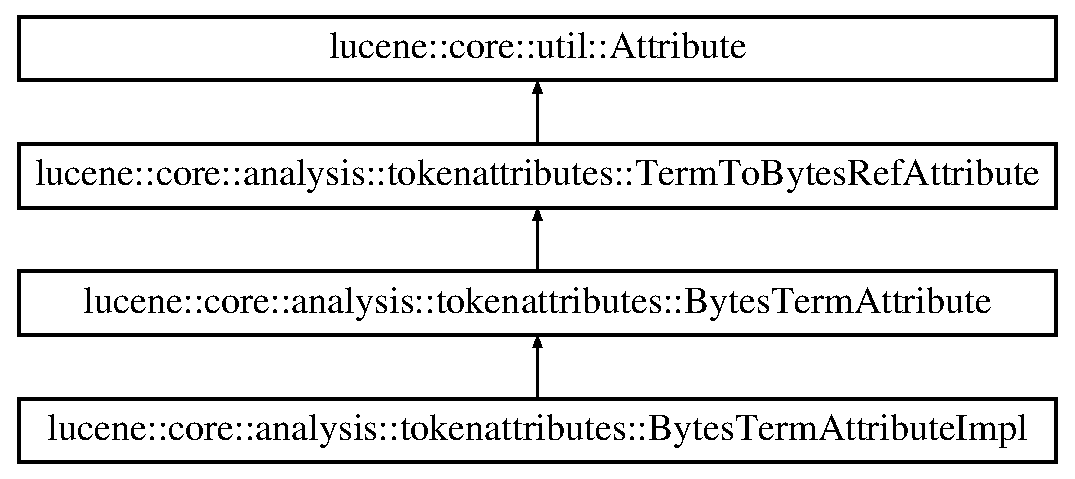
\includegraphics[height=4.000000cm]{classlucene_1_1core_1_1analysis_1_1tokenattributes_1_1BytesTermAttribute}
\end{center}
\end{figure}
\subsection*{Public Member Functions}
\begin{DoxyCompactItemize}
\item 
\mbox{\hyperlink{classlucene_1_1core_1_1analysis_1_1tokenattributes_1_1BytesTermAttribute_a96572fed858fc7b45f0fe36269e41afc}{Bytes\+Term\+Attribute}} ()
\item 
virtual \mbox{\hyperlink{classlucene_1_1core_1_1analysis_1_1tokenattributes_1_1BytesTermAttribute_aa8b2f75f5cb46ff154fba02323d0ae16}{$\sim$\+Bytes\+Term\+Attribute}} ()
\item 
virtual void \mbox{\hyperlink{classlucene_1_1core_1_1analysis_1_1tokenattributes_1_1BytesTermAttribute_ac0aafed04df791feabdc9771280110b9}{Set\+Bytes\+Ref}} (\mbox{\hyperlink{classlucene_1_1core_1_1util_1_1BytesRef}{lucene\+::core\+::util\+::\+Bytes\+Ref}} \&\mbox{\hyperlink{classlucene_1_1core_1_1analysis_1_1tokenattributes_1_1BytesTermAttribute_adf534bc1c061247d7802bdb765236b89}{bytes}})=0
\end{DoxyCompactItemize}
\subsection*{Private Attributes}
\begin{DoxyCompactItemize}
\item 
\mbox{\hyperlink{classlucene_1_1core_1_1util_1_1BytesRef}{lucene\+::core\+::util\+::\+Bytes\+Ref}} \mbox{\hyperlink{classlucene_1_1core_1_1analysis_1_1tokenattributes_1_1BytesTermAttribute_adf534bc1c061247d7802bdb765236b89}{bytes}}
\end{DoxyCompactItemize}
\subsection*{Additional Inherited Members}


\subsection{Constructor \& Destructor Documentation}
\mbox{\Hypertarget{classlucene_1_1core_1_1analysis_1_1tokenattributes_1_1BytesTermAttribute_a96572fed858fc7b45f0fe36269e41afc}\label{classlucene_1_1core_1_1analysis_1_1tokenattributes_1_1BytesTermAttribute_a96572fed858fc7b45f0fe36269e41afc}} 
\index{lucene\+::core\+::analysis\+::tokenattributes\+::\+Bytes\+Term\+Attribute@{lucene\+::core\+::analysis\+::tokenattributes\+::\+Bytes\+Term\+Attribute}!Bytes\+Term\+Attribute@{Bytes\+Term\+Attribute}}
\index{Bytes\+Term\+Attribute@{Bytes\+Term\+Attribute}!lucene\+::core\+::analysis\+::tokenattributes\+::\+Bytes\+Term\+Attribute@{lucene\+::core\+::analysis\+::tokenattributes\+::\+Bytes\+Term\+Attribute}}
\subsubsection{\texorpdfstring{Bytes\+Term\+Attribute()}{BytesTermAttribute()}}
{\footnotesize\ttfamily lucene\+::core\+::analysis\+::tokenattributes\+::\+Bytes\+Term\+Attribute\+::\+Bytes\+Term\+Attribute (\begin{DoxyParamCaption}{ }\end{DoxyParamCaption})\hspace{0.3cm}{\ttfamily [inline]}}

\mbox{\Hypertarget{classlucene_1_1core_1_1analysis_1_1tokenattributes_1_1BytesTermAttribute_aa8b2f75f5cb46ff154fba02323d0ae16}\label{classlucene_1_1core_1_1analysis_1_1tokenattributes_1_1BytesTermAttribute_aa8b2f75f5cb46ff154fba02323d0ae16}} 
\index{lucene\+::core\+::analysis\+::tokenattributes\+::\+Bytes\+Term\+Attribute@{lucene\+::core\+::analysis\+::tokenattributes\+::\+Bytes\+Term\+Attribute}!````~Bytes\+Term\+Attribute@{$\sim$\+Bytes\+Term\+Attribute}}
\index{````~Bytes\+Term\+Attribute@{$\sim$\+Bytes\+Term\+Attribute}!lucene\+::core\+::analysis\+::tokenattributes\+::\+Bytes\+Term\+Attribute@{lucene\+::core\+::analysis\+::tokenattributes\+::\+Bytes\+Term\+Attribute}}
\subsubsection{\texorpdfstring{$\sim$\+Bytes\+Term\+Attribute()}{~BytesTermAttribute()}}
{\footnotesize\ttfamily virtual lucene\+::core\+::analysis\+::tokenattributes\+::\+Bytes\+Term\+Attribute\+::$\sim$\+Bytes\+Term\+Attribute (\begin{DoxyParamCaption}{ }\end{DoxyParamCaption})\hspace{0.3cm}{\ttfamily [inline]}, {\ttfamily [virtual]}}



\subsection{Member Function Documentation}
\mbox{\Hypertarget{classlucene_1_1core_1_1analysis_1_1tokenattributes_1_1BytesTermAttribute_ac0aafed04df791feabdc9771280110b9}\label{classlucene_1_1core_1_1analysis_1_1tokenattributes_1_1BytesTermAttribute_ac0aafed04df791feabdc9771280110b9}} 
\index{lucene\+::core\+::analysis\+::tokenattributes\+::\+Bytes\+Term\+Attribute@{lucene\+::core\+::analysis\+::tokenattributes\+::\+Bytes\+Term\+Attribute}!Set\+Bytes\+Ref@{Set\+Bytes\+Ref}}
\index{Set\+Bytes\+Ref@{Set\+Bytes\+Ref}!lucene\+::core\+::analysis\+::tokenattributes\+::\+Bytes\+Term\+Attribute@{lucene\+::core\+::analysis\+::tokenattributes\+::\+Bytes\+Term\+Attribute}}
\subsubsection{\texorpdfstring{Set\+Bytes\+Ref()}{SetBytesRef()}}
{\footnotesize\ttfamily virtual void lucene\+::core\+::analysis\+::tokenattributes\+::\+Bytes\+Term\+Attribute\+::\+Set\+Bytes\+Ref (\begin{DoxyParamCaption}\item[{\mbox{\hyperlink{classlucene_1_1core_1_1util_1_1BytesRef}{lucene\+::core\+::util\+::\+Bytes\+Ref}} \&}]{bytes }\end{DoxyParamCaption})\hspace{0.3cm}{\ttfamily [pure virtual]}}



Implemented in \mbox{\hyperlink{classlucene_1_1core_1_1analysis_1_1tokenattributes_1_1BytesTermAttributeImpl_a132152487a88eae5feb1f88543d08c65}{lucene\+::core\+::analysis\+::tokenattributes\+::\+Bytes\+Term\+Attribute\+Impl}}.



\subsection{Member Data Documentation}
\mbox{\Hypertarget{classlucene_1_1core_1_1analysis_1_1tokenattributes_1_1BytesTermAttribute_adf534bc1c061247d7802bdb765236b89}\label{classlucene_1_1core_1_1analysis_1_1tokenattributes_1_1BytesTermAttribute_adf534bc1c061247d7802bdb765236b89}} 
\index{lucene\+::core\+::analysis\+::tokenattributes\+::\+Bytes\+Term\+Attribute@{lucene\+::core\+::analysis\+::tokenattributes\+::\+Bytes\+Term\+Attribute}!bytes@{bytes}}
\index{bytes@{bytes}!lucene\+::core\+::analysis\+::tokenattributes\+::\+Bytes\+Term\+Attribute@{lucene\+::core\+::analysis\+::tokenattributes\+::\+Bytes\+Term\+Attribute}}
\subsubsection{\texorpdfstring{bytes}{bytes}}
{\footnotesize\ttfamily \mbox{\hyperlink{classlucene_1_1core_1_1util_1_1BytesRef}{lucene\+::core\+::util\+::\+Bytes\+Ref}} lucene\+::core\+::analysis\+::tokenattributes\+::\+Bytes\+Term\+Attribute\+::bytes\hspace{0.3cm}{\ttfamily [private]}}



The documentation for this class was generated from the following file\+:\begin{DoxyCompactItemize}
\item 
Analysis/\mbox{\hyperlink{Analysis_2Attribute_8h}{Attribute.\+h}}\end{DoxyCompactItemize}

\hypertarget{classlucene_1_1core_1_1analysis_1_1tokenattributes_1_1BytesTermAttributeImpl}{}\section{lucene\+:\+:core\+:\+:analysis\+:\+:tokenattributes\+:\+:Bytes\+Term\+Attribute\+Impl Class Reference}
\label{classlucene_1_1core_1_1analysis_1_1tokenattributes_1_1BytesTermAttributeImpl}\index{lucene\+::core\+::analysis\+::tokenattributes\+::\+Bytes\+Term\+Attribute\+Impl@{lucene\+::core\+::analysis\+::tokenattributes\+::\+Bytes\+Term\+Attribute\+Impl}}


{\ttfamily \#include $<$Attribute\+Impl.\+h$>$}

Inheritance diagram for lucene\+:\+:core\+:\+:analysis\+:\+:tokenattributes\+:\+:Bytes\+Term\+Attribute\+Impl\+:\begin{figure}[H]
\begin{center}
\leavevmode
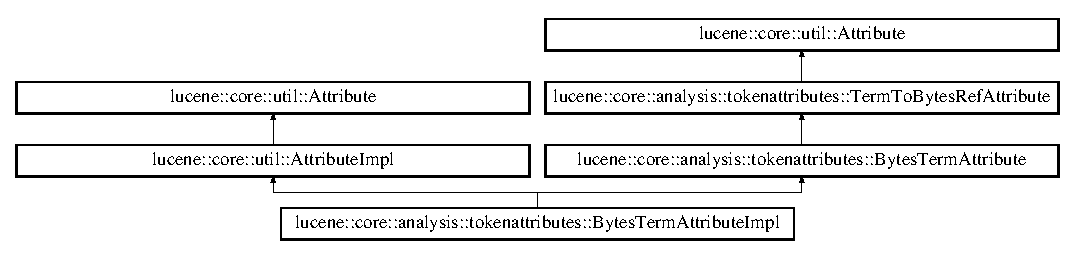
\includegraphics[height=2.994652cm]{classlucene_1_1core_1_1analysis_1_1tokenattributes_1_1BytesTermAttributeImpl}
\end{center}
\end{figure}
\subsection*{Public Member Functions}
\begin{DoxyCompactItemize}
\item 
\mbox{\hyperlink{classlucene_1_1core_1_1analysis_1_1tokenattributes_1_1BytesTermAttributeImpl_a615b3f72279153190787e471fcf1e550}{Bytes\+Term\+Attribute\+Impl}} ()
\item 
\mbox{\hyperlink{classlucene_1_1core_1_1analysis_1_1tokenattributes_1_1BytesTermAttributeImpl_a7fa1f130126d96924101d3ab9716f921}{Bytes\+Term\+Attribute\+Impl}} (\mbox{\hyperlink{ZlibCrc32_8h_a2c212835823e3c54a8ab6d95c652660e}{const}} \mbox{\hyperlink{classlucene_1_1core_1_1analysis_1_1tokenattributes_1_1BytesTermAttributeImpl}{Bytes\+Term\+Attribute\+Impl}} \&other)
\item 
\mbox{\hyperlink{classlucene_1_1core_1_1util_1_1BytesRef}{lucene\+::core\+::util\+::\+Bytes\+Ref}} \& \mbox{\hyperlink{classlucene_1_1core_1_1analysis_1_1tokenattributes_1_1BytesTermAttributeImpl_ab0c78ee232b1546b553118afc0117374}{Get\+Bytes\+Ref}} () override
\item 
virtual \mbox{\hyperlink{classlucene_1_1core_1_1analysis_1_1tokenattributes_1_1BytesTermAttributeImpl_a03844cda01d3357b0e60ae4424fafc33}{$\sim$\+Bytes\+Term\+Attribute\+Impl}} ()
\item 
void \mbox{\hyperlink{classlucene_1_1core_1_1analysis_1_1tokenattributes_1_1BytesTermAttributeImpl_a132152487a88eae5feb1f88543d08c65}{Set\+Bytes\+Ref}} (\mbox{\hyperlink{classlucene_1_1core_1_1util_1_1BytesRef}{lucene\+::core\+::util\+::\+Bytes\+Ref}} \&\mbox{\hyperlink{classlucene_1_1core_1_1analysis_1_1tokenattributes_1_1BytesTermAttributeImpl_aedd53d552069d367ff2ede8111ce1944}{bytes}}) override
\item 
void \mbox{\hyperlink{classlucene_1_1core_1_1analysis_1_1tokenattributes_1_1BytesTermAttributeImpl_a6fa48596a507c937bd874d46ef5ca963}{Clear}} () override
\item 
void \mbox{\hyperlink{classlucene_1_1core_1_1analysis_1_1tokenattributes_1_1BytesTermAttributeImpl_a6a1789244604f807529de975d4c10171}{Reflect\+With}} (\mbox{\hyperlink{namespacelucene_1_1core_1_1util_a7dbb701adaed055f73fb95eec83da10a}{lucene\+::core\+::util\+::\+Attribute\+Reflector}} \&reflector) override
\item 
bool \mbox{\hyperlink{classlucene_1_1core_1_1analysis_1_1tokenattributes_1_1BytesTermAttributeImpl_a7cb94efc8c682f0caf2bca4f0ffb2981}{operator==}} (\mbox{\hyperlink{ZlibCrc32_8h_a2c212835823e3c54a8ab6d95c652660e}{const}} \mbox{\hyperlink{classlucene_1_1core_1_1analysis_1_1tokenattributes_1_1BytesTermAttributeImpl}{Bytes\+Term\+Attribute\+Impl}} \&other) \mbox{\hyperlink{ZlibCrc32_8h_a2c212835823e3c54a8ab6d95c652660e}{const}}
\item 
std\+::vector$<$ std\+::type\+\_\+index $>$ \mbox{\hyperlink{classlucene_1_1core_1_1analysis_1_1tokenattributes_1_1BytesTermAttributeImpl_aff915b815335534889b45fa2ce773692}{Attributes}} () override
\item 
void \mbox{\hyperlink{classlucene_1_1core_1_1analysis_1_1tokenattributes_1_1BytesTermAttributeImpl_aafc25a873ed04661a26d6a7b5f6d2b0d}{Shallow\+Copy\+To}} (\mbox{\hyperlink{classlucene_1_1core_1_1util_1_1AttributeImpl}{lucene\+::core\+::util\+::\+Attribute\+Impl}} \&attr\+\_\+impl) override
\item 
\mbox{\hyperlink{classlucene_1_1core_1_1analysis_1_1tokenattributes_1_1BytesTermAttributeImpl}{Bytes\+Term\+Attribute\+Impl}} \& \mbox{\hyperlink{classlucene_1_1core_1_1analysis_1_1tokenattributes_1_1BytesTermAttributeImpl_acfaef15f10ddfec3e2494c6d2176ac73}{operator=}} (\mbox{\hyperlink{ZlibCrc32_8h_a2c212835823e3c54a8ab6d95c652660e}{const}} \mbox{\hyperlink{classlucene_1_1core_1_1util_1_1AttributeImpl}{lucene\+::core\+::util\+::\+Attribute\+Impl}} \&other)
\item 
\mbox{\hyperlink{classlucene_1_1core_1_1analysis_1_1tokenattributes_1_1BytesTermAttributeImpl}{Bytes\+Term\+Attribute\+Impl}} \& \mbox{\hyperlink{classlucene_1_1core_1_1analysis_1_1tokenattributes_1_1BytesTermAttributeImpl_a3d91c14505c1b59ea0372697b87c79f6}{operator=}} (\mbox{\hyperlink{ZlibCrc32_8h_a2c212835823e3c54a8ab6d95c652660e}{const}} \mbox{\hyperlink{classlucene_1_1core_1_1analysis_1_1tokenattributes_1_1BytesTermAttributeImpl}{Bytes\+Term\+Attribute\+Impl}} \&other)
\item 
\mbox{\hyperlink{classlucene_1_1core_1_1util_1_1AttributeImpl}{lucene\+::core\+::util\+::\+Attribute\+Impl}} $\ast$ \mbox{\hyperlink{classlucene_1_1core_1_1analysis_1_1tokenattributes_1_1BytesTermAttributeImpl_a149760a0122009e6b699862553d43b41}{Clone}} () override
\end{DoxyCompactItemize}
\subsection*{Private Attributes}
\begin{DoxyCompactItemize}
\item 
\mbox{\hyperlink{classlucene_1_1core_1_1util_1_1BytesRef}{lucene\+::core\+::util\+::\+Bytes\+Ref}} \mbox{\hyperlink{classlucene_1_1core_1_1analysis_1_1tokenattributes_1_1BytesTermAttributeImpl_aedd53d552069d367ff2ede8111ce1944}{bytes}}
\end{DoxyCompactItemize}
\subsection*{Additional Inherited Members}


\subsection{Constructor \& Destructor Documentation}
\mbox{\Hypertarget{classlucene_1_1core_1_1analysis_1_1tokenattributes_1_1BytesTermAttributeImpl_a615b3f72279153190787e471fcf1e550}\label{classlucene_1_1core_1_1analysis_1_1tokenattributes_1_1BytesTermAttributeImpl_a615b3f72279153190787e471fcf1e550}} 
\index{lucene\+::core\+::analysis\+::tokenattributes\+::\+Bytes\+Term\+Attribute\+Impl@{lucene\+::core\+::analysis\+::tokenattributes\+::\+Bytes\+Term\+Attribute\+Impl}!Bytes\+Term\+Attribute\+Impl@{Bytes\+Term\+Attribute\+Impl}}
\index{Bytes\+Term\+Attribute\+Impl@{Bytes\+Term\+Attribute\+Impl}!lucene\+::core\+::analysis\+::tokenattributes\+::\+Bytes\+Term\+Attribute\+Impl@{lucene\+::core\+::analysis\+::tokenattributes\+::\+Bytes\+Term\+Attribute\+Impl}}
\subsubsection{\texorpdfstring{Bytes\+Term\+Attribute\+Impl()}{BytesTermAttributeImpl()}\hspace{0.1cm}{\footnotesize\ttfamily [1/2]}}
{\footnotesize\ttfamily Bytes\+Term\+Attribute\+Impl\+::\+Bytes\+Term\+Attribute\+Impl (\begin{DoxyParamCaption}{ }\end{DoxyParamCaption})}

\mbox{\hyperlink{classlucene_1_1core_1_1analysis_1_1tokenattributes_1_1BytesTermAttributeImpl}{Bytes\+Term\+Attribute\+Impl}} \mbox{\Hypertarget{classlucene_1_1core_1_1analysis_1_1tokenattributes_1_1BytesTermAttributeImpl_a7fa1f130126d96924101d3ab9716f921}\label{classlucene_1_1core_1_1analysis_1_1tokenattributes_1_1BytesTermAttributeImpl_a7fa1f130126d96924101d3ab9716f921}} 
\index{lucene\+::core\+::analysis\+::tokenattributes\+::\+Bytes\+Term\+Attribute\+Impl@{lucene\+::core\+::analysis\+::tokenattributes\+::\+Bytes\+Term\+Attribute\+Impl}!Bytes\+Term\+Attribute\+Impl@{Bytes\+Term\+Attribute\+Impl}}
\index{Bytes\+Term\+Attribute\+Impl@{Bytes\+Term\+Attribute\+Impl}!lucene\+::core\+::analysis\+::tokenattributes\+::\+Bytes\+Term\+Attribute\+Impl@{lucene\+::core\+::analysis\+::tokenattributes\+::\+Bytes\+Term\+Attribute\+Impl}}
\subsubsection{\texorpdfstring{Bytes\+Term\+Attribute\+Impl()}{BytesTermAttributeImpl()}\hspace{0.1cm}{\footnotesize\ttfamily [2/2]}}
{\footnotesize\ttfamily Bytes\+Term\+Attribute\+Impl\+::\+Bytes\+Term\+Attribute\+Impl (\begin{DoxyParamCaption}\item[{\mbox{\hyperlink{ZlibCrc32_8h_a2c212835823e3c54a8ab6d95c652660e}{const}} \mbox{\hyperlink{classlucene_1_1core_1_1analysis_1_1tokenattributes_1_1BytesTermAttributeImpl}{Bytes\+Term\+Attribute\+Impl}} \&}]{other }\end{DoxyParamCaption})}

\mbox{\Hypertarget{classlucene_1_1core_1_1analysis_1_1tokenattributes_1_1BytesTermAttributeImpl_a03844cda01d3357b0e60ae4424fafc33}\label{classlucene_1_1core_1_1analysis_1_1tokenattributes_1_1BytesTermAttributeImpl_a03844cda01d3357b0e60ae4424fafc33}} 
\index{lucene\+::core\+::analysis\+::tokenattributes\+::\+Bytes\+Term\+Attribute\+Impl@{lucene\+::core\+::analysis\+::tokenattributes\+::\+Bytes\+Term\+Attribute\+Impl}!````~Bytes\+Term\+Attribute\+Impl@{$\sim$\+Bytes\+Term\+Attribute\+Impl}}
\index{````~Bytes\+Term\+Attribute\+Impl@{$\sim$\+Bytes\+Term\+Attribute\+Impl}!lucene\+::core\+::analysis\+::tokenattributes\+::\+Bytes\+Term\+Attribute\+Impl@{lucene\+::core\+::analysis\+::tokenattributes\+::\+Bytes\+Term\+Attribute\+Impl}}
\subsubsection{\texorpdfstring{$\sim$\+Bytes\+Term\+Attribute\+Impl()}{~BytesTermAttributeImpl()}}
{\footnotesize\ttfamily Bytes\+Term\+Attribute\+Impl\+::$\sim$\+Bytes\+Term\+Attribute\+Impl (\begin{DoxyParamCaption}{ }\end{DoxyParamCaption})\hspace{0.3cm}{\ttfamily [virtual]}}



\subsection{Member Function Documentation}
\mbox{\Hypertarget{classlucene_1_1core_1_1analysis_1_1tokenattributes_1_1BytesTermAttributeImpl_aff915b815335534889b45fa2ce773692}\label{classlucene_1_1core_1_1analysis_1_1tokenattributes_1_1BytesTermAttributeImpl_aff915b815335534889b45fa2ce773692}} 
\index{lucene\+::core\+::analysis\+::tokenattributes\+::\+Bytes\+Term\+Attribute\+Impl@{lucene\+::core\+::analysis\+::tokenattributes\+::\+Bytes\+Term\+Attribute\+Impl}!Attributes@{Attributes}}
\index{Attributes@{Attributes}!lucene\+::core\+::analysis\+::tokenattributes\+::\+Bytes\+Term\+Attribute\+Impl@{lucene\+::core\+::analysis\+::tokenattributes\+::\+Bytes\+Term\+Attribute\+Impl}}
\subsubsection{\texorpdfstring{Attributes()}{Attributes()}}
{\footnotesize\ttfamily std\+::vector$<$ std\+::type\+\_\+index $>$ Bytes\+Term\+Attribute\+Impl\+::\+Attributes (\begin{DoxyParamCaption}{ }\end{DoxyParamCaption})\hspace{0.3cm}{\ttfamily [override]}, {\ttfamily [virtual]}}



Implements \mbox{\hyperlink{classlucene_1_1core_1_1util_1_1AttributeImpl_ac0631e6a7a11044883bc97447716d7cc}{lucene\+::core\+::util\+::\+Attribute\+Impl}}.

\mbox{\Hypertarget{classlucene_1_1core_1_1analysis_1_1tokenattributes_1_1BytesTermAttributeImpl_a6fa48596a507c937bd874d46ef5ca963}\label{classlucene_1_1core_1_1analysis_1_1tokenattributes_1_1BytesTermAttributeImpl_a6fa48596a507c937bd874d46ef5ca963}} 
\index{lucene\+::core\+::analysis\+::tokenattributes\+::\+Bytes\+Term\+Attribute\+Impl@{lucene\+::core\+::analysis\+::tokenattributes\+::\+Bytes\+Term\+Attribute\+Impl}!Clear@{Clear}}
\index{Clear@{Clear}!lucene\+::core\+::analysis\+::tokenattributes\+::\+Bytes\+Term\+Attribute\+Impl@{lucene\+::core\+::analysis\+::tokenattributes\+::\+Bytes\+Term\+Attribute\+Impl}}
\subsubsection{\texorpdfstring{Clear()}{Clear()}}
{\footnotesize\ttfamily void Bytes\+Term\+Attribute\+Impl\+::\+Clear (\begin{DoxyParamCaption}{ }\end{DoxyParamCaption})\hspace{0.3cm}{\ttfamily [override]}, {\ttfamily [virtual]}}



Implements \mbox{\hyperlink{classlucene_1_1core_1_1util_1_1AttributeImpl_a04897a00a902f7a345dd44bbc4b482a8}{lucene\+::core\+::util\+::\+Attribute\+Impl}}.

\mbox{\Hypertarget{classlucene_1_1core_1_1analysis_1_1tokenattributes_1_1BytesTermAttributeImpl_a149760a0122009e6b699862553d43b41}\label{classlucene_1_1core_1_1analysis_1_1tokenattributes_1_1BytesTermAttributeImpl_a149760a0122009e6b699862553d43b41}} 
\index{lucene\+::core\+::analysis\+::tokenattributes\+::\+Bytes\+Term\+Attribute\+Impl@{lucene\+::core\+::analysis\+::tokenattributes\+::\+Bytes\+Term\+Attribute\+Impl}!Clone@{Clone}}
\index{Clone@{Clone}!lucene\+::core\+::analysis\+::tokenattributes\+::\+Bytes\+Term\+Attribute\+Impl@{lucene\+::core\+::analysis\+::tokenattributes\+::\+Bytes\+Term\+Attribute\+Impl}}
\subsubsection{\texorpdfstring{Clone()}{Clone()}}
{\footnotesize\ttfamily \mbox{\hyperlink{classlucene_1_1core_1_1util_1_1AttributeImpl}{Attribute\+Impl}} $\ast$ Bytes\+Term\+Attribute\+Impl\+::\+Clone (\begin{DoxyParamCaption}{ }\end{DoxyParamCaption})\hspace{0.3cm}{\ttfamily [override]}, {\ttfamily [virtual]}}



Implements \mbox{\hyperlink{classlucene_1_1core_1_1util_1_1AttributeImpl_a135318ad4c7c17b3d85e625e32fb42cd}{lucene\+::core\+::util\+::\+Attribute\+Impl}}.

\mbox{\Hypertarget{classlucene_1_1core_1_1analysis_1_1tokenattributes_1_1BytesTermAttributeImpl_ab0c78ee232b1546b553118afc0117374}\label{classlucene_1_1core_1_1analysis_1_1tokenattributes_1_1BytesTermAttributeImpl_ab0c78ee232b1546b553118afc0117374}} 
\index{lucene\+::core\+::analysis\+::tokenattributes\+::\+Bytes\+Term\+Attribute\+Impl@{lucene\+::core\+::analysis\+::tokenattributes\+::\+Bytes\+Term\+Attribute\+Impl}!Get\+Bytes\+Ref@{Get\+Bytes\+Ref}}
\index{Get\+Bytes\+Ref@{Get\+Bytes\+Ref}!lucene\+::core\+::analysis\+::tokenattributes\+::\+Bytes\+Term\+Attribute\+Impl@{lucene\+::core\+::analysis\+::tokenattributes\+::\+Bytes\+Term\+Attribute\+Impl}}
\subsubsection{\texorpdfstring{Get\+Bytes\+Ref()}{GetBytesRef()}}
{\footnotesize\ttfamily \mbox{\hyperlink{classlucene_1_1core_1_1util_1_1BytesRef}{Bytes\+Ref}} \& Bytes\+Term\+Attribute\+Impl\+::\+Get\+Bytes\+Ref (\begin{DoxyParamCaption}{ }\end{DoxyParamCaption})\hspace{0.3cm}{\ttfamily [override]}, {\ttfamily [virtual]}}



Implements \mbox{\hyperlink{classlucene_1_1core_1_1analysis_1_1tokenattributes_1_1TermToBytesRefAttribute_a8ae9e4cfc1b97185f8151f3eac76a20d}{lucene\+::core\+::analysis\+::tokenattributes\+::\+Term\+To\+Bytes\+Ref\+Attribute}}.

\mbox{\Hypertarget{classlucene_1_1core_1_1analysis_1_1tokenattributes_1_1BytesTermAttributeImpl_acfaef15f10ddfec3e2494c6d2176ac73}\label{classlucene_1_1core_1_1analysis_1_1tokenattributes_1_1BytesTermAttributeImpl_acfaef15f10ddfec3e2494c6d2176ac73}} 
\index{lucene\+::core\+::analysis\+::tokenattributes\+::\+Bytes\+Term\+Attribute\+Impl@{lucene\+::core\+::analysis\+::tokenattributes\+::\+Bytes\+Term\+Attribute\+Impl}!operator=@{operator=}}
\index{operator=@{operator=}!lucene\+::core\+::analysis\+::tokenattributes\+::\+Bytes\+Term\+Attribute\+Impl@{lucene\+::core\+::analysis\+::tokenattributes\+::\+Bytes\+Term\+Attribute\+Impl}}
\subsubsection{\texorpdfstring{operator=()}{operator=()}\hspace{0.1cm}{\footnotesize\ttfamily [1/2]}}
{\footnotesize\ttfamily \mbox{\hyperlink{classlucene_1_1core_1_1analysis_1_1tokenattributes_1_1BytesTermAttributeImpl}{Bytes\+Term\+Attribute\+Impl}} \& Bytes\+Term\+Attribute\+Impl\+::operator= (\begin{DoxyParamCaption}\item[{\mbox{\hyperlink{ZlibCrc32_8h_a2c212835823e3c54a8ab6d95c652660e}{const}} \mbox{\hyperlink{classlucene_1_1core_1_1util_1_1AttributeImpl}{lucene\+::core\+::util\+::\+Attribute\+Impl}} \&}]{other }\end{DoxyParamCaption})\hspace{0.3cm}{\ttfamily [virtual]}}



Implements \mbox{\hyperlink{classlucene_1_1core_1_1util_1_1AttributeImpl_ab032e399d03ce2f58c76881cf2b92325}{lucene\+::core\+::util\+::\+Attribute\+Impl}}.

\mbox{\Hypertarget{classlucene_1_1core_1_1analysis_1_1tokenattributes_1_1BytesTermAttributeImpl_a3d91c14505c1b59ea0372697b87c79f6}\label{classlucene_1_1core_1_1analysis_1_1tokenattributes_1_1BytesTermAttributeImpl_a3d91c14505c1b59ea0372697b87c79f6}} 
\index{lucene\+::core\+::analysis\+::tokenattributes\+::\+Bytes\+Term\+Attribute\+Impl@{lucene\+::core\+::analysis\+::tokenattributes\+::\+Bytes\+Term\+Attribute\+Impl}!operator=@{operator=}}
\index{operator=@{operator=}!lucene\+::core\+::analysis\+::tokenattributes\+::\+Bytes\+Term\+Attribute\+Impl@{lucene\+::core\+::analysis\+::tokenattributes\+::\+Bytes\+Term\+Attribute\+Impl}}
\subsubsection{\texorpdfstring{operator=()}{operator=()}\hspace{0.1cm}{\footnotesize\ttfamily [2/2]}}
{\footnotesize\ttfamily \mbox{\hyperlink{classlucene_1_1core_1_1analysis_1_1tokenattributes_1_1BytesTermAttributeImpl}{Bytes\+Term\+Attribute\+Impl}} \& Bytes\+Term\+Attribute\+Impl\+::operator= (\begin{DoxyParamCaption}\item[{\mbox{\hyperlink{ZlibCrc32_8h_a2c212835823e3c54a8ab6d95c652660e}{const}} \mbox{\hyperlink{classlucene_1_1core_1_1analysis_1_1tokenattributes_1_1BytesTermAttributeImpl}{Bytes\+Term\+Attribute\+Impl}} \&}]{other }\end{DoxyParamCaption})}

\mbox{\Hypertarget{classlucene_1_1core_1_1analysis_1_1tokenattributes_1_1BytesTermAttributeImpl_a7cb94efc8c682f0caf2bca4f0ffb2981}\label{classlucene_1_1core_1_1analysis_1_1tokenattributes_1_1BytesTermAttributeImpl_a7cb94efc8c682f0caf2bca4f0ffb2981}} 
\index{lucene\+::core\+::analysis\+::tokenattributes\+::\+Bytes\+Term\+Attribute\+Impl@{lucene\+::core\+::analysis\+::tokenattributes\+::\+Bytes\+Term\+Attribute\+Impl}!operator==@{operator==}}
\index{operator==@{operator==}!lucene\+::core\+::analysis\+::tokenattributes\+::\+Bytes\+Term\+Attribute\+Impl@{lucene\+::core\+::analysis\+::tokenattributes\+::\+Bytes\+Term\+Attribute\+Impl}}
\subsubsection{\texorpdfstring{operator==()}{operator==()}}
{\footnotesize\ttfamily bool Bytes\+Term\+Attribute\+Impl\+::operator== (\begin{DoxyParamCaption}\item[{\mbox{\hyperlink{ZlibCrc32_8h_a2c212835823e3c54a8ab6d95c652660e}{const}} \mbox{\hyperlink{classlucene_1_1core_1_1analysis_1_1tokenattributes_1_1BytesTermAttributeImpl}{Bytes\+Term\+Attribute\+Impl}} \&}]{other }\end{DoxyParamCaption}) const}

\mbox{\Hypertarget{classlucene_1_1core_1_1analysis_1_1tokenattributes_1_1BytesTermAttributeImpl_a6a1789244604f807529de975d4c10171}\label{classlucene_1_1core_1_1analysis_1_1tokenattributes_1_1BytesTermAttributeImpl_a6a1789244604f807529de975d4c10171}} 
\index{lucene\+::core\+::analysis\+::tokenattributes\+::\+Bytes\+Term\+Attribute\+Impl@{lucene\+::core\+::analysis\+::tokenattributes\+::\+Bytes\+Term\+Attribute\+Impl}!Reflect\+With@{Reflect\+With}}
\index{Reflect\+With@{Reflect\+With}!lucene\+::core\+::analysis\+::tokenattributes\+::\+Bytes\+Term\+Attribute\+Impl@{lucene\+::core\+::analysis\+::tokenattributes\+::\+Bytes\+Term\+Attribute\+Impl}}
\subsubsection{\texorpdfstring{Reflect\+With()}{ReflectWith()}}
{\footnotesize\ttfamily void Bytes\+Term\+Attribute\+Impl\+::\+Reflect\+With (\begin{DoxyParamCaption}\item[{\mbox{\hyperlink{namespacelucene_1_1core_1_1util_a7dbb701adaed055f73fb95eec83da10a}{lucene\+::core\+::util\+::\+Attribute\+Reflector}} \&}]{reflector }\end{DoxyParamCaption})\hspace{0.3cm}{\ttfamily [override]}, {\ttfamily [virtual]}}



Implements \mbox{\hyperlink{classlucene_1_1core_1_1util_1_1AttributeImpl_a84d34275fb1ed67ac36fad7ff6388096}{lucene\+::core\+::util\+::\+Attribute\+Impl}}.

\mbox{\Hypertarget{classlucene_1_1core_1_1analysis_1_1tokenattributes_1_1BytesTermAttributeImpl_a132152487a88eae5feb1f88543d08c65}\label{classlucene_1_1core_1_1analysis_1_1tokenattributes_1_1BytesTermAttributeImpl_a132152487a88eae5feb1f88543d08c65}} 
\index{lucene\+::core\+::analysis\+::tokenattributes\+::\+Bytes\+Term\+Attribute\+Impl@{lucene\+::core\+::analysis\+::tokenattributes\+::\+Bytes\+Term\+Attribute\+Impl}!Set\+Bytes\+Ref@{Set\+Bytes\+Ref}}
\index{Set\+Bytes\+Ref@{Set\+Bytes\+Ref}!lucene\+::core\+::analysis\+::tokenattributes\+::\+Bytes\+Term\+Attribute\+Impl@{lucene\+::core\+::analysis\+::tokenattributes\+::\+Bytes\+Term\+Attribute\+Impl}}
\subsubsection{\texorpdfstring{Set\+Bytes\+Ref()}{SetBytesRef()}}
{\footnotesize\ttfamily void Bytes\+Term\+Attribute\+Impl\+::\+Set\+Bytes\+Ref (\begin{DoxyParamCaption}\item[{\mbox{\hyperlink{classlucene_1_1core_1_1util_1_1BytesRef}{lucene\+::core\+::util\+::\+Bytes\+Ref}} \&}]{bytes }\end{DoxyParamCaption})\hspace{0.3cm}{\ttfamily [override]}, {\ttfamily [virtual]}}



Implements \mbox{\hyperlink{classlucene_1_1core_1_1analysis_1_1tokenattributes_1_1BytesTermAttribute_ac0aafed04df791feabdc9771280110b9}{lucene\+::core\+::analysis\+::tokenattributes\+::\+Bytes\+Term\+Attribute}}.

\mbox{\Hypertarget{classlucene_1_1core_1_1analysis_1_1tokenattributes_1_1BytesTermAttributeImpl_aafc25a873ed04661a26d6a7b5f6d2b0d}\label{classlucene_1_1core_1_1analysis_1_1tokenattributes_1_1BytesTermAttributeImpl_aafc25a873ed04661a26d6a7b5f6d2b0d}} 
\index{lucene\+::core\+::analysis\+::tokenattributes\+::\+Bytes\+Term\+Attribute\+Impl@{lucene\+::core\+::analysis\+::tokenattributes\+::\+Bytes\+Term\+Attribute\+Impl}!Shallow\+Copy\+To@{Shallow\+Copy\+To}}
\index{Shallow\+Copy\+To@{Shallow\+Copy\+To}!lucene\+::core\+::analysis\+::tokenattributes\+::\+Bytes\+Term\+Attribute\+Impl@{lucene\+::core\+::analysis\+::tokenattributes\+::\+Bytes\+Term\+Attribute\+Impl}}
\subsubsection{\texorpdfstring{Shallow\+Copy\+To()}{ShallowCopyTo()}}
{\footnotesize\ttfamily void Bytes\+Term\+Attribute\+Impl\+::\+Shallow\+Copy\+To (\begin{DoxyParamCaption}\item[{\mbox{\hyperlink{classlucene_1_1core_1_1util_1_1AttributeImpl}{lucene\+::core\+::util\+::\+Attribute\+Impl}} \&}]{attr\+\_\+impl }\end{DoxyParamCaption})\hspace{0.3cm}{\ttfamily [override]}, {\ttfamily [virtual]}}



Implements \mbox{\hyperlink{classlucene_1_1core_1_1util_1_1AttributeImpl_a010e8937832f53139c8fe42757476895}{lucene\+::core\+::util\+::\+Attribute\+Impl}}.



\subsection{Member Data Documentation}
\mbox{\Hypertarget{classlucene_1_1core_1_1analysis_1_1tokenattributes_1_1BytesTermAttributeImpl_aedd53d552069d367ff2ede8111ce1944}\label{classlucene_1_1core_1_1analysis_1_1tokenattributes_1_1BytesTermAttributeImpl_aedd53d552069d367ff2ede8111ce1944}} 
\index{lucene\+::core\+::analysis\+::tokenattributes\+::\+Bytes\+Term\+Attribute\+Impl@{lucene\+::core\+::analysis\+::tokenattributes\+::\+Bytes\+Term\+Attribute\+Impl}!bytes@{bytes}}
\index{bytes@{bytes}!lucene\+::core\+::analysis\+::tokenattributes\+::\+Bytes\+Term\+Attribute\+Impl@{lucene\+::core\+::analysis\+::tokenattributes\+::\+Bytes\+Term\+Attribute\+Impl}}
\subsubsection{\texorpdfstring{bytes}{bytes}}
{\footnotesize\ttfamily \mbox{\hyperlink{classlucene_1_1core_1_1util_1_1BytesRef}{lucene\+::core\+::util\+::\+Bytes\+Ref}} lucene\+::core\+::analysis\+::tokenattributes\+::\+Bytes\+Term\+Attribute\+Impl\+::bytes\hspace{0.3cm}{\ttfamily [private]}}



The documentation for this class was generated from the following files\+:\begin{DoxyCompactItemize}
\item 
Analysis/\mbox{\hyperlink{AttributeImpl_8h}{Attribute\+Impl.\+h}}\item 
Analysis/\mbox{\hyperlink{AttributeImpl_8cpp}{Attribute\+Impl.\+cpp}}\end{DoxyCompactItemize}

\hypertarget{classlucene_1_1core_1_1analysis_1_1CachingTokenFilter}{}\section{lucene\+:\+:core\+:\+:analysis\+:\+:Caching\+Token\+Filter Class Reference}
\label{classlucene_1_1core_1_1analysis_1_1CachingTokenFilter}\index{lucene\+::core\+::analysis\+::\+Caching\+Token\+Filter@{lucene\+::core\+::analysis\+::\+Caching\+Token\+Filter}}


{\ttfamily \#include $<$Token\+Stream.\+h$>$}

Inheritance diagram for lucene\+:\+:core\+:\+:analysis\+:\+:Caching\+Token\+Filter\+:\begin{figure}[H]
\begin{center}
\leavevmode
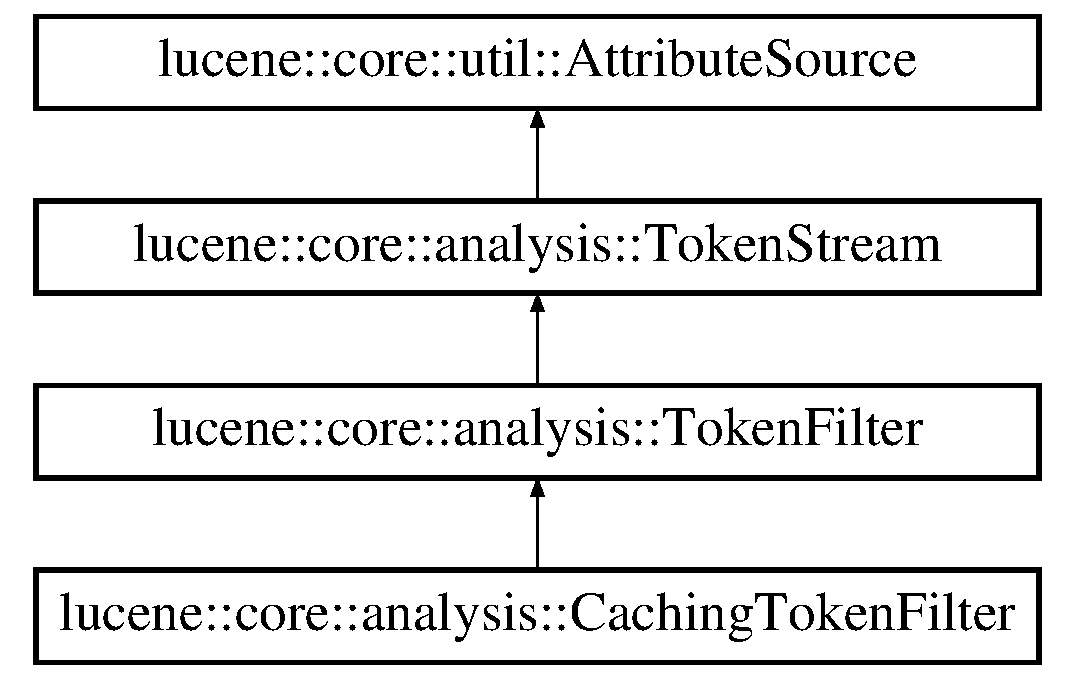
\includegraphics[height=4.000000cm]{classlucene_1_1core_1_1analysis_1_1CachingTokenFilter}
\end{center}
\end{figure}
\subsection*{Public Member Functions}
\begin{DoxyCompactItemize}
\item 
\mbox{\hyperlink{classlucene_1_1core_1_1analysis_1_1CachingTokenFilter_acbcb907639dbeeb5fc0f9925b804438f}{Caching\+Token\+Filter}} (std\+::shared\+\_\+ptr$<$ \mbox{\hyperlink{classlucene_1_1core_1_1analysis_1_1TokenStream}{Token\+Stream}} $>$ in)
\item 
\mbox{\hyperlink{classlucene_1_1core_1_1analysis_1_1CachingTokenFilter_ae15751d487684a8d3b0835b69fd8f976}{Caching\+Token\+Filter}} (\mbox{\hyperlink{classlucene_1_1core_1_1analysis_1_1TokenStream}{Token\+Stream}} $\ast$in)
\item 
virtual \mbox{\hyperlink{classlucene_1_1core_1_1analysis_1_1CachingTokenFilter_acbad05f7b0c43c2be38c616c7dbe3dfa}{$\sim$\+Caching\+Token\+Filter}} ()
\item 
void \mbox{\hyperlink{classlucene_1_1core_1_1analysis_1_1CachingTokenFilter_a7241be5e51e730f4e311572510de147e}{End}} () override
\item 
void \mbox{\hyperlink{classlucene_1_1core_1_1analysis_1_1CachingTokenFilter_adde877fb8c464d6eb2766bd400a1499c}{Reset}} () override
\item 
bool \mbox{\hyperlink{classlucene_1_1core_1_1analysis_1_1CachingTokenFilter_acea0a0a5ee61ab8831209c96fde49dc8}{Increment\+Token}} () override
\end{DoxyCompactItemize}
\subsection*{Private Member Functions}
\begin{DoxyCompactItemize}
\item 
void \mbox{\hyperlink{classlucene_1_1core_1_1analysis_1_1CachingTokenFilter_a9c3602a328bb00156c13ae278cac5f3a}{Fill\+Cache}} ()
\item 
bool \mbox{\hyperlink{classlucene_1_1core_1_1analysis_1_1CachingTokenFilter_accc1b57932239f41fd7d97594da49722}{Is\+Cached}} ()
\end{DoxyCompactItemize}
\subsection*{Private Attributes}
\begin{DoxyCompactItemize}
\item 
std\+::vector$<$ std\+::unique\+\_\+ptr$<$ \mbox{\hyperlink{classlucene_1_1core_1_1util_1_1AttributeSource_1_1State}{lucene\+::core\+::util\+::\+Attribute\+Source\+::\+State}} $>$ $>$ \mbox{\hyperlink{classlucene_1_1core_1_1analysis_1_1CachingTokenFilter_a84d2af768b782d2ba4eb2c4ebc095d1d}{cache}}
\item 
std\+::vector$<$ std\+::unique\+\_\+ptr$<$ \mbox{\hyperlink{classlucene_1_1core_1_1util_1_1AttributeSource_1_1State}{lucene\+::core\+::util\+::\+Attribute\+Source\+::\+State}} $>$ $>$\+::iterator \mbox{\hyperlink{classlucene_1_1core_1_1analysis_1_1CachingTokenFilter_a23615478893652578c8cab6ca5275ff3}{iterator}}
\item 
std\+::unique\+\_\+ptr$<$ \mbox{\hyperlink{classlucene_1_1core_1_1util_1_1AttributeSource_1_1State}{lucene\+::core\+::util\+::\+Attribute\+Source\+::\+State}} $>$ \mbox{\hyperlink{classlucene_1_1core_1_1analysis_1_1CachingTokenFilter_a843e6f3b087cb20663ffbd995266704f}{final\+\_\+state}}
\item 
bool \mbox{\hyperlink{classlucene_1_1core_1_1analysis_1_1CachingTokenFilter_aea35743bf279c67214d8567e6230ed4c}{first\+\_\+time}}
\end{DoxyCompactItemize}
\subsection*{Additional Inherited Members}


\subsection{Constructor \& Destructor Documentation}
\mbox{\Hypertarget{classlucene_1_1core_1_1analysis_1_1CachingTokenFilter_acbcb907639dbeeb5fc0f9925b804438f}\label{classlucene_1_1core_1_1analysis_1_1CachingTokenFilter_acbcb907639dbeeb5fc0f9925b804438f}} 
\index{lucene\+::core\+::analysis\+::\+Caching\+Token\+Filter@{lucene\+::core\+::analysis\+::\+Caching\+Token\+Filter}!Caching\+Token\+Filter@{Caching\+Token\+Filter}}
\index{Caching\+Token\+Filter@{Caching\+Token\+Filter}!lucene\+::core\+::analysis\+::\+Caching\+Token\+Filter@{lucene\+::core\+::analysis\+::\+Caching\+Token\+Filter}}
\subsubsection{\texorpdfstring{Caching\+Token\+Filter()}{CachingTokenFilter()}\hspace{0.1cm}{\footnotesize\ttfamily [1/2]}}
{\footnotesize\ttfamily lucene\+::core\+::analysis\+::\+Caching\+Token\+Filter\+::\+Caching\+Token\+Filter (\begin{DoxyParamCaption}\item[{std\+::shared\+\_\+ptr$<$ \mbox{\hyperlink{classlucene_1_1core_1_1analysis_1_1TokenStream}{Token\+Stream}} $>$}]{in }\end{DoxyParamCaption})\hspace{0.3cm}{\ttfamily [explicit]}}

\mbox{\Hypertarget{classlucene_1_1core_1_1analysis_1_1CachingTokenFilter_ae15751d487684a8d3b0835b69fd8f976}\label{classlucene_1_1core_1_1analysis_1_1CachingTokenFilter_ae15751d487684a8d3b0835b69fd8f976}} 
\index{lucene\+::core\+::analysis\+::\+Caching\+Token\+Filter@{lucene\+::core\+::analysis\+::\+Caching\+Token\+Filter}!Caching\+Token\+Filter@{Caching\+Token\+Filter}}
\index{Caching\+Token\+Filter@{Caching\+Token\+Filter}!lucene\+::core\+::analysis\+::\+Caching\+Token\+Filter@{lucene\+::core\+::analysis\+::\+Caching\+Token\+Filter}}
\subsubsection{\texorpdfstring{Caching\+Token\+Filter()}{CachingTokenFilter()}\hspace{0.1cm}{\footnotesize\ttfamily [2/2]}}
{\footnotesize\ttfamily Caching\+Token\+Filter\+::\+Caching\+Token\+Filter (\begin{DoxyParamCaption}\item[{\mbox{\hyperlink{classlucene_1_1core_1_1analysis_1_1TokenStream}{Token\+Stream}} $\ast$}]{in }\end{DoxyParamCaption})\hspace{0.3cm}{\ttfamily [explicit]}}

\mbox{\hyperlink{classlucene_1_1core_1_1analysis_1_1CachingTokenFilter}{Caching\+Token\+Filter}} \mbox{\Hypertarget{classlucene_1_1core_1_1analysis_1_1CachingTokenFilter_acbad05f7b0c43c2be38c616c7dbe3dfa}\label{classlucene_1_1core_1_1analysis_1_1CachingTokenFilter_acbad05f7b0c43c2be38c616c7dbe3dfa}} 
\index{lucene\+::core\+::analysis\+::\+Caching\+Token\+Filter@{lucene\+::core\+::analysis\+::\+Caching\+Token\+Filter}!````~Caching\+Token\+Filter@{$\sim$\+Caching\+Token\+Filter}}
\index{````~Caching\+Token\+Filter@{$\sim$\+Caching\+Token\+Filter}!lucene\+::core\+::analysis\+::\+Caching\+Token\+Filter@{lucene\+::core\+::analysis\+::\+Caching\+Token\+Filter}}
\subsubsection{\texorpdfstring{$\sim$\+Caching\+Token\+Filter()}{~CachingTokenFilter()}}
{\footnotesize\ttfamily Caching\+Token\+Filter\+::$\sim$\+Caching\+Token\+Filter (\begin{DoxyParamCaption}{ }\end{DoxyParamCaption})\hspace{0.3cm}{\ttfamily [virtual]}}



\subsection{Member Function Documentation}
\mbox{\Hypertarget{classlucene_1_1core_1_1analysis_1_1CachingTokenFilter_a7241be5e51e730f4e311572510de147e}\label{classlucene_1_1core_1_1analysis_1_1CachingTokenFilter_a7241be5e51e730f4e311572510de147e}} 
\index{lucene\+::core\+::analysis\+::\+Caching\+Token\+Filter@{lucene\+::core\+::analysis\+::\+Caching\+Token\+Filter}!End@{End}}
\index{End@{End}!lucene\+::core\+::analysis\+::\+Caching\+Token\+Filter@{lucene\+::core\+::analysis\+::\+Caching\+Token\+Filter}}
\subsubsection{\texorpdfstring{End()}{End()}}
{\footnotesize\ttfamily void Caching\+Token\+Filter\+::\+End (\begin{DoxyParamCaption}{ }\end{DoxyParamCaption})\hspace{0.3cm}{\ttfamily [override]}, {\ttfamily [virtual]}}



Reimplemented from \mbox{\hyperlink{classlucene_1_1core_1_1analysis_1_1TokenFilter_ad2e29dd32aa4df385d0f290f10f20721}{lucene\+::core\+::analysis\+::\+Token\+Filter}}.

\mbox{\Hypertarget{classlucene_1_1core_1_1analysis_1_1CachingTokenFilter_a9c3602a328bb00156c13ae278cac5f3a}\label{classlucene_1_1core_1_1analysis_1_1CachingTokenFilter_a9c3602a328bb00156c13ae278cac5f3a}} 
\index{lucene\+::core\+::analysis\+::\+Caching\+Token\+Filter@{lucene\+::core\+::analysis\+::\+Caching\+Token\+Filter}!Fill\+Cache@{Fill\+Cache}}
\index{Fill\+Cache@{Fill\+Cache}!lucene\+::core\+::analysis\+::\+Caching\+Token\+Filter@{lucene\+::core\+::analysis\+::\+Caching\+Token\+Filter}}
\subsubsection{\texorpdfstring{Fill\+Cache()}{FillCache()}}
{\footnotesize\ttfamily void Caching\+Token\+Filter\+::\+Fill\+Cache (\begin{DoxyParamCaption}{ }\end{DoxyParamCaption})\hspace{0.3cm}{\ttfamily [private]}}

\mbox{\Hypertarget{classlucene_1_1core_1_1analysis_1_1CachingTokenFilter_acea0a0a5ee61ab8831209c96fde49dc8}\label{classlucene_1_1core_1_1analysis_1_1CachingTokenFilter_acea0a0a5ee61ab8831209c96fde49dc8}} 
\index{lucene\+::core\+::analysis\+::\+Caching\+Token\+Filter@{lucene\+::core\+::analysis\+::\+Caching\+Token\+Filter}!Increment\+Token@{Increment\+Token}}
\index{Increment\+Token@{Increment\+Token}!lucene\+::core\+::analysis\+::\+Caching\+Token\+Filter@{lucene\+::core\+::analysis\+::\+Caching\+Token\+Filter}}
\subsubsection{\texorpdfstring{Increment\+Token()}{IncrementToken()}}
{\footnotesize\ttfamily bool Caching\+Token\+Filter\+::\+Increment\+Token (\begin{DoxyParamCaption}{ }\end{DoxyParamCaption})\hspace{0.3cm}{\ttfamily [override]}, {\ttfamily [virtual]}}



Implements \mbox{\hyperlink{classlucene_1_1core_1_1analysis_1_1TokenStream_a614d4ea24a354d6f4354b4941b5124e2}{lucene\+::core\+::analysis\+::\+Token\+Stream}}.

\mbox{\Hypertarget{classlucene_1_1core_1_1analysis_1_1CachingTokenFilter_accc1b57932239f41fd7d97594da49722}\label{classlucene_1_1core_1_1analysis_1_1CachingTokenFilter_accc1b57932239f41fd7d97594da49722}} 
\index{lucene\+::core\+::analysis\+::\+Caching\+Token\+Filter@{lucene\+::core\+::analysis\+::\+Caching\+Token\+Filter}!Is\+Cached@{Is\+Cached}}
\index{Is\+Cached@{Is\+Cached}!lucene\+::core\+::analysis\+::\+Caching\+Token\+Filter@{lucene\+::core\+::analysis\+::\+Caching\+Token\+Filter}}
\subsubsection{\texorpdfstring{Is\+Cached()}{IsCached()}}
{\footnotesize\ttfamily bool Caching\+Token\+Filter\+::\+Is\+Cached (\begin{DoxyParamCaption}{ }\end{DoxyParamCaption})\hspace{0.3cm}{\ttfamily [private]}}

\mbox{\Hypertarget{classlucene_1_1core_1_1analysis_1_1CachingTokenFilter_adde877fb8c464d6eb2766bd400a1499c}\label{classlucene_1_1core_1_1analysis_1_1CachingTokenFilter_adde877fb8c464d6eb2766bd400a1499c}} 
\index{lucene\+::core\+::analysis\+::\+Caching\+Token\+Filter@{lucene\+::core\+::analysis\+::\+Caching\+Token\+Filter}!Reset@{Reset}}
\index{Reset@{Reset}!lucene\+::core\+::analysis\+::\+Caching\+Token\+Filter@{lucene\+::core\+::analysis\+::\+Caching\+Token\+Filter}}
\subsubsection{\texorpdfstring{Reset()}{Reset()}}
{\footnotesize\ttfamily void Caching\+Token\+Filter\+::\+Reset (\begin{DoxyParamCaption}{ }\end{DoxyParamCaption})\hspace{0.3cm}{\ttfamily [override]}, {\ttfamily [virtual]}}



Reimplemented from \mbox{\hyperlink{classlucene_1_1core_1_1analysis_1_1TokenFilter_a0671ee825db7735a7b72b7a27a457ed9}{lucene\+::core\+::analysis\+::\+Token\+Filter}}.



\subsection{Member Data Documentation}
\mbox{\Hypertarget{classlucene_1_1core_1_1analysis_1_1CachingTokenFilter_a84d2af768b782d2ba4eb2c4ebc095d1d}\label{classlucene_1_1core_1_1analysis_1_1CachingTokenFilter_a84d2af768b782d2ba4eb2c4ebc095d1d}} 
\index{lucene\+::core\+::analysis\+::\+Caching\+Token\+Filter@{lucene\+::core\+::analysis\+::\+Caching\+Token\+Filter}!cache@{cache}}
\index{cache@{cache}!lucene\+::core\+::analysis\+::\+Caching\+Token\+Filter@{lucene\+::core\+::analysis\+::\+Caching\+Token\+Filter}}
\subsubsection{\texorpdfstring{cache}{cache}}
{\footnotesize\ttfamily std\+::vector$<$std\+::unique\+\_\+ptr$<$\mbox{\hyperlink{classlucene_1_1core_1_1util_1_1AttributeSource_1_1State}{lucene\+::core\+::util\+::\+Attribute\+Source\+::\+State}}$>$ $>$ lucene\+::core\+::analysis\+::\+Caching\+Token\+Filter\+::cache\hspace{0.3cm}{\ttfamily [private]}}

\mbox{\Hypertarget{classlucene_1_1core_1_1analysis_1_1CachingTokenFilter_a843e6f3b087cb20663ffbd995266704f}\label{classlucene_1_1core_1_1analysis_1_1CachingTokenFilter_a843e6f3b087cb20663ffbd995266704f}} 
\index{lucene\+::core\+::analysis\+::\+Caching\+Token\+Filter@{lucene\+::core\+::analysis\+::\+Caching\+Token\+Filter}!final\+\_\+state@{final\+\_\+state}}
\index{final\+\_\+state@{final\+\_\+state}!lucene\+::core\+::analysis\+::\+Caching\+Token\+Filter@{lucene\+::core\+::analysis\+::\+Caching\+Token\+Filter}}
\subsubsection{\texorpdfstring{final\+\_\+state}{final\_state}}
{\footnotesize\ttfamily std\+::unique\+\_\+ptr$<$\mbox{\hyperlink{classlucene_1_1core_1_1util_1_1AttributeSource_1_1State}{lucene\+::core\+::util\+::\+Attribute\+Source\+::\+State}}$>$ lucene\+::core\+::analysis\+::\+Caching\+Token\+Filter\+::final\+\_\+state\hspace{0.3cm}{\ttfamily [private]}}

\mbox{\Hypertarget{classlucene_1_1core_1_1analysis_1_1CachingTokenFilter_aea35743bf279c67214d8567e6230ed4c}\label{classlucene_1_1core_1_1analysis_1_1CachingTokenFilter_aea35743bf279c67214d8567e6230ed4c}} 
\index{lucene\+::core\+::analysis\+::\+Caching\+Token\+Filter@{lucene\+::core\+::analysis\+::\+Caching\+Token\+Filter}!first\+\_\+time@{first\+\_\+time}}
\index{first\+\_\+time@{first\+\_\+time}!lucene\+::core\+::analysis\+::\+Caching\+Token\+Filter@{lucene\+::core\+::analysis\+::\+Caching\+Token\+Filter}}
\subsubsection{\texorpdfstring{first\+\_\+time}{first\_time}}
{\footnotesize\ttfamily bool lucene\+::core\+::analysis\+::\+Caching\+Token\+Filter\+::first\+\_\+time\hspace{0.3cm}{\ttfamily [private]}}

\mbox{\Hypertarget{classlucene_1_1core_1_1analysis_1_1CachingTokenFilter_a23615478893652578c8cab6ca5275ff3}\label{classlucene_1_1core_1_1analysis_1_1CachingTokenFilter_a23615478893652578c8cab6ca5275ff3}} 
\index{lucene\+::core\+::analysis\+::\+Caching\+Token\+Filter@{lucene\+::core\+::analysis\+::\+Caching\+Token\+Filter}!iterator@{iterator}}
\index{iterator@{iterator}!lucene\+::core\+::analysis\+::\+Caching\+Token\+Filter@{lucene\+::core\+::analysis\+::\+Caching\+Token\+Filter}}
\subsubsection{\texorpdfstring{iterator}{iterator}}
{\footnotesize\ttfamily std\+::vector$<$std\+::unique\+\_\+ptr$<$\mbox{\hyperlink{classlucene_1_1core_1_1util_1_1AttributeSource_1_1State}{lucene\+::core\+::util\+::\+Attribute\+Source\+::\+State}}$>$ $>$\+::iterator lucene\+::core\+::analysis\+::\+Caching\+Token\+Filter\+::iterator\hspace{0.3cm}{\ttfamily [private]}}



The documentation for this class was generated from the following files\+:\begin{DoxyCompactItemize}
\item 
Analysis/\mbox{\hyperlink{TokenStream_8h}{Token\+Stream.\+h}}\item 
Analysis/\mbox{\hyperlink{TokenStream_8cpp}{Token\+Stream.\+cpp}}\end{DoxyCompactItemize}

\hypertarget{classlucene_1_1core_1_1analysis_1_1characterutil_1_1CharFilter}{}\section{lucene\+:\+:core\+:\+:analysis\+:\+:characterutil\+:\+:Char\+Filter Class Reference}
\label{classlucene_1_1core_1_1analysis_1_1characterutil_1_1CharFilter}\index{lucene\+::core\+::analysis\+::characterutil\+::\+Char\+Filter@{lucene\+::core\+::analysis\+::characterutil\+::\+Char\+Filter}}


{\ttfamily \#include $<$Character\+Util.\+h$>$}

Inheritance diagram for lucene\+:\+:core\+:\+:analysis\+:\+:characterutil\+:\+:Char\+Filter\+:\begin{figure}[H]
\begin{center}
\leavevmode
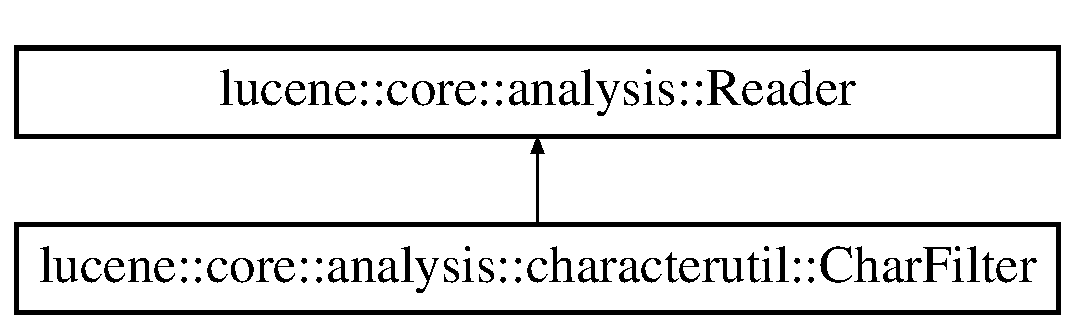
\includegraphics[height=2.000000cm]{classlucene_1_1core_1_1analysis_1_1characterutil_1_1CharFilter}
\end{center}
\end{figure}
\subsection*{Public Member Functions}
\begin{DoxyCompactItemize}
\item 
\mbox{\hyperlink{classlucene_1_1core_1_1analysis_1_1characterutil_1_1CharFilter_ac13b7526b15e97a551071c2b759d1af1}{Char\+Filter}} (\mbox{\hyperlink{classlucene_1_1core_1_1analysis_1_1Reader}{Reader}} $\ast$\mbox{\hyperlink{classlucene_1_1core_1_1analysis_1_1characterutil_1_1CharFilter_a774b34856b115721d2ec012e475413c4}{input}})
\item 
virtual \mbox{\hyperlink{classlucene_1_1core_1_1analysis_1_1characterutil_1_1CharFilter_acf60f32d245a97caebc76508363d61b6}{$\sim$\+Char\+Filter}} ()
\item 
void \mbox{\hyperlink{classlucene_1_1core_1_1analysis_1_1characterutil_1_1CharFilter_a47ff3dc61979b80927ed5779cb55bd09}{Close}} ()
\item 
virtual int32\+\_\+t \mbox{\hyperlink{classlucene_1_1core_1_1analysis_1_1characterutil_1_1CharFilter_ad1be13a08cf750862795cb9b29ed4e09}{Correct}} (const int32\+\_\+t current\+\_\+off)=0
\item 
int32\+\_\+t \mbox{\hyperlink{classlucene_1_1core_1_1analysis_1_1characterutil_1_1CharFilter_a6e4becb7161f99dec056ef207fda3f23}{Correct\+Offset}} (const int32\+\_\+t current\+\_\+off)
\end{DoxyCompactItemize}
\subsection*{Private Attributes}
\begin{DoxyCompactItemize}
\item 
std\+::unique\+\_\+ptr$<$ \mbox{\hyperlink{classlucene_1_1core_1_1analysis_1_1Reader}{Reader}} $>$ \mbox{\hyperlink{classlucene_1_1core_1_1analysis_1_1characterutil_1_1CharFilter_a774b34856b115721d2ec012e475413c4}{input}}
\end{DoxyCompactItemize}


\subsection{Constructor \& Destructor Documentation}
\mbox{\Hypertarget{classlucene_1_1core_1_1analysis_1_1characterutil_1_1CharFilter_ac13b7526b15e97a551071c2b759d1af1}\label{classlucene_1_1core_1_1analysis_1_1characterutil_1_1CharFilter_ac13b7526b15e97a551071c2b759d1af1}} 
\index{lucene\+::core\+::analysis\+::characterutil\+::\+Char\+Filter@{lucene\+::core\+::analysis\+::characterutil\+::\+Char\+Filter}!Char\+Filter@{Char\+Filter}}
\index{Char\+Filter@{Char\+Filter}!lucene\+::core\+::analysis\+::characterutil\+::\+Char\+Filter@{lucene\+::core\+::analysis\+::characterutil\+::\+Char\+Filter}}
\subsubsection{\texorpdfstring{Char\+Filter()}{CharFilter()}}
{\footnotesize\ttfamily Char\+Filter\+::\+Char\+Filter (\begin{DoxyParamCaption}\item[{\mbox{\hyperlink{classlucene_1_1core_1_1analysis_1_1Reader}{Reader}} $\ast$}]{input }\end{DoxyParamCaption})\hspace{0.3cm}{\ttfamily [explicit]}}

\mbox{\hyperlink{classlucene_1_1core_1_1analysis_1_1characterutil_1_1CharFilter}{Char\+Filter}}\textquotesingle{}s constructor. Given input reader is will be owned by \mbox{\hyperlink{classlucene_1_1core_1_1analysis_1_1characterutil_1_1CharFilter}{Char\+Filter}} instance

\mbox{\hyperlink{classlucene_1_1core_1_1analysis_1_1characterutil_1_1CharFilter}{Char\+Filter}} \mbox{\Hypertarget{classlucene_1_1core_1_1analysis_1_1characterutil_1_1CharFilter_acf60f32d245a97caebc76508363d61b6}\label{classlucene_1_1core_1_1analysis_1_1characterutil_1_1CharFilter_acf60f32d245a97caebc76508363d61b6}} 
\index{lucene\+::core\+::analysis\+::characterutil\+::\+Char\+Filter@{lucene\+::core\+::analysis\+::characterutil\+::\+Char\+Filter}!````~Char\+Filter@{$\sim$\+Char\+Filter}}
\index{````~Char\+Filter@{$\sim$\+Char\+Filter}!lucene\+::core\+::analysis\+::characterutil\+::\+Char\+Filter@{lucene\+::core\+::analysis\+::characterutil\+::\+Char\+Filter}}
\subsubsection{\texorpdfstring{$\sim$\+Char\+Filter()}{~CharFilter()}}
{\footnotesize\ttfamily Char\+Filter\+::$\sim$\+Char\+Filter (\begin{DoxyParamCaption}{ }\end{DoxyParamCaption})\hspace{0.3cm}{\ttfamily [virtual]}}



\subsection{Member Function Documentation}
\mbox{\Hypertarget{classlucene_1_1core_1_1analysis_1_1characterutil_1_1CharFilter_a47ff3dc61979b80927ed5779cb55bd09}\label{classlucene_1_1core_1_1analysis_1_1characterutil_1_1CharFilter_a47ff3dc61979b80927ed5779cb55bd09}} 
\index{lucene\+::core\+::analysis\+::characterutil\+::\+Char\+Filter@{lucene\+::core\+::analysis\+::characterutil\+::\+Char\+Filter}!Close@{Close}}
\index{Close@{Close}!lucene\+::core\+::analysis\+::characterutil\+::\+Char\+Filter@{lucene\+::core\+::analysis\+::characterutil\+::\+Char\+Filter}}
\subsubsection{\texorpdfstring{Close()}{Close()}}
{\footnotesize\ttfamily void Char\+Filter\+::\+Close (\begin{DoxyParamCaption}{ }\end{DoxyParamCaption})\hspace{0.3cm}{\ttfamily [virtual]}}



Implements \mbox{\hyperlink{classlucene_1_1core_1_1analysis_1_1Reader_a4be7e96dccdd3e276e3450e3ad7a70f4}{lucene\+::core\+::analysis\+::\+Reader}}.

\mbox{\Hypertarget{classlucene_1_1core_1_1analysis_1_1characterutil_1_1CharFilter_ad1be13a08cf750862795cb9b29ed4e09}\label{classlucene_1_1core_1_1analysis_1_1characterutil_1_1CharFilter_ad1be13a08cf750862795cb9b29ed4e09}} 
\index{lucene\+::core\+::analysis\+::characterutil\+::\+Char\+Filter@{lucene\+::core\+::analysis\+::characterutil\+::\+Char\+Filter}!Correct@{Correct}}
\index{Correct@{Correct}!lucene\+::core\+::analysis\+::characterutil\+::\+Char\+Filter@{lucene\+::core\+::analysis\+::characterutil\+::\+Char\+Filter}}
\subsubsection{\texorpdfstring{Correct()}{Correct()}}
{\footnotesize\ttfamily virtual int32\+\_\+t lucene\+::core\+::analysis\+::characterutil\+::\+Char\+Filter\+::\+Correct (\begin{DoxyParamCaption}\item[{const int32\+\_\+t}]{current\+\_\+off }\end{DoxyParamCaption})\hspace{0.3cm}{\ttfamily [pure virtual]}}

\mbox{\Hypertarget{classlucene_1_1core_1_1analysis_1_1characterutil_1_1CharFilter_a6e4becb7161f99dec056ef207fda3f23}\label{classlucene_1_1core_1_1analysis_1_1characterutil_1_1CharFilter_a6e4becb7161f99dec056ef207fda3f23}} 
\index{lucene\+::core\+::analysis\+::characterutil\+::\+Char\+Filter@{lucene\+::core\+::analysis\+::characterutil\+::\+Char\+Filter}!Correct\+Offset@{Correct\+Offset}}
\index{Correct\+Offset@{Correct\+Offset}!lucene\+::core\+::analysis\+::characterutil\+::\+Char\+Filter@{lucene\+::core\+::analysis\+::characterutil\+::\+Char\+Filter}}
\subsubsection{\texorpdfstring{Correct\+Offset()}{CorrectOffset()}}
{\footnotesize\ttfamily int32\+\_\+t Char\+Filter\+::\+Correct\+Offset (\begin{DoxyParamCaption}\item[{const int32\+\_\+t}]{current\+\_\+off }\end{DoxyParamCaption})}



\subsection{Member Data Documentation}
\mbox{\Hypertarget{classlucene_1_1core_1_1analysis_1_1characterutil_1_1CharFilter_a774b34856b115721d2ec012e475413c4}\label{classlucene_1_1core_1_1analysis_1_1characterutil_1_1CharFilter_a774b34856b115721d2ec012e475413c4}} 
\index{lucene\+::core\+::analysis\+::characterutil\+::\+Char\+Filter@{lucene\+::core\+::analysis\+::characterutil\+::\+Char\+Filter}!input@{input}}
\index{input@{input}!lucene\+::core\+::analysis\+::characterutil\+::\+Char\+Filter@{lucene\+::core\+::analysis\+::characterutil\+::\+Char\+Filter}}
\subsubsection{\texorpdfstring{input}{input}}
{\footnotesize\ttfamily std\+::unique\+\_\+ptr$<$\mbox{\hyperlink{classlucene_1_1core_1_1analysis_1_1Reader}{Reader}}$>$ lucene\+::core\+::analysis\+::characterutil\+::\+Char\+Filter\+::input\hspace{0.3cm}{\ttfamily [private]}}



The documentation for this class was generated from the following files\+:\begin{DoxyCompactItemize}
\item 
Analysis/\mbox{\hyperlink{CharacterUtil_8h}{Character\+Util.\+h}}\item 
Analysis/\mbox{\hyperlink{CharacterUtil_8cpp}{Character\+Util.\+cpp}}\end{DoxyCompactItemize}

\hypertarget{classlucene_1_1core_1_1analysis_1_1characterutil_1_1CharMap}{}\section{lucene\+:\+:core\+:\+:analysis\+:\+:characterutil\+:\+:Char\+Map$<$ V\+A\+L\+UE $>$ Class Template Reference}
\label{classlucene_1_1core_1_1analysis_1_1characterutil_1_1CharMap}\index{lucene\+::core\+::analysis\+::characterutil\+::\+Char\+Map$<$ V\+A\+L\+U\+E $>$@{lucene\+::core\+::analysis\+::characterutil\+::\+Char\+Map$<$ V\+A\+L\+U\+E $>$}}


{\ttfamily \#include $<$Character\+Util.\+h$>$}

\subsection*{Public Member Functions}
\begin{DoxyCompactItemize}
\item 
\mbox{\hyperlink{classlucene_1_1core_1_1analysis_1_1characterutil_1_1CharMap_ab593676daf8740d5f8394fabac807460}{Char\+Map}} (const bool \mbox{\hyperlink{classlucene_1_1core_1_1analysis_1_1characterutil_1_1CharMap_a1a62994159ecb2e6767c0d67238ad35c}{ignore\+\_\+case}}=false)
\item 
\mbox{\hyperlink{classlucene_1_1core_1_1analysis_1_1characterutil_1_1CharMap_a797c76287d00853e737c8fcd8006769d}{Char\+Map}} (const uint32\+\_\+t start\+\_\+size, const bool \mbox{\hyperlink{classlucene_1_1core_1_1analysis_1_1characterutil_1_1CharMap_a1a62994159ecb2e6767c0d67238ad35c}{ignore\+\_\+case}}=false)
\item 
{\footnotesize template$<$typename Input\+It $>$ }\\\mbox{\hyperlink{classlucene_1_1core_1_1analysis_1_1characterutil_1_1CharMap_a7449492bf51315ef11481821b113c0f1}{Char\+Map}} (Input\+It start, Input\+It end, const bool \mbox{\hyperlink{classlucene_1_1core_1_1analysis_1_1characterutil_1_1CharMap_a1a62994159ecb2e6767c0d67238ad35c}{ignore\+\_\+case}}=false)
\item 
\mbox{\hyperlink{classlucene_1_1core_1_1analysis_1_1characterutil_1_1CharMap_a0698d6cda30fd0a977a59ada5486f0b8}{Char\+Map}} (const \mbox{\hyperlink{classlucene_1_1core_1_1analysis_1_1characterutil_1_1CharMap}{Char\+Map}} \&other)
\item 
\mbox{\hyperlink{classlucene_1_1core_1_1analysis_1_1characterutil_1_1CharMap_aa83b5c7a819e10d002d8d06bc6ad45a0}{Char\+Map}} (const \mbox{\hyperlink{classlucene_1_1core_1_1analysis_1_1characterutil_1_1CharMap}{Char\+Map}} \&\&other)
\item 
\mbox{\hyperlink{classlucene_1_1core_1_1analysis_1_1characterutil_1_1CharMap_aa149df587eab8317179428d588f4829d}{$\sim$\+Char\+Map}} ()
\item 
\mbox{\hyperlink{classlucene_1_1core_1_1analysis_1_1characterutil_1_1CharMap}{Char\+Map}} \& \mbox{\hyperlink{classlucene_1_1core_1_1analysis_1_1characterutil_1_1CharMap_aabcf4f0d534fb6050aeb140d418a0fba}{operator=}} (const \mbox{\hyperlink{classlucene_1_1core_1_1analysis_1_1characterutil_1_1CharMap}{Char\+Map}} \&other)
\item 
\mbox{\hyperlink{classlucene_1_1core_1_1analysis_1_1characterutil_1_1CharMap}{Char\+Map}} \& \mbox{\hyperlink{classlucene_1_1core_1_1analysis_1_1characterutil_1_1CharMap_adef93a87f617af2b3f949b40ffd82cca}{operator=}} (const \mbox{\hyperlink{classlucene_1_1core_1_1analysis_1_1characterutil_1_1CharMap}{Char\+Map}} \&\&other)
\item 
void \mbox{\hyperlink{classlucene_1_1core_1_1analysis_1_1characterutil_1_1CharMap_aa8eb8edcee9f2d66b238baba7ddae641}{Clear}} ()
\item 
bool \mbox{\hyperlink{classlucene_1_1core_1_1analysis_1_1characterutil_1_1CharMap_a3c99e09a343372fdf0bbadd782e841ce}{Ignore\+Case}} ()
\item 
bool \mbox{\hyperlink{classlucene_1_1core_1_1analysis_1_1characterutil_1_1CharMap_a3ddc016640b2f1328eb4ccb68d11cc62}{Contains\+Key}} (const std\+::string \&str)
\item 
bool \mbox{\hyperlink{classlucene_1_1core_1_1analysis_1_1characterutil_1_1CharMap_a81b1167446c7c8988a523446436a313c}{Contains\+Key}} (const char $\ast$str, uint32\+\_\+t offset, uint32\+\_\+t length)
\item 
I\+N\+T\+E\+R\+N\+A\+L\+\_\+\+M\+A\+P\+::iterator \mbox{\hyperlink{classlucene_1_1core_1_1analysis_1_1characterutil_1_1CharMap_a48f8b551ec74f77bfbf6e53649d7ce74}{Get}} (const char $\ast$str, uint32\+\_\+t offset, uint32\+\_\+t length)
\item 
I\+N\+T\+E\+R\+N\+A\+L\+\_\+\+M\+A\+P\+::iterator \mbox{\hyperlink{classlucene_1_1core_1_1analysis_1_1characterutil_1_1CharMap_a753765dd29bb5f8c81ddb6b77d4cfa78}{Get}} (const std\+::string \&str)
\item 
bool \mbox{\hyperlink{classlucene_1_1core_1_1analysis_1_1characterutil_1_1CharMap_a09382e34715068e50efa4b40a34a4ee5}{Put}} (const char $\ast$str, uint32\+\_\+t offset, uint32\+\_\+t length, V\+A\+L\+UE \&value)
\item 
bool \mbox{\hyperlink{classlucene_1_1core_1_1analysis_1_1characterutil_1_1CharMap_a3d7b46fba00e762804ba1e953ac6587d}{Put}} (const char $\ast$str, uint32\+\_\+t offset, uint32\+\_\+t length, V\+A\+L\+UE \&\&value)
\item 
bool \mbox{\hyperlink{classlucene_1_1core_1_1analysis_1_1characterutil_1_1CharMap_aa93ef6c5bfec74a0533a9cd967adfc59}{Put}} (const std\+::string \&str, V\+A\+L\+UE \&value)
\item 
bool \mbox{\hyperlink{classlucene_1_1core_1_1analysis_1_1characterutil_1_1CharMap_a72fcb8b83852bb787de1204635d3bf21}{Put}} (const std\+::string \&str, V\+A\+L\+UE \&\&value)
\item 
bool \mbox{\hyperlink{classlucene_1_1core_1_1analysis_1_1characterutil_1_1CharMap_aa6267a07cdbe6c0d52c02ddad71c52ab}{Erase}} (const std\+::string \&str)
\item 
uint32\+\_\+t \mbox{\hyperlink{classlucene_1_1core_1_1analysis_1_1characterutil_1_1CharMap_a25bb4efe350f8848e264f63daf72f23e}{Size}} ()
\item 
I\+N\+T\+E\+R\+N\+A\+L\+\_\+\+M\+A\+P\+::iterator \mbox{\hyperlink{classlucene_1_1core_1_1analysis_1_1characterutil_1_1CharMap_a468af607829ccc32601ebb45c1363c7e}{Begin}} ()
\item 
I\+N\+T\+E\+R\+N\+A\+L\+\_\+\+M\+A\+P\+::iterator \mbox{\hyperlink{classlucene_1_1core_1_1analysis_1_1characterutil_1_1CharMap_a036c1820bceb5120f18a798b46db10d0}{End}} ()
\end{DoxyCompactItemize}
\subsection*{Private Types}
\begin{DoxyCompactItemize}
\item 
using \mbox{\hyperlink{classlucene_1_1core_1_1analysis_1_1characterutil_1_1CharMap_a0fe744ab48aa6f998a3d7e159a351d69}{I\+N\+T\+E\+R\+N\+A\+L\+\_\+\+M\+AP}} = std\+::unordered\+\_\+map$<$ \mbox{\hyperlink{classlucene_1_1core_1_1analysis_1_1characterutil_1_1CharPtrRangeInfo}{Char\+Ptr\+Range\+Info}}, V\+A\+L\+UE, \mbox{\hyperlink{classlucene_1_1core_1_1analysis_1_1characterutil_1_1CharPtrRangeInfoHasher}{Char\+Ptr\+Range\+Info\+Hasher}}, \mbox{\hyperlink{classlucene_1_1core_1_1analysis_1_1characterutil_1_1CharPtrRangeInfoEqual}{Char\+Ptr\+Range\+Info\+Equal}} $>$
\end{DoxyCompactItemize}
\subsection*{Private Attributes}
\begin{DoxyCompactItemize}
\item 
bool \mbox{\hyperlink{classlucene_1_1core_1_1analysis_1_1characterutil_1_1CharMap_a1a62994159ecb2e6767c0d67238ad35c}{ignore\+\_\+case}}
\item 
\mbox{\hyperlink{classlucene_1_1core_1_1analysis_1_1characterutil_1_1CharMap_a0fe744ab48aa6f998a3d7e159a351d69}{I\+N\+T\+E\+R\+N\+A\+L\+\_\+\+M\+AP}} \mbox{\hyperlink{classlucene_1_1core_1_1analysis_1_1characterutil_1_1CharMap_aa86d94ea61970d00283d8eb72d12e1cf}{internal\+\_\+map}}
\end{DoxyCompactItemize}


\subsection{Member Typedef Documentation}
\mbox{\Hypertarget{classlucene_1_1core_1_1analysis_1_1characterutil_1_1CharMap_a0fe744ab48aa6f998a3d7e159a351d69}\label{classlucene_1_1core_1_1analysis_1_1characterutil_1_1CharMap_a0fe744ab48aa6f998a3d7e159a351d69}} 
\index{lucene\+::core\+::analysis\+::characterutil\+::\+Char\+Map@{lucene\+::core\+::analysis\+::characterutil\+::\+Char\+Map}!I\+N\+T\+E\+R\+N\+A\+L\+\_\+\+M\+AP@{I\+N\+T\+E\+R\+N\+A\+L\+\_\+\+M\+AP}}
\index{I\+N\+T\+E\+R\+N\+A\+L\+\_\+\+M\+AP@{I\+N\+T\+E\+R\+N\+A\+L\+\_\+\+M\+AP}!lucene\+::core\+::analysis\+::characterutil\+::\+Char\+Map@{lucene\+::core\+::analysis\+::characterutil\+::\+Char\+Map}}
\subsubsection{\texorpdfstring{I\+N\+T\+E\+R\+N\+A\+L\+\_\+\+M\+AP}{INTERNAL\_MAP}}
{\footnotesize\ttfamily template$<$typename V\+A\+L\+UE$>$ \\
using \mbox{\hyperlink{classlucene_1_1core_1_1analysis_1_1characterutil_1_1CharMap}{lucene\+::core\+::analysis\+::characterutil\+::\+Char\+Map}}$<$ V\+A\+L\+UE $>$\+::\mbox{\hyperlink{classlucene_1_1core_1_1analysis_1_1characterutil_1_1CharMap_a0fe744ab48aa6f998a3d7e159a351d69}{I\+N\+T\+E\+R\+N\+A\+L\+\_\+\+M\+AP}} =  std\+::unordered\+\_\+map$<$\mbox{\hyperlink{classlucene_1_1core_1_1analysis_1_1characterutil_1_1CharPtrRangeInfo}{Char\+Ptr\+Range\+Info}}, V\+A\+L\+UE, \mbox{\hyperlink{classlucene_1_1core_1_1analysis_1_1characterutil_1_1CharPtrRangeInfoHasher}{Char\+Ptr\+Range\+Info\+Hasher}}, \mbox{\hyperlink{classlucene_1_1core_1_1analysis_1_1characterutil_1_1CharPtrRangeInfoEqual}{Char\+Ptr\+Range\+Info\+Equal}}$>$\hspace{0.3cm}{\ttfamily [private]}}



\subsection{Constructor \& Destructor Documentation}
\mbox{\Hypertarget{classlucene_1_1core_1_1analysis_1_1characterutil_1_1CharMap_ab593676daf8740d5f8394fabac807460}\label{classlucene_1_1core_1_1analysis_1_1characterutil_1_1CharMap_ab593676daf8740d5f8394fabac807460}} 
\index{lucene\+::core\+::analysis\+::characterutil\+::\+Char\+Map@{lucene\+::core\+::analysis\+::characterutil\+::\+Char\+Map}!Char\+Map@{Char\+Map}}
\index{Char\+Map@{Char\+Map}!lucene\+::core\+::analysis\+::characterutil\+::\+Char\+Map@{lucene\+::core\+::analysis\+::characterutil\+::\+Char\+Map}}
\subsubsection{\texorpdfstring{Char\+Map()}{CharMap()}\hspace{0.1cm}{\footnotesize\ttfamily [1/5]}}
{\footnotesize\ttfamily template$<$typename V\+A\+L\+UE$>$ \\
\mbox{\hyperlink{classlucene_1_1core_1_1analysis_1_1characterutil_1_1CharMap}{lucene\+::core\+::analysis\+::characterutil\+::\+Char\+Map}}$<$ V\+A\+L\+UE $>$\+::\mbox{\hyperlink{classlucene_1_1core_1_1analysis_1_1characterutil_1_1CharMap}{Char\+Map}} (\begin{DoxyParamCaption}\item[{const bool}]{ignore\+\_\+case = {\ttfamily false} }\end{DoxyParamCaption})\hspace{0.3cm}{\ttfamily [inline]}, {\ttfamily [explicit]}}

\mbox{\Hypertarget{classlucene_1_1core_1_1analysis_1_1characterutil_1_1CharMap_a797c76287d00853e737c8fcd8006769d}\label{classlucene_1_1core_1_1analysis_1_1characterutil_1_1CharMap_a797c76287d00853e737c8fcd8006769d}} 
\index{lucene\+::core\+::analysis\+::characterutil\+::\+Char\+Map@{lucene\+::core\+::analysis\+::characterutil\+::\+Char\+Map}!Char\+Map@{Char\+Map}}
\index{Char\+Map@{Char\+Map}!lucene\+::core\+::analysis\+::characterutil\+::\+Char\+Map@{lucene\+::core\+::analysis\+::characterutil\+::\+Char\+Map}}
\subsubsection{\texorpdfstring{Char\+Map()}{CharMap()}\hspace{0.1cm}{\footnotesize\ttfamily [2/5]}}
{\footnotesize\ttfamily template$<$typename V\+A\+L\+UE$>$ \\
\mbox{\hyperlink{classlucene_1_1core_1_1analysis_1_1characterutil_1_1CharMap}{lucene\+::core\+::analysis\+::characterutil\+::\+Char\+Map}}$<$ V\+A\+L\+UE $>$\+::\mbox{\hyperlink{classlucene_1_1core_1_1analysis_1_1characterutil_1_1CharMap}{Char\+Map}} (\begin{DoxyParamCaption}\item[{const uint32\+\_\+t}]{start\+\_\+size,  }\item[{const bool}]{ignore\+\_\+case = {\ttfamily false} }\end{DoxyParamCaption})\hspace{0.3cm}{\ttfamily [inline]}, {\ttfamily [explicit]}}

\mbox{\Hypertarget{classlucene_1_1core_1_1analysis_1_1characterutil_1_1CharMap_a7449492bf51315ef11481821b113c0f1}\label{classlucene_1_1core_1_1analysis_1_1characterutil_1_1CharMap_a7449492bf51315ef11481821b113c0f1}} 
\index{lucene\+::core\+::analysis\+::characterutil\+::\+Char\+Map@{lucene\+::core\+::analysis\+::characterutil\+::\+Char\+Map}!Char\+Map@{Char\+Map}}
\index{Char\+Map@{Char\+Map}!lucene\+::core\+::analysis\+::characterutil\+::\+Char\+Map@{lucene\+::core\+::analysis\+::characterutil\+::\+Char\+Map}}
\subsubsection{\texorpdfstring{Char\+Map()}{CharMap()}\hspace{0.1cm}{\footnotesize\ttfamily [3/5]}}
{\footnotesize\ttfamily template$<$typename V\+A\+L\+UE$>$ \\
template$<$typename Input\+It $>$ \\
\mbox{\hyperlink{classlucene_1_1core_1_1analysis_1_1characterutil_1_1CharMap}{lucene\+::core\+::analysis\+::characterutil\+::\+Char\+Map}}$<$ V\+A\+L\+UE $>$\+::\mbox{\hyperlink{classlucene_1_1core_1_1analysis_1_1characterutil_1_1CharMap}{Char\+Map}} (\begin{DoxyParamCaption}\item[{Input\+It}]{start,  }\item[{Input\+It}]{end,  }\item[{const bool}]{ignore\+\_\+case = {\ttfamily false} }\end{DoxyParamCaption})\hspace{0.3cm}{\ttfamily [inline]}}

\mbox{\Hypertarget{classlucene_1_1core_1_1analysis_1_1characterutil_1_1CharMap_a0698d6cda30fd0a977a59ada5486f0b8}\label{classlucene_1_1core_1_1analysis_1_1characterutil_1_1CharMap_a0698d6cda30fd0a977a59ada5486f0b8}} 
\index{lucene\+::core\+::analysis\+::characterutil\+::\+Char\+Map@{lucene\+::core\+::analysis\+::characterutil\+::\+Char\+Map}!Char\+Map@{Char\+Map}}
\index{Char\+Map@{Char\+Map}!lucene\+::core\+::analysis\+::characterutil\+::\+Char\+Map@{lucene\+::core\+::analysis\+::characterutil\+::\+Char\+Map}}
\subsubsection{\texorpdfstring{Char\+Map()}{CharMap()}\hspace{0.1cm}{\footnotesize\ttfamily [4/5]}}
{\footnotesize\ttfamily template$<$typename V\+A\+L\+UE$>$ \\
\mbox{\hyperlink{classlucene_1_1core_1_1analysis_1_1characterutil_1_1CharMap}{lucene\+::core\+::analysis\+::characterutil\+::\+Char\+Map}}$<$ V\+A\+L\+UE $>$\+::\mbox{\hyperlink{classlucene_1_1core_1_1analysis_1_1characterutil_1_1CharMap}{Char\+Map}} (\begin{DoxyParamCaption}\item[{const \mbox{\hyperlink{classlucene_1_1core_1_1analysis_1_1characterutil_1_1CharMap}{Char\+Map}}$<$ V\+A\+L\+UE $>$ \&}]{other }\end{DoxyParamCaption})\hspace{0.3cm}{\ttfamily [inline]}}

\mbox{\Hypertarget{classlucene_1_1core_1_1analysis_1_1characterutil_1_1CharMap_aa83b5c7a819e10d002d8d06bc6ad45a0}\label{classlucene_1_1core_1_1analysis_1_1characterutil_1_1CharMap_aa83b5c7a819e10d002d8d06bc6ad45a0}} 
\index{lucene\+::core\+::analysis\+::characterutil\+::\+Char\+Map@{lucene\+::core\+::analysis\+::characterutil\+::\+Char\+Map}!Char\+Map@{Char\+Map}}
\index{Char\+Map@{Char\+Map}!lucene\+::core\+::analysis\+::characterutil\+::\+Char\+Map@{lucene\+::core\+::analysis\+::characterutil\+::\+Char\+Map}}
\subsubsection{\texorpdfstring{Char\+Map()}{CharMap()}\hspace{0.1cm}{\footnotesize\ttfamily [5/5]}}
{\footnotesize\ttfamily template$<$typename V\+A\+L\+UE$>$ \\
\mbox{\hyperlink{classlucene_1_1core_1_1analysis_1_1characterutil_1_1CharMap}{lucene\+::core\+::analysis\+::characterutil\+::\+Char\+Map}}$<$ V\+A\+L\+UE $>$\+::\mbox{\hyperlink{classlucene_1_1core_1_1analysis_1_1characterutil_1_1CharMap}{Char\+Map}} (\begin{DoxyParamCaption}\item[{const \mbox{\hyperlink{classlucene_1_1core_1_1analysis_1_1characterutil_1_1CharMap}{Char\+Map}}$<$ V\+A\+L\+UE $>$ \&\&}]{other }\end{DoxyParamCaption})\hspace{0.3cm}{\ttfamily [inline]}}

\mbox{\Hypertarget{classlucene_1_1core_1_1analysis_1_1characterutil_1_1CharMap_aa149df587eab8317179428d588f4829d}\label{classlucene_1_1core_1_1analysis_1_1characterutil_1_1CharMap_aa149df587eab8317179428d588f4829d}} 
\index{lucene\+::core\+::analysis\+::characterutil\+::\+Char\+Map@{lucene\+::core\+::analysis\+::characterutil\+::\+Char\+Map}!````~Char\+Map@{$\sim$\+Char\+Map}}
\index{````~Char\+Map@{$\sim$\+Char\+Map}!lucene\+::core\+::analysis\+::characterutil\+::\+Char\+Map@{lucene\+::core\+::analysis\+::characterutil\+::\+Char\+Map}}
\subsubsection{\texorpdfstring{$\sim$\+Char\+Map()}{~CharMap()}}
{\footnotesize\ttfamily template$<$typename V\+A\+L\+UE$>$ \\
\mbox{\hyperlink{classlucene_1_1core_1_1analysis_1_1characterutil_1_1CharMap}{lucene\+::core\+::analysis\+::characterutil\+::\+Char\+Map}}$<$ V\+A\+L\+UE $>$\+::$\sim$\mbox{\hyperlink{classlucene_1_1core_1_1analysis_1_1characterutil_1_1CharMap}{Char\+Map}} (\begin{DoxyParamCaption}{ }\end{DoxyParamCaption})\hspace{0.3cm}{\ttfamily [inline]}}



\subsection{Member Function Documentation}
\mbox{\Hypertarget{classlucene_1_1core_1_1analysis_1_1characterutil_1_1CharMap_a468af607829ccc32601ebb45c1363c7e}\label{classlucene_1_1core_1_1analysis_1_1characterutil_1_1CharMap_a468af607829ccc32601ebb45c1363c7e}} 
\index{lucene\+::core\+::analysis\+::characterutil\+::\+Char\+Map@{lucene\+::core\+::analysis\+::characterutil\+::\+Char\+Map}!Begin@{Begin}}
\index{Begin@{Begin}!lucene\+::core\+::analysis\+::characterutil\+::\+Char\+Map@{lucene\+::core\+::analysis\+::characterutil\+::\+Char\+Map}}
\subsubsection{\texorpdfstring{Begin()}{Begin()}}
{\footnotesize\ttfamily template$<$typename V\+A\+L\+UE$>$ \\
I\+N\+T\+E\+R\+N\+A\+L\+\_\+\+M\+A\+P\+::iterator \mbox{\hyperlink{classlucene_1_1core_1_1analysis_1_1characterutil_1_1CharMap}{lucene\+::core\+::analysis\+::characterutil\+::\+Char\+Map}}$<$ V\+A\+L\+UE $>$\+::Begin (\begin{DoxyParamCaption}{ }\end{DoxyParamCaption})\hspace{0.3cm}{\ttfamily [inline]}}

\mbox{\Hypertarget{classlucene_1_1core_1_1analysis_1_1characterutil_1_1CharMap_aa8eb8edcee9f2d66b238baba7ddae641}\label{classlucene_1_1core_1_1analysis_1_1characterutil_1_1CharMap_aa8eb8edcee9f2d66b238baba7ddae641}} 
\index{lucene\+::core\+::analysis\+::characterutil\+::\+Char\+Map@{lucene\+::core\+::analysis\+::characterutil\+::\+Char\+Map}!Clear@{Clear}}
\index{Clear@{Clear}!lucene\+::core\+::analysis\+::characterutil\+::\+Char\+Map@{lucene\+::core\+::analysis\+::characterutil\+::\+Char\+Map}}
\subsubsection{\texorpdfstring{Clear()}{Clear()}}
{\footnotesize\ttfamily template$<$typename V\+A\+L\+UE$>$ \\
void \mbox{\hyperlink{classlucene_1_1core_1_1analysis_1_1characterutil_1_1CharMap}{lucene\+::core\+::analysis\+::characterutil\+::\+Char\+Map}}$<$ V\+A\+L\+UE $>$\+::Clear (\begin{DoxyParamCaption}{ }\end{DoxyParamCaption})\hspace{0.3cm}{\ttfamily [inline]}}

\mbox{\Hypertarget{classlucene_1_1core_1_1analysis_1_1characterutil_1_1CharMap_a3ddc016640b2f1328eb4ccb68d11cc62}\label{classlucene_1_1core_1_1analysis_1_1characterutil_1_1CharMap_a3ddc016640b2f1328eb4ccb68d11cc62}} 
\index{lucene\+::core\+::analysis\+::characterutil\+::\+Char\+Map@{lucene\+::core\+::analysis\+::characterutil\+::\+Char\+Map}!Contains\+Key@{Contains\+Key}}
\index{Contains\+Key@{Contains\+Key}!lucene\+::core\+::analysis\+::characterutil\+::\+Char\+Map@{lucene\+::core\+::analysis\+::characterutil\+::\+Char\+Map}}
\subsubsection{\texorpdfstring{Contains\+Key()}{ContainsKey()}\hspace{0.1cm}{\footnotesize\ttfamily [1/2]}}
{\footnotesize\ttfamily template$<$typename V\+A\+L\+UE$>$ \\
bool \mbox{\hyperlink{classlucene_1_1core_1_1analysis_1_1characterutil_1_1CharMap}{lucene\+::core\+::analysis\+::characterutil\+::\+Char\+Map}}$<$ V\+A\+L\+UE $>$\+::Contains\+Key (\begin{DoxyParamCaption}\item[{const std\+::string \&}]{str }\end{DoxyParamCaption})\hspace{0.3cm}{\ttfamily [inline]}}

\mbox{\Hypertarget{classlucene_1_1core_1_1analysis_1_1characterutil_1_1CharMap_a81b1167446c7c8988a523446436a313c}\label{classlucene_1_1core_1_1analysis_1_1characterutil_1_1CharMap_a81b1167446c7c8988a523446436a313c}} 
\index{lucene\+::core\+::analysis\+::characterutil\+::\+Char\+Map@{lucene\+::core\+::analysis\+::characterutil\+::\+Char\+Map}!Contains\+Key@{Contains\+Key}}
\index{Contains\+Key@{Contains\+Key}!lucene\+::core\+::analysis\+::characterutil\+::\+Char\+Map@{lucene\+::core\+::analysis\+::characterutil\+::\+Char\+Map}}
\subsubsection{\texorpdfstring{Contains\+Key()}{ContainsKey()}\hspace{0.1cm}{\footnotesize\ttfamily [2/2]}}
{\footnotesize\ttfamily template$<$typename V\+A\+L\+UE$>$ \\
bool \mbox{\hyperlink{classlucene_1_1core_1_1analysis_1_1characterutil_1_1CharMap}{lucene\+::core\+::analysis\+::characterutil\+::\+Char\+Map}}$<$ V\+A\+L\+UE $>$\+::Contains\+Key (\begin{DoxyParamCaption}\item[{const char $\ast$}]{str,  }\item[{uint32\+\_\+t}]{offset,  }\item[{uint32\+\_\+t}]{length }\end{DoxyParamCaption})\hspace{0.3cm}{\ttfamily [inline]}}

\mbox{\Hypertarget{classlucene_1_1core_1_1analysis_1_1characterutil_1_1CharMap_a036c1820bceb5120f18a798b46db10d0}\label{classlucene_1_1core_1_1analysis_1_1characterutil_1_1CharMap_a036c1820bceb5120f18a798b46db10d0}} 
\index{lucene\+::core\+::analysis\+::characterutil\+::\+Char\+Map@{lucene\+::core\+::analysis\+::characterutil\+::\+Char\+Map}!End@{End}}
\index{End@{End}!lucene\+::core\+::analysis\+::characterutil\+::\+Char\+Map@{lucene\+::core\+::analysis\+::characterutil\+::\+Char\+Map}}
\subsubsection{\texorpdfstring{End()}{End()}}
{\footnotesize\ttfamily template$<$typename V\+A\+L\+UE$>$ \\
I\+N\+T\+E\+R\+N\+A\+L\+\_\+\+M\+A\+P\+::iterator \mbox{\hyperlink{classlucene_1_1core_1_1analysis_1_1characterutil_1_1CharMap}{lucene\+::core\+::analysis\+::characterutil\+::\+Char\+Map}}$<$ V\+A\+L\+UE $>$\+::End (\begin{DoxyParamCaption}{ }\end{DoxyParamCaption})\hspace{0.3cm}{\ttfamily [inline]}}

\mbox{\Hypertarget{classlucene_1_1core_1_1analysis_1_1characterutil_1_1CharMap_aa6267a07cdbe6c0d52c02ddad71c52ab}\label{classlucene_1_1core_1_1analysis_1_1characterutil_1_1CharMap_aa6267a07cdbe6c0d52c02ddad71c52ab}} 
\index{lucene\+::core\+::analysis\+::characterutil\+::\+Char\+Map@{lucene\+::core\+::analysis\+::characterutil\+::\+Char\+Map}!Erase@{Erase}}
\index{Erase@{Erase}!lucene\+::core\+::analysis\+::characterutil\+::\+Char\+Map@{lucene\+::core\+::analysis\+::characterutil\+::\+Char\+Map}}
\subsubsection{\texorpdfstring{Erase()}{Erase()}}
{\footnotesize\ttfamily template$<$typename V\+A\+L\+UE$>$ \\
bool \mbox{\hyperlink{classlucene_1_1core_1_1analysis_1_1characterutil_1_1CharMap}{lucene\+::core\+::analysis\+::characterutil\+::\+Char\+Map}}$<$ V\+A\+L\+UE $>$\+::Erase (\begin{DoxyParamCaption}\item[{const std\+::string \&}]{str }\end{DoxyParamCaption})\hspace{0.3cm}{\ttfamily [inline]}}

\mbox{\Hypertarget{classlucene_1_1core_1_1analysis_1_1characterutil_1_1CharMap_a48f8b551ec74f77bfbf6e53649d7ce74}\label{classlucene_1_1core_1_1analysis_1_1characterutil_1_1CharMap_a48f8b551ec74f77bfbf6e53649d7ce74}} 
\index{lucene\+::core\+::analysis\+::characterutil\+::\+Char\+Map@{lucene\+::core\+::analysis\+::characterutil\+::\+Char\+Map}!Get@{Get}}
\index{Get@{Get}!lucene\+::core\+::analysis\+::characterutil\+::\+Char\+Map@{lucene\+::core\+::analysis\+::characterutil\+::\+Char\+Map}}
\subsubsection{\texorpdfstring{Get()}{Get()}\hspace{0.1cm}{\footnotesize\ttfamily [1/2]}}
{\footnotesize\ttfamily template$<$typename V\+A\+L\+UE$>$ \\
I\+N\+T\+E\+R\+N\+A\+L\+\_\+\+M\+A\+P\+::iterator \mbox{\hyperlink{classlucene_1_1core_1_1analysis_1_1characterutil_1_1CharMap}{lucene\+::core\+::analysis\+::characterutil\+::\+Char\+Map}}$<$ V\+A\+L\+UE $>$\+::Get (\begin{DoxyParamCaption}\item[{const char $\ast$}]{str,  }\item[{uint32\+\_\+t}]{offset,  }\item[{uint32\+\_\+t}]{length }\end{DoxyParamCaption})\hspace{0.3cm}{\ttfamily [inline]}}

\mbox{\Hypertarget{classlucene_1_1core_1_1analysis_1_1characterutil_1_1CharMap_a753765dd29bb5f8c81ddb6b77d4cfa78}\label{classlucene_1_1core_1_1analysis_1_1characterutil_1_1CharMap_a753765dd29bb5f8c81ddb6b77d4cfa78}} 
\index{lucene\+::core\+::analysis\+::characterutil\+::\+Char\+Map@{lucene\+::core\+::analysis\+::characterutil\+::\+Char\+Map}!Get@{Get}}
\index{Get@{Get}!lucene\+::core\+::analysis\+::characterutil\+::\+Char\+Map@{lucene\+::core\+::analysis\+::characterutil\+::\+Char\+Map}}
\subsubsection{\texorpdfstring{Get()}{Get()}\hspace{0.1cm}{\footnotesize\ttfamily [2/2]}}
{\footnotesize\ttfamily template$<$typename V\+A\+L\+UE$>$ \\
I\+N\+T\+E\+R\+N\+A\+L\+\_\+\+M\+A\+P\+::iterator \mbox{\hyperlink{classlucene_1_1core_1_1analysis_1_1characterutil_1_1CharMap}{lucene\+::core\+::analysis\+::characterutil\+::\+Char\+Map}}$<$ V\+A\+L\+UE $>$\+::Get (\begin{DoxyParamCaption}\item[{const std\+::string \&}]{str }\end{DoxyParamCaption})\hspace{0.3cm}{\ttfamily [inline]}}

\mbox{\Hypertarget{classlucene_1_1core_1_1analysis_1_1characterutil_1_1CharMap_a3c99e09a343372fdf0bbadd782e841ce}\label{classlucene_1_1core_1_1analysis_1_1characterutil_1_1CharMap_a3c99e09a343372fdf0bbadd782e841ce}} 
\index{lucene\+::core\+::analysis\+::characterutil\+::\+Char\+Map@{lucene\+::core\+::analysis\+::characterutil\+::\+Char\+Map}!Ignore\+Case@{Ignore\+Case}}
\index{Ignore\+Case@{Ignore\+Case}!lucene\+::core\+::analysis\+::characterutil\+::\+Char\+Map@{lucene\+::core\+::analysis\+::characterutil\+::\+Char\+Map}}
\subsubsection{\texorpdfstring{Ignore\+Case()}{IgnoreCase()}}
{\footnotesize\ttfamily template$<$typename V\+A\+L\+UE$>$ \\
bool \mbox{\hyperlink{classlucene_1_1core_1_1analysis_1_1characterutil_1_1CharMap}{lucene\+::core\+::analysis\+::characterutil\+::\+Char\+Map}}$<$ V\+A\+L\+UE $>$\+::Ignore\+Case (\begin{DoxyParamCaption}{ }\end{DoxyParamCaption})\hspace{0.3cm}{\ttfamily [inline]}}

\mbox{\Hypertarget{classlucene_1_1core_1_1analysis_1_1characterutil_1_1CharMap_aabcf4f0d534fb6050aeb140d418a0fba}\label{classlucene_1_1core_1_1analysis_1_1characterutil_1_1CharMap_aabcf4f0d534fb6050aeb140d418a0fba}} 
\index{lucene\+::core\+::analysis\+::characterutil\+::\+Char\+Map@{lucene\+::core\+::analysis\+::characterutil\+::\+Char\+Map}!operator=@{operator=}}
\index{operator=@{operator=}!lucene\+::core\+::analysis\+::characterutil\+::\+Char\+Map@{lucene\+::core\+::analysis\+::characterutil\+::\+Char\+Map}}
\subsubsection{\texorpdfstring{operator=()}{operator=()}\hspace{0.1cm}{\footnotesize\ttfamily [1/2]}}
{\footnotesize\ttfamily template$<$typename V\+A\+L\+UE$>$ \\
\mbox{\hyperlink{classlucene_1_1core_1_1analysis_1_1characterutil_1_1CharMap}{Char\+Map}}\& \mbox{\hyperlink{classlucene_1_1core_1_1analysis_1_1characterutil_1_1CharMap}{lucene\+::core\+::analysis\+::characterutil\+::\+Char\+Map}}$<$ V\+A\+L\+UE $>$\+::operator= (\begin{DoxyParamCaption}\item[{const \mbox{\hyperlink{classlucene_1_1core_1_1analysis_1_1characterutil_1_1CharMap}{Char\+Map}}$<$ V\+A\+L\+UE $>$ \&}]{other }\end{DoxyParamCaption})\hspace{0.3cm}{\ttfamily [inline]}}

\mbox{\Hypertarget{classlucene_1_1core_1_1analysis_1_1characterutil_1_1CharMap_adef93a87f617af2b3f949b40ffd82cca}\label{classlucene_1_1core_1_1analysis_1_1characterutil_1_1CharMap_adef93a87f617af2b3f949b40ffd82cca}} 
\index{lucene\+::core\+::analysis\+::characterutil\+::\+Char\+Map@{lucene\+::core\+::analysis\+::characterutil\+::\+Char\+Map}!operator=@{operator=}}
\index{operator=@{operator=}!lucene\+::core\+::analysis\+::characterutil\+::\+Char\+Map@{lucene\+::core\+::analysis\+::characterutil\+::\+Char\+Map}}
\subsubsection{\texorpdfstring{operator=()}{operator=()}\hspace{0.1cm}{\footnotesize\ttfamily [2/2]}}
{\footnotesize\ttfamily template$<$typename V\+A\+L\+UE$>$ \\
\mbox{\hyperlink{classlucene_1_1core_1_1analysis_1_1characterutil_1_1CharMap}{Char\+Map}}\& \mbox{\hyperlink{classlucene_1_1core_1_1analysis_1_1characterutil_1_1CharMap}{lucene\+::core\+::analysis\+::characterutil\+::\+Char\+Map}}$<$ V\+A\+L\+UE $>$\+::operator= (\begin{DoxyParamCaption}\item[{const \mbox{\hyperlink{classlucene_1_1core_1_1analysis_1_1characterutil_1_1CharMap}{Char\+Map}}$<$ V\+A\+L\+UE $>$ \&\&}]{other }\end{DoxyParamCaption})\hspace{0.3cm}{\ttfamily [inline]}}

\mbox{\Hypertarget{classlucene_1_1core_1_1analysis_1_1characterutil_1_1CharMap_a09382e34715068e50efa4b40a34a4ee5}\label{classlucene_1_1core_1_1analysis_1_1characterutil_1_1CharMap_a09382e34715068e50efa4b40a34a4ee5}} 
\index{lucene\+::core\+::analysis\+::characterutil\+::\+Char\+Map@{lucene\+::core\+::analysis\+::characterutil\+::\+Char\+Map}!Put@{Put}}
\index{Put@{Put}!lucene\+::core\+::analysis\+::characterutil\+::\+Char\+Map@{lucene\+::core\+::analysis\+::characterutil\+::\+Char\+Map}}
\subsubsection{\texorpdfstring{Put()}{Put()}\hspace{0.1cm}{\footnotesize\ttfamily [1/4]}}
{\footnotesize\ttfamily template$<$typename V\+A\+L\+UE$>$ \\
bool \mbox{\hyperlink{classlucene_1_1core_1_1analysis_1_1characterutil_1_1CharMap}{lucene\+::core\+::analysis\+::characterutil\+::\+Char\+Map}}$<$ V\+A\+L\+UE $>$\+::Put (\begin{DoxyParamCaption}\item[{const char $\ast$}]{str,  }\item[{uint32\+\_\+t}]{offset,  }\item[{uint32\+\_\+t}]{length,  }\item[{V\+A\+L\+UE \&}]{value }\end{DoxyParamCaption})\hspace{0.3cm}{\ttfamily [inline]}}

\mbox{\Hypertarget{classlucene_1_1core_1_1analysis_1_1characterutil_1_1CharMap_a3d7b46fba00e762804ba1e953ac6587d}\label{classlucene_1_1core_1_1analysis_1_1characterutil_1_1CharMap_a3d7b46fba00e762804ba1e953ac6587d}} 
\index{lucene\+::core\+::analysis\+::characterutil\+::\+Char\+Map@{lucene\+::core\+::analysis\+::characterutil\+::\+Char\+Map}!Put@{Put}}
\index{Put@{Put}!lucene\+::core\+::analysis\+::characterutil\+::\+Char\+Map@{lucene\+::core\+::analysis\+::characterutil\+::\+Char\+Map}}
\subsubsection{\texorpdfstring{Put()}{Put()}\hspace{0.1cm}{\footnotesize\ttfamily [2/4]}}
{\footnotesize\ttfamily template$<$typename V\+A\+L\+UE$>$ \\
bool \mbox{\hyperlink{classlucene_1_1core_1_1analysis_1_1characterutil_1_1CharMap}{lucene\+::core\+::analysis\+::characterutil\+::\+Char\+Map}}$<$ V\+A\+L\+UE $>$\+::Put (\begin{DoxyParamCaption}\item[{const char $\ast$}]{str,  }\item[{uint32\+\_\+t}]{offset,  }\item[{uint32\+\_\+t}]{length,  }\item[{V\+A\+L\+UE \&\&}]{value }\end{DoxyParamCaption})\hspace{0.3cm}{\ttfamily [inline]}}

\mbox{\Hypertarget{classlucene_1_1core_1_1analysis_1_1characterutil_1_1CharMap_aa93ef6c5bfec74a0533a9cd967adfc59}\label{classlucene_1_1core_1_1analysis_1_1characterutil_1_1CharMap_aa93ef6c5bfec74a0533a9cd967adfc59}} 
\index{lucene\+::core\+::analysis\+::characterutil\+::\+Char\+Map@{lucene\+::core\+::analysis\+::characterutil\+::\+Char\+Map}!Put@{Put}}
\index{Put@{Put}!lucene\+::core\+::analysis\+::characterutil\+::\+Char\+Map@{lucene\+::core\+::analysis\+::characterutil\+::\+Char\+Map}}
\subsubsection{\texorpdfstring{Put()}{Put()}\hspace{0.1cm}{\footnotesize\ttfamily [3/4]}}
{\footnotesize\ttfamily template$<$typename V\+A\+L\+UE$>$ \\
bool \mbox{\hyperlink{classlucene_1_1core_1_1analysis_1_1characterutil_1_1CharMap}{lucene\+::core\+::analysis\+::characterutil\+::\+Char\+Map}}$<$ V\+A\+L\+UE $>$\+::Put (\begin{DoxyParamCaption}\item[{const std\+::string \&}]{str,  }\item[{V\+A\+L\+UE \&}]{value }\end{DoxyParamCaption})\hspace{0.3cm}{\ttfamily [inline]}}

\mbox{\Hypertarget{classlucene_1_1core_1_1analysis_1_1characterutil_1_1CharMap_a72fcb8b83852bb787de1204635d3bf21}\label{classlucene_1_1core_1_1analysis_1_1characterutil_1_1CharMap_a72fcb8b83852bb787de1204635d3bf21}} 
\index{lucene\+::core\+::analysis\+::characterutil\+::\+Char\+Map@{lucene\+::core\+::analysis\+::characterutil\+::\+Char\+Map}!Put@{Put}}
\index{Put@{Put}!lucene\+::core\+::analysis\+::characterutil\+::\+Char\+Map@{lucene\+::core\+::analysis\+::characterutil\+::\+Char\+Map}}
\subsubsection{\texorpdfstring{Put()}{Put()}\hspace{0.1cm}{\footnotesize\ttfamily [4/4]}}
{\footnotesize\ttfamily template$<$typename V\+A\+L\+UE$>$ \\
bool \mbox{\hyperlink{classlucene_1_1core_1_1analysis_1_1characterutil_1_1CharMap}{lucene\+::core\+::analysis\+::characterutil\+::\+Char\+Map}}$<$ V\+A\+L\+UE $>$\+::Put (\begin{DoxyParamCaption}\item[{const std\+::string \&}]{str,  }\item[{V\+A\+L\+UE \&\&}]{value }\end{DoxyParamCaption})\hspace{0.3cm}{\ttfamily [inline]}}

\mbox{\Hypertarget{classlucene_1_1core_1_1analysis_1_1characterutil_1_1CharMap_a25bb4efe350f8848e264f63daf72f23e}\label{classlucene_1_1core_1_1analysis_1_1characterutil_1_1CharMap_a25bb4efe350f8848e264f63daf72f23e}} 
\index{lucene\+::core\+::analysis\+::characterutil\+::\+Char\+Map@{lucene\+::core\+::analysis\+::characterutil\+::\+Char\+Map}!Size@{Size}}
\index{Size@{Size}!lucene\+::core\+::analysis\+::characterutil\+::\+Char\+Map@{lucene\+::core\+::analysis\+::characterutil\+::\+Char\+Map}}
\subsubsection{\texorpdfstring{Size()}{Size()}}
{\footnotesize\ttfamily template$<$typename V\+A\+L\+UE$>$ \\
uint32\+\_\+t \mbox{\hyperlink{classlucene_1_1core_1_1analysis_1_1characterutil_1_1CharMap}{lucene\+::core\+::analysis\+::characterutil\+::\+Char\+Map}}$<$ V\+A\+L\+UE $>$\+::Size (\begin{DoxyParamCaption}{ }\end{DoxyParamCaption})\hspace{0.3cm}{\ttfamily [inline]}}



\subsection{Member Data Documentation}
\mbox{\Hypertarget{classlucene_1_1core_1_1analysis_1_1characterutil_1_1CharMap_a1a62994159ecb2e6767c0d67238ad35c}\label{classlucene_1_1core_1_1analysis_1_1characterutil_1_1CharMap_a1a62994159ecb2e6767c0d67238ad35c}} 
\index{lucene\+::core\+::analysis\+::characterutil\+::\+Char\+Map@{lucene\+::core\+::analysis\+::characterutil\+::\+Char\+Map}!ignore\+\_\+case@{ignore\+\_\+case}}
\index{ignore\+\_\+case@{ignore\+\_\+case}!lucene\+::core\+::analysis\+::characterutil\+::\+Char\+Map@{lucene\+::core\+::analysis\+::characterutil\+::\+Char\+Map}}
\subsubsection{\texorpdfstring{ignore\+\_\+case}{ignore\_case}}
{\footnotesize\ttfamily template$<$typename V\+A\+L\+UE$>$ \\
bool \mbox{\hyperlink{classlucene_1_1core_1_1analysis_1_1characterutil_1_1CharMap}{lucene\+::core\+::analysis\+::characterutil\+::\+Char\+Map}}$<$ V\+A\+L\+UE $>$\+::ignore\+\_\+case\hspace{0.3cm}{\ttfamily [private]}}

\mbox{\Hypertarget{classlucene_1_1core_1_1analysis_1_1characterutil_1_1CharMap_aa86d94ea61970d00283d8eb72d12e1cf}\label{classlucene_1_1core_1_1analysis_1_1characterutil_1_1CharMap_aa86d94ea61970d00283d8eb72d12e1cf}} 
\index{lucene\+::core\+::analysis\+::characterutil\+::\+Char\+Map@{lucene\+::core\+::analysis\+::characterutil\+::\+Char\+Map}!internal\+\_\+map@{internal\+\_\+map}}
\index{internal\+\_\+map@{internal\+\_\+map}!lucene\+::core\+::analysis\+::characterutil\+::\+Char\+Map@{lucene\+::core\+::analysis\+::characterutil\+::\+Char\+Map}}
\subsubsection{\texorpdfstring{internal\+\_\+map}{internal\_map}}
{\footnotesize\ttfamily template$<$typename V\+A\+L\+UE$>$ \\
\mbox{\hyperlink{classlucene_1_1core_1_1analysis_1_1characterutil_1_1CharMap_a0fe744ab48aa6f998a3d7e159a351d69}{I\+N\+T\+E\+R\+N\+A\+L\+\_\+\+M\+AP}} \mbox{\hyperlink{classlucene_1_1core_1_1analysis_1_1characterutil_1_1CharMap}{lucene\+::core\+::analysis\+::characterutil\+::\+Char\+Map}}$<$ V\+A\+L\+UE $>$\+::internal\+\_\+map\hspace{0.3cm}{\ttfamily [private]}}



The documentation for this class was generated from the following file\+:\begin{DoxyCompactItemize}
\item 
Analysis/\mbox{\hyperlink{CharacterUtil_8h}{Character\+Util.\+h}}\end{DoxyCompactItemize}

\hypertarget{classlucene_1_1core_1_1analysis_1_1characterutil_1_1CharPtrRangeInfo}{}\section{lucene\+:\+:core\+:\+:analysis\+:\+:characterutil\+:\+:Char\+Ptr\+Range\+Info Class Reference}
\label{classlucene_1_1core_1_1analysis_1_1characterutil_1_1CharPtrRangeInfo}\index{lucene\+::core\+::analysis\+::characterutil\+::\+Char\+Ptr\+Range\+Info@{lucene\+::core\+::analysis\+::characterutil\+::\+Char\+Ptr\+Range\+Info}}


{\ttfamily \#include $<$Character\+Util.\+h$>$}

\subsection*{Public Member Functions}
\begin{DoxyCompactItemize}
\item 
\mbox{\hyperlink{classlucene_1_1core_1_1analysis_1_1characterutil_1_1CharPtrRangeInfo_a226d1ddc2c1996f0cd4fc6f2127f8196}{Char\+Ptr\+Range\+Info}} (\mbox{\hyperlink{ZlibCrc32_8h_a2c212835823e3c54a8ab6d95c652660e}{const}} char $\ast$\mbox{\hyperlink{classlucene_1_1core_1_1analysis_1_1characterutil_1_1CharPtrRangeInfo_a353ede88ef69e0a7c11523fd7d419ef6}{str}}, \mbox{\hyperlink{ZlibCrc32_8h_a2c212835823e3c54a8ab6d95c652660e}{const}} uint32\+\_\+t \mbox{\hyperlink{classlucene_1_1core_1_1analysis_1_1characterutil_1_1CharPtrRangeInfo_a9ac49265cf8865e7a935631243c7e9bd}{offset}}, \mbox{\hyperlink{ZlibCrc32_8h_a2c212835823e3c54a8ab6d95c652660e}{const}} uint32\+\_\+t \mbox{\hyperlink{classlucene_1_1core_1_1analysis_1_1characterutil_1_1CharPtrRangeInfo_a816e4469bb018338dacaf8444c279688}{length}}, \mbox{\hyperlink{ZlibCrc32_8h_a2c212835823e3c54a8ab6d95c652660e}{const}} bool \mbox{\hyperlink{classlucene_1_1core_1_1analysis_1_1characterutil_1_1CharPtrRangeInfo_ab54d53df8367d85ed226d19c187d6e28}{is\+\_\+tmp}}=false)
\item 
\mbox{\hyperlink{classlucene_1_1core_1_1analysis_1_1characterutil_1_1CharPtrRangeInfo_a7a6bcc19c443e90c94bdc7314aaa528a}{Char\+Ptr\+Range\+Info}} (\mbox{\hyperlink{ZlibCrc32_8h_a2c212835823e3c54a8ab6d95c652660e}{const}} \mbox{\hyperlink{classlucene_1_1core_1_1analysis_1_1characterutil_1_1CharPtrRangeInfo}{Char\+Ptr\+Range\+Info}} \&other)
\item 
\mbox{\hyperlink{classlucene_1_1core_1_1analysis_1_1characterutil_1_1CharPtrRangeInfo_aa0f50f7970050ddffb8fe3c043ec1c04}{Char\+Ptr\+Range\+Info}} (\mbox{\hyperlink{classlucene_1_1core_1_1analysis_1_1characterutil_1_1CharPtrRangeInfo}{Char\+Ptr\+Range\+Info}} \&\&other)
\item 
\mbox{\hyperlink{classlucene_1_1core_1_1analysis_1_1characterutil_1_1CharPtrRangeInfo_a44c560301551a00fb0a51d9a9edce477}{$\sim$\+Char\+Ptr\+Range\+Info}} ()
\end{DoxyCompactItemize}
\subsection*{Public Attributes}
\begin{DoxyCompactItemize}
\item 
\mbox{\hyperlink{ZlibCrc32_8h_a2c212835823e3c54a8ab6d95c652660e}{const}} char $\ast$ \mbox{\hyperlink{classlucene_1_1core_1_1analysis_1_1characterutil_1_1CharPtrRangeInfo_a353ede88ef69e0a7c11523fd7d419ef6}{str}}
\item 
\mbox{\hyperlink{ZlibCrc32_8h_a2c212835823e3c54a8ab6d95c652660e}{const}} uint32\+\_\+t \mbox{\hyperlink{classlucene_1_1core_1_1analysis_1_1characterutil_1_1CharPtrRangeInfo_a9ac49265cf8865e7a935631243c7e9bd}{offset}}
\item 
\mbox{\hyperlink{ZlibCrc32_8h_a2c212835823e3c54a8ab6d95c652660e}{const}} uint32\+\_\+t \mbox{\hyperlink{classlucene_1_1core_1_1analysis_1_1characterutil_1_1CharPtrRangeInfo_a816e4469bb018338dacaf8444c279688}{length}}
\end{DoxyCompactItemize}
\subsection*{Private Attributes}
\begin{DoxyCompactItemize}
\item 
bool \mbox{\hyperlink{classlucene_1_1core_1_1analysis_1_1characterutil_1_1CharPtrRangeInfo_ab54d53df8367d85ed226d19c187d6e28}{is\+\_\+tmp}}
\end{DoxyCompactItemize}


\subsection{Constructor \& Destructor Documentation}
\mbox{\Hypertarget{classlucene_1_1core_1_1analysis_1_1characterutil_1_1CharPtrRangeInfo_a226d1ddc2c1996f0cd4fc6f2127f8196}\label{classlucene_1_1core_1_1analysis_1_1characterutil_1_1CharPtrRangeInfo_a226d1ddc2c1996f0cd4fc6f2127f8196}} 
\index{lucene\+::core\+::analysis\+::characterutil\+::\+Char\+Ptr\+Range\+Info@{lucene\+::core\+::analysis\+::characterutil\+::\+Char\+Ptr\+Range\+Info}!Char\+Ptr\+Range\+Info@{Char\+Ptr\+Range\+Info}}
\index{Char\+Ptr\+Range\+Info@{Char\+Ptr\+Range\+Info}!lucene\+::core\+::analysis\+::characterutil\+::\+Char\+Ptr\+Range\+Info@{lucene\+::core\+::analysis\+::characterutil\+::\+Char\+Ptr\+Range\+Info}}
\subsubsection{\texorpdfstring{Char\+Ptr\+Range\+Info()}{CharPtrRangeInfo()}\hspace{0.1cm}{\footnotesize\ttfamily [1/3]}}
{\footnotesize\ttfamily Char\+Ptr\+Range\+Info\+::\+Char\+Ptr\+Range\+Info (\begin{DoxyParamCaption}\item[{\mbox{\hyperlink{ZlibCrc32_8h_a2c212835823e3c54a8ab6d95c652660e}{const}} char $\ast$}]{str,  }\item[{\mbox{\hyperlink{ZlibCrc32_8h_a2c212835823e3c54a8ab6d95c652660e}{const}} uint32\+\_\+t}]{offset,  }\item[{\mbox{\hyperlink{ZlibCrc32_8h_a2c212835823e3c54a8ab6d95c652660e}{const}} uint32\+\_\+t}]{length,  }\item[{\mbox{\hyperlink{ZlibCrc32_8h_a2c212835823e3c54a8ab6d95c652660e}{const}} bool}]{is\+\_\+tmp = {\ttfamily false} }\end{DoxyParamCaption})}

\mbox{\hyperlink{classlucene_1_1core_1_1analysis_1_1characterutil_1_1CharPtrRangeInfo}{Char\+Ptr\+Range\+Info}} \mbox{\Hypertarget{classlucene_1_1core_1_1analysis_1_1characterutil_1_1CharPtrRangeInfo_a7a6bcc19c443e90c94bdc7314aaa528a}\label{classlucene_1_1core_1_1analysis_1_1characterutil_1_1CharPtrRangeInfo_a7a6bcc19c443e90c94bdc7314aaa528a}} 
\index{lucene\+::core\+::analysis\+::characterutil\+::\+Char\+Ptr\+Range\+Info@{lucene\+::core\+::analysis\+::characterutil\+::\+Char\+Ptr\+Range\+Info}!Char\+Ptr\+Range\+Info@{Char\+Ptr\+Range\+Info}}
\index{Char\+Ptr\+Range\+Info@{Char\+Ptr\+Range\+Info}!lucene\+::core\+::analysis\+::characterutil\+::\+Char\+Ptr\+Range\+Info@{lucene\+::core\+::analysis\+::characterutil\+::\+Char\+Ptr\+Range\+Info}}
\subsubsection{\texorpdfstring{Char\+Ptr\+Range\+Info()}{CharPtrRangeInfo()}\hspace{0.1cm}{\footnotesize\ttfamily [2/3]}}
{\footnotesize\ttfamily Char\+Ptr\+Range\+Info\+::\+Char\+Ptr\+Range\+Info (\begin{DoxyParamCaption}\item[{\mbox{\hyperlink{ZlibCrc32_8h_a2c212835823e3c54a8ab6d95c652660e}{const}} \mbox{\hyperlink{classlucene_1_1core_1_1analysis_1_1characterutil_1_1CharPtrRangeInfo}{Char\+Ptr\+Range\+Info}} \&}]{other }\end{DoxyParamCaption})}

\mbox{\Hypertarget{classlucene_1_1core_1_1analysis_1_1characterutil_1_1CharPtrRangeInfo_aa0f50f7970050ddffb8fe3c043ec1c04}\label{classlucene_1_1core_1_1analysis_1_1characterutil_1_1CharPtrRangeInfo_aa0f50f7970050ddffb8fe3c043ec1c04}} 
\index{lucene\+::core\+::analysis\+::characterutil\+::\+Char\+Ptr\+Range\+Info@{lucene\+::core\+::analysis\+::characterutil\+::\+Char\+Ptr\+Range\+Info}!Char\+Ptr\+Range\+Info@{Char\+Ptr\+Range\+Info}}
\index{Char\+Ptr\+Range\+Info@{Char\+Ptr\+Range\+Info}!lucene\+::core\+::analysis\+::characterutil\+::\+Char\+Ptr\+Range\+Info@{lucene\+::core\+::analysis\+::characterutil\+::\+Char\+Ptr\+Range\+Info}}
\subsubsection{\texorpdfstring{Char\+Ptr\+Range\+Info()}{CharPtrRangeInfo()}\hspace{0.1cm}{\footnotesize\ttfamily [3/3]}}
{\footnotesize\ttfamily Char\+Ptr\+Range\+Info\+::\+Char\+Ptr\+Range\+Info (\begin{DoxyParamCaption}\item[{\mbox{\hyperlink{classlucene_1_1core_1_1analysis_1_1characterutil_1_1CharPtrRangeInfo}{Char\+Ptr\+Range\+Info}} \&\&}]{other }\end{DoxyParamCaption})}

\mbox{\Hypertarget{classlucene_1_1core_1_1analysis_1_1characterutil_1_1CharPtrRangeInfo_a44c560301551a00fb0a51d9a9edce477}\label{classlucene_1_1core_1_1analysis_1_1characterutil_1_1CharPtrRangeInfo_a44c560301551a00fb0a51d9a9edce477}} 
\index{lucene\+::core\+::analysis\+::characterutil\+::\+Char\+Ptr\+Range\+Info@{lucene\+::core\+::analysis\+::characterutil\+::\+Char\+Ptr\+Range\+Info}!````~Char\+Ptr\+Range\+Info@{$\sim$\+Char\+Ptr\+Range\+Info}}
\index{````~Char\+Ptr\+Range\+Info@{$\sim$\+Char\+Ptr\+Range\+Info}!lucene\+::core\+::analysis\+::characterutil\+::\+Char\+Ptr\+Range\+Info@{lucene\+::core\+::analysis\+::characterutil\+::\+Char\+Ptr\+Range\+Info}}
\subsubsection{\texorpdfstring{$\sim$\+Char\+Ptr\+Range\+Info()}{~CharPtrRangeInfo()}}
{\footnotesize\ttfamily Char\+Ptr\+Range\+Info\+::$\sim$\+Char\+Ptr\+Range\+Info (\begin{DoxyParamCaption}{ }\end{DoxyParamCaption})}



\subsection{Member Data Documentation}
\mbox{\Hypertarget{classlucene_1_1core_1_1analysis_1_1characterutil_1_1CharPtrRangeInfo_ab54d53df8367d85ed226d19c187d6e28}\label{classlucene_1_1core_1_1analysis_1_1characterutil_1_1CharPtrRangeInfo_ab54d53df8367d85ed226d19c187d6e28}} 
\index{lucene\+::core\+::analysis\+::characterutil\+::\+Char\+Ptr\+Range\+Info@{lucene\+::core\+::analysis\+::characterutil\+::\+Char\+Ptr\+Range\+Info}!is\+\_\+tmp@{is\+\_\+tmp}}
\index{is\+\_\+tmp@{is\+\_\+tmp}!lucene\+::core\+::analysis\+::characterutil\+::\+Char\+Ptr\+Range\+Info@{lucene\+::core\+::analysis\+::characterutil\+::\+Char\+Ptr\+Range\+Info}}
\subsubsection{\texorpdfstring{is\+\_\+tmp}{is\_tmp}}
{\footnotesize\ttfamily bool lucene\+::core\+::analysis\+::characterutil\+::\+Char\+Ptr\+Range\+Info\+::is\+\_\+tmp\hspace{0.3cm}{\ttfamily [private]}}

\mbox{\Hypertarget{classlucene_1_1core_1_1analysis_1_1characterutil_1_1CharPtrRangeInfo_a816e4469bb018338dacaf8444c279688}\label{classlucene_1_1core_1_1analysis_1_1characterutil_1_1CharPtrRangeInfo_a816e4469bb018338dacaf8444c279688}} 
\index{lucene\+::core\+::analysis\+::characterutil\+::\+Char\+Ptr\+Range\+Info@{lucene\+::core\+::analysis\+::characterutil\+::\+Char\+Ptr\+Range\+Info}!length@{length}}
\index{length@{length}!lucene\+::core\+::analysis\+::characterutil\+::\+Char\+Ptr\+Range\+Info@{lucene\+::core\+::analysis\+::characterutil\+::\+Char\+Ptr\+Range\+Info}}
\subsubsection{\texorpdfstring{length}{length}}
{\footnotesize\ttfamily \mbox{\hyperlink{ZlibCrc32_8h_a2c212835823e3c54a8ab6d95c652660e}{const}} uint32\+\_\+t lucene\+::core\+::analysis\+::characterutil\+::\+Char\+Ptr\+Range\+Info\+::length}

\mbox{\Hypertarget{classlucene_1_1core_1_1analysis_1_1characterutil_1_1CharPtrRangeInfo_a9ac49265cf8865e7a935631243c7e9bd}\label{classlucene_1_1core_1_1analysis_1_1characterutil_1_1CharPtrRangeInfo_a9ac49265cf8865e7a935631243c7e9bd}} 
\index{lucene\+::core\+::analysis\+::characterutil\+::\+Char\+Ptr\+Range\+Info@{lucene\+::core\+::analysis\+::characterutil\+::\+Char\+Ptr\+Range\+Info}!offset@{offset}}
\index{offset@{offset}!lucene\+::core\+::analysis\+::characterutil\+::\+Char\+Ptr\+Range\+Info@{lucene\+::core\+::analysis\+::characterutil\+::\+Char\+Ptr\+Range\+Info}}
\subsubsection{\texorpdfstring{offset}{offset}}
{\footnotesize\ttfamily \mbox{\hyperlink{ZlibCrc32_8h_a2c212835823e3c54a8ab6d95c652660e}{const}} uint32\+\_\+t lucene\+::core\+::analysis\+::characterutil\+::\+Char\+Ptr\+Range\+Info\+::offset}

\mbox{\Hypertarget{classlucene_1_1core_1_1analysis_1_1characterutil_1_1CharPtrRangeInfo_a353ede88ef69e0a7c11523fd7d419ef6}\label{classlucene_1_1core_1_1analysis_1_1characterutil_1_1CharPtrRangeInfo_a353ede88ef69e0a7c11523fd7d419ef6}} 
\index{lucene\+::core\+::analysis\+::characterutil\+::\+Char\+Ptr\+Range\+Info@{lucene\+::core\+::analysis\+::characterutil\+::\+Char\+Ptr\+Range\+Info}!str@{str}}
\index{str@{str}!lucene\+::core\+::analysis\+::characterutil\+::\+Char\+Ptr\+Range\+Info@{lucene\+::core\+::analysis\+::characterutil\+::\+Char\+Ptr\+Range\+Info}}
\subsubsection{\texorpdfstring{str}{str}}
{\footnotesize\ttfamily \mbox{\hyperlink{ZlibCrc32_8h_a2c212835823e3c54a8ab6d95c652660e}{const}} char$\ast$ lucene\+::core\+::analysis\+::characterutil\+::\+Char\+Ptr\+Range\+Info\+::str}



The documentation for this class was generated from the following files\+:\begin{DoxyCompactItemize}
\item 
Analysis/\mbox{\hyperlink{CharacterUtil_8h}{Character\+Util.\+h}}\item 
Analysis/\mbox{\hyperlink{CharacterUtil_8cpp}{Character\+Util.\+cpp}}\end{DoxyCompactItemize}

\hypertarget{classlucene_1_1core_1_1analysis_1_1characterutil_1_1CharPtrRangeInfoEqual}{}\section{lucene\+:\+:core\+:\+:analysis\+:\+:characterutil\+:\+:Char\+Ptr\+Range\+Info\+Equal Class Reference}
\label{classlucene_1_1core_1_1analysis_1_1characterutil_1_1CharPtrRangeInfoEqual}\index{lucene\+::core\+::analysis\+::characterutil\+::\+Char\+Ptr\+Range\+Info\+Equal@{lucene\+::core\+::analysis\+::characterutil\+::\+Char\+Ptr\+Range\+Info\+Equal}}


{\ttfamily \#include $<$Character\+Util.\+h$>$}

\subsection*{Public Member Functions}
\begin{DoxyCompactItemize}
\item 
\mbox{\hyperlink{classlucene_1_1core_1_1analysis_1_1characterutil_1_1CharPtrRangeInfoEqual_a206c844633345c152f772b82d6802ce6}{Char\+Ptr\+Range\+Info\+Equal}} (\mbox{\hyperlink{ZlibCrc32_8h_a2c212835823e3c54a8ab6d95c652660e}{const}} bool \mbox{\hyperlink{classlucene_1_1core_1_1analysis_1_1characterutil_1_1CharPtrRangeInfoEqual_a35cd49cc9665460db909c8c3ed635c27}{ignore\+\_\+case}}=false)
\item 
bool \mbox{\hyperlink{classlucene_1_1core_1_1analysis_1_1characterutil_1_1CharPtrRangeInfoEqual_a8cfbaa4e5fedbe76c6a1df2e7788ba75}{operator()}} (\mbox{\hyperlink{ZlibCrc32_8h_a2c212835823e3c54a8ab6d95c652660e}{const}} \mbox{\hyperlink{classlucene_1_1core_1_1analysis_1_1characterutil_1_1CharPtrRangeInfo}{Char\+Ptr\+Range\+Info}} \&o1, \mbox{\hyperlink{ZlibCrc32_8h_a2c212835823e3c54a8ab6d95c652660e}{const}} \mbox{\hyperlink{classlucene_1_1core_1_1analysis_1_1characterutil_1_1CharPtrRangeInfo}{Char\+Ptr\+Range\+Info}} \&o2) \mbox{\hyperlink{ZlibCrc32_8h_a2c212835823e3c54a8ab6d95c652660e}{const}}
\end{DoxyCompactItemize}
\subsection*{Private Attributes}
\begin{DoxyCompactItemize}
\item 
bool \mbox{\hyperlink{classlucene_1_1core_1_1analysis_1_1characterutil_1_1CharPtrRangeInfoEqual_a35cd49cc9665460db909c8c3ed635c27}{ignore\+\_\+case}}
\end{DoxyCompactItemize}


\subsection{Constructor \& Destructor Documentation}
\mbox{\Hypertarget{classlucene_1_1core_1_1analysis_1_1characterutil_1_1CharPtrRangeInfoEqual_a206c844633345c152f772b82d6802ce6}\label{classlucene_1_1core_1_1analysis_1_1characterutil_1_1CharPtrRangeInfoEqual_a206c844633345c152f772b82d6802ce6}} 
\index{lucene\+::core\+::analysis\+::characterutil\+::\+Char\+Ptr\+Range\+Info\+Equal@{lucene\+::core\+::analysis\+::characterutil\+::\+Char\+Ptr\+Range\+Info\+Equal}!Char\+Ptr\+Range\+Info\+Equal@{Char\+Ptr\+Range\+Info\+Equal}}
\index{Char\+Ptr\+Range\+Info\+Equal@{Char\+Ptr\+Range\+Info\+Equal}!lucene\+::core\+::analysis\+::characterutil\+::\+Char\+Ptr\+Range\+Info\+Equal@{lucene\+::core\+::analysis\+::characterutil\+::\+Char\+Ptr\+Range\+Info\+Equal}}
\subsubsection{\texorpdfstring{Char\+Ptr\+Range\+Info\+Equal()}{CharPtrRangeInfoEqual()}}
{\footnotesize\ttfamily Char\+Ptr\+Range\+Info\+Equal\+::\+Char\+Ptr\+Range\+Info\+Equal (\begin{DoxyParamCaption}\item[{\mbox{\hyperlink{ZlibCrc32_8h_a2c212835823e3c54a8ab6d95c652660e}{const}} bool}]{ignore\+\_\+case = {\ttfamily false} }\end{DoxyParamCaption})\hspace{0.3cm}{\ttfamily [explicit]}}

\mbox{\hyperlink{classlucene_1_1core_1_1analysis_1_1characterutil_1_1CharPtrRangeInfoEqual}{Char\+Ptr\+Range\+Info\+Equal}} 

\subsection{Member Function Documentation}
\mbox{\Hypertarget{classlucene_1_1core_1_1analysis_1_1characterutil_1_1CharPtrRangeInfoEqual_a8cfbaa4e5fedbe76c6a1df2e7788ba75}\label{classlucene_1_1core_1_1analysis_1_1characterutil_1_1CharPtrRangeInfoEqual_a8cfbaa4e5fedbe76c6a1df2e7788ba75}} 
\index{lucene\+::core\+::analysis\+::characterutil\+::\+Char\+Ptr\+Range\+Info\+Equal@{lucene\+::core\+::analysis\+::characterutil\+::\+Char\+Ptr\+Range\+Info\+Equal}!operator()@{operator()}}
\index{operator()@{operator()}!lucene\+::core\+::analysis\+::characterutil\+::\+Char\+Ptr\+Range\+Info\+Equal@{lucene\+::core\+::analysis\+::characterutil\+::\+Char\+Ptr\+Range\+Info\+Equal}}
\subsubsection{\texorpdfstring{operator()()}{operator()()}}
{\footnotesize\ttfamily bool Char\+Ptr\+Range\+Info\+Equal\+::operator() (\begin{DoxyParamCaption}\item[{\mbox{\hyperlink{ZlibCrc32_8h_a2c212835823e3c54a8ab6d95c652660e}{const}} \mbox{\hyperlink{classlucene_1_1core_1_1analysis_1_1characterutil_1_1CharPtrRangeInfo}{Char\+Ptr\+Range\+Info}} \&}]{o1,  }\item[{\mbox{\hyperlink{ZlibCrc32_8h_a2c212835823e3c54a8ab6d95c652660e}{const}} \mbox{\hyperlink{classlucene_1_1core_1_1analysis_1_1characterutil_1_1CharPtrRangeInfo}{Char\+Ptr\+Range\+Info}} \&}]{o2 }\end{DoxyParamCaption}) const}



\subsection{Member Data Documentation}
\mbox{\Hypertarget{classlucene_1_1core_1_1analysis_1_1characterutil_1_1CharPtrRangeInfoEqual_a35cd49cc9665460db909c8c3ed635c27}\label{classlucene_1_1core_1_1analysis_1_1characterutil_1_1CharPtrRangeInfoEqual_a35cd49cc9665460db909c8c3ed635c27}} 
\index{lucene\+::core\+::analysis\+::characterutil\+::\+Char\+Ptr\+Range\+Info\+Equal@{lucene\+::core\+::analysis\+::characterutil\+::\+Char\+Ptr\+Range\+Info\+Equal}!ignore\+\_\+case@{ignore\+\_\+case}}
\index{ignore\+\_\+case@{ignore\+\_\+case}!lucene\+::core\+::analysis\+::characterutil\+::\+Char\+Ptr\+Range\+Info\+Equal@{lucene\+::core\+::analysis\+::characterutil\+::\+Char\+Ptr\+Range\+Info\+Equal}}
\subsubsection{\texorpdfstring{ignore\+\_\+case}{ignore\_case}}
{\footnotesize\ttfamily bool lucene\+::core\+::analysis\+::characterutil\+::\+Char\+Ptr\+Range\+Info\+Equal\+::ignore\+\_\+case\hspace{0.3cm}{\ttfamily [private]}}



The documentation for this class was generated from the following files\+:\begin{DoxyCompactItemize}
\item 
Analysis/\mbox{\hyperlink{CharacterUtil_8h}{Character\+Util.\+h}}\item 
Analysis/\mbox{\hyperlink{CharacterUtil_8cpp}{Character\+Util.\+cpp}}\end{DoxyCompactItemize}

\hypertarget{classlucene_1_1core_1_1analysis_1_1characterutil_1_1CharPtrRangeInfoHasher}{}\section{lucene\+:\+:core\+:\+:analysis\+:\+:characterutil\+:\+:Char\+Ptr\+Range\+Info\+Hasher Class Reference}
\label{classlucene_1_1core_1_1analysis_1_1characterutil_1_1CharPtrRangeInfoHasher}\index{lucene\+::core\+::analysis\+::characterutil\+::\+Char\+Ptr\+Range\+Info\+Hasher@{lucene\+::core\+::analysis\+::characterutil\+::\+Char\+Ptr\+Range\+Info\+Hasher}}


{\ttfamily \#include $<$Character\+Util.\+h$>$}

\subsection*{Public Member Functions}
\begin{DoxyCompactItemize}
\item 
\mbox{\hyperlink{classlucene_1_1core_1_1analysis_1_1characterutil_1_1CharPtrRangeInfoHasher_a71f2afabf27326e4001429bfb58047fd}{Char\+Ptr\+Range\+Info\+Hasher}} (const bool \mbox{\hyperlink{classlucene_1_1core_1_1analysis_1_1characterutil_1_1CharPtrRangeInfoHasher_aa4cf1eca81aa2b19e03c9a2560df0899}{ignore\+\_\+case}}=false)
\item 
\mbox{\hyperlink{classlucene_1_1core_1_1analysis_1_1characterutil_1_1CharPtrRangeInfoHasher_a7427a4eabe1dd1c10cb327509d4595fd}{Char\+Ptr\+Range\+Info\+Hasher}} (const \mbox{\hyperlink{classlucene_1_1core_1_1analysis_1_1characterutil_1_1CharPtrRangeInfoHasher}{Char\+Ptr\+Range\+Info\+Hasher}} \&other)
\item 
size\+\_\+t \mbox{\hyperlink{classlucene_1_1core_1_1analysis_1_1characterutil_1_1CharPtrRangeInfoHasher_a2118b191b9a974e05872a5b3a562802d}{operator()}} (const \mbox{\hyperlink{classlucene_1_1core_1_1analysis_1_1characterutil_1_1CharPtrRangeInfo}{Char\+Ptr\+Range\+Info}} \&char\+\_\+ptr\+\_\+range\+\_\+info) const
\end{DoxyCompactItemize}
\subsection*{Private Attributes}
\begin{DoxyCompactItemize}
\item 
bool \mbox{\hyperlink{classlucene_1_1core_1_1analysis_1_1characterutil_1_1CharPtrRangeInfoHasher_aa4cf1eca81aa2b19e03c9a2560df0899}{ignore\+\_\+case}}
\end{DoxyCompactItemize}


\subsection{Constructor \& Destructor Documentation}
\mbox{\Hypertarget{classlucene_1_1core_1_1analysis_1_1characterutil_1_1CharPtrRangeInfoHasher_a71f2afabf27326e4001429bfb58047fd}\label{classlucene_1_1core_1_1analysis_1_1characterutil_1_1CharPtrRangeInfoHasher_a71f2afabf27326e4001429bfb58047fd}} 
\index{lucene\+::core\+::analysis\+::characterutil\+::\+Char\+Ptr\+Range\+Info\+Hasher@{lucene\+::core\+::analysis\+::characterutil\+::\+Char\+Ptr\+Range\+Info\+Hasher}!Char\+Ptr\+Range\+Info\+Hasher@{Char\+Ptr\+Range\+Info\+Hasher}}
\index{Char\+Ptr\+Range\+Info\+Hasher@{Char\+Ptr\+Range\+Info\+Hasher}!lucene\+::core\+::analysis\+::characterutil\+::\+Char\+Ptr\+Range\+Info\+Hasher@{lucene\+::core\+::analysis\+::characterutil\+::\+Char\+Ptr\+Range\+Info\+Hasher}}
\subsubsection{\texorpdfstring{Char\+Ptr\+Range\+Info\+Hasher()}{CharPtrRangeInfoHasher()}\hspace{0.1cm}{\footnotesize\ttfamily [1/2]}}
{\footnotesize\ttfamily Char\+Ptr\+Range\+Info\+Hasher\+::\+Char\+Ptr\+Range\+Info\+Hasher (\begin{DoxyParamCaption}\item[{const bool}]{ignore\+\_\+case = {\ttfamily false} }\end{DoxyParamCaption})\hspace{0.3cm}{\ttfamily [explicit]}}

\mbox{\hyperlink{classlucene_1_1core_1_1analysis_1_1characterutil_1_1CharPtrRangeInfoHasher}{Char\+Ptr\+Range\+Info\+Hasher}} \mbox{\Hypertarget{classlucene_1_1core_1_1analysis_1_1characterutil_1_1CharPtrRangeInfoHasher_a7427a4eabe1dd1c10cb327509d4595fd}\label{classlucene_1_1core_1_1analysis_1_1characterutil_1_1CharPtrRangeInfoHasher_a7427a4eabe1dd1c10cb327509d4595fd}} 
\index{lucene\+::core\+::analysis\+::characterutil\+::\+Char\+Ptr\+Range\+Info\+Hasher@{lucene\+::core\+::analysis\+::characterutil\+::\+Char\+Ptr\+Range\+Info\+Hasher}!Char\+Ptr\+Range\+Info\+Hasher@{Char\+Ptr\+Range\+Info\+Hasher}}
\index{Char\+Ptr\+Range\+Info\+Hasher@{Char\+Ptr\+Range\+Info\+Hasher}!lucene\+::core\+::analysis\+::characterutil\+::\+Char\+Ptr\+Range\+Info\+Hasher@{lucene\+::core\+::analysis\+::characterutil\+::\+Char\+Ptr\+Range\+Info\+Hasher}}
\subsubsection{\texorpdfstring{Char\+Ptr\+Range\+Info\+Hasher()}{CharPtrRangeInfoHasher()}\hspace{0.1cm}{\footnotesize\ttfamily [2/2]}}
{\footnotesize\ttfamily Char\+Ptr\+Range\+Info\+Hasher\+::\+Char\+Ptr\+Range\+Info\+Hasher (\begin{DoxyParamCaption}\item[{const \mbox{\hyperlink{classlucene_1_1core_1_1analysis_1_1characterutil_1_1CharPtrRangeInfoHasher}{Char\+Ptr\+Range\+Info\+Hasher}} \&}]{other }\end{DoxyParamCaption})\hspace{0.3cm}{\ttfamily [explicit]}}



\subsection{Member Function Documentation}
\mbox{\Hypertarget{classlucene_1_1core_1_1analysis_1_1characterutil_1_1CharPtrRangeInfoHasher_a2118b191b9a974e05872a5b3a562802d}\label{classlucene_1_1core_1_1analysis_1_1characterutil_1_1CharPtrRangeInfoHasher_a2118b191b9a974e05872a5b3a562802d}} 
\index{lucene\+::core\+::analysis\+::characterutil\+::\+Char\+Ptr\+Range\+Info\+Hasher@{lucene\+::core\+::analysis\+::characterutil\+::\+Char\+Ptr\+Range\+Info\+Hasher}!operator()@{operator()}}
\index{operator()@{operator()}!lucene\+::core\+::analysis\+::characterutil\+::\+Char\+Ptr\+Range\+Info\+Hasher@{lucene\+::core\+::analysis\+::characterutil\+::\+Char\+Ptr\+Range\+Info\+Hasher}}
\subsubsection{\texorpdfstring{operator()()}{operator()()}}
{\footnotesize\ttfamily size\+\_\+t Char\+Ptr\+Range\+Info\+Hasher\+::operator() (\begin{DoxyParamCaption}\item[{const \mbox{\hyperlink{classlucene_1_1core_1_1analysis_1_1characterutil_1_1CharPtrRangeInfo}{Char\+Ptr\+Range\+Info}} \&}]{char\+\_\+ptr\+\_\+range\+\_\+info }\end{DoxyParamCaption}) const}



\subsection{Member Data Documentation}
\mbox{\Hypertarget{classlucene_1_1core_1_1analysis_1_1characterutil_1_1CharPtrRangeInfoHasher_aa4cf1eca81aa2b19e03c9a2560df0899}\label{classlucene_1_1core_1_1analysis_1_1characterutil_1_1CharPtrRangeInfoHasher_aa4cf1eca81aa2b19e03c9a2560df0899}} 
\index{lucene\+::core\+::analysis\+::characterutil\+::\+Char\+Ptr\+Range\+Info\+Hasher@{lucene\+::core\+::analysis\+::characterutil\+::\+Char\+Ptr\+Range\+Info\+Hasher}!ignore\+\_\+case@{ignore\+\_\+case}}
\index{ignore\+\_\+case@{ignore\+\_\+case}!lucene\+::core\+::analysis\+::characterutil\+::\+Char\+Ptr\+Range\+Info\+Hasher@{lucene\+::core\+::analysis\+::characterutil\+::\+Char\+Ptr\+Range\+Info\+Hasher}}
\subsubsection{\texorpdfstring{ignore\+\_\+case}{ignore\_case}}
{\footnotesize\ttfamily bool lucene\+::core\+::analysis\+::characterutil\+::\+Char\+Ptr\+Range\+Info\+Hasher\+::ignore\+\_\+case\hspace{0.3cm}{\ttfamily [private]}}



The documentation for this class was generated from the following files\+:\begin{DoxyCompactItemize}
\item 
Analysis/\mbox{\hyperlink{CharacterUtil_8h}{Character\+Util.\+h}}\item 
Analysis/\mbox{\hyperlink{CharacterUtil_8cpp}{Character\+Util.\+cpp}}\end{DoxyCompactItemize}

\hypertarget{classlucene_1_1core_1_1analysis_1_1characterutil_1_1CharSet}{}\section{lucene\+:\+:core\+:\+:analysis\+:\+:characterutil\+:\+:Char\+Set Class Reference}
\label{classlucene_1_1core_1_1analysis_1_1characterutil_1_1CharSet}\index{lucene\+::core\+::analysis\+::characterutil\+::\+Char\+Set@{lucene\+::core\+::analysis\+::characterutil\+::\+Char\+Set}}


{\ttfamily \#include $<$Character\+Util.\+h$>$}

\subsection*{Public Member Functions}
\begin{DoxyCompactItemize}
\item 
\mbox{\hyperlink{classlucene_1_1core_1_1analysis_1_1characterutil_1_1CharSet_a983251c2914f0fbbb46cb6e73864474f}{Char\+Set}} (\mbox{\hyperlink{ZlibCrc32_8h_a2c212835823e3c54a8ab6d95c652660e}{const}} bool \mbox{\hyperlink{classlucene_1_1core_1_1analysis_1_1characterutil_1_1CharSet_a02b6c12938776a5c94003f6ebe784f17}{ignore\+\_\+case}}=false)
\item 
\mbox{\hyperlink{classlucene_1_1core_1_1analysis_1_1characterutil_1_1CharSet_a86ec41a435119d58269b961894bcb88c}{Char\+Set}} (std\+::vector$<$ std\+::string $>$ \&c, \mbox{\hyperlink{ZlibCrc32_8h_a2c212835823e3c54a8ab6d95c652660e}{const}} bool \mbox{\hyperlink{classlucene_1_1core_1_1analysis_1_1characterutil_1_1CharSet_a02b6c12938776a5c94003f6ebe784f17}{ignore\+\_\+case}})
\item 
\mbox{\hyperlink{classlucene_1_1core_1_1analysis_1_1characterutil_1_1CharSet_a124a55e602398b3404c0eb99f9f7ed87}{Char\+Set}} (std\+::vector$<$ std\+::string $>$ \&\&c, \mbox{\hyperlink{ZlibCrc32_8h_a2c212835823e3c54a8ab6d95c652660e}{const}} bool \mbox{\hyperlink{classlucene_1_1core_1_1analysis_1_1characterutil_1_1CharSet_a02b6c12938776a5c94003f6ebe784f17}{ignore\+\_\+case}})
\item 
\mbox{\hyperlink{classlucene_1_1core_1_1analysis_1_1characterutil_1_1CharSet_aa0426762b8a93f85d8b6e5486be0cb66}{Char\+Set}} (\mbox{\hyperlink{ZlibCrc32_8h_a2c212835823e3c54a8ab6d95c652660e}{const}} uint32\+\_\+t start\+\_\+size, \mbox{\hyperlink{ZlibCrc32_8h_a2c212835823e3c54a8ab6d95c652660e}{const}} bool \mbox{\hyperlink{classlucene_1_1core_1_1analysis_1_1characterutil_1_1CharSet_a02b6c12938776a5c94003f6ebe784f17}{ignore\+\_\+case}})
\item 
\mbox{\hyperlink{classlucene_1_1core_1_1analysis_1_1characterutil_1_1CharSet_ac2220cc2163fb0d99e8b208ef18d2347}{Char\+Set}} (\mbox{\hyperlink{ZlibCrc32_8h_a2c212835823e3c54a8ab6d95c652660e}{const}} \mbox{\hyperlink{classlucene_1_1core_1_1analysis_1_1characterutil_1_1CharSet}{Char\+Set}} \&other)
\item 
\mbox{\hyperlink{classlucene_1_1core_1_1analysis_1_1characterutil_1_1CharSet_a263fdea9d1abee5f4f2af6afcf4f6771}{Char\+Set}} (\mbox{\hyperlink{classlucene_1_1core_1_1analysis_1_1characterutil_1_1CharSet}{Char\+Set}} \&\&other)
\item 
\mbox{\hyperlink{classlucene_1_1core_1_1analysis_1_1characterutil_1_1CharSet_ade8980396209cc39e08d6235afec7cb4}{$\sim$\+Char\+Set}} ()
\item 
\mbox{\hyperlink{classlucene_1_1core_1_1analysis_1_1characterutil_1_1CharSet}{Char\+Set}} \& \mbox{\hyperlink{classlucene_1_1core_1_1analysis_1_1characterutil_1_1CharSet_af733c1ca8ab800f6734222d15b696d90}{operator=}} (\mbox{\hyperlink{ZlibCrc32_8h_a2c212835823e3c54a8ab6d95c652660e}{const}} \mbox{\hyperlink{classlucene_1_1core_1_1analysis_1_1characterutil_1_1CharSet}{Char\+Set}} \&other)
\item 
\mbox{\hyperlink{classlucene_1_1core_1_1analysis_1_1characterutil_1_1CharSet}{Char\+Set}} \& \mbox{\hyperlink{classlucene_1_1core_1_1analysis_1_1characterutil_1_1CharSet_a75d7014ce0e683dcce2afe2f2b0ac76f}{operator=}} (\mbox{\hyperlink{ZlibCrc32_8h_a2c212835823e3c54a8ab6d95c652660e}{const}} \mbox{\hyperlink{classlucene_1_1core_1_1analysis_1_1characterutil_1_1CharSet}{Char\+Set}} \&\&other)
\item 
void \mbox{\hyperlink{classlucene_1_1core_1_1analysis_1_1characterutil_1_1CharSet_a7c1ba73acd1bd01e13050bee427ec660}{Clear}} ()
\item 
bool \mbox{\hyperlink{classlucene_1_1core_1_1analysis_1_1characterutil_1_1CharSet_ac79e72d9f869029e339c37d118a65772}{Ignore\+Case}} ()
\item 
bool \mbox{\hyperlink{classlucene_1_1core_1_1analysis_1_1characterutil_1_1CharSet_a6ffa312595246916fd97a235271bf9ce}{Contains}} (\mbox{\hyperlink{ZlibCrc32_8h_a2c212835823e3c54a8ab6d95c652660e}{const}} std\+::string \&str)
\item 
bool \mbox{\hyperlink{classlucene_1_1core_1_1analysis_1_1characterutil_1_1CharSet_a4b5e988cfe249cbb1cca7d82192413bd}{Contains}} (\mbox{\hyperlink{ZlibCrc32_8h_a2c212835823e3c54a8ab6d95c652660e}{const}} char $\ast$str, uint32\+\_\+t offset, uint32\+\_\+t length)
\item 
bool \mbox{\hyperlink{classlucene_1_1core_1_1analysis_1_1characterutil_1_1CharSet_a1095a6755eea6fdb8bbdcb9a1473016d}{Add}} (\mbox{\hyperlink{ZlibCrc32_8h_a2c212835823e3c54a8ab6d95c652660e}{const}} char $\ast$str, uint32\+\_\+t offset, uint32\+\_\+t length)
\item 
bool \mbox{\hyperlink{classlucene_1_1core_1_1analysis_1_1characterutil_1_1CharSet_a36330b68e40f70ce13cedaaf8c9fdef3}{Add}} (\mbox{\hyperlink{ZlibCrc32_8h_a2c212835823e3c54a8ab6d95c652660e}{const}} std\+::string \&str)
\item 
size\+\_\+t \mbox{\hyperlink{classlucene_1_1core_1_1analysis_1_1characterutil_1_1CharSet_a417143d7ff1ec688ff1cba9cfb65aa8c}{Size}} ()
\item 
I\+N\+T\+E\+R\+N\+A\+L\+\_\+\+S\+E\+T\+::iterator \mbox{\hyperlink{classlucene_1_1core_1_1analysis_1_1characterutil_1_1CharSet_ae20a14777198414d26154c63d2769ad7}{Begin}} ()
\item 
I\+N\+T\+E\+R\+N\+A\+L\+\_\+\+S\+E\+T\+::iterator \mbox{\hyperlink{classlucene_1_1core_1_1analysis_1_1characterutil_1_1CharSet_a644fed6aed2b68682a4d949a2a65d8d7}{End}} ()
\end{DoxyCompactItemize}
\subsection*{Private Attributes}
\begin{DoxyCompactItemize}
\item 
bool \mbox{\hyperlink{classlucene_1_1core_1_1analysis_1_1characterutil_1_1CharSet_a02b6c12938776a5c94003f6ebe784f17}{ignore\+\_\+case}}
\item 
\mbox{\hyperlink{namespacelucene_1_1core_1_1analysis_1_1characterutil_a2b64bd3cca4a8e9112fcbfaebc68aeee}{I\+N\+T\+E\+R\+N\+A\+L\+\_\+\+S\+ET}} \mbox{\hyperlink{classlucene_1_1core_1_1analysis_1_1characterutil_1_1CharSet_a67bb6add3ad46d8eb68c867aadbc2798}{internal\+\_\+set}}
\end{DoxyCompactItemize}


\subsection{Constructor \& Destructor Documentation}
\mbox{\Hypertarget{classlucene_1_1core_1_1analysis_1_1characterutil_1_1CharSet_a983251c2914f0fbbb46cb6e73864474f}\label{classlucene_1_1core_1_1analysis_1_1characterutil_1_1CharSet_a983251c2914f0fbbb46cb6e73864474f}} 
\index{lucene\+::core\+::analysis\+::characterutil\+::\+Char\+Set@{lucene\+::core\+::analysis\+::characterutil\+::\+Char\+Set}!Char\+Set@{Char\+Set}}
\index{Char\+Set@{Char\+Set}!lucene\+::core\+::analysis\+::characterutil\+::\+Char\+Set@{lucene\+::core\+::analysis\+::characterutil\+::\+Char\+Set}}
\subsubsection{\texorpdfstring{Char\+Set()}{CharSet()}\hspace{0.1cm}{\footnotesize\ttfamily [1/6]}}
{\footnotesize\ttfamily Char\+Set\+::\+Char\+Set (\begin{DoxyParamCaption}\item[{\mbox{\hyperlink{ZlibCrc32_8h_a2c212835823e3c54a8ab6d95c652660e}{const}} bool}]{ignore\+\_\+case = {\ttfamily false} }\end{DoxyParamCaption})\hspace{0.3cm}{\ttfamily [explicit]}}

\mbox{\hyperlink{classlucene_1_1core_1_1analysis_1_1characterutil_1_1CharSet}{Char\+Set}} \mbox{\Hypertarget{classlucene_1_1core_1_1analysis_1_1characterutil_1_1CharSet_a86ec41a435119d58269b961894bcb88c}\label{classlucene_1_1core_1_1analysis_1_1characterutil_1_1CharSet_a86ec41a435119d58269b961894bcb88c}} 
\index{lucene\+::core\+::analysis\+::characterutil\+::\+Char\+Set@{lucene\+::core\+::analysis\+::characterutil\+::\+Char\+Set}!Char\+Set@{Char\+Set}}
\index{Char\+Set@{Char\+Set}!lucene\+::core\+::analysis\+::characterutil\+::\+Char\+Set@{lucene\+::core\+::analysis\+::characterutil\+::\+Char\+Set}}
\subsubsection{\texorpdfstring{Char\+Set()}{CharSet()}\hspace{0.1cm}{\footnotesize\ttfamily [2/6]}}
{\footnotesize\ttfamily Char\+Set\+::\+Char\+Set (\begin{DoxyParamCaption}\item[{std\+::vector$<$ std\+::string $>$ \&}]{c,  }\item[{\mbox{\hyperlink{ZlibCrc32_8h_a2c212835823e3c54a8ab6d95c652660e}{const}} bool}]{ignore\+\_\+case }\end{DoxyParamCaption})}

\mbox{\Hypertarget{classlucene_1_1core_1_1analysis_1_1characterutil_1_1CharSet_a124a55e602398b3404c0eb99f9f7ed87}\label{classlucene_1_1core_1_1analysis_1_1characterutil_1_1CharSet_a124a55e602398b3404c0eb99f9f7ed87}} 
\index{lucene\+::core\+::analysis\+::characterutil\+::\+Char\+Set@{lucene\+::core\+::analysis\+::characterutil\+::\+Char\+Set}!Char\+Set@{Char\+Set}}
\index{Char\+Set@{Char\+Set}!lucene\+::core\+::analysis\+::characterutil\+::\+Char\+Set@{lucene\+::core\+::analysis\+::characterutil\+::\+Char\+Set}}
\subsubsection{\texorpdfstring{Char\+Set()}{CharSet()}\hspace{0.1cm}{\footnotesize\ttfamily [3/6]}}
{\footnotesize\ttfamily Char\+Set\+::\+Char\+Set (\begin{DoxyParamCaption}\item[{std\+::vector$<$ std\+::string $>$ \&\&}]{c,  }\item[{\mbox{\hyperlink{ZlibCrc32_8h_a2c212835823e3c54a8ab6d95c652660e}{const}} bool}]{ignore\+\_\+case }\end{DoxyParamCaption})}

\mbox{\Hypertarget{classlucene_1_1core_1_1analysis_1_1characterutil_1_1CharSet_aa0426762b8a93f85d8b6e5486be0cb66}\label{classlucene_1_1core_1_1analysis_1_1characterutil_1_1CharSet_aa0426762b8a93f85d8b6e5486be0cb66}} 
\index{lucene\+::core\+::analysis\+::characterutil\+::\+Char\+Set@{lucene\+::core\+::analysis\+::characterutil\+::\+Char\+Set}!Char\+Set@{Char\+Set}}
\index{Char\+Set@{Char\+Set}!lucene\+::core\+::analysis\+::characterutil\+::\+Char\+Set@{lucene\+::core\+::analysis\+::characterutil\+::\+Char\+Set}}
\subsubsection{\texorpdfstring{Char\+Set()}{CharSet()}\hspace{0.1cm}{\footnotesize\ttfamily [4/6]}}
{\footnotesize\ttfamily Char\+Set\+::\+Char\+Set (\begin{DoxyParamCaption}\item[{\mbox{\hyperlink{ZlibCrc32_8h_a2c212835823e3c54a8ab6d95c652660e}{const}} uint32\+\_\+t}]{start\+\_\+size,  }\item[{\mbox{\hyperlink{ZlibCrc32_8h_a2c212835823e3c54a8ab6d95c652660e}{const}} bool}]{ignore\+\_\+case }\end{DoxyParamCaption})}

\mbox{\Hypertarget{classlucene_1_1core_1_1analysis_1_1characterutil_1_1CharSet_ac2220cc2163fb0d99e8b208ef18d2347}\label{classlucene_1_1core_1_1analysis_1_1characterutil_1_1CharSet_ac2220cc2163fb0d99e8b208ef18d2347}} 
\index{lucene\+::core\+::analysis\+::characterutil\+::\+Char\+Set@{lucene\+::core\+::analysis\+::characterutil\+::\+Char\+Set}!Char\+Set@{Char\+Set}}
\index{Char\+Set@{Char\+Set}!lucene\+::core\+::analysis\+::characterutil\+::\+Char\+Set@{lucene\+::core\+::analysis\+::characterutil\+::\+Char\+Set}}
\subsubsection{\texorpdfstring{Char\+Set()}{CharSet()}\hspace{0.1cm}{\footnotesize\ttfamily [5/6]}}
{\footnotesize\ttfamily Char\+Set\+::\+Char\+Set (\begin{DoxyParamCaption}\item[{\mbox{\hyperlink{ZlibCrc32_8h_a2c212835823e3c54a8ab6d95c652660e}{const}} \mbox{\hyperlink{classlucene_1_1core_1_1analysis_1_1characterutil_1_1CharSet}{Char\+Set}} \&}]{other }\end{DoxyParamCaption})}

\mbox{\Hypertarget{classlucene_1_1core_1_1analysis_1_1characterutil_1_1CharSet_a263fdea9d1abee5f4f2af6afcf4f6771}\label{classlucene_1_1core_1_1analysis_1_1characterutil_1_1CharSet_a263fdea9d1abee5f4f2af6afcf4f6771}} 
\index{lucene\+::core\+::analysis\+::characterutil\+::\+Char\+Set@{lucene\+::core\+::analysis\+::characterutil\+::\+Char\+Set}!Char\+Set@{Char\+Set}}
\index{Char\+Set@{Char\+Set}!lucene\+::core\+::analysis\+::characterutil\+::\+Char\+Set@{lucene\+::core\+::analysis\+::characterutil\+::\+Char\+Set}}
\subsubsection{\texorpdfstring{Char\+Set()}{CharSet()}\hspace{0.1cm}{\footnotesize\ttfamily [6/6]}}
{\footnotesize\ttfamily Char\+Set\+::\+Char\+Set (\begin{DoxyParamCaption}\item[{\mbox{\hyperlink{classlucene_1_1core_1_1analysis_1_1characterutil_1_1CharSet}{Char\+Set}} \&\&}]{other }\end{DoxyParamCaption})}

\mbox{\Hypertarget{classlucene_1_1core_1_1analysis_1_1characterutil_1_1CharSet_ade8980396209cc39e08d6235afec7cb4}\label{classlucene_1_1core_1_1analysis_1_1characterutil_1_1CharSet_ade8980396209cc39e08d6235afec7cb4}} 
\index{lucene\+::core\+::analysis\+::characterutil\+::\+Char\+Set@{lucene\+::core\+::analysis\+::characterutil\+::\+Char\+Set}!````~Char\+Set@{$\sim$\+Char\+Set}}
\index{````~Char\+Set@{$\sim$\+Char\+Set}!lucene\+::core\+::analysis\+::characterutil\+::\+Char\+Set@{lucene\+::core\+::analysis\+::characterutil\+::\+Char\+Set}}
\subsubsection{\texorpdfstring{$\sim$\+Char\+Set()}{~CharSet()}}
{\footnotesize\ttfamily Char\+Set\+::$\sim$\+Char\+Set (\begin{DoxyParamCaption}{ }\end{DoxyParamCaption})}



\subsection{Member Function Documentation}
\mbox{\Hypertarget{classlucene_1_1core_1_1analysis_1_1characterutil_1_1CharSet_a1095a6755eea6fdb8bbdcb9a1473016d}\label{classlucene_1_1core_1_1analysis_1_1characterutil_1_1CharSet_a1095a6755eea6fdb8bbdcb9a1473016d}} 
\index{lucene\+::core\+::analysis\+::characterutil\+::\+Char\+Set@{lucene\+::core\+::analysis\+::characterutil\+::\+Char\+Set}!Add@{Add}}
\index{Add@{Add}!lucene\+::core\+::analysis\+::characterutil\+::\+Char\+Set@{lucene\+::core\+::analysis\+::characterutil\+::\+Char\+Set}}
\subsubsection{\texorpdfstring{Add()}{Add()}\hspace{0.1cm}{\footnotesize\ttfamily [1/2]}}
{\footnotesize\ttfamily bool Char\+Set\+::\+Add (\begin{DoxyParamCaption}\item[{\mbox{\hyperlink{ZlibCrc32_8h_a2c212835823e3c54a8ab6d95c652660e}{const}} char $\ast$}]{str,  }\item[{uint32\+\_\+t}]{offset,  }\item[{uint32\+\_\+t}]{length }\end{DoxyParamCaption})}

\mbox{\Hypertarget{classlucene_1_1core_1_1analysis_1_1characterutil_1_1CharSet_a36330b68e40f70ce13cedaaf8c9fdef3}\label{classlucene_1_1core_1_1analysis_1_1characterutil_1_1CharSet_a36330b68e40f70ce13cedaaf8c9fdef3}} 
\index{lucene\+::core\+::analysis\+::characterutil\+::\+Char\+Set@{lucene\+::core\+::analysis\+::characterutil\+::\+Char\+Set}!Add@{Add}}
\index{Add@{Add}!lucene\+::core\+::analysis\+::characterutil\+::\+Char\+Set@{lucene\+::core\+::analysis\+::characterutil\+::\+Char\+Set}}
\subsubsection{\texorpdfstring{Add()}{Add()}\hspace{0.1cm}{\footnotesize\ttfamily [2/2]}}
{\footnotesize\ttfamily bool Char\+Set\+::\+Add (\begin{DoxyParamCaption}\item[{\mbox{\hyperlink{ZlibCrc32_8h_a2c212835823e3c54a8ab6d95c652660e}{const}} std\+::string \&}]{str }\end{DoxyParamCaption})}

\mbox{\Hypertarget{classlucene_1_1core_1_1analysis_1_1characterutil_1_1CharSet_ae20a14777198414d26154c63d2769ad7}\label{classlucene_1_1core_1_1analysis_1_1characterutil_1_1CharSet_ae20a14777198414d26154c63d2769ad7}} 
\index{lucene\+::core\+::analysis\+::characterutil\+::\+Char\+Set@{lucene\+::core\+::analysis\+::characterutil\+::\+Char\+Set}!Begin@{Begin}}
\index{Begin@{Begin}!lucene\+::core\+::analysis\+::characterutil\+::\+Char\+Set@{lucene\+::core\+::analysis\+::characterutil\+::\+Char\+Set}}
\subsubsection{\texorpdfstring{Begin()}{Begin()}}
{\footnotesize\ttfamily I\+N\+T\+E\+R\+N\+A\+L\+\_\+\+S\+E\+T\+::iterator Char\+Set\+::\+Begin (\begin{DoxyParamCaption}{ }\end{DoxyParamCaption})}

\mbox{\Hypertarget{classlucene_1_1core_1_1analysis_1_1characterutil_1_1CharSet_a7c1ba73acd1bd01e13050bee427ec660}\label{classlucene_1_1core_1_1analysis_1_1characterutil_1_1CharSet_a7c1ba73acd1bd01e13050bee427ec660}} 
\index{lucene\+::core\+::analysis\+::characterutil\+::\+Char\+Set@{lucene\+::core\+::analysis\+::characterutil\+::\+Char\+Set}!Clear@{Clear}}
\index{Clear@{Clear}!lucene\+::core\+::analysis\+::characterutil\+::\+Char\+Set@{lucene\+::core\+::analysis\+::characterutil\+::\+Char\+Set}}
\subsubsection{\texorpdfstring{Clear()}{Clear()}}
{\footnotesize\ttfamily void Char\+Set\+::\+Clear (\begin{DoxyParamCaption}{ }\end{DoxyParamCaption})}

\mbox{\Hypertarget{classlucene_1_1core_1_1analysis_1_1characterutil_1_1CharSet_a6ffa312595246916fd97a235271bf9ce}\label{classlucene_1_1core_1_1analysis_1_1characterutil_1_1CharSet_a6ffa312595246916fd97a235271bf9ce}} 
\index{lucene\+::core\+::analysis\+::characterutil\+::\+Char\+Set@{lucene\+::core\+::analysis\+::characterutil\+::\+Char\+Set}!Contains@{Contains}}
\index{Contains@{Contains}!lucene\+::core\+::analysis\+::characterutil\+::\+Char\+Set@{lucene\+::core\+::analysis\+::characterutil\+::\+Char\+Set}}
\subsubsection{\texorpdfstring{Contains()}{Contains()}\hspace{0.1cm}{\footnotesize\ttfamily [1/2]}}
{\footnotesize\ttfamily bool Char\+Set\+::\+Contains (\begin{DoxyParamCaption}\item[{\mbox{\hyperlink{ZlibCrc32_8h_a2c212835823e3c54a8ab6d95c652660e}{const}} std\+::string \&}]{str }\end{DoxyParamCaption})}

\mbox{\Hypertarget{classlucene_1_1core_1_1analysis_1_1characterutil_1_1CharSet_a4b5e988cfe249cbb1cca7d82192413bd}\label{classlucene_1_1core_1_1analysis_1_1characterutil_1_1CharSet_a4b5e988cfe249cbb1cca7d82192413bd}} 
\index{lucene\+::core\+::analysis\+::characterutil\+::\+Char\+Set@{lucene\+::core\+::analysis\+::characterutil\+::\+Char\+Set}!Contains@{Contains}}
\index{Contains@{Contains}!lucene\+::core\+::analysis\+::characterutil\+::\+Char\+Set@{lucene\+::core\+::analysis\+::characterutil\+::\+Char\+Set}}
\subsubsection{\texorpdfstring{Contains()}{Contains()}\hspace{0.1cm}{\footnotesize\ttfamily [2/2]}}
{\footnotesize\ttfamily bool Char\+Set\+::\+Contains (\begin{DoxyParamCaption}\item[{\mbox{\hyperlink{ZlibCrc32_8h_a2c212835823e3c54a8ab6d95c652660e}{const}} char $\ast$}]{str,  }\item[{uint32\+\_\+t}]{offset,  }\item[{uint32\+\_\+t}]{length }\end{DoxyParamCaption})}

\mbox{\Hypertarget{classlucene_1_1core_1_1analysis_1_1characterutil_1_1CharSet_a644fed6aed2b68682a4d949a2a65d8d7}\label{classlucene_1_1core_1_1analysis_1_1characterutil_1_1CharSet_a644fed6aed2b68682a4d949a2a65d8d7}} 
\index{lucene\+::core\+::analysis\+::characterutil\+::\+Char\+Set@{lucene\+::core\+::analysis\+::characterutil\+::\+Char\+Set}!End@{End}}
\index{End@{End}!lucene\+::core\+::analysis\+::characterutil\+::\+Char\+Set@{lucene\+::core\+::analysis\+::characterutil\+::\+Char\+Set}}
\subsubsection{\texorpdfstring{End()}{End()}}
{\footnotesize\ttfamily I\+N\+T\+E\+R\+N\+A\+L\+\_\+\+S\+E\+T\+::iterator Char\+Set\+::\+End (\begin{DoxyParamCaption}{ }\end{DoxyParamCaption})}

\mbox{\Hypertarget{classlucene_1_1core_1_1analysis_1_1characterutil_1_1CharSet_ac79e72d9f869029e339c37d118a65772}\label{classlucene_1_1core_1_1analysis_1_1characterutil_1_1CharSet_ac79e72d9f869029e339c37d118a65772}} 
\index{lucene\+::core\+::analysis\+::characterutil\+::\+Char\+Set@{lucene\+::core\+::analysis\+::characterutil\+::\+Char\+Set}!Ignore\+Case@{Ignore\+Case}}
\index{Ignore\+Case@{Ignore\+Case}!lucene\+::core\+::analysis\+::characterutil\+::\+Char\+Set@{lucene\+::core\+::analysis\+::characterutil\+::\+Char\+Set}}
\subsubsection{\texorpdfstring{Ignore\+Case()}{IgnoreCase()}}
{\footnotesize\ttfamily bool Char\+Set\+::\+Ignore\+Case (\begin{DoxyParamCaption}{ }\end{DoxyParamCaption})}

\mbox{\Hypertarget{classlucene_1_1core_1_1analysis_1_1characterutil_1_1CharSet_af733c1ca8ab800f6734222d15b696d90}\label{classlucene_1_1core_1_1analysis_1_1characterutil_1_1CharSet_af733c1ca8ab800f6734222d15b696d90}} 
\index{lucene\+::core\+::analysis\+::characterutil\+::\+Char\+Set@{lucene\+::core\+::analysis\+::characterutil\+::\+Char\+Set}!operator=@{operator=}}
\index{operator=@{operator=}!lucene\+::core\+::analysis\+::characterutil\+::\+Char\+Set@{lucene\+::core\+::analysis\+::characterutil\+::\+Char\+Set}}
\subsubsection{\texorpdfstring{operator=()}{operator=()}\hspace{0.1cm}{\footnotesize\ttfamily [1/2]}}
{\footnotesize\ttfamily \mbox{\hyperlink{classlucene_1_1core_1_1analysis_1_1characterutil_1_1CharSet}{Char\+Set}} \& Char\+Set\+::operator= (\begin{DoxyParamCaption}\item[{\mbox{\hyperlink{ZlibCrc32_8h_a2c212835823e3c54a8ab6d95c652660e}{const}} \mbox{\hyperlink{classlucene_1_1core_1_1analysis_1_1characterutil_1_1CharSet}{Char\+Set}} \&}]{other }\end{DoxyParamCaption})}

\mbox{\Hypertarget{classlucene_1_1core_1_1analysis_1_1characterutil_1_1CharSet_a75d7014ce0e683dcce2afe2f2b0ac76f}\label{classlucene_1_1core_1_1analysis_1_1characterutil_1_1CharSet_a75d7014ce0e683dcce2afe2f2b0ac76f}} 
\index{lucene\+::core\+::analysis\+::characterutil\+::\+Char\+Set@{lucene\+::core\+::analysis\+::characterutil\+::\+Char\+Set}!operator=@{operator=}}
\index{operator=@{operator=}!lucene\+::core\+::analysis\+::characterutil\+::\+Char\+Set@{lucene\+::core\+::analysis\+::characterutil\+::\+Char\+Set}}
\subsubsection{\texorpdfstring{operator=()}{operator=()}\hspace{0.1cm}{\footnotesize\ttfamily [2/2]}}
{\footnotesize\ttfamily \mbox{\hyperlink{classlucene_1_1core_1_1analysis_1_1characterutil_1_1CharSet}{Char\+Set}} \& Char\+Set\+::operator= (\begin{DoxyParamCaption}\item[{\mbox{\hyperlink{ZlibCrc32_8h_a2c212835823e3c54a8ab6d95c652660e}{const}} \mbox{\hyperlink{classlucene_1_1core_1_1analysis_1_1characterutil_1_1CharSet}{Char\+Set}} \&\&}]{other }\end{DoxyParamCaption})}

\mbox{\Hypertarget{classlucene_1_1core_1_1analysis_1_1characterutil_1_1CharSet_a417143d7ff1ec688ff1cba9cfb65aa8c}\label{classlucene_1_1core_1_1analysis_1_1characterutil_1_1CharSet_a417143d7ff1ec688ff1cba9cfb65aa8c}} 
\index{lucene\+::core\+::analysis\+::characterutil\+::\+Char\+Set@{lucene\+::core\+::analysis\+::characterutil\+::\+Char\+Set}!Size@{Size}}
\index{Size@{Size}!lucene\+::core\+::analysis\+::characterutil\+::\+Char\+Set@{lucene\+::core\+::analysis\+::characterutil\+::\+Char\+Set}}
\subsubsection{\texorpdfstring{Size()}{Size()}}
{\footnotesize\ttfamily size\+\_\+t Char\+Set\+::\+Size (\begin{DoxyParamCaption}{ }\end{DoxyParamCaption})}



\subsection{Member Data Documentation}
\mbox{\Hypertarget{classlucene_1_1core_1_1analysis_1_1characterutil_1_1CharSet_a02b6c12938776a5c94003f6ebe784f17}\label{classlucene_1_1core_1_1analysis_1_1characterutil_1_1CharSet_a02b6c12938776a5c94003f6ebe784f17}} 
\index{lucene\+::core\+::analysis\+::characterutil\+::\+Char\+Set@{lucene\+::core\+::analysis\+::characterutil\+::\+Char\+Set}!ignore\+\_\+case@{ignore\+\_\+case}}
\index{ignore\+\_\+case@{ignore\+\_\+case}!lucene\+::core\+::analysis\+::characterutil\+::\+Char\+Set@{lucene\+::core\+::analysis\+::characterutil\+::\+Char\+Set}}
\subsubsection{\texorpdfstring{ignore\+\_\+case}{ignore\_case}}
{\footnotesize\ttfamily bool lucene\+::core\+::analysis\+::characterutil\+::\+Char\+Set\+::ignore\+\_\+case\hspace{0.3cm}{\ttfamily [private]}}

\mbox{\Hypertarget{classlucene_1_1core_1_1analysis_1_1characterutil_1_1CharSet_a67bb6add3ad46d8eb68c867aadbc2798}\label{classlucene_1_1core_1_1analysis_1_1characterutil_1_1CharSet_a67bb6add3ad46d8eb68c867aadbc2798}} 
\index{lucene\+::core\+::analysis\+::characterutil\+::\+Char\+Set@{lucene\+::core\+::analysis\+::characterutil\+::\+Char\+Set}!internal\+\_\+set@{internal\+\_\+set}}
\index{internal\+\_\+set@{internal\+\_\+set}!lucene\+::core\+::analysis\+::characterutil\+::\+Char\+Set@{lucene\+::core\+::analysis\+::characterutil\+::\+Char\+Set}}
\subsubsection{\texorpdfstring{internal\+\_\+set}{internal\_set}}
{\footnotesize\ttfamily \mbox{\hyperlink{namespacelucene_1_1core_1_1analysis_1_1characterutil_a2b64bd3cca4a8e9112fcbfaebc68aeee}{I\+N\+T\+E\+R\+N\+A\+L\+\_\+\+S\+ET}} lucene\+::core\+::analysis\+::characterutil\+::\+Char\+Set\+::internal\+\_\+set\hspace{0.3cm}{\ttfamily [private]}}



The documentation for this class was generated from the following files\+:\begin{DoxyCompactItemize}
\item 
Analysis/\mbox{\hyperlink{CharacterUtil_8h}{Character\+Util.\+h}}\item 
Analysis/\mbox{\hyperlink{CharacterUtil_8cpp}{Character\+Util.\+cpp}}\end{DoxyCompactItemize}

\hypertarget{classlucene_1_1core_1_1analysis_1_1tokenattributes_1_1CharTermAttribute}{}\section{lucene\+:\+:core\+:\+:analysis\+:\+:tokenattributes\+:\+:Char\+Term\+Attribute Class Reference}
\label{classlucene_1_1core_1_1analysis_1_1tokenattributes_1_1CharTermAttribute}\index{lucene\+::core\+::analysis\+::tokenattributes\+::\+Char\+Term\+Attribute@{lucene\+::core\+::analysis\+::tokenattributes\+::\+Char\+Term\+Attribute}}


{\ttfamily \#include $<$Attribute.\+h$>$}

Inheritance diagram for lucene\+:\+:core\+:\+:analysis\+:\+:tokenattributes\+:\+:Char\+Term\+Attribute\+:\begin{figure}[H]
\begin{center}
\leavevmode
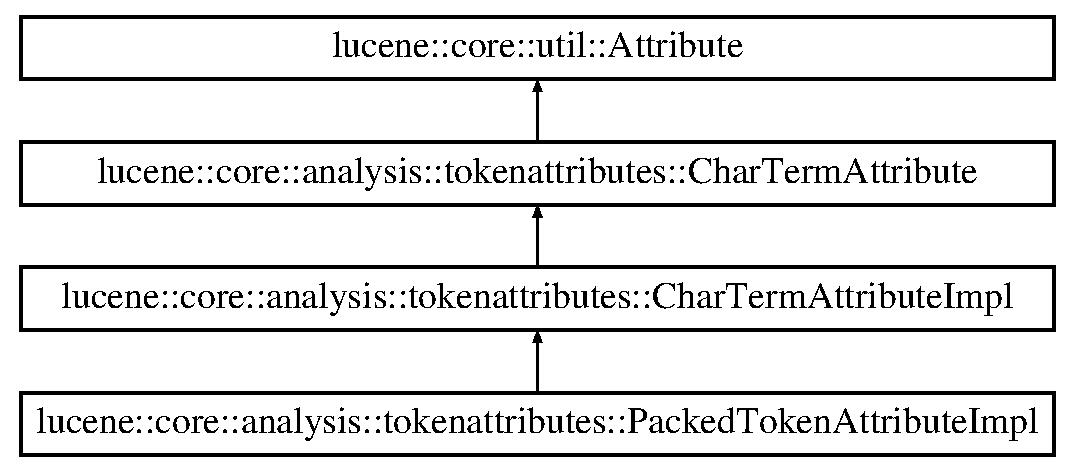
\includegraphics[height=4.000000cm]{classlucene_1_1core_1_1analysis_1_1tokenattributes_1_1CharTermAttribute}
\end{center}
\end{figure}
\subsection*{Public Member Functions}
\begin{DoxyCompactItemize}
\item 
virtual \mbox{\hyperlink{classlucene_1_1core_1_1analysis_1_1tokenattributes_1_1CharTermAttribute_a44922cdddac47f06e60c0e69c78599ad}{$\sim$\+Char\+Term\+Attribute}} ()
\item 
virtual void \mbox{\hyperlink{classlucene_1_1core_1_1analysis_1_1tokenattributes_1_1CharTermAttribute_ae03cbeb05b5b1e7c50f407e0025d41da}{Copy\+Buffer}} (\mbox{\hyperlink{ZlibCrc32_8h_a2c212835823e3c54a8ab6d95c652660e}{const}} char $\ast$buffer, \mbox{\hyperlink{ZlibCrc32_8h_a2c212835823e3c54a8ab6d95c652660e}{const}} uint32\+\_\+t offset, \mbox{\hyperlink{ZlibCrc32_8h_a2c212835823e3c54a8ab6d95c652660e}{const}} uint32\+\_\+t length)=0
\item 
virtual char $\ast$ \mbox{\hyperlink{classlucene_1_1core_1_1analysis_1_1tokenattributes_1_1CharTermAttribute_abc9fbea4b68b4cdbb1d120970c71d38e}{Buffer}} () \mbox{\hyperlink{ZlibCrc32_8h_a2c212835823e3c54a8ab6d95c652660e}{const}} =0
\item 
virtual char $\ast$ \mbox{\hyperlink{classlucene_1_1core_1_1analysis_1_1tokenattributes_1_1CharTermAttribute_ada68e9c9011b5ac61e9a34caf63aba6d}{Resize\+Buffer}} (\mbox{\hyperlink{ZlibCrc32_8h_a2c212835823e3c54a8ab6d95c652660e}{const}} uint32\+\_\+t new\+\_\+size)=0
\item 
virtual uint32\+\_\+t \mbox{\hyperlink{classlucene_1_1core_1_1analysis_1_1tokenattributes_1_1CharTermAttribute_a1e81ad4ff6bc6141f5a6e103cdf7f36d}{Length}} () \mbox{\hyperlink{ZlibCrc32_8h_a2c212835823e3c54a8ab6d95c652660e}{const}} =0
\item 
virtual char \& \mbox{\hyperlink{classlucene_1_1core_1_1analysis_1_1tokenattributes_1_1CharTermAttribute_af6a554c50515313093c1ac61c3bddbe7}{operator\mbox{[}$\,$\mbox{]}}} (\mbox{\hyperlink{ZlibCrc32_8h_a2c212835823e3c54a8ab6d95c652660e}{const}} uint32\+\_\+t idx)=0
\item 
virtual std\+::string \mbox{\hyperlink{classlucene_1_1core_1_1analysis_1_1tokenattributes_1_1CharTermAttribute_af97534d3a549afbbddd5f64b97efc5a4}{Sub\+Sequence}} (\mbox{\hyperlink{ZlibCrc32_8h_a2c212835823e3c54a8ab6d95c652660e}{const}} uint32\+\_\+t start, \mbox{\hyperlink{ZlibCrc32_8h_a2c212835823e3c54a8ab6d95c652660e}{const}} uint32\+\_\+t end)=0
\item 
virtual \mbox{\hyperlink{classlucene_1_1core_1_1analysis_1_1tokenattributes_1_1CharTermAttribute}{Char\+Term\+Attribute}} \& \mbox{\hyperlink{classlucene_1_1core_1_1analysis_1_1tokenattributes_1_1CharTermAttribute_a8186262029561e196e991fc543cd9953}{Set\+Length}} (\mbox{\hyperlink{ZlibCrc32_8h_a2c212835823e3c54a8ab6d95c652660e}{const}} uint32\+\_\+t length)=0
\item 
virtual \mbox{\hyperlink{classlucene_1_1core_1_1analysis_1_1tokenattributes_1_1CharTermAttribute}{Char\+Term\+Attribute}} \& \mbox{\hyperlink{classlucene_1_1core_1_1analysis_1_1tokenattributes_1_1CharTermAttribute_ac14e6e064418d1d56b0f33724dcfe8b0}{Set\+Empty}} ()=0
\item 
virtual \mbox{\hyperlink{classlucene_1_1core_1_1analysis_1_1tokenattributes_1_1CharTermAttribute}{Char\+Term\+Attribute}} \& \mbox{\hyperlink{classlucene_1_1core_1_1analysis_1_1tokenattributes_1_1CharTermAttribute_a721493e2513c3cbb5818cab4ec36e277}{Append}} (\mbox{\hyperlink{ZlibCrc32_8h_a2c212835823e3c54a8ab6d95c652660e}{const}} std\+::string \&csq)=0
\item 
virtual \mbox{\hyperlink{classlucene_1_1core_1_1analysis_1_1tokenattributes_1_1CharTermAttribute}{Char\+Term\+Attribute}} \& \mbox{\hyperlink{classlucene_1_1core_1_1analysis_1_1tokenattributes_1_1CharTermAttribute_a1fc0d3eaff550a10e8fc17a5e7bb98bc}{Append}} (\mbox{\hyperlink{ZlibCrc32_8h_a2c212835823e3c54a8ab6d95c652660e}{const}} std\+::string \&csq, \mbox{\hyperlink{ZlibCrc32_8h_a2c212835823e3c54a8ab6d95c652660e}{const}} uint32\+\_\+t start, \mbox{\hyperlink{ZlibCrc32_8h_a2c212835823e3c54a8ab6d95c652660e}{const}} uint32\+\_\+t end)=0
\item 
virtual \mbox{\hyperlink{classlucene_1_1core_1_1analysis_1_1tokenattributes_1_1CharTermAttribute}{Char\+Term\+Attribute}} \& \mbox{\hyperlink{classlucene_1_1core_1_1analysis_1_1tokenattributes_1_1CharTermAttribute_a069f61e1cb30895a205e615c1d154148}{Append}} (\mbox{\hyperlink{ZlibCrc32_8h_a2c212835823e3c54a8ab6d95c652660e}{const}} char c)=0
\item 
virtual \mbox{\hyperlink{classlucene_1_1core_1_1analysis_1_1tokenattributes_1_1CharTermAttribute}{Char\+Term\+Attribute}} \& \mbox{\hyperlink{classlucene_1_1core_1_1analysis_1_1tokenattributes_1_1CharTermAttribute_ad8624358a4798446a14fbf35991c43ad}{Append}} (\mbox{\hyperlink{ZlibCrc32_8h_a2c212835823e3c54a8ab6d95c652660e}{const}} \mbox{\hyperlink{classlucene_1_1core_1_1analysis_1_1tokenattributes_1_1CharTermAttribute}{Char\+Term\+Attribute}} \&term\+\_\+att)=0
\end{DoxyCompactItemize}
\subsection*{Additional Inherited Members}


\subsection{Constructor \& Destructor Documentation}
\mbox{\Hypertarget{classlucene_1_1core_1_1analysis_1_1tokenattributes_1_1CharTermAttribute_a44922cdddac47f06e60c0e69c78599ad}\label{classlucene_1_1core_1_1analysis_1_1tokenattributes_1_1CharTermAttribute_a44922cdddac47f06e60c0e69c78599ad}} 
\index{lucene\+::core\+::analysis\+::tokenattributes\+::\+Char\+Term\+Attribute@{lucene\+::core\+::analysis\+::tokenattributes\+::\+Char\+Term\+Attribute}!````~Char\+Term\+Attribute@{$\sim$\+Char\+Term\+Attribute}}
\index{````~Char\+Term\+Attribute@{$\sim$\+Char\+Term\+Attribute}!lucene\+::core\+::analysis\+::tokenattributes\+::\+Char\+Term\+Attribute@{lucene\+::core\+::analysis\+::tokenattributes\+::\+Char\+Term\+Attribute}}
\subsubsection{\texorpdfstring{$\sim$\+Char\+Term\+Attribute()}{~CharTermAttribute()}}
{\footnotesize\ttfamily virtual lucene\+::core\+::analysis\+::tokenattributes\+::\+Char\+Term\+Attribute\+::$\sim$\+Char\+Term\+Attribute (\begin{DoxyParamCaption}{ }\end{DoxyParamCaption})\hspace{0.3cm}{\ttfamily [inline]}, {\ttfamily [virtual]}}



\subsection{Member Function Documentation}
\mbox{\Hypertarget{classlucene_1_1core_1_1analysis_1_1tokenattributes_1_1CharTermAttribute_a721493e2513c3cbb5818cab4ec36e277}\label{classlucene_1_1core_1_1analysis_1_1tokenattributes_1_1CharTermAttribute_a721493e2513c3cbb5818cab4ec36e277}} 
\index{lucene\+::core\+::analysis\+::tokenattributes\+::\+Char\+Term\+Attribute@{lucene\+::core\+::analysis\+::tokenattributes\+::\+Char\+Term\+Attribute}!Append@{Append}}
\index{Append@{Append}!lucene\+::core\+::analysis\+::tokenattributes\+::\+Char\+Term\+Attribute@{lucene\+::core\+::analysis\+::tokenattributes\+::\+Char\+Term\+Attribute}}
\subsubsection{\texorpdfstring{Append()}{Append()}\hspace{0.1cm}{\footnotesize\ttfamily [1/4]}}
{\footnotesize\ttfamily virtual \mbox{\hyperlink{classlucene_1_1core_1_1analysis_1_1tokenattributes_1_1CharTermAttribute}{Char\+Term\+Attribute}}\& lucene\+::core\+::analysis\+::tokenattributes\+::\+Char\+Term\+Attribute\+::\+Append (\begin{DoxyParamCaption}\item[{\mbox{\hyperlink{ZlibCrc32_8h_a2c212835823e3c54a8ab6d95c652660e}{const}} std\+::string \&}]{csq }\end{DoxyParamCaption})\hspace{0.3cm}{\ttfamily [pure virtual]}}



Implemented in \mbox{\hyperlink{classlucene_1_1core_1_1analysis_1_1tokenattributes_1_1CharTermAttributeImpl_aaf6bf26fa572599e284845f67b444900}{lucene\+::core\+::analysis\+::tokenattributes\+::\+Char\+Term\+Attribute\+Impl}}.

\mbox{\Hypertarget{classlucene_1_1core_1_1analysis_1_1tokenattributes_1_1CharTermAttribute_a1fc0d3eaff550a10e8fc17a5e7bb98bc}\label{classlucene_1_1core_1_1analysis_1_1tokenattributes_1_1CharTermAttribute_a1fc0d3eaff550a10e8fc17a5e7bb98bc}} 
\index{lucene\+::core\+::analysis\+::tokenattributes\+::\+Char\+Term\+Attribute@{lucene\+::core\+::analysis\+::tokenattributes\+::\+Char\+Term\+Attribute}!Append@{Append}}
\index{Append@{Append}!lucene\+::core\+::analysis\+::tokenattributes\+::\+Char\+Term\+Attribute@{lucene\+::core\+::analysis\+::tokenattributes\+::\+Char\+Term\+Attribute}}
\subsubsection{\texorpdfstring{Append()}{Append()}\hspace{0.1cm}{\footnotesize\ttfamily [2/4]}}
{\footnotesize\ttfamily virtual \mbox{\hyperlink{classlucene_1_1core_1_1analysis_1_1tokenattributes_1_1CharTermAttribute}{Char\+Term\+Attribute}}\& lucene\+::core\+::analysis\+::tokenattributes\+::\+Char\+Term\+Attribute\+::\+Append (\begin{DoxyParamCaption}\item[{\mbox{\hyperlink{ZlibCrc32_8h_a2c212835823e3c54a8ab6d95c652660e}{const}} std\+::string \&}]{csq,  }\item[{\mbox{\hyperlink{ZlibCrc32_8h_a2c212835823e3c54a8ab6d95c652660e}{const}} uint32\+\_\+t}]{start,  }\item[{\mbox{\hyperlink{ZlibCrc32_8h_a2c212835823e3c54a8ab6d95c652660e}{const}} uint32\+\_\+t}]{end }\end{DoxyParamCaption})\hspace{0.3cm}{\ttfamily [pure virtual]}}



Implemented in \mbox{\hyperlink{classlucene_1_1core_1_1analysis_1_1tokenattributes_1_1CharTermAttributeImpl_a5d2f89510d37dc11bbf22a77ac6bff83}{lucene\+::core\+::analysis\+::tokenattributes\+::\+Char\+Term\+Attribute\+Impl}}.

\mbox{\Hypertarget{classlucene_1_1core_1_1analysis_1_1tokenattributes_1_1CharTermAttribute_a069f61e1cb30895a205e615c1d154148}\label{classlucene_1_1core_1_1analysis_1_1tokenattributes_1_1CharTermAttribute_a069f61e1cb30895a205e615c1d154148}} 
\index{lucene\+::core\+::analysis\+::tokenattributes\+::\+Char\+Term\+Attribute@{lucene\+::core\+::analysis\+::tokenattributes\+::\+Char\+Term\+Attribute}!Append@{Append}}
\index{Append@{Append}!lucene\+::core\+::analysis\+::tokenattributes\+::\+Char\+Term\+Attribute@{lucene\+::core\+::analysis\+::tokenattributes\+::\+Char\+Term\+Attribute}}
\subsubsection{\texorpdfstring{Append()}{Append()}\hspace{0.1cm}{\footnotesize\ttfamily [3/4]}}
{\footnotesize\ttfamily virtual \mbox{\hyperlink{classlucene_1_1core_1_1analysis_1_1tokenattributes_1_1CharTermAttribute}{Char\+Term\+Attribute}}\& lucene\+::core\+::analysis\+::tokenattributes\+::\+Char\+Term\+Attribute\+::\+Append (\begin{DoxyParamCaption}\item[{\mbox{\hyperlink{ZlibCrc32_8h_a2c212835823e3c54a8ab6d95c652660e}{const}} char}]{c }\end{DoxyParamCaption})\hspace{0.3cm}{\ttfamily [pure virtual]}}



Implemented in \mbox{\hyperlink{classlucene_1_1core_1_1analysis_1_1tokenattributes_1_1CharTermAttributeImpl_a1f8dccf1ecc42396f7f97b6a1972325f}{lucene\+::core\+::analysis\+::tokenattributes\+::\+Char\+Term\+Attribute\+Impl}}.

\mbox{\Hypertarget{classlucene_1_1core_1_1analysis_1_1tokenattributes_1_1CharTermAttribute_ad8624358a4798446a14fbf35991c43ad}\label{classlucene_1_1core_1_1analysis_1_1tokenattributes_1_1CharTermAttribute_ad8624358a4798446a14fbf35991c43ad}} 
\index{lucene\+::core\+::analysis\+::tokenattributes\+::\+Char\+Term\+Attribute@{lucene\+::core\+::analysis\+::tokenattributes\+::\+Char\+Term\+Attribute}!Append@{Append}}
\index{Append@{Append}!lucene\+::core\+::analysis\+::tokenattributes\+::\+Char\+Term\+Attribute@{lucene\+::core\+::analysis\+::tokenattributes\+::\+Char\+Term\+Attribute}}
\subsubsection{\texorpdfstring{Append()}{Append()}\hspace{0.1cm}{\footnotesize\ttfamily [4/4]}}
{\footnotesize\ttfamily virtual \mbox{\hyperlink{classlucene_1_1core_1_1analysis_1_1tokenattributes_1_1CharTermAttribute}{Char\+Term\+Attribute}}\& lucene\+::core\+::analysis\+::tokenattributes\+::\+Char\+Term\+Attribute\+::\+Append (\begin{DoxyParamCaption}\item[{\mbox{\hyperlink{ZlibCrc32_8h_a2c212835823e3c54a8ab6d95c652660e}{const}} \mbox{\hyperlink{classlucene_1_1core_1_1analysis_1_1tokenattributes_1_1CharTermAttribute}{Char\+Term\+Attribute}} \&}]{term\+\_\+att }\end{DoxyParamCaption})\hspace{0.3cm}{\ttfamily [pure virtual]}}



Implemented in \mbox{\hyperlink{classlucene_1_1core_1_1analysis_1_1tokenattributes_1_1CharTermAttributeImpl_ab8c8f791a3a504d86b3578a6f43810d1}{lucene\+::core\+::analysis\+::tokenattributes\+::\+Char\+Term\+Attribute\+Impl}}.

\mbox{\Hypertarget{classlucene_1_1core_1_1analysis_1_1tokenattributes_1_1CharTermAttribute_abc9fbea4b68b4cdbb1d120970c71d38e}\label{classlucene_1_1core_1_1analysis_1_1tokenattributes_1_1CharTermAttribute_abc9fbea4b68b4cdbb1d120970c71d38e}} 
\index{lucene\+::core\+::analysis\+::tokenattributes\+::\+Char\+Term\+Attribute@{lucene\+::core\+::analysis\+::tokenattributes\+::\+Char\+Term\+Attribute}!Buffer@{Buffer}}
\index{Buffer@{Buffer}!lucene\+::core\+::analysis\+::tokenattributes\+::\+Char\+Term\+Attribute@{lucene\+::core\+::analysis\+::tokenattributes\+::\+Char\+Term\+Attribute}}
\subsubsection{\texorpdfstring{Buffer()}{Buffer()}}
{\footnotesize\ttfamily virtual char$\ast$ lucene\+::core\+::analysis\+::tokenattributes\+::\+Char\+Term\+Attribute\+::\+Buffer (\begin{DoxyParamCaption}{ }\end{DoxyParamCaption}) const\hspace{0.3cm}{\ttfamily [pure virtual]}}



Implemented in \mbox{\hyperlink{classlucene_1_1core_1_1analysis_1_1tokenattributes_1_1CharTermAttributeImpl_af6663b6b4481ee51bd166f5c3123f9f8}{lucene\+::core\+::analysis\+::tokenattributes\+::\+Char\+Term\+Attribute\+Impl}}.

\mbox{\Hypertarget{classlucene_1_1core_1_1analysis_1_1tokenattributes_1_1CharTermAttribute_ae03cbeb05b5b1e7c50f407e0025d41da}\label{classlucene_1_1core_1_1analysis_1_1tokenattributes_1_1CharTermAttribute_ae03cbeb05b5b1e7c50f407e0025d41da}} 
\index{lucene\+::core\+::analysis\+::tokenattributes\+::\+Char\+Term\+Attribute@{lucene\+::core\+::analysis\+::tokenattributes\+::\+Char\+Term\+Attribute}!Copy\+Buffer@{Copy\+Buffer}}
\index{Copy\+Buffer@{Copy\+Buffer}!lucene\+::core\+::analysis\+::tokenattributes\+::\+Char\+Term\+Attribute@{lucene\+::core\+::analysis\+::tokenattributes\+::\+Char\+Term\+Attribute}}
\subsubsection{\texorpdfstring{Copy\+Buffer()}{CopyBuffer()}}
{\footnotesize\ttfamily virtual void lucene\+::core\+::analysis\+::tokenattributes\+::\+Char\+Term\+Attribute\+::\+Copy\+Buffer (\begin{DoxyParamCaption}\item[{\mbox{\hyperlink{ZlibCrc32_8h_a2c212835823e3c54a8ab6d95c652660e}{const}} char $\ast$}]{buffer,  }\item[{\mbox{\hyperlink{ZlibCrc32_8h_a2c212835823e3c54a8ab6d95c652660e}{const}} uint32\+\_\+t}]{offset,  }\item[{\mbox{\hyperlink{ZlibCrc32_8h_a2c212835823e3c54a8ab6d95c652660e}{const}} uint32\+\_\+t}]{length }\end{DoxyParamCaption})\hspace{0.3cm}{\ttfamily [pure virtual]}}



Implemented in \mbox{\hyperlink{classlucene_1_1core_1_1analysis_1_1tokenattributes_1_1CharTermAttributeImpl_aacb3a44d6999a381dc9217616ba91317}{lucene\+::core\+::analysis\+::tokenattributes\+::\+Char\+Term\+Attribute\+Impl}}.

\mbox{\Hypertarget{classlucene_1_1core_1_1analysis_1_1tokenattributes_1_1CharTermAttribute_a1e81ad4ff6bc6141f5a6e103cdf7f36d}\label{classlucene_1_1core_1_1analysis_1_1tokenattributes_1_1CharTermAttribute_a1e81ad4ff6bc6141f5a6e103cdf7f36d}} 
\index{lucene\+::core\+::analysis\+::tokenattributes\+::\+Char\+Term\+Attribute@{lucene\+::core\+::analysis\+::tokenattributes\+::\+Char\+Term\+Attribute}!Length@{Length}}
\index{Length@{Length}!lucene\+::core\+::analysis\+::tokenattributes\+::\+Char\+Term\+Attribute@{lucene\+::core\+::analysis\+::tokenattributes\+::\+Char\+Term\+Attribute}}
\subsubsection{\texorpdfstring{Length()}{Length()}}
{\footnotesize\ttfamily virtual uint32\+\_\+t lucene\+::core\+::analysis\+::tokenattributes\+::\+Char\+Term\+Attribute\+::\+Length (\begin{DoxyParamCaption}{ }\end{DoxyParamCaption}) const\hspace{0.3cm}{\ttfamily [pure virtual]}}



Implemented in \mbox{\hyperlink{classlucene_1_1core_1_1analysis_1_1tokenattributes_1_1CharTermAttributeImpl_a20085f30b788448e61de1f5635cd95f0}{lucene\+::core\+::analysis\+::tokenattributes\+::\+Char\+Term\+Attribute\+Impl}}.

\mbox{\Hypertarget{classlucene_1_1core_1_1analysis_1_1tokenattributes_1_1CharTermAttribute_af6a554c50515313093c1ac61c3bddbe7}\label{classlucene_1_1core_1_1analysis_1_1tokenattributes_1_1CharTermAttribute_af6a554c50515313093c1ac61c3bddbe7}} 
\index{lucene\+::core\+::analysis\+::tokenattributes\+::\+Char\+Term\+Attribute@{lucene\+::core\+::analysis\+::tokenattributes\+::\+Char\+Term\+Attribute}!operator\mbox{[}\mbox{]}@{operator[]}}
\index{operator\mbox{[}\mbox{]}@{operator[]}!lucene\+::core\+::analysis\+::tokenattributes\+::\+Char\+Term\+Attribute@{lucene\+::core\+::analysis\+::tokenattributes\+::\+Char\+Term\+Attribute}}
\subsubsection{\texorpdfstring{operator[]()}{operator[]()}}
{\footnotesize\ttfamily virtual char\& lucene\+::core\+::analysis\+::tokenattributes\+::\+Char\+Term\+Attribute\+::operator\mbox{[}$\,$\mbox{]} (\begin{DoxyParamCaption}\item[{\mbox{\hyperlink{ZlibCrc32_8h_a2c212835823e3c54a8ab6d95c652660e}{const}} uint32\+\_\+t}]{idx }\end{DoxyParamCaption})\hspace{0.3cm}{\ttfamily [pure virtual]}}



Implemented in \mbox{\hyperlink{classlucene_1_1core_1_1analysis_1_1tokenattributes_1_1CharTermAttributeImpl_a65259a0e94791f009d7109f7bbd7d74e}{lucene\+::core\+::analysis\+::tokenattributes\+::\+Char\+Term\+Attribute\+Impl}}.

\mbox{\Hypertarget{classlucene_1_1core_1_1analysis_1_1tokenattributes_1_1CharTermAttribute_ada68e9c9011b5ac61e9a34caf63aba6d}\label{classlucene_1_1core_1_1analysis_1_1tokenattributes_1_1CharTermAttribute_ada68e9c9011b5ac61e9a34caf63aba6d}} 
\index{lucene\+::core\+::analysis\+::tokenattributes\+::\+Char\+Term\+Attribute@{lucene\+::core\+::analysis\+::tokenattributes\+::\+Char\+Term\+Attribute}!Resize\+Buffer@{Resize\+Buffer}}
\index{Resize\+Buffer@{Resize\+Buffer}!lucene\+::core\+::analysis\+::tokenattributes\+::\+Char\+Term\+Attribute@{lucene\+::core\+::analysis\+::tokenattributes\+::\+Char\+Term\+Attribute}}
\subsubsection{\texorpdfstring{Resize\+Buffer()}{ResizeBuffer()}}
{\footnotesize\ttfamily virtual char$\ast$ lucene\+::core\+::analysis\+::tokenattributes\+::\+Char\+Term\+Attribute\+::\+Resize\+Buffer (\begin{DoxyParamCaption}\item[{\mbox{\hyperlink{ZlibCrc32_8h_a2c212835823e3c54a8ab6d95c652660e}{const}} uint32\+\_\+t}]{new\+\_\+size }\end{DoxyParamCaption})\hspace{0.3cm}{\ttfamily [pure virtual]}}



Implemented in \mbox{\hyperlink{classlucene_1_1core_1_1analysis_1_1tokenattributes_1_1CharTermAttributeImpl_abc195e8927e23632d34d4c081ede76b4}{lucene\+::core\+::analysis\+::tokenattributes\+::\+Char\+Term\+Attribute\+Impl}}.

\mbox{\Hypertarget{classlucene_1_1core_1_1analysis_1_1tokenattributes_1_1CharTermAttribute_ac14e6e064418d1d56b0f33724dcfe8b0}\label{classlucene_1_1core_1_1analysis_1_1tokenattributes_1_1CharTermAttribute_ac14e6e064418d1d56b0f33724dcfe8b0}} 
\index{lucene\+::core\+::analysis\+::tokenattributes\+::\+Char\+Term\+Attribute@{lucene\+::core\+::analysis\+::tokenattributes\+::\+Char\+Term\+Attribute}!Set\+Empty@{Set\+Empty}}
\index{Set\+Empty@{Set\+Empty}!lucene\+::core\+::analysis\+::tokenattributes\+::\+Char\+Term\+Attribute@{lucene\+::core\+::analysis\+::tokenattributes\+::\+Char\+Term\+Attribute}}
\subsubsection{\texorpdfstring{Set\+Empty()}{SetEmpty()}}
{\footnotesize\ttfamily virtual \mbox{\hyperlink{classlucene_1_1core_1_1analysis_1_1tokenattributes_1_1CharTermAttribute}{Char\+Term\+Attribute}}\& lucene\+::core\+::analysis\+::tokenattributes\+::\+Char\+Term\+Attribute\+::\+Set\+Empty (\begin{DoxyParamCaption}{ }\end{DoxyParamCaption})\hspace{0.3cm}{\ttfamily [pure virtual]}}



Implemented in \mbox{\hyperlink{classlucene_1_1core_1_1analysis_1_1tokenattributes_1_1CharTermAttributeImpl_a328d66d5bfd40a9bcd91ffe59933bc15}{lucene\+::core\+::analysis\+::tokenattributes\+::\+Char\+Term\+Attribute\+Impl}}.

\mbox{\Hypertarget{classlucene_1_1core_1_1analysis_1_1tokenattributes_1_1CharTermAttribute_a8186262029561e196e991fc543cd9953}\label{classlucene_1_1core_1_1analysis_1_1tokenattributes_1_1CharTermAttribute_a8186262029561e196e991fc543cd9953}} 
\index{lucene\+::core\+::analysis\+::tokenattributes\+::\+Char\+Term\+Attribute@{lucene\+::core\+::analysis\+::tokenattributes\+::\+Char\+Term\+Attribute}!Set\+Length@{Set\+Length}}
\index{Set\+Length@{Set\+Length}!lucene\+::core\+::analysis\+::tokenattributes\+::\+Char\+Term\+Attribute@{lucene\+::core\+::analysis\+::tokenattributes\+::\+Char\+Term\+Attribute}}
\subsubsection{\texorpdfstring{Set\+Length()}{SetLength()}}
{\footnotesize\ttfamily virtual \mbox{\hyperlink{classlucene_1_1core_1_1analysis_1_1tokenattributes_1_1CharTermAttribute}{Char\+Term\+Attribute}}\& lucene\+::core\+::analysis\+::tokenattributes\+::\+Char\+Term\+Attribute\+::\+Set\+Length (\begin{DoxyParamCaption}\item[{\mbox{\hyperlink{ZlibCrc32_8h_a2c212835823e3c54a8ab6d95c652660e}{const}} uint32\+\_\+t}]{length }\end{DoxyParamCaption})\hspace{0.3cm}{\ttfamily [pure virtual]}}



Implemented in \mbox{\hyperlink{classlucene_1_1core_1_1analysis_1_1tokenattributes_1_1CharTermAttributeImpl_a752c93bfaa290094349858306468c9a9}{lucene\+::core\+::analysis\+::tokenattributes\+::\+Char\+Term\+Attribute\+Impl}}.

\mbox{\Hypertarget{classlucene_1_1core_1_1analysis_1_1tokenattributes_1_1CharTermAttribute_af97534d3a549afbbddd5f64b97efc5a4}\label{classlucene_1_1core_1_1analysis_1_1tokenattributes_1_1CharTermAttribute_af97534d3a549afbbddd5f64b97efc5a4}} 
\index{lucene\+::core\+::analysis\+::tokenattributes\+::\+Char\+Term\+Attribute@{lucene\+::core\+::analysis\+::tokenattributes\+::\+Char\+Term\+Attribute}!Sub\+Sequence@{Sub\+Sequence}}
\index{Sub\+Sequence@{Sub\+Sequence}!lucene\+::core\+::analysis\+::tokenattributes\+::\+Char\+Term\+Attribute@{lucene\+::core\+::analysis\+::tokenattributes\+::\+Char\+Term\+Attribute}}
\subsubsection{\texorpdfstring{Sub\+Sequence()}{SubSequence()}}
{\footnotesize\ttfamily virtual std\+::string lucene\+::core\+::analysis\+::tokenattributes\+::\+Char\+Term\+Attribute\+::\+Sub\+Sequence (\begin{DoxyParamCaption}\item[{\mbox{\hyperlink{ZlibCrc32_8h_a2c212835823e3c54a8ab6d95c652660e}{const}} uint32\+\_\+t}]{start,  }\item[{\mbox{\hyperlink{ZlibCrc32_8h_a2c212835823e3c54a8ab6d95c652660e}{const}} uint32\+\_\+t}]{end }\end{DoxyParamCaption})\hspace{0.3cm}{\ttfamily [pure virtual]}}



Implemented in \mbox{\hyperlink{classlucene_1_1core_1_1analysis_1_1tokenattributes_1_1CharTermAttributeImpl_a286d2dd38ce24fb0da4c077e8f06bb25}{lucene\+::core\+::analysis\+::tokenattributes\+::\+Char\+Term\+Attribute\+Impl}}.



The documentation for this class was generated from the following file\+:\begin{DoxyCompactItemize}
\item 
Analysis/\mbox{\hyperlink{Analysis_2Attribute_8h}{Attribute.\+h}}\end{DoxyCompactItemize}

\hypertarget{classlucene_1_1core_1_1analysis_1_1tokenattributes_1_1CharTermAttributeImpl}{}\section{lucene\+:\+:core\+:\+:analysis\+:\+:tokenattributes\+:\+:Char\+Term\+Attribute\+Impl Class Reference}
\label{classlucene_1_1core_1_1analysis_1_1tokenattributes_1_1CharTermAttributeImpl}\index{lucene\+::core\+::analysis\+::tokenattributes\+::\+Char\+Term\+Attribute\+Impl@{lucene\+::core\+::analysis\+::tokenattributes\+::\+Char\+Term\+Attribute\+Impl}}


{\ttfamily \#include $<$Attribute\+Impl.\+h$>$}

Inheritance diagram for lucene\+:\+:core\+:\+:analysis\+:\+:tokenattributes\+:\+:Char\+Term\+Attribute\+Impl\+:\begin{figure}[H]
\begin{center}
\leavevmode
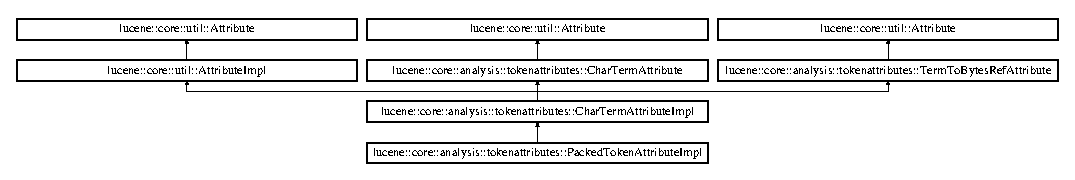
\includegraphics[height=1.964912cm]{classlucene_1_1core_1_1analysis_1_1tokenattributes_1_1CharTermAttributeImpl}
\end{center}
\end{figure}
\subsection*{Public Member Functions}
\begin{DoxyCompactItemize}
\item 
\mbox{\hyperlink{classlucene_1_1core_1_1analysis_1_1tokenattributes_1_1CharTermAttributeImpl_a3f0f1dfd6edd1686f46fa84b95b17959}{Char\+Term\+Attribute\+Impl}} ()
\item 
\mbox{\hyperlink{classlucene_1_1core_1_1analysis_1_1tokenattributes_1_1CharTermAttributeImpl_af846d32513f9e11a0b7443ea0ba41487}{Char\+Term\+Attribute\+Impl}} (\mbox{\hyperlink{ZlibCrc32_8h_a2c212835823e3c54a8ab6d95c652660e}{const}} \mbox{\hyperlink{classlucene_1_1core_1_1analysis_1_1tokenattributes_1_1CharTermAttributeImpl}{Char\+Term\+Attribute\+Impl}} \&other)
\item 
virtual \mbox{\hyperlink{classlucene_1_1core_1_1analysis_1_1tokenattributes_1_1CharTermAttributeImpl_aef0a9228f5cf3d4ad4c33d97f2a9a13b}{$\sim$\+Char\+Term\+Attribute\+Impl}} ()
\item 
\mbox{\hyperlink{classlucene_1_1core_1_1util_1_1BytesRef}{lucene\+::core\+::util\+::\+Bytes\+Ref}} \& \mbox{\hyperlink{classlucene_1_1core_1_1analysis_1_1tokenattributes_1_1CharTermAttributeImpl_aefef8491e2a12493480fe19dd6d61ca7}{Get\+Bytes\+Ref}} () override
\item 
void \mbox{\hyperlink{classlucene_1_1core_1_1analysis_1_1tokenattributes_1_1CharTermAttributeImpl_a4e0b1a5a06996822798414f3a41af6e6}{Clear}} () override
\item 
void \mbox{\hyperlink{classlucene_1_1core_1_1analysis_1_1tokenattributes_1_1CharTermAttributeImpl_aacb3a44d6999a381dc9217616ba91317}{Copy\+Buffer}} (\mbox{\hyperlink{ZlibCrc32_8h_a2c212835823e3c54a8ab6d95c652660e}{const}} char $\ast$buffer, \mbox{\hyperlink{ZlibCrc32_8h_a2c212835823e3c54a8ab6d95c652660e}{const}} uint32\+\_\+t offset, \mbox{\hyperlink{ZlibCrc32_8h_a2c212835823e3c54a8ab6d95c652660e}{const}} uint32\+\_\+t length) override
\item 
char $\ast$ \mbox{\hyperlink{classlucene_1_1core_1_1analysis_1_1tokenattributes_1_1CharTermAttributeImpl_af6663b6b4481ee51bd166f5c3123f9f8}{Buffer}} () \mbox{\hyperlink{ZlibCrc32_8h_a2c212835823e3c54a8ab6d95c652660e}{const}} override
\item 
char $\ast$ \mbox{\hyperlink{classlucene_1_1core_1_1analysis_1_1tokenattributes_1_1CharTermAttributeImpl_abc195e8927e23632d34d4c081ede76b4}{Resize\+Buffer}} (\mbox{\hyperlink{ZlibCrc32_8h_a2c212835823e3c54a8ab6d95c652660e}{const}} uint32\+\_\+t new\+\_\+capacity) override
\item 
uint32\+\_\+t \mbox{\hyperlink{classlucene_1_1core_1_1analysis_1_1tokenattributes_1_1CharTermAttributeImpl_a20085f30b788448e61de1f5635cd95f0}{Length}} () \mbox{\hyperlink{ZlibCrc32_8h_a2c212835823e3c54a8ab6d95c652660e}{const}} override
\item 
std\+::string \mbox{\hyperlink{classlucene_1_1core_1_1analysis_1_1tokenattributes_1_1CharTermAttributeImpl_a286d2dd38ce24fb0da4c077e8f06bb25}{Sub\+Sequence}} (\mbox{\hyperlink{ZlibCrc32_8h_a2c212835823e3c54a8ab6d95c652660e}{const}} uint32\+\_\+t inclusive\+\_\+start, \mbox{\hyperlink{ZlibCrc32_8h_a2c212835823e3c54a8ab6d95c652660e}{const}} uint32\+\_\+t exclusive\+\_\+end) override
\item 
\mbox{\hyperlink{classlucene_1_1core_1_1analysis_1_1tokenattributes_1_1CharTermAttributeImpl}{Char\+Term\+Attribute\+Impl}} \& \mbox{\hyperlink{classlucene_1_1core_1_1analysis_1_1tokenattributes_1_1CharTermAttributeImpl_a752c93bfaa290094349858306468c9a9}{Set\+Length}} (\mbox{\hyperlink{ZlibCrc32_8h_a2c212835823e3c54a8ab6d95c652660e}{const}} uint32\+\_\+t length) override
\item 
\mbox{\hyperlink{classlucene_1_1core_1_1analysis_1_1tokenattributes_1_1CharTermAttributeImpl}{Char\+Term\+Attribute\+Impl}} \& \mbox{\hyperlink{classlucene_1_1core_1_1analysis_1_1tokenattributes_1_1CharTermAttributeImpl_a328d66d5bfd40a9bcd91ffe59933bc15}{Set\+Empty}} () override
\item 
\mbox{\hyperlink{classlucene_1_1core_1_1analysis_1_1tokenattributes_1_1CharTermAttribute}{Char\+Term\+Attribute}} \& \mbox{\hyperlink{classlucene_1_1core_1_1analysis_1_1tokenattributes_1_1CharTermAttributeImpl_aaf6bf26fa572599e284845f67b444900}{Append}} (\mbox{\hyperlink{ZlibCrc32_8h_a2c212835823e3c54a8ab6d95c652660e}{const}} std\+::string \&csq) override
\item 
\mbox{\hyperlink{classlucene_1_1core_1_1analysis_1_1tokenattributes_1_1CharTermAttribute}{Char\+Term\+Attribute}} \& \mbox{\hyperlink{classlucene_1_1core_1_1analysis_1_1tokenattributes_1_1CharTermAttributeImpl_a5d2f89510d37dc11bbf22a77ac6bff83}{Append}} (\mbox{\hyperlink{ZlibCrc32_8h_a2c212835823e3c54a8ab6d95c652660e}{const}} std\+::string \&csq, \mbox{\hyperlink{ZlibCrc32_8h_a2c212835823e3c54a8ab6d95c652660e}{const}} uint32\+\_\+t inclusive\+\_\+start, \mbox{\hyperlink{ZlibCrc32_8h_a2c212835823e3c54a8ab6d95c652660e}{const}} uint32\+\_\+t exclusive\+\_\+end) override
\item 
\mbox{\hyperlink{classlucene_1_1core_1_1analysis_1_1tokenattributes_1_1CharTermAttribute}{Char\+Term\+Attribute}} \& \mbox{\hyperlink{classlucene_1_1core_1_1analysis_1_1tokenattributes_1_1CharTermAttributeImpl_a1f8dccf1ecc42396f7f97b6a1972325f}{Append}} (\mbox{\hyperlink{ZlibCrc32_8h_a2c212835823e3c54a8ab6d95c652660e}{const}} char c) override
\item 
\mbox{\hyperlink{classlucene_1_1core_1_1analysis_1_1tokenattributes_1_1CharTermAttribute}{Char\+Term\+Attribute}} \& \mbox{\hyperlink{classlucene_1_1core_1_1analysis_1_1tokenattributes_1_1CharTermAttributeImpl_ab8c8f791a3a504d86b3578a6f43810d1}{Append}} (\mbox{\hyperlink{ZlibCrc32_8h_a2c212835823e3c54a8ab6d95c652660e}{const}} \mbox{\hyperlink{classlucene_1_1core_1_1analysis_1_1tokenattributes_1_1CharTermAttribute}{Char\+Term\+Attribute}} \&term\+\_\+att) override
\item 
void \mbox{\hyperlink{classlucene_1_1core_1_1analysis_1_1tokenattributes_1_1CharTermAttributeImpl_ae434068c40b8eab62af50e0e33a71bf4}{Reflect\+With}} (\mbox{\hyperlink{namespacelucene_1_1core_1_1util_a7dbb701adaed055f73fb95eec83da10a}{lucene\+::core\+::util\+::\+Attribute\+Reflector}} \&reflector) override
\item 
char \& \mbox{\hyperlink{classlucene_1_1core_1_1analysis_1_1tokenattributes_1_1CharTermAttributeImpl_a65259a0e94791f009d7109f7bbd7d74e}{operator\mbox{[}$\,$\mbox{]}}} (\mbox{\hyperlink{ZlibCrc32_8h_a2c212835823e3c54a8ab6d95c652660e}{const}} uint32\+\_\+t idx) override
\item 
bool \mbox{\hyperlink{classlucene_1_1core_1_1analysis_1_1tokenattributes_1_1CharTermAttributeImpl_a2d741886d3be18e04bcbc1fbccad62a1}{operator==}} (\mbox{\hyperlink{ZlibCrc32_8h_a2c212835823e3c54a8ab6d95c652660e}{const}} \mbox{\hyperlink{classlucene_1_1core_1_1analysis_1_1tokenattributes_1_1CharTermAttributeImpl}{Char\+Term\+Attribute\+Impl}} \&other) \mbox{\hyperlink{ZlibCrc32_8h_a2c212835823e3c54a8ab6d95c652660e}{const}}
\item 
std\+::vector$<$ std\+::type\+\_\+index $>$ \mbox{\hyperlink{classlucene_1_1core_1_1analysis_1_1tokenattributes_1_1CharTermAttributeImpl_a7d8986b373cd9c2dfb2de25dd12000fd}{Attributes}} () override
\item 
void \mbox{\hyperlink{classlucene_1_1core_1_1analysis_1_1tokenattributes_1_1CharTermAttributeImpl_ae37cc1fbce5614f5e60800d3f9f96d33}{Shallow\+Copy\+To}} (\mbox{\hyperlink{classlucene_1_1core_1_1util_1_1AttributeImpl}{lucene\+::core\+::util\+::\+Attribute\+Impl}} \&attr\+\_\+impl) override
\item 
\mbox{\hyperlink{classlucene_1_1core_1_1analysis_1_1tokenattributes_1_1CharTermAttributeImpl}{Char\+Term\+Attribute\+Impl}} \& \mbox{\hyperlink{classlucene_1_1core_1_1analysis_1_1tokenattributes_1_1CharTermAttributeImpl_ac49b714c3f8e438ddaa27dc1a2421144}{operator=}} (\mbox{\hyperlink{ZlibCrc32_8h_a2c212835823e3c54a8ab6d95c652660e}{const}} \mbox{\hyperlink{classlucene_1_1core_1_1util_1_1AttributeImpl}{lucene\+::core\+::util\+::\+Attribute\+Impl}} \&other)
\item 
\mbox{\hyperlink{classlucene_1_1core_1_1analysis_1_1tokenattributes_1_1CharTermAttributeImpl}{Char\+Term\+Attribute\+Impl}} \& \mbox{\hyperlink{classlucene_1_1core_1_1analysis_1_1tokenattributes_1_1CharTermAttributeImpl_a4a53d4368af86441243246af1722390f}{operator=}} (\mbox{\hyperlink{ZlibCrc32_8h_a2c212835823e3c54a8ab6d95c652660e}{const}} \mbox{\hyperlink{classlucene_1_1core_1_1analysis_1_1tokenattributes_1_1CharTermAttributeImpl}{Char\+Term\+Attribute\+Impl}} \&other)
\item 
\mbox{\hyperlink{classlucene_1_1core_1_1util_1_1AttributeImpl}{lucene\+::core\+::util\+::\+Attribute\+Impl}} $\ast$ \mbox{\hyperlink{classlucene_1_1core_1_1analysis_1_1tokenattributes_1_1CharTermAttributeImpl_a518bf3f405ddf676ee58fccb02ae3c23}{Clone}} () override
\end{DoxyCompactItemize}
\subsection*{Private Member Functions}
\begin{DoxyCompactItemize}
\item 
void \mbox{\hyperlink{classlucene_1_1core_1_1analysis_1_1tokenattributes_1_1CharTermAttributeImpl_a4e54d600b1368df46af61c9bdae71cc0}{Grow\+Term\+Buffer}} (\mbox{\hyperlink{ZlibCrc32_8h_a2c212835823e3c54a8ab6d95c652660e}{const}} uint32\+\_\+t new\+\_\+size)
\end{DoxyCompactItemize}
\subsection*{Private Attributes}
\begin{DoxyCompactItemize}
\item 
std\+::shared\+\_\+ptr$<$ char $>$ \mbox{\hyperlink{classlucene_1_1core_1_1analysis_1_1tokenattributes_1_1CharTermAttributeImpl_a9a4ece35b434c726c23ea3e1f0b46514}{term\+\_\+buffer}}
\item 
uint32\+\_\+t \mbox{\hyperlink{classlucene_1_1core_1_1analysis_1_1tokenattributes_1_1CharTermAttributeImpl_aa62aff36d884a989746a4de2cc12e921}{term\+\_\+capacity}}
\item 
uint32\+\_\+t \mbox{\hyperlink{classlucene_1_1core_1_1analysis_1_1tokenattributes_1_1CharTermAttributeImpl_a746eb5a710afd01df9c4170ea0e0ce3e}{term\+\_\+length}}
\item 
\mbox{\hyperlink{classlucene_1_1core_1_1util_1_1BytesRefBuilder}{lucene\+::core\+::util\+::\+Bytes\+Ref\+Builder}} \mbox{\hyperlink{classlucene_1_1core_1_1analysis_1_1tokenattributes_1_1CharTermAttributeImpl_a1599ca8cd8221d3970fdb6d3d5f763a9}{builder}}
\end{DoxyCompactItemize}
\subsection*{Static Private Attributes}
\begin{DoxyCompactItemize}
\item 
static \mbox{\hyperlink{ZlibCrc32_8h_a2c212835823e3c54a8ab6d95c652660e}{const}} uint32\+\_\+t \mbox{\hyperlink{classlucene_1_1core_1_1analysis_1_1tokenattributes_1_1CharTermAttributeImpl_af41df146fa133bcc320a7d281c559ae7}{C\+H\+A\+R\+\_\+\+T\+E\+R\+M\+\_\+\+A\+T\+T\+R\+I\+B\+U\+T\+E\+\_\+\+I\+M\+P\+L\+\_\+\+M\+I\+N\+\_\+\+B\+U\+F\+F\+E\+R\+\_\+\+S\+I\+ZE}} = 10
\end{DoxyCompactItemize}
\subsection*{Additional Inherited Members}


\subsection{Constructor \& Destructor Documentation}
\mbox{\Hypertarget{classlucene_1_1core_1_1analysis_1_1tokenattributes_1_1CharTermAttributeImpl_a3f0f1dfd6edd1686f46fa84b95b17959}\label{classlucene_1_1core_1_1analysis_1_1tokenattributes_1_1CharTermAttributeImpl_a3f0f1dfd6edd1686f46fa84b95b17959}} 
\index{lucene\+::core\+::analysis\+::tokenattributes\+::\+Char\+Term\+Attribute\+Impl@{lucene\+::core\+::analysis\+::tokenattributes\+::\+Char\+Term\+Attribute\+Impl}!Char\+Term\+Attribute\+Impl@{Char\+Term\+Attribute\+Impl}}
\index{Char\+Term\+Attribute\+Impl@{Char\+Term\+Attribute\+Impl}!lucene\+::core\+::analysis\+::tokenattributes\+::\+Char\+Term\+Attribute\+Impl@{lucene\+::core\+::analysis\+::tokenattributes\+::\+Char\+Term\+Attribute\+Impl}}
\subsubsection{\texorpdfstring{Char\+Term\+Attribute\+Impl()}{CharTermAttributeImpl()}\hspace{0.1cm}{\footnotesize\ttfamily [1/2]}}
{\footnotesize\ttfamily Char\+Term\+Attribute\+Impl\+::\+Char\+Term\+Attribute\+Impl (\begin{DoxyParamCaption}{ }\end{DoxyParamCaption})}

\mbox{\hyperlink{classlucene_1_1core_1_1analysis_1_1tokenattributes_1_1CharTermAttributeImpl}{Char\+Term\+Attribute\+Impl}} \mbox{\Hypertarget{classlucene_1_1core_1_1analysis_1_1tokenattributes_1_1CharTermAttributeImpl_af846d32513f9e11a0b7443ea0ba41487}\label{classlucene_1_1core_1_1analysis_1_1tokenattributes_1_1CharTermAttributeImpl_af846d32513f9e11a0b7443ea0ba41487}} 
\index{lucene\+::core\+::analysis\+::tokenattributes\+::\+Char\+Term\+Attribute\+Impl@{lucene\+::core\+::analysis\+::tokenattributes\+::\+Char\+Term\+Attribute\+Impl}!Char\+Term\+Attribute\+Impl@{Char\+Term\+Attribute\+Impl}}
\index{Char\+Term\+Attribute\+Impl@{Char\+Term\+Attribute\+Impl}!lucene\+::core\+::analysis\+::tokenattributes\+::\+Char\+Term\+Attribute\+Impl@{lucene\+::core\+::analysis\+::tokenattributes\+::\+Char\+Term\+Attribute\+Impl}}
\subsubsection{\texorpdfstring{Char\+Term\+Attribute\+Impl()}{CharTermAttributeImpl()}\hspace{0.1cm}{\footnotesize\ttfamily [2/2]}}
{\footnotesize\ttfamily Char\+Term\+Attribute\+Impl\+::\+Char\+Term\+Attribute\+Impl (\begin{DoxyParamCaption}\item[{\mbox{\hyperlink{ZlibCrc32_8h_a2c212835823e3c54a8ab6d95c652660e}{const}} \mbox{\hyperlink{classlucene_1_1core_1_1analysis_1_1tokenattributes_1_1CharTermAttributeImpl}{Char\+Term\+Attribute\+Impl}} \&}]{other }\end{DoxyParamCaption})}

\mbox{\Hypertarget{classlucene_1_1core_1_1analysis_1_1tokenattributes_1_1CharTermAttributeImpl_aef0a9228f5cf3d4ad4c33d97f2a9a13b}\label{classlucene_1_1core_1_1analysis_1_1tokenattributes_1_1CharTermAttributeImpl_aef0a9228f5cf3d4ad4c33d97f2a9a13b}} 
\index{lucene\+::core\+::analysis\+::tokenattributes\+::\+Char\+Term\+Attribute\+Impl@{lucene\+::core\+::analysis\+::tokenattributes\+::\+Char\+Term\+Attribute\+Impl}!````~Char\+Term\+Attribute\+Impl@{$\sim$\+Char\+Term\+Attribute\+Impl}}
\index{````~Char\+Term\+Attribute\+Impl@{$\sim$\+Char\+Term\+Attribute\+Impl}!lucene\+::core\+::analysis\+::tokenattributes\+::\+Char\+Term\+Attribute\+Impl@{lucene\+::core\+::analysis\+::tokenattributes\+::\+Char\+Term\+Attribute\+Impl}}
\subsubsection{\texorpdfstring{$\sim$\+Char\+Term\+Attribute\+Impl()}{~CharTermAttributeImpl()}}
{\footnotesize\ttfamily Char\+Term\+Attribute\+Impl\+::$\sim$\+Char\+Term\+Attribute\+Impl (\begin{DoxyParamCaption}{ }\end{DoxyParamCaption})\hspace{0.3cm}{\ttfamily [virtual]}}



\subsection{Member Function Documentation}
\mbox{\Hypertarget{classlucene_1_1core_1_1analysis_1_1tokenattributes_1_1CharTermAttributeImpl_aaf6bf26fa572599e284845f67b444900}\label{classlucene_1_1core_1_1analysis_1_1tokenattributes_1_1CharTermAttributeImpl_aaf6bf26fa572599e284845f67b444900}} 
\index{lucene\+::core\+::analysis\+::tokenattributes\+::\+Char\+Term\+Attribute\+Impl@{lucene\+::core\+::analysis\+::tokenattributes\+::\+Char\+Term\+Attribute\+Impl}!Append@{Append}}
\index{Append@{Append}!lucene\+::core\+::analysis\+::tokenattributes\+::\+Char\+Term\+Attribute\+Impl@{lucene\+::core\+::analysis\+::tokenattributes\+::\+Char\+Term\+Attribute\+Impl}}
\subsubsection{\texorpdfstring{Append()}{Append()}\hspace{0.1cm}{\footnotesize\ttfamily [1/4]}}
{\footnotesize\ttfamily \mbox{\hyperlink{classlucene_1_1core_1_1analysis_1_1tokenattributes_1_1CharTermAttribute}{Char\+Term\+Attribute}} \& Char\+Term\+Attribute\+Impl\+::\+Append (\begin{DoxyParamCaption}\item[{\mbox{\hyperlink{ZlibCrc32_8h_a2c212835823e3c54a8ab6d95c652660e}{const}} std\+::string \&}]{csq }\end{DoxyParamCaption})\hspace{0.3cm}{\ttfamily [override]}, {\ttfamily [virtual]}}



Implements \mbox{\hyperlink{classlucene_1_1core_1_1analysis_1_1tokenattributes_1_1CharTermAttribute_a721493e2513c3cbb5818cab4ec36e277}{lucene\+::core\+::analysis\+::tokenattributes\+::\+Char\+Term\+Attribute}}.

\mbox{\Hypertarget{classlucene_1_1core_1_1analysis_1_1tokenattributes_1_1CharTermAttributeImpl_a5d2f89510d37dc11bbf22a77ac6bff83}\label{classlucene_1_1core_1_1analysis_1_1tokenattributes_1_1CharTermAttributeImpl_a5d2f89510d37dc11bbf22a77ac6bff83}} 
\index{lucene\+::core\+::analysis\+::tokenattributes\+::\+Char\+Term\+Attribute\+Impl@{lucene\+::core\+::analysis\+::tokenattributes\+::\+Char\+Term\+Attribute\+Impl}!Append@{Append}}
\index{Append@{Append}!lucene\+::core\+::analysis\+::tokenattributes\+::\+Char\+Term\+Attribute\+Impl@{lucene\+::core\+::analysis\+::tokenattributes\+::\+Char\+Term\+Attribute\+Impl}}
\subsubsection{\texorpdfstring{Append()}{Append()}\hspace{0.1cm}{\footnotesize\ttfamily [2/4]}}
{\footnotesize\ttfamily \mbox{\hyperlink{classlucene_1_1core_1_1analysis_1_1tokenattributes_1_1CharTermAttribute}{Char\+Term\+Attribute}} \& Char\+Term\+Attribute\+Impl\+::\+Append (\begin{DoxyParamCaption}\item[{\mbox{\hyperlink{ZlibCrc32_8h_a2c212835823e3c54a8ab6d95c652660e}{const}} std\+::string \&}]{csq,  }\item[{\mbox{\hyperlink{ZlibCrc32_8h_a2c212835823e3c54a8ab6d95c652660e}{const}} uint32\+\_\+t}]{inclusive\+\_\+start,  }\item[{\mbox{\hyperlink{ZlibCrc32_8h_a2c212835823e3c54a8ab6d95c652660e}{const}} uint32\+\_\+t}]{exclusive\+\_\+end }\end{DoxyParamCaption})\hspace{0.3cm}{\ttfamily [override]}, {\ttfamily [virtual]}}



Implements \mbox{\hyperlink{classlucene_1_1core_1_1analysis_1_1tokenattributes_1_1CharTermAttribute_a1fc0d3eaff550a10e8fc17a5e7bb98bc}{lucene\+::core\+::analysis\+::tokenattributes\+::\+Char\+Term\+Attribute}}.

\mbox{\Hypertarget{classlucene_1_1core_1_1analysis_1_1tokenattributes_1_1CharTermAttributeImpl_a1f8dccf1ecc42396f7f97b6a1972325f}\label{classlucene_1_1core_1_1analysis_1_1tokenattributes_1_1CharTermAttributeImpl_a1f8dccf1ecc42396f7f97b6a1972325f}} 
\index{lucene\+::core\+::analysis\+::tokenattributes\+::\+Char\+Term\+Attribute\+Impl@{lucene\+::core\+::analysis\+::tokenattributes\+::\+Char\+Term\+Attribute\+Impl}!Append@{Append}}
\index{Append@{Append}!lucene\+::core\+::analysis\+::tokenattributes\+::\+Char\+Term\+Attribute\+Impl@{lucene\+::core\+::analysis\+::tokenattributes\+::\+Char\+Term\+Attribute\+Impl}}
\subsubsection{\texorpdfstring{Append()}{Append()}\hspace{0.1cm}{\footnotesize\ttfamily [3/4]}}
{\footnotesize\ttfamily \mbox{\hyperlink{classlucene_1_1core_1_1analysis_1_1tokenattributes_1_1CharTermAttribute}{Char\+Term\+Attribute}} \& Char\+Term\+Attribute\+Impl\+::\+Append (\begin{DoxyParamCaption}\item[{\mbox{\hyperlink{ZlibCrc32_8h_a2c212835823e3c54a8ab6d95c652660e}{const}} char}]{c }\end{DoxyParamCaption})\hspace{0.3cm}{\ttfamily [override]}, {\ttfamily [virtual]}}



Implements \mbox{\hyperlink{classlucene_1_1core_1_1analysis_1_1tokenattributes_1_1CharTermAttribute_a069f61e1cb30895a205e615c1d154148}{lucene\+::core\+::analysis\+::tokenattributes\+::\+Char\+Term\+Attribute}}.

\mbox{\Hypertarget{classlucene_1_1core_1_1analysis_1_1tokenattributes_1_1CharTermAttributeImpl_ab8c8f791a3a504d86b3578a6f43810d1}\label{classlucene_1_1core_1_1analysis_1_1tokenattributes_1_1CharTermAttributeImpl_ab8c8f791a3a504d86b3578a6f43810d1}} 
\index{lucene\+::core\+::analysis\+::tokenattributes\+::\+Char\+Term\+Attribute\+Impl@{lucene\+::core\+::analysis\+::tokenattributes\+::\+Char\+Term\+Attribute\+Impl}!Append@{Append}}
\index{Append@{Append}!lucene\+::core\+::analysis\+::tokenattributes\+::\+Char\+Term\+Attribute\+Impl@{lucene\+::core\+::analysis\+::tokenattributes\+::\+Char\+Term\+Attribute\+Impl}}
\subsubsection{\texorpdfstring{Append()}{Append()}\hspace{0.1cm}{\footnotesize\ttfamily [4/4]}}
{\footnotesize\ttfamily \mbox{\hyperlink{classlucene_1_1core_1_1analysis_1_1tokenattributes_1_1CharTermAttribute}{Char\+Term\+Attribute}} \& Char\+Term\+Attribute\+Impl\+::\+Append (\begin{DoxyParamCaption}\item[{\mbox{\hyperlink{ZlibCrc32_8h_a2c212835823e3c54a8ab6d95c652660e}{const}} \mbox{\hyperlink{classlucene_1_1core_1_1analysis_1_1tokenattributes_1_1CharTermAttribute}{Char\+Term\+Attribute}} \&}]{term\+\_\+att }\end{DoxyParamCaption})\hspace{0.3cm}{\ttfamily [override]}, {\ttfamily [virtual]}}



Implements \mbox{\hyperlink{classlucene_1_1core_1_1analysis_1_1tokenattributes_1_1CharTermAttribute_ad8624358a4798446a14fbf35991c43ad}{lucene\+::core\+::analysis\+::tokenattributes\+::\+Char\+Term\+Attribute}}.

\mbox{\Hypertarget{classlucene_1_1core_1_1analysis_1_1tokenattributes_1_1CharTermAttributeImpl_a7d8986b373cd9c2dfb2de25dd12000fd}\label{classlucene_1_1core_1_1analysis_1_1tokenattributes_1_1CharTermAttributeImpl_a7d8986b373cd9c2dfb2de25dd12000fd}} 
\index{lucene\+::core\+::analysis\+::tokenattributes\+::\+Char\+Term\+Attribute\+Impl@{lucene\+::core\+::analysis\+::tokenattributes\+::\+Char\+Term\+Attribute\+Impl}!Attributes@{Attributes}}
\index{Attributes@{Attributes}!lucene\+::core\+::analysis\+::tokenattributes\+::\+Char\+Term\+Attribute\+Impl@{lucene\+::core\+::analysis\+::tokenattributes\+::\+Char\+Term\+Attribute\+Impl}}
\subsubsection{\texorpdfstring{Attributes()}{Attributes()}}
{\footnotesize\ttfamily std\+::vector$<$ std\+::type\+\_\+index $>$ Char\+Term\+Attribute\+Impl\+::\+Attributes (\begin{DoxyParamCaption}{ }\end{DoxyParamCaption})\hspace{0.3cm}{\ttfamily [override]}, {\ttfamily [virtual]}}



Implements \mbox{\hyperlink{classlucene_1_1core_1_1util_1_1AttributeImpl_ac0631e6a7a11044883bc97447716d7cc}{lucene\+::core\+::util\+::\+Attribute\+Impl}}.



Reimplemented in \mbox{\hyperlink{classlucene_1_1core_1_1analysis_1_1tokenattributes_1_1PackedTokenAttributeImpl_a450b5fd90cbf05268800b0f66eebb58f}{lucene\+::core\+::analysis\+::tokenattributes\+::\+Packed\+Token\+Attribute\+Impl}}.

\mbox{\Hypertarget{classlucene_1_1core_1_1analysis_1_1tokenattributes_1_1CharTermAttributeImpl_af6663b6b4481ee51bd166f5c3123f9f8}\label{classlucene_1_1core_1_1analysis_1_1tokenattributes_1_1CharTermAttributeImpl_af6663b6b4481ee51bd166f5c3123f9f8}} 
\index{lucene\+::core\+::analysis\+::tokenattributes\+::\+Char\+Term\+Attribute\+Impl@{lucene\+::core\+::analysis\+::tokenattributes\+::\+Char\+Term\+Attribute\+Impl}!Buffer@{Buffer}}
\index{Buffer@{Buffer}!lucene\+::core\+::analysis\+::tokenattributes\+::\+Char\+Term\+Attribute\+Impl@{lucene\+::core\+::analysis\+::tokenattributes\+::\+Char\+Term\+Attribute\+Impl}}
\subsubsection{\texorpdfstring{Buffer()}{Buffer()}}
{\footnotesize\ttfamily char $\ast$ Char\+Term\+Attribute\+Impl\+::\+Buffer (\begin{DoxyParamCaption}{ }\end{DoxyParamCaption}) const\hspace{0.3cm}{\ttfamily [override]}, {\ttfamily [virtual]}}



Implements \mbox{\hyperlink{classlucene_1_1core_1_1analysis_1_1tokenattributes_1_1CharTermAttribute_abc9fbea4b68b4cdbb1d120970c71d38e}{lucene\+::core\+::analysis\+::tokenattributes\+::\+Char\+Term\+Attribute}}.

\mbox{\Hypertarget{classlucene_1_1core_1_1analysis_1_1tokenattributes_1_1CharTermAttributeImpl_a4e0b1a5a06996822798414f3a41af6e6}\label{classlucene_1_1core_1_1analysis_1_1tokenattributes_1_1CharTermAttributeImpl_a4e0b1a5a06996822798414f3a41af6e6}} 
\index{lucene\+::core\+::analysis\+::tokenattributes\+::\+Char\+Term\+Attribute\+Impl@{lucene\+::core\+::analysis\+::tokenattributes\+::\+Char\+Term\+Attribute\+Impl}!Clear@{Clear}}
\index{Clear@{Clear}!lucene\+::core\+::analysis\+::tokenattributes\+::\+Char\+Term\+Attribute\+Impl@{lucene\+::core\+::analysis\+::tokenattributes\+::\+Char\+Term\+Attribute\+Impl}}
\subsubsection{\texorpdfstring{Clear()}{Clear()}}
{\footnotesize\ttfamily void Char\+Term\+Attribute\+Impl\+::\+Clear (\begin{DoxyParamCaption}{ }\end{DoxyParamCaption})\hspace{0.3cm}{\ttfamily [override]}, {\ttfamily [virtual]}}



Implements \mbox{\hyperlink{classlucene_1_1core_1_1util_1_1AttributeImpl_a04897a00a902f7a345dd44bbc4b482a8}{lucene\+::core\+::util\+::\+Attribute\+Impl}}.

\mbox{\Hypertarget{classlucene_1_1core_1_1analysis_1_1tokenattributes_1_1CharTermAttributeImpl_a518bf3f405ddf676ee58fccb02ae3c23}\label{classlucene_1_1core_1_1analysis_1_1tokenattributes_1_1CharTermAttributeImpl_a518bf3f405ddf676ee58fccb02ae3c23}} 
\index{lucene\+::core\+::analysis\+::tokenattributes\+::\+Char\+Term\+Attribute\+Impl@{lucene\+::core\+::analysis\+::tokenattributes\+::\+Char\+Term\+Attribute\+Impl}!Clone@{Clone}}
\index{Clone@{Clone}!lucene\+::core\+::analysis\+::tokenattributes\+::\+Char\+Term\+Attribute\+Impl@{lucene\+::core\+::analysis\+::tokenattributes\+::\+Char\+Term\+Attribute\+Impl}}
\subsubsection{\texorpdfstring{Clone()}{Clone()}}
{\footnotesize\ttfamily \mbox{\hyperlink{classlucene_1_1core_1_1util_1_1AttributeImpl}{Attribute\+Impl}} $\ast$ Char\+Term\+Attribute\+Impl\+::\+Clone (\begin{DoxyParamCaption}{ }\end{DoxyParamCaption})\hspace{0.3cm}{\ttfamily [override]}, {\ttfamily [virtual]}}



Implements \mbox{\hyperlink{classlucene_1_1core_1_1util_1_1AttributeImpl_a135318ad4c7c17b3d85e625e32fb42cd}{lucene\+::core\+::util\+::\+Attribute\+Impl}}.



Reimplemented in \mbox{\hyperlink{classlucene_1_1core_1_1analysis_1_1tokenattributes_1_1PackedTokenAttributeImpl_ab96495b9ba0271afe2597425f925ee91}{lucene\+::core\+::analysis\+::tokenattributes\+::\+Packed\+Token\+Attribute\+Impl}}.

\mbox{\Hypertarget{classlucene_1_1core_1_1analysis_1_1tokenattributes_1_1CharTermAttributeImpl_aacb3a44d6999a381dc9217616ba91317}\label{classlucene_1_1core_1_1analysis_1_1tokenattributes_1_1CharTermAttributeImpl_aacb3a44d6999a381dc9217616ba91317}} 
\index{lucene\+::core\+::analysis\+::tokenattributes\+::\+Char\+Term\+Attribute\+Impl@{lucene\+::core\+::analysis\+::tokenattributes\+::\+Char\+Term\+Attribute\+Impl}!Copy\+Buffer@{Copy\+Buffer}}
\index{Copy\+Buffer@{Copy\+Buffer}!lucene\+::core\+::analysis\+::tokenattributes\+::\+Char\+Term\+Attribute\+Impl@{lucene\+::core\+::analysis\+::tokenattributes\+::\+Char\+Term\+Attribute\+Impl}}
\subsubsection{\texorpdfstring{Copy\+Buffer()}{CopyBuffer()}}
{\footnotesize\ttfamily void Char\+Term\+Attribute\+Impl\+::\+Copy\+Buffer (\begin{DoxyParamCaption}\item[{\mbox{\hyperlink{ZlibCrc32_8h_a2c212835823e3c54a8ab6d95c652660e}{const}} char $\ast$}]{buffer,  }\item[{\mbox{\hyperlink{ZlibCrc32_8h_a2c212835823e3c54a8ab6d95c652660e}{const}} uint32\+\_\+t}]{offset,  }\item[{\mbox{\hyperlink{ZlibCrc32_8h_a2c212835823e3c54a8ab6d95c652660e}{const}} uint32\+\_\+t}]{length }\end{DoxyParamCaption})\hspace{0.3cm}{\ttfamily [override]}, {\ttfamily [virtual]}}



Implements \mbox{\hyperlink{classlucene_1_1core_1_1analysis_1_1tokenattributes_1_1CharTermAttribute_ae03cbeb05b5b1e7c50f407e0025d41da}{lucene\+::core\+::analysis\+::tokenattributes\+::\+Char\+Term\+Attribute}}.

\mbox{\Hypertarget{classlucene_1_1core_1_1analysis_1_1tokenattributes_1_1CharTermAttributeImpl_aefef8491e2a12493480fe19dd6d61ca7}\label{classlucene_1_1core_1_1analysis_1_1tokenattributes_1_1CharTermAttributeImpl_aefef8491e2a12493480fe19dd6d61ca7}} 
\index{lucene\+::core\+::analysis\+::tokenattributes\+::\+Char\+Term\+Attribute\+Impl@{lucene\+::core\+::analysis\+::tokenattributes\+::\+Char\+Term\+Attribute\+Impl}!Get\+Bytes\+Ref@{Get\+Bytes\+Ref}}
\index{Get\+Bytes\+Ref@{Get\+Bytes\+Ref}!lucene\+::core\+::analysis\+::tokenattributes\+::\+Char\+Term\+Attribute\+Impl@{lucene\+::core\+::analysis\+::tokenattributes\+::\+Char\+Term\+Attribute\+Impl}}
\subsubsection{\texorpdfstring{Get\+Bytes\+Ref()}{GetBytesRef()}}
{\footnotesize\ttfamily \mbox{\hyperlink{classlucene_1_1core_1_1util_1_1BytesRef}{Bytes\+Ref}} \& Char\+Term\+Attribute\+Impl\+::\+Get\+Bytes\+Ref (\begin{DoxyParamCaption}{ }\end{DoxyParamCaption})\hspace{0.3cm}{\ttfamily [override]}, {\ttfamily [virtual]}}



Implements \mbox{\hyperlink{classlucene_1_1core_1_1analysis_1_1tokenattributes_1_1TermToBytesRefAttribute_a8ae9e4cfc1b97185f8151f3eac76a20d}{lucene\+::core\+::analysis\+::tokenattributes\+::\+Term\+To\+Bytes\+Ref\+Attribute}}.

\mbox{\Hypertarget{classlucene_1_1core_1_1analysis_1_1tokenattributes_1_1CharTermAttributeImpl_a4e54d600b1368df46af61c9bdae71cc0}\label{classlucene_1_1core_1_1analysis_1_1tokenattributes_1_1CharTermAttributeImpl_a4e54d600b1368df46af61c9bdae71cc0}} 
\index{lucene\+::core\+::analysis\+::tokenattributes\+::\+Char\+Term\+Attribute\+Impl@{lucene\+::core\+::analysis\+::tokenattributes\+::\+Char\+Term\+Attribute\+Impl}!Grow\+Term\+Buffer@{Grow\+Term\+Buffer}}
\index{Grow\+Term\+Buffer@{Grow\+Term\+Buffer}!lucene\+::core\+::analysis\+::tokenattributes\+::\+Char\+Term\+Attribute\+Impl@{lucene\+::core\+::analysis\+::tokenattributes\+::\+Char\+Term\+Attribute\+Impl}}
\subsubsection{\texorpdfstring{Grow\+Term\+Buffer()}{GrowTermBuffer()}}
{\footnotesize\ttfamily void Char\+Term\+Attribute\+Impl\+::\+Grow\+Term\+Buffer (\begin{DoxyParamCaption}\item[{\mbox{\hyperlink{ZlibCrc32_8h_a2c212835823e3c54a8ab6d95c652660e}{const}} uint32\+\_\+t}]{new\+\_\+size }\end{DoxyParamCaption})\hspace{0.3cm}{\ttfamily [private]}}

\mbox{\Hypertarget{classlucene_1_1core_1_1analysis_1_1tokenattributes_1_1CharTermAttributeImpl_a20085f30b788448e61de1f5635cd95f0}\label{classlucene_1_1core_1_1analysis_1_1tokenattributes_1_1CharTermAttributeImpl_a20085f30b788448e61de1f5635cd95f0}} 
\index{lucene\+::core\+::analysis\+::tokenattributes\+::\+Char\+Term\+Attribute\+Impl@{lucene\+::core\+::analysis\+::tokenattributes\+::\+Char\+Term\+Attribute\+Impl}!Length@{Length}}
\index{Length@{Length}!lucene\+::core\+::analysis\+::tokenattributes\+::\+Char\+Term\+Attribute\+Impl@{lucene\+::core\+::analysis\+::tokenattributes\+::\+Char\+Term\+Attribute\+Impl}}
\subsubsection{\texorpdfstring{Length()}{Length()}}
{\footnotesize\ttfamily uint32\+\_\+t Char\+Term\+Attribute\+Impl\+::\+Length (\begin{DoxyParamCaption}{ }\end{DoxyParamCaption}) const\hspace{0.3cm}{\ttfamily [override]}, {\ttfamily [virtual]}}



Implements \mbox{\hyperlink{classlucene_1_1core_1_1analysis_1_1tokenattributes_1_1CharTermAttribute_a1e81ad4ff6bc6141f5a6e103cdf7f36d}{lucene\+::core\+::analysis\+::tokenattributes\+::\+Char\+Term\+Attribute}}.

\mbox{\Hypertarget{classlucene_1_1core_1_1analysis_1_1tokenattributes_1_1CharTermAttributeImpl_ac49b714c3f8e438ddaa27dc1a2421144}\label{classlucene_1_1core_1_1analysis_1_1tokenattributes_1_1CharTermAttributeImpl_ac49b714c3f8e438ddaa27dc1a2421144}} 
\index{lucene\+::core\+::analysis\+::tokenattributes\+::\+Char\+Term\+Attribute\+Impl@{lucene\+::core\+::analysis\+::tokenattributes\+::\+Char\+Term\+Attribute\+Impl}!operator=@{operator=}}
\index{operator=@{operator=}!lucene\+::core\+::analysis\+::tokenattributes\+::\+Char\+Term\+Attribute\+Impl@{lucene\+::core\+::analysis\+::tokenattributes\+::\+Char\+Term\+Attribute\+Impl}}
\subsubsection{\texorpdfstring{operator=()}{operator=()}\hspace{0.1cm}{\footnotesize\ttfamily [1/2]}}
{\footnotesize\ttfamily \mbox{\hyperlink{classlucene_1_1core_1_1analysis_1_1tokenattributes_1_1CharTermAttributeImpl}{Char\+Term\+Attribute\+Impl}} \& Char\+Term\+Attribute\+Impl\+::operator= (\begin{DoxyParamCaption}\item[{\mbox{\hyperlink{ZlibCrc32_8h_a2c212835823e3c54a8ab6d95c652660e}{const}} \mbox{\hyperlink{classlucene_1_1core_1_1util_1_1AttributeImpl}{lucene\+::core\+::util\+::\+Attribute\+Impl}} \&}]{other }\end{DoxyParamCaption})\hspace{0.3cm}{\ttfamily [virtual]}}



Implements \mbox{\hyperlink{classlucene_1_1core_1_1util_1_1AttributeImpl_ab032e399d03ce2f58c76881cf2b92325}{lucene\+::core\+::util\+::\+Attribute\+Impl}}.



Reimplemented in \mbox{\hyperlink{classlucene_1_1core_1_1analysis_1_1tokenattributes_1_1PackedTokenAttributeImpl_a9519720f5eb790ef3e796cefbcbecc96}{lucene\+::core\+::analysis\+::tokenattributes\+::\+Packed\+Token\+Attribute\+Impl}}.

\mbox{\Hypertarget{classlucene_1_1core_1_1analysis_1_1tokenattributes_1_1CharTermAttributeImpl_a4a53d4368af86441243246af1722390f}\label{classlucene_1_1core_1_1analysis_1_1tokenattributes_1_1CharTermAttributeImpl_a4a53d4368af86441243246af1722390f}} 
\index{lucene\+::core\+::analysis\+::tokenattributes\+::\+Char\+Term\+Attribute\+Impl@{lucene\+::core\+::analysis\+::tokenattributes\+::\+Char\+Term\+Attribute\+Impl}!operator=@{operator=}}
\index{operator=@{operator=}!lucene\+::core\+::analysis\+::tokenattributes\+::\+Char\+Term\+Attribute\+Impl@{lucene\+::core\+::analysis\+::tokenattributes\+::\+Char\+Term\+Attribute\+Impl}}
\subsubsection{\texorpdfstring{operator=()}{operator=()}\hspace{0.1cm}{\footnotesize\ttfamily [2/2]}}
{\footnotesize\ttfamily \mbox{\hyperlink{classlucene_1_1core_1_1analysis_1_1tokenattributes_1_1CharTermAttributeImpl}{Char\+Term\+Attribute\+Impl}} \& Char\+Term\+Attribute\+Impl\+::operator= (\begin{DoxyParamCaption}\item[{\mbox{\hyperlink{ZlibCrc32_8h_a2c212835823e3c54a8ab6d95c652660e}{const}} \mbox{\hyperlink{classlucene_1_1core_1_1analysis_1_1tokenattributes_1_1CharTermAttributeImpl}{Char\+Term\+Attribute\+Impl}} \&}]{other }\end{DoxyParamCaption})}

\mbox{\Hypertarget{classlucene_1_1core_1_1analysis_1_1tokenattributes_1_1CharTermAttributeImpl_a2d741886d3be18e04bcbc1fbccad62a1}\label{classlucene_1_1core_1_1analysis_1_1tokenattributes_1_1CharTermAttributeImpl_a2d741886d3be18e04bcbc1fbccad62a1}} 
\index{lucene\+::core\+::analysis\+::tokenattributes\+::\+Char\+Term\+Attribute\+Impl@{lucene\+::core\+::analysis\+::tokenattributes\+::\+Char\+Term\+Attribute\+Impl}!operator==@{operator==}}
\index{operator==@{operator==}!lucene\+::core\+::analysis\+::tokenattributes\+::\+Char\+Term\+Attribute\+Impl@{lucene\+::core\+::analysis\+::tokenattributes\+::\+Char\+Term\+Attribute\+Impl}}
\subsubsection{\texorpdfstring{operator==()}{operator==()}}
{\footnotesize\ttfamily bool Char\+Term\+Attribute\+Impl\+::operator== (\begin{DoxyParamCaption}\item[{\mbox{\hyperlink{ZlibCrc32_8h_a2c212835823e3c54a8ab6d95c652660e}{const}} \mbox{\hyperlink{classlucene_1_1core_1_1analysis_1_1tokenattributes_1_1CharTermAttributeImpl}{Char\+Term\+Attribute\+Impl}} \&}]{other }\end{DoxyParamCaption}) const}

\mbox{\Hypertarget{classlucene_1_1core_1_1analysis_1_1tokenattributes_1_1CharTermAttributeImpl_a65259a0e94791f009d7109f7bbd7d74e}\label{classlucene_1_1core_1_1analysis_1_1tokenattributes_1_1CharTermAttributeImpl_a65259a0e94791f009d7109f7bbd7d74e}} 
\index{lucene\+::core\+::analysis\+::tokenattributes\+::\+Char\+Term\+Attribute\+Impl@{lucene\+::core\+::analysis\+::tokenattributes\+::\+Char\+Term\+Attribute\+Impl}!operator\mbox{[}\mbox{]}@{operator[]}}
\index{operator\mbox{[}\mbox{]}@{operator[]}!lucene\+::core\+::analysis\+::tokenattributes\+::\+Char\+Term\+Attribute\+Impl@{lucene\+::core\+::analysis\+::tokenattributes\+::\+Char\+Term\+Attribute\+Impl}}
\subsubsection{\texorpdfstring{operator[]()}{operator[]()}}
{\footnotesize\ttfamily char \& Char\+Term\+Attribute\+Impl\+::operator\mbox{[}$\,$\mbox{]} (\begin{DoxyParamCaption}\item[{\mbox{\hyperlink{ZlibCrc32_8h_a2c212835823e3c54a8ab6d95c652660e}{const}} uint32\+\_\+t}]{idx }\end{DoxyParamCaption})\hspace{0.3cm}{\ttfamily [override]}, {\ttfamily [virtual]}}



Implements \mbox{\hyperlink{classlucene_1_1core_1_1analysis_1_1tokenattributes_1_1CharTermAttribute_af6a554c50515313093c1ac61c3bddbe7}{lucene\+::core\+::analysis\+::tokenattributes\+::\+Char\+Term\+Attribute}}.

\mbox{\Hypertarget{classlucene_1_1core_1_1analysis_1_1tokenattributes_1_1CharTermAttributeImpl_ae434068c40b8eab62af50e0e33a71bf4}\label{classlucene_1_1core_1_1analysis_1_1tokenattributes_1_1CharTermAttributeImpl_ae434068c40b8eab62af50e0e33a71bf4}} 
\index{lucene\+::core\+::analysis\+::tokenattributes\+::\+Char\+Term\+Attribute\+Impl@{lucene\+::core\+::analysis\+::tokenattributes\+::\+Char\+Term\+Attribute\+Impl}!Reflect\+With@{Reflect\+With}}
\index{Reflect\+With@{Reflect\+With}!lucene\+::core\+::analysis\+::tokenattributes\+::\+Char\+Term\+Attribute\+Impl@{lucene\+::core\+::analysis\+::tokenattributes\+::\+Char\+Term\+Attribute\+Impl}}
\subsubsection{\texorpdfstring{Reflect\+With()}{ReflectWith()}}
{\footnotesize\ttfamily void Char\+Term\+Attribute\+Impl\+::\+Reflect\+With (\begin{DoxyParamCaption}\item[{\mbox{\hyperlink{namespacelucene_1_1core_1_1util_a7dbb701adaed055f73fb95eec83da10a}{lucene\+::core\+::util\+::\+Attribute\+Reflector}} \&}]{reflector }\end{DoxyParamCaption})\hspace{0.3cm}{\ttfamily [override]}, {\ttfamily [virtual]}}



Implements \mbox{\hyperlink{classlucene_1_1core_1_1util_1_1AttributeImpl_a84d34275fb1ed67ac36fad7ff6388096}{lucene\+::core\+::util\+::\+Attribute\+Impl}}.

\mbox{\Hypertarget{classlucene_1_1core_1_1analysis_1_1tokenattributes_1_1CharTermAttributeImpl_abc195e8927e23632d34d4c081ede76b4}\label{classlucene_1_1core_1_1analysis_1_1tokenattributes_1_1CharTermAttributeImpl_abc195e8927e23632d34d4c081ede76b4}} 
\index{lucene\+::core\+::analysis\+::tokenattributes\+::\+Char\+Term\+Attribute\+Impl@{lucene\+::core\+::analysis\+::tokenattributes\+::\+Char\+Term\+Attribute\+Impl}!Resize\+Buffer@{Resize\+Buffer}}
\index{Resize\+Buffer@{Resize\+Buffer}!lucene\+::core\+::analysis\+::tokenattributes\+::\+Char\+Term\+Attribute\+Impl@{lucene\+::core\+::analysis\+::tokenattributes\+::\+Char\+Term\+Attribute\+Impl}}
\subsubsection{\texorpdfstring{Resize\+Buffer()}{ResizeBuffer()}}
{\footnotesize\ttfamily char $\ast$ Char\+Term\+Attribute\+Impl\+::\+Resize\+Buffer (\begin{DoxyParamCaption}\item[{\mbox{\hyperlink{ZlibCrc32_8h_a2c212835823e3c54a8ab6d95c652660e}{const}} uint32\+\_\+t}]{new\+\_\+capacity }\end{DoxyParamCaption})\hspace{0.3cm}{\ttfamily [override]}, {\ttfamily [virtual]}}



Implements \mbox{\hyperlink{classlucene_1_1core_1_1analysis_1_1tokenattributes_1_1CharTermAttribute_ada68e9c9011b5ac61e9a34caf63aba6d}{lucene\+::core\+::analysis\+::tokenattributes\+::\+Char\+Term\+Attribute}}.

\mbox{\Hypertarget{classlucene_1_1core_1_1analysis_1_1tokenattributes_1_1CharTermAttributeImpl_a328d66d5bfd40a9bcd91ffe59933bc15}\label{classlucene_1_1core_1_1analysis_1_1tokenattributes_1_1CharTermAttributeImpl_a328d66d5bfd40a9bcd91ffe59933bc15}} 
\index{lucene\+::core\+::analysis\+::tokenattributes\+::\+Char\+Term\+Attribute\+Impl@{lucene\+::core\+::analysis\+::tokenattributes\+::\+Char\+Term\+Attribute\+Impl}!Set\+Empty@{Set\+Empty}}
\index{Set\+Empty@{Set\+Empty}!lucene\+::core\+::analysis\+::tokenattributes\+::\+Char\+Term\+Attribute\+Impl@{lucene\+::core\+::analysis\+::tokenattributes\+::\+Char\+Term\+Attribute\+Impl}}
\subsubsection{\texorpdfstring{Set\+Empty()}{SetEmpty()}}
{\footnotesize\ttfamily \mbox{\hyperlink{classlucene_1_1core_1_1analysis_1_1tokenattributes_1_1CharTermAttributeImpl}{Char\+Term\+Attribute\+Impl}} \& Char\+Term\+Attribute\+Impl\+::\+Set\+Empty (\begin{DoxyParamCaption}{ }\end{DoxyParamCaption})\hspace{0.3cm}{\ttfamily [override]}, {\ttfamily [virtual]}}



Implements \mbox{\hyperlink{classlucene_1_1core_1_1analysis_1_1tokenattributes_1_1CharTermAttribute_ac14e6e064418d1d56b0f33724dcfe8b0}{lucene\+::core\+::analysis\+::tokenattributes\+::\+Char\+Term\+Attribute}}.

\mbox{\Hypertarget{classlucene_1_1core_1_1analysis_1_1tokenattributes_1_1CharTermAttributeImpl_a752c93bfaa290094349858306468c9a9}\label{classlucene_1_1core_1_1analysis_1_1tokenattributes_1_1CharTermAttributeImpl_a752c93bfaa290094349858306468c9a9}} 
\index{lucene\+::core\+::analysis\+::tokenattributes\+::\+Char\+Term\+Attribute\+Impl@{lucene\+::core\+::analysis\+::tokenattributes\+::\+Char\+Term\+Attribute\+Impl}!Set\+Length@{Set\+Length}}
\index{Set\+Length@{Set\+Length}!lucene\+::core\+::analysis\+::tokenattributes\+::\+Char\+Term\+Attribute\+Impl@{lucene\+::core\+::analysis\+::tokenattributes\+::\+Char\+Term\+Attribute\+Impl}}
\subsubsection{\texorpdfstring{Set\+Length()}{SetLength()}}
{\footnotesize\ttfamily \mbox{\hyperlink{classlucene_1_1core_1_1analysis_1_1tokenattributes_1_1CharTermAttributeImpl}{Char\+Term\+Attribute\+Impl}} \& Char\+Term\+Attribute\+Impl\+::\+Set\+Length (\begin{DoxyParamCaption}\item[{\mbox{\hyperlink{ZlibCrc32_8h_a2c212835823e3c54a8ab6d95c652660e}{const}} uint32\+\_\+t}]{length }\end{DoxyParamCaption})\hspace{0.3cm}{\ttfamily [override]}, {\ttfamily [virtual]}}



Implements \mbox{\hyperlink{classlucene_1_1core_1_1analysis_1_1tokenattributes_1_1CharTermAttribute_a8186262029561e196e991fc543cd9953}{lucene\+::core\+::analysis\+::tokenattributes\+::\+Char\+Term\+Attribute}}.

\mbox{\Hypertarget{classlucene_1_1core_1_1analysis_1_1tokenattributes_1_1CharTermAttributeImpl_ae37cc1fbce5614f5e60800d3f9f96d33}\label{classlucene_1_1core_1_1analysis_1_1tokenattributes_1_1CharTermAttributeImpl_ae37cc1fbce5614f5e60800d3f9f96d33}} 
\index{lucene\+::core\+::analysis\+::tokenattributes\+::\+Char\+Term\+Attribute\+Impl@{lucene\+::core\+::analysis\+::tokenattributes\+::\+Char\+Term\+Attribute\+Impl}!Shallow\+Copy\+To@{Shallow\+Copy\+To}}
\index{Shallow\+Copy\+To@{Shallow\+Copy\+To}!lucene\+::core\+::analysis\+::tokenattributes\+::\+Char\+Term\+Attribute\+Impl@{lucene\+::core\+::analysis\+::tokenattributes\+::\+Char\+Term\+Attribute\+Impl}}
\subsubsection{\texorpdfstring{Shallow\+Copy\+To()}{ShallowCopyTo()}}
{\footnotesize\ttfamily void Char\+Term\+Attribute\+Impl\+::\+Shallow\+Copy\+To (\begin{DoxyParamCaption}\item[{\mbox{\hyperlink{classlucene_1_1core_1_1util_1_1AttributeImpl}{lucene\+::core\+::util\+::\+Attribute\+Impl}} \&}]{attr\+\_\+impl }\end{DoxyParamCaption})\hspace{0.3cm}{\ttfamily [override]}, {\ttfamily [virtual]}}



Implements \mbox{\hyperlink{classlucene_1_1core_1_1util_1_1AttributeImpl_a010e8937832f53139c8fe42757476895}{lucene\+::core\+::util\+::\+Attribute\+Impl}}.



Reimplemented in \mbox{\hyperlink{classlucene_1_1core_1_1analysis_1_1tokenattributes_1_1PackedTokenAttributeImpl_ab89c820321f0f5b84c7a392bb8de32f3}{lucene\+::core\+::analysis\+::tokenattributes\+::\+Packed\+Token\+Attribute\+Impl}}.

\mbox{\Hypertarget{classlucene_1_1core_1_1analysis_1_1tokenattributes_1_1CharTermAttributeImpl_a286d2dd38ce24fb0da4c077e8f06bb25}\label{classlucene_1_1core_1_1analysis_1_1tokenattributes_1_1CharTermAttributeImpl_a286d2dd38ce24fb0da4c077e8f06bb25}} 
\index{lucene\+::core\+::analysis\+::tokenattributes\+::\+Char\+Term\+Attribute\+Impl@{lucene\+::core\+::analysis\+::tokenattributes\+::\+Char\+Term\+Attribute\+Impl}!Sub\+Sequence@{Sub\+Sequence}}
\index{Sub\+Sequence@{Sub\+Sequence}!lucene\+::core\+::analysis\+::tokenattributes\+::\+Char\+Term\+Attribute\+Impl@{lucene\+::core\+::analysis\+::tokenattributes\+::\+Char\+Term\+Attribute\+Impl}}
\subsubsection{\texorpdfstring{Sub\+Sequence()}{SubSequence()}}
{\footnotesize\ttfamily std\+::string Char\+Term\+Attribute\+Impl\+::\+Sub\+Sequence (\begin{DoxyParamCaption}\item[{\mbox{\hyperlink{ZlibCrc32_8h_a2c212835823e3c54a8ab6d95c652660e}{const}} uint32\+\_\+t}]{inclusive\+\_\+start,  }\item[{\mbox{\hyperlink{ZlibCrc32_8h_a2c212835823e3c54a8ab6d95c652660e}{const}} uint32\+\_\+t}]{exclusive\+\_\+end }\end{DoxyParamCaption})\hspace{0.3cm}{\ttfamily [override]}, {\ttfamily [virtual]}}



Implements \mbox{\hyperlink{classlucene_1_1core_1_1analysis_1_1tokenattributes_1_1CharTermAttribute_af97534d3a549afbbddd5f64b97efc5a4}{lucene\+::core\+::analysis\+::tokenattributes\+::\+Char\+Term\+Attribute}}.



\subsection{Member Data Documentation}
\mbox{\Hypertarget{classlucene_1_1core_1_1analysis_1_1tokenattributes_1_1CharTermAttributeImpl_a1599ca8cd8221d3970fdb6d3d5f763a9}\label{classlucene_1_1core_1_1analysis_1_1tokenattributes_1_1CharTermAttributeImpl_a1599ca8cd8221d3970fdb6d3d5f763a9}} 
\index{lucene\+::core\+::analysis\+::tokenattributes\+::\+Char\+Term\+Attribute\+Impl@{lucene\+::core\+::analysis\+::tokenattributes\+::\+Char\+Term\+Attribute\+Impl}!builder@{builder}}
\index{builder@{builder}!lucene\+::core\+::analysis\+::tokenattributes\+::\+Char\+Term\+Attribute\+Impl@{lucene\+::core\+::analysis\+::tokenattributes\+::\+Char\+Term\+Attribute\+Impl}}
\subsubsection{\texorpdfstring{builder}{builder}}
{\footnotesize\ttfamily \mbox{\hyperlink{classlucene_1_1core_1_1util_1_1BytesRefBuilder}{lucene\+::core\+::util\+::\+Bytes\+Ref\+Builder}} lucene\+::core\+::analysis\+::tokenattributes\+::\+Char\+Term\+Attribute\+Impl\+::builder\hspace{0.3cm}{\ttfamily [private]}}

\mbox{\Hypertarget{classlucene_1_1core_1_1analysis_1_1tokenattributes_1_1CharTermAttributeImpl_af41df146fa133bcc320a7d281c559ae7}\label{classlucene_1_1core_1_1analysis_1_1tokenattributes_1_1CharTermAttributeImpl_af41df146fa133bcc320a7d281c559ae7}} 
\index{lucene\+::core\+::analysis\+::tokenattributes\+::\+Char\+Term\+Attribute\+Impl@{lucene\+::core\+::analysis\+::tokenattributes\+::\+Char\+Term\+Attribute\+Impl}!C\+H\+A\+R\+\_\+\+T\+E\+R\+M\+\_\+\+A\+T\+T\+R\+I\+B\+U\+T\+E\+\_\+\+I\+M\+P\+L\+\_\+\+M\+I\+N\+\_\+\+B\+U\+F\+F\+E\+R\+\_\+\+S\+I\+ZE@{C\+H\+A\+R\+\_\+\+T\+E\+R\+M\+\_\+\+A\+T\+T\+R\+I\+B\+U\+T\+E\+\_\+\+I\+M\+P\+L\+\_\+\+M\+I\+N\+\_\+\+B\+U\+F\+F\+E\+R\+\_\+\+S\+I\+ZE}}
\index{C\+H\+A\+R\+\_\+\+T\+E\+R\+M\+\_\+\+A\+T\+T\+R\+I\+B\+U\+T\+E\+\_\+\+I\+M\+P\+L\+\_\+\+M\+I\+N\+\_\+\+B\+U\+F\+F\+E\+R\+\_\+\+S\+I\+ZE@{C\+H\+A\+R\+\_\+\+T\+E\+R\+M\+\_\+\+A\+T\+T\+R\+I\+B\+U\+T\+E\+\_\+\+I\+M\+P\+L\+\_\+\+M\+I\+N\+\_\+\+B\+U\+F\+F\+E\+R\+\_\+\+S\+I\+ZE}!lucene\+::core\+::analysis\+::tokenattributes\+::\+Char\+Term\+Attribute\+Impl@{lucene\+::core\+::analysis\+::tokenattributes\+::\+Char\+Term\+Attribute\+Impl}}
\subsubsection{\texorpdfstring{C\+H\+A\+R\+\_\+\+T\+E\+R\+M\+\_\+\+A\+T\+T\+R\+I\+B\+U\+T\+E\+\_\+\+I\+M\+P\+L\+\_\+\+M\+I\+N\+\_\+\+B\+U\+F\+F\+E\+R\+\_\+\+S\+I\+ZE}{CHAR\_TERM\_ATTRIBUTE\_IMPL\_MIN\_BUFFER\_SIZE}}
{\footnotesize\ttfamily \mbox{\hyperlink{ZlibCrc32_8h_a2c212835823e3c54a8ab6d95c652660e}{const}} uint32\+\_\+t lucene\+::core\+::analysis\+::tokenattributes\+::\+Char\+Term\+Attribute\+Impl\+::\+C\+H\+A\+R\+\_\+\+T\+E\+R\+M\+\_\+\+A\+T\+T\+R\+I\+B\+U\+T\+E\+\_\+\+I\+M\+P\+L\+\_\+\+M\+I\+N\+\_\+\+B\+U\+F\+F\+E\+R\+\_\+\+S\+I\+ZE = 10\hspace{0.3cm}{\ttfamily [static]}, {\ttfamily [private]}}

\mbox{\Hypertarget{classlucene_1_1core_1_1analysis_1_1tokenattributes_1_1CharTermAttributeImpl_a9a4ece35b434c726c23ea3e1f0b46514}\label{classlucene_1_1core_1_1analysis_1_1tokenattributes_1_1CharTermAttributeImpl_a9a4ece35b434c726c23ea3e1f0b46514}} 
\index{lucene\+::core\+::analysis\+::tokenattributes\+::\+Char\+Term\+Attribute\+Impl@{lucene\+::core\+::analysis\+::tokenattributes\+::\+Char\+Term\+Attribute\+Impl}!term\+\_\+buffer@{term\+\_\+buffer}}
\index{term\+\_\+buffer@{term\+\_\+buffer}!lucene\+::core\+::analysis\+::tokenattributes\+::\+Char\+Term\+Attribute\+Impl@{lucene\+::core\+::analysis\+::tokenattributes\+::\+Char\+Term\+Attribute\+Impl}}
\subsubsection{\texorpdfstring{term\+\_\+buffer}{term\_buffer}}
{\footnotesize\ttfamily std\+::shared\+\_\+ptr$<$char$>$ lucene\+::core\+::analysis\+::tokenattributes\+::\+Char\+Term\+Attribute\+Impl\+::term\+\_\+buffer\hspace{0.3cm}{\ttfamily [private]}}

\mbox{\Hypertarget{classlucene_1_1core_1_1analysis_1_1tokenattributes_1_1CharTermAttributeImpl_aa62aff36d884a989746a4de2cc12e921}\label{classlucene_1_1core_1_1analysis_1_1tokenattributes_1_1CharTermAttributeImpl_aa62aff36d884a989746a4de2cc12e921}} 
\index{lucene\+::core\+::analysis\+::tokenattributes\+::\+Char\+Term\+Attribute\+Impl@{lucene\+::core\+::analysis\+::tokenattributes\+::\+Char\+Term\+Attribute\+Impl}!term\+\_\+capacity@{term\+\_\+capacity}}
\index{term\+\_\+capacity@{term\+\_\+capacity}!lucene\+::core\+::analysis\+::tokenattributes\+::\+Char\+Term\+Attribute\+Impl@{lucene\+::core\+::analysis\+::tokenattributes\+::\+Char\+Term\+Attribute\+Impl}}
\subsubsection{\texorpdfstring{term\+\_\+capacity}{term\_capacity}}
{\footnotesize\ttfamily uint32\+\_\+t lucene\+::core\+::analysis\+::tokenattributes\+::\+Char\+Term\+Attribute\+Impl\+::term\+\_\+capacity\hspace{0.3cm}{\ttfamily [private]}}

\mbox{\Hypertarget{classlucene_1_1core_1_1analysis_1_1tokenattributes_1_1CharTermAttributeImpl_a746eb5a710afd01df9c4170ea0e0ce3e}\label{classlucene_1_1core_1_1analysis_1_1tokenattributes_1_1CharTermAttributeImpl_a746eb5a710afd01df9c4170ea0e0ce3e}} 
\index{lucene\+::core\+::analysis\+::tokenattributes\+::\+Char\+Term\+Attribute\+Impl@{lucene\+::core\+::analysis\+::tokenattributes\+::\+Char\+Term\+Attribute\+Impl}!term\+\_\+length@{term\+\_\+length}}
\index{term\+\_\+length@{term\+\_\+length}!lucene\+::core\+::analysis\+::tokenattributes\+::\+Char\+Term\+Attribute\+Impl@{lucene\+::core\+::analysis\+::tokenattributes\+::\+Char\+Term\+Attribute\+Impl}}
\subsubsection{\texorpdfstring{term\+\_\+length}{term\_length}}
{\footnotesize\ttfamily uint32\+\_\+t lucene\+::core\+::analysis\+::tokenattributes\+::\+Char\+Term\+Attribute\+Impl\+::term\+\_\+length\hspace{0.3cm}{\ttfamily [private]}}



The documentation for this class was generated from the following files\+:\begin{DoxyCompactItemize}
\item 
Analysis/\mbox{\hyperlink{AttributeImpl_8h}{Attribute\+Impl.\+h}}\item 
Analysis/\mbox{\hyperlink{AttributeImpl_8cpp}{Attribute\+Impl.\+cpp}}\end{DoxyCompactItemize}

\hypertarget{classlucene_1_1core_1_1util_1_1CloseableThreadLocal}{}\section{lucene\+:\+:core\+:\+:util\+:\+:Closeable\+Thread\+Local$<$ C\+L\+A\+SS, T\+Y\+PE $>$ Class Template Reference}
\label{classlucene_1_1core_1_1util_1_1CloseableThreadLocal}\index{lucene\+::core\+::util\+::\+Closeable\+Thread\+Local$<$ C\+L\+A\+S\+S, T\+Y\+P\+E $>$@{lucene\+::core\+::util\+::\+Closeable\+Thread\+Local$<$ C\+L\+A\+S\+S, T\+Y\+P\+E $>$}}


{\ttfamily \#include $<$Concurrency.\+h$>$}

\subsection*{Public Member Functions}
\begin{DoxyCompactItemize}
\item 
\mbox{\hyperlink{classlucene_1_1core_1_1util_1_1CloseableThreadLocal_a9f142d18bd6ce2cedd4e546c1f0a4f48}{Closeable\+Thread\+Local}} ()
\item 
\mbox{\hyperlink{classlucene_1_1core_1_1util_1_1CloseableThreadLocal_a351cc693f801a08cdfc1460c08b46dca}{$\sim$\+Closeable\+Thread\+Local}} ()
\item 
T\+Y\+PE \& \mbox{\hyperlink{classlucene_1_1core_1_1util_1_1CloseableThreadLocal_a3d4ba44072bfd8fb6e87ccc214349ace}{Get}} ()
\item 
void \mbox{\hyperlink{classlucene_1_1core_1_1util_1_1CloseableThreadLocal_af6068e7d6c7de9e5f0a9e23811227e8f}{Set}} (\mbox{\hyperlink{ZlibCrc32_8h_a2c212835823e3c54a8ab6d95c652660e}{const}} T\+Y\+PE \&object)
\item 
void \mbox{\hyperlink{classlucene_1_1core_1_1util_1_1CloseableThreadLocal_a7d6993982d3b1daeae39d75feb926b34}{Set}} (T\+Y\+PE \&\&object)
\item 
void \mbox{\hyperlink{classlucene_1_1core_1_1util_1_1CloseableThreadLocal_a3f2edc7d9c2a0ce9cf16632527553ee4}{Close}} ()
\end{DoxyCompactItemize}
\subsection*{Private Member Functions}
\begin{DoxyCompactItemize}
\item 
void \mbox{\hyperlink{classlucene_1_1core_1_1util_1_1CloseableThreadLocal_a489ab727ebcf95af41ec59265b5804d8}{Check\+Thread\+Local\+Destructed}} ()
\end{DoxyCompactItemize}
\subsection*{Private Attributes}
\begin{DoxyCompactItemize}
\item 
size\+\_\+t \mbox{\hyperlink{classlucene_1_1core_1_1util_1_1CloseableThreadLocal_a69309dee1e58cf91dbcac2cacf382dcd}{addr\+\_\+this}}
\item 
bool \mbox{\hyperlink{classlucene_1_1core_1_1util_1_1CloseableThreadLocal_acd06e65a0e393a9dd64685a424868e35}{thread\+\_\+local\+\_\+closed}}
\end{DoxyCompactItemize}
\subsection*{Static Private Attributes}
\begin{DoxyCompactItemize}
\item 
static thread\+\_\+local \mbox{\hyperlink{classlucene_1_1core_1_1util_1_1CloseableThreadLocalReference}{Closeable\+Thread\+Local\+Reference}}$<$ C\+L\+A\+SS, T\+Y\+PE $>$ \mbox{\hyperlink{classlucene_1_1core_1_1util_1_1CloseableThreadLocal_ab649507ac8d8fd6af2eb3bfede2cc894}{reference}}
\end{DoxyCompactItemize}
\subsection*{Friends}
\begin{DoxyCompactItemize}
\item 
class \mbox{\hyperlink{classlucene_1_1core_1_1util_1_1CloseableThreadLocal_aa92c52d6e0ef7dba63e0ed7a8ef763cb}{Closeable\+Thread\+Local\+Reference$<$ C\+L\+A\+S\+S, T\+Y\+P\+E $>$}}
\end{DoxyCompactItemize}


\subsection{Detailed Description}
\subsubsection*{template$<$typename C\+L\+A\+SS, typename T\+Y\+PE$>$\newline
class lucene\+::core\+::util\+::\+Closeable\+Thread\+Local$<$ C\+L\+A\+S\+S, T\+Y\+P\+E $>$}

This thread local \char`\"{}\+M\+U\+S\+T\char`\"{} not shared between different threads 

\subsection{Constructor \& Destructor Documentation}
\mbox{\Hypertarget{classlucene_1_1core_1_1util_1_1CloseableThreadLocal_a9f142d18bd6ce2cedd4e546c1f0a4f48}\label{classlucene_1_1core_1_1util_1_1CloseableThreadLocal_a9f142d18bd6ce2cedd4e546c1f0a4f48}} 
\index{lucene\+::core\+::util\+::\+Closeable\+Thread\+Local@{lucene\+::core\+::util\+::\+Closeable\+Thread\+Local}!Closeable\+Thread\+Local@{Closeable\+Thread\+Local}}
\index{Closeable\+Thread\+Local@{Closeable\+Thread\+Local}!lucene\+::core\+::util\+::\+Closeable\+Thread\+Local@{lucene\+::core\+::util\+::\+Closeable\+Thread\+Local}}
\subsubsection{\texorpdfstring{Closeable\+Thread\+Local()}{CloseableThreadLocal()}}
{\footnotesize\ttfamily template$<$typename C\+L\+A\+SS, typename T\+Y\+PE$>$ \\
\mbox{\hyperlink{classlucene_1_1core_1_1util_1_1CloseableThreadLocal}{lucene\+::core\+::util\+::\+Closeable\+Thread\+Local}}$<$ C\+L\+A\+SS, T\+Y\+PE $>$\+::\mbox{\hyperlink{classlucene_1_1core_1_1util_1_1CloseableThreadLocal}{Closeable\+Thread\+Local}} (\begin{DoxyParamCaption}{ }\end{DoxyParamCaption})\hspace{0.3cm}{\ttfamily [inline]}}

\mbox{\Hypertarget{classlucene_1_1core_1_1util_1_1CloseableThreadLocal_a351cc693f801a08cdfc1460c08b46dca}\label{classlucene_1_1core_1_1util_1_1CloseableThreadLocal_a351cc693f801a08cdfc1460c08b46dca}} 
\index{lucene\+::core\+::util\+::\+Closeable\+Thread\+Local@{lucene\+::core\+::util\+::\+Closeable\+Thread\+Local}!````~Closeable\+Thread\+Local@{$\sim$\+Closeable\+Thread\+Local}}
\index{````~Closeable\+Thread\+Local@{$\sim$\+Closeable\+Thread\+Local}!lucene\+::core\+::util\+::\+Closeable\+Thread\+Local@{lucene\+::core\+::util\+::\+Closeable\+Thread\+Local}}
\subsubsection{\texorpdfstring{$\sim$\+Closeable\+Thread\+Local()}{~CloseableThreadLocal()}}
{\footnotesize\ttfamily template$<$typename C\+L\+A\+SS, typename T\+Y\+PE$>$ \\
\mbox{\hyperlink{classlucene_1_1core_1_1util_1_1CloseableThreadLocal}{lucene\+::core\+::util\+::\+Closeable\+Thread\+Local}}$<$ C\+L\+A\+SS, T\+Y\+PE $>$\+::$\sim$\mbox{\hyperlink{classlucene_1_1core_1_1util_1_1CloseableThreadLocal}{Closeable\+Thread\+Local}} (\begin{DoxyParamCaption}{ }\end{DoxyParamCaption})\hspace{0.3cm}{\ttfamily [inline]}}



\subsection{Member Function Documentation}
\mbox{\Hypertarget{classlucene_1_1core_1_1util_1_1CloseableThreadLocal_a489ab727ebcf95af41ec59265b5804d8}\label{classlucene_1_1core_1_1util_1_1CloseableThreadLocal_a489ab727ebcf95af41ec59265b5804d8}} 
\index{lucene\+::core\+::util\+::\+Closeable\+Thread\+Local@{lucene\+::core\+::util\+::\+Closeable\+Thread\+Local}!Check\+Thread\+Local\+Destructed@{Check\+Thread\+Local\+Destructed}}
\index{Check\+Thread\+Local\+Destructed@{Check\+Thread\+Local\+Destructed}!lucene\+::core\+::util\+::\+Closeable\+Thread\+Local@{lucene\+::core\+::util\+::\+Closeable\+Thread\+Local}}
\subsubsection{\texorpdfstring{Check\+Thread\+Local\+Destructed()}{CheckThreadLocalDestructed()}}
{\footnotesize\ttfamily template$<$typename C\+L\+A\+SS, typename T\+Y\+PE$>$ \\
void \mbox{\hyperlink{classlucene_1_1core_1_1util_1_1CloseableThreadLocal}{lucene\+::core\+::util\+::\+Closeable\+Thread\+Local}}$<$ C\+L\+A\+SS, T\+Y\+PE $>$\+::Check\+Thread\+Local\+Destructed (\begin{DoxyParamCaption}{ }\end{DoxyParamCaption})\hspace{0.3cm}{\ttfamily [inline]}, {\ttfamily [private]}}

\mbox{\Hypertarget{classlucene_1_1core_1_1util_1_1CloseableThreadLocal_a3f2edc7d9c2a0ce9cf16632527553ee4}\label{classlucene_1_1core_1_1util_1_1CloseableThreadLocal_a3f2edc7d9c2a0ce9cf16632527553ee4}} 
\index{lucene\+::core\+::util\+::\+Closeable\+Thread\+Local@{lucene\+::core\+::util\+::\+Closeable\+Thread\+Local}!Close@{Close}}
\index{Close@{Close}!lucene\+::core\+::util\+::\+Closeable\+Thread\+Local@{lucene\+::core\+::util\+::\+Closeable\+Thread\+Local}}
\subsubsection{\texorpdfstring{Close()}{Close()}}
{\footnotesize\ttfamily template$<$typename C\+L\+A\+SS, typename T\+Y\+PE$>$ \\
void \mbox{\hyperlink{classlucene_1_1core_1_1util_1_1CloseableThreadLocal}{lucene\+::core\+::util\+::\+Closeable\+Thread\+Local}}$<$ C\+L\+A\+SS, T\+Y\+PE $>$\+::Close (\begin{DoxyParamCaption}{ }\end{DoxyParamCaption})\hspace{0.3cm}{\ttfamily [inline]}}

\mbox{\Hypertarget{classlucene_1_1core_1_1util_1_1CloseableThreadLocal_a3d4ba44072bfd8fb6e87ccc214349ace}\label{classlucene_1_1core_1_1util_1_1CloseableThreadLocal_a3d4ba44072bfd8fb6e87ccc214349ace}} 
\index{lucene\+::core\+::util\+::\+Closeable\+Thread\+Local@{lucene\+::core\+::util\+::\+Closeable\+Thread\+Local}!Get@{Get}}
\index{Get@{Get}!lucene\+::core\+::util\+::\+Closeable\+Thread\+Local@{lucene\+::core\+::util\+::\+Closeable\+Thread\+Local}}
\subsubsection{\texorpdfstring{Get()}{Get()}}
{\footnotesize\ttfamily template$<$typename C\+L\+A\+SS, typename T\+Y\+PE$>$ \\
T\+Y\+PE\& \mbox{\hyperlink{classlucene_1_1core_1_1util_1_1CloseableThreadLocal}{lucene\+::core\+::util\+::\+Closeable\+Thread\+Local}}$<$ C\+L\+A\+SS, T\+Y\+PE $>$\+::Get (\begin{DoxyParamCaption}{ }\end{DoxyParamCaption})\hspace{0.3cm}{\ttfamily [inline]}}

\mbox{\Hypertarget{classlucene_1_1core_1_1util_1_1CloseableThreadLocal_af6068e7d6c7de9e5f0a9e23811227e8f}\label{classlucene_1_1core_1_1util_1_1CloseableThreadLocal_af6068e7d6c7de9e5f0a9e23811227e8f}} 
\index{lucene\+::core\+::util\+::\+Closeable\+Thread\+Local@{lucene\+::core\+::util\+::\+Closeable\+Thread\+Local}!Set@{Set}}
\index{Set@{Set}!lucene\+::core\+::util\+::\+Closeable\+Thread\+Local@{lucene\+::core\+::util\+::\+Closeable\+Thread\+Local}}
\subsubsection{\texorpdfstring{Set()}{Set()}\hspace{0.1cm}{\footnotesize\ttfamily [1/2]}}
{\footnotesize\ttfamily template$<$typename C\+L\+A\+SS, typename T\+Y\+PE$>$ \\
void \mbox{\hyperlink{classlucene_1_1core_1_1util_1_1CloseableThreadLocal}{lucene\+::core\+::util\+::\+Closeable\+Thread\+Local}}$<$ C\+L\+A\+SS, T\+Y\+PE $>$\+::Set (\begin{DoxyParamCaption}\item[{\mbox{\hyperlink{ZlibCrc32_8h_a2c212835823e3c54a8ab6d95c652660e}{const}} T\+Y\+PE \&}]{object }\end{DoxyParamCaption})\hspace{0.3cm}{\ttfamily [inline]}}

\mbox{\Hypertarget{classlucene_1_1core_1_1util_1_1CloseableThreadLocal_a7d6993982d3b1daeae39d75feb926b34}\label{classlucene_1_1core_1_1util_1_1CloseableThreadLocal_a7d6993982d3b1daeae39d75feb926b34}} 
\index{lucene\+::core\+::util\+::\+Closeable\+Thread\+Local@{lucene\+::core\+::util\+::\+Closeable\+Thread\+Local}!Set@{Set}}
\index{Set@{Set}!lucene\+::core\+::util\+::\+Closeable\+Thread\+Local@{lucene\+::core\+::util\+::\+Closeable\+Thread\+Local}}
\subsubsection{\texorpdfstring{Set()}{Set()}\hspace{0.1cm}{\footnotesize\ttfamily [2/2]}}
{\footnotesize\ttfamily template$<$typename C\+L\+A\+SS, typename T\+Y\+PE$>$ \\
void \mbox{\hyperlink{classlucene_1_1core_1_1util_1_1CloseableThreadLocal}{lucene\+::core\+::util\+::\+Closeable\+Thread\+Local}}$<$ C\+L\+A\+SS, T\+Y\+PE $>$\+::Set (\begin{DoxyParamCaption}\item[{T\+Y\+PE \&\&}]{object }\end{DoxyParamCaption})\hspace{0.3cm}{\ttfamily [inline]}}



\subsection{Friends And Related Function Documentation}
\mbox{\Hypertarget{classlucene_1_1core_1_1util_1_1CloseableThreadLocal_aa92c52d6e0ef7dba63e0ed7a8ef763cb}\label{classlucene_1_1core_1_1util_1_1CloseableThreadLocal_aa92c52d6e0ef7dba63e0ed7a8ef763cb}} 
\index{lucene\+::core\+::util\+::\+Closeable\+Thread\+Local@{lucene\+::core\+::util\+::\+Closeable\+Thread\+Local}!Closeable\+Thread\+Local\+Reference$<$ C\+L\+A\+S\+S, T\+Y\+P\+E $>$@{Closeable\+Thread\+Local\+Reference$<$ C\+L\+A\+S\+S, T\+Y\+P\+E $>$}}
\index{Closeable\+Thread\+Local\+Reference$<$ C\+L\+A\+S\+S, T\+Y\+P\+E $>$@{Closeable\+Thread\+Local\+Reference$<$ C\+L\+A\+S\+S, T\+Y\+P\+E $>$}!lucene\+::core\+::util\+::\+Closeable\+Thread\+Local@{lucene\+::core\+::util\+::\+Closeable\+Thread\+Local}}
\subsubsection{\texorpdfstring{Closeable\+Thread\+Local\+Reference$<$ C\+L\+A\+S\+S, T\+Y\+P\+E $>$}{CloseableThreadLocalReference< CLASS, TYPE >}}
{\footnotesize\ttfamily template$<$typename C\+L\+A\+SS, typename T\+Y\+PE$>$ \\
friend class \mbox{\hyperlink{classlucene_1_1core_1_1util_1_1CloseableThreadLocalReference}{Closeable\+Thread\+Local\+Reference}}$<$ C\+L\+A\+SS, T\+Y\+PE $>$\hspace{0.3cm}{\ttfamily [friend]}}



\subsection{Member Data Documentation}
\mbox{\Hypertarget{classlucene_1_1core_1_1util_1_1CloseableThreadLocal_a69309dee1e58cf91dbcac2cacf382dcd}\label{classlucene_1_1core_1_1util_1_1CloseableThreadLocal_a69309dee1e58cf91dbcac2cacf382dcd}} 
\index{lucene\+::core\+::util\+::\+Closeable\+Thread\+Local@{lucene\+::core\+::util\+::\+Closeable\+Thread\+Local}!addr\+\_\+this@{addr\+\_\+this}}
\index{addr\+\_\+this@{addr\+\_\+this}!lucene\+::core\+::util\+::\+Closeable\+Thread\+Local@{lucene\+::core\+::util\+::\+Closeable\+Thread\+Local}}
\subsubsection{\texorpdfstring{addr\+\_\+this}{addr\_this}}
{\footnotesize\ttfamily template$<$typename C\+L\+A\+SS, typename T\+Y\+PE$>$ \\
size\+\_\+t \mbox{\hyperlink{classlucene_1_1core_1_1util_1_1CloseableThreadLocal}{lucene\+::core\+::util\+::\+Closeable\+Thread\+Local}}$<$ C\+L\+A\+SS, T\+Y\+PE $>$\+::addr\+\_\+this\hspace{0.3cm}{\ttfamily [private]}}

\mbox{\Hypertarget{classlucene_1_1core_1_1util_1_1CloseableThreadLocal_ab649507ac8d8fd6af2eb3bfede2cc894}\label{classlucene_1_1core_1_1util_1_1CloseableThreadLocal_ab649507ac8d8fd6af2eb3bfede2cc894}} 
\index{lucene\+::core\+::util\+::\+Closeable\+Thread\+Local@{lucene\+::core\+::util\+::\+Closeable\+Thread\+Local}!reference@{reference}}
\index{reference@{reference}!lucene\+::core\+::util\+::\+Closeable\+Thread\+Local@{lucene\+::core\+::util\+::\+Closeable\+Thread\+Local}}
\subsubsection{\texorpdfstring{reference}{reference}}
{\footnotesize\ttfamily template$<$typename C\+L\+A\+SS, typename T\+Y\+PE$>$ \\
thread\+\_\+local \mbox{\hyperlink{classlucene_1_1core_1_1util_1_1CloseableThreadLocalReference}{Closeable\+Thread\+Local\+Reference}}$<$ C\+L\+A\+SS, T\+Y\+PE $>$ \mbox{\hyperlink{classlucene_1_1core_1_1util_1_1CloseableThreadLocal}{lucene\+::core\+::util\+::\+Closeable\+Thread\+Local}}$<$ C\+L\+A\+SS, T\+Y\+PE $>$\+::reference\hspace{0.3cm}{\ttfamily [static]}, {\ttfamily [private]}}

\mbox{\Hypertarget{classlucene_1_1core_1_1util_1_1CloseableThreadLocal_acd06e65a0e393a9dd64685a424868e35}\label{classlucene_1_1core_1_1util_1_1CloseableThreadLocal_acd06e65a0e393a9dd64685a424868e35}} 
\index{lucene\+::core\+::util\+::\+Closeable\+Thread\+Local@{lucene\+::core\+::util\+::\+Closeable\+Thread\+Local}!thread\+\_\+local\+\_\+closed@{thread\+\_\+local\+\_\+closed}}
\index{thread\+\_\+local\+\_\+closed@{thread\+\_\+local\+\_\+closed}!lucene\+::core\+::util\+::\+Closeable\+Thread\+Local@{lucene\+::core\+::util\+::\+Closeable\+Thread\+Local}}
\subsubsection{\texorpdfstring{thread\+\_\+local\+\_\+closed}{thread\_local\_closed}}
{\footnotesize\ttfamily template$<$typename C\+L\+A\+SS, typename T\+Y\+PE$>$ \\
bool \mbox{\hyperlink{classlucene_1_1core_1_1util_1_1CloseableThreadLocal}{lucene\+::core\+::util\+::\+Closeable\+Thread\+Local}}$<$ C\+L\+A\+SS, T\+Y\+PE $>$\+::thread\+\_\+local\+\_\+closed\hspace{0.3cm}{\ttfamily [private]}}



The documentation for this class was generated from the following file\+:\begin{DoxyCompactItemize}
\item 
Util/\mbox{\hyperlink{Concurrency_8h}{Concurrency.\+h}}\end{DoxyCompactItemize}

\hypertarget{classlucene_1_1core_1_1util_1_1CloseableThreadLocalReference}{}\section{lucene\+:\+:core\+:\+:util\+:\+:Closeable\+Thread\+Local\+Reference$<$ C\+L\+A\+SS, T\+Y\+PE $>$ Class Template Reference}
\label{classlucene_1_1core_1_1util_1_1CloseableThreadLocalReference}\index{lucene\+::core\+::util\+::\+Closeable\+Thread\+Local\+Reference$<$ C\+L\+A\+S\+S, T\+Y\+P\+E $>$@{lucene\+::core\+::util\+::\+Closeable\+Thread\+Local\+Reference$<$ C\+L\+A\+S\+S, T\+Y\+P\+E $>$}}


{\ttfamily \#include $<$Concurrency.\+h$>$}

\subsection*{Public Member Functions}
\begin{DoxyCompactItemize}
\item 
T\+Y\+PE \& \mbox{\hyperlink{classlucene_1_1core_1_1util_1_1CloseableThreadLocalReference_a3cb386298ca2b0b974705f591b313891}{Get}} (\mbox{\hyperlink{ZlibCrc32_8h_a2c212835823e3c54a8ab6d95c652660e}{const}} size\+\_\+t instance\+\_\+id)
\item 
void \mbox{\hyperlink{classlucene_1_1core_1_1util_1_1CloseableThreadLocalReference_a0492bd60f1e06eef9e03020d97bb7c91}{Set}} (\mbox{\hyperlink{classlucene_1_1core_1_1util_1_1CloseableThreadLocal}{Closeable\+Thread\+Local}}$<$ C\+L\+A\+SS, T\+Y\+PE $>$ $\ast$ctl, \mbox{\hyperlink{ZlibCrc32_8h_a2c212835823e3c54a8ab6d95c652660e}{const}} T\+Y\+PE \&object)
\item 
void \mbox{\hyperlink{classlucene_1_1core_1_1util_1_1CloseableThreadLocalReference_a2a565539a30bc0a9cac563262989775f}{Set}} (\mbox{\hyperlink{classlucene_1_1core_1_1util_1_1CloseableThreadLocal}{Closeable\+Thread\+Local}}$<$ C\+L\+A\+SS, T\+Y\+PE $>$ $\ast$ctl, T\+Y\+PE \&\&object)
\item 
void \mbox{\hyperlink{classlucene_1_1core_1_1util_1_1CloseableThreadLocalReference_a7f6be51394814fe98af69803fd978359}{Erase}} (\mbox{\hyperlink{ZlibCrc32_8h_a2c212835823e3c54a8ab6d95c652660e}{const}} size\+\_\+t instance\+\_\+id)
\item 
\mbox{\hyperlink{classlucene_1_1core_1_1util_1_1CloseableThreadLocalReference_a4088bd7d403b38fea1399bd592a6c73e}{$\sim$\+Closeable\+Thread\+Local\+Reference}} ()
\end{DoxyCompactItemize}
\subsection*{Private Attributes}
\begin{DoxyCompactItemize}
\item 
std\+::unordered\+\_\+map$<$ size\+\_\+t, \mbox{\hyperlink{classlucene_1_1core_1_1util_1_1ThreadLocalItemWrapper}{Thread\+Local\+Item\+Wrapper}}$<$ T\+Y\+PE $>$ $>$ \mbox{\hyperlink{classlucene_1_1core_1_1util_1_1CloseableThreadLocalReference_a1df112eff02d74eb49b69c548c197a5f}{reference}}
\end{DoxyCompactItemize}


\subsection{Constructor \& Destructor Documentation}
\mbox{\Hypertarget{classlucene_1_1core_1_1util_1_1CloseableThreadLocalReference_a4088bd7d403b38fea1399bd592a6c73e}\label{classlucene_1_1core_1_1util_1_1CloseableThreadLocalReference_a4088bd7d403b38fea1399bd592a6c73e}} 
\index{lucene\+::core\+::util\+::\+Closeable\+Thread\+Local\+Reference@{lucene\+::core\+::util\+::\+Closeable\+Thread\+Local\+Reference}!````~Closeable\+Thread\+Local\+Reference@{$\sim$\+Closeable\+Thread\+Local\+Reference}}
\index{````~Closeable\+Thread\+Local\+Reference@{$\sim$\+Closeable\+Thread\+Local\+Reference}!lucene\+::core\+::util\+::\+Closeable\+Thread\+Local\+Reference@{lucene\+::core\+::util\+::\+Closeable\+Thread\+Local\+Reference}}
\subsubsection{\texorpdfstring{$\sim$\+Closeable\+Thread\+Local\+Reference()}{~CloseableThreadLocalReference()}}
{\footnotesize\ttfamily template$<$typename C\+L\+A\+SS, typename T\+Y\+PE$>$ \\
\mbox{\hyperlink{classlucene_1_1core_1_1util_1_1CloseableThreadLocalReference}{lucene\+::core\+::util\+::\+Closeable\+Thread\+Local\+Reference}}$<$ C\+L\+A\+SS, T\+Y\+PE $>$\+::$\sim$\mbox{\hyperlink{classlucene_1_1core_1_1util_1_1CloseableThreadLocalReference}{Closeable\+Thread\+Local\+Reference}} (\begin{DoxyParamCaption}{ }\end{DoxyParamCaption})\hspace{0.3cm}{\ttfamily [inline]}}



\subsection{Member Function Documentation}
\mbox{\Hypertarget{classlucene_1_1core_1_1util_1_1CloseableThreadLocalReference_a7f6be51394814fe98af69803fd978359}\label{classlucene_1_1core_1_1util_1_1CloseableThreadLocalReference_a7f6be51394814fe98af69803fd978359}} 
\index{lucene\+::core\+::util\+::\+Closeable\+Thread\+Local\+Reference@{lucene\+::core\+::util\+::\+Closeable\+Thread\+Local\+Reference}!Erase@{Erase}}
\index{Erase@{Erase}!lucene\+::core\+::util\+::\+Closeable\+Thread\+Local\+Reference@{lucene\+::core\+::util\+::\+Closeable\+Thread\+Local\+Reference}}
\subsubsection{\texorpdfstring{Erase()}{Erase()}}
{\footnotesize\ttfamily template$<$typename C\+L\+A\+SS, typename T\+Y\+PE$>$ \\
void \mbox{\hyperlink{classlucene_1_1core_1_1util_1_1CloseableThreadLocalReference}{lucene\+::core\+::util\+::\+Closeable\+Thread\+Local\+Reference}}$<$ C\+L\+A\+SS, T\+Y\+PE $>$\+::Erase (\begin{DoxyParamCaption}\item[{\mbox{\hyperlink{ZlibCrc32_8h_a2c212835823e3c54a8ab6d95c652660e}{const}} size\+\_\+t}]{instance\+\_\+id }\end{DoxyParamCaption})\hspace{0.3cm}{\ttfamily [inline]}}

\mbox{\Hypertarget{classlucene_1_1core_1_1util_1_1CloseableThreadLocalReference_a3cb386298ca2b0b974705f591b313891}\label{classlucene_1_1core_1_1util_1_1CloseableThreadLocalReference_a3cb386298ca2b0b974705f591b313891}} 
\index{lucene\+::core\+::util\+::\+Closeable\+Thread\+Local\+Reference@{lucene\+::core\+::util\+::\+Closeable\+Thread\+Local\+Reference}!Get@{Get}}
\index{Get@{Get}!lucene\+::core\+::util\+::\+Closeable\+Thread\+Local\+Reference@{lucene\+::core\+::util\+::\+Closeable\+Thread\+Local\+Reference}}
\subsubsection{\texorpdfstring{Get()}{Get()}}
{\footnotesize\ttfamily template$<$typename C\+L\+A\+SS, typename T\+Y\+PE$>$ \\
T\+Y\+PE\& \mbox{\hyperlink{classlucene_1_1core_1_1util_1_1CloseableThreadLocalReference}{lucene\+::core\+::util\+::\+Closeable\+Thread\+Local\+Reference}}$<$ C\+L\+A\+SS, T\+Y\+PE $>$\+::Get (\begin{DoxyParamCaption}\item[{\mbox{\hyperlink{ZlibCrc32_8h_a2c212835823e3c54a8ab6d95c652660e}{const}} size\+\_\+t}]{instance\+\_\+id }\end{DoxyParamCaption})\hspace{0.3cm}{\ttfamily [inline]}}

\mbox{\Hypertarget{classlucene_1_1core_1_1util_1_1CloseableThreadLocalReference_a0492bd60f1e06eef9e03020d97bb7c91}\label{classlucene_1_1core_1_1util_1_1CloseableThreadLocalReference_a0492bd60f1e06eef9e03020d97bb7c91}} 
\index{lucene\+::core\+::util\+::\+Closeable\+Thread\+Local\+Reference@{lucene\+::core\+::util\+::\+Closeable\+Thread\+Local\+Reference}!Set@{Set}}
\index{Set@{Set}!lucene\+::core\+::util\+::\+Closeable\+Thread\+Local\+Reference@{lucene\+::core\+::util\+::\+Closeable\+Thread\+Local\+Reference}}
\subsubsection{\texorpdfstring{Set()}{Set()}\hspace{0.1cm}{\footnotesize\ttfamily [1/2]}}
{\footnotesize\ttfamily template$<$typename C\+L\+A\+SS, typename T\+Y\+PE$>$ \\
void \mbox{\hyperlink{classlucene_1_1core_1_1util_1_1CloseableThreadLocalReference}{lucene\+::core\+::util\+::\+Closeable\+Thread\+Local\+Reference}}$<$ C\+L\+A\+SS, T\+Y\+PE $>$\+::Set (\begin{DoxyParamCaption}\item[{\mbox{\hyperlink{classlucene_1_1core_1_1util_1_1CloseableThreadLocal}{Closeable\+Thread\+Local}}$<$ C\+L\+A\+SS, T\+Y\+PE $>$ $\ast$}]{ctl,  }\item[{\mbox{\hyperlink{ZlibCrc32_8h_a2c212835823e3c54a8ab6d95c652660e}{const}} T\+Y\+PE \&}]{object }\end{DoxyParamCaption})\hspace{0.3cm}{\ttfamily [inline]}}

\mbox{\Hypertarget{classlucene_1_1core_1_1util_1_1CloseableThreadLocalReference_a2a565539a30bc0a9cac563262989775f}\label{classlucene_1_1core_1_1util_1_1CloseableThreadLocalReference_a2a565539a30bc0a9cac563262989775f}} 
\index{lucene\+::core\+::util\+::\+Closeable\+Thread\+Local\+Reference@{lucene\+::core\+::util\+::\+Closeable\+Thread\+Local\+Reference}!Set@{Set}}
\index{Set@{Set}!lucene\+::core\+::util\+::\+Closeable\+Thread\+Local\+Reference@{lucene\+::core\+::util\+::\+Closeable\+Thread\+Local\+Reference}}
\subsubsection{\texorpdfstring{Set()}{Set()}\hspace{0.1cm}{\footnotesize\ttfamily [2/2]}}
{\footnotesize\ttfamily template$<$typename C\+L\+A\+SS, typename T\+Y\+PE$>$ \\
void \mbox{\hyperlink{classlucene_1_1core_1_1util_1_1CloseableThreadLocalReference}{lucene\+::core\+::util\+::\+Closeable\+Thread\+Local\+Reference}}$<$ C\+L\+A\+SS, T\+Y\+PE $>$\+::Set (\begin{DoxyParamCaption}\item[{\mbox{\hyperlink{classlucene_1_1core_1_1util_1_1CloseableThreadLocal}{Closeable\+Thread\+Local}}$<$ C\+L\+A\+SS, T\+Y\+PE $>$ $\ast$}]{ctl,  }\item[{T\+Y\+PE \&\&}]{object }\end{DoxyParamCaption})\hspace{0.3cm}{\ttfamily [inline]}}



\subsection{Member Data Documentation}
\mbox{\Hypertarget{classlucene_1_1core_1_1util_1_1CloseableThreadLocalReference_a1df112eff02d74eb49b69c548c197a5f}\label{classlucene_1_1core_1_1util_1_1CloseableThreadLocalReference_a1df112eff02d74eb49b69c548c197a5f}} 
\index{lucene\+::core\+::util\+::\+Closeable\+Thread\+Local\+Reference@{lucene\+::core\+::util\+::\+Closeable\+Thread\+Local\+Reference}!reference@{reference}}
\index{reference@{reference}!lucene\+::core\+::util\+::\+Closeable\+Thread\+Local\+Reference@{lucene\+::core\+::util\+::\+Closeable\+Thread\+Local\+Reference}}
\subsubsection{\texorpdfstring{reference}{reference}}
{\footnotesize\ttfamily template$<$typename C\+L\+A\+SS, typename T\+Y\+PE$>$ \\
std\+::unordered\+\_\+map$<$size\+\_\+t, \mbox{\hyperlink{classlucene_1_1core_1_1util_1_1ThreadLocalItemWrapper}{Thread\+Local\+Item\+Wrapper}}$<$T\+Y\+PE$>$ $>$ \mbox{\hyperlink{classlucene_1_1core_1_1util_1_1CloseableThreadLocalReference}{lucene\+::core\+::util\+::\+Closeable\+Thread\+Local\+Reference}}$<$ C\+L\+A\+SS, T\+Y\+PE $>$\+::reference\hspace{0.3cm}{\ttfamily [private]}}



The documentation for this class was generated from the following file\+:\begin{DoxyCompactItemize}
\item 
Util/\mbox{\hyperlink{Concurrency_8h}{Concurrency.\+h}}\end{DoxyCompactItemize}

\hypertarget{classlucene_1_1core_1_1util_1_1AttributeFactory_1_1DefaultAttributeFactory}{}\section{lucene\+:\+:core\+:\+:util\+:\+:Attribute\+Factory\+:\+:Default\+Attribute\+Factory Class Reference}
\label{classlucene_1_1core_1_1util_1_1AttributeFactory_1_1DefaultAttributeFactory}\index{lucene\+::core\+::util\+::\+Attribute\+Factory\+::\+Default\+Attribute\+Factory@{lucene\+::core\+::util\+::\+Attribute\+Factory\+::\+Default\+Attribute\+Factory}}


{\ttfamily \#include $<$Attribute.\+h$>$}

Inheritance diagram for lucene\+:\+:core\+:\+:util\+:\+:Attribute\+Factory\+:\+:Default\+Attribute\+Factory\+:\begin{figure}[H]
\begin{center}
\leavevmode
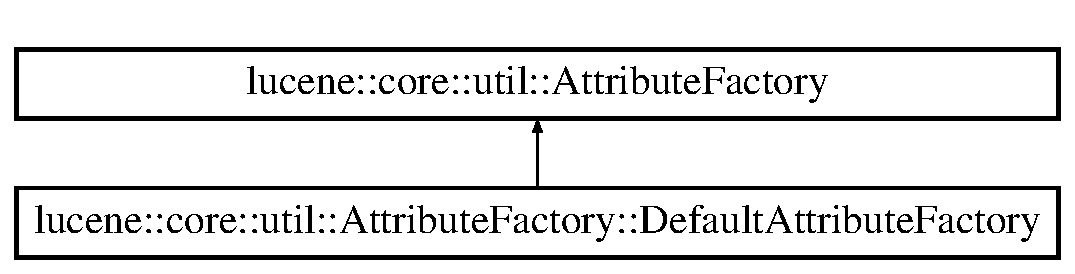
\includegraphics[height=2.000000cm]{classlucene_1_1core_1_1util_1_1AttributeFactory_1_1DefaultAttributeFactory}
\end{center}
\end{figure}
\subsection*{Public Member Functions}
\begin{DoxyCompactItemize}
\item 
\mbox{\hyperlink{classlucene_1_1core_1_1util_1_1AttributeFactory_1_1DefaultAttributeFactory_aa5249c715ab28f13919c833b779e6351}{Default\+Attribute\+Factory}} ()
\item 
virtual \mbox{\hyperlink{classlucene_1_1core_1_1util_1_1AttributeFactory_1_1DefaultAttributeFactory_a564f172e63c8c5c4f01cf9ec95a10e5f}{$\sim$\+Default\+Attribute\+Factory}} ()
\item 
\mbox{\hyperlink{classlucene_1_1core_1_1util_1_1AttributeImpl}{Attribute\+Impl}} $\ast$ \mbox{\hyperlink{classlucene_1_1core_1_1util_1_1AttributeFactory_1_1DefaultAttributeFactory_af9b68def67fc7995d2c5e9f3d1560f5e}{Create\+Attribute\+Instance}} (\mbox{\hyperlink{ZlibCrc32_8h_a2c212835823e3c54a8ab6d95c652660e}{const}} std\+::type\+\_\+index attr\+\_\+type\+\_\+id) override
\end{DoxyCompactItemize}
\subsection*{Additional Inherited Members}


\subsection{Constructor \& Destructor Documentation}
\mbox{\Hypertarget{classlucene_1_1core_1_1util_1_1AttributeFactory_1_1DefaultAttributeFactory_aa5249c715ab28f13919c833b779e6351}\label{classlucene_1_1core_1_1util_1_1AttributeFactory_1_1DefaultAttributeFactory_aa5249c715ab28f13919c833b779e6351}} 
\index{lucene\+::core\+::util\+::\+Attribute\+Factory\+::\+Default\+Attribute\+Factory@{lucene\+::core\+::util\+::\+Attribute\+Factory\+::\+Default\+Attribute\+Factory}!Default\+Attribute\+Factory@{Default\+Attribute\+Factory}}
\index{Default\+Attribute\+Factory@{Default\+Attribute\+Factory}!lucene\+::core\+::util\+::\+Attribute\+Factory\+::\+Default\+Attribute\+Factory@{lucene\+::core\+::util\+::\+Attribute\+Factory\+::\+Default\+Attribute\+Factory}}
\subsubsection{\texorpdfstring{Default\+Attribute\+Factory()}{DefaultAttributeFactory()}}
{\footnotesize\ttfamily \mbox{\hyperlink{classlucene_1_1core_1_1util_1_1AttributeFactory_1_1DefaultAttributeFactory}{Attribute\+Factory\+::\+Default\+Attribute\+Factory\+::\+Default\+Attribute\+Factory}} (\begin{DoxyParamCaption}{ }\end{DoxyParamCaption})}

\mbox{\Hypertarget{classlucene_1_1core_1_1util_1_1AttributeFactory_1_1DefaultAttributeFactory_a564f172e63c8c5c4f01cf9ec95a10e5f}\label{classlucene_1_1core_1_1util_1_1AttributeFactory_1_1DefaultAttributeFactory_a564f172e63c8c5c4f01cf9ec95a10e5f}} 
\index{lucene\+::core\+::util\+::\+Attribute\+Factory\+::\+Default\+Attribute\+Factory@{lucene\+::core\+::util\+::\+Attribute\+Factory\+::\+Default\+Attribute\+Factory}!````~Default\+Attribute\+Factory@{$\sim$\+Default\+Attribute\+Factory}}
\index{````~Default\+Attribute\+Factory@{$\sim$\+Default\+Attribute\+Factory}!lucene\+::core\+::util\+::\+Attribute\+Factory\+::\+Default\+Attribute\+Factory@{lucene\+::core\+::util\+::\+Attribute\+Factory\+::\+Default\+Attribute\+Factory}}
\subsubsection{\texorpdfstring{$\sim$\+Default\+Attribute\+Factory()}{~DefaultAttributeFactory()}}
{\footnotesize\ttfamily Attribute\+Factory\+::\+Default\+Attribute\+Factory\+::$\sim$\+Default\+Attribute\+Factory (\begin{DoxyParamCaption}{ }\end{DoxyParamCaption})\hspace{0.3cm}{\ttfamily [virtual]}}



\subsection{Member Function Documentation}
\mbox{\Hypertarget{classlucene_1_1core_1_1util_1_1AttributeFactory_1_1DefaultAttributeFactory_af9b68def67fc7995d2c5e9f3d1560f5e}\label{classlucene_1_1core_1_1util_1_1AttributeFactory_1_1DefaultAttributeFactory_af9b68def67fc7995d2c5e9f3d1560f5e}} 
\index{lucene\+::core\+::util\+::\+Attribute\+Factory\+::\+Default\+Attribute\+Factory@{lucene\+::core\+::util\+::\+Attribute\+Factory\+::\+Default\+Attribute\+Factory}!Create\+Attribute\+Instance@{Create\+Attribute\+Instance}}
\index{Create\+Attribute\+Instance@{Create\+Attribute\+Instance}!lucene\+::core\+::util\+::\+Attribute\+Factory\+::\+Default\+Attribute\+Factory@{lucene\+::core\+::util\+::\+Attribute\+Factory\+::\+Default\+Attribute\+Factory}}
\subsubsection{\texorpdfstring{Create\+Attribute\+Instance()}{CreateAttributeInstance()}}
{\footnotesize\ttfamily \mbox{\hyperlink{classlucene_1_1core_1_1util_1_1AttributeImpl}{Attribute\+Impl}} $\ast$ Attribute\+Factory\+::\+Default\+Attribute\+Factory\+::\+Create\+Attribute\+Instance (\begin{DoxyParamCaption}\item[{\mbox{\hyperlink{ZlibCrc32_8h_a2c212835823e3c54a8ab6d95c652660e}{const}} std\+::type\+\_\+index}]{attr\+\_\+type\+\_\+id }\end{DoxyParamCaption})\hspace{0.3cm}{\ttfamily [override]}, {\ttfamily [virtual]}}



Implements \mbox{\hyperlink{classlucene_1_1core_1_1util_1_1AttributeFactory_a88ccb9965ed78099379eaf9b1256abf3}{lucene\+::core\+::util\+::\+Attribute\+Factory}}.



The documentation for this class was generated from the following files\+:\begin{DoxyCompactItemize}
\item 
Util/\mbox{\hyperlink{Util_2Attribute_8h}{Attribute.\+h}}\item 
Util/\mbox{\hyperlink{Util_2Attribute_8cpp}{Attribute.\+cpp}}\end{DoxyCompactItemize}

\hypertarget{classDummyAnalyzer}{}\section{Dummy\+Analyzer Class Reference}
\label{classDummyAnalyzer}\index{Dummy\+Analyzer@{Dummy\+Analyzer}}
Inheritance diagram for Dummy\+Analyzer\+:\begin{figure}[H]
\begin{center}
\leavevmode
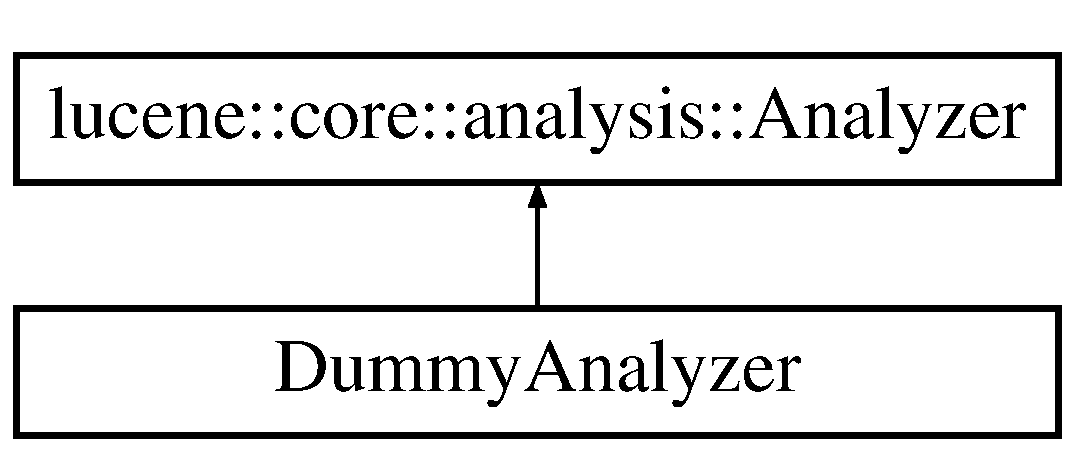
\includegraphics[height=2.000000cm]{classDummyAnalyzer}
\end{center}
\end{figure}
\subsection*{Protected Member Functions}
\begin{DoxyCompactItemize}
\item 
\mbox{\hyperlink{classlucene_1_1core_1_1analysis_1_1TokenStreamComponents}{Token\+Stream\+Components}} $\ast$ \mbox{\hyperlink{classDummyAnalyzer_aeeb24aa6449d4bf7c4adc6a5c63a5c0e}{Create\+Components}} (\mbox{\hyperlink{ZlibCrc32_8h_a2c212835823e3c54a8ab6d95c652660e}{const}} std\+::string \&field\+\_\+name)
\end{DoxyCompactItemize}
\subsection*{Additional Inherited Members}


\subsection{Member Function Documentation}
\mbox{\Hypertarget{classDummyAnalyzer_aeeb24aa6449d4bf7c4adc6a5c63a5c0e}\label{classDummyAnalyzer_aeeb24aa6449d4bf7c4adc6a5c63a5c0e}} 
\index{Dummy\+Analyzer@{Dummy\+Analyzer}!Create\+Components@{Create\+Components}}
\index{Create\+Components@{Create\+Components}!Dummy\+Analyzer@{Dummy\+Analyzer}}
\subsubsection{\texorpdfstring{Create\+Components()}{CreateComponents()}}
{\footnotesize\ttfamily \mbox{\hyperlink{classlucene_1_1core_1_1analysis_1_1TokenStreamComponents}{Token\+Stream\+Components}}$\ast$ Dummy\+Analyzer\+::\+Create\+Components (\begin{DoxyParamCaption}\item[{\mbox{\hyperlink{ZlibCrc32_8h_a2c212835823e3c54a8ab6d95c652660e}{const}} std\+::string \&}]{field\+\_\+name }\end{DoxyParamCaption})\hspace{0.3cm}{\ttfamily [inline]}, {\ttfamily [protected]}, {\ttfamily [virtual]}}



Implements \mbox{\hyperlink{classlucene_1_1core_1_1analysis_1_1Analyzer_a9b7dc3c598057fbf4e9b5f48066cb54a}{lucene\+::core\+::analysis\+::\+Analyzer}}.



The documentation for this class was generated from the following file\+:\begin{DoxyCompactItemize}
\item 
Analysis/tests/\mbox{\hyperlink{AnalyzerTests_8cpp}{Analyzer\+Tests.\+cpp}}\end{DoxyCompactItemize}

\hypertarget{classDummyClass}{}\section{Dummy\+Class Class Reference}
\label{classDummyClass}\index{Dummy\+Class@{Dummy\+Class}}


The documentation for this class was generated from the following file\+:\begin{DoxyCompactItemize}
\item 
Util/tests/\mbox{\hyperlink{ConcurrencyTests_8cpp}{Concurrency\+Tests.\+cpp}}\end{DoxyCompactItemize}

\hypertarget{classDummyTokenFilter}{}\section{Dummy\+Token\+Filter Class Reference}
\label{classDummyTokenFilter}\index{Dummy\+Token\+Filter@{Dummy\+Token\+Filter}}
Inheritance diagram for Dummy\+Token\+Filter\+:\begin{figure}[H]
\begin{center}
\leavevmode
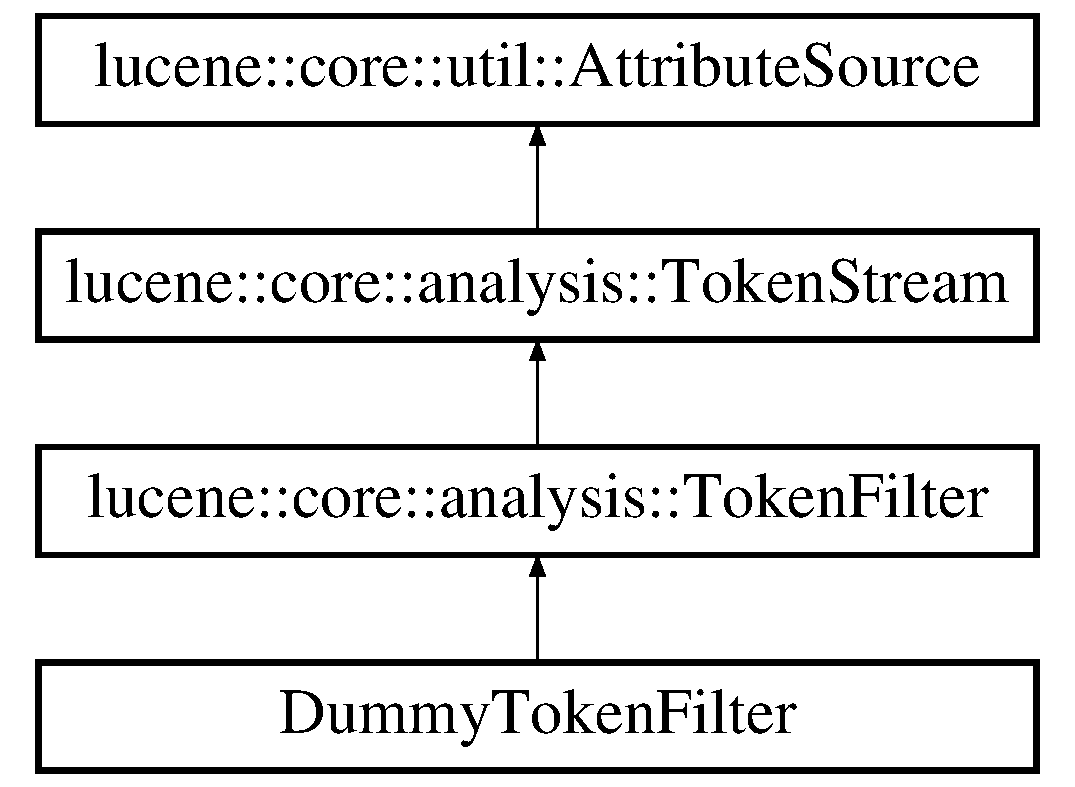
\includegraphics[height=4.000000cm]{classDummyTokenFilter}
\end{center}
\end{figure}
\subsection*{Public Member Functions}
\begin{DoxyCompactItemize}
\item 
\mbox{\hyperlink{classDummyTokenFilter_a9662eaa1241759e097feadba88df7726}{Dummy\+Token\+Filter}} (std\+::shared\+\_\+ptr$<$ \mbox{\hyperlink{classlucene_1_1core_1_1analysis_1_1TokenStream}{Token\+Stream}} $>$ in)
\item 
\mbox{\hyperlink{classDummyTokenFilter_a159c2c68741206a402c7b80c3f0ef14f}{Dummy\+Token\+Filter}} (\mbox{\hyperlink{classlucene_1_1core_1_1analysis_1_1TokenStream}{Token\+Stream}} $\ast$in)
\item 
bool \mbox{\hyperlink{classDummyTokenFilter_a6a57ec2684cc58f61ec807bbebabae63}{Increment\+Token}} ()
\end{DoxyCompactItemize}
\subsection*{Public Attributes}
\begin{DoxyCompactItemize}
\item 
std\+::shared\+\_\+ptr$<$ \mbox{\hyperlink{classlucene_1_1core_1_1analysis_1_1tokenattributes_1_1CharTermAttribute}{Char\+Term\+Attribute}} $>$ \mbox{\hyperlink{classDummyTokenFilter_ab057e032de3b055c554c4ab4abf1c3da}{char\+\_\+term\+\_\+attr}}
\end{DoxyCompactItemize}
\subsection*{Additional Inherited Members}


\subsection{Constructor \& Destructor Documentation}
\mbox{\Hypertarget{classDummyTokenFilter_a9662eaa1241759e097feadba88df7726}\label{classDummyTokenFilter_a9662eaa1241759e097feadba88df7726}} 
\index{Dummy\+Token\+Filter@{Dummy\+Token\+Filter}!Dummy\+Token\+Filter@{Dummy\+Token\+Filter}}
\index{Dummy\+Token\+Filter@{Dummy\+Token\+Filter}!Dummy\+Token\+Filter@{Dummy\+Token\+Filter}}
\subsubsection{\texorpdfstring{Dummy\+Token\+Filter()}{DummyTokenFilter()}\hspace{0.1cm}{\footnotesize\ttfamily [1/2]}}
{\footnotesize\ttfamily Dummy\+Token\+Filter\+::\+Dummy\+Token\+Filter (\begin{DoxyParamCaption}\item[{std\+::shared\+\_\+ptr$<$ \mbox{\hyperlink{classlucene_1_1core_1_1analysis_1_1TokenStream}{Token\+Stream}} $>$}]{in }\end{DoxyParamCaption})\hspace{0.3cm}{\ttfamily [inline]}, {\ttfamily [explicit]}}

\mbox{\Hypertarget{classDummyTokenFilter_a159c2c68741206a402c7b80c3f0ef14f}\label{classDummyTokenFilter_a159c2c68741206a402c7b80c3f0ef14f}} 
\index{Dummy\+Token\+Filter@{Dummy\+Token\+Filter}!Dummy\+Token\+Filter@{Dummy\+Token\+Filter}}
\index{Dummy\+Token\+Filter@{Dummy\+Token\+Filter}!Dummy\+Token\+Filter@{Dummy\+Token\+Filter}}
\subsubsection{\texorpdfstring{Dummy\+Token\+Filter()}{DummyTokenFilter()}\hspace{0.1cm}{\footnotesize\ttfamily [2/2]}}
{\footnotesize\ttfamily Dummy\+Token\+Filter\+::\+Dummy\+Token\+Filter (\begin{DoxyParamCaption}\item[{\mbox{\hyperlink{classlucene_1_1core_1_1analysis_1_1TokenStream}{Token\+Stream}} $\ast$}]{in }\end{DoxyParamCaption})\hspace{0.3cm}{\ttfamily [inline]}, {\ttfamily [explicit]}}



\subsection{Member Function Documentation}
\mbox{\Hypertarget{classDummyTokenFilter_a6a57ec2684cc58f61ec807bbebabae63}\label{classDummyTokenFilter_a6a57ec2684cc58f61ec807bbebabae63}} 
\index{Dummy\+Token\+Filter@{Dummy\+Token\+Filter}!Increment\+Token@{Increment\+Token}}
\index{Increment\+Token@{Increment\+Token}!Dummy\+Token\+Filter@{Dummy\+Token\+Filter}}
\subsubsection{\texorpdfstring{Increment\+Token()}{IncrementToken()}}
{\footnotesize\ttfamily bool Dummy\+Token\+Filter\+::\+Increment\+Token (\begin{DoxyParamCaption}{ }\end{DoxyParamCaption})\hspace{0.3cm}{\ttfamily [inline]}, {\ttfamily [virtual]}}



Implements \mbox{\hyperlink{classlucene_1_1core_1_1analysis_1_1TokenStream_a614d4ea24a354d6f4354b4941b5124e2}{lucene\+::core\+::analysis\+::\+Token\+Stream}}.



\subsection{Member Data Documentation}
\mbox{\Hypertarget{classDummyTokenFilter_ab057e032de3b055c554c4ab4abf1c3da}\label{classDummyTokenFilter_ab057e032de3b055c554c4ab4abf1c3da}} 
\index{Dummy\+Token\+Filter@{Dummy\+Token\+Filter}!char\+\_\+term\+\_\+attr@{char\+\_\+term\+\_\+attr}}
\index{char\+\_\+term\+\_\+attr@{char\+\_\+term\+\_\+attr}!Dummy\+Token\+Filter@{Dummy\+Token\+Filter}}
\subsubsection{\texorpdfstring{char\+\_\+term\+\_\+attr}{char\_term\_attr}}
{\footnotesize\ttfamily std\+::shared\+\_\+ptr$<$\mbox{\hyperlink{classlucene_1_1core_1_1analysis_1_1tokenattributes_1_1CharTermAttribute}{Char\+Term\+Attribute}}$>$ Dummy\+Token\+Filter\+::char\+\_\+term\+\_\+attr}



The documentation for this class was generated from the following file\+:\begin{DoxyCompactItemize}
\item 
Analysis/tests/\mbox{\hyperlink{AnalyzerTests_8cpp}{Analyzer\+Tests.\+cpp}}\end{DoxyCompactItemize}

\hypertarget{classDummyTokenizer}{}\section{Dummy\+Tokenizer Class Reference}
\label{classDummyTokenizer}\index{Dummy\+Tokenizer@{Dummy\+Tokenizer}}
Inheritance diagram for Dummy\+Tokenizer\+:\begin{figure}[H]
\begin{center}
\leavevmode
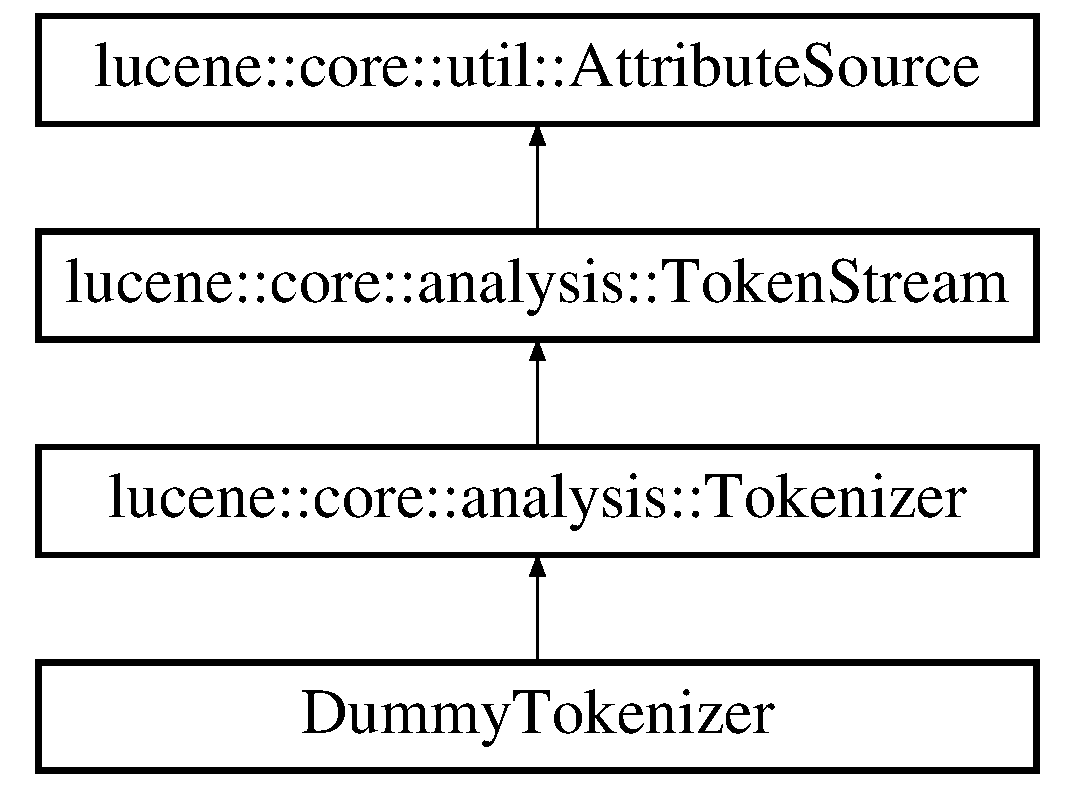
\includegraphics[height=4.000000cm]{classDummyTokenizer}
\end{center}
\end{figure}
\subsection*{Public Member Functions}
\begin{DoxyCompactItemize}
\item 
\mbox{\hyperlink{classDummyTokenizer_a42b1fc7050177a061fc4cd35fa3ddee3}{Dummy\+Tokenizer}} ()
\item 
bool \mbox{\hyperlink{classDummyTokenizer_a11402de15d04027b30ce918814e1723d}{Increment\+Token}} ()
\end{DoxyCompactItemize}
\subsection*{Public Attributes}
\begin{DoxyCompactItemize}
\item 
std\+::shared\+\_\+ptr$<$ \mbox{\hyperlink{classlucene_1_1core_1_1analysis_1_1tokenattributes_1_1CharTermAttribute}{Char\+Term\+Attribute}} $>$ \mbox{\hyperlink{classDummyTokenizer_a6bfd1c116c7c2f98be9a605dc985f534}{char\+\_\+term\+\_\+attr}}
\item 
bool \mbox{\hyperlink{classDummyTokenizer_aa9c8e2fcc234b7adcc1d1f1c9dc1716f}{read}}
\end{DoxyCompactItemize}
\subsection*{Additional Inherited Members}


\subsection{Constructor \& Destructor Documentation}
\mbox{\Hypertarget{classDummyTokenizer_a42b1fc7050177a061fc4cd35fa3ddee3}\label{classDummyTokenizer_a42b1fc7050177a061fc4cd35fa3ddee3}} 
\index{Dummy\+Tokenizer@{Dummy\+Tokenizer}!Dummy\+Tokenizer@{Dummy\+Tokenizer}}
\index{Dummy\+Tokenizer@{Dummy\+Tokenizer}!Dummy\+Tokenizer@{Dummy\+Tokenizer}}
\subsubsection{\texorpdfstring{Dummy\+Tokenizer()}{DummyTokenizer()}}
{\footnotesize\ttfamily Dummy\+Tokenizer\+::\+Dummy\+Tokenizer (\begin{DoxyParamCaption}{ }\end{DoxyParamCaption})\hspace{0.3cm}{\ttfamily [inline]}}



\subsection{Member Function Documentation}
\mbox{\Hypertarget{classDummyTokenizer_a11402de15d04027b30ce918814e1723d}\label{classDummyTokenizer_a11402de15d04027b30ce918814e1723d}} 
\index{Dummy\+Tokenizer@{Dummy\+Tokenizer}!Increment\+Token@{Increment\+Token}}
\index{Increment\+Token@{Increment\+Token}!Dummy\+Tokenizer@{Dummy\+Tokenizer}}
\subsubsection{\texorpdfstring{Increment\+Token()}{IncrementToken()}}
{\footnotesize\ttfamily bool Dummy\+Tokenizer\+::\+Increment\+Token (\begin{DoxyParamCaption}{ }\end{DoxyParamCaption})\hspace{0.3cm}{\ttfamily [inline]}, {\ttfamily [virtual]}}



Implements \mbox{\hyperlink{classlucene_1_1core_1_1analysis_1_1TokenStream_a614d4ea24a354d6f4354b4941b5124e2}{lucene\+::core\+::analysis\+::\+Token\+Stream}}.



\subsection{Member Data Documentation}
\mbox{\Hypertarget{classDummyTokenizer_a6bfd1c116c7c2f98be9a605dc985f534}\label{classDummyTokenizer_a6bfd1c116c7c2f98be9a605dc985f534}} 
\index{Dummy\+Tokenizer@{Dummy\+Tokenizer}!char\+\_\+term\+\_\+attr@{char\+\_\+term\+\_\+attr}}
\index{char\+\_\+term\+\_\+attr@{char\+\_\+term\+\_\+attr}!Dummy\+Tokenizer@{Dummy\+Tokenizer}}
\subsubsection{\texorpdfstring{char\+\_\+term\+\_\+attr}{char\_term\_attr}}
{\footnotesize\ttfamily std\+::shared\+\_\+ptr$<$\mbox{\hyperlink{classlucene_1_1core_1_1analysis_1_1tokenattributes_1_1CharTermAttribute}{Char\+Term\+Attribute}}$>$ Dummy\+Tokenizer\+::char\+\_\+term\+\_\+attr}

\mbox{\Hypertarget{classDummyTokenizer_aa9c8e2fcc234b7adcc1d1f1c9dc1716f}\label{classDummyTokenizer_aa9c8e2fcc234b7adcc1d1f1c9dc1716f}} 
\index{Dummy\+Tokenizer@{Dummy\+Tokenizer}!read@{read}}
\index{read@{read}!Dummy\+Tokenizer@{Dummy\+Tokenizer}}
\subsubsection{\texorpdfstring{read}{read}}
{\footnotesize\ttfamily bool Dummy\+Tokenizer\+::read}



The documentation for this class was generated from the following file\+:\begin{DoxyCompactItemize}
\item 
Analysis/tests/\mbox{\hyperlink{AnalyzerTests_8cpp}{Analyzer\+Tests.\+cpp}}\end{DoxyCompactItemize}

\hypertarget{classlucene_1_1core_1_1util_1_1EmptyThreadLocalException}{}\section{lucene\+:\+:core\+:\+:util\+:\+:Empty\+Thread\+Local\+Exception Class Reference}
\label{classlucene_1_1core_1_1util_1_1EmptyThreadLocalException}\index{lucene\+::core\+::util\+::\+Empty\+Thread\+Local\+Exception@{lucene\+::core\+::util\+::\+Empty\+Thread\+Local\+Exception}}


{\ttfamily \#include $<$Concurrency.\+h$>$}

Inheritance diagram for lucene\+:\+:core\+:\+:util\+:\+:Empty\+Thread\+Local\+Exception\+:\begin{figure}[H]
\begin{center}
\leavevmode
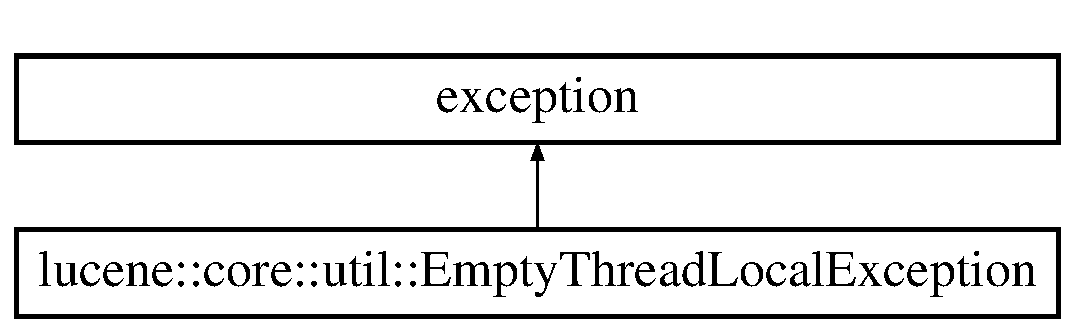
\includegraphics[height=2.000000cm]{classlucene_1_1core_1_1util_1_1EmptyThreadLocalException}
\end{center}
\end{figure}
\subsection*{Public Member Functions}
\begin{DoxyCompactItemize}
\item 
\mbox{\hyperlink{classlucene_1_1core_1_1util_1_1EmptyThreadLocalException_a241a95d08b41259f7cb3c5d4a399b098}{Empty\+Thread\+Local\+Exception}} ()
\item 
virtual \mbox{\hyperlink{ZlibCrc32_8h_a2c212835823e3c54a8ab6d95c652660e}{const}} char $\ast$ \mbox{\hyperlink{classlucene_1_1core_1_1util_1_1EmptyThreadLocalException_a33f16d7924d5b7b094c1af85ff8268ef}{what}} () \mbox{\hyperlink{ZlibCrc32_8h_a2c212835823e3c54a8ab6d95c652660e}{const}}  throw ()
\end{DoxyCompactItemize}


\subsection{Constructor \& Destructor Documentation}
\mbox{\Hypertarget{classlucene_1_1core_1_1util_1_1EmptyThreadLocalException_a241a95d08b41259f7cb3c5d4a399b098}\label{classlucene_1_1core_1_1util_1_1EmptyThreadLocalException_a241a95d08b41259f7cb3c5d4a399b098}} 
\index{lucene\+::core\+::util\+::\+Empty\+Thread\+Local\+Exception@{lucene\+::core\+::util\+::\+Empty\+Thread\+Local\+Exception}!Empty\+Thread\+Local\+Exception@{Empty\+Thread\+Local\+Exception}}
\index{Empty\+Thread\+Local\+Exception@{Empty\+Thread\+Local\+Exception}!lucene\+::core\+::util\+::\+Empty\+Thread\+Local\+Exception@{lucene\+::core\+::util\+::\+Empty\+Thread\+Local\+Exception}}
\subsubsection{\texorpdfstring{Empty\+Thread\+Local\+Exception()}{EmptyThreadLocalException()}}
{\footnotesize\ttfamily lucene\+::core\+::util\+::\+Empty\+Thread\+Local\+Exception\+::\+Empty\+Thread\+Local\+Exception (\begin{DoxyParamCaption}{ }\end{DoxyParamCaption})\hspace{0.3cm}{\ttfamily [inline]}}



\subsection{Member Function Documentation}
\mbox{\Hypertarget{classlucene_1_1core_1_1util_1_1EmptyThreadLocalException_a33f16d7924d5b7b094c1af85ff8268ef}\label{classlucene_1_1core_1_1util_1_1EmptyThreadLocalException_a33f16d7924d5b7b094c1af85ff8268ef}} 
\index{lucene\+::core\+::util\+::\+Empty\+Thread\+Local\+Exception@{lucene\+::core\+::util\+::\+Empty\+Thread\+Local\+Exception}!what@{what}}
\index{what@{what}!lucene\+::core\+::util\+::\+Empty\+Thread\+Local\+Exception@{lucene\+::core\+::util\+::\+Empty\+Thread\+Local\+Exception}}
\subsubsection{\texorpdfstring{what()}{what()}}
{\footnotesize\ttfamily virtual \mbox{\hyperlink{ZlibCrc32_8h_a2c212835823e3c54a8ab6d95c652660e}{const}} char$\ast$ lucene\+::core\+::util\+::\+Empty\+Thread\+Local\+Exception\+::what (\begin{DoxyParamCaption}{ }\end{DoxyParamCaption}) const throw  ) \hspace{0.3cm}{\ttfamily [inline]}, {\ttfamily [virtual]}}



The documentation for this class was generated from the following file\+:\begin{DoxyCompactItemize}
\item 
Util/\mbox{\hyperlink{Concurrency_8h}{Concurrency.\+h}}\end{DoxyCompactItemize}

\hypertarget{classlucene_1_1core_1_1analysis_1_1FilteringTokenFilter}{}\section{lucene\+:\+:core\+:\+:analysis\+:\+:Filtering\+Token\+Filter Class Reference}
\label{classlucene_1_1core_1_1analysis_1_1FilteringTokenFilter}\index{lucene\+::core\+::analysis\+::\+Filtering\+Token\+Filter@{lucene\+::core\+::analysis\+::\+Filtering\+Token\+Filter}}


{\ttfamily \#include $<$Token\+Stream.\+h$>$}

Inheritance diagram for lucene\+:\+:core\+:\+:analysis\+:\+:Filtering\+Token\+Filter\+:\begin{figure}[H]
\begin{center}
\leavevmode
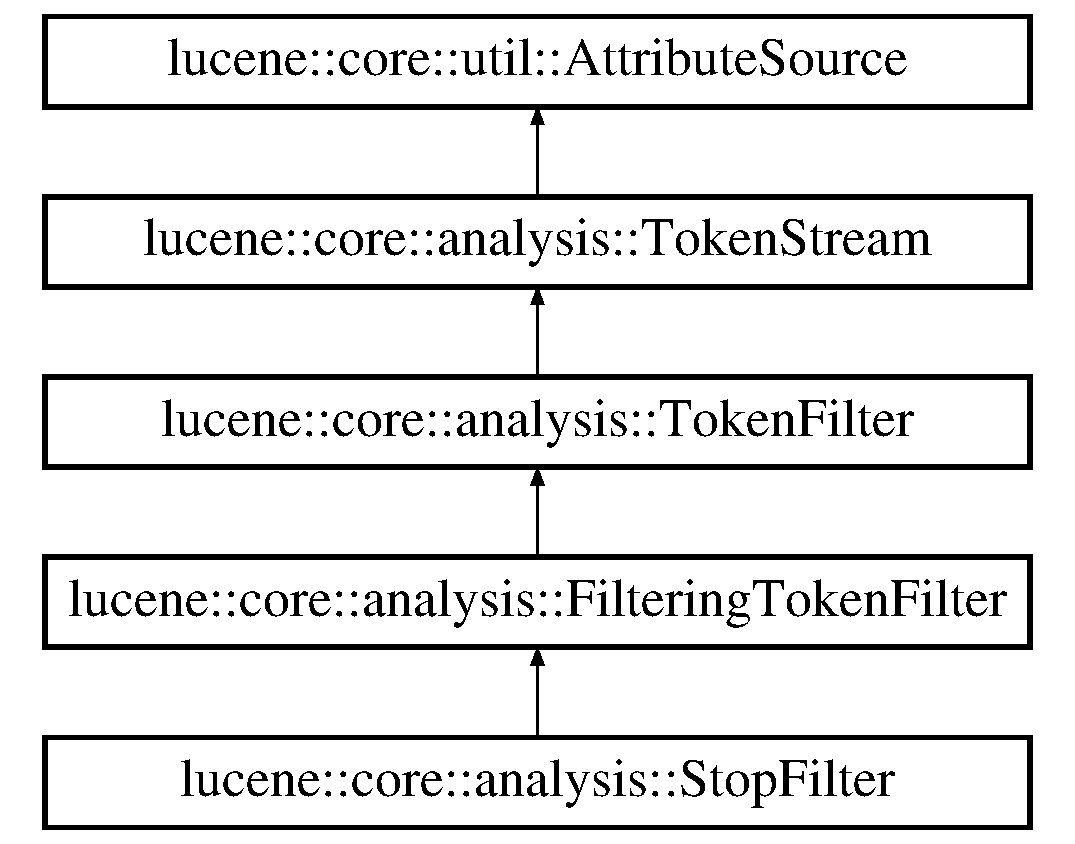
\includegraphics[height=5.000000cm]{classlucene_1_1core_1_1analysis_1_1FilteringTokenFilter}
\end{center}
\end{figure}
\subsection*{Public Member Functions}
\begin{DoxyCompactItemize}
\item 
\mbox{\hyperlink{classlucene_1_1core_1_1analysis_1_1FilteringTokenFilter_ac5ae5016927281bfd3cff1161b3a36b4}{Filtering\+Token\+Filter}} (std\+::shared\+\_\+ptr$<$ \mbox{\hyperlink{classlucene_1_1core_1_1analysis_1_1TokenStream}{Token\+Stream}} $>$ in)
\item 
\mbox{\hyperlink{classlucene_1_1core_1_1analysis_1_1FilteringTokenFilter_a6ad64db0fcf39d585e28c8f1d44f7617}{Filtering\+Token\+Filter}} (\mbox{\hyperlink{classlucene_1_1core_1_1analysis_1_1TokenStream}{Token\+Stream}} $\ast$in)
\item 
virtual \mbox{\hyperlink{classlucene_1_1core_1_1analysis_1_1FilteringTokenFilter_a52769c366f866d8d48fe2bdb1a438f50}{$\sim$\+Filtering\+Token\+Filter}} ()
\item 
bool \mbox{\hyperlink{classlucene_1_1core_1_1analysis_1_1FilteringTokenFilter_aa1956aa94779023b3f97b667bd819734}{Increment\+Token}} () override
\item 
void \mbox{\hyperlink{classlucene_1_1core_1_1analysis_1_1FilteringTokenFilter_ab85e4deab22d9dedd7ccb7b1f4750400}{Reset}} () override
\item 
void \mbox{\hyperlink{classlucene_1_1core_1_1analysis_1_1FilteringTokenFilter_adf6b7aac9634afdffe1800a369753688}{End}} () override
\end{DoxyCompactItemize}
\subsection*{Protected Member Functions}
\begin{DoxyCompactItemize}
\item 
virtual bool \mbox{\hyperlink{classlucene_1_1core_1_1analysis_1_1FilteringTokenFilter_a4a2fb2dd2d3bda8eb6cd0d5b14a4ab92}{Accept}} ()=0
\end{DoxyCompactItemize}
\subsection*{Private Attributes}
\begin{DoxyCompactItemize}
\item 
std\+::shared\+\_\+ptr$<$ \mbox{\hyperlink{classlucene_1_1core_1_1analysis_1_1tokenattributes_1_1PositionIncrementAttribute}{tokenattributes\+::\+Position\+Increment\+Attribute}} $>$ \mbox{\hyperlink{classlucene_1_1core_1_1analysis_1_1FilteringTokenFilter_a49bf3c192e5ac9389c9ada77080d75c7}{pos\+\_\+incr\+\_\+attr}}
\item 
int32\+\_\+t \mbox{\hyperlink{classlucene_1_1core_1_1analysis_1_1FilteringTokenFilter_ac2fdc9a36ad1526780daf709595ba6b2}{skipped\+\_\+positions}}
\end{DoxyCompactItemize}
\subsection*{Additional Inherited Members}


\subsection{Constructor \& Destructor Documentation}
\mbox{\Hypertarget{classlucene_1_1core_1_1analysis_1_1FilteringTokenFilter_ac5ae5016927281bfd3cff1161b3a36b4}\label{classlucene_1_1core_1_1analysis_1_1FilteringTokenFilter_ac5ae5016927281bfd3cff1161b3a36b4}} 
\index{lucene\+::core\+::analysis\+::\+Filtering\+Token\+Filter@{lucene\+::core\+::analysis\+::\+Filtering\+Token\+Filter}!Filtering\+Token\+Filter@{Filtering\+Token\+Filter}}
\index{Filtering\+Token\+Filter@{Filtering\+Token\+Filter}!lucene\+::core\+::analysis\+::\+Filtering\+Token\+Filter@{lucene\+::core\+::analysis\+::\+Filtering\+Token\+Filter}}
\subsubsection{\texorpdfstring{Filtering\+Token\+Filter()}{FilteringTokenFilter()}\hspace{0.1cm}{\footnotesize\ttfamily [1/2]}}
{\footnotesize\ttfamily lucene\+::core\+::analysis\+::\+Filtering\+Token\+Filter\+::\+Filtering\+Token\+Filter (\begin{DoxyParamCaption}\item[{std\+::shared\+\_\+ptr$<$ \mbox{\hyperlink{classlucene_1_1core_1_1analysis_1_1TokenStream}{Token\+Stream}} $>$}]{in }\end{DoxyParamCaption})\hspace{0.3cm}{\ttfamily [explicit]}}

\mbox{\Hypertarget{classlucene_1_1core_1_1analysis_1_1FilteringTokenFilter_a6ad64db0fcf39d585e28c8f1d44f7617}\label{classlucene_1_1core_1_1analysis_1_1FilteringTokenFilter_a6ad64db0fcf39d585e28c8f1d44f7617}} 
\index{lucene\+::core\+::analysis\+::\+Filtering\+Token\+Filter@{lucene\+::core\+::analysis\+::\+Filtering\+Token\+Filter}!Filtering\+Token\+Filter@{Filtering\+Token\+Filter}}
\index{Filtering\+Token\+Filter@{Filtering\+Token\+Filter}!lucene\+::core\+::analysis\+::\+Filtering\+Token\+Filter@{lucene\+::core\+::analysis\+::\+Filtering\+Token\+Filter}}
\subsubsection{\texorpdfstring{Filtering\+Token\+Filter()}{FilteringTokenFilter()}\hspace{0.1cm}{\footnotesize\ttfamily [2/2]}}
{\footnotesize\ttfamily Filtering\+Token\+Filter\+::\+Filtering\+Token\+Filter (\begin{DoxyParamCaption}\item[{\mbox{\hyperlink{classlucene_1_1core_1_1analysis_1_1TokenStream}{Token\+Stream}} $\ast$}]{in }\end{DoxyParamCaption})\hspace{0.3cm}{\ttfamily [explicit]}}

\mbox{\hyperlink{classlucene_1_1core_1_1analysis_1_1FilteringTokenFilter}{Filtering\+Token\+Filter}} \mbox{\Hypertarget{classlucene_1_1core_1_1analysis_1_1FilteringTokenFilter_a52769c366f866d8d48fe2bdb1a438f50}\label{classlucene_1_1core_1_1analysis_1_1FilteringTokenFilter_a52769c366f866d8d48fe2bdb1a438f50}} 
\index{lucene\+::core\+::analysis\+::\+Filtering\+Token\+Filter@{lucene\+::core\+::analysis\+::\+Filtering\+Token\+Filter}!````~Filtering\+Token\+Filter@{$\sim$\+Filtering\+Token\+Filter}}
\index{````~Filtering\+Token\+Filter@{$\sim$\+Filtering\+Token\+Filter}!lucene\+::core\+::analysis\+::\+Filtering\+Token\+Filter@{lucene\+::core\+::analysis\+::\+Filtering\+Token\+Filter}}
\subsubsection{\texorpdfstring{$\sim$\+Filtering\+Token\+Filter()}{~FilteringTokenFilter()}}
{\footnotesize\ttfamily Filtering\+Token\+Filter\+::$\sim$\+Filtering\+Token\+Filter (\begin{DoxyParamCaption}{ }\end{DoxyParamCaption})\hspace{0.3cm}{\ttfamily [virtual]}}



\subsection{Member Function Documentation}
\mbox{\Hypertarget{classlucene_1_1core_1_1analysis_1_1FilteringTokenFilter_a4a2fb2dd2d3bda8eb6cd0d5b14a4ab92}\label{classlucene_1_1core_1_1analysis_1_1FilteringTokenFilter_a4a2fb2dd2d3bda8eb6cd0d5b14a4ab92}} 
\index{lucene\+::core\+::analysis\+::\+Filtering\+Token\+Filter@{lucene\+::core\+::analysis\+::\+Filtering\+Token\+Filter}!Accept@{Accept}}
\index{Accept@{Accept}!lucene\+::core\+::analysis\+::\+Filtering\+Token\+Filter@{lucene\+::core\+::analysis\+::\+Filtering\+Token\+Filter}}
\subsubsection{\texorpdfstring{Accept()}{Accept()}}
{\footnotesize\ttfamily virtual bool lucene\+::core\+::analysis\+::\+Filtering\+Token\+Filter\+::\+Accept (\begin{DoxyParamCaption}{ }\end{DoxyParamCaption})\hspace{0.3cm}{\ttfamily [protected]}, {\ttfamily [pure virtual]}}



Implemented in \mbox{\hyperlink{classlucene_1_1core_1_1analysis_1_1StopFilter_af05114955fb7b1deb340a7fe1e07735e}{lucene\+::core\+::analysis\+::\+Stop\+Filter}}.

\mbox{\Hypertarget{classlucene_1_1core_1_1analysis_1_1FilteringTokenFilter_adf6b7aac9634afdffe1800a369753688}\label{classlucene_1_1core_1_1analysis_1_1FilteringTokenFilter_adf6b7aac9634afdffe1800a369753688}} 
\index{lucene\+::core\+::analysis\+::\+Filtering\+Token\+Filter@{lucene\+::core\+::analysis\+::\+Filtering\+Token\+Filter}!End@{End}}
\index{End@{End}!lucene\+::core\+::analysis\+::\+Filtering\+Token\+Filter@{lucene\+::core\+::analysis\+::\+Filtering\+Token\+Filter}}
\subsubsection{\texorpdfstring{End()}{End()}}
{\footnotesize\ttfamily void Filtering\+Token\+Filter\+::\+End (\begin{DoxyParamCaption}{ }\end{DoxyParamCaption})\hspace{0.3cm}{\ttfamily [override]}, {\ttfamily [virtual]}}



Reimplemented from \mbox{\hyperlink{classlucene_1_1core_1_1analysis_1_1TokenFilter_ad2e29dd32aa4df385d0f290f10f20721}{lucene\+::core\+::analysis\+::\+Token\+Filter}}.

\mbox{\Hypertarget{classlucene_1_1core_1_1analysis_1_1FilteringTokenFilter_aa1956aa94779023b3f97b667bd819734}\label{classlucene_1_1core_1_1analysis_1_1FilteringTokenFilter_aa1956aa94779023b3f97b667bd819734}} 
\index{lucene\+::core\+::analysis\+::\+Filtering\+Token\+Filter@{lucene\+::core\+::analysis\+::\+Filtering\+Token\+Filter}!Increment\+Token@{Increment\+Token}}
\index{Increment\+Token@{Increment\+Token}!lucene\+::core\+::analysis\+::\+Filtering\+Token\+Filter@{lucene\+::core\+::analysis\+::\+Filtering\+Token\+Filter}}
\subsubsection{\texorpdfstring{Increment\+Token()}{IncrementToken()}}
{\footnotesize\ttfamily bool Filtering\+Token\+Filter\+::\+Increment\+Token (\begin{DoxyParamCaption}{ }\end{DoxyParamCaption})\hspace{0.3cm}{\ttfamily [override]}, {\ttfamily [virtual]}}



Implements \mbox{\hyperlink{classlucene_1_1core_1_1analysis_1_1TokenStream_a614d4ea24a354d6f4354b4941b5124e2}{lucene\+::core\+::analysis\+::\+Token\+Stream}}.

\mbox{\Hypertarget{classlucene_1_1core_1_1analysis_1_1FilteringTokenFilter_ab85e4deab22d9dedd7ccb7b1f4750400}\label{classlucene_1_1core_1_1analysis_1_1FilteringTokenFilter_ab85e4deab22d9dedd7ccb7b1f4750400}} 
\index{lucene\+::core\+::analysis\+::\+Filtering\+Token\+Filter@{lucene\+::core\+::analysis\+::\+Filtering\+Token\+Filter}!Reset@{Reset}}
\index{Reset@{Reset}!lucene\+::core\+::analysis\+::\+Filtering\+Token\+Filter@{lucene\+::core\+::analysis\+::\+Filtering\+Token\+Filter}}
\subsubsection{\texorpdfstring{Reset()}{Reset()}}
{\footnotesize\ttfamily void Filtering\+Token\+Filter\+::\+Reset (\begin{DoxyParamCaption}{ }\end{DoxyParamCaption})\hspace{0.3cm}{\ttfamily [override]}, {\ttfamily [virtual]}}



Reimplemented from \mbox{\hyperlink{classlucene_1_1core_1_1analysis_1_1TokenFilter_a0671ee825db7735a7b72b7a27a457ed9}{lucene\+::core\+::analysis\+::\+Token\+Filter}}.



\subsection{Member Data Documentation}
\mbox{\Hypertarget{classlucene_1_1core_1_1analysis_1_1FilteringTokenFilter_a49bf3c192e5ac9389c9ada77080d75c7}\label{classlucene_1_1core_1_1analysis_1_1FilteringTokenFilter_a49bf3c192e5ac9389c9ada77080d75c7}} 
\index{lucene\+::core\+::analysis\+::\+Filtering\+Token\+Filter@{lucene\+::core\+::analysis\+::\+Filtering\+Token\+Filter}!pos\+\_\+incr\+\_\+attr@{pos\+\_\+incr\+\_\+attr}}
\index{pos\+\_\+incr\+\_\+attr@{pos\+\_\+incr\+\_\+attr}!lucene\+::core\+::analysis\+::\+Filtering\+Token\+Filter@{lucene\+::core\+::analysis\+::\+Filtering\+Token\+Filter}}
\subsubsection{\texorpdfstring{pos\+\_\+incr\+\_\+attr}{pos\_incr\_attr}}
{\footnotesize\ttfamily std\+::shared\+\_\+ptr$<$\mbox{\hyperlink{classlucene_1_1core_1_1analysis_1_1tokenattributes_1_1PositionIncrementAttribute}{tokenattributes\+::\+Position\+Increment\+Attribute}}$>$ lucene\+::core\+::analysis\+::\+Filtering\+Token\+Filter\+::pos\+\_\+incr\+\_\+attr\hspace{0.3cm}{\ttfamily [private]}}

\mbox{\Hypertarget{classlucene_1_1core_1_1analysis_1_1FilteringTokenFilter_ac2fdc9a36ad1526780daf709595ba6b2}\label{classlucene_1_1core_1_1analysis_1_1FilteringTokenFilter_ac2fdc9a36ad1526780daf709595ba6b2}} 
\index{lucene\+::core\+::analysis\+::\+Filtering\+Token\+Filter@{lucene\+::core\+::analysis\+::\+Filtering\+Token\+Filter}!skipped\+\_\+positions@{skipped\+\_\+positions}}
\index{skipped\+\_\+positions@{skipped\+\_\+positions}!lucene\+::core\+::analysis\+::\+Filtering\+Token\+Filter@{lucene\+::core\+::analysis\+::\+Filtering\+Token\+Filter}}
\subsubsection{\texorpdfstring{skipped\+\_\+positions}{skipped\_positions}}
{\footnotesize\ttfamily int32\+\_\+t lucene\+::core\+::analysis\+::\+Filtering\+Token\+Filter\+::skipped\+\_\+positions\hspace{0.3cm}{\ttfamily [private]}}



The documentation for this class was generated from the following files\+:\begin{DoxyCompactItemize}
\item 
Analysis/\mbox{\hyperlink{TokenStream_8h}{Token\+Stream.\+h}}\item 
Analysis/\mbox{\hyperlink{TokenStream_8cpp}{Token\+Stream.\+cpp}}\end{DoxyCompactItemize}

\hypertarget{classlucene_1_1core_1_1analysis_1_1tokenattributes_1_1FlagsAttribute}{}\section{lucene\+:\+:core\+:\+:analysis\+:\+:tokenattributes\+:\+:Flags\+Attribute Class Reference}
\label{classlucene_1_1core_1_1analysis_1_1tokenattributes_1_1FlagsAttribute}\index{lucene\+::core\+::analysis\+::tokenattributes\+::\+Flags\+Attribute@{lucene\+::core\+::analysis\+::tokenattributes\+::\+Flags\+Attribute}}


{\ttfamily \#include $<$Attribute.\+h$>$}

Inheritance diagram for lucene\+:\+:core\+:\+:analysis\+:\+:tokenattributes\+:\+:Flags\+Attribute\+:\begin{figure}[H]
\begin{center}
\leavevmode
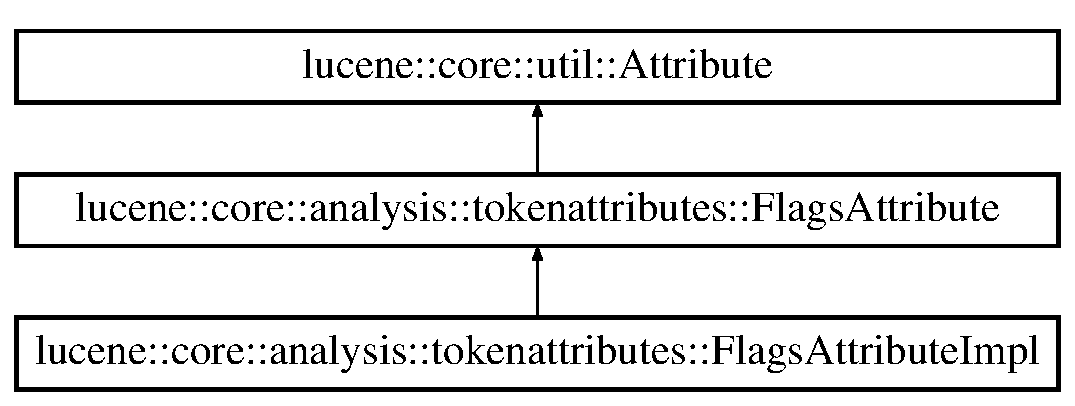
\includegraphics[height=3.000000cm]{classlucene_1_1core_1_1analysis_1_1tokenattributes_1_1FlagsAttribute}
\end{center}
\end{figure}
\subsection*{Public Member Functions}
\begin{DoxyCompactItemize}
\item 
virtual \mbox{\hyperlink{classlucene_1_1core_1_1analysis_1_1tokenattributes_1_1FlagsAttribute_a09be2fa83a9b76607965596fc8264145}{$\sim$\+Flags\+Attribute}} ()
\item 
virtual int32\+\_\+t \mbox{\hyperlink{classlucene_1_1core_1_1analysis_1_1tokenattributes_1_1FlagsAttribute_af5e017643df32ab110aca8337c01006d}{Get\+Flags}} ()=0
\item 
virtual void \mbox{\hyperlink{classlucene_1_1core_1_1analysis_1_1tokenattributes_1_1FlagsAttribute_a95bb70b836e238f5134a0ba12bb01d3d}{Set\+Flags}} (int32\+\_\+t flags)=0
\end{DoxyCompactItemize}
\subsection*{Additional Inherited Members}


\subsection{Constructor \& Destructor Documentation}
\mbox{\Hypertarget{classlucene_1_1core_1_1analysis_1_1tokenattributes_1_1FlagsAttribute_a09be2fa83a9b76607965596fc8264145}\label{classlucene_1_1core_1_1analysis_1_1tokenattributes_1_1FlagsAttribute_a09be2fa83a9b76607965596fc8264145}} 
\index{lucene\+::core\+::analysis\+::tokenattributes\+::\+Flags\+Attribute@{lucene\+::core\+::analysis\+::tokenattributes\+::\+Flags\+Attribute}!````~Flags\+Attribute@{$\sim$\+Flags\+Attribute}}
\index{````~Flags\+Attribute@{$\sim$\+Flags\+Attribute}!lucene\+::core\+::analysis\+::tokenattributes\+::\+Flags\+Attribute@{lucene\+::core\+::analysis\+::tokenattributes\+::\+Flags\+Attribute}}
\subsubsection{\texorpdfstring{$\sim$\+Flags\+Attribute()}{~FlagsAttribute()}}
{\footnotesize\ttfamily virtual lucene\+::core\+::analysis\+::tokenattributes\+::\+Flags\+Attribute\+::$\sim$\+Flags\+Attribute (\begin{DoxyParamCaption}{ }\end{DoxyParamCaption})\hspace{0.3cm}{\ttfamily [inline]}, {\ttfamily [virtual]}}



\subsection{Member Function Documentation}
\mbox{\Hypertarget{classlucene_1_1core_1_1analysis_1_1tokenattributes_1_1FlagsAttribute_af5e017643df32ab110aca8337c01006d}\label{classlucene_1_1core_1_1analysis_1_1tokenattributes_1_1FlagsAttribute_af5e017643df32ab110aca8337c01006d}} 
\index{lucene\+::core\+::analysis\+::tokenattributes\+::\+Flags\+Attribute@{lucene\+::core\+::analysis\+::tokenattributes\+::\+Flags\+Attribute}!Get\+Flags@{Get\+Flags}}
\index{Get\+Flags@{Get\+Flags}!lucene\+::core\+::analysis\+::tokenattributes\+::\+Flags\+Attribute@{lucene\+::core\+::analysis\+::tokenattributes\+::\+Flags\+Attribute}}
\subsubsection{\texorpdfstring{Get\+Flags()}{GetFlags()}}
{\footnotesize\ttfamily virtual int32\+\_\+t lucene\+::core\+::analysis\+::tokenattributes\+::\+Flags\+Attribute\+::\+Get\+Flags (\begin{DoxyParamCaption}{ }\end{DoxyParamCaption})\hspace{0.3cm}{\ttfamily [pure virtual]}}



Implemented in \mbox{\hyperlink{classlucene_1_1core_1_1analysis_1_1tokenattributes_1_1FlagsAttributeImpl_aa3fb651752273e55f85419ef522eaa3e}{lucene\+::core\+::analysis\+::tokenattributes\+::\+Flags\+Attribute\+Impl}}.

\mbox{\Hypertarget{classlucene_1_1core_1_1analysis_1_1tokenattributes_1_1FlagsAttribute_a95bb70b836e238f5134a0ba12bb01d3d}\label{classlucene_1_1core_1_1analysis_1_1tokenattributes_1_1FlagsAttribute_a95bb70b836e238f5134a0ba12bb01d3d}} 
\index{lucene\+::core\+::analysis\+::tokenattributes\+::\+Flags\+Attribute@{lucene\+::core\+::analysis\+::tokenattributes\+::\+Flags\+Attribute}!Set\+Flags@{Set\+Flags}}
\index{Set\+Flags@{Set\+Flags}!lucene\+::core\+::analysis\+::tokenattributes\+::\+Flags\+Attribute@{lucene\+::core\+::analysis\+::tokenattributes\+::\+Flags\+Attribute}}
\subsubsection{\texorpdfstring{Set\+Flags()}{SetFlags()}}
{\footnotesize\ttfamily virtual void lucene\+::core\+::analysis\+::tokenattributes\+::\+Flags\+Attribute\+::\+Set\+Flags (\begin{DoxyParamCaption}\item[{int32\+\_\+t}]{flags }\end{DoxyParamCaption})\hspace{0.3cm}{\ttfamily [pure virtual]}}



Implemented in \mbox{\hyperlink{classlucene_1_1core_1_1analysis_1_1tokenattributes_1_1FlagsAttributeImpl_a89376727686a4e0cc86db2154dc2ea49}{lucene\+::core\+::analysis\+::tokenattributes\+::\+Flags\+Attribute\+Impl}}.



The documentation for this class was generated from the following file\+:\begin{DoxyCompactItemize}
\item 
Analysis/\mbox{\hyperlink{Analysis_2Attribute_8h}{Attribute.\+h}}\end{DoxyCompactItemize}

\hypertarget{classlucene_1_1core_1_1analysis_1_1tokenattributes_1_1FlagsAttributeImpl}{}\section{lucene\+:\+:core\+:\+:analysis\+:\+:tokenattributes\+:\+:Flags\+Attribute\+Impl Class Reference}
\label{classlucene_1_1core_1_1analysis_1_1tokenattributes_1_1FlagsAttributeImpl}\index{lucene\+::core\+::analysis\+::tokenattributes\+::\+Flags\+Attribute\+Impl@{lucene\+::core\+::analysis\+::tokenattributes\+::\+Flags\+Attribute\+Impl}}


{\ttfamily \#include $<$Attribute\+Impl.\+h$>$}

Inheritance diagram for lucene\+:\+:core\+:\+:analysis\+:\+:tokenattributes\+:\+:Flags\+Attribute\+Impl\+:\begin{figure}[H]
\begin{center}
\leavevmode
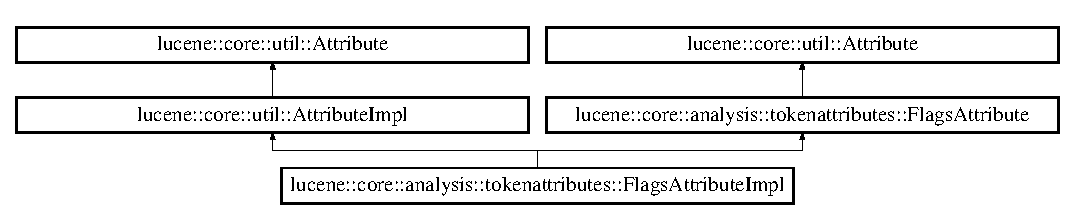
\includegraphics[height=2.507463cm]{classlucene_1_1core_1_1analysis_1_1tokenattributes_1_1FlagsAttributeImpl}
\end{center}
\end{figure}
\subsection*{Public Member Functions}
\begin{DoxyCompactItemize}
\item 
\mbox{\hyperlink{classlucene_1_1core_1_1analysis_1_1tokenattributes_1_1FlagsAttributeImpl_ac662a6d0887c9ffc42e3ef1ccc3f4256}{Flags\+Attribute\+Impl}} ()
\item 
\mbox{\hyperlink{classlucene_1_1core_1_1analysis_1_1tokenattributes_1_1FlagsAttributeImpl_ab9606f6a419551870e3c3233ff7a7954}{Flags\+Attribute\+Impl}} (\mbox{\hyperlink{ZlibCrc32_8h_a2c212835823e3c54a8ab6d95c652660e}{const}} \mbox{\hyperlink{classlucene_1_1core_1_1analysis_1_1tokenattributes_1_1FlagsAttributeImpl}{Flags\+Attribute\+Impl}} \&other)
\item 
virtual \mbox{\hyperlink{classlucene_1_1core_1_1analysis_1_1tokenattributes_1_1FlagsAttributeImpl_a643fd4820ca208193923bb08a10ac889}{$\sim$\+Flags\+Attribute\+Impl}} ()
\item 
int32\+\_\+t \mbox{\hyperlink{classlucene_1_1core_1_1analysis_1_1tokenattributes_1_1FlagsAttributeImpl_aa3fb651752273e55f85419ef522eaa3e}{Get\+Flags}} () override
\item 
void \mbox{\hyperlink{classlucene_1_1core_1_1analysis_1_1tokenattributes_1_1FlagsAttributeImpl_a89376727686a4e0cc86db2154dc2ea49}{Set\+Flags}} (\mbox{\hyperlink{ZlibCrc32_8h_a2c212835823e3c54a8ab6d95c652660e}{const}} int32\+\_\+t \mbox{\hyperlink{classlucene_1_1core_1_1analysis_1_1tokenattributes_1_1FlagsAttributeImpl_ac0a726a7b082414bcac0d9a5dc9ab4bb}{flags}}) override
\item 
void \mbox{\hyperlink{classlucene_1_1core_1_1analysis_1_1tokenattributes_1_1FlagsAttributeImpl_aa479cdc4474246af90f7d54ca64d3a48}{Reflect\+With}} (\mbox{\hyperlink{namespacelucene_1_1core_1_1util_a7dbb701adaed055f73fb95eec83da10a}{lucene\+::core\+::util\+::\+Attribute\+Reflector}} \&reflector) override
\item 
void \mbox{\hyperlink{classlucene_1_1core_1_1analysis_1_1tokenattributes_1_1FlagsAttributeImpl_a67ed39990f3f9eac90c91e880ad5cc31}{Clear}} () override
\item 
bool \mbox{\hyperlink{classlucene_1_1core_1_1analysis_1_1tokenattributes_1_1FlagsAttributeImpl_a93a0ee49b92c39e0a0d55c1f061f0ac2}{operator==}} (\mbox{\hyperlink{ZlibCrc32_8h_a2c212835823e3c54a8ab6d95c652660e}{const}} \mbox{\hyperlink{classlucene_1_1core_1_1analysis_1_1tokenattributes_1_1FlagsAttributeImpl}{Flags\+Attribute\+Impl}} \&other) \mbox{\hyperlink{ZlibCrc32_8h_a2c212835823e3c54a8ab6d95c652660e}{const}}
\item 
std\+::vector$<$ std\+::type\+\_\+index $>$ \mbox{\hyperlink{classlucene_1_1core_1_1analysis_1_1tokenattributes_1_1FlagsAttributeImpl_a3cdbd466551489b6f35ad51aa5ee2255}{Attributes}} () override
\item 
void \mbox{\hyperlink{classlucene_1_1core_1_1analysis_1_1tokenattributes_1_1FlagsAttributeImpl_a9c6a676eb175556a2eea6afaae666f8d}{Shallow\+Copy\+To}} (\mbox{\hyperlink{classlucene_1_1core_1_1util_1_1AttributeImpl}{lucene\+::core\+::util\+::\+Attribute\+Impl}} \&attr\+\_\+impl) override
\item 
\mbox{\hyperlink{classlucene_1_1core_1_1analysis_1_1tokenattributes_1_1FlagsAttributeImpl}{Flags\+Attribute\+Impl}} \& \mbox{\hyperlink{classlucene_1_1core_1_1analysis_1_1tokenattributes_1_1FlagsAttributeImpl_a41dfb20fafc327e7832e639695b453fa}{operator=}} (\mbox{\hyperlink{ZlibCrc32_8h_a2c212835823e3c54a8ab6d95c652660e}{const}} \mbox{\hyperlink{classlucene_1_1core_1_1util_1_1AttributeImpl}{lucene\+::core\+::util\+::\+Attribute\+Impl}} \&other)
\item 
\mbox{\hyperlink{classlucene_1_1core_1_1analysis_1_1tokenattributes_1_1FlagsAttributeImpl}{Flags\+Attribute\+Impl}} \& \mbox{\hyperlink{classlucene_1_1core_1_1analysis_1_1tokenattributes_1_1FlagsAttributeImpl_a32b03acbc1300103b4d96bd7e1a6ca2c}{operator=}} (\mbox{\hyperlink{ZlibCrc32_8h_a2c212835823e3c54a8ab6d95c652660e}{const}} \mbox{\hyperlink{classlucene_1_1core_1_1analysis_1_1tokenattributes_1_1FlagsAttributeImpl}{Flags\+Attribute\+Impl}} \&other)
\item 
\mbox{\hyperlink{classlucene_1_1core_1_1util_1_1AttributeImpl}{Attribute\+Impl}} $\ast$ \mbox{\hyperlink{classlucene_1_1core_1_1analysis_1_1tokenattributes_1_1FlagsAttributeImpl_aa920978da58dffbf7eb16bfa5e5f84c4}{Clone}} () override
\end{DoxyCompactItemize}
\subsection*{Private Attributes}
\begin{DoxyCompactItemize}
\item 
int32\+\_\+t \mbox{\hyperlink{classlucene_1_1core_1_1analysis_1_1tokenattributes_1_1FlagsAttributeImpl_ac0a726a7b082414bcac0d9a5dc9ab4bb}{flags}}
\end{DoxyCompactItemize}
\subsection*{Additional Inherited Members}


\subsection{Constructor \& Destructor Documentation}
\mbox{\Hypertarget{classlucene_1_1core_1_1analysis_1_1tokenattributes_1_1FlagsAttributeImpl_ac662a6d0887c9ffc42e3ef1ccc3f4256}\label{classlucene_1_1core_1_1analysis_1_1tokenattributes_1_1FlagsAttributeImpl_ac662a6d0887c9ffc42e3ef1ccc3f4256}} 
\index{lucene\+::core\+::analysis\+::tokenattributes\+::\+Flags\+Attribute\+Impl@{lucene\+::core\+::analysis\+::tokenattributes\+::\+Flags\+Attribute\+Impl}!Flags\+Attribute\+Impl@{Flags\+Attribute\+Impl}}
\index{Flags\+Attribute\+Impl@{Flags\+Attribute\+Impl}!lucene\+::core\+::analysis\+::tokenattributes\+::\+Flags\+Attribute\+Impl@{lucene\+::core\+::analysis\+::tokenattributes\+::\+Flags\+Attribute\+Impl}}
\subsubsection{\texorpdfstring{Flags\+Attribute\+Impl()}{FlagsAttributeImpl()}\hspace{0.1cm}{\footnotesize\ttfamily [1/2]}}
{\footnotesize\ttfamily Flags\+Attribute\+Impl\+::\+Flags\+Attribute\+Impl (\begin{DoxyParamCaption}{ }\end{DoxyParamCaption})}

\mbox{\hyperlink{classlucene_1_1core_1_1analysis_1_1tokenattributes_1_1FlagsAttributeImpl}{Flags\+Attribute\+Impl}} \mbox{\Hypertarget{classlucene_1_1core_1_1analysis_1_1tokenattributes_1_1FlagsAttributeImpl_ab9606f6a419551870e3c3233ff7a7954}\label{classlucene_1_1core_1_1analysis_1_1tokenattributes_1_1FlagsAttributeImpl_ab9606f6a419551870e3c3233ff7a7954}} 
\index{lucene\+::core\+::analysis\+::tokenattributes\+::\+Flags\+Attribute\+Impl@{lucene\+::core\+::analysis\+::tokenattributes\+::\+Flags\+Attribute\+Impl}!Flags\+Attribute\+Impl@{Flags\+Attribute\+Impl}}
\index{Flags\+Attribute\+Impl@{Flags\+Attribute\+Impl}!lucene\+::core\+::analysis\+::tokenattributes\+::\+Flags\+Attribute\+Impl@{lucene\+::core\+::analysis\+::tokenattributes\+::\+Flags\+Attribute\+Impl}}
\subsubsection{\texorpdfstring{Flags\+Attribute\+Impl()}{FlagsAttributeImpl()}\hspace{0.1cm}{\footnotesize\ttfamily [2/2]}}
{\footnotesize\ttfamily Flags\+Attribute\+Impl\+::\+Flags\+Attribute\+Impl (\begin{DoxyParamCaption}\item[{\mbox{\hyperlink{ZlibCrc32_8h_a2c212835823e3c54a8ab6d95c652660e}{const}} \mbox{\hyperlink{classlucene_1_1core_1_1analysis_1_1tokenattributes_1_1FlagsAttributeImpl}{Flags\+Attribute\+Impl}} \&}]{other }\end{DoxyParamCaption})}

\mbox{\Hypertarget{classlucene_1_1core_1_1analysis_1_1tokenattributes_1_1FlagsAttributeImpl_a643fd4820ca208193923bb08a10ac889}\label{classlucene_1_1core_1_1analysis_1_1tokenattributes_1_1FlagsAttributeImpl_a643fd4820ca208193923bb08a10ac889}} 
\index{lucene\+::core\+::analysis\+::tokenattributes\+::\+Flags\+Attribute\+Impl@{lucene\+::core\+::analysis\+::tokenattributes\+::\+Flags\+Attribute\+Impl}!````~Flags\+Attribute\+Impl@{$\sim$\+Flags\+Attribute\+Impl}}
\index{````~Flags\+Attribute\+Impl@{$\sim$\+Flags\+Attribute\+Impl}!lucene\+::core\+::analysis\+::tokenattributes\+::\+Flags\+Attribute\+Impl@{lucene\+::core\+::analysis\+::tokenattributes\+::\+Flags\+Attribute\+Impl}}
\subsubsection{\texorpdfstring{$\sim$\+Flags\+Attribute\+Impl()}{~FlagsAttributeImpl()}}
{\footnotesize\ttfamily Flags\+Attribute\+Impl\+::$\sim$\+Flags\+Attribute\+Impl (\begin{DoxyParamCaption}{ }\end{DoxyParamCaption})\hspace{0.3cm}{\ttfamily [virtual]}}



\subsection{Member Function Documentation}
\mbox{\Hypertarget{classlucene_1_1core_1_1analysis_1_1tokenattributes_1_1FlagsAttributeImpl_a3cdbd466551489b6f35ad51aa5ee2255}\label{classlucene_1_1core_1_1analysis_1_1tokenattributes_1_1FlagsAttributeImpl_a3cdbd466551489b6f35ad51aa5ee2255}} 
\index{lucene\+::core\+::analysis\+::tokenattributes\+::\+Flags\+Attribute\+Impl@{lucene\+::core\+::analysis\+::tokenattributes\+::\+Flags\+Attribute\+Impl}!Attributes@{Attributes}}
\index{Attributes@{Attributes}!lucene\+::core\+::analysis\+::tokenattributes\+::\+Flags\+Attribute\+Impl@{lucene\+::core\+::analysis\+::tokenattributes\+::\+Flags\+Attribute\+Impl}}
\subsubsection{\texorpdfstring{Attributes()}{Attributes()}}
{\footnotesize\ttfamily std\+::vector$<$ std\+::type\+\_\+index $>$ Flags\+Attribute\+Impl\+::\+Attributes (\begin{DoxyParamCaption}{ }\end{DoxyParamCaption})\hspace{0.3cm}{\ttfamily [override]}, {\ttfamily [virtual]}}



Implements \mbox{\hyperlink{classlucene_1_1core_1_1util_1_1AttributeImpl_ac0631e6a7a11044883bc97447716d7cc}{lucene\+::core\+::util\+::\+Attribute\+Impl}}.

\mbox{\Hypertarget{classlucene_1_1core_1_1analysis_1_1tokenattributes_1_1FlagsAttributeImpl_a67ed39990f3f9eac90c91e880ad5cc31}\label{classlucene_1_1core_1_1analysis_1_1tokenattributes_1_1FlagsAttributeImpl_a67ed39990f3f9eac90c91e880ad5cc31}} 
\index{lucene\+::core\+::analysis\+::tokenattributes\+::\+Flags\+Attribute\+Impl@{lucene\+::core\+::analysis\+::tokenattributes\+::\+Flags\+Attribute\+Impl}!Clear@{Clear}}
\index{Clear@{Clear}!lucene\+::core\+::analysis\+::tokenattributes\+::\+Flags\+Attribute\+Impl@{lucene\+::core\+::analysis\+::tokenattributes\+::\+Flags\+Attribute\+Impl}}
\subsubsection{\texorpdfstring{Clear()}{Clear()}}
{\footnotesize\ttfamily void Flags\+Attribute\+Impl\+::\+Clear (\begin{DoxyParamCaption}{ }\end{DoxyParamCaption})\hspace{0.3cm}{\ttfamily [override]}, {\ttfamily [virtual]}}



Implements \mbox{\hyperlink{classlucene_1_1core_1_1util_1_1AttributeImpl_a04897a00a902f7a345dd44bbc4b482a8}{lucene\+::core\+::util\+::\+Attribute\+Impl}}.

\mbox{\Hypertarget{classlucene_1_1core_1_1analysis_1_1tokenattributes_1_1FlagsAttributeImpl_aa920978da58dffbf7eb16bfa5e5f84c4}\label{classlucene_1_1core_1_1analysis_1_1tokenattributes_1_1FlagsAttributeImpl_aa920978da58dffbf7eb16bfa5e5f84c4}} 
\index{lucene\+::core\+::analysis\+::tokenattributes\+::\+Flags\+Attribute\+Impl@{lucene\+::core\+::analysis\+::tokenattributes\+::\+Flags\+Attribute\+Impl}!Clone@{Clone}}
\index{Clone@{Clone}!lucene\+::core\+::analysis\+::tokenattributes\+::\+Flags\+Attribute\+Impl@{lucene\+::core\+::analysis\+::tokenattributes\+::\+Flags\+Attribute\+Impl}}
\subsubsection{\texorpdfstring{Clone()}{Clone()}}
{\footnotesize\ttfamily \mbox{\hyperlink{classlucene_1_1core_1_1util_1_1AttributeImpl}{Attribute\+Impl}} $\ast$ Flags\+Attribute\+Impl\+::\+Clone (\begin{DoxyParamCaption}{ }\end{DoxyParamCaption})\hspace{0.3cm}{\ttfamily [override]}, {\ttfamily [virtual]}}



Implements \mbox{\hyperlink{classlucene_1_1core_1_1util_1_1AttributeImpl_a135318ad4c7c17b3d85e625e32fb42cd}{lucene\+::core\+::util\+::\+Attribute\+Impl}}.

\mbox{\Hypertarget{classlucene_1_1core_1_1analysis_1_1tokenattributes_1_1FlagsAttributeImpl_aa3fb651752273e55f85419ef522eaa3e}\label{classlucene_1_1core_1_1analysis_1_1tokenattributes_1_1FlagsAttributeImpl_aa3fb651752273e55f85419ef522eaa3e}} 
\index{lucene\+::core\+::analysis\+::tokenattributes\+::\+Flags\+Attribute\+Impl@{lucene\+::core\+::analysis\+::tokenattributes\+::\+Flags\+Attribute\+Impl}!Get\+Flags@{Get\+Flags}}
\index{Get\+Flags@{Get\+Flags}!lucene\+::core\+::analysis\+::tokenattributes\+::\+Flags\+Attribute\+Impl@{lucene\+::core\+::analysis\+::tokenattributes\+::\+Flags\+Attribute\+Impl}}
\subsubsection{\texorpdfstring{Get\+Flags()}{GetFlags()}}
{\footnotesize\ttfamily int32\+\_\+t Flags\+Attribute\+Impl\+::\+Get\+Flags (\begin{DoxyParamCaption}{ }\end{DoxyParamCaption})\hspace{0.3cm}{\ttfamily [override]}, {\ttfamily [virtual]}}



Implements \mbox{\hyperlink{classlucene_1_1core_1_1analysis_1_1tokenattributes_1_1FlagsAttribute_af5e017643df32ab110aca8337c01006d}{lucene\+::core\+::analysis\+::tokenattributes\+::\+Flags\+Attribute}}.

\mbox{\Hypertarget{classlucene_1_1core_1_1analysis_1_1tokenattributes_1_1FlagsAttributeImpl_a41dfb20fafc327e7832e639695b453fa}\label{classlucene_1_1core_1_1analysis_1_1tokenattributes_1_1FlagsAttributeImpl_a41dfb20fafc327e7832e639695b453fa}} 
\index{lucene\+::core\+::analysis\+::tokenattributes\+::\+Flags\+Attribute\+Impl@{lucene\+::core\+::analysis\+::tokenattributes\+::\+Flags\+Attribute\+Impl}!operator=@{operator=}}
\index{operator=@{operator=}!lucene\+::core\+::analysis\+::tokenattributes\+::\+Flags\+Attribute\+Impl@{lucene\+::core\+::analysis\+::tokenattributes\+::\+Flags\+Attribute\+Impl}}
\subsubsection{\texorpdfstring{operator=()}{operator=()}\hspace{0.1cm}{\footnotesize\ttfamily [1/2]}}
{\footnotesize\ttfamily \mbox{\hyperlink{classlucene_1_1core_1_1analysis_1_1tokenattributes_1_1FlagsAttributeImpl}{Flags\+Attribute\+Impl}} \& Flags\+Attribute\+Impl\+::operator= (\begin{DoxyParamCaption}\item[{\mbox{\hyperlink{ZlibCrc32_8h_a2c212835823e3c54a8ab6d95c652660e}{const}} \mbox{\hyperlink{classlucene_1_1core_1_1util_1_1AttributeImpl}{lucene\+::core\+::util\+::\+Attribute\+Impl}} \&}]{other }\end{DoxyParamCaption})\hspace{0.3cm}{\ttfamily [virtual]}}



Implements \mbox{\hyperlink{classlucene_1_1core_1_1util_1_1AttributeImpl_ab032e399d03ce2f58c76881cf2b92325}{lucene\+::core\+::util\+::\+Attribute\+Impl}}.

\mbox{\Hypertarget{classlucene_1_1core_1_1analysis_1_1tokenattributes_1_1FlagsAttributeImpl_a32b03acbc1300103b4d96bd7e1a6ca2c}\label{classlucene_1_1core_1_1analysis_1_1tokenattributes_1_1FlagsAttributeImpl_a32b03acbc1300103b4d96bd7e1a6ca2c}} 
\index{lucene\+::core\+::analysis\+::tokenattributes\+::\+Flags\+Attribute\+Impl@{lucene\+::core\+::analysis\+::tokenattributes\+::\+Flags\+Attribute\+Impl}!operator=@{operator=}}
\index{operator=@{operator=}!lucene\+::core\+::analysis\+::tokenattributes\+::\+Flags\+Attribute\+Impl@{lucene\+::core\+::analysis\+::tokenattributes\+::\+Flags\+Attribute\+Impl}}
\subsubsection{\texorpdfstring{operator=()}{operator=()}\hspace{0.1cm}{\footnotesize\ttfamily [2/2]}}
{\footnotesize\ttfamily \mbox{\hyperlink{classlucene_1_1core_1_1analysis_1_1tokenattributes_1_1FlagsAttributeImpl}{Flags\+Attribute\+Impl}} \& Flags\+Attribute\+Impl\+::operator= (\begin{DoxyParamCaption}\item[{\mbox{\hyperlink{ZlibCrc32_8h_a2c212835823e3c54a8ab6d95c652660e}{const}} \mbox{\hyperlink{classlucene_1_1core_1_1analysis_1_1tokenattributes_1_1FlagsAttributeImpl}{Flags\+Attribute\+Impl}} \&}]{other }\end{DoxyParamCaption})}

\mbox{\Hypertarget{classlucene_1_1core_1_1analysis_1_1tokenattributes_1_1FlagsAttributeImpl_a93a0ee49b92c39e0a0d55c1f061f0ac2}\label{classlucene_1_1core_1_1analysis_1_1tokenattributes_1_1FlagsAttributeImpl_a93a0ee49b92c39e0a0d55c1f061f0ac2}} 
\index{lucene\+::core\+::analysis\+::tokenattributes\+::\+Flags\+Attribute\+Impl@{lucene\+::core\+::analysis\+::tokenattributes\+::\+Flags\+Attribute\+Impl}!operator==@{operator==}}
\index{operator==@{operator==}!lucene\+::core\+::analysis\+::tokenattributes\+::\+Flags\+Attribute\+Impl@{lucene\+::core\+::analysis\+::tokenattributes\+::\+Flags\+Attribute\+Impl}}
\subsubsection{\texorpdfstring{operator==()}{operator==()}}
{\footnotesize\ttfamily bool Flags\+Attribute\+Impl\+::operator== (\begin{DoxyParamCaption}\item[{\mbox{\hyperlink{ZlibCrc32_8h_a2c212835823e3c54a8ab6d95c652660e}{const}} \mbox{\hyperlink{classlucene_1_1core_1_1analysis_1_1tokenattributes_1_1FlagsAttributeImpl}{Flags\+Attribute\+Impl}} \&}]{other }\end{DoxyParamCaption}) const}

\mbox{\Hypertarget{classlucene_1_1core_1_1analysis_1_1tokenattributes_1_1FlagsAttributeImpl_aa479cdc4474246af90f7d54ca64d3a48}\label{classlucene_1_1core_1_1analysis_1_1tokenattributes_1_1FlagsAttributeImpl_aa479cdc4474246af90f7d54ca64d3a48}} 
\index{lucene\+::core\+::analysis\+::tokenattributes\+::\+Flags\+Attribute\+Impl@{lucene\+::core\+::analysis\+::tokenattributes\+::\+Flags\+Attribute\+Impl}!Reflect\+With@{Reflect\+With}}
\index{Reflect\+With@{Reflect\+With}!lucene\+::core\+::analysis\+::tokenattributes\+::\+Flags\+Attribute\+Impl@{lucene\+::core\+::analysis\+::tokenattributes\+::\+Flags\+Attribute\+Impl}}
\subsubsection{\texorpdfstring{Reflect\+With()}{ReflectWith()}}
{\footnotesize\ttfamily void Flags\+Attribute\+Impl\+::\+Reflect\+With (\begin{DoxyParamCaption}\item[{\mbox{\hyperlink{namespacelucene_1_1core_1_1util_a7dbb701adaed055f73fb95eec83da10a}{lucene\+::core\+::util\+::\+Attribute\+Reflector}} \&}]{reflector }\end{DoxyParamCaption})\hspace{0.3cm}{\ttfamily [override]}, {\ttfamily [virtual]}}



Implements \mbox{\hyperlink{classlucene_1_1core_1_1util_1_1AttributeImpl_a84d34275fb1ed67ac36fad7ff6388096}{lucene\+::core\+::util\+::\+Attribute\+Impl}}.

\mbox{\Hypertarget{classlucene_1_1core_1_1analysis_1_1tokenattributes_1_1FlagsAttributeImpl_a89376727686a4e0cc86db2154dc2ea49}\label{classlucene_1_1core_1_1analysis_1_1tokenattributes_1_1FlagsAttributeImpl_a89376727686a4e0cc86db2154dc2ea49}} 
\index{lucene\+::core\+::analysis\+::tokenattributes\+::\+Flags\+Attribute\+Impl@{lucene\+::core\+::analysis\+::tokenattributes\+::\+Flags\+Attribute\+Impl}!Set\+Flags@{Set\+Flags}}
\index{Set\+Flags@{Set\+Flags}!lucene\+::core\+::analysis\+::tokenattributes\+::\+Flags\+Attribute\+Impl@{lucene\+::core\+::analysis\+::tokenattributes\+::\+Flags\+Attribute\+Impl}}
\subsubsection{\texorpdfstring{Set\+Flags()}{SetFlags()}}
{\footnotesize\ttfamily void Flags\+Attribute\+Impl\+::\+Set\+Flags (\begin{DoxyParamCaption}\item[{\mbox{\hyperlink{ZlibCrc32_8h_a2c212835823e3c54a8ab6d95c652660e}{const}} int32\+\_\+t}]{flags }\end{DoxyParamCaption})\hspace{0.3cm}{\ttfamily [override]}, {\ttfamily [virtual]}}



Implements \mbox{\hyperlink{classlucene_1_1core_1_1analysis_1_1tokenattributes_1_1FlagsAttribute_a95bb70b836e238f5134a0ba12bb01d3d}{lucene\+::core\+::analysis\+::tokenattributes\+::\+Flags\+Attribute}}.

\mbox{\Hypertarget{classlucene_1_1core_1_1analysis_1_1tokenattributes_1_1FlagsAttributeImpl_a9c6a676eb175556a2eea6afaae666f8d}\label{classlucene_1_1core_1_1analysis_1_1tokenattributes_1_1FlagsAttributeImpl_a9c6a676eb175556a2eea6afaae666f8d}} 
\index{lucene\+::core\+::analysis\+::tokenattributes\+::\+Flags\+Attribute\+Impl@{lucene\+::core\+::analysis\+::tokenattributes\+::\+Flags\+Attribute\+Impl}!Shallow\+Copy\+To@{Shallow\+Copy\+To}}
\index{Shallow\+Copy\+To@{Shallow\+Copy\+To}!lucene\+::core\+::analysis\+::tokenattributes\+::\+Flags\+Attribute\+Impl@{lucene\+::core\+::analysis\+::tokenattributes\+::\+Flags\+Attribute\+Impl}}
\subsubsection{\texorpdfstring{Shallow\+Copy\+To()}{ShallowCopyTo()}}
{\footnotesize\ttfamily void Flags\+Attribute\+Impl\+::\+Shallow\+Copy\+To (\begin{DoxyParamCaption}\item[{\mbox{\hyperlink{classlucene_1_1core_1_1util_1_1AttributeImpl}{lucene\+::core\+::util\+::\+Attribute\+Impl}} \&}]{attr\+\_\+impl }\end{DoxyParamCaption})\hspace{0.3cm}{\ttfamily [override]}, {\ttfamily [virtual]}}



Implements \mbox{\hyperlink{classlucene_1_1core_1_1util_1_1AttributeImpl_a010e8937832f53139c8fe42757476895}{lucene\+::core\+::util\+::\+Attribute\+Impl}}.



\subsection{Member Data Documentation}
\mbox{\Hypertarget{classlucene_1_1core_1_1analysis_1_1tokenattributes_1_1FlagsAttributeImpl_ac0a726a7b082414bcac0d9a5dc9ab4bb}\label{classlucene_1_1core_1_1analysis_1_1tokenattributes_1_1FlagsAttributeImpl_ac0a726a7b082414bcac0d9a5dc9ab4bb}} 
\index{lucene\+::core\+::analysis\+::tokenattributes\+::\+Flags\+Attribute\+Impl@{lucene\+::core\+::analysis\+::tokenattributes\+::\+Flags\+Attribute\+Impl}!flags@{flags}}
\index{flags@{flags}!lucene\+::core\+::analysis\+::tokenattributes\+::\+Flags\+Attribute\+Impl@{lucene\+::core\+::analysis\+::tokenattributes\+::\+Flags\+Attribute\+Impl}}
\subsubsection{\texorpdfstring{flags}{flags}}
{\footnotesize\ttfamily int32\+\_\+t lucene\+::core\+::analysis\+::tokenattributes\+::\+Flags\+Attribute\+Impl\+::flags\hspace{0.3cm}{\ttfamily [private]}}



The documentation for this class was generated from the following files\+:\begin{DoxyCompactItemize}
\item 
Analysis/\mbox{\hyperlink{AttributeImpl_8h}{Attribute\+Impl.\+h}}\item 
Analysis/\mbox{\hyperlink{AttributeImpl_8cpp}{Attribute\+Impl.\+cpp}}\end{DoxyCompactItemize}

\hypertarget{classlucene_1_1core_1_1analysis_1_1GlobalReuseStrategy}{}\section{lucene\+:\+:core\+:\+:analysis\+:\+:Global\+Reuse\+Strategy Class Reference}
\label{classlucene_1_1core_1_1analysis_1_1GlobalReuseStrategy}\index{lucene\+::core\+::analysis\+::\+Global\+Reuse\+Strategy@{lucene\+::core\+::analysis\+::\+Global\+Reuse\+Strategy}}


{\ttfamily \#include $<$Analyzer.\+h$>$}

Inheritance diagram for lucene\+:\+:core\+:\+:analysis\+:\+:Global\+Reuse\+Strategy\+:\begin{figure}[H]
\begin{center}
\leavevmode
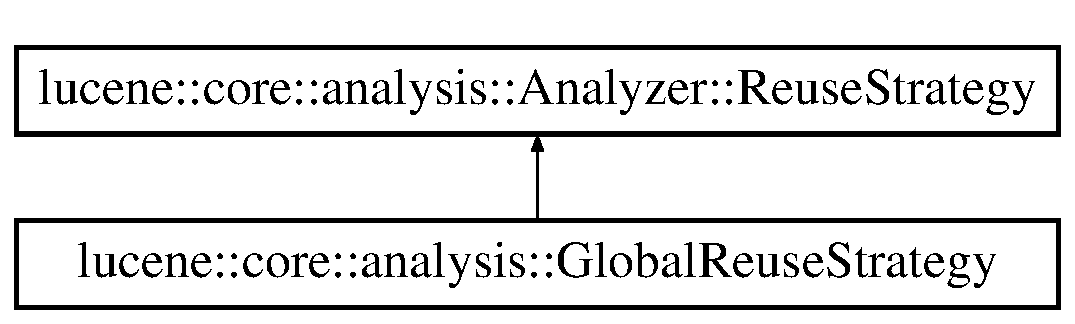
\includegraphics[height=2.000000cm]{classlucene_1_1core_1_1analysis_1_1GlobalReuseStrategy}
\end{center}
\end{figure}
\subsection*{Public Member Functions}
\begin{DoxyCompactItemize}
\item 
\mbox{\hyperlink{classlucene_1_1core_1_1analysis_1_1GlobalReuseStrategy_ac91815e66d775fd48aad17fb5a78d266}{Global\+Reuse\+Strategy}} ()
\item 
virtual \mbox{\hyperlink{classlucene_1_1core_1_1analysis_1_1GlobalReuseStrategy_a536f4c3459f19db2a356e6cedb575c1a}{$\sim$\+Global\+Reuse\+Strategy}} ()
\item 
\mbox{\hyperlink{classlucene_1_1core_1_1analysis_1_1TokenStreamComponents}{Token\+Stream\+Components}} $\ast$ \mbox{\hyperlink{classlucene_1_1core_1_1analysis_1_1GlobalReuseStrategy_a79b31d1f8bf9bec685377f6dbff3c5ba}{Get\+Reusable\+Components}} (\mbox{\hyperlink{classlucene_1_1core_1_1analysis_1_1Analyzer}{Analyzer}} \&analyzer, \mbox{\hyperlink{ZlibCrc32_8h_a2c212835823e3c54a8ab6d95c652660e}{const}} std\+::string \&field\+\_\+name) override
\item 
void \mbox{\hyperlink{classlucene_1_1core_1_1analysis_1_1GlobalReuseStrategy_a168d01df604559cb787781ad0ab7d7c2}{Set\+Reusable\+Components}} (\mbox{\hyperlink{classlucene_1_1core_1_1analysis_1_1Analyzer}{Analyzer}} \&analyzer, \mbox{\hyperlink{ZlibCrc32_8h_a2c212835823e3c54a8ab6d95c652660e}{const}} std\+::string \&field\+\_\+name, \mbox{\hyperlink{classlucene_1_1core_1_1analysis_1_1TokenStreamComponents}{Token\+Stream\+Components}} $\ast$components) override
\end{DoxyCompactItemize}
\subsection*{Private Attributes}
\begin{DoxyCompactItemize}
\item 
\mbox{\hyperlink{classlucene_1_1core_1_1util_1_1CloseableThreadLocal}{lucene\+::core\+::util\+::\+Closeable\+Thread\+Local}}$<$ \mbox{\hyperlink{classlucene_1_1core_1_1analysis_1_1GlobalReuseStrategy}{Global\+Reuse\+Strategy}}, std\+::unique\+\_\+ptr$<$ \mbox{\hyperlink{classlucene_1_1core_1_1analysis_1_1TokenStreamComponents}{Token\+Stream\+Components}} $>$ $>$ \mbox{\hyperlink{classlucene_1_1core_1_1analysis_1_1GlobalReuseStrategy_aa46c26280248f8f15c138db30d2a5991}{stored\+\_\+value}}
\end{DoxyCompactItemize}


\subsection{Constructor \& Destructor Documentation}
\mbox{\Hypertarget{classlucene_1_1core_1_1analysis_1_1GlobalReuseStrategy_ac91815e66d775fd48aad17fb5a78d266}\label{classlucene_1_1core_1_1analysis_1_1GlobalReuseStrategy_ac91815e66d775fd48aad17fb5a78d266}} 
\index{lucene\+::core\+::analysis\+::\+Global\+Reuse\+Strategy@{lucene\+::core\+::analysis\+::\+Global\+Reuse\+Strategy}!Global\+Reuse\+Strategy@{Global\+Reuse\+Strategy}}
\index{Global\+Reuse\+Strategy@{Global\+Reuse\+Strategy}!lucene\+::core\+::analysis\+::\+Global\+Reuse\+Strategy@{lucene\+::core\+::analysis\+::\+Global\+Reuse\+Strategy}}
\subsubsection{\texorpdfstring{Global\+Reuse\+Strategy()}{GlobalReuseStrategy()}}
{\footnotesize\ttfamily Global\+Reuse\+Strategy\+::\+Global\+Reuse\+Strategy (\begin{DoxyParamCaption}{ }\end{DoxyParamCaption})}

\mbox{\hyperlink{classlucene_1_1core_1_1analysis_1_1GlobalReuseStrategy}{Global\+Reuse\+Strategy}} \mbox{\Hypertarget{classlucene_1_1core_1_1analysis_1_1GlobalReuseStrategy_a536f4c3459f19db2a356e6cedb575c1a}\label{classlucene_1_1core_1_1analysis_1_1GlobalReuseStrategy_a536f4c3459f19db2a356e6cedb575c1a}} 
\index{lucene\+::core\+::analysis\+::\+Global\+Reuse\+Strategy@{lucene\+::core\+::analysis\+::\+Global\+Reuse\+Strategy}!````~Global\+Reuse\+Strategy@{$\sim$\+Global\+Reuse\+Strategy}}
\index{````~Global\+Reuse\+Strategy@{$\sim$\+Global\+Reuse\+Strategy}!lucene\+::core\+::analysis\+::\+Global\+Reuse\+Strategy@{lucene\+::core\+::analysis\+::\+Global\+Reuse\+Strategy}}
\subsubsection{\texorpdfstring{$\sim$\+Global\+Reuse\+Strategy()}{~GlobalReuseStrategy()}}
{\footnotesize\ttfamily Global\+Reuse\+Strategy\+::$\sim$\+Global\+Reuse\+Strategy (\begin{DoxyParamCaption}{ }\end{DoxyParamCaption})\hspace{0.3cm}{\ttfamily [virtual]}}



\subsection{Member Function Documentation}
\mbox{\Hypertarget{classlucene_1_1core_1_1analysis_1_1GlobalReuseStrategy_a79b31d1f8bf9bec685377f6dbff3c5ba}\label{classlucene_1_1core_1_1analysis_1_1GlobalReuseStrategy_a79b31d1f8bf9bec685377f6dbff3c5ba}} 
\index{lucene\+::core\+::analysis\+::\+Global\+Reuse\+Strategy@{lucene\+::core\+::analysis\+::\+Global\+Reuse\+Strategy}!Get\+Reusable\+Components@{Get\+Reusable\+Components}}
\index{Get\+Reusable\+Components@{Get\+Reusable\+Components}!lucene\+::core\+::analysis\+::\+Global\+Reuse\+Strategy@{lucene\+::core\+::analysis\+::\+Global\+Reuse\+Strategy}}
\subsubsection{\texorpdfstring{Get\+Reusable\+Components()}{GetReusableComponents()}}
{\footnotesize\ttfamily \mbox{\hyperlink{classlucene_1_1core_1_1analysis_1_1TokenStreamComponents}{Token\+Stream\+Components}} $\ast$ Global\+Reuse\+Strategy\+::\+Get\+Reusable\+Components (\begin{DoxyParamCaption}\item[{\mbox{\hyperlink{classlucene_1_1core_1_1analysis_1_1Analyzer}{Analyzer}} \&}]{analyzer,  }\item[{\mbox{\hyperlink{ZlibCrc32_8h_a2c212835823e3c54a8ab6d95c652660e}{const}} std\+::string \&}]{field\+\_\+name }\end{DoxyParamCaption})\hspace{0.3cm}{\ttfamily [override]}, {\ttfamily [virtual]}}



Implements \mbox{\hyperlink{classlucene_1_1core_1_1analysis_1_1Analyzer_1_1ReuseStrategy_ab180767950f392037e8ddf78c2f11f95}{lucene\+::core\+::analysis\+::\+Analyzer\+::\+Reuse\+Strategy}}.

\mbox{\Hypertarget{classlucene_1_1core_1_1analysis_1_1GlobalReuseStrategy_a168d01df604559cb787781ad0ab7d7c2}\label{classlucene_1_1core_1_1analysis_1_1GlobalReuseStrategy_a168d01df604559cb787781ad0ab7d7c2}} 
\index{lucene\+::core\+::analysis\+::\+Global\+Reuse\+Strategy@{lucene\+::core\+::analysis\+::\+Global\+Reuse\+Strategy}!Set\+Reusable\+Components@{Set\+Reusable\+Components}}
\index{Set\+Reusable\+Components@{Set\+Reusable\+Components}!lucene\+::core\+::analysis\+::\+Global\+Reuse\+Strategy@{lucene\+::core\+::analysis\+::\+Global\+Reuse\+Strategy}}
\subsubsection{\texorpdfstring{Set\+Reusable\+Components()}{SetReusableComponents()}}
{\footnotesize\ttfamily void Global\+Reuse\+Strategy\+::\+Set\+Reusable\+Components (\begin{DoxyParamCaption}\item[{\mbox{\hyperlink{classlucene_1_1core_1_1analysis_1_1Analyzer}{Analyzer}} \&}]{analyzer,  }\item[{\mbox{\hyperlink{ZlibCrc32_8h_a2c212835823e3c54a8ab6d95c652660e}{const}} std\+::string \&}]{field\+\_\+name,  }\item[{\mbox{\hyperlink{classlucene_1_1core_1_1analysis_1_1TokenStreamComponents}{Token\+Stream\+Components}} $\ast$}]{components }\end{DoxyParamCaption})\hspace{0.3cm}{\ttfamily [override]}, {\ttfamily [virtual]}}



Implements \mbox{\hyperlink{classlucene_1_1core_1_1analysis_1_1Analyzer_1_1ReuseStrategy_a78a1328d5564e78e2168169b73094b23}{lucene\+::core\+::analysis\+::\+Analyzer\+::\+Reuse\+Strategy}}.



\subsection{Member Data Documentation}
\mbox{\Hypertarget{classlucene_1_1core_1_1analysis_1_1GlobalReuseStrategy_aa46c26280248f8f15c138db30d2a5991}\label{classlucene_1_1core_1_1analysis_1_1GlobalReuseStrategy_aa46c26280248f8f15c138db30d2a5991}} 
\index{lucene\+::core\+::analysis\+::\+Global\+Reuse\+Strategy@{lucene\+::core\+::analysis\+::\+Global\+Reuse\+Strategy}!stored\+\_\+value@{stored\+\_\+value}}
\index{stored\+\_\+value@{stored\+\_\+value}!lucene\+::core\+::analysis\+::\+Global\+Reuse\+Strategy@{lucene\+::core\+::analysis\+::\+Global\+Reuse\+Strategy}}
\subsubsection{\texorpdfstring{stored\+\_\+value}{stored\_value}}
{\footnotesize\ttfamily \mbox{\hyperlink{classlucene_1_1core_1_1util_1_1CloseableThreadLocal}{lucene\+::core\+::util\+::\+Closeable\+Thread\+Local}}$<$\mbox{\hyperlink{classlucene_1_1core_1_1analysis_1_1GlobalReuseStrategy}{Global\+Reuse\+Strategy}}, std\+::unique\+\_\+ptr$<$ \mbox{\hyperlink{classlucene_1_1core_1_1analysis_1_1TokenStreamComponents}{Token\+Stream\+Components}}$>$ $>$ lucene\+::core\+::analysis\+::\+Global\+Reuse\+Strategy\+::stored\+\_\+value\hspace{0.3cm}{\ttfamily [private]}}



The documentation for this class was generated from the following files\+:\begin{DoxyCompactItemize}
\item 
Analysis/\mbox{\hyperlink{Analyzer_8h}{Analyzer.\+h}}\item 
Analysis/\mbox{\hyperlink{Analyzer_8cpp}{Analyzer.\+cpp}}\end{DoxyCompactItemize}

\hypertarget{classHateThreeWordsTokenFilter}{}\section{Hate\+Three\+Words\+Token\+Filter Class Reference}
\label{classHateThreeWordsTokenFilter}\index{Hate\+Three\+Words\+Token\+Filter@{Hate\+Three\+Words\+Token\+Filter}}
Inheritance diagram for Hate\+Three\+Words\+Token\+Filter\+:\begin{figure}[H]
\begin{center}
\leavevmode
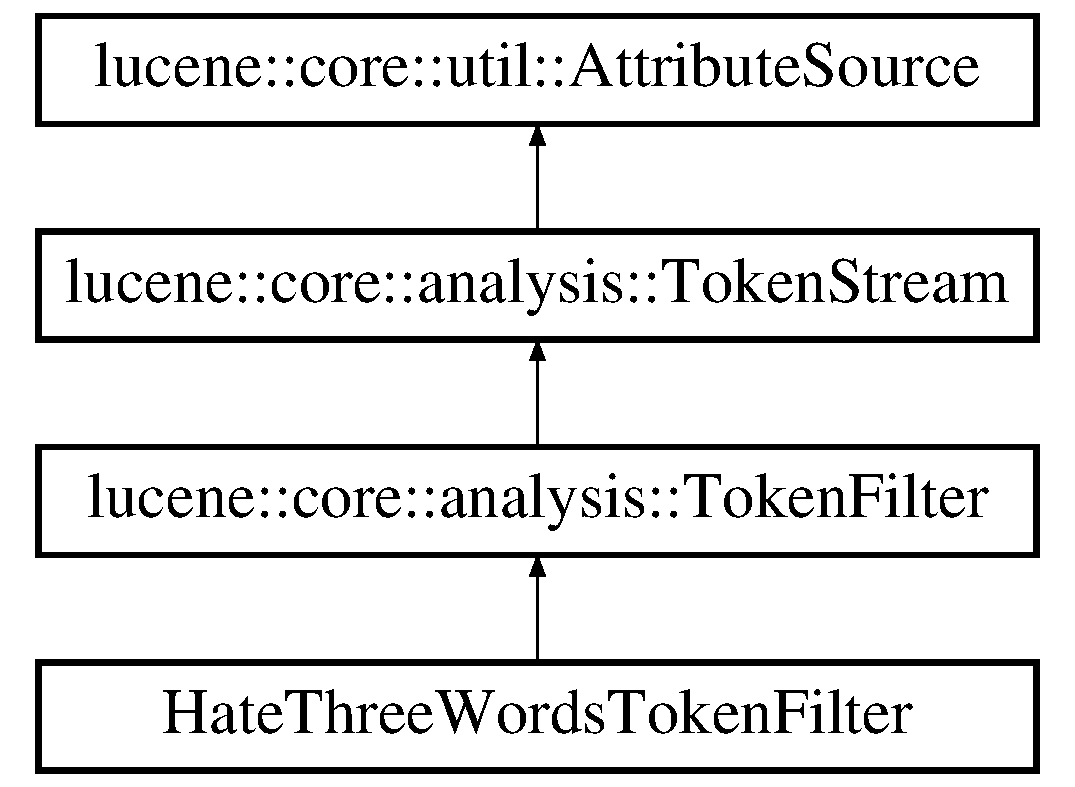
\includegraphics[height=4.000000cm]{classHateThreeWordsTokenFilter}
\end{center}
\end{figure}
\subsection*{Public Member Functions}
\begin{DoxyCompactItemize}
\item 
\mbox{\hyperlink{classHateThreeWordsTokenFilter_a8be911badf576176b0168d86e33467c2}{Hate\+Three\+Words\+Token\+Filter}} (\mbox{\hyperlink{classlucene_1_1core_1_1analysis_1_1TokenStream}{Token\+Stream}} $\ast$in)
\item 
bool \mbox{\hyperlink{classHateThreeWordsTokenFilter_ad843fcf23da10776311702c619c02560}{Increment\+Token}} () override
\end{DoxyCompactItemize}
\subsection*{Public Attributes}
\begin{DoxyCompactItemize}
\item 
std\+::shared\+\_\+ptr$<$ \mbox{\hyperlink{classlucene_1_1core_1_1analysis_1_1tokenattributes_1_1CharTermAttribute}{Char\+Term\+Attribute}} $>$ \mbox{\hyperlink{classHateThreeWordsTokenFilter_a1474587e08f5c86b42c24badf44d7336}{term\+\_\+att}}
\item 
std\+::shared\+\_\+ptr$<$ \mbox{\hyperlink{classlucene_1_1core_1_1analysis_1_1tokenattributes_1_1OffsetAttribute}{Offset\+Attribute}} $>$ \mbox{\hyperlink{classHateThreeWordsTokenFilter_ab4f8e5cab969bbd844cff5ce59e78025}{offset\+\_\+att}}
\end{DoxyCompactItemize}
\subsection*{Additional Inherited Members}


\subsection{Constructor \& Destructor Documentation}
\mbox{\Hypertarget{classHateThreeWordsTokenFilter_a8be911badf576176b0168d86e33467c2}\label{classHateThreeWordsTokenFilter_a8be911badf576176b0168d86e33467c2}} 
\index{Hate\+Three\+Words\+Token\+Filter@{Hate\+Three\+Words\+Token\+Filter}!Hate\+Three\+Words\+Token\+Filter@{Hate\+Three\+Words\+Token\+Filter}}
\index{Hate\+Three\+Words\+Token\+Filter@{Hate\+Three\+Words\+Token\+Filter}!Hate\+Three\+Words\+Token\+Filter@{Hate\+Three\+Words\+Token\+Filter}}
\subsubsection{\texorpdfstring{Hate\+Three\+Words\+Token\+Filter()}{HateThreeWordsTokenFilter()}}
{\footnotesize\ttfamily Hate\+Three\+Words\+Token\+Filter\+::\+Hate\+Three\+Words\+Token\+Filter (\begin{DoxyParamCaption}\item[{\mbox{\hyperlink{classlucene_1_1core_1_1analysis_1_1TokenStream}{Token\+Stream}} $\ast$}]{in }\end{DoxyParamCaption})\hspace{0.3cm}{\ttfamily [inline]}, {\ttfamily [explicit]}}



\subsection{Member Function Documentation}
\mbox{\Hypertarget{classHateThreeWordsTokenFilter_ad843fcf23da10776311702c619c02560}\label{classHateThreeWordsTokenFilter_ad843fcf23da10776311702c619c02560}} 
\index{Hate\+Three\+Words\+Token\+Filter@{Hate\+Three\+Words\+Token\+Filter}!Increment\+Token@{Increment\+Token}}
\index{Increment\+Token@{Increment\+Token}!Hate\+Three\+Words\+Token\+Filter@{Hate\+Three\+Words\+Token\+Filter}}
\subsubsection{\texorpdfstring{Increment\+Token()}{IncrementToken()}}
{\footnotesize\ttfamily bool Hate\+Three\+Words\+Token\+Filter\+::\+Increment\+Token (\begin{DoxyParamCaption}{ }\end{DoxyParamCaption})\hspace{0.3cm}{\ttfamily [inline]}, {\ttfamily [override]}, {\ttfamily [virtual]}}



Implements \mbox{\hyperlink{classlucene_1_1core_1_1analysis_1_1TokenStream_a614d4ea24a354d6f4354b4941b5124e2}{lucene\+::core\+::analysis\+::\+Token\+Stream}}.



\subsection{Member Data Documentation}
\mbox{\Hypertarget{classHateThreeWordsTokenFilter_ab4f8e5cab969bbd844cff5ce59e78025}\label{classHateThreeWordsTokenFilter_ab4f8e5cab969bbd844cff5ce59e78025}} 
\index{Hate\+Three\+Words\+Token\+Filter@{Hate\+Three\+Words\+Token\+Filter}!offset\+\_\+att@{offset\+\_\+att}}
\index{offset\+\_\+att@{offset\+\_\+att}!Hate\+Three\+Words\+Token\+Filter@{Hate\+Three\+Words\+Token\+Filter}}
\subsubsection{\texorpdfstring{offset\+\_\+att}{offset\_att}}
{\footnotesize\ttfamily std\+::shared\+\_\+ptr$<$\mbox{\hyperlink{classlucene_1_1core_1_1analysis_1_1tokenattributes_1_1OffsetAttribute}{Offset\+Attribute}}$>$ Hate\+Three\+Words\+Token\+Filter\+::offset\+\_\+att}

\mbox{\Hypertarget{classHateThreeWordsTokenFilter_a1474587e08f5c86b42c24badf44d7336}\label{classHateThreeWordsTokenFilter_a1474587e08f5c86b42c24badf44d7336}} 
\index{Hate\+Three\+Words\+Token\+Filter@{Hate\+Three\+Words\+Token\+Filter}!term\+\_\+att@{term\+\_\+att}}
\index{term\+\_\+att@{term\+\_\+att}!Hate\+Three\+Words\+Token\+Filter@{Hate\+Three\+Words\+Token\+Filter}}
\subsubsection{\texorpdfstring{term\+\_\+att}{term\_att}}
{\footnotesize\ttfamily std\+::shared\+\_\+ptr$<$\mbox{\hyperlink{classlucene_1_1core_1_1analysis_1_1tokenattributes_1_1CharTermAttribute}{Char\+Term\+Attribute}}$>$ Hate\+Three\+Words\+Token\+Filter\+::term\+\_\+att}



The documentation for this class was generated from the following file\+:\begin{DoxyCompactItemize}
\item 
Analysis/tests/\mbox{\hyperlink{TokenStreamTests_8cpp}{Token\+Stream\+Tests.\+cpp}}\end{DoxyCompactItemize}

\hypertarget{classlucene_1_1core_1_1analysis_1_1IllegalStateReader}{}\section{lucene\+:\+:core\+:\+:analysis\+:\+:Illegal\+State\+Reader Class Reference}
\label{classlucene_1_1core_1_1analysis_1_1IllegalStateReader}\index{lucene\+::core\+::analysis\+::\+Illegal\+State\+Reader@{lucene\+::core\+::analysis\+::\+Illegal\+State\+Reader}}


{\ttfamily \#include $<$Reader.\+h$>$}

Inheritance diagram for lucene\+:\+:core\+:\+:analysis\+:\+:Illegal\+State\+Reader\+:\begin{figure}[H]
\begin{center}
\leavevmode
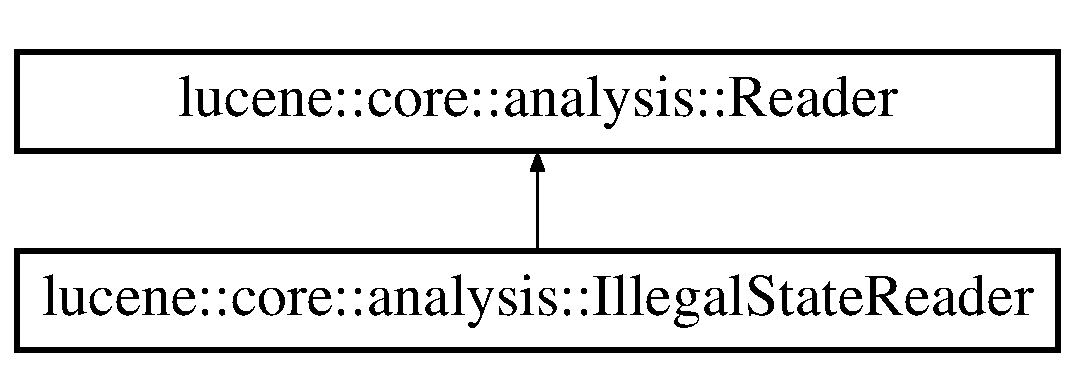
\includegraphics[height=2.000000cm]{classlucene_1_1core_1_1analysis_1_1IllegalStateReader}
\end{center}
\end{figure}
\subsection*{Public Member Functions}
\begin{DoxyCompactItemize}
\item 
virtual \mbox{\hyperlink{classlucene_1_1core_1_1analysis_1_1IllegalStateReader_a9965d5df8761b75e9e5a1dadb5973dbd}{$\sim$\+Illegal\+State\+Reader}} ()
\item 
int \mbox{\hyperlink{classlucene_1_1core_1_1analysis_1_1IllegalStateReader_a9bca98f676ac3d0eeadfd4a2cc78d764}{Read}} ()
\item 
void \mbox{\hyperlink{classlucene_1_1core_1_1analysis_1_1IllegalStateReader_a39217e818ee6678830260a10885400f8}{Read\+Line}} (std\+::string \&line)
\item 
int32\+\_\+t \mbox{\hyperlink{classlucene_1_1core_1_1analysis_1_1IllegalStateReader_a8017ca4fc795b71e16bb87d4a24bdfa9}{Read}} (char $\ast$cstr, \mbox{\hyperlink{ZlibCrc32_8h_a2c212835823e3c54a8ab6d95c652660e}{const}} uint32\+\_\+t off, \mbox{\hyperlink{ZlibCrc32_8h_a2c212835823e3c54a8ab6d95c652660e}{const}} uint32\+\_\+t len)
\item 
void \mbox{\hyperlink{classlucene_1_1core_1_1analysis_1_1IllegalStateReader_aa2a34d98ca51e81297960b13aa0fa18e}{Skip}} (\mbox{\hyperlink{ZlibCrc32_8h_a2c212835823e3c54a8ab6d95c652660e}{const}} uint64\+\_\+t n)
\item 
bool \mbox{\hyperlink{classlucene_1_1core_1_1analysis_1_1IllegalStateReader_ae2de5e9375664ca55c80b224ac3cd998}{Mark\+Supported}} ()
\item 
void \mbox{\hyperlink{classlucene_1_1core_1_1analysis_1_1IllegalStateReader_a96a8cb65743ac1a4db9633b2e0d203fb}{Mark}} (uint32\+\_\+t read\+\_\+ahead\+\_\+limit)
\item 
void \mbox{\hyperlink{classlucene_1_1core_1_1analysis_1_1IllegalStateReader_a7c457898d46f0dcf7de18a1730330c02}{Reset}} ()
\item 
void \mbox{\hyperlink{classlucene_1_1core_1_1analysis_1_1IllegalStateReader_aa92b3c9c3da611e2e44c3edf4078dbe6}{Close}} ()
\item 
bool \mbox{\hyperlink{classlucene_1_1core_1_1analysis_1_1IllegalStateReader_a0f3665a702d4b01dc3298e547379339a}{Eof}} ()
\end{DoxyCompactItemize}


\subsection{Constructor \& Destructor Documentation}
\mbox{\Hypertarget{classlucene_1_1core_1_1analysis_1_1IllegalStateReader_a9965d5df8761b75e9e5a1dadb5973dbd}\label{classlucene_1_1core_1_1analysis_1_1IllegalStateReader_a9965d5df8761b75e9e5a1dadb5973dbd}} 
\index{lucene\+::core\+::analysis\+::\+Illegal\+State\+Reader@{lucene\+::core\+::analysis\+::\+Illegal\+State\+Reader}!````~Illegal\+State\+Reader@{$\sim$\+Illegal\+State\+Reader}}
\index{````~Illegal\+State\+Reader@{$\sim$\+Illegal\+State\+Reader}!lucene\+::core\+::analysis\+::\+Illegal\+State\+Reader@{lucene\+::core\+::analysis\+::\+Illegal\+State\+Reader}}
\subsubsection{\texorpdfstring{$\sim$\+Illegal\+State\+Reader()}{~IllegalStateReader()}}
{\footnotesize\ttfamily virtual lucene\+::core\+::analysis\+::\+Illegal\+State\+Reader\+::$\sim$\+Illegal\+State\+Reader (\begin{DoxyParamCaption}{ }\end{DoxyParamCaption})\hspace{0.3cm}{\ttfamily [inline]}, {\ttfamily [virtual]}}



\subsection{Member Function Documentation}
\mbox{\Hypertarget{classlucene_1_1core_1_1analysis_1_1IllegalStateReader_aa92b3c9c3da611e2e44c3edf4078dbe6}\label{classlucene_1_1core_1_1analysis_1_1IllegalStateReader_aa92b3c9c3da611e2e44c3edf4078dbe6}} 
\index{lucene\+::core\+::analysis\+::\+Illegal\+State\+Reader@{lucene\+::core\+::analysis\+::\+Illegal\+State\+Reader}!Close@{Close}}
\index{Close@{Close}!lucene\+::core\+::analysis\+::\+Illegal\+State\+Reader@{lucene\+::core\+::analysis\+::\+Illegal\+State\+Reader}}
\subsubsection{\texorpdfstring{Close()}{Close()}}
{\footnotesize\ttfamily void lucene\+::core\+::analysis\+::\+Illegal\+State\+Reader\+::\+Close (\begin{DoxyParamCaption}{ }\end{DoxyParamCaption})\hspace{0.3cm}{\ttfamily [inline]}, {\ttfamily [virtual]}}



Implements \mbox{\hyperlink{classlucene_1_1core_1_1analysis_1_1Reader_a4be7e96dccdd3e276e3450e3ad7a70f4}{lucene\+::core\+::analysis\+::\+Reader}}.

\mbox{\Hypertarget{classlucene_1_1core_1_1analysis_1_1IllegalStateReader_a0f3665a702d4b01dc3298e547379339a}\label{classlucene_1_1core_1_1analysis_1_1IllegalStateReader_a0f3665a702d4b01dc3298e547379339a}} 
\index{lucene\+::core\+::analysis\+::\+Illegal\+State\+Reader@{lucene\+::core\+::analysis\+::\+Illegal\+State\+Reader}!Eof@{Eof}}
\index{Eof@{Eof}!lucene\+::core\+::analysis\+::\+Illegal\+State\+Reader@{lucene\+::core\+::analysis\+::\+Illegal\+State\+Reader}}
\subsubsection{\texorpdfstring{Eof()}{Eof()}}
{\footnotesize\ttfamily bool lucene\+::core\+::analysis\+::\+Illegal\+State\+Reader\+::\+Eof (\begin{DoxyParamCaption}{ }\end{DoxyParamCaption})\hspace{0.3cm}{\ttfamily [inline]}, {\ttfamily [virtual]}}



Implements \mbox{\hyperlink{classlucene_1_1core_1_1analysis_1_1Reader_af7a24f3904f9c40e9c5c204b3434f1f7}{lucene\+::core\+::analysis\+::\+Reader}}.

\mbox{\Hypertarget{classlucene_1_1core_1_1analysis_1_1IllegalStateReader_a96a8cb65743ac1a4db9633b2e0d203fb}\label{classlucene_1_1core_1_1analysis_1_1IllegalStateReader_a96a8cb65743ac1a4db9633b2e0d203fb}} 
\index{lucene\+::core\+::analysis\+::\+Illegal\+State\+Reader@{lucene\+::core\+::analysis\+::\+Illegal\+State\+Reader}!Mark@{Mark}}
\index{Mark@{Mark}!lucene\+::core\+::analysis\+::\+Illegal\+State\+Reader@{lucene\+::core\+::analysis\+::\+Illegal\+State\+Reader}}
\subsubsection{\texorpdfstring{Mark()}{Mark()}}
{\footnotesize\ttfamily void lucene\+::core\+::analysis\+::\+Illegal\+State\+Reader\+::\+Mark (\begin{DoxyParamCaption}\item[{uint32\+\_\+t}]{read\+\_\+ahead\+\_\+limit }\end{DoxyParamCaption})\hspace{0.3cm}{\ttfamily [inline]}, {\ttfamily [virtual]}}



Implements \mbox{\hyperlink{classlucene_1_1core_1_1analysis_1_1Reader_a0b60b07a3f65098a50f10f6618097527}{lucene\+::core\+::analysis\+::\+Reader}}.

\mbox{\Hypertarget{classlucene_1_1core_1_1analysis_1_1IllegalStateReader_ae2de5e9375664ca55c80b224ac3cd998}\label{classlucene_1_1core_1_1analysis_1_1IllegalStateReader_ae2de5e9375664ca55c80b224ac3cd998}} 
\index{lucene\+::core\+::analysis\+::\+Illegal\+State\+Reader@{lucene\+::core\+::analysis\+::\+Illegal\+State\+Reader}!Mark\+Supported@{Mark\+Supported}}
\index{Mark\+Supported@{Mark\+Supported}!lucene\+::core\+::analysis\+::\+Illegal\+State\+Reader@{lucene\+::core\+::analysis\+::\+Illegal\+State\+Reader}}
\subsubsection{\texorpdfstring{Mark\+Supported()}{MarkSupported()}}
{\footnotesize\ttfamily bool lucene\+::core\+::analysis\+::\+Illegal\+State\+Reader\+::\+Mark\+Supported (\begin{DoxyParamCaption}{ }\end{DoxyParamCaption})\hspace{0.3cm}{\ttfamily [inline]}, {\ttfamily [virtual]}}



Implements \mbox{\hyperlink{classlucene_1_1core_1_1analysis_1_1Reader_a230fae02ca4a63de33fdaad6f9aafd96}{lucene\+::core\+::analysis\+::\+Reader}}.

\mbox{\Hypertarget{classlucene_1_1core_1_1analysis_1_1IllegalStateReader_a9bca98f676ac3d0eeadfd4a2cc78d764}\label{classlucene_1_1core_1_1analysis_1_1IllegalStateReader_a9bca98f676ac3d0eeadfd4a2cc78d764}} 
\index{lucene\+::core\+::analysis\+::\+Illegal\+State\+Reader@{lucene\+::core\+::analysis\+::\+Illegal\+State\+Reader}!Read@{Read}}
\index{Read@{Read}!lucene\+::core\+::analysis\+::\+Illegal\+State\+Reader@{lucene\+::core\+::analysis\+::\+Illegal\+State\+Reader}}
\subsubsection{\texorpdfstring{Read()}{Read()}\hspace{0.1cm}{\footnotesize\ttfamily [1/2]}}
{\footnotesize\ttfamily int lucene\+::core\+::analysis\+::\+Illegal\+State\+Reader\+::\+Read (\begin{DoxyParamCaption}{ }\end{DoxyParamCaption})\hspace{0.3cm}{\ttfamily [inline]}, {\ttfamily [virtual]}}



Implements \mbox{\hyperlink{classlucene_1_1core_1_1analysis_1_1Reader_ae8e04911b6a4c06bb026ca6e74071cb2}{lucene\+::core\+::analysis\+::\+Reader}}.

\mbox{\Hypertarget{classlucene_1_1core_1_1analysis_1_1IllegalStateReader_a8017ca4fc795b71e16bb87d4a24bdfa9}\label{classlucene_1_1core_1_1analysis_1_1IllegalStateReader_a8017ca4fc795b71e16bb87d4a24bdfa9}} 
\index{lucene\+::core\+::analysis\+::\+Illegal\+State\+Reader@{lucene\+::core\+::analysis\+::\+Illegal\+State\+Reader}!Read@{Read}}
\index{Read@{Read}!lucene\+::core\+::analysis\+::\+Illegal\+State\+Reader@{lucene\+::core\+::analysis\+::\+Illegal\+State\+Reader}}
\subsubsection{\texorpdfstring{Read()}{Read()}\hspace{0.1cm}{\footnotesize\ttfamily [2/2]}}
{\footnotesize\ttfamily int32\+\_\+t lucene\+::core\+::analysis\+::\+Illegal\+State\+Reader\+::\+Read (\begin{DoxyParamCaption}\item[{char $\ast$}]{cstr,  }\item[{\mbox{\hyperlink{ZlibCrc32_8h_a2c212835823e3c54a8ab6d95c652660e}{const}} uint32\+\_\+t}]{off,  }\item[{\mbox{\hyperlink{ZlibCrc32_8h_a2c212835823e3c54a8ab6d95c652660e}{const}} uint32\+\_\+t}]{len }\end{DoxyParamCaption})\hspace{0.3cm}{\ttfamily [inline]}, {\ttfamily [virtual]}}



Implements \mbox{\hyperlink{classlucene_1_1core_1_1analysis_1_1Reader_a986e25a49a947dc113a22c6de033ebe9}{lucene\+::core\+::analysis\+::\+Reader}}.

\mbox{\Hypertarget{classlucene_1_1core_1_1analysis_1_1IllegalStateReader_a39217e818ee6678830260a10885400f8}\label{classlucene_1_1core_1_1analysis_1_1IllegalStateReader_a39217e818ee6678830260a10885400f8}} 
\index{lucene\+::core\+::analysis\+::\+Illegal\+State\+Reader@{lucene\+::core\+::analysis\+::\+Illegal\+State\+Reader}!Read\+Line@{Read\+Line}}
\index{Read\+Line@{Read\+Line}!lucene\+::core\+::analysis\+::\+Illegal\+State\+Reader@{lucene\+::core\+::analysis\+::\+Illegal\+State\+Reader}}
\subsubsection{\texorpdfstring{Read\+Line()}{ReadLine()}}
{\footnotesize\ttfamily void lucene\+::core\+::analysis\+::\+Illegal\+State\+Reader\+::\+Read\+Line (\begin{DoxyParamCaption}\item[{std\+::string \&}]{line }\end{DoxyParamCaption})\hspace{0.3cm}{\ttfamily [inline]}, {\ttfamily [virtual]}}



Implements \mbox{\hyperlink{classlucene_1_1core_1_1analysis_1_1Reader_a475ba046fd74e43a1cce4c4702c791c2}{lucene\+::core\+::analysis\+::\+Reader}}.

\mbox{\Hypertarget{classlucene_1_1core_1_1analysis_1_1IllegalStateReader_a7c457898d46f0dcf7de18a1730330c02}\label{classlucene_1_1core_1_1analysis_1_1IllegalStateReader_a7c457898d46f0dcf7de18a1730330c02}} 
\index{lucene\+::core\+::analysis\+::\+Illegal\+State\+Reader@{lucene\+::core\+::analysis\+::\+Illegal\+State\+Reader}!Reset@{Reset}}
\index{Reset@{Reset}!lucene\+::core\+::analysis\+::\+Illegal\+State\+Reader@{lucene\+::core\+::analysis\+::\+Illegal\+State\+Reader}}
\subsubsection{\texorpdfstring{Reset()}{Reset()}}
{\footnotesize\ttfamily void lucene\+::core\+::analysis\+::\+Illegal\+State\+Reader\+::\+Reset (\begin{DoxyParamCaption}{ }\end{DoxyParamCaption})\hspace{0.3cm}{\ttfamily [inline]}, {\ttfamily [virtual]}}



Implements \mbox{\hyperlink{classlucene_1_1core_1_1analysis_1_1Reader_a5299f5469ce4ea9812ec79a59667945a}{lucene\+::core\+::analysis\+::\+Reader}}.

\mbox{\Hypertarget{classlucene_1_1core_1_1analysis_1_1IllegalStateReader_aa2a34d98ca51e81297960b13aa0fa18e}\label{classlucene_1_1core_1_1analysis_1_1IllegalStateReader_aa2a34d98ca51e81297960b13aa0fa18e}} 
\index{lucene\+::core\+::analysis\+::\+Illegal\+State\+Reader@{lucene\+::core\+::analysis\+::\+Illegal\+State\+Reader}!Skip@{Skip}}
\index{Skip@{Skip}!lucene\+::core\+::analysis\+::\+Illegal\+State\+Reader@{lucene\+::core\+::analysis\+::\+Illegal\+State\+Reader}}
\subsubsection{\texorpdfstring{Skip()}{Skip()}}
{\footnotesize\ttfamily void lucene\+::core\+::analysis\+::\+Illegal\+State\+Reader\+::\+Skip (\begin{DoxyParamCaption}\item[{\mbox{\hyperlink{ZlibCrc32_8h_a2c212835823e3c54a8ab6d95c652660e}{const}} uint64\+\_\+t}]{n }\end{DoxyParamCaption})\hspace{0.3cm}{\ttfamily [inline]}, {\ttfamily [virtual]}}



Implements \mbox{\hyperlink{classlucene_1_1core_1_1analysis_1_1Reader_a3bd8e9f3e1d07d698bccabde41970219}{lucene\+::core\+::analysis\+::\+Reader}}.



The documentation for this class was generated from the following file\+:\begin{DoxyCompactItemize}
\item 
Analysis/\mbox{\hyperlink{Reader_8h}{Reader.\+h}}\end{DoxyCompactItemize}

\hypertarget{classlucene_1_1core_1_1analysis_1_1tokenattributes_1_1KeywordAttribute}{}\section{lucene\+:\+:core\+:\+:analysis\+:\+:tokenattributes\+:\+:Keyword\+Attribute Class Reference}
\label{classlucene_1_1core_1_1analysis_1_1tokenattributes_1_1KeywordAttribute}\index{lucene\+::core\+::analysis\+::tokenattributes\+::\+Keyword\+Attribute@{lucene\+::core\+::analysis\+::tokenattributes\+::\+Keyword\+Attribute}}


{\ttfamily \#include $<$Attribute.\+h$>$}

Inheritance diagram for lucene\+:\+:core\+:\+:analysis\+:\+:tokenattributes\+:\+:Keyword\+Attribute\+:\begin{figure}[H]
\begin{center}
\leavevmode
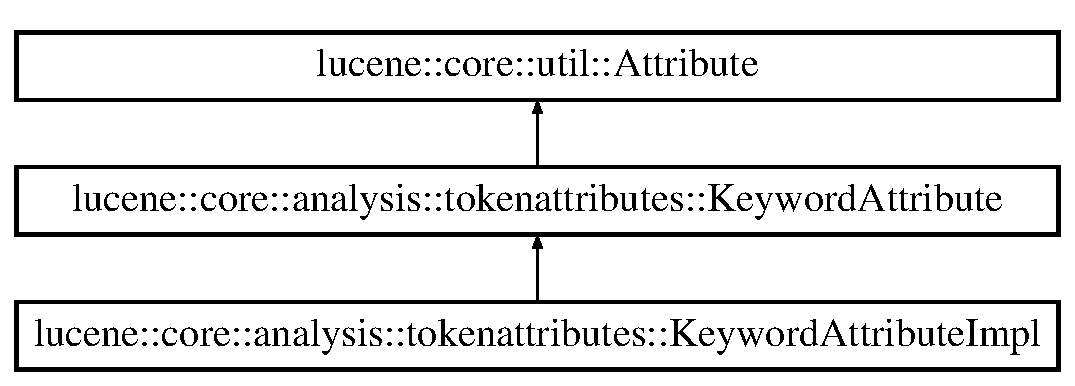
\includegraphics[height=3.000000cm]{classlucene_1_1core_1_1analysis_1_1tokenattributes_1_1KeywordAttribute}
\end{center}
\end{figure}
\subsection*{Public Member Functions}
\begin{DoxyCompactItemize}
\item 
virtual \mbox{\hyperlink{classlucene_1_1core_1_1analysis_1_1tokenattributes_1_1KeywordAttribute_ad4ee53eaa0a2bd3b32e3f94c7be179e7}{$\sim$\+Keyword\+Attribute}} ()
\item 
virtual bool \mbox{\hyperlink{classlucene_1_1core_1_1analysis_1_1tokenattributes_1_1KeywordAttribute_af6270bf727324f1809a18a1fc9b1a27c}{Is\+Keyword}} ()=0
\item 
virtual void \mbox{\hyperlink{classlucene_1_1core_1_1analysis_1_1tokenattributes_1_1KeywordAttribute_aee23c674ba6af03521985734f739c9d5}{Set\+Keyword}} (const bool is\+\_\+keyword)=0
\end{DoxyCompactItemize}
\subsection*{Additional Inherited Members}


\subsection{Constructor \& Destructor Documentation}
\mbox{\Hypertarget{classlucene_1_1core_1_1analysis_1_1tokenattributes_1_1KeywordAttribute_ad4ee53eaa0a2bd3b32e3f94c7be179e7}\label{classlucene_1_1core_1_1analysis_1_1tokenattributes_1_1KeywordAttribute_ad4ee53eaa0a2bd3b32e3f94c7be179e7}} 
\index{lucene\+::core\+::analysis\+::tokenattributes\+::\+Keyword\+Attribute@{lucene\+::core\+::analysis\+::tokenattributes\+::\+Keyword\+Attribute}!````~Keyword\+Attribute@{$\sim$\+Keyword\+Attribute}}
\index{````~Keyword\+Attribute@{$\sim$\+Keyword\+Attribute}!lucene\+::core\+::analysis\+::tokenattributes\+::\+Keyword\+Attribute@{lucene\+::core\+::analysis\+::tokenattributes\+::\+Keyword\+Attribute}}
\subsubsection{\texorpdfstring{$\sim$\+Keyword\+Attribute()}{~KeywordAttribute()}}
{\footnotesize\ttfamily virtual lucene\+::core\+::analysis\+::tokenattributes\+::\+Keyword\+Attribute\+::$\sim$\+Keyword\+Attribute (\begin{DoxyParamCaption}{ }\end{DoxyParamCaption})\hspace{0.3cm}{\ttfamily [inline]}, {\ttfamily [virtual]}}



\subsection{Member Function Documentation}
\mbox{\Hypertarget{classlucene_1_1core_1_1analysis_1_1tokenattributes_1_1KeywordAttribute_af6270bf727324f1809a18a1fc9b1a27c}\label{classlucene_1_1core_1_1analysis_1_1tokenattributes_1_1KeywordAttribute_af6270bf727324f1809a18a1fc9b1a27c}} 
\index{lucene\+::core\+::analysis\+::tokenattributes\+::\+Keyword\+Attribute@{lucene\+::core\+::analysis\+::tokenattributes\+::\+Keyword\+Attribute}!Is\+Keyword@{Is\+Keyword}}
\index{Is\+Keyword@{Is\+Keyword}!lucene\+::core\+::analysis\+::tokenattributes\+::\+Keyword\+Attribute@{lucene\+::core\+::analysis\+::tokenattributes\+::\+Keyword\+Attribute}}
\subsubsection{\texorpdfstring{Is\+Keyword()}{IsKeyword()}}
{\footnotesize\ttfamily virtual bool lucene\+::core\+::analysis\+::tokenattributes\+::\+Keyword\+Attribute\+::\+Is\+Keyword (\begin{DoxyParamCaption}{ }\end{DoxyParamCaption})\hspace{0.3cm}{\ttfamily [pure virtual]}}



Implemented in \mbox{\hyperlink{classlucene_1_1core_1_1analysis_1_1tokenattributes_1_1KeywordAttributeImpl_aa98aa28fbea635057a71d0129cb92a2e}{lucene\+::core\+::analysis\+::tokenattributes\+::\+Keyword\+Attribute\+Impl}}.

\mbox{\Hypertarget{classlucene_1_1core_1_1analysis_1_1tokenattributes_1_1KeywordAttribute_aee23c674ba6af03521985734f739c9d5}\label{classlucene_1_1core_1_1analysis_1_1tokenattributes_1_1KeywordAttribute_aee23c674ba6af03521985734f739c9d5}} 
\index{lucene\+::core\+::analysis\+::tokenattributes\+::\+Keyword\+Attribute@{lucene\+::core\+::analysis\+::tokenattributes\+::\+Keyword\+Attribute}!Set\+Keyword@{Set\+Keyword}}
\index{Set\+Keyword@{Set\+Keyword}!lucene\+::core\+::analysis\+::tokenattributes\+::\+Keyword\+Attribute@{lucene\+::core\+::analysis\+::tokenattributes\+::\+Keyword\+Attribute}}
\subsubsection{\texorpdfstring{Set\+Keyword()}{SetKeyword()}}
{\footnotesize\ttfamily virtual void lucene\+::core\+::analysis\+::tokenattributes\+::\+Keyword\+Attribute\+::\+Set\+Keyword (\begin{DoxyParamCaption}\item[{const bool}]{is\+\_\+keyword }\end{DoxyParamCaption})\hspace{0.3cm}{\ttfamily [pure virtual]}}



Implemented in \mbox{\hyperlink{classlucene_1_1core_1_1analysis_1_1tokenattributes_1_1KeywordAttributeImpl_a1cae85f0e103d3dfa054c1a42e119de2}{lucene\+::core\+::analysis\+::tokenattributes\+::\+Keyword\+Attribute\+Impl}}.



The documentation for this class was generated from the following file\+:\begin{DoxyCompactItemize}
\item 
Analysis/\mbox{\hyperlink{Analysis_2Attribute_8h}{Attribute.\+h}}\end{DoxyCompactItemize}

\hypertarget{classlucene_1_1core_1_1analysis_1_1tokenattributes_1_1KeywordAttributeImpl}{}\section{lucene\+:\+:core\+:\+:analysis\+:\+:tokenattributes\+:\+:Keyword\+Attribute\+Impl Class Reference}
\label{classlucene_1_1core_1_1analysis_1_1tokenattributes_1_1KeywordAttributeImpl}\index{lucene\+::core\+::analysis\+::tokenattributes\+::\+Keyword\+Attribute\+Impl@{lucene\+::core\+::analysis\+::tokenattributes\+::\+Keyword\+Attribute\+Impl}}


{\ttfamily \#include $<$Attribute\+Impl.\+h$>$}

Inheritance diagram for lucene\+:\+:core\+:\+:analysis\+:\+:tokenattributes\+:\+:Keyword\+Attribute\+Impl\+:\begin{figure}[H]
\begin{center}
\leavevmode
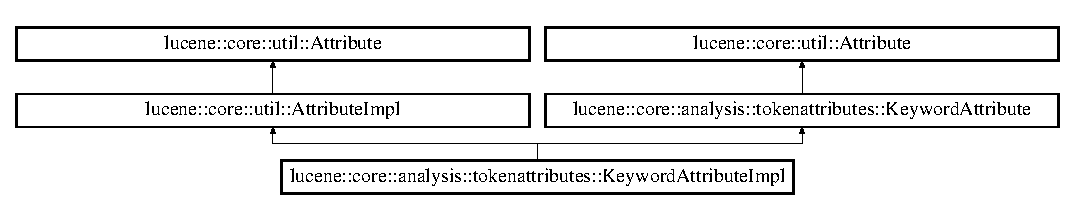
\includegraphics[height=2.372881cm]{classlucene_1_1core_1_1analysis_1_1tokenattributes_1_1KeywordAttributeImpl}
\end{center}
\end{figure}
\subsection*{Public Member Functions}
\begin{DoxyCompactItemize}
\item 
\mbox{\hyperlink{classlucene_1_1core_1_1analysis_1_1tokenattributes_1_1KeywordAttributeImpl_a1a92ef5f629fcca79c12a5009deb7941}{Keyword\+Attribute\+Impl}} ()
\item 
\mbox{\hyperlink{classlucene_1_1core_1_1analysis_1_1tokenattributes_1_1KeywordAttributeImpl_a8737063d5e2cb8ad21fdba8ec4ba210f}{Keyword\+Attribute\+Impl}} (const \mbox{\hyperlink{classlucene_1_1core_1_1analysis_1_1tokenattributes_1_1KeywordAttributeImpl}{Keyword\+Attribute\+Impl}} \&other)
\item 
virtual \mbox{\hyperlink{classlucene_1_1core_1_1analysis_1_1tokenattributes_1_1KeywordAttributeImpl_aab9c236453177ca4e9c3cb86d3e93fa6}{$\sim$\+Keyword\+Attribute\+Impl}} ()
\item 
bool \mbox{\hyperlink{classlucene_1_1core_1_1analysis_1_1tokenattributes_1_1KeywordAttributeImpl_aa98aa28fbea635057a71d0129cb92a2e}{Is\+Keyword}} () override
\item 
void \mbox{\hyperlink{classlucene_1_1core_1_1analysis_1_1tokenattributes_1_1KeywordAttributeImpl_a1cae85f0e103d3dfa054c1a42e119de2}{Set\+Keyword}} (const bool is\+\_\+keyword) override
\item 
void \mbox{\hyperlink{classlucene_1_1core_1_1analysis_1_1tokenattributes_1_1KeywordAttributeImpl_a610aab1880b02caf13fb7f1723c24c94}{Reflect\+With}} (\mbox{\hyperlink{namespacelucene_1_1core_1_1util_a7dbb701adaed055f73fb95eec83da10a}{lucene\+::core\+::util\+::\+Attribute\+Reflector}} \&reflector) override
\item 
void \mbox{\hyperlink{classlucene_1_1core_1_1analysis_1_1tokenattributes_1_1KeywordAttributeImpl_a019bfed2dce94170444db84c7575f43c}{Clear}} () override
\item 
bool \mbox{\hyperlink{classlucene_1_1core_1_1analysis_1_1tokenattributes_1_1KeywordAttributeImpl_a057cd81b19aa11973911473903ff84e3}{operator==}} (const \mbox{\hyperlink{classlucene_1_1core_1_1analysis_1_1tokenattributes_1_1KeywordAttributeImpl}{Keyword\+Attribute\+Impl}} \&other) const
\item 
std\+::vector$<$ std\+::type\+\_\+index $>$ \mbox{\hyperlink{classlucene_1_1core_1_1analysis_1_1tokenattributes_1_1KeywordAttributeImpl_af338dde5485b5feb1b467fc07534f5cc}{Attributes}} () override
\item 
void \mbox{\hyperlink{classlucene_1_1core_1_1analysis_1_1tokenattributes_1_1KeywordAttributeImpl_a83f442881b35bc26a6edb2e04beeb58a}{Shallow\+Copy\+To}} (\mbox{\hyperlink{classlucene_1_1core_1_1util_1_1AttributeImpl}{lucene\+::core\+::util\+::\+Attribute\+Impl}} \&attr\+\_\+impl) override
\item 
\mbox{\hyperlink{classlucene_1_1core_1_1analysis_1_1tokenattributes_1_1KeywordAttributeImpl}{Keyword\+Attribute\+Impl}} \& \mbox{\hyperlink{classlucene_1_1core_1_1analysis_1_1tokenattributes_1_1KeywordAttributeImpl_a30228ce41cc678c1cb85c2fb1179f447}{operator=}} (const \mbox{\hyperlink{classlucene_1_1core_1_1util_1_1AttributeImpl}{lucene\+::core\+::util\+::\+Attribute\+Impl}} \&other)
\item 
\mbox{\hyperlink{classlucene_1_1core_1_1analysis_1_1tokenattributes_1_1KeywordAttributeImpl}{Keyword\+Attribute\+Impl}} \& \mbox{\hyperlink{classlucene_1_1core_1_1analysis_1_1tokenattributes_1_1KeywordAttributeImpl_a26caf7be7512728452c2a5496788c39c}{operator=}} (const \mbox{\hyperlink{classlucene_1_1core_1_1analysis_1_1tokenattributes_1_1KeywordAttributeImpl}{Keyword\+Attribute\+Impl}} \&other)
\item 
\mbox{\hyperlink{classlucene_1_1core_1_1util_1_1AttributeImpl}{Attribute\+Impl}} $\ast$ \mbox{\hyperlink{classlucene_1_1core_1_1analysis_1_1tokenattributes_1_1KeywordAttributeImpl_a59d16bdfa3c456ebcd8b3ae90279cd7b}{Clone}} () override
\end{DoxyCompactItemize}
\subsection*{Private Attributes}
\begin{DoxyCompactItemize}
\item 
bool \mbox{\hyperlink{classlucene_1_1core_1_1analysis_1_1tokenattributes_1_1KeywordAttributeImpl_a126e0c7f8c8c863cc2600f89ebade88d}{keyword}}
\end{DoxyCompactItemize}
\subsection*{Additional Inherited Members}


\subsection{Constructor \& Destructor Documentation}
\mbox{\Hypertarget{classlucene_1_1core_1_1analysis_1_1tokenattributes_1_1KeywordAttributeImpl_a1a92ef5f629fcca79c12a5009deb7941}\label{classlucene_1_1core_1_1analysis_1_1tokenattributes_1_1KeywordAttributeImpl_a1a92ef5f629fcca79c12a5009deb7941}} 
\index{lucene\+::core\+::analysis\+::tokenattributes\+::\+Keyword\+Attribute\+Impl@{lucene\+::core\+::analysis\+::tokenattributes\+::\+Keyword\+Attribute\+Impl}!Keyword\+Attribute\+Impl@{Keyword\+Attribute\+Impl}}
\index{Keyword\+Attribute\+Impl@{Keyword\+Attribute\+Impl}!lucene\+::core\+::analysis\+::tokenattributes\+::\+Keyword\+Attribute\+Impl@{lucene\+::core\+::analysis\+::tokenattributes\+::\+Keyword\+Attribute\+Impl}}
\subsubsection{\texorpdfstring{Keyword\+Attribute\+Impl()}{KeywordAttributeImpl()}\hspace{0.1cm}{\footnotesize\ttfamily [1/2]}}
{\footnotesize\ttfamily Keyword\+Attribute\+Impl\+::\+Keyword\+Attribute\+Impl (\begin{DoxyParamCaption}{ }\end{DoxyParamCaption})}

\mbox{\hyperlink{classlucene_1_1core_1_1analysis_1_1tokenattributes_1_1KeywordAttributeImpl}{Keyword\+Attribute\+Impl}} \mbox{\Hypertarget{classlucene_1_1core_1_1analysis_1_1tokenattributes_1_1KeywordAttributeImpl_a8737063d5e2cb8ad21fdba8ec4ba210f}\label{classlucene_1_1core_1_1analysis_1_1tokenattributes_1_1KeywordAttributeImpl_a8737063d5e2cb8ad21fdba8ec4ba210f}} 
\index{lucene\+::core\+::analysis\+::tokenattributes\+::\+Keyword\+Attribute\+Impl@{lucene\+::core\+::analysis\+::tokenattributes\+::\+Keyword\+Attribute\+Impl}!Keyword\+Attribute\+Impl@{Keyword\+Attribute\+Impl}}
\index{Keyword\+Attribute\+Impl@{Keyword\+Attribute\+Impl}!lucene\+::core\+::analysis\+::tokenattributes\+::\+Keyword\+Attribute\+Impl@{lucene\+::core\+::analysis\+::tokenattributes\+::\+Keyword\+Attribute\+Impl}}
\subsubsection{\texorpdfstring{Keyword\+Attribute\+Impl()}{KeywordAttributeImpl()}\hspace{0.1cm}{\footnotesize\ttfamily [2/2]}}
{\footnotesize\ttfamily Keyword\+Attribute\+Impl\+::\+Keyword\+Attribute\+Impl (\begin{DoxyParamCaption}\item[{const \mbox{\hyperlink{classlucene_1_1core_1_1analysis_1_1tokenattributes_1_1KeywordAttributeImpl}{Keyword\+Attribute\+Impl}} \&}]{other }\end{DoxyParamCaption})}

\mbox{\Hypertarget{classlucene_1_1core_1_1analysis_1_1tokenattributes_1_1KeywordAttributeImpl_aab9c236453177ca4e9c3cb86d3e93fa6}\label{classlucene_1_1core_1_1analysis_1_1tokenattributes_1_1KeywordAttributeImpl_aab9c236453177ca4e9c3cb86d3e93fa6}} 
\index{lucene\+::core\+::analysis\+::tokenattributes\+::\+Keyword\+Attribute\+Impl@{lucene\+::core\+::analysis\+::tokenattributes\+::\+Keyword\+Attribute\+Impl}!````~Keyword\+Attribute\+Impl@{$\sim$\+Keyword\+Attribute\+Impl}}
\index{````~Keyword\+Attribute\+Impl@{$\sim$\+Keyword\+Attribute\+Impl}!lucene\+::core\+::analysis\+::tokenattributes\+::\+Keyword\+Attribute\+Impl@{lucene\+::core\+::analysis\+::tokenattributes\+::\+Keyword\+Attribute\+Impl}}
\subsubsection{\texorpdfstring{$\sim$\+Keyword\+Attribute\+Impl()}{~KeywordAttributeImpl()}}
{\footnotesize\ttfamily Keyword\+Attribute\+Impl\+::$\sim$\+Keyword\+Attribute\+Impl (\begin{DoxyParamCaption}{ }\end{DoxyParamCaption})\hspace{0.3cm}{\ttfamily [virtual]}}



\subsection{Member Function Documentation}
\mbox{\Hypertarget{classlucene_1_1core_1_1analysis_1_1tokenattributes_1_1KeywordAttributeImpl_af338dde5485b5feb1b467fc07534f5cc}\label{classlucene_1_1core_1_1analysis_1_1tokenattributes_1_1KeywordAttributeImpl_af338dde5485b5feb1b467fc07534f5cc}} 
\index{lucene\+::core\+::analysis\+::tokenattributes\+::\+Keyword\+Attribute\+Impl@{lucene\+::core\+::analysis\+::tokenattributes\+::\+Keyword\+Attribute\+Impl}!Attributes@{Attributes}}
\index{Attributes@{Attributes}!lucene\+::core\+::analysis\+::tokenattributes\+::\+Keyword\+Attribute\+Impl@{lucene\+::core\+::analysis\+::tokenattributes\+::\+Keyword\+Attribute\+Impl}}
\subsubsection{\texorpdfstring{Attributes()}{Attributes()}}
{\footnotesize\ttfamily std\+::vector$<$ std\+::type\+\_\+index $>$ Keyword\+Attribute\+Impl\+::\+Attributes (\begin{DoxyParamCaption}{ }\end{DoxyParamCaption})\hspace{0.3cm}{\ttfamily [override]}, {\ttfamily [virtual]}}



Implements \mbox{\hyperlink{classlucene_1_1core_1_1util_1_1AttributeImpl_ac0631e6a7a11044883bc97447716d7cc}{lucene\+::core\+::util\+::\+Attribute\+Impl}}.

\mbox{\Hypertarget{classlucene_1_1core_1_1analysis_1_1tokenattributes_1_1KeywordAttributeImpl_a019bfed2dce94170444db84c7575f43c}\label{classlucene_1_1core_1_1analysis_1_1tokenattributes_1_1KeywordAttributeImpl_a019bfed2dce94170444db84c7575f43c}} 
\index{lucene\+::core\+::analysis\+::tokenattributes\+::\+Keyword\+Attribute\+Impl@{lucene\+::core\+::analysis\+::tokenattributes\+::\+Keyword\+Attribute\+Impl}!Clear@{Clear}}
\index{Clear@{Clear}!lucene\+::core\+::analysis\+::tokenattributes\+::\+Keyword\+Attribute\+Impl@{lucene\+::core\+::analysis\+::tokenattributes\+::\+Keyword\+Attribute\+Impl}}
\subsubsection{\texorpdfstring{Clear()}{Clear()}}
{\footnotesize\ttfamily void Keyword\+Attribute\+Impl\+::\+Clear (\begin{DoxyParamCaption}{ }\end{DoxyParamCaption})\hspace{0.3cm}{\ttfamily [override]}, {\ttfamily [virtual]}}



Implements \mbox{\hyperlink{classlucene_1_1core_1_1util_1_1AttributeImpl_a04897a00a902f7a345dd44bbc4b482a8}{lucene\+::core\+::util\+::\+Attribute\+Impl}}.

\mbox{\Hypertarget{classlucene_1_1core_1_1analysis_1_1tokenattributes_1_1KeywordAttributeImpl_a59d16bdfa3c456ebcd8b3ae90279cd7b}\label{classlucene_1_1core_1_1analysis_1_1tokenattributes_1_1KeywordAttributeImpl_a59d16bdfa3c456ebcd8b3ae90279cd7b}} 
\index{lucene\+::core\+::analysis\+::tokenattributes\+::\+Keyword\+Attribute\+Impl@{lucene\+::core\+::analysis\+::tokenattributes\+::\+Keyword\+Attribute\+Impl}!Clone@{Clone}}
\index{Clone@{Clone}!lucene\+::core\+::analysis\+::tokenattributes\+::\+Keyword\+Attribute\+Impl@{lucene\+::core\+::analysis\+::tokenattributes\+::\+Keyword\+Attribute\+Impl}}
\subsubsection{\texorpdfstring{Clone()}{Clone()}}
{\footnotesize\ttfamily \mbox{\hyperlink{classlucene_1_1core_1_1util_1_1AttributeImpl}{Attribute\+Impl}} $\ast$ Keyword\+Attribute\+Impl\+::\+Clone (\begin{DoxyParamCaption}{ }\end{DoxyParamCaption})\hspace{0.3cm}{\ttfamily [override]}, {\ttfamily [virtual]}}



Implements \mbox{\hyperlink{classlucene_1_1core_1_1util_1_1AttributeImpl_a135318ad4c7c17b3d85e625e32fb42cd}{lucene\+::core\+::util\+::\+Attribute\+Impl}}.

\mbox{\Hypertarget{classlucene_1_1core_1_1analysis_1_1tokenattributes_1_1KeywordAttributeImpl_aa98aa28fbea635057a71d0129cb92a2e}\label{classlucene_1_1core_1_1analysis_1_1tokenattributes_1_1KeywordAttributeImpl_aa98aa28fbea635057a71d0129cb92a2e}} 
\index{lucene\+::core\+::analysis\+::tokenattributes\+::\+Keyword\+Attribute\+Impl@{lucene\+::core\+::analysis\+::tokenattributes\+::\+Keyword\+Attribute\+Impl}!Is\+Keyword@{Is\+Keyword}}
\index{Is\+Keyword@{Is\+Keyword}!lucene\+::core\+::analysis\+::tokenattributes\+::\+Keyword\+Attribute\+Impl@{lucene\+::core\+::analysis\+::tokenattributes\+::\+Keyword\+Attribute\+Impl}}
\subsubsection{\texorpdfstring{Is\+Keyword()}{IsKeyword()}}
{\footnotesize\ttfamily bool Keyword\+Attribute\+Impl\+::\+Is\+Keyword (\begin{DoxyParamCaption}{ }\end{DoxyParamCaption})\hspace{0.3cm}{\ttfamily [override]}, {\ttfamily [virtual]}}



Implements \mbox{\hyperlink{classlucene_1_1core_1_1analysis_1_1tokenattributes_1_1KeywordAttribute_af6270bf727324f1809a18a1fc9b1a27c}{lucene\+::core\+::analysis\+::tokenattributes\+::\+Keyword\+Attribute}}.

\mbox{\Hypertarget{classlucene_1_1core_1_1analysis_1_1tokenattributes_1_1KeywordAttributeImpl_a30228ce41cc678c1cb85c2fb1179f447}\label{classlucene_1_1core_1_1analysis_1_1tokenattributes_1_1KeywordAttributeImpl_a30228ce41cc678c1cb85c2fb1179f447}} 
\index{lucene\+::core\+::analysis\+::tokenattributes\+::\+Keyword\+Attribute\+Impl@{lucene\+::core\+::analysis\+::tokenattributes\+::\+Keyword\+Attribute\+Impl}!operator=@{operator=}}
\index{operator=@{operator=}!lucene\+::core\+::analysis\+::tokenattributes\+::\+Keyword\+Attribute\+Impl@{lucene\+::core\+::analysis\+::tokenattributes\+::\+Keyword\+Attribute\+Impl}}
\subsubsection{\texorpdfstring{operator=()}{operator=()}\hspace{0.1cm}{\footnotesize\ttfamily [1/2]}}
{\footnotesize\ttfamily \mbox{\hyperlink{classlucene_1_1core_1_1analysis_1_1tokenattributes_1_1KeywordAttributeImpl}{Keyword\+Attribute\+Impl}} \& Keyword\+Attribute\+Impl\+::operator= (\begin{DoxyParamCaption}\item[{const \mbox{\hyperlink{classlucene_1_1core_1_1util_1_1AttributeImpl}{lucene\+::core\+::util\+::\+Attribute\+Impl}} \&}]{other }\end{DoxyParamCaption})\hspace{0.3cm}{\ttfamily [virtual]}}



Implements \mbox{\hyperlink{classlucene_1_1core_1_1util_1_1AttributeImpl_ab032e399d03ce2f58c76881cf2b92325}{lucene\+::core\+::util\+::\+Attribute\+Impl}}.

\mbox{\Hypertarget{classlucene_1_1core_1_1analysis_1_1tokenattributes_1_1KeywordAttributeImpl_a26caf7be7512728452c2a5496788c39c}\label{classlucene_1_1core_1_1analysis_1_1tokenattributes_1_1KeywordAttributeImpl_a26caf7be7512728452c2a5496788c39c}} 
\index{lucene\+::core\+::analysis\+::tokenattributes\+::\+Keyword\+Attribute\+Impl@{lucene\+::core\+::analysis\+::tokenattributes\+::\+Keyword\+Attribute\+Impl}!operator=@{operator=}}
\index{operator=@{operator=}!lucene\+::core\+::analysis\+::tokenattributes\+::\+Keyword\+Attribute\+Impl@{lucene\+::core\+::analysis\+::tokenattributes\+::\+Keyword\+Attribute\+Impl}}
\subsubsection{\texorpdfstring{operator=()}{operator=()}\hspace{0.1cm}{\footnotesize\ttfamily [2/2]}}
{\footnotesize\ttfamily \mbox{\hyperlink{classlucene_1_1core_1_1analysis_1_1tokenattributes_1_1KeywordAttributeImpl}{Keyword\+Attribute\+Impl}} \& Keyword\+Attribute\+Impl\+::operator= (\begin{DoxyParamCaption}\item[{const \mbox{\hyperlink{classlucene_1_1core_1_1analysis_1_1tokenattributes_1_1KeywordAttributeImpl}{Keyword\+Attribute\+Impl}} \&}]{other }\end{DoxyParamCaption})}

\mbox{\Hypertarget{classlucene_1_1core_1_1analysis_1_1tokenattributes_1_1KeywordAttributeImpl_a057cd81b19aa11973911473903ff84e3}\label{classlucene_1_1core_1_1analysis_1_1tokenattributes_1_1KeywordAttributeImpl_a057cd81b19aa11973911473903ff84e3}} 
\index{lucene\+::core\+::analysis\+::tokenattributes\+::\+Keyword\+Attribute\+Impl@{lucene\+::core\+::analysis\+::tokenattributes\+::\+Keyword\+Attribute\+Impl}!operator==@{operator==}}
\index{operator==@{operator==}!lucene\+::core\+::analysis\+::tokenattributes\+::\+Keyword\+Attribute\+Impl@{lucene\+::core\+::analysis\+::tokenattributes\+::\+Keyword\+Attribute\+Impl}}
\subsubsection{\texorpdfstring{operator==()}{operator==()}}
{\footnotesize\ttfamily bool Keyword\+Attribute\+Impl\+::operator== (\begin{DoxyParamCaption}\item[{const \mbox{\hyperlink{classlucene_1_1core_1_1analysis_1_1tokenattributes_1_1KeywordAttributeImpl}{Keyword\+Attribute\+Impl}} \&}]{other }\end{DoxyParamCaption}) const}

\mbox{\Hypertarget{classlucene_1_1core_1_1analysis_1_1tokenattributes_1_1KeywordAttributeImpl_a610aab1880b02caf13fb7f1723c24c94}\label{classlucene_1_1core_1_1analysis_1_1tokenattributes_1_1KeywordAttributeImpl_a610aab1880b02caf13fb7f1723c24c94}} 
\index{lucene\+::core\+::analysis\+::tokenattributes\+::\+Keyword\+Attribute\+Impl@{lucene\+::core\+::analysis\+::tokenattributes\+::\+Keyword\+Attribute\+Impl}!Reflect\+With@{Reflect\+With}}
\index{Reflect\+With@{Reflect\+With}!lucene\+::core\+::analysis\+::tokenattributes\+::\+Keyword\+Attribute\+Impl@{lucene\+::core\+::analysis\+::tokenattributes\+::\+Keyword\+Attribute\+Impl}}
\subsubsection{\texorpdfstring{Reflect\+With()}{ReflectWith()}}
{\footnotesize\ttfamily void Keyword\+Attribute\+Impl\+::\+Reflect\+With (\begin{DoxyParamCaption}\item[{\mbox{\hyperlink{namespacelucene_1_1core_1_1util_a7dbb701adaed055f73fb95eec83da10a}{lucene\+::core\+::util\+::\+Attribute\+Reflector}} \&}]{reflector }\end{DoxyParamCaption})\hspace{0.3cm}{\ttfamily [override]}, {\ttfamily [virtual]}}



Implements \mbox{\hyperlink{classlucene_1_1core_1_1util_1_1AttributeImpl_a84d34275fb1ed67ac36fad7ff6388096}{lucene\+::core\+::util\+::\+Attribute\+Impl}}.

\mbox{\Hypertarget{classlucene_1_1core_1_1analysis_1_1tokenattributes_1_1KeywordAttributeImpl_a1cae85f0e103d3dfa054c1a42e119de2}\label{classlucene_1_1core_1_1analysis_1_1tokenattributes_1_1KeywordAttributeImpl_a1cae85f0e103d3dfa054c1a42e119de2}} 
\index{lucene\+::core\+::analysis\+::tokenattributes\+::\+Keyword\+Attribute\+Impl@{lucene\+::core\+::analysis\+::tokenattributes\+::\+Keyword\+Attribute\+Impl}!Set\+Keyword@{Set\+Keyword}}
\index{Set\+Keyword@{Set\+Keyword}!lucene\+::core\+::analysis\+::tokenattributes\+::\+Keyword\+Attribute\+Impl@{lucene\+::core\+::analysis\+::tokenattributes\+::\+Keyword\+Attribute\+Impl}}
\subsubsection{\texorpdfstring{Set\+Keyword()}{SetKeyword()}}
{\footnotesize\ttfamily void Keyword\+Attribute\+Impl\+::\+Set\+Keyword (\begin{DoxyParamCaption}\item[{const bool}]{is\+\_\+keyword }\end{DoxyParamCaption})\hspace{0.3cm}{\ttfamily [override]}, {\ttfamily [virtual]}}



Implements \mbox{\hyperlink{classlucene_1_1core_1_1analysis_1_1tokenattributes_1_1KeywordAttribute_aee23c674ba6af03521985734f739c9d5}{lucene\+::core\+::analysis\+::tokenattributes\+::\+Keyword\+Attribute}}.

\mbox{\Hypertarget{classlucene_1_1core_1_1analysis_1_1tokenattributes_1_1KeywordAttributeImpl_a83f442881b35bc26a6edb2e04beeb58a}\label{classlucene_1_1core_1_1analysis_1_1tokenattributes_1_1KeywordAttributeImpl_a83f442881b35bc26a6edb2e04beeb58a}} 
\index{lucene\+::core\+::analysis\+::tokenattributes\+::\+Keyword\+Attribute\+Impl@{lucene\+::core\+::analysis\+::tokenattributes\+::\+Keyword\+Attribute\+Impl}!Shallow\+Copy\+To@{Shallow\+Copy\+To}}
\index{Shallow\+Copy\+To@{Shallow\+Copy\+To}!lucene\+::core\+::analysis\+::tokenattributes\+::\+Keyword\+Attribute\+Impl@{lucene\+::core\+::analysis\+::tokenattributes\+::\+Keyword\+Attribute\+Impl}}
\subsubsection{\texorpdfstring{Shallow\+Copy\+To()}{ShallowCopyTo()}}
{\footnotesize\ttfamily void Keyword\+Attribute\+Impl\+::\+Shallow\+Copy\+To (\begin{DoxyParamCaption}\item[{\mbox{\hyperlink{classlucene_1_1core_1_1util_1_1AttributeImpl}{lucene\+::core\+::util\+::\+Attribute\+Impl}} \&}]{attr\+\_\+impl }\end{DoxyParamCaption})\hspace{0.3cm}{\ttfamily [override]}, {\ttfamily [virtual]}}



Implements \mbox{\hyperlink{classlucene_1_1core_1_1util_1_1AttributeImpl_a010e8937832f53139c8fe42757476895}{lucene\+::core\+::util\+::\+Attribute\+Impl}}.



\subsection{Member Data Documentation}
\mbox{\Hypertarget{classlucene_1_1core_1_1analysis_1_1tokenattributes_1_1KeywordAttributeImpl_a126e0c7f8c8c863cc2600f89ebade88d}\label{classlucene_1_1core_1_1analysis_1_1tokenattributes_1_1KeywordAttributeImpl_a126e0c7f8c8c863cc2600f89ebade88d}} 
\index{lucene\+::core\+::analysis\+::tokenattributes\+::\+Keyword\+Attribute\+Impl@{lucene\+::core\+::analysis\+::tokenattributes\+::\+Keyword\+Attribute\+Impl}!keyword@{keyword}}
\index{keyword@{keyword}!lucene\+::core\+::analysis\+::tokenattributes\+::\+Keyword\+Attribute\+Impl@{lucene\+::core\+::analysis\+::tokenattributes\+::\+Keyword\+Attribute\+Impl}}
\subsubsection{\texorpdfstring{keyword}{keyword}}
{\footnotesize\ttfamily bool lucene\+::core\+::analysis\+::tokenattributes\+::\+Keyword\+Attribute\+Impl\+::keyword\hspace{0.3cm}{\ttfamily [private]}}



The documentation for this class was generated from the following files\+:\begin{DoxyCompactItemize}
\item 
Analysis/\mbox{\hyperlink{AttributeImpl_8h}{Attribute\+Impl.\+h}}\item 
Analysis/\mbox{\hyperlink{AttributeImpl_8cpp}{Attribute\+Impl.\+cpp}}\end{DoxyCompactItemize}

\hypertarget{classlucene_1_1core_1_1analysis_1_1LowerCaseFilter}{}\section{lucene\+:\+:core\+:\+:analysis\+:\+:Lower\+Case\+Filter Class Reference}
\label{classlucene_1_1core_1_1analysis_1_1LowerCaseFilter}\index{lucene\+::core\+::analysis\+::\+Lower\+Case\+Filter@{lucene\+::core\+::analysis\+::\+Lower\+Case\+Filter}}


{\ttfamily \#include $<$Token\+Stream.\+h$>$}

Inheritance diagram for lucene\+:\+:core\+:\+:analysis\+:\+:Lower\+Case\+Filter\+:\begin{figure}[H]
\begin{center}
\leavevmode
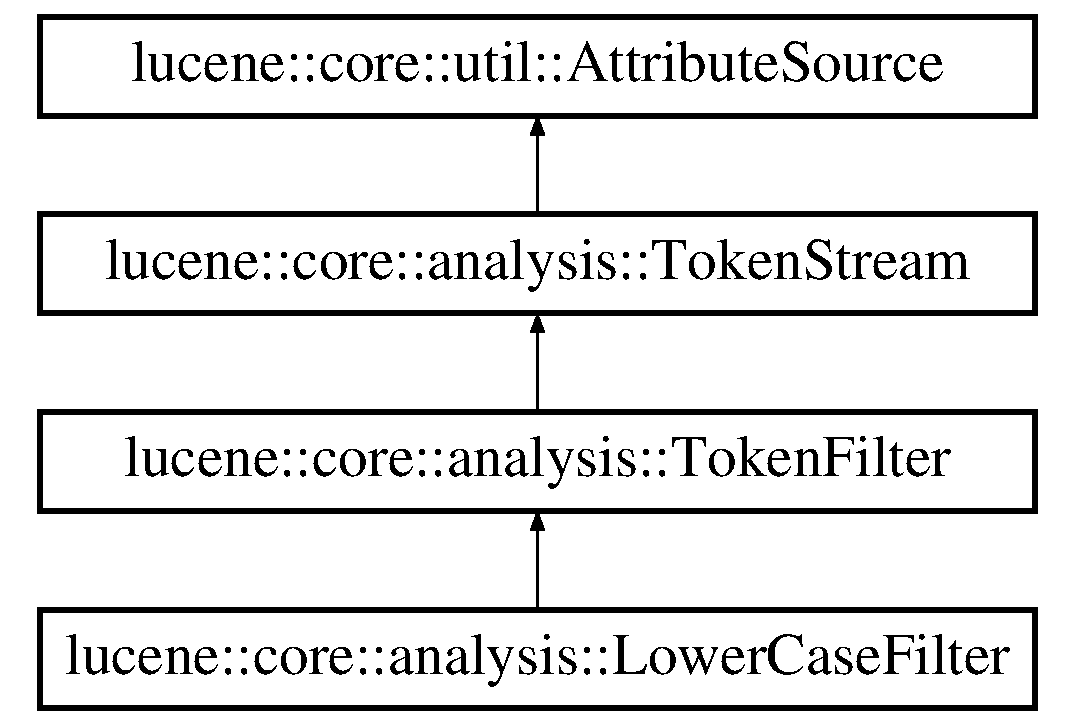
\includegraphics[height=4.000000cm]{classlucene_1_1core_1_1analysis_1_1LowerCaseFilter}
\end{center}
\end{figure}
\subsection*{Public Member Functions}
\begin{DoxyCompactItemize}
\item 
\mbox{\hyperlink{classlucene_1_1core_1_1analysis_1_1LowerCaseFilter_adc40b1a46dae685f8fded193589a8564}{Lower\+Case\+Filter}} (std\+::shared\+\_\+ptr$<$ \mbox{\hyperlink{classlucene_1_1core_1_1analysis_1_1TokenStream}{Token\+Stream}} $>$ in)
\item 
\mbox{\hyperlink{classlucene_1_1core_1_1analysis_1_1LowerCaseFilter_a9c099f0524d658bf260086b572831233}{Lower\+Case\+Filter}} (\mbox{\hyperlink{classlucene_1_1core_1_1analysis_1_1TokenStream}{Token\+Stream}} $\ast$in)
\item 
virtual \mbox{\hyperlink{classlucene_1_1core_1_1analysis_1_1LowerCaseFilter_a0f7565bddace8d24ef778bc34bb4eeb4}{$\sim$\+Lower\+Case\+Filter}} ()
\item 
bool \mbox{\hyperlink{classlucene_1_1core_1_1analysis_1_1LowerCaseFilter_a0e32bf7c330bccfb7ad3c68a374683a7}{Increment\+Token}} () override
\end{DoxyCompactItemize}
\subsection*{Private Attributes}
\begin{DoxyCompactItemize}
\item 
std\+::shared\+\_\+ptr$<$ \mbox{\hyperlink{classlucene_1_1core_1_1analysis_1_1tokenattributes_1_1CharTermAttribute}{tokenattributes\+::\+Char\+Term\+Attribute}} $>$ \mbox{\hyperlink{classlucene_1_1core_1_1analysis_1_1LowerCaseFilter_a0c5ad49e8254ea03353d3f02f3529b20}{term\+\_\+att}}
\end{DoxyCompactItemize}
\subsection*{Additional Inherited Members}


\subsection{Constructor \& Destructor Documentation}
\mbox{\Hypertarget{classlucene_1_1core_1_1analysis_1_1LowerCaseFilter_adc40b1a46dae685f8fded193589a8564}\label{classlucene_1_1core_1_1analysis_1_1LowerCaseFilter_adc40b1a46dae685f8fded193589a8564}} 
\index{lucene\+::core\+::analysis\+::\+Lower\+Case\+Filter@{lucene\+::core\+::analysis\+::\+Lower\+Case\+Filter}!Lower\+Case\+Filter@{Lower\+Case\+Filter}}
\index{Lower\+Case\+Filter@{Lower\+Case\+Filter}!lucene\+::core\+::analysis\+::\+Lower\+Case\+Filter@{lucene\+::core\+::analysis\+::\+Lower\+Case\+Filter}}
\subsubsection{\texorpdfstring{Lower\+Case\+Filter()}{LowerCaseFilter()}\hspace{0.1cm}{\footnotesize\ttfamily [1/2]}}
{\footnotesize\ttfamily lucene\+::core\+::analysis\+::\+Lower\+Case\+Filter\+::\+Lower\+Case\+Filter (\begin{DoxyParamCaption}\item[{std\+::shared\+\_\+ptr$<$ \mbox{\hyperlink{classlucene_1_1core_1_1analysis_1_1TokenStream}{Token\+Stream}} $>$}]{in }\end{DoxyParamCaption})\hspace{0.3cm}{\ttfamily [explicit]}}

\mbox{\Hypertarget{classlucene_1_1core_1_1analysis_1_1LowerCaseFilter_a9c099f0524d658bf260086b572831233}\label{classlucene_1_1core_1_1analysis_1_1LowerCaseFilter_a9c099f0524d658bf260086b572831233}} 
\index{lucene\+::core\+::analysis\+::\+Lower\+Case\+Filter@{lucene\+::core\+::analysis\+::\+Lower\+Case\+Filter}!Lower\+Case\+Filter@{Lower\+Case\+Filter}}
\index{Lower\+Case\+Filter@{Lower\+Case\+Filter}!lucene\+::core\+::analysis\+::\+Lower\+Case\+Filter@{lucene\+::core\+::analysis\+::\+Lower\+Case\+Filter}}
\subsubsection{\texorpdfstring{Lower\+Case\+Filter()}{LowerCaseFilter()}\hspace{0.1cm}{\footnotesize\ttfamily [2/2]}}
{\footnotesize\ttfamily Lower\+Case\+Filter\+::\+Lower\+Case\+Filter (\begin{DoxyParamCaption}\item[{\mbox{\hyperlink{classlucene_1_1core_1_1analysis_1_1TokenStream}{Token\+Stream}} $\ast$}]{in }\end{DoxyParamCaption})\hspace{0.3cm}{\ttfamily [explicit]}}

\mbox{\hyperlink{classlucene_1_1core_1_1analysis_1_1LowerCaseFilter}{Lower\+Case\+Filter}} \mbox{\Hypertarget{classlucene_1_1core_1_1analysis_1_1LowerCaseFilter_a0f7565bddace8d24ef778bc34bb4eeb4}\label{classlucene_1_1core_1_1analysis_1_1LowerCaseFilter_a0f7565bddace8d24ef778bc34bb4eeb4}} 
\index{lucene\+::core\+::analysis\+::\+Lower\+Case\+Filter@{lucene\+::core\+::analysis\+::\+Lower\+Case\+Filter}!````~Lower\+Case\+Filter@{$\sim$\+Lower\+Case\+Filter}}
\index{````~Lower\+Case\+Filter@{$\sim$\+Lower\+Case\+Filter}!lucene\+::core\+::analysis\+::\+Lower\+Case\+Filter@{lucene\+::core\+::analysis\+::\+Lower\+Case\+Filter}}
\subsubsection{\texorpdfstring{$\sim$\+Lower\+Case\+Filter()}{~LowerCaseFilter()}}
{\footnotesize\ttfamily Lower\+Case\+Filter\+::$\sim$\+Lower\+Case\+Filter (\begin{DoxyParamCaption}{ }\end{DoxyParamCaption})\hspace{0.3cm}{\ttfamily [virtual]}}



\subsection{Member Function Documentation}
\mbox{\Hypertarget{classlucene_1_1core_1_1analysis_1_1LowerCaseFilter_a0e32bf7c330bccfb7ad3c68a374683a7}\label{classlucene_1_1core_1_1analysis_1_1LowerCaseFilter_a0e32bf7c330bccfb7ad3c68a374683a7}} 
\index{lucene\+::core\+::analysis\+::\+Lower\+Case\+Filter@{lucene\+::core\+::analysis\+::\+Lower\+Case\+Filter}!Increment\+Token@{Increment\+Token}}
\index{Increment\+Token@{Increment\+Token}!lucene\+::core\+::analysis\+::\+Lower\+Case\+Filter@{lucene\+::core\+::analysis\+::\+Lower\+Case\+Filter}}
\subsubsection{\texorpdfstring{Increment\+Token()}{IncrementToken()}}
{\footnotesize\ttfamily bool Lower\+Case\+Filter\+::\+Increment\+Token (\begin{DoxyParamCaption}{ }\end{DoxyParamCaption})\hspace{0.3cm}{\ttfamily [override]}, {\ttfamily [virtual]}}



Implements \mbox{\hyperlink{classlucene_1_1core_1_1analysis_1_1TokenStream_a614d4ea24a354d6f4354b4941b5124e2}{lucene\+::core\+::analysis\+::\+Token\+Stream}}.



\subsection{Member Data Documentation}
\mbox{\Hypertarget{classlucene_1_1core_1_1analysis_1_1LowerCaseFilter_a0c5ad49e8254ea03353d3f02f3529b20}\label{classlucene_1_1core_1_1analysis_1_1LowerCaseFilter_a0c5ad49e8254ea03353d3f02f3529b20}} 
\index{lucene\+::core\+::analysis\+::\+Lower\+Case\+Filter@{lucene\+::core\+::analysis\+::\+Lower\+Case\+Filter}!term\+\_\+att@{term\+\_\+att}}
\index{term\+\_\+att@{term\+\_\+att}!lucene\+::core\+::analysis\+::\+Lower\+Case\+Filter@{lucene\+::core\+::analysis\+::\+Lower\+Case\+Filter}}
\subsubsection{\texorpdfstring{term\+\_\+att}{term\_att}}
{\footnotesize\ttfamily std\+::shared\+\_\+ptr$<$\mbox{\hyperlink{classlucene_1_1core_1_1analysis_1_1tokenattributes_1_1CharTermAttribute}{tokenattributes\+::\+Char\+Term\+Attribute}}$>$ lucene\+::core\+::analysis\+::\+Lower\+Case\+Filter\+::term\+\_\+att\hspace{0.3cm}{\ttfamily [private]}}



The documentation for this class was generated from the following files\+:\begin{DoxyCompactItemize}
\item 
Analysis/\mbox{\hyperlink{TokenStream_8h}{Token\+Stream.\+h}}\item 
Analysis/\mbox{\hyperlink{TokenStream_8cpp}{Token\+Stream.\+cpp}}\end{DoxyCompactItemize}

\hypertarget{classNaiveWhiteSpaceTokenizer}{}\section{Naive\+White\+Space\+Tokenizer Class Reference}
\label{classNaiveWhiteSpaceTokenizer}\index{Naive\+White\+Space\+Tokenizer@{Naive\+White\+Space\+Tokenizer}}
Inheritance diagram for Naive\+White\+Space\+Tokenizer\+:\begin{figure}[H]
\begin{center}
\leavevmode
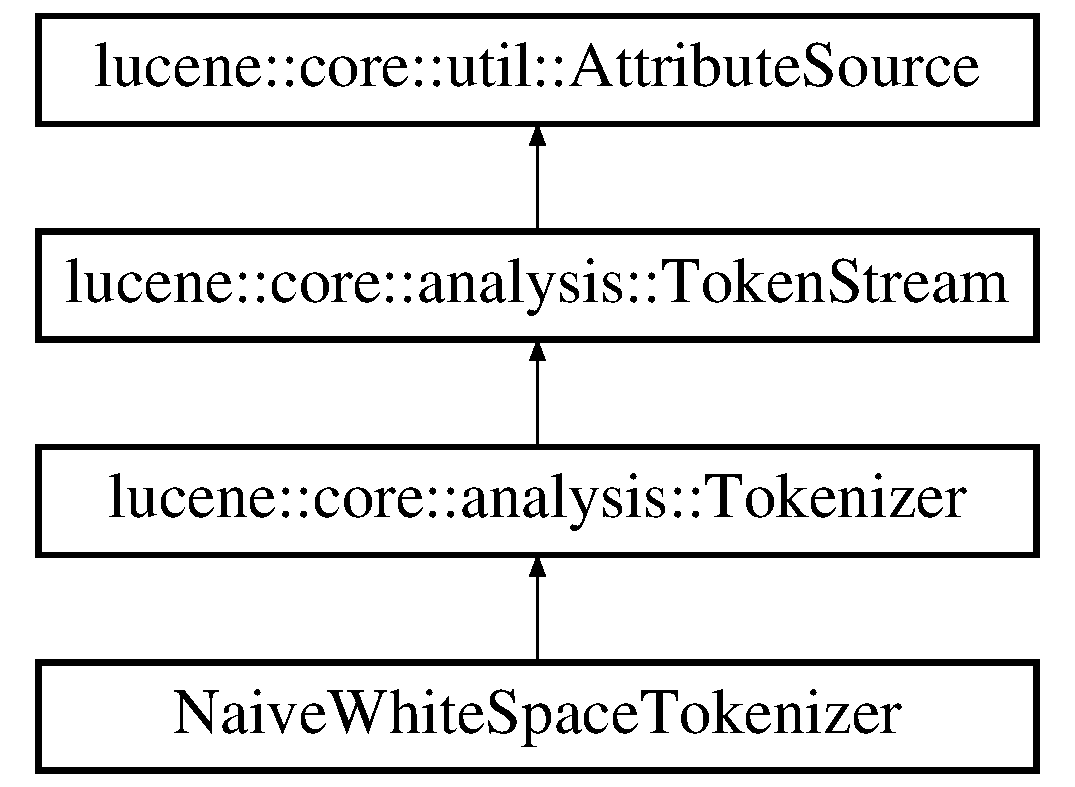
\includegraphics[height=4.000000cm]{classNaiveWhiteSpaceTokenizer}
\end{center}
\end{figure}
\subsection*{Public Member Functions}
\begin{DoxyCompactItemize}
\item 
\mbox{\hyperlink{classNaiveWhiteSpaceTokenizer_a4364bb2206efa47c4ea1cb9eb421d3ec}{Naive\+White\+Space\+Tokenizer}} ()
\item 
void \mbox{\hyperlink{classNaiveWhiteSpaceTokenizer_aa532e6a3e2fa6a9ebb90a4324179a30f}{Reset}} ()
\item 
void \mbox{\hyperlink{classNaiveWhiteSpaceTokenizer_a4c4f4debc08aa3e05b07b782144b5ae6}{End}} ()
\item 
bool \mbox{\hyperlink{classNaiveWhiteSpaceTokenizer_aa1dcc35eedacdb6107441cb9010d60b0}{Increment\+Token}} ()
\end{DoxyCompactItemize}
\subsection*{Public Attributes}
\begin{DoxyCompactItemize}
\item 
std\+::shared\+\_\+ptr$<$ \mbox{\hyperlink{classlucene_1_1core_1_1analysis_1_1tokenattributes_1_1CharTermAttribute}{Char\+Term\+Attribute}} $>$ \mbox{\hyperlink{classNaiveWhiteSpaceTokenizer_ad2b2c7263641059662c19db8a3da72a9}{term\+\_\+att}}
\item 
std\+::shared\+\_\+ptr$<$ \mbox{\hyperlink{classlucene_1_1core_1_1analysis_1_1tokenattributes_1_1OffsetAttribute}{Offset\+Attribute}} $>$ \mbox{\hyperlink{classNaiveWhiteSpaceTokenizer_a45e026472fc925608372e2881d1db2f2}{offset\+\_\+att}}
\item 
uint32\+\_\+t \mbox{\hyperlink{classNaiveWhiteSpaceTokenizer_aa655cc24b8bb85dfedbbb0b42a50db92}{index}}
\item 
uint32\+\_\+t \mbox{\hyperlink{classNaiveWhiteSpaceTokenizer_a94597a26813f5ac60aa3825bf57c20d8}{start\+\_\+offset}}
\item 
uint32\+\_\+t \mbox{\hyperlink{classNaiveWhiteSpaceTokenizer_ae68186bbc8f2a7f32d5c3c2f90014d7f}{end\+\_\+offset}}
\item 
std\+::string \mbox{\hyperlink{classNaiveWhiteSpaceTokenizer_a4d32b68e050394299ec7bfc6eddf7fd5}{line}}
\end{DoxyCompactItemize}
\subsection*{Additional Inherited Members}


\subsection{Constructor \& Destructor Documentation}
\mbox{\Hypertarget{classNaiveWhiteSpaceTokenizer_a4364bb2206efa47c4ea1cb9eb421d3ec}\label{classNaiveWhiteSpaceTokenizer_a4364bb2206efa47c4ea1cb9eb421d3ec}} 
\index{Naive\+White\+Space\+Tokenizer@{Naive\+White\+Space\+Tokenizer}!Naive\+White\+Space\+Tokenizer@{Naive\+White\+Space\+Tokenizer}}
\index{Naive\+White\+Space\+Tokenizer@{Naive\+White\+Space\+Tokenizer}!Naive\+White\+Space\+Tokenizer@{Naive\+White\+Space\+Tokenizer}}
\subsubsection{\texorpdfstring{Naive\+White\+Space\+Tokenizer()}{NaiveWhiteSpaceTokenizer()}}
{\footnotesize\ttfamily Naive\+White\+Space\+Tokenizer\+::\+Naive\+White\+Space\+Tokenizer (\begin{DoxyParamCaption}{ }\end{DoxyParamCaption})\hspace{0.3cm}{\ttfamily [inline]}}



\subsection{Member Function Documentation}
\mbox{\Hypertarget{classNaiveWhiteSpaceTokenizer_a4c4f4debc08aa3e05b07b782144b5ae6}\label{classNaiveWhiteSpaceTokenizer_a4c4f4debc08aa3e05b07b782144b5ae6}} 
\index{Naive\+White\+Space\+Tokenizer@{Naive\+White\+Space\+Tokenizer}!End@{End}}
\index{End@{End}!Naive\+White\+Space\+Tokenizer@{Naive\+White\+Space\+Tokenizer}}
\subsubsection{\texorpdfstring{End()}{End()}}
{\footnotesize\ttfamily void Naive\+White\+Space\+Tokenizer\+::\+End (\begin{DoxyParamCaption}{ }\end{DoxyParamCaption})\hspace{0.3cm}{\ttfamily [inline]}, {\ttfamily [virtual]}}



Reimplemented from \mbox{\hyperlink{classlucene_1_1core_1_1analysis_1_1TokenStream_a4693985ca7fb242412049a074027b8b5}{lucene\+::core\+::analysis\+::\+Token\+Stream}}.

\mbox{\Hypertarget{classNaiveWhiteSpaceTokenizer_aa1dcc35eedacdb6107441cb9010d60b0}\label{classNaiveWhiteSpaceTokenizer_aa1dcc35eedacdb6107441cb9010d60b0}} 
\index{Naive\+White\+Space\+Tokenizer@{Naive\+White\+Space\+Tokenizer}!Increment\+Token@{Increment\+Token}}
\index{Increment\+Token@{Increment\+Token}!Naive\+White\+Space\+Tokenizer@{Naive\+White\+Space\+Tokenizer}}
\subsubsection{\texorpdfstring{Increment\+Token()}{IncrementToken()}}
{\footnotesize\ttfamily bool Naive\+White\+Space\+Tokenizer\+::\+Increment\+Token (\begin{DoxyParamCaption}{ }\end{DoxyParamCaption})\hspace{0.3cm}{\ttfamily [inline]}, {\ttfamily [virtual]}}



Implements \mbox{\hyperlink{classlucene_1_1core_1_1analysis_1_1TokenStream_a614d4ea24a354d6f4354b4941b5124e2}{lucene\+::core\+::analysis\+::\+Token\+Stream}}.

\mbox{\Hypertarget{classNaiveWhiteSpaceTokenizer_aa532e6a3e2fa6a9ebb90a4324179a30f}\label{classNaiveWhiteSpaceTokenizer_aa532e6a3e2fa6a9ebb90a4324179a30f}} 
\index{Naive\+White\+Space\+Tokenizer@{Naive\+White\+Space\+Tokenizer}!Reset@{Reset}}
\index{Reset@{Reset}!Naive\+White\+Space\+Tokenizer@{Naive\+White\+Space\+Tokenizer}}
\subsubsection{\texorpdfstring{Reset()}{Reset()}}
{\footnotesize\ttfamily void Naive\+White\+Space\+Tokenizer\+::\+Reset (\begin{DoxyParamCaption}{ }\end{DoxyParamCaption})\hspace{0.3cm}{\ttfamily [inline]}, {\ttfamily [virtual]}}



Implements \mbox{\hyperlink{classlucene_1_1core_1_1analysis_1_1TokenStream_ae24622f4bc0aeaf0bef924ff1661e023}{lucene\+::core\+::analysis\+::\+Token\+Stream}}.



\subsection{Member Data Documentation}
\mbox{\Hypertarget{classNaiveWhiteSpaceTokenizer_ae68186bbc8f2a7f32d5c3c2f90014d7f}\label{classNaiveWhiteSpaceTokenizer_ae68186bbc8f2a7f32d5c3c2f90014d7f}} 
\index{Naive\+White\+Space\+Tokenizer@{Naive\+White\+Space\+Tokenizer}!end\+\_\+offset@{end\+\_\+offset}}
\index{end\+\_\+offset@{end\+\_\+offset}!Naive\+White\+Space\+Tokenizer@{Naive\+White\+Space\+Tokenizer}}
\subsubsection{\texorpdfstring{end\+\_\+offset}{end\_offset}}
{\footnotesize\ttfamily uint32\+\_\+t Naive\+White\+Space\+Tokenizer\+::end\+\_\+offset}

\mbox{\Hypertarget{classNaiveWhiteSpaceTokenizer_aa655cc24b8bb85dfedbbb0b42a50db92}\label{classNaiveWhiteSpaceTokenizer_aa655cc24b8bb85dfedbbb0b42a50db92}} 
\index{Naive\+White\+Space\+Tokenizer@{Naive\+White\+Space\+Tokenizer}!index@{index}}
\index{index@{index}!Naive\+White\+Space\+Tokenizer@{Naive\+White\+Space\+Tokenizer}}
\subsubsection{\texorpdfstring{index}{index}}
{\footnotesize\ttfamily uint32\+\_\+t Naive\+White\+Space\+Tokenizer\+::index}

\mbox{\Hypertarget{classNaiveWhiteSpaceTokenizer_a4d32b68e050394299ec7bfc6eddf7fd5}\label{classNaiveWhiteSpaceTokenizer_a4d32b68e050394299ec7bfc6eddf7fd5}} 
\index{Naive\+White\+Space\+Tokenizer@{Naive\+White\+Space\+Tokenizer}!line@{line}}
\index{line@{line}!Naive\+White\+Space\+Tokenizer@{Naive\+White\+Space\+Tokenizer}}
\subsubsection{\texorpdfstring{line}{line}}
{\footnotesize\ttfamily std\+::string Naive\+White\+Space\+Tokenizer\+::line}

\mbox{\Hypertarget{classNaiveWhiteSpaceTokenizer_a45e026472fc925608372e2881d1db2f2}\label{classNaiveWhiteSpaceTokenizer_a45e026472fc925608372e2881d1db2f2}} 
\index{Naive\+White\+Space\+Tokenizer@{Naive\+White\+Space\+Tokenizer}!offset\+\_\+att@{offset\+\_\+att}}
\index{offset\+\_\+att@{offset\+\_\+att}!Naive\+White\+Space\+Tokenizer@{Naive\+White\+Space\+Tokenizer}}
\subsubsection{\texorpdfstring{offset\+\_\+att}{offset\_att}}
{\footnotesize\ttfamily std\+::shared\+\_\+ptr$<$\mbox{\hyperlink{classlucene_1_1core_1_1analysis_1_1tokenattributes_1_1OffsetAttribute}{Offset\+Attribute}}$>$ Naive\+White\+Space\+Tokenizer\+::offset\+\_\+att}

\mbox{\Hypertarget{classNaiveWhiteSpaceTokenizer_a94597a26813f5ac60aa3825bf57c20d8}\label{classNaiveWhiteSpaceTokenizer_a94597a26813f5ac60aa3825bf57c20d8}} 
\index{Naive\+White\+Space\+Tokenizer@{Naive\+White\+Space\+Tokenizer}!start\+\_\+offset@{start\+\_\+offset}}
\index{start\+\_\+offset@{start\+\_\+offset}!Naive\+White\+Space\+Tokenizer@{Naive\+White\+Space\+Tokenizer}}
\subsubsection{\texorpdfstring{start\+\_\+offset}{start\_offset}}
{\footnotesize\ttfamily uint32\+\_\+t Naive\+White\+Space\+Tokenizer\+::start\+\_\+offset}

\mbox{\Hypertarget{classNaiveWhiteSpaceTokenizer_ad2b2c7263641059662c19db8a3da72a9}\label{classNaiveWhiteSpaceTokenizer_ad2b2c7263641059662c19db8a3da72a9}} 
\index{Naive\+White\+Space\+Tokenizer@{Naive\+White\+Space\+Tokenizer}!term\+\_\+att@{term\+\_\+att}}
\index{term\+\_\+att@{term\+\_\+att}!Naive\+White\+Space\+Tokenizer@{Naive\+White\+Space\+Tokenizer}}
\subsubsection{\texorpdfstring{term\+\_\+att}{term\_att}}
{\footnotesize\ttfamily std\+::shared\+\_\+ptr$<$\mbox{\hyperlink{classlucene_1_1core_1_1analysis_1_1tokenattributes_1_1CharTermAttribute}{Char\+Term\+Attribute}}$>$ Naive\+White\+Space\+Tokenizer\+::term\+\_\+att}



The documentation for this class was generated from the following file\+:\begin{DoxyCompactItemize}
\item 
Analysis/tests/\mbox{\hyperlink{TokenStreamTests_8cpp}{Token\+Stream\+Tests.\+cpp}}\end{DoxyCompactItemize}

\hypertarget{classlucene_1_1core_1_1analysis_1_1tokenattributes_1_1OffsetAttribute}{}\section{lucene\+:\+:core\+:\+:analysis\+:\+:tokenattributes\+:\+:Offset\+Attribute Class Reference}
\label{classlucene_1_1core_1_1analysis_1_1tokenattributes_1_1OffsetAttribute}\index{lucene\+::core\+::analysis\+::tokenattributes\+::\+Offset\+Attribute@{lucene\+::core\+::analysis\+::tokenattributes\+::\+Offset\+Attribute}}


{\ttfamily \#include $<$Attribute.\+h$>$}

Inheritance diagram for lucene\+:\+:core\+:\+:analysis\+:\+:tokenattributes\+:\+:Offset\+Attribute\+:\begin{figure}[H]
\begin{center}
\leavevmode
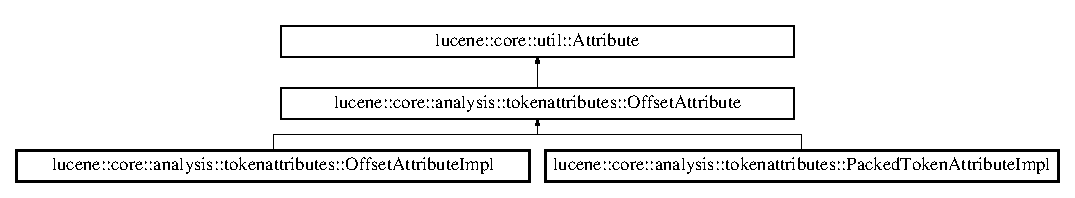
\includegraphics[height=2.210526cm]{classlucene_1_1core_1_1analysis_1_1tokenattributes_1_1OffsetAttribute}
\end{center}
\end{figure}
\subsection*{Public Member Functions}
\begin{DoxyCompactItemize}
\item 
virtual \mbox{\hyperlink{classlucene_1_1core_1_1analysis_1_1tokenattributes_1_1OffsetAttribute_aae91ff2e429a7f882d00b64a01b1f326}{$\sim$\+Offset\+Attribute}} ()
\item 
virtual uint32\+\_\+t \mbox{\hyperlink{classlucene_1_1core_1_1analysis_1_1tokenattributes_1_1OffsetAttribute_af841d190a7900a5b6a00f0a9f4ae7e43}{Start\+Offset}} ()=0
\item 
virtual void \mbox{\hyperlink{classlucene_1_1core_1_1analysis_1_1tokenattributes_1_1OffsetAttribute_aa0d076ac2e7c5af86668fbbeb8e26170}{Set\+Offset}} (const uint32\+\_\+t start\+\_\+offset, const uint32\+\_\+t end\+\_\+offset)=0
\item 
virtual uint32\+\_\+t \mbox{\hyperlink{classlucene_1_1core_1_1analysis_1_1tokenattributes_1_1OffsetAttribute_ada281ff6240e1a0fecf57707329ec974}{End\+Offset}} ()=0
\end{DoxyCompactItemize}
\subsection*{Additional Inherited Members}


\subsection{Constructor \& Destructor Documentation}
\mbox{\Hypertarget{classlucene_1_1core_1_1analysis_1_1tokenattributes_1_1OffsetAttribute_aae91ff2e429a7f882d00b64a01b1f326}\label{classlucene_1_1core_1_1analysis_1_1tokenattributes_1_1OffsetAttribute_aae91ff2e429a7f882d00b64a01b1f326}} 
\index{lucene\+::core\+::analysis\+::tokenattributes\+::\+Offset\+Attribute@{lucene\+::core\+::analysis\+::tokenattributes\+::\+Offset\+Attribute}!````~Offset\+Attribute@{$\sim$\+Offset\+Attribute}}
\index{````~Offset\+Attribute@{$\sim$\+Offset\+Attribute}!lucene\+::core\+::analysis\+::tokenattributes\+::\+Offset\+Attribute@{lucene\+::core\+::analysis\+::tokenattributes\+::\+Offset\+Attribute}}
\subsubsection{\texorpdfstring{$\sim$\+Offset\+Attribute()}{~OffsetAttribute()}}
{\footnotesize\ttfamily virtual lucene\+::core\+::analysis\+::tokenattributes\+::\+Offset\+Attribute\+::$\sim$\+Offset\+Attribute (\begin{DoxyParamCaption}{ }\end{DoxyParamCaption})\hspace{0.3cm}{\ttfamily [inline]}, {\ttfamily [virtual]}}



\subsection{Member Function Documentation}
\mbox{\Hypertarget{classlucene_1_1core_1_1analysis_1_1tokenattributes_1_1OffsetAttribute_ada281ff6240e1a0fecf57707329ec974}\label{classlucene_1_1core_1_1analysis_1_1tokenattributes_1_1OffsetAttribute_ada281ff6240e1a0fecf57707329ec974}} 
\index{lucene\+::core\+::analysis\+::tokenattributes\+::\+Offset\+Attribute@{lucene\+::core\+::analysis\+::tokenattributes\+::\+Offset\+Attribute}!End\+Offset@{End\+Offset}}
\index{End\+Offset@{End\+Offset}!lucene\+::core\+::analysis\+::tokenattributes\+::\+Offset\+Attribute@{lucene\+::core\+::analysis\+::tokenattributes\+::\+Offset\+Attribute}}
\subsubsection{\texorpdfstring{End\+Offset()}{EndOffset()}}
{\footnotesize\ttfamily virtual uint32\+\_\+t lucene\+::core\+::analysis\+::tokenattributes\+::\+Offset\+Attribute\+::\+End\+Offset (\begin{DoxyParamCaption}{ }\end{DoxyParamCaption})\hspace{0.3cm}{\ttfamily [pure virtual]}}



Implemented in \mbox{\hyperlink{classlucene_1_1core_1_1analysis_1_1tokenattributes_1_1PackedTokenAttributeImpl_ae6210d544884be562c186a040d91157f}{lucene\+::core\+::analysis\+::tokenattributes\+::\+Packed\+Token\+Attribute\+Impl}}, and \mbox{\hyperlink{classlucene_1_1core_1_1analysis_1_1tokenattributes_1_1OffsetAttributeImpl_a1e70ec558f605ea2313e41ba5c64e379}{lucene\+::core\+::analysis\+::tokenattributes\+::\+Offset\+Attribute\+Impl}}.

\mbox{\Hypertarget{classlucene_1_1core_1_1analysis_1_1tokenattributes_1_1OffsetAttribute_aa0d076ac2e7c5af86668fbbeb8e26170}\label{classlucene_1_1core_1_1analysis_1_1tokenattributes_1_1OffsetAttribute_aa0d076ac2e7c5af86668fbbeb8e26170}} 
\index{lucene\+::core\+::analysis\+::tokenattributes\+::\+Offset\+Attribute@{lucene\+::core\+::analysis\+::tokenattributes\+::\+Offset\+Attribute}!Set\+Offset@{Set\+Offset}}
\index{Set\+Offset@{Set\+Offset}!lucene\+::core\+::analysis\+::tokenattributes\+::\+Offset\+Attribute@{lucene\+::core\+::analysis\+::tokenattributes\+::\+Offset\+Attribute}}
\subsubsection{\texorpdfstring{Set\+Offset()}{SetOffset()}}
{\footnotesize\ttfamily virtual void lucene\+::core\+::analysis\+::tokenattributes\+::\+Offset\+Attribute\+::\+Set\+Offset (\begin{DoxyParamCaption}\item[{const uint32\+\_\+t}]{start\+\_\+offset,  }\item[{const uint32\+\_\+t}]{end\+\_\+offset }\end{DoxyParamCaption})\hspace{0.3cm}{\ttfamily [pure virtual]}}



Implemented in \mbox{\hyperlink{classlucene_1_1core_1_1analysis_1_1tokenattributes_1_1PackedTokenAttributeImpl_aa17ed401f2b9f6bd773291de1d02bb35}{lucene\+::core\+::analysis\+::tokenattributes\+::\+Packed\+Token\+Attribute\+Impl}}, and \mbox{\hyperlink{classlucene_1_1core_1_1analysis_1_1tokenattributes_1_1OffsetAttributeImpl_ab554b85bf6d64ce023c0634b3883c803}{lucene\+::core\+::analysis\+::tokenattributes\+::\+Offset\+Attribute\+Impl}}.

\mbox{\Hypertarget{classlucene_1_1core_1_1analysis_1_1tokenattributes_1_1OffsetAttribute_af841d190a7900a5b6a00f0a9f4ae7e43}\label{classlucene_1_1core_1_1analysis_1_1tokenattributes_1_1OffsetAttribute_af841d190a7900a5b6a00f0a9f4ae7e43}} 
\index{lucene\+::core\+::analysis\+::tokenattributes\+::\+Offset\+Attribute@{lucene\+::core\+::analysis\+::tokenattributes\+::\+Offset\+Attribute}!Start\+Offset@{Start\+Offset}}
\index{Start\+Offset@{Start\+Offset}!lucene\+::core\+::analysis\+::tokenattributes\+::\+Offset\+Attribute@{lucene\+::core\+::analysis\+::tokenattributes\+::\+Offset\+Attribute}}
\subsubsection{\texorpdfstring{Start\+Offset()}{StartOffset()}}
{\footnotesize\ttfamily virtual uint32\+\_\+t lucene\+::core\+::analysis\+::tokenattributes\+::\+Offset\+Attribute\+::\+Start\+Offset (\begin{DoxyParamCaption}{ }\end{DoxyParamCaption})\hspace{0.3cm}{\ttfamily [pure virtual]}}



Implemented in \mbox{\hyperlink{classlucene_1_1core_1_1analysis_1_1tokenattributes_1_1PackedTokenAttributeImpl_aea927563f771802e2ea6356814b53c17}{lucene\+::core\+::analysis\+::tokenattributes\+::\+Packed\+Token\+Attribute\+Impl}}, and \mbox{\hyperlink{classlucene_1_1core_1_1analysis_1_1tokenattributes_1_1OffsetAttributeImpl_afe05dd1af07cc98ff4baceb531ae5f0a}{lucene\+::core\+::analysis\+::tokenattributes\+::\+Offset\+Attribute\+Impl}}.



The documentation for this class was generated from the following file\+:\begin{DoxyCompactItemize}
\item 
Analysis/\mbox{\hyperlink{Analysis_2Attribute_8h}{Attribute.\+h}}\end{DoxyCompactItemize}

\hypertarget{classlucene_1_1core_1_1analysis_1_1tokenattributes_1_1OffsetAttributeImpl}{}\section{lucene\+:\+:core\+:\+:analysis\+:\+:tokenattributes\+:\+:Offset\+Attribute\+Impl Class Reference}
\label{classlucene_1_1core_1_1analysis_1_1tokenattributes_1_1OffsetAttributeImpl}\index{lucene\+::core\+::analysis\+::tokenattributes\+::\+Offset\+Attribute\+Impl@{lucene\+::core\+::analysis\+::tokenattributes\+::\+Offset\+Attribute\+Impl}}


{\ttfamily \#include $<$Attribute\+Impl.\+h$>$}

Inheritance diagram for lucene\+:\+:core\+:\+:analysis\+:\+:tokenattributes\+:\+:Offset\+Attribute\+Impl\+:\begin{figure}[H]
\begin{center}
\leavevmode
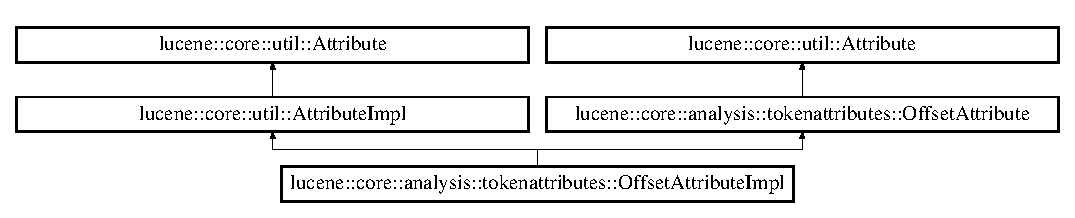
\includegraphics[height=2.485207cm]{classlucene_1_1core_1_1analysis_1_1tokenattributes_1_1OffsetAttributeImpl}
\end{center}
\end{figure}
\subsection*{Public Member Functions}
\begin{DoxyCompactItemize}
\item 
\mbox{\hyperlink{classlucene_1_1core_1_1analysis_1_1tokenattributes_1_1OffsetAttributeImpl_a424f18384e62360c38c1cd3e797dc80c}{Offset\+Attribute\+Impl}} ()
\item 
\mbox{\hyperlink{classlucene_1_1core_1_1analysis_1_1tokenattributes_1_1OffsetAttributeImpl_a1b302380db18cbe111ddc892b3b04841}{Offset\+Attribute\+Impl}} (\mbox{\hyperlink{ZlibCrc32_8h_a2c212835823e3c54a8ab6d95c652660e}{const}} \mbox{\hyperlink{classlucene_1_1core_1_1analysis_1_1tokenattributes_1_1OffsetAttributeImpl}{Offset\+Attribute\+Impl}} \&other)
\item 
virtual \mbox{\hyperlink{classlucene_1_1core_1_1analysis_1_1tokenattributes_1_1OffsetAttributeImpl_a6de20d33c5e4aed543d2386ccb3cef69}{$\sim$\+Offset\+Attribute\+Impl}} ()
\item 
uint32\+\_\+t \mbox{\hyperlink{classlucene_1_1core_1_1analysis_1_1tokenattributes_1_1OffsetAttributeImpl_afe05dd1af07cc98ff4baceb531ae5f0a}{Start\+Offset}} () override
\item 
void \mbox{\hyperlink{classlucene_1_1core_1_1analysis_1_1tokenattributes_1_1OffsetAttributeImpl_ab554b85bf6d64ce023c0634b3883c803}{Set\+Offset}} (\mbox{\hyperlink{ZlibCrc32_8h_a2c212835823e3c54a8ab6d95c652660e}{const}} uint32\+\_\+t \mbox{\hyperlink{classlucene_1_1core_1_1analysis_1_1tokenattributes_1_1OffsetAttributeImpl_a1e2b8c747f3f0216a9044b9fd61ea843}{start\+\_\+offset}}, \mbox{\hyperlink{ZlibCrc32_8h_a2c212835823e3c54a8ab6d95c652660e}{const}} uint32\+\_\+t \mbox{\hyperlink{classlucene_1_1core_1_1analysis_1_1tokenattributes_1_1OffsetAttributeImpl_a2e25d7e34687e7d39baaaf88636238c7}{end\+\_\+offset}}) override
\item 
uint32\+\_\+t \mbox{\hyperlink{classlucene_1_1core_1_1analysis_1_1tokenattributes_1_1OffsetAttributeImpl_a1e70ec558f605ea2313e41ba5c64e379}{End\+Offset}} () override
\item 
void \mbox{\hyperlink{classlucene_1_1core_1_1analysis_1_1tokenattributes_1_1OffsetAttributeImpl_ad7eb3a266863f7e14fbe1caa315c7151}{Reflect\+With}} (\mbox{\hyperlink{namespacelucene_1_1core_1_1util_a7dbb701adaed055f73fb95eec83da10a}{lucene\+::core\+::util\+::\+Attribute\+Reflector}} \&reflector) override
\item 
void \mbox{\hyperlink{classlucene_1_1core_1_1analysis_1_1tokenattributes_1_1OffsetAttributeImpl_af19f560600cc53e48c592aa6d9c48a91}{Clear}} () override
\item 
bool \mbox{\hyperlink{classlucene_1_1core_1_1analysis_1_1tokenattributes_1_1OffsetAttributeImpl_a3a7da0e72e05757a8e2c540fc639cca8}{operator==}} (\mbox{\hyperlink{ZlibCrc32_8h_a2c212835823e3c54a8ab6d95c652660e}{const}} \mbox{\hyperlink{classlucene_1_1core_1_1analysis_1_1tokenattributes_1_1OffsetAttributeImpl}{Offset\+Attribute\+Impl}} \&other) \mbox{\hyperlink{ZlibCrc32_8h_a2c212835823e3c54a8ab6d95c652660e}{const}}
\item 
std\+::vector$<$ std\+::type\+\_\+index $>$ \mbox{\hyperlink{classlucene_1_1core_1_1analysis_1_1tokenattributes_1_1OffsetAttributeImpl_ac2f3c035417acfc9056a900903f1d271}{Attributes}} () override
\item 
void \mbox{\hyperlink{classlucene_1_1core_1_1analysis_1_1tokenattributes_1_1OffsetAttributeImpl_a426d0cd75306c4ef7cec3c28e34c0029}{Shallow\+Copy\+To}} (\mbox{\hyperlink{classlucene_1_1core_1_1util_1_1AttributeImpl}{lucene\+::core\+::util\+::\+Attribute\+Impl}} \&attr\+\_\+impl) override
\item 
\mbox{\hyperlink{classlucene_1_1core_1_1analysis_1_1tokenattributes_1_1OffsetAttributeImpl}{Offset\+Attribute\+Impl}} \& \mbox{\hyperlink{classlucene_1_1core_1_1analysis_1_1tokenattributes_1_1OffsetAttributeImpl_ad5aee8c4731cfda2c9a1c7b7dbe4dc30}{operator=}} (\mbox{\hyperlink{ZlibCrc32_8h_a2c212835823e3c54a8ab6d95c652660e}{const}} \mbox{\hyperlink{classlucene_1_1core_1_1util_1_1AttributeImpl}{lucene\+::core\+::util\+::\+Attribute\+Impl}} \&other)
\item 
\mbox{\hyperlink{classlucene_1_1core_1_1analysis_1_1tokenattributes_1_1OffsetAttributeImpl}{Offset\+Attribute\+Impl}} \& \mbox{\hyperlink{classlucene_1_1core_1_1analysis_1_1tokenattributes_1_1OffsetAttributeImpl_ab26c5fb656b41c725bb7207da7877c4a}{operator=}} (\mbox{\hyperlink{ZlibCrc32_8h_a2c212835823e3c54a8ab6d95c652660e}{const}} \mbox{\hyperlink{classlucene_1_1core_1_1analysis_1_1tokenattributes_1_1OffsetAttributeImpl}{Offset\+Attribute\+Impl}} \&other)
\item 
\mbox{\hyperlink{classlucene_1_1core_1_1util_1_1AttributeImpl}{lucene\+::core\+::util\+::\+Attribute\+Impl}} $\ast$ \mbox{\hyperlink{classlucene_1_1core_1_1analysis_1_1tokenattributes_1_1OffsetAttributeImpl_a4cae4e770c4ce5184ae4530edde06bae}{Clone}} () override
\end{DoxyCompactItemize}
\subsection*{Private Attributes}
\begin{DoxyCompactItemize}
\item 
uint32\+\_\+t \mbox{\hyperlink{classlucene_1_1core_1_1analysis_1_1tokenattributes_1_1OffsetAttributeImpl_a1e2b8c747f3f0216a9044b9fd61ea843}{start\+\_\+offset}}
\item 
uint32\+\_\+t \mbox{\hyperlink{classlucene_1_1core_1_1analysis_1_1tokenattributes_1_1OffsetAttributeImpl_a2e25d7e34687e7d39baaaf88636238c7}{end\+\_\+offset}}
\end{DoxyCompactItemize}
\subsection*{Additional Inherited Members}


\subsection{Constructor \& Destructor Documentation}
\mbox{\Hypertarget{classlucene_1_1core_1_1analysis_1_1tokenattributes_1_1OffsetAttributeImpl_a424f18384e62360c38c1cd3e797dc80c}\label{classlucene_1_1core_1_1analysis_1_1tokenattributes_1_1OffsetAttributeImpl_a424f18384e62360c38c1cd3e797dc80c}} 
\index{lucene\+::core\+::analysis\+::tokenattributes\+::\+Offset\+Attribute\+Impl@{lucene\+::core\+::analysis\+::tokenattributes\+::\+Offset\+Attribute\+Impl}!Offset\+Attribute\+Impl@{Offset\+Attribute\+Impl}}
\index{Offset\+Attribute\+Impl@{Offset\+Attribute\+Impl}!lucene\+::core\+::analysis\+::tokenattributes\+::\+Offset\+Attribute\+Impl@{lucene\+::core\+::analysis\+::tokenattributes\+::\+Offset\+Attribute\+Impl}}
\subsubsection{\texorpdfstring{Offset\+Attribute\+Impl()}{OffsetAttributeImpl()}\hspace{0.1cm}{\footnotesize\ttfamily [1/2]}}
{\footnotesize\ttfamily Offset\+Attribute\+Impl\+::\+Offset\+Attribute\+Impl (\begin{DoxyParamCaption}{ }\end{DoxyParamCaption})}

\mbox{\hyperlink{classlucene_1_1core_1_1analysis_1_1tokenattributes_1_1OffsetAttributeImpl}{Offset\+Attribute\+Impl}} \mbox{\Hypertarget{classlucene_1_1core_1_1analysis_1_1tokenattributes_1_1OffsetAttributeImpl_a1b302380db18cbe111ddc892b3b04841}\label{classlucene_1_1core_1_1analysis_1_1tokenattributes_1_1OffsetAttributeImpl_a1b302380db18cbe111ddc892b3b04841}} 
\index{lucene\+::core\+::analysis\+::tokenattributes\+::\+Offset\+Attribute\+Impl@{lucene\+::core\+::analysis\+::tokenattributes\+::\+Offset\+Attribute\+Impl}!Offset\+Attribute\+Impl@{Offset\+Attribute\+Impl}}
\index{Offset\+Attribute\+Impl@{Offset\+Attribute\+Impl}!lucene\+::core\+::analysis\+::tokenattributes\+::\+Offset\+Attribute\+Impl@{lucene\+::core\+::analysis\+::tokenattributes\+::\+Offset\+Attribute\+Impl}}
\subsubsection{\texorpdfstring{Offset\+Attribute\+Impl()}{OffsetAttributeImpl()}\hspace{0.1cm}{\footnotesize\ttfamily [2/2]}}
{\footnotesize\ttfamily Offset\+Attribute\+Impl\+::\+Offset\+Attribute\+Impl (\begin{DoxyParamCaption}\item[{\mbox{\hyperlink{ZlibCrc32_8h_a2c212835823e3c54a8ab6d95c652660e}{const}} \mbox{\hyperlink{classlucene_1_1core_1_1analysis_1_1tokenattributes_1_1OffsetAttributeImpl}{Offset\+Attribute\+Impl}} \&}]{other }\end{DoxyParamCaption})}

\mbox{\Hypertarget{classlucene_1_1core_1_1analysis_1_1tokenattributes_1_1OffsetAttributeImpl_a6de20d33c5e4aed543d2386ccb3cef69}\label{classlucene_1_1core_1_1analysis_1_1tokenattributes_1_1OffsetAttributeImpl_a6de20d33c5e4aed543d2386ccb3cef69}} 
\index{lucene\+::core\+::analysis\+::tokenattributes\+::\+Offset\+Attribute\+Impl@{lucene\+::core\+::analysis\+::tokenattributes\+::\+Offset\+Attribute\+Impl}!````~Offset\+Attribute\+Impl@{$\sim$\+Offset\+Attribute\+Impl}}
\index{````~Offset\+Attribute\+Impl@{$\sim$\+Offset\+Attribute\+Impl}!lucene\+::core\+::analysis\+::tokenattributes\+::\+Offset\+Attribute\+Impl@{lucene\+::core\+::analysis\+::tokenattributes\+::\+Offset\+Attribute\+Impl}}
\subsubsection{\texorpdfstring{$\sim$\+Offset\+Attribute\+Impl()}{~OffsetAttributeImpl()}}
{\footnotesize\ttfamily Offset\+Attribute\+Impl\+::$\sim$\+Offset\+Attribute\+Impl (\begin{DoxyParamCaption}{ }\end{DoxyParamCaption})\hspace{0.3cm}{\ttfamily [virtual]}}



\subsection{Member Function Documentation}
\mbox{\Hypertarget{classlucene_1_1core_1_1analysis_1_1tokenattributes_1_1OffsetAttributeImpl_ac2f3c035417acfc9056a900903f1d271}\label{classlucene_1_1core_1_1analysis_1_1tokenattributes_1_1OffsetAttributeImpl_ac2f3c035417acfc9056a900903f1d271}} 
\index{lucene\+::core\+::analysis\+::tokenattributes\+::\+Offset\+Attribute\+Impl@{lucene\+::core\+::analysis\+::tokenattributes\+::\+Offset\+Attribute\+Impl}!Attributes@{Attributes}}
\index{Attributes@{Attributes}!lucene\+::core\+::analysis\+::tokenattributes\+::\+Offset\+Attribute\+Impl@{lucene\+::core\+::analysis\+::tokenattributes\+::\+Offset\+Attribute\+Impl}}
\subsubsection{\texorpdfstring{Attributes()}{Attributes()}}
{\footnotesize\ttfamily std\+::vector$<$ std\+::type\+\_\+index $>$ Offset\+Attribute\+Impl\+::\+Attributes (\begin{DoxyParamCaption}{ }\end{DoxyParamCaption})\hspace{0.3cm}{\ttfamily [override]}, {\ttfamily [virtual]}}



Implements \mbox{\hyperlink{classlucene_1_1core_1_1util_1_1AttributeImpl_ac0631e6a7a11044883bc97447716d7cc}{lucene\+::core\+::util\+::\+Attribute\+Impl}}.

\mbox{\Hypertarget{classlucene_1_1core_1_1analysis_1_1tokenattributes_1_1OffsetAttributeImpl_af19f560600cc53e48c592aa6d9c48a91}\label{classlucene_1_1core_1_1analysis_1_1tokenattributes_1_1OffsetAttributeImpl_af19f560600cc53e48c592aa6d9c48a91}} 
\index{lucene\+::core\+::analysis\+::tokenattributes\+::\+Offset\+Attribute\+Impl@{lucene\+::core\+::analysis\+::tokenattributes\+::\+Offset\+Attribute\+Impl}!Clear@{Clear}}
\index{Clear@{Clear}!lucene\+::core\+::analysis\+::tokenattributes\+::\+Offset\+Attribute\+Impl@{lucene\+::core\+::analysis\+::tokenattributes\+::\+Offset\+Attribute\+Impl}}
\subsubsection{\texorpdfstring{Clear()}{Clear()}}
{\footnotesize\ttfamily void Offset\+Attribute\+Impl\+::\+Clear (\begin{DoxyParamCaption}{ }\end{DoxyParamCaption})\hspace{0.3cm}{\ttfamily [override]}, {\ttfamily [virtual]}}



Implements \mbox{\hyperlink{classlucene_1_1core_1_1util_1_1AttributeImpl_a04897a00a902f7a345dd44bbc4b482a8}{lucene\+::core\+::util\+::\+Attribute\+Impl}}.

\mbox{\Hypertarget{classlucene_1_1core_1_1analysis_1_1tokenattributes_1_1OffsetAttributeImpl_a4cae4e770c4ce5184ae4530edde06bae}\label{classlucene_1_1core_1_1analysis_1_1tokenattributes_1_1OffsetAttributeImpl_a4cae4e770c4ce5184ae4530edde06bae}} 
\index{lucene\+::core\+::analysis\+::tokenattributes\+::\+Offset\+Attribute\+Impl@{lucene\+::core\+::analysis\+::tokenattributes\+::\+Offset\+Attribute\+Impl}!Clone@{Clone}}
\index{Clone@{Clone}!lucene\+::core\+::analysis\+::tokenattributes\+::\+Offset\+Attribute\+Impl@{lucene\+::core\+::analysis\+::tokenattributes\+::\+Offset\+Attribute\+Impl}}
\subsubsection{\texorpdfstring{Clone()}{Clone()}}
{\footnotesize\ttfamily \mbox{\hyperlink{classlucene_1_1core_1_1util_1_1AttributeImpl}{Attribute\+Impl}} $\ast$ Offset\+Attribute\+Impl\+::\+Clone (\begin{DoxyParamCaption}{ }\end{DoxyParamCaption})\hspace{0.3cm}{\ttfamily [override]}, {\ttfamily [virtual]}}



Implements \mbox{\hyperlink{classlucene_1_1core_1_1util_1_1AttributeImpl_a135318ad4c7c17b3d85e625e32fb42cd}{lucene\+::core\+::util\+::\+Attribute\+Impl}}.

\mbox{\Hypertarget{classlucene_1_1core_1_1analysis_1_1tokenattributes_1_1OffsetAttributeImpl_a1e70ec558f605ea2313e41ba5c64e379}\label{classlucene_1_1core_1_1analysis_1_1tokenattributes_1_1OffsetAttributeImpl_a1e70ec558f605ea2313e41ba5c64e379}} 
\index{lucene\+::core\+::analysis\+::tokenattributes\+::\+Offset\+Attribute\+Impl@{lucene\+::core\+::analysis\+::tokenattributes\+::\+Offset\+Attribute\+Impl}!End\+Offset@{End\+Offset}}
\index{End\+Offset@{End\+Offset}!lucene\+::core\+::analysis\+::tokenattributes\+::\+Offset\+Attribute\+Impl@{lucene\+::core\+::analysis\+::tokenattributes\+::\+Offset\+Attribute\+Impl}}
\subsubsection{\texorpdfstring{End\+Offset()}{EndOffset()}}
{\footnotesize\ttfamily uint32\+\_\+t Offset\+Attribute\+Impl\+::\+End\+Offset (\begin{DoxyParamCaption}{ }\end{DoxyParamCaption})\hspace{0.3cm}{\ttfamily [override]}, {\ttfamily [virtual]}}



Implements \mbox{\hyperlink{classlucene_1_1core_1_1analysis_1_1tokenattributes_1_1OffsetAttribute_ada281ff6240e1a0fecf57707329ec974}{lucene\+::core\+::analysis\+::tokenattributes\+::\+Offset\+Attribute}}.

\mbox{\Hypertarget{classlucene_1_1core_1_1analysis_1_1tokenattributes_1_1OffsetAttributeImpl_ad5aee8c4731cfda2c9a1c7b7dbe4dc30}\label{classlucene_1_1core_1_1analysis_1_1tokenattributes_1_1OffsetAttributeImpl_ad5aee8c4731cfda2c9a1c7b7dbe4dc30}} 
\index{lucene\+::core\+::analysis\+::tokenattributes\+::\+Offset\+Attribute\+Impl@{lucene\+::core\+::analysis\+::tokenattributes\+::\+Offset\+Attribute\+Impl}!operator=@{operator=}}
\index{operator=@{operator=}!lucene\+::core\+::analysis\+::tokenattributes\+::\+Offset\+Attribute\+Impl@{lucene\+::core\+::analysis\+::tokenattributes\+::\+Offset\+Attribute\+Impl}}
\subsubsection{\texorpdfstring{operator=()}{operator=()}\hspace{0.1cm}{\footnotesize\ttfamily [1/2]}}
{\footnotesize\ttfamily \mbox{\hyperlink{classlucene_1_1core_1_1analysis_1_1tokenattributes_1_1OffsetAttributeImpl}{Offset\+Attribute\+Impl}} \& Offset\+Attribute\+Impl\+::operator= (\begin{DoxyParamCaption}\item[{\mbox{\hyperlink{ZlibCrc32_8h_a2c212835823e3c54a8ab6d95c652660e}{const}} \mbox{\hyperlink{classlucene_1_1core_1_1util_1_1AttributeImpl}{lucene\+::core\+::util\+::\+Attribute\+Impl}} \&}]{other }\end{DoxyParamCaption})\hspace{0.3cm}{\ttfamily [virtual]}}



Implements \mbox{\hyperlink{classlucene_1_1core_1_1util_1_1AttributeImpl_ab032e399d03ce2f58c76881cf2b92325}{lucene\+::core\+::util\+::\+Attribute\+Impl}}.

\mbox{\Hypertarget{classlucene_1_1core_1_1analysis_1_1tokenattributes_1_1OffsetAttributeImpl_ab26c5fb656b41c725bb7207da7877c4a}\label{classlucene_1_1core_1_1analysis_1_1tokenattributes_1_1OffsetAttributeImpl_ab26c5fb656b41c725bb7207da7877c4a}} 
\index{lucene\+::core\+::analysis\+::tokenattributes\+::\+Offset\+Attribute\+Impl@{lucene\+::core\+::analysis\+::tokenattributes\+::\+Offset\+Attribute\+Impl}!operator=@{operator=}}
\index{operator=@{operator=}!lucene\+::core\+::analysis\+::tokenattributes\+::\+Offset\+Attribute\+Impl@{lucene\+::core\+::analysis\+::tokenattributes\+::\+Offset\+Attribute\+Impl}}
\subsubsection{\texorpdfstring{operator=()}{operator=()}\hspace{0.1cm}{\footnotesize\ttfamily [2/2]}}
{\footnotesize\ttfamily \mbox{\hyperlink{classlucene_1_1core_1_1analysis_1_1tokenattributes_1_1OffsetAttributeImpl}{Offset\+Attribute\+Impl}} \& Offset\+Attribute\+Impl\+::operator= (\begin{DoxyParamCaption}\item[{\mbox{\hyperlink{ZlibCrc32_8h_a2c212835823e3c54a8ab6d95c652660e}{const}} \mbox{\hyperlink{classlucene_1_1core_1_1analysis_1_1tokenattributes_1_1OffsetAttributeImpl}{Offset\+Attribute\+Impl}} \&}]{other }\end{DoxyParamCaption})}

\mbox{\Hypertarget{classlucene_1_1core_1_1analysis_1_1tokenattributes_1_1OffsetAttributeImpl_a3a7da0e72e05757a8e2c540fc639cca8}\label{classlucene_1_1core_1_1analysis_1_1tokenattributes_1_1OffsetAttributeImpl_a3a7da0e72e05757a8e2c540fc639cca8}} 
\index{lucene\+::core\+::analysis\+::tokenattributes\+::\+Offset\+Attribute\+Impl@{lucene\+::core\+::analysis\+::tokenattributes\+::\+Offset\+Attribute\+Impl}!operator==@{operator==}}
\index{operator==@{operator==}!lucene\+::core\+::analysis\+::tokenattributes\+::\+Offset\+Attribute\+Impl@{lucene\+::core\+::analysis\+::tokenattributes\+::\+Offset\+Attribute\+Impl}}
\subsubsection{\texorpdfstring{operator==()}{operator==()}}
{\footnotesize\ttfamily bool Offset\+Attribute\+Impl\+::operator== (\begin{DoxyParamCaption}\item[{\mbox{\hyperlink{ZlibCrc32_8h_a2c212835823e3c54a8ab6d95c652660e}{const}} \mbox{\hyperlink{classlucene_1_1core_1_1analysis_1_1tokenattributes_1_1OffsetAttributeImpl}{Offset\+Attribute\+Impl}} \&}]{other }\end{DoxyParamCaption}) const}

\mbox{\Hypertarget{classlucene_1_1core_1_1analysis_1_1tokenattributes_1_1OffsetAttributeImpl_ad7eb3a266863f7e14fbe1caa315c7151}\label{classlucene_1_1core_1_1analysis_1_1tokenattributes_1_1OffsetAttributeImpl_ad7eb3a266863f7e14fbe1caa315c7151}} 
\index{lucene\+::core\+::analysis\+::tokenattributes\+::\+Offset\+Attribute\+Impl@{lucene\+::core\+::analysis\+::tokenattributes\+::\+Offset\+Attribute\+Impl}!Reflect\+With@{Reflect\+With}}
\index{Reflect\+With@{Reflect\+With}!lucene\+::core\+::analysis\+::tokenattributes\+::\+Offset\+Attribute\+Impl@{lucene\+::core\+::analysis\+::tokenattributes\+::\+Offset\+Attribute\+Impl}}
\subsubsection{\texorpdfstring{Reflect\+With()}{ReflectWith()}}
{\footnotesize\ttfamily void Offset\+Attribute\+Impl\+::\+Reflect\+With (\begin{DoxyParamCaption}\item[{\mbox{\hyperlink{namespacelucene_1_1core_1_1util_a7dbb701adaed055f73fb95eec83da10a}{lucene\+::core\+::util\+::\+Attribute\+Reflector}} \&}]{reflector }\end{DoxyParamCaption})\hspace{0.3cm}{\ttfamily [override]}, {\ttfamily [virtual]}}



Implements \mbox{\hyperlink{classlucene_1_1core_1_1util_1_1AttributeImpl_a84d34275fb1ed67ac36fad7ff6388096}{lucene\+::core\+::util\+::\+Attribute\+Impl}}.

\mbox{\Hypertarget{classlucene_1_1core_1_1analysis_1_1tokenattributes_1_1OffsetAttributeImpl_ab554b85bf6d64ce023c0634b3883c803}\label{classlucene_1_1core_1_1analysis_1_1tokenattributes_1_1OffsetAttributeImpl_ab554b85bf6d64ce023c0634b3883c803}} 
\index{lucene\+::core\+::analysis\+::tokenattributes\+::\+Offset\+Attribute\+Impl@{lucene\+::core\+::analysis\+::tokenattributes\+::\+Offset\+Attribute\+Impl}!Set\+Offset@{Set\+Offset}}
\index{Set\+Offset@{Set\+Offset}!lucene\+::core\+::analysis\+::tokenattributes\+::\+Offset\+Attribute\+Impl@{lucene\+::core\+::analysis\+::tokenattributes\+::\+Offset\+Attribute\+Impl}}
\subsubsection{\texorpdfstring{Set\+Offset()}{SetOffset()}}
{\footnotesize\ttfamily void Offset\+Attribute\+Impl\+::\+Set\+Offset (\begin{DoxyParamCaption}\item[{\mbox{\hyperlink{ZlibCrc32_8h_a2c212835823e3c54a8ab6d95c652660e}{const}} uint32\+\_\+t}]{start\+\_\+offset,  }\item[{\mbox{\hyperlink{ZlibCrc32_8h_a2c212835823e3c54a8ab6d95c652660e}{const}} uint32\+\_\+t}]{end\+\_\+offset }\end{DoxyParamCaption})\hspace{0.3cm}{\ttfamily [override]}, {\ttfamily [virtual]}}



Implements \mbox{\hyperlink{classlucene_1_1core_1_1analysis_1_1tokenattributes_1_1OffsetAttribute_aa0d076ac2e7c5af86668fbbeb8e26170}{lucene\+::core\+::analysis\+::tokenattributes\+::\+Offset\+Attribute}}.

\mbox{\Hypertarget{classlucene_1_1core_1_1analysis_1_1tokenattributes_1_1OffsetAttributeImpl_a426d0cd75306c4ef7cec3c28e34c0029}\label{classlucene_1_1core_1_1analysis_1_1tokenattributes_1_1OffsetAttributeImpl_a426d0cd75306c4ef7cec3c28e34c0029}} 
\index{lucene\+::core\+::analysis\+::tokenattributes\+::\+Offset\+Attribute\+Impl@{lucene\+::core\+::analysis\+::tokenattributes\+::\+Offset\+Attribute\+Impl}!Shallow\+Copy\+To@{Shallow\+Copy\+To}}
\index{Shallow\+Copy\+To@{Shallow\+Copy\+To}!lucene\+::core\+::analysis\+::tokenattributes\+::\+Offset\+Attribute\+Impl@{lucene\+::core\+::analysis\+::tokenattributes\+::\+Offset\+Attribute\+Impl}}
\subsubsection{\texorpdfstring{Shallow\+Copy\+To()}{ShallowCopyTo()}}
{\footnotesize\ttfamily void Offset\+Attribute\+Impl\+::\+Shallow\+Copy\+To (\begin{DoxyParamCaption}\item[{\mbox{\hyperlink{classlucene_1_1core_1_1util_1_1AttributeImpl}{lucene\+::core\+::util\+::\+Attribute\+Impl}} \&}]{attr\+\_\+impl }\end{DoxyParamCaption})\hspace{0.3cm}{\ttfamily [override]}, {\ttfamily [virtual]}}



Implements \mbox{\hyperlink{classlucene_1_1core_1_1util_1_1AttributeImpl_a010e8937832f53139c8fe42757476895}{lucene\+::core\+::util\+::\+Attribute\+Impl}}.

\mbox{\Hypertarget{classlucene_1_1core_1_1analysis_1_1tokenattributes_1_1OffsetAttributeImpl_afe05dd1af07cc98ff4baceb531ae5f0a}\label{classlucene_1_1core_1_1analysis_1_1tokenattributes_1_1OffsetAttributeImpl_afe05dd1af07cc98ff4baceb531ae5f0a}} 
\index{lucene\+::core\+::analysis\+::tokenattributes\+::\+Offset\+Attribute\+Impl@{lucene\+::core\+::analysis\+::tokenattributes\+::\+Offset\+Attribute\+Impl}!Start\+Offset@{Start\+Offset}}
\index{Start\+Offset@{Start\+Offset}!lucene\+::core\+::analysis\+::tokenattributes\+::\+Offset\+Attribute\+Impl@{lucene\+::core\+::analysis\+::tokenattributes\+::\+Offset\+Attribute\+Impl}}
\subsubsection{\texorpdfstring{Start\+Offset()}{StartOffset()}}
{\footnotesize\ttfamily uint32\+\_\+t Offset\+Attribute\+Impl\+::\+Start\+Offset (\begin{DoxyParamCaption}{ }\end{DoxyParamCaption})\hspace{0.3cm}{\ttfamily [override]}, {\ttfamily [virtual]}}



Implements \mbox{\hyperlink{classlucene_1_1core_1_1analysis_1_1tokenattributes_1_1OffsetAttribute_af841d190a7900a5b6a00f0a9f4ae7e43}{lucene\+::core\+::analysis\+::tokenattributes\+::\+Offset\+Attribute}}.



\subsection{Member Data Documentation}
\mbox{\Hypertarget{classlucene_1_1core_1_1analysis_1_1tokenattributes_1_1OffsetAttributeImpl_a2e25d7e34687e7d39baaaf88636238c7}\label{classlucene_1_1core_1_1analysis_1_1tokenattributes_1_1OffsetAttributeImpl_a2e25d7e34687e7d39baaaf88636238c7}} 
\index{lucene\+::core\+::analysis\+::tokenattributes\+::\+Offset\+Attribute\+Impl@{lucene\+::core\+::analysis\+::tokenattributes\+::\+Offset\+Attribute\+Impl}!end\+\_\+offset@{end\+\_\+offset}}
\index{end\+\_\+offset@{end\+\_\+offset}!lucene\+::core\+::analysis\+::tokenattributes\+::\+Offset\+Attribute\+Impl@{lucene\+::core\+::analysis\+::tokenattributes\+::\+Offset\+Attribute\+Impl}}
\subsubsection{\texorpdfstring{end\+\_\+offset}{end\_offset}}
{\footnotesize\ttfamily uint32\+\_\+t lucene\+::core\+::analysis\+::tokenattributes\+::\+Offset\+Attribute\+Impl\+::end\+\_\+offset\hspace{0.3cm}{\ttfamily [private]}}

\mbox{\Hypertarget{classlucene_1_1core_1_1analysis_1_1tokenattributes_1_1OffsetAttributeImpl_a1e2b8c747f3f0216a9044b9fd61ea843}\label{classlucene_1_1core_1_1analysis_1_1tokenattributes_1_1OffsetAttributeImpl_a1e2b8c747f3f0216a9044b9fd61ea843}} 
\index{lucene\+::core\+::analysis\+::tokenattributes\+::\+Offset\+Attribute\+Impl@{lucene\+::core\+::analysis\+::tokenattributes\+::\+Offset\+Attribute\+Impl}!start\+\_\+offset@{start\+\_\+offset}}
\index{start\+\_\+offset@{start\+\_\+offset}!lucene\+::core\+::analysis\+::tokenattributes\+::\+Offset\+Attribute\+Impl@{lucene\+::core\+::analysis\+::tokenattributes\+::\+Offset\+Attribute\+Impl}}
\subsubsection{\texorpdfstring{start\+\_\+offset}{start\_offset}}
{\footnotesize\ttfamily uint32\+\_\+t lucene\+::core\+::analysis\+::tokenattributes\+::\+Offset\+Attribute\+Impl\+::start\+\_\+offset\hspace{0.3cm}{\ttfamily [private]}}



The documentation for this class was generated from the following files\+:\begin{DoxyCompactItemize}
\item 
Analysis/\mbox{\hyperlink{AttributeImpl_8h}{Attribute\+Impl.\+h}}\item 
Analysis/\mbox{\hyperlink{AttributeImpl_8cpp}{Attribute\+Impl.\+cpp}}\end{DoxyCompactItemize}

\hypertarget{classlucene_1_1core_1_1analysis_1_1tokenattributes_1_1PackedTokenAttributeImpl}{}\section{lucene\+:\+:core\+:\+:analysis\+:\+:tokenattributes\+:\+:Packed\+Token\+Attribute\+Impl Class Reference}
\label{classlucene_1_1core_1_1analysis_1_1tokenattributes_1_1PackedTokenAttributeImpl}\index{lucene\+::core\+::analysis\+::tokenattributes\+::\+Packed\+Token\+Attribute\+Impl@{lucene\+::core\+::analysis\+::tokenattributes\+::\+Packed\+Token\+Attribute\+Impl}}


{\ttfamily \#include $<$Attribute\+Impl.\+h$>$}

Inheritance diagram for lucene\+:\+:core\+:\+:analysis\+:\+:tokenattributes\+:\+:Packed\+Token\+Attribute\+Impl\+:\begin{figure}[H]
\begin{center}
\leavevmode
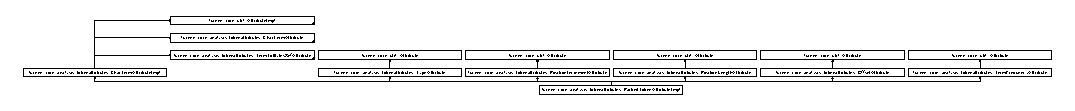
\includegraphics[height=1.049869cm]{classlucene_1_1core_1_1analysis_1_1tokenattributes_1_1PackedTokenAttributeImpl}
\end{center}
\end{figure}
\subsection*{Public Member Functions}
\begin{DoxyCompactItemize}
\item 
\mbox{\hyperlink{classlucene_1_1core_1_1analysis_1_1tokenattributes_1_1PackedTokenAttributeImpl_a11dff73c5a672c0fc89c2f69b5d6366d}{Packed\+Token\+Attribute\+Impl}} ()
\item 
\mbox{\hyperlink{classlucene_1_1core_1_1analysis_1_1tokenattributes_1_1PackedTokenAttributeImpl_a7f5ec442110c91b403513caa53691da4}{Packed\+Token\+Attribute\+Impl}} (\mbox{\hyperlink{ZlibCrc32_8h_a2c212835823e3c54a8ab6d95c652660e}{const}} \mbox{\hyperlink{classlucene_1_1core_1_1analysis_1_1tokenattributes_1_1PackedTokenAttributeImpl}{Packed\+Token\+Attribute\+Impl}} \&other)
\item 
virtual \mbox{\hyperlink{classlucene_1_1core_1_1analysis_1_1tokenattributes_1_1PackedTokenAttributeImpl_affb00f4d610f5827e13a8ede6ff081a7}{$\sim$\+Packed\+Token\+Attribute\+Impl}} ()
\item 
std\+::string \& \mbox{\hyperlink{classlucene_1_1core_1_1analysis_1_1tokenattributes_1_1PackedTokenAttributeImpl_ab9c0b48ded43a3c377136210dcbda215}{Type}} () override
\item 
void \mbox{\hyperlink{classlucene_1_1core_1_1analysis_1_1tokenattributes_1_1PackedTokenAttributeImpl_ad5f1b7e5437154dada3da8cc4f89c642}{Set\+Type}} (\mbox{\hyperlink{ZlibCrc32_8h_a2c212835823e3c54a8ab6d95c652660e}{const}} std\+::string \&new\+\_\+type) override
\item 
void \mbox{\hyperlink{classlucene_1_1core_1_1analysis_1_1tokenattributes_1_1PackedTokenAttributeImpl_a657933594f71883a7271bca05363bc2a}{Set\+Position\+Increment}} (\mbox{\hyperlink{ZlibCrc32_8h_a2c212835823e3c54a8ab6d95c652660e}{const}} uint32\+\_\+t new\+\_\+position\+\_\+increment) override
\item 
uint32\+\_\+t \mbox{\hyperlink{classlucene_1_1core_1_1analysis_1_1tokenattributes_1_1PackedTokenAttributeImpl_aeeb6d5e17fb510c402e36d50e39bb9fb}{Get\+Position\+Increment}} () override
\item 
void \mbox{\hyperlink{classlucene_1_1core_1_1analysis_1_1tokenattributes_1_1PackedTokenAttributeImpl_a3d721b90985cf600d2d44bb5f156d05d}{Set\+Position\+Length}} (\mbox{\hyperlink{ZlibCrc32_8h_a2c212835823e3c54a8ab6d95c652660e}{const}} uint32\+\_\+t new\+\_\+position\+\_\+length) override
\item 
uint32\+\_\+t \mbox{\hyperlink{classlucene_1_1core_1_1analysis_1_1tokenattributes_1_1PackedTokenAttributeImpl_a4b5a93a1d9b61cf1504b382d24c1e6d9}{Get\+Position\+Length}} () override
\item 
uint32\+\_\+t \mbox{\hyperlink{classlucene_1_1core_1_1analysis_1_1tokenattributes_1_1PackedTokenAttributeImpl_aea927563f771802e2ea6356814b53c17}{Start\+Offset}} () override
\item 
void \mbox{\hyperlink{classlucene_1_1core_1_1analysis_1_1tokenattributes_1_1PackedTokenAttributeImpl_aa17ed401f2b9f6bd773291de1d02bb35}{Set\+Offset}} (\mbox{\hyperlink{ZlibCrc32_8h_a2c212835823e3c54a8ab6d95c652660e}{const}} uint32\+\_\+t new\+\_\+start\+\_\+offset, \mbox{\hyperlink{ZlibCrc32_8h_a2c212835823e3c54a8ab6d95c652660e}{const}} uint32\+\_\+t new\+\_\+end\+\_\+offset) override
\item 
uint32\+\_\+t \mbox{\hyperlink{classlucene_1_1core_1_1analysis_1_1tokenattributes_1_1PackedTokenAttributeImpl_ae6210d544884be562c186a040d91157f}{End\+Offset}} () override
\item 
void \mbox{\hyperlink{classlucene_1_1core_1_1analysis_1_1tokenattributes_1_1PackedTokenAttributeImpl_a4d9dfc6cc7c825d42789245b8ca003c4}{Set\+Term\+Frequency}} (\mbox{\hyperlink{ZlibCrc32_8h_a2c212835823e3c54a8ab6d95c652660e}{const}} uint32\+\_\+t new\+\_\+term\+\_\+frequency) override
\item 
uint32\+\_\+t \mbox{\hyperlink{classlucene_1_1core_1_1analysis_1_1tokenattributes_1_1PackedTokenAttributeImpl_a82aff8ded68bf64ab156382ca6862db2}{Get\+Term\+Frequency}} () override
\item 
std\+::vector$<$ std\+::type\+\_\+index $>$ \mbox{\hyperlink{classlucene_1_1core_1_1analysis_1_1tokenattributes_1_1PackedTokenAttributeImpl_a450b5fd90cbf05268800b0f66eebb58f}{Attributes}} () override
\item 
void \mbox{\hyperlink{classlucene_1_1core_1_1analysis_1_1tokenattributes_1_1PackedTokenAttributeImpl_ab89c820321f0f5b84c7a392bb8de32f3}{Shallow\+Copy\+To}} (\mbox{\hyperlink{classlucene_1_1core_1_1util_1_1AttributeImpl}{lucene\+::core\+::util\+::\+Attribute\+Impl}} \&attr\+\_\+impl) override
\item 
\mbox{\hyperlink{classlucene_1_1core_1_1analysis_1_1tokenattributes_1_1PackedTokenAttributeImpl}{Packed\+Token\+Attribute\+Impl}} \& \mbox{\hyperlink{classlucene_1_1core_1_1analysis_1_1tokenattributes_1_1PackedTokenAttributeImpl_a9519720f5eb790ef3e796cefbcbecc96}{operator=}} (\mbox{\hyperlink{ZlibCrc32_8h_a2c212835823e3c54a8ab6d95c652660e}{const}} \mbox{\hyperlink{classlucene_1_1core_1_1util_1_1AttributeImpl}{lucene\+::core\+::util\+::\+Attribute\+Impl}} \&other)
\item 
\mbox{\hyperlink{classlucene_1_1core_1_1analysis_1_1tokenattributes_1_1PackedTokenAttributeImpl}{Packed\+Token\+Attribute\+Impl}} \& \mbox{\hyperlink{classlucene_1_1core_1_1analysis_1_1tokenattributes_1_1PackedTokenAttributeImpl_a87fbfcbb26c03dc5fd6d6d51fc41e817}{operator=}} (\mbox{\hyperlink{ZlibCrc32_8h_a2c212835823e3c54a8ab6d95c652660e}{const}} \mbox{\hyperlink{classlucene_1_1core_1_1analysis_1_1tokenattributes_1_1PackedTokenAttributeImpl}{Packed\+Token\+Attribute\+Impl}} \&other)
\item 
\mbox{\hyperlink{classlucene_1_1core_1_1util_1_1AttributeImpl}{lucene\+::core\+::util\+::\+Attribute\+Impl}} $\ast$ \mbox{\hyperlink{classlucene_1_1core_1_1analysis_1_1tokenattributes_1_1PackedTokenAttributeImpl_ab96495b9ba0271afe2597425f925ee91}{Clone}} () override
\end{DoxyCompactItemize}
\subsection*{Private Attributes}
\begin{DoxyCompactItemize}
\item 
uint32\+\_\+t \mbox{\hyperlink{classlucene_1_1core_1_1analysis_1_1tokenattributes_1_1PackedTokenAttributeImpl_a15d9f4ff5be2008f86e853cabff85566}{start\+\_\+offset}}
\item 
uint32\+\_\+t \mbox{\hyperlink{classlucene_1_1core_1_1analysis_1_1tokenattributes_1_1PackedTokenAttributeImpl_ae3b9bf799d0a6645eafbda1b01094e81}{end\+\_\+offset}}
\item 
std\+::string \mbox{\hyperlink{classlucene_1_1core_1_1analysis_1_1tokenattributes_1_1PackedTokenAttributeImpl_a39f37a016d846f19589fda8383489164}{type}}
\item 
uint32\+\_\+t \mbox{\hyperlink{classlucene_1_1core_1_1analysis_1_1tokenattributes_1_1PackedTokenAttributeImpl_ab999325a1f0d535a767f924fcd3954c5}{position\+\_\+increment}}
\item 
uint32\+\_\+t \mbox{\hyperlink{classlucene_1_1core_1_1analysis_1_1tokenattributes_1_1PackedTokenAttributeImpl_aaed2579a261b29b608ed68aa2b7728fd}{position\+\_\+length}}
\item 
uint32\+\_\+t \mbox{\hyperlink{classlucene_1_1core_1_1analysis_1_1tokenattributes_1_1PackedTokenAttributeImpl_a415328f42ee5fc7e0a39479b7e3a8f67}{term\+\_\+frequency}}
\end{DoxyCompactItemize}
\subsection*{Additional Inherited Members}


\subsection{Constructor \& Destructor Documentation}
\mbox{\Hypertarget{classlucene_1_1core_1_1analysis_1_1tokenattributes_1_1PackedTokenAttributeImpl_a11dff73c5a672c0fc89c2f69b5d6366d}\label{classlucene_1_1core_1_1analysis_1_1tokenattributes_1_1PackedTokenAttributeImpl_a11dff73c5a672c0fc89c2f69b5d6366d}} 
\index{lucene\+::core\+::analysis\+::tokenattributes\+::\+Packed\+Token\+Attribute\+Impl@{lucene\+::core\+::analysis\+::tokenattributes\+::\+Packed\+Token\+Attribute\+Impl}!Packed\+Token\+Attribute\+Impl@{Packed\+Token\+Attribute\+Impl}}
\index{Packed\+Token\+Attribute\+Impl@{Packed\+Token\+Attribute\+Impl}!lucene\+::core\+::analysis\+::tokenattributes\+::\+Packed\+Token\+Attribute\+Impl@{lucene\+::core\+::analysis\+::tokenattributes\+::\+Packed\+Token\+Attribute\+Impl}}
\subsubsection{\texorpdfstring{Packed\+Token\+Attribute\+Impl()}{PackedTokenAttributeImpl()}\hspace{0.1cm}{\footnotesize\ttfamily [1/2]}}
{\footnotesize\ttfamily Packed\+Token\+Attribute\+Impl\+::\+Packed\+Token\+Attribute\+Impl (\begin{DoxyParamCaption}{ }\end{DoxyParamCaption})}

\mbox{\hyperlink{classlucene_1_1core_1_1analysis_1_1tokenattributes_1_1PackedTokenAttributeImpl}{Packed\+Token\+Attribute\+Impl}} \mbox{\Hypertarget{classlucene_1_1core_1_1analysis_1_1tokenattributes_1_1PackedTokenAttributeImpl_a7f5ec442110c91b403513caa53691da4}\label{classlucene_1_1core_1_1analysis_1_1tokenattributes_1_1PackedTokenAttributeImpl_a7f5ec442110c91b403513caa53691da4}} 
\index{lucene\+::core\+::analysis\+::tokenattributes\+::\+Packed\+Token\+Attribute\+Impl@{lucene\+::core\+::analysis\+::tokenattributes\+::\+Packed\+Token\+Attribute\+Impl}!Packed\+Token\+Attribute\+Impl@{Packed\+Token\+Attribute\+Impl}}
\index{Packed\+Token\+Attribute\+Impl@{Packed\+Token\+Attribute\+Impl}!lucene\+::core\+::analysis\+::tokenattributes\+::\+Packed\+Token\+Attribute\+Impl@{lucene\+::core\+::analysis\+::tokenattributes\+::\+Packed\+Token\+Attribute\+Impl}}
\subsubsection{\texorpdfstring{Packed\+Token\+Attribute\+Impl()}{PackedTokenAttributeImpl()}\hspace{0.1cm}{\footnotesize\ttfamily [2/2]}}
{\footnotesize\ttfamily Packed\+Token\+Attribute\+Impl\+::\+Packed\+Token\+Attribute\+Impl (\begin{DoxyParamCaption}\item[{\mbox{\hyperlink{ZlibCrc32_8h_a2c212835823e3c54a8ab6d95c652660e}{const}} \mbox{\hyperlink{classlucene_1_1core_1_1analysis_1_1tokenattributes_1_1PackedTokenAttributeImpl}{Packed\+Token\+Attribute\+Impl}} \&}]{other }\end{DoxyParamCaption})}

\mbox{\Hypertarget{classlucene_1_1core_1_1analysis_1_1tokenattributes_1_1PackedTokenAttributeImpl_affb00f4d610f5827e13a8ede6ff081a7}\label{classlucene_1_1core_1_1analysis_1_1tokenattributes_1_1PackedTokenAttributeImpl_affb00f4d610f5827e13a8ede6ff081a7}} 
\index{lucene\+::core\+::analysis\+::tokenattributes\+::\+Packed\+Token\+Attribute\+Impl@{lucene\+::core\+::analysis\+::tokenattributes\+::\+Packed\+Token\+Attribute\+Impl}!````~Packed\+Token\+Attribute\+Impl@{$\sim$\+Packed\+Token\+Attribute\+Impl}}
\index{````~Packed\+Token\+Attribute\+Impl@{$\sim$\+Packed\+Token\+Attribute\+Impl}!lucene\+::core\+::analysis\+::tokenattributes\+::\+Packed\+Token\+Attribute\+Impl@{lucene\+::core\+::analysis\+::tokenattributes\+::\+Packed\+Token\+Attribute\+Impl}}
\subsubsection{\texorpdfstring{$\sim$\+Packed\+Token\+Attribute\+Impl()}{~PackedTokenAttributeImpl()}}
{\footnotesize\ttfamily Packed\+Token\+Attribute\+Impl\+::$\sim$\+Packed\+Token\+Attribute\+Impl (\begin{DoxyParamCaption}{ }\end{DoxyParamCaption})\hspace{0.3cm}{\ttfamily [virtual]}}



\subsection{Member Function Documentation}
\mbox{\Hypertarget{classlucene_1_1core_1_1analysis_1_1tokenattributes_1_1PackedTokenAttributeImpl_a450b5fd90cbf05268800b0f66eebb58f}\label{classlucene_1_1core_1_1analysis_1_1tokenattributes_1_1PackedTokenAttributeImpl_a450b5fd90cbf05268800b0f66eebb58f}} 
\index{lucene\+::core\+::analysis\+::tokenattributes\+::\+Packed\+Token\+Attribute\+Impl@{lucene\+::core\+::analysis\+::tokenattributes\+::\+Packed\+Token\+Attribute\+Impl}!Attributes@{Attributes}}
\index{Attributes@{Attributes}!lucene\+::core\+::analysis\+::tokenattributes\+::\+Packed\+Token\+Attribute\+Impl@{lucene\+::core\+::analysis\+::tokenattributes\+::\+Packed\+Token\+Attribute\+Impl}}
\subsubsection{\texorpdfstring{Attributes()}{Attributes()}}
{\footnotesize\ttfamily std\+::vector$<$ std\+::type\+\_\+index $>$ Packed\+Token\+Attribute\+Impl\+::\+Attributes (\begin{DoxyParamCaption}{ }\end{DoxyParamCaption})\hspace{0.3cm}{\ttfamily [override]}, {\ttfamily [virtual]}}



Reimplemented from \mbox{\hyperlink{classlucene_1_1core_1_1analysis_1_1tokenattributes_1_1CharTermAttributeImpl_a7d8986b373cd9c2dfb2de25dd12000fd}{lucene\+::core\+::analysis\+::tokenattributes\+::\+Char\+Term\+Attribute\+Impl}}.

\mbox{\Hypertarget{classlucene_1_1core_1_1analysis_1_1tokenattributes_1_1PackedTokenAttributeImpl_ab96495b9ba0271afe2597425f925ee91}\label{classlucene_1_1core_1_1analysis_1_1tokenattributes_1_1PackedTokenAttributeImpl_ab96495b9ba0271afe2597425f925ee91}} 
\index{lucene\+::core\+::analysis\+::tokenattributes\+::\+Packed\+Token\+Attribute\+Impl@{lucene\+::core\+::analysis\+::tokenattributes\+::\+Packed\+Token\+Attribute\+Impl}!Clone@{Clone}}
\index{Clone@{Clone}!lucene\+::core\+::analysis\+::tokenattributes\+::\+Packed\+Token\+Attribute\+Impl@{lucene\+::core\+::analysis\+::tokenattributes\+::\+Packed\+Token\+Attribute\+Impl}}
\subsubsection{\texorpdfstring{Clone()}{Clone()}}
{\footnotesize\ttfamily \mbox{\hyperlink{classlucene_1_1core_1_1util_1_1AttributeImpl}{Attribute\+Impl}} $\ast$ Packed\+Token\+Attribute\+Impl\+::\+Clone (\begin{DoxyParamCaption}{ }\end{DoxyParamCaption})\hspace{0.3cm}{\ttfamily [override]}, {\ttfamily [virtual]}}



Reimplemented from \mbox{\hyperlink{classlucene_1_1core_1_1analysis_1_1tokenattributes_1_1CharTermAttributeImpl_a518bf3f405ddf676ee58fccb02ae3c23}{lucene\+::core\+::analysis\+::tokenattributes\+::\+Char\+Term\+Attribute\+Impl}}.

\mbox{\Hypertarget{classlucene_1_1core_1_1analysis_1_1tokenattributes_1_1PackedTokenAttributeImpl_ae6210d544884be562c186a040d91157f}\label{classlucene_1_1core_1_1analysis_1_1tokenattributes_1_1PackedTokenAttributeImpl_ae6210d544884be562c186a040d91157f}} 
\index{lucene\+::core\+::analysis\+::tokenattributes\+::\+Packed\+Token\+Attribute\+Impl@{lucene\+::core\+::analysis\+::tokenattributes\+::\+Packed\+Token\+Attribute\+Impl}!End\+Offset@{End\+Offset}}
\index{End\+Offset@{End\+Offset}!lucene\+::core\+::analysis\+::tokenattributes\+::\+Packed\+Token\+Attribute\+Impl@{lucene\+::core\+::analysis\+::tokenattributes\+::\+Packed\+Token\+Attribute\+Impl}}
\subsubsection{\texorpdfstring{End\+Offset()}{EndOffset()}}
{\footnotesize\ttfamily uint32\+\_\+t Packed\+Token\+Attribute\+Impl\+::\+End\+Offset (\begin{DoxyParamCaption}{ }\end{DoxyParamCaption})\hspace{0.3cm}{\ttfamily [override]}, {\ttfamily [virtual]}}



Implements \mbox{\hyperlink{classlucene_1_1core_1_1analysis_1_1tokenattributes_1_1OffsetAttribute_ada281ff6240e1a0fecf57707329ec974}{lucene\+::core\+::analysis\+::tokenattributes\+::\+Offset\+Attribute}}.

\mbox{\Hypertarget{classlucene_1_1core_1_1analysis_1_1tokenattributes_1_1PackedTokenAttributeImpl_aeeb6d5e17fb510c402e36d50e39bb9fb}\label{classlucene_1_1core_1_1analysis_1_1tokenattributes_1_1PackedTokenAttributeImpl_aeeb6d5e17fb510c402e36d50e39bb9fb}} 
\index{lucene\+::core\+::analysis\+::tokenattributes\+::\+Packed\+Token\+Attribute\+Impl@{lucene\+::core\+::analysis\+::tokenattributes\+::\+Packed\+Token\+Attribute\+Impl}!Get\+Position\+Increment@{Get\+Position\+Increment}}
\index{Get\+Position\+Increment@{Get\+Position\+Increment}!lucene\+::core\+::analysis\+::tokenattributes\+::\+Packed\+Token\+Attribute\+Impl@{lucene\+::core\+::analysis\+::tokenattributes\+::\+Packed\+Token\+Attribute\+Impl}}
\subsubsection{\texorpdfstring{Get\+Position\+Increment()}{GetPositionIncrement()}}
{\footnotesize\ttfamily uint32\+\_\+t Packed\+Token\+Attribute\+Impl\+::\+Get\+Position\+Increment (\begin{DoxyParamCaption}{ }\end{DoxyParamCaption})\hspace{0.3cm}{\ttfamily [override]}, {\ttfamily [virtual]}}



Implements \mbox{\hyperlink{classlucene_1_1core_1_1analysis_1_1tokenattributes_1_1PositionIncrementAttribute_af0c59c3fbf138881647e46f05468eb13}{lucene\+::core\+::analysis\+::tokenattributes\+::\+Position\+Increment\+Attribute}}.

\mbox{\Hypertarget{classlucene_1_1core_1_1analysis_1_1tokenattributes_1_1PackedTokenAttributeImpl_a4b5a93a1d9b61cf1504b382d24c1e6d9}\label{classlucene_1_1core_1_1analysis_1_1tokenattributes_1_1PackedTokenAttributeImpl_a4b5a93a1d9b61cf1504b382d24c1e6d9}} 
\index{lucene\+::core\+::analysis\+::tokenattributes\+::\+Packed\+Token\+Attribute\+Impl@{lucene\+::core\+::analysis\+::tokenattributes\+::\+Packed\+Token\+Attribute\+Impl}!Get\+Position\+Length@{Get\+Position\+Length}}
\index{Get\+Position\+Length@{Get\+Position\+Length}!lucene\+::core\+::analysis\+::tokenattributes\+::\+Packed\+Token\+Attribute\+Impl@{lucene\+::core\+::analysis\+::tokenattributes\+::\+Packed\+Token\+Attribute\+Impl}}
\subsubsection{\texorpdfstring{Get\+Position\+Length()}{GetPositionLength()}}
{\footnotesize\ttfamily uint32\+\_\+t Packed\+Token\+Attribute\+Impl\+::\+Get\+Position\+Length (\begin{DoxyParamCaption}{ }\end{DoxyParamCaption})\hspace{0.3cm}{\ttfamily [override]}, {\ttfamily [virtual]}}



Implements \mbox{\hyperlink{classlucene_1_1core_1_1analysis_1_1tokenattributes_1_1PositionLengthAttribute_a6325424899959bb480f161e0d5490bfd}{lucene\+::core\+::analysis\+::tokenattributes\+::\+Position\+Length\+Attribute}}.

\mbox{\Hypertarget{classlucene_1_1core_1_1analysis_1_1tokenattributes_1_1PackedTokenAttributeImpl_a82aff8ded68bf64ab156382ca6862db2}\label{classlucene_1_1core_1_1analysis_1_1tokenattributes_1_1PackedTokenAttributeImpl_a82aff8ded68bf64ab156382ca6862db2}} 
\index{lucene\+::core\+::analysis\+::tokenattributes\+::\+Packed\+Token\+Attribute\+Impl@{lucene\+::core\+::analysis\+::tokenattributes\+::\+Packed\+Token\+Attribute\+Impl}!Get\+Term\+Frequency@{Get\+Term\+Frequency}}
\index{Get\+Term\+Frequency@{Get\+Term\+Frequency}!lucene\+::core\+::analysis\+::tokenattributes\+::\+Packed\+Token\+Attribute\+Impl@{lucene\+::core\+::analysis\+::tokenattributes\+::\+Packed\+Token\+Attribute\+Impl}}
\subsubsection{\texorpdfstring{Get\+Term\+Frequency()}{GetTermFrequency()}}
{\footnotesize\ttfamily uint32\+\_\+t Packed\+Token\+Attribute\+Impl\+::\+Get\+Term\+Frequency (\begin{DoxyParamCaption}{ }\end{DoxyParamCaption})\hspace{0.3cm}{\ttfamily [override]}, {\ttfamily [virtual]}}



Implements \mbox{\hyperlink{classlucene_1_1core_1_1analysis_1_1tokenattributes_1_1TermFrequencyAttribute_a2ddffa369215ac61e2eadbab087f5d74}{lucene\+::core\+::analysis\+::tokenattributes\+::\+Term\+Frequency\+Attribute}}.

\mbox{\Hypertarget{classlucene_1_1core_1_1analysis_1_1tokenattributes_1_1PackedTokenAttributeImpl_a9519720f5eb790ef3e796cefbcbecc96}\label{classlucene_1_1core_1_1analysis_1_1tokenattributes_1_1PackedTokenAttributeImpl_a9519720f5eb790ef3e796cefbcbecc96}} 
\index{lucene\+::core\+::analysis\+::tokenattributes\+::\+Packed\+Token\+Attribute\+Impl@{lucene\+::core\+::analysis\+::tokenattributes\+::\+Packed\+Token\+Attribute\+Impl}!operator=@{operator=}}
\index{operator=@{operator=}!lucene\+::core\+::analysis\+::tokenattributes\+::\+Packed\+Token\+Attribute\+Impl@{lucene\+::core\+::analysis\+::tokenattributes\+::\+Packed\+Token\+Attribute\+Impl}}
\subsubsection{\texorpdfstring{operator=()}{operator=()}\hspace{0.1cm}{\footnotesize\ttfamily [1/2]}}
{\footnotesize\ttfamily \mbox{\hyperlink{classlucene_1_1core_1_1analysis_1_1tokenattributes_1_1PackedTokenAttributeImpl}{Packed\+Token\+Attribute\+Impl}} \& Packed\+Token\+Attribute\+Impl\+::operator= (\begin{DoxyParamCaption}\item[{\mbox{\hyperlink{ZlibCrc32_8h_a2c212835823e3c54a8ab6d95c652660e}{const}} \mbox{\hyperlink{classlucene_1_1core_1_1util_1_1AttributeImpl}{lucene\+::core\+::util\+::\+Attribute\+Impl}} \&}]{other }\end{DoxyParamCaption})\hspace{0.3cm}{\ttfamily [virtual]}}



Reimplemented from \mbox{\hyperlink{classlucene_1_1core_1_1analysis_1_1tokenattributes_1_1CharTermAttributeImpl_ac49b714c3f8e438ddaa27dc1a2421144}{lucene\+::core\+::analysis\+::tokenattributes\+::\+Char\+Term\+Attribute\+Impl}}.

\mbox{\Hypertarget{classlucene_1_1core_1_1analysis_1_1tokenattributes_1_1PackedTokenAttributeImpl_a87fbfcbb26c03dc5fd6d6d51fc41e817}\label{classlucene_1_1core_1_1analysis_1_1tokenattributes_1_1PackedTokenAttributeImpl_a87fbfcbb26c03dc5fd6d6d51fc41e817}} 
\index{lucene\+::core\+::analysis\+::tokenattributes\+::\+Packed\+Token\+Attribute\+Impl@{lucene\+::core\+::analysis\+::tokenattributes\+::\+Packed\+Token\+Attribute\+Impl}!operator=@{operator=}}
\index{operator=@{operator=}!lucene\+::core\+::analysis\+::tokenattributes\+::\+Packed\+Token\+Attribute\+Impl@{lucene\+::core\+::analysis\+::tokenattributes\+::\+Packed\+Token\+Attribute\+Impl}}
\subsubsection{\texorpdfstring{operator=()}{operator=()}\hspace{0.1cm}{\footnotesize\ttfamily [2/2]}}
{\footnotesize\ttfamily \mbox{\hyperlink{classlucene_1_1core_1_1analysis_1_1tokenattributes_1_1PackedTokenAttributeImpl}{Packed\+Token\+Attribute\+Impl}} \& Packed\+Token\+Attribute\+Impl\+::operator= (\begin{DoxyParamCaption}\item[{\mbox{\hyperlink{ZlibCrc32_8h_a2c212835823e3c54a8ab6d95c652660e}{const}} \mbox{\hyperlink{classlucene_1_1core_1_1analysis_1_1tokenattributes_1_1PackedTokenAttributeImpl}{Packed\+Token\+Attribute\+Impl}} \&}]{other }\end{DoxyParamCaption})}

\mbox{\Hypertarget{classlucene_1_1core_1_1analysis_1_1tokenattributes_1_1PackedTokenAttributeImpl_aa17ed401f2b9f6bd773291de1d02bb35}\label{classlucene_1_1core_1_1analysis_1_1tokenattributes_1_1PackedTokenAttributeImpl_aa17ed401f2b9f6bd773291de1d02bb35}} 
\index{lucene\+::core\+::analysis\+::tokenattributes\+::\+Packed\+Token\+Attribute\+Impl@{lucene\+::core\+::analysis\+::tokenattributes\+::\+Packed\+Token\+Attribute\+Impl}!Set\+Offset@{Set\+Offset}}
\index{Set\+Offset@{Set\+Offset}!lucene\+::core\+::analysis\+::tokenattributes\+::\+Packed\+Token\+Attribute\+Impl@{lucene\+::core\+::analysis\+::tokenattributes\+::\+Packed\+Token\+Attribute\+Impl}}
\subsubsection{\texorpdfstring{Set\+Offset()}{SetOffset()}}
{\footnotesize\ttfamily void Packed\+Token\+Attribute\+Impl\+::\+Set\+Offset (\begin{DoxyParamCaption}\item[{\mbox{\hyperlink{ZlibCrc32_8h_a2c212835823e3c54a8ab6d95c652660e}{const}} uint32\+\_\+t}]{new\+\_\+start\+\_\+offset,  }\item[{\mbox{\hyperlink{ZlibCrc32_8h_a2c212835823e3c54a8ab6d95c652660e}{const}} uint32\+\_\+t}]{new\+\_\+end\+\_\+offset }\end{DoxyParamCaption})\hspace{0.3cm}{\ttfamily [override]}, {\ttfamily [virtual]}}



Implements \mbox{\hyperlink{classlucene_1_1core_1_1analysis_1_1tokenattributes_1_1OffsetAttribute_aa0d076ac2e7c5af86668fbbeb8e26170}{lucene\+::core\+::analysis\+::tokenattributes\+::\+Offset\+Attribute}}.

\mbox{\Hypertarget{classlucene_1_1core_1_1analysis_1_1tokenattributes_1_1PackedTokenAttributeImpl_a657933594f71883a7271bca05363bc2a}\label{classlucene_1_1core_1_1analysis_1_1tokenattributes_1_1PackedTokenAttributeImpl_a657933594f71883a7271bca05363bc2a}} 
\index{lucene\+::core\+::analysis\+::tokenattributes\+::\+Packed\+Token\+Attribute\+Impl@{lucene\+::core\+::analysis\+::tokenattributes\+::\+Packed\+Token\+Attribute\+Impl}!Set\+Position\+Increment@{Set\+Position\+Increment}}
\index{Set\+Position\+Increment@{Set\+Position\+Increment}!lucene\+::core\+::analysis\+::tokenattributes\+::\+Packed\+Token\+Attribute\+Impl@{lucene\+::core\+::analysis\+::tokenattributes\+::\+Packed\+Token\+Attribute\+Impl}}
\subsubsection{\texorpdfstring{Set\+Position\+Increment()}{SetPositionIncrement()}}
{\footnotesize\ttfamily void Packed\+Token\+Attribute\+Impl\+::\+Set\+Position\+Increment (\begin{DoxyParamCaption}\item[{\mbox{\hyperlink{ZlibCrc32_8h_a2c212835823e3c54a8ab6d95c652660e}{const}} uint32\+\_\+t}]{new\+\_\+position\+\_\+increment }\end{DoxyParamCaption})\hspace{0.3cm}{\ttfamily [override]}, {\ttfamily [virtual]}}



Implements \mbox{\hyperlink{classlucene_1_1core_1_1analysis_1_1tokenattributes_1_1PositionIncrementAttribute_a7d012852b01e0b16da72a911a90266b7}{lucene\+::core\+::analysis\+::tokenattributes\+::\+Position\+Increment\+Attribute}}.

\mbox{\Hypertarget{classlucene_1_1core_1_1analysis_1_1tokenattributes_1_1PackedTokenAttributeImpl_a3d721b90985cf600d2d44bb5f156d05d}\label{classlucene_1_1core_1_1analysis_1_1tokenattributes_1_1PackedTokenAttributeImpl_a3d721b90985cf600d2d44bb5f156d05d}} 
\index{lucene\+::core\+::analysis\+::tokenattributes\+::\+Packed\+Token\+Attribute\+Impl@{lucene\+::core\+::analysis\+::tokenattributes\+::\+Packed\+Token\+Attribute\+Impl}!Set\+Position\+Length@{Set\+Position\+Length}}
\index{Set\+Position\+Length@{Set\+Position\+Length}!lucene\+::core\+::analysis\+::tokenattributes\+::\+Packed\+Token\+Attribute\+Impl@{lucene\+::core\+::analysis\+::tokenattributes\+::\+Packed\+Token\+Attribute\+Impl}}
\subsubsection{\texorpdfstring{Set\+Position\+Length()}{SetPositionLength()}}
{\footnotesize\ttfamily void Packed\+Token\+Attribute\+Impl\+::\+Set\+Position\+Length (\begin{DoxyParamCaption}\item[{\mbox{\hyperlink{ZlibCrc32_8h_a2c212835823e3c54a8ab6d95c652660e}{const}} uint32\+\_\+t}]{new\+\_\+position\+\_\+length }\end{DoxyParamCaption})\hspace{0.3cm}{\ttfamily [override]}, {\ttfamily [virtual]}}



Implements \mbox{\hyperlink{classlucene_1_1core_1_1analysis_1_1tokenattributes_1_1PositionLengthAttribute_a514415965bae0dd392cbb8d65ea4d808}{lucene\+::core\+::analysis\+::tokenattributes\+::\+Position\+Length\+Attribute}}.

\mbox{\Hypertarget{classlucene_1_1core_1_1analysis_1_1tokenattributes_1_1PackedTokenAttributeImpl_a4d9dfc6cc7c825d42789245b8ca003c4}\label{classlucene_1_1core_1_1analysis_1_1tokenattributes_1_1PackedTokenAttributeImpl_a4d9dfc6cc7c825d42789245b8ca003c4}} 
\index{lucene\+::core\+::analysis\+::tokenattributes\+::\+Packed\+Token\+Attribute\+Impl@{lucene\+::core\+::analysis\+::tokenattributes\+::\+Packed\+Token\+Attribute\+Impl}!Set\+Term\+Frequency@{Set\+Term\+Frequency}}
\index{Set\+Term\+Frequency@{Set\+Term\+Frequency}!lucene\+::core\+::analysis\+::tokenattributes\+::\+Packed\+Token\+Attribute\+Impl@{lucene\+::core\+::analysis\+::tokenattributes\+::\+Packed\+Token\+Attribute\+Impl}}
\subsubsection{\texorpdfstring{Set\+Term\+Frequency()}{SetTermFrequency()}}
{\footnotesize\ttfamily void Packed\+Token\+Attribute\+Impl\+::\+Set\+Term\+Frequency (\begin{DoxyParamCaption}\item[{\mbox{\hyperlink{ZlibCrc32_8h_a2c212835823e3c54a8ab6d95c652660e}{const}} uint32\+\_\+t}]{new\+\_\+term\+\_\+frequency }\end{DoxyParamCaption})\hspace{0.3cm}{\ttfamily [override]}, {\ttfamily [virtual]}}



Implements \mbox{\hyperlink{classlucene_1_1core_1_1analysis_1_1tokenattributes_1_1TermFrequencyAttribute_aeb8ef8cc3f3ab6c8678b491ac3e1b682}{lucene\+::core\+::analysis\+::tokenattributes\+::\+Term\+Frequency\+Attribute}}.

\mbox{\Hypertarget{classlucene_1_1core_1_1analysis_1_1tokenattributes_1_1PackedTokenAttributeImpl_ad5f1b7e5437154dada3da8cc4f89c642}\label{classlucene_1_1core_1_1analysis_1_1tokenattributes_1_1PackedTokenAttributeImpl_ad5f1b7e5437154dada3da8cc4f89c642}} 
\index{lucene\+::core\+::analysis\+::tokenattributes\+::\+Packed\+Token\+Attribute\+Impl@{lucene\+::core\+::analysis\+::tokenattributes\+::\+Packed\+Token\+Attribute\+Impl}!Set\+Type@{Set\+Type}}
\index{Set\+Type@{Set\+Type}!lucene\+::core\+::analysis\+::tokenattributes\+::\+Packed\+Token\+Attribute\+Impl@{lucene\+::core\+::analysis\+::tokenattributes\+::\+Packed\+Token\+Attribute\+Impl}}
\subsubsection{\texorpdfstring{Set\+Type()}{SetType()}}
{\footnotesize\ttfamily void Packed\+Token\+Attribute\+Impl\+::\+Set\+Type (\begin{DoxyParamCaption}\item[{\mbox{\hyperlink{ZlibCrc32_8h_a2c212835823e3c54a8ab6d95c652660e}{const}} std\+::string \&}]{new\+\_\+type }\end{DoxyParamCaption})\hspace{0.3cm}{\ttfamily [override]}, {\ttfamily [virtual]}}



Implements \mbox{\hyperlink{classlucene_1_1core_1_1analysis_1_1tokenattributes_1_1TypeAttribute_abb4ecef2fd30c7b659efd7f3a2086945}{lucene\+::core\+::analysis\+::tokenattributes\+::\+Type\+Attribute}}.

\mbox{\Hypertarget{classlucene_1_1core_1_1analysis_1_1tokenattributes_1_1PackedTokenAttributeImpl_ab89c820321f0f5b84c7a392bb8de32f3}\label{classlucene_1_1core_1_1analysis_1_1tokenattributes_1_1PackedTokenAttributeImpl_ab89c820321f0f5b84c7a392bb8de32f3}} 
\index{lucene\+::core\+::analysis\+::tokenattributes\+::\+Packed\+Token\+Attribute\+Impl@{lucene\+::core\+::analysis\+::tokenattributes\+::\+Packed\+Token\+Attribute\+Impl}!Shallow\+Copy\+To@{Shallow\+Copy\+To}}
\index{Shallow\+Copy\+To@{Shallow\+Copy\+To}!lucene\+::core\+::analysis\+::tokenattributes\+::\+Packed\+Token\+Attribute\+Impl@{lucene\+::core\+::analysis\+::tokenattributes\+::\+Packed\+Token\+Attribute\+Impl}}
\subsubsection{\texorpdfstring{Shallow\+Copy\+To()}{ShallowCopyTo()}}
{\footnotesize\ttfamily void Packed\+Token\+Attribute\+Impl\+::\+Shallow\+Copy\+To (\begin{DoxyParamCaption}\item[{\mbox{\hyperlink{classlucene_1_1core_1_1util_1_1AttributeImpl}{lucene\+::core\+::util\+::\+Attribute\+Impl}} \&}]{attr\+\_\+impl }\end{DoxyParamCaption})\hspace{0.3cm}{\ttfamily [override]}, {\ttfamily [virtual]}}



Reimplemented from \mbox{\hyperlink{classlucene_1_1core_1_1analysis_1_1tokenattributes_1_1CharTermAttributeImpl_ae37cc1fbce5614f5e60800d3f9f96d33}{lucene\+::core\+::analysis\+::tokenattributes\+::\+Char\+Term\+Attribute\+Impl}}.

\mbox{\Hypertarget{classlucene_1_1core_1_1analysis_1_1tokenattributes_1_1PackedTokenAttributeImpl_aea927563f771802e2ea6356814b53c17}\label{classlucene_1_1core_1_1analysis_1_1tokenattributes_1_1PackedTokenAttributeImpl_aea927563f771802e2ea6356814b53c17}} 
\index{lucene\+::core\+::analysis\+::tokenattributes\+::\+Packed\+Token\+Attribute\+Impl@{lucene\+::core\+::analysis\+::tokenattributes\+::\+Packed\+Token\+Attribute\+Impl}!Start\+Offset@{Start\+Offset}}
\index{Start\+Offset@{Start\+Offset}!lucene\+::core\+::analysis\+::tokenattributes\+::\+Packed\+Token\+Attribute\+Impl@{lucene\+::core\+::analysis\+::tokenattributes\+::\+Packed\+Token\+Attribute\+Impl}}
\subsubsection{\texorpdfstring{Start\+Offset()}{StartOffset()}}
{\footnotesize\ttfamily uint32\+\_\+t Packed\+Token\+Attribute\+Impl\+::\+Start\+Offset (\begin{DoxyParamCaption}{ }\end{DoxyParamCaption})\hspace{0.3cm}{\ttfamily [override]}, {\ttfamily [virtual]}}



Implements \mbox{\hyperlink{classlucene_1_1core_1_1analysis_1_1tokenattributes_1_1OffsetAttribute_af841d190a7900a5b6a00f0a9f4ae7e43}{lucene\+::core\+::analysis\+::tokenattributes\+::\+Offset\+Attribute}}.

\mbox{\Hypertarget{classlucene_1_1core_1_1analysis_1_1tokenattributes_1_1PackedTokenAttributeImpl_ab9c0b48ded43a3c377136210dcbda215}\label{classlucene_1_1core_1_1analysis_1_1tokenattributes_1_1PackedTokenAttributeImpl_ab9c0b48ded43a3c377136210dcbda215}} 
\index{lucene\+::core\+::analysis\+::tokenattributes\+::\+Packed\+Token\+Attribute\+Impl@{lucene\+::core\+::analysis\+::tokenattributes\+::\+Packed\+Token\+Attribute\+Impl}!Type@{Type}}
\index{Type@{Type}!lucene\+::core\+::analysis\+::tokenattributes\+::\+Packed\+Token\+Attribute\+Impl@{lucene\+::core\+::analysis\+::tokenattributes\+::\+Packed\+Token\+Attribute\+Impl}}
\subsubsection{\texorpdfstring{Type()}{Type()}}
{\footnotesize\ttfamily std\+::string \& Packed\+Token\+Attribute\+Impl\+::\+Type (\begin{DoxyParamCaption}{ }\end{DoxyParamCaption})\hspace{0.3cm}{\ttfamily [override]}, {\ttfamily [virtual]}}



Implements \mbox{\hyperlink{classlucene_1_1core_1_1analysis_1_1tokenattributes_1_1TypeAttribute_a85bef723dc92f76228982ff3907c5d04}{lucene\+::core\+::analysis\+::tokenattributes\+::\+Type\+Attribute}}.



\subsection{Member Data Documentation}
\mbox{\Hypertarget{classlucene_1_1core_1_1analysis_1_1tokenattributes_1_1PackedTokenAttributeImpl_ae3b9bf799d0a6645eafbda1b01094e81}\label{classlucene_1_1core_1_1analysis_1_1tokenattributes_1_1PackedTokenAttributeImpl_ae3b9bf799d0a6645eafbda1b01094e81}} 
\index{lucene\+::core\+::analysis\+::tokenattributes\+::\+Packed\+Token\+Attribute\+Impl@{lucene\+::core\+::analysis\+::tokenattributes\+::\+Packed\+Token\+Attribute\+Impl}!end\+\_\+offset@{end\+\_\+offset}}
\index{end\+\_\+offset@{end\+\_\+offset}!lucene\+::core\+::analysis\+::tokenattributes\+::\+Packed\+Token\+Attribute\+Impl@{lucene\+::core\+::analysis\+::tokenattributes\+::\+Packed\+Token\+Attribute\+Impl}}
\subsubsection{\texorpdfstring{end\+\_\+offset}{end\_offset}}
{\footnotesize\ttfamily uint32\+\_\+t lucene\+::core\+::analysis\+::tokenattributes\+::\+Packed\+Token\+Attribute\+Impl\+::end\+\_\+offset\hspace{0.3cm}{\ttfamily [private]}}

\mbox{\Hypertarget{classlucene_1_1core_1_1analysis_1_1tokenattributes_1_1PackedTokenAttributeImpl_ab999325a1f0d535a767f924fcd3954c5}\label{classlucene_1_1core_1_1analysis_1_1tokenattributes_1_1PackedTokenAttributeImpl_ab999325a1f0d535a767f924fcd3954c5}} 
\index{lucene\+::core\+::analysis\+::tokenattributes\+::\+Packed\+Token\+Attribute\+Impl@{lucene\+::core\+::analysis\+::tokenattributes\+::\+Packed\+Token\+Attribute\+Impl}!position\+\_\+increment@{position\+\_\+increment}}
\index{position\+\_\+increment@{position\+\_\+increment}!lucene\+::core\+::analysis\+::tokenattributes\+::\+Packed\+Token\+Attribute\+Impl@{lucene\+::core\+::analysis\+::tokenattributes\+::\+Packed\+Token\+Attribute\+Impl}}
\subsubsection{\texorpdfstring{position\+\_\+increment}{position\_increment}}
{\footnotesize\ttfamily uint32\+\_\+t lucene\+::core\+::analysis\+::tokenattributes\+::\+Packed\+Token\+Attribute\+Impl\+::position\+\_\+increment\hspace{0.3cm}{\ttfamily [private]}}

\mbox{\Hypertarget{classlucene_1_1core_1_1analysis_1_1tokenattributes_1_1PackedTokenAttributeImpl_aaed2579a261b29b608ed68aa2b7728fd}\label{classlucene_1_1core_1_1analysis_1_1tokenattributes_1_1PackedTokenAttributeImpl_aaed2579a261b29b608ed68aa2b7728fd}} 
\index{lucene\+::core\+::analysis\+::tokenattributes\+::\+Packed\+Token\+Attribute\+Impl@{lucene\+::core\+::analysis\+::tokenattributes\+::\+Packed\+Token\+Attribute\+Impl}!position\+\_\+length@{position\+\_\+length}}
\index{position\+\_\+length@{position\+\_\+length}!lucene\+::core\+::analysis\+::tokenattributes\+::\+Packed\+Token\+Attribute\+Impl@{lucene\+::core\+::analysis\+::tokenattributes\+::\+Packed\+Token\+Attribute\+Impl}}
\subsubsection{\texorpdfstring{position\+\_\+length}{position\_length}}
{\footnotesize\ttfamily uint32\+\_\+t lucene\+::core\+::analysis\+::tokenattributes\+::\+Packed\+Token\+Attribute\+Impl\+::position\+\_\+length\hspace{0.3cm}{\ttfamily [private]}}

\mbox{\Hypertarget{classlucene_1_1core_1_1analysis_1_1tokenattributes_1_1PackedTokenAttributeImpl_a15d9f4ff5be2008f86e853cabff85566}\label{classlucene_1_1core_1_1analysis_1_1tokenattributes_1_1PackedTokenAttributeImpl_a15d9f4ff5be2008f86e853cabff85566}} 
\index{lucene\+::core\+::analysis\+::tokenattributes\+::\+Packed\+Token\+Attribute\+Impl@{lucene\+::core\+::analysis\+::tokenattributes\+::\+Packed\+Token\+Attribute\+Impl}!start\+\_\+offset@{start\+\_\+offset}}
\index{start\+\_\+offset@{start\+\_\+offset}!lucene\+::core\+::analysis\+::tokenattributes\+::\+Packed\+Token\+Attribute\+Impl@{lucene\+::core\+::analysis\+::tokenattributes\+::\+Packed\+Token\+Attribute\+Impl}}
\subsubsection{\texorpdfstring{start\+\_\+offset}{start\_offset}}
{\footnotesize\ttfamily uint32\+\_\+t lucene\+::core\+::analysis\+::tokenattributes\+::\+Packed\+Token\+Attribute\+Impl\+::start\+\_\+offset\hspace{0.3cm}{\ttfamily [private]}}

\mbox{\Hypertarget{classlucene_1_1core_1_1analysis_1_1tokenattributes_1_1PackedTokenAttributeImpl_a415328f42ee5fc7e0a39479b7e3a8f67}\label{classlucene_1_1core_1_1analysis_1_1tokenattributes_1_1PackedTokenAttributeImpl_a415328f42ee5fc7e0a39479b7e3a8f67}} 
\index{lucene\+::core\+::analysis\+::tokenattributes\+::\+Packed\+Token\+Attribute\+Impl@{lucene\+::core\+::analysis\+::tokenattributes\+::\+Packed\+Token\+Attribute\+Impl}!term\+\_\+frequency@{term\+\_\+frequency}}
\index{term\+\_\+frequency@{term\+\_\+frequency}!lucene\+::core\+::analysis\+::tokenattributes\+::\+Packed\+Token\+Attribute\+Impl@{lucene\+::core\+::analysis\+::tokenattributes\+::\+Packed\+Token\+Attribute\+Impl}}
\subsubsection{\texorpdfstring{term\+\_\+frequency}{term\_frequency}}
{\footnotesize\ttfamily uint32\+\_\+t lucene\+::core\+::analysis\+::tokenattributes\+::\+Packed\+Token\+Attribute\+Impl\+::term\+\_\+frequency\hspace{0.3cm}{\ttfamily [private]}}

\mbox{\Hypertarget{classlucene_1_1core_1_1analysis_1_1tokenattributes_1_1PackedTokenAttributeImpl_a39f37a016d846f19589fda8383489164}\label{classlucene_1_1core_1_1analysis_1_1tokenattributes_1_1PackedTokenAttributeImpl_a39f37a016d846f19589fda8383489164}} 
\index{lucene\+::core\+::analysis\+::tokenattributes\+::\+Packed\+Token\+Attribute\+Impl@{lucene\+::core\+::analysis\+::tokenattributes\+::\+Packed\+Token\+Attribute\+Impl}!type@{type}}
\index{type@{type}!lucene\+::core\+::analysis\+::tokenattributes\+::\+Packed\+Token\+Attribute\+Impl@{lucene\+::core\+::analysis\+::tokenattributes\+::\+Packed\+Token\+Attribute\+Impl}}
\subsubsection{\texorpdfstring{type}{type}}
{\footnotesize\ttfamily std\+::string lucene\+::core\+::analysis\+::tokenattributes\+::\+Packed\+Token\+Attribute\+Impl\+::type\hspace{0.3cm}{\ttfamily [private]}}



The documentation for this class was generated from the following files\+:\begin{DoxyCompactItemize}
\item 
Analysis/\mbox{\hyperlink{AttributeImpl_8h}{Attribute\+Impl.\+h}}\item 
Analysis/\mbox{\hyperlink{AttributeImpl_8cpp}{Attribute\+Impl.\+cpp}}\end{DoxyCompactItemize}

\hypertarget{classlucene_1_1core_1_1analysis_1_1tokenattributes_1_1PayloadAttribute}{}\section{lucene\+:\+:core\+:\+:analysis\+:\+:tokenattributes\+:\+:Payload\+Attribute Class Reference}
\label{classlucene_1_1core_1_1analysis_1_1tokenattributes_1_1PayloadAttribute}\index{lucene\+::core\+::analysis\+::tokenattributes\+::\+Payload\+Attribute@{lucene\+::core\+::analysis\+::tokenattributes\+::\+Payload\+Attribute}}


{\ttfamily \#include $<$Attribute.\+h$>$}

Inheritance diagram for lucene\+:\+:core\+:\+:analysis\+:\+:tokenattributes\+:\+:Payload\+Attribute\+:\begin{figure}[H]
\begin{center}
\leavevmode
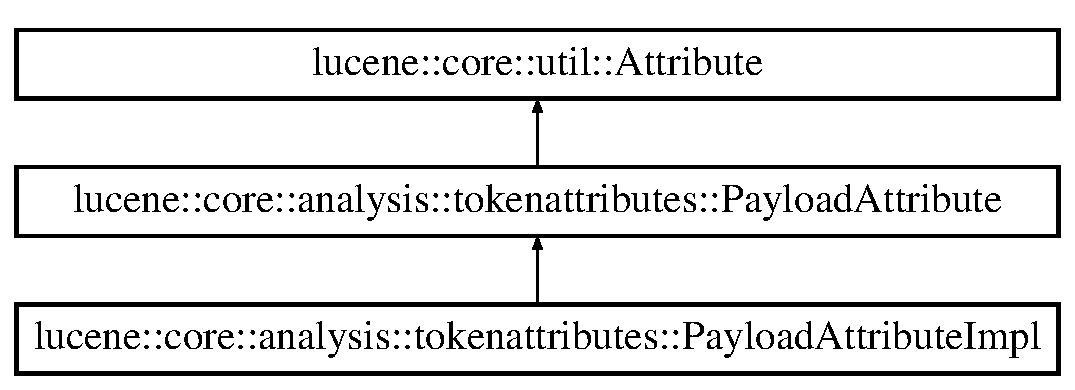
\includegraphics[height=3.000000cm]{classlucene_1_1core_1_1analysis_1_1tokenattributes_1_1PayloadAttribute}
\end{center}
\end{figure}
\subsection*{Public Member Functions}
\begin{DoxyCompactItemize}
\item 
virtual \mbox{\hyperlink{classlucene_1_1core_1_1analysis_1_1tokenattributes_1_1PayloadAttribute_a4211337eb33c29f8dbb035ef9d4db940}{$\sim$\+Payload\+Attribute}} ()
\item 
virtual \mbox{\hyperlink{classlucene_1_1core_1_1util_1_1BytesRef}{lucene\+::core\+::util\+::\+Bytes\+Ref}} \& \mbox{\hyperlink{classlucene_1_1core_1_1analysis_1_1tokenattributes_1_1PayloadAttribute_ad6f64222c371631ce979ba6f7256a11d}{Get\+Payload}} ()=0
\item 
virtual void \mbox{\hyperlink{classlucene_1_1core_1_1analysis_1_1tokenattributes_1_1PayloadAttribute_a52bb5ae9332ad24a12be66374e1f1bcb}{Set\+Payload}} (\mbox{\hyperlink{classlucene_1_1core_1_1util_1_1BytesRef}{lucene\+::core\+::util\+::\+Bytes\+Ref}} \&payload)=0
\end{DoxyCompactItemize}
\subsection*{Additional Inherited Members}


\subsection{Constructor \& Destructor Documentation}
\mbox{\Hypertarget{classlucene_1_1core_1_1analysis_1_1tokenattributes_1_1PayloadAttribute_a4211337eb33c29f8dbb035ef9d4db940}\label{classlucene_1_1core_1_1analysis_1_1tokenattributes_1_1PayloadAttribute_a4211337eb33c29f8dbb035ef9d4db940}} 
\index{lucene\+::core\+::analysis\+::tokenattributes\+::\+Payload\+Attribute@{lucene\+::core\+::analysis\+::tokenattributes\+::\+Payload\+Attribute}!````~Payload\+Attribute@{$\sim$\+Payload\+Attribute}}
\index{````~Payload\+Attribute@{$\sim$\+Payload\+Attribute}!lucene\+::core\+::analysis\+::tokenattributes\+::\+Payload\+Attribute@{lucene\+::core\+::analysis\+::tokenattributes\+::\+Payload\+Attribute}}
\subsubsection{\texorpdfstring{$\sim$\+Payload\+Attribute()}{~PayloadAttribute()}}
{\footnotesize\ttfamily virtual lucene\+::core\+::analysis\+::tokenattributes\+::\+Payload\+Attribute\+::$\sim$\+Payload\+Attribute (\begin{DoxyParamCaption}{ }\end{DoxyParamCaption})\hspace{0.3cm}{\ttfamily [inline]}, {\ttfamily [virtual]}}



\subsection{Member Function Documentation}
\mbox{\Hypertarget{classlucene_1_1core_1_1analysis_1_1tokenattributes_1_1PayloadAttribute_ad6f64222c371631ce979ba6f7256a11d}\label{classlucene_1_1core_1_1analysis_1_1tokenattributes_1_1PayloadAttribute_ad6f64222c371631ce979ba6f7256a11d}} 
\index{lucene\+::core\+::analysis\+::tokenattributes\+::\+Payload\+Attribute@{lucene\+::core\+::analysis\+::tokenattributes\+::\+Payload\+Attribute}!Get\+Payload@{Get\+Payload}}
\index{Get\+Payload@{Get\+Payload}!lucene\+::core\+::analysis\+::tokenattributes\+::\+Payload\+Attribute@{lucene\+::core\+::analysis\+::tokenattributes\+::\+Payload\+Attribute}}
\subsubsection{\texorpdfstring{Get\+Payload()}{GetPayload()}}
{\footnotesize\ttfamily virtual \mbox{\hyperlink{classlucene_1_1core_1_1util_1_1BytesRef}{lucene\+::core\+::util\+::\+Bytes\+Ref}}\& lucene\+::core\+::analysis\+::tokenattributes\+::\+Payload\+Attribute\+::\+Get\+Payload (\begin{DoxyParamCaption}{ }\end{DoxyParamCaption})\hspace{0.3cm}{\ttfamily [pure virtual]}}



Implemented in \mbox{\hyperlink{classlucene_1_1core_1_1analysis_1_1tokenattributes_1_1PayloadAttributeImpl_a60adf0536ed3492e2cbfc2f59846ff8d}{lucene\+::core\+::analysis\+::tokenattributes\+::\+Payload\+Attribute\+Impl}}.

\mbox{\Hypertarget{classlucene_1_1core_1_1analysis_1_1tokenattributes_1_1PayloadAttribute_a52bb5ae9332ad24a12be66374e1f1bcb}\label{classlucene_1_1core_1_1analysis_1_1tokenattributes_1_1PayloadAttribute_a52bb5ae9332ad24a12be66374e1f1bcb}} 
\index{lucene\+::core\+::analysis\+::tokenattributes\+::\+Payload\+Attribute@{lucene\+::core\+::analysis\+::tokenattributes\+::\+Payload\+Attribute}!Set\+Payload@{Set\+Payload}}
\index{Set\+Payload@{Set\+Payload}!lucene\+::core\+::analysis\+::tokenattributes\+::\+Payload\+Attribute@{lucene\+::core\+::analysis\+::tokenattributes\+::\+Payload\+Attribute}}
\subsubsection{\texorpdfstring{Set\+Payload()}{SetPayload()}}
{\footnotesize\ttfamily virtual void lucene\+::core\+::analysis\+::tokenattributes\+::\+Payload\+Attribute\+::\+Set\+Payload (\begin{DoxyParamCaption}\item[{\mbox{\hyperlink{classlucene_1_1core_1_1util_1_1BytesRef}{lucene\+::core\+::util\+::\+Bytes\+Ref}} \&}]{payload }\end{DoxyParamCaption})\hspace{0.3cm}{\ttfamily [pure virtual]}}



Implemented in \mbox{\hyperlink{classlucene_1_1core_1_1analysis_1_1tokenattributes_1_1PayloadAttributeImpl_a69b9a7d6938f53e84dff76d6a0e9c2f3}{lucene\+::core\+::analysis\+::tokenattributes\+::\+Payload\+Attribute\+Impl}}.



The documentation for this class was generated from the following file\+:\begin{DoxyCompactItemize}
\item 
Analysis/\mbox{\hyperlink{Analysis_2Attribute_8h}{Attribute.\+h}}\end{DoxyCompactItemize}

\hypertarget{classlucene_1_1core_1_1analysis_1_1tokenattributes_1_1PayloadAttributeImpl}{}\section{lucene\+:\+:core\+:\+:analysis\+:\+:tokenattributes\+:\+:Payload\+Attribute\+Impl Class Reference}
\label{classlucene_1_1core_1_1analysis_1_1tokenattributes_1_1PayloadAttributeImpl}\index{lucene\+::core\+::analysis\+::tokenattributes\+::\+Payload\+Attribute\+Impl@{lucene\+::core\+::analysis\+::tokenattributes\+::\+Payload\+Attribute\+Impl}}


{\ttfamily \#include $<$Attribute\+Impl.\+h$>$}

Inheritance diagram for lucene\+:\+:core\+:\+:analysis\+:\+:tokenattributes\+:\+:Payload\+Attribute\+Impl\+:\begin{figure}[H]
\begin{center}
\leavevmode
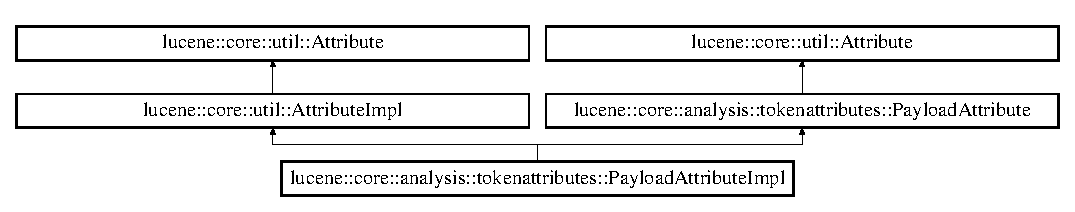
\includegraphics[height=2.400000cm]{classlucene_1_1core_1_1analysis_1_1tokenattributes_1_1PayloadAttributeImpl}
\end{center}
\end{figure}
\subsection*{Public Member Functions}
\begin{DoxyCompactItemize}
\item 
\mbox{\hyperlink{classlucene_1_1core_1_1analysis_1_1tokenattributes_1_1PayloadAttributeImpl_a3f2e143ad91331fdb3123171aeba2b5b}{Payload\+Attribute\+Impl}} ()
\item 
\mbox{\hyperlink{classlucene_1_1core_1_1analysis_1_1tokenattributes_1_1PayloadAttributeImpl_ab110d44b86e2a332642d5b9f3166ef48}{Payload\+Attribute\+Impl}} (\mbox{\hyperlink{ZlibCrc32_8h_a2c212835823e3c54a8ab6d95c652660e}{const}} \mbox{\hyperlink{classlucene_1_1core_1_1analysis_1_1tokenattributes_1_1PayloadAttributeImpl}{Payload\+Attribute\+Impl}} \&other)
\item 
virtual \mbox{\hyperlink{classlucene_1_1core_1_1analysis_1_1tokenattributes_1_1PayloadAttributeImpl_a03a337d859f174328c1b92ee46daf42c}{$\sim$\+Payload\+Attribute\+Impl}} ()
\item 
void \mbox{\hyperlink{classlucene_1_1core_1_1analysis_1_1tokenattributes_1_1PayloadAttributeImpl_ab012363b8b4ce7e15c9c91ba6ec0c325}{Reflect\+With}} (\mbox{\hyperlink{namespacelucene_1_1core_1_1util_a7dbb701adaed055f73fb95eec83da10a}{lucene\+::core\+::util\+::\+Attribute\+Reflector}} \&reflector) override
\item 
void \mbox{\hyperlink{classlucene_1_1core_1_1analysis_1_1tokenattributes_1_1PayloadAttributeImpl_a264f13a218ec4caca8c724e3c34f64b6}{Clear}} () override
\item 
bool \mbox{\hyperlink{classlucene_1_1core_1_1analysis_1_1tokenattributes_1_1PayloadAttributeImpl_a2022641a26ad34c34b75cf47caf2f223}{operator==}} (\mbox{\hyperlink{ZlibCrc32_8h_a2c212835823e3c54a8ab6d95c652660e}{const}} \mbox{\hyperlink{classlucene_1_1core_1_1analysis_1_1tokenattributes_1_1PayloadAttributeImpl}{Payload\+Attribute\+Impl}} \&other) \mbox{\hyperlink{ZlibCrc32_8h_a2c212835823e3c54a8ab6d95c652660e}{const}}
\item 
\mbox{\hyperlink{classlucene_1_1core_1_1util_1_1BytesRef}{lucene\+::core\+::util\+::\+Bytes\+Ref}} \& \mbox{\hyperlink{classlucene_1_1core_1_1analysis_1_1tokenattributes_1_1PayloadAttributeImpl_a60adf0536ed3492e2cbfc2f59846ff8d}{Get\+Payload}} () override
\item 
void \mbox{\hyperlink{classlucene_1_1core_1_1analysis_1_1tokenattributes_1_1PayloadAttributeImpl_a69b9a7d6938f53e84dff76d6a0e9c2f3}{Set\+Payload}} (\mbox{\hyperlink{classlucene_1_1core_1_1util_1_1BytesRef}{lucene\+::core\+::util\+::\+Bytes\+Ref}} \&\mbox{\hyperlink{classlucene_1_1core_1_1analysis_1_1tokenattributes_1_1PayloadAttributeImpl_ac5bd28a25a555ffb21b75fda1036def1}{payload}}) override
\item 
std\+::vector$<$ std\+::type\+\_\+index $>$ \mbox{\hyperlink{classlucene_1_1core_1_1analysis_1_1tokenattributes_1_1PayloadAttributeImpl_a1f7dbb8afdd42ca827dc6e077445071b}{Attributes}} () override
\item 
void \mbox{\hyperlink{classlucene_1_1core_1_1analysis_1_1tokenattributes_1_1PayloadAttributeImpl_ae1104df0b599fd494620e2bce9d39b6c}{Shallow\+Copy\+To}} (\mbox{\hyperlink{classlucene_1_1core_1_1util_1_1AttributeImpl}{lucene\+::core\+::util\+::\+Attribute\+Impl}} \&attr\+\_\+impl) override
\item 
\mbox{\hyperlink{classlucene_1_1core_1_1analysis_1_1tokenattributes_1_1PayloadAttributeImpl}{Payload\+Attribute\+Impl}} \& \mbox{\hyperlink{classlucene_1_1core_1_1analysis_1_1tokenattributes_1_1PayloadAttributeImpl_a82dd546c2275107d47d6a152cd43d04e}{operator=}} (\mbox{\hyperlink{ZlibCrc32_8h_a2c212835823e3c54a8ab6d95c652660e}{const}} \mbox{\hyperlink{classlucene_1_1core_1_1util_1_1AttributeImpl}{lucene\+::core\+::util\+::\+Attribute\+Impl}} \&other)
\item 
\mbox{\hyperlink{classlucene_1_1core_1_1analysis_1_1tokenattributes_1_1PayloadAttributeImpl}{Payload\+Attribute\+Impl}} \& \mbox{\hyperlink{classlucene_1_1core_1_1analysis_1_1tokenattributes_1_1PayloadAttributeImpl_ac5a8e038064f6ee8774df0708467201f}{operator=}} (\mbox{\hyperlink{ZlibCrc32_8h_a2c212835823e3c54a8ab6d95c652660e}{const}} \mbox{\hyperlink{classlucene_1_1core_1_1analysis_1_1tokenattributes_1_1PayloadAttributeImpl}{Payload\+Attribute\+Impl}} \&other)
\item 
\mbox{\hyperlink{classlucene_1_1core_1_1util_1_1AttributeImpl}{lucene\+::core\+::util\+::\+Attribute\+Impl}} $\ast$ \mbox{\hyperlink{classlucene_1_1core_1_1analysis_1_1tokenattributes_1_1PayloadAttributeImpl_a5ec30ffd50c79e22ba0166b0e47629b3}{Clone}} () override
\end{DoxyCompactItemize}
\subsection*{Private Attributes}
\begin{DoxyCompactItemize}
\item 
\mbox{\hyperlink{classlucene_1_1core_1_1util_1_1BytesRef}{lucene\+::core\+::util\+::\+Bytes\+Ref}} \mbox{\hyperlink{classlucene_1_1core_1_1analysis_1_1tokenattributes_1_1PayloadAttributeImpl_ac5bd28a25a555ffb21b75fda1036def1}{payload}}
\end{DoxyCompactItemize}
\subsection*{Additional Inherited Members}


\subsection{Constructor \& Destructor Documentation}
\mbox{\Hypertarget{classlucene_1_1core_1_1analysis_1_1tokenattributes_1_1PayloadAttributeImpl_a3f2e143ad91331fdb3123171aeba2b5b}\label{classlucene_1_1core_1_1analysis_1_1tokenattributes_1_1PayloadAttributeImpl_a3f2e143ad91331fdb3123171aeba2b5b}} 
\index{lucene\+::core\+::analysis\+::tokenattributes\+::\+Payload\+Attribute\+Impl@{lucene\+::core\+::analysis\+::tokenattributes\+::\+Payload\+Attribute\+Impl}!Payload\+Attribute\+Impl@{Payload\+Attribute\+Impl}}
\index{Payload\+Attribute\+Impl@{Payload\+Attribute\+Impl}!lucene\+::core\+::analysis\+::tokenattributes\+::\+Payload\+Attribute\+Impl@{lucene\+::core\+::analysis\+::tokenattributes\+::\+Payload\+Attribute\+Impl}}
\subsubsection{\texorpdfstring{Payload\+Attribute\+Impl()}{PayloadAttributeImpl()}\hspace{0.1cm}{\footnotesize\ttfamily [1/2]}}
{\footnotesize\ttfamily Payload\+Attribute\+Impl\+::\+Payload\+Attribute\+Impl (\begin{DoxyParamCaption}{ }\end{DoxyParamCaption})}

\mbox{\hyperlink{classlucene_1_1core_1_1analysis_1_1tokenattributes_1_1PayloadAttributeImpl}{Payload\+Attribute\+Impl}} \mbox{\Hypertarget{classlucene_1_1core_1_1analysis_1_1tokenattributes_1_1PayloadAttributeImpl_ab110d44b86e2a332642d5b9f3166ef48}\label{classlucene_1_1core_1_1analysis_1_1tokenattributes_1_1PayloadAttributeImpl_ab110d44b86e2a332642d5b9f3166ef48}} 
\index{lucene\+::core\+::analysis\+::tokenattributes\+::\+Payload\+Attribute\+Impl@{lucene\+::core\+::analysis\+::tokenattributes\+::\+Payload\+Attribute\+Impl}!Payload\+Attribute\+Impl@{Payload\+Attribute\+Impl}}
\index{Payload\+Attribute\+Impl@{Payload\+Attribute\+Impl}!lucene\+::core\+::analysis\+::tokenattributes\+::\+Payload\+Attribute\+Impl@{lucene\+::core\+::analysis\+::tokenattributes\+::\+Payload\+Attribute\+Impl}}
\subsubsection{\texorpdfstring{Payload\+Attribute\+Impl()}{PayloadAttributeImpl()}\hspace{0.1cm}{\footnotesize\ttfamily [2/2]}}
{\footnotesize\ttfamily Payload\+Attribute\+Impl\+::\+Payload\+Attribute\+Impl (\begin{DoxyParamCaption}\item[{\mbox{\hyperlink{ZlibCrc32_8h_a2c212835823e3c54a8ab6d95c652660e}{const}} \mbox{\hyperlink{classlucene_1_1core_1_1analysis_1_1tokenattributes_1_1PayloadAttributeImpl}{Payload\+Attribute\+Impl}} \&}]{other }\end{DoxyParamCaption})}

\mbox{\Hypertarget{classlucene_1_1core_1_1analysis_1_1tokenattributes_1_1PayloadAttributeImpl_a03a337d859f174328c1b92ee46daf42c}\label{classlucene_1_1core_1_1analysis_1_1tokenattributes_1_1PayloadAttributeImpl_a03a337d859f174328c1b92ee46daf42c}} 
\index{lucene\+::core\+::analysis\+::tokenattributes\+::\+Payload\+Attribute\+Impl@{lucene\+::core\+::analysis\+::tokenattributes\+::\+Payload\+Attribute\+Impl}!````~Payload\+Attribute\+Impl@{$\sim$\+Payload\+Attribute\+Impl}}
\index{````~Payload\+Attribute\+Impl@{$\sim$\+Payload\+Attribute\+Impl}!lucene\+::core\+::analysis\+::tokenattributes\+::\+Payload\+Attribute\+Impl@{lucene\+::core\+::analysis\+::tokenattributes\+::\+Payload\+Attribute\+Impl}}
\subsubsection{\texorpdfstring{$\sim$\+Payload\+Attribute\+Impl()}{~PayloadAttributeImpl()}}
{\footnotesize\ttfamily Payload\+Attribute\+Impl\+::$\sim$\+Payload\+Attribute\+Impl (\begin{DoxyParamCaption}{ }\end{DoxyParamCaption})\hspace{0.3cm}{\ttfamily [virtual]}}



\subsection{Member Function Documentation}
\mbox{\Hypertarget{classlucene_1_1core_1_1analysis_1_1tokenattributes_1_1PayloadAttributeImpl_a1f7dbb8afdd42ca827dc6e077445071b}\label{classlucene_1_1core_1_1analysis_1_1tokenattributes_1_1PayloadAttributeImpl_a1f7dbb8afdd42ca827dc6e077445071b}} 
\index{lucene\+::core\+::analysis\+::tokenattributes\+::\+Payload\+Attribute\+Impl@{lucene\+::core\+::analysis\+::tokenattributes\+::\+Payload\+Attribute\+Impl}!Attributes@{Attributes}}
\index{Attributes@{Attributes}!lucene\+::core\+::analysis\+::tokenattributes\+::\+Payload\+Attribute\+Impl@{lucene\+::core\+::analysis\+::tokenattributes\+::\+Payload\+Attribute\+Impl}}
\subsubsection{\texorpdfstring{Attributes()}{Attributes()}}
{\footnotesize\ttfamily std\+::vector$<$ std\+::type\+\_\+index $>$ Payload\+Attribute\+Impl\+::\+Attributes (\begin{DoxyParamCaption}{ }\end{DoxyParamCaption})\hspace{0.3cm}{\ttfamily [override]}, {\ttfamily [virtual]}}



Implements \mbox{\hyperlink{classlucene_1_1core_1_1util_1_1AttributeImpl_ac0631e6a7a11044883bc97447716d7cc}{lucene\+::core\+::util\+::\+Attribute\+Impl}}.

\mbox{\Hypertarget{classlucene_1_1core_1_1analysis_1_1tokenattributes_1_1PayloadAttributeImpl_a264f13a218ec4caca8c724e3c34f64b6}\label{classlucene_1_1core_1_1analysis_1_1tokenattributes_1_1PayloadAttributeImpl_a264f13a218ec4caca8c724e3c34f64b6}} 
\index{lucene\+::core\+::analysis\+::tokenattributes\+::\+Payload\+Attribute\+Impl@{lucene\+::core\+::analysis\+::tokenattributes\+::\+Payload\+Attribute\+Impl}!Clear@{Clear}}
\index{Clear@{Clear}!lucene\+::core\+::analysis\+::tokenattributes\+::\+Payload\+Attribute\+Impl@{lucene\+::core\+::analysis\+::tokenattributes\+::\+Payload\+Attribute\+Impl}}
\subsubsection{\texorpdfstring{Clear()}{Clear()}}
{\footnotesize\ttfamily void Payload\+Attribute\+Impl\+::\+Clear (\begin{DoxyParamCaption}{ }\end{DoxyParamCaption})\hspace{0.3cm}{\ttfamily [override]}, {\ttfamily [virtual]}}



Implements \mbox{\hyperlink{classlucene_1_1core_1_1util_1_1AttributeImpl_a04897a00a902f7a345dd44bbc4b482a8}{lucene\+::core\+::util\+::\+Attribute\+Impl}}.

\mbox{\Hypertarget{classlucene_1_1core_1_1analysis_1_1tokenattributes_1_1PayloadAttributeImpl_a5ec30ffd50c79e22ba0166b0e47629b3}\label{classlucene_1_1core_1_1analysis_1_1tokenattributes_1_1PayloadAttributeImpl_a5ec30ffd50c79e22ba0166b0e47629b3}} 
\index{lucene\+::core\+::analysis\+::tokenattributes\+::\+Payload\+Attribute\+Impl@{lucene\+::core\+::analysis\+::tokenattributes\+::\+Payload\+Attribute\+Impl}!Clone@{Clone}}
\index{Clone@{Clone}!lucene\+::core\+::analysis\+::tokenattributes\+::\+Payload\+Attribute\+Impl@{lucene\+::core\+::analysis\+::tokenattributes\+::\+Payload\+Attribute\+Impl}}
\subsubsection{\texorpdfstring{Clone()}{Clone()}}
{\footnotesize\ttfamily \mbox{\hyperlink{classlucene_1_1core_1_1util_1_1AttributeImpl}{Attribute\+Impl}} $\ast$ Payload\+Attribute\+Impl\+::\+Clone (\begin{DoxyParamCaption}{ }\end{DoxyParamCaption})\hspace{0.3cm}{\ttfamily [override]}, {\ttfamily [virtual]}}



Implements \mbox{\hyperlink{classlucene_1_1core_1_1util_1_1AttributeImpl_a135318ad4c7c17b3d85e625e32fb42cd}{lucene\+::core\+::util\+::\+Attribute\+Impl}}.

\mbox{\Hypertarget{classlucene_1_1core_1_1analysis_1_1tokenattributes_1_1PayloadAttributeImpl_a60adf0536ed3492e2cbfc2f59846ff8d}\label{classlucene_1_1core_1_1analysis_1_1tokenattributes_1_1PayloadAttributeImpl_a60adf0536ed3492e2cbfc2f59846ff8d}} 
\index{lucene\+::core\+::analysis\+::tokenattributes\+::\+Payload\+Attribute\+Impl@{lucene\+::core\+::analysis\+::tokenattributes\+::\+Payload\+Attribute\+Impl}!Get\+Payload@{Get\+Payload}}
\index{Get\+Payload@{Get\+Payload}!lucene\+::core\+::analysis\+::tokenattributes\+::\+Payload\+Attribute\+Impl@{lucene\+::core\+::analysis\+::tokenattributes\+::\+Payload\+Attribute\+Impl}}
\subsubsection{\texorpdfstring{Get\+Payload()}{GetPayload()}}
{\footnotesize\ttfamily \mbox{\hyperlink{classlucene_1_1core_1_1util_1_1BytesRef}{Bytes\+Ref}} \& Payload\+Attribute\+Impl\+::\+Get\+Payload (\begin{DoxyParamCaption}{ }\end{DoxyParamCaption})\hspace{0.3cm}{\ttfamily [override]}, {\ttfamily [virtual]}}



Implements \mbox{\hyperlink{classlucene_1_1core_1_1analysis_1_1tokenattributes_1_1PayloadAttribute_ad6f64222c371631ce979ba6f7256a11d}{lucene\+::core\+::analysis\+::tokenattributes\+::\+Payload\+Attribute}}.

\mbox{\Hypertarget{classlucene_1_1core_1_1analysis_1_1tokenattributes_1_1PayloadAttributeImpl_a82dd546c2275107d47d6a152cd43d04e}\label{classlucene_1_1core_1_1analysis_1_1tokenattributes_1_1PayloadAttributeImpl_a82dd546c2275107d47d6a152cd43d04e}} 
\index{lucene\+::core\+::analysis\+::tokenattributes\+::\+Payload\+Attribute\+Impl@{lucene\+::core\+::analysis\+::tokenattributes\+::\+Payload\+Attribute\+Impl}!operator=@{operator=}}
\index{operator=@{operator=}!lucene\+::core\+::analysis\+::tokenattributes\+::\+Payload\+Attribute\+Impl@{lucene\+::core\+::analysis\+::tokenattributes\+::\+Payload\+Attribute\+Impl}}
\subsubsection{\texorpdfstring{operator=()}{operator=()}\hspace{0.1cm}{\footnotesize\ttfamily [1/2]}}
{\footnotesize\ttfamily \mbox{\hyperlink{classlucene_1_1core_1_1analysis_1_1tokenattributes_1_1PayloadAttributeImpl}{Payload\+Attribute\+Impl}} \& Payload\+Attribute\+Impl\+::operator= (\begin{DoxyParamCaption}\item[{\mbox{\hyperlink{ZlibCrc32_8h_a2c212835823e3c54a8ab6d95c652660e}{const}} \mbox{\hyperlink{classlucene_1_1core_1_1util_1_1AttributeImpl}{lucene\+::core\+::util\+::\+Attribute\+Impl}} \&}]{other }\end{DoxyParamCaption})\hspace{0.3cm}{\ttfamily [virtual]}}



Implements \mbox{\hyperlink{classlucene_1_1core_1_1util_1_1AttributeImpl_ab032e399d03ce2f58c76881cf2b92325}{lucene\+::core\+::util\+::\+Attribute\+Impl}}.

\mbox{\Hypertarget{classlucene_1_1core_1_1analysis_1_1tokenattributes_1_1PayloadAttributeImpl_ac5a8e038064f6ee8774df0708467201f}\label{classlucene_1_1core_1_1analysis_1_1tokenattributes_1_1PayloadAttributeImpl_ac5a8e038064f6ee8774df0708467201f}} 
\index{lucene\+::core\+::analysis\+::tokenattributes\+::\+Payload\+Attribute\+Impl@{lucene\+::core\+::analysis\+::tokenattributes\+::\+Payload\+Attribute\+Impl}!operator=@{operator=}}
\index{operator=@{operator=}!lucene\+::core\+::analysis\+::tokenattributes\+::\+Payload\+Attribute\+Impl@{lucene\+::core\+::analysis\+::tokenattributes\+::\+Payload\+Attribute\+Impl}}
\subsubsection{\texorpdfstring{operator=()}{operator=()}\hspace{0.1cm}{\footnotesize\ttfamily [2/2]}}
{\footnotesize\ttfamily \mbox{\hyperlink{classlucene_1_1core_1_1analysis_1_1tokenattributes_1_1PayloadAttributeImpl}{Payload\+Attribute\+Impl}} \& Payload\+Attribute\+Impl\+::operator= (\begin{DoxyParamCaption}\item[{\mbox{\hyperlink{ZlibCrc32_8h_a2c212835823e3c54a8ab6d95c652660e}{const}} \mbox{\hyperlink{classlucene_1_1core_1_1analysis_1_1tokenattributes_1_1PayloadAttributeImpl}{Payload\+Attribute\+Impl}} \&}]{other }\end{DoxyParamCaption})}

\mbox{\Hypertarget{classlucene_1_1core_1_1analysis_1_1tokenattributes_1_1PayloadAttributeImpl_a2022641a26ad34c34b75cf47caf2f223}\label{classlucene_1_1core_1_1analysis_1_1tokenattributes_1_1PayloadAttributeImpl_a2022641a26ad34c34b75cf47caf2f223}} 
\index{lucene\+::core\+::analysis\+::tokenattributes\+::\+Payload\+Attribute\+Impl@{lucene\+::core\+::analysis\+::tokenattributes\+::\+Payload\+Attribute\+Impl}!operator==@{operator==}}
\index{operator==@{operator==}!lucene\+::core\+::analysis\+::tokenattributes\+::\+Payload\+Attribute\+Impl@{lucene\+::core\+::analysis\+::tokenattributes\+::\+Payload\+Attribute\+Impl}}
\subsubsection{\texorpdfstring{operator==()}{operator==()}}
{\footnotesize\ttfamily bool Payload\+Attribute\+Impl\+::operator== (\begin{DoxyParamCaption}\item[{\mbox{\hyperlink{ZlibCrc32_8h_a2c212835823e3c54a8ab6d95c652660e}{const}} \mbox{\hyperlink{classlucene_1_1core_1_1analysis_1_1tokenattributes_1_1PayloadAttributeImpl}{Payload\+Attribute\+Impl}} \&}]{other }\end{DoxyParamCaption}) const}

\mbox{\Hypertarget{classlucene_1_1core_1_1analysis_1_1tokenattributes_1_1PayloadAttributeImpl_ab012363b8b4ce7e15c9c91ba6ec0c325}\label{classlucene_1_1core_1_1analysis_1_1tokenattributes_1_1PayloadAttributeImpl_ab012363b8b4ce7e15c9c91ba6ec0c325}} 
\index{lucene\+::core\+::analysis\+::tokenattributes\+::\+Payload\+Attribute\+Impl@{lucene\+::core\+::analysis\+::tokenattributes\+::\+Payload\+Attribute\+Impl}!Reflect\+With@{Reflect\+With}}
\index{Reflect\+With@{Reflect\+With}!lucene\+::core\+::analysis\+::tokenattributes\+::\+Payload\+Attribute\+Impl@{lucene\+::core\+::analysis\+::tokenattributes\+::\+Payload\+Attribute\+Impl}}
\subsubsection{\texorpdfstring{Reflect\+With()}{ReflectWith()}}
{\footnotesize\ttfamily void Payload\+Attribute\+Impl\+::\+Reflect\+With (\begin{DoxyParamCaption}\item[{\mbox{\hyperlink{namespacelucene_1_1core_1_1util_a7dbb701adaed055f73fb95eec83da10a}{lucene\+::core\+::util\+::\+Attribute\+Reflector}} \&}]{reflector }\end{DoxyParamCaption})\hspace{0.3cm}{\ttfamily [override]}, {\ttfamily [virtual]}}



Implements \mbox{\hyperlink{classlucene_1_1core_1_1util_1_1AttributeImpl_a84d34275fb1ed67ac36fad7ff6388096}{lucene\+::core\+::util\+::\+Attribute\+Impl}}.

\mbox{\Hypertarget{classlucene_1_1core_1_1analysis_1_1tokenattributes_1_1PayloadAttributeImpl_a69b9a7d6938f53e84dff76d6a0e9c2f3}\label{classlucene_1_1core_1_1analysis_1_1tokenattributes_1_1PayloadAttributeImpl_a69b9a7d6938f53e84dff76d6a0e9c2f3}} 
\index{lucene\+::core\+::analysis\+::tokenattributes\+::\+Payload\+Attribute\+Impl@{lucene\+::core\+::analysis\+::tokenattributes\+::\+Payload\+Attribute\+Impl}!Set\+Payload@{Set\+Payload}}
\index{Set\+Payload@{Set\+Payload}!lucene\+::core\+::analysis\+::tokenattributes\+::\+Payload\+Attribute\+Impl@{lucene\+::core\+::analysis\+::tokenattributes\+::\+Payload\+Attribute\+Impl}}
\subsubsection{\texorpdfstring{Set\+Payload()}{SetPayload()}}
{\footnotesize\ttfamily void Payload\+Attribute\+Impl\+::\+Set\+Payload (\begin{DoxyParamCaption}\item[{\mbox{\hyperlink{classlucene_1_1core_1_1util_1_1BytesRef}{lucene\+::core\+::util\+::\+Bytes\+Ref}} \&}]{payload }\end{DoxyParamCaption})\hspace{0.3cm}{\ttfamily [override]}, {\ttfamily [virtual]}}



Implements \mbox{\hyperlink{classlucene_1_1core_1_1analysis_1_1tokenattributes_1_1PayloadAttribute_a52bb5ae9332ad24a12be66374e1f1bcb}{lucene\+::core\+::analysis\+::tokenattributes\+::\+Payload\+Attribute}}.

\mbox{\Hypertarget{classlucene_1_1core_1_1analysis_1_1tokenattributes_1_1PayloadAttributeImpl_ae1104df0b599fd494620e2bce9d39b6c}\label{classlucene_1_1core_1_1analysis_1_1tokenattributes_1_1PayloadAttributeImpl_ae1104df0b599fd494620e2bce9d39b6c}} 
\index{lucene\+::core\+::analysis\+::tokenattributes\+::\+Payload\+Attribute\+Impl@{lucene\+::core\+::analysis\+::tokenattributes\+::\+Payload\+Attribute\+Impl}!Shallow\+Copy\+To@{Shallow\+Copy\+To}}
\index{Shallow\+Copy\+To@{Shallow\+Copy\+To}!lucene\+::core\+::analysis\+::tokenattributes\+::\+Payload\+Attribute\+Impl@{lucene\+::core\+::analysis\+::tokenattributes\+::\+Payload\+Attribute\+Impl}}
\subsubsection{\texorpdfstring{Shallow\+Copy\+To()}{ShallowCopyTo()}}
{\footnotesize\ttfamily void Payload\+Attribute\+Impl\+::\+Shallow\+Copy\+To (\begin{DoxyParamCaption}\item[{\mbox{\hyperlink{classlucene_1_1core_1_1util_1_1AttributeImpl}{lucene\+::core\+::util\+::\+Attribute\+Impl}} \&}]{attr\+\_\+impl }\end{DoxyParamCaption})\hspace{0.3cm}{\ttfamily [override]}, {\ttfamily [virtual]}}



Implements \mbox{\hyperlink{classlucene_1_1core_1_1util_1_1AttributeImpl_a010e8937832f53139c8fe42757476895}{lucene\+::core\+::util\+::\+Attribute\+Impl}}.



\subsection{Member Data Documentation}
\mbox{\Hypertarget{classlucene_1_1core_1_1analysis_1_1tokenattributes_1_1PayloadAttributeImpl_ac5bd28a25a555ffb21b75fda1036def1}\label{classlucene_1_1core_1_1analysis_1_1tokenattributes_1_1PayloadAttributeImpl_ac5bd28a25a555ffb21b75fda1036def1}} 
\index{lucene\+::core\+::analysis\+::tokenattributes\+::\+Payload\+Attribute\+Impl@{lucene\+::core\+::analysis\+::tokenattributes\+::\+Payload\+Attribute\+Impl}!payload@{payload}}
\index{payload@{payload}!lucene\+::core\+::analysis\+::tokenattributes\+::\+Payload\+Attribute\+Impl@{lucene\+::core\+::analysis\+::tokenattributes\+::\+Payload\+Attribute\+Impl}}
\subsubsection{\texorpdfstring{payload}{payload}}
{\footnotesize\ttfamily \mbox{\hyperlink{classlucene_1_1core_1_1util_1_1BytesRef}{lucene\+::core\+::util\+::\+Bytes\+Ref}} lucene\+::core\+::analysis\+::tokenattributes\+::\+Payload\+Attribute\+Impl\+::payload\hspace{0.3cm}{\ttfamily [private]}}



The documentation for this class was generated from the following files\+:\begin{DoxyCompactItemize}
\item 
Analysis/\mbox{\hyperlink{AttributeImpl_8h}{Attribute\+Impl.\+h}}\item 
Analysis/\mbox{\hyperlink{AttributeImpl_8cpp}{Attribute\+Impl.\+cpp}}\end{DoxyCompactItemize}

\hypertarget{classlucene_1_1core_1_1analysis_1_1PerFieldReuseStrategy}{}\section{lucene\+:\+:core\+:\+:analysis\+:\+:Per\+Field\+Reuse\+Strategy Class Reference}
\label{classlucene_1_1core_1_1analysis_1_1PerFieldReuseStrategy}\index{lucene\+::core\+::analysis\+::\+Per\+Field\+Reuse\+Strategy@{lucene\+::core\+::analysis\+::\+Per\+Field\+Reuse\+Strategy}}


{\ttfamily \#include $<$Analyzer.\+h$>$}

Inheritance diagram for lucene\+:\+:core\+:\+:analysis\+:\+:Per\+Field\+Reuse\+Strategy\+:\begin{figure}[H]
\begin{center}
\leavevmode
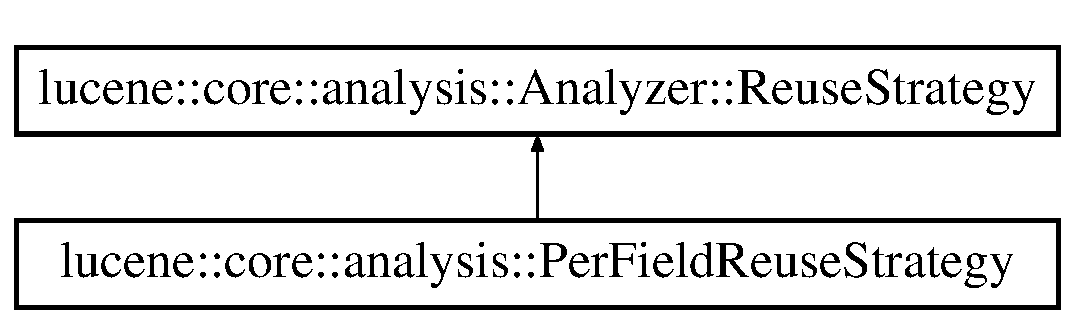
\includegraphics[height=2.000000cm]{classlucene_1_1core_1_1analysis_1_1PerFieldReuseStrategy}
\end{center}
\end{figure}
\subsection*{Public Member Functions}
\begin{DoxyCompactItemize}
\item 
\mbox{\hyperlink{classlucene_1_1core_1_1analysis_1_1PerFieldReuseStrategy_ab2081194878f10803b28ff228db7327c}{Per\+Field\+Reuse\+Strategy}} ()
\item 
virtual \mbox{\hyperlink{classlucene_1_1core_1_1analysis_1_1PerFieldReuseStrategy_ab5af1cea75460e48364696c8a89bdbeb}{$\sim$\+Per\+Field\+Reuse\+Strategy}} ()
\item 
\mbox{\hyperlink{classlucene_1_1core_1_1analysis_1_1TokenStreamComponents}{Token\+Stream\+Components}} $\ast$ \mbox{\hyperlink{classlucene_1_1core_1_1analysis_1_1PerFieldReuseStrategy_ab0d86155823842bb28e43bbbec7c06d3}{Get\+Reusable\+Components}} (\mbox{\hyperlink{classlucene_1_1core_1_1analysis_1_1Analyzer}{Analyzer}} \&analyzer, const std\+::string \&field\+\_\+name) override
\item 
void \mbox{\hyperlink{classlucene_1_1core_1_1analysis_1_1PerFieldReuseStrategy_ab23b95640469c639fd36ac888eeda1c3}{Set\+Reusable\+Components}} (\mbox{\hyperlink{classlucene_1_1core_1_1analysis_1_1Analyzer}{Analyzer}} \&analyzer, const std\+::string \&field\+\_\+name, \mbox{\hyperlink{classlucene_1_1core_1_1analysis_1_1TokenStreamComponents}{Token\+Stream\+Components}} $\ast$components) override
\end{DoxyCompactItemize}
\subsection*{Private Attributes}
\begin{DoxyCompactItemize}
\item 
\mbox{\hyperlink{classlucene_1_1core_1_1util_1_1CloseableThreadLocal}{lucene\+::core\+::util\+::\+Closeable\+Thread\+Local}}$<$ \mbox{\hyperlink{classlucene_1_1core_1_1analysis_1_1PerFieldReuseStrategy}{Per\+Field\+Reuse\+Strategy}}, std\+::unordered\+\_\+map$<$ std\+::string, std\+::unique\+\_\+ptr$<$ \mbox{\hyperlink{classlucene_1_1core_1_1analysis_1_1TokenStreamComponents}{Token\+Stream\+Components}} $>$ $>$ $>$ \mbox{\hyperlink{classlucene_1_1core_1_1analysis_1_1PerFieldReuseStrategy_a641b5ee9fc538da0504ae9f13438d89e}{stored\+\_\+value}}
\end{DoxyCompactItemize}


\subsection{Constructor \& Destructor Documentation}
\mbox{\Hypertarget{classlucene_1_1core_1_1analysis_1_1PerFieldReuseStrategy_ab2081194878f10803b28ff228db7327c}\label{classlucene_1_1core_1_1analysis_1_1PerFieldReuseStrategy_ab2081194878f10803b28ff228db7327c}} 
\index{lucene\+::core\+::analysis\+::\+Per\+Field\+Reuse\+Strategy@{lucene\+::core\+::analysis\+::\+Per\+Field\+Reuse\+Strategy}!Per\+Field\+Reuse\+Strategy@{Per\+Field\+Reuse\+Strategy}}
\index{Per\+Field\+Reuse\+Strategy@{Per\+Field\+Reuse\+Strategy}!lucene\+::core\+::analysis\+::\+Per\+Field\+Reuse\+Strategy@{lucene\+::core\+::analysis\+::\+Per\+Field\+Reuse\+Strategy}}
\subsubsection{\texorpdfstring{Per\+Field\+Reuse\+Strategy()}{PerFieldReuseStrategy()}}
{\footnotesize\ttfamily Per\+Field\+Reuse\+Strategy\+::\+Per\+Field\+Reuse\+Strategy (\begin{DoxyParamCaption}{ }\end{DoxyParamCaption})}

\mbox{\hyperlink{classlucene_1_1core_1_1analysis_1_1PerFieldReuseStrategy}{Per\+Field\+Reuse\+Strategy}} \mbox{\Hypertarget{classlucene_1_1core_1_1analysis_1_1PerFieldReuseStrategy_ab5af1cea75460e48364696c8a89bdbeb}\label{classlucene_1_1core_1_1analysis_1_1PerFieldReuseStrategy_ab5af1cea75460e48364696c8a89bdbeb}} 
\index{lucene\+::core\+::analysis\+::\+Per\+Field\+Reuse\+Strategy@{lucene\+::core\+::analysis\+::\+Per\+Field\+Reuse\+Strategy}!````~Per\+Field\+Reuse\+Strategy@{$\sim$\+Per\+Field\+Reuse\+Strategy}}
\index{````~Per\+Field\+Reuse\+Strategy@{$\sim$\+Per\+Field\+Reuse\+Strategy}!lucene\+::core\+::analysis\+::\+Per\+Field\+Reuse\+Strategy@{lucene\+::core\+::analysis\+::\+Per\+Field\+Reuse\+Strategy}}
\subsubsection{\texorpdfstring{$\sim$\+Per\+Field\+Reuse\+Strategy()}{~PerFieldReuseStrategy()}}
{\footnotesize\ttfamily Per\+Field\+Reuse\+Strategy\+::$\sim$\+Per\+Field\+Reuse\+Strategy (\begin{DoxyParamCaption}{ }\end{DoxyParamCaption})\hspace{0.3cm}{\ttfamily [virtual]}}



\subsection{Member Function Documentation}
\mbox{\Hypertarget{classlucene_1_1core_1_1analysis_1_1PerFieldReuseStrategy_ab0d86155823842bb28e43bbbec7c06d3}\label{classlucene_1_1core_1_1analysis_1_1PerFieldReuseStrategy_ab0d86155823842bb28e43bbbec7c06d3}} 
\index{lucene\+::core\+::analysis\+::\+Per\+Field\+Reuse\+Strategy@{lucene\+::core\+::analysis\+::\+Per\+Field\+Reuse\+Strategy}!Get\+Reusable\+Components@{Get\+Reusable\+Components}}
\index{Get\+Reusable\+Components@{Get\+Reusable\+Components}!lucene\+::core\+::analysis\+::\+Per\+Field\+Reuse\+Strategy@{lucene\+::core\+::analysis\+::\+Per\+Field\+Reuse\+Strategy}}
\subsubsection{\texorpdfstring{Get\+Reusable\+Components()}{GetReusableComponents()}}
{\footnotesize\ttfamily \mbox{\hyperlink{classlucene_1_1core_1_1analysis_1_1TokenStreamComponents}{Token\+Stream\+Components}} $\ast$ Per\+Field\+Reuse\+Strategy\+::\+Get\+Reusable\+Components (\begin{DoxyParamCaption}\item[{\mbox{\hyperlink{classlucene_1_1core_1_1analysis_1_1Analyzer}{Analyzer}} \&}]{analyzer,  }\item[{const std\+::string \&}]{field\+\_\+name }\end{DoxyParamCaption})\hspace{0.3cm}{\ttfamily [override]}, {\ttfamily [virtual]}}



Implements \mbox{\hyperlink{classlucene_1_1core_1_1analysis_1_1Analyzer_1_1ReuseStrategy_ab180767950f392037e8ddf78c2f11f95}{lucene\+::core\+::analysis\+::\+Analyzer\+::\+Reuse\+Strategy}}.

\mbox{\Hypertarget{classlucene_1_1core_1_1analysis_1_1PerFieldReuseStrategy_ab23b95640469c639fd36ac888eeda1c3}\label{classlucene_1_1core_1_1analysis_1_1PerFieldReuseStrategy_ab23b95640469c639fd36ac888eeda1c3}} 
\index{lucene\+::core\+::analysis\+::\+Per\+Field\+Reuse\+Strategy@{lucene\+::core\+::analysis\+::\+Per\+Field\+Reuse\+Strategy}!Set\+Reusable\+Components@{Set\+Reusable\+Components}}
\index{Set\+Reusable\+Components@{Set\+Reusable\+Components}!lucene\+::core\+::analysis\+::\+Per\+Field\+Reuse\+Strategy@{lucene\+::core\+::analysis\+::\+Per\+Field\+Reuse\+Strategy}}
\subsubsection{\texorpdfstring{Set\+Reusable\+Components()}{SetReusableComponents()}}
{\footnotesize\ttfamily void Per\+Field\+Reuse\+Strategy\+::\+Set\+Reusable\+Components (\begin{DoxyParamCaption}\item[{\mbox{\hyperlink{classlucene_1_1core_1_1analysis_1_1Analyzer}{Analyzer}} \&}]{analyzer,  }\item[{const std\+::string \&}]{field\+\_\+name,  }\item[{\mbox{\hyperlink{classlucene_1_1core_1_1analysis_1_1TokenStreamComponents}{Token\+Stream\+Components}} $\ast$}]{components }\end{DoxyParamCaption})\hspace{0.3cm}{\ttfamily [override]}, {\ttfamily [virtual]}}



Implements \mbox{\hyperlink{classlucene_1_1core_1_1analysis_1_1Analyzer_1_1ReuseStrategy_a78a1328d5564e78e2168169b73094b23}{lucene\+::core\+::analysis\+::\+Analyzer\+::\+Reuse\+Strategy}}.



\subsection{Member Data Documentation}
\mbox{\Hypertarget{classlucene_1_1core_1_1analysis_1_1PerFieldReuseStrategy_a641b5ee9fc538da0504ae9f13438d89e}\label{classlucene_1_1core_1_1analysis_1_1PerFieldReuseStrategy_a641b5ee9fc538da0504ae9f13438d89e}} 
\index{lucene\+::core\+::analysis\+::\+Per\+Field\+Reuse\+Strategy@{lucene\+::core\+::analysis\+::\+Per\+Field\+Reuse\+Strategy}!stored\+\_\+value@{stored\+\_\+value}}
\index{stored\+\_\+value@{stored\+\_\+value}!lucene\+::core\+::analysis\+::\+Per\+Field\+Reuse\+Strategy@{lucene\+::core\+::analysis\+::\+Per\+Field\+Reuse\+Strategy}}
\subsubsection{\texorpdfstring{stored\+\_\+value}{stored\_value}}
{\footnotesize\ttfamily \mbox{\hyperlink{classlucene_1_1core_1_1util_1_1CloseableThreadLocal}{lucene\+::core\+::util\+::\+Closeable\+Thread\+Local}}$<$\mbox{\hyperlink{classlucene_1_1core_1_1analysis_1_1PerFieldReuseStrategy}{Per\+Field\+Reuse\+Strategy}}, std\+::unordered\+\_\+map$<$std\+::string, std\+::unique\+\_\+ptr$<$ \mbox{\hyperlink{classlucene_1_1core_1_1analysis_1_1TokenStreamComponents}{Token\+Stream\+Components}}$>$ $>$ $>$ lucene\+::core\+::analysis\+::\+Per\+Field\+Reuse\+Strategy\+::stored\+\_\+value\hspace{0.3cm}{\ttfamily [private]}}



The documentation for this class was generated from the following files\+:\begin{DoxyCompactItemize}
\item 
Analysis/\mbox{\hyperlink{Analyzer_8h}{Analyzer.\+h}}\item 
Analysis/\mbox{\hyperlink{Analyzer_8cpp}{Analyzer.\+cpp}}\end{DoxyCompactItemize}

\hypertarget{classlucene_1_1core_1_1analysis_1_1tokenattributes_1_1PositionIncrementAttribute}{}\section{lucene\+:\+:core\+:\+:analysis\+:\+:tokenattributes\+:\+:Position\+Increment\+Attribute Class Reference}
\label{classlucene_1_1core_1_1analysis_1_1tokenattributes_1_1PositionIncrementAttribute}\index{lucene\+::core\+::analysis\+::tokenattributes\+::\+Position\+Increment\+Attribute@{lucene\+::core\+::analysis\+::tokenattributes\+::\+Position\+Increment\+Attribute}}


{\ttfamily \#include $<$Attribute.\+h$>$}

Inheritance diagram for lucene\+:\+:core\+:\+:analysis\+:\+:tokenattributes\+:\+:Position\+Increment\+Attribute\+:\begin{figure}[H]
\begin{center}
\leavevmode
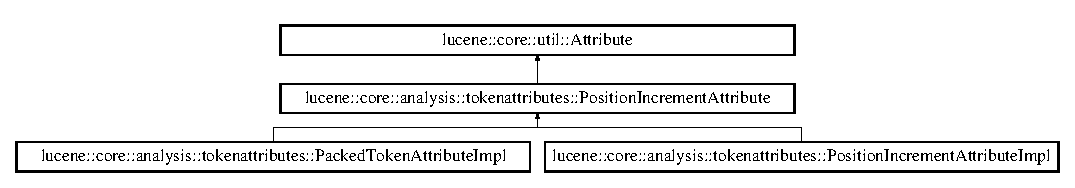
\includegraphics[height=2.084367cm]{classlucene_1_1core_1_1analysis_1_1tokenattributes_1_1PositionIncrementAttribute}
\end{center}
\end{figure}
\subsection*{Public Member Functions}
\begin{DoxyCompactItemize}
\item 
virtual \mbox{\hyperlink{classlucene_1_1core_1_1analysis_1_1tokenattributes_1_1PositionIncrementAttribute_ab97d9e510cff6c1014c283a59aac531c}{$\sim$\+Position\+Increment\+Attribute}} ()
\item 
virtual void \mbox{\hyperlink{classlucene_1_1core_1_1analysis_1_1tokenattributes_1_1PositionIncrementAttribute_a7d012852b01e0b16da72a911a90266b7}{Set\+Position\+Increment}} (const uint32\+\_\+t position\+\_\+increment)=0
\item 
virtual uint32\+\_\+t \mbox{\hyperlink{classlucene_1_1core_1_1analysis_1_1tokenattributes_1_1PositionIncrementAttribute_af0c59c3fbf138881647e46f05468eb13}{Get\+Position\+Increment}} ()=0
\end{DoxyCompactItemize}
\subsection*{Additional Inherited Members}


\subsection{Constructor \& Destructor Documentation}
\mbox{\Hypertarget{classlucene_1_1core_1_1analysis_1_1tokenattributes_1_1PositionIncrementAttribute_ab97d9e510cff6c1014c283a59aac531c}\label{classlucene_1_1core_1_1analysis_1_1tokenattributes_1_1PositionIncrementAttribute_ab97d9e510cff6c1014c283a59aac531c}} 
\index{lucene\+::core\+::analysis\+::tokenattributes\+::\+Position\+Increment\+Attribute@{lucene\+::core\+::analysis\+::tokenattributes\+::\+Position\+Increment\+Attribute}!````~Position\+Increment\+Attribute@{$\sim$\+Position\+Increment\+Attribute}}
\index{````~Position\+Increment\+Attribute@{$\sim$\+Position\+Increment\+Attribute}!lucene\+::core\+::analysis\+::tokenattributes\+::\+Position\+Increment\+Attribute@{lucene\+::core\+::analysis\+::tokenattributes\+::\+Position\+Increment\+Attribute}}
\subsubsection{\texorpdfstring{$\sim$\+Position\+Increment\+Attribute()}{~PositionIncrementAttribute()}}
{\footnotesize\ttfamily virtual lucene\+::core\+::analysis\+::tokenattributes\+::\+Position\+Increment\+Attribute\+::$\sim$\+Position\+Increment\+Attribute (\begin{DoxyParamCaption}{ }\end{DoxyParamCaption})\hspace{0.3cm}{\ttfamily [inline]}, {\ttfamily [virtual]}}



\subsection{Member Function Documentation}
\mbox{\Hypertarget{classlucene_1_1core_1_1analysis_1_1tokenattributes_1_1PositionIncrementAttribute_af0c59c3fbf138881647e46f05468eb13}\label{classlucene_1_1core_1_1analysis_1_1tokenattributes_1_1PositionIncrementAttribute_af0c59c3fbf138881647e46f05468eb13}} 
\index{lucene\+::core\+::analysis\+::tokenattributes\+::\+Position\+Increment\+Attribute@{lucene\+::core\+::analysis\+::tokenattributes\+::\+Position\+Increment\+Attribute}!Get\+Position\+Increment@{Get\+Position\+Increment}}
\index{Get\+Position\+Increment@{Get\+Position\+Increment}!lucene\+::core\+::analysis\+::tokenattributes\+::\+Position\+Increment\+Attribute@{lucene\+::core\+::analysis\+::tokenattributes\+::\+Position\+Increment\+Attribute}}
\subsubsection{\texorpdfstring{Get\+Position\+Increment()}{GetPositionIncrement()}}
{\footnotesize\ttfamily virtual uint32\+\_\+t lucene\+::core\+::analysis\+::tokenattributes\+::\+Position\+Increment\+Attribute\+::\+Get\+Position\+Increment (\begin{DoxyParamCaption}{ }\end{DoxyParamCaption})\hspace{0.3cm}{\ttfamily [pure virtual]}}



Implemented in \mbox{\hyperlink{classlucene_1_1core_1_1analysis_1_1tokenattributes_1_1PositionIncrementAttributeImpl_aed9c6939240be709472fff07ea8f7059}{lucene\+::core\+::analysis\+::tokenattributes\+::\+Position\+Increment\+Attribute\+Impl}}, and \mbox{\hyperlink{classlucene_1_1core_1_1analysis_1_1tokenattributes_1_1PackedTokenAttributeImpl_aeeb6d5e17fb510c402e36d50e39bb9fb}{lucene\+::core\+::analysis\+::tokenattributes\+::\+Packed\+Token\+Attribute\+Impl}}.

\mbox{\Hypertarget{classlucene_1_1core_1_1analysis_1_1tokenattributes_1_1PositionIncrementAttribute_a7d012852b01e0b16da72a911a90266b7}\label{classlucene_1_1core_1_1analysis_1_1tokenattributes_1_1PositionIncrementAttribute_a7d012852b01e0b16da72a911a90266b7}} 
\index{lucene\+::core\+::analysis\+::tokenattributes\+::\+Position\+Increment\+Attribute@{lucene\+::core\+::analysis\+::tokenattributes\+::\+Position\+Increment\+Attribute}!Set\+Position\+Increment@{Set\+Position\+Increment}}
\index{Set\+Position\+Increment@{Set\+Position\+Increment}!lucene\+::core\+::analysis\+::tokenattributes\+::\+Position\+Increment\+Attribute@{lucene\+::core\+::analysis\+::tokenattributes\+::\+Position\+Increment\+Attribute}}
\subsubsection{\texorpdfstring{Set\+Position\+Increment()}{SetPositionIncrement()}}
{\footnotesize\ttfamily virtual void lucene\+::core\+::analysis\+::tokenattributes\+::\+Position\+Increment\+Attribute\+::\+Set\+Position\+Increment (\begin{DoxyParamCaption}\item[{const uint32\+\_\+t}]{position\+\_\+increment }\end{DoxyParamCaption})\hspace{0.3cm}{\ttfamily [pure virtual]}}



Implemented in \mbox{\hyperlink{classlucene_1_1core_1_1analysis_1_1tokenattributes_1_1PositionIncrementAttributeImpl_a7e1d05c2dab9f80a43df0def33f71c27}{lucene\+::core\+::analysis\+::tokenattributes\+::\+Position\+Increment\+Attribute\+Impl}}, and \mbox{\hyperlink{classlucene_1_1core_1_1analysis_1_1tokenattributes_1_1PackedTokenAttributeImpl_a657933594f71883a7271bca05363bc2a}{lucene\+::core\+::analysis\+::tokenattributes\+::\+Packed\+Token\+Attribute\+Impl}}.



The documentation for this class was generated from the following file\+:\begin{DoxyCompactItemize}
\item 
Analysis/\mbox{\hyperlink{Analysis_2Attribute_8h}{Attribute.\+h}}\end{DoxyCompactItemize}

\hypertarget{classlucene_1_1core_1_1analysis_1_1tokenattributes_1_1PositionIncrementAttributeImpl}{}\section{lucene\+:\+:core\+:\+:analysis\+:\+:tokenattributes\+:\+:Position\+Increment\+Attribute\+Impl Class Reference}
\label{classlucene_1_1core_1_1analysis_1_1tokenattributes_1_1PositionIncrementAttributeImpl}\index{lucene\+::core\+::analysis\+::tokenattributes\+::\+Position\+Increment\+Attribute\+Impl@{lucene\+::core\+::analysis\+::tokenattributes\+::\+Position\+Increment\+Attribute\+Impl}}


{\ttfamily \#include $<$Attribute\+Impl.\+h$>$}

Inheritance diagram for lucene\+:\+:core\+:\+:analysis\+:\+:tokenattributes\+:\+:Position\+Increment\+Attribute\+Impl\+:\begin{figure}[H]
\begin{center}
\leavevmode
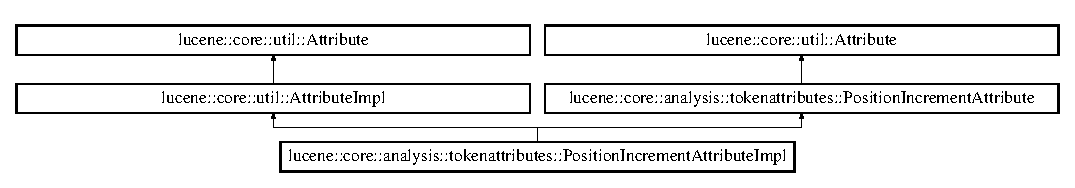
\includegraphics[height=2.084367cm]{classlucene_1_1core_1_1analysis_1_1tokenattributes_1_1PositionIncrementAttributeImpl}
\end{center}
\end{figure}
\subsection*{Public Member Functions}
\begin{DoxyCompactItemize}
\item 
\mbox{\hyperlink{classlucene_1_1core_1_1analysis_1_1tokenattributes_1_1PositionIncrementAttributeImpl_a3a4d29b631b20b0826e06515a76c7a57}{Position\+Increment\+Attribute\+Impl}} ()
\item 
\mbox{\hyperlink{classlucene_1_1core_1_1analysis_1_1tokenattributes_1_1PositionIncrementAttributeImpl_a1982fd1c9538ad47213965386e7d7566}{Position\+Increment\+Attribute\+Impl}} (\mbox{\hyperlink{ZlibCrc32_8h_a2c212835823e3c54a8ab6d95c652660e}{const}} \mbox{\hyperlink{classlucene_1_1core_1_1analysis_1_1tokenattributes_1_1PositionIncrementAttributeImpl}{Position\+Increment\+Attribute\+Impl}} \&other)
\item 
virtual \mbox{\hyperlink{classlucene_1_1core_1_1analysis_1_1tokenattributes_1_1PositionIncrementAttributeImpl_a7a7ac9ea7c224e4f2a62e4b199cddde9}{$\sim$\+Position\+Increment\+Attribute\+Impl}} ()
\item 
void \mbox{\hyperlink{classlucene_1_1core_1_1analysis_1_1tokenattributes_1_1PositionIncrementAttributeImpl_a7e1d05c2dab9f80a43df0def33f71c27}{Set\+Position\+Increment}} (\mbox{\hyperlink{ZlibCrc32_8h_a2c212835823e3c54a8ab6d95c652660e}{const}} uint32\+\_\+t \mbox{\hyperlink{classlucene_1_1core_1_1analysis_1_1tokenattributes_1_1PositionIncrementAttributeImpl_a3de757124d0bf5a9395e8c943c4ee5cf}{position\+\_\+increment}}) override
\item 
uint32\+\_\+t \mbox{\hyperlink{classlucene_1_1core_1_1analysis_1_1tokenattributes_1_1PositionIncrementAttributeImpl_aed9c6939240be709472fff07ea8f7059}{Get\+Position\+Increment}} () override
\item 
void \mbox{\hyperlink{classlucene_1_1core_1_1analysis_1_1tokenattributes_1_1PositionIncrementAttributeImpl_a2ede3f15304f9760ad60009335123ece}{Reflect\+With}} (\mbox{\hyperlink{namespacelucene_1_1core_1_1util_a7dbb701adaed055f73fb95eec83da10a}{lucene\+::core\+::util\+::\+Attribute\+Reflector}} \&reflector) override
\item 
void \mbox{\hyperlink{classlucene_1_1core_1_1analysis_1_1tokenattributes_1_1PositionIncrementAttributeImpl_adb934ddcbf6f584c50a72c0980b88761}{End}} () override
\item 
void \mbox{\hyperlink{classlucene_1_1core_1_1analysis_1_1tokenattributes_1_1PositionIncrementAttributeImpl_a49cd1a34361a145c3b674f1f3d529641}{Clear}} () override
\item 
bool \mbox{\hyperlink{classlucene_1_1core_1_1analysis_1_1tokenattributes_1_1PositionIncrementAttributeImpl_a5450f58da2745c914e68e7a650e78cc3}{operator==}} (\mbox{\hyperlink{ZlibCrc32_8h_a2c212835823e3c54a8ab6d95c652660e}{const}} \mbox{\hyperlink{classlucene_1_1core_1_1analysis_1_1tokenattributes_1_1PositionIncrementAttributeImpl}{Position\+Increment\+Attribute\+Impl}} \&other) \mbox{\hyperlink{ZlibCrc32_8h_a2c212835823e3c54a8ab6d95c652660e}{const}}
\item 
std\+::vector$<$ std\+::type\+\_\+index $>$ \mbox{\hyperlink{classlucene_1_1core_1_1analysis_1_1tokenattributes_1_1PositionIncrementAttributeImpl_ab6028133ca375bdcb9774650828e7388}{Attributes}} () override
\item 
void \mbox{\hyperlink{classlucene_1_1core_1_1analysis_1_1tokenattributes_1_1PositionIncrementAttributeImpl_a887e391d3db93f6a8e76b6b464d60547}{Shallow\+Copy\+To}} (\mbox{\hyperlink{classlucene_1_1core_1_1util_1_1AttributeImpl}{lucene\+::core\+::util\+::\+Attribute\+Impl}} \&attr\+\_\+impl) override
\item 
\mbox{\hyperlink{classlucene_1_1core_1_1analysis_1_1tokenattributes_1_1PositionIncrementAttributeImpl}{Position\+Increment\+Attribute\+Impl}} \& \mbox{\hyperlink{classlucene_1_1core_1_1analysis_1_1tokenattributes_1_1PositionIncrementAttributeImpl_a8fccb463e29cc9cb90e7689cc7161488}{operator=}} (\mbox{\hyperlink{ZlibCrc32_8h_a2c212835823e3c54a8ab6d95c652660e}{const}} \mbox{\hyperlink{classlucene_1_1core_1_1util_1_1AttributeImpl}{lucene\+::core\+::util\+::\+Attribute\+Impl}} \&other)
\item 
\mbox{\hyperlink{classlucene_1_1core_1_1analysis_1_1tokenattributes_1_1PositionIncrementAttributeImpl}{Position\+Increment\+Attribute\+Impl}} \& \mbox{\hyperlink{classlucene_1_1core_1_1analysis_1_1tokenattributes_1_1PositionIncrementAttributeImpl_a89b28d766574af0ba1e521adf811fe71}{operator=}} (\mbox{\hyperlink{ZlibCrc32_8h_a2c212835823e3c54a8ab6d95c652660e}{const}} \mbox{\hyperlink{classlucene_1_1core_1_1analysis_1_1tokenattributes_1_1PositionIncrementAttributeImpl}{Position\+Increment\+Attribute\+Impl}} \&other)
\item 
\mbox{\hyperlink{classlucene_1_1core_1_1util_1_1AttributeImpl}{lucene\+::core\+::util\+::\+Attribute\+Impl}} $\ast$ \mbox{\hyperlink{classlucene_1_1core_1_1analysis_1_1tokenattributes_1_1PositionIncrementAttributeImpl_a68907cad12693754f1286678a7c78c21}{Clone}} () override
\end{DoxyCompactItemize}
\subsection*{Private Attributes}
\begin{DoxyCompactItemize}
\item 
uint32\+\_\+t \mbox{\hyperlink{classlucene_1_1core_1_1analysis_1_1tokenattributes_1_1PositionIncrementAttributeImpl_a3de757124d0bf5a9395e8c943c4ee5cf}{position\+\_\+increment}}
\end{DoxyCompactItemize}
\subsection*{Additional Inherited Members}


\subsection{Constructor \& Destructor Documentation}
\mbox{\Hypertarget{classlucene_1_1core_1_1analysis_1_1tokenattributes_1_1PositionIncrementAttributeImpl_a3a4d29b631b20b0826e06515a76c7a57}\label{classlucene_1_1core_1_1analysis_1_1tokenattributes_1_1PositionIncrementAttributeImpl_a3a4d29b631b20b0826e06515a76c7a57}} 
\index{lucene\+::core\+::analysis\+::tokenattributes\+::\+Position\+Increment\+Attribute\+Impl@{lucene\+::core\+::analysis\+::tokenattributes\+::\+Position\+Increment\+Attribute\+Impl}!Position\+Increment\+Attribute\+Impl@{Position\+Increment\+Attribute\+Impl}}
\index{Position\+Increment\+Attribute\+Impl@{Position\+Increment\+Attribute\+Impl}!lucene\+::core\+::analysis\+::tokenattributes\+::\+Position\+Increment\+Attribute\+Impl@{lucene\+::core\+::analysis\+::tokenattributes\+::\+Position\+Increment\+Attribute\+Impl}}
\subsubsection{\texorpdfstring{Position\+Increment\+Attribute\+Impl()}{PositionIncrementAttributeImpl()}\hspace{0.1cm}{\footnotesize\ttfamily [1/2]}}
{\footnotesize\ttfamily Position\+Increment\+Attribute\+Impl\+::\+Position\+Increment\+Attribute\+Impl (\begin{DoxyParamCaption}{ }\end{DoxyParamCaption})}

\mbox{\hyperlink{classlucene_1_1core_1_1analysis_1_1tokenattributes_1_1PositionIncrementAttributeImpl}{Position\+Increment\+Attribute\+Impl}} \mbox{\Hypertarget{classlucene_1_1core_1_1analysis_1_1tokenattributes_1_1PositionIncrementAttributeImpl_a1982fd1c9538ad47213965386e7d7566}\label{classlucene_1_1core_1_1analysis_1_1tokenattributes_1_1PositionIncrementAttributeImpl_a1982fd1c9538ad47213965386e7d7566}} 
\index{lucene\+::core\+::analysis\+::tokenattributes\+::\+Position\+Increment\+Attribute\+Impl@{lucene\+::core\+::analysis\+::tokenattributes\+::\+Position\+Increment\+Attribute\+Impl}!Position\+Increment\+Attribute\+Impl@{Position\+Increment\+Attribute\+Impl}}
\index{Position\+Increment\+Attribute\+Impl@{Position\+Increment\+Attribute\+Impl}!lucene\+::core\+::analysis\+::tokenattributes\+::\+Position\+Increment\+Attribute\+Impl@{lucene\+::core\+::analysis\+::tokenattributes\+::\+Position\+Increment\+Attribute\+Impl}}
\subsubsection{\texorpdfstring{Position\+Increment\+Attribute\+Impl()}{PositionIncrementAttributeImpl()}\hspace{0.1cm}{\footnotesize\ttfamily [2/2]}}
{\footnotesize\ttfamily Position\+Increment\+Attribute\+Impl\+::\+Position\+Increment\+Attribute\+Impl (\begin{DoxyParamCaption}\item[{\mbox{\hyperlink{ZlibCrc32_8h_a2c212835823e3c54a8ab6d95c652660e}{const}} \mbox{\hyperlink{classlucene_1_1core_1_1analysis_1_1tokenattributes_1_1PositionIncrementAttributeImpl}{Position\+Increment\+Attribute\+Impl}} \&}]{other }\end{DoxyParamCaption})}

\mbox{\Hypertarget{classlucene_1_1core_1_1analysis_1_1tokenattributes_1_1PositionIncrementAttributeImpl_a7a7ac9ea7c224e4f2a62e4b199cddde9}\label{classlucene_1_1core_1_1analysis_1_1tokenattributes_1_1PositionIncrementAttributeImpl_a7a7ac9ea7c224e4f2a62e4b199cddde9}} 
\index{lucene\+::core\+::analysis\+::tokenattributes\+::\+Position\+Increment\+Attribute\+Impl@{lucene\+::core\+::analysis\+::tokenattributes\+::\+Position\+Increment\+Attribute\+Impl}!````~Position\+Increment\+Attribute\+Impl@{$\sim$\+Position\+Increment\+Attribute\+Impl}}
\index{````~Position\+Increment\+Attribute\+Impl@{$\sim$\+Position\+Increment\+Attribute\+Impl}!lucene\+::core\+::analysis\+::tokenattributes\+::\+Position\+Increment\+Attribute\+Impl@{lucene\+::core\+::analysis\+::tokenattributes\+::\+Position\+Increment\+Attribute\+Impl}}
\subsubsection{\texorpdfstring{$\sim$\+Position\+Increment\+Attribute\+Impl()}{~PositionIncrementAttributeImpl()}}
{\footnotesize\ttfamily Position\+Increment\+Attribute\+Impl\+::$\sim$\+Position\+Increment\+Attribute\+Impl (\begin{DoxyParamCaption}{ }\end{DoxyParamCaption})\hspace{0.3cm}{\ttfamily [virtual]}}



\subsection{Member Function Documentation}
\mbox{\Hypertarget{classlucene_1_1core_1_1analysis_1_1tokenattributes_1_1PositionIncrementAttributeImpl_ab6028133ca375bdcb9774650828e7388}\label{classlucene_1_1core_1_1analysis_1_1tokenattributes_1_1PositionIncrementAttributeImpl_ab6028133ca375bdcb9774650828e7388}} 
\index{lucene\+::core\+::analysis\+::tokenattributes\+::\+Position\+Increment\+Attribute\+Impl@{lucene\+::core\+::analysis\+::tokenattributes\+::\+Position\+Increment\+Attribute\+Impl}!Attributes@{Attributes}}
\index{Attributes@{Attributes}!lucene\+::core\+::analysis\+::tokenattributes\+::\+Position\+Increment\+Attribute\+Impl@{lucene\+::core\+::analysis\+::tokenattributes\+::\+Position\+Increment\+Attribute\+Impl}}
\subsubsection{\texorpdfstring{Attributes()}{Attributes()}}
{\footnotesize\ttfamily std\+::vector$<$ std\+::type\+\_\+index $>$ Position\+Increment\+Attribute\+Impl\+::\+Attributes (\begin{DoxyParamCaption}{ }\end{DoxyParamCaption})\hspace{0.3cm}{\ttfamily [override]}, {\ttfamily [virtual]}}



Implements \mbox{\hyperlink{classlucene_1_1core_1_1util_1_1AttributeImpl_ac0631e6a7a11044883bc97447716d7cc}{lucene\+::core\+::util\+::\+Attribute\+Impl}}.

\mbox{\Hypertarget{classlucene_1_1core_1_1analysis_1_1tokenattributes_1_1PositionIncrementAttributeImpl_a49cd1a34361a145c3b674f1f3d529641}\label{classlucene_1_1core_1_1analysis_1_1tokenattributes_1_1PositionIncrementAttributeImpl_a49cd1a34361a145c3b674f1f3d529641}} 
\index{lucene\+::core\+::analysis\+::tokenattributes\+::\+Position\+Increment\+Attribute\+Impl@{lucene\+::core\+::analysis\+::tokenattributes\+::\+Position\+Increment\+Attribute\+Impl}!Clear@{Clear}}
\index{Clear@{Clear}!lucene\+::core\+::analysis\+::tokenattributes\+::\+Position\+Increment\+Attribute\+Impl@{lucene\+::core\+::analysis\+::tokenattributes\+::\+Position\+Increment\+Attribute\+Impl}}
\subsubsection{\texorpdfstring{Clear()}{Clear()}}
{\footnotesize\ttfamily void Position\+Increment\+Attribute\+Impl\+::\+Clear (\begin{DoxyParamCaption}{ }\end{DoxyParamCaption})\hspace{0.3cm}{\ttfamily [override]}, {\ttfamily [virtual]}}



Implements \mbox{\hyperlink{classlucene_1_1core_1_1util_1_1AttributeImpl_a04897a00a902f7a345dd44bbc4b482a8}{lucene\+::core\+::util\+::\+Attribute\+Impl}}.

\mbox{\Hypertarget{classlucene_1_1core_1_1analysis_1_1tokenattributes_1_1PositionIncrementAttributeImpl_a68907cad12693754f1286678a7c78c21}\label{classlucene_1_1core_1_1analysis_1_1tokenattributes_1_1PositionIncrementAttributeImpl_a68907cad12693754f1286678a7c78c21}} 
\index{lucene\+::core\+::analysis\+::tokenattributes\+::\+Position\+Increment\+Attribute\+Impl@{lucene\+::core\+::analysis\+::tokenattributes\+::\+Position\+Increment\+Attribute\+Impl}!Clone@{Clone}}
\index{Clone@{Clone}!lucene\+::core\+::analysis\+::tokenattributes\+::\+Position\+Increment\+Attribute\+Impl@{lucene\+::core\+::analysis\+::tokenattributes\+::\+Position\+Increment\+Attribute\+Impl}}
\subsubsection{\texorpdfstring{Clone()}{Clone()}}
{\footnotesize\ttfamily \mbox{\hyperlink{classlucene_1_1core_1_1util_1_1AttributeImpl}{Attribute\+Impl}} $\ast$ Position\+Increment\+Attribute\+Impl\+::\+Clone (\begin{DoxyParamCaption}{ }\end{DoxyParamCaption})\hspace{0.3cm}{\ttfamily [override]}, {\ttfamily [virtual]}}



Implements \mbox{\hyperlink{classlucene_1_1core_1_1util_1_1AttributeImpl_a135318ad4c7c17b3d85e625e32fb42cd}{lucene\+::core\+::util\+::\+Attribute\+Impl}}.

\mbox{\Hypertarget{classlucene_1_1core_1_1analysis_1_1tokenattributes_1_1PositionIncrementAttributeImpl_adb934ddcbf6f584c50a72c0980b88761}\label{classlucene_1_1core_1_1analysis_1_1tokenattributes_1_1PositionIncrementAttributeImpl_adb934ddcbf6f584c50a72c0980b88761}} 
\index{lucene\+::core\+::analysis\+::tokenattributes\+::\+Position\+Increment\+Attribute\+Impl@{lucene\+::core\+::analysis\+::tokenattributes\+::\+Position\+Increment\+Attribute\+Impl}!End@{End}}
\index{End@{End}!lucene\+::core\+::analysis\+::tokenattributes\+::\+Position\+Increment\+Attribute\+Impl@{lucene\+::core\+::analysis\+::tokenattributes\+::\+Position\+Increment\+Attribute\+Impl}}
\subsubsection{\texorpdfstring{End()}{End()}}
{\footnotesize\ttfamily void Position\+Increment\+Attribute\+Impl\+::\+End (\begin{DoxyParamCaption}{ }\end{DoxyParamCaption})\hspace{0.3cm}{\ttfamily [override]}, {\ttfamily [virtual]}}

Attribute\+Impl 

Reimplemented from \mbox{\hyperlink{classlucene_1_1core_1_1util_1_1AttributeImpl_a9a662ddc9b72bc9711883a25b8379ea9}{lucene\+::core\+::util\+::\+Attribute\+Impl}}.

\mbox{\Hypertarget{classlucene_1_1core_1_1analysis_1_1tokenattributes_1_1PositionIncrementAttributeImpl_aed9c6939240be709472fff07ea8f7059}\label{classlucene_1_1core_1_1analysis_1_1tokenattributes_1_1PositionIncrementAttributeImpl_aed9c6939240be709472fff07ea8f7059}} 
\index{lucene\+::core\+::analysis\+::tokenattributes\+::\+Position\+Increment\+Attribute\+Impl@{lucene\+::core\+::analysis\+::tokenattributes\+::\+Position\+Increment\+Attribute\+Impl}!Get\+Position\+Increment@{Get\+Position\+Increment}}
\index{Get\+Position\+Increment@{Get\+Position\+Increment}!lucene\+::core\+::analysis\+::tokenattributes\+::\+Position\+Increment\+Attribute\+Impl@{lucene\+::core\+::analysis\+::tokenattributes\+::\+Position\+Increment\+Attribute\+Impl}}
\subsubsection{\texorpdfstring{Get\+Position\+Increment()}{GetPositionIncrement()}}
{\footnotesize\ttfamily uint32\+\_\+t Position\+Increment\+Attribute\+Impl\+::\+Get\+Position\+Increment (\begin{DoxyParamCaption}{ }\end{DoxyParamCaption})\hspace{0.3cm}{\ttfamily [override]}, {\ttfamily [virtual]}}



Implements \mbox{\hyperlink{classlucene_1_1core_1_1analysis_1_1tokenattributes_1_1PositionIncrementAttribute_af0c59c3fbf138881647e46f05468eb13}{lucene\+::core\+::analysis\+::tokenattributes\+::\+Position\+Increment\+Attribute}}.

\mbox{\Hypertarget{classlucene_1_1core_1_1analysis_1_1tokenattributes_1_1PositionIncrementAttributeImpl_a8fccb463e29cc9cb90e7689cc7161488}\label{classlucene_1_1core_1_1analysis_1_1tokenattributes_1_1PositionIncrementAttributeImpl_a8fccb463e29cc9cb90e7689cc7161488}} 
\index{lucene\+::core\+::analysis\+::tokenattributes\+::\+Position\+Increment\+Attribute\+Impl@{lucene\+::core\+::analysis\+::tokenattributes\+::\+Position\+Increment\+Attribute\+Impl}!operator=@{operator=}}
\index{operator=@{operator=}!lucene\+::core\+::analysis\+::tokenattributes\+::\+Position\+Increment\+Attribute\+Impl@{lucene\+::core\+::analysis\+::tokenattributes\+::\+Position\+Increment\+Attribute\+Impl}}
\subsubsection{\texorpdfstring{operator=()}{operator=()}\hspace{0.1cm}{\footnotesize\ttfamily [1/2]}}
{\footnotesize\ttfamily \mbox{\hyperlink{classlucene_1_1core_1_1analysis_1_1tokenattributes_1_1PositionIncrementAttributeImpl}{Position\+Increment\+Attribute\+Impl}} \& Position\+Increment\+Attribute\+Impl\+::operator= (\begin{DoxyParamCaption}\item[{\mbox{\hyperlink{ZlibCrc32_8h_a2c212835823e3c54a8ab6d95c652660e}{const}} \mbox{\hyperlink{classlucene_1_1core_1_1util_1_1AttributeImpl}{lucene\+::core\+::util\+::\+Attribute\+Impl}} \&}]{other }\end{DoxyParamCaption})\hspace{0.3cm}{\ttfamily [virtual]}}



Implements \mbox{\hyperlink{classlucene_1_1core_1_1util_1_1AttributeImpl_ab032e399d03ce2f58c76881cf2b92325}{lucene\+::core\+::util\+::\+Attribute\+Impl}}.

\mbox{\Hypertarget{classlucene_1_1core_1_1analysis_1_1tokenattributes_1_1PositionIncrementAttributeImpl_a89b28d766574af0ba1e521adf811fe71}\label{classlucene_1_1core_1_1analysis_1_1tokenattributes_1_1PositionIncrementAttributeImpl_a89b28d766574af0ba1e521adf811fe71}} 
\index{lucene\+::core\+::analysis\+::tokenattributes\+::\+Position\+Increment\+Attribute\+Impl@{lucene\+::core\+::analysis\+::tokenattributes\+::\+Position\+Increment\+Attribute\+Impl}!operator=@{operator=}}
\index{operator=@{operator=}!lucene\+::core\+::analysis\+::tokenattributes\+::\+Position\+Increment\+Attribute\+Impl@{lucene\+::core\+::analysis\+::tokenattributes\+::\+Position\+Increment\+Attribute\+Impl}}
\subsubsection{\texorpdfstring{operator=()}{operator=()}\hspace{0.1cm}{\footnotesize\ttfamily [2/2]}}
{\footnotesize\ttfamily \mbox{\hyperlink{classlucene_1_1core_1_1analysis_1_1tokenattributes_1_1PositionIncrementAttributeImpl}{Position\+Increment\+Attribute\+Impl}} \& Position\+Increment\+Attribute\+Impl\+::operator= (\begin{DoxyParamCaption}\item[{\mbox{\hyperlink{ZlibCrc32_8h_a2c212835823e3c54a8ab6d95c652660e}{const}} \mbox{\hyperlink{classlucene_1_1core_1_1analysis_1_1tokenattributes_1_1PositionIncrementAttributeImpl}{Position\+Increment\+Attribute\+Impl}} \&}]{other }\end{DoxyParamCaption})}

\mbox{\Hypertarget{classlucene_1_1core_1_1analysis_1_1tokenattributes_1_1PositionIncrementAttributeImpl_a5450f58da2745c914e68e7a650e78cc3}\label{classlucene_1_1core_1_1analysis_1_1tokenattributes_1_1PositionIncrementAttributeImpl_a5450f58da2745c914e68e7a650e78cc3}} 
\index{lucene\+::core\+::analysis\+::tokenattributes\+::\+Position\+Increment\+Attribute\+Impl@{lucene\+::core\+::analysis\+::tokenattributes\+::\+Position\+Increment\+Attribute\+Impl}!operator==@{operator==}}
\index{operator==@{operator==}!lucene\+::core\+::analysis\+::tokenattributes\+::\+Position\+Increment\+Attribute\+Impl@{lucene\+::core\+::analysis\+::tokenattributes\+::\+Position\+Increment\+Attribute\+Impl}}
\subsubsection{\texorpdfstring{operator==()}{operator==()}}
{\footnotesize\ttfamily bool Position\+Increment\+Attribute\+Impl\+::operator== (\begin{DoxyParamCaption}\item[{\mbox{\hyperlink{ZlibCrc32_8h_a2c212835823e3c54a8ab6d95c652660e}{const}} \mbox{\hyperlink{classlucene_1_1core_1_1analysis_1_1tokenattributes_1_1PositionIncrementAttributeImpl}{Position\+Increment\+Attribute\+Impl}} \&}]{other }\end{DoxyParamCaption}) const}

\mbox{\Hypertarget{classlucene_1_1core_1_1analysis_1_1tokenattributes_1_1PositionIncrementAttributeImpl_a2ede3f15304f9760ad60009335123ece}\label{classlucene_1_1core_1_1analysis_1_1tokenattributes_1_1PositionIncrementAttributeImpl_a2ede3f15304f9760ad60009335123ece}} 
\index{lucene\+::core\+::analysis\+::tokenattributes\+::\+Position\+Increment\+Attribute\+Impl@{lucene\+::core\+::analysis\+::tokenattributes\+::\+Position\+Increment\+Attribute\+Impl}!Reflect\+With@{Reflect\+With}}
\index{Reflect\+With@{Reflect\+With}!lucene\+::core\+::analysis\+::tokenattributes\+::\+Position\+Increment\+Attribute\+Impl@{lucene\+::core\+::analysis\+::tokenattributes\+::\+Position\+Increment\+Attribute\+Impl}}
\subsubsection{\texorpdfstring{Reflect\+With()}{ReflectWith()}}
{\footnotesize\ttfamily void Position\+Increment\+Attribute\+Impl\+::\+Reflect\+With (\begin{DoxyParamCaption}\item[{\mbox{\hyperlink{namespacelucene_1_1core_1_1util_a7dbb701adaed055f73fb95eec83da10a}{lucene\+::core\+::util\+::\+Attribute\+Reflector}} \&}]{reflector }\end{DoxyParamCaption})\hspace{0.3cm}{\ttfamily [override]}, {\ttfamily [virtual]}}



Implements \mbox{\hyperlink{classlucene_1_1core_1_1util_1_1AttributeImpl_a84d34275fb1ed67ac36fad7ff6388096}{lucene\+::core\+::util\+::\+Attribute\+Impl}}.

\mbox{\Hypertarget{classlucene_1_1core_1_1analysis_1_1tokenattributes_1_1PositionIncrementAttributeImpl_a7e1d05c2dab9f80a43df0def33f71c27}\label{classlucene_1_1core_1_1analysis_1_1tokenattributes_1_1PositionIncrementAttributeImpl_a7e1d05c2dab9f80a43df0def33f71c27}} 
\index{lucene\+::core\+::analysis\+::tokenattributes\+::\+Position\+Increment\+Attribute\+Impl@{lucene\+::core\+::analysis\+::tokenattributes\+::\+Position\+Increment\+Attribute\+Impl}!Set\+Position\+Increment@{Set\+Position\+Increment}}
\index{Set\+Position\+Increment@{Set\+Position\+Increment}!lucene\+::core\+::analysis\+::tokenattributes\+::\+Position\+Increment\+Attribute\+Impl@{lucene\+::core\+::analysis\+::tokenattributes\+::\+Position\+Increment\+Attribute\+Impl}}
\subsubsection{\texorpdfstring{Set\+Position\+Increment()}{SetPositionIncrement()}}
{\footnotesize\ttfamily void Position\+Increment\+Attribute\+Impl\+::\+Set\+Position\+Increment (\begin{DoxyParamCaption}\item[{\mbox{\hyperlink{ZlibCrc32_8h_a2c212835823e3c54a8ab6d95c652660e}{const}} uint32\+\_\+t}]{position\+\_\+increment }\end{DoxyParamCaption})\hspace{0.3cm}{\ttfamily [override]}, {\ttfamily [virtual]}}



Implements \mbox{\hyperlink{classlucene_1_1core_1_1analysis_1_1tokenattributes_1_1PositionIncrementAttribute_a7d012852b01e0b16da72a911a90266b7}{lucene\+::core\+::analysis\+::tokenattributes\+::\+Position\+Increment\+Attribute}}.

\mbox{\Hypertarget{classlucene_1_1core_1_1analysis_1_1tokenattributes_1_1PositionIncrementAttributeImpl_a887e391d3db93f6a8e76b6b464d60547}\label{classlucene_1_1core_1_1analysis_1_1tokenattributes_1_1PositionIncrementAttributeImpl_a887e391d3db93f6a8e76b6b464d60547}} 
\index{lucene\+::core\+::analysis\+::tokenattributes\+::\+Position\+Increment\+Attribute\+Impl@{lucene\+::core\+::analysis\+::tokenattributes\+::\+Position\+Increment\+Attribute\+Impl}!Shallow\+Copy\+To@{Shallow\+Copy\+To}}
\index{Shallow\+Copy\+To@{Shallow\+Copy\+To}!lucene\+::core\+::analysis\+::tokenattributes\+::\+Position\+Increment\+Attribute\+Impl@{lucene\+::core\+::analysis\+::tokenattributes\+::\+Position\+Increment\+Attribute\+Impl}}
\subsubsection{\texorpdfstring{Shallow\+Copy\+To()}{ShallowCopyTo()}}
{\footnotesize\ttfamily void Position\+Increment\+Attribute\+Impl\+::\+Shallow\+Copy\+To (\begin{DoxyParamCaption}\item[{\mbox{\hyperlink{classlucene_1_1core_1_1util_1_1AttributeImpl}{lucene\+::core\+::util\+::\+Attribute\+Impl}} \&}]{attr\+\_\+impl }\end{DoxyParamCaption})\hspace{0.3cm}{\ttfamily [override]}, {\ttfamily [virtual]}}



Implements \mbox{\hyperlink{classlucene_1_1core_1_1util_1_1AttributeImpl_a010e8937832f53139c8fe42757476895}{lucene\+::core\+::util\+::\+Attribute\+Impl}}.



\subsection{Member Data Documentation}
\mbox{\Hypertarget{classlucene_1_1core_1_1analysis_1_1tokenattributes_1_1PositionIncrementAttributeImpl_a3de757124d0bf5a9395e8c943c4ee5cf}\label{classlucene_1_1core_1_1analysis_1_1tokenattributes_1_1PositionIncrementAttributeImpl_a3de757124d0bf5a9395e8c943c4ee5cf}} 
\index{lucene\+::core\+::analysis\+::tokenattributes\+::\+Position\+Increment\+Attribute\+Impl@{lucene\+::core\+::analysis\+::tokenattributes\+::\+Position\+Increment\+Attribute\+Impl}!position\+\_\+increment@{position\+\_\+increment}}
\index{position\+\_\+increment@{position\+\_\+increment}!lucene\+::core\+::analysis\+::tokenattributes\+::\+Position\+Increment\+Attribute\+Impl@{lucene\+::core\+::analysis\+::tokenattributes\+::\+Position\+Increment\+Attribute\+Impl}}
\subsubsection{\texorpdfstring{position\+\_\+increment}{position\_increment}}
{\footnotesize\ttfamily uint32\+\_\+t lucene\+::core\+::analysis\+::tokenattributes\+::\+Position\+Increment\+Attribute\+Impl\+::position\+\_\+increment\hspace{0.3cm}{\ttfamily [private]}}



The documentation for this class was generated from the following files\+:\begin{DoxyCompactItemize}
\item 
Analysis/\mbox{\hyperlink{AttributeImpl_8h}{Attribute\+Impl.\+h}}\item 
Analysis/\mbox{\hyperlink{AttributeImpl_8cpp}{Attribute\+Impl.\+cpp}}\end{DoxyCompactItemize}

\hypertarget{classlucene_1_1core_1_1analysis_1_1tokenattributes_1_1PositionLengthAttribute}{}\section{lucene\+:\+:core\+:\+:analysis\+:\+:tokenattributes\+:\+:Position\+Length\+Attribute Class Reference}
\label{classlucene_1_1core_1_1analysis_1_1tokenattributes_1_1PositionLengthAttribute}\index{lucene\+::core\+::analysis\+::tokenattributes\+::\+Position\+Length\+Attribute@{lucene\+::core\+::analysis\+::tokenattributes\+::\+Position\+Length\+Attribute}}


{\ttfamily \#include $<$Attribute.\+h$>$}

Inheritance diagram for lucene\+:\+:core\+:\+:analysis\+:\+:tokenattributes\+:\+:Position\+Length\+Attribute\+:\begin{figure}[H]
\begin{center}
\leavevmode
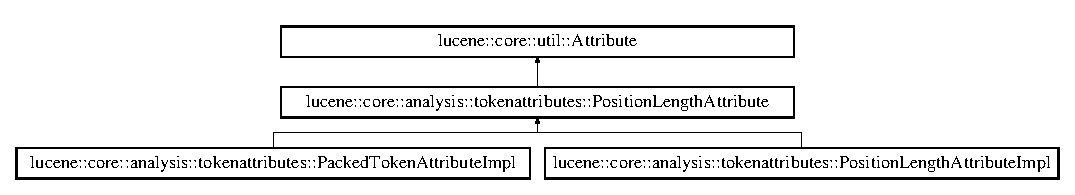
\includegraphics[height=2.176166cm]{classlucene_1_1core_1_1analysis_1_1tokenattributes_1_1PositionLengthAttribute}
\end{center}
\end{figure}
\subsection*{Public Member Functions}
\begin{DoxyCompactItemize}
\item 
virtual \mbox{\hyperlink{classlucene_1_1core_1_1analysis_1_1tokenattributes_1_1PositionLengthAttribute_a1a1260d8ec8ea8d25dda405698268d3f}{$\sim$\+Position\+Length\+Attribute}} ()
\item 
virtual void \mbox{\hyperlink{classlucene_1_1core_1_1analysis_1_1tokenattributes_1_1PositionLengthAttribute_a514415965bae0dd392cbb8d65ea4d808}{Set\+Position\+Length}} (const uint32\+\_\+t position\+\_\+length)=0
\item 
virtual uint32\+\_\+t \mbox{\hyperlink{classlucene_1_1core_1_1analysis_1_1tokenattributes_1_1PositionLengthAttribute_a6325424899959bb480f161e0d5490bfd}{Get\+Position\+Length}} ()=0
\end{DoxyCompactItemize}
\subsection*{Additional Inherited Members}


\subsection{Constructor \& Destructor Documentation}
\mbox{\Hypertarget{classlucene_1_1core_1_1analysis_1_1tokenattributes_1_1PositionLengthAttribute_a1a1260d8ec8ea8d25dda405698268d3f}\label{classlucene_1_1core_1_1analysis_1_1tokenattributes_1_1PositionLengthAttribute_a1a1260d8ec8ea8d25dda405698268d3f}} 
\index{lucene\+::core\+::analysis\+::tokenattributes\+::\+Position\+Length\+Attribute@{lucene\+::core\+::analysis\+::tokenattributes\+::\+Position\+Length\+Attribute}!````~Position\+Length\+Attribute@{$\sim$\+Position\+Length\+Attribute}}
\index{````~Position\+Length\+Attribute@{$\sim$\+Position\+Length\+Attribute}!lucene\+::core\+::analysis\+::tokenattributes\+::\+Position\+Length\+Attribute@{lucene\+::core\+::analysis\+::tokenattributes\+::\+Position\+Length\+Attribute}}
\subsubsection{\texorpdfstring{$\sim$\+Position\+Length\+Attribute()}{~PositionLengthAttribute()}}
{\footnotesize\ttfamily virtual lucene\+::core\+::analysis\+::tokenattributes\+::\+Position\+Length\+Attribute\+::$\sim$\+Position\+Length\+Attribute (\begin{DoxyParamCaption}{ }\end{DoxyParamCaption})\hspace{0.3cm}{\ttfamily [inline]}, {\ttfamily [virtual]}}



\subsection{Member Function Documentation}
\mbox{\Hypertarget{classlucene_1_1core_1_1analysis_1_1tokenattributes_1_1PositionLengthAttribute_a6325424899959bb480f161e0d5490bfd}\label{classlucene_1_1core_1_1analysis_1_1tokenattributes_1_1PositionLengthAttribute_a6325424899959bb480f161e0d5490bfd}} 
\index{lucene\+::core\+::analysis\+::tokenattributes\+::\+Position\+Length\+Attribute@{lucene\+::core\+::analysis\+::tokenattributes\+::\+Position\+Length\+Attribute}!Get\+Position\+Length@{Get\+Position\+Length}}
\index{Get\+Position\+Length@{Get\+Position\+Length}!lucene\+::core\+::analysis\+::tokenattributes\+::\+Position\+Length\+Attribute@{lucene\+::core\+::analysis\+::tokenattributes\+::\+Position\+Length\+Attribute}}
\subsubsection{\texorpdfstring{Get\+Position\+Length()}{GetPositionLength()}}
{\footnotesize\ttfamily virtual uint32\+\_\+t lucene\+::core\+::analysis\+::tokenattributes\+::\+Position\+Length\+Attribute\+::\+Get\+Position\+Length (\begin{DoxyParamCaption}{ }\end{DoxyParamCaption})\hspace{0.3cm}{\ttfamily [pure virtual]}}



Implemented in \mbox{\hyperlink{classlucene_1_1core_1_1analysis_1_1tokenattributes_1_1PositionLengthAttributeImpl_a79dfa19c547152a263d601dfaf62fe9b}{lucene\+::core\+::analysis\+::tokenattributes\+::\+Position\+Length\+Attribute\+Impl}}, and \mbox{\hyperlink{classlucene_1_1core_1_1analysis_1_1tokenattributes_1_1PackedTokenAttributeImpl_a4b5a93a1d9b61cf1504b382d24c1e6d9}{lucene\+::core\+::analysis\+::tokenattributes\+::\+Packed\+Token\+Attribute\+Impl}}.

\mbox{\Hypertarget{classlucene_1_1core_1_1analysis_1_1tokenattributes_1_1PositionLengthAttribute_a514415965bae0dd392cbb8d65ea4d808}\label{classlucene_1_1core_1_1analysis_1_1tokenattributes_1_1PositionLengthAttribute_a514415965bae0dd392cbb8d65ea4d808}} 
\index{lucene\+::core\+::analysis\+::tokenattributes\+::\+Position\+Length\+Attribute@{lucene\+::core\+::analysis\+::tokenattributes\+::\+Position\+Length\+Attribute}!Set\+Position\+Length@{Set\+Position\+Length}}
\index{Set\+Position\+Length@{Set\+Position\+Length}!lucene\+::core\+::analysis\+::tokenattributes\+::\+Position\+Length\+Attribute@{lucene\+::core\+::analysis\+::tokenattributes\+::\+Position\+Length\+Attribute}}
\subsubsection{\texorpdfstring{Set\+Position\+Length()}{SetPositionLength()}}
{\footnotesize\ttfamily virtual void lucene\+::core\+::analysis\+::tokenattributes\+::\+Position\+Length\+Attribute\+::\+Set\+Position\+Length (\begin{DoxyParamCaption}\item[{const uint32\+\_\+t}]{position\+\_\+length }\end{DoxyParamCaption})\hspace{0.3cm}{\ttfamily [pure virtual]}}



Implemented in \mbox{\hyperlink{classlucene_1_1core_1_1analysis_1_1tokenattributes_1_1PositionLengthAttributeImpl_a8b09235c697cf5157ca4351653fcbaf4}{lucene\+::core\+::analysis\+::tokenattributes\+::\+Position\+Length\+Attribute\+Impl}}, and \mbox{\hyperlink{classlucene_1_1core_1_1analysis_1_1tokenattributes_1_1PackedTokenAttributeImpl_a3d721b90985cf600d2d44bb5f156d05d}{lucene\+::core\+::analysis\+::tokenattributes\+::\+Packed\+Token\+Attribute\+Impl}}.



The documentation for this class was generated from the following file\+:\begin{DoxyCompactItemize}
\item 
Analysis/\mbox{\hyperlink{Analysis_2Attribute_8h}{Attribute.\+h}}\end{DoxyCompactItemize}

\hypertarget{classlucene_1_1core_1_1analysis_1_1tokenattributes_1_1PositionLengthAttributeImpl}{}\section{lucene\+:\+:core\+:\+:analysis\+:\+:tokenattributes\+:\+:Position\+Length\+Attribute\+Impl Class Reference}
\label{classlucene_1_1core_1_1analysis_1_1tokenattributes_1_1PositionLengthAttributeImpl}\index{lucene\+::core\+::analysis\+::tokenattributes\+::\+Position\+Length\+Attribute\+Impl@{lucene\+::core\+::analysis\+::tokenattributes\+::\+Position\+Length\+Attribute\+Impl}}


{\ttfamily \#include $<$Attribute\+Impl.\+h$>$}

Inheritance diagram for lucene\+:\+:core\+:\+:analysis\+:\+:tokenattributes\+:\+:Position\+Length\+Attribute\+Impl\+:\begin{figure}[H]
\begin{center}
\leavevmode
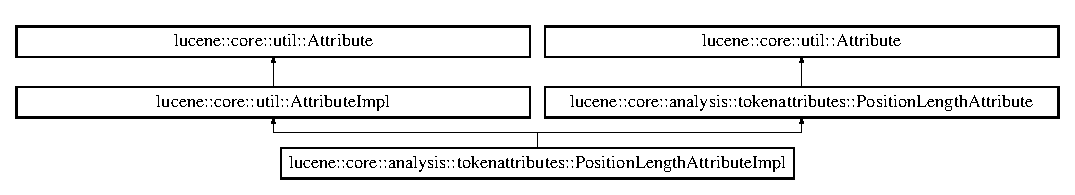
\includegraphics[height=2.176166cm]{classlucene_1_1core_1_1analysis_1_1tokenattributes_1_1PositionLengthAttributeImpl}
\end{center}
\end{figure}
\subsection*{Public Member Functions}
\begin{DoxyCompactItemize}
\item 
\mbox{\hyperlink{classlucene_1_1core_1_1analysis_1_1tokenattributes_1_1PositionLengthAttributeImpl_afcfe707b9309054f29ab710a3414a20b}{Position\+Length\+Attribute\+Impl}} ()
\item 
\mbox{\hyperlink{classlucene_1_1core_1_1analysis_1_1tokenattributes_1_1PositionLengthAttributeImpl_a2ed9d880e9632a2e444b62a1c127e713}{Position\+Length\+Attribute\+Impl}} (\mbox{\hyperlink{ZlibCrc32_8h_a2c212835823e3c54a8ab6d95c652660e}{const}} \mbox{\hyperlink{classlucene_1_1core_1_1analysis_1_1tokenattributes_1_1PositionLengthAttributeImpl}{Position\+Length\+Attribute\+Impl}} \&other)
\item 
virtual \mbox{\hyperlink{classlucene_1_1core_1_1analysis_1_1tokenattributes_1_1PositionLengthAttributeImpl_ab0cf2e31a5d40ad16b987d424344e94d}{$\sim$\+Position\+Length\+Attribute\+Impl}} ()
\item 
void \mbox{\hyperlink{classlucene_1_1core_1_1analysis_1_1tokenattributes_1_1PositionLengthAttributeImpl_aec63a5cf6bdf55b0f4c95d5b17109e5f}{Reflect\+With}} (\mbox{\hyperlink{namespacelucene_1_1core_1_1util_a7dbb701adaed055f73fb95eec83da10a}{lucene\+::core\+::util\+::\+Attribute\+Reflector}} \&reflector) override
\item 
void \mbox{\hyperlink{classlucene_1_1core_1_1analysis_1_1tokenattributes_1_1PositionLengthAttributeImpl_a0f4a9a4b9ab64ced895b8fa5b9983cbd}{Clear}} () override
\item 
bool \mbox{\hyperlink{classlucene_1_1core_1_1analysis_1_1tokenattributes_1_1PositionLengthAttributeImpl_a037d4fab2158faa6e923e78b730d0f4a}{operator==}} (\mbox{\hyperlink{ZlibCrc32_8h_a2c212835823e3c54a8ab6d95c652660e}{const}} \mbox{\hyperlink{classlucene_1_1core_1_1analysis_1_1tokenattributes_1_1PositionLengthAttributeImpl}{Position\+Length\+Attribute\+Impl}} \&other) \mbox{\hyperlink{ZlibCrc32_8h_a2c212835823e3c54a8ab6d95c652660e}{const}}
\item 
void \mbox{\hyperlink{classlucene_1_1core_1_1analysis_1_1tokenattributes_1_1PositionLengthAttributeImpl_a8b09235c697cf5157ca4351653fcbaf4}{Set\+Position\+Length}} (\mbox{\hyperlink{ZlibCrc32_8h_a2c212835823e3c54a8ab6d95c652660e}{const}} uint32\+\_\+t \mbox{\hyperlink{classlucene_1_1core_1_1analysis_1_1tokenattributes_1_1PositionLengthAttributeImpl_a12c90fb7e49f9b4043bfc09d66ef816d}{position\+\_\+length}}) override
\item 
uint32\+\_\+t \mbox{\hyperlink{classlucene_1_1core_1_1analysis_1_1tokenattributes_1_1PositionLengthAttributeImpl_a79dfa19c547152a263d601dfaf62fe9b}{Get\+Position\+Length}} () override
\item 
std\+::vector$<$ std\+::type\+\_\+index $>$ \mbox{\hyperlink{classlucene_1_1core_1_1analysis_1_1tokenattributes_1_1PositionLengthAttributeImpl_abb480ef419ad8ee6c27a50e7eda1be29}{Attributes}} () override
\item 
void \mbox{\hyperlink{classlucene_1_1core_1_1analysis_1_1tokenattributes_1_1PositionLengthAttributeImpl_a657ca7b71ea00d5ba609453d0333cafa}{Shallow\+Copy\+To}} (\mbox{\hyperlink{classlucene_1_1core_1_1util_1_1AttributeImpl}{lucene\+::core\+::util\+::\+Attribute\+Impl}} \&attr\+\_\+impl) override
\item 
\mbox{\hyperlink{classlucene_1_1core_1_1analysis_1_1tokenattributes_1_1PositionLengthAttributeImpl}{Position\+Length\+Attribute\+Impl}} \& \mbox{\hyperlink{classlucene_1_1core_1_1analysis_1_1tokenattributes_1_1PositionLengthAttributeImpl_a40bda49e6da62bc1c16e8ef11525d840}{operator=}} (\mbox{\hyperlink{ZlibCrc32_8h_a2c212835823e3c54a8ab6d95c652660e}{const}} \mbox{\hyperlink{classlucene_1_1core_1_1util_1_1AttributeImpl}{lucene\+::core\+::util\+::\+Attribute\+Impl}} \&other)
\item 
\mbox{\hyperlink{classlucene_1_1core_1_1analysis_1_1tokenattributes_1_1PositionLengthAttributeImpl}{Position\+Length\+Attribute\+Impl}} \& \mbox{\hyperlink{classlucene_1_1core_1_1analysis_1_1tokenattributes_1_1PositionLengthAttributeImpl_a01cf482ffe511eaa7de8b8c19690f4d7}{operator=}} (\mbox{\hyperlink{ZlibCrc32_8h_a2c212835823e3c54a8ab6d95c652660e}{const}} \mbox{\hyperlink{classlucene_1_1core_1_1analysis_1_1tokenattributes_1_1PositionLengthAttributeImpl}{Position\+Length\+Attribute\+Impl}} \&other)
\item 
\mbox{\hyperlink{classlucene_1_1core_1_1util_1_1AttributeImpl}{lucene\+::core\+::util\+::\+Attribute\+Impl}} $\ast$ \mbox{\hyperlink{classlucene_1_1core_1_1analysis_1_1tokenattributes_1_1PositionLengthAttributeImpl_a8880c22ea7f0cc06c2f7ed98900286aa}{Clone}} () override
\end{DoxyCompactItemize}
\subsection*{Private Attributes}
\begin{DoxyCompactItemize}
\item 
uint32\+\_\+t \mbox{\hyperlink{classlucene_1_1core_1_1analysis_1_1tokenattributes_1_1PositionLengthAttributeImpl_a12c90fb7e49f9b4043bfc09d66ef816d}{position\+\_\+length}}
\end{DoxyCompactItemize}
\subsection*{Additional Inherited Members}


\subsection{Constructor \& Destructor Documentation}
\mbox{\Hypertarget{classlucene_1_1core_1_1analysis_1_1tokenattributes_1_1PositionLengthAttributeImpl_afcfe707b9309054f29ab710a3414a20b}\label{classlucene_1_1core_1_1analysis_1_1tokenattributes_1_1PositionLengthAttributeImpl_afcfe707b9309054f29ab710a3414a20b}} 
\index{lucene\+::core\+::analysis\+::tokenattributes\+::\+Position\+Length\+Attribute\+Impl@{lucene\+::core\+::analysis\+::tokenattributes\+::\+Position\+Length\+Attribute\+Impl}!Position\+Length\+Attribute\+Impl@{Position\+Length\+Attribute\+Impl}}
\index{Position\+Length\+Attribute\+Impl@{Position\+Length\+Attribute\+Impl}!lucene\+::core\+::analysis\+::tokenattributes\+::\+Position\+Length\+Attribute\+Impl@{lucene\+::core\+::analysis\+::tokenattributes\+::\+Position\+Length\+Attribute\+Impl}}
\subsubsection{\texorpdfstring{Position\+Length\+Attribute\+Impl()}{PositionLengthAttributeImpl()}\hspace{0.1cm}{\footnotesize\ttfamily [1/2]}}
{\footnotesize\ttfamily Position\+Length\+Attribute\+Impl\+::\+Position\+Length\+Attribute\+Impl (\begin{DoxyParamCaption}{ }\end{DoxyParamCaption})}

\mbox{\hyperlink{classlucene_1_1core_1_1analysis_1_1tokenattributes_1_1PositionLengthAttributeImpl}{Position\+Length\+Attribute\+Impl}} \mbox{\Hypertarget{classlucene_1_1core_1_1analysis_1_1tokenattributes_1_1PositionLengthAttributeImpl_a2ed9d880e9632a2e444b62a1c127e713}\label{classlucene_1_1core_1_1analysis_1_1tokenattributes_1_1PositionLengthAttributeImpl_a2ed9d880e9632a2e444b62a1c127e713}} 
\index{lucene\+::core\+::analysis\+::tokenattributes\+::\+Position\+Length\+Attribute\+Impl@{lucene\+::core\+::analysis\+::tokenattributes\+::\+Position\+Length\+Attribute\+Impl}!Position\+Length\+Attribute\+Impl@{Position\+Length\+Attribute\+Impl}}
\index{Position\+Length\+Attribute\+Impl@{Position\+Length\+Attribute\+Impl}!lucene\+::core\+::analysis\+::tokenattributes\+::\+Position\+Length\+Attribute\+Impl@{lucene\+::core\+::analysis\+::tokenattributes\+::\+Position\+Length\+Attribute\+Impl}}
\subsubsection{\texorpdfstring{Position\+Length\+Attribute\+Impl()}{PositionLengthAttributeImpl()}\hspace{0.1cm}{\footnotesize\ttfamily [2/2]}}
{\footnotesize\ttfamily Position\+Length\+Attribute\+Impl\+::\+Position\+Length\+Attribute\+Impl (\begin{DoxyParamCaption}\item[{\mbox{\hyperlink{ZlibCrc32_8h_a2c212835823e3c54a8ab6d95c652660e}{const}} \mbox{\hyperlink{classlucene_1_1core_1_1analysis_1_1tokenattributes_1_1PositionLengthAttributeImpl}{Position\+Length\+Attribute\+Impl}} \&}]{other }\end{DoxyParamCaption})}

\mbox{\Hypertarget{classlucene_1_1core_1_1analysis_1_1tokenattributes_1_1PositionLengthAttributeImpl_ab0cf2e31a5d40ad16b987d424344e94d}\label{classlucene_1_1core_1_1analysis_1_1tokenattributes_1_1PositionLengthAttributeImpl_ab0cf2e31a5d40ad16b987d424344e94d}} 
\index{lucene\+::core\+::analysis\+::tokenattributes\+::\+Position\+Length\+Attribute\+Impl@{lucene\+::core\+::analysis\+::tokenattributes\+::\+Position\+Length\+Attribute\+Impl}!````~Position\+Length\+Attribute\+Impl@{$\sim$\+Position\+Length\+Attribute\+Impl}}
\index{````~Position\+Length\+Attribute\+Impl@{$\sim$\+Position\+Length\+Attribute\+Impl}!lucene\+::core\+::analysis\+::tokenattributes\+::\+Position\+Length\+Attribute\+Impl@{lucene\+::core\+::analysis\+::tokenattributes\+::\+Position\+Length\+Attribute\+Impl}}
\subsubsection{\texorpdfstring{$\sim$\+Position\+Length\+Attribute\+Impl()}{~PositionLengthAttributeImpl()}}
{\footnotesize\ttfamily Position\+Length\+Attribute\+Impl\+::$\sim$\+Position\+Length\+Attribute\+Impl (\begin{DoxyParamCaption}{ }\end{DoxyParamCaption})\hspace{0.3cm}{\ttfamily [virtual]}}



\subsection{Member Function Documentation}
\mbox{\Hypertarget{classlucene_1_1core_1_1analysis_1_1tokenattributes_1_1PositionLengthAttributeImpl_abb480ef419ad8ee6c27a50e7eda1be29}\label{classlucene_1_1core_1_1analysis_1_1tokenattributes_1_1PositionLengthAttributeImpl_abb480ef419ad8ee6c27a50e7eda1be29}} 
\index{lucene\+::core\+::analysis\+::tokenattributes\+::\+Position\+Length\+Attribute\+Impl@{lucene\+::core\+::analysis\+::tokenattributes\+::\+Position\+Length\+Attribute\+Impl}!Attributes@{Attributes}}
\index{Attributes@{Attributes}!lucene\+::core\+::analysis\+::tokenattributes\+::\+Position\+Length\+Attribute\+Impl@{lucene\+::core\+::analysis\+::tokenattributes\+::\+Position\+Length\+Attribute\+Impl}}
\subsubsection{\texorpdfstring{Attributes()}{Attributes()}}
{\footnotesize\ttfamily std\+::vector$<$ std\+::type\+\_\+index $>$ Position\+Length\+Attribute\+Impl\+::\+Attributes (\begin{DoxyParamCaption}{ }\end{DoxyParamCaption})\hspace{0.3cm}{\ttfamily [override]}, {\ttfamily [virtual]}}



Implements \mbox{\hyperlink{classlucene_1_1core_1_1util_1_1AttributeImpl_ac0631e6a7a11044883bc97447716d7cc}{lucene\+::core\+::util\+::\+Attribute\+Impl}}.

\mbox{\Hypertarget{classlucene_1_1core_1_1analysis_1_1tokenattributes_1_1PositionLengthAttributeImpl_a0f4a9a4b9ab64ced895b8fa5b9983cbd}\label{classlucene_1_1core_1_1analysis_1_1tokenattributes_1_1PositionLengthAttributeImpl_a0f4a9a4b9ab64ced895b8fa5b9983cbd}} 
\index{lucene\+::core\+::analysis\+::tokenattributes\+::\+Position\+Length\+Attribute\+Impl@{lucene\+::core\+::analysis\+::tokenattributes\+::\+Position\+Length\+Attribute\+Impl}!Clear@{Clear}}
\index{Clear@{Clear}!lucene\+::core\+::analysis\+::tokenattributes\+::\+Position\+Length\+Attribute\+Impl@{lucene\+::core\+::analysis\+::tokenattributes\+::\+Position\+Length\+Attribute\+Impl}}
\subsubsection{\texorpdfstring{Clear()}{Clear()}}
{\footnotesize\ttfamily void Position\+Length\+Attribute\+Impl\+::\+Clear (\begin{DoxyParamCaption}{ }\end{DoxyParamCaption})\hspace{0.3cm}{\ttfamily [override]}, {\ttfamily [virtual]}}



Implements \mbox{\hyperlink{classlucene_1_1core_1_1util_1_1AttributeImpl_a04897a00a902f7a345dd44bbc4b482a8}{lucene\+::core\+::util\+::\+Attribute\+Impl}}.

\mbox{\Hypertarget{classlucene_1_1core_1_1analysis_1_1tokenattributes_1_1PositionLengthAttributeImpl_a8880c22ea7f0cc06c2f7ed98900286aa}\label{classlucene_1_1core_1_1analysis_1_1tokenattributes_1_1PositionLengthAttributeImpl_a8880c22ea7f0cc06c2f7ed98900286aa}} 
\index{lucene\+::core\+::analysis\+::tokenattributes\+::\+Position\+Length\+Attribute\+Impl@{lucene\+::core\+::analysis\+::tokenattributes\+::\+Position\+Length\+Attribute\+Impl}!Clone@{Clone}}
\index{Clone@{Clone}!lucene\+::core\+::analysis\+::tokenattributes\+::\+Position\+Length\+Attribute\+Impl@{lucene\+::core\+::analysis\+::tokenattributes\+::\+Position\+Length\+Attribute\+Impl}}
\subsubsection{\texorpdfstring{Clone()}{Clone()}}
{\footnotesize\ttfamily \mbox{\hyperlink{classlucene_1_1core_1_1util_1_1AttributeImpl}{Attribute\+Impl}} $\ast$ Position\+Length\+Attribute\+Impl\+::\+Clone (\begin{DoxyParamCaption}{ }\end{DoxyParamCaption})\hspace{0.3cm}{\ttfamily [override]}, {\ttfamily [virtual]}}



Implements \mbox{\hyperlink{classlucene_1_1core_1_1util_1_1AttributeImpl_a135318ad4c7c17b3d85e625e32fb42cd}{lucene\+::core\+::util\+::\+Attribute\+Impl}}.

\mbox{\Hypertarget{classlucene_1_1core_1_1analysis_1_1tokenattributes_1_1PositionLengthAttributeImpl_a79dfa19c547152a263d601dfaf62fe9b}\label{classlucene_1_1core_1_1analysis_1_1tokenattributes_1_1PositionLengthAttributeImpl_a79dfa19c547152a263d601dfaf62fe9b}} 
\index{lucene\+::core\+::analysis\+::tokenattributes\+::\+Position\+Length\+Attribute\+Impl@{lucene\+::core\+::analysis\+::tokenattributes\+::\+Position\+Length\+Attribute\+Impl}!Get\+Position\+Length@{Get\+Position\+Length}}
\index{Get\+Position\+Length@{Get\+Position\+Length}!lucene\+::core\+::analysis\+::tokenattributes\+::\+Position\+Length\+Attribute\+Impl@{lucene\+::core\+::analysis\+::tokenattributes\+::\+Position\+Length\+Attribute\+Impl}}
\subsubsection{\texorpdfstring{Get\+Position\+Length()}{GetPositionLength()}}
{\footnotesize\ttfamily uint32\+\_\+t Position\+Length\+Attribute\+Impl\+::\+Get\+Position\+Length (\begin{DoxyParamCaption}{ }\end{DoxyParamCaption})\hspace{0.3cm}{\ttfamily [override]}, {\ttfamily [virtual]}}



Implements \mbox{\hyperlink{classlucene_1_1core_1_1analysis_1_1tokenattributes_1_1PositionLengthAttribute_a6325424899959bb480f161e0d5490bfd}{lucene\+::core\+::analysis\+::tokenattributes\+::\+Position\+Length\+Attribute}}.

\mbox{\Hypertarget{classlucene_1_1core_1_1analysis_1_1tokenattributes_1_1PositionLengthAttributeImpl_a40bda49e6da62bc1c16e8ef11525d840}\label{classlucene_1_1core_1_1analysis_1_1tokenattributes_1_1PositionLengthAttributeImpl_a40bda49e6da62bc1c16e8ef11525d840}} 
\index{lucene\+::core\+::analysis\+::tokenattributes\+::\+Position\+Length\+Attribute\+Impl@{lucene\+::core\+::analysis\+::tokenattributes\+::\+Position\+Length\+Attribute\+Impl}!operator=@{operator=}}
\index{operator=@{operator=}!lucene\+::core\+::analysis\+::tokenattributes\+::\+Position\+Length\+Attribute\+Impl@{lucene\+::core\+::analysis\+::tokenattributes\+::\+Position\+Length\+Attribute\+Impl}}
\subsubsection{\texorpdfstring{operator=()}{operator=()}\hspace{0.1cm}{\footnotesize\ttfamily [1/2]}}
{\footnotesize\ttfamily \mbox{\hyperlink{classlucene_1_1core_1_1analysis_1_1tokenattributes_1_1PositionLengthAttributeImpl}{Position\+Length\+Attribute\+Impl}} \& Position\+Length\+Attribute\+Impl\+::operator= (\begin{DoxyParamCaption}\item[{\mbox{\hyperlink{ZlibCrc32_8h_a2c212835823e3c54a8ab6d95c652660e}{const}} \mbox{\hyperlink{classlucene_1_1core_1_1util_1_1AttributeImpl}{lucene\+::core\+::util\+::\+Attribute\+Impl}} \&}]{other }\end{DoxyParamCaption})\hspace{0.3cm}{\ttfamily [virtual]}}



Implements \mbox{\hyperlink{classlucene_1_1core_1_1util_1_1AttributeImpl_ab032e399d03ce2f58c76881cf2b92325}{lucene\+::core\+::util\+::\+Attribute\+Impl}}.

\mbox{\Hypertarget{classlucene_1_1core_1_1analysis_1_1tokenattributes_1_1PositionLengthAttributeImpl_a01cf482ffe511eaa7de8b8c19690f4d7}\label{classlucene_1_1core_1_1analysis_1_1tokenattributes_1_1PositionLengthAttributeImpl_a01cf482ffe511eaa7de8b8c19690f4d7}} 
\index{lucene\+::core\+::analysis\+::tokenattributes\+::\+Position\+Length\+Attribute\+Impl@{lucene\+::core\+::analysis\+::tokenattributes\+::\+Position\+Length\+Attribute\+Impl}!operator=@{operator=}}
\index{operator=@{operator=}!lucene\+::core\+::analysis\+::tokenattributes\+::\+Position\+Length\+Attribute\+Impl@{lucene\+::core\+::analysis\+::tokenattributes\+::\+Position\+Length\+Attribute\+Impl}}
\subsubsection{\texorpdfstring{operator=()}{operator=()}\hspace{0.1cm}{\footnotesize\ttfamily [2/2]}}
{\footnotesize\ttfamily \mbox{\hyperlink{classlucene_1_1core_1_1analysis_1_1tokenattributes_1_1PositionLengthAttributeImpl}{Position\+Length\+Attribute\+Impl}} \& Position\+Length\+Attribute\+Impl\+::operator= (\begin{DoxyParamCaption}\item[{\mbox{\hyperlink{ZlibCrc32_8h_a2c212835823e3c54a8ab6d95c652660e}{const}} \mbox{\hyperlink{classlucene_1_1core_1_1analysis_1_1tokenattributes_1_1PositionLengthAttributeImpl}{Position\+Length\+Attribute\+Impl}} \&}]{other }\end{DoxyParamCaption})}

\mbox{\Hypertarget{classlucene_1_1core_1_1analysis_1_1tokenattributes_1_1PositionLengthAttributeImpl_a037d4fab2158faa6e923e78b730d0f4a}\label{classlucene_1_1core_1_1analysis_1_1tokenattributes_1_1PositionLengthAttributeImpl_a037d4fab2158faa6e923e78b730d0f4a}} 
\index{lucene\+::core\+::analysis\+::tokenattributes\+::\+Position\+Length\+Attribute\+Impl@{lucene\+::core\+::analysis\+::tokenattributes\+::\+Position\+Length\+Attribute\+Impl}!operator==@{operator==}}
\index{operator==@{operator==}!lucene\+::core\+::analysis\+::tokenattributes\+::\+Position\+Length\+Attribute\+Impl@{lucene\+::core\+::analysis\+::tokenattributes\+::\+Position\+Length\+Attribute\+Impl}}
\subsubsection{\texorpdfstring{operator==()}{operator==()}}
{\footnotesize\ttfamily bool Position\+Length\+Attribute\+Impl\+::operator== (\begin{DoxyParamCaption}\item[{\mbox{\hyperlink{ZlibCrc32_8h_a2c212835823e3c54a8ab6d95c652660e}{const}} \mbox{\hyperlink{classlucene_1_1core_1_1analysis_1_1tokenattributes_1_1PositionLengthAttributeImpl}{Position\+Length\+Attribute\+Impl}} \&}]{other }\end{DoxyParamCaption}) const}

\mbox{\Hypertarget{classlucene_1_1core_1_1analysis_1_1tokenattributes_1_1PositionLengthAttributeImpl_aec63a5cf6bdf55b0f4c95d5b17109e5f}\label{classlucene_1_1core_1_1analysis_1_1tokenattributes_1_1PositionLengthAttributeImpl_aec63a5cf6bdf55b0f4c95d5b17109e5f}} 
\index{lucene\+::core\+::analysis\+::tokenattributes\+::\+Position\+Length\+Attribute\+Impl@{lucene\+::core\+::analysis\+::tokenattributes\+::\+Position\+Length\+Attribute\+Impl}!Reflect\+With@{Reflect\+With}}
\index{Reflect\+With@{Reflect\+With}!lucene\+::core\+::analysis\+::tokenattributes\+::\+Position\+Length\+Attribute\+Impl@{lucene\+::core\+::analysis\+::tokenattributes\+::\+Position\+Length\+Attribute\+Impl}}
\subsubsection{\texorpdfstring{Reflect\+With()}{ReflectWith()}}
{\footnotesize\ttfamily void Position\+Length\+Attribute\+Impl\+::\+Reflect\+With (\begin{DoxyParamCaption}\item[{\mbox{\hyperlink{namespacelucene_1_1core_1_1util_a7dbb701adaed055f73fb95eec83da10a}{lucene\+::core\+::util\+::\+Attribute\+Reflector}} \&}]{reflector }\end{DoxyParamCaption})\hspace{0.3cm}{\ttfamily [override]}, {\ttfamily [virtual]}}



Implements \mbox{\hyperlink{classlucene_1_1core_1_1util_1_1AttributeImpl_a84d34275fb1ed67ac36fad7ff6388096}{lucene\+::core\+::util\+::\+Attribute\+Impl}}.

\mbox{\Hypertarget{classlucene_1_1core_1_1analysis_1_1tokenattributes_1_1PositionLengthAttributeImpl_a8b09235c697cf5157ca4351653fcbaf4}\label{classlucene_1_1core_1_1analysis_1_1tokenattributes_1_1PositionLengthAttributeImpl_a8b09235c697cf5157ca4351653fcbaf4}} 
\index{lucene\+::core\+::analysis\+::tokenattributes\+::\+Position\+Length\+Attribute\+Impl@{lucene\+::core\+::analysis\+::tokenattributes\+::\+Position\+Length\+Attribute\+Impl}!Set\+Position\+Length@{Set\+Position\+Length}}
\index{Set\+Position\+Length@{Set\+Position\+Length}!lucene\+::core\+::analysis\+::tokenattributes\+::\+Position\+Length\+Attribute\+Impl@{lucene\+::core\+::analysis\+::tokenattributes\+::\+Position\+Length\+Attribute\+Impl}}
\subsubsection{\texorpdfstring{Set\+Position\+Length()}{SetPositionLength()}}
{\footnotesize\ttfamily void Position\+Length\+Attribute\+Impl\+::\+Set\+Position\+Length (\begin{DoxyParamCaption}\item[{\mbox{\hyperlink{ZlibCrc32_8h_a2c212835823e3c54a8ab6d95c652660e}{const}} uint32\+\_\+t}]{position\+\_\+length }\end{DoxyParamCaption})\hspace{0.3cm}{\ttfamily [override]}, {\ttfamily [virtual]}}



Implements \mbox{\hyperlink{classlucene_1_1core_1_1analysis_1_1tokenattributes_1_1PositionLengthAttribute_a514415965bae0dd392cbb8d65ea4d808}{lucene\+::core\+::analysis\+::tokenattributes\+::\+Position\+Length\+Attribute}}.

\mbox{\Hypertarget{classlucene_1_1core_1_1analysis_1_1tokenattributes_1_1PositionLengthAttributeImpl_a657ca7b71ea00d5ba609453d0333cafa}\label{classlucene_1_1core_1_1analysis_1_1tokenattributes_1_1PositionLengthAttributeImpl_a657ca7b71ea00d5ba609453d0333cafa}} 
\index{lucene\+::core\+::analysis\+::tokenattributes\+::\+Position\+Length\+Attribute\+Impl@{lucene\+::core\+::analysis\+::tokenattributes\+::\+Position\+Length\+Attribute\+Impl}!Shallow\+Copy\+To@{Shallow\+Copy\+To}}
\index{Shallow\+Copy\+To@{Shallow\+Copy\+To}!lucene\+::core\+::analysis\+::tokenattributes\+::\+Position\+Length\+Attribute\+Impl@{lucene\+::core\+::analysis\+::tokenattributes\+::\+Position\+Length\+Attribute\+Impl}}
\subsubsection{\texorpdfstring{Shallow\+Copy\+To()}{ShallowCopyTo()}}
{\footnotesize\ttfamily void Position\+Length\+Attribute\+Impl\+::\+Shallow\+Copy\+To (\begin{DoxyParamCaption}\item[{\mbox{\hyperlink{classlucene_1_1core_1_1util_1_1AttributeImpl}{lucene\+::core\+::util\+::\+Attribute\+Impl}} \&}]{attr\+\_\+impl }\end{DoxyParamCaption})\hspace{0.3cm}{\ttfamily [override]}, {\ttfamily [virtual]}}



Implements \mbox{\hyperlink{classlucene_1_1core_1_1util_1_1AttributeImpl_a010e8937832f53139c8fe42757476895}{lucene\+::core\+::util\+::\+Attribute\+Impl}}.



\subsection{Member Data Documentation}
\mbox{\Hypertarget{classlucene_1_1core_1_1analysis_1_1tokenattributes_1_1PositionLengthAttributeImpl_a12c90fb7e49f9b4043bfc09d66ef816d}\label{classlucene_1_1core_1_1analysis_1_1tokenattributes_1_1PositionLengthAttributeImpl_a12c90fb7e49f9b4043bfc09d66ef816d}} 
\index{lucene\+::core\+::analysis\+::tokenattributes\+::\+Position\+Length\+Attribute\+Impl@{lucene\+::core\+::analysis\+::tokenattributes\+::\+Position\+Length\+Attribute\+Impl}!position\+\_\+length@{position\+\_\+length}}
\index{position\+\_\+length@{position\+\_\+length}!lucene\+::core\+::analysis\+::tokenattributes\+::\+Position\+Length\+Attribute\+Impl@{lucene\+::core\+::analysis\+::tokenattributes\+::\+Position\+Length\+Attribute\+Impl}}
\subsubsection{\texorpdfstring{position\+\_\+length}{position\_length}}
{\footnotesize\ttfamily uint32\+\_\+t lucene\+::core\+::analysis\+::tokenattributes\+::\+Position\+Length\+Attribute\+Impl\+::position\+\_\+length\hspace{0.3cm}{\ttfamily [private]}}



The documentation for this class was generated from the following files\+:\begin{DoxyCompactItemize}
\item 
Analysis/\mbox{\hyperlink{AttributeImpl_8h}{Attribute\+Impl.\+h}}\item 
Analysis/\mbox{\hyperlink{AttributeImpl_8cpp}{Attribute\+Impl.\+cpp}}\end{DoxyCompactItemize}

\hypertarget{classlucene_1_1core_1_1analysis_1_1Reader}{}\section{lucene\+:\+:core\+:\+:analysis\+:\+:Reader Class Reference}
\label{classlucene_1_1core_1_1analysis_1_1Reader}\index{lucene\+::core\+::analysis\+::\+Reader@{lucene\+::core\+::analysis\+::\+Reader}}


{\ttfamily \#include $<$Reader.\+h$>$}

Inheritance diagram for lucene\+:\+:core\+:\+:analysis\+:\+:Reader\+:\begin{figure}[H]
\begin{center}
\leavevmode
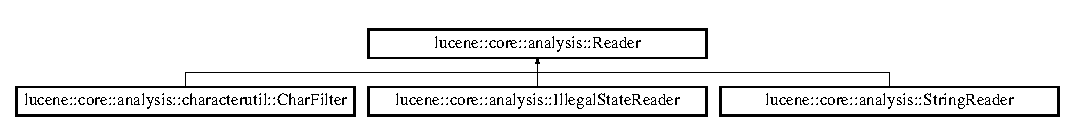
\includegraphics[height=1.323877cm]{classlucene_1_1core_1_1analysis_1_1Reader}
\end{center}
\end{figure}
\subsection*{Public Member Functions}
\begin{DoxyCompactItemize}
\item 
virtual \mbox{\hyperlink{classlucene_1_1core_1_1analysis_1_1Reader_a78089542fd27a0ac2df6702fffe8725c}{$\sim$\+Reader}} ()
\item 
virtual int \mbox{\hyperlink{classlucene_1_1core_1_1analysis_1_1Reader_ae8e04911b6a4c06bb026ca6e74071cb2}{Read}} ()=0
\item 
virtual void \mbox{\hyperlink{classlucene_1_1core_1_1analysis_1_1Reader_a475ba046fd74e43a1cce4c4702c791c2}{Read\+Line}} (std\+::string \&line)=0
\item 
virtual int \mbox{\hyperlink{classlucene_1_1core_1_1analysis_1_1Reader_a986e25a49a947dc113a22c6de033ebe9}{Read}} (char $\ast$cstr, const uint32\+\_\+t off, const uint32\+\_\+t len)=0
\item 
virtual void \mbox{\hyperlink{classlucene_1_1core_1_1analysis_1_1Reader_a3bd8e9f3e1d07d698bccabde41970219}{Skip}} (const uint64\+\_\+t n)=0
\item 
virtual bool \mbox{\hyperlink{classlucene_1_1core_1_1analysis_1_1Reader_a230fae02ca4a63de33fdaad6f9aafd96}{Mark\+Supported}} ()=0
\item 
virtual void \mbox{\hyperlink{classlucene_1_1core_1_1analysis_1_1Reader_a0b60b07a3f65098a50f10f6618097527}{Mark}} (const uint32\+\_\+t read\+\_\+ahead\+\_\+limit)=0
\item 
virtual void \mbox{\hyperlink{classlucene_1_1core_1_1analysis_1_1Reader_a5299f5469ce4ea9812ec79a59667945a}{Reset}} ()=0
\item 
virtual void \mbox{\hyperlink{classlucene_1_1core_1_1analysis_1_1Reader_a4be7e96dccdd3e276e3450e3ad7a70f4}{Close}} ()=0
\item 
virtual bool \mbox{\hyperlink{classlucene_1_1core_1_1analysis_1_1Reader_af7a24f3904f9c40e9c5c204b3434f1f7}{Eof}} ()=0
\end{DoxyCompactItemize}


\subsection{Constructor \& Destructor Documentation}
\mbox{\Hypertarget{classlucene_1_1core_1_1analysis_1_1Reader_a78089542fd27a0ac2df6702fffe8725c}\label{classlucene_1_1core_1_1analysis_1_1Reader_a78089542fd27a0ac2df6702fffe8725c}} 
\index{lucene\+::core\+::analysis\+::\+Reader@{lucene\+::core\+::analysis\+::\+Reader}!````~Reader@{$\sim$\+Reader}}
\index{````~Reader@{$\sim$\+Reader}!lucene\+::core\+::analysis\+::\+Reader@{lucene\+::core\+::analysis\+::\+Reader}}
\subsubsection{\texorpdfstring{$\sim$\+Reader()}{~Reader()}}
{\footnotesize\ttfamily Reader\+::$\sim$\+Reader (\begin{DoxyParamCaption}{ }\end{DoxyParamCaption})\hspace{0.3cm}{\ttfamily [virtual]}}

\mbox{\hyperlink{classlucene_1_1core_1_1analysis_1_1Reader}{Reader}} 

\subsection{Member Function Documentation}
\mbox{\Hypertarget{classlucene_1_1core_1_1analysis_1_1Reader_a4be7e96dccdd3e276e3450e3ad7a70f4}\label{classlucene_1_1core_1_1analysis_1_1Reader_a4be7e96dccdd3e276e3450e3ad7a70f4}} 
\index{lucene\+::core\+::analysis\+::\+Reader@{lucene\+::core\+::analysis\+::\+Reader}!Close@{Close}}
\index{Close@{Close}!lucene\+::core\+::analysis\+::\+Reader@{lucene\+::core\+::analysis\+::\+Reader}}
\subsubsection{\texorpdfstring{Close()}{Close()}}
{\footnotesize\ttfamily virtual void lucene\+::core\+::analysis\+::\+Reader\+::\+Close (\begin{DoxyParamCaption}{ }\end{DoxyParamCaption})\hspace{0.3cm}{\ttfamily [pure virtual]}}



Implemented in \mbox{\hyperlink{classlucene_1_1core_1_1analysis_1_1StringReader_ac2938d531e7842abb8423149982328e3}{lucene\+::core\+::analysis\+::\+String\+Reader}}, \mbox{\hyperlink{classlucene_1_1core_1_1analysis_1_1IllegalStateReader_aa92b3c9c3da611e2e44c3edf4078dbe6}{lucene\+::core\+::analysis\+::\+Illegal\+State\+Reader}}, and \mbox{\hyperlink{classlucene_1_1core_1_1analysis_1_1characterutil_1_1CharFilter_a47ff3dc61979b80927ed5779cb55bd09}{lucene\+::core\+::analysis\+::characterutil\+::\+Char\+Filter}}.

\mbox{\Hypertarget{classlucene_1_1core_1_1analysis_1_1Reader_af7a24f3904f9c40e9c5c204b3434f1f7}\label{classlucene_1_1core_1_1analysis_1_1Reader_af7a24f3904f9c40e9c5c204b3434f1f7}} 
\index{lucene\+::core\+::analysis\+::\+Reader@{lucene\+::core\+::analysis\+::\+Reader}!Eof@{Eof}}
\index{Eof@{Eof}!lucene\+::core\+::analysis\+::\+Reader@{lucene\+::core\+::analysis\+::\+Reader}}
\subsubsection{\texorpdfstring{Eof()}{Eof()}}
{\footnotesize\ttfamily virtual bool lucene\+::core\+::analysis\+::\+Reader\+::\+Eof (\begin{DoxyParamCaption}{ }\end{DoxyParamCaption})\hspace{0.3cm}{\ttfamily [pure virtual]}}



Implemented in \mbox{\hyperlink{classlucene_1_1core_1_1analysis_1_1StringReader_a7697e462ff19e3e8fa135e38fa3e4999}{lucene\+::core\+::analysis\+::\+String\+Reader}}, and \mbox{\hyperlink{classlucene_1_1core_1_1analysis_1_1IllegalStateReader_a0f3665a702d4b01dc3298e547379339a}{lucene\+::core\+::analysis\+::\+Illegal\+State\+Reader}}.

\mbox{\Hypertarget{classlucene_1_1core_1_1analysis_1_1Reader_a0b60b07a3f65098a50f10f6618097527}\label{classlucene_1_1core_1_1analysis_1_1Reader_a0b60b07a3f65098a50f10f6618097527}} 
\index{lucene\+::core\+::analysis\+::\+Reader@{lucene\+::core\+::analysis\+::\+Reader}!Mark@{Mark}}
\index{Mark@{Mark}!lucene\+::core\+::analysis\+::\+Reader@{lucene\+::core\+::analysis\+::\+Reader}}
\subsubsection{\texorpdfstring{Mark()}{Mark()}}
{\footnotesize\ttfamily virtual void lucene\+::core\+::analysis\+::\+Reader\+::\+Mark (\begin{DoxyParamCaption}\item[{const uint32\+\_\+t}]{read\+\_\+ahead\+\_\+limit }\end{DoxyParamCaption})\hspace{0.3cm}{\ttfamily [pure virtual]}}



Implemented in \mbox{\hyperlink{classlucene_1_1core_1_1analysis_1_1StringReader_a0ba42881881e4790dae54bc1c01063f5}{lucene\+::core\+::analysis\+::\+String\+Reader}}, and \mbox{\hyperlink{classlucene_1_1core_1_1analysis_1_1IllegalStateReader_a96a8cb65743ac1a4db9633b2e0d203fb}{lucene\+::core\+::analysis\+::\+Illegal\+State\+Reader}}.

\mbox{\Hypertarget{classlucene_1_1core_1_1analysis_1_1Reader_a230fae02ca4a63de33fdaad6f9aafd96}\label{classlucene_1_1core_1_1analysis_1_1Reader_a230fae02ca4a63de33fdaad6f9aafd96}} 
\index{lucene\+::core\+::analysis\+::\+Reader@{lucene\+::core\+::analysis\+::\+Reader}!Mark\+Supported@{Mark\+Supported}}
\index{Mark\+Supported@{Mark\+Supported}!lucene\+::core\+::analysis\+::\+Reader@{lucene\+::core\+::analysis\+::\+Reader}}
\subsubsection{\texorpdfstring{Mark\+Supported()}{MarkSupported()}}
{\footnotesize\ttfamily virtual bool lucene\+::core\+::analysis\+::\+Reader\+::\+Mark\+Supported (\begin{DoxyParamCaption}{ }\end{DoxyParamCaption})\hspace{0.3cm}{\ttfamily [pure virtual]}}



Implemented in \mbox{\hyperlink{classlucene_1_1core_1_1analysis_1_1StringReader_a1b9e55036f01d10650fd4026f23da629}{lucene\+::core\+::analysis\+::\+String\+Reader}}, and \mbox{\hyperlink{classlucene_1_1core_1_1analysis_1_1IllegalStateReader_ae2de5e9375664ca55c80b224ac3cd998}{lucene\+::core\+::analysis\+::\+Illegal\+State\+Reader}}.

\mbox{\Hypertarget{classlucene_1_1core_1_1analysis_1_1Reader_ae8e04911b6a4c06bb026ca6e74071cb2}\label{classlucene_1_1core_1_1analysis_1_1Reader_ae8e04911b6a4c06bb026ca6e74071cb2}} 
\index{lucene\+::core\+::analysis\+::\+Reader@{lucene\+::core\+::analysis\+::\+Reader}!Read@{Read}}
\index{Read@{Read}!lucene\+::core\+::analysis\+::\+Reader@{lucene\+::core\+::analysis\+::\+Reader}}
\subsubsection{\texorpdfstring{Read()}{Read()}\hspace{0.1cm}{\footnotesize\ttfamily [1/2]}}
{\footnotesize\ttfamily virtual int lucene\+::core\+::analysis\+::\+Reader\+::\+Read (\begin{DoxyParamCaption}{ }\end{DoxyParamCaption})\hspace{0.3cm}{\ttfamily [pure virtual]}}



Implemented in \mbox{\hyperlink{classlucene_1_1core_1_1analysis_1_1StringReader_ac9c1bb033ee4f5862e47e90c422d3381}{lucene\+::core\+::analysis\+::\+String\+Reader}}, and \mbox{\hyperlink{classlucene_1_1core_1_1analysis_1_1IllegalStateReader_a9bca98f676ac3d0eeadfd4a2cc78d764}{lucene\+::core\+::analysis\+::\+Illegal\+State\+Reader}}.

\mbox{\Hypertarget{classlucene_1_1core_1_1analysis_1_1Reader_a986e25a49a947dc113a22c6de033ebe9}\label{classlucene_1_1core_1_1analysis_1_1Reader_a986e25a49a947dc113a22c6de033ebe9}} 
\index{lucene\+::core\+::analysis\+::\+Reader@{lucene\+::core\+::analysis\+::\+Reader}!Read@{Read}}
\index{Read@{Read}!lucene\+::core\+::analysis\+::\+Reader@{lucene\+::core\+::analysis\+::\+Reader}}
\subsubsection{\texorpdfstring{Read()}{Read()}\hspace{0.1cm}{\footnotesize\ttfamily [2/2]}}
{\footnotesize\ttfamily virtual int lucene\+::core\+::analysis\+::\+Reader\+::\+Read (\begin{DoxyParamCaption}\item[{char $\ast$}]{cstr,  }\item[{const uint32\+\_\+t}]{off,  }\item[{const uint32\+\_\+t}]{len }\end{DoxyParamCaption})\hspace{0.3cm}{\ttfamily [pure virtual]}}



Implemented in \mbox{\hyperlink{classlucene_1_1core_1_1analysis_1_1StringReader_ab048d6d6d759175eeda5321a480995c3}{lucene\+::core\+::analysis\+::\+String\+Reader}}, and \mbox{\hyperlink{classlucene_1_1core_1_1analysis_1_1IllegalStateReader_a8017ca4fc795b71e16bb87d4a24bdfa9}{lucene\+::core\+::analysis\+::\+Illegal\+State\+Reader}}.

\mbox{\Hypertarget{classlucene_1_1core_1_1analysis_1_1Reader_a475ba046fd74e43a1cce4c4702c791c2}\label{classlucene_1_1core_1_1analysis_1_1Reader_a475ba046fd74e43a1cce4c4702c791c2}} 
\index{lucene\+::core\+::analysis\+::\+Reader@{lucene\+::core\+::analysis\+::\+Reader}!Read\+Line@{Read\+Line}}
\index{Read\+Line@{Read\+Line}!lucene\+::core\+::analysis\+::\+Reader@{lucene\+::core\+::analysis\+::\+Reader}}
\subsubsection{\texorpdfstring{Read\+Line()}{ReadLine()}}
{\footnotesize\ttfamily virtual void lucene\+::core\+::analysis\+::\+Reader\+::\+Read\+Line (\begin{DoxyParamCaption}\item[{std\+::string \&}]{line }\end{DoxyParamCaption})\hspace{0.3cm}{\ttfamily [pure virtual]}}



Implemented in \mbox{\hyperlink{classlucene_1_1core_1_1analysis_1_1StringReader_a5bf198e593389f1255ec7a4f69f3187d}{lucene\+::core\+::analysis\+::\+String\+Reader}}, and \mbox{\hyperlink{classlucene_1_1core_1_1analysis_1_1IllegalStateReader_a39217e818ee6678830260a10885400f8}{lucene\+::core\+::analysis\+::\+Illegal\+State\+Reader}}.

\mbox{\Hypertarget{classlucene_1_1core_1_1analysis_1_1Reader_a5299f5469ce4ea9812ec79a59667945a}\label{classlucene_1_1core_1_1analysis_1_1Reader_a5299f5469ce4ea9812ec79a59667945a}} 
\index{lucene\+::core\+::analysis\+::\+Reader@{lucene\+::core\+::analysis\+::\+Reader}!Reset@{Reset}}
\index{Reset@{Reset}!lucene\+::core\+::analysis\+::\+Reader@{lucene\+::core\+::analysis\+::\+Reader}}
\subsubsection{\texorpdfstring{Reset()}{Reset()}}
{\footnotesize\ttfamily virtual void lucene\+::core\+::analysis\+::\+Reader\+::\+Reset (\begin{DoxyParamCaption}{ }\end{DoxyParamCaption})\hspace{0.3cm}{\ttfamily [pure virtual]}}



Implemented in \mbox{\hyperlink{classlucene_1_1core_1_1analysis_1_1StringReader_ab68ad2d8d2e375cd063c374c570fcffa}{lucene\+::core\+::analysis\+::\+String\+Reader}}, and \mbox{\hyperlink{classlucene_1_1core_1_1analysis_1_1IllegalStateReader_a7c457898d46f0dcf7de18a1730330c02}{lucene\+::core\+::analysis\+::\+Illegal\+State\+Reader}}.

\mbox{\Hypertarget{classlucene_1_1core_1_1analysis_1_1Reader_a3bd8e9f3e1d07d698bccabde41970219}\label{classlucene_1_1core_1_1analysis_1_1Reader_a3bd8e9f3e1d07d698bccabde41970219}} 
\index{lucene\+::core\+::analysis\+::\+Reader@{lucene\+::core\+::analysis\+::\+Reader}!Skip@{Skip}}
\index{Skip@{Skip}!lucene\+::core\+::analysis\+::\+Reader@{lucene\+::core\+::analysis\+::\+Reader}}
\subsubsection{\texorpdfstring{Skip()}{Skip()}}
{\footnotesize\ttfamily virtual void lucene\+::core\+::analysis\+::\+Reader\+::\+Skip (\begin{DoxyParamCaption}\item[{const uint64\+\_\+t}]{n }\end{DoxyParamCaption})\hspace{0.3cm}{\ttfamily [pure virtual]}}



Implemented in \mbox{\hyperlink{classlucene_1_1core_1_1analysis_1_1IllegalStateReader_aa2a34d98ca51e81297960b13aa0fa18e}{lucene\+::core\+::analysis\+::\+Illegal\+State\+Reader}}.



The documentation for this class was generated from the following files\+:\begin{DoxyCompactItemize}
\item 
Analysis/\mbox{\hyperlink{Reader_8h}{Reader.\+h}}\item 
Analysis/\mbox{\hyperlink{Reader_8cpp}{Reader.\+cpp}}\end{DoxyCompactItemize}

\hypertarget{classlucene_1_1core_1_1analysis_1_1Analyzer_1_1ReuseStrategy}{}\section{lucene\+:\+:core\+:\+:analysis\+:\+:Analyzer\+:\+:Reuse\+Strategy Class Reference}
\label{classlucene_1_1core_1_1analysis_1_1Analyzer_1_1ReuseStrategy}\index{lucene\+::core\+::analysis\+::\+Analyzer\+::\+Reuse\+Strategy@{lucene\+::core\+::analysis\+::\+Analyzer\+::\+Reuse\+Strategy}}


{\ttfamily \#include $<$Analyzer.\+h$>$}

Inheritance diagram for lucene\+:\+:core\+:\+:analysis\+:\+:Analyzer\+:\+:Reuse\+Strategy\+:\begin{figure}[H]
\begin{center}
\leavevmode
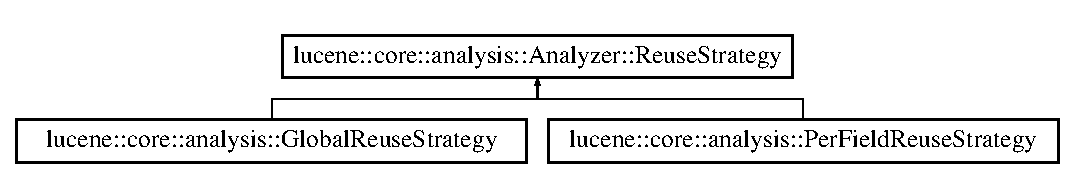
\includegraphics[height=1.951219cm]{classlucene_1_1core_1_1analysis_1_1Analyzer_1_1ReuseStrategy}
\end{center}
\end{figure}
\subsection*{Public Member Functions}
\begin{DoxyCompactItemize}
\item 
\mbox{\hyperlink{classlucene_1_1core_1_1analysis_1_1Analyzer_1_1ReuseStrategy_ac552252b82448b1e6012ff4024d99bfb}{Reuse\+Strategy}} ()
\item 
virtual \mbox{\hyperlink{classlucene_1_1core_1_1analysis_1_1Analyzer_1_1ReuseStrategy_ad113005e836ba6846d1fa2b6a1ae5924}{$\sim$\+Reuse\+Strategy}} ()
\item 
virtual \mbox{\hyperlink{classlucene_1_1core_1_1analysis_1_1TokenStreamComponents}{Token\+Stream\+Components}} $\ast$ \mbox{\hyperlink{classlucene_1_1core_1_1analysis_1_1Analyzer_1_1ReuseStrategy_ab180767950f392037e8ddf78c2f11f95}{Get\+Reusable\+Components}} (\mbox{\hyperlink{classlucene_1_1core_1_1analysis_1_1Analyzer}{Analyzer}} \&analyzer, \mbox{\hyperlink{ZlibCrc32_8h_a2c212835823e3c54a8ab6d95c652660e}{const}} std\+::string \&field\+\_\+name)=0
\item 
virtual void \mbox{\hyperlink{classlucene_1_1core_1_1analysis_1_1Analyzer_1_1ReuseStrategy_a78a1328d5564e78e2168169b73094b23}{Set\+Reusable\+Components}} (\mbox{\hyperlink{classlucene_1_1core_1_1analysis_1_1Analyzer}{Analyzer}} \&analyzer, \mbox{\hyperlink{ZlibCrc32_8h_a2c212835823e3c54a8ab6d95c652660e}{const}} std\+::string \&field\+\_\+name, \mbox{\hyperlink{classlucene_1_1core_1_1analysis_1_1TokenStreamComponents}{Token\+Stream\+Components}} $\ast$components)=0
\end{DoxyCompactItemize}


\subsection{Constructor \& Destructor Documentation}
\mbox{\Hypertarget{classlucene_1_1core_1_1analysis_1_1Analyzer_1_1ReuseStrategy_ac552252b82448b1e6012ff4024d99bfb}\label{classlucene_1_1core_1_1analysis_1_1Analyzer_1_1ReuseStrategy_ac552252b82448b1e6012ff4024d99bfb}} 
\index{lucene\+::core\+::analysis\+::\+Analyzer\+::\+Reuse\+Strategy@{lucene\+::core\+::analysis\+::\+Analyzer\+::\+Reuse\+Strategy}!Reuse\+Strategy@{Reuse\+Strategy}}
\index{Reuse\+Strategy@{Reuse\+Strategy}!lucene\+::core\+::analysis\+::\+Analyzer\+::\+Reuse\+Strategy@{lucene\+::core\+::analysis\+::\+Analyzer\+::\+Reuse\+Strategy}}
\subsubsection{\texorpdfstring{Reuse\+Strategy()}{ReuseStrategy()}}
{\footnotesize\ttfamily Analyzer\+::\+Reuse\+Strategy\+::\+Reuse\+Strategy (\begin{DoxyParamCaption}{ }\end{DoxyParamCaption})}

\mbox{\hyperlink{classlucene_1_1core_1_1analysis_1_1Analyzer_1_1ReuseStrategy}{Reuse\+Strategy}} \mbox{\Hypertarget{classlucene_1_1core_1_1analysis_1_1Analyzer_1_1ReuseStrategy_ad113005e836ba6846d1fa2b6a1ae5924}\label{classlucene_1_1core_1_1analysis_1_1Analyzer_1_1ReuseStrategy_ad113005e836ba6846d1fa2b6a1ae5924}} 
\index{lucene\+::core\+::analysis\+::\+Analyzer\+::\+Reuse\+Strategy@{lucene\+::core\+::analysis\+::\+Analyzer\+::\+Reuse\+Strategy}!````~Reuse\+Strategy@{$\sim$\+Reuse\+Strategy}}
\index{````~Reuse\+Strategy@{$\sim$\+Reuse\+Strategy}!lucene\+::core\+::analysis\+::\+Analyzer\+::\+Reuse\+Strategy@{lucene\+::core\+::analysis\+::\+Analyzer\+::\+Reuse\+Strategy}}
\subsubsection{\texorpdfstring{$\sim$\+Reuse\+Strategy()}{~ReuseStrategy()}}
{\footnotesize\ttfamily Analyzer\+::\+Reuse\+Strategy\+::$\sim$\+Reuse\+Strategy (\begin{DoxyParamCaption}{ }\end{DoxyParamCaption})\hspace{0.3cm}{\ttfamily [virtual]}}



\subsection{Member Function Documentation}
\mbox{\Hypertarget{classlucene_1_1core_1_1analysis_1_1Analyzer_1_1ReuseStrategy_ab180767950f392037e8ddf78c2f11f95}\label{classlucene_1_1core_1_1analysis_1_1Analyzer_1_1ReuseStrategy_ab180767950f392037e8ddf78c2f11f95}} 
\index{lucene\+::core\+::analysis\+::\+Analyzer\+::\+Reuse\+Strategy@{lucene\+::core\+::analysis\+::\+Analyzer\+::\+Reuse\+Strategy}!Get\+Reusable\+Components@{Get\+Reusable\+Components}}
\index{Get\+Reusable\+Components@{Get\+Reusable\+Components}!lucene\+::core\+::analysis\+::\+Analyzer\+::\+Reuse\+Strategy@{lucene\+::core\+::analysis\+::\+Analyzer\+::\+Reuse\+Strategy}}
\subsubsection{\texorpdfstring{Get\+Reusable\+Components()}{GetReusableComponents()}}
{\footnotesize\ttfamily virtual \mbox{\hyperlink{classlucene_1_1core_1_1analysis_1_1TokenStreamComponents}{Token\+Stream\+Components}}$\ast$ lucene\+::core\+::analysis\+::\+Analyzer\+::\+Reuse\+Strategy\+::\+Get\+Reusable\+Components (\begin{DoxyParamCaption}\item[{\mbox{\hyperlink{classlucene_1_1core_1_1analysis_1_1Analyzer}{Analyzer}} \&}]{analyzer,  }\item[{\mbox{\hyperlink{ZlibCrc32_8h_a2c212835823e3c54a8ab6d95c652660e}{const}} std\+::string \&}]{field\+\_\+name }\end{DoxyParamCaption})\hspace{0.3cm}{\ttfamily [pure virtual]}}



Implemented in \mbox{\hyperlink{classlucene_1_1core_1_1analysis_1_1PerFieldReuseStrategy_ab0d86155823842bb28e43bbbec7c06d3}{lucene\+::core\+::analysis\+::\+Per\+Field\+Reuse\+Strategy}}, and \mbox{\hyperlink{classlucene_1_1core_1_1analysis_1_1GlobalReuseStrategy_a79b31d1f8bf9bec685377f6dbff3c5ba}{lucene\+::core\+::analysis\+::\+Global\+Reuse\+Strategy}}.

\mbox{\Hypertarget{classlucene_1_1core_1_1analysis_1_1Analyzer_1_1ReuseStrategy_a78a1328d5564e78e2168169b73094b23}\label{classlucene_1_1core_1_1analysis_1_1Analyzer_1_1ReuseStrategy_a78a1328d5564e78e2168169b73094b23}} 
\index{lucene\+::core\+::analysis\+::\+Analyzer\+::\+Reuse\+Strategy@{lucene\+::core\+::analysis\+::\+Analyzer\+::\+Reuse\+Strategy}!Set\+Reusable\+Components@{Set\+Reusable\+Components}}
\index{Set\+Reusable\+Components@{Set\+Reusable\+Components}!lucene\+::core\+::analysis\+::\+Analyzer\+::\+Reuse\+Strategy@{lucene\+::core\+::analysis\+::\+Analyzer\+::\+Reuse\+Strategy}}
\subsubsection{\texorpdfstring{Set\+Reusable\+Components()}{SetReusableComponents()}}
{\footnotesize\ttfamily virtual void lucene\+::core\+::analysis\+::\+Analyzer\+::\+Reuse\+Strategy\+::\+Set\+Reusable\+Components (\begin{DoxyParamCaption}\item[{\mbox{\hyperlink{classlucene_1_1core_1_1analysis_1_1Analyzer}{Analyzer}} \&}]{analyzer,  }\item[{\mbox{\hyperlink{ZlibCrc32_8h_a2c212835823e3c54a8ab6d95c652660e}{const}} std\+::string \&}]{field\+\_\+name,  }\item[{\mbox{\hyperlink{classlucene_1_1core_1_1analysis_1_1TokenStreamComponents}{Token\+Stream\+Components}} $\ast$}]{components }\end{DoxyParamCaption})\hspace{0.3cm}{\ttfamily [pure virtual]}}



Implemented in \mbox{\hyperlink{classlucene_1_1core_1_1analysis_1_1PerFieldReuseStrategy_ab23b95640469c639fd36ac888eeda1c3}{lucene\+::core\+::analysis\+::\+Per\+Field\+Reuse\+Strategy}}, and \mbox{\hyperlink{classlucene_1_1core_1_1analysis_1_1GlobalReuseStrategy_a168d01df604559cb787781ad0ab7d7c2}{lucene\+::core\+::analysis\+::\+Global\+Reuse\+Strategy}}.



The documentation for this class was generated from the following files\+:\begin{DoxyCompactItemize}
\item 
Analysis/\mbox{\hyperlink{Analyzer_8h}{Analyzer.\+h}}\item 
Analysis/\mbox{\hyperlink{Analyzer_8cpp}{Analyzer.\+cpp}}\end{DoxyCompactItemize}

\hypertarget{classlucene_1_1core_1_1util_1_1Singleton}{}\section{lucene\+:\+:core\+:\+:util\+:\+:Singleton$<$ T\+Y\+PE $>$ Class Template Reference}
\label{classlucene_1_1core_1_1util_1_1Singleton}\index{lucene\+::core\+::util\+::\+Singleton$<$ T\+Y\+P\+E $>$@{lucene\+::core\+::util\+::\+Singleton$<$ T\+Y\+P\+E $>$}}


{\ttfamily \#include $<$Concurrency.\+h$>$}

\subsection*{Public Member Functions}
\begin{DoxyCompactItemize}
\item 
\mbox{\hyperlink{classlucene_1_1core_1_1util_1_1Singleton_ab5733f8687076b2ce608b096f91f5237}{Singleton}} (const \mbox{\hyperlink{classlucene_1_1core_1_1util_1_1Singleton}{Singleton}} \&)=delete
\item 
\mbox{\hyperlink{classlucene_1_1core_1_1util_1_1Singleton}{Singleton}} \& \mbox{\hyperlink{classlucene_1_1core_1_1util_1_1Singleton_abec7d88a0f754dfa66438cc76e4c5fd5}{operator=}} (const \mbox{\hyperlink{classlucene_1_1core_1_1util_1_1Singleton}{Singleton}} \&)=delete
\end{DoxyCompactItemize}
\subsection*{Static Public Member Functions}
\begin{DoxyCompactItemize}
\item 
static T\+Y\+PE \& \mbox{\hyperlink{classlucene_1_1core_1_1util_1_1Singleton_a5e8079ebbaae97438a52c449ee92aafa}{Get\+Instance}} ()
\end{DoxyCompactItemize}
\subsection*{Private Member Functions}
\begin{DoxyCompactItemize}
\item 
\mbox{\hyperlink{classlucene_1_1core_1_1util_1_1Singleton_a53448fc36821fec1c97716535987eaa7}{Singleton}} ()
\end{DoxyCompactItemize}


\subsection{Constructor \& Destructor Documentation}
\mbox{\Hypertarget{classlucene_1_1core_1_1util_1_1Singleton_a53448fc36821fec1c97716535987eaa7}\label{classlucene_1_1core_1_1util_1_1Singleton_a53448fc36821fec1c97716535987eaa7}} 
\index{lucene\+::core\+::util\+::\+Singleton@{lucene\+::core\+::util\+::\+Singleton}!Singleton@{Singleton}}
\index{Singleton@{Singleton}!lucene\+::core\+::util\+::\+Singleton@{lucene\+::core\+::util\+::\+Singleton}}
\subsubsection{\texorpdfstring{Singleton()}{Singleton()}\hspace{0.1cm}{\footnotesize\ttfamily [1/2]}}
{\footnotesize\ttfamily template$<$typename T\+Y\+PE $>$ \\
\mbox{\hyperlink{classlucene_1_1core_1_1util_1_1Singleton}{lucene\+::core\+::util\+::\+Singleton}}$<$ T\+Y\+PE $>$\+::\mbox{\hyperlink{classlucene_1_1core_1_1util_1_1Singleton}{Singleton}} (\begin{DoxyParamCaption}{ }\end{DoxyParamCaption})\hspace{0.3cm}{\ttfamily [inline]}, {\ttfamily [private]}}

\mbox{\Hypertarget{classlucene_1_1core_1_1util_1_1Singleton_ab5733f8687076b2ce608b096f91f5237}\label{classlucene_1_1core_1_1util_1_1Singleton_ab5733f8687076b2ce608b096f91f5237}} 
\index{lucene\+::core\+::util\+::\+Singleton@{lucene\+::core\+::util\+::\+Singleton}!Singleton@{Singleton}}
\index{Singleton@{Singleton}!lucene\+::core\+::util\+::\+Singleton@{lucene\+::core\+::util\+::\+Singleton}}
\subsubsection{\texorpdfstring{Singleton()}{Singleton()}\hspace{0.1cm}{\footnotesize\ttfamily [2/2]}}
{\footnotesize\ttfamily template$<$typename T\+Y\+PE $>$ \\
\mbox{\hyperlink{classlucene_1_1core_1_1util_1_1Singleton}{lucene\+::core\+::util\+::\+Singleton}}$<$ T\+Y\+PE $>$\+::\mbox{\hyperlink{classlucene_1_1core_1_1util_1_1Singleton}{Singleton}} (\begin{DoxyParamCaption}\item[{const \mbox{\hyperlink{classlucene_1_1core_1_1util_1_1Singleton}{Singleton}}$<$ T\+Y\+PE $>$ \&}]{ }\end{DoxyParamCaption})\hspace{0.3cm}{\ttfamily [delete]}}



\subsection{Member Function Documentation}
\mbox{\Hypertarget{classlucene_1_1core_1_1util_1_1Singleton_a5e8079ebbaae97438a52c449ee92aafa}\label{classlucene_1_1core_1_1util_1_1Singleton_a5e8079ebbaae97438a52c449ee92aafa}} 
\index{lucene\+::core\+::util\+::\+Singleton@{lucene\+::core\+::util\+::\+Singleton}!Get\+Instance@{Get\+Instance}}
\index{Get\+Instance@{Get\+Instance}!lucene\+::core\+::util\+::\+Singleton@{lucene\+::core\+::util\+::\+Singleton}}
\subsubsection{\texorpdfstring{Get\+Instance()}{GetInstance()}}
{\footnotesize\ttfamily template$<$typename T\+Y\+PE $>$ \\
static T\+Y\+PE\& \mbox{\hyperlink{classlucene_1_1core_1_1util_1_1Singleton}{lucene\+::core\+::util\+::\+Singleton}}$<$ T\+Y\+PE $>$\+::Get\+Instance (\begin{DoxyParamCaption}{ }\end{DoxyParamCaption})\hspace{0.3cm}{\ttfamily [inline]}, {\ttfamily [static]}}

\mbox{\Hypertarget{classlucene_1_1core_1_1util_1_1Singleton_abec7d88a0f754dfa66438cc76e4c5fd5}\label{classlucene_1_1core_1_1util_1_1Singleton_abec7d88a0f754dfa66438cc76e4c5fd5}} 
\index{lucene\+::core\+::util\+::\+Singleton@{lucene\+::core\+::util\+::\+Singleton}!operator=@{operator=}}
\index{operator=@{operator=}!lucene\+::core\+::util\+::\+Singleton@{lucene\+::core\+::util\+::\+Singleton}}
\subsubsection{\texorpdfstring{operator=()}{operator=()}}
{\footnotesize\ttfamily template$<$typename T\+Y\+PE $>$ \\
\mbox{\hyperlink{classlucene_1_1core_1_1util_1_1Singleton}{Singleton}}\& \mbox{\hyperlink{classlucene_1_1core_1_1util_1_1Singleton}{lucene\+::core\+::util\+::\+Singleton}}$<$ T\+Y\+PE $>$\+::operator= (\begin{DoxyParamCaption}\item[{const \mbox{\hyperlink{classlucene_1_1core_1_1util_1_1Singleton}{Singleton}}$<$ T\+Y\+PE $>$ \&}]{ }\end{DoxyParamCaption})\hspace{0.3cm}{\ttfamily [delete]}}



The documentation for this class was generated from the following file\+:\begin{DoxyCompactItemize}
\item 
Util/\mbox{\hyperlink{Concurrency_8h}{Concurrency.\+h}}\end{DoxyCompactItemize}

\hypertarget{classlucene_1_1core_1_1analysis_1_1standard_1_1StandardAnalyzer}{}\section{lucene\+:\+:core\+:\+:analysis\+:\+:standard\+:\+:Standard\+Analyzer Class Reference}
\label{classlucene_1_1core_1_1analysis_1_1standard_1_1StandardAnalyzer}\index{lucene\+::core\+::analysis\+::standard\+::\+Standard\+Analyzer@{lucene\+::core\+::analysis\+::standard\+::\+Standard\+Analyzer}}


{\ttfamily \#include $<$Standard.\+h$>$}

Inheritance diagram for lucene\+:\+:core\+:\+:analysis\+:\+:standard\+:\+:Standard\+Analyzer\+:\begin{figure}[H]
\begin{center}
\leavevmode
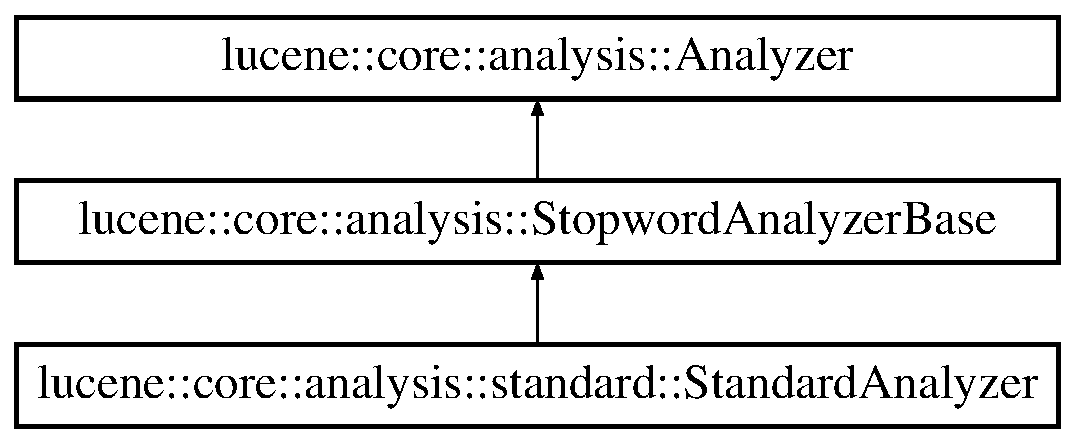
\includegraphics[height=3.000000cm]{classlucene_1_1core_1_1analysis_1_1standard_1_1StandardAnalyzer}
\end{center}
\end{figure}
\subsection*{Public Member Functions}
\begin{DoxyCompactItemize}
\item 
\mbox{\hyperlink{classlucene_1_1core_1_1analysis_1_1standard_1_1StandardAnalyzer_a96aade9f9e04262af76d6f69d5ba3103}{Standard\+Analyzer}} ()
\item 
\mbox{\hyperlink{classlucene_1_1core_1_1analysis_1_1standard_1_1StandardAnalyzer_afe3086be0798a7a38675170d12ef0d31}{Standard\+Analyzer}} (\mbox{\hyperlink{classlucene_1_1core_1_1analysis_1_1Reader}{lucene\+::core\+::analysis\+::\+Reader}} \&\&\mbox{\hyperlink{classlucene_1_1core_1_1analysis_1_1StopwordAnalyzerBase_a12ceda198e84aabe357ccd7b28e66d07}{stop\+\_\+words}})
\item 
\mbox{\hyperlink{classlucene_1_1core_1_1analysis_1_1standard_1_1StandardAnalyzer_a50b9c11d1c78184c0518fbf19c6486ce}{Standard\+Analyzer}} (\mbox{\hyperlink{ZlibCrc32_8h_a2c212835823e3c54a8ab6d95c652660e}{const}} \mbox{\hyperlink{classlucene_1_1core_1_1analysis_1_1characterutil_1_1CharSet}{lucene\+::core\+::analysis\+::characterutil\+::\+Char\+Set}} \&\mbox{\hyperlink{classlucene_1_1core_1_1analysis_1_1StopwordAnalyzerBase_a12ceda198e84aabe357ccd7b28e66d07}{stop\+\_\+words}})
\item 
\mbox{\hyperlink{classlucene_1_1core_1_1analysis_1_1standard_1_1StandardAnalyzer_acc4853fc9cc1c394d9d0e8b5d0d98796}{Standard\+Analyzer}} (\mbox{\hyperlink{classlucene_1_1core_1_1analysis_1_1characterutil_1_1CharSet}{lucene\+::core\+::analysis\+::characterutil\+::\+Char\+Set}} \&\&\mbox{\hyperlink{classlucene_1_1core_1_1analysis_1_1StopwordAnalyzerBase_a12ceda198e84aabe357ccd7b28e66d07}{stop\+\_\+words}})
\item 
\mbox{\hyperlink{classlucene_1_1core_1_1analysis_1_1standard_1_1StandardAnalyzer_a241082c932a211751c3d437886d50ba0}{$\sim$\+Standard\+Analyzer}} ()
\item 
void \mbox{\hyperlink{classlucene_1_1core_1_1analysis_1_1standard_1_1StandardAnalyzer_af00b69646ec366ab9319197824f12e4b}{Set\+Max\+Token\+Length}} (\mbox{\hyperlink{ZlibCrc32_8h_a2c212835823e3c54a8ab6d95c652660e}{const}} uint32\+\_\+t length)
\item 
uint32\+\_\+t \mbox{\hyperlink{classlucene_1_1core_1_1analysis_1_1standard_1_1StandardAnalyzer_a383601d5fa0bcd3883f794c887512517}{Get\+Max\+Token\+Length}} ()
\end{DoxyCompactItemize}
\subsection*{Static Public Attributes}
\begin{DoxyCompactItemize}
\item 
static \mbox{\hyperlink{ZlibCrc32_8h_a2c212835823e3c54a8ab6d95c652660e}{const}} uint32\+\_\+t \mbox{\hyperlink{classlucene_1_1core_1_1analysis_1_1standard_1_1StandardAnalyzer_a3c01017747853f232cdceee30fea7a35}{D\+E\+F\+A\+U\+L\+T\+\_\+\+M\+A\+X\+\_\+\+T\+O\+K\+E\+N\+\_\+\+L\+E\+N\+G\+TH}} = 255
\item 
static \mbox{\hyperlink{ZlibCrc32_8h_a2c212835823e3c54a8ab6d95c652660e}{const}} \mbox{\hyperlink{classlucene_1_1core_1_1analysis_1_1characterutil_1_1CharSet}{lucene\+::core\+::analysis\+::characterutil\+::\+Char\+Set}} \mbox{\hyperlink{classlucene_1_1core_1_1analysis_1_1standard_1_1StandardAnalyzer_a43ca4db920b102be1fd2d7c2191fc69e}{S\+T\+O\+P\+\_\+\+W\+O\+R\+D\+S\+\_\+\+S\+ET}}
\end{DoxyCompactItemize}
\subsection*{Protected Member Functions}
\begin{DoxyCompactItemize}
\item 
\mbox{\hyperlink{classlucene_1_1core_1_1analysis_1_1TokenStreamComponents}{Token\+Stream\+Components}} $\ast$ \mbox{\hyperlink{classlucene_1_1core_1_1analysis_1_1standard_1_1StandardAnalyzer_a0d569e3e48f2060a4698481ec1b49d12}{Create\+Components}} (\mbox{\hyperlink{ZlibCrc32_8h_a2c212835823e3c54a8ab6d95c652660e}{const}} std\+::string \&field\+\_\+name) override
\item 
\mbox{\hyperlink{namespacelucene_1_1core_1_1analysis_a1ecb3e92b19c3afd8060d81a437a7a3b}{delete\+\_\+unique\+\_\+ptr}}$<$ \mbox{\hyperlink{classlucene_1_1core_1_1analysis_1_1TokenStream}{Token\+Stream}} $>$ \mbox{\hyperlink{classlucene_1_1core_1_1analysis_1_1standard_1_1StandardAnalyzer_aa42382c6504229a195abbc25f048a614}{Normalize}} (\mbox{\hyperlink{ZlibCrc32_8h_a2c212835823e3c54a8ab6d95c652660e}{const}} std\+::string \&field\+\_\+name, \mbox{\hyperlink{namespacelucene_1_1core_1_1analysis_a1ecb3e92b19c3afd8060d81a437a7a3b}{delete\+\_\+unique\+\_\+ptr}}$<$ \mbox{\hyperlink{classlucene_1_1core_1_1analysis_1_1TokenStream}{Token\+Stream}} $>$ in)
\end{DoxyCompactItemize}
\subsection*{Private Attributes}
\begin{DoxyCompactItemize}
\item 
uint32\+\_\+t \mbox{\hyperlink{classlucene_1_1core_1_1analysis_1_1standard_1_1StandardAnalyzer_a3f094c0fd3d5efa0c8982e7bee81bbef}{max\+\_\+token\+\_\+length}}
\end{DoxyCompactItemize}
\subsection*{Additional Inherited Members}


\subsection{Constructor \& Destructor Documentation}
\mbox{\Hypertarget{classlucene_1_1core_1_1analysis_1_1standard_1_1StandardAnalyzer_a96aade9f9e04262af76d6f69d5ba3103}\label{classlucene_1_1core_1_1analysis_1_1standard_1_1StandardAnalyzer_a96aade9f9e04262af76d6f69d5ba3103}} 
\index{lucene\+::core\+::analysis\+::standard\+::\+Standard\+Analyzer@{lucene\+::core\+::analysis\+::standard\+::\+Standard\+Analyzer}!Standard\+Analyzer@{Standard\+Analyzer}}
\index{Standard\+Analyzer@{Standard\+Analyzer}!lucene\+::core\+::analysis\+::standard\+::\+Standard\+Analyzer@{lucene\+::core\+::analysis\+::standard\+::\+Standard\+Analyzer}}
\subsubsection{\texorpdfstring{Standard\+Analyzer()}{StandardAnalyzer()}\hspace{0.1cm}{\footnotesize\ttfamily [1/4]}}
{\footnotesize\ttfamily Standard\+Analyzer\+::\+Standard\+Analyzer (\begin{DoxyParamCaption}{ }\end{DoxyParamCaption})}

\mbox{\Hypertarget{classlucene_1_1core_1_1analysis_1_1standard_1_1StandardAnalyzer_afe3086be0798a7a38675170d12ef0d31}\label{classlucene_1_1core_1_1analysis_1_1standard_1_1StandardAnalyzer_afe3086be0798a7a38675170d12ef0d31}} 
\index{lucene\+::core\+::analysis\+::standard\+::\+Standard\+Analyzer@{lucene\+::core\+::analysis\+::standard\+::\+Standard\+Analyzer}!Standard\+Analyzer@{Standard\+Analyzer}}
\index{Standard\+Analyzer@{Standard\+Analyzer}!lucene\+::core\+::analysis\+::standard\+::\+Standard\+Analyzer@{lucene\+::core\+::analysis\+::standard\+::\+Standard\+Analyzer}}
\subsubsection{\texorpdfstring{Standard\+Analyzer()}{StandardAnalyzer()}\hspace{0.1cm}{\footnotesize\ttfamily [2/4]}}
{\footnotesize\ttfamily lucene\+::core\+::analysis\+::standard\+::\+Standard\+Analyzer\+::\+Standard\+Analyzer (\begin{DoxyParamCaption}\item[{\mbox{\hyperlink{classlucene_1_1core_1_1analysis_1_1Reader}{lucene\+::core\+::analysis\+::\+Reader}} \&\&}]{stop\+\_\+words }\end{DoxyParamCaption})\hspace{0.3cm}{\ttfamily [explicit]}}

\mbox{\Hypertarget{classlucene_1_1core_1_1analysis_1_1standard_1_1StandardAnalyzer_a50b9c11d1c78184c0518fbf19c6486ce}\label{classlucene_1_1core_1_1analysis_1_1standard_1_1StandardAnalyzer_a50b9c11d1c78184c0518fbf19c6486ce}} 
\index{lucene\+::core\+::analysis\+::standard\+::\+Standard\+Analyzer@{lucene\+::core\+::analysis\+::standard\+::\+Standard\+Analyzer}!Standard\+Analyzer@{Standard\+Analyzer}}
\index{Standard\+Analyzer@{Standard\+Analyzer}!lucene\+::core\+::analysis\+::standard\+::\+Standard\+Analyzer@{lucene\+::core\+::analysis\+::standard\+::\+Standard\+Analyzer}}
\subsubsection{\texorpdfstring{Standard\+Analyzer()}{StandardAnalyzer()}\hspace{0.1cm}{\footnotesize\ttfamily [3/4]}}
{\footnotesize\ttfamily Standard\+Analyzer\+::\+Standard\+Analyzer (\begin{DoxyParamCaption}\item[{\mbox{\hyperlink{ZlibCrc32_8h_a2c212835823e3c54a8ab6d95c652660e}{const}} \mbox{\hyperlink{classlucene_1_1core_1_1analysis_1_1characterutil_1_1CharSet}{lucene\+::core\+::analysis\+::characterutil\+::\+Char\+Set}} \&}]{stop\+\_\+words }\end{DoxyParamCaption})}

\mbox{\Hypertarget{classlucene_1_1core_1_1analysis_1_1standard_1_1StandardAnalyzer_acc4853fc9cc1c394d9d0e8b5d0d98796}\label{classlucene_1_1core_1_1analysis_1_1standard_1_1StandardAnalyzer_acc4853fc9cc1c394d9d0e8b5d0d98796}} 
\index{lucene\+::core\+::analysis\+::standard\+::\+Standard\+Analyzer@{lucene\+::core\+::analysis\+::standard\+::\+Standard\+Analyzer}!Standard\+Analyzer@{Standard\+Analyzer}}
\index{Standard\+Analyzer@{Standard\+Analyzer}!lucene\+::core\+::analysis\+::standard\+::\+Standard\+Analyzer@{lucene\+::core\+::analysis\+::standard\+::\+Standard\+Analyzer}}
\subsubsection{\texorpdfstring{Standard\+Analyzer()}{StandardAnalyzer()}\hspace{0.1cm}{\footnotesize\ttfamily [4/4]}}
{\footnotesize\ttfamily Standard\+Analyzer\+::\+Standard\+Analyzer (\begin{DoxyParamCaption}\item[{\mbox{\hyperlink{classlucene_1_1core_1_1analysis_1_1characterutil_1_1CharSet}{lucene\+::core\+::analysis\+::characterutil\+::\+Char\+Set}} \&\&}]{stop\+\_\+words }\end{DoxyParamCaption})\hspace{0.3cm}{\ttfamily [explicit]}}

\mbox{\Hypertarget{classlucene_1_1core_1_1analysis_1_1standard_1_1StandardAnalyzer_a241082c932a211751c3d437886d50ba0}\label{classlucene_1_1core_1_1analysis_1_1standard_1_1StandardAnalyzer_a241082c932a211751c3d437886d50ba0}} 
\index{lucene\+::core\+::analysis\+::standard\+::\+Standard\+Analyzer@{lucene\+::core\+::analysis\+::standard\+::\+Standard\+Analyzer}!````~Standard\+Analyzer@{$\sim$\+Standard\+Analyzer}}
\index{````~Standard\+Analyzer@{$\sim$\+Standard\+Analyzer}!lucene\+::core\+::analysis\+::standard\+::\+Standard\+Analyzer@{lucene\+::core\+::analysis\+::standard\+::\+Standard\+Analyzer}}
\subsubsection{\texorpdfstring{$\sim$\+Standard\+Analyzer()}{~StandardAnalyzer()}}
{\footnotesize\ttfamily Standard\+Analyzer\+::$\sim$\+Standard\+Analyzer (\begin{DoxyParamCaption}{ }\end{DoxyParamCaption})}



\subsection{Member Function Documentation}
\mbox{\Hypertarget{classlucene_1_1core_1_1analysis_1_1standard_1_1StandardAnalyzer_a0d569e3e48f2060a4698481ec1b49d12}\label{classlucene_1_1core_1_1analysis_1_1standard_1_1StandardAnalyzer_a0d569e3e48f2060a4698481ec1b49d12}} 
\index{lucene\+::core\+::analysis\+::standard\+::\+Standard\+Analyzer@{lucene\+::core\+::analysis\+::standard\+::\+Standard\+Analyzer}!Create\+Components@{Create\+Components}}
\index{Create\+Components@{Create\+Components}!lucene\+::core\+::analysis\+::standard\+::\+Standard\+Analyzer@{lucene\+::core\+::analysis\+::standard\+::\+Standard\+Analyzer}}
\subsubsection{\texorpdfstring{Create\+Components()}{CreateComponents()}}
{\footnotesize\ttfamily \mbox{\hyperlink{classlucene_1_1core_1_1analysis_1_1TokenStreamComponents}{Token\+Stream\+Components}} $\ast$ Standard\+Analyzer\+::\+Create\+Components (\begin{DoxyParamCaption}\item[{\mbox{\hyperlink{ZlibCrc32_8h_a2c212835823e3c54a8ab6d95c652660e}{const}} std\+::string \&}]{field\+\_\+name }\end{DoxyParamCaption})\hspace{0.3cm}{\ttfamily [override]}, {\ttfamily [protected]}, {\ttfamily [virtual]}}



Implements \mbox{\hyperlink{classlucene_1_1core_1_1analysis_1_1Analyzer_a9b7dc3c598057fbf4e9b5f48066cb54a}{lucene\+::core\+::analysis\+::\+Analyzer}}.

\mbox{\Hypertarget{classlucene_1_1core_1_1analysis_1_1standard_1_1StandardAnalyzer_a383601d5fa0bcd3883f794c887512517}\label{classlucene_1_1core_1_1analysis_1_1standard_1_1StandardAnalyzer_a383601d5fa0bcd3883f794c887512517}} 
\index{lucene\+::core\+::analysis\+::standard\+::\+Standard\+Analyzer@{lucene\+::core\+::analysis\+::standard\+::\+Standard\+Analyzer}!Get\+Max\+Token\+Length@{Get\+Max\+Token\+Length}}
\index{Get\+Max\+Token\+Length@{Get\+Max\+Token\+Length}!lucene\+::core\+::analysis\+::standard\+::\+Standard\+Analyzer@{lucene\+::core\+::analysis\+::standard\+::\+Standard\+Analyzer}}
\subsubsection{\texorpdfstring{Get\+Max\+Token\+Length()}{GetMaxTokenLength()}}
{\footnotesize\ttfamily uint32\+\_\+t Standard\+Analyzer\+::\+Get\+Max\+Token\+Length (\begin{DoxyParamCaption}{ }\end{DoxyParamCaption})}

\mbox{\Hypertarget{classlucene_1_1core_1_1analysis_1_1standard_1_1StandardAnalyzer_aa42382c6504229a195abbc25f048a614}\label{classlucene_1_1core_1_1analysis_1_1standard_1_1StandardAnalyzer_aa42382c6504229a195abbc25f048a614}} 
\index{lucene\+::core\+::analysis\+::standard\+::\+Standard\+Analyzer@{lucene\+::core\+::analysis\+::standard\+::\+Standard\+Analyzer}!Normalize@{Normalize}}
\index{Normalize@{Normalize}!lucene\+::core\+::analysis\+::standard\+::\+Standard\+Analyzer@{lucene\+::core\+::analysis\+::standard\+::\+Standard\+Analyzer}}
\subsubsection{\texorpdfstring{Normalize()}{Normalize()}}
{\footnotesize\ttfamily \mbox{\hyperlink{namespacelucene_1_1core_1_1analysis_a1ecb3e92b19c3afd8060d81a437a7a3b}{delete\+\_\+unique\+\_\+ptr}}$<$ \mbox{\hyperlink{classlucene_1_1core_1_1analysis_1_1TokenStream}{Token\+Stream}} $>$ Standard\+Analyzer\+::\+Normalize (\begin{DoxyParamCaption}\item[{\mbox{\hyperlink{ZlibCrc32_8h_a2c212835823e3c54a8ab6d95c652660e}{const}} std\+::string \&}]{field\+\_\+name,  }\item[{\mbox{\hyperlink{namespacelucene_1_1core_1_1analysis_a1ecb3e92b19c3afd8060d81a437a7a3b}{delete\+\_\+unique\+\_\+ptr}}$<$ \mbox{\hyperlink{classlucene_1_1core_1_1analysis_1_1TokenStream}{Token\+Stream}} $>$}]{in }\end{DoxyParamCaption})\hspace{0.3cm}{\ttfamily [protected]}}

\mbox{\Hypertarget{classlucene_1_1core_1_1analysis_1_1standard_1_1StandardAnalyzer_af00b69646ec366ab9319197824f12e4b}\label{classlucene_1_1core_1_1analysis_1_1standard_1_1StandardAnalyzer_af00b69646ec366ab9319197824f12e4b}} 
\index{lucene\+::core\+::analysis\+::standard\+::\+Standard\+Analyzer@{lucene\+::core\+::analysis\+::standard\+::\+Standard\+Analyzer}!Set\+Max\+Token\+Length@{Set\+Max\+Token\+Length}}
\index{Set\+Max\+Token\+Length@{Set\+Max\+Token\+Length}!lucene\+::core\+::analysis\+::standard\+::\+Standard\+Analyzer@{lucene\+::core\+::analysis\+::standard\+::\+Standard\+Analyzer}}
\subsubsection{\texorpdfstring{Set\+Max\+Token\+Length()}{SetMaxTokenLength()}}
{\footnotesize\ttfamily void Standard\+Analyzer\+::\+Set\+Max\+Token\+Length (\begin{DoxyParamCaption}\item[{\mbox{\hyperlink{ZlibCrc32_8h_a2c212835823e3c54a8ab6d95c652660e}{const}} uint32\+\_\+t}]{length }\end{DoxyParamCaption})}



\subsection{Member Data Documentation}
\mbox{\Hypertarget{classlucene_1_1core_1_1analysis_1_1standard_1_1StandardAnalyzer_a3c01017747853f232cdceee30fea7a35}\label{classlucene_1_1core_1_1analysis_1_1standard_1_1StandardAnalyzer_a3c01017747853f232cdceee30fea7a35}} 
\index{lucene\+::core\+::analysis\+::standard\+::\+Standard\+Analyzer@{lucene\+::core\+::analysis\+::standard\+::\+Standard\+Analyzer}!D\+E\+F\+A\+U\+L\+T\+\_\+\+M\+A\+X\+\_\+\+T\+O\+K\+E\+N\+\_\+\+L\+E\+N\+G\+TH@{D\+E\+F\+A\+U\+L\+T\+\_\+\+M\+A\+X\+\_\+\+T\+O\+K\+E\+N\+\_\+\+L\+E\+N\+G\+TH}}
\index{D\+E\+F\+A\+U\+L\+T\+\_\+\+M\+A\+X\+\_\+\+T\+O\+K\+E\+N\+\_\+\+L\+E\+N\+G\+TH@{D\+E\+F\+A\+U\+L\+T\+\_\+\+M\+A\+X\+\_\+\+T\+O\+K\+E\+N\+\_\+\+L\+E\+N\+G\+TH}!lucene\+::core\+::analysis\+::standard\+::\+Standard\+Analyzer@{lucene\+::core\+::analysis\+::standard\+::\+Standard\+Analyzer}}
\subsubsection{\texorpdfstring{D\+E\+F\+A\+U\+L\+T\+\_\+\+M\+A\+X\+\_\+\+T\+O\+K\+E\+N\+\_\+\+L\+E\+N\+G\+TH}{DEFAULT\_MAX\_TOKEN\_LENGTH}}
{\footnotesize\ttfamily \mbox{\hyperlink{ZlibCrc32_8h_a2c212835823e3c54a8ab6d95c652660e}{const}} uint32\+\_\+t lucene\+::core\+::analysis\+::standard\+::\+Standard\+Analyzer\+::\+D\+E\+F\+A\+U\+L\+T\+\_\+\+M\+A\+X\+\_\+\+T\+O\+K\+E\+N\+\_\+\+L\+E\+N\+G\+TH = 255\hspace{0.3cm}{\ttfamily [static]}}

\mbox{\Hypertarget{classlucene_1_1core_1_1analysis_1_1standard_1_1StandardAnalyzer_a3f094c0fd3d5efa0c8982e7bee81bbef}\label{classlucene_1_1core_1_1analysis_1_1standard_1_1StandardAnalyzer_a3f094c0fd3d5efa0c8982e7bee81bbef}} 
\index{lucene\+::core\+::analysis\+::standard\+::\+Standard\+Analyzer@{lucene\+::core\+::analysis\+::standard\+::\+Standard\+Analyzer}!max\+\_\+token\+\_\+length@{max\+\_\+token\+\_\+length}}
\index{max\+\_\+token\+\_\+length@{max\+\_\+token\+\_\+length}!lucene\+::core\+::analysis\+::standard\+::\+Standard\+Analyzer@{lucene\+::core\+::analysis\+::standard\+::\+Standard\+Analyzer}}
\subsubsection{\texorpdfstring{max\+\_\+token\+\_\+length}{max\_token\_length}}
{\footnotesize\ttfamily uint32\+\_\+t lucene\+::core\+::analysis\+::standard\+::\+Standard\+Analyzer\+::max\+\_\+token\+\_\+length\hspace{0.3cm}{\ttfamily [private]}}

\mbox{\Hypertarget{classlucene_1_1core_1_1analysis_1_1standard_1_1StandardAnalyzer_a43ca4db920b102be1fd2d7c2191fc69e}\label{classlucene_1_1core_1_1analysis_1_1standard_1_1StandardAnalyzer_a43ca4db920b102be1fd2d7c2191fc69e}} 
\index{lucene\+::core\+::analysis\+::standard\+::\+Standard\+Analyzer@{lucene\+::core\+::analysis\+::standard\+::\+Standard\+Analyzer}!S\+T\+O\+P\+\_\+\+W\+O\+R\+D\+S\+\_\+\+S\+ET@{S\+T\+O\+P\+\_\+\+W\+O\+R\+D\+S\+\_\+\+S\+ET}}
\index{S\+T\+O\+P\+\_\+\+W\+O\+R\+D\+S\+\_\+\+S\+ET@{S\+T\+O\+P\+\_\+\+W\+O\+R\+D\+S\+\_\+\+S\+ET}!lucene\+::core\+::analysis\+::standard\+::\+Standard\+Analyzer@{lucene\+::core\+::analysis\+::standard\+::\+Standard\+Analyzer}}
\subsubsection{\texorpdfstring{S\+T\+O\+P\+\_\+\+W\+O\+R\+D\+S\+\_\+\+S\+ET}{STOP\_WORDS\_SET}}
{\footnotesize\ttfamily \mbox{\hyperlink{ZlibCrc32_8h_a2c212835823e3c54a8ab6d95c652660e}{const}} Char\+Set Standard\+Analyzer\+::\+S\+T\+O\+P\+\_\+\+W\+O\+R\+D\+S\+\_\+\+S\+ET\hspace{0.3cm}{\ttfamily [static]}}



The documentation for this class was generated from the following files\+:\begin{DoxyCompactItemize}
\item 
Analysis/\mbox{\hyperlink{Standard_8h}{Standard.\+h}}\item 
Analysis/\mbox{\hyperlink{Standard_8cpp}{Standard.\+cpp}}\end{DoxyCompactItemize}

\hypertarget{classlucene_1_1core_1_1analysis_1_1standard_1_1StandardFilter}{}\section{lucene\+:\+:core\+:\+:analysis\+:\+:standard\+:\+:Standard\+Filter Class Reference}
\label{classlucene_1_1core_1_1analysis_1_1standard_1_1StandardFilter}\index{lucene\+::core\+::analysis\+::standard\+::\+Standard\+Filter@{lucene\+::core\+::analysis\+::standard\+::\+Standard\+Filter}}


{\ttfamily \#include $<$Standard.\+h$>$}

Inheritance diagram for lucene\+:\+:core\+:\+:analysis\+:\+:standard\+:\+:Standard\+Filter\+:\begin{figure}[H]
\begin{center}
\leavevmode
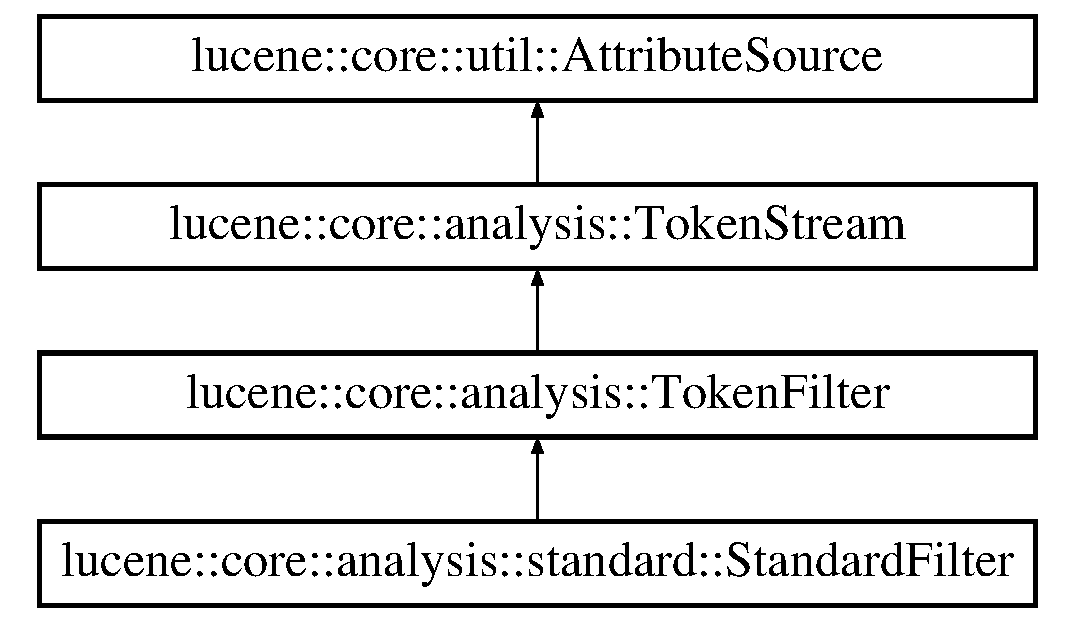
\includegraphics[height=4.000000cm]{classlucene_1_1core_1_1analysis_1_1standard_1_1StandardFilter}
\end{center}
\end{figure}
\subsection*{Public Member Functions}
\begin{DoxyCompactItemize}
\item 
\mbox{\hyperlink{classlucene_1_1core_1_1analysis_1_1standard_1_1StandardFilter_a2463bf01ed63b31b0df14149737e50ae}{Standard\+Filter}} (\mbox{\hyperlink{classlucene_1_1core_1_1analysis_1_1TokenStream}{Token\+Stream}} $\ast$in)
\item 
virtual \mbox{\hyperlink{classlucene_1_1core_1_1analysis_1_1standard_1_1StandardFilter_a0136fab7677e7393491b4075a852751d}{$\sim$\+Standard\+Filter}} ()
\item 
bool \mbox{\hyperlink{classlucene_1_1core_1_1analysis_1_1standard_1_1StandardFilter_a11958d89cb4aed281d083db7be0e8680}{Increment\+Token}} () override
\end{DoxyCompactItemize}
\subsection*{Additional Inherited Members}


\subsection{Constructor \& Destructor Documentation}
\mbox{\Hypertarget{classlucene_1_1core_1_1analysis_1_1standard_1_1StandardFilter_a2463bf01ed63b31b0df14149737e50ae}\label{classlucene_1_1core_1_1analysis_1_1standard_1_1StandardFilter_a2463bf01ed63b31b0df14149737e50ae}} 
\index{lucene\+::core\+::analysis\+::standard\+::\+Standard\+Filter@{lucene\+::core\+::analysis\+::standard\+::\+Standard\+Filter}!Standard\+Filter@{Standard\+Filter}}
\index{Standard\+Filter@{Standard\+Filter}!lucene\+::core\+::analysis\+::standard\+::\+Standard\+Filter@{lucene\+::core\+::analysis\+::standard\+::\+Standard\+Filter}}
\subsubsection{\texorpdfstring{Standard\+Filter()}{StandardFilter()}}
{\footnotesize\ttfamily Standard\+Filter\+::\+Standard\+Filter (\begin{DoxyParamCaption}\item[{\mbox{\hyperlink{classlucene_1_1core_1_1analysis_1_1TokenStream}{Token\+Stream}} $\ast$}]{in }\end{DoxyParamCaption})\hspace{0.3cm}{\ttfamily [explicit]}}

\mbox{\Hypertarget{classlucene_1_1core_1_1analysis_1_1standard_1_1StandardFilter_a0136fab7677e7393491b4075a852751d}\label{classlucene_1_1core_1_1analysis_1_1standard_1_1StandardFilter_a0136fab7677e7393491b4075a852751d}} 
\index{lucene\+::core\+::analysis\+::standard\+::\+Standard\+Filter@{lucene\+::core\+::analysis\+::standard\+::\+Standard\+Filter}!````~Standard\+Filter@{$\sim$\+Standard\+Filter}}
\index{````~Standard\+Filter@{$\sim$\+Standard\+Filter}!lucene\+::core\+::analysis\+::standard\+::\+Standard\+Filter@{lucene\+::core\+::analysis\+::standard\+::\+Standard\+Filter}}
\subsubsection{\texorpdfstring{$\sim$\+Standard\+Filter()}{~StandardFilter()}}
{\footnotesize\ttfamily Standard\+Filter\+::$\sim$\+Standard\+Filter (\begin{DoxyParamCaption}{ }\end{DoxyParamCaption})\hspace{0.3cm}{\ttfamily [virtual]}}



\subsection{Member Function Documentation}
\mbox{\Hypertarget{classlucene_1_1core_1_1analysis_1_1standard_1_1StandardFilter_a11958d89cb4aed281d083db7be0e8680}\label{classlucene_1_1core_1_1analysis_1_1standard_1_1StandardFilter_a11958d89cb4aed281d083db7be0e8680}} 
\index{lucene\+::core\+::analysis\+::standard\+::\+Standard\+Filter@{lucene\+::core\+::analysis\+::standard\+::\+Standard\+Filter}!Increment\+Token@{Increment\+Token}}
\index{Increment\+Token@{Increment\+Token}!lucene\+::core\+::analysis\+::standard\+::\+Standard\+Filter@{lucene\+::core\+::analysis\+::standard\+::\+Standard\+Filter}}
\subsubsection{\texorpdfstring{Increment\+Token()}{IncrementToken()}}
{\footnotesize\ttfamily bool Standard\+Filter\+::\+Increment\+Token (\begin{DoxyParamCaption}{ }\end{DoxyParamCaption})\hspace{0.3cm}{\ttfamily [override]}, {\ttfamily [virtual]}}



Implements \mbox{\hyperlink{classlucene_1_1core_1_1analysis_1_1TokenStream_a614d4ea24a354d6f4354b4941b5124e2}{lucene\+::core\+::analysis\+::\+Token\+Stream}}.



The documentation for this class was generated from the following files\+:\begin{DoxyCompactItemize}
\item 
Analysis/\mbox{\hyperlink{Standard_8h}{Standard.\+h}}\item 
Analysis/\mbox{\hyperlink{Standard_8cpp}{Standard.\+cpp}}\end{DoxyCompactItemize}

\hypertarget{classlucene_1_1core_1_1analysis_1_1standard_1_1StandardTokenizer}{}\section{lucene\+:\+:core\+:\+:analysis\+:\+:standard\+:\+:Standard\+Tokenizer Class Reference}
\label{classlucene_1_1core_1_1analysis_1_1standard_1_1StandardTokenizer}\index{lucene\+::core\+::analysis\+::standard\+::\+Standard\+Tokenizer@{lucene\+::core\+::analysis\+::standard\+::\+Standard\+Tokenizer}}


{\ttfamily \#include $<$Standard.\+h$>$}

Inheritance diagram for lucene\+:\+:core\+:\+:analysis\+:\+:standard\+:\+:Standard\+Tokenizer\+:\begin{figure}[H]
\begin{center}
\leavevmode
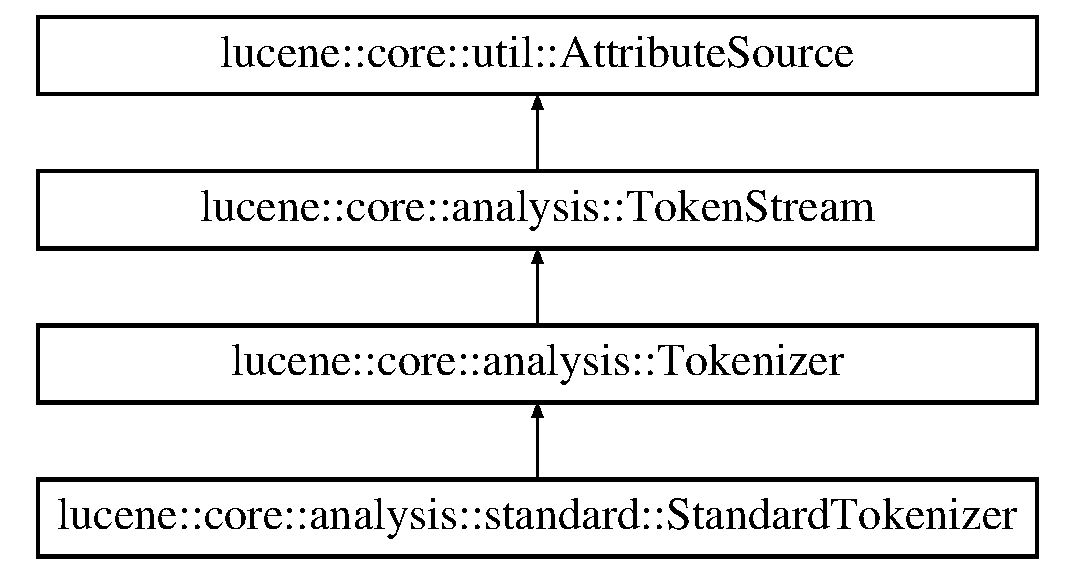
\includegraphics[height=4.000000cm]{classlucene_1_1core_1_1analysis_1_1standard_1_1StandardTokenizer}
\end{center}
\end{figure}
\subsection*{Public Member Functions}
\begin{DoxyCompactItemize}
\item 
\mbox{\hyperlink{classlucene_1_1core_1_1analysis_1_1standard_1_1StandardTokenizer_a1277d4a3ee7fd0191250c6871c2a4b87}{Standard\+Tokenizer}} ()
\item 
\mbox{\hyperlink{classlucene_1_1core_1_1analysis_1_1standard_1_1StandardTokenizer_ae0953014758400fc119c58373937abc0}{Standard\+Tokenizer}} (\mbox{\hyperlink{classlucene_1_1core_1_1util_1_1AttributeFactory}{lucene\+::core\+::util\+::\+Attribute\+Factory}} \&\mbox{\hyperlink{classlucene_1_1core_1_1util_1_1AttributeSource_a1376420a752f337a0fdb582bdf160eba}{factory}})
\item 
virtual \mbox{\hyperlink{classlucene_1_1core_1_1analysis_1_1standard_1_1StandardTokenizer_af5cadb92a403f1c41592a1be796eeb8b}{$\sim$\+Standard\+Tokenizer}} ()
\item 
void \mbox{\hyperlink{classlucene_1_1core_1_1analysis_1_1standard_1_1StandardTokenizer_ab5b2f4a086ed9ef0f196080fa7de0ceb}{Set\+Max\+Token\+Length}} (uint32\+\_\+t length)
\item 
uint32\+\_\+t \mbox{\hyperlink{classlucene_1_1core_1_1analysis_1_1standard_1_1StandardTokenizer_a8c4763c6470ab3724cd8f05191be48a2}{Get\+Max\+Token\+Length}} ()
\item 
bool \mbox{\hyperlink{classlucene_1_1core_1_1analysis_1_1standard_1_1StandardTokenizer_a5702119d01489ede9396db0794a98c41}{Increment\+Token}} () override
\item 
void \mbox{\hyperlink{classlucene_1_1core_1_1analysis_1_1standard_1_1StandardTokenizer_a733b678af865ff10e41fba9b74131872}{End}} ()
\item 
void \mbox{\hyperlink{classlucene_1_1core_1_1analysis_1_1standard_1_1StandardTokenizer_a108793659fb18bdd695e0c2be91ba730}{Close}} ()
\item 
void \mbox{\hyperlink{classlucene_1_1core_1_1analysis_1_1standard_1_1StandardTokenizer_a4d6e42ca0fcaf07cb6615643362891b3}{Reset}} ()
\end{DoxyCompactItemize}
\subsection*{Static Public Attributes}
\begin{DoxyCompactItemize}
\item 
static const uint32\+\_\+t \mbox{\hyperlink{classlucene_1_1core_1_1analysis_1_1standard_1_1StandardTokenizer_a89e87742cc1d983b876602ddf7c4d823}{A\+L\+P\+H\+A\+N\+UM}} = 0
\item 
static const uint32\+\_\+t \mbox{\hyperlink{classlucene_1_1core_1_1analysis_1_1standard_1_1StandardTokenizer_a0cc5d40f8afa24869c28e26a21ac9a9a}{N\+UM}} = 1
\item 
static const uint32\+\_\+t \mbox{\hyperlink{classlucene_1_1core_1_1analysis_1_1standard_1_1StandardTokenizer_a325a7c52ff70ac6004472ce67d2c195d}{S\+O\+U\+T\+H\+E\+A\+S\+T\+\_\+\+A\+S\+I\+AN}} = 2
\item 
static const uint32\+\_\+t \mbox{\hyperlink{classlucene_1_1core_1_1analysis_1_1standard_1_1StandardTokenizer_a7819d2406e5c2e852740b5123736e66e}{I\+D\+E\+O\+G\+R\+A\+P\+H\+IC}} = 3
\item 
static const uint32\+\_\+t \mbox{\hyperlink{classlucene_1_1core_1_1analysis_1_1standard_1_1StandardTokenizer_a9493d33d2e50179798c89ee7e21de4c8}{H\+I\+R\+A\+G\+A\+NA}} = 4
\item 
static const uint32\+\_\+t \mbox{\hyperlink{classlucene_1_1core_1_1analysis_1_1standard_1_1StandardTokenizer_a3177ce400602ef55696803cdf9cf6bd1}{K\+A\+T\+A\+K\+A\+NA}} = 5
\item 
static const uint32\+\_\+t \mbox{\hyperlink{classlucene_1_1core_1_1analysis_1_1standard_1_1StandardTokenizer_aaafb4ee36c04de9e70b96bfa4b3ffd71}{H\+A\+N\+G\+UL}} = 6
\item 
static const char $\ast$ \mbox{\hyperlink{classlucene_1_1core_1_1analysis_1_1standard_1_1StandardTokenizer_a565064bb569766d9345ab41fdd699cb0}{T\+O\+K\+E\+N\+\_\+\+T\+Y\+P\+ES}} \mbox{[}$\,$\mbox{]}
\item 
static const uint32\+\_\+t \mbox{\hyperlink{classlucene_1_1core_1_1analysis_1_1standard_1_1StandardTokenizer_ad5781b94208ea9b696dc91efac36e80d}{M\+A\+X\+\_\+\+T\+O\+K\+E\+N\+\_\+\+L\+E\+N\+G\+T\+H\+\_\+\+L\+I\+M\+IT}} = 1024 $\ast$ 1024
\end{DoxyCompactItemize}
\subsection*{Private Attributes}
\begin{DoxyCompactItemize}
\item 
int32\+\_\+t \mbox{\hyperlink{classlucene_1_1core_1_1analysis_1_1standard_1_1StandardTokenizer_a822d3e10bec987a36a17344f56e043e3}{skipped\+\_\+positions}}
\item 
int32\+\_\+t \mbox{\hyperlink{classlucene_1_1core_1_1analysis_1_1standard_1_1StandardTokenizer_a94d9646f952d3b00e2329adb31dd8ff2}{max\+\_\+token\+\_\+length}}
\item 
std\+::shared\+\_\+ptr$<$ \mbox{\hyperlink{classlucene_1_1core_1_1analysis_1_1tokenattributes_1_1CharTermAttribute}{tokenattributes\+::\+Char\+Term\+Attribute}} $>$ \mbox{\hyperlink{classlucene_1_1core_1_1analysis_1_1standard_1_1StandardTokenizer_a92fedf9b1a1985ff3f1215004684bf4d}{term\+\_\+att}}
\item 
std\+::shared\+\_\+ptr$<$ \mbox{\hyperlink{classlucene_1_1core_1_1analysis_1_1tokenattributes_1_1OffsetAttribute}{tokenattributes\+::\+Offset\+Attribute}} $>$ \mbox{\hyperlink{classlucene_1_1core_1_1analysis_1_1standard_1_1StandardTokenizer_a80ec2aca819b34dc48ad99408a39fc2d}{offset\+\_\+att}}
\item 
std\+::shared\+\_\+ptr$<$ \mbox{\hyperlink{classlucene_1_1core_1_1analysis_1_1tokenattributes_1_1PositionIncrementAttribute}{tokenattributes\+::\+Position\+Increment\+Attribute}} $>$ \mbox{\hyperlink{classlucene_1_1core_1_1analysis_1_1standard_1_1StandardTokenizer_a7fda0cbb61043d793db131ccc70eaaec}{pos\+\_\+incr\+\_\+att}}
\item 
std\+::shared\+\_\+ptr$<$ \mbox{\hyperlink{classlucene_1_1core_1_1analysis_1_1tokenattributes_1_1TypeAttribute}{tokenattributes\+::\+Type\+Attribute}} $>$ \mbox{\hyperlink{classlucene_1_1core_1_1analysis_1_1standard_1_1StandardTokenizer_ab3d625b382877b9e75fd3f05bd834e50}{type\+\_\+att}}
\item 
\mbox{\hyperlink{classlucene_1_1core_1_1analysis_1_1standard_1_1StandardTokenizerImpl}{Standard\+Tokenizer\+Impl}} \mbox{\hyperlink{classlucene_1_1core_1_1analysis_1_1standard_1_1StandardTokenizer_adb4702e24ca7dc4a5ff3e92e5249acbe}{scanner}}
\end{DoxyCompactItemize}
\subsection*{Additional Inherited Members}


\subsection{Constructor \& Destructor Documentation}
\mbox{\Hypertarget{classlucene_1_1core_1_1analysis_1_1standard_1_1StandardTokenizer_a1277d4a3ee7fd0191250c6871c2a4b87}\label{classlucene_1_1core_1_1analysis_1_1standard_1_1StandardTokenizer_a1277d4a3ee7fd0191250c6871c2a4b87}} 
\index{lucene\+::core\+::analysis\+::standard\+::\+Standard\+Tokenizer@{lucene\+::core\+::analysis\+::standard\+::\+Standard\+Tokenizer}!Standard\+Tokenizer@{Standard\+Tokenizer}}
\index{Standard\+Tokenizer@{Standard\+Tokenizer}!lucene\+::core\+::analysis\+::standard\+::\+Standard\+Tokenizer@{lucene\+::core\+::analysis\+::standard\+::\+Standard\+Tokenizer}}
\subsubsection{\texorpdfstring{Standard\+Tokenizer()}{StandardTokenizer()}\hspace{0.1cm}{\footnotesize\ttfamily [1/2]}}
{\footnotesize\ttfamily Standard\+Tokenizer\+::\+Standard\+Tokenizer (\begin{DoxyParamCaption}{ }\end{DoxyParamCaption})}

\mbox{\Hypertarget{classlucene_1_1core_1_1analysis_1_1standard_1_1StandardTokenizer_ae0953014758400fc119c58373937abc0}\label{classlucene_1_1core_1_1analysis_1_1standard_1_1StandardTokenizer_ae0953014758400fc119c58373937abc0}} 
\index{lucene\+::core\+::analysis\+::standard\+::\+Standard\+Tokenizer@{lucene\+::core\+::analysis\+::standard\+::\+Standard\+Tokenizer}!Standard\+Tokenizer@{Standard\+Tokenizer}}
\index{Standard\+Tokenizer@{Standard\+Tokenizer}!lucene\+::core\+::analysis\+::standard\+::\+Standard\+Tokenizer@{lucene\+::core\+::analysis\+::standard\+::\+Standard\+Tokenizer}}
\subsubsection{\texorpdfstring{Standard\+Tokenizer()}{StandardTokenizer()}\hspace{0.1cm}{\footnotesize\ttfamily [2/2]}}
{\footnotesize\ttfamily Standard\+Tokenizer\+::\+Standard\+Tokenizer (\begin{DoxyParamCaption}\item[{\mbox{\hyperlink{classlucene_1_1core_1_1util_1_1AttributeFactory}{lucene\+::core\+::util\+::\+Attribute\+Factory}} \&}]{factory }\end{DoxyParamCaption})\hspace{0.3cm}{\ttfamily [explicit]}}

\mbox{\Hypertarget{classlucene_1_1core_1_1analysis_1_1standard_1_1StandardTokenizer_af5cadb92a403f1c41592a1be796eeb8b}\label{classlucene_1_1core_1_1analysis_1_1standard_1_1StandardTokenizer_af5cadb92a403f1c41592a1be796eeb8b}} 
\index{lucene\+::core\+::analysis\+::standard\+::\+Standard\+Tokenizer@{lucene\+::core\+::analysis\+::standard\+::\+Standard\+Tokenizer}!````~Standard\+Tokenizer@{$\sim$\+Standard\+Tokenizer}}
\index{````~Standard\+Tokenizer@{$\sim$\+Standard\+Tokenizer}!lucene\+::core\+::analysis\+::standard\+::\+Standard\+Tokenizer@{lucene\+::core\+::analysis\+::standard\+::\+Standard\+Tokenizer}}
\subsubsection{\texorpdfstring{$\sim$\+Standard\+Tokenizer()}{~StandardTokenizer()}}
{\footnotesize\ttfamily Standard\+Tokenizer\+::$\sim$\+Standard\+Tokenizer (\begin{DoxyParamCaption}{ }\end{DoxyParamCaption})\hspace{0.3cm}{\ttfamily [virtual]}}



\subsection{Member Function Documentation}
\mbox{\Hypertarget{classlucene_1_1core_1_1analysis_1_1standard_1_1StandardTokenizer_a108793659fb18bdd695e0c2be91ba730}\label{classlucene_1_1core_1_1analysis_1_1standard_1_1StandardTokenizer_a108793659fb18bdd695e0c2be91ba730}} 
\index{lucene\+::core\+::analysis\+::standard\+::\+Standard\+Tokenizer@{lucene\+::core\+::analysis\+::standard\+::\+Standard\+Tokenizer}!Close@{Close}}
\index{Close@{Close}!lucene\+::core\+::analysis\+::standard\+::\+Standard\+Tokenizer@{lucene\+::core\+::analysis\+::standard\+::\+Standard\+Tokenizer}}
\subsubsection{\texorpdfstring{Close()}{Close()}}
{\footnotesize\ttfamily void Standard\+Tokenizer\+::\+Close (\begin{DoxyParamCaption}{ }\end{DoxyParamCaption})\hspace{0.3cm}{\ttfamily [virtual]}}



Reimplemented from \mbox{\hyperlink{classlucene_1_1core_1_1analysis_1_1TokenStream_ad7963391ddbb2c75610e3738ba5155c8}{lucene\+::core\+::analysis\+::\+Token\+Stream}}.

\mbox{\Hypertarget{classlucene_1_1core_1_1analysis_1_1standard_1_1StandardTokenizer_a733b678af865ff10e41fba9b74131872}\label{classlucene_1_1core_1_1analysis_1_1standard_1_1StandardTokenizer_a733b678af865ff10e41fba9b74131872}} 
\index{lucene\+::core\+::analysis\+::standard\+::\+Standard\+Tokenizer@{lucene\+::core\+::analysis\+::standard\+::\+Standard\+Tokenizer}!End@{End}}
\index{End@{End}!lucene\+::core\+::analysis\+::standard\+::\+Standard\+Tokenizer@{lucene\+::core\+::analysis\+::standard\+::\+Standard\+Tokenizer}}
\subsubsection{\texorpdfstring{End()}{End()}}
{\footnotesize\ttfamily void Standard\+Tokenizer\+::\+End (\begin{DoxyParamCaption}{ }\end{DoxyParamCaption})\hspace{0.3cm}{\ttfamily [virtual]}}



Reimplemented from \mbox{\hyperlink{classlucene_1_1core_1_1analysis_1_1TokenStream_a4693985ca7fb242412049a074027b8b5}{lucene\+::core\+::analysis\+::\+Token\+Stream}}.

\mbox{\Hypertarget{classlucene_1_1core_1_1analysis_1_1standard_1_1StandardTokenizer_a8c4763c6470ab3724cd8f05191be48a2}\label{classlucene_1_1core_1_1analysis_1_1standard_1_1StandardTokenizer_a8c4763c6470ab3724cd8f05191be48a2}} 
\index{lucene\+::core\+::analysis\+::standard\+::\+Standard\+Tokenizer@{lucene\+::core\+::analysis\+::standard\+::\+Standard\+Tokenizer}!Get\+Max\+Token\+Length@{Get\+Max\+Token\+Length}}
\index{Get\+Max\+Token\+Length@{Get\+Max\+Token\+Length}!lucene\+::core\+::analysis\+::standard\+::\+Standard\+Tokenizer@{lucene\+::core\+::analysis\+::standard\+::\+Standard\+Tokenizer}}
\subsubsection{\texorpdfstring{Get\+Max\+Token\+Length()}{GetMaxTokenLength()}}
{\footnotesize\ttfamily uint32\+\_\+t Standard\+Tokenizer\+::\+Get\+Max\+Token\+Length (\begin{DoxyParamCaption}{ }\end{DoxyParamCaption})}

\mbox{\Hypertarget{classlucene_1_1core_1_1analysis_1_1standard_1_1StandardTokenizer_a5702119d01489ede9396db0794a98c41}\label{classlucene_1_1core_1_1analysis_1_1standard_1_1StandardTokenizer_a5702119d01489ede9396db0794a98c41}} 
\index{lucene\+::core\+::analysis\+::standard\+::\+Standard\+Tokenizer@{lucene\+::core\+::analysis\+::standard\+::\+Standard\+Tokenizer}!Increment\+Token@{Increment\+Token}}
\index{Increment\+Token@{Increment\+Token}!lucene\+::core\+::analysis\+::standard\+::\+Standard\+Tokenizer@{lucene\+::core\+::analysis\+::standard\+::\+Standard\+Tokenizer}}
\subsubsection{\texorpdfstring{Increment\+Token()}{IncrementToken()}}
{\footnotesize\ttfamily bool Standard\+Tokenizer\+::\+Increment\+Token (\begin{DoxyParamCaption}{ }\end{DoxyParamCaption})\hspace{0.3cm}{\ttfamily [override]}, {\ttfamily [virtual]}}



Implements \mbox{\hyperlink{classlucene_1_1core_1_1analysis_1_1TokenStream_a614d4ea24a354d6f4354b4941b5124e2}{lucene\+::core\+::analysis\+::\+Token\+Stream}}.

\mbox{\Hypertarget{classlucene_1_1core_1_1analysis_1_1standard_1_1StandardTokenizer_a4d6e42ca0fcaf07cb6615643362891b3}\label{classlucene_1_1core_1_1analysis_1_1standard_1_1StandardTokenizer_a4d6e42ca0fcaf07cb6615643362891b3}} 
\index{lucene\+::core\+::analysis\+::standard\+::\+Standard\+Tokenizer@{lucene\+::core\+::analysis\+::standard\+::\+Standard\+Tokenizer}!Reset@{Reset}}
\index{Reset@{Reset}!lucene\+::core\+::analysis\+::standard\+::\+Standard\+Tokenizer@{lucene\+::core\+::analysis\+::standard\+::\+Standard\+Tokenizer}}
\subsubsection{\texorpdfstring{Reset()}{Reset()}}
{\footnotesize\ttfamily void Standard\+Tokenizer\+::\+Reset (\begin{DoxyParamCaption}{ }\end{DoxyParamCaption})\hspace{0.3cm}{\ttfamily [virtual]}}



Implements \mbox{\hyperlink{classlucene_1_1core_1_1analysis_1_1TokenStream_ae24622f4bc0aeaf0bef924ff1661e023}{lucene\+::core\+::analysis\+::\+Token\+Stream}}.

\mbox{\Hypertarget{classlucene_1_1core_1_1analysis_1_1standard_1_1StandardTokenizer_ab5b2f4a086ed9ef0f196080fa7de0ceb}\label{classlucene_1_1core_1_1analysis_1_1standard_1_1StandardTokenizer_ab5b2f4a086ed9ef0f196080fa7de0ceb}} 
\index{lucene\+::core\+::analysis\+::standard\+::\+Standard\+Tokenizer@{lucene\+::core\+::analysis\+::standard\+::\+Standard\+Tokenizer}!Set\+Max\+Token\+Length@{Set\+Max\+Token\+Length}}
\index{Set\+Max\+Token\+Length@{Set\+Max\+Token\+Length}!lucene\+::core\+::analysis\+::standard\+::\+Standard\+Tokenizer@{lucene\+::core\+::analysis\+::standard\+::\+Standard\+Tokenizer}}
\subsubsection{\texorpdfstring{Set\+Max\+Token\+Length()}{SetMaxTokenLength()}}
{\footnotesize\ttfamily void Standard\+Tokenizer\+::\+Set\+Max\+Token\+Length (\begin{DoxyParamCaption}\item[{uint32\+\_\+t}]{length }\end{DoxyParamCaption})}



\subsection{Member Data Documentation}
\mbox{\Hypertarget{classlucene_1_1core_1_1analysis_1_1standard_1_1StandardTokenizer_a89e87742cc1d983b876602ddf7c4d823}\label{classlucene_1_1core_1_1analysis_1_1standard_1_1StandardTokenizer_a89e87742cc1d983b876602ddf7c4d823}} 
\index{lucene\+::core\+::analysis\+::standard\+::\+Standard\+Tokenizer@{lucene\+::core\+::analysis\+::standard\+::\+Standard\+Tokenizer}!A\+L\+P\+H\+A\+N\+UM@{A\+L\+P\+H\+A\+N\+UM}}
\index{A\+L\+P\+H\+A\+N\+UM@{A\+L\+P\+H\+A\+N\+UM}!lucene\+::core\+::analysis\+::standard\+::\+Standard\+Tokenizer@{lucene\+::core\+::analysis\+::standard\+::\+Standard\+Tokenizer}}
\subsubsection{\texorpdfstring{A\+L\+P\+H\+A\+N\+UM}{ALPHANUM}}
{\footnotesize\ttfamily const uint32\+\_\+t Standard\+Tokenizer\+::\+A\+L\+P\+H\+A\+N\+UM = 0\hspace{0.3cm}{\ttfamily [static]}}

\mbox{\Hypertarget{classlucene_1_1core_1_1analysis_1_1standard_1_1StandardTokenizer_aaafb4ee36c04de9e70b96bfa4b3ffd71}\label{classlucene_1_1core_1_1analysis_1_1standard_1_1StandardTokenizer_aaafb4ee36c04de9e70b96bfa4b3ffd71}} 
\index{lucene\+::core\+::analysis\+::standard\+::\+Standard\+Tokenizer@{lucene\+::core\+::analysis\+::standard\+::\+Standard\+Tokenizer}!H\+A\+N\+G\+UL@{H\+A\+N\+G\+UL}}
\index{H\+A\+N\+G\+UL@{H\+A\+N\+G\+UL}!lucene\+::core\+::analysis\+::standard\+::\+Standard\+Tokenizer@{lucene\+::core\+::analysis\+::standard\+::\+Standard\+Tokenizer}}
\subsubsection{\texorpdfstring{H\+A\+N\+G\+UL}{HANGUL}}
{\footnotesize\ttfamily const uint32\+\_\+t Standard\+Tokenizer\+::\+H\+A\+N\+G\+UL = 6\hspace{0.3cm}{\ttfamily [static]}}

\mbox{\Hypertarget{classlucene_1_1core_1_1analysis_1_1standard_1_1StandardTokenizer_a9493d33d2e50179798c89ee7e21de4c8}\label{classlucene_1_1core_1_1analysis_1_1standard_1_1StandardTokenizer_a9493d33d2e50179798c89ee7e21de4c8}} 
\index{lucene\+::core\+::analysis\+::standard\+::\+Standard\+Tokenizer@{lucene\+::core\+::analysis\+::standard\+::\+Standard\+Tokenizer}!H\+I\+R\+A\+G\+A\+NA@{H\+I\+R\+A\+G\+A\+NA}}
\index{H\+I\+R\+A\+G\+A\+NA@{H\+I\+R\+A\+G\+A\+NA}!lucene\+::core\+::analysis\+::standard\+::\+Standard\+Tokenizer@{lucene\+::core\+::analysis\+::standard\+::\+Standard\+Tokenizer}}
\subsubsection{\texorpdfstring{H\+I\+R\+A\+G\+A\+NA}{HIRAGANA}}
{\footnotesize\ttfamily const uint32\+\_\+t Standard\+Tokenizer\+::\+H\+I\+R\+A\+G\+A\+NA = 4\hspace{0.3cm}{\ttfamily [static]}}

\mbox{\Hypertarget{classlucene_1_1core_1_1analysis_1_1standard_1_1StandardTokenizer_a7819d2406e5c2e852740b5123736e66e}\label{classlucene_1_1core_1_1analysis_1_1standard_1_1StandardTokenizer_a7819d2406e5c2e852740b5123736e66e}} 
\index{lucene\+::core\+::analysis\+::standard\+::\+Standard\+Tokenizer@{lucene\+::core\+::analysis\+::standard\+::\+Standard\+Tokenizer}!I\+D\+E\+O\+G\+R\+A\+P\+H\+IC@{I\+D\+E\+O\+G\+R\+A\+P\+H\+IC}}
\index{I\+D\+E\+O\+G\+R\+A\+P\+H\+IC@{I\+D\+E\+O\+G\+R\+A\+P\+H\+IC}!lucene\+::core\+::analysis\+::standard\+::\+Standard\+Tokenizer@{lucene\+::core\+::analysis\+::standard\+::\+Standard\+Tokenizer}}
\subsubsection{\texorpdfstring{I\+D\+E\+O\+G\+R\+A\+P\+H\+IC}{IDEOGRAPHIC}}
{\footnotesize\ttfamily const uint32\+\_\+t Standard\+Tokenizer\+::\+I\+D\+E\+O\+G\+R\+A\+P\+H\+IC = 3\hspace{0.3cm}{\ttfamily [static]}}

\mbox{\Hypertarget{classlucene_1_1core_1_1analysis_1_1standard_1_1StandardTokenizer_a3177ce400602ef55696803cdf9cf6bd1}\label{classlucene_1_1core_1_1analysis_1_1standard_1_1StandardTokenizer_a3177ce400602ef55696803cdf9cf6bd1}} 
\index{lucene\+::core\+::analysis\+::standard\+::\+Standard\+Tokenizer@{lucene\+::core\+::analysis\+::standard\+::\+Standard\+Tokenizer}!K\+A\+T\+A\+K\+A\+NA@{K\+A\+T\+A\+K\+A\+NA}}
\index{K\+A\+T\+A\+K\+A\+NA@{K\+A\+T\+A\+K\+A\+NA}!lucene\+::core\+::analysis\+::standard\+::\+Standard\+Tokenizer@{lucene\+::core\+::analysis\+::standard\+::\+Standard\+Tokenizer}}
\subsubsection{\texorpdfstring{K\+A\+T\+A\+K\+A\+NA}{KATAKANA}}
{\footnotesize\ttfamily const uint32\+\_\+t Standard\+Tokenizer\+::\+K\+A\+T\+A\+K\+A\+NA = 5\hspace{0.3cm}{\ttfamily [static]}}

\mbox{\Hypertarget{classlucene_1_1core_1_1analysis_1_1standard_1_1StandardTokenizer_a94d9646f952d3b00e2329adb31dd8ff2}\label{classlucene_1_1core_1_1analysis_1_1standard_1_1StandardTokenizer_a94d9646f952d3b00e2329adb31dd8ff2}} 
\index{lucene\+::core\+::analysis\+::standard\+::\+Standard\+Tokenizer@{lucene\+::core\+::analysis\+::standard\+::\+Standard\+Tokenizer}!max\+\_\+token\+\_\+length@{max\+\_\+token\+\_\+length}}
\index{max\+\_\+token\+\_\+length@{max\+\_\+token\+\_\+length}!lucene\+::core\+::analysis\+::standard\+::\+Standard\+Tokenizer@{lucene\+::core\+::analysis\+::standard\+::\+Standard\+Tokenizer}}
\subsubsection{\texorpdfstring{max\+\_\+token\+\_\+length}{max\_token\_length}}
{\footnotesize\ttfamily int32\+\_\+t lucene\+::core\+::analysis\+::standard\+::\+Standard\+Tokenizer\+::max\+\_\+token\+\_\+length\hspace{0.3cm}{\ttfamily [private]}}

\mbox{\Hypertarget{classlucene_1_1core_1_1analysis_1_1standard_1_1StandardTokenizer_ad5781b94208ea9b696dc91efac36e80d}\label{classlucene_1_1core_1_1analysis_1_1standard_1_1StandardTokenizer_ad5781b94208ea9b696dc91efac36e80d}} 
\index{lucene\+::core\+::analysis\+::standard\+::\+Standard\+Tokenizer@{lucene\+::core\+::analysis\+::standard\+::\+Standard\+Tokenizer}!M\+A\+X\+\_\+\+T\+O\+K\+E\+N\+\_\+\+L\+E\+N\+G\+T\+H\+\_\+\+L\+I\+M\+IT@{M\+A\+X\+\_\+\+T\+O\+K\+E\+N\+\_\+\+L\+E\+N\+G\+T\+H\+\_\+\+L\+I\+M\+IT}}
\index{M\+A\+X\+\_\+\+T\+O\+K\+E\+N\+\_\+\+L\+E\+N\+G\+T\+H\+\_\+\+L\+I\+M\+IT@{M\+A\+X\+\_\+\+T\+O\+K\+E\+N\+\_\+\+L\+E\+N\+G\+T\+H\+\_\+\+L\+I\+M\+IT}!lucene\+::core\+::analysis\+::standard\+::\+Standard\+Tokenizer@{lucene\+::core\+::analysis\+::standard\+::\+Standard\+Tokenizer}}
\subsubsection{\texorpdfstring{M\+A\+X\+\_\+\+T\+O\+K\+E\+N\+\_\+\+L\+E\+N\+G\+T\+H\+\_\+\+L\+I\+M\+IT}{MAX\_TOKEN\_LENGTH\_LIMIT}}
{\footnotesize\ttfamily const uint32\+\_\+t Standard\+Tokenizer\+::\+M\+A\+X\+\_\+\+T\+O\+K\+E\+N\+\_\+\+L\+E\+N\+G\+T\+H\+\_\+\+L\+I\+M\+IT = 1024 $\ast$ 1024\hspace{0.3cm}{\ttfamily [static]}}

\mbox{\Hypertarget{classlucene_1_1core_1_1analysis_1_1standard_1_1StandardTokenizer_a0cc5d40f8afa24869c28e26a21ac9a9a}\label{classlucene_1_1core_1_1analysis_1_1standard_1_1StandardTokenizer_a0cc5d40f8afa24869c28e26a21ac9a9a}} 
\index{lucene\+::core\+::analysis\+::standard\+::\+Standard\+Tokenizer@{lucene\+::core\+::analysis\+::standard\+::\+Standard\+Tokenizer}!N\+UM@{N\+UM}}
\index{N\+UM@{N\+UM}!lucene\+::core\+::analysis\+::standard\+::\+Standard\+Tokenizer@{lucene\+::core\+::analysis\+::standard\+::\+Standard\+Tokenizer}}
\subsubsection{\texorpdfstring{N\+UM}{NUM}}
{\footnotesize\ttfamily const uint32\+\_\+t Standard\+Tokenizer\+::\+N\+UM = 1\hspace{0.3cm}{\ttfamily [static]}}

\mbox{\Hypertarget{classlucene_1_1core_1_1analysis_1_1standard_1_1StandardTokenizer_a80ec2aca819b34dc48ad99408a39fc2d}\label{classlucene_1_1core_1_1analysis_1_1standard_1_1StandardTokenizer_a80ec2aca819b34dc48ad99408a39fc2d}} 
\index{lucene\+::core\+::analysis\+::standard\+::\+Standard\+Tokenizer@{lucene\+::core\+::analysis\+::standard\+::\+Standard\+Tokenizer}!offset\+\_\+att@{offset\+\_\+att}}
\index{offset\+\_\+att@{offset\+\_\+att}!lucene\+::core\+::analysis\+::standard\+::\+Standard\+Tokenizer@{lucene\+::core\+::analysis\+::standard\+::\+Standard\+Tokenizer}}
\subsubsection{\texorpdfstring{offset\+\_\+att}{offset\_att}}
{\footnotesize\ttfamily std\+::shared\+\_\+ptr$<$\mbox{\hyperlink{classlucene_1_1core_1_1analysis_1_1tokenattributes_1_1OffsetAttribute}{tokenattributes\+::\+Offset\+Attribute}}$>$ lucene\+::core\+::analysis\+::standard\+::\+Standard\+Tokenizer\+::offset\+\_\+att\hspace{0.3cm}{\ttfamily [private]}}

\mbox{\Hypertarget{classlucene_1_1core_1_1analysis_1_1standard_1_1StandardTokenizer_a7fda0cbb61043d793db131ccc70eaaec}\label{classlucene_1_1core_1_1analysis_1_1standard_1_1StandardTokenizer_a7fda0cbb61043d793db131ccc70eaaec}} 
\index{lucene\+::core\+::analysis\+::standard\+::\+Standard\+Tokenizer@{lucene\+::core\+::analysis\+::standard\+::\+Standard\+Tokenizer}!pos\+\_\+incr\+\_\+att@{pos\+\_\+incr\+\_\+att}}
\index{pos\+\_\+incr\+\_\+att@{pos\+\_\+incr\+\_\+att}!lucene\+::core\+::analysis\+::standard\+::\+Standard\+Tokenizer@{lucene\+::core\+::analysis\+::standard\+::\+Standard\+Tokenizer}}
\subsubsection{\texorpdfstring{pos\+\_\+incr\+\_\+att}{pos\_incr\_att}}
{\footnotesize\ttfamily std\+::shared\+\_\+ptr$<$\mbox{\hyperlink{classlucene_1_1core_1_1analysis_1_1tokenattributes_1_1PositionIncrementAttribute}{tokenattributes\+::\+Position\+Increment\+Attribute}}$>$ lucene\+::core\+::analysis\+::standard\+::\+Standard\+Tokenizer\+::pos\+\_\+incr\+\_\+att\hspace{0.3cm}{\ttfamily [private]}}

\mbox{\Hypertarget{classlucene_1_1core_1_1analysis_1_1standard_1_1StandardTokenizer_adb4702e24ca7dc4a5ff3e92e5249acbe}\label{classlucene_1_1core_1_1analysis_1_1standard_1_1StandardTokenizer_adb4702e24ca7dc4a5ff3e92e5249acbe}} 
\index{lucene\+::core\+::analysis\+::standard\+::\+Standard\+Tokenizer@{lucene\+::core\+::analysis\+::standard\+::\+Standard\+Tokenizer}!scanner@{scanner}}
\index{scanner@{scanner}!lucene\+::core\+::analysis\+::standard\+::\+Standard\+Tokenizer@{lucene\+::core\+::analysis\+::standard\+::\+Standard\+Tokenizer}}
\subsubsection{\texorpdfstring{scanner}{scanner}}
{\footnotesize\ttfamily \mbox{\hyperlink{classlucene_1_1core_1_1analysis_1_1standard_1_1StandardTokenizerImpl}{Standard\+Tokenizer\+Impl}} lucene\+::core\+::analysis\+::standard\+::\+Standard\+Tokenizer\+::scanner\hspace{0.3cm}{\ttfamily [private]}}

\mbox{\Hypertarget{classlucene_1_1core_1_1analysis_1_1standard_1_1StandardTokenizer_a822d3e10bec987a36a17344f56e043e3}\label{classlucene_1_1core_1_1analysis_1_1standard_1_1StandardTokenizer_a822d3e10bec987a36a17344f56e043e3}} 
\index{lucene\+::core\+::analysis\+::standard\+::\+Standard\+Tokenizer@{lucene\+::core\+::analysis\+::standard\+::\+Standard\+Tokenizer}!skipped\+\_\+positions@{skipped\+\_\+positions}}
\index{skipped\+\_\+positions@{skipped\+\_\+positions}!lucene\+::core\+::analysis\+::standard\+::\+Standard\+Tokenizer@{lucene\+::core\+::analysis\+::standard\+::\+Standard\+Tokenizer}}
\subsubsection{\texorpdfstring{skipped\+\_\+positions}{skipped\_positions}}
{\footnotesize\ttfamily int32\+\_\+t lucene\+::core\+::analysis\+::standard\+::\+Standard\+Tokenizer\+::skipped\+\_\+positions\hspace{0.3cm}{\ttfamily [private]}}

\mbox{\Hypertarget{classlucene_1_1core_1_1analysis_1_1standard_1_1StandardTokenizer_a325a7c52ff70ac6004472ce67d2c195d}\label{classlucene_1_1core_1_1analysis_1_1standard_1_1StandardTokenizer_a325a7c52ff70ac6004472ce67d2c195d}} 
\index{lucene\+::core\+::analysis\+::standard\+::\+Standard\+Tokenizer@{lucene\+::core\+::analysis\+::standard\+::\+Standard\+Tokenizer}!S\+O\+U\+T\+H\+E\+A\+S\+T\+\_\+\+A\+S\+I\+AN@{S\+O\+U\+T\+H\+E\+A\+S\+T\+\_\+\+A\+S\+I\+AN}}
\index{S\+O\+U\+T\+H\+E\+A\+S\+T\+\_\+\+A\+S\+I\+AN@{S\+O\+U\+T\+H\+E\+A\+S\+T\+\_\+\+A\+S\+I\+AN}!lucene\+::core\+::analysis\+::standard\+::\+Standard\+Tokenizer@{lucene\+::core\+::analysis\+::standard\+::\+Standard\+Tokenizer}}
\subsubsection{\texorpdfstring{S\+O\+U\+T\+H\+E\+A\+S\+T\+\_\+\+A\+S\+I\+AN}{SOUTHEAST\_ASIAN}}
{\footnotesize\ttfamily const uint32\+\_\+t Standard\+Tokenizer\+::\+S\+O\+U\+T\+H\+E\+A\+S\+T\+\_\+\+A\+S\+I\+AN = 2\hspace{0.3cm}{\ttfamily [static]}}

\mbox{\Hypertarget{classlucene_1_1core_1_1analysis_1_1standard_1_1StandardTokenizer_a92fedf9b1a1985ff3f1215004684bf4d}\label{classlucene_1_1core_1_1analysis_1_1standard_1_1StandardTokenizer_a92fedf9b1a1985ff3f1215004684bf4d}} 
\index{lucene\+::core\+::analysis\+::standard\+::\+Standard\+Tokenizer@{lucene\+::core\+::analysis\+::standard\+::\+Standard\+Tokenizer}!term\+\_\+att@{term\+\_\+att}}
\index{term\+\_\+att@{term\+\_\+att}!lucene\+::core\+::analysis\+::standard\+::\+Standard\+Tokenizer@{lucene\+::core\+::analysis\+::standard\+::\+Standard\+Tokenizer}}
\subsubsection{\texorpdfstring{term\+\_\+att}{term\_att}}
{\footnotesize\ttfamily std\+::shared\+\_\+ptr$<$\mbox{\hyperlink{classlucene_1_1core_1_1analysis_1_1tokenattributes_1_1CharTermAttribute}{tokenattributes\+::\+Char\+Term\+Attribute}}$>$ lucene\+::core\+::analysis\+::standard\+::\+Standard\+Tokenizer\+::term\+\_\+att\hspace{0.3cm}{\ttfamily [private]}}

\mbox{\Hypertarget{classlucene_1_1core_1_1analysis_1_1standard_1_1StandardTokenizer_a565064bb569766d9345ab41fdd699cb0}\label{classlucene_1_1core_1_1analysis_1_1standard_1_1StandardTokenizer_a565064bb569766d9345ab41fdd699cb0}} 
\index{lucene\+::core\+::analysis\+::standard\+::\+Standard\+Tokenizer@{lucene\+::core\+::analysis\+::standard\+::\+Standard\+Tokenizer}!T\+O\+K\+E\+N\+\_\+\+T\+Y\+P\+ES@{T\+O\+K\+E\+N\+\_\+\+T\+Y\+P\+ES}}
\index{T\+O\+K\+E\+N\+\_\+\+T\+Y\+P\+ES@{T\+O\+K\+E\+N\+\_\+\+T\+Y\+P\+ES}!lucene\+::core\+::analysis\+::standard\+::\+Standard\+Tokenizer@{lucene\+::core\+::analysis\+::standard\+::\+Standard\+Tokenizer}}
\subsubsection{\texorpdfstring{T\+O\+K\+E\+N\+\_\+\+T\+Y\+P\+ES}{TOKEN\_TYPES}}
{\footnotesize\ttfamily const char $\ast$ Standard\+Tokenizer\+::\+T\+O\+K\+E\+N\+\_\+\+T\+Y\+P\+ES\hspace{0.3cm}{\ttfamily [static]}}

{\bfseries Initial value\+:}
\begin{DoxyCode}
\DoxyCodeLine{= \{}
\DoxyCodeLine{  \textcolor{stringliteral}{"<ALPHANUM>"},}
\DoxyCodeLine{  \textcolor{stringliteral}{"<NUM>"},}
\DoxyCodeLine{  \textcolor{stringliteral}{"<SOUTHEAST\_ASIAN>"},}
\DoxyCodeLine{  \textcolor{stringliteral}{"<IDEOGRAPHIC>"},}
\DoxyCodeLine{  \textcolor{stringliteral}{"<HIRAGANA>"},}
\DoxyCodeLine{  \textcolor{stringliteral}{"<KATAKANA>"},}
\DoxyCodeLine{  \textcolor{stringliteral}{"<HANGUL>"}}
\DoxyCodeLine{\}}
\end{DoxyCode}
\mbox{\Hypertarget{classlucene_1_1core_1_1analysis_1_1standard_1_1StandardTokenizer_ab3d625b382877b9e75fd3f05bd834e50}\label{classlucene_1_1core_1_1analysis_1_1standard_1_1StandardTokenizer_ab3d625b382877b9e75fd3f05bd834e50}} 
\index{lucene\+::core\+::analysis\+::standard\+::\+Standard\+Tokenizer@{lucene\+::core\+::analysis\+::standard\+::\+Standard\+Tokenizer}!type\+\_\+att@{type\+\_\+att}}
\index{type\+\_\+att@{type\+\_\+att}!lucene\+::core\+::analysis\+::standard\+::\+Standard\+Tokenizer@{lucene\+::core\+::analysis\+::standard\+::\+Standard\+Tokenizer}}
\subsubsection{\texorpdfstring{type\+\_\+att}{type\_att}}
{\footnotesize\ttfamily std\+::shared\+\_\+ptr$<$\mbox{\hyperlink{classlucene_1_1core_1_1analysis_1_1tokenattributes_1_1TypeAttribute}{tokenattributes\+::\+Type\+Attribute}}$>$ lucene\+::core\+::analysis\+::standard\+::\+Standard\+Tokenizer\+::type\+\_\+att\hspace{0.3cm}{\ttfamily [private]}}



The documentation for this class was generated from the following files\+:\begin{DoxyCompactItemize}
\item 
Analysis/\mbox{\hyperlink{Standard_8h}{Standard.\+h}}\item 
Analysis/\mbox{\hyperlink{Standard_8cpp}{Standard.\+cpp}}\end{DoxyCompactItemize}

\hypertarget{classlucene_1_1core_1_1analysis_1_1standard_1_1StandardTokenizerImpl}{}\section{lucene\+:\+:core\+:\+:analysis\+:\+:standard\+:\+:Standard\+Tokenizer\+Impl Class Reference}
\label{classlucene_1_1core_1_1analysis_1_1standard_1_1StandardTokenizerImpl}\index{lucene\+::core\+::analysis\+::standard\+::\+Standard\+Tokenizer\+Impl@{lucene\+::core\+::analysis\+::standard\+::\+Standard\+Tokenizer\+Impl}}


{\ttfamily \#include $<$Standard.\+h$>$}

\subsection*{Public Member Functions}
\begin{DoxyCompactItemize}
\item 
\mbox{\hyperlink{classlucene_1_1core_1_1analysis_1_1standard_1_1StandardTokenizerImpl_a64aeb3d3c5c64b3c099a9042930d2072}{Standard\+Tokenizer\+Impl}} (\mbox{\hyperlink{classlucene_1_1core_1_1analysis_1_1Reader}{lucene\+::core\+::analysis\+::\+Reader}} $\ast$in)
\item 
\mbox{\hyperlink{classlucene_1_1core_1_1analysis_1_1standard_1_1StandardTokenizerImpl_a7b85d18cb75dd13793a2c067aa41eb0a}{$\sim$\+Standard\+Tokenizer\+Impl}} ()
\item 
void \mbox{\hyperlink{classlucene_1_1core_1_1analysis_1_1standard_1_1StandardTokenizerImpl_afc6d8904d6816baa27c54471da7f8755}{Set\+Buffer\+Size}} (uint32\+\_\+t length)
\item 
uint32\+\_\+t \mbox{\hyperlink{classlucene_1_1core_1_1analysis_1_1standard_1_1StandardTokenizerImpl_a4198bd2f50a136429db69c6f4025b571}{Get\+Next\+Token}} ()
\item 
void \mbox{\hyperlink{classlucene_1_1core_1_1analysis_1_1standard_1_1StandardTokenizerImpl_a8e389a9a4f8659fcdaead22795c132f3}{Get\+Text}} (\mbox{\hyperlink{classlucene_1_1core_1_1analysis_1_1tokenattributes_1_1CharTermAttribute}{tokenattributes\+::\+Char\+Term\+Attribute}} \&term\+\_\+att)
\item 
uint32\+\_\+t \mbox{\hyperlink{classlucene_1_1core_1_1analysis_1_1standard_1_1StandardTokenizerImpl_a8305da33749783d1e360abea1d384adb}{Yy\+Length}} ()
\item 
uint32\+\_\+t \mbox{\hyperlink{classlucene_1_1core_1_1analysis_1_1standard_1_1StandardTokenizerImpl_a1dec98b86d7ce0b2dd6a674380599f6c}{Yy\+Char}} ()
\item 
void \mbox{\hyperlink{classlucene_1_1core_1_1analysis_1_1standard_1_1StandardTokenizerImpl_accacb4bb2516823080aaaf0d09855958}{Yy\+Reset}} (\mbox{\hyperlink{classlucene_1_1core_1_1analysis_1_1Reader}{lucene\+::core\+::analysis\+::\+Reader}} $\ast$reader)
\end{DoxyCompactItemize}
\subsection*{Static Public Attributes}
\begin{DoxyCompactItemize}
\item 
static const int32\+\_\+t \mbox{\hyperlink{classlucene_1_1core_1_1analysis_1_1standard_1_1StandardTokenizerImpl_a9df3ece23b5c2072b3f9dde3405f56d2}{Y\+Y\+E\+OF}} = -\/1
\end{DoxyCompactItemize}


\subsection{Constructor \& Destructor Documentation}
\mbox{\Hypertarget{classlucene_1_1core_1_1analysis_1_1standard_1_1StandardTokenizerImpl_a64aeb3d3c5c64b3c099a9042930d2072}\label{classlucene_1_1core_1_1analysis_1_1standard_1_1StandardTokenizerImpl_a64aeb3d3c5c64b3c099a9042930d2072}} 
\index{lucene\+::core\+::analysis\+::standard\+::\+Standard\+Tokenizer\+Impl@{lucene\+::core\+::analysis\+::standard\+::\+Standard\+Tokenizer\+Impl}!Standard\+Tokenizer\+Impl@{Standard\+Tokenizer\+Impl}}
\index{Standard\+Tokenizer\+Impl@{Standard\+Tokenizer\+Impl}!lucene\+::core\+::analysis\+::standard\+::\+Standard\+Tokenizer\+Impl@{lucene\+::core\+::analysis\+::standard\+::\+Standard\+Tokenizer\+Impl}}
\subsubsection{\texorpdfstring{Standard\+Tokenizer\+Impl()}{StandardTokenizerImpl()}}
{\footnotesize\ttfamily Standard\+Tokenizer\+Impl\+::\+Standard\+Tokenizer\+Impl (\begin{DoxyParamCaption}\item[{\mbox{\hyperlink{classlucene_1_1core_1_1analysis_1_1Reader}{lucene\+::core\+::analysis\+::\+Reader}} $\ast$}]{in }\end{DoxyParamCaption})\hspace{0.3cm}{\ttfamily [explicit]}}

\mbox{\Hypertarget{classlucene_1_1core_1_1analysis_1_1standard_1_1StandardTokenizerImpl_a7b85d18cb75dd13793a2c067aa41eb0a}\label{classlucene_1_1core_1_1analysis_1_1standard_1_1StandardTokenizerImpl_a7b85d18cb75dd13793a2c067aa41eb0a}} 
\index{lucene\+::core\+::analysis\+::standard\+::\+Standard\+Tokenizer\+Impl@{lucene\+::core\+::analysis\+::standard\+::\+Standard\+Tokenizer\+Impl}!````~Standard\+Tokenizer\+Impl@{$\sim$\+Standard\+Tokenizer\+Impl}}
\index{````~Standard\+Tokenizer\+Impl@{$\sim$\+Standard\+Tokenizer\+Impl}!lucene\+::core\+::analysis\+::standard\+::\+Standard\+Tokenizer\+Impl@{lucene\+::core\+::analysis\+::standard\+::\+Standard\+Tokenizer\+Impl}}
\subsubsection{\texorpdfstring{$\sim$\+Standard\+Tokenizer\+Impl()}{~StandardTokenizerImpl()}}
{\footnotesize\ttfamily Standard\+Tokenizer\+Impl\+::$\sim$\+Standard\+Tokenizer\+Impl (\begin{DoxyParamCaption}{ }\end{DoxyParamCaption})}



\subsection{Member Function Documentation}
\mbox{\Hypertarget{classlucene_1_1core_1_1analysis_1_1standard_1_1StandardTokenizerImpl_a4198bd2f50a136429db69c6f4025b571}\label{classlucene_1_1core_1_1analysis_1_1standard_1_1StandardTokenizerImpl_a4198bd2f50a136429db69c6f4025b571}} 
\index{lucene\+::core\+::analysis\+::standard\+::\+Standard\+Tokenizer\+Impl@{lucene\+::core\+::analysis\+::standard\+::\+Standard\+Tokenizer\+Impl}!Get\+Next\+Token@{Get\+Next\+Token}}
\index{Get\+Next\+Token@{Get\+Next\+Token}!lucene\+::core\+::analysis\+::standard\+::\+Standard\+Tokenizer\+Impl@{lucene\+::core\+::analysis\+::standard\+::\+Standard\+Tokenizer\+Impl}}
\subsubsection{\texorpdfstring{Get\+Next\+Token()}{GetNextToken()}}
{\footnotesize\ttfamily uint32\+\_\+t Standard\+Tokenizer\+Impl\+::\+Get\+Next\+Token (\begin{DoxyParamCaption}{ }\end{DoxyParamCaption})}

\mbox{\Hypertarget{classlucene_1_1core_1_1analysis_1_1standard_1_1StandardTokenizerImpl_a8e389a9a4f8659fcdaead22795c132f3}\label{classlucene_1_1core_1_1analysis_1_1standard_1_1StandardTokenizerImpl_a8e389a9a4f8659fcdaead22795c132f3}} 
\index{lucene\+::core\+::analysis\+::standard\+::\+Standard\+Tokenizer\+Impl@{lucene\+::core\+::analysis\+::standard\+::\+Standard\+Tokenizer\+Impl}!Get\+Text@{Get\+Text}}
\index{Get\+Text@{Get\+Text}!lucene\+::core\+::analysis\+::standard\+::\+Standard\+Tokenizer\+Impl@{lucene\+::core\+::analysis\+::standard\+::\+Standard\+Tokenizer\+Impl}}
\subsubsection{\texorpdfstring{Get\+Text()}{GetText()}}
{\footnotesize\ttfamily void Standard\+Tokenizer\+Impl\+::\+Get\+Text (\begin{DoxyParamCaption}\item[{\mbox{\hyperlink{classlucene_1_1core_1_1analysis_1_1tokenattributes_1_1CharTermAttribute}{tokenattributes\+::\+Char\+Term\+Attribute}} \&}]{term\+\_\+att }\end{DoxyParamCaption})}

\mbox{\Hypertarget{classlucene_1_1core_1_1analysis_1_1standard_1_1StandardTokenizerImpl_afc6d8904d6816baa27c54471da7f8755}\label{classlucene_1_1core_1_1analysis_1_1standard_1_1StandardTokenizerImpl_afc6d8904d6816baa27c54471da7f8755}} 
\index{lucene\+::core\+::analysis\+::standard\+::\+Standard\+Tokenizer\+Impl@{lucene\+::core\+::analysis\+::standard\+::\+Standard\+Tokenizer\+Impl}!Set\+Buffer\+Size@{Set\+Buffer\+Size}}
\index{Set\+Buffer\+Size@{Set\+Buffer\+Size}!lucene\+::core\+::analysis\+::standard\+::\+Standard\+Tokenizer\+Impl@{lucene\+::core\+::analysis\+::standard\+::\+Standard\+Tokenizer\+Impl}}
\subsubsection{\texorpdfstring{Set\+Buffer\+Size()}{SetBufferSize()}}
{\footnotesize\ttfamily void Standard\+Tokenizer\+Impl\+::\+Set\+Buffer\+Size (\begin{DoxyParamCaption}\item[{uint32\+\_\+t}]{length }\end{DoxyParamCaption})}

\mbox{\Hypertarget{classlucene_1_1core_1_1analysis_1_1standard_1_1StandardTokenizerImpl_a1dec98b86d7ce0b2dd6a674380599f6c}\label{classlucene_1_1core_1_1analysis_1_1standard_1_1StandardTokenizerImpl_a1dec98b86d7ce0b2dd6a674380599f6c}} 
\index{lucene\+::core\+::analysis\+::standard\+::\+Standard\+Tokenizer\+Impl@{lucene\+::core\+::analysis\+::standard\+::\+Standard\+Tokenizer\+Impl}!Yy\+Char@{Yy\+Char}}
\index{Yy\+Char@{Yy\+Char}!lucene\+::core\+::analysis\+::standard\+::\+Standard\+Tokenizer\+Impl@{lucene\+::core\+::analysis\+::standard\+::\+Standard\+Tokenizer\+Impl}}
\subsubsection{\texorpdfstring{Yy\+Char()}{YyChar()}}
{\footnotesize\ttfamily uint32\+\_\+t Standard\+Tokenizer\+Impl\+::\+Yy\+Char (\begin{DoxyParamCaption}{ }\end{DoxyParamCaption})}

\mbox{\Hypertarget{classlucene_1_1core_1_1analysis_1_1standard_1_1StandardTokenizerImpl_a8305da33749783d1e360abea1d384adb}\label{classlucene_1_1core_1_1analysis_1_1standard_1_1StandardTokenizerImpl_a8305da33749783d1e360abea1d384adb}} 
\index{lucene\+::core\+::analysis\+::standard\+::\+Standard\+Tokenizer\+Impl@{lucene\+::core\+::analysis\+::standard\+::\+Standard\+Tokenizer\+Impl}!Yy\+Length@{Yy\+Length}}
\index{Yy\+Length@{Yy\+Length}!lucene\+::core\+::analysis\+::standard\+::\+Standard\+Tokenizer\+Impl@{lucene\+::core\+::analysis\+::standard\+::\+Standard\+Tokenizer\+Impl}}
\subsubsection{\texorpdfstring{Yy\+Length()}{YyLength()}}
{\footnotesize\ttfamily uint32\+\_\+t Standard\+Tokenizer\+Impl\+::\+Yy\+Length (\begin{DoxyParamCaption}{ }\end{DoxyParamCaption})}

\mbox{\Hypertarget{classlucene_1_1core_1_1analysis_1_1standard_1_1StandardTokenizerImpl_accacb4bb2516823080aaaf0d09855958}\label{classlucene_1_1core_1_1analysis_1_1standard_1_1StandardTokenizerImpl_accacb4bb2516823080aaaf0d09855958}} 
\index{lucene\+::core\+::analysis\+::standard\+::\+Standard\+Tokenizer\+Impl@{lucene\+::core\+::analysis\+::standard\+::\+Standard\+Tokenizer\+Impl}!Yy\+Reset@{Yy\+Reset}}
\index{Yy\+Reset@{Yy\+Reset}!lucene\+::core\+::analysis\+::standard\+::\+Standard\+Tokenizer\+Impl@{lucene\+::core\+::analysis\+::standard\+::\+Standard\+Tokenizer\+Impl}}
\subsubsection{\texorpdfstring{Yy\+Reset()}{YyReset()}}
{\footnotesize\ttfamily void Standard\+Tokenizer\+Impl\+::\+Yy\+Reset (\begin{DoxyParamCaption}\item[{\mbox{\hyperlink{classlucene_1_1core_1_1analysis_1_1Reader}{lucene\+::core\+::analysis\+::\+Reader}} $\ast$}]{reader }\end{DoxyParamCaption})}



\subsection{Member Data Documentation}
\mbox{\Hypertarget{classlucene_1_1core_1_1analysis_1_1standard_1_1StandardTokenizerImpl_a9df3ece23b5c2072b3f9dde3405f56d2}\label{classlucene_1_1core_1_1analysis_1_1standard_1_1StandardTokenizerImpl_a9df3ece23b5c2072b3f9dde3405f56d2}} 
\index{lucene\+::core\+::analysis\+::standard\+::\+Standard\+Tokenizer\+Impl@{lucene\+::core\+::analysis\+::standard\+::\+Standard\+Tokenizer\+Impl}!Y\+Y\+E\+OF@{Y\+Y\+E\+OF}}
\index{Y\+Y\+E\+OF@{Y\+Y\+E\+OF}!lucene\+::core\+::analysis\+::standard\+::\+Standard\+Tokenizer\+Impl@{lucene\+::core\+::analysis\+::standard\+::\+Standard\+Tokenizer\+Impl}}
\subsubsection{\texorpdfstring{Y\+Y\+E\+OF}{YYEOF}}
{\footnotesize\ttfamily const int32\+\_\+t Standard\+Tokenizer\+Impl\+::\+Y\+Y\+E\+OF = -\/1\hspace{0.3cm}{\ttfamily [static]}}



The documentation for this class was generated from the following files\+:\begin{DoxyCompactItemize}
\item 
Analysis/\mbox{\hyperlink{Standard_8h}{Standard.\+h}}\item 
Analysis/\mbox{\hyperlink{Standard_8cpp}{Standard.\+cpp}}\end{DoxyCompactItemize}

\hypertarget{classlucene_1_1core_1_1util_1_1AttributeSource_1_1State}{}\section{lucene\+:\+:core\+:\+:util\+:\+:Attribute\+Source\+:\+:State Class Reference}
\label{classlucene_1_1core_1_1util_1_1AttributeSource_1_1State}\index{lucene\+::core\+::util\+::\+Attribute\+Source\+::\+State@{lucene\+::core\+::util\+::\+Attribute\+Source\+::\+State}}


{\ttfamily \#include $<$Attribute.\+h$>$}

\subsection*{Public Member Functions}
\begin{DoxyCompactItemize}
\item 
\mbox{\hyperlink{classlucene_1_1core_1_1util_1_1AttributeSource_1_1State_a0a7ca16cd4c6897ed68f26ab0c5fbd98}{State}} (bool \mbox{\hyperlink{classlucene_1_1core_1_1util_1_1AttributeSource_1_1State_a295bd737041155f73ff62277a6937926}{delete\+\_\+attribute}}=false)
\item 
\mbox{\hyperlink{classlucene_1_1core_1_1util_1_1AttributeSource_1_1State_a79a00eace2edc19b09e909936623f876}{State}} (\mbox{\hyperlink{ZlibCrc32_8h_a2c212835823e3c54a8ab6d95c652660e}{const}} \mbox{\hyperlink{classlucene_1_1core_1_1util_1_1AttributeSource_1_1State}{State}} \&other)
\item 
\mbox{\hyperlink{classlucene_1_1core_1_1util_1_1AttributeSource_1_1State_a8120f3909d194b9d892eeb3c2556cd72}{State}} (\mbox{\hyperlink{classlucene_1_1core_1_1util_1_1AttributeSource_1_1State}{State}} \&\&other)
\item 
\mbox{\hyperlink{classlucene_1_1core_1_1util_1_1AttributeSource_1_1State_a3a05101886b2a6734ded49d37fa149c2}{$\sim$\+State}} ()
\item 
\mbox{\hyperlink{classlucene_1_1core_1_1util_1_1AttributeSource_1_1State}{State}} \& \mbox{\hyperlink{classlucene_1_1core_1_1util_1_1AttributeSource_1_1State_ad44d92b62baa1db8c52bf961cec57863}{operator=}} (\mbox{\hyperlink{ZlibCrc32_8h_a2c212835823e3c54a8ab6d95c652660e}{const}} \mbox{\hyperlink{classlucene_1_1core_1_1util_1_1AttributeSource_1_1State}{State}} \&other)
\item 
\mbox{\hyperlink{classlucene_1_1core_1_1util_1_1AttributeSource_1_1State}{State}} \& \mbox{\hyperlink{classlucene_1_1core_1_1util_1_1AttributeSource_1_1State_a836a42b767c7d71bd1fb4d18336d13f9}{operator=}} (\mbox{\hyperlink{classlucene_1_1core_1_1util_1_1AttributeSource_1_1State}{State}} \&\&other)
\item 
void \mbox{\hyperlink{classlucene_1_1core_1_1util_1_1AttributeSource_1_1State_aac9541c0dcefd6c907c9bddbed2eccba}{Clean\+Attribute}} () noexcept
\end{DoxyCompactItemize}
\subsection*{Public Attributes}
\begin{DoxyCompactItemize}
\item 
\mbox{\hyperlink{classlucene_1_1core_1_1util_1_1AttributeImpl}{Attribute\+Impl}} $\ast$ \mbox{\hyperlink{classlucene_1_1core_1_1util_1_1AttributeSource_1_1State_a2a2b8e933ea064322c33f3e52116f39e}{attribute}}
\item 
\mbox{\hyperlink{classlucene_1_1core_1_1util_1_1AttributeSource_1_1State}{State}} $\ast$ \mbox{\hyperlink{classlucene_1_1core_1_1util_1_1AttributeSource_1_1State_af3f4b6f537c2da0ad12260b6ac698da2}{next}}
\item 
bool \mbox{\hyperlink{classlucene_1_1core_1_1util_1_1AttributeSource_1_1State_a295bd737041155f73ff62277a6937926}{delete\+\_\+attribute}}
\end{DoxyCompactItemize}


\subsection{Constructor \& Destructor Documentation}
\mbox{\Hypertarget{classlucene_1_1core_1_1util_1_1AttributeSource_1_1State_a0a7ca16cd4c6897ed68f26ab0c5fbd98}\label{classlucene_1_1core_1_1util_1_1AttributeSource_1_1State_a0a7ca16cd4c6897ed68f26ab0c5fbd98}} 
\index{lucene\+::core\+::util\+::\+Attribute\+Source\+::\+State@{lucene\+::core\+::util\+::\+Attribute\+Source\+::\+State}!State@{State}}
\index{State@{State}!lucene\+::core\+::util\+::\+Attribute\+Source\+::\+State@{lucene\+::core\+::util\+::\+Attribute\+Source\+::\+State}}
\subsubsection{\texorpdfstring{State()}{State()}\hspace{0.1cm}{\footnotesize\ttfamily [1/3]}}
{\footnotesize\ttfamily lucene\+::core\+::util\+::\+Attribute\+Source\+::\+State\+::\+State (\begin{DoxyParamCaption}\item[{bool}]{delete\+\_\+attribute = {\ttfamily false} }\end{DoxyParamCaption})\hspace{0.3cm}{\ttfamily [explicit]}}

\mbox{\Hypertarget{classlucene_1_1core_1_1util_1_1AttributeSource_1_1State_a79a00eace2edc19b09e909936623f876}\label{classlucene_1_1core_1_1util_1_1AttributeSource_1_1State_a79a00eace2edc19b09e909936623f876}} 
\index{lucene\+::core\+::util\+::\+Attribute\+Source\+::\+State@{lucene\+::core\+::util\+::\+Attribute\+Source\+::\+State}!State@{State}}
\index{State@{State}!lucene\+::core\+::util\+::\+Attribute\+Source\+::\+State@{lucene\+::core\+::util\+::\+Attribute\+Source\+::\+State}}
\subsubsection{\texorpdfstring{State()}{State()}\hspace{0.1cm}{\footnotesize\ttfamily [2/3]}}
{\footnotesize\ttfamily lucene\+::core\+::util\+::\+Attribute\+Source\+::\+State\+::\+State (\begin{DoxyParamCaption}\item[{\mbox{\hyperlink{ZlibCrc32_8h_a2c212835823e3c54a8ab6d95c652660e}{const}} \mbox{\hyperlink{classlucene_1_1core_1_1util_1_1AttributeSource_1_1State}{State}} \&}]{other }\end{DoxyParamCaption})}

\mbox{\Hypertarget{classlucene_1_1core_1_1util_1_1AttributeSource_1_1State_a8120f3909d194b9d892eeb3c2556cd72}\label{classlucene_1_1core_1_1util_1_1AttributeSource_1_1State_a8120f3909d194b9d892eeb3c2556cd72}} 
\index{lucene\+::core\+::util\+::\+Attribute\+Source\+::\+State@{lucene\+::core\+::util\+::\+Attribute\+Source\+::\+State}!State@{State}}
\index{State@{State}!lucene\+::core\+::util\+::\+Attribute\+Source\+::\+State@{lucene\+::core\+::util\+::\+Attribute\+Source\+::\+State}}
\subsubsection{\texorpdfstring{State()}{State()}\hspace{0.1cm}{\footnotesize\ttfamily [3/3]}}
{\footnotesize\ttfamily lucene\+::core\+::util\+::\+Attribute\+Source\+::\+State\+::\+State (\begin{DoxyParamCaption}\item[{\mbox{\hyperlink{classlucene_1_1core_1_1util_1_1AttributeSource_1_1State}{State}} \&\&}]{other }\end{DoxyParamCaption})}

\mbox{\Hypertarget{classlucene_1_1core_1_1util_1_1AttributeSource_1_1State_a3a05101886b2a6734ded49d37fa149c2}\label{classlucene_1_1core_1_1util_1_1AttributeSource_1_1State_a3a05101886b2a6734ded49d37fa149c2}} 
\index{lucene\+::core\+::util\+::\+Attribute\+Source\+::\+State@{lucene\+::core\+::util\+::\+Attribute\+Source\+::\+State}!````~State@{$\sim$\+State}}
\index{````~State@{$\sim$\+State}!lucene\+::core\+::util\+::\+Attribute\+Source\+::\+State@{lucene\+::core\+::util\+::\+Attribute\+Source\+::\+State}}
\subsubsection{\texorpdfstring{$\sim$\+State()}{~State()}}
{\footnotesize\ttfamily Attribute\+Source\+::\+State\+::$\sim$\+State (\begin{DoxyParamCaption}{ }\end{DoxyParamCaption})}



\subsection{Member Function Documentation}
\mbox{\Hypertarget{classlucene_1_1core_1_1util_1_1AttributeSource_1_1State_aac9541c0dcefd6c907c9bddbed2eccba}\label{classlucene_1_1core_1_1util_1_1AttributeSource_1_1State_aac9541c0dcefd6c907c9bddbed2eccba}} 
\index{lucene\+::core\+::util\+::\+Attribute\+Source\+::\+State@{lucene\+::core\+::util\+::\+Attribute\+Source\+::\+State}!Clean\+Attribute@{Clean\+Attribute}}
\index{Clean\+Attribute@{Clean\+Attribute}!lucene\+::core\+::util\+::\+Attribute\+Source\+::\+State@{lucene\+::core\+::util\+::\+Attribute\+Source\+::\+State}}
\subsubsection{\texorpdfstring{Clean\+Attribute()}{CleanAttribute()}}
{\footnotesize\ttfamily void Attribute\+Source\+::\+State\+::\+Clean\+Attribute (\begin{DoxyParamCaption}{ }\end{DoxyParamCaption})\hspace{0.3cm}{\ttfamily [noexcept]}}

\mbox{\Hypertarget{classlucene_1_1core_1_1util_1_1AttributeSource_1_1State_ad44d92b62baa1db8c52bf961cec57863}\label{classlucene_1_1core_1_1util_1_1AttributeSource_1_1State_ad44d92b62baa1db8c52bf961cec57863}} 
\index{lucene\+::core\+::util\+::\+Attribute\+Source\+::\+State@{lucene\+::core\+::util\+::\+Attribute\+Source\+::\+State}!operator=@{operator=}}
\index{operator=@{operator=}!lucene\+::core\+::util\+::\+Attribute\+Source\+::\+State@{lucene\+::core\+::util\+::\+Attribute\+Source\+::\+State}}
\subsubsection{\texorpdfstring{operator=()}{operator=()}\hspace{0.1cm}{\footnotesize\ttfamily [1/2]}}
{\footnotesize\ttfamily \mbox{\hyperlink{classlucene_1_1core_1_1util_1_1AttributeSource_1_1State}{State}}\& lucene\+::core\+::util\+::\+Attribute\+Source\+::\+State\+::operator= (\begin{DoxyParamCaption}\item[{\mbox{\hyperlink{ZlibCrc32_8h_a2c212835823e3c54a8ab6d95c652660e}{const}} \mbox{\hyperlink{classlucene_1_1core_1_1util_1_1AttributeSource_1_1State}{State}} \&}]{other }\end{DoxyParamCaption})}

\mbox{\Hypertarget{classlucene_1_1core_1_1util_1_1AttributeSource_1_1State_a836a42b767c7d71bd1fb4d18336d13f9}\label{classlucene_1_1core_1_1util_1_1AttributeSource_1_1State_a836a42b767c7d71bd1fb4d18336d13f9}} 
\index{lucene\+::core\+::util\+::\+Attribute\+Source\+::\+State@{lucene\+::core\+::util\+::\+Attribute\+Source\+::\+State}!operator=@{operator=}}
\index{operator=@{operator=}!lucene\+::core\+::util\+::\+Attribute\+Source\+::\+State@{lucene\+::core\+::util\+::\+Attribute\+Source\+::\+State}}
\subsubsection{\texorpdfstring{operator=()}{operator=()}\hspace{0.1cm}{\footnotesize\ttfamily [2/2]}}
{\footnotesize\ttfamily \mbox{\hyperlink{classlucene_1_1core_1_1util_1_1AttributeSource_1_1State}{State}}\& lucene\+::core\+::util\+::\+Attribute\+Source\+::\+State\+::operator= (\begin{DoxyParamCaption}\item[{\mbox{\hyperlink{classlucene_1_1core_1_1util_1_1AttributeSource_1_1State}{State}} \&\&}]{other }\end{DoxyParamCaption})}



\subsection{Member Data Documentation}
\mbox{\Hypertarget{classlucene_1_1core_1_1util_1_1AttributeSource_1_1State_a2a2b8e933ea064322c33f3e52116f39e}\label{classlucene_1_1core_1_1util_1_1AttributeSource_1_1State_a2a2b8e933ea064322c33f3e52116f39e}} 
\index{lucene\+::core\+::util\+::\+Attribute\+Source\+::\+State@{lucene\+::core\+::util\+::\+Attribute\+Source\+::\+State}!attribute@{attribute}}
\index{attribute@{attribute}!lucene\+::core\+::util\+::\+Attribute\+Source\+::\+State@{lucene\+::core\+::util\+::\+Attribute\+Source\+::\+State}}
\subsubsection{\texorpdfstring{attribute}{attribute}}
{\footnotesize\ttfamily \mbox{\hyperlink{classlucene_1_1core_1_1util_1_1AttributeImpl}{Attribute\+Impl}}$\ast$ lucene\+::core\+::util\+::\+Attribute\+Source\+::\+State\+::attribute}

\mbox{\Hypertarget{classlucene_1_1core_1_1util_1_1AttributeSource_1_1State_a295bd737041155f73ff62277a6937926}\label{classlucene_1_1core_1_1util_1_1AttributeSource_1_1State_a295bd737041155f73ff62277a6937926}} 
\index{lucene\+::core\+::util\+::\+Attribute\+Source\+::\+State@{lucene\+::core\+::util\+::\+Attribute\+Source\+::\+State}!delete\+\_\+attribute@{delete\+\_\+attribute}}
\index{delete\+\_\+attribute@{delete\+\_\+attribute}!lucene\+::core\+::util\+::\+Attribute\+Source\+::\+State@{lucene\+::core\+::util\+::\+Attribute\+Source\+::\+State}}
\subsubsection{\texorpdfstring{delete\+\_\+attribute}{delete\_attribute}}
{\footnotesize\ttfamily bool lucene\+::core\+::util\+::\+Attribute\+Source\+::\+State\+::delete\+\_\+attribute}

\mbox{\Hypertarget{classlucene_1_1core_1_1util_1_1AttributeSource_1_1State_af3f4b6f537c2da0ad12260b6ac698da2}\label{classlucene_1_1core_1_1util_1_1AttributeSource_1_1State_af3f4b6f537c2da0ad12260b6ac698da2}} 
\index{lucene\+::core\+::util\+::\+Attribute\+Source\+::\+State@{lucene\+::core\+::util\+::\+Attribute\+Source\+::\+State}!next@{next}}
\index{next@{next}!lucene\+::core\+::util\+::\+Attribute\+Source\+::\+State@{lucene\+::core\+::util\+::\+Attribute\+Source\+::\+State}}
\subsubsection{\texorpdfstring{next}{next}}
{\footnotesize\ttfamily \mbox{\hyperlink{classlucene_1_1core_1_1util_1_1AttributeSource_1_1State}{State}}$\ast$ lucene\+::core\+::util\+::\+Attribute\+Source\+::\+State\+::next}



The documentation for this class was generated from the following files\+:\begin{DoxyCompactItemize}
\item 
Util/\mbox{\hyperlink{Util_2Attribute_8h}{Attribute.\+h}}\item 
Util/\mbox{\hyperlink{Util_2Attribute_8cpp}{Attribute.\+cpp}}\end{DoxyCompactItemize}

\hypertarget{classlucene_1_1core_1_1util_1_1AttributeSource_1_1StateHolder}{}\section{lucene\+:\+:core\+:\+:util\+:\+:Attribute\+Source\+:\+:State\+Holder Class Reference}
\label{classlucene_1_1core_1_1util_1_1AttributeSource_1_1StateHolder}\index{lucene\+::core\+::util\+::\+Attribute\+Source\+::\+State\+Holder@{lucene\+::core\+::util\+::\+Attribute\+Source\+::\+State\+Holder}}


{\ttfamily \#include $<$Attribute.\+h$>$}

\subsection*{Public Member Functions}
\begin{DoxyCompactItemize}
\item 
\mbox{\hyperlink{classlucene_1_1core_1_1util_1_1AttributeSource_1_1StateHolder_a7a10250b2097309a9c2a47d667b985e0}{State\+Holder}} ()
\item 
void \mbox{\hyperlink{classlucene_1_1core_1_1util_1_1AttributeSource_1_1StateHolder_a317bf081b0546b931a86dc092d8d9f00}{New\+State}} ()
\item 
void \mbox{\hyperlink{classlucene_1_1core_1_1util_1_1AttributeSource_1_1StateHolder_a8c24d6cc62226e191f2eea91f330a849}{Clear\+State}} ()
\item 
\mbox{\hyperlink{classlucene_1_1core_1_1util_1_1AttributeSource_1_1State}{State}} $\ast$ \mbox{\hyperlink{classlucene_1_1core_1_1util_1_1AttributeSource_1_1StateHolder_aff5a7f5ea72cc4bf7b74a74d5ced6259}{Get\+State}} ()
\end{DoxyCompactItemize}
\subsection*{Private Member Functions}
\begin{DoxyCompactItemize}
\item 
void \mbox{\hyperlink{classlucene_1_1core_1_1util_1_1AttributeSource_1_1StateHolder_a093296ee1a32474162996d0b8f222994}{Reset\+State}} (\mbox{\hyperlink{classlucene_1_1core_1_1util_1_1AttributeSource_1_1State}{State}} $\ast$state)
\end{DoxyCompactItemize}
\subsection*{Private Attributes}
\begin{DoxyCompactItemize}
\item 
std\+::shared\+\_\+ptr$<$ \mbox{\hyperlink{classlucene_1_1core_1_1util_1_1AttributeSource_1_1State}{State}} $\ast$ $>$ \mbox{\hyperlink{classlucene_1_1core_1_1util_1_1AttributeSource_1_1StateHolder_ad7727b8b1f2305be0b68c4b39818037a}{state\+\_\+ptr}}
\end{DoxyCompactItemize}
\subsection*{Static Private Attributes}
\begin{DoxyCompactItemize}
\item 
static std\+::function$<$ void(\mbox{\hyperlink{classlucene_1_1core_1_1util_1_1AttributeSource_1_1State}{State}} $\ast$$\ast$)$>$ \mbox{\hyperlink{classlucene_1_1core_1_1util_1_1AttributeSource_1_1StateHolder_a80c499eff1fca9e1f1974065371c9d72}{S\+A\+F\+E\+\_\+\+D\+E\+L\+E\+T\+ER}}
\end{DoxyCompactItemize}


\subsection{Constructor \& Destructor Documentation}
\mbox{\Hypertarget{classlucene_1_1core_1_1util_1_1AttributeSource_1_1StateHolder_a7a10250b2097309a9c2a47d667b985e0}\label{classlucene_1_1core_1_1util_1_1AttributeSource_1_1StateHolder_a7a10250b2097309a9c2a47d667b985e0}} 
\index{lucene\+::core\+::util\+::\+Attribute\+Source\+::\+State\+Holder@{lucene\+::core\+::util\+::\+Attribute\+Source\+::\+State\+Holder}!State\+Holder@{State\+Holder}}
\index{State\+Holder@{State\+Holder}!lucene\+::core\+::util\+::\+Attribute\+Source\+::\+State\+Holder@{lucene\+::core\+::util\+::\+Attribute\+Source\+::\+State\+Holder}}
\subsubsection{\texorpdfstring{State\+Holder()}{StateHolder()}}
{\footnotesize\ttfamily Attribute\+Source\+::\+State\+Holder\+::\+State\+Holder (\begin{DoxyParamCaption}{ }\end{DoxyParamCaption})}



\subsection{Member Function Documentation}
\mbox{\Hypertarget{classlucene_1_1core_1_1util_1_1AttributeSource_1_1StateHolder_a8c24d6cc62226e191f2eea91f330a849}\label{classlucene_1_1core_1_1util_1_1AttributeSource_1_1StateHolder_a8c24d6cc62226e191f2eea91f330a849}} 
\index{lucene\+::core\+::util\+::\+Attribute\+Source\+::\+State\+Holder@{lucene\+::core\+::util\+::\+Attribute\+Source\+::\+State\+Holder}!Clear\+State@{Clear\+State}}
\index{Clear\+State@{Clear\+State}!lucene\+::core\+::util\+::\+Attribute\+Source\+::\+State\+Holder@{lucene\+::core\+::util\+::\+Attribute\+Source\+::\+State\+Holder}}
\subsubsection{\texorpdfstring{Clear\+State()}{ClearState()}}
{\footnotesize\ttfamily void Attribute\+Source\+::\+State\+Holder\+::\+Clear\+State (\begin{DoxyParamCaption}{ }\end{DoxyParamCaption})}

\mbox{\Hypertarget{classlucene_1_1core_1_1util_1_1AttributeSource_1_1StateHolder_aff5a7f5ea72cc4bf7b74a74d5ced6259}\label{classlucene_1_1core_1_1util_1_1AttributeSource_1_1StateHolder_aff5a7f5ea72cc4bf7b74a74d5ced6259}} 
\index{lucene\+::core\+::util\+::\+Attribute\+Source\+::\+State\+Holder@{lucene\+::core\+::util\+::\+Attribute\+Source\+::\+State\+Holder}!Get\+State@{Get\+State}}
\index{Get\+State@{Get\+State}!lucene\+::core\+::util\+::\+Attribute\+Source\+::\+State\+Holder@{lucene\+::core\+::util\+::\+Attribute\+Source\+::\+State\+Holder}}
\subsubsection{\texorpdfstring{Get\+State()}{GetState()}}
{\footnotesize\ttfamily \mbox{\hyperlink{classlucene_1_1core_1_1util_1_1AttributeSource_1_1State}{Attribute\+Source\+::\+State}} $\ast$ Attribute\+Source\+::\+State\+Holder\+::\+Get\+State (\begin{DoxyParamCaption}{ }\end{DoxyParamCaption})}

\mbox{\Hypertarget{classlucene_1_1core_1_1util_1_1AttributeSource_1_1StateHolder_a317bf081b0546b931a86dc092d8d9f00}\label{classlucene_1_1core_1_1util_1_1AttributeSource_1_1StateHolder_a317bf081b0546b931a86dc092d8d9f00}} 
\index{lucene\+::core\+::util\+::\+Attribute\+Source\+::\+State\+Holder@{lucene\+::core\+::util\+::\+Attribute\+Source\+::\+State\+Holder}!New\+State@{New\+State}}
\index{New\+State@{New\+State}!lucene\+::core\+::util\+::\+Attribute\+Source\+::\+State\+Holder@{lucene\+::core\+::util\+::\+Attribute\+Source\+::\+State\+Holder}}
\subsubsection{\texorpdfstring{New\+State()}{NewState()}}
{\footnotesize\ttfamily void Attribute\+Source\+::\+State\+Holder\+::\+New\+State (\begin{DoxyParamCaption}{ }\end{DoxyParamCaption})}

\mbox{\Hypertarget{classlucene_1_1core_1_1util_1_1AttributeSource_1_1StateHolder_a093296ee1a32474162996d0b8f222994}\label{classlucene_1_1core_1_1util_1_1AttributeSource_1_1StateHolder_a093296ee1a32474162996d0b8f222994}} 
\index{lucene\+::core\+::util\+::\+Attribute\+Source\+::\+State\+Holder@{lucene\+::core\+::util\+::\+Attribute\+Source\+::\+State\+Holder}!Reset\+State@{Reset\+State}}
\index{Reset\+State@{Reset\+State}!lucene\+::core\+::util\+::\+Attribute\+Source\+::\+State\+Holder@{lucene\+::core\+::util\+::\+Attribute\+Source\+::\+State\+Holder}}
\subsubsection{\texorpdfstring{Reset\+State()}{ResetState()}}
{\footnotesize\ttfamily void Attribute\+Source\+::\+State\+Holder\+::\+Reset\+State (\begin{DoxyParamCaption}\item[{\mbox{\hyperlink{classlucene_1_1core_1_1util_1_1AttributeSource_1_1State}{State}} $\ast$}]{state }\end{DoxyParamCaption})\hspace{0.3cm}{\ttfamily [private]}}



\subsection{Member Data Documentation}
\mbox{\Hypertarget{classlucene_1_1core_1_1util_1_1AttributeSource_1_1StateHolder_a80c499eff1fca9e1f1974065371c9d72}\label{classlucene_1_1core_1_1util_1_1AttributeSource_1_1StateHolder_a80c499eff1fca9e1f1974065371c9d72}} 
\index{lucene\+::core\+::util\+::\+Attribute\+Source\+::\+State\+Holder@{lucene\+::core\+::util\+::\+Attribute\+Source\+::\+State\+Holder}!S\+A\+F\+E\+\_\+\+D\+E\+L\+E\+T\+ER@{S\+A\+F\+E\+\_\+\+D\+E\+L\+E\+T\+ER}}
\index{S\+A\+F\+E\+\_\+\+D\+E\+L\+E\+T\+ER@{S\+A\+F\+E\+\_\+\+D\+E\+L\+E\+T\+ER}!lucene\+::core\+::util\+::\+Attribute\+Source\+::\+State\+Holder@{lucene\+::core\+::util\+::\+Attribute\+Source\+::\+State\+Holder}}
\subsubsection{\texorpdfstring{S\+A\+F\+E\+\_\+\+D\+E\+L\+E\+T\+ER}{SAFE\_DELETER}}
{\footnotesize\ttfamily std\+::function$<$ void(\mbox{\hyperlink{classlucene_1_1core_1_1util_1_1AttributeSource_1_1State}{Attribute\+Source\+::\+State}} $\ast$$\ast$)$>$ Attribute\+Source\+::\+State\+Holder\+::\+S\+A\+F\+E\+\_\+\+D\+E\+L\+E\+T\+ER\hspace{0.3cm}{\ttfamily [static]}, {\ttfamily [private]}}

{\bfseries Initial value\+:}
\begin{DoxyCode}
\DoxyCodeLine{= [](State** \mbox{\hyperlink{classlucene_1_1core_1_1util_1_1AttributeSource_1_1StateHolder_ad7727b8b1f2305be0b68c4b39818037a}{state\_ptr}})\{}
\DoxyCodeLine{  \textcolor{keywordflow}{if} (*\mbox{\hyperlink{classlucene_1_1core_1_1util_1_1AttributeSource_1_1StateHolder_ad7727b8b1f2305be0b68c4b39818037a}{state\_ptr}} != \textcolor{keyword}{nullptr}) \{}
\DoxyCodeLine{    \textcolor{keyword}{delete} *\mbox{\hyperlink{classlucene_1_1core_1_1util_1_1AttributeSource_1_1StateHolder_ad7727b8b1f2305be0b68c4b39818037a}{state\_ptr}};}
\DoxyCodeLine{  \}}
\DoxyCodeLine{}
\DoxyCodeLine{  \textcolor{keyword}{delete} \mbox{\hyperlink{classlucene_1_1core_1_1util_1_1AttributeSource_1_1StateHolder_ad7727b8b1f2305be0b68c4b39818037a}{state\_ptr}};}
\DoxyCodeLine{\}}
\end{DoxyCode}
\mbox{\hyperlink{classlucene_1_1core_1_1util_1_1AttributeSource_1_1StateHolder}{Attribute\+Source\+::\+State\+Holder}} \mbox{\Hypertarget{classlucene_1_1core_1_1util_1_1AttributeSource_1_1StateHolder_ad7727b8b1f2305be0b68c4b39818037a}\label{classlucene_1_1core_1_1util_1_1AttributeSource_1_1StateHolder_ad7727b8b1f2305be0b68c4b39818037a}} 
\index{lucene\+::core\+::util\+::\+Attribute\+Source\+::\+State\+Holder@{lucene\+::core\+::util\+::\+Attribute\+Source\+::\+State\+Holder}!state\+\_\+ptr@{state\+\_\+ptr}}
\index{state\+\_\+ptr@{state\+\_\+ptr}!lucene\+::core\+::util\+::\+Attribute\+Source\+::\+State\+Holder@{lucene\+::core\+::util\+::\+Attribute\+Source\+::\+State\+Holder}}
\subsubsection{\texorpdfstring{state\+\_\+ptr}{state\_ptr}}
{\footnotesize\ttfamily std\+::shared\+\_\+ptr$<$\mbox{\hyperlink{classlucene_1_1core_1_1util_1_1AttributeSource_1_1State}{State}}$\ast$$>$ lucene\+::core\+::util\+::\+Attribute\+Source\+::\+State\+Holder\+::state\+\_\+ptr\hspace{0.3cm}{\ttfamily [private]}}



The documentation for this class was generated from the following files\+:\begin{DoxyCompactItemize}
\item 
Util/\mbox{\hyperlink{Util_2Attribute_8h}{Attribute.\+h}}\item 
Util/\mbox{\hyperlink{Util_2Attribute_8cpp}{Attribute.\+cpp}}\end{DoxyCompactItemize}

\hypertarget{classlucene_1_1core_1_1util_1_1AttributeFactory_1_1StaticImplementationAttributeFactory}{}\section{lucene\+:\+:core\+:\+:util\+:\+:Attribute\+Factory\+:\+:Static\+Implementation\+Attribute\+Factory$<$ A\+T\+T\+R\+\_\+\+F\+A\+C\+T\+O\+RY, A\+T\+T\+R\+\_\+\+I\+M\+PL $>$ Class Template Reference}
\label{classlucene_1_1core_1_1util_1_1AttributeFactory_1_1StaticImplementationAttributeFactory}\index{lucene\+::core\+::util\+::\+Attribute\+Factory\+::\+Static\+Implementation\+Attribute\+Factory$<$ A\+T\+T\+R\+\_\+\+F\+A\+C\+T\+O\+R\+Y, A\+T\+T\+R\+\_\+\+I\+M\+P\+L $>$@{lucene\+::core\+::util\+::\+Attribute\+Factory\+::\+Static\+Implementation\+Attribute\+Factory$<$ A\+T\+T\+R\+\_\+\+F\+A\+C\+T\+O\+R\+Y, A\+T\+T\+R\+\_\+\+I\+M\+P\+L $>$}}


{\ttfamily \#include $<$Attribute.\+h$>$}

Inheritance diagram for lucene\+:\+:core\+:\+:util\+:\+:Attribute\+Factory\+:\+:Static\+Implementation\+Attribute\+Factory$<$ A\+T\+T\+R\+\_\+\+F\+A\+C\+T\+O\+RY, A\+T\+T\+R\+\_\+\+I\+M\+PL $>$\+:\begin{figure}[H]
\begin{center}
\leavevmode
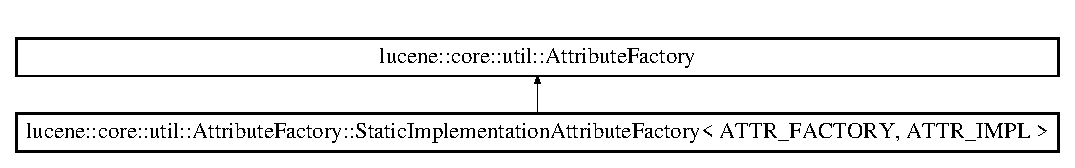
\includegraphics[height=1.815235cm]{classlucene_1_1core_1_1util_1_1AttributeFactory_1_1StaticImplementationAttributeFactory}
\end{center}
\end{figure}
\subsection*{Public Member Functions}
\begin{DoxyCompactItemize}
\item 
\mbox{\hyperlink{classlucene_1_1core_1_1util_1_1AttributeFactory_1_1StaticImplementationAttributeFactory_aed1692d943f8a70e46a85a739743ae94}{Static\+Implementation\+Attribute\+Factory}} ()
\item 
virtual \mbox{\hyperlink{classlucene_1_1core_1_1util_1_1AttributeFactory_1_1StaticImplementationAttributeFactory_a5f8394a6ae54e7aed546e0b8f40ce400}{$\sim$\+Static\+Implementation\+Attribute\+Factory}} ()
\item 
\mbox{\hyperlink{classlucene_1_1core_1_1util_1_1AttributeImpl}{Attribute\+Impl}} $\ast$ \mbox{\hyperlink{classlucene_1_1core_1_1util_1_1AttributeFactory_1_1StaticImplementationAttributeFactory_a06466469f2cf37e0ef599e617d415c6a}{Create\+Attribute\+Instance}} (const std\+::type\+\_\+index attr\+\_\+type\+\_\+id) override
\end{DoxyCompactItemize}
\subsection*{Private Attributes}
\begin{DoxyCompactItemize}
\item 
A\+T\+T\+R\+\_\+\+F\+A\+C\+T\+O\+RY \mbox{\hyperlink{classlucene_1_1core_1_1util_1_1AttributeFactory_1_1StaticImplementationAttributeFactory_af9df5d3fee613815d29578b1c297d8e5}{delegate}}
\end{DoxyCompactItemize}
\subsection*{Static Private Attributes}
\begin{DoxyCompactItemize}
\item 
static std\+::unordered\+\_\+set$<$ std\+::type\+\_\+index $>$ \mbox{\hyperlink{classlucene_1_1core_1_1util_1_1AttributeFactory_1_1StaticImplementationAttributeFactory_a8bf6856d9370f3036f27bed2e0fa819a}{D\+E\+F\+A\+U\+L\+T\+\_\+\+A\+T\+T\+R\+\_\+\+T\+Y\+P\+E\+\_\+\+I\+DS}}
\end{DoxyCompactItemize}
\subsection*{Additional Inherited Members}


\subsection{Constructor \& Destructor Documentation}
\mbox{\Hypertarget{classlucene_1_1core_1_1util_1_1AttributeFactory_1_1StaticImplementationAttributeFactory_aed1692d943f8a70e46a85a739743ae94}\label{classlucene_1_1core_1_1util_1_1AttributeFactory_1_1StaticImplementationAttributeFactory_aed1692d943f8a70e46a85a739743ae94}} 
\index{lucene\+::core\+::util\+::\+Attribute\+Factory\+::\+Static\+Implementation\+Attribute\+Factory@{lucene\+::core\+::util\+::\+Attribute\+Factory\+::\+Static\+Implementation\+Attribute\+Factory}!Static\+Implementation\+Attribute\+Factory@{Static\+Implementation\+Attribute\+Factory}}
\index{Static\+Implementation\+Attribute\+Factory@{Static\+Implementation\+Attribute\+Factory}!lucene\+::core\+::util\+::\+Attribute\+Factory\+::\+Static\+Implementation\+Attribute\+Factory@{lucene\+::core\+::util\+::\+Attribute\+Factory\+::\+Static\+Implementation\+Attribute\+Factory}}
\subsubsection{\texorpdfstring{Static\+Implementation\+Attribute\+Factory()}{StaticImplementationAttributeFactory()}}
{\footnotesize\ttfamily template$<$typename A\+T\+T\+R\+\_\+\+F\+A\+C\+T\+O\+RY , typename A\+T\+T\+R\+\_\+\+I\+M\+PL $>$ \\
\mbox{\hyperlink{classlucene_1_1core_1_1util_1_1AttributeFactory_1_1StaticImplementationAttributeFactory}{lucene\+::core\+::util\+::\+Attribute\+Factory\+::\+Static\+Implementation\+Attribute\+Factory}}$<$ A\+T\+T\+R\+\_\+\+F\+A\+C\+T\+O\+RY, A\+T\+T\+R\+\_\+\+I\+M\+PL $>$\+::\mbox{\hyperlink{classlucene_1_1core_1_1util_1_1AttributeFactory_1_1StaticImplementationAttributeFactory}{Static\+Implementation\+Attribute\+Factory}} (\begin{DoxyParamCaption}{ }\end{DoxyParamCaption})\hspace{0.3cm}{\ttfamily [inline]}}

\mbox{\Hypertarget{classlucene_1_1core_1_1util_1_1AttributeFactory_1_1StaticImplementationAttributeFactory_a5f8394a6ae54e7aed546e0b8f40ce400}\label{classlucene_1_1core_1_1util_1_1AttributeFactory_1_1StaticImplementationAttributeFactory_a5f8394a6ae54e7aed546e0b8f40ce400}} 
\index{lucene\+::core\+::util\+::\+Attribute\+Factory\+::\+Static\+Implementation\+Attribute\+Factory@{lucene\+::core\+::util\+::\+Attribute\+Factory\+::\+Static\+Implementation\+Attribute\+Factory}!````~Static\+Implementation\+Attribute\+Factory@{$\sim$\+Static\+Implementation\+Attribute\+Factory}}
\index{````~Static\+Implementation\+Attribute\+Factory@{$\sim$\+Static\+Implementation\+Attribute\+Factory}!lucene\+::core\+::util\+::\+Attribute\+Factory\+::\+Static\+Implementation\+Attribute\+Factory@{lucene\+::core\+::util\+::\+Attribute\+Factory\+::\+Static\+Implementation\+Attribute\+Factory}}
\subsubsection{\texorpdfstring{$\sim$\+Static\+Implementation\+Attribute\+Factory()}{~StaticImplementationAttributeFactory()}}
{\footnotesize\ttfamily template$<$typename A\+T\+T\+R\+\_\+\+F\+A\+C\+T\+O\+RY , typename A\+T\+T\+R\+\_\+\+I\+M\+PL $>$ \\
virtual \mbox{\hyperlink{classlucene_1_1core_1_1util_1_1AttributeFactory_1_1StaticImplementationAttributeFactory}{lucene\+::core\+::util\+::\+Attribute\+Factory\+::\+Static\+Implementation\+Attribute\+Factory}}$<$ A\+T\+T\+R\+\_\+\+F\+A\+C\+T\+O\+RY, A\+T\+T\+R\+\_\+\+I\+M\+PL $>$\+::$\sim$\mbox{\hyperlink{classlucene_1_1core_1_1util_1_1AttributeFactory_1_1StaticImplementationAttributeFactory}{Static\+Implementation\+Attribute\+Factory}} (\begin{DoxyParamCaption}{ }\end{DoxyParamCaption})\hspace{0.3cm}{\ttfamily [inline]}, {\ttfamily [virtual]}}



\subsection{Member Function Documentation}
\mbox{\Hypertarget{classlucene_1_1core_1_1util_1_1AttributeFactory_1_1StaticImplementationAttributeFactory_a06466469f2cf37e0ef599e617d415c6a}\label{classlucene_1_1core_1_1util_1_1AttributeFactory_1_1StaticImplementationAttributeFactory_a06466469f2cf37e0ef599e617d415c6a}} 
\index{lucene\+::core\+::util\+::\+Attribute\+Factory\+::\+Static\+Implementation\+Attribute\+Factory@{lucene\+::core\+::util\+::\+Attribute\+Factory\+::\+Static\+Implementation\+Attribute\+Factory}!Create\+Attribute\+Instance@{Create\+Attribute\+Instance}}
\index{Create\+Attribute\+Instance@{Create\+Attribute\+Instance}!lucene\+::core\+::util\+::\+Attribute\+Factory\+::\+Static\+Implementation\+Attribute\+Factory@{lucene\+::core\+::util\+::\+Attribute\+Factory\+::\+Static\+Implementation\+Attribute\+Factory}}
\subsubsection{\texorpdfstring{Create\+Attribute\+Instance()}{CreateAttributeInstance()}}
{\footnotesize\ttfamily template$<$typename A\+T\+T\+R\+\_\+\+F\+A\+C\+T\+O\+RY , typename A\+T\+T\+R\+\_\+\+I\+M\+PL $>$ \\
\mbox{\hyperlink{classlucene_1_1core_1_1util_1_1AttributeImpl}{Attribute\+Impl}}$\ast$ \mbox{\hyperlink{classlucene_1_1core_1_1util_1_1AttributeFactory_1_1StaticImplementationAttributeFactory}{lucene\+::core\+::util\+::\+Attribute\+Factory\+::\+Static\+Implementation\+Attribute\+Factory}}$<$ A\+T\+T\+R\+\_\+\+F\+A\+C\+T\+O\+RY, A\+T\+T\+R\+\_\+\+I\+M\+PL $>$\+::Create\+Attribute\+Instance (\begin{DoxyParamCaption}\item[{const std\+::type\+\_\+index}]{attr\+\_\+type\+\_\+id }\end{DoxyParamCaption})\hspace{0.3cm}{\ttfamily [inline]}, {\ttfamily [override]}, {\ttfamily [virtual]}}



Implements \mbox{\hyperlink{classlucene_1_1core_1_1util_1_1AttributeFactory_a88ccb9965ed78099379eaf9b1256abf3}{lucene\+::core\+::util\+::\+Attribute\+Factory}}.



\subsection{Member Data Documentation}
\mbox{\Hypertarget{classlucene_1_1core_1_1util_1_1AttributeFactory_1_1StaticImplementationAttributeFactory_a8bf6856d9370f3036f27bed2e0fa819a}\label{classlucene_1_1core_1_1util_1_1AttributeFactory_1_1StaticImplementationAttributeFactory_a8bf6856d9370f3036f27bed2e0fa819a}} 
\index{lucene\+::core\+::util\+::\+Attribute\+Factory\+::\+Static\+Implementation\+Attribute\+Factory@{lucene\+::core\+::util\+::\+Attribute\+Factory\+::\+Static\+Implementation\+Attribute\+Factory}!D\+E\+F\+A\+U\+L\+T\+\_\+\+A\+T\+T\+R\+\_\+\+T\+Y\+P\+E\+\_\+\+I\+DS@{D\+E\+F\+A\+U\+L\+T\+\_\+\+A\+T\+T\+R\+\_\+\+T\+Y\+P\+E\+\_\+\+I\+DS}}
\index{D\+E\+F\+A\+U\+L\+T\+\_\+\+A\+T\+T\+R\+\_\+\+T\+Y\+P\+E\+\_\+\+I\+DS@{D\+E\+F\+A\+U\+L\+T\+\_\+\+A\+T\+T\+R\+\_\+\+T\+Y\+P\+E\+\_\+\+I\+DS}!lucene\+::core\+::util\+::\+Attribute\+Factory\+::\+Static\+Implementation\+Attribute\+Factory@{lucene\+::core\+::util\+::\+Attribute\+Factory\+::\+Static\+Implementation\+Attribute\+Factory}}
\subsubsection{\texorpdfstring{D\+E\+F\+A\+U\+L\+T\+\_\+\+A\+T\+T\+R\+\_\+\+T\+Y\+P\+E\+\_\+\+I\+DS}{DEFAULT\_ATTR\_TYPE\_IDS}}
{\footnotesize\ttfamily template$<$typename A\+T\+T\+R\+\_\+\+F\+A\+C\+T\+O\+RY , typename A\+T\+T\+R\+\_\+\+I\+M\+PL $>$ \\
std\+::unordered\+\_\+set$<$ std\+::type\+\_\+index $>$ \mbox{\hyperlink{classlucene_1_1core_1_1util_1_1AttributeFactory_1_1StaticImplementationAttributeFactory}{lucene\+::core\+::util\+::\+Attribute\+Factory\+::\+Static\+Implementation\+Attribute\+Factory}}$<$ A\+T\+T\+R\+\_\+\+F\+A\+C\+T\+O\+RY, A\+T\+T\+R\+\_\+\+I\+M\+PL $>$\+::D\+E\+F\+A\+U\+L\+T\+\_\+\+A\+T\+T\+R\+\_\+\+T\+Y\+P\+E\+\_\+\+I\+DS\hspace{0.3cm}{\ttfamily [static]}, {\ttfamily [private]}}

{\bfseries Initial value\+:}
\begin{DoxyCode}
\DoxyCodeLine{= []() \{}
\DoxyCodeLine{  std::unordered\_set<std::type\_index>}
\DoxyCodeLine{  ret(\mbox{\hyperlink{classlucene_1_1core_1_1util_1_1AttributeFactory_a5247e47d95ce30862a15e66ce2266d04}{AttributeFactory::ATTR\_IMPL\_TABLE}}.size());}
\DoxyCodeLine{}
\DoxyCodeLine{  \textcolor{keywordflow}{for} (\textcolor{keyword}{const} \textcolor{keyword}{auto}\& p : \mbox{\hyperlink{classlucene_1_1core_1_1util_1_1AttributeFactory_a5247e47d95ce30862a15e66ce2266d04}{AttributeFactory::ATTR\_IMPL\_TABLE}}) \{}
\DoxyCodeLine{    ret.insert(p.first);}
\DoxyCodeLine{  \}}
\DoxyCodeLine{  \textcolor{keywordflow}{return} ret;}
\DoxyCodeLine{\}()}
\end{DoxyCode}
\mbox{\Hypertarget{classlucene_1_1core_1_1util_1_1AttributeFactory_1_1StaticImplementationAttributeFactory_af9df5d3fee613815d29578b1c297d8e5}\label{classlucene_1_1core_1_1util_1_1AttributeFactory_1_1StaticImplementationAttributeFactory_af9df5d3fee613815d29578b1c297d8e5}} 
\index{lucene\+::core\+::util\+::\+Attribute\+Factory\+::\+Static\+Implementation\+Attribute\+Factory@{lucene\+::core\+::util\+::\+Attribute\+Factory\+::\+Static\+Implementation\+Attribute\+Factory}!delegate@{delegate}}
\index{delegate@{delegate}!lucene\+::core\+::util\+::\+Attribute\+Factory\+::\+Static\+Implementation\+Attribute\+Factory@{lucene\+::core\+::util\+::\+Attribute\+Factory\+::\+Static\+Implementation\+Attribute\+Factory}}
\subsubsection{\texorpdfstring{delegate}{delegate}}
{\footnotesize\ttfamily template$<$typename A\+T\+T\+R\+\_\+\+F\+A\+C\+T\+O\+RY , typename A\+T\+T\+R\+\_\+\+I\+M\+PL $>$ \\
A\+T\+T\+R\+\_\+\+F\+A\+C\+T\+O\+RY \mbox{\hyperlink{classlucene_1_1core_1_1util_1_1AttributeFactory_1_1StaticImplementationAttributeFactory}{lucene\+::core\+::util\+::\+Attribute\+Factory\+::\+Static\+Implementation\+Attribute\+Factory}}$<$ A\+T\+T\+R\+\_\+\+F\+A\+C\+T\+O\+RY, A\+T\+T\+R\+\_\+\+I\+M\+PL $>$\+::delegate\hspace{0.3cm}{\ttfamily [private]}}



The documentation for this class was generated from the following file\+:\begin{DoxyCompactItemize}
\item 
Util/\mbox{\hyperlink{Util_2Attribute_8h}{Attribute.\+h}}\end{DoxyCompactItemize}

\hypertarget{classlucene_1_1core_1_1analysis_1_1StopFilter}{}\section{lucene\+:\+:core\+:\+:analysis\+:\+:Stop\+Filter Class Reference}
\label{classlucene_1_1core_1_1analysis_1_1StopFilter}\index{lucene\+::core\+::analysis\+::\+Stop\+Filter@{lucene\+::core\+::analysis\+::\+Stop\+Filter}}


{\ttfamily \#include $<$Token\+Stream.\+h$>$}

Inheritance diagram for lucene\+:\+:core\+:\+:analysis\+:\+:Stop\+Filter\+:\begin{figure}[H]
\begin{center}
\leavevmode
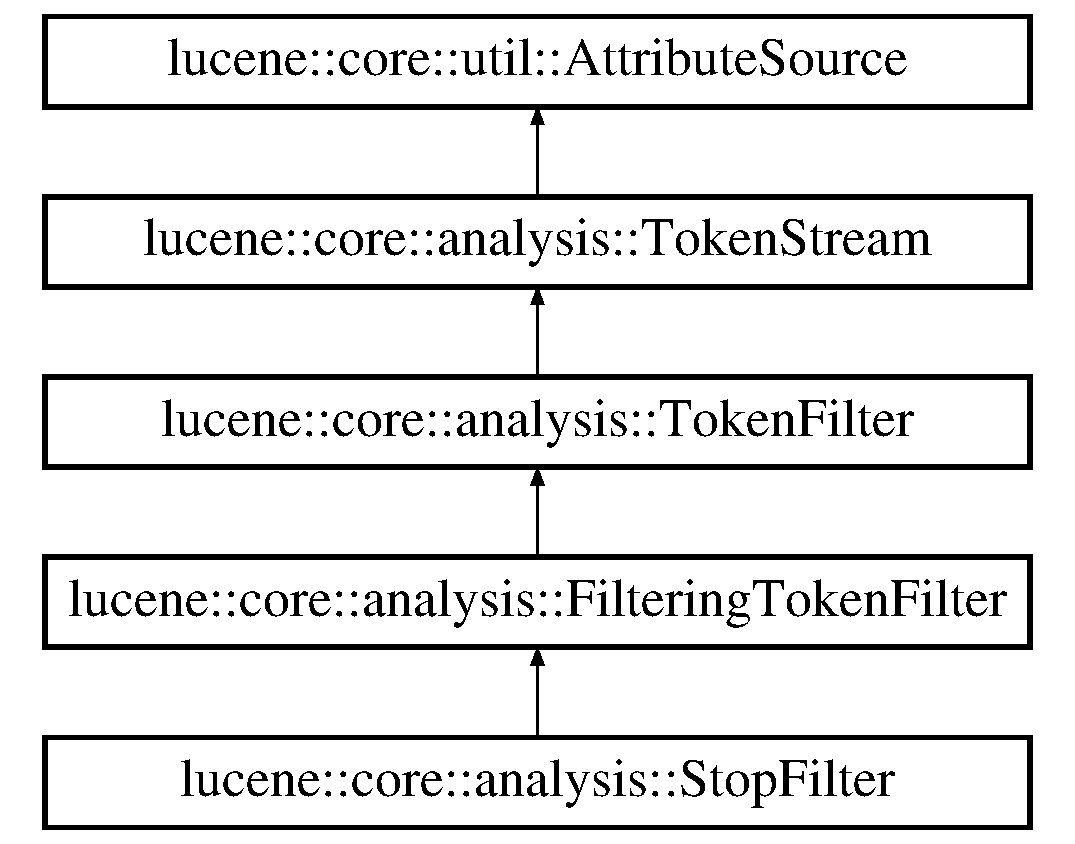
\includegraphics[height=5.000000cm]{classlucene_1_1core_1_1analysis_1_1StopFilter}
\end{center}
\end{figure}
\subsection*{Public Member Functions}
\begin{DoxyCompactItemize}
\item 
\mbox{\hyperlink{classlucene_1_1core_1_1analysis_1_1StopFilter_ac7db0ba3cf53a65d25442b1a2b290156}{Stop\+Filter}} (\mbox{\hyperlink{classlucene_1_1core_1_1analysis_1_1TokenStream}{Token\+Stream}} $\ast$in, \mbox{\hyperlink{classlucene_1_1core_1_1analysis_1_1characterutil_1_1CharSet}{characterutil\+::\+Char\+Set}} \&\mbox{\hyperlink{classlucene_1_1core_1_1analysis_1_1StopFilter_ace188f785bcebdc0f18a73116da1afd0}{stop\+\_\+words}})
\item 
\mbox{\hyperlink{classlucene_1_1core_1_1analysis_1_1StopFilter_a86879713f0135ab08a996e716f87aadb}{Stop\+Filter}} (\mbox{\hyperlink{classlucene_1_1core_1_1analysis_1_1TokenStream}{Token\+Stream}} $\ast$in, \mbox{\hyperlink{classlucene_1_1core_1_1analysis_1_1characterutil_1_1CharSet}{characterutil\+::\+Char\+Set}} \&\&\mbox{\hyperlink{classlucene_1_1core_1_1analysis_1_1StopFilter_ace188f785bcebdc0f18a73116da1afd0}{stop\+\_\+words}})
\item 
\mbox{\hyperlink{classlucene_1_1core_1_1analysis_1_1StopFilter_a49efaebf256d312e5fef43b7322c1e52}{Stop\+Filter}} (std\+::shared\+\_\+ptr$<$ \mbox{\hyperlink{classlucene_1_1core_1_1analysis_1_1TokenStream}{Token\+Stream}} $>$ in, \mbox{\hyperlink{classlucene_1_1core_1_1analysis_1_1characterutil_1_1CharSet}{characterutil\+::\+Char\+Set}} \&\mbox{\hyperlink{classlucene_1_1core_1_1analysis_1_1StopFilter_ace188f785bcebdc0f18a73116da1afd0}{stop\+\_\+words}})
\item 
\mbox{\hyperlink{classlucene_1_1core_1_1analysis_1_1StopFilter_ae2465c47647c009fd479ada9a7d2cb85}{Stop\+Filter}} (std\+::shared\+\_\+ptr$<$ \mbox{\hyperlink{classlucene_1_1core_1_1analysis_1_1TokenStream}{Token\+Stream}} $>$ in, \mbox{\hyperlink{classlucene_1_1core_1_1analysis_1_1characterutil_1_1CharSet}{characterutil\+::\+Char\+Set}} \&\&\mbox{\hyperlink{classlucene_1_1core_1_1analysis_1_1StopFilter_ace188f785bcebdc0f18a73116da1afd0}{stop\+\_\+words}})
\item 
virtual \mbox{\hyperlink{classlucene_1_1core_1_1analysis_1_1StopFilter_a78c7542a5cc8588d60babac01fa27eaf}{$\sim$\+Stop\+Filter}} ()
\end{DoxyCompactItemize}
\subsection*{Static Public Member Functions}
\begin{DoxyCompactItemize}
\item 
static \mbox{\hyperlink{classlucene_1_1core_1_1analysis_1_1characterutil_1_1CharSet}{characterutil\+::\+Char\+Set}} \mbox{\hyperlink{classlucene_1_1core_1_1analysis_1_1StopFilter_ac27f79322c5118e5ac408e250203e17e}{Make\+Stop\+Set}} (std\+::vector$<$ std\+::string $>$ \&\mbox{\hyperlink{classlucene_1_1core_1_1analysis_1_1StopFilter_ace188f785bcebdc0f18a73116da1afd0}{stop\+\_\+words}}, bool ignore\+\_\+case=false)
\end{DoxyCompactItemize}
\subsection*{Protected Member Functions}
\begin{DoxyCompactItemize}
\item 
bool \mbox{\hyperlink{classlucene_1_1core_1_1analysis_1_1StopFilter_af05114955fb7b1deb340a7fe1e07735e}{Accept}} () override
\end{DoxyCompactItemize}
\subsection*{Private Attributes}
\begin{DoxyCompactItemize}
\item 
\mbox{\hyperlink{classlucene_1_1core_1_1analysis_1_1characterutil_1_1CharSet}{characterutil\+::\+Char\+Set}} \mbox{\hyperlink{classlucene_1_1core_1_1analysis_1_1StopFilter_ace188f785bcebdc0f18a73116da1afd0}{stop\+\_\+words}}
\item 
std\+::shared\+\_\+ptr$<$ \mbox{\hyperlink{classlucene_1_1core_1_1analysis_1_1tokenattributes_1_1CharTermAttribute}{tokenattributes\+::\+Char\+Term\+Attribute}} $>$ \mbox{\hyperlink{classlucene_1_1core_1_1analysis_1_1StopFilter_aa625432d1343f5a67be010bde710a986}{term\+\_\+att}}
\end{DoxyCompactItemize}
\subsection*{Additional Inherited Members}


\subsection{Constructor \& Destructor Documentation}
\mbox{\Hypertarget{classlucene_1_1core_1_1analysis_1_1StopFilter_ac7db0ba3cf53a65d25442b1a2b290156}\label{classlucene_1_1core_1_1analysis_1_1StopFilter_ac7db0ba3cf53a65d25442b1a2b290156}} 
\index{lucene\+::core\+::analysis\+::\+Stop\+Filter@{lucene\+::core\+::analysis\+::\+Stop\+Filter}!Stop\+Filter@{Stop\+Filter}}
\index{Stop\+Filter@{Stop\+Filter}!lucene\+::core\+::analysis\+::\+Stop\+Filter@{lucene\+::core\+::analysis\+::\+Stop\+Filter}}
\subsubsection{\texorpdfstring{Stop\+Filter()}{StopFilter()}\hspace{0.1cm}{\footnotesize\ttfamily [1/4]}}
{\footnotesize\ttfamily Stop\+Filter\+::\+Stop\+Filter (\begin{DoxyParamCaption}\item[{\mbox{\hyperlink{classlucene_1_1core_1_1analysis_1_1TokenStream}{Token\+Stream}} $\ast$}]{in,  }\item[{\mbox{\hyperlink{classlucene_1_1core_1_1analysis_1_1characterutil_1_1CharSet}{characterutil\+::\+Char\+Set}} \&}]{stop\+\_\+words }\end{DoxyParamCaption})}

\mbox{\hyperlink{classlucene_1_1core_1_1analysis_1_1StopFilter}{Stop\+Filter}} \mbox{\Hypertarget{classlucene_1_1core_1_1analysis_1_1StopFilter_a86879713f0135ab08a996e716f87aadb}\label{classlucene_1_1core_1_1analysis_1_1StopFilter_a86879713f0135ab08a996e716f87aadb}} 
\index{lucene\+::core\+::analysis\+::\+Stop\+Filter@{lucene\+::core\+::analysis\+::\+Stop\+Filter}!Stop\+Filter@{Stop\+Filter}}
\index{Stop\+Filter@{Stop\+Filter}!lucene\+::core\+::analysis\+::\+Stop\+Filter@{lucene\+::core\+::analysis\+::\+Stop\+Filter}}
\subsubsection{\texorpdfstring{Stop\+Filter()}{StopFilter()}\hspace{0.1cm}{\footnotesize\ttfamily [2/4]}}
{\footnotesize\ttfamily Stop\+Filter\+::\+Stop\+Filter (\begin{DoxyParamCaption}\item[{\mbox{\hyperlink{classlucene_1_1core_1_1analysis_1_1TokenStream}{Token\+Stream}} $\ast$}]{in,  }\item[{\mbox{\hyperlink{classlucene_1_1core_1_1analysis_1_1characterutil_1_1CharSet}{characterutil\+::\+Char\+Set}} \&\&}]{stop\+\_\+words }\end{DoxyParamCaption})}

\mbox{\Hypertarget{classlucene_1_1core_1_1analysis_1_1StopFilter_a49efaebf256d312e5fef43b7322c1e52}\label{classlucene_1_1core_1_1analysis_1_1StopFilter_a49efaebf256d312e5fef43b7322c1e52}} 
\index{lucene\+::core\+::analysis\+::\+Stop\+Filter@{lucene\+::core\+::analysis\+::\+Stop\+Filter}!Stop\+Filter@{Stop\+Filter}}
\index{Stop\+Filter@{Stop\+Filter}!lucene\+::core\+::analysis\+::\+Stop\+Filter@{lucene\+::core\+::analysis\+::\+Stop\+Filter}}
\subsubsection{\texorpdfstring{Stop\+Filter()}{StopFilter()}\hspace{0.1cm}{\footnotesize\ttfamily [3/4]}}
{\footnotesize\ttfamily lucene\+::core\+::analysis\+::\+Stop\+Filter\+::\+Stop\+Filter (\begin{DoxyParamCaption}\item[{std\+::shared\+\_\+ptr$<$ \mbox{\hyperlink{classlucene_1_1core_1_1analysis_1_1TokenStream}{Token\+Stream}} $>$}]{in,  }\item[{\mbox{\hyperlink{classlucene_1_1core_1_1analysis_1_1characterutil_1_1CharSet}{characterutil\+::\+Char\+Set}} \&}]{stop\+\_\+words }\end{DoxyParamCaption})}

\mbox{\Hypertarget{classlucene_1_1core_1_1analysis_1_1StopFilter_ae2465c47647c009fd479ada9a7d2cb85}\label{classlucene_1_1core_1_1analysis_1_1StopFilter_ae2465c47647c009fd479ada9a7d2cb85}} 
\index{lucene\+::core\+::analysis\+::\+Stop\+Filter@{lucene\+::core\+::analysis\+::\+Stop\+Filter}!Stop\+Filter@{Stop\+Filter}}
\index{Stop\+Filter@{Stop\+Filter}!lucene\+::core\+::analysis\+::\+Stop\+Filter@{lucene\+::core\+::analysis\+::\+Stop\+Filter}}
\subsubsection{\texorpdfstring{Stop\+Filter()}{StopFilter()}\hspace{0.1cm}{\footnotesize\ttfamily [4/4]}}
{\footnotesize\ttfamily lucene\+::core\+::analysis\+::\+Stop\+Filter\+::\+Stop\+Filter (\begin{DoxyParamCaption}\item[{std\+::shared\+\_\+ptr$<$ \mbox{\hyperlink{classlucene_1_1core_1_1analysis_1_1TokenStream}{Token\+Stream}} $>$}]{in,  }\item[{\mbox{\hyperlink{classlucene_1_1core_1_1analysis_1_1characterutil_1_1CharSet}{characterutil\+::\+Char\+Set}} \&\&}]{stop\+\_\+words }\end{DoxyParamCaption})}

\mbox{\Hypertarget{classlucene_1_1core_1_1analysis_1_1StopFilter_a78c7542a5cc8588d60babac01fa27eaf}\label{classlucene_1_1core_1_1analysis_1_1StopFilter_a78c7542a5cc8588d60babac01fa27eaf}} 
\index{lucene\+::core\+::analysis\+::\+Stop\+Filter@{lucene\+::core\+::analysis\+::\+Stop\+Filter}!````~Stop\+Filter@{$\sim$\+Stop\+Filter}}
\index{````~Stop\+Filter@{$\sim$\+Stop\+Filter}!lucene\+::core\+::analysis\+::\+Stop\+Filter@{lucene\+::core\+::analysis\+::\+Stop\+Filter}}
\subsubsection{\texorpdfstring{$\sim$\+Stop\+Filter()}{~StopFilter()}}
{\footnotesize\ttfamily Stop\+Filter\+::$\sim$\+Stop\+Filter (\begin{DoxyParamCaption}{ }\end{DoxyParamCaption})\hspace{0.3cm}{\ttfamily [virtual]}}



\subsection{Member Function Documentation}
\mbox{\Hypertarget{classlucene_1_1core_1_1analysis_1_1StopFilter_af05114955fb7b1deb340a7fe1e07735e}\label{classlucene_1_1core_1_1analysis_1_1StopFilter_af05114955fb7b1deb340a7fe1e07735e}} 
\index{lucene\+::core\+::analysis\+::\+Stop\+Filter@{lucene\+::core\+::analysis\+::\+Stop\+Filter}!Accept@{Accept}}
\index{Accept@{Accept}!lucene\+::core\+::analysis\+::\+Stop\+Filter@{lucene\+::core\+::analysis\+::\+Stop\+Filter}}
\subsubsection{\texorpdfstring{Accept()}{Accept()}}
{\footnotesize\ttfamily bool Stop\+Filter\+::\+Accept (\begin{DoxyParamCaption}{ }\end{DoxyParamCaption})\hspace{0.3cm}{\ttfamily [override]}, {\ttfamily [protected]}, {\ttfamily [virtual]}}



Implements \mbox{\hyperlink{classlucene_1_1core_1_1analysis_1_1FilteringTokenFilter_a4a2fb2dd2d3bda8eb6cd0d5b14a4ab92}{lucene\+::core\+::analysis\+::\+Filtering\+Token\+Filter}}.

\mbox{\Hypertarget{classlucene_1_1core_1_1analysis_1_1StopFilter_ac27f79322c5118e5ac408e250203e17e}\label{classlucene_1_1core_1_1analysis_1_1StopFilter_ac27f79322c5118e5ac408e250203e17e}} 
\index{lucene\+::core\+::analysis\+::\+Stop\+Filter@{lucene\+::core\+::analysis\+::\+Stop\+Filter}!Make\+Stop\+Set@{Make\+Stop\+Set}}
\index{Make\+Stop\+Set@{Make\+Stop\+Set}!lucene\+::core\+::analysis\+::\+Stop\+Filter@{lucene\+::core\+::analysis\+::\+Stop\+Filter}}
\subsubsection{\texorpdfstring{Make\+Stop\+Set()}{MakeStopSet()}}
{\footnotesize\ttfamily static \mbox{\hyperlink{classlucene_1_1core_1_1analysis_1_1characterutil_1_1CharSet}{characterutil\+::\+Char\+Set}} lucene\+::core\+::analysis\+::\+Stop\+Filter\+::\+Make\+Stop\+Set (\begin{DoxyParamCaption}\item[{std\+::vector$<$ std\+::string $>$ \&}]{stop\+\_\+words,  }\item[{bool}]{ignore\+\_\+case = {\ttfamily false} }\end{DoxyParamCaption})\hspace{0.3cm}{\ttfamily [static]}}



\subsection{Member Data Documentation}
\mbox{\Hypertarget{classlucene_1_1core_1_1analysis_1_1StopFilter_ace188f785bcebdc0f18a73116da1afd0}\label{classlucene_1_1core_1_1analysis_1_1StopFilter_ace188f785bcebdc0f18a73116da1afd0}} 
\index{lucene\+::core\+::analysis\+::\+Stop\+Filter@{lucene\+::core\+::analysis\+::\+Stop\+Filter}!stop\+\_\+words@{stop\+\_\+words}}
\index{stop\+\_\+words@{stop\+\_\+words}!lucene\+::core\+::analysis\+::\+Stop\+Filter@{lucene\+::core\+::analysis\+::\+Stop\+Filter}}
\subsubsection{\texorpdfstring{stop\+\_\+words}{stop\_words}}
{\footnotesize\ttfamily \mbox{\hyperlink{classlucene_1_1core_1_1analysis_1_1characterutil_1_1CharSet}{characterutil\+::\+Char\+Set}} lucene\+::core\+::analysis\+::\+Stop\+Filter\+::stop\+\_\+words\hspace{0.3cm}{\ttfamily [private]}}

\mbox{\Hypertarget{classlucene_1_1core_1_1analysis_1_1StopFilter_aa625432d1343f5a67be010bde710a986}\label{classlucene_1_1core_1_1analysis_1_1StopFilter_aa625432d1343f5a67be010bde710a986}} 
\index{lucene\+::core\+::analysis\+::\+Stop\+Filter@{lucene\+::core\+::analysis\+::\+Stop\+Filter}!term\+\_\+att@{term\+\_\+att}}
\index{term\+\_\+att@{term\+\_\+att}!lucene\+::core\+::analysis\+::\+Stop\+Filter@{lucene\+::core\+::analysis\+::\+Stop\+Filter}}
\subsubsection{\texorpdfstring{term\+\_\+att}{term\_att}}
{\footnotesize\ttfamily std\+::shared\+\_\+ptr$<$\mbox{\hyperlink{classlucene_1_1core_1_1analysis_1_1tokenattributes_1_1CharTermAttribute}{tokenattributes\+::\+Char\+Term\+Attribute}}$>$ lucene\+::core\+::analysis\+::\+Stop\+Filter\+::term\+\_\+att\hspace{0.3cm}{\ttfamily [private]}}



The documentation for this class was generated from the following files\+:\begin{DoxyCompactItemize}
\item 
Analysis/\mbox{\hyperlink{TokenStream_8h}{Token\+Stream.\+h}}\item 
Analysis/\mbox{\hyperlink{TokenStream_8cpp}{Token\+Stream.\+cpp}}\end{DoxyCompactItemize}

\hypertarget{classlucene_1_1core_1_1analysis_1_1StopwordAnalyzerBase}{}\section{lucene\+:\+:core\+:\+:analysis\+:\+:Stopword\+Analyzer\+Base Class Reference}
\label{classlucene_1_1core_1_1analysis_1_1StopwordAnalyzerBase}\index{lucene\+::core\+::analysis\+::\+Stopword\+Analyzer\+Base@{lucene\+::core\+::analysis\+::\+Stopword\+Analyzer\+Base}}


{\ttfamily \#include $<$Analyzer.\+h$>$}

Inheritance diagram for lucene\+:\+:core\+:\+:analysis\+:\+:Stopword\+Analyzer\+Base\+:\begin{figure}[H]
\begin{center}
\leavevmode
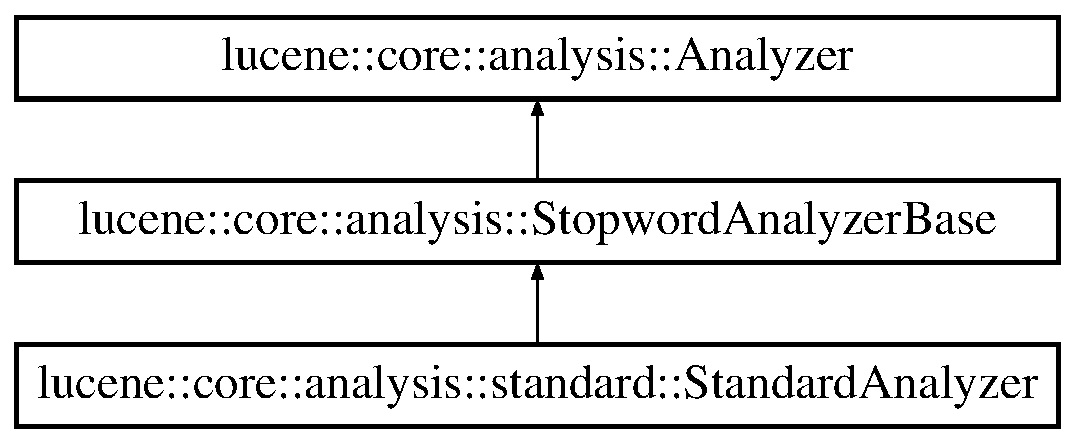
\includegraphics[height=3.000000cm]{classlucene_1_1core_1_1analysis_1_1StopwordAnalyzerBase}
\end{center}
\end{figure}
\subsection*{Public Member Functions}
\begin{DoxyCompactItemize}
\item 
\mbox{\hyperlink{classlucene_1_1core_1_1analysis_1_1characterutil_1_1CharSet}{characterutil\+::\+Char\+Set}} \& \mbox{\hyperlink{classlucene_1_1core_1_1analysis_1_1StopwordAnalyzerBase_aaa0f8763081ba7e41278a03ee5622980}{Get\+Stop\+Words}} ()
\end{DoxyCompactItemize}
\subsection*{Protected Member Functions}
\begin{DoxyCompactItemize}
\item 
\mbox{\hyperlink{classlucene_1_1core_1_1analysis_1_1StopwordAnalyzerBase_a07e1b2362b8ac3776cf456250884f898}{Stopword\+Analyzer\+Base}} (\mbox{\hyperlink{ZlibCrc32_8h_a2c212835823e3c54a8ab6d95c652660e}{const}} \mbox{\hyperlink{classlucene_1_1core_1_1analysis_1_1characterutil_1_1CharSet}{characterutil\+::\+Char\+Set}} \&\mbox{\hyperlink{classlucene_1_1core_1_1analysis_1_1StopwordAnalyzerBase_a12ceda198e84aabe357ccd7b28e66d07}{stop\+\_\+words}})
\item 
\mbox{\hyperlink{classlucene_1_1core_1_1analysis_1_1StopwordAnalyzerBase_ab15b0a23b58e1d09b2d65338349f0260}{Stopword\+Analyzer\+Base}} (\mbox{\hyperlink{classlucene_1_1core_1_1analysis_1_1characterutil_1_1CharSet}{characterutil\+::\+Char\+Set}} \&\&\mbox{\hyperlink{classlucene_1_1core_1_1analysis_1_1StopwordAnalyzerBase_a12ceda198e84aabe357ccd7b28e66d07}{stop\+\_\+words}})
\item 
\mbox{\hyperlink{classlucene_1_1core_1_1analysis_1_1StopwordAnalyzerBase_a94f2df7bf83363d5690e925c3140157d}{Stopword\+Analyzer\+Base}} ()
\item 
virtual \mbox{\hyperlink{classlucene_1_1core_1_1analysis_1_1StopwordAnalyzerBase_a464b01561952e4244b31df0a61045d63}{$\sim$\+Stopword\+Analyzer\+Base}} ()
\end{DoxyCompactItemize}
\subsection*{Static Protected Member Functions}
\begin{DoxyCompactItemize}
\item 
static \mbox{\hyperlink{classlucene_1_1core_1_1analysis_1_1characterutil_1_1CharSet}{characterutil\+::\+Char\+Set}} \mbox{\hyperlink{classlucene_1_1core_1_1analysis_1_1StopwordAnalyzerBase_a72330e7251da134ad13afdf181c1f04a}{Load\+Stop\+Word\+Set}} (\mbox{\hyperlink{ZlibCrc32_8h_a2c212835823e3c54a8ab6d95c652660e}{const}} std\+::string \&path)
\item 
static \mbox{\hyperlink{classlucene_1_1core_1_1analysis_1_1characterutil_1_1CharSet}{characterutil\+::\+Char\+Set}} \mbox{\hyperlink{classlucene_1_1core_1_1analysis_1_1StopwordAnalyzerBase_ab768bf79e306a74d72ecfea48080018f}{Load\+Stop\+Word\+Set}} (\mbox{\hyperlink{ZlibCrc32_8h_a2c212835823e3c54a8ab6d95c652660e}{const}} \mbox{\hyperlink{classlucene_1_1core_1_1analysis_1_1Reader}{Reader}} \&reader)
\end{DoxyCompactItemize}
\subsection*{Protected Attributes}
\begin{DoxyCompactItemize}
\item 
\mbox{\hyperlink{classlucene_1_1core_1_1analysis_1_1characterutil_1_1CharSet}{characterutil\+::\+Char\+Set}} \mbox{\hyperlink{classlucene_1_1core_1_1analysis_1_1StopwordAnalyzerBase_a12ceda198e84aabe357ccd7b28e66d07}{stop\+\_\+words}}
\end{DoxyCompactItemize}


\subsection{Constructor \& Destructor Documentation}
\mbox{\Hypertarget{classlucene_1_1core_1_1analysis_1_1StopwordAnalyzerBase_a07e1b2362b8ac3776cf456250884f898}\label{classlucene_1_1core_1_1analysis_1_1StopwordAnalyzerBase_a07e1b2362b8ac3776cf456250884f898}} 
\index{lucene\+::core\+::analysis\+::\+Stopword\+Analyzer\+Base@{lucene\+::core\+::analysis\+::\+Stopword\+Analyzer\+Base}!Stopword\+Analyzer\+Base@{Stopword\+Analyzer\+Base}}
\index{Stopword\+Analyzer\+Base@{Stopword\+Analyzer\+Base}!lucene\+::core\+::analysis\+::\+Stopword\+Analyzer\+Base@{lucene\+::core\+::analysis\+::\+Stopword\+Analyzer\+Base}}
\subsubsection{\texorpdfstring{Stopword\+Analyzer\+Base()}{StopwordAnalyzerBase()}\hspace{0.1cm}{\footnotesize\ttfamily [1/3]}}
{\footnotesize\ttfamily Stopword\+Analyzer\+Base\+::\+Stopword\+Analyzer\+Base (\begin{DoxyParamCaption}\item[{\mbox{\hyperlink{ZlibCrc32_8h_a2c212835823e3c54a8ab6d95c652660e}{const}} \mbox{\hyperlink{classlucene_1_1core_1_1analysis_1_1characterutil_1_1CharSet}{characterutil\+::\+Char\+Set}} \&}]{stop\+\_\+words }\end{DoxyParamCaption})\hspace{0.3cm}{\ttfamily [explicit]}, {\ttfamily [protected]}}

\mbox{\Hypertarget{classlucene_1_1core_1_1analysis_1_1StopwordAnalyzerBase_ab15b0a23b58e1d09b2d65338349f0260}\label{classlucene_1_1core_1_1analysis_1_1StopwordAnalyzerBase_ab15b0a23b58e1d09b2d65338349f0260}} 
\index{lucene\+::core\+::analysis\+::\+Stopword\+Analyzer\+Base@{lucene\+::core\+::analysis\+::\+Stopword\+Analyzer\+Base}!Stopword\+Analyzer\+Base@{Stopword\+Analyzer\+Base}}
\index{Stopword\+Analyzer\+Base@{Stopword\+Analyzer\+Base}!lucene\+::core\+::analysis\+::\+Stopword\+Analyzer\+Base@{lucene\+::core\+::analysis\+::\+Stopword\+Analyzer\+Base}}
\subsubsection{\texorpdfstring{Stopword\+Analyzer\+Base()}{StopwordAnalyzerBase()}\hspace{0.1cm}{\footnotesize\ttfamily [2/3]}}
{\footnotesize\ttfamily Stopword\+Analyzer\+Base\+::\+Stopword\+Analyzer\+Base (\begin{DoxyParamCaption}\item[{\mbox{\hyperlink{classlucene_1_1core_1_1analysis_1_1characterutil_1_1CharSet}{characterutil\+::\+Char\+Set}} \&\&}]{stop\+\_\+words }\end{DoxyParamCaption})\hspace{0.3cm}{\ttfamily [explicit]}, {\ttfamily [protected]}}

\mbox{\Hypertarget{classlucene_1_1core_1_1analysis_1_1StopwordAnalyzerBase_a94f2df7bf83363d5690e925c3140157d}\label{classlucene_1_1core_1_1analysis_1_1StopwordAnalyzerBase_a94f2df7bf83363d5690e925c3140157d}} 
\index{lucene\+::core\+::analysis\+::\+Stopword\+Analyzer\+Base@{lucene\+::core\+::analysis\+::\+Stopword\+Analyzer\+Base}!Stopword\+Analyzer\+Base@{Stopword\+Analyzer\+Base}}
\index{Stopword\+Analyzer\+Base@{Stopword\+Analyzer\+Base}!lucene\+::core\+::analysis\+::\+Stopword\+Analyzer\+Base@{lucene\+::core\+::analysis\+::\+Stopword\+Analyzer\+Base}}
\subsubsection{\texorpdfstring{Stopword\+Analyzer\+Base()}{StopwordAnalyzerBase()}\hspace{0.1cm}{\footnotesize\ttfamily [3/3]}}
{\footnotesize\ttfamily Stopword\+Analyzer\+Base\+::\+Stopword\+Analyzer\+Base (\begin{DoxyParamCaption}{ }\end{DoxyParamCaption})\hspace{0.3cm}{\ttfamily [protected]}}

\mbox{\hyperlink{classlucene_1_1core_1_1analysis_1_1StopwordAnalyzerBase}{Stopword\+Analyzer\+Base}} \mbox{\Hypertarget{classlucene_1_1core_1_1analysis_1_1StopwordAnalyzerBase_a464b01561952e4244b31df0a61045d63}\label{classlucene_1_1core_1_1analysis_1_1StopwordAnalyzerBase_a464b01561952e4244b31df0a61045d63}} 
\index{lucene\+::core\+::analysis\+::\+Stopword\+Analyzer\+Base@{lucene\+::core\+::analysis\+::\+Stopword\+Analyzer\+Base}!````~Stopword\+Analyzer\+Base@{$\sim$\+Stopword\+Analyzer\+Base}}
\index{````~Stopword\+Analyzer\+Base@{$\sim$\+Stopword\+Analyzer\+Base}!lucene\+::core\+::analysis\+::\+Stopword\+Analyzer\+Base@{lucene\+::core\+::analysis\+::\+Stopword\+Analyzer\+Base}}
\subsubsection{\texorpdfstring{$\sim$\+Stopword\+Analyzer\+Base()}{~StopwordAnalyzerBase()}}
{\footnotesize\ttfamily Stopword\+Analyzer\+Base\+::$\sim$\+Stopword\+Analyzer\+Base (\begin{DoxyParamCaption}{ }\end{DoxyParamCaption})\hspace{0.3cm}{\ttfamily [protected]}, {\ttfamily [virtual]}}



\subsection{Member Function Documentation}
\mbox{\Hypertarget{classlucene_1_1core_1_1analysis_1_1StopwordAnalyzerBase_aaa0f8763081ba7e41278a03ee5622980}\label{classlucene_1_1core_1_1analysis_1_1StopwordAnalyzerBase_aaa0f8763081ba7e41278a03ee5622980}} 
\index{lucene\+::core\+::analysis\+::\+Stopword\+Analyzer\+Base@{lucene\+::core\+::analysis\+::\+Stopword\+Analyzer\+Base}!Get\+Stop\+Words@{Get\+Stop\+Words}}
\index{Get\+Stop\+Words@{Get\+Stop\+Words}!lucene\+::core\+::analysis\+::\+Stopword\+Analyzer\+Base@{lucene\+::core\+::analysis\+::\+Stopword\+Analyzer\+Base}}
\subsubsection{\texorpdfstring{Get\+Stop\+Words()}{GetStopWords()}}
{\footnotesize\ttfamily \mbox{\hyperlink{classlucene_1_1core_1_1analysis_1_1characterutil_1_1CharSet}{characterutil\+::\+Char\+Set}}\& lucene\+::core\+::analysis\+::\+Stopword\+Analyzer\+Base\+::\+Get\+Stop\+Words (\begin{DoxyParamCaption}{ }\end{DoxyParamCaption})}

\mbox{\Hypertarget{classlucene_1_1core_1_1analysis_1_1StopwordAnalyzerBase_a72330e7251da134ad13afdf181c1f04a}\label{classlucene_1_1core_1_1analysis_1_1StopwordAnalyzerBase_a72330e7251da134ad13afdf181c1f04a}} 
\index{lucene\+::core\+::analysis\+::\+Stopword\+Analyzer\+Base@{lucene\+::core\+::analysis\+::\+Stopword\+Analyzer\+Base}!Load\+Stop\+Word\+Set@{Load\+Stop\+Word\+Set}}
\index{Load\+Stop\+Word\+Set@{Load\+Stop\+Word\+Set}!lucene\+::core\+::analysis\+::\+Stopword\+Analyzer\+Base@{lucene\+::core\+::analysis\+::\+Stopword\+Analyzer\+Base}}
\subsubsection{\texorpdfstring{Load\+Stop\+Word\+Set()}{LoadStopWordSet()}\hspace{0.1cm}{\footnotesize\ttfamily [1/2]}}
{\footnotesize\ttfamily \mbox{\hyperlink{classlucene_1_1core_1_1analysis_1_1characterutil_1_1CharSet}{Char\+Set}} Stopword\+Analyzer\+Base\+::\+Load\+Stop\+Word\+Set (\begin{DoxyParamCaption}\item[{\mbox{\hyperlink{ZlibCrc32_8h_a2c212835823e3c54a8ab6d95c652660e}{const}} std\+::string \&}]{path }\end{DoxyParamCaption})\hspace{0.3cm}{\ttfamily [static]}, {\ttfamily [protected]}}

\mbox{\Hypertarget{classlucene_1_1core_1_1analysis_1_1StopwordAnalyzerBase_ab768bf79e306a74d72ecfea48080018f}\label{classlucene_1_1core_1_1analysis_1_1StopwordAnalyzerBase_ab768bf79e306a74d72ecfea48080018f}} 
\index{lucene\+::core\+::analysis\+::\+Stopword\+Analyzer\+Base@{lucene\+::core\+::analysis\+::\+Stopword\+Analyzer\+Base}!Load\+Stop\+Word\+Set@{Load\+Stop\+Word\+Set}}
\index{Load\+Stop\+Word\+Set@{Load\+Stop\+Word\+Set}!lucene\+::core\+::analysis\+::\+Stopword\+Analyzer\+Base@{lucene\+::core\+::analysis\+::\+Stopword\+Analyzer\+Base}}
\subsubsection{\texorpdfstring{Load\+Stop\+Word\+Set()}{LoadStopWordSet()}\hspace{0.1cm}{\footnotesize\ttfamily [2/2]}}
{\footnotesize\ttfamily \mbox{\hyperlink{classlucene_1_1core_1_1analysis_1_1characterutil_1_1CharSet}{Char\+Set}} Stopword\+Analyzer\+Base\+::\+Load\+Stop\+Word\+Set (\begin{DoxyParamCaption}\item[{\mbox{\hyperlink{ZlibCrc32_8h_a2c212835823e3c54a8ab6d95c652660e}{const}} \mbox{\hyperlink{classlucene_1_1core_1_1analysis_1_1Reader}{Reader}} \&}]{reader }\end{DoxyParamCaption})\hspace{0.3cm}{\ttfamily [static]}, {\ttfamily [protected]}}



\subsection{Member Data Documentation}
\mbox{\Hypertarget{classlucene_1_1core_1_1analysis_1_1StopwordAnalyzerBase_a12ceda198e84aabe357ccd7b28e66d07}\label{classlucene_1_1core_1_1analysis_1_1StopwordAnalyzerBase_a12ceda198e84aabe357ccd7b28e66d07}} 
\index{lucene\+::core\+::analysis\+::\+Stopword\+Analyzer\+Base@{lucene\+::core\+::analysis\+::\+Stopword\+Analyzer\+Base}!stop\+\_\+words@{stop\+\_\+words}}
\index{stop\+\_\+words@{stop\+\_\+words}!lucene\+::core\+::analysis\+::\+Stopword\+Analyzer\+Base@{lucene\+::core\+::analysis\+::\+Stopword\+Analyzer\+Base}}
\subsubsection{\texorpdfstring{stop\+\_\+words}{stop\_words}}
{\footnotesize\ttfamily \mbox{\hyperlink{classlucene_1_1core_1_1analysis_1_1characterutil_1_1CharSet}{characterutil\+::\+Char\+Set}} lucene\+::core\+::analysis\+::\+Stopword\+Analyzer\+Base\+::stop\+\_\+words\hspace{0.3cm}{\ttfamily [protected]}}



The documentation for this class was generated from the following files\+:\begin{DoxyCompactItemize}
\item 
Analysis/\mbox{\hyperlink{Analyzer_8h}{Analyzer.\+h}}\item 
Analysis/\mbox{\hyperlink{Analyzer_8cpp}{Analyzer.\+cpp}}\end{DoxyCompactItemize}

\hypertarget{classlucene_1_1core_1_1analysis_1_1StringReader}{}\section{lucene\+:\+:core\+:\+:analysis\+:\+:String\+Reader Class Reference}
\label{classlucene_1_1core_1_1analysis_1_1StringReader}\index{lucene\+::core\+::analysis\+::\+String\+Reader@{lucene\+::core\+::analysis\+::\+String\+Reader}}


{\ttfamily \#include $<$Reader.\+h$>$}

Inheritance diagram for lucene\+:\+:core\+:\+:analysis\+:\+:String\+Reader\+:\begin{figure}[H]
\begin{center}
\leavevmode
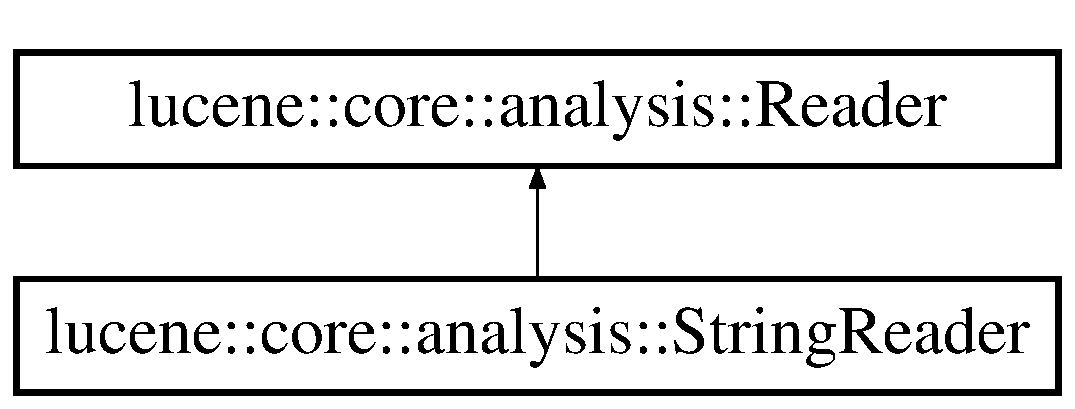
\includegraphics[height=2.000000cm]{classlucene_1_1core_1_1analysis_1_1StringReader}
\end{center}
\end{figure}
\subsection*{Public Member Functions}
\begin{DoxyCompactItemize}
\item 
\mbox{\hyperlink{classlucene_1_1core_1_1analysis_1_1StringReader_a58300c89dc23bee57f60fea22572d3da}{String\+Reader}} ()
\item 
\mbox{\hyperlink{classlucene_1_1core_1_1analysis_1_1StringReader_ac531f5f4b388f8a7cfd2ea0c2ef1a55c}{String\+Reader}} (\mbox{\hyperlink{ZlibCrc32_8h_a2c212835823e3c54a8ab6d95c652660e}{const}} \mbox{\hyperlink{classlucene_1_1core_1_1analysis_1_1StringReader}{String\+Reader}} \&other)
\item 
\mbox{\hyperlink{classlucene_1_1core_1_1analysis_1_1StringReader_accebdb26d787469d4f32f94c8c29257b}{String\+Reader}} (\mbox{\hyperlink{classlucene_1_1core_1_1analysis_1_1StringReader}{String\+Reader}} \&\&other)
\item 
\mbox{\hyperlink{classlucene_1_1core_1_1analysis_1_1StringReader_a72cb772b6be24d3f3c7055932a30a41d}{String\+Reader}} (\mbox{\hyperlink{ZlibCrc32_8h_a2c212835823e3c54a8ab6d95c652660e}{const}} std\+::string \&str)
\item 
\mbox{\hyperlink{classlucene_1_1core_1_1analysis_1_1StringReader_a2c3a2da6f1c5b1affbdee25ffcb235a6}{String\+Reader}} (\mbox{\hyperlink{ZlibCrc32_8h_a2c212835823e3c54a8ab6d95c652660e}{const}} char $\ast$cstr)
\item 
\mbox{\hyperlink{classlucene_1_1core_1_1analysis_1_1StringReader_a4c9a31c3c535283012a540e19077d1e5}{String\+Reader}} (\mbox{\hyperlink{ZlibCrc32_8h_a2c212835823e3c54a8ab6d95c652660e}{const}} char $\ast$cstr, \mbox{\hyperlink{ZlibCrc32_8h_a2c212835823e3c54a8ab6d95c652660e}{const}} unsigned len)
\item 
\mbox{\hyperlink{classlucene_1_1core_1_1analysis_1_1StringReader_a836d26003eca1d1def03daecf3487bfd}{String\+Reader}} (\mbox{\hyperlink{ZlibCrc32_8h_a2c212835823e3c54a8ab6d95c652660e}{const}} char $\ast$cstr, \mbox{\hyperlink{ZlibCrc32_8h_a2c212835823e3c54a8ab6d95c652660e}{const}} uint32\+\_\+t off, \mbox{\hyperlink{ZlibCrc32_8h_a2c212835823e3c54a8ab6d95c652660e}{const}} unsigned len)
\item 
\mbox{\hyperlink{classlucene_1_1core_1_1analysis_1_1StringReader_af30fe6285128fd4b1d2553017be84501}{String\+Reader}} (std\+::istringstream \&\mbox{\hyperlink{classlucene_1_1core_1_1analysis_1_1StringReader_ada023622e5d849d9fe8e9fcb838af328}{iss}})
\item 
\mbox{\hyperlink{classlucene_1_1core_1_1analysis_1_1StringReader_a47afb692b5f416dc38b25df9e46e79fc}{String\+Reader}} (std\+::istringstream \&\&\mbox{\hyperlink{classlucene_1_1core_1_1analysis_1_1StringReader_ada023622e5d849d9fe8e9fcb838af328}{iss}})
\item 
\mbox{\hyperlink{classlucene_1_1core_1_1analysis_1_1StringReader}{String\+Reader}} \& \mbox{\hyperlink{classlucene_1_1core_1_1analysis_1_1StringReader_ae79c2f5548c96bd451ebcb5a4f34ef0c}{operator=}} (\mbox{\hyperlink{ZlibCrc32_8h_a2c212835823e3c54a8ab6d95c652660e}{const}} \mbox{\hyperlink{classlucene_1_1core_1_1analysis_1_1StringReader}{String\+Reader}} \&other)
\item 
\mbox{\hyperlink{classlucene_1_1core_1_1analysis_1_1StringReader}{String\+Reader}} \& \mbox{\hyperlink{classlucene_1_1core_1_1analysis_1_1StringReader_a4ee9a9d9f36760e7d7a3495cb73efc70}{operator=}} (\mbox{\hyperlink{classlucene_1_1core_1_1analysis_1_1StringReader}{String\+Reader}} \&\&other)
\item 
\mbox{\hyperlink{classlucene_1_1core_1_1analysis_1_1StringReader}{String\+Reader}} \& \mbox{\hyperlink{classlucene_1_1core_1_1analysis_1_1StringReader_ae7440c5e8b7dd6f71a12986c55744e42}{operator=}} (std\+::istringstream \&new\+\_\+iss)
\item 
\mbox{\hyperlink{classlucene_1_1core_1_1analysis_1_1StringReader}{String\+Reader}} \& \mbox{\hyperlink{classlucene_1_1core_1_1analysis_1_1StringReader_a5278369c965094572c0b582fa87fe9ce}{operator=}} (std\+::istringstream \&\&new\+\_\+iss)
\item 
virtual \mbox{\hyperlink{classlucene_1_1core_1_1analysis_1_1StringReader_a9eb8a69da4acaa2c718b6dbc964552fb}{$\sim$\+String\+Reader}} ()
\item 
void \mbox{\hyperlink{classlucene_1_1core_1_1analysis_1_1StringReader_a2f707cdd271256c3cdf6e0004822612e}{Set\+Value}} (\mbox{\hyperlink{ZlibCrc32_8h_a2c212835823e3c54a8ab6d95c652660e}{const}} std\+::string \&value)
\item 
void \mbox{\hyperlink{classlucene_1_1core_1_1analysis_1_1StringReader_aeecb85481cb6e99493a0792e685f2fea}{Set\+Value}} (\mbox{\hyperlink{ZlibCrc32_8h_a2c212835823e3c54a8ab6d95c652660e}{const}} char $\ast$cstr)
\item 
void \mbox{\hyperlink{classlucene_1_1core_1_1analysis_1_1StringReader_ab28b0b0bfa46a28b55c0e4fe731cbaf8}{Set\+Value}} (\mbox{\hyperlink{ZlibCrc32_8h_a2c212835823e3c54a8ab6d95c652660e}{const}} char $\ast$cstr, \mbox{\hyperlink{ZlibCrc32_8h_a2c212835823e3c54a8ab6d95c652660e}{const}} uint32\+\_\+t len)
\item 
void \mbox{\hyperlink{classlucene_1_1core_1_1analysis_1_1StringReader_ac09c0dcf47934c6239845881b35c5aba}{Set\+Value}} (\mbox{\hyperlink{ZlibCrc32_8h_a2c212835823e3c54a8ab6d95c652660e}{const}} char $\ast$cstr, \mbox{\hyperlink{ZlibCrc32_8h_a2c212835823e3c54a8ab6d95c652660e}{const}} uint32\+\_\+t off, \mbox{\hyperlink{ZlibCrc32_8h_a2c212835823e3c54a8ab6d95c652660e}{const}} uint32\+\_\+t len)
\item 
int \mbox{\hyperlink{classlucene_1_1core_1_1analysis_1_1StringReader_ac9c1bb033ee4f5862e47e90c422d3381}{Read}} () override
\item 
void \mbox{\hyperlink{classlucene_1_1core_1_1analysis_1_1StringReader_a5bf198e593389f1255ec7a4f69f3187d}{Read\+Line}} (std\+::string \&line) override
\item 
int \mbox{\hyperlink{classlucene_1_1core_1_1analysis_1_1StringReader_ab048d6d6d759175eeda5321a480995c3}{Read}} (char $\ast$cstr, \mbox{\hyperlink{ZlibCrc32_8h_a2c212835823e3c54a8ab6d95c652660e}{const}} uint32\+\_\+t off, \mbox{\hyperlink{ZlibCrc32_8h_a2c212835823e3c54a8ab6d95c652660e}{const}} uint32\+\_\+t len) override
\item 
void \mbox{\hyperlink{classlucene_1_1core_1_1analysis_1_1StringReader_a745fa855b7308d2c08e289751590cdc7}{Skip}} (\mbox{\hyperlink{ZlibCrc32_8h_a2c212835823e3c54a8ab6d95c652660e}{const}} size\+\_\+t n) override
\item 
bool \mbox{\hyperlink{classlucene_1_1core_1_1analysis_1_1StringReader_a1b9e55036f01d10650fd4026f23da629}{Mark\+Supported}} () override
\item 
void \mbox{\hyperlink{classlucene_1_1core_1_1analysis_1_1StringReader_a0ba42881881e4790dae54bc1c01063f5}{Mark}} (\mbox{\hyperlink{ZlibCrc32_8h_a2c212835823e3c54a8ab6d95c652660e}{const}} uint32\+\_\+t read\+\_\+ahead\+\_\+limit) override
\item 
void \mbox{\hyperlink{classlucene_1_1core_1_1analysis_1_1StringReader_ab68ad2d8d2e375cd063c374c570fcffa}{Reset}} () override
\item 
void \mbox{\hyperlink{classlucene_1_1core_1_1analysis_1_1StringReader_ac2938d531e7842abb8423149982328e3}{Close}} () override
\item 
bool \mbox{\hyperlink{classlucene_1_1core_1_1analysis_1_1StringReader_a7697e462ff19e3e8fa135e38fa3e4999}{Eof}} () override
\end{DoxyCompactItemize}
\subsection*{Private Attributes}
\begin{DoxyCompactItemize}
\item 
std\+::istringstream \mbox{\hyperlink{classlucene_1_1core_1_1analysis_1_1StringReader_ada023622e5d849d9fe8e9fcb838af328}{iss}}
\item 
uint32\+\_\+t \mbox{\hyperlink{classlucene_1_1core_1_1analysis_1_1StringReader_a9a5cc9672f77bed7c252145fbde69176}{mark}}
\end{DoxyCompactItemize}


\subsection{Constructor \& Destructor Documentation}
\mbox{\Hypertarget{classlucene_1_1core_1_1analysis_1_1StringReader_a58300c89dc23bee57f60fea22572d3da}\label{classlucene_1_1core_1_1analysis_1_1StringReader_a58300c89dc23bee57f60fea22572d3da}} 
\index{lucene\+::core\+::analysis\+::\+String\+Reader@{lucene\+::core\+::analysis\+::\+String\+Reader}!String\+Reader@{String\+Reader}}
\index{String\+Reader@{String\+Reader}!lucene\+::core\+::analysis\+::\+String\+Reader@{lucene\+::core\+::analysis\+::\+String\+Reader}}
\subsubsection{\texorpdfstring{String\+Reader()}{StringReader()}\hspace{0.1cm}{\footnotesize\ttfamily [1/9]}}
{\footnotesize\ttfamily String\+Reader\+::\+String\+Reader (\begin{DoxyParamCaption}{ }\end{DoxyParamCaption})}

\mbox{\hyperlink{classlucene_1_1core_1_1analysis_1_1StringReader}{String\+Reader}} \mbox{\Hypertarget{classlucene_1_1core_1_1analysis_1_1StringReader_ac531f5f4b388f8a7cfd2ea0c2ef1a55c}\label{classlucene_1_1core_1_1analysis_1_1StringReader_ac531f5f4b388f8a7cfd2ea0c2ef1a55c}} 
\index{lucene\+::core\+::analysis\+::\+String\+Reader@{lucene\+::core\+::analysis\+::\+String\+Reader}!String\+Reader@{String\+Reader}}
\index{String\+Reader@{String\+Reader}!lucene\+::core\+::analysis\+::\+String\+Reader@{lucene\+::core\+::analysis\+::\+String\+Reader}}
\subsubsection{\texorpdfstring{String\+Reader()}{StringReader()}\hspace{0.1cm}{\footnotesize\ttfamily [2/9]}}
{\footnotesize\ttfamily String\+Reader\+::\+String\+Reader (\begin{DoxyParamCaption}\item[{\mbox{\hyperlink{ZlibCrc32_8h_a2c212835823e3c54a8ab6d95c652660e}{const}} \mbox{\hyperlink{classlucene_1_1core_1_1analysis_1_1StringReader}{String\+Reader}} \&}]{other }\end{DoxyParamCaption})}

\mbox{\Hypertarget{classlucene_1_1core_1_1analysis_1_1StringReader_accebdb26d787469d4f32f94c8c29257b}\label{classlucene_1_1core_1_1analysis_1_1StringReader_accebdb26d787469d4f32f94c8c29257b}} 
\index{lucene\+::core\+::analysis\+::\+String\+Reader@{lucene\+::core\+::analysis\+::\+String\+Reader}!String\+Reader@{String\+Reader}}
\index{String\+Reader@{String\+Reader}!lucene\+::core\+::analysis\+::\+String\+Reader@{lucene\+::core\+::analysis\+::\+String\+Reader}}
\subsubsection{\texorpdfstring{String\+Reader()}{StringReader()}\hspace{0.1cm}{\footnotesize\ttfamily [3/9]}}
{\footnotesize\ttfamily String\+Reader\+::\+String\+Reader (\begin{DoxyParamCaption}\item[{\mbox{\hyperlink{classlucene_1_1core_1_1analysis_1_1StringReader}{String\+Reader}} \&\&}]{other }\end{DoxyParamCaption})}

\mbox{\Hypertarget{classlucene_1_1core_1_1analysis_1_1StringReader_a72cb772b6be24d3f3c7055932a30a41d}\label{classlucene_1_1core_1_1analysis_1_1StringReader_a72cb772b6be24d3f3c7055932a30a41d}} 
\index{lucene\+::core\+::analysis\+::\+String\+Reader@{lucene\+::core\+::analysis\+::\+String\+Reader}!String\+Reader@{String\+Reader}}
\index{String\+Reader@{String\+Reader}!lucene\+::core\+::analysis\+::\+String\+Reader@{lucene\+::core\+::analysis\+::\+String\+Reader}}
\subsubsection{\texorpdfstring{String\+Reader()}{StringReader()}\hspace{0.1cm}{\footnotesize\ttfamily [4/9]}}
{\footnotesize\ttfamily String\+Reader\+::\+String\+Reader (\begin{DoxyParamCaption}\item[{\mbox{\hyperlink{ZlibCrc32_8h_a2c212835823e3c54a8ab6d95c652660e}{const}} std\+::string \&}]{str }\end{DoxyParamCaption})\hspace{0.3cm}{\ttfamily [explicit]}}

\mbox{\Hypertarget{classlucene_1_1core_1_1analysis_1_1StringReader_a2c3a2da6f1c5b1affbdee25ffcb235a6}\label{classlucene_1_1core_1_1analysis_1_1StringReader_a2c3a2da6f1c5b1affbdee25ffcb235a6}} 
\index{lucene\+::core\+::analysis\+::\+String\+Reader@{lucene\+::core\+::analysis\+::\+String\+Reader}!String\+Reader@{String\+Reader}}
\index{String\+Reader@{String\+Reader}!lucene\+::core\+::analysis\+::\+String\+Reader@{lucene\+::core\+::analysis\+::\+String\+Reader}}
\subsubsection{\texorpdfstring{String\+Reader()}{StringReader()}\hspace{0.1cm}{\footnotesize\ttfamily [5/9]}}
{\footnotesize\ttfamily String\+Reader\+::\+String\+Reader (\begin{DoxyParamCaption}\item[{\mbox{\hyperlink{ZlibCrc32_8h_a2c212835823e3c54a8ab6d95c652660e}{const}} char $\ast$}]{cstr }\end{DoxyParamCaption})\hspace{0.3cm}{\ttfamily [explicit]}}

\mbox{\Hypertarget{classlucene_1_1core_1_1analysis_1_1StringReader_a4c9a31c3c535283012a540e19077d1e5}\label{classlucene_1_1core_1_1analysis_1_1StringReader_a4c9a31c3c535283012a540e19077d1e5}} 
\index{lucene\+::core\+::analysis\+::\+String\+Reader@{lucene\+::core\+::analysis\+::\+String\+Reader}!String\+Reader@{String\+Reader}}
\index{String\+Reader@{String\+Reader}!lucene\+::core\+::analysis\+::\+String\+Reader@{lucene\+::core\+::analysis\+::\+String\+Reader}}
\subsubsection{\texorpdfstring{String\+Reader()}{StringReader()}\hspace{0.1cm}{\footnotesize\ttfamily [6/9]}}
{\footnotesize\ttfamily String\+Reader\+::\+String\+Reader (\begin{DoxyParamCaption}\item[{\mbox{\hyperlink{ZlibCrc32_8h_a2c212835823e3c54a8ab6d95c652660e}{const}} char $\ast$}]{cstr,  }\item[{\mbox{\hyperlink{ZlibCrc32_8h_a2c212835823e3c54a8ab6d95c652660e}{const}} unsigned}]{len }\end{DoxyParamCaption})}

\mbox{\Hypertarget{classlucene_1_1core_1_1analysis_1_1StringReader_a836d26003eca1d1def03daecf3487bfd}\label{classlucene_1_1core_1_1analysis_1_1StringReader_a836d26003eca1d1def03daecf3487bfd}} 
\index{lucene\+::core\+::analysis\+::\+String\+Reader@{lucene\+::core\+::analysis\+::\+String\+Reader}!String\+Reader@{String\+Reader}}
\index{String\+Reader@{String\+Reader}!lucene\+::core\+::analysis\+::\+String\+Reader@{lucene\+::core\+::analysis\+::\+String\+Reader}}
\subsubsection{\texorpdfstring{String\+Reader()}{StringReader()}\hspace{0.1cm}{\footnotesize\ttfamily [7/9]}}
{\footnotesize\ttfamily String\+Reader\+::\+String\+Reader (\begin{DoxyParamCaption}\item[{\mbox{\hyperlink{ZlibCrc32_8h_a2c212835823e3c54a8ab6d95c652660e}{const}} char $\ast$}]{cstr,  }\item[{\mbox{\hyperlink{ZlibCrc32_8h_a2c212835823e3c54a8ab6d95c652660e}{const}} uint32\+\_\+t}]{off,  }\item[{\mbox{\hyperlink{ZlibCrc32_8h_a2c212835823e3c54a8ab6d95c652660e}{const}} unsigned}]{len }\end{DoxyParamCaption})}

\mbox{\Hypertarget{classlucene_1_1core_1_1analysis_1_1StringReader_af30fe6285128fd4b1d2553017be84501}\label{classlucene_1_1core_1_1analysis_1_1StringReader_af30fe6285128fd4b1d2553017be84501}} 
\index{lucene\+::core\+::analysis\+::\+String\+Reader@{lucene\+::core\+::analysis\+::\+String\+Reader}!String\+Reader@{String\+Reader}}
\index{String\+Reader@{String\+Reader}!lucene\+::core\+::analysis\+::\+String\+Reader@{lucene\+::core\+::analysis\+::\+String\+Reader}}
\subsubsection{\texorpdfstring{String\+Reader()}{StringReader()}\hspace{0.1cm}{\footnotesize\ttfamily [8/9]}}
{\footnotesize\ttfamily String\+Reader\+::\+String\+Reader (\begin{DoxyParamCaption}\item[{std\+::istringstream \&}]{iss }\end{DoxyParamCaption})\hspace{0.3cm}{\ttfamily [explicit]}}

\mbox{\Hypertarget{classlucene_1_1core_1_1analysis_1_1StringReader_a47afb692b5f416dc38b25df9e46e79fc}\label{classlucene_1_1core_1_1analysis_1_1StringReader_a47afb692b5f416dc38b25df9e46e79fc}} 
\index{lucene\+::core\+::analysis\+::\+String\+Reader@{lucene\+::core\+::analysis\+::\+String\+Reader}!String\+Reader@{String\+Reader}}
\index{String\+Reader@{String\+Reader}!lucene\+::core\+::analysis\+::\+String\+Reader@{lucene\+::core\+::analysis\+::\+String\+Reader}}
\subsubsection{\texorpdfstring{String\+Reader()}{StringReader()}\hspace{0.1cm}{\footnotesize\ttfamily [9/9]}}
{\footnotesize\ttfamily String\+Reader\+::\+String\+Reader (\begin{DoxyParamCaption}\item[{std\+::istringstream \&\&}]{iss }\end{DoxyParamCaption})\hspace{0.3cm}{\ttfamily [explicit]}}

\mbox{\Hypertarget{classlucene_1_1core_1_1analysis_1_1StringReader_a9eb8a69da4acaa2c718b6dbc964552fb}\label{classlucene_1_1core_1_1analysis_1_1StringReader_a9eb8a69da4acaa2c718b6dbc964552fb}} 
\index{lucene\+::core\+::analysis\+::\+String\+Reader@{lucene\+::core\+::analysis\+::\+String\+Reader}!````~String\+Reader@{$\sim$\+String\+Reader}}
\index{````~String\+Reader@{$\sim$\+String\+Reader}!lucene\+::core\+::analysis\+::\+String\+Reader@{lucene\+::core\+::analysis\+::\+String\+Reader}}
\subsubsection{\texorpdfstring{$\sim$\+String\+Reader()}{~StringReader()}}
{\footnotesize\ttfamily String\+Reader\+::$\sim$\+String\+Reader (\begin{DoxyParamCaption}{ }\end{DoxyParamCaption})\hspace{0.3cm}{\ttfamily [virtual]}}



\subsection{Member Function Documentation}
\mbox{\Hypertarget{classlucene_1_1core_1_1analysis_1_1StringReader_ac2938d531e7842abb8423149982328e3}\label{classlucene_1_1core_1_1analysis_1_1StringReader_ac2938d531e7842abb8423149982328e3}} 
\index{lucene\+::core\+::analysis\+::\+String\+Reader@{lucene\+::core\+::analysis\+::\+String\+Reader}!Close@{Close}}
\index{Close@{Close}!lucene\+::core\+::analysis\+::\+String\+Reader@{lucene\+::core\+::analysis\+::\+String\+Reader}}
\subsubsection{\texorpdfstring{Close()}{Close()}}
{\footnotesize\ttfamily void String\+Reader\+::\+Close (\begin{DoxyParamCaption}{ }\end{DoxyParamCaption})\hspace{0.3cm}{\ttfamily [override]}, {\ttfamily [virtual]}}



Implements \mbox{\hyperlink{classlucene_1_1core_1_1analysis_1_1Reader_a4be7e96dccdd3e276e3450e3ad7a70f4}{lucene\+::core\+::analysis\+::\+Reader}}.

\mbox{\Hypertarget{classlucene_1_1core_1_1analysis_1_1StringReader_a7697e462ff19e3e8fa135e38fa3e4999}\label{classlucene_1_1core_1_1analysis_1_1StringReader_a7697e462ff19e3e8fa135e38fa3e4999}} 
\index{lucene\+::core\+::analysis\+::\+String\+Reader@{lucene\+::core\+::analysis\+::\+String\+Reader}!Eof@{Eof}}
\index{Eof@{Eof}!lucene\+::core\+::analysis\+::\+String\+Reader@{lucene\+::core\+::analysis\+::\+String\+Reader}}
\subsubsection{\texorpdfstring{Eof()}{Eof()}}
{\footnotesize\ttfamily bool String\+Reader\+::\+Eof (\begin{DoxyParamCaption}{ }\end{DoxyParamCaption})\hspace{0.3cm}{\ttfamily [override]}, {\ttfamily [virtual]}}



Implements \mbox{\hyperlink{classlucene_1_1core_1_1analysis_1_1Reader_af7a24f3904f9c40e9c5c204b3434f1f7}{lucene\+::core\+::analysis\+::\+Reader}}.

\mbox{\Hypertarget{classlucene_1_1core_1_1analysis_1_1StringReader_a0ba42881881e4790dae54bc1c01063f5}\label{classlucene_1_1core_1_1analysis_1_1StringReader_a0ba42881881e4790dae54bc1c01063f5}} 
\index{lucene\+::core\+::analysis\+::\+String\+Reader@{lucene\+::core\+::analysis\+::\+String\+Reader}!Mark@{Mark}}
\index{Mark@{Mark}!lucene\+::core\+::analysis\+::\+String\+Reader@{lucene\+::core\+::analysis\+::\+String\+Reader}}
\subsubsection{\texorpdfstring{Mark()}{Mark()}}
{\footnotesize\ttfamily void String\+Reader\+::\+Mark (\begin{DoxyParamCaption}\item[{\mbox{\hyperlink{ZlibCrc32_8h_a2c212835823e3c54a8ab6d95c652660e}{const}} uint32\+\_\+t}]{read\+\_\+ahead\+\_\+limit }\end{DoxyParamCaption})\hspace{0.3cm}{\ttfamily [override]}, {\ttfamily [virtual]}}



Implements \mbox{\hyperlink{classlucene_1_1core_1_1analysis_1_1Reader_a0b60b07a3f65098a50f10f6618097527}{lucene\+::core\+::analysis\+::\+Reader}}.

\mbox{\Hypertarget{classlucene_1_1core_1_1analysis_1_1StringReader_a1b9e55036f01d10650fd4026f23da629}\label{classlucene_1_1core_1_1analysis_1_1StringReader_a1b9e55036f01d10650fd4026f23da629}} 
\index{lucene\+::core\+::analysis\+::\+String\+Reader@{lucene\+::core\+::analysis\+::\+String\+Reader}!Mark\+Supported@{Mark\+Supported}}
\index{Mark\+Supported@{Mark\+Supported}!lucene\+::core\+::analysis\+::\+String\+Reader@{lucene\+::core\+::analysis\+::\+String\+Reader}}
\subsubsection{\texorpdfstring{Mark\+Supported()}{MarkSupported()}}
{\footnotesize\ttfamily bool String\+Reader\+::\+Mark\+Supported (\begin{DoxyParamCaption}{ }\end{DoxyParamCaption})\hspace{0.3cm}{\ttfamily [override]}, {\ttfamily [virtual]}}



Implements \mbox{\hyperlink{classlucene_1_1core_1_1analysis_1_1Reader_a230fae02ca4a63de33fdaad6f9aafd96}{lucene\+::core\+::analysis\+::\+Reader}}.

\mbox{\Hypertarget{classlucene_1_1core_1_1analysis_1_1StringReader_ae79c2f5548c96bd451ebcb5a4f34ef0c}\label{classlucene_1_1core_1_1analysis_1_1StringReader_ae79c2f5548c96bd451ebcb5a4f34ef0c}} 
\index{lucene\+::core\+::analysis\+::\+String\+Reader@{lucene\+::core\+::analysis\+::\+String\+Reader}!operator=@{operator=}}
\index{operator=@{operator=}!lucene\+::core\+::analysis\+::\+String\+Reader@{lucene\+::core\+::analysis\+::\+String\+Reader}}
\subsubsection{\texorpdfstring{operator=()}{operator=()}\hspace{0.1cm}{\footnotesize\ttfamily [1/4]}}
{\footnotesize\ttfamily \mbox{\hyperlink{classlucene_1_1core_1_1analysis_1_1StringReader}{String\+Reader}} \& String\+Reader\+::operator= (\begin{DoxyParamCaption}\item[{\mbox{\hyperlink{ZlibCrc32_8h_a2c212835823e3c54a8ab6d95c652660e}{const}} \mbox{\hyperlink{classlucene_1_1core_1_1analysis_1_1StringReader}{String\+Reader}} \&}]{other }\end{DoxyParamCaption})}

\mbox{\Hypertarget{classlucene_1_1core_1_1analysis_1_1StringReader_a4ee9a9d9f36760e7d7a3495cb73efc70}\label{classlucene_1_1core_1_1analysis_1_1StringReader_a4ee9a9d9f36760e7d7a3495cb73efc70}} 
\index{lucene\+::core\+::analysis\+::\+String\+Reader@{lucene\+::core\+::analysis\+::\+String\+Reader}!operator=@{operator=}}
\index{operator=@{operator=}!lucene\+::core\+::analysis\+::\+String\+Reader@{lucene\+::core\+::analysis\+::\+String\+Reader}}
\subsubsection{\texorpdfstring{operator=()}{operator=()}\hspace{0.1cm}{\footnotesize\ttfamily [2/4]}}
{\footnotesize\ttfamily \mbox{\hyperlink{classlucene_1_1core_1_1analysis_1_1StringReader}{String\+Reader}} \& String\+Reader\+::operator= (\begin{DoxyParamCaption}\item[{\mbox{\hyperlink{classlucene_1_1core_1_1analysis_1_1StringReader}{String\+Reader}} \&\&}]{other }\end{DoxyParamCaption})}

\mbox{\Hypertarget{classlucene_1_1core_1_1analysis_1_1StringReader_ae7440c5e8b7dd6f71a12986c55744e42}\label{classlucene_1_1core_1_1analysis_1_1StringReader_ae7440c5e8b7dd6f71a12986c55744e42}} 
\index{lucene\+::core\+::analysis\+::\+String\+Reader@{lucene\+::core\+::analysis\+::\+String\+Reader}!operator=@{operator=}}
\index{operator=@{operator=}!lucene\+::core\+::analysis\+::\+String\+Reader@{lucene\+::core\+::analysis\+::\+String\+Reader}}
\subsubsection{\texorpdfstring{operator=()}{operator=()}\hspace{0.1cm}{\footnotesize\ttfamily [3/4]}}
{\footnotesize\ttfamily \mbox{\hyperlink{classlucene_1_1core_1_1analysis_1_1StringReader}{String\+Reader}} \& String\+Reader\+::operator= (\begin{DoxyParamCaption}\item[{std\+::istringstream \&}]{new\+\_\+iss }\end{DoxyParamCaption})}

\mbox{\Hypertarget{classlucene_1_1core_1_1analysis_1_1StringReader_a5278369c965094572c0b582fa87fe9ce}\label{classlucene_1_1core_1_1analysis_1_1StringReader_a5278369c965094572c0b582fa87fe9ce}} 
\index{lucene\+::core\+::analysis\+::\+String\+Reader@{lucene\+::core\+::analysis\+::\+String\+Reader}!operator=@{operator=}}
\index{operator=@{operator=}!lucene\+::core\+::analysis\+::\+String\+Reader@{lucene\+::core\+::analysis\+::\+String\+Reader}}
\subsubsection{\texorpdfstring{operator=()}{operator=()}\hspace{0.1cm}{\footnotesize\ttfamily [4/4]}}
{\footnotesize\ttfamily \mbox{\hyperlink{classlucene_1_1core_1_1analysis_1_1StringReader}{String\+Reader}} \& String\+Reader\+::operator= (\begin{DoxyParamCaption}\item[{std\+::istringstream \&\&}]{new\+\_\+iss }\end{DoxyParamCaption})}

\mbox{\Hypertarget{classlucene_1_1core_1_1analysis_1_1StringReader_ac9c1bb033ee4f5862e47e90c422d3381}\label{classlucene_1_1core_1_1analysis_1_1StringReader_ac9c1bb033ee4f5862e47e90c422d3381}} 
\index{lucene\+::core\+::analysis\+::\+String\+Reader@{lucene\+::core\+::analysis\+::\+String\+Reader}!Read@{Read}}
\index{Read@{Read}!lucene\+::core\+::analysis\+::\+String\+Reader@{lucene\+::core\+::analysis\+::\+String\+Reader}}
\subsubsection{\texorpdfstring{Read()}{Read()}\hspace{0.1cm}{\footnotesize\ttfamily [1/2]}}
{\footnotesize\ttfamily int String\+Reader\+::\+Read (\begin{DoxyParamCaption}{ }\end{DoxyParamCaption})\hspace{0.3cm}{\ttfamily [override]}, {\ttfamily [virtual]}}



Implements \mbox{\hyperlink{classlucene_1_1core_1_1analysis_1_1Reader_ae8e04911b6a4c06bb026ca6e74071cb2}{lucene\+::core\+::analysis\+::\+Reader}}.

\mbox{\Hypertarget{classlucene_1_1core_1_1analysis_1_1StringReader_ab048d6d6d759175eeda5321a480995c3}\label{classlucene_1_1core_1_1analysis_1_1StringReader_ab048d6d6d759175eeda5321a480995c3}} 
\index{lucene\+::core\+::analysis\+::\+String\+Reader@{lucene\+::core\+::analysis\+::\+String\+Reader}!Read@{Read}}
\index{Read@{Read}!lucene\+::core\+::analysis\+::\+String\+Reader@{lucene\+::core\+::analysis\+::\+String\+Reader}}
\subsubsection{\texorpdfstring{Read()}{Read()}\hspace{0.1cm}{\footnotesize\ttfamily [2/2]}}
{\footnotesize\ttfamily int32\+\_\+t String\+Reader\+::\+Read (\begin{DoxyParamCaption}\item[{char $\ast$}]{cstr,  }\item[{\mbox{\hyperlink{ZlibCrc32_8h_a2c212835823e3c54a8ab6d95c652660e}{const}} uint32\+\_\+t}]{off,  }\item[{\mbox{\hyperlink{ZlibCrc32_8h_a2c212835823e3c54a8ab6d95c652660e}{const}} uint32\+\_\+t}]{len }\end{DoxyParamCaption})\hspace{0.3cm}{\ttfamily [override]}, {\ttfamily [virtual]}}



Implements \mbox{\hyperlink{classlucene_1_1core_1_1analysis_1_1Reader_a986e25a49a947dc113a22c6de033ebe9}{lucene\+::core\+::analysis\+::\+Reader}}.

\mbox{\Hypertarget{classlucene_1_1core_1_1analysis_1_1StringReader_a5bf198e593389f1255ec7a4f69f3187d}\label{classlucene_1_1core_1_1analysis_1_1StringReader_a5bf198e593389f1255ec7a4f69f3187d}} 
\index{lucene\+::core\+::analysis\+::\+String\+Reader@{lucene\+::core\+::analysis\+::\+String\+Reader}!Read\+Line@{Read\+Line}}
\index{Read\+Line@{Read\+Line}!lucene\+::core\+::analysis\+::\+String\+Reader@{lucene\+::core\+::analysis\+::\+String\+Reader}}
\subsubsection{\texorpdfstring{Read\+Line()}{ReadLine()}}
{\footnotesize\ttfamily void String\+Reader\+::\+Read\+Line (\begin{DoxyParamCaption}\item[{std\+::string \&}]{line }\end{DoxyParamCaption})\hspace{0.3cm}{\ttfamily [override]}, {\ttfamily [virtual]}}



Implements \mbox{\hyperlink{classlucene_1_1core_1_1analysis_1_1Reader_a475ba046fd74e43a1cce4c4702c791c2}{lucene\+::core\+::analysis\+::\+Reader}}.

\mbox{\Hypertarget{classlucene_1_1core_1_1analysis_1_1StringReader_ab68ad2d8d2e375cd063c374c570fcffa}\label{classlucene_1_1core_1_1analysis_1_1StringReader_ab68ad2d8d2e375cd063c374c570fcffa}} 
\index{lucene\+::core\+::analysis\+::\+String\+Reader@{lucene\+::core\+::analysis\+::\+String\+Reader}!Reset@{Reset}}
\index{Reset@{Reset}!lucene\+::core\+::analysis\+::\+String\+Reader@{lucene\+::core\+::analysis\+::\+String\+Reader}}
\subsubsection{\texorpdfstring{Reset()}{Reset()}}
{\footnotesize\ttfamily void String\+Reader\+::\+Reset (\begin{DoxyParamCaption}{ }\end{DoxyParamCaption})\hspace{0.3cm}{\ttfamily [override]}, {\ttfamily [virtual]}}



Implements \mbox{\hyperlink{classlucene_1_1core_1_1analysis_1_1Reader_a5299f5469ce4ea9812ec79a59667945a}{lucene\+::core\+::analysis\+::\+Reader}}.

\mbox{\Hypertarget{classlucene_1_1core_1_1analysis_1_1StringReader_a2f707cdd271256c3cdf6e0004822612e}\label{classlucene_1_1core_1_1analysis_1_1StringReader_a2f707cdd271256c3cdf6e0004822612e}} 
\index{lucene\+::core\+::analysis\+::\+String\+Reader@{lucene\+::core\+::analysis\+::\+String\+Reader}!Set\+Value@{Set\+Value}}
\index{Set\+Value@{Set\+Value}!lucene\+::core\+::analysis\+::\+String\+Reader@{lucene\+::core\+::analysis\+::\+String\+Reader}}
\subsubsection{\texorpdfstring{Set\+Value()}{SetValue()}\hspace{0.1cm}{\footnotesize\ttfamily [1/4]}}
{\footnotesize\ttfamily void String\+Reader\+::\+Set\+Value (\begin{DoxyParamCaption}\item[{\mbox{\hyperlink{ZlibCrc32_8h_a2c212835823e3c54a8ab6d95c652660e}{const}} std\+::string \&}]{value }\end{DoxyParamCaption})}

\mbox{\Hypertarget{classlucene_1_1core_1_1analysis_1_1StringReader_aeecb85481cb6e99493a0792e685f2fea}\label{classlucene_1_1core_1_1analysis_1_1StringReader_aeecb85481cb6e99493a0792e685f2fea}} 
\index{lucene\+::core\+::analysis\+::\+String\+Reader@{lucene\+::core\+::analysis\+::\+String\+Reader}!Set\+Value@{Set\+Value}}
\index{Set\+Value@{Set\+Value}!lucene\+::core\+::analysis\+::\+String\+Reader@{lucene\+::core\+::analysis\+::\+String\+Reader}}
\subsubsection{\texorpdfstring{Set\+Value()}{SetValue()}\hspace{0.1cm}{\footnotesize\ttfamily [2/4]}}
{\footnotesize\ttfamily void String\+Reader\+::\+Set\+Value (\begin{DoxyParamCaption}\item[{\mbox{\hyperlink{ZlibCrc32_8h_a2c212835823e3c54a8ab6d95c652660e}{const}} char $\ast$}]{cstr }\end{DoxyParamCaption})}

\mbox{\Hypertarget{classlucene_1_1core_1_1analysis_1_1StringReader_ab28b0b0bfa46a28b55c0e4fe731cbaf8}\label{classlucene_1_1core_1_1analysis_1_1StringReader_ab28b0b0bfa46a28b55c0e4fe731cbaf8}} 
\index{lucene\+::core\+::analysis\+::\+String\+Reader@{lucene\+::core\+::analysis\+::\+String\+Reader}!Set\+Value@{Set\+Value}}
\index{Set\+Value@{Set\+Value}!lucene\+::core\+::analysis\+::\+String\+Reader@{lucene\+::core\+::analysis\+::\+String\+Reader}}
\subsubsection{\texorpdfstring{Set\+Value()}{SetValue()}\hspace{0.1cm}{\footnotesize\ttfamily [3/4]}}
{\footnotesize\ttfamily void String\+Reader\+::\+Set\+Value (\begin{DoxyParamCaption}\item[{\mbox{\hyperlink{ZlibCrc32_8h_a2c212835823e3c54a8ab6d95c652660e}{const}} char $\ast$}]{cstr,  }\item[{\mbox{\hyperlink{ZlibCrc32_8h_a2c212835823e3c54a8ab6d95c652660e}{const}} uint32\+\_\+t}]{len }\end{DoxyParamCaption})}

\mbox{\Hypertarget{classlucene_1_1core_1_1analysis_1_1StringReader_ac09c0dcf47934c6239845881b35c5aba}\label{classlucene_1_1core_1_1analysis_1_1StringReader_ac09c0dcf47934c6239845881b35c5aba}} 
\index{lucene\+::core\+::analysis\+::\+String\+Reader@{lucene\+::core\+::analysis\+::\+String\+Reader}!Set\+Value@{Set\+Value}}
\index{Set\+Value@{Set\+Value}!lucene\+::core\+::analysis\+::\+String\+Reader@{lucene\+::core\+::analysis\+::\+String\+Reader}}
\subsubsection{\texorpdfstring{Set\+Value()}{SetValue()}\hspace{0.1cm}{\footnotesize\ttfamily [4/4]}}
{\footnotesize\ttfamily void String\+Reader\+::\+Set\+Value (\begin{DoxyParamCaption}\item[{\mbox{\hyperlink{ZlibCrc32_8h_a2c212835823e3c54a8ab6d95c652660e}{const}} char $\ast$}]{cstr,  }\item[{\mbox{\hyperlink{ZlibCrc32_8h_a2c212835823e3c54a8ab6d95c652660e}{const}} uint32\+\_\+t}]{off,  }\item[{\mbox{\hyperlink{ZlibCrc32_8h_a2c212835823e3c54a8ab6d95c652660e}{const}} uint32\+\_\+t}]{len }\end{DoxyParamCaption})}

\mbox{\Hypertarget{classlucene_1_1core_1_1analysis_1_1StringReader_a745fa855b7308d2c08e289751590cdc7}\label{classlucene_1_1core_1_1analysis_1_1StringReader_a745fa855b7308d2c08e289751590cdc7}} 
\index{lucene\+::core\+::analysis\+::\+String\+Reader@{lucene\+::core\+::analysis\+::\+String\+Reader}!Skip@{Skip}}
\index{Skip@{Skip}!lucene\+::core\+::analysis\+::\+String\+Reader@{lucene\+::core\+::analysis\+::\+String\+Reader}}
\subsubsection{\texorpdfstring{Skip()}{Skip()}}
{\footnotesize\ttfamily void String\+Reader\+::\+Skip (\begin{DoxyParamCaption}\item[{\mbox{\hyperlink{ZlibCrc32_8h_a2c212835823e3c54a8ab6d95c652660e}{const}} size\+\_\+t}]{n }\end{DoxyParamCaption})\hspace{0.3cm}{\ttfamily [override]}}



\subsection{Member Data Documentation}
\mbox{\Hypertarget{classlucene_1_1core_1_1analysis_1_1StringReader_ada023622e5d849d9fe8e9fcb838af328}\label{classlucene_1_1core_1_1analysis_1_1StringReader_ada023622e5d849d9fe8e9fcb838af328}} 
\index{lucene\+::core\+::analysis\+::\+String\+Reader@{lucene\+::core\+::analysis\+::\+String\+Reader}!iss@{iss}}
\index{iss@{iss}!lucene\+::core\+::analysis\+::\+String\+Reader@{lucene\+::core\+::analysis\+::\+String\+Reader}}
\subsubsection{\texorpdfstring{iss}{iss}}
{\footnotesize\ttfamily std\+::istringstream lucene\+::core\+::analysis\+::\+String\+Reader\+::iss\hspace{0.3cm}{\ttfamily [private]}}

\mbox{\Hypertarget{classlucene_1_1core_1_1analysis_1_1StringReader_a9a5cc9672f77bed7c252145fbde69176}\label{classlucene_1_1core_1_1analysis_1_1StringReader_a9a5cc9672f77bed7c252145fbde69176}} 
\index{lucene\+::core\+::analysis\+::\+String\+Reader@{lucene\+::core\+::analysis\+::\+String\+Reader}!mark@{mark}}
\index{mark@{mark}!lucene\+::core\+::analysis\+::\+String\+Reader@{lucene\+::core\+::analysis\+::\+String\+Reader}}
\subsubsection{\texorpdfstring{mark}{mark}}
{\footnotesize\ttfamily uint32\+\_\+t lucene\+::core\+::analysis\+::\+String\+Reader\+::mark\hspace{0.3cm}{\ttfamily [private]}}



The documentation for this class was generated from the following files\+:\begin{DoxyCompactItemize}
\item 
Analysis/\mbox{\hyperlink{Reader_8h}{Reader.\+h}}\item 
Analysis/\mbox{\hyperlink{Reader_8cpp}{Reader.\+cpp}}\end{DoxyCompactItemize}

\hypertarget{classlucene_1_1core_1_1analysis_1_1StringTokenStream}{}\section{lucene\+:\+:core\+:\+:analysis\+:\+:String\+Token\+Stream Class Reference}
\label{classlucene_1_1core_1_1analysis_1_1StringTokenStream}\index{lucene\+::core\+::analysis\+::\+String\+Token\+Stream@{lucene\+::core\+::analysis\+::\+String\+Token\+Stream}}


{\ttfamily \#include $<$Analyzer.\+h$>$}

Inheritance diagram for lucene\+:\+:core\+:\+:analysis\+:\+:String\+Token\+Stream\+:\begin{figure}[H]
\begin{center}
\leavevmode
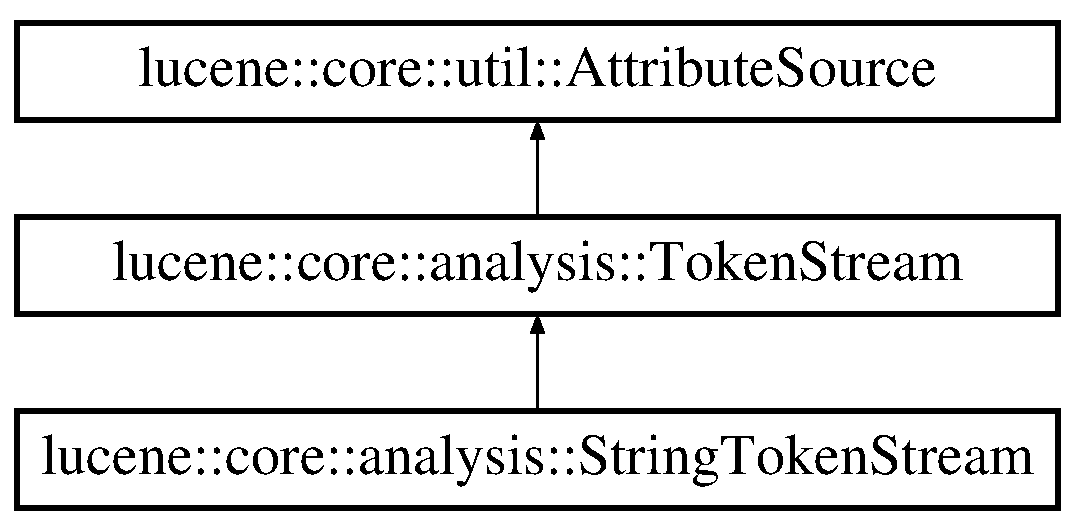
\includegraphics[height=3.000000cm]{classlucene_1_1core_1_1analysis_1_1StringTokenStream}
\end{center}
\end{figure}
\subsection*{Public Member Functions}
\begin{DoxyCompactItemize}
\item 
\mbox{\hyperlink{classlucene_1_1core_1_1analysis_1_1StringTokenStream_a413ff02bcf7a9f2d617f9e25021f9a44}{String\+Token\+Stream}} (\mbox{\hyperlink{classlucene_1_1core_1_1util_1_1AttributeFactory}{lucene\+::core\+::util\+::\+Attribute\+Factory}} \&input, std\+::string \&\mbox{\hyperlink{classlucene_1_1core_1_1analysis_1_1StringTokenStream_a6fb3e249a092b3cd9b008449d256b6a8}{value}}, size\+\_\+t \mbox{\hyperlink{classlucene_1_1core_1_1analysis_1_1StringTokenStream_ad16af1e525efb086aac50b843f80b418}{length}})
\item 
void \mbox{\hyperlink{classlucene_1_1core_1_1analysis_1_1StringTokenStream_ab578e75921eb1757b4a8887cf29fe94d}{Reset}} () override
\item 
bool \mbox{\hyperlink{classlucene_1_1core_1_1analysis_1_1StringTokenStream_a059da09c86bcf50a286803cad1b99d10}{Increment\+Token}} () override
\item 
void \mbox{\hyperlink{classlucene_1_1core_1_1analysis_1_1StringTokenStream_aabf9a873c934aff5c359417488f33849}{End}} () override
\end{DoxyCompactItemize}
\subsection*{Private Attributes}
\begin{DoxyCompactItemize}
\item 
std\+::string \& \mbox{\hyperlink{classlucene_1_1core_1_1analysis_1_1StringTokenStream_a6fb3e249a092b3cd9b008449d256b6a8}{value}}
\item 
size\+\_\+t \mbox{\hyperlink{classlucene_1_1core_1_1analysis_1_1StringTokenStream_ad16af1e525efb086aac50b843f80b418}{length}}
\item 
bool \mbox{\hyperlink{classlucene_1_1core_1_1analysis_1_1StringTokenStream_a26d177c979b40cc9ea6928567906cc87}{used}}
\item 
std\+::shared\+\_\+ptr$<$ \mbox{\hyperlink{classlucene_1_1core_1_1analysis_1_1tokenattributes_1_1CharTermAttribute}{tokenattributes\+::\+Char\+Term\+Attribute}} $>$ \mbox{\hyperlink{classlucene_1_1core_1_1analysis_1_1StringTokenStream_a4fcb486b031bc4d32047e09643da3099}{term\+\_\+attribute}}
\item 
std\+::shared\+\_\+ptr$<$ \mbox{\hyperlink{classlucene_1_1core_1_1analysis_1_1tokenattributes_1_1OffsetAttribute}{tokenattributes\+::\+Offset\+Attribute}} $>$ \mbox{\hyperlink{classlucene_1_1core_1_1analysis_1_1StringTokenStream_a52378286cf3479adf7932ff4555e2b0f}{offset\+\_\+attribute}}
\end{DoxyCompactItemize}
\subsection*{Additional Inherited Members}


\subsection{Constructor \& Destructor Documentation}
\mbox{\Hypertarget{classlucene_1_1core_1_1analysis_1_1StringTokenStream_a413ff02bcf7a9f2d617f9e25021f9a44}\label{classlucene_1_1core_1_1analysis_1_1StringTokenStream_a413ff02bcf7a9f2d617f9e25021f9a44}} 
\index{lucene\+::core\+::analysis\+::\+String\+Token\+Stream@{lucene\+::core\+::analysis\+::\+String\+Token\+Stream}!String\+Token\+Stream@{String\+Token\+Stream}}
\index{String\+Token\+Stream@{String\+Token\+Stream}!lucene\+::core\+::analysis\+::\+String\+Token\+Stream@{lucene\+::core\+::analysis\+::\+String\+Token\+Stream}}
\subsubsection{\texorpdfstring{String\+Token\+Stream()}{StringTokenStream()}}
{\footnotesize\ttfamily String\+Token\+Stream\+::\+String\+Token\+Stream (\begin{DoxyParamCaption}\item[{\mbox{\hyperlink{classlucene_1_1core_1_1util_1_1AttributeFactory}{lucene\+::core\+::util\+::\+Attribute\+Factory}} \&}]{input,  }\item[{std\+::string \&}]{value,  }\item[{size\+\_\+t}]{length }\end{DoxyParamCaption})}

\mbox{\hyperlink{classlucene_1_1core_1_1analysis_1_1StringTokenStream}{String\+Token\+Stream}} 

\subsection{Member Function Documentation}
\mbox{\Hypertarget{classlucene_1_1core_1_1analysis_1_1StringTokenStream_aabf9a873c934aff5c359417488f33849}\label{classlucene_1_1core_1_1analysis_1_1StringTokenStream_aabf9a873c934aff5c359417488f33849}} 
\index{lucene\+::core\+::analysis\+::\+String\+Token\+Stream@{lucene\+::core\+::analysis\+::\+String\+Token\+Stream}!End@{End}}
\index{End@{End}!lucene\+::core\+::analysis\+::\+String\+Token\+Stream@{lucene\+::core\+::analysis\+::\+String\+Token\+Stream}}
\subsubsection{\texorpdfstring{End()}{End()}}
{\footnotesize\ttfamily void String\+Token\+Stream\+::\+End (\begin{DoxyParamCaption}{ }\end{DoxyParamCaption})\hspace{0.3cm}{\ttfamily [override]}, {\ttfamily [virtual]}}



Reimplemented from \mbox{\hyperlink{classlucene_1_1core_1_1analysis_1_1TokenStream_a4693985ca7fb242412049a074027b8b5}{lucene\+::core\+::analysis\+::\+Token\+Stream}}.

\mbox{\Hypertarget{classlucene_1_1core_1_1analysis_1_1StringTokenStream_a059da09c86bcf50a286803cad1b99d10}\label{classlucene_1_1core_1_1analysis_1_1StringTokenStream_a059da09c86bcf50a286803cad1b99d10}} 
\index{lucene\+::core\+::analysis\+::\+String\+Token\+Stream@{lucene\+::core\+::analysis\+::\+String\+Token\+Stream}!Increment\+Token@{Increment\+Token}}
\index{Increment\+Token@{Increment\+Token}!lucene\+::core\+::analysis\+::\+String\+Token\+Stream@{lucene\+::core\+::analysis\+::\+String\+Token\+Stream}}
\subsubsection{\texorpdfstring{Increment\+Token()}{IncrementToken()}}
{\footnotesize\ttfamily bool String\+Token\+Stream\+::\+Increment\+Token (\begin{DoxyParamCaption}{ }\end{DoxyParamCaption})\hspace{0.3cm}{\ttfamily [override]}, {\ttfamily [virtual]}}



Implements \mbox{\hyperlink{classlucene_1_1core_1_1analysis_1_1TokenStream_a614d4ea24a354d6f4354b4941b5124e2}{lucene\+::core\+::analysis\+::\+Token\+Stream}}.

\mbox{\Hypertarget{classlucene_1_1core_1_1analysis_1_1StringTokenStream_ab578e75921eb1757b4a8887cf29fe94d}\label{classlucene_1_1core_1_1analysis_1_1StringTokenStream_ab578e75921eb1757b4a8887cf29fe94d}} 
\index{lucene\+::core\+::analysis\+::\+String\+Token\+Stream@{lucene\+::core\+::analysis\+::\+String\+Token\+Stream}!Reset@{Reset}}
\index{Reset@{Reset}!lucene\+::core\+::analysis\+::\+String\+Token\+Stream@{lucene\+::core\+::analysis\+::\+String\+Token\+Stream}}
\subsubsection{\texorpdfstring{Reset()}{Reset()}}
{\footnotesize\ttfamily void String\+Token\+Stream\+::\+Reset (\begin{DoxyParamCaption}{ }\end{DoxyParamCaption})\hspace{0.3cm}{\ttfamily [override]}, {\ttfamily [virtual]}}



Implements \mbox{\hyperlink{classlucene_1_1core_1_1analysis_1_1TokenStream_ae24622f4bc0aeaf0bef924ff1661e023}{lucene\+::core\+::analysis\+::\+Token\+Stream}}.



\subsection{Member Data Documentation}
\mbox{\Hypertarget{classlucene_1_1core_1_1analysis_1_1StringTokenStream_ad16af1e525efb086aac50b843f80b418}\label{classlucene_1_1core_1_1analysis_1_1StringTokenStream_ad16af1e525efb086aac50b843f80b418}} 
\index{lucene\+::core\+::analysis\+::\+String\+Token\+Stream@{lucene\+::core\+::analysis\+::\+String\+Token\+Stream}!length@{length}}
\index{length@{length}!lucene\+::core\+::analysis\+::\+String\+Token\+Stream@{lucene\+::core\+::analysis\+::\+String\+Token\+Stream}}
\subsubsection{\texorpdfstring{length}{length}}
{\footnotesize\ttfamily size\+\_\+t lucene\+::core\+::analysis\+::\+String\+Token\+Stream\+::length\hspace{0.3cm}{\ttfamily [private]}}

\mbox{\Hypertarget{classlucene_1_1core_1_1analysis_1_1StringTokenStream_a52378286cf3479adf7932ff4555e2b0f}\label{classlucene_1_1core_1_1analysis_1_1StringTokenStream_a52378286cf3479adf7932ff4555e2b0f}} 
\index{lucene\+::core\+::analysis\+::\+String\+Token\+Stream@{lucene\+::core\+::analysis\+::\+String\+Token\+Stream}!offset\+\_\+attribute@{offset\+\_\+attribute}}
\index{offset\+\_\+attribute@{offset\+\_\+attribute}!lucene\+::core\+::analysis\+::\+String\+Token\+Stream@{lucene\+::core\+::analysis\+::\+String\+Token\+Stream}}
\subsubsection{\texorpdfstring{offset\+\_\+attribute}{offset\_attribute}}
{\footnotesize\ttfamily std\+::shared\+\_\+ptr$<$\mbox{\hyperlink{classlucene_1_1core_1_1analysis_1_1tokenattributes_1_1OffsetAttribute}{tokenattributes\+::\+Offset\+Attribute}}$>$ lucene\+::core\+::analysis\+::\+String\+Token\+Stream\+::offset\+\_\+attribute\hspace{0.3cm}{\ttfamily [private]}}

\mbox{\Hypertarget{classlucene_1_1core_1_1analysis_1_1StringTokenStream_a4fcb486b031bc4d32047e09643da3099}\label{classlucene_1_1core_1_1analysis_1_1StringTokenStream_a4fcb486b031bc4d32047e09643da3099}} 
\index{lucene\+::core\+::analysis\+::\+String\+Token\+Stream@{lucene\+::core\+::analysis\+::\+String\+Token\+Stream}!term\+\_\+attribute@{term\+\_\+attribute}}
\index{term\+\_\+attribute@{term\+\_\+attribute}!lucene\+::core\+::analysis\+::\+String\+Token\+Stream@{lucene\+::core\+::analysis\+::\+String\+Token\+Stream}}
\subsubsection{\texorpdfstring{term\+\_\+attribute}{term\_attribute}}
{\footnotesize\ttfamily std\+::shared\+\_\+ptr$<$\mbox{\hyperlink{classlucene_1_1core_1_1analysis_1_1tokenattributes_1_1CharTermAttribute}{tokenattributes\+::\+Char\+Term\+Attribute}}$>$ lucene\+::core\+::analysis\+::\+String\+Token\+Stream\+::term\+\_\+attribute\hspace{0.3cm}{\ttfamily [private]}}

\mbox{\Hypertarget{classlucene_1_1core_1_1analysis_1_1StringTokenStream_a26d177c979b40cc9ea6928567906cc87}\label{classlucene_1_1core_1_1analysis_1_1StringTokenStream_a26d177c979b40cc9ea6928567906cc87}} 
\index{lucene\+::core\+::analysis\+::\+String\+Token\+Stream@{lucene\+::core\+::analysis\+::\+String\+Token\+Stream}!used@{used}}
\index{used@{used}!lucene\+::core\+::analysis\+::\+String\+Token\+Stream@{lucene\+::core\+::analysis\+::\+String\+Token\+Stream}}
\subsubsection{\texorpdfstring{used}{used}}
{\footnotesize\ttfamily bool lucene\+::core\+::analysis\+::\+String\+Token\+Stream\+::used\hspace{0.3cm}{\ttfamily [private]}}

\mbox{\Hypertarget{classlucene_1_1core_1_1analysis_1_1StringTokenStream_a6fb3e249a092b3cd9b008449d256b6a8}\label{classlucene_1_1core_1_1analysis_1_1StringTokenStream_a6fb3e249a092b3cd9b008449d256b6a8}} 
\index{lucene\+::core\+::analysis\+::\+String\+Token\+Stream@{lucene\+::core\+::analysis\+::\+String\+Token\+Stream}!value@{value}}
\index{value@{value}!lucene\+::core\+::analysis\+::\+String\+Token\+Stream@{lucene\+::core\+::analysis\+::\+String\+Token\+Stream}}
\subsubsection{\texorpdfstring{value}{value}}
{\footnotesize\ttfamily std\+::string\& lucene\+::core\+::analysis\+::\+String\+Token\+Stream\+::value\hspace{0.3cm}{\ttfamily [private]}}



The documentation for this class was generated from the following files\+:\begin{DoxyCompactItemize}
\item 
Analysis/\mbox{\hyperlink{Analyzer_8h}{Analyzer.\+h}}\item 
Analysis/\mbox{\hyperlink{Analyzer_8cpp}{Analyzer.\+cpp}}\end{DoxyCompactItemize}

\hypertarget{classlucene_1_1core_1_1analysis_1_1tokenattributes_1_1TermFrequencyAttribute}{}\section{lucene\+:\+:core\+:\+:analysis\+:\+:tokenattributes\+:\+:Term\+Frequency\+Attribute Class Reference}
\label{classlucene_1_1core_1_1analysis_1_1tokenattributes_1_1TermFrequencyAttribute}\index{lucene\+::core\+::analysis\+::tokenattributes\+::\+Term\+Frequency\+Attribute@{lucene\+::core\+::analysis\+::tokenattributes\+::\+Term\+Frequency\+Attribute}}


{\ttfamily \#include $<$Attribute.\+h$>$}

Inheritance diagram for lucene\+:\+:core\+:\+:analysis\+:\+:tokenattributes\+:\+:Term\+Frequency\+Attribute\+:\begin{figure}[H]
\begin{center}
\leavevmode
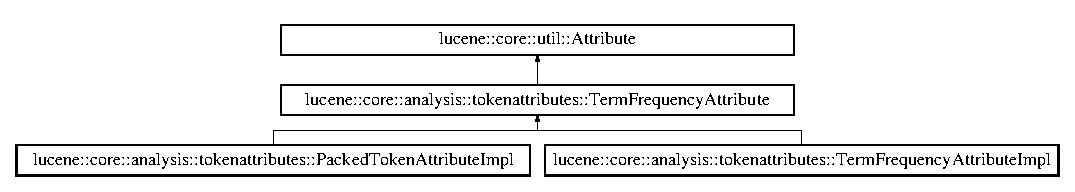
\includegraphics[height=2.137405cm]{classlucene_1_1core_1_1analysis_1_1tokenattributes_1_1TermFrequencyAttribute}
\end{center}
\end{figure}
\subsection*{Public Member Functions}
\begin{DoxyCompactItemize}
\item 
virtual \mbox{\hyperlink{classlucene_1_1core_1_1analysis_1_1tokenattributes_1_1TermFrequencyAttribute_aeb43d01255010bab6bcbf05e74d87d7e}{$\sim$\+Term\+Frequency\+Attribute}} ()
\item 
virtual void \mbox{\hyperlink{classlucene_1_1core_1_1analysis_1_1tokenattributes_1_1TermFrequencyAttribute_aeb8ef8cc3f3ab6c8678b491ac3e1b682}{Set\+Term\+Frequency}} (const uint32\+\_\+t term\+\_\+frequency)=0
\item 
virtual uint32\+\_\+t \mbox{\hyperlink{classlucene_1_1core_1_1analysis_1_1tokenattributes_1_1TermFrequencyAttribute_a2ddffa369215ac61e2eadbab087f5d74}{Get\+Term\+Frequency}} ()=0
\end{DoxyCompactItemize}
\subsection*{Additional Inherited Members}


\subsection{Constructor \& Destructor Documentation}
\mbox{\Hypertarget{classlucene_1_1core_1_1analysis_1_1tokenattributes_1_1TermFrequencyAttribute_aeb43d01255010bab6bcbf05e74d87d7e}\label{classlucene_1_1core_1_1analysis_1_1tokenattributes_1_1TermFrequencyAttribute_aeb43d01255010bab6bcbf05e74d87d7e}} 
\index{lucene\+::core\+::analysis\+::tokenattributes\+::\+Term\+Frequency\+Attribute@{lucene\+::core\+::analysis\+::tokenattributes\+::\+Term\+Frequency\+Attribute}!````~Term\+Frequency\+Attribute@{$\sim$\+Term\+Frequency\+Attribute}}
\index{````~Term\+Frequency\+Attribute@{$\sim$\+Term\+Frequency\+Attribute}!lucene\+::core\+::analysis\+::tokenattributes\+::\+Term\+Frequency\+Attribute@{lucene\+::core\+::analysis\+::tokenattributes\+::\+Term\+Frequency\+Attribute}}
\subsubsection{\texorpdfstring{$\sim$\+Term\+Frequency\+Attribute()}{~TermFrequencyAttribute()}}
{\footnotesize\ttfamily virtual lucene\+::core\+::analysis\+::tokenattributes\+::\+Term\+Frequency\+Attribute\+::$\sim$\+Term\+Frequency\+Attribute (\begin{DoxyParamCaption}{ }\end{DoxyParamCaption})\hspace{0.3cm}{\ttfamily [inline]}, {\ttfamily [virtual]}}



\subsection{Member Function Documentation}
\mbox{\Hypertarget{classlucene_1_1core_1_1analysis_1_1tokenattributes_1_1TermFrequencyAttribute_a2ddffa369215ac61e2eadbab087f5d74}\label{classlucene_1_1core_1_1analysis_1_1tokenattributes_1_1TermFrequencyAttribute_a2ddffa369215ac61e2eadbab087f5d74}} 
\index{lucene\+::core\+::analysis\+::tokenattributes\+::\+Term\+Frequency\+Attribute@{lucene\+::core\+::analysis\+::tokenattributes\+::\+Term\+Frequency\+Attribute}!Get\+Term\+Frequency@{Get\+Term\+Frequency}}
\index{Get\+Term\+Frequency@{Get\+Term\+Frequency}!lucene\+::core\+::analysis\+::tokenattributes\+::\+Term\+Frequency\+Attribute@{lucene\+::core\+::analysis\+::tokenattributes\+::\+Term\+Frequency\+Attribute}}
\subsubsection{\texorpdfstring{Get\+Term\+Frequency()}{GetTermFrequency()}}
{\footnotesize\ttfamily virtual uint32\+\_\+t lucene\+::core\+::analysis\+::tokenattributes\+::\+Term\+Frequency\+Attribute\+::\+Get\+Term\+Frequency (\begin{DoxyParamCaption}{ }\end{DoxyParamCaption})\hspace{0.3cm}{\ttfamily [pure virtual]}}



Implemented in \mbox{\hyperlink{classlucene_1_1core_1_1analysis_1_1tokenattributes_1_1TermFrequencyAttributeImpl_adfd47f9d692a2fbe7a48d590f8c585cb}{lucene\+::core\+::analysis\+::tokenattributes\+::\+Term\+Frequency\+Attribute\+Impl}}, and \mbox{\hyperlink{classlucene_1_1core_1_1analysis_1_1tokenattributes_1_1PackedTokenAttributeImpl_a82aff8ded68bf64ab156382ca6862db2}{lucene\+::core\+::analysis\+::tokenattributes\+::\+Packed\+Token\+Attribute\+Impl}}.

\mbox{\Hypertarget{classlucene_1_1core_1_1analysis_1_1tokenattributes_1_1TermFrequencyAttribute_aeb8ef8cc3f3ab6c8678b491ac3e1b682}\label{classlucene_1_1core_1_1analysis_1_1tokenattributes_1_1TermFrequencyAttribute_aeb8ef8cc3f3ab6c8678b491ac3e1b682}} 
\index{lucene\+::core\+::analysis\+::tokenattributes\+::\+Term\+Frequency\+Attribute@{lucene\+::core\+::analysis\+::tokenattributes\+::\+Term\+Frequency\+Attribute}!Set\+Term\+Frequency@{Set\+Term\+Frequency}}
\index{Set\+Term\+Frequency@{Set\+Term\+Frequency}!lucene\+::core\+::analysis\+::tokenattributes\+::\+Term\+Frequency\+Attribute@{lucene\+::core\+::analysis\+::tokenattributes\+::\+Term\+Frequency\+Attribute}}
\subsubsection{\texorpdfstring{Set\+Term\+Frequency()}{SetTermFrequency()}}
{\footnotesize\ttfamily virtual void lucene\+::core\+::analysis\+::tokenattributes\+::\+Term\+Frequency\+Attribute\+::\+Set\+Term\+Frequency (\begin{DoxyParamCaption}\item[{const uint32\+\_\+t}]{term\+\_\+frequency }\end{DoxyParamCaption})\hspace{0.3cm}{\ttfamily [pure virtual]}}



Implemented in \mbox{\hyperlink{classlucene_1_1core_1_1analysis_1_1tokenattributes_1_1TermFrequencyAttributeImpl_a7662b5bc48f8914a3df96ea22b742e5f}{lucene\+::core\+::analysis\+::tokenattributes\+::\+Term\+Frequency\+Attribute\+Impl}}, and \mbox{\hyperlink{classlucene_1_1core_1_1analysis_1_1tokenattributes_1_1PackedTokenAttributeImpl_a4d9dfc6cc7c825d42789245b8ca003c4}{lucene\+::core\+::analysis\+::tokenattributes\+::\+Packed\+Token\+Attribute\+Impl}}.



The documentation for this class was generated from the following file\+:\begin{DoxyCompactItemize}
\item 
Analysis/\mbox{\hyperlink{Analysis_2Attribute_8h}{Attribute.\+h}}\end{DoxyCompactItemize}

\hypertarget{classlucene_1_1core_1_1analysis_1_1tokenattributes_1_1TermFrequencyAttributeImpl}{}\section{lucene\+:\+:core\+:\+:analysis\+:\+:tokenattributes\+:\+:Term\+Frequency\+Attribute\+Impl Class Reference}
\label{classlucene_1_1core_1_1analysis_1_1tokenattributes_1_1TermFrequencyAttributeImpl}\index{lucene\+::core\+::analysis\+::tokenattributes\+::\+Term\+Frequency\+Attribute\+Impl@{lucene\+::core\+::analysis\+::tokenattributes\+::\+Term\+Frequency\+Attribute\+Impl}}


{\ttfamily \#include $<$Attribute\+Impl.\+h$>$}

Inheritance diagram for lucene\+:\+:core\+:\+:analysis\+:\+:tokenattributes\+:\+:Term\+Frequency\+Attribute\+Impl\+:\begin{figure}[H]
\begin{center}
\leavevmode
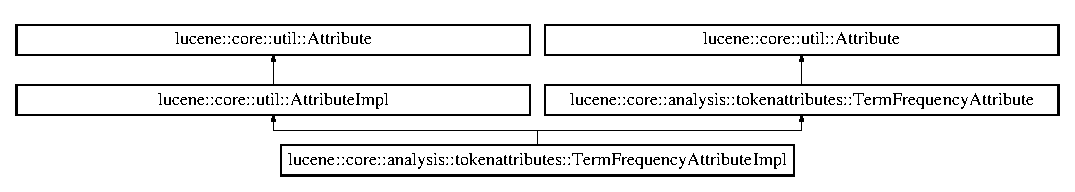
\includegraphics[height=2.137405cm]{classlucene_1_1core_1_1analysis_1_1tokenattributes_1_1TermFrequencyAttributeImpl}
\end{center}
\end{figure}
\subsection*{Public Member Functions}
\begin{DoxyCompactItemize}
\item 
\mbox{\hyperlink{classlucene_1_1core_1_1analysis_1_1tokenattributes_1_1TermFrequencyAttributeImpl_aeda77a35eb6567e63179774e10c1d486}{Term\+Frequency\+Attribute\+Impl}} ()
\item 
\mbox{\hyperlink{classlucene_1_1core_1_1analysis_1_1tokenattributes_1_1TermFrequencyAttributeImpl_a624ed9c4181bde8cca574e75296cde79}{Term\+Frequency\+Attribute\+Impl}} (\mbox{\hyperlink{ZlibCrc32_8h_a2c212835823e3c54a8ab6d95c652660e}{const}} \mbox{\hyperlink{classlucene_1_1core_1_1analysis_1_1tokenattributes_1_1TermFrequencyAttributeImpl}{Term\+Frequency\+Attribute\+Impl}} \&other)
\item 
virtual \mbox{\hyperlink{classlucene_1_1core_1_1analysis_1_1tokenattributes_1_1TermFrequencyAttributeImpl_ad294177d45b1697153b141eddcdecd50}{$\sim$\+Term\+Frequency\+Attribute\+Impl}} ()
\item 
void \mbox{\hyperlink{classlucene_1_1core_1_1analysis_1_1tokenattributes_1_1TermFrequencyAttributeImpl_aef08e2be7b9a57329ed5df12fcb2a9d9}{Reflect\+With}} (\mbox{\hyperlink{namespacelucene_1_1core_1_1util_a7dbb701adaed055f73fb95eec83da10a}{lucene\+::core\+::util\+::\+Attribute\+Reflector}} \&reflector) override
\item 
void \mbox{\hyperlink{classlucene_1_1core_1_1analysis_1_1tokenattributes_1_1TermFrequencyAttributeImpl_aaa575565a7b466b6bdcf4d8042f3f582}{Clear}} () override
\item 
bool \mbox{\hyperlink{classlucene_1_1core_1_1analysis_1_1tokenattributes_1_1TermFrequencyAttributeImpl_aa49e2039c1274b9182bce2c23d52c806}{operator==}} (\mbox{\hyperlink{ZlibCrc32_8h_a2c212835823e3c54a8ab6d95c652660e}{const}} \mbox{\hyperlink{classlucene_1_1core_1_1analysis_1_1tokenattributes_1_1TermFrequencyAttributeImpl}{Term\+Frequency\+Attribute\+Impl}} \&other) \mbox{\hyperlink{ZlibCrc32_8h_a2c212835823e3c54a8ab6d95c652660e}{const}}
\item 
void \mbox{\hyperlink{classlucene_1_1core_1_1analysis_1_1tokenattributes_1_1TermFrequencyAttributeImpl_a7662b5bc48f8914a3df96ea22b742e5f}{Set\+Term\+Frequency}} (\mbox{\hyperlink{ZlibCrc32_8h_a2c212835823e3c54a8ab6d95c652660e}{const}} uint32\+\_\+t \mbox{\hyperlink{classlucene_1_1core_1_1analysis_1_1tokenattributes_1_1TermFrequencyAttributeImpl_a94d743632e8edd5e9e05ce039eec16e8}{term\+\_\+frequency}}) override
\item 
uint32\+\_\+t \mbox{\hyperlink{classlucene_1_1core_1_1analysis_1_1tokenattributes_1_1TermFrequencyAttributeImpl_adfd47f9d692a2fbe7a48d590f8c585cb}{Get\+Term\+Frequency}} () override
\item 
std\+::vector$<$ std\+::type\+\_\+index $>$ \mbox{\hyperlink{classlucene_1_1core_1_1analysis_1_1tokenattributes_1_1TermFrequencyAttributeImpl_a02e08b89bd1105326aff4d578c759886}{Attributes}} () override
\item 
void \mbox{\hyperlink{classlucene_1_1core_1_1analysis_1_1tokenattributes_1_1TermFrequencyAttributeImpl_a82c1cb2877fab77b907b4b03795d0fdf}{Shallow\+Copy\+To}} (\mbox{\hyperlink{classlucene_1_1core_1_1util_1_1AttributeImpl}{lucene\+::core\+::util\+::\+Attribute\+Impl}} \&attr\+\_\+impl) override
\item 
\mbox{\hyperlink{classlucene_1_1core_1_1analysis_1_1tokenattributes_1_1TermFrequencyAttributeImpl}{Term\+Frequency\+Attribute\+Impl}} \& \mbox{\hyperlink{classlucene_1_1core_1_1analysis_1_1tokenattributes_1_1TermFrequencyAttributeImpl_a855437532aa60208023e367fe09926fd}{operator=}} (\mbox{\hyperlink{ZlibCrc32_8h_a2c212835823e3c54a8ab6d95c652660e}{const}} \mbox{\hyperlink{classlucene_1_1core_1_1util_1_1AttributeImpl}{lucene\+::core\+::util\+::\+Attribute\+Impl}} \&other)
\item 
\mbox{\hyperlink{classlucene_1_1core_1_1analysis_1_1tokenattributes_1_1TermFrequencyAttributeImpl}{Term\+Frequency\+Attribute\+Impl}} \& \mbox{\hyperlink{classlucene_1_1core_1_1analysis_1_1tokenattributes_1_1TermFrequencyAttributeImpl_afb31133bdba35cd3e19bbe1aefed9908}{operator=}} (\mbox{\hyperlink{ZlibCrc32_8h_a2c212835823e3c54a8ab6d95c652660e}{const}} \mbox{\hyperlink{classlucene_1_1core_1_1analysis_1_1tokenattributes_1_1TermFrequencyAttributeImpl}{Term\+Frequency\+Attribute\+Impl}} \&other)
\item 
\mbox{\hyperlink{classlucene_1_1core_1_1util_1_1AttributeImpl}{lucene\+::core\+::util\+::\+Attribute\+Impl}} $\ast$ \mbox{\hyperlink{classlucene_1_1core_1_1analysis_1_1tokenattributes_1_1TermFrequencyAttributeImpl_a3d973d479d147e3feece05c9988bc7c6}{Clone}} () override
\end{DoxyCompactItemize}
\subsection*{Private Attributes}
\begin{DoxyCompactItemize}
\item 
uint32\+\_\+t \mbox{\hyperlink{classlucene_1_1core_1_1analysis_1_1tokenattributes_1_1TermFrequencyAttributeImpl_a94d743632e8edd5e9e05ce039eec16e8}{term\+\_\+frequency}}
\end{DoxyCompactItemize}
\subsection*{Additional Inherited Members}


\subsection{Constructor \& Destructor Documentation}
\mbox{\Hypertarget{classlucene_1_1core_1_1analysis_1_1tokenattributes_1_1TermFrequencyAttributeImpl_aeda77a35eb6567e63179774e10c1d486}\label{classlucene_1_1core_1_1analysis_1_1tokenattributes_1_1TermFrequencyAttributeImpl_aeda77a35eb6567e63179774e10c1d486}} 
\index{lucene\+::core\+::analysis\+::tokenattributes\+::\+Term\+Frequency\+Attribute\+Impl@{lucene\+::core\+::analysis\+::tokenattributes\+::\+Term\+Frequency\+Attribute\+Impl}!Term\+Frequency\+Attribute\+Impl@{Term\+Frequency\+Attribute\+Impl}}
\index{Term\+Frequency\+Attribute\+Impl@{Term\+Frequency\+Attribute\+Impl}!lucene\+::core\+::analysis\+::tokenattributes\+::\+Term\+Frequency\+Attribute\+Impl@{lucene\+::core\+::analysis\+::tokenattributes\+::\+Term\+Frequency\+Attribute\+Impl}}
\subsubsection{\texorpdfstring{Term\+Frequency\+Attribute\+Impl()}{TermFrequencyAttributeImpl()}\hspace{0.1cm}{\footnotesize\ttfamily [1/2]}}
{\footnotesize\ttfamily Term\+Frequency\+Attribute\+Impl\+::\+Term\+Frequency\+Attribute\+Impl (\begin{DoxyParamCaption}{ }\end{DoxyParamCaption})}

\mbox{\hyperlink{classlucene_1_1core_1_1analysis_1_1tokenattributes_1_1TermFrequencyAttributeImpl}{Term\+Frequency\+Attribute\+Impl}} \mbox{\Hypertarget{classlucene_1_1core_1_1analysis_1_1tokenattributes_1_1TermFrequencyAttributeImpl_a624ed9c4181bde8cca574e75296cde79}\label{classlucene_1_1core_1_1analysis_1_1tokenattributes_1_1TermFrequencyAttributeImpl_a624ed9c4181bde8cca574e75296cde79}} 
\index{lucene\+::core\+::analysis\+::tokenattributes\+::\+Term\+Frequency\+Attribute\+Impl@{lucene\+::core\+::analysis\+::tokenattributes\+::\+Term\+Frequency\+Attribute\+Impl}!Term\+Frequency\+Attribute\+Impl@{Term\+Frequency\+Attribute\+Impl}}
\index{Term\+Frequency\+Attribute\+Impl@{Term\+Frequency\+Attribute\+Impl}!lucene\+::core\+::analysis\+::tokenattributes\+::\+Term\+Frequency\+Attribute\+Impl@{lucene\+::core\+::analysis\+::tokenattributes\+::\+Term\+Frequency\+Attribute\+Impl}}
\subsubsection{\texorpdfstring{Term\+Frequency\+Attribute\+Impl()}{TermFrequencyAttributeImpl()}\hspace{0.1cm}{\footnotesize\ttfamily [2/2]}}
{\footnotesize\ttfamily Term\+Frequency\+Attribute\+Impl\+::\+Term\+Frequency\+Attribute\+Impl (\begin{DoxyParamCaption}\item[{\mbox{\hyperlink{ZlibCrc32_8h_a2c212835823e3c54a8ab6d95c652660e}{const}} \mbox{\hyperlink{classlucene_1_1core_1_1analysis_1_1tokenattributes_1_1TermFrequencyAttributeImpl}{Term\+Frequency\+Attribute\+Impl}} \&}]{other }\end{DoxyParamCaption})}

\mbox{\Hypertarget{classlucene_1_1core_1_1analysis_1_1tokenattributes_1_1TermFrequencyAttributeImpl_ad294177d45b1697153b141eddcdecd50}\label{classlucene_1_1core_1_1analysis_1_1tokenattributes_1_1TermFrequencyAttributeImpl_ad294177d45b1697153b141eddcdecd50}} 
\index{lucene\+::core\+::analysis\+::tokenattributes\+::\+Term\+Frequency\+Attribute\+Impl@{lucene\+::core\+::analysis\+::tokenattributes\+::\+Term\+Frequency\+Attribute\+Impl}!````~Term\+Frequency\+Attribute\+Impl@{$\sim$\+Term\+Frequency\+Attribute\+Impl}}
\index{````~Term\+Frequency\+Attribute\+Impl@{$\sim$\+Term\+Frequency\+Attribute\+Impl}!lucene\+::core\+::analysis\+::tokenattributes\+::\+Term\+Frequency\+Attribute\+Impl@{lucene\+::core\+::analysis\+::tokenattributes\+::\+Term\+Frequency\+Attribute\+Impl}}
\subsubsection{\texorpdfstring{$\sim$\+Term\+Frequency\+Attribute\+Impl()}{~TermFrequencyAttributeImpl()}}
{\footnotesize\ttfamily Term\+Frequency\+Attribute\+Impl\+::$\sim$\+Term\+Frequency\+Attribute\+Impl (\begin{DoxyParamCaption}{ }\end{DoxyParamCaption})\hspace{0.3cm}{\ttfamily [virtual]}}



\subsection{Member Function Documentation}
\mbox{\Hypertarget{classlucene_1_1core_1_1analysis_1_1tokenattributes_1_1TermFrequencyAttributeImpl_a02e08b89bd1105326aff4d578c759886}\label{classlucene_1_1core_1_1analysis_1_1tokenattributes_1_1TermFrequencyAttributeImpl_a02e08b89bd1105326aff4d578c759886}} 
\index{lucene\+::core\+::analysis\+::tokenattributes\+::\+Term\+Frequency\+Attribute\+Impl@{lucene\+::core\+::analysis\+::tokenattributes\+::\+Term\+Frequency\+Attribute\+Impl}!Attributes@{Attributes}}
\index{Attributes@{Attributes}!lucene\+::core\+::analysis\+::tokenattributes\+::\+Term\+Frequency\+Attribute\+Impl@{lucene\+::core\+::analysis\+::tokenattributes\+::\+Term\+Frequency\+Attribute\+Impl}}
\subsubsection{\texorpdfstring{Attributes()}{Attributes()}}
{\footnotesize\ttfamily std\+::vector$<$ std\+::type\+\_\+index $>$ Term\+Frequency\+Attribute\+Impl\+::\+Attributes (\begin{DoxyParamCaption}{ }\end{DoxyParamCaption})\hspace{0.3cm}{\ttfamily [override]}, {\ttfamily [virtual]}}



Implements \mbox{\hyperlink{classlucene_1_1core_1_1util_1_1AttributeImpl_ac0631e6a7a11044883bc97447716d7cc}{lucene\+::core\+::util\+::\+Attribute\+Impl}}.

\mbox{\Hypertarget{classlucene_1_1core_1_1analysis_1_1tokenattributes_1_1TermFrequencyAttributeImpl_aaa575565a7b466b6bdcf4d8042f3f582}\label{classlucene_1_1core_1_1analysis_1_1tokenattributes_1_1TermFrequencyAttributeImpl_aaa575565a7b466b6bdcf4d8042f3f582}} 
\index{lucene\+::core\+::analysis\+::tokenattributes\+::\+Term\+Frequency\+Attribute\+Impl@{lucene\+::core\+::analysis\+::tokenattributes\+::\+Term\+Frequency\+Attribute\+Impl}!Clear@{Clear}}
\index{Clear@{Clear}!lucene\+::core\+::analysis\+::tokenattributes\+::\+Term\+Frequency\+Attribute\+Impl@{lucene\+::core\+::analysis\+::tokenattributes\+::\+Term\+Frequency\+Attribute\+Impl}}
\subsubsection{\texorpdfstring{Clear()}{Clear()}}
{\footnotesize\ttfamily void Term\+Frequency\+Attribute\+Impl\+::\+Clear (\begin{DoxyParamCaption}{ }\end{DoxyParamCaption})\hspace{0.3cm}{\ttfamily [override]}, {\ttfamily [virtual]}}



Implements \mbox{\hyperlink{classlucene_1_1core_1_1util_1_1AttributeImpl_a04897a00a902f7a345dd44bbc4b482a8}{lucene\+::core\+::util\+::\+Attribute\+Impl}}.

\mbox{\Hypertarget{classlucene_1_1core_1_1analysis_1_1tokenattributes_1_1TermFrequencyAttributeImpl_a3d973d479d147e3feece05c9988bc7c6}\label{classlucene_1_1core_1_1analysis_1_1tokenattributes_1_1TermFrequencyAttributeImpl_a3d973d479d147e3feece05c9988bc7c6}} 
\index{lucene\+::core\+::analysis\+::tokenattributes\+::\+Term\+Frequency\+Attribute\+Impl@{lucene\+::core\+::analysis\+::tokenattributes\+::\+Term\+Frequency\+Attribute\+Impl}!Clone@{Clone}}
\index{Clone@{Clone}!lucene\+::core\+::analysis\+::tokenattributes\+::\+Term\+Frequency\+Attribute\+Impl@{lucene\+::core\+::analysis\+::tokenattributes\+::\+Term\+Frequency\+Attribute\+Impl}}
\subsubsection{\texorpdfstring{Clone()}{Clone()}}
{\footnotesize\ttfamily \mbox{\hyperlink{classlucene_1_1core_1_1util_1_1AttributeImpl}{Attribute\+Impl}} $\ast$ Term\+Frequency\+Attribute\+Impl\+::\+Clone (\begin{DoxyParamCaption}{ }\end{DoxyParamCaption})\hspace{0.3cm}{\ttfamily [override]}, {\ttfamily [virtual]}}



Implements \mbox{\hyperlink{classlucene_1_1core_1_1util_1_1AttributeImpl_a135318ad4c7c17b3d85e625e32fb42cd}{lucene\+::core\+::util\+::\+Attribute\+Impl}}.

\mbox{\Hypertarget{classlucene_1_1core_1_1analysis_1_1tokenattributes_1_1TermFrequencyAttributeImpl_adfd47f9d692a2fbe7a48d590f8c585cb}\label{classlucene_1_1core_1_1analysis_1_1tokenattributes_1_1TermFrequencyAttributeImpl_adfd47f9d692a2fbe7a48d590f8c585cb}} 
\index{lucene\+::core\+::analysis\+::tokenattributes\+::\+Term\+Frequency\+Attribute\+Impl@{lucene\+::core\+::analysis\+::tokenattributes\+::\+Term\+Frequency\+Attribute\+Impl}!Get\+Term\+Frequency@{Get\+Term\+Frequency}}
\index{Get\+Term\+Frequency@{Get\+Term\+Frequency}!lucene\+::core\+::analysis\+::tokenattributes\+::\+Term\+Frequency\+Attribute\+Impl@{lucene\+::core\+::analysis\+::tokenattributes\+::\+Term\+Frequency\+Attribute\+Impl}}
\subsubsection{\texorpdfstring{Get\+Term\+Frequency()}{GetTermFrequency()}}
{\footnotesize\ttfamily uint32\+\_\+t Term\+Frequency\+Attribute\+Impl\+::\+Get\+Term\+Frequency (\begin{DoxyParamCaption}{ }\end{DoxyParamCaption})\hspace{0.3cm}{\ttfamily [override]}, {\ttfamily [virtual]}}



Implements \mbox{\hyperlink{classlucene_1_1core_1_1analysis_1_1tokenattributes_1_1TermFrequencyAttribute_a2ddffa369215ac61e2eadbab087f5d74}{lucene\+::core\+::analysis\+::tokenattributes\+::\+Term\+Frequency\+Attribute}}.

\mbox{\Hypertarget{classlucene_1_1core_1_1analysis_1_1tokenattributes_1_1TermFrequencyAttributeImpl_a855437532aa60208023e367fe09926fd}\label{classlucene_1_1core_1_1analysis_1_1tokenattributes_1_1TermFrequencyAttributeImpl_a855437532aa60208023e367fe09926fd}} 
\index{lucene\+::core\+::analysis\+::tokenattributes\+::\+Term\+Frequency\+Attribute\+Impl@{lucene\+::core\+::analysis\+::tokenattributes\+::\+Term\+Frequency\+Attribute\+Impl}!operator=@{operator=}}
\index{operator=@{operator=}!lucene\+::core\+::analysis\+::tokenattributes\+::\+Term\+Frequency\+Attribute\+Impl@{lucene\+::core\+::analysis\+::tokenattributes\+::\+Term\+Frequency\+Attribute\+Impl}}
\subsubsection{\texorpdfstring{operator=()}{operator=()}\hspace{0.1cm}{\footnotesize\ttfamily [1/2]}}
{\footnotesize\ttfamily \mbox{\hyperlink{classlucene_1_1core_1_1analysis_1_1tokenattributes_1_1TermFrequencyAttributeImpl}{Term\+Frequency\+Attribute\+Impl}} \& Term\+Frequency\+Attribute\+Impl\+::operator= (\begin{DoxyParamCaption}\item[{\mbox{\hyperlink{ZlibCrc32_8h_a2c212835823e3c54a8ab6d95c652660e}{const}} \mbox{\hyperlink{classlucene_1_1core_1_1util_1_1AttributeImpl}{lucene\+::core\+::util\+::\+Attribute\+Impl}} \&}]{other }\end{DoxyParamCaption})\hspace{0.3cm}{\ttfamily [virtual]}}



Implements \mbox{\hyperlink{classlucene_1_1core_1_1util_1_1AttributeImpl_ab032e399d03ce2f58c76881cf2b92325}{lucene\+::core\+::util\+::\+Attribute\+Impl}}.

\mbox{\Hypertarget{classlucene_1_1core_1_1analysis_1_1tokenattributes_1_1TermFrequencyAttributeImpl_afb31133bdba35cd3e19bbe1aefed9908}\label{classlucene_1_1core_1_1analysis_1_1tokenattributes_1_1TermFrequencyAttributeImpl_afb31133bdba35cd3e19bbe1aefed9908}} 
\index{lucene\+::core\+::analysis\+::tokenattributes\+::\+Term\+Frequency\+Attribute\+Impl@{lucene\+::core\+::analysis\+::tokenattributes\+::\+Term\+Frequency\+Attribute\+Impl}!operator=@{operator=}}
\index{operator=@{operator=}!lucene\+::core\+::analysis\+::tokenattributes\+::\+Term\+Frequency\+Attribute\+Impl@{lucene\+::core\+::analysis\+::tokenattributes\+::\+Term\+Frequency\+Attribute\+Impl}}
\subsubsection{\texorpdfstring{operator=()}{operator=()}\hspace{0.1cm}{\footnotesize\ttfamily [2/2]}}
{\footnotesize\ttfamily \mbox{\hyperlink{classlucene_1_1core_1_1analysis_1_1tokenattributes_1_1TermFrequencyAttributeImpl}{Term\+Frequency\+Attribute\+Impl}} \& Term\+Frequency\+Attribute\+Impl\+::operator= (\begin{DoxyParamCaption}\item[{\mbox{\hyperlink{ZlibCrc32_8h_a2c212835823e3c54a8ab6d95c652660e}{const}} \mbox{\hyperlink{classlucene_1_1core_1_1analysis_1_1tokenattributes_1_1TermFrequencyAttributeImpl}{Term\+Frequency\+Attribute\+Impl}} \&}]{other }\end{DoxyParamCaption})}

\mbox{\Hypertarget{classlucene_1_1core_1_1analysis_1_1tokenattributes_1_1TermFrequencyAttributeImpl_aa49e2039c1274b9182bce2c23d52c806}\label{classlucene_1_1core_1_1analysis_1_1tokenattributes_1_1TermFrequencyAttributeImpl_aa49e2039c1274b9182bce2c23d52c806}} 
\index{lucene\+::core\+::analysis\+::tokenattributes\+::\+Term\+Frequency\+Attribute\+Impl@{lucene\+::core\+::analysis\+::tokenattributes\+::\+Term\+Frequency\+Attribute\+Impl}!operator==@{operator==}}
\index{operator==@{operator==}!lucene\+::core\+::analysis\+::tokenattributes\+::\+Term\+Frequency\+Attribute\+Impl@{lucene\+::core\+::analysis\+::tokenattributes\+::\+Term\+Frequency\+Attribute\+Impl}}
\subsubsection{\texorpdfstring{operator==()}{operator==()}}
{\footnotesize\ttfamily bool Term\+Frequency\+Attribute\+Impl\+::operator== (\begin{DoxyParamCaption}\item[{\mbox{\hyperlink{ZlibCrc32_8h_a2c212835823e3c54a8ab6d95c652660e}{const}} \mbox{\hyperlink{classlucene_1_1core_1_1analysis_1_1tokenattributes_1_1TermFrequencyAttributeImpl}{Term\+Frequency\+Attribute\+Impl}} \&}]{other }\end{DoxyParamCaption}) const}

\mbox{\Hypertarget{classlucene_1_1core_1_1analysis_1_1tokenattributes_1_1TermFrequencyAttributeImpl_aef08e2be7b9a57329ed5df12fcb2a9d9}\label{classlucene_1_1core_1_1analysis_1_1tokenattributes_1_1TermFrequencyAttributeImpl_aef08e2be7b9a57329ed5df12fcb2a9d9}} 
\index{lucene\+::core\+::analysis\+::tokenattributes\+::\+Term\+Frequency\+Attribute\+Impl@{lucene\+::core\+::analysis\+::tokenattributes\+::\+Term\+Frequency\+Attribute\+Impl}!Reflect\+With@{Reflect\+With}}
\index{Reflect\+With@{Reflect\+With}!lucene\+::core\+::analysis\+::tokenattributes\+::\+Term\+Frequency\+Attribute\+Impl@{lucene\+::core\+::analysis\+::tokenattributes\+::\+Term\+Frequency\+Attribute\+Impl}}
\subsubsection{\texorpdfstring{Reflect\+With()}{ReflectWith()}}
{\footnotesize\ttfamily void Term\+Frequency\+Attribute\+Impl\+::\+Reflect\+With (\begin{DoxyParamCaption}\item[{\mbox{\hyperlink{namespacelucene_1_1core_1_1util_a7dbb701adaed055f73fb95eec83da10a}{lucene\+::core\+::util\+::\+Attribute\+Reflector}} \&}]{reflector }\end{DoxyParamCaption})\hspace{0.3cm}{\ttfamily [override]}, {\ttfamily [virtual]}}



Implements \mbox{\hyperlink{classlucene_1_1core_1_1util_1_1AttributeImpl_a84d34275fb1ed67ac36fad7ff6388096}{lucene\+::core\+::util\+::\+Attribute\+Impl}}.

\mbox{\Hypertarget{classlucene_1_1core_1_1analysis_1_1tokenattributes_1_1TermFrequencyAttributeImpl_a7662b5bc48f8914a3df96ea22b742e5f}\label{classlucene_1_1core_1_1analysis_1_1tokenattributes_1_1TermFrequencyAttributeImpl_a7662b5bc48f8914a3df96ea22b742e5f}} 
\index{lucene\+::core\+::analysis\+::tokenattributes\+::\+Term\+Frequency\+Attribute\+Impl@{lucene\+::core\+::analysis\+::tokenattributes\+::\+Term\+Frequency\+Attribute\+Impl}!Set\+Term\+Frequency@{Set\+Term\+Frequency}}
\index{Set\+Term\+Frequency@{Set\+Term\+Frequency}!lucene\+::core\+::analysis\+::tokenattributes\+::\+Term\+Frequency\+Attribute\+Impl@{lucene\+::core\+::analysis\+::tokenattributes\+::\+Term\+Frequency\+Attribute\+Impl}}
\subsubsection{\texorpdfstring{Set\+Term\+Frequency()}{SetTermFrequency()}}
{\footnotesize\ttfamily void Term\+Frequency\+Attribute\+Impl\+::\+Set\+Term\+Frequency (\begin{DoxyParamCaption}\item[{\mbox{\hyperlink{ZlibCrc32_8h_a2c212835823e3c54a8ab6d95c652660e}{const}} uint32\+\_\+t}]{term\+\_\+frequency }\end{DoxyParamCaption})\hspace{0.3cm}{\ttfamily [override]}, {\ttfamily [virtual]}}



Implements \mbox{\hyperlink{classlucene_1_1core_1_1analysis_1_1tokenattributes_1_1TermFrequencyAttribute_aeb8ef8cc3f3ab6c8678b491ac3e1b682}{lucene\+::core\+::analysis\+::tokenattributes\+::\+Term\+Frequency\+Attribute}}.

\mbox{\Hypertarget{classlucene_1_1core_1_1analysis_1_1tokenattributes_1_1TermFrequencyAttributeImpl_a82c1cb2877fab77b907b4b03795d0fdf}\label{classlucene_1_1core_1_1analysis_1_1tokenattributes_1_1TermFrequencyAttributeImpl_a82c1cb2877fab77b907b4b03795d0fdf}} 
\index{lucene\+::core\+::analysis\+::tokenattributes\+::\+Term\+Frequency\+Attribute\+Impl@{lucene\+::core\+::analysis\+::tokenattributes\+::\+Term\+Frequency\+Attribute\+Impl}!Shallow\+Copy\+To@{Shallow\+Copy\+To}}
\index{Shallow\+Copy\+To@{Shallow\+Copy\+To}!lucene\+::core\+::analysis\+::tokenattributes\+::\+Term\+Frequency\+Attribute\+Impl@{lucene\+::core\+::analysis\+::tokenattributes\+::\+Term\+Frequency\+Attribute\+Impl}}
\subsubsection{\texorpdfstring{Shallow\+Copy\+To()}{ShallowCopyTo()}}
{\footnotesize\ttfamily void Term\+Frequency\+Attribute\+Impl\+::\+Shallow\+Copy\+To (\begin{DoxyParamCaption}\item[{\mbox{\hyperlink{classlucene_1_1core_1_1util_1_1AttributeImpl}{lucene\+::core\+::util\+::\+Attribute\+Impl}} \&}]{attr\+\_\+impl }\end{DoxyParamCaption})\hspace{0.3cm}{\ttfamily [override]}, {\ttfamily [virtual]}}



Implements \mbox{\hyperlink{classlucene_1_1core_1_1util_1_1AttributeImpl_a010e8937832f53139c8fe42757476895}{lucene\+::core\+::util\+::\+Attribute\+Impl}}.



\subsection{Member Data Documentation}
\mbox{\Hypertarget{classlucene_1_1core_1_1analysis_1_1tokenattributes_1_1TermFrequencyAttributeImpl_a94d743632e8edd5e9e05ce039eec16e8}\label{classlucene_1_1core_1_1analysis_1_1tokenattributes_1_1TermFrequencyAttributeImpl_a94d743632e8edd5e9e05ce039eec16e8}} 
\index{lucene\+::core\+::analysis\+::tokenattributes\+::\+Term\+Frequency\+Attribute\+Impl@{lucene\+::core\+::analysis\+::tokenattributes\+::\+Term\+Frequency\+Attribute\+Impl}!term\+\_\+frequency@{term\+\_\+frequency}}
\index{term\+\_\+frequency@{term\+\_\+frequency}!lucene\+::core\+::analysis\+::tokenattributes\+::\+Term\+Frequency\+Attribute\+Impl@{lucene\+::core\+::analysis\+::tokenattributes\+::\+Term\+Frequency\+Attribute\+Impl}}
\subsubsection{\texorpdfstring{term\+\_\+frequency}{term\_frequency}}
{\footnotesize\ttfamily uint32\+\_\+t lucene\+::core\+::analysis\+::tokenattributes\+::\+Term\+Frequency\+Attribute\+Impl\+::term\+\_\+frequency\hspace{0.3cm}{\ttfamily [private]}}



The documentation for this class was generated from the following files\+:\begin{DoxyCompactItemize}
\item 
Analysis/\mbox{\hyperlink{AttributeImpl_8h}{Attribute\+Impl.\+h}}\item 
Analysis/\mbox{\hyperlink{AttributeImpl_8cpp}{Attribute\+Impl.\+cpp}}\end{DoxyCompactItemize}

\hypertarget{classlucene_1_1core_1_1analysis_1_1tokenattributes_1_1TermToBytesRefAttribute}{}\section{lucene\+:\+:core\+:\+:analysis\+:\+:tokenattributes\+:\+:Term\+To\+Bytes\+Ref\+Attribute Class Reference}
\label{classlucene_1_1core_1_1analysis_1_1tokenattributes_1_1TermToBytesRefAttribute}\index{lucene\+::core\+::analysis\+::tokenattributes\+::\+Term\+To\+Bytes\+Ref\+Attribute@{lucene\+::core\+::analysis\+::tokenattributes\+::\+Term\+To\+Bytes\+Ref\+Attribute}}


{\ttfamily \#include $<$Attribute.\+h$>$}

Inheritance diagram for lucene\+:\+:core\+:\+:analysis\+:\+:tokenattributes\+:\+:Term\+To\+Bytes\+Ref\+Attribute\+:\begin{figure}[H]
\begin{center}
\leavevmode
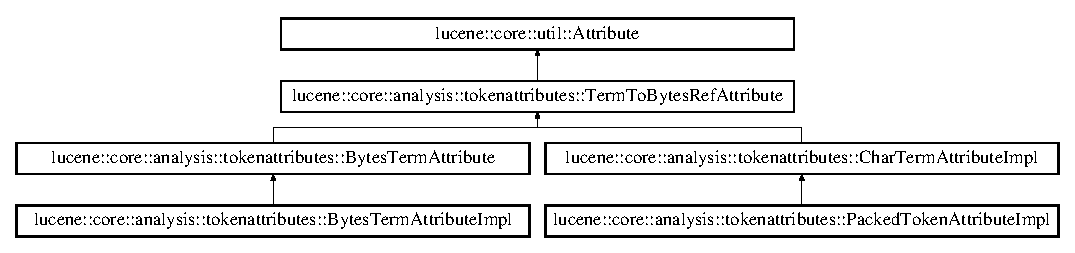
\includegraphics[height=2.947368cm]{classlucene_1_1core_1_1analysis_1_1tokenattributes_1_1TermToBytesRefAttribute}
\end{center}
\end{figure}
\subsection*{Public Member Functions}
\begin{DoxyCompactItemize}
\item 
virtual \mbox{\hyperlink{classlucene_1_1core_1_1analysis_1_1tokenattributes_1_1TermToBytesRefAttribute_aab93d48839ca4330486de269d85d43d7}{$\sim$\+Term\+To\+Bytes\+Ref\+Attribute}} ()
\item 
virtual \mbox{\hyperlink{classlucene_1_1core_1_1util_1_1BytesRef}{lucene\+::core\+::util\+::\+Bytes\+Ref}} \& \mbox{\hyperlink{classlucene_1_1core_1_1analysis_1_1tokenattributes_1_1TermToBytesRefAttribute_a8ae9e4cfc1b97185f8151f3eac76a20d}{Get\+Bytes\+Ref}} ()=0
\end{DoxyCompactItemize}
\subsection*{Additional Inherited Members}


\subsection{Constructor \& Destructor Documentation}
\mbox{\Hypertarget{classlucene_1_1core_1_1analysis_1_1tokenattributes_1_1TermToBytesRefAttribute_aab93d48839ca4330486de269d85d43d7}\label{classlucene_1_1core_1_1analysis_1_1tokenattributes_1_1TermToBytesRefAttribute_aab93d48839ca4330486de269d85d43d7}} 
\index{lucene\+::core\+::analysis\+::tokenattributes\+::\+Term\+To\+Bytes\+Ref\+Attribute@{lucene\+::core\+::analysis\+::tokenattributes\+::\+Term\+To\+Bytes\+Ref\+Attribute}!````~Term\+To\+Bytes\+Ref\+Attribute@{$\sim$\+Term\+To\+Bytes\+Ref\+Attribute}}
\index{````~Term\+To\+Bytes\+Ref\+Attribute@{$\sim$\+Term\+To\+Bytes\+Ref\+Attribute}!lucene\+::core\+::analysis\+::tokenattributes\+::\+Term\+To\+Bytes\+Ref\+Attribute@{lucene\+::core\+::analysis\+::tokenattributes\+::\+Term\+To\+Bytes\+Ref\+Attribute}}
\subsubsection{\texorpdfstring{$\sim$\+Term\+To\+Bytes\+Ref\+Attribute()}{~TermToBytesRefAttribute()}}
{\footnotesize\ttfamily virtual lucene\+::core\+::analysis\+::tokenattributes\+::\+Term\+To\+Bytes\+Ref\+Attribute\+::$\sim$\+Term\+To\+Bytes\+Ref\+Attribute (\begin{DoxyParamCaption}{ }\end{DoxyParamCaption})\hspace{0.3cm}{\ttfamily [inline]}, {\ttfamily [virtual]}}



\subsection{Member Function Documentation}
\mbox{\Hypertarget{classlucene_1_1core_1_1analysis_1_1tokenattributes_1_1TermToBytesRefAttribute_a8ae9e4cfc1b97185f8151f3eac76a20d}\label{classlucene_1_1core_1_1analysis_1_1tokenattributes_1_1TermToBytesRefAttribute_a8ae9e4cfc1b97185f8151f3eac76a20d}} 
\index{lucene\+::core\+::analysis\+::tokenattributes\+::\+Term\+To\+Bytes\+Ref\+Attribute@{lucene\+::core\+::analysis\+::tokenattributes\+::\+Term\+To\+Bytes\+Ref\+Attribute}!Get\+Bytes\+Ref@{Get\+Bytes\+Ref}}
\index{Get\+Bytes\+Ref@{Get\+Bytes\+Ref}!lucene\+::core\+::analysis\+::tokenattributes\+::\+Term\+To\+Bytes\+Ref\+Attribute@{lucene\+::core\+::analysis\+::tokenattributes\+::\+Term\+To\+Bytes\+Ref\+Attribute}}
\subsubsection{\texorpdfstring{Get\+Bytes\+Ref()}{GetBytesRef()}}
{\footnotesize\ttfamily virtual \mbox{\hyperlink{classlucene_1_1core_1_1util_1_1BytesRef}{lucene\+::core\+::util\+::\+Bytes\+Ref}}\& lucene\+::core\+::analysis\+::tokenattributes\+::\+Term\+To\+Bytes\+Ref\+Attribute\+::\+Get\+Bytes\+Ref (\begin{DoxyParamCaption}{ }\end{DoxyParamCaption})\hspace{0.3cm}{\ttfamily [pure virtual]}}



Implemented in \mbox{\hyperlink{classlucene_1_1core_1_1analysis_1_1tokenattributes_1_1CharTermAttributeImpl_aefef8491e2a12493480fe19dd6d61ca7}{lucene\+::core\+::analysis\+::tokenattributes\+::\+Char\+Term\+Attribute\+Impl}}, and \mbox{\hyperlink{classlucene_1_1core_1_1analysis_1_1tokenattributes_1_1BytesTermAttributeImpl_ab0c78ee232b1546b553118afc0117374}{lucene\+::core\+::analysis\+::tokenattributes\+::\+Bytes\+Term\+Attribute\+Impl}}.



The documentation for this class was generated from the following file\+:\begin{DoxyCompactItemize}
\item 
Analysis/\mbox{\hyperlink{Analysis_2Attribute_8h}{Attribute.\+h}}\end{DoxyCompactItemize}

\hypertarget{classlucene_1_1core_1_1util_1_1ThreadLocalItemWrapper}{}\section{lucene\+:\+:core\+:\+:util\+:\+:Thread\+Local\+Item\+Wrapper$<$ T\+Y\+PE $>$ Class Template Reference}
\label{classlucene_1_1core_1_1util_1_1ThreadLocalItemWrapper}\index{lucene\+::core\+::util\+::\+Thread\+Local\+Item\+Wrapper$<$ T\+Y\+P\+E $>$@{lucene\+::core\+::util\+::\+Thread\+Local\+Item\+Wrapper$<$ T\+Y\+P\+E $>$}}


{\ttfamily \#include $<$Concurrency.\+h$>$}

\subsection*{Public Member Functions}
\begin{DoxyCompactItemize}
\item 
\mbox{\hyperlink{classlucene_1_1core_1_1util_1_1ThreadLocalItemWrapper_a22b175e5fd85c3d212bcf35962854add}{Thread\+Local\+Item\+Wrapper}} (\mbox{\hyperlink{classlucene_1_1core_1_1util_1_1ThreadLocalItemWrapper}{Thread\+Local\+Item\+Wrapper}} \&\&other)
\item 
\mbox{\hyperlink{classlucene_1_1core_1_1util_1_1ThreadLocalItemWrapper_aeb556f148918331e663767bf7522d9b6}{Thread\+Local\+Item\+Wrapper}} (\mbox{\hyperlink{ZlibCrc32_8h_a2c212835823e3c54a8ab6d95c652660e}{const}} T\+Y\+PE \&\mbox{\hyperlink{classlucene_1_1core_1_1util_1_1ThreadLocalItemWrapper_ac4814c461c9635ddb4f535f95e0d6cb8}{item}}, bool $\ast$\mbox{\hyperlink{classlucene_1_1core_1_1util_1_1ThreadLocalItemWrapper_a5e0fecb4397f3d5e19a03d07adde08b6}{thread\+\_\+local\+\_\+closed}})
\item 
\mbox{\hyperlink{classlucene_1_1core_1_1util_1_1ThreadLocalItemWrapper_af5f7a927aa01a94971cb9a358488d551}{Thread\+Local\+Item\+Wrapper}} (T\+Y\+PE \&\&\mbox{\hyperlink{classlucene_1_1core_1_1util_1_1ThreadLocalItemWrapper_ac4814c461c9635ddb4f535f95e0d6cb8}{item}}, bool $\ast$\mbox{\hyperlink{classlucene_1_1core_1_1util_1_1ThreadLocalItemWrapper_a5e0fecb4397f3d5e19a03d07adde08b6}{thread\+\_\+local\+\_\+closed}})
\item 
void \mbox{\hyperlink{classlucene_1_1core_1_1util_1_1ThreadLocalItemWrapper_a7ef4309330e9ca0eb7c0b99f19ff1948}{Set\+Closed}} ()
\end{DoxyCompactItemize}
\subsection*{Public Attributes}
\begin{DoxyCompactItemize}
\item 
T\+Y\+PE \mbox{\hyperlink{classlucene_1_1core_1_1util_1_1ThreadLocalItemWrapper_ac4814c461c9635ddb4f535f95e0d6cb8}{item}}
\end{DoxyCompactItemize}
\subsection*{Private Attributes}
\begin{DoxyCompactItemize}
\item 
bool $\ast$ \mbox{\hyperlink{classlucene_1_1core_1_1util_1_1ThreadLocalItemWrapper_a5e0fecb4397f3d5e19a03d07adde08b6}{thread\+\_\+local\+\_\+closed}}
\end{DoxyCompactItemize}


\subsection{Constructor \& Destructor Documentation}
\mbox{\Hypertarget{classlucene_1_1core_1_1util_1_1ThreadLocalItemWrapper_a22b175e5fd85c3d212bcf35962854add}\label{classlucene_1_1core_1_1util_1_1ThreadLocalItemWrapper_a22b175e5fd85c3d212bcf35962854add}} 
\index{lucene\+::core\+::util\+::\+Thread\+Local\+Item\+Wrapper@{lucene\+::core\+::util\+::\+Thread\+Local\+Item\+Wrapper}!Thread\+Local\+Item\+Wrapper@{Thread\+Local\+Item\+Wrapper}}
\index{Thread\+Local\+Item\+Wrapper@{Thread\+Local\+Item\+Wrapper}!lucene\+::core\+::util\+::\+Thread\+Local\+Item\+Wrapper@{lucene\+::core\+::util\+::\+Thread\+Local\+Item\+Wrapper}}
\subsubsection{\texorpdfstring{Thread\+Local\+Item\+Wrapper()}{ThreadLocalItemWrapper()}\hspace{0.1cm}{\footnotesize\ttfamily [1/3]}}
{\footnotesize\ttfamily template$<$typename T\+Y\+PE $>$ \\
\mbox{\hyperlink{classlucene_1_1core_1_1util_1_1ThreadLocalItemWrapper}{lucene\+::core\+::util\+::\+Thread\+Local\+Item\+Wrapper}}$<$ T\+Y\+PE $>$\+::\mbox{\hyperlink{classlucene_1_1core_1_1util_1_1ThreadLocalItemWrapper}{Thread\+Local\+Item\+Wrapper}} (\begin{DoxyParamCaption}\item[{\mbox{\hyperlink{classlucene_1_1core_1_1util_1_1ThreadLocalItemWrapper}{Thread\+Local\+Item\+Wrapper}}$<$ T\+Y\+PE $>$ \&\&}]{other }\end{DoxyParamCaption})\hspace{0.3cm}{\ttfamily [inline]}}

\mbox{\Hypertarget{classlucene_1_1core_1_1util_1_1ThreadLocalItemWrapper_aeb556f148918331e663767bf7522d9b6}\label{classlucene_1_1core_1_1util_1_1ThreadLocalItemWrapper_aeb556f148918331e663767bf7522d9b6}} 
\index{lucene\+::core\+::util\+::\+Thread\+Local\+Item\+Wrapper@{lucene\+::core\+::util\+::\+Thread\+Local\+Item\+Wrapper}!Thread\+Local\+Item\+Wrapper@{Thread\+Local\+Item\+Wrapper}}
\index{Thread\+Local\+Item\+Wrapper@{Thread\+Local\+Item\+Wrapper}!lucene\+::core\+::util\+::\+Thread\+Local\+Item\+Wrapper@{lucene\+::core\+::util\+::\+Thread\+Local\+Item\+Wrapper}}
\subsubsection{\texorpdfstring{Thread\+Local\+Item\+Wrapper()}{ThreadLocalItemWrapper()}\hspace{0.1cm}{\footnotesize\ttfamily [2/3]}}
{\footnotesize\ttfamily template$<$typename T\+Y\+PE $>$ \\
\mbox{\hyperlink{classlucene_1_1core_1_1util_1_1ThreadLocalItemWrapper}{lucene\+::core\+::util\+::\+Thread\+Local\+Item\+Wrapper}}$<$ T\+Y\+PE $>$\+::\mbox{\hyperlink{classlucene_1_1core_1_1util_1_1ThreadLocalItemWrapper}{Thread\+Local\+Item\+Wrapper}} (\begin{DoxyParamCaption}\item[{\mbox{\hyperlink{ZlibCrc32_8h_a2c212835823e3c54a8ab6d95c652660e}{const}} T\+Y\+PE \&}]{item,  }\item[{bool $\ast$}]{thread\+\_\+local\+\_\+closed }\end{DoxyParamCaption})\hspace{0.3cm}{\ttfamily [inline]}}

\mbox{\Hypertarget{classlucene_1_1core_1_1util_1_1ThreadLocalItemWrapper_af5f7a927aa01a94971cb9a358488d551}\label{classlucene_1_1core_1_1util_1_1ThreadLocalItemWrapper_af5f7a927aa01a94971cb9a358488d551}} 
\index{lucene\+::core\+::util\+::\+Thread\+Local\+Item\+Wrapper@{lucene\+::core\+::util\+::\+Thread\+Local\+Item\+Wrapper}!Thread\+Local\+Item\+Wrapper@{Thread\+Local\+Item\+Wrapper}}
\index{Thread\+Local\+Item\+Wrapper@{Thread\+Local\+Item\+Wrapper}!lucene\+::core\+::util\+::\+Thread\+Local\+Item\+Wrapper@{lucene\+::core\+::util\+::\+Thread\+Local\+Item\+Wrapper}}
\subsubsection{\texorpdfstring{Thread\+Local\+Item\+Wrapper()}{ThreadLocalItemWrapper()}\hspace{0.1cm}{\footnotesize\ttfamily [3/3]}}
{\footnotesize\ttfamily template$<$typename T\+Y\+PE $>$ \\
\mbox{\hyperlink{classlucene_1_1core_1_1util_1_1ThreadLocalItemWrapper}{lucene\+::core\+::util\+::\+Thread\+Local\+Item\+Wrapper}}$<$ T\+Y\+PE $>$\+::\mbox{\hyperlink{classlucene_1_1core_1_1util_1_1ThreadLocalItemWrapper}{Thread\+Local\+Item\+Wrapper}} (\begin{DoxyParamCaption}\item[{T\+Y\+PE \&\&}]{item,  }\item[{bool $\ast$}]{thread\+\_\+local\+\_\+closed }\end{DoxyParamCaption})\hspace{0.3cm}{\ttfamily [inline]}}



\subsection{Member Function Documentation}
\mbox{\Hypertarget{classlucene_1_1core_1_1util_1_1ThreadLocalItemWrapper_a7ef4309330e9ca0eb7c0b99f19ff1948}\label{classlucene_1_1core_1_1util_1_1ThreadLocalItemWrapper_a7ef4309330e9ca0eb7c0b99f19ff1948}} 
\index{lucene\+::core\+::util\+::\+Thread\+Local\+Item\+Wrapper@{lucene\+::core\+::util\+::\+Thread\+Local\+Item\+Wrapper}!Set\+Closed@{Set\+Closed}}
\index{Set\+Closed@{Set\+Closed}!lucene\+::core\+::util\+::\+Thread\+Local\+Item\+Wrapper@{lucene\+::core\+::util\+::\+Thread\+Local\+Item\+Wrapper}}
\subsubsection{\texorpdfstring{Set\+Closed()}{SetClosed()}}
{\footnotesize\ttfamily template$<$typename T\+Y\+PE $>$ \\
void \mbox{\hyperlink{classlucene_1_1core_1_1util_1_1ThreadLocalItemWrapper}{lucene\+::core\+::util\+::\+Thread\+Local\+Item\+Wrapper}}$<$ T\+Y\+PE $>$\+::Set\+Closed (\begin{DoxyParamCaption}{ }\end{DoxyParamCaption})\hspace{0.3cm}{\ttfamily [inline]}}



\subsection{Member Data Documentation}
\mbox{\Hypertarget{classlucene_1_1core_1_1util_1_1ThreadLocalItemWrapper_ac4814c461c9635ddb4f535f95e0d6cb8}\label{classlucene_1_1core_1_1util_1_1ThreadLocalItemWrapper_ac4814c461c9635ddb4f535f95e0d6cb8}} 
\index{lucene\+::core\+::util\+::\+Thread\+Local\+Item\+Wrapper@{lucene\+::core\+::util\+::\+Thread\+Local\+Item\+Wrapper}!item@{item}}
\index{item@{item}!lucene\+::core\+::util\+::\+Thread\+Local\+Item\+Wrapper@{lucene\+::core\+::util\+::\+Thread\+Local\+Item\+Wrapper}}
\subsubsection{\texorpdfstring{item}{item}}
{\footnotesize\ttfamily template$<$typename T\+Y\+PE $>$ \\
T\+Y\+PE \mbox{\hyperlink{classlucene_1_1core_1_1util_1_1ThreadLocalItemWrapper}{lucene\+::core\+::util\+::\+Thread\+Local\+Item\+Wrapper}}$<$ T\+Y\+PE $>$\+::item}

\mbox{\Hypertarget{classlucene_1_1core_1_1util_1_1ThreadLocalItemWrapper_a5e0fecb4397f3d5e19a03d07adde08b6}\label{classlucene_1_1core_1_1util_1_1ThreadLocalItemWrapper_a5e0fecb4397f3d5e19a03d07adde08b6}} 
\index{lucene\+::core\+::util\+::\+Thread\+Local\+Item\+Wrapper@{lucene\+::core\+::util\+::\+Thread\+Local\+Item\+Wrapper}!thread\+\_\+local\+\_\+closed@{thread\+\_\+local\+\_\+closed}}
\index{thread\+\_\+local\+\_\+closed@{thread\+\_\+local\+\_\+closed}!lucene\+::core\+::util\+::\+Thread\+Local\+Item\+Wrapper@{lucene\+::core\+::util\+::\+Thread\+Local\+Item\+Wrapper}}
\subsubsection{\texorpdfstring{thread\+\_\+local\+\_\+closed}{thread\_local\_closed}}
{\footnotesize\ttfamily template$<$typename T\+Y\+PE $>$ \\
bool$\ast$ \mbox{\hyperlink{classlucene_1_1core_1_1util_1_1ThreadLocalItemWrapper}{lucene\+::core\+::util\+::\+Thread\+Local\+Item\+Wrapper}}$<$ T\+Y\+PE $>$\+::thread\+\_\+local\+\_\+closed\hspace{0.3cm}{\ttfamily [private]}}



The documentation for this class was generated from the following file\+:\begin{DoxyCompactItemize}
\item 
Util/\mbox{\hyperlink{Concurrency_8h}{Concurrency.\+h}}\end{DoxyCompactItemize}

\hypertarget{classlucene_1_1core_1_1util_1_1ThreadLocalVariableDestructedAlreadyException}{}\section{lucene\+:\+:core\+:\+:util\+:\+:Thread\+Local\+Variable\+Destructed\+Already\+Exception Class Reference}
\label{classlucene_1_1core_1_1util_1_1ThreadLocalVariableDestructedAlreadyException}\index{lucene\+::core\+::util\+::\+Thread\+Local\+Variable\+Destructed\+Already\+Exception@{lucene\+::core\+::util\+::\+Thread\+Local\+Variable\+Destructed\+Already\+Exception}}


{\ttfamily \#include $<$Concurrency.\+h$>$}

Inheritance diagram for lucene\+:\+:core\+:\+:util\+:\+:Thread\+Local\+Variable\+Destructed\+Already\+Exception\+:\begin{figure}[H]
\begin{center}
\leavevmode
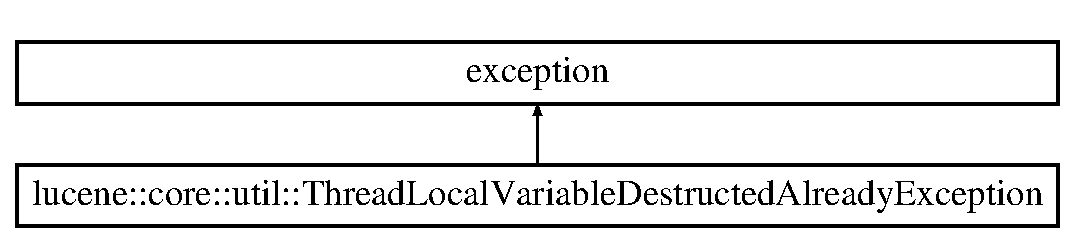
\includegraphics[height=2.000000cm]{classlucene_1_1core_1_1util_1_1ThreadLocalVariableDestructedAlreadyException}
\end{center}
\end{figure}
\subsection*{Public Member Functions}
\begin{DoxyCompactItemize}
\item 
\mbox{\hyperlink{classlucene_1_1core_1_1util_1_1ThreadLocalVariableDestructedAlreadyException_aeead4938bdae97721f6aa94bcdace7a4}{Thread\+Local\+Variable\+Destructed\+Already\+Exception}} ()
\item 
virtual \mbox{\hyperlink{ZlibCrc32_8h_a2c212835823e3c54a8ab6d95c652660e}{const}} char $\ast$ \mbox{\hyperlink{classlucene_1_1core_1_1util_1_1ThreadLocalVariableDestructedAlreadyException_a519acaa7126c57d0c66b1101afa97d38}{what}} () \mbox{\hyperlink{ZlibCrc32_8h_a2c212835823e3c54a8ab6d95c652660e}{const}}  throw ()
\end{DoxyCompactItemize}


\subsection{Constructor \& Destructor Documentation}
\mbox{\Hypertarget{classlucene_1_1core_1_1util_1_1ThreadLocalVariableDestructedAlreadyException_aeead4938bdae97721f6aa94bcdace7a4}\label{classlucene_1_1core_1_1util_1_1ThreadLocalVariableDestructedAlreadyException_aeead4938bdae97721f6aa94bcdace7a4}} 
\index{lucene\+::core\+::util\+::\+Thread\+Local\+Variable\+Destructed\+Already\+Exception@{lucene\+::core\+::util\+::\+Thread\+Local\+Variable\+Destructed\+Already\+Exception}!Thread\+Local\+Variable\+Destructed\+Already\+Exception@{Thread\+Local\+Variable\+Destructed\+Already\+Exception}}
\index{Thread\+Local\+Variable\+Destructed\+Already\+Exception@{Thread\+Local\+Variable\+Destructed\+Already\+Exception}!lucene\+::core\+::util\+::\+Thread\+Local\+Variable\+Destructed\+Already\+Exception@{lucene\+::core\+::util\+::\+Thread\+Local\+Variable\+Destructed\+Already\+Exception}}
\subsubsection{\texorpdfstring{Thread\+Local\+Variable\+Destructed\+Already\+Exception()}{ThreadLocalVariableDestructedAlreadyException()}}
{\footnotesize\ttfamily lucene\+::core\+::util\+::\+Thread\+Local\+Variable\+Destructed\+Already\+Exception\+::\+Thread\+Local\+Variable\+Destructed\+Already\+Exception (\begin{DoxyParamCaption}{ }\end{DoxyParamCaption})\hspace{0.3cm}{\ttfamily [inline]}}



\subsection{Member Function Documentation}
\mbox{\Hypertarget{classlucene_1_1core_1_1util_1_1ThreadLocalVariableDestructedAlreadyException_a519acaa7126c57d0c66b1101afa97d38}\label{classlucene_1_1core_1_1util_1_1ThreadLocalVariableDestructedAlreadyException_a519acaa7126c57d0c66b1101afa97d38}} 
\index{lucene\+::core\+::util\+::\+Thread\+Local\+Variable\+Destructed\+Already\+Exception@{lucene\+::core\+::util\+::\+Thread\+Local\+Variable\+Destructed\+Already\+Exception}!what@{what}}
\index{what@{what}!lucene\+::core\+::util\+::\+Thread\+Local\+Variable\+Destructed\+Already\+Exception@{lucene\+::core\+::util\+::\+Thread\+Local\+Variable\+Destructed\+Already\+Exception}}
\subsubsection{\texorpdfstring{what()}{what()}}
{\footnotesize\ttfamily virtual \mbox{\hyperlink{ZlibCrc32_8h_a2c212835823e3c54a8ab6d95c652660e}{const}} char$\ast$ lucene\+::core\+::util\+::\+Thread\+Local\+Variable\+Destructed\+Already\+Exception\+::what (\begin{DoxyParamCaption}{ }\end{DoxyParamCaption}) const throw  ) \hspace{0.3cm}{\ttfamily [inline]}, {\ttfamily [virtual]}}



The documentation for this class was generated from the following file\+:\begin{DoxyCompactItemize}
\item 
Util/\mbox{\hyperlink{Concurrency_8h}{Concurrency.\+h}}\end{DoxyCompactItemize}

\hypertarget{classlucene_1_1core_1_1analysis_1_1TokenFilter}{}\section{lucene\+:\+:core\+:\+:analysis\+:\+:Token\+Filter Class Reference}
\label{classlucene_1_1core_1_1analysis_1_1TokenFilter}\index{lucene\+::core\+::analysis\+::\+Token\+Filter@{lucene\+::core\+::analysis\+::\+Token\+Filter}}


{\ttfamily \#include $<$Token\+Stream.\+h$>$}

Inheritance diagram for lucene\+:\+:core\+:\+:analysis\+:\+:Token\+Filter\+:\begin{figure}[H]
\begin{center}
\leavevmode
\includegraphics[height=1.413428cm]{classlucene_1_1core_1_1analysis_1_1TokenFilter}
\end{center}
\end{figure}
\subsection*{Public Member Functions}
\begin{DoxyCompactItemize}
\item 
virtual \mbox{\hyperlink{classlucene_1_1core_1_1analysis_1_1TokenFilter_a45308aa10bddc55d4632998ed593be24}{$\sim$\+Token\+Filter}} ()
\item 
void \mbox{\hyperlink{classlucene_1_1core_1_1analysis_1_1TokenFilter_ad2e29dd32aa4df385d0f290f10f20721}{End}} () override
\item 
void \mbox{\hyperlink{classlucene_1_1core_1_1analysis_1_1TokenFilter_a0671ee825db7735a7b72b7a27a457ed9}{Reset}} () override
\item 
void \mbox{\hyperlink{classlucene_1_1core_1_1analysis_1_1TokenFilter_a4b991b01385423b87b5714061e4326c8}{Close}} () override
\item 
{\footnotesize template$<$typename A\+T\+TR $>$ }\\std\+::shared\+\_\+ptr$<$ A\+T\+TR $>$ \mbox{\hyperlink{classlucene_1_1core_1_1analysis_1_1TokenFilter_aea9fad2c3d7b0ae4448653ab5cb3272c}{Add\+Attribute}} ()
\end{DoxyCompactItemize}
\subsection*{Protected Member Functions}
\begin{DoxyCompactItemize}
\item 
\mbox{\hyperlink{classlucene_1_1core_1_1analysis_1_1TokenFilter_af8da6113c95735e58b01f86c42506a17}{Token\+Filter}} (std\+::shared\+\_\+ptr$<$ \mbox{\hyperlink{classlucene_1_1core_1_1analysis_1_1TokenStream}{Token\+Stream}} $>$ \mbox{\hyperlink{classlucene_1_1core_1_1analysis_1_1TokenFilter_aa7b4bf19056c271e00b91a46f2f37504}{input}})
\item 
\mbox{\hyperlink{classlucene_1_1core_1_1analysis_1_1TokenFilter_a0cb8d29a47c80ee2626f8f970d66e4c5}{Token\+Filter}} (\mbox{\hyperlink{classlucene_1_1core_1_1analysis_1_1TokenStream}{Token\+Stream}} $\ast$\mbox{\hyperlink{classlucene_1_1core_1_1analysis_1_1TokenFilter_aa7b4bf19056c271e00b91a46f2f37504}{input}})
\end{DoxyCompactItemize}
\subsection*{Protected Attributes}
\begin{DoxyCompactItemize}
\item 
std\+::shared\+\_\+ptr$<$ \mbox{\hyperlink{classlucene_1_1core_1_1analysis_1_1TokenStream}{Token\+Stream}} $>$ \mbox{\hyperlink{classlucene_1_1core_1_1analysis_1_1TokenFilter_aa7b4bf19056c271e00b91a46f2f37504}{input}}
\end{DoxyCompactItemize}
\subsection*{Additional Inherited Members}


\subsection{Constructor \& Destructor Documentation}
\mbox{\Hypertarget{classlucene_1_1core_1_1analysis_1_1TokenFilter_af8da6113c95735e58b01f86c42506a17}\label{classlucene_1_1core_1_1analysis_1_1TokenFilter_af8da6113c95735e58b01f86c42506a17}} 
\index{lucene\+::core\+::analysis\+::\+Token\+Filter@{lucene\+::core\+::analysis\+::\+Token\+Filter}!Token\+Filter@{Token\+Filter}}
\index{Token\+Filter@{Token\+Filter}!lucene\+::core\+::analysis\+::\+Token\+Filter@{lucene\+::core\+::analysis\+::\+Token\+Filter}}
\subsubsection{\texorpdfstring{Token\+Filter()}{TokenFilter()}\hspace{0.1cm}{\footnotesize\ttfamily [1/2]}}
{\footnotesize\ttfamily Token\+Filter\+::\+Token\+Filter (\begin{DoxyParamCaption}\item[{std\+::shared\+\_\+ptr$<$ \mbox{\hyperlink{classlucene_1_1core_1_1analysis_1_1TokenStream}{Token\+Stream}} $>$}]{input }\end{DoxyParamCaption})\hspace{0.3cm}{\ttfamily [explicit]}, {\ttfamily [protected]}}

\mbox{\hyperlink{classlucene_1_1core_1_1analysis_1_1TokenFilter}{Token\+Filter}} \mbox{\Hypertarget{classlucene_1_1core_1_1analysis_1_1TokenFilter_a0cb8d29a47c80ee2626f8f970d66e4c5}\label{classlucene_1_1core_1_1analysis_1_1TokenFilter_a0cb8d29a47c80ee2626f8f970d66e4c5}} 
\index{lucene\+::core\+::analysis\+::\+Token\+Filter@{lucene\+::core\+::analysis\+::\+Token\+Filter}!Token\+Filter@{Token\+Filter}}
\index{Token\+Filter@{Token\+Filter}!lucene\+::core\+::analysis\+::\+Token\+Filter@{lucene\+::core\+::analysis\+::\+Token\+Filter}}
\subsubsection{\texorpdfstring{Token\+Filter()}{TokenFilter()}\hspace{0.1cm}{\footnotesize\ttfamily [2/2]}}
{\footnotesize\ttfamily Token\+Filter\+::\+Token\+Filter (\begin{DoxyParamCaption}\item[{\mbox{\hyperlink{classlucene_1_1core_1_1analysis_1_1TokenStream}{Token\+Stream}} $\ast$}]{input }\end{DoxyParamCaption})\hspace{0.3cm}{\ttfamily [explicit]}, {\ttfamily [protected]}}

\mbox{\Hypertarget{classlucene_1_1core_1_1analysis_1_1TokenFilter_a45308aa10bddc55d4632998ed593be24}\label{classlucene_1_1core_1_1analysis_1_1TokenFilter_a45308aa10bddc55d4632998ed593be24}} 
\index{lucene\+::core\+::analysis\+::\+Token\+Filter@{lucene\+::core\+::analysis\+::\+Token\+Filter}!````~Token\+Filter@{$\sim$\+Token\+Filter}}
\index{````~Token\+Filter@{$\sim$\+Token\+Filter}!lucene\+::core\+::analysis\+::\+Token\+Filter@{lucene\+::core\+::analysis\+::\+Token\+Filter}}
\subsubsection{\texorpdfstring{$\sim$\+Token\+Filter()}{~TokenFilter()}}
{\footnotesize\ttfamily Token\+Filter\+::$\sim$\+Token\+Filter (\begin{DoxyParamCaption}{ }\end{DoxyParamCaption})\hspace{0.3cm}{\ttfamily [virtual]}}



\subsection{Member Function Documentation}
\mbox{\Hypertarget{classlucene_1_1core_1_1analysis_1_1TokenFilter_aea9fad2c3d7b0ae4448653ab5cb3272c}\label{classlucene_1_1core_1_1analysis_1_1TokenFilter_aea9fad2c3d7b0ae4448653ab5cb3272c}} 
\index{lucene\+::core\+::analysis\+::\+Token\+Filter@{lucene\+::core\+::analysis\+::\+Token\+Filter}!Add\+Attribute@{Add\+Attribute}}
\index{Add\+Attribute@{Add\+Attribute}!lucene\+::core\+::analysis\+::\+Token\+Filter@{lucene\+::core\+::analysis\+::\+Token\+Filter}}
\subsubsection{\texorpdfstring{Add\+Attribute()}{AddAttribute()}}
{\footnotesize\ttfamily template$<$typename A\+T\+TR $>$ \\
std\+::shared\+\_\+ptr$<$A\+T\+TR$>$ lucene\+::core\+::analysis\+::\+Token\+Filter\+::\+Add\+Attribute (\begin{DoxyParamCaption}{ }\end{DoxyParamCaption})\hspace{0.3cm}{\ttfamily [inline]}}

\mbox{\Hypertarget{classlucene_1_1core_1_1analysis_1_1TokenFilter_a4b991b01385423b87b5714061e4326c8}\label{classlucene_1_1core_1_1analysis_1_1TokenFilter_a4b991b01385423b87b5714061e4326c8}} 
\index{lucene\+::core\+::analysis\+::\+Token\+Filter@{lucene\+::core\+::analysis\+::\+Token\+Filter}!Close@{Close}}
\index{Close@{Close}!lucene\+::core\+::analysis\+::\+Token\+Filter@{lucene\+::core\+::analysis\+::\+Token\+Filter}}
\subsubsection{\texorpdfstring{Close()}{Close()}}
{\footnotesize\ttfamily void Token\+Filter\+::\+Close (\begin{DoxyParamCaption}{ }\end{DoxyParamCaption})\hspace{0.3cm}{\ttfamily [override]}, {\ttfamily [virtual]}}



Reimplemented from \mbox{\hyperlink{classlucene_1_1core_1_1analysis_1_1TokenStream_ad7963391ddbb2c75610e3738ba5155c8}{lucene\+::core\+::analysis\+::\+Token\+Stream}}.

\mbox{\Hypertarget{classlucene_1_1core_1_1analysis_1_1TokenFilter_ad2e29dd32aa4df385d0f290f10f20721}\label{classlucene_1_1core_1_1analysis_1_1TokenFilter_ad2e29dd32aa4df385d0f290f10f20721}} 
\index{lucene\+::core\+::analysis\+::\+Token\+Filter@{lucene\+::core\+::analysis\+::\+Token\+Filter}!End@{End}}
\index{End@{End}!lucene\+::core\+::analysis\+::\+Token\+Filter@{lucene\+::core\+::analysis\+::\+Token\+Filter}}
\subsubsection{\texorpdfstring{End()}{End()}}
{\footnotesize\ttfamily void Token\+Filter\+::\+End (\begin{DoxyParamCaption}{ }\end{DoxyParamCaption})\hspace{0.3cm}{\ttfamily [override]}, {\ttfamily [virtual]}}



Reimplemented from \mbox{\hyperlink{classlucene_1_1core_1_1analysis_1_1TokenStream_a4693985ca7fb242412049a074027b8b5}{lucene\+::core\+::analysis\+::\+Token\+Stream}}.



Reimplemented in \mbox{\hyperlink{classlucene_1_1core_1_1analysis_1_1FilteringTokenFilter_adf6b7aac9634afdffe1800a369753688}{lucene\+::core\+::analysis\+::\+Filtering\+Token\+Filter}}, and \mbox{\hyperlink{classlucene_1_1core_1_1analysis_1_1CachingTokenFilter_a7241be5e51e730f4e311572510de147e}{lucene\+::core\+::analysis\+::\+Caching\+Token\+Filter}}.

\mbox{\Hypertarget{classlucene_1_1core_1_1analysis_1_1TokenFilter_a0671ee825db7735a7b72b7a27a457ed9}\label{classlucene_1_1core_1_1analysis_1_1TokenFilter_a0671ee825db7735a7b72b7a27a457ed9}} 
\index{lucene\+::core\+::analysis\+::\+Token\+Filter@{lucene\+::core\+::analysis\+::\+Token\+Filter}!Reset@{Reset}}
\index{Reset@{Reset}!lucene\+::core\+::analysis\+::\+Token\+Filter@{lucene\+::core\+::analysis\+::\+Token\+Filter}}
\subsubsection{\texorpdfstring{Reset()}{Reset()}}
{\footnotesize\ttfamily void Token\+Filter\+::\+Reset (\begin{DoxyParamCaption}{ }\end{DoxyParamCaption})\hspace{0.3cm}{\ttfamily [override]}, {\ttfamily [virtual]}}



Implements \mbox{\hyperlink{classlucene_1_1core_1_1analysis_1_1TokenStream_ae24622f4bc0aeaf0bef924ff1661e023}{lucene\+::core\+::analysis\+::\+Token\+Stream}}.



Reimplemented in \mbox{\hyperlink{classlucene_1_1core_1_1analysis_1_1FilteringTokenFilter_ab85e4deab22d9dedd7ccb7b1f4750400}{lucene\+::core\+::analysis\+::\+Filtering\+Token\+Filter}}, and \mbox{\hyperlink{classlucene_1_1core_1_1analysis_1_1CachingTokenFilter_adde877fb8c464d6eb2766bd400a1499c}{lucene\+::core\+::analysis\+::\+Caching\+Token\+Filter}}.



\subsection{Member Data Documentation}
\mbox{\Hypertarget{classlucene_1_1core_1_1analysis_1_1TokenFilter_aa7b4bf19056c271e00b91a46f2f37504}\label{classlucene_1_1core_1_1analysis_1_1TokenFilter_aa7b4bf19056c271e00b91a46f2f37504}} 
\index{lucene\+::core\+::analysis\+::\+Token\+Filter@{lucene\+::core\+::analysis\+::\+Token\+Filter}!input@{input}}
\index{input@{input}!lucene\+::core\+::analysis\+::\+Token\+Filter@{lucene\+::core\+::analysis\+::\+Token\+Filter}}
\subsubsection{\texorpdfstring{input}{input}}
{\footnotesize\ttfamily std\+::shared\+\_\+ptr$<$\mbox{\hyperlink{classlucene_1_1core_1_1analysis_1_1TokenStream}{Token\+Stream}}$>$ lucene\+::core\+::analysis\+::\+Token\+Filter\+::input\hspace{0.3cm}{\ttfamily [protected]}}



The documentation for this class was generated from the following files\+:\begin{DoxyCompactItemize}
\item 
Analysis/\mbox{\hyperlink{TokenStream_8h}{Token\+Stream.\+h}}\item 
Analysis/\mbox{\hyperlink{TokenStream_8cpp}{Token\+Stream.\+cpp}}\end{DoxyCompactItemize}

\hypertarget{classlucene_1_1core_1_1analysis_1_1Tokenizer}{}\section{lucene\+:\+:core\+:\+:analysis\+:\+:Tokenizer Class Reference}
\label{classlucene_1_1core_1_1analysis_1_1Tokenizer}\index{lucene\+::core\+::analysis\+::\+Tokenizer@{lucene\+::core\+::analysis\+::\+Tokenizer}}


{\ttfamily \#include $<$Token\+Stream.\+h$>$}

Inheritance diagram for lucene\+:\+:core\+:\+:analysis\+:\+:Tokenizer\+:\begin{figure}[H]
\begin{center}
\leavevmode
\includegraphics[height=2.416397cm]{classlucene_1_1core_1_1analysis_1_1Tokenizer}
\end{center}
\end{figure}
\subsection*{Public Member Functions}
\begin{DoxyCompactItemize}
\item 
virtual \mbox{\hyperlink{classlucene_1_1core_1_1analysis_1_1Tokenizer_a3f60f887953edf0f95ba5f36102f7017}{$\sim$\+Tokenizer}} ()
\item 
void \mbox{\hyperlink{classlucene_1_1core_1_1analysis_1_1Tokenizer_a3e5ea6dde1191ef370f42333bda69113}{Set\+Reader}} (\mbox{\hyperlink{classlucene_1_1core_1_1analysis_1_1Reader}{Reader}} \&new\+\_\+input)
\item 
void \mbox{\hyperlink{classlucene_1_1core_1_1analysis_1_1Tokenizer_a459d9c95a28f3b8aa3ad1cfde1568dd3}{Reset}} () override
\item 
void \mbox{\hyperlink{classlucene_1_1core_1_1analysis_1_1Tokenizer_a95c3c0e37e3276be69fa0992b0e45e94}{Close}} ()
\item 
void \mbox{\hyperlink{classlucene_1_1core_1_1analysis_1_1Tokenizer_ad088b90b87896ad88e029f4af370e525}{Set\+Reader\+Test\+Point}} ()
\end{DoxyCompactItemize}
\subsection*{Protected Member Functions}
\begin{DoxyCompactItemize}
\item 
\mbox{\hyperlink{classlucene_1_1core_1_1analysis_1_1Tokenizer_a2a6c04ea8c784f66bebcb6df7073769c}{Tokenizer}} ()
\item 
\mbox{\hyperlink{classlucene_1_1core_1_1analysis_1_1Tokenizer_a88b02b1592e51baa95cd41090183ee8b}{Tokenizer}} (\mbox{\hyperlink{classlucene_1_1core_1_1util_1_1AttributeFactory}{lucene\+::core\+::util\+::\+Attribute\+Factory}} \&\mbox{\hyperlink{classlucene_1_1core_1_1util_1_1AttributeSource_a1376420a752f337a0fdb582bdf160eba}{factory}})
\item 
uint32\+\_\+t \mbox{\hyperlink{classlucene_1_1core_1_1analysis_1_1Tokenizer_a4c10a2cdbd688233cddb87151a8bf168}{Correct\+Offset}} (\mbox{\hyperlink{ZlibCrc32_8h_a2c212835823e3c54a8ab6d95c652660e}{const}} uint32\+\_\+t current\+\_\+off)
\end{DoxyCompactItemize}
\subsection*{Protected Attributes}
\begin{DoxyCompactItemize}
\item 
\mbox{\hyperlink{classlucene_1_1core_1_1analysis_1_1Reader}{Reader}} $\ast$ \mbox{\hyperlink{classlucene_1_1core_1_1analysis_1_1Tokenizer_a376df6bd42b18d1175168b9529b7665e}{input}}
\item 
\mbox{\hyperlink{classlucene_1_1core_1_1analysis_1_1Reader}{Reader}} $\ast$ \mbox{\hyperlink{classlucene_1_1core_1_1analysis_1_1Tokenizer_ac968137c9d44ef57a69c8df4e6e628ff}{input\+\_\+pending}}
\end{DoxyCompactItemize}
\subsection*{Static Private Attributes}
\begin{DoxyCompactItemize}
\item 
static \mbox{\hyperlink{classlucene_1_1core_1_1analysis_1_1IllegalStateReader}{lucene\+::core\+::analysis\+::\+Illegal\+State\+Reader}} \mbox{\hyperlink{classlucene_1_1core_1_1analysis_1_1Tokenizer_a8ddffe6457c8764f4a14326449a42abc}{I\+L\+L\+E\+G\+A\+L\+\_\+\+S\+T\+A\+T\+E\+\_\+\+R\+E\+A\+D\+ER}}
\end{DoxyCompactItemize}
\subsection*{Additional Inherited Members}


\subsection{Constructor \& Destructor Documentation}
\mbox{\Hypertarget{classlucene_1_1core_1_1analysis_1_1Tokenizer_a2a6c04ea8c784f66bebcb6df7073769c}\label{classlucene_1_1core_1_1analysis_1_1Tokenizer_a2a6c04ea8c784f66bebcb6df7073769c}} 
\index{lucene\+::core\+::analysis\+::\+Tokenizer@{lucene\+::core\+::analysis\+::\+Tokenizer}!Tokenizer@{Tokenizer}}
\index{Tokenizer@{Tokenizer}!lucene\+::core\+::analysis\+::\+Tokenizer@{lucene\+::core\+::analysis\+::\+Tokenizer}}
\subsubsection{\texorpdfstring{Tokenizer()}{Tokenizer()}\hspace{0.1cm}{\footnotesize\ttfamily [1/2]}}
{\footnotesize\ttfamily Tokenizer\+::\+Tokenizer (\begin{DoxyParamCaption}{ }\end{DoxyParamCaption})\hspace{0.3cm}{\ttfamily [protected]}}

\mbox{\Hypertarget{classlucene_1_1core_1_1analysis_1_1Tokenizer_a88b02b1592e51baa95cd41090183ee8b}\label{classlucene_1_1core_1_1analysis_1_1Tokenizer_a88b02b1592e51baa95cd41090183ee8b}} 
\index{lucene\+::core\+::analysis\+::\+Tokenizer@{lucene\+::core\+::analysis\+::\+Tokenizer}!Tokenizer@{Tokenizer}}
\index{Tokenizer@{Tokenizer}!lucene\+::core\+::analysis\+::\+Tokenizer@{lucene\+::core\+::analysis\+::\+Tokenizer}}
\subsubsection{\texorpdfstring{Tokenizer()}{Tokenizer()}\hspace{0.1cm}{\footnotesize\ttfamily [2/2]}}
{\footnotesize\ttfamily Tokenizer\+::\+Tokenizer (\begin{DoxyParamCaption}\item[{\mbox{\hyperlink{classlucene_1_1core_1_1util_1_1AttributeFactory}{lucene\+::core\+::util\+::\+Attribute\+Factory}} \&}]{factory }\end{DoxyParamCaption})\hspace{0.3cm}{\ttfamily [explicit]}, {\ttfamily [protected]}}

\mbox{\Hypertarget{classlucene_1_1core_1_1analysis_1_1Tokenizer_a3f60f887953edf0f95ba5f36102f7017}\label{classlucene_1_1core_1_1analysis_1_1Tokenizer_a3f60f887953edf0f95ba5f36102f7017}} 
\index{lucene\+::core\+::analysis\+::\+Tokenizer@{lucene\+::core\+::analysis\+::\+Tokenizer}!````~Tokenizer@{$\sim$\+Tokenizer}}
\index{````~Tokenizer@{$\sim$\+Tokenizer}!lucene\+::core\+::analysis\+::\+Tokenizer@{lucene\+::core\+::analysis\+::\+Tokenizer}}
\subsubsection{\texorpdfstring{$\sim$\+Tokenizer()}{~Tokenizer()}}
{\footnotesize\ttfamily Tokenizer\+::$\sim$\+Tokenizer (\begin{DoxyParamCaption}{ }\end{DoxyParamCaption})\hspace{0.3cm}{\ttfamily [virtual]}}



\subsection{Member Function Documentation}
\mbox{\Hypertarget{classlucene_1_1core_1_1analysis_1_1Tokenizer_a95c3c0e37e3276be69fa0992b0e45e94}\label{classlucene_1_1core_1_1analysis_1_1Tokenizer_a95c3c0e37e3276be69fa0992b0e45e94}} 
\index{lucene\+::core\+::analysis\+::\+Tokenizer@{lucene\+::core\+::analysis\+::\+Tokenizer}!Close@{Close}}
\index{Close@{Close}!lucene\+::core\+::analysis\+::\+Tokenizer@{lucene\+::core\+::analysis\+::\+Tokenizer}}
\subsubsection{\texorpdfstring{Close()}{Close()}}
{\footnotesize\ttfamily void Tokenizer\+::\+Close (\begin{DoxyParamCaption}{ }\end{DoxyParamCaption})\hspace{0.3cm}{\ttfamily [virtual]}}



Reimplemented from \mbox{\hyperlink{classlucene_1_1core_1_1analysis_1_1TokenStream_ad7963391ddbb2c75610e3738ba5155c8}{lucene\+::core\+::analysis\+::\+Token\+Stream}}.

\mbox{\Hypertarget{classlucene_1_1core_1_1analysis_1_1Tokenizer_a4c10a2cdbd688233cddb87151a8bf168}\label{classlucene_1_1core_1_1analysis_1_1Tokenizer_a4c10a2cdbd688233cddb87151a8bf168}} 
\index{lucene\+::core\+::analysis\+::\+Tokenizer@{lucene\+::core\+::analysis\+::\+Tokenizer}!Correct\+Offset@{Correct\+Offset}}
\index{Correct\+Offset@{Correct\+Offset}!lucene\+::core\+::analysis\+::\+Tokenizer@{lucene\+::core\+::analysis\+::\+Tokenizer}}
\subsubsection{\texorpdfstring{Correct\+Offset()}{CorrectOffset()}}
{\footnotesize\ttfamily uint32\+\_\+t Tokenizer\+::\+Correct\+Offset (\begin{DoxyParamCaption}\item[{\mbox{\hyperlink{ZlibCrc32_8h_a2c212835823e3c54a8ab6d95c652660e}{const}} uint32\+\_\+t}]{current\+\_\+off }\end{DoxyParamCaption})\hspace{0.3cm}{\ttfamily [protected]}}

\mbox{\Hypertarget{classlucene_1_1core_1_1analysis_1_1Tokenizer_a459d9c95a28f3b8aa3ad1cfde1568dd3}\label{classlucene_1_1core_1_1analysis_1_1Tokenizer_a459d9c95a28f3b8aa3ad1cfde1568dd3}} 
\index{lucene\+::core\+::analysis\+::\+Tokenizer@{lucene\+::core\+::analysis\+::\+Tokenizer}!Reset@{Reset}}
\index{Reset@{Reset}!lucene\+::core\+::analysis\+::\+Tokenizer@{lucene\+::core\+::analysis\+::\+Tokenizer}}
\subsubsection{\texorpdfstring{Reset()}{Reset()}}
{\footnotesize\ttfamily void Tokenizer\+::\+Reset (\begin{DoxyParamCaption}{ }\end{DoxyParamCaption})\hspace{0.3cm}{\ttfamily [override]}, {\ttfamily [virtual]}}



Implements \mbox{\hyperlink{classlucene_1_1core_1_1analysis_1_1TokenStream_ae24622f4bc0aeaf0bef924ff1661e023}{lucene\+::core\+::analysis\+::\+Token\+Stream}}.

\mbox{\Hypertarget{classlucene_1_1core_1_1analysis_1_1Tokenizer_a3e5ea6dde1191ef370f42333bda69113}\label{classlucene_1_1core_1_1analysis_1_1Tokenizer_a3e5ea6dde1191ef370f42333bda69113}} 
\index{lucene\+::core\+::analysis\+::\+Tokenizer@{lucene\+::core\+::analysis\+::\+Tokenizer}!Set\+Reader@{Set\+Reader}}
\index{Set\+Reader@{Set\+Reader}!lucene\+::core\+::analysis\+::\+Tokenizer@{lucene\+::core\+::analysis\+::\+Tokenizer}}
\subsubsection{\texorpdfstring{Set\+Reader()}{SetReader()}}
{\footnotesize\ttfamily void Tokenizer\+::\+Set\+Reader (\begin{DoxyParamCaption}\item[{\mbox{\hyperlink{classlucene_1_1core_1_1analysis_1_1Reader}{Reader}} \&}]{new\+\_\+input }\end{DoxyParamCaption})}

\mbox{\Hypertarget{classlucene_1_1core_1_1analysis_1_1Tokenizer_ad088b90b87896ad88e029f4af370e525}\label{classlucene_1_1core_1_1analysis_1_1Tokenizer_ad088b90b87896ad88e029f4af370e525}} 
\index{lucene\+::core\+::analysis\+::\+Tokenizer@{lucene\+::core\+::analysis\+::\+Tokenizer}!Set\+Reader\+Test\+Point@{Set\+Reader\+Test\+Point}}
\index{Set\+Reader\+Test\+Point@{Set\+Reader\+Test\+Point}!lucene\+::core\+::analysis\+::\+Tokenizer@{lucene\+::core\+::analysis\+::\+Tokenizer}}
\subsubsection{\texorpdfstring{Set\+Reader\+Test\+Point()}{SetReaderTestPoint()}}
{\footnotesize\ttfamily void Tokenizer\+::\+Set\+Reader\+Test\+Point (\begin{DoxyParamCaption}{ }\end{DoxyParamCaption})}



\subsection{Member Data Documentation}
\mbox{\Hypertarget{classlucene_1_1core_1_1analysis_1_1Tokenizer_a8ddffe6457c8764f4a14326449a42abc}\label{classlucene_1_1core_1_1analysis_1_1Tokenizer_a8ddffe6457c8764f4a14326449a42abc}} 
\index{lucene\+::core\+::analysis\+::\+Tokenizer@{lucene\+::core\+::analysis\+::\+Tokenizer}!I\+L\+L\+E\+G\+A\+L\+\_\+\+S\+T\+A\+T\+E\+\_\+\+R\+E\+A\+D\+ER@{I\+L\+L\+E\+G\+A\+L\+\_\+\+S\+T\+A\+T\+E\+\_\+\+R\+E\+A\+D\+ER}}
\index{I\+L\+L\+E\+G\+A\+L\+\_\+\+S\+T\+A\+T\+E\+\_\+\+R\+E\+A\+D\+ER@{I\+L\+L\+E\+G\+A\+L\+\_\+\+S\+T\+A\+T\+E\+\_\+\+R\+E\+A\+D\+ER}!lucene\+::core\+::analysis\+::\+Tokenizer@{lucene\+::core\+::analysis\+::\+Tokenizer}}
\subsubsection{\texorpdfstring{I\+L\+L\+E\+G\+A\+L\+\_\+\+S\+T\+A\+T\+E\+\_\+\+R\+E\+A\+D\+ER}{ILLEGAL\_STATE\_READER}}
{\footnotesize\ttfamily \mbox{\hyperlink{classlucene_1_1core_1_1analysis_1_1IllegalStateReader}{Illegal\+State\+Reader}} Tokenizer\+::\+I\+L\+L\+E\+G\+A\+L\+\_\+\+S\+T\+A\+T\+E\+\_\+\+R\+E\+A\+D\+ER\hspace{0.3cm}{\ttfamily [static]}, {\ttfamily [private]}}

\mbox{\hyperlink{classlucene_1_1core_1_1analysis_1_1Tokenizer}{Tokenizer}} \mbox{\Hypertarget{classlucene_1_1core_1_1analysis_1_1Tokenizer_a376df6bd42b18d1175168b9529b7665e}\label{classlucene_1_1core_1_1analysis_1_1Tokenizer_a376df6bd42b18d1175168b9529b7665e}} 
\index{lucene\+::core\+::analysis\+::\+Tokenizer@{lucene\+::core\+::analysis\+::\+Tokenizer}!input@{input}}
\index{input@{input}!lucene\+::core\+::analysis\+::\+Tokenizer@{lucene\+::core\+::analysis\+::\+Tokenizer}}
\subsubsection{\texorpdfstring{input}{input}}
{\footnotesize\ttfamily \mbox{\hyperlink{classlucene_1_1core_1_1analysis_1_1Reader}{Reader}}$\ast$ lucene\+::core\+::analysis\+::\+Tokenizer\+::input\hspace{0.3cm}{\ttfamily [protected]}}

\mbox{\Hypertarget{classlucene_1_1core_1_1analysis_1_1Tokenizer_ac968137c9d44ef57a69c8df4e6e628ff}\label{classlucene_1_1core_1_1analysis_1_1Tokenizer_ac968137c9d44ef57a69c8df4e6e628ff}} 
\index{lucene\+::core\+::analysis\+::\+Tokenizer@{lucene\+::core\+::analysis\+::\+Tokenizer}!input\+\_\+pending@{input\+\_\+pending}}
\index{input\+\_\+pending@{input\+\_\+pending}!lucene\+::core\+::analysis\+::\+Tokenizer@{lucene\+::core\+::analysis\+::\+Tokenizer}}
\subsubsection{\texorpdfstring{input\+\_\+pending}{input\_pending}}
{\footnotesize\ttfamily \mbox{\hyperlink{classlucene_1_1core_1_1analysis_1_1Reader}{Reader}}$\ast$ lucene\+::core\+::analysis\+::\+Tokenizer\+::input\+\_\+pending\hspace{0.3cm}{\ttfamily [protected]}}



The documentation for this class was generated from the following files\+:\begin{DoxyCompactItemize}
\item 
Analysis/\mbox{\hyperlink{TokenStream_8h}{Token\+Stream.\+h}}\item 
Analysis/\mbox{\hyperlink{TokenStream_8cpp}{Token\+Stream.\+cpp}}\end{DoxyCompactItemize}

\hypertarget{classlucene_1_1core_1_1analysis_1_1TokenStream}{}\section{lucene\+:\+:core\+:\+:analysis\+:\+:Token\+Stream Class Reference}
\label{classlucene_1_1core_1_1analysis_1_1TokenStream}\index{lucene\+::core\+::analysis\+::\+Token\+Stream@{lucene\+::core\+::analysis\+::\+Token\+Stream}}


{\ttfamily \#include $<$Token\+Stream.\+h$>$}

Inheritance diagram for lucene\+:\+:core\+:\+:analysis\+:\+:Token\+Stream\+:\begin{figure}[H]
\begin{center}
\leavevmode
\includegraphics[height=3.020496cm]{classlucene_1_1core_1_1analysis_1_1TokenStream}
\end{center}
\end{figure}
\subsection*{Public Member Functions}
\begin{DoxyCompactItemize}
\item 
virtual \mbox{\hyperlink{classlucene_1_1core_1_1analysis_1_1TokenStream_a16519782e35e74b26236c729c6b94f8c}{$\sim$\+Token\+Stream}} ()
\item 
virtual bool \mbox{\hyperlink{classlucene_1_1core_1_1analysis_1_1TokenStream_a614d4ea24a354d6f4354b4941b5124e2}{Increment\+Token}} ()=0
\item 
virtual void \mbox{\hyperlink{classlucene_1_1core_1_1analysis_1_1TokenStream_a4693985ca7fb242412049a074027b8b5}{End}} ()
\item 
virtual void \mbox{\hyperlink{classlucene_1_1core_1_1analysis_1_1TokenStream_ae24622f4bc0aeaf0bef924ff1661e023}{Reset}} ()=0
\item 
virtual void \mbox{\hyperlink{classlucene_1_1core_1_1analysis_1_1TokenStream_ad7963391ddbb2c75610e3738ba5155c8}{Close}} ()
\end{DoxyCompactItemize}
\subsection*{Static Public Attributes}
\begin{DoxyCompactItemize}
\item 
static \mbox{\hyperlink{classlucene_1_1core_1_1util_1_1AttributeFactory}{lucene\+::core\+::util\+::\+Attribute\+Factory}} $\ast$ \mbox{\hyperlink{classlucene_1_1core_1_1analysis_1_1TokenStream_a3a38785c7907943994326cb9d7180671}{D\+E\+F\+A\+U\+L\+T\+\_\+\+T\+O\+K\+E\+N\+\_\+\+A\+T\+T\+R\+I\+B\+U\+T\+E\+\_\+\+F\+A\+C\+T\+O\+RY}}
\end{DoxyCompactItemize}
\subsection*{Protected Member Functions}
\begin{DoxyCompactItemize}
\item 
\mbox{\hyperlink{classlucene_1_1core_1_1analysis_1_1TokenStream_aa9190a1864f989c530aa6c470750d2d8}{Token\+Stream}} ()
\item 
\mbox{\hyperlink{classlucene_1_1core_1_1analysis_1_1TokenStream_a225edeafcbb8da438c1e4ce156357bb6}{Token\+Stream}} (const \mbox{\hyperlink{classlucene_1_1core_1_1util_1_1AttributeSource}{lucene\+::core\+::util\+::\+Attribute\+Source}} \&input)
\item 
\mbox{\hyperlink{classlucene_1_1core_1_1analysis_1_1TokenStream_ae8358809645d3dff705d514cac50ea17}{Token\+Stream}} (\mbox{\hyperlink{classlucene_1_1core_1_1util_1_1AttributeFactory}{lucene\+::core\+::util\+::\+Attribute\+Factory}} \&\mbox{\hyperlink{classlucene_1_1core_1_1util_1_1AttributeSource_a1376420a752f337a0fdb582bdf160eba}{factory}})
\end{DoxyCompactItemize}


\subsection{Constructor \& Destructor Documentation}
\mbox{\Hypertarget{classlucene_1_1core_1_1analysis_1_1TokenStream_aa9190a1864f989c530aa6c470750d2d8}\label{classlucene_1_1core_1_1analysis_1_1TokenStream_aa9190a1864f989c530aa6c470750d2d8}} 
\index{lucene\+::core\+::analysis\+::\+Token\+Stream@{lucene\+::core\+::analysis\+::\+Token\+Stream}!Token\+Stream@{Token\+Stream}}
\index{Token\+Stream@{Token\+Stream}!lucene\+::core\+::analysis\+::\+Token\+Stream@{lucene\+::core\+::analysis\+::\+Token\+Stream}}
\subsubsection{\texorpdfstring{Token\+Stream()}{TokenStream()}\hspace{0.1cm}{\footnotesize\ttfamily [1/3]}}
{\footnotesize\ttfamily Token\+Stream\+::\+Token\+Stream (\begin{DoxyParamCaption}{ }\end{DoxyParamCaption})\hspace{0.3cm}{\ttfamily [protected]}}

\mbox{\Hypertarget{classlucene_1_1core_1_1analysis_1_1TokenStream_a225edeafcbb8da438c1e4ce156357bb6}\label{classlucene_1_1core_1_1analysis_1_1TokenStream_a225edeafcbb8da438c1e4ce156357bb6}} 
\index{lucene\+::core\+::analysis\+::\+Token\+Stream@{lucene\+::core\+::analysis\+::\+Token\+Stream}!Token\+Stream@{Token\+Stream}}
\index{Token\+Stream@{Token\+Stream}!lucene\+::core\+::analysis\+::\+Token\+Stream@{lucene\+::core\+::analysis\+::\+Token\+Stream}}
\subsubsection{\texorpdfstring{Token\+Stream()}{TokenStream()}\hspace{0.1cm}{\footnotesize\ttfamily [2/3]}}
{\footnotesize\ttfamily lucene\+::core\+::analysis\+::\+Token\+Stream\+::\+Token\+Stream (\begin{DoxyParamCaption}\item[{const \mbox{\hyperlink{classlucene_1_1core_1_1util_1_1AttributeSource}{lucene\+::core\+::util\+::\+Attribute\+Source}} \&}]{input }\end{DoxyParamCaption})\hspace{0.3cm}{\ttfamily [explicit]}, {\ttfamily [protected]}}

\mbox{\Hypertarget{classlucene_1_1core_1_1analysis_1_1TokenStream_ae8358809645d3dff705d514cac50ea17}\label{classlucene_1_1core_1_1analysis_1_1TokenStream_ae8358809645d3dff705d514cac50ea17}} 
\index{lucene\+::core\+::analysis\+::\+Token\+Stream@{lucene\+::core\+::analysis\+::\+Token\+Stream}!Token\+Stream@{Token\+Stream}}
\index{Token\+Stream@{Token\+Stream}!lucene\+::core\+::analysis\+::\+Token\+Stream@{lucene\+::core\+::analysis\+::\+Token\+Stream}}
\subsubsection{\texorpdfstring{Token\+Stream()}{TokenStream()}\hspace{0.1cm}{\footnotesize\ttfamily [3/3]}}
{\footnotesize\ttfamily Token\+Stream\+::\+Token\+Stream (\begin{DoxyParamCaption}\item[{\mbox{\hyperlink{classlucene_1_1core_1_1util_1_1AttributeFactory}{lucene\+::core\+::util\+::\+Attribute\+Factory}} \&}]{factory }\end{DoxyParamCaption})\hspace{0.3cm}{\ttfamily [explicit]}, {\ttfamily [protected]}}

\mbox{\Hypertarget{classlucene_1_1core_1_1analysis_1_1TokenStream_a16519782e35e74b26236c729c6b94f8c}\label{classlucene_1_1core_1_1analysis_1_1TokenStream_a16519782e35e74b26236c729c6b94f8c}} 
\index{lucene\+::core\+::analysis\+::\+Token\+Stream@{lucene\+::core\+::analysis\+::\+Token\+Stream}!````~Token\+Stream@{$\sim$\+Token\+Stream}}
\index{````~Token\+Stream@{$\sim$\+Token\+Stream}!lucene\+::core\+::analysis\+::\+Token\+Stream@{lucene\+::core\+::analysis\+::\+Token\+Stream}}
\subsubsection{\texorpdfstring{$\sim$\+Token\+Stream()}{~TokenStream()}}
{\footnotesize\ttfamily Token\+Stream\+::$\sim$\+Token\+Stream (\begin{DoxyParamCaption}{ }\end{DoxyParamCaption})\hspace{0.3cm}{\ttfamily [virtual]}}



\subsection{Member Function Documentation}
\mbox{\Hypertarget{classlucene_1_1core_1_1analysis_1_1TokenStream_ad7963391ddbb2c75610e3738ba5155c8}\label{classlucene_1_1core_1_1analysis_1_1TokenStream_ad7963391ddbb2c75610e3738ba5155c8}} 
\index{lucene\+::core\+::analysis\+::\+Token\+Stream@{lucene\+::core\+::analysis\+::\+Token\+Stream}!Close@{Close}}
\index{Close@{Close}!lucene\+::core\+::analysis\+::\+Token\+Stream@{lucene\+::core\+::analysis\+::\+Token\+Stream}}
\subsubsection{\texorpdfstring{Close()}{Close()}}
{\footnotesize\ttfamily void Token\+Stream\+::\+Close (\begin{DoxyParamCaption}{ }\end{DoxyParamCaption})\hspace{0.3cm}{\ttfamily [virtual]}}



Reimplemented in \mbox{\hyperlink{classlucene_1_1core_1_1document_1_1Field_1_1StringTokenStream_acbf15ee849ed8055143c77b96f116cf0}{lucene\+::core\+::document\+::\+Field\+::\+String\+Token\+Stream}}, \mbox{\hyperlink{classlucene_1_1core_1_1document_1_1Field_1_1BinaryTokenStream_a44c200cf1139a926308afdcf27c7638d}{lucene\+::core\+::document\+::\+Field\+::\+Binary\+Token\+Stream}}, \mbox{\hyperlink{classlucene_1_1core_1_1analysis_1_1standard_1_1StandardTokenizer_a108793659fb18bdd695e0c2be91ba730}{lucene\+::core\+::analysis\+::standard\+::\+Standard\+Tokenizer}}, \mbox{\hyperlink{classlucene_1_1core_1_1analysis_1_1Tokenizer_a95c3c0e37e3276be69fa0992b0e45e94}{lucene\+::core\+::analysis\+::\+Tokenizer}}, and \mbox{\hyperlink{classlucene_1_1core_1_1analysis_1_1TokenFilter_a4b991b01385423b87b5714061e4326c8}{lucene\+::core\+::analysis\+::\+Token\+Filter}}.

\mbox{\Hypertarget{classlucene_1_1core_1_1analysis_1_1TokenStream_a4693985ca7fb242412049a074027b8b5}\label{classlucene_1_1core_1_1analysis_1_1TokenStream_a4693985ca7fb242412049a074027b8b5}} 
\index{lucene\+::core\+::analysis\+::\+Token\+Stream@{lucene\+::core\+::analysis\+::\+Token\+Stream}!End@{End}}
\index{End@{End}!lucene\+::core\+::analysis\+::\+Token\+Stream@{lucene\+::core\+::analysis\+::\+Token\+Stream}}
\subsubsection{\texorpdfstring{End()}{End()}}
{\footnotesize\ttfamily void Token\+Stream\+::\+End (\begin{DoxyParamCaption}{ }\end{DoxyParamCaption})\hspace{0.3cm}{\ttfamily [virtual]}}



Reimplemented in \mbox{\hyperlink{classlucene_1_1core_1_1document_1_1Field_1_1StringTokenStream_acbadfa77de855b030af35f1206231525}{lucene\+::core\+::document\+::\+Field\+::\+String\+Token\+Stream}}, \mbox{\hyperlink{classlucene_1_1core_1_1analysis_1_1FilteringTokenFilter_adf6b7aac9634afdffe1800a369753688}{lucene\+::core\+::analysis\+::\+Filtering\+Token\+Filter}}, \mbox{\hyperlink{classlucene_1_1core_1_1analysis_1_1CachingTokenFilter_a7241be5e51e730f4e311572510de147e}{lucene\+::core\+::analysis\+::\+Caching\+Token\+Filter}}, \mbox{\hyperlink{classlucene_1_1core_1_1analysis_1_1standard_1_1StandardTokenizer_a733b678af865ff10e41fba9b74131872}{lucene\+::core\+::analysis\+::standard\+::\+Standard\+Tokenizer}}, \mbox{\hyperlink{classlucene_1_1core_1_1analysis_1_1StringTokenStream_aabf9a873c934aff5c359417488f33849}{lucene\+::core\+::analysis\+::\+String\+Token\+Stream}}, \mbox{\hyperlink{classlucene_1_1core_1_1analysis_1_1TokenFilter_ad2e29dd32aa4df385d0f290f10f20721}{lucene\+::core\+::analysis\+::\+Token\+Filter}}, and \mbox{\hyperlink{classNaiveWhiteSpaceTokenizer_a4c4f4debc08aa3e05b07b782144b5ae6}{Naive\+White\+Space\+Tokenizer}}.

\mbox{\Hypertarget{classlucene_1_1core_1_1analysis_1_1TokenStream_a614d4ea24a354d6f4354b4941b5124e2}\label{classlucene_1_1core_1_1analysis_1_1TokenStream_a614d4ea24a354d6f4354b4941b5124e2}} 
\index{lucene\+::core\+::analysis\+::\+Token\+Stream@{lucene\+::core\+::analysis\+::\+Token\+Stream}!Increment\+Token@{Increment\+Token}}
\index{Increment\+Token@{Increment\+Token}!lucene\+::core\+::analysis\+::\+Token\+Stream@{lucene\+::core\+::analysis\+::\+Token\+Stream}}
\subsubsection{\texorpdfstring{Increment\+Token()}{IncrementToken()}}
{\footnotesize\ttfamily virtual bool lucene\+::core\+::analysis\+::\+Token\+Stream\+::\+Increment\+Token (\begin{DoxyParamCaption}{ }\end{DoxyParamCaption})\hspace{0.3cm}{\ttfamily [pure virtual]}}



Implemented in \mbox{\hyperlink{classlucene_1_1core_1_1document_1_1Field_1_1StringTokenStream_a161893ca5de24e392426fea5999334fb}{lucene\+::core\+::document\+::\+Field\+::\+String\+Token\+Stream}}, \mbox{\hyperlink{classlucene_1_1core_1_1document_1_1Field_1_1BinaryTokenStream_a98dee5401b26bdaab935f66a37abae29}{lucene\+::core\+::document\+::\+Field\+::\+Binary\+Token\+Stream}}, \mbox{\hyperlink{classlucene_1_1core_1_1analysis_1_1FilteringTokenFilter_aa1956aa94779023b3f97b667bd819734}{lucene\+::core\+::analysis\+::\+Filtering\+Token\+Filter}}, \mbox{\hyperlink{classlucene_1_1core_1_1analysis_1_1CachingTokenFilter_acea0a0a5ee61ab8831209c96fde49dc8}{lucene\+::core\+::analysis\+::\+Caching\+Token\+Filter}}, \mbox{\hyperlink{classTransparentTokenFilter_ae0bc79516b4f3fae3af29a9d05b4acf6}{Transparent\+Token\+Filter}}, \mbox{\hyperlink{classlucene_1_1core_1_1analysis_1_1standard_1_1StandardTokenizer_a5702119d01489ede9396db0794a98c41}{lucene\+::core\+::analysis\+::standard\+::\+Standard\+Tokenizer}}, \mbox{\hyperlink{classlucene_1_1core_1_1analysis_1_1LowerCaseFilter_a0e32bf7c330bccfb7ad3c68a374683a7}{lucene\+::core\+::analysis\+::\+Lower\+Case\+Filter}}, \mbox{\hyperlink{classHateThreeWordsTokenFilter_ad843fcf23da10776311702c619c02560}{Hate\+Three\+Words\+Token\+Filter}}, \mbox{\hyperlink{classDummyTokenFilter_a6a57ec2684cc58f61ec807bbebabae63}{Dummy\+Token\+Filter}}, \mbox{\hyperlink{classlucene_1_1core_1_1analysis_1_1StringTokenStream_a059da09c86bcf50a286803cad1b99d10}{lucene\+::core\+::analysis\+::\+String\+Token\+Stream}}, \mbox{\hyperlink{classNaiveWhiteSpaceTokenizer_aa1dcc35eedacdb6107441cb9010d60b0}{Naive\+White\+Space\+Tokenizer}}, \mbox{\hyperlink{classlucene_1_1core_1_1analysis_1_1standard_1_1StandardFilter_a11958d89cb4aed281d083db7be0e8680}{lucene\+::core\+::analysis\+::standard\+::\+Standard\+Filter}}, and \mbox{\hyperlink{classDummyTokenizer_a11402de15d04027b30ce918814e1723d}{Dummy\+Tokenizer}}.

\mbox{\Hypertarget{classlucene_1_1core_1_1analysis_1_1TokenStream_ae24622f4bc0aeaf0bef924ff1661e023}\label{classlucene_1_1core_1_1analysis_1_1TokenStream_ae24622f4bc0aeaf0bef924ff1661e023}} 
\index{lucene\+::core\+::analysis\+::\+Token\+Stream@{lucene\+::core\+::analysis\+::\+Token\+Stream}!Reset@{Reset}}
\index{Reset@{Reset}!lucene\+::core\+::analysis\+::\+Token\+Stream@{lucene\+::core\+::analysis\+::\+Token\+Stream}}
\subsubsection{\texorpdfstring{Reset()}{Reset()}}
{\footnotesize\ttfamily virtual void lucene\+::core\+::analysis\+::\+Token\+Stream\+::\+Reset (\begin{DoxyParamCaption}{ }\end{DoxyParamCaption})\hspace{0.3cm}{\ttfamily [pure virtual]}}



Implemented in \mbox{\hyperlink{classlucene_1_1core_1_1document_1_1Field_1_1StringTokenStream_ac0073673de4b2eb307408d1aee40625c}{lucene\+::core\+::document\+::\+Field\+::\+String\+Token\+Stream}}, \mbox{\hyperlink{classlucene_1_1core_1_1document_1_1Field_1_1BinaryTokenStream_a99e2c5a8f41c6509ae7a43ade13c30bf}{lucene\+::core\+::document\+::\+Field\+::\+Binary\+Token\+Stream}}, \mbox{\hyperlink{classlucene_1_1core_1_1analysis_1_1FilteringTokenFilter_ab85e4deab22d9dedd7ccb7b1f4750400}{lucene\+::core\+::analysis\+::\+Filtering\+Token\+Filter}}, \mbox{\hyperlink{classlucene_1_1core_1_1analysis_1_1CachingTokenFilter_adde877fb8c464d6eb2766bd400a1499c}{lucene\+::core\+::analysis\+::\+Caching\+Token\+Filter}}, \mbox{\hyperlink{classlucene_1_1core_1_1analysis_1_1standard_1_1StandardTokenizer_a4d6e42ca0fcaf07cb6615643362891b3}{lucene\+::core\+::analysis\+::standard\+::\+Standard\+Tokenizer}}, \mbox{\hyperlink{classlucene_1_1core_1_1analysis_1_1Tokenizer_a459d9c95a28f3b8aa3ad1cfde1568dd3}{lucene\+::core\+::analysis\+::\+Tokenizer}}, \mbox{\hyperlink{classlucene_1_1core_1_1analysis_1_1StringTokenStream_ab578e75921eb1757b4a8887cf29fe94d}{lucene\+::core\+::analysis\+::\+String\+Token\+Stream}}, \mbox{\hyperlink{classlucene_1_1core_1_1analysis_1_1TokenFilter_a0671ee825db7735a7b72b7a27a457ed9}{lucene\+::core\+::analysis\+::\+Token\+Filter}}, and \mbox{\hyperlink{classNaiveWhiteSpaceTokenizer_aa532e6a3e2fa6a9ebb90a4324179a30f}{Naive\+White\+Space\+Tokenizer}}.



\subsection{Member Data Documentation}
\mbox{\Hypertarget{classlucene_1_1core_1_1analysis_1_1TokenStream_a3a38785c7907943994326cb9d7180671}\label{classlucene_1_1core_1_1analysis_1_1TokenStream_a3a38785c7907943994326cb9d7180671}} 
\index{lucene\+::core\+::analysis\+::\+Token\+Stream@{lucene\+::core\+::analysis\+::\+Token\+Stream}!D\+E\+F\+A\+U\+L\+T\+\_\+\+T\+O\+K\+E\+N\+\_\+\+A\+T\+T\+R\+I\+B\+U\+T\+E\+\_\+\+F\+A\+C\+T\+O\+RY@{D\+E\+F\+A\+U\+L\+T\+\_\+\+T\+O\+K\+E\+N\+\_\+\+A\+T\+T\+R\+I\+B\+U\+T\+E\+\_\+\+F\+A\+C\+T\+O\+RY}}
\index{D\+E\+F\+A\+U\+L\+T\+\_\+\+T\+O\+K\+E\+N\+\_\+\+A\+T\+T\+R\+I\+B\+U\+T\+E\+\_\+\+F\+A\+C\+T\+O\+RY@{D\+E\+F\+A\+U\+L\+T\+\_\+\+T\+O\+K\+E\+N\+\_\+\+A\+T\+T\+R\+I\+B\+U\+T\+E\+\_\+\+F\+A\+C\+T\+O\+RY}!lucene\+::core\+::analysis\+::\+Token\+Stream@{lucene\+::core\+::analysis\+::\+Token\+Stream}}
\subsubsection{\texorpdfstring{D\+E\+F\+A\+U\+L\+T\+\_\+\+T\+O\+K\+E\+N\+\_\+\+A\+T\+T\+R\+I\+B\+U\+T\+E\+\_\+\+F\+A\+C\+T\+O\+RY}{DEFAULT\_TOKEN\_ATTRIBUTE\_FACTORY}}
{\footnotesize\ttfamily Attribute\+Factory $\ast$ Token\+Stream\+::\+D\+E\+F\+A\+U\+L\+T\+\_\+\+T\+O\+K\+E\+N\+\_\+\+A\+T\+T\+R\+I\+B\+U\+T\+E\+\_\+\+F\+A\+C\+T\+O\+RY\hspace{0.3cm}{\ttfamily [static]}}

{\bfseries Initial value\+:}
\begin{DoxyCode}
\DoxyCodeLine{=}
\DoxyCodeLine{    AttributeFactory::GetStaticImplementation<}
\DoxyCodeLine{                              AttributeFactory::DefaultAttributeFactory,}
\DoxyCodeLine{                              tokenattributes::PackedTokenAttributeImpl>()}
\end{DoxyCode}
\mbox{\hyperlink{classlucene_1_1core_1_1analysis_1_1TokenStream}{Token\+Stream}} 

The documentation for this class was generated from the following files\+:\begin{DoxyCompactItemize}
\item 
Analysis/\mbox{\hyperlink{TokenStream_8h}{Token\+Stream.\+h}}\item 
Analysis/\mbox{\hyperlink{TokenStream_8cpp}{Token\+Stream.\+cpp}}\end{DoxyCompactItemize}

\hypertarget{classlucene_1_1core_1_1analysis_1_1TokenStreamComponents}{}\section{lucene\+:\+:core\+:\+:analysis\+:\+:Token\+Stream\+Components Class Reference}
\label{classlucene_1_1core_1_1analysis_1_1TokenStreamComponents}\index{lucene\+::core\+::analysis\+::\+Token\+Stream\+Components@{lucene\+::core\+::analysis\+::\+Token\+Stream\+Components}}


{\ttfamily \#include $<$Analyzer.\+h$>$}

\subsection*{Public Member Functions}
\begin{DoxyCompactItemize}
\item 
\mbox{\hyperlink{classlucene_1_1core_1_1analysis_1_1TokenStreamComponents_ab911fac1d236284928d565686b00a1e9}{Token\+Stream\+Components}} (std\+::shared\+\_\+ptr$<$ \mbox{\hyperlink{classlucene_1_1core_1_1analysis_1_1Tokenizer}{Tokenizer}} $>$ \mbox{\hyperlink{classlucene_1_1core_1_1analysis_1_1TokenStreamComponents_ac09c35c45936a9f41350192482ede611}{source}}, std\+::shared\+\_\+ptr$<$ \mbox{\hyperlink{classlucene_1_1core_1_1analysis_1_1TokenStream}{Token\+Stream}} $>$ result)
\item 
\mbox{\hyperlink{classlucene_1_1core_1_1analysis_1_1TokenStreamComponents_a829335709cc2265b5ad9312f0292dd8e}{Token\+Stream\+Components}} (std\+::shared\+\_\+ptr$<$ \mbox{\hyperlink{classlucene_1_1core_1_1analysis_1_1Tokenizer}{Tokenizer}} $>$ \mbox{\hyperlink{classlucene_1_1core_1_1analysis_1_1TokenStreamComponents_ac09c35c45936a9f41350192482ede611}{source}})
\item 
\mbox{\hyperlink{classlucene_1_1core_1_1analysis_1_1TokenStreamComponents_a43c365ed5a31962f39757ffc372deb3e}{$\sim$\+Token\+Stream\+Components}} ()
\item 
\mbox{\hyperlink{classlucene_1_1core_1_1analysis_1_1TokenStream}{Token\+Stream}} \& \mbox{\hyperlink{classlucene_1_1core_1_1analysis_1_1TokenStreamComponents_ad3e5e31569074e0b2ee7cbcfec21bfda}{Get\+Token\+Stream}} ()
\item 
\mbox{\hyperlink{classlucene_1_1core_1_1analysis_1_1Tokenizer}{Tokenizer}} \& \mbox{\hyperlink{classlucene_1_1core_1_1analysis_1_1TokenStreamComponents_a53f16a2e0a1a23087357da68bcb79bd8}{Get\+Tokenizer}} ()
\item 
\mbox{\hyperlink{classlucene_1_1core_1_1analysis_1_1StringReader}{String\+Reader}} \& \mbox{\hyperlink{classlucene_1_1core_1_1analysis_1_1TokenStreamComponents_ab173058e2a4cb71b97953f0ae7f13d9a}{Get\+Reusable\+String\+Reader}} ()
\item 
virtual void \mbox{\hyperlink{classlucene_1_1core_1_1analysis_1_1TokenStreamComponents_a8687c0a013cc86cb0fc5a2f7a1f5b711}{Set\+Reader}} (\mbox{\hyperlink{classlucene_1_1core_1_1analysis_1_1Reader}{Reader}} \&reader)
\end{DoxyCompactItemize}
\subsection*{Protected Attributes}
\begin{DoxyCompactItemize}
\item 
std\+::shared\+\_\+ptr$<$ \mbox{\hyperlink{classlucene_1_1core_1_1analysis_1_1Tokenizer}{Tokenizer}} $>$ \mbox{\hyperlink{classlucene_1_1core_1_1analysis_1_1TokenStreamComponents_ac09c35c45936a9f41350192482ede611}{source}}
\item 
std\+::shared\+\_\+ptr$<$ \mbox{\hyperlink{classlucene_1_1core_1_1analysis_1_1TokenStream}{Token\+Stream}} $>$ \mbox{\hyperlink{classlucene_1_1core_1_1analysis_1_1TokenStreamComponents_aae5ab75dd537f593a47f8d9c3f4113d5}{sink}}
\item 
\mbox{\hyperlink{classlucene_1_1core_1_1analysis_1_1StringReader}{String\+Reader}} \mbox{\hyperlink{classlucene_1_1core_1_1analysis_1_1TokenStreamComponents_a8e18d9abaaaa2ecbacc2167d0347aad1}{reusable\+\_\+string\+\_\+reader}}
\end{DoxyCompactItemize}


\subsection{Constructor \& Destructor Documentation}
\mbox{\Hypertarget{classlucene_1_1core_1_1analysis_1_1TokenStreamComponents_ab911fac1d236284928d565686b00a1e9}\label{classlucene_1_1core_1_1analysis_1_1TokenStreamComponents_ab911fac1d236284928d565686b00a1e9}} 
\index{lucene\+::core\+::analysis\+::\+Token\+Stream\+Components@{lucene\+::core\+::analysis\+::\+Token\+Stream\+Components}!Token\+Stream\+Components@{Token\+Stream\+Components}}
\index{Token\+Stream\+Components@{Token\+Stream\+Components}!lucene\+::core\+::analysis\+::\+Token\+Stream\+Components@{lucene\+::core\+::analysis\+::\+Token\+Stream\+Components}}
\subsubsection{\texorpdfstring{Token\+Stream\+Components()}{TokenStreamComponents()}\hspace{0.1cm}{\footnotesize\ttfamily [1/2]}}
{\footnotesize\ttfamily Token\+Stream\+Components\+::\+Token\+Stream\+Components (\begin{DoxyParamCaption}\item[{std\+::shared\+\_\+ptr$<$ \mbox{\hyperlink{classlucene_1_1core_1_1analysis_1_1Tokenizer}{Tokenizer}} $>$}]{source,  }\item[{std\+::shared\+\_\+ptr$<$ \mbox{\hyperlink{classlucene_1_1core_1_1analysis_1_1TokenStream}{Token\+Stream}} $>$}]{sink }\end{DoxyParamCaption})}

\mbox{\hyperlink{classlucene_1_1core_1_1analysis_1_1TokenStreamComponents}{Token\+Stream\+Components}} constructor. Both source, result instance owned by this instance.

\mbox{\hyperlink{classlucene_1_1core_1_1analysis_1_1TokenStreamComponents}{Token\+Stream\+Components}} \mbox{\Hypertarget{classlucene_1_1core_1_1analysis_1_1TokenStreamComponents_a829335709cc2265b5ad9312f0292dd8e}\label{classlucene_1_1core_1_1analysis_1_1TokenStreamComponents_a829335709cc2265b5ad9312f0292dd8e}} 
\index{lucene\+::core\+::analysis\+::\+Token\+Stream\+Components@{lucene\+::core\+::analysis\+::\+Token\+Stream\+Components}!Token\+Stream\+Components@{Token\+Stream\+Components}}
\index{Token\+Stream\+Components@{Token\+Stream\+Components}!lucene\+::core\+::analysis\+::\+Token\+Stream\+Components@{lucene\+::core\+::analysis\+::\+Token\+Stream\+Components}}
\subsubsection{\texorpdfstring{Token\+Stream\+Components()}{TokenStreamComponents()}\hspace{0.1cm}{\footnotesize\ttfamily [2/2]}}
{\footnotesize\ttfamily Token\+Stream\+Components\+::\+Token\+Stream\+Components (\begin{DoxyParamCaption}\item[{std\+::shared\+\_\+ptr$<$ \mbox{\hyperlink{classlucene_1_1core_1_1analysis_1_1Tokenizer}{Tokenizer}} $>$}]{source }\end{DoxyParamCaption})\hspace{0.3cm}{\ttfamily [explicit]}}

\mbox{\Hypertarget{classlucene_1_1core_1_1analysis_1_1TokenStreamComponents_a43c365ed5a31962f39757ffc372deb3e}\label{classlucene_1_1core_1_1analysis_1_1TokenStreamComponents_a43c365ed5a31962f39757ffc372deb3e}} 
\index{lucene\+::core\+::analysis\+::\+Token\+Stream\+Components@{lucene\+::core\+::analysis\+::\+Token\+Stream\+Components}!````~Token\+Stream\+Components@{$\sim$\+Token\+Stream\+Components}}
\index{````~Token\+Stream\+Components@{$\sim$\+Token\+Stream\+Components}!lucene\+::core\+::analysis\+::\+Token\+Stream\+Components@{lucene\+::core\+::analysis\+::\+Token\+Stream\+Components}}
\subsubsection{\texorpdfstring{$\sim$\+Token\+Stream\+Components()}{~TokenStreamComponents()}}
{\footnotesize\ttfamily Token\+Stream\+Components\+::$\sim$\+Token\+Stream\+Components (\begin{DoxyParamCaption}{ }\end{DoxyParamCaption})}



\subsection{Member Function Documentation}
\mbox{\Hypertarget{classlucene_1_1core_1_1analysis_1_1TokenStreamComponents_ab173058e2a4cb71b97953f0ae7f13d9a}\label{classlucene_1_1core_1_1analysis_1_1TokenStreamComponents_ab173058e2a4cb71b97953f0ae7f13d9a}} 
\index{lucene\+::core\+::analysis\+::\+Token\+Stream\+Components@{lucene\+::core\+::analysis\+::\+Token\+Stream\+Components}!Get\+Reusable\+String\+Reader@{Get\+Reusable\+String\+Reader}}
\index{Get\+Reusable\+String\+Reader@{Get\+Reusable\+String\+Reader}!lucene\+::core\+::analysis\+::\+Token\+Stream\+Components@{lucene\+::core\+::analysis\+::\+Token\+Stream\+Components}}
\subsubsection{\texorpdfstring{Get\+Reusable\+String\+Reader()}{GetReusableStringReader()}}
{\footnotesize\ttfamily \mbox{\hyperlink{classlucene_1_1core_1_1analysis_1_1StringReader}{String\+Reader}} \& Token\+Stream\+Components\+::\+Get\+Reusable\+String\+Reader (\begin{DoxyParamCaption}{ }\end{DoxyParamCaption})}

\mbox{\Hypertarget{classlucene_1_1core_1_1analysis_1_1TokenStreamComponents_a53f16a2e0a1a23087357da68bcb79bd8}\label{classlucene_1_1core_1_1analysis_1_1TokenStreamComponents_a53f16a2e0a1a23087357da68bcb79bd8}} 
\index{lucene\+::core\+::analysis\+::\+Token\+Stream\+Components@{lucene\+::core\+::analysis\+::\+Token\+Stream\+Components}!Get\+Tokenizer@{Get\+Tokenizer}}
\index{Get\+Tokenizer@{Get\+Tokenizer}!lucene\+::core\+::analysis\+::\+Token\+Stream\+Components@{lucene\+::core\+::analysis\+::\+Token\+Stream\+Components}}
\subsubsection{\texorpdfstring{Get\+Tokenizer()}{GetTokenizer()}}
{\footnotesize\ttfamily \mbox{\hyperlink{classlucene_1_1core_1_1analysis_1_1Tokenizer}{Tokenizer}} \& Token\+Stream\+Components\+::\+Get\+Tokenizer (\begin{DoxyParamCaption}{ }\end{DoxyParamCaption})}

\mbox{\Hypertarget{classlucene_1_1core_1_1analysis_1_1TokenStreamComponents_ad3e5e31569074e0b2ee7cbcfec21bfda}\label{classlucene_1_1core_1_1analysis_1_1TokenStreamComponents_ad3e5e31569074e0b2ee7cbcfec21bfda}} 
\index{lucene\+::core\+::analysis\+::\+Token\+Stream\+Components@{lucene\+::core\+::analysis\+::\+Token\+Stream\+Components}!Get\+Token\+Stream@{Get\+Token\+Stream}}
\index{Get\+Token\+Stream@{Get\+Token\+Stream}!lucene\+::core\+::analysis\+::\+Token\+Stream\+Components@{lucene\+::core\+::analysis\+::\+Token\+Stream\+Components}}
\subsubsection{\texorpdfstring{Get\+Token\+Stream()}{GetTokenStream()}}
{\footnotesize\ttfamily \mbox{\hyperlink{classlucene_1_1core_1_1analysis_1_1TokenStream}{Token\+Stream}} \& Token\+Stream\+Components\+::\+Get\+Token\+Stream (\begin{DoxyParamCaption}{ }\end{DoxyParamCaption})}

\mbox{\Hypertarget{classlucene_1_1core_1_1analysis_1_1TokenStreamComponents_a8687c0a013cc86cb0fc5a2f7a1f5b711}\label{classlucene_1_1core_1_1analysis_1_1TokenStreamComponents_a8687c0a013cc86cb0fc5a2f7a1f5b711}} 
\index{lucene\+::core\+::analysis\+::\+Token\+Stream\+Components@{lucene\+::core\+::analysis\+::\+Token\+Stream\+Components}!Set\+Reader@{Set\+Reader}}
\index{Set\+Reader@{Set\+Reader}!lucene\+::core\+::analysis\+::\+Token\+Stream\+Components@{lucene\+::core\+::analysis\+::\+Token\+Stream\+Components}}
\subsubsection{\texorpdfstring{Set\+Reader()}{SetReader()}}
{\footnotesize\ttfamily void Token\+Stream\+Components\+::\+Set\+Reader (\begin{DoxyParamCaption}\item[{\mbox{\hyperlink{classlucene_1_1core_1_1analysis_1_1Reader}{Reader}} \&}]{reader }\end{DoxyParamCaption})\hspace{0.3cm}{\ttfamily [virtual]}}



\subsection{Member Data Documentation}
\mbox{\Hypertarget{classlucene_1_1core_1_1analysis_1_1TokenStreamComponents_a8e18d9abaaaa2ecbacc2167d0347aad1}\label{classlucene_1_1core_1_1analysis_1_1TokenStreamComponents_a8e18d9abaaaa2ecbacc2167d0347aad1}} 
\index{lucene\+::core\+::analysis\+::\+Token\+Stream\+Components@{lucene\+::core\+::analysis\+::\+Token\+Stream\+Components}!reusable\+\_\+string\+\_\+reader@{reusable\+\_\+string\+\_\+reader}}
\index{reusable\+\_\+string\+\_\+reader@{reusable\+\_\+string\+\_\+reader}!lucene\+::core\+::analysis\+::\+Token\+Stream\+Components@{lucene\+::core\+::analysis\+::\+Token\+Stream\+Components}}
\subsubsection{\texorpdfstring{reusable\+\_\+string\+\_\+reader}{reusable\_string\_reader}}
{\footnotesize\ttfamily \mbox{\hyperlink{classlucene_1_1core_1_1analysis_1_1StringReader}{String\+Reader}} lucene\+::core\+::analysis\+::\+Token\+Stream\+Components\+::reusable\+\_\+string\+\_\+reader\hspace{0.3cm}{\ttfamily [protected]}}

\mbox{\Hypertarget{classlucene_1_1core_1_1analysis_1_1TokenStreamComponents_aae5ab75dd537f593a47f8d9c3f4113d5}\label{classlucene_1_1core_1_1analysis_1_1TokenStreamComponents_aae5ab75dd537f593a47f8d9c3f4113d5}} 
\index{lucene\+::core\+::analysis\+::\+Token\+Stream\+Components@{lucene\+::core\+::analysis\+::\+Token\+Stream\+Components}!sink@{sink}}
\index{sink@{sink}!lucene\+::core\+::analysis\+::\+Token\+Stream\+Components@{lucene\+::core\+::analysis\+::\+Token\+Stream\+Components}}
\subsubsection{\texorpdfstring{sink}{sink}}
{\footnotesize\ttfamily std\+::shared\+\_\+ptr$<$\mbox{\hyperlink{classlucene_1_1core_1_1analysis_1_1TokenStream}{Token\+Stream}}$>$ lucene\+::core\+::analysis\+::\+Token\+Stream\+Components\+::sink\hspace{0.3cm}{\ttfamily [protected]}}

\mbox{\Hypertarget{classlucene_1_1core_1_1analysis_1_1TokenStreamComponents_ac09c35c45936a9f41350192482ede611}\label{classlucene_1_1core_1_1analysis_1_1TokenStreamComponents_ac09c35c45936a9f41350192482ede611}} 
\index{lucene\+::core\+::analysis\+::\+Token\+Stream\+Components@{lucene\+::core\+::analysis\+::\+Token\+Stream\+Components}!source@{source}}
\index{source@{source}!lucene\+::core\+::analysis\+::\+Token\+Stream\+Components@{lucene\+::core\+::analysis\+::\+Token\+Stream\+Components}}
\subsubsection{\texorpdfstring{source}{source}}
{\footnotesize\ttfamily std\+::shared\+\_\+ptr$<$\mbox{\hyperlink{classlucene_1_1core_1_1analysis_1_1Tokenizer}{Tokenizer}}$>$ lucene\+::core\+::analysis\+::\+Token\+Stream\+Components\+::source\hspace{0.3cm}{\ttfamily [protected]}}



The documentation for this class was generated from the following files\+:\begin{DoxyCompactItemize}
\item 
Analysis/\mbox{\hyperlink{Analyzer_8h}{Analyzer.\+h}}\item 
Analysis/\mbox{\hyperlink{Analyzer_8cpp}{Analyzer.\+cpp}}\end{DoxyCompactItemize}

\hypertarget{classTransparentTokenFilter}{}\section{Transparent\+Token\+Filter Class Reference}
\label{classTransparentTokenFilter}\index{Transparent\+Token\+Filter@{Transparent\+Token\+Filter}}
Inheritance diagram for Transparent\+Token\+Filter\+:\begin{figure}[H]
\begin{center}
\leavevmode
\includegraphics[height=4.000000cm]{classTransparentTokenFilter}
\end{center}
\end{figure}
\subsection*{Public Member Functions}
\begin{DoxyCompactItemize}
\item 
\mbox{\hyperlink{classTransparentTokenFilter_a126d82cb5ab2fe0d27f2e19900d469c6}{Transparent\+Token\+Filter}} (\mbox{\hyperlink{classlucene_1_1core_1_1analysis_1_1TokenStream}{Token\+Stream}} $\ast$in)
\item 
bool \mbox{\hyperlink{classTransparentTokenFilter_ae0bc79516b4f3fae3af29a9d05b4acf6}{Increment\+Token}} () override
\end{DoxyCompactItemize}
\subsection*{Public Attributes}
\begin{DoxyCompactItemize}
\item 
std\+::shared\+\_\+ptr$<$ \mbox{\hyperlink{classlucene_1_1core_1_1analysis_1_1tokenattributes_1_1CharTermAttribute}{Char\+Term\+Attribute}} $>$ \mbox{\hyperlink{classTransparentTokenFilter_abbfe63255f2b10eeb803f10cd9f9b8a3}{term\+\_\+att}}
\item 
std\+::shared\+\_\+ptr$<$ \mbox{\hyperlink{classlucene_1_1core_1_1analysis_1_1tokenattributes_1_1OffsetAttribute}{Offset\+Attribute}} $>$ \mbox{\hyperlink{classTransparentTokenFilter_a068937d3502af2266f0bad7c7943252a}{offset\+\_\+att}}
\end{DoxyCompactItemize}
\subsection*{Additional Inherited Members}


\subsection{Constructor \& Destructor Documentation}
\mbox{\Hypertarget{classTransparentTokenFilter_a126d82cb5ab2fe0d27f2e19900d469c6}\label{classTransparentTokenFilter_a126d82cb5ab2fe0d27f2e19900d469c6}} 
\index{Transparent\+Token\+Filter@{Transparent\+Token\+Filter}!Transparent\+Token\+Filter@{Transparent\+Token\+Filter}}
\index{Transparent\+Token\+Filter@{Transparent\+Token\+Filter}!Transparent\+Token\+Filter@{Transparent\+Token\+Filter}}
\subsubsection{\texorpdfstring{Transparent\+Token\+Filter()}{TransparentTokenFilter()}}
{\footnotesize\ttfamily Transparent\+Token\+Filter\+::\+Transparent\+Token\+Filter (\begin{DoxyParamCaption}\item[{\mbox{\hyperlink{classlucene_1_1core_1_1analysis_1_1TokenStream}{Token\+Stream}} $\ast$}]{in }\end{DoxyParamCaption})\hspace{0.3cm}{\ttfamily [inline]}, {\ttfamily [explicit]}}



\subsection{Member Function Documentation}
\mbox{\Hypertarget{classTransparentTokenFilter_ae0bc79516b4f3fae3af29a9d05b4acf6}\label{classTransparentTokenFilter_ae0bc79516b4f3fae3af29a9d05b4acf6}} 
\index{Transparent\+Token\+Filter@{Transparent\+Token\+Filter}!Increment\+Token@{Increment\+Token}}
\index{Increment\+Token@{Increment\+Token}!Transparent\+Token\+Filter@{Transparent\+Token\+Filter}}
\subsubsection{\texorpdfstring{Increment\+Token()}{IncrementToken()}}
{\footnotesize\ttfamily bool Transparent\+Token\+Filter\+::\+Increment\+Token (\begin{DoxyParamCaption}{ }\end{DoxyParamCaption})\hspace{0.3cm}{\ttfamily [inline]}, {\ttfamily [override]}, {\ttfamily [virtual]}}



Implements \mbox{\hyperlink{classlucene_1_1core_1_1analysis_1_1TokenStream_a614d4ea24a354d6f4354b4941b5124e2}{lucene\+::core\+::analysis\+::\+Token\+Stream}}.



\subsection{Member Data Documentation}
\mbox{\Hypertarget{classTransparentTokenFilter_a068937d3502af2266f0bad7c7943252a}\label{classTransparentTokenFilter_a068937d3502af2266f0bad7c7943252a}} 
\index{Transparent\+Token\+Filter@{Transparent\+Token\+Filter}!offset\+\_\+att@{offset\+\_\+att}}
\index{offset\+\_\+att@{offset\+\_\+att}!Transparent\+Token\+Filter@{Transparent\+Token\+Filter}}
\subsubsection{\texorpdfstring{offset\+\_\+att}{offset\_att}}
{\footnotesize\ttfamily std\+::shared\+\_\+ptr$<$\mbox{\hyperlink{classlucene_1_1core_1_1analysis_1_1tokenattributes_1_1OffsetAttribute}{Offset\+Attribute}}$>$ Transparent\+Token\+Filter\+::offset\+\_\+att}

\mbox{\Hypertarget{classTransparentTokenFilter_abbfe63255f2b10eeb803f10cd9f9b8a3}\label{classTransparentTokenFilter_abbfe63255f2b10eeb803f10cd9f9b8a3}} 
\index{Transparent\+Token\+Filter@{Transparent\+Token\+Filter}!term\+\_\+att@{term\+\_\+att}}
\index{term\+\_\+att@{term\+\_\+att}!Transparent\+Token\+Filter@{Transparent\+Token\+Filter}}
\subsubsection{\texorpdfstring{term\+\_\+att}{term\_att}}
{\footnotesize\ttfamily std\+::shared\+\_\+ptr$<$\mbox{\hyperlink{classlucene_1_1core_1_1analysis_1_1tokenattributes_1_1CharTermAttribute}{Char\+Term\+Attribute}}$>$ Transparent\+Token\+Filter\+::term\+\_\+att}



The documentation for this class was generated from the following file\+:\begin{DoxyCompactItemize}
\item 
Analysis/tests/\mbox{\hyperlink{TokenStreamTests_8cpp}{Token\+Stream\+Tests.\+cpp}}\end{DoxyCompactItemize}

\hypertarget{classlucene_1_1core_1_1analysis_1_1tokenattributes_1_1TypeAttribute}{}\section{lucene\+:\+:core\+:\+:analysis\+:\+:tokenattributes\+:\+:Type\+Attribute Class Reference}
\label{classlucene_1_1core_1_1analysis_1_1tokenattributes_1_1TypeAttribute}\index{lucene\+::core\+::analysis\+::tokenattributes\+::\+Type\+Attribute@{lucene\+::core\+::analysis\+::tokenattributes\+::\+Type\+Attribute}}


{\ttfamily \#include $<$Attribute.\+h$>$}

Inheritance diagram for lucene\+:\+:core\+:\+:analysis\+:\+:tokenattributes\+:\+:Type\+Attribute\+:\begin{figure}[H]
\begin{center}
\leavevmode
\includegraphics[height=2.210526cm]{classlucene_1_1core_1_1analysis_1_1tokenattributes_1_1TypeAttribute}
\end{center}
\end{figure}
\subsection*{Public Member Functions}
\begin{DoxyCompactItemize}
\item 
virtual \mbox{\hyperlink{classlucene_1_1core_1_1analysis_1_1tokenattributes_1_1TypeAttribute_afbe663aff604b5af062b90f1e65d529e}{$\sim$\+Type\+Attribute}} ()
\item 
virtual std\+::string \& \mbox{\hyperlink{classlucene_1_1core_1_1analysis_1_1tokenattributes_1_1TypeAttribute_a85bef723dc92f76228982ff3907c5d04}{Type}} ()=0
\item 
virtual void \mbox{\hyperlink{classlucene_1_1core_1_1analysis_1_1tokenattributes_1_1TypeAttribute_abb4ecef2fd30c7b659efd7f3a2086945}{Set\+Type}} (const std\+::string \&type)=0
\end{DoxyCompactItemize}
\subsection*{Static Public Attributes}
\begin{DoxyCompactItemize}
\item 
static const char $\ast$ \mbox{\hyperlink{classlucene_1_1core_1_1analysis_1_1tokenattributes_1_1TypeAttribute_acb727b71590b34060e7d915afb885c27}{D\+E\+F\+A\+U\+L\+T\+\_\+\+T\+Y\+PE}} = \char`\"{}word\char`\"{}
\end{DoxyCompactItemize}
\subsection*{Additional Inherited Members}


\subsection{Constructor \& Destructor Documentation}
\mbox{\Hypertarget{classlucene_1_1core_1_1analysis_1_1tokenattributes_1_1TypeAttribute_afbe663aff604b5af062b90f1e65d529e}\label{classlucene_1_1core_1_1analysis_1_1tokenattributes_1_1TypeAttribute_afbe663aff604b5af062b90f1e65d529e}} 
\index{lucene\+::core\+::analysis\+::tokenattributes\+::\+Type\+Attribute@{lucene\+::core\+::analysis\+::tokenattributes\+::\+Type\+Attribute}!````~Type\+Attribute@{$\sim$\+Type\+Attribute}}
\index{````~Type\+Attribute@{$\sim$\+Type\+Attribute}!lucene\+::core\+::analysis\+::tokenattributes\+::\+Type\+Attribute@{lucene\+::core\+::analysis\+::tokenattributes\+::\+Type\+Attribute}}
\subsubsection{\texorpdfstring{$\sim$\+Type\+Attribute()}{~TypeAttribute()}}
{\footnotesize\ttfamily virtual lucene\+::core\+::analysis\+::tokenattributes\+::\+Type\+Attribute\+::$\sim$\+Type\+Attribute (\begin{DoxyParamCaption}{ }\end{DoxyParamCaption})\hspace{0.3cm}{\ttfamily [inline]}, {\ttfamily [virtual]}}



\subsection{Member Function Documentation}
\mbox{\Hypertarget{classlucene_1_1core_1_1analysis_1_1tokenattributes_1_1TypeAttribute_abb4ecef2fd30c7b659efd7f3a2086945}\label{classlucene_1_1core_1_1analysis_1_1tokenattributes_1_1TypeAttribute_abb4ecef2fd30c7b659efd7f3a2086945}} 
\index{lucene\+::core\+::analysis\+::tokenattributes\+::\+Type\+Attribute@{lucene\+::core\+::analysis\+::tokenattributes\+::\+Type\+Attribute}!Set\+Type@{Set\+Type}}
\index{Set\+Type@{Set\+Type}!lucene\+::core\+::analysis\+::tokenattributes\+::\+Type\+Attribute@{lucene\+::core\+::analysis\+::tokenattributes\+::\+Type\+Attribute}}
\subsubsection{\texorpdfstring{Set\+Type()}{SetType()}}
{\footnotesize\ttfamily virtual void lucene\+::core\+::analysis\+::tokenattributes\+::\+Type\+Attribute\+::\+Set\+Type (\begin{DoxyParamCaption}\item[{const std\+::string \&}]{type }\end{DoxyParamCaption})\hspace{0.3cm}{\ttfamily [pure virtual]}}



Implemented in \mbox{\hyperlink{classlucene_1_1core_1_1analysis_1_1tokenattributes_1_1TypeAttributeImpl_a237875b669558ea7d58b6fa0b46a16a1}{lucene\+::core\+::analysis\+::tokenattributes\+::\+Type\+Attribute\+Impl}}, and \mbox{\hyperlink{classlucene_1_1core_1_1analysis_1_1tokenattributes_1_1PackedTokenAttributeImpl_ad5f1b7e5437154dada3da8cc4f89c642}{lucene\+::core\+::analysis\+::tokenattributes\+::\+Packed\+Token\+Attribute\+Impl}}.

\mbox{\Hypertarget{classlucene_1_1core_1_1analysis_1_1tokenattributes_1_1TypeAttribute_a85bef723dc92f76228982ff3907c5d04}\label{classlucene_1_1core_1_1analysis_1_1tokenattributes_1_1TypeAttribute_a85bef723dc92f76228982ff3907c5d04}} 
\index{lucene\+::core\+::analysis\+::tokenattributes\+::\+Type\+Attribute@{lucene\+::core\+::analysis\+::tokenattributes\+::\+Type\+Attribute}!Type@{Type}}
\index{Type@{Type}!lucene\+::core\+::analysis\+::tokenattributes\+::\+Type\+Attribute@{lucene\+::core\+::analysis\+::tokenattributes\+::\+Type\+Attribute}}
\subsubsection{\texorpdfstring{Type()}{Type()}}
{\footnotesize\ttfamily virtual std\+::string\& lucene\+::core\+::analysis\+::tokenattributes\+::\+Type\+Attribute\+::\+Type (\begin{DoxyParamCaption}{ }\end{DoxyParamCaption})\hspace{0.3cm}{\ttfamily [pure virtual]}}



Implemented in \mbox{\hyperlink{classlucene_1_1core_1_1analysis_1_1tokenattributes_1_1TypeAttributeImpl_a612a5d915d4f189c5c4563f1a2358253}{lucene\+::core\+::analysis\+::tokenattributes\+::\+Type\+Attribute\+Impl}}, and \mbox{\hyperlink{classlucene_1_1core_1_1analysis_1_1tokenattributes_1_1PackedTokenAttributeImpl_ab9c0b48ded43a3c377136210dcbda215}{lucene\+::core\+::analysis\+::tokenattributes\+::\+Packed\+Token\+Attribute\+Impl}}.



\subsection{Member Data Documentation}
\mbox{\Hypertarget{classlucene_1_1core_1_1analysis_1_1tokenattributes_1_1TypeAttribute_acb727b71590b34060e7d915afb885c27}\label{classlucene_1_1core_1_1analysis_1_1tokenattributes_1_1TypeAttribute_acb727b71590b34060e7d915afb885c27}} 
\index{lucene\+::core\+::analysis\+::tokenattributes\+::\+Type\+Attribute@{lucene\+::core\+::analysis\+::tokenattributes\+::\+Type\+Attribute}!D\+E\+F\+A\+U\+L\+T\+\_\+\+T\+Y\+PE@{D\+E\+F\+A\+U\+L\+T\+\_\+\+T\+Y\+PE}}
\index{D\+E\+F\+A\+U\+L\+T\+\_\+\+T\+Y\+PE@{D\+E\+F\+A\+U\+L\+T\+\_\+\+T\+Y\+PE}!lucene\+::core\+::analysis\+::tokenattributes\+::\+Type\+Attribute@{lucene\+::core\+::analysis\+::tokenattributes\+::\+Type\+Attribute}}
\subsubsection{\texorpdfstring{D\+E\+F\+A\+U\+L\+T\+\_\+\+T\+Y\+PE}{DEFAULT\_TYPE}}
{\footnotesize\ttfamily const char $\ast$ Type\+Attribute\+::\+D\+E\+F\+A\+U\+L\+T\+\_\+\+T\+Y\+PE = \char`\"{}word\char`\"{}\hspace{0.3cm}{\ttfamily [static]}}



The documentation for this class was generated from the following files\+:\begin{DoxyCompactItemize}
\item 
Analysis/\mbox{\hyperlink{Analysis_2Attribute_8h}{Attribute.\+h}}\item 
Analysis/\mbox{\hyperlink{Analysis_2Attribute_8cpp}{Attribute.\+cpp}}\end{DoxyCompactItemize}

\hypertarget{classlucene_1_1core_1_1analysis_1_1tokenattributes_1_1TypeAttributeImpl}{}\section{lucene\+:\+:core\+:\+:analysis\+:\+:tokenattributes\+:\+:Type\+Attribute\+Impl Class Reference}
\label{classlucene_1_1core_1_1analysis_1_1tokenattributes_1_1TypeAttributeImpl}\index{lucene\+::core\+::analysis\+::tokenattributes\+::\+Type\+Attribute\+Impl@{lucene\+::core\+::analysis\+::tokenattributes\+::\+Type\+Attribute\+Impl}}


{\ttfamily \#include $<$Attribute\+Impl.\+h$>$}

Inheritance diagram for lucene\+:\+:core\+:\+:analysis\+:\+:tokenattributes\+:\+:Type\+Attribute\+Impl\+:\begin{figure}[H]
\begin{center}
\leavevmode
\includegraphics[height=2.530120cm]{classlucene_1_1core_1_1analysis_1_1tokenattributes_1_1TypeAttributeImpl}
\end{center}
\end{figure}
\subsection*{Public Member Functions}
\begin{DoxyCompactItemize}
\item 
\mbox{\hyperlink{classlucene_1_1core_1_1analysis_1_1tokenattributes_1_1TypeAttributeImpl_a49d2f823e9f9e40eaf4778ca6c891004}{Type\+Attribute\+Impl}} ()
\item 
\mbox{\hyperlink{classlucene_1_1core_1_1analysis_1_1tokenattributes_1_1TypeAttributeImpl_ac175daf0cfddc86eab6614ff77407535}{Type\+Attribute\+Impl}} (\mbox{\hyperlink{ZlibCrc32_8h_a2c212835823e3c54a8ab6d95c652660e}{const}} \mbox{\hyperlink{classlucene_1_1core_1_1analysis_1_1tokenattributes_1_1TypeAttributeImpl}{Type\+Attribute\+Impl}} \&other)
\item 
virtual \mbox{\hyperlink{classlucene_1_1core_1_1analysis_1_1tokenattributes_1_1TypeAttributeImpl_abdcbb50bdbabafbee791c5fc9fa0e14d}{$\sim$\+Type\+Attribute\+Impl}} ()
\item 
void \mbox{\hyperlink{classlucene_1_1core_1_1analysis_1_1tokenattributes_1_1TypeAttributeImpl_a7194a1e268786f0a45e77b1204246727}{Reflect\+With}} (\mbox{\hyperlink{namespacelucene_1_1core_1_1util_a7dbb701adaed055f73fb95eec83da10a}{lucene\+::core\+::util\+::\+Attribute\+Reflector}} \&reflector) override
\item 
void \mbox{\hyperlink{classlucene_1_1core_1_1analysis_1_1tokenattributes_1_1TypeAttributeImpl_a373559195f408497ab81408bab95a2b1}{Clear}} () override
\item 
bool \mbox{\hyperlink{classlucene_1_1core_1_1analysis_1_1tokenattributes_1_1TypeAttributeImpl_a7cce374ec3d71e3ea220a7d8f8a33aef}{operator==}} (\mbox{\hyperlink{ZlibCrc32_8h_a2c212835823e3c54a8ab6d95c652660e}{const}} \mbox{\hyperlink{classlucene_1_1core_1_1analysis_1_1tokenattributes_1_1TypeAttributeImpl}{Type\+Attribute\+Impl}} \&other) \mbox{\hyperlink{ZlibCrc32_8h_a2c212835823e3c54a8ab6d95c652660e}{const}}
\item 
std\+::string \& \mbox{\hyperlink{classlucene_1_1core_1_1analysis_1_1tokenattributes_1_1TypeAttributeImpl_a612a5d915d4f189c5c4563f1a2358253}{Type}} () override
\item 
void \mbox{\hyperlink{classlucene_1_1core_1_1analysis_1_1tokenattributes_1_1TypeAttributeImpl_a237875b669558ea7d58b6fa0b46a16a1}{Set\+Type}} (\mbox{\hyperlink{ZlibCrc32_8h_a2c212835823e3c54a8ab6d95c652660e}{const}} std\+::string \&\mbox{\hyperlink{classlucene_1_1core_1_1analysis_1_1tokenattributes_1_1TypeAttributeImpl_ad5781cf6585610066317c74d5d4a4f1c}{type}}) override
\item 
std\+::vector$<$ std\+::type\+\_\+index $>$ \mbox{\hyperlink{classlucene_1_1core_1_1analysis_1_1tokenattributes_1_1TypeAttributeImpl_ae7ba4a6e94fb4f1d1c8111e613793d59}{Attributes}} () override
\item 
void \mbox{\hyperlink{classlucene_1_1core_1_1analysis_1_1tokenattributes_1_1TypeAttributeImpl_a2eefa7e33a6e060c5493711cd60c9d2e}{Shallow\+Copy\+To}} (\mbox{\hyperlink{classlucene_1_1core_1_1util_1_1AttributeImpl}{lucene\+::core\+::util\+::\+Attribute\+Impl}} \&attr\+\_\+impl) override
\item 
\mbox{\hyperlink{classlucene_1_1core_1_1analysis_1_1tokenattributes_1_1TypeAttributeImpl}{Type\+Attribute\+Impl}} \& \mbox{\hyperlink{classlucene_1_1core_1_1analysis_1_1tokenattributes_1_1TypeAttributeImpl_a873153f88f6ec5485c4a0bed1374bb9b}{operator=}} (\mbox{\hyperlink{ZlibCrc32_8h_a2c212835823e3c54a8ab6d95c652660e}{const}} \mbox{\hyperlink{classlucene_1_1core_1_1util_1_1AttributeImpl}{lucene\+::core\+::util\+::\+Attribute\+Impl}} \&other)
\item 
\mbox{\hyperlink{classlucene_1_1core_1_1analysis_1_1tokenattributes_1_1TypeAttributeImpl}{Type\+Attribute\+Impl}} \& \mbox{\hyperlink{classlucene_1_1core_1_1analysis_1_1tokenattributes_1_1TypeAttributeImpl_ac7ab1e84d8128fd82a86629c321f558b}{operator=}} (\mbox{\hyperlink{ZlibCrc32_8h_a2c212835823e3c54a8ab6d95c652660e}{const}} \mbox{\hyperlink{classlucene_1_1core_1_1analysis_1_1tokenattributes_1_1TypeAttributeImpl}{Type\+Attribute\+Impl}} \&other)
\item 
\mbox{\hyperlink{classlucene_1_1core_1_1util_1_1AttributeImpl}{lucene\+::core\+::util\+::\+Attribute\+Impl}} $\ast$ \mbox{\hyperlink{classlucene_1_1core_1_1analysis_1_1tokenattributes_1_1TypeAttributeImpl_a3549b01075ae899b2e6dcfa7aa101eca}{Clone}} () override
\end{DoxyCompactItemize}
\subsection*{Private Attributes}
\begin{DoxyCompactItemize}
\item 
std\+::string \mbox{\hyperlink{classlucene_1_1core_1_1analysis_1_1tokenattributes_1_1TypeAttributeImpl_ad5781cf6585610066317c74d5d4a4f1c}{type}}
\end{DoxyCompactItemize}
\subsection*{Additional Inherited Members}


\subsection{Constructor \& Destructor Documentation}
\mbox{\Hypertarget{classlucene_1_1core_1_1analysis_1_1tokenattributes_1_1TypeAttributeImpl_a49d2f823e9f9e40eaf4778ca6c891004}\label{classlucene_1_1core_1_1analysis_1_1tokenattributes_1_1TypeAttributeImpl_a49d2f823e9f9e40eaf4778ca6c891004}} 
\index{lucene\+::core\+::analysis\+::tokenattributes\+::\+Type\+Attribute\+Impl@{lucene\+::core\+::analysis\+::tokenattributes\+::\+Type\+Attribute\+Impl}!Type\+Attribute\+Impl@{Type\+Attribute\+Impl}}
\index{Type\+Attribute\+Impl@{Type\+Attribute\+Impl}!lucene\+::core\+::analysis\+::tokenattributes\+::\+Type\+Attribute\+Impl@{lucene\+::core\+::analysis\+::tokenattributes\+::\+Type\+Attribute\+Impl}}
\subsubsection{\texorpdfstring{Type\+Attribute\+Impl()}{TypeAttributeImpl()}\hspace{0.1cm}{\footnotesize\ttfamily [1/2]}}
{\footnotesize\ttfamily Type\+Attribute\+Impl\+::\+Type\+Attribute\+Impl (\begin{DoxyParamCaption}{ }\end{DoxyParamCaption})}

\mbox{\hyperlink{classlucene_1_1core_1_1analysis_1_1tokenattributes_1_1TypeAttributeImpl}{Type\+Attribute\+Impl}} \mbox{\Hypertarget{classlucene_1_1core_1_1analysis_1_1tokenattributes_1_1TypeAttributeImpl_ac175daf0cfddc86eab6614ff77407535}\label{classlucene_1_1core_1_1analysis_1_1tokenattributes_1_1TypeAttributeImpl_ac175daf0cfddc86eab6614ff77407535}} 
\index{lucene\+::core\+::analysis\+::tokenattributes\+::\+Type\+Attribute\+Impl@{lucene\+::core\+::analysis\+::tokenattributes\+::\+Type\+Attribute\+Impl}!Type\+Attribute\+Impl@{Type\+Attribute\+Impl}}
\index{Type\+Attribute\+Impl@{Type\+Attribute\+Impl}!lucene\+::core\+::analysis\+::tokenattributes\+::\+Type\+Attribute\+Impl@{lucene\+::core\+::analysis\+::tokenattributes\+::\+Type\+Attribute\+Impl}}
\subsubsection{\texorpdfstring{Type\+Attribute\+Impl()}{TypeAttributeImpl()}\hspace{0.1cm}{\footnotesize\ttfamily [2/2]}}
{\footnotesize\ttfamily Type\+Attribute\+Impl\+::\+Type\+Attribute\+Impl (\begin{DoxyParamCaption}\item[{\mbox{\hyperlink{ZlibCrc32_8h_a2c212835823e3c54a8ab6d95c652660e}{const}} \mbox{\hyperlink{classlucene_1_1core_1_1analysis_1_1tokenattributes_1_1TypeAttributeImpl}{Type\+Attribute\+Impl}} \&}]{other }\end{DoxyParamCaption})}

\mbox{\Hypertarget{classlucene_1_1core_1_1analysis_1_1tokenattributes_1_1TypeAttributeImpl_abdcbb50bdbabafbee791c5fc9fa0e14d}\label{classlucene_1_1core_1_1analysis_1_1tokenattributes_1_1TypeAttributeImpl_abdcbb50bdbabafbee791c5fc9fa0e14d}} 
\index{lucene\+::core\+::analysis\+::tokenattributes\+::\+Type\+Attribute\+Impl@{lucene\+::core\+::analysis\+::tokenattributes\+::\+Type\+Attribute\+Impl}!````~Type\+Attribute\+Impl@{$\sim$\+Type\+Attribute\+Impl}}
\index{````~Type\+Attribute\+Impl@{$\sim$\+Type\+Attribute\+Impl}!lucene\+::core\+::analysis\+::tokenattributes\+::\+Type\+Attribute\+Impl@{lucene\+::core\+::analysis\+::tokenattributes\+::\+Type\+Attribute\+Impl}}
\subsubsection{\texorpdfstring{$\sim$\+Type\+Attribute\+Impl()}{~TypeAttributeImpl()}}
{\footnotesize\ttfamily Type\+Attribute\+Impl\+::$\sim$\+Type\+Attribute\+Impl (\begin{DoxyParamCaption}{ }\end{DoxyParamCaption})\hspace{0.3cm}{\ttfamily [virtual]}}



\subsection{Member Function Documentation}
\mbox{\Hypertarget{classlucene_1_1core_1_1analysis_1_1tokenattributes_1_1TypeAttributeImpl_ae7ba4a6e94fb4f1d1c8111e613793d59}\label{classlucene_1_1core_1_1analysis_1_1tokenattributes_1_1TypeAttributeImpl_ae7ba4a6e94fb4f1d1c8111e613793d59}} 
\index{lucene\+::core\+::analysis\+::tokenattributes\+::\+Type\+Attribute\+Impl@{lucene\+::core\+::analysis\+::tokenattributes\+::\+Type\+Attribute\+Impl}!Attributes@{Attributes}}
\index{Attributes@{Attributes}!lucene\+::core\+::analysis\+::tokenattributes\+::\+Type\+Attribute\+Impl@{lucene\+::core\+::analysis\+::tokenattributes\+::\+Type\+Attribute\+Impl}}
\subsubsection{\texorpdfstring{Attributes()}{Attributes()}}
{\footnotesize\ttfamily std\+::vector$<$ std\+::type\+\_\+index $>$ Type\+Attribute\+Impl\+::\+Attributes (\begin{DoxyParamCaption}{ }\end{DoxyParamCaption})\hspace{0.3cm}{\ttfamily [override]}, {\ttfamily [virtual]}}



Implements \mbox{\hyperlink{classlucene_1_1core_1_1util_1_1AttributeImpl_ac0631e6a7a11044883bc97447716d7cc}{lucene\+::core\+::util\+::\+Attribute\+Impl}}.

\mbox{\Hypertarget{classlucene_1_1core_1_1analysis_1_1tokenattributes_1_1TypeAttributeImpl_a373559195f408497ab81408bab95a2b1}\label{classlucene_1_1core_1_1analysis_1_1tokenattributes_1_1TypeAttributeImpl_a373559195f408497ab81408bab95a2b1}} 
\index{lucene\+::core\+::analysis\+::tokenattributes\+::\+Type\+Attribute\+Impl@{lucene\+::core\+::analysis\+::tokenattributes\+::\+Type\+Attribute\+Impl}!Clear@{Clear}}
\index{Clear@{Clear}!lucene\+::core\+::analysis\+::tokenattributes\+::\+Type\+Attribute\+Impl@{lucene\+::core\+::analysis\+::tokenattributes\+::\+Type\+Attribute\+Impl}}
\subsubsection{\texorpdfstring{Clear()}{Clear()}}
{\footnotesize\ttfamily void Type\+Attribute\+Impl\+::\+Clear (\begin{DoxyParamCaption}{ }\end{DoxyParamCaption})\hspace{0.3cm}{\ttfamily [override]}, {\ttfamily [virtual]}}



Implements \mbox{\hyperlink{classlucene_1_1core_1_1util_1_1AttributeImpl_a04897a00a902f7a345dd44bbc4b482a8}{lucene\+::core\+::util\+::\+Attribute\+Impl}}.

\mbox{\Hypertarget{classlucene_1_1core_1_1analysis_1_1tokenattributes_1_1TypeAttributeImpl_a3549b01075ae899b2e6dcfa7aa101eca}\label{classlucene_1_1core_1_1analysis_1_1tokenattributes_1_1TypeAttributeImpl_a3549b01075ae899b2e6dcfa7aa101eca}} 
\index{lucene\+::core\+::analysis\+::tokenattributes\+::\+Type\+Attribute\+Impl@{lucene\+::core\+::analysis\+::tokenattributes\+::\+Type\+Attribute\+Impl}!Clone@{Clone}}
\index{Clone@{Clone}!lucene\+::core\+::analysis\+::tokenattributes\+::\+Type\+Attribute\+Impl@{lucene\+::core\+::analysis\+::tokenattributes\+::\+Type\+Attribute\+Impl}}
\subsubsection{\texorpdfstring{Clone()}{Clone()}}
{\footnotesize\ttfamily \mbox{\hyperlink{classlucene_1_1core_1_1util_1_1AttributeImpl}{Attribute\+Impl}} $\ast$ Type\+Attribute\+Impl\+::\+Clone (\begin{DoxyParamCaption}{ }\end{DoxyParamCaption})\hspace{0.3cm}{\ttfamily [override]}, {\ttfamily [virtual]}}



Implements \mbox{\hyperlink{classlucene_1_1core_1_1util_1_1AttributeImpl_a135318ad4c7c17b3d85e625e32fb42cd}{lucene\+::core\+::util\+::\+Attribute\+Impl}}.

\mbox{\Hypertarget{classlucene_1_1core_1_1analysis_1_1tokenattributes_1_1TypeAttributeImpl_a873153f88f6ec5485c4a0bed1374bb9b}\label{classlucene_1_1core_1_1analysis_1_1tokenattributes_1_1TypeAttributeImpl_a873153f88f6ec5485c4a0bed1374bb9b}} 
\index{lucene\+::core\+::analysis\+::tokenattributes\+::\+Type\+Attribute\+Impl@{lucene\+::core\+::analysis\+::tokenattributes\+::\+Type\+Attribute\+Impl}!operator=@{operator=}}
\index{operator=@{operator=}!lucene\+::core\+::analysis\+::tokenattributes\+::\+Type\+Attribute\+Impl@{lucene\+::core\+::analysis\+::tokenattributes\+::\+Type\+Attribute\+Impl}}
\subsubsection{\texorpdfstring{operator=()}{operator=()}\hspace{0.1cm}{\footnotesize\ttfamily [1/2]}}
{\footnotesize\ttfamily \mbox{\hyperlink{classlucene_1_1core_1_1analysis_1_1tokenattributes_1_1TypeAttributeImpl}{Type\+Attribute\+Impl}} \& Type\+Attribute\+Impl\+::operator= (\begin{DoxyParamCaption}\item[{\mbox{\hyperlink{ZlibCrc32_8h_a2c212835823e3c54a8ab6d95c652660e}{const}} \mbox{\hyperlink{classlucene_1_1core_1_1util_1_1AttributeImpl}{lucene\+::core\+::util\+::\+Attribute\+Impl}} \&}]{other }\end{DoxyParamCaption})\hspace{0.3cm}{\ttfamily [virtual]}}



Implements \mbox{\hyperlink{classlucene_1_1core_1_1util_1_1AttributeImpl_ab032e399d03ce2f58c76881cf2b92325}{lucene\+::core\+::util\+::\+Attribute\+Impl}}.

\mbox{\Hypertarget{classlucene_1_1core_1_1analysis_1_1tokenattributes_1_1TypeAttributeImpl_ac7ab1e84d8128fd82a86629c321f558b}\label{classlucene_1_1core_1_1analysis_1_1tokenattributes_1_1TypeAttributeImpl_ac7ab1e84d8128fd82a86629c321f558b}} 
\index{lucene\+::core\+::analysis\+::tokenattributes\+::\+Type\+Attribute\+Impl@{lucene\+::core\+::analysis\+::tokenattributes\+::\+Type\+Attribute\+Impl}!operator=@{operator=}}
\index{operator=@{operator=}!lucene\+::core\+::analysis\+::tokenattributes\+::\+Type\+Attribute\+Impl@{lucene\+::core\+::analysis\+::tokenattributes\+::\+Type\+Attribute\+Impl}}
\subsubsection{\texorpdfstring{operator=()}{operator=()}\hspace{0.1cm}{\footnotesize\ttfamily [2/2]}}
{\footnotesize\ttfamily \mbox{\hyperlink{classlucene_1_1core_1_1analysis_1_1tokenattributes_1_1TypeAttributeImpl}{Type\+Attribute\+Impl}} \& Type\+Attribute\+Impl\+::operator= (\begin{DoxyParamCaption}\item[{\mbox{\hyperlink{ZlibCrc32_8h_a2c212835823e3c54a8ab6d95c652660e}{const}} \mbox{\hyperlink{classlucene_1_1core_1_1analysis_1_1tokenattributes_1_1TypeAttributeImpl}{Type\+Attribute\+Impl}} \&}]{other }\end{DoxyParamCaption})}

\mbox{\Hypertarget{classlucene_1_1core_1_1analysis_1_1tokenattributes_1_1TypeAttributeImpl_a7cce374ec3d71e3ea220a7d8f8a33aef}\label{classlucene_1_1core_1_1analysis_1_1tokenattributes_1_1TypeAttributeImpl_a7cce374ec3d71e3ea220a7d8f8a33aef}} 
\index{lucene\+::core\+::analysis\+::tokenattributes\+::\+Type\+Attribute\+Impl@{lucene\+::core\+::analysis\+::tokenattributes\+::\+Type\+Attribute\+Impl}!operator==@{operator==}}
\index{operator==@{operator==}!lucene\+::core\+::analysis\+::tokenattributes\+::\+Type\+Attribute\+Impl@{lucene\+::core\+::analysis\+::tokenattributes\+::\+Type\+Attribute\+Impl}}
\subsubsection{\texorpdfstring{operator==()}{operator==()}}
{\footnotesize\ttfamily bool Type\+Attribute\+Impl\+::operator== (\begin{DoxyParamCaption}\item[{\mbox{\hyperlink{ZlibCrc32_8h_a2c212835823e3c54a8ab6d95c652660e}{const}} \mbox{\hyperlink{classlucene_1_1core_1_1analysis_1_1tokenattributes_1_1TypeAttributeImpl}{Type\+Attribute\+Impl}} \&}]{other }\end{DoxyParamCaption}) const}

\mbox{\Hypertarget{classlucene_1_1core_1_1analysis_1_1tokenattributes_1_1TypeAttributeImpl_a7194a1e268786f0a45e77b1204246727}\label{classlucene_1_1core_1_1analysis_1_1tokenattributes_1_1TypeAttributeImpl_a7194a1e268786f0a45e77b1204246727}} 
\index{lucene\+::core\+::analysis\+::tokenattributes\+::\+Type\+Attribute\+Impl@{lucene\+::core\+::analysis\+::tokenattributes\+::\+Type\+Attribute\+Impl}!Reflect\+With@{Reflect\+With}}
\index{Reflect\+With@{Reflect\+With}!lucene\+::core\+::analysis\+::tokenattributes\+::\+Type\+Attribute\+Impl@{lucene\+::core\+::analysis\+::tokenattributes\+::\+Type\+Attribute\+Impl}}
\subsubsection{\texorpdfstring{Reflect\+With()}{ReflectWith()}}
{\footnotesize\ttfamily void Type\+Attribute\+Impl\+::\+Reflect\+With (\begin{DoxyParamCaption}\item[{\mbox{\hyperlink{namespacelucene_1_1core_1_1util_a7dbb701adaed055f73fb95eec83da10a}{lucene\+::core\+::util\+::\+Attribute\+Reflector}} \&}]{reflector }\end{DoxyParamCaption})\hspace{0.3cm}{\ttfamily [override]}, {\ttfamily [virtual]}}



Implements \mbox{\hyperlink{classlucene_1_1core_1_1util_1_1AttributeImpl_a84d34275fb1ed67ac36fad7ff6388096}{lucene\+::core\+::util\+::\+Attribute\+Impl}}.

\mbox{\Hypertarget{classlucene_1_1core_1_1analysis_1_1tokenattributes_1_1TypeAttributeImpl_a237875b669558ea7d58b6fa0b46a16a1}\label{classlucene_1_1core_1_1analysis_1_1tokenattributes_1_1TypeAttributeImpl_a237875b669558ea7d58b6fa0b46a16a1}} 
\index{lucene\+::core\+::analysis\+::tokenattributes\+::\+Type\+Attribute\+Impl@{lucene\+::core\+::analysis\+::tokenattributes\+::\+Type\+Attribute\+Impl}!Set\+Type@{Set\+Type}}
\index{Set\+Type@{Set\+Type}!lucene\+::core\+::analysis\+::tokenattributes\+::\+Type\+Attribute\+Impl@{lucene\+::core\+::analysis\+::tokenattributes\+::\+Type\+Attribute\+Impl}}
\subsubsection{\texorpdfstring{Set\+Type()}{SetType()}}
{\footnotesize\ttfamily void Type\+Attribute\+Impl\+::\+Set\+Type (\begin{DoxyParamCaption}\item[{\mbox{\hyperlink{ZlibCrc32_8h_a2c212835823e3c54a8ab6d95c652660e}{const}} std\+::string \&}]{type }\end{DoxyParamCaption})\hspace{0.3cm}{\ttfamily [override]}, {\ttfamily [virtual]}}



Implements \mbox{\hyperlink{classlucene_1_1core_1_1analysis_1_1tokenattributes_1_1TypeAttribute_abb4ecef2fd30c7b659efd7f3a2086945}{lucene\+::core\+::analysis\+::tokenattributes\+::\+Type\+Attribute}}.

\mbox{\Hypertarget{classlucene_1_1core_1_1analysis_1_1tokenattributes_1_1TypeAttributeImpl_a2eefa7e33a6e060c5493711cd60c9d2e}\label{classlucene_1_1core_1_1analysis_1_1tokenattributes_1_1TypeAttributeImpl_a2eefa7e33a6e060c5493711cd60c9d2e}} 
\index{lucene\+::core\+::analysis\+::tokenattributes\+::\+Type\+Attribute\+Impl@{lucene\+::core\+::analysis\+::tokenattributes\+::\+Type\+Attribute\+Impl}!Shallow\+Copy\+To@{Shallow\+Copy\+To}}
\index{Shallow\+Copy\+To@{Shallow\+Copy\+To}!lucene\+::core\+::analysis\+::tokenattributes\+::\+Type\+Attribute\+Impl@{lucene\+::core\+::analysis\+::tokenattributes\+::\+Type\+Attribute\+Impl}}
\subsubsection{\texorpdfstring{Shallow\+Copy\+To()}{ShallowCopyTo()}}
{\footnotesize\ttfamily void Type\+Attribute\+Impl\+::\+Shallow\+Copy\+To (\begin{DoxyParamCaption}\item[{\mbox{\hyperlink{classlucene_1_1core_1_1util_1_1AttributeImpl}{lucene\+::core\+::util\+::\+Attribute\+Impl}} \&}]{attr\+\_\+impl }\end{DoxyParamCaption})\hspace{0.3cm}{\ttfamily [override]}, {\ttfamily [virtual]}}



Implements \mbox{\hyperlink{classlucene_1_1core_1_1util_1_1AttributeImpl_a010e8937832f53139c8fe42757476895}{lucene\+::core\+::util\+::\+Attribute\+Impl}}.

\mbox{\Hypertarget{classlucene_1_1core_1_1analysis_1_1tokenattributes_1_1TypeAttributeImpl_a612a5d915d4f189c5c4563f1a2358253}\label{classlucene_1_1core_1_1analysis_1_1tokenattributes_1_1TypeAttributeImpl_a612a5d915d4f189c5c4563f1a2358253}} 
\index{lucene\+::core\+::analysis\+::tokenattributes\+::\+Type\+Attribute\+Impl@{lucene\+::core\+::analysis\+::tokenattributes\+::\+Type\+Attribute\+Impl}!Type@{Type}}
\index{Type@{Type}!lucene\+::core\+::analysis\+::tokenattributes\+::\+Type\+Attribute\+Impl@{lucene\+::core\+::analysis\+::tokenattributes\+::\+Type\+Attribute\+Impl}}
\subsubsection{\texorpdfstring{Type()}{Type()}}
{\footnotesize\ttfamily std\+::string \& Type\+Attribute\+Impl\+::\+Type (\begin{DoxyParamCaption}{ }\end{DoxyParamCaption})\hspace{0.3cm}{\ttfamily [override]}, {\ttfamily [virtual]}}



Implements \mbox{\hyperlink{classlucene_1_1core_1_1analysis_1_1tokenattributes_1_1TypeAttribute_a85bef723dc92f76228982ff3907c5d04}{lucene\+::core\+::analysis\+::tokenattributes\+::\+Type\+Attribute}}.



\subsection{Member Data Documentation}
\mbox{\Hypertarget{classlucene_1_1core_1_1analysis_1_1tokenattributes_1_1TypeAttributeImpl_ad5781cf6585610066317c74d5d4a4f1c}\label{classlucene_1_1core_1_1analysis_1_1tokenattributes_1_1TypeAttributeImpl_ad5781cf6585610066317c74d5d4a4f1c}} 
\index{lucene\+::core\+::analysis\+::tokenattributes\+::\+Type\+Attribute\+Impl@{lucene\+::core\+::analysis\+::tokenattributes\+::\+Type\+Attribute\+Impl}!type@{type}}
\index{type@{type}!lucene\+::core\+::analysis\+::tokenattributes\+::\+Type\+Attribute\+Impl@{lucene\+::core\+::analysis\+::tokenattributes\+::\+Type\+Attribute\+Impl}}
\subsubsection{\texorpdfstring{type}{type}}
{\footnotesize\ttfamily std\+::string lucene\+::core\+::analysis\+::tokenattributes\+::\+Type\+Attribute\+Impl\+::type\hspace{0.3cm}{\ttfamily [private]}}



The documentation for this class was generated from the following files\+:\begin{DoxyCompactItemize}
\item 
Analysis/\mbox{\hyperlink{AttributeImpl_8h}{Attribute\+Impl.\+h}}\item 
Analysis/\mbox{\hyperlink{AttributeImpl_8cpp}{Attribute\+Impl.\+cpp}}\end{DoxyCompactItemize}

\hypertarget{classlucene_1_1core_1_1util_1_1etc_1_1Version}{}\section{lucene\+:\+:core\+:\+:util\+:\+:etc\+:\+:Version Class Reference}
\label{classlucene_1_1core_1_1util_1_1etc_1_1Version}\index{lucene\+::core\+::util\+::etc\+::\+Version@{lucene\+::core\+::util\+::etc\+::\+Version}}


{\ttfamily \#include $<$Etc.\+h$>$}

\subsection*{Public Member Functions}
\begin{DoxyCompactItemize}
\item 
\mbox{\hyperlink{classlucene_1_1core_1_1util_1_1etc_1_1Version_a88c40db992f59dc30c5214a825471d34}{Version}} (const \mbox{\hyperlink{classlucene_1_1core_1_1util_1_1etc_1_1Version}{Version}} \&other)
\item 
\mbox{\hyperlink{classlucene_1_1core_1_1util_1_1etc_1_1Version_a687236c7b78a120c2973e2869f37663c}{Version}} (\mbox{\hyperlink{classlucene_1_1core_1_1util_1_1etc_1_1Version}{Version}} \&\&other)
\item 
bool \mbox{\hyperlink{classlucene_1_1core_1_1util_1_1etc_1_1Version_afa22f8550048b79ea1f64614cac56a61}{On\+Or\+After}} (const \mbox{\hyperlink{classlucene_1_1core_1_1util_1_1etc_1_1Version}{Version}} \&other) const
\item 
bool \mbox{\hyperlink{classlucene_1_1core_1_1util_1_1etc_1_1Version_a651349226b4946c5dee868f60e090ff5}{On\+Or\+After}} (\mbox{\hyperlink{classlucene_1_1core_1_1util_1_1etc_1_1Version}{Version}} \&\&other) const
\item 
std\+::string \mbox{\hyperlink{classlucene_1_1core_1_1util_1_1etc_1_1Version_a2c27700eb00fbfaa157f3615b8f025ba}{To\+String}} () const
\item 
\mbox{\hyperlink{classlucene_1_1core_1_1util_1_1etc_1_1Version}{Version}} \& \mbox{\hyperlink{classlucene_1_1core_1_1util_1_1etc_1_1Version_acadb681698bff09f325e17475cdb10d3}{operator=}} (const \mbox{\hyperlink{classlucene_1_1core_1_1util_1_1etc_1_1Version}{Version}} \&other)
\item 
\mbox{\hyperlink{classlucene_1_1core_1_1util_1_1etc_1_1Version}{Version}} \& \mbox{\hyperlink{classlucene_1_1core_1_1util_1_1etc_1_1Version_a80e6e12eb42ef093474810a0289b6eb2}{operator=}} (\mbox{\hyperlink{classlucene_1_1core_1_1util_1_1etc_1_1Version}{Version}} \&\&other)
\item 
bool \mbox{\hyperlink{classlucene_1_1core_1_1util_1_1etc_1_1Version_a63c25cead3e9426997ad1474f03ca714}{operator==}} (const \mbox{\hyperlink{classlucene_1_1core_1_1util_1_1etc_1_1Version}{Version}} \&other) const
\item 
bool \mbox{\hyperlink{classlucene_1_1core_1_1util_1_1etc_1_1Version_a3ed572af19e93da57d1fc70433bcd546}{operator==}} (\mbox{\hyperlink{classlucene_1_1core_1_1util_1_1etc_1_1Version}{Version}} \&\&other) const
\item 
uint8\+\_\+t \mbox{\hyperlink{classlucene_1_1core_1_1util_1_1etc_1_1Version_a60203ec5d575778dd789338fdc184892}{Get\+Major}} () const
\item 
uint8\+\_\+t \mbox{\hyperlink{classlucene_1_1core_1_1util_1_1etc_1_1Version_a6577fae444618b7cbc5307628c9d540d}{Get\+Minor}} () const
\item 
uint8\+\_\+t \mbox{\hyperlink{classlucene_1_1core_1_1util_1_1etc_1_1Version_af88de35853e26b854b57374f3d1d9293}{Get\+Bugfix}} () const
\item 
uint8\+\_\+t \mbox{\hyperlink{classlucene_1_1core_1_1util_1_1etc_1_1Version_ac878eb82ce5f3b3bdc4fd919a8091a82}{Get\+Pre\+Release}} () const
\end{DoxyCompactItemize}
\subsection*{Static Public Member Functions}
\begin{DoxyCompactItemize}
\item 
static \mbox{\hyperlink{classlucene_1_1core_1_1util_1_1etc_1_1Version}{Version}} \mbox{\hyperlink{classlucene_1_1core_1_1util_1_1etc_1_1Version_a10eba3883b2be5e104b3216260d8dc13}{Parse}} (const std\+::string \&version)
\item 
static \mbox{\hyperlink{classlucene_1_1core_1_1util_1_1etc_1_1Version}{Version}} \mbox{\hyperlink{classlucene_1_1core_1_1util_1_1etc_1_1Version_a3e659501f448ebbac238fe1b3180a9bd}{Parse}} (std\+::string \&\&version)
\item 
static \mbox{\hyperlink{classlucene_1_1core_1_1util_1_1etc_1_1Version}{Version}} \mbox{\hyperlink{classlucene_1_1core_1_1util_1_1etc_1_1Version_a75bcf3afe30558ee4030bc33f4a50919}{Parse\+Leniently}} (const std\+::string \&version)
\item 
static \mbox{\hyperlink{classlucene_1_1core_1_1util_1_1etc_1_1Version}{Version}} \mbox{\hyperlink{classlucene_1_1core_1_1util_1_1etc_1_1Version_afb83a6a64efd265dffa61c25ff6d5cba}{Parse\+Leniently}} (std\+::string \&\&version)
\item 
static \mbox{\hyperlink{classlucene_1_1core_1_1util_1_1etc_1_1Version}{Version}} \mbox{\hyperlink{classlucene_1_1core_1_1util_1_1etc_1_1Version_abe182afb477ee908c51a2bf3d484dbbd}{From\+Bits}} (const uint8\+\_\+t \mbox{\hyperlink{classlucene_1_1core_1_1util_1_1etc_1_1Version_a3dfe19c8cebead3a00ef2d62a7258a2f}{major}}, const uint8\+\_\+t \mbox{\hyperlink{classlucene_1_1core_1_1util_1_1etc_1_1Version_af2b0edc664bfbd88c3beeec7aaf1f5cd}{minor}}, const uint8\+\_\+t \mbox{\hyperlink{classlucene_1_1core_1_1util_1_1etc_1_1Version_ae15ce27ea5edc27bce7a15ec1ba725a4}{bugfix}})
\end{DoxyCompactItemize}
\subsection*{Static Public Attributes}
\begin{DoxyCompactItemize}
\item 
static \mbox{\hyperlink{classlucene_1_1core_1_1util_1_1etc_1_1Version}{Version}} \mbox{\hyperlink{classlucene_1_1core_1_1util_1_1etc_1_1Version_af15c59aee2ac8af16ebc5f004a553b3d}{L\+A\+T\+E\+ST}}
\end{DoxyCompactItemize}
\subsection*{Private Member Functions}
\begin{DoxyCompactItemize}
\item 
\mbox{\hyperlink{classlucene_1_1core_1_1util_1_1etc_1_1Version_aab6be2fea4aac2881ae89ce58de8adcf}{Version}} (const uint8\+\_\+t \mbox{\hyperlink{classlucene_1_1core_1_1util_1_1etc_1_1Version_a3dfe19c8cebead3a00ef2d62a7258a2f}{major}}, const uint8\+\_\+t \mbox{\hyperlink{classlucene_1_1core_1_1util_1_1etc_1_1Version_af2b0edc664bfbd88c3beeec7aaf1f5cd}{minor}}, const uint8\+\_\+t \mbox{\hyperlink{classlucene_1_1core_1_1util_1_1etc_1_1Version_ae15ce27ea5edc27bce7a15ec1ba725a4}{bugfix}})
\item 
\mbox{\hyperlink{classlucene_1_1core_1_1util_1_1etc_1_1Version_a66271931b8d12d78ca35ec79a559a86e}{Version}} (const uint8\+\_\+t \mbox{\hyperlink{classlucene_1_1core_1_1util_1_1etc_1_1Version_a3dfe19c8cebead3a00ef2d62a7258a2f}{major}}, const uint8\+\_\+t \mbox{\hyperlink{classlucene_1_1core_1_1util_1_1etc_1_1Version_af2b0edc664bfbd88c3beeec7aaf1f5cd}{minor}}, const uint8\+\_\+t \mbox{\hyperlink{classlucene_1_1core_1_1util_1_1etc_1_1Version_ae15ce27ea5edc27bce7a15ec1ba725a4}{bugfix}}, const uint8\+\_\+t \mbox{\hyperlink{classlucene_1_1core_1_1util_1_1etc_1_1Version_aa27ae5fafcfa447563abeb4d1d73ad4f}{prerelease}})
\item 
bool \mbox{\hyperlink{classlucene_1_1core_1_1util_1_1etc_1_1Version_ac27b940b6b38b0a065654ae2f2d82727}{Encoded\+Is\+Valid}} () const
\end{DoxyCompactItemize}
\subsection*{Private Attributes}
\begin{DoxyCompactItemize}
\item 
uint8\+\_\+t \mbox{\hyperlink{classlucene_1_1core_1_1util_1_1etc_1_1Version_a3dfe19c8cebead3a00ef2d62a7258a2f}{major}}
\item 
uint8\+\_\+t \mbox{\hyperlink{classlucene_1_1core_1_1util_1_1etc_1_1Version_af2b0edc664bfbd88c3beeec7aaf1f5cd}{minor}}
\item 
uint8\+\_\+t \mbox{\hyperlink{classlucene_1_1core_1_1util_1_1etc_1_1Version_ae15ce27ea5edc27bce7a15ec1ba725a4}{bugfix}}
\item 
uint8\+\_\+t \mbox{\hyperlink{classlucene_1_1core_1_1util_1_1etc_1_1Version_aa27ae5fafcfa447563abeb4d1d73ad4f}{prerelease}}
\item 
uint32\+\_\+t \mbox{\hyperlink{classlucene_1_1core_1_1util_1_1etc_1_1Version_a1dcd9038e41028db3f94eb0496aff6c8}{encoded\+\_\+value}}
\end{DoxyCompactItemize}


\subsection{Constructor \& Destructor Documentation}
\mbox{\Hypertarget{classlucene_1_1core_1_1util_1_1etc_1_1Version_aab6be2fea4aac2881ae89ce58de8adcf}\label{classlucene_1_1core_1_1util_1_1etc_1_1Version_aab6be2fea4aac2881ae89ce58de8adcf}} 
\index{lucene\+::core\+::util\+::etc\+::\+Version@{lucene\+::core\+::util\+::etc\+::\+Version}!Version@{Version}}
\index{Version@{Version}!lucene\+::core\+::util\+::etc\+::\+Version@{lucene\+::core\+::util\+::etc\+::\+Version}}
\subsubsection{\texorpdfstring{Version()}{Version()}\hspace{0.1cm}{\footnotesize\ttfamily [1/4]}}
{\footnotesize\ttfamily Version\+::\+Version (\begin{DoxyParamCaption}\item[{const uint8\+\_\+t}]{major,  }\item[{const uint8\+\_\+t}]{minor,  }\item[{const uint8\+\_\+t}]{bugfix }\end{DoxyParamCaption})\hspace{0.3cm}{\ttfamily [private]}}

\mbox{\Hypertarget{classlucene_1_1core_1_1util_1_1etc_1_1Version_a66271931b8d12d78ca35ec79a559a86e}\label{classlucene_1_1core_1_1util_1_1etc_1_1Version_a66271931b8d12d78ca35ec79a559a86e}} 
\index{lucene\+::core\+::util\+::etc\+::\+Version@{lucene\+::core\+::util\+::etc\+::\+Version}!Version@{Version}}
\index{Version@{Version}!lucene\+::core\+::util\+::etc\+::\+Version@{lucene\+::core\+::util\+::etc\+::\+Version}}
\subsubsection{\texorpdfstring{Version()}{Version()}\hspace{0.1cm}{\footnotesize\ttfamily [2/4]}}
{\footnotesize\ttfamily Version\+::\+Version (\begin{DoxyParamCaption}\item[{const uint8\+\_\+t}]{major,  }\item[{const uint8\+\_\+t}]{minor,  }\item[{const uint8\+\_\+t}]{bugfix,  }\item[{const uint8\+\_\+t}]{prerelease }\end{DoxyParamCaption})\hspace{0.3cm}{\ttfamily [private]}}

\mbox{\Hypertarget{classlucene_1_1core_1_1util_1_1etc_1_1Version_a88c40db992f59dc30c5214a825471d34}\label{classlucene_1_1core_1_1util_1_1etc_1_1Version_a88c40db992f59dc30c5214a825471d34}} 
\index{lucene\+::core\+::util\+::etc\+::\+Version@{lucene\+::core\+::util\+::etc\+::\+Version}!Version@{Version}}
\index{Version@{Version}!lucene\+::core\+::util\+::etc\+::\+Version@{lucene\+::core\+::util\+::etc\+::\+Version}}
\subsubsection{\texorpdfstring{Version()}{Version()}\hspace{0.1cm}{\footnotesize\ttfamily [3/4]}}
{\footnotesize\ttfamily Version\+::\+Version (\begin{DoxyParamCaption}\item[{const \mbox{\hyperlink{classlucene_1_1core_1_1util_1_1etc_1_1Version}{Version}} \&}]{other }\end{DoxyParamCaption})}

\mbox{\Hypertarget{classlucene_1_1core_1_1util_1_1etc_1_1Version_a687236c7b78a120c2973e2869f37663c}\label{classlucene_1_1core_1_1util_1_1etc_1_1Version_a687236c7b78a120c2973e2869f37663c}} 
\index{lucene\+::core\+::util\+::etc\+::\+Version@{lucene\+::core\+::util\+::etc\+::\+Version}!Version@{Version}}
\index{Version@{Version}!lucene\+::core\+::util\+::etc\+::\+Version@{lucene\+::core\+::util\+::etc\+::\+Version}}
\subsubsection{\texorpdfstring{Version()}{Version()}\hspace{0.1cm}{\footnotesize\ttfamily [4/4]}}
{\footnotesize\ttfamily Version\+::\+Version (\begin{DoxyParamCaption}\item[{\mbox{\hyperlink{classlucene_1_1core_1_1util_1_1etc_1_1Version}{Version}} \&\&}]{other }\end{DoxyParamCaption})}



\subsection{Member Function Documentation}
\mbox{\Hypertarget{classlucene_1_1core_1_1util_1_1etc_1_1Version_ac27b940b6b38b0a065654ae2f2d82727}\label{classlucene_1_1core_1_1util_1_1etc_1_1Version_ac27b940b6b38b0a065654ae2f2d82727}} 
\index{lucene\+::core\+::util\+::etc\+::\+Version@{lucene\+::core\+::util\+::etc\+::\+Version}!Encoded\+Is\+Valid@{Encoded\+Is\+Valid}}
\index{Encoded\+Is\+Valid@{Encoded\+Is\+Valid}!lucene\+::core\+::util\+::etc\+::\+Version@{lucene\+::core\+::util\+::etc\+::\+Version}}
\subsubsection{\texorpdfstring{Encoded\+Is\+Valid()}{EncodedIsValid()}}
{\footnotesize\ttfamily bool Version\+::\+Encoded\+Is\+Valid (\begin{DoxyParamCaption}{ }\end{DoxyParamCaption}) const\hspace{0.3cm}{\ttfamily [private]}}

\mbox{\Hypertarget{classlucene_1_1core_1_1util_1_1etc_1_1Version_abe182afb477ee908c51a2bf3d484dbbd}\label{classlucene_1_1core_1_1util_1_1etc_1_1Version_abe182afb477ee908c51a2bf3d484dbbd}} 
\index{lucene\+::core\+::util\+::etc\+::\+Version@{lucene\+::core\+::util\+::etc\+::\+Version}!From\+Bits@{From\+Bits}}
\index{From\+Bits@{From\+Bits}!lucene\+::core\+::util\+::etc\+::\+Version@{lucene\+::core\+::util\+::etc\+::\+Version}}
\subsubsection{\texorpdfstring{From\+Bits()}{FromBits()}}
{\footnotesize\ttfamily \mbox{\hyperlink{classlucene_1_1core_1_1util_1_1etc_1_1Version}{Version}} Version\+::\+From\+Bits (\begin{DoxyParamCaption}\item[{const uint8\+\_\+t}]{major,  }\item[{const uint8\+\_\+t}]{minor,  }\item[{const uint8\+\_\+t}]{bugfix }\end{DoxyParamCaption})\hspace{0.3cm}{\ttfamily [static]}}

\mbox{\Hypertarget{classlucene_1_1core_1_1util_1_1etc_1_1Version_af88de35853e26b854b57374f3d1d9293}\label{classlucene_1_1core_1_1util_1_1etc_1_1Version_af88de35853e26b854b57374f3d1d9293}} 
\index{lucene\+::core\+::util\+::etc\+::\+Version@{lucene\+::core\+::util\+::etc\+::\+Version}!Get\+Bugfix@{Get\+Bugfix}}
\index{Get\+Bugfix@{Get\+Bugfix}!lucene\+::core\+::util\+::etc\+::\+Version@{lucene\+::core\+::util\+::etc\+::\+Version}}
\subsubsection{\texorpdfstring{Get\+Bugfix()}{GetBugfix()}}
{\footnotesize\ttfamily uint8\+\_\+t lucene\+::core\+::util\+::etc\+::\+Version\+::\+Get\+Bugfix (\begin{DoxyParamCaption}{ }\end{DoxyParamCaption}) const\hspace{0.3cm}{\ttfamily [inline]}}

\mbox{\Hypertarget{classlucene_1_1core_1_1util_1_1etc_1_1Version_a60203ec5d575778dd789338fdc184892}\label{classlucene_1_1core_1_1util_1_1etc_1_1Version_a60203ec5d575778dd789338fdc184892}} 
\index{lucene\+::core\+::util\+::etc\+::\+Version@{lucene\+::core\+::util\+::etc\+::\+Version}!Get\+Major@{Get\+Major}}
\index{Get\+Major@{Get\+Major}!lucene\+::core\+::util\+::etc\+::\+Version@{lucene\+::core\+::util\+::etc\+::\+Version}}
\subsubsection{\texorpdfstring{Get\+Major()}{GetMajor()}}
{\footnotesize\ttfamily uint8\+\_\+t lucene\+::core\+::util\+::etc\+::\+Version\+::\+Get\+Major (\begin{DoxyParamCaption}{ }\end{DoxyParamCaption}) const\hspace{0.3cm}{\ttfamily [inline]}}

\mbox{\Hypertarget{classlucene_1_1core_1_1util_1_1etc_1_1Version_a6577fae444618b7cbc5307628c9d540d}\label{classlucene_1_1core_1_1util_1_1etc_1_1Version_a6577fae444618b7cbc5307628c9d540d}} 
\index{lucene\+::core\+::util\+::etc\+::\+Version@{lucene\+::core\+::util\+::etc\+::\+Version}!Get\+Minor@{Get\+Minor}}
\index{Get\+Minor@{Get\+Minor}!lucene\+::core\+::util\+::etc\+::\+Version@{lucene\+::core\+::util\+::etc\+::\+Version}}
\subsubsection{\texorpdfstring{Get\+Minor()}{GetMinor()}}
{\footnotesize\ttfamily uint8\+\_\+t lucene\+::core\+::util\+::etc\+::\+Version\+::\+Get\+Minor (\begin{DoxyParamCaption}{ }\end{DoxyParamCaption}) const\hspace{0.3cm}{\ttfamily [inline]}}

\mbox{\Hypertarget{classlucene_1_1core_1_1util_1_1etc_1_1Version_ac878eb82ce5f3b3bdc4fd919a8091a82}\label{classlucene_1_1core_1_1util_1_1etc_1_1Version_ac878eb82ce5f3b3bdc4fd919a8091a82}} 
\index{lucene\+::core\+::util\+::etc\+::\+Version@{lucene\+::core\+::util\+::etc\+::\+Version}!Get\+Pre\+Release@{Get\+Pre\+Release}}
\index{Get\+Pre\+Release@{Get\+Pre\+Release}!lucene\+::core\+::util\+::etc\+::\+Version@{lucene\+::core\+::util\+::etc\+::\+Version}}
\subsubsection{\texorpdfstring{Get\+Pre\+Release()}{GetPreRelease()}}
{\footnotesize\ttfamily uint8\+\_\+t lucene\+::core\+::util\+::etc\+::\+Version\+::\+Get\+Pre\+Release (\begin{DoxyParamCaption}{ }\end{DoxyParamCaption}) const\hspace{0.3cm}{\ttfamily [inline]}}

\mbox{\Hypertarget{classlucene_1_1core_1_1util_1_1etc_1_1Version_afa22f8550048b79ea1f64614cac56a61}\label{classlucene_1_1core_1_1util_1_1etc_1_1Version_afa22f8550048b79ea1f64614cac56a61}} 
\index{lucene\+::core\+::util\+::etc\+::\+Version@{lucene\+::core\+::util\+::etc\+::\+Version}!On\+Or\+After@{On\+Or\+After}}
\index{On\+Or\+After@{On\+Or\+After}!lucene\+::core\+::util\+::etc\+::\+Version@{lucene\+::core\+::util\+::etc\+::\+Version}}
\subsubsection{\texorpdfstring{On\+Or\+After()}{OnOrAfter()}\hspace{0.1cm}{\footnotesize\ttfamily [1/2]}}
{\footnotesize\ttfamily bool Version\+::\+On\+Or\+After (\begin{DoxyParamCaption}\item[{const \mbox{\hyperlink{classlucene_1_1core_1_1util_1_1etc_1_1Version}{Version}} \&}]{other }\end{DoxyParamCaption}) const}

\mbox{\Hypertarget{classlucene_1_1core_1_1util_1_1etc_1_1Version_a651349226b4946c5dee868f60e090ff5}\label{classlucene_1_1core_1_1util_1_1etc_1_1Version_a651349226b4946c5dee868f60e090ff5}} 
\index{lucene\+::core\+::util\+::etc\+::\+Version@{lucene\+::core\+::util\+::etc\+::\+Version}!On\+Or\+After@{On\+Or\+After}}
\index{On\+Or\+After@{On\+Or\+After}!lucene\+::core\+::util\+::etc\+::\+Version@{lucene\+::core\+::util\+::etc\+::\+Version}}
\subsubsection{\texorpdfstring{On\+Or\+After()}{OnOrAfter()}\hspace{0.1cm}{\footnotesize\ttfamily [2/2]}}
{\footnotesize\ttfamily bool Version\+::\+On\+Or\+After (\begin{DoxyParamCaption}\item[{\mbox{\hyperlink{classlucene_1_1core_1_1util_1_1etc_1_1Version}{Version}} \&\&}]{other }\end{DoxyParamCaption}) const}

\mbox{\Hypertarget{classlucene_1_1core_1_1util_1_1etc_1_1Version_acadb681698bff09f325e17475cdb10d3}\label{classlucene_1_1core_1_1util_1_1etc_1_1Version_acadb681698bff09f325e17475cdb10d3}} 
\index{lucene\+::core\+::util\+::etc\+::\+Version@{lucene\+::core\+::util\+::etc\+::\+Version}!operator=@{operator=}}
\index{operator=@{operator=}!lucene\+::core\+::util\+::etc\+::\+Version@{lucene\+::core\+::util\+::etc\+::\+Version}}
\subsubsection{\texorpdfstring{operator=()}{operator=()}\hspace{0.1cm}{\footnotesize\ttfamily [1/2]}}
{\footnotesize\ttfamily \mbox{\hyperlink{classlucene_1_1core_1_1util_1_1etc_1_1Version}{Version}} \& Version\+::operator= (\begin{DoxyParamCaption}\item[{const \mbox{\hyperlink{classlucene_1_1core_1_1util_1_1etc_1_1Version}{Version}} \&}]{other }\end{DoxyParamCaption})}

\mbox{\Hypertarget{classlucene_1_1core_1_1util_1_1etc_1_1Version_a80e6e12eb42ef093474810a0289b6eb2}\label{classlucene_1_1core_1_1util_1_1etc_1_1Version_a80e6e12eb42ef093474810a0289b6eb2}} 
\index{lucene\+::core\+::util\+::etc\+::\+Version@{lucene\+::core\+::util\+::etc\+::\+Version}!operator=@{operator=}}
\index{operator=@{operator=}!lucene\+::core\+::util\+::etc\+::\+Version@{lucene\+::core\+::util\+::etc\+::\+Version}}
\subsubsection{\texorpdfstring{operator=()}{operator=()}\hspace{0.1cm}{\footnotesize\ttfamily [2/2]}}
{\footnotesize\ttfamily \mbox{\hyperlink{classlucene_1_1core_1_1util_1_1etc_1_1Version}{Version}} \& Version\+::operator= (\begin{DoxyParamCaption}\item[{\mbox{\hyperlink{classlucene_1_1core_1_1util_1_1etc_1_1Version}{Version}} \&\&}]{other }\end{DoxyParamCaption})}

\mbox{\Hypertarget{classlucene_1_1core_1_1util_1_1etc_1_1Version_a63c25cead3e9426997ad1474f03ca714}\label{classlucene_1_1core_1_1util_1_1etc_1_1Version_a63c25cead3e9426997ad1474f03ca714}} 
\index{lucene\+::core\+::util\+::etc\+::\+Version@{lucene\+::core\+::util\+::etc\+::\+Version}!operator==@{operator==}}
\index{operator==@{operator==}!lucene\+::core\+::util\+::etc\+::\+Version@{lucene\+::core\+::util\+::etc\+::\+Version}}
\subsubsection{\texorpdfstring{operator==()}{operator==()}\hspace{0.1cm}{\footnotesize\ttfamily [1/2]}}
{\footnotesize\ttfamily bool Version\+::operator== (\begin{DoxyParamCaption}\item[{const \mbox{\hyperlink{classlucene_1_1core_1_1util_1_1etc_1_1Version}{Version}} \&}]{other }\end{DoxyParamCaption}) const}

\mbox{\Hypertarget{classlucene_1_1core_1_1util_1_1etc_1_1Version_a3ed572af19e93da57d1fc70433bcd546}\label{classlucene_1_1core_1_1util_1_1etc_1_1Version_a3ed572af19e93da57d1fc70433bcd546}} 
\index{lucene\+::core\+::util\+::etc\+::\+Version@{lucene\+::core\+::util\+::etc\+::\+Version}!operator==@{operator==}}
\index{operator==@{operator==}!lucene\+::core\+::util\+::etc\+::\+Version@{lucene\+::core\+::util\+::etc\+::\+Version}}
\subsubsection{\texorpdfstring{operator==()}{operator==()}\hspace{0.1cm}{\footnotesize\ttfamily [2/2]}}
{\footnotesize\ttfamily bool Version\+::operator== (\begin{DoxyParamCaption}\item[{\mbox{\hyperlink{classlucene_1_1core_1_1util_1_1etc_1_1Version}{Version}} \&\&}]{other }\end{DoxyParamCaption}) const}

\mbox{\Hypertarget{classlucene_1_1core_1_1util_1_1etc_1_1Version_a10eba3883b2be5e104b3216260d8dc13}\label{classlucene_1_1core_1_1util_1_1etc_1_1Version_a10eba3883b2be5e104b3216260d8dc13}} 
\index{lucene\+::core\+::util\+::etc\+::\+Version@{lucene\+::core\+::util\+::etc\+::\+Version}!Parse@{Parse}}
\index{Parse@{Parse}!lucene\+::core\+::util\+::etc\+::\+Version@{lucene\+::core\+::util\+::etc\+::\+Version}}
\subsubsection{\texorpdfstring{Parse()}{Parse()}\hspace{0.1cm}{\footnotesize\ttfamily [1/2]}}
{\footnotesize\ttfamily \mbox{\hyperlink{classlucene_1_1core_1_1util_1_1etc_1_1Version}{Version}} Version\+::\+Parse (\begin{DoxyParamCaption}\item[{const std\+::string \&}]{version }\end{DoxyParamCaption})\hspace{0.3cm}{\ttfamily [static]}}

\mbox{\Hypertarget{classlucene_1_1core_1_1util_1_1etc_1_1Version_a3e659501f448ebbac238fe1b3180a9bd}\label{classlucene_1_1core_1_1util_1_1etc_1_1Version_a3e659501f448ebbac238fe1b3180a9bd}} 
\index{lucene\+::core\+::util\+::etc\+::\+Version@{lucene\+::core\+::util\+::etc\+::\+Version}!Parse@{Parse}}
\index{Parse@{Parse}!lucene\+::core\+::util\+::etc\+::\+Version@{lucene\+::core\+::util\+::etc\+::\+Version}}
\subsubsection{\texorpdfstring{Parse()}{Parse()}\hspace{0.1cm}{\footnotesize\ttfamily [2/2]}}
{\footnotesize\ttfamily \mbox{\hyperlink{classlucene_1_1core_1_1util_1_1etc_1_1Version}{Version}} Version\+::\+Parse (\begin{DoxyParamCaption}\item[{std\+::string \&\&}]{version }\end{DoxyParamCaption})\hspace{0.3cm}{\ttfamily [static]}}

\mbox{\Hypertarget{classlucene_1_1core_1_1util_1_1etc_1_1Version_a75bcf3afe30558ee4030bc33f4a50919}\label{classlucene_1_1core_1_1util_1_1etc_1_1Version_a75bcf3afe30558ee4030bc33f4a50919}} 
\index{lucene\+::core\+::util\+::etc\+::\+Version@{lucene\+::core\+::util\+::etc\+::\+Version}!Parse\+Leniently@{Parse\+Leniently}}
\index{Parse\+Leniently@{Parse\+Leniently}!lucene\+::core\+::util\+::etc\+::\+Version@{lucene\+::core\+::util\+::etc\+::\+Version}}
\subsubsection{\texorpdfstring{Parse\+Leniently()}{ParseLeniently()}\hspace{0.1cm}{\footnotesize\ttfamily [1/2]}}
{\footnotesize\ttfamily \mbox{\hyperlink{classlucene_1_1core_1_1util_1_1etc_1_1Version}{Version}} Version\+::\+Parse\+Leniently (\begin{DoxyParamCaption}\item[{const std\+::string \&}]{version }\end{DoxyParamCaption})\hspace{0.3cm}{\ttfamily [static]}}

\mbox{\Hypertarget{classlucene_1_1core_1_1util_1_1etc_1_1Version_afb83a6a64efd265dffa61c25ff6d5cba}\label{classlucene_1_1core_1_1util_1_1etc_1_1Version_afb83a6a64efd265dffa61c25ff6d5cba}} 
\index{lucene\+::core\+::util\+::etc\+::\+Version@{lucene\+::core\+::util\+::etc\+::\+Version}!Parse\+Leniently@{Parse\+Leniently}}
\index{Parse\+Leniently@{Parse\+Leniently}!lucene\+::core\+::util\+::etc\+::\+Version@{lucene\+::core\+::util\+::etc\+::\+Version}}
\subsubsection{\texorpdfstring{Parse\+Leniently()}{ParseLeniently()}\hspace{0.1cm}{\footnotesize\ttfamily [2/2]}}
{\footnotesize\ttfamily \mbox{\hyperlink{classlucene_1_1core_1_1util_1_1etc_1_1Version}{Version}} Version\+::\+Parse\+Leniently (\begin{DoxyParamCaption}\item[{std\+::string \&\&}]{version }\end{DoxyParamCaption})\hspace{0.3cm}{\ttfamily [static]}}

\mbox{\Hypertarget{classlucene_1_1core_1_1util_1_1etc_1_1Version_a2c27700eb00fbfaa157f3615b8f025ba}\label{classlucene_1_1core_1_1util_1_1etc_1_1Version_a2c27700eb00fbfaa157f3615b8f025ba}} 
\index{lucene\+::core\+::util\+::etc\+::\+Version@{lucene\+::core\+::util\+::etc\+::\+Version}!To\+String@{To\+String}}
\index{To\+String@{To\+String}!lucene\+::core\+::util\+::etc\+::\+Version@{lucene\+::core\+::util\+::etc\+::\+Version}}
\subsubsection{\texorpdfstring{To\+String()}{ToString()}}
{\footnotesize\ttfamily std\+::string Version\+::\+To\+String (\begin{DoxyParamCaption}{ }\end{DoxyParamCaption}) const}



\subsection{Member Data Documentation}
\mbox{\Hypertarget{classlucene_1_1core_1_1util_1_1etc_1_1Version_ae15ce27ea5edc27bce7a15ec1ba725a4}\label{classlucene_1_1core_1_1util_1_1etc_1_1Version_ae15ce27ea5edc27bce7a15ec1ba725a4}} 
\index{lucene\+::core\+::util\+::etc\+::\+Version@{lucene\+::core\+::util\+::etc\+::\+Version}!bugfix@{bugfix}}
\index{bugfix@{bugfix}!lucene\+::core\+::util\+::etc\+::\+Version@{lucene\+::core\+::util\+::etc\+::\+Version}}
\subsubsection{\texorpdfstring{bugfix}{bugfix}}
{\footnotesize\ttfamily uint8\+\_\+t lucene\+::core\+::util\+::etc\+::\+Version\+::bugfix\hspace{0.3cm}{\ttfamily [private]}}

\mbox{\Hypertarget{classlucene_1_1core_1_1util_1_1etc_1_1Version_a1dcd9038e41028db3f94eb0496aff6c8}\label{classlucene_1_1core_1_1util_1_1etc_1_1Version_a1dcd9038e41028db3f94eb0496aff6c8}} 
\index{lucene\+::core\+::util\+::etc\+::\+Version@{lucene\+::core\+::util\+::etc\+::\+Version}!encoded\+\_\+value@{encoded\+\_\+value}}
\index{encoded\+\_\+value@{encoded\+\_\+value}!lucene\+::core\+::util\+::etc\+::\+Version@{lucene\+::core\+::util\+::etc\+::\+Version}}
\subsubsection{\texorpdfstring{encoded\+\_\+value}{encoded\_value}}
{\footnotesize\ttfamily uint32\+\_\+t lucene\+::core\+::util\+::etc\+::\+Version\+::encoded\+\_\+value\hspace{0.3cm}{\ttfamily [private]}}

\mbox{\Hypertarget{classlucene_1_1core_1_1util_1_1etc_1_1Version_af15c59aee2ac8af16ebc5f004a553b3d}\label{classlucene_1_1core_1_1util_1_1etc_1_1Version_af15c59aee2ac8af16ebc5f004a553b3d}} 
\index{lucene\+::core\+::util\+::etc\+::\+Version@{lucene\+::core\+::util\+::etc\+::\+Version}!L\+A\+T\+E\+ST@{L\+A\+T\+E\+ST}}
\index{L\+A\+T\+E\+ST@{L\+A\+T\+E\+ST}!lucene\+::core\+::util\+::etc\+::\+Version@{lucene\+::core\+::util\+::etc\+::\+Version}}
\subsubsection{\texorpdfstring{L\+A\+T\+E\+ST}{LATEST}}
{\footnotesize\ttfamily \mbox{\hyperlink{classlucene_1_1core_1_1util_1_1etc_1_1Version}{Version}} Version\+::\+L\+A\+T\+E\+ST\hspace{0.3cm}{\ttfamily [static]}}

\mbox{\hyperlink{classlucene_1_1core_1_1util_1_1etc_1_1Version}{Version}} \mbox{\Hypertarget{classlucene_1_1core_1_1util_1_1etc_1_1Version_a3dfe19c8cebead3a00ef2d62a7258a2f}\label{classlucene_1_1core_1_1util_1_1etc_1_1Version_a3dfe19c8cebead3a00ef2d62a7258a2f}} 
\index{lucene\+::core\+::util\+::etc\+::\+Version@{lucene\+::core\+::util\+::etc\+::\+Version}!major@{major}}
\index{major@{major}!lucene\+::core\+::util\+::etc\+::\+Version@{lucene\+::core\+::util\+::etc\+::\+Version}}
\subsubsection{\texorpdfstring{major}{major}}
{\footnotesize\ttfamily uint8\+\_\+t lucene\+::core\+::util\+::etc\+::\+Version\+::major\hspace{0.3cm}{\ttfamily [private]}}

\mbox{\Hypertarget{classlucene_1_1core_1_1util_1_1etc_1_1Version_af2b0edc664bfbd88c3beeec7aaf1f5cd}\label{classlucene_1_1core_1_1util_1_1etc_1_1Version_af2b0edc664bfbd88c3beeec7aaf1f5cd}} 
\index{lucene\+::core\+::util\+::etc\+::\+Version@{lucene\+::core\+::util\+::etc\+::\+Version}!minor@{minor}}
\index{minor@{minor}!lucene\+::core\+::util\+::etc\+::\+Version@{lucene\+::core\+::util\+::etc\+::\+Version}}
\subsubsection{\texorpdfstring{minor}{minor}}
{\footnotesize\ttfamily uint8\+\_\+t lucene\+::core\+::util\+::etc\+::\+Version\+::minor\hspace{0.3cm}{\ttfamily [private]}}

\mbox{\Hypertarget{classlucene_1_1core_1_1util_1_1etc_1_1Version_aa27ae5fafcfa447563abeb4d1d73ad4f}\label{classlucene_1_1core_1_1util_1_1etc_1_1Version_aa27ae5fafcfa447563abeb4d1d73ad4f}} 
\index{lucene\+::core\+::util\+::etc\+::\+Version@{lucene\+::core\+::util\+::etc\+::\+Version}!prerelease@{prerelease}}
\index{prerelease@{prerelease}!lucene\+::core\+::util\+::etc\+::\+Version@{lucene\+::core\+::util\+::etc\+::\+Version}}
\subsubsection{\texorpdfstring{prerelease}{prerelease}}
{\footnotesize\ttfamily uint8\+\_\+t lucene\+::core\+::util\+::etc\+::\+Version\+::prerelease\hspace{0.3cm}{\ttfamily [private]}}



The documentation for this class was generated from the following files\+:\begin{DoxyCompactItemize}
\item 
Util/\mbox{\hyperlink{Etc_8h}{Etc.\+h}}\item 
Util/\mbox{\hyperlink{Etc_8cpp}{Etc.\+cpp}}\end{DoxyCompactItemize}

\hypertarget{classlucene_1_1core_1_1analysis_1_1WordlistLoader}{}\section{lucene\+:\+:core\+:\+:analysis\+:\+:Wordlist\+Loader Class Reference}
\label{classlucene_1_1core_1_1analysis_1_1WordlistLoader}\index{lucene\+::core\+::analysis\+::\+Wordlist\+Loader@{lucene\+::core\+::analysis\+::\+Wordlist\+Loader}}


{\ttfamily \#include $<$Analyzer.\+h$>$}

\subsection*{Public Member Functions}
\begin{DoxyCompactItemize}
\item 
\mbox{\hyperlink{classlucene_1_1core_1_1analysis_1_1WordlistLoader_ad1c978aae7cd9e657bbe36926e12952e}{$\sim$\+Wordlist\+Loader}} ()
\end{DoxyCompactItemize}
\subsection*{Static Public Member Functions}
\begin{DoxyCompactItemize}
\item 
static void \mbox{\hyperlink{classlucene_1_1core_1_1analysis_1_1WordlistLoader_a24b538126a425f139dcec46732bf247c}{Get\+Word\+Set}} (\mbox{\hyperlink{classlucene_1_1core_1_1analysis_1_1Reader}{Reader}} \&reader, \mbox{\hyperlink{classlucene_1_1core_1_1analysis_1_1characterutil_1_1CharSet}{characterutil\+::\+Char\+Set}} \&result)
\item 
static \mbox{\hyperlink{classlucene_1_1core_1_1analysis_1_1characterutil_1_1CharSet}{characterutil\+::\+Char\+Set}} \mbox{\hyperlink{classlucene_1_1core_1_1analysis_1_1WordlistLoader_a73702896dacde3a217abb59460cc197a}{Get\+Word\+Set}} (\mbox{\hyperlink{classlucene_1_1core_1_1analysis_1_1Reader}{Reader}} \&reader)
\item 
static \mbox{\hyperlink{classlucene_1_1core_1_1analysis_1_1characterutil_1_1CharSet}{characterutil\+::\+Char\+Set}} \mbox{\hyperlink{classlucene_1_1core_1_1analysis_1_1WordlistLoader_af3b4eb90930c09d25d772c760ecf9278}{Get\+Word\+Set}} (\mbox{\hyperlink{classlucene_1_1core_1_1analysis_1_1Reader}{Reader}} \&reader, std\+::string \&comment)
\item 
static void \mbox{\hyperlink{classlucene_1_1core_1_1analysis_1_1WordlistLoader_a93e88980df89ba7a5574a5dbeabfd502}{Get\+Word\+Set}} (\mbox{\hyperlink{classlucene_1_1core_1_1analysis_1_1Reader}{Reader}} \&reader, std\+::string \&comment, \mbox{\hyperlink{classlucene_1_1core_1_1analysis_1_1characterutil_1_1CharSet}{characterutil\+::\+Char\+Set}} \&result)
\item 
static void \mbox{\hyperlink{classlucene_1_1core_1_1analysis_1_1WordlistLoader_a38f6cafbcbe8a4a375f2e5a7eb83aaf5}{Get\+Snowball\+Word\+Set}} (\mbox{\hyperlink{classlucene_1_1core_1_1analysis_1_1Reader}{Reader}} \&reader, \mbox{\hyperlink{classlucene_1_1core_1_1analysis_1_1characterutil_1_1CharSet}{characterutil\+::\+Char\+Set}} \&result)
\item 
static \mbox{\hyperlink{classlucene_1_1core_1_1analysis_1_1characterutil_1_1CharSet}{characterutil\+::\+Char\+Set}} \mbox{\hyperlink{classlucene_1_1core_1_1analysis_1_1WordlistLoader_a3da7c25daa42514be8157b894a3e58df}{Get\+Snowball\+Word\+Set}} (\mbox{\hyperlink{classlucene_1_1core_1_1analysis_1_1Reader}{Reader}} \&reader)
\item 
static \mbox{\hyperlink{classlucene_1_1core_1_1analysis_1_1characterutil_1_1CharMap}{characterutil\+::\+Char\+Map}}$<$ std\+::string $>$ \mbox{\hyperlink{classlucene_1_1core_1_1analysis_1_1WordlistLoader_abefbb47cbb9b31c92d4f4b0a55f7f258}{Get\+Stem\+Dict}} (\mbox{\hyperlink{classlucene_1_1core_1_1analysis_1_1Reader}{Reader}} \&reader, \mbox{\hyperlink{classlucene_1_1core_1_1analysis_1_1characterutil_1_1CharMap}{characterutil\+::\+Char\+Map}}$<$ std\+::string $>$ \&result)
\item 
static std\+::vector$<$ std\+::string $>$ \mbox{\hyperlink{classlucene_1_1core_1_1analysis_1_1WordlistLoader_aa33dab48a9ce69a8b36dea4a7caa7de8}{Get\+Lines}} (\mbox{\hyperlink{classlucene_1_1core_1_1analysis_1_1Reader}{Reader}} \&reader)
\end{DoxyCompactItemize}
\subsection*{Private Member Functions}
\begin{DoxyCompactItemize}
\item 
\mbox{\hyperlink{classlucene_1_1core_1_1analysis_1_1WordlistLoader_a19b09865a0d3f9783ce84e5bca3e8481}{Wordlist\+Loader}} ()
\end{DoxyCompactItemize}
\subsection*{Static Private Attributes}
\begin{DoxyCompactItemize}
\item 
static \mbox{\hyperlink{ZlibCrc32_8h_a2c212835823e3c54a8ab6d95c652660e}{const}} uint32\+\_\+t \mbox{\hyperlink{classlucene_1_1core_1_1analysis_1_1WordlistLoader_a903bb8e9044b6ce1c4e09ffe405344b8}{I\+N\+I\+T\+I\+A\+L\+\_\+\+C\+A\+P\+A\+C\+I\+TY}} = 16
\end{DoxyCompactItemize}


\subsection{Constructor \& Destructor Documentation}
\mbox{\Hypertarget{classlucene_1_1core_1_1analysis_1_1WordlistLoader_a19b09865a0d3f9783ce84e5bca3e8481}\label{classlucene_1_1core_1_1analysis_1_1WordlistLoader_a19b09865a0d3f9783ce84e5bca3e8481}} 
\index{lucene\+::core\+::analysis\+::\+Wordlist\+Loader@{lucene\+::core\+::analysis\+::\+Wordlist\+Loader}!Wordlist\+Loader@{Wordlist\+Loader}}
\index{Wordlist\+Loader@{Wordlist\+Loader}!lucene\+::core\+::analysis\+::\+Wordlist\+Loader@{lucene\+::core\+::analysis\+::\+Wordlist\+Loader}}
\subsubsection{\texorpdfstring{Wordlist\+Loader()}{WordlistLoader()}}
{\footnotesize\ttfamily Wordlist\+Loader\+::\+Wordlist\+Loader (\begin{DoxyParamCaption}{ }\end{DoxyParamCaption})\hspace{0.3cm}{\ttfamily [private]}}

\mbox{\hyperlink{classlucene_1_1core_1_1analysis_1_1WordlistLoader}{Wordlist\+Loader}} \mbox{\Hypertarget{classlucene_1_1core_1_1analysis_1_1WordlistLoader_ad1c978aae7cd9e657bbe36926e12952e}\label{classlucene_1_1core_1_1analysis_1_1WordlistLoader_ad1c978aae7cd9e657bbe36926e12952e}} 
\index{lucene\+::core\+::analysis\+::\+Wordlist\+Loader@{lucene\+::core\+::analysis\+::\+Wordlist\+Loader}!````~Wordlist\+Loader@{$\sim$\+Wordlist\+Loader}}
\index{````~Wordlist\+Loader@{$\sim$\+Wordlist\+Loader}!lucene\+::core\+::analysis\+::\+Wordlist\+Loader@{lucene\+::core\+::analysis\+::\+Wordlist\+Loader}}
\subsubsection{\texorpdfstring{$\sim$\+Wordlist\+Loader()}{~WordlistLoader()}}
{\footnotesize\ttfamily Wordlist\+Loader\+::$\sim$\+Wordlist\+Loader (\begin{DoxyParamCaption}{ }\end{DoxyParamCaption})}



\subsection{Member Function Documentation}
\mbox{\Hypertarget{classlucene_1_1core_1_1analysis_1_1WordlistLoader_aa33dab48a9ce69a8b36dea4a7caa7de8}\label{classlucene_1_1core_1_1analysis_1_1WordlistLoader_aa33dab48a9ce69a8b36dea4a7caa7de8}} 
\index{lucene\+::core\+::analysis\+::\+Wordlist\+Loader@{lucene\+::core\+::analysis\+::\+Wordlist\+Loader}!Get\+Lines@{Get\+Lines}}
\index{Get\+Lines@{Get\+Lines}!lucene\+::core\+::analysis\+::\+Wordlist\+Loader@{lucene\+::core\+::analysis\+::\+Wordlist\+Loader}}
\subsubsection{\texorpdfstring{Get\+Lines()}{GetLines()}}
{\footnotesize\ttfamily static std\+::vector$<$std\+::string$>$ lucene\+::core\+::analysis\+::\+Wordlist\+Loader\+::\+Get\+Lines (\begin{DoxyParamCaption}\item[{\mbox{\hyperlink{classlucene_1_1core_1_1analysis_1_1Reader}{Reader}} \&}]{reader }\end{DoxyParamCaption})\hspace{0.3cm}{\ttfamily [static]}}

\mbox{\Hypertarget{classlucene_1_1core_1_1analysis_1_1WordlistLoader_a38f6cafbcbe8a4a375f2e5a7eb83aaf5}\label{classlucene_1_1core_1_1analysis_1_1WordlistLoader_a38f6cafbcbe8a4a375f2e5a7eb83aaf5}} 
\index{lucene\+::core\+::analysis\+::\+Wordlist\+Loader@{lucene\+::core\+::analysis\+::\+Wordlist\+Loader}!Get\+Snowball\+Word\+Set@{Get\+Snowball\+Word\+Set}}
\index{Get\+Snowball\+Word\+Set@{Get\+Snowball\+Word\+Set}!lucene\+::core\+::analysis\+::\+Wordlist\+Loader@{lucene\+::core\+::analysis\+::\+Wordlist\+Loader}}
\subsubsection{\texorpdfstring{Get\+Snowball\+Word\+Set()}{GetSnowballWordSet()}\hspace{0.1cm}{\footnotesize\ttfamily [1/2]}}
{\footnotesize\ttfamily static void lucene\+::core\+::analysis\+::\+Wordlist\+Loader\+::\+Get\+Snowball\+Word\+Set (\begin{DoxyParamCaption}\item[{\mbox{\hyperlink{classlucene_1_1core_1_1analysis_1_1Reader}{Reader}} \&}]{reader,  }\item[{\mbox{\hyperlink{classlucene_1_1core_1_1analysis_1_1characterutil_1_1CharSet}{characterutil\+::\+Char\+Set}} \&}]{result }\end{DoxyParamCaption})\hspace{0.3cm}{\ttfamily [static]}}

\mbox{\Hypertarget{classlucene_1_1core_1_1analysis_1_1WordlistLoader_a3da7c25daa42514be8157b894a3e58df}\label{classlucene_1_1core_1_1analysis_1_1WordlistLoader_a3da7c25daa42514be8157b894a3e58df}} 
\index{lucene\+::core\+::analysis\+::\+Wordlist\+Loader@{lucene\+::core\+::analysis\+::\+Wordlist\+Loader}!Get\+Snowball\+Word\+Set@{Get\+Snowball\+Word\+Set}}
\index{Get\+Snowball\+Word\+Set@{Get\+Snowball\+Word\+Set}!lucene\+::core\+::analysis\+::\+Wordlist\+Loader@{lucene\+::core\+::analysis\+::\+Wordlist\+Loader}}
\subsubsection{\texorpdfstring{Get\+Snowball\+Word\+Set()}{GetSnowballWordSet()}\hspace{0.1cm}{\footnotesize\ttfamily [2/2]}}
{\footnotesize\ttfamily static \mbox{\hyperlink{classlucene_1_1core_1_1analysis_1_1characterutil_1_1CharSet}{characterutil\+::\+Char\+Set}} lucene\+::core\+::analysis\+::\+Wordlist\+Loader\+::\+Get\+Snowball\+Word\+Set (\begin{DoxyParamCaption}\item[{\mbox{\hyperlink{classlucene_1_1core_1_1analysis_1_1Reader}{Reader}} \&}]{reader }\end{DoxyParamCaption})\hspace{0.3cm}{\ttfamily [static]}}

\mbox{\Hypertarget{classlucene_1_1core_1_1analysis_1_1WordlistLoader_abefbb47cbb9b31c92d4f4b0a55f7f258}\label{classlucene_1_1core_1_1analysis_1_1WordlistLoader_abefbb47cbb9b31c92d4f4b0a55f7f258}} 
\index{lucene\+::core\+::analysis\+::\+Wordlist\+Loader@{lucene\+::core\+::analysis\+::\+Wordlist\+Loader}!Get\+Stem\+Dict@{Get\+Stem\+Dict}}
\index{Get\+Stem\+Dict@{Get\+Stem\+Dict}!lucene\+::core\+::analysis\+::\+Wordlist\+Loader@{lucene\+::core\+::analysis\+::\+Wordlist\+Loader}}
\subsubsection{\texorpdfstring{Get\+Stem\+Dict()}{GetStemDict()}}
{\footnotesize\ttfamily static \mbox{\hyperlink{classlucene_1_1core_1_1analysis_1_1characterutil_1_1CharMap}{characterutil\+::\+Char\+Map}}$<$std\+::string$>$ lucene\+::core\+::analysis\+::\+Wordlist\+Loader\+::\+Get\+Stem\+Dict (\begin{DoxyParamCaption}\item[{\mbox{\hyperlink{classlucene_1_1core_1_1analysis_1_1Reader}{Reader}} \&}]{reader,  }\item[{\mbox{\hyperlink{classlucene_1_1core_1_1analysis_1_1characterutil_1_1CharMap}{characterutil\+::\+Char\+Map}}$<$ std\+::string $>$ \&}]{result }\end{DoxyParamCaption})\hspace{0.3cm}{\ttfamily [static]}}

\mbox{\Hypertarget{classlucene_1_1core_1_1analysis_1_1WordlistLoader_a24b538126a425f139dcec46732bf247c}\label{classlucene_1_1core_1_1analysis_1_1WordlistLoader_a24b538126a425f139dcec46732bf247c}} 
\index{lucene\+::core\+::analysis\+::\+Wordlist\+Loader@{lucene\+::core\+::analysis\+::\+Wordlist\+Loader}!Get\+Word\+Set@{Get\+Word\+Set}}
\index{Get\+Word\+Set@{Get\+Word\+Set}!lucene\+::core\+::analysis\+::\+Wordlist\+Loader@{lucene\+::core\+::analysis\+::\+Wordlist\+Loader}}
\subsubsection{\texorpdfstring{Get\+Word\+Set()}{GetWordSet()}\hspace{0.1cm}{\footnotesize\ttfamily [1/4]}}
{\footnotesize\ttfamily void Wordlist\+Loader\+::\+Get\+Word\+Set (\begin{DoxyParamCaption}\item[{\mbox{\hyperlink{classlucene_1_1core_1_1analysis_1_1Reader}{Reader}} \&}]{reader,  }\item[{\mbox{\hyperlink{classlucene_1_1core_1_1analysis_1_1characterutil_1_1CharSet}{characterutil\+::\+Char\+Set}} \&}]{result }\end{DoxyParamCaption})\hspace{0.3cm}{\ttfamily [static]}}

\mbox{\Hypertarget{classlucene_1_1core_1_1analysis_1_1WordlistLoader_a73702896dacde3a217abb59460cc197a}\label{classlucene_1_1core_1_1analysis_1_1WordlistLoader_a73702896dacde3a217abb59460cc197a}} 
\index{lucene\+::core\+::analysis\+::\+Wordlist\+Loader@{lucene\+::core\+::analysis\+::\+Wordlist\+Loader}!Get\+Word\+Set@{Get\+Word\+Set}}
\index{Get\+Word\+Set@{Get\+Word\+Set}!lucene\+::core\+::analysis\+::\+Wordlist\+Loader@{lucene\+::core\+::analysis\+::\+Wordlist\+Loader}}
\subsubsection{\texorpdfstring{Get\+Word\+Set()}{GetWordSet()}\hspace{0.1cm}{\footnotesize\ttfamily [2/4]}}
{\footnotesize\ttfamily \mbox{\hyperlink{classlucene_1_1core_1_1analysis_1_1characterutil_1_1CharSet}{Char\+Set}} Wordlist\+Loader\+::\+Get\+Word\+Set (\begin{DoxyParamCaption}\item[{\mbox{\hyperlink{classlucene_1_1core_1_1analysis_1_1Reader}{Reader}} \&}]{reader }\end{DoxyParamCaption})\hspace{0.3cm}{\ttfamily [static]}}

\mbox{\Hypertarget{classlucene_1_1core_1_1analysis_1_1WordlistLoader_af3b4eb90930c09d25d772c760ecf9278}\label{classlucene_1_1core_1_1analysis_1_1WordlistLoader_af3b4eb90930c09d25d772c760ecf9278}} 
\index{lucene\+::core\+::analysis\+::\+Wordlist\+Loader@{lucene\+::core\+::analysis\+::\+Wordlist\+Loader}!Get\+Word\+Set@{Get\+Word\+Set}}
\index{Get\+Word\+Set@{Get\+Word\+Set}!lucene\+::core\+::analysis\+::\+Wordlist\+Loader@{lucene\+::core\+::analysis\+::\+Wordlist\+Loader}}
\subsubsection{\texorpdfstring{Get\+Word\+Set()}{GetWordSet()}\hspace{0.1cm}{\footnotesize\ttfamily [3/4]}}
{\footnotesize\ttfamily \mbox{\hyperlink{classlucene_1_1core_1_1analysis_1_1characterutil_1_1CharSet}{Char\+Set}} Wordlist\+Loader\+::\+Get\+Word\+Set (\begin{DoxyParamCaption}\item[{\mbox{\hyperlink{classlucene_1_1core_1_1analysis_1_1Reader}{Reader}} \&}]{reader,  }\item[{std\+::string \&}]{comment }\end{DoxyParamCaption})\hspace{0.3cm}{\ttfamily [static]}}

\mbox{\Hypertarget{classlucene_1_1core_1_1analysis_1_1WordlistLoader_a93e88980df89ba7a5574a5dbeabfd502}\label{classlucene_1_1core_1_1analysis_1_1WordlistLoader_a93e88980df89ba7a5574a5dbeabfd502}} 
\index{lucene\+::core\+::analysis\+::\+Wordlist\+Loader@{lucene\+::core\+::analysis\+::\+Wordlist\+Loader}!Get\+Word\+Set@{Get\+Word\+Set}}
\index{Get\+Word\+Set@{Get\+Word\+Set}!lucene\+::core\+::analysis\+::\+Wordlist\+Loader@{lucene\+::core\+::analysis\+::\+Wordlist\+Loader}}
\subsubsection{\texorpdfstring{Get\+Word\+Set()}{GetWordSet()}\hspace{0.1cm}{\footnotesize\ttfamily [4/4]}}
{\footnotesize\ttfamily void Wordlist\+Loader\+::\+Get\+Word\+Set (\begin{DoxyParamCaption}\item[{\mbox{\hyperlink{classlucene_1_1core_1_1analysis_1_1Reader}{Reader}} \&}]{reader,  }\item[{std\+::string \&}]{comment,  }\item[{\mbox{\hyperlink{classlucene_1_1core_1_1analysis_1_1characterutil_1_1CharSet}{characterutil\+::\+Char\+Set}} \&}]{result }\end{DoxyParamCaption})\hspace{0.3cm}{\ttfamily [static]}}



\subsection{Member Data Documentation}
\mbox{\Hypertarget{classlucene_1_1core_1_1analysis_1_1WordlistLoader_a903bb8e9044b6ce1c4e09ffe405344b8}\label{classlucene_1_1core_1_1analysis_1_1WordlistLoader_a903bb8e9044b6ce1c4e09ffe405344b8}} 
\index{lucene\+::core\+::analysis\+::\+Wordlist\+Loader@{lucene\+::core\+::analysis\+::\+Wordlist\+Loader}!I\+N\+I\+T\+I\+A\+L\+\_\+\+C\+A\+P\+A\+C\+I\+TY@{I\+N\+I\+T\+I\+A\+L\+\_\+\+C\+A\+P\+A\+C\+I\+TY}}
\index{I\+N\+I\+T\+I\+A\+L\+\_\+\+C\+A\+P\+A\+C\+I\+TY@{I\+N\+I\+T\+I\+A\+L\+\_\+\+C\+A\+P\+A\+C\+I\+TY}!lucene\+::core\+::analysis\+::\+Wordlist\+Loader@{lucene\+::core\+::analysis\+::\+Wordlist\+Loader}}
\subsubsection{\texorpdfstring{I\+N\+I\+T\+I\+A\+L\+\_\+\+C\+A\+P\+A\+C\+I\+TY}{INITIAL\_CAPACITY}}
{\footnotesize\ttfamily \mbox{\hyperlink{ZlibCrc32_8h_a2c212835823e3c54a8ab6d95c652660e}{const}} uint32\+\_\+t lucene\+::core\+::analysis\+::\+Wordlist\+Loader\+::\+I\+N\+I\+T\+I\+A\+L\+\_\+\+C\+A\+P\+A\+C\+I\+TY = 16\hspace{0.3cm}{\ttfamily [static]}, {\ttfamily [private]}}



The documentation for this class was generated from the following files\+:\begin{DoxyCompactItemize}
\item 
Analysis/\mbox{\hyperlink{Analyzer_8h}{Analyzer.\+h}}\item 
Analysis/\mbox{\hyperlink{Analyzer_8cpp}{Analyzer.\+cpp}}\end{DoxyCompactItemize}

\chapter{File Documentation}
\hypertarget{Analyzer_8cpp}{}\section{Analysis/\+Analyzer.cpp File Reference}
\label{Analyzer_8cpp}\index{Analysis/\+Analyzer.\+cpp@{Analysis/\+Analyzer.\+cpp}}
{\ttfamily \#include $<$Analysis/\+Analyzer.\+h$>$}\newline
{\ttfamily \#include $<$stdexcept$>$}\newline
{\ttfamily \#include $<$utility$>$}\newline
\subsection*{Functions}
\begin{DoxyCompactItemize}
\item 
void \mbox{\hyperlink{Analyzer_8cpp_a21c0fb69e75155305cc8e36701e626fb}{Get\+Snowball\+Word\+Set}} (\mbox{\hyperlink{classlucene_1_1core_1_1analysis_1_1Reader}{Reader}} \&reader, \mbox{\hyperlink{classlucene_1_1core_1_1analysis_1_1characterutil_1_1CharSet}{Char\+Set}} \&result)
\item 
\mbox{\hyperlink{classlucene_1_1core_1_1analysis_1_1characterutil_1_1CharSet}{Char\+Set}} \mbox{\hyperlink{Analyzer_8cpp_a3507d55d584d4114f48e37e4f2ebbc07}{Get\+Snowball\+Word\+Set}} (\mbox{\hyperlink{classlucene_1_1core_1_1analysis_1_1Reader}{Reader}} \&reader)
\item 
\mbox{\hyperlink{classlucene_1_1core_1_1analysis_1_1characterutil_1_1CharMap}{Char\+Map}}$<$ std\+::string $>$ \mbox{\hyperlink{Analyzer_8cpp_a5d8ee271dc2e43801327795743a4669d}{Get\+Stem\+Dict}} (\mbox{\hyperlink{classlucene_1_1core_1_1analysis_1_1Reader}{Reader}} \&reader, \mbox{\hyperlink{classlucene_1_1core_1_1analysis_1_1characterutil_1_1CharMap}{Char\+Map}}$<$ std\+::string $>$ \&result)
\item 
std\+::vector$<$ std\+::string $>$ \mbox{\hyperlink{Analyzer_8cpp_a7cdd3d86f1059c71a9e7f9575c28159e}{Get\+Lines}} (\mbox{\hyperlink{classlucene_1_1core_1_1analysis_1_1Reader}{Reader}} \&reader)
\end{DoxyCompactItemize}


\subsection{Function Documentation}
\mbox{\Hypertarget{Analyzer_8cpp_a7cdd3d86f1059c71a9e7f9575c28159e}\label{Analyzer_8cpp_a7cdd3d86f1059c71a9e7f9575c28159e}} 
\index{Analyzer.\+cpp@{Analyzer.\+cpp}!Get\+Lines@{Get\+Lines}}
\index{Get\+Lines@{Get\+Lines}!Analyzer.\+cpp@{Analyzer.\+cpp}}
\subsubsection{\texorpdfstring{Get\+Lines()}{GetLines()}}
{\footnotesize\ttfamily std\+::vector$<$std\+::string$>$ Get\+Lines (\begin{DoxyParamCaption}\item[{\mbox{\hyperlink{classlucene_1_1core_1_1analysis_1_1Reader}{Reader}} \&}]{reader }\end{DoxyParamCaption})}

\mbox{\Hypertarget{Analyzer_8cpp_a21c0fb69e75155305cc8e36701e626fb}\label{Analyzer_8cpp_a21c0fb69e75155305cc8e36701e626fb}} 
\index{Analyzer.\+cpp@{Analyzer.\+cpp}!Get\+Snowball\+Word\+Set@{Get\+Snowball\+Word\+Set}}
\index{Get\+Snowball\+Word\+Set@{Get\+Snowball\+Word\+Set}!Analyzer.\+cpp@{Analyzer.\+cpp}}
\subsubsection{\texorpdfstring{Get\+Snowball\+Word\+Set()}{GetSnowballWordSet()}\hspace{0.1cm}{\footnotesize\ttfamily [1/2]}}
{\footnotesize\ttfamily void Get\+Snowball\+Word\+Set (\begin{DoxyParamCaption}\item[{\mbox{\hyperlink{classlucene_1_1core_1_1analysis_1_1Reader}{Reader}} \&}]{reader,  }\item[{\mbox{\hyperlink{classlucene_1_1core_1_1analysis_1_1characterutil_1_1CharSet}{Char\+Set}} \&}]{result }\end{DoxyParamCaption})}

\mbox{\Hypertarget{Analyzer_8cpp_a3507d55d584d4114f48e37e4f2ebbc07}\label{Analyzer_8cpp_a3507d55d584d4114f48e37e4f2ebbc07}} 
\index{Analyzer.\+cpp@{Analyzer.\+cpp}!Get\+Snowball\+Word\+Set@{Get\+Snowball\+Word\+Set}}
\index{Get\+Snowball\+Word\+Set@{Get\+Snowball\+Word\+Set}!Analyzer.\+cpp@{Analyzer.\+cpp}}
\subsubsection{\texorpdfstring{Get\+Snowball\+Word\+Set()}{GetSnowballWordSet()}\hspace{0.1cm}{\footnotesize\ttfamily [2/2]}}
{\footnotesize\ttfamily \mbox{\hyperlink{classlucene_1_1core_1_1analysis_1_1characterutil_1_1CharSet}{Char\+Set}} Get\+Snowball\+Word\+Set (\begin{DoxyParamCaption}\item[{\mbox{\hyperlink{classlucene_1_1core_1_1analysis_1_1Reader}{Reader}} \&}]{reader }\end{DoxyParamCaption})}

\mbox{\Hypertarget{Analyzer_8cpp_a5d8ee271dc2e43801327795743a4669d}\label{Analyzer_8cpp_a5d8ee271dc2e43801327795743a4669d}} 
\index{Analyzer.\+cpp@{Analyzer.\+cpp}!Get\+Stem\+Dict@{Get\+Stem\+Dict}}
\index{Get\+Stem\+Dict@{Get\+Stem\+Dict}!Analyzer.\+cpp@{Analyzer.\+cpp}}
\subsubsection{\texorpdfstring{Get\+Stem\+Dict()}{GetStemDict()}}
{\footnotesize\ttfamily \mbox{\hyperlink{classlucene_1_1core_1_1analysis_1_1characterutil_1_1CharMap}{Char\+Map}}$<$std\+::string$>$ Get\+Stem\+Dict (\begin{DoxyParamCaption}\item[{\mbox{\hyperlink{classlucene_1_1core_1_1analysis_1_1Reader}{Reader}} \&}]{reader,  }\item[{\mbox{\hyperlink{classlucene_1_1core_1_1analysis_1_1characterutil_1_1CharMap}{Char\+Map}}$<$ std\+::string $>$ \&}]{result }\end{DoxyParamCaption})}


\hypertarget{Analyzer_8h}{}\section{Analysis/\+Analyzer.h File Reference}
\label{Analyzer_8h}\index{Analysis/\+Analyzer.\+h@{Analysis/\+Analyzer.\+h}}
{\ttfamily \#include $<$Analysis/\+Attribute\+Impl.\+h$>$}\newline
{\ttfamily \#include $<$Analysis/\+Character\+Util.\+h$>$}\newline
{\ttfamily \#include $<$Analysis/\+Reader.\+h$>$}\newline
{\ttfamily \#include $<$Analysis/\+Token\+Stream.\+h$>$}\newline
{\ttfamily \#include $<$Util/\+Attribute.\+h$>$}\newline
{\ttfamily \#include $<$Util/\+Concurrency.\+h$>$}\newline
{\ttfamily \#include $<$Util/\+Etc.\+h$>$}\newline
{\ttfamily \#include $<$memory$>$}\newline
{\ttfamily \#include $<$string$>$}\newline
{\ttfamily \#include $<$sstream$>$}\newline
{\ttfamily \#include $<$unordered\+\_\+map$>$}\newline
{\ttfamily \#include $<$vector$>$}\newline
\subsection*{Classes}
\begin{DoxyCompactItemize}
\item 
class \mbox{\hyperlink{classlucene_1_1core_1_1analysis_1_1TokenStreamComponents}{lucene\+::core\+::analysis\+::\+Token\+Stream\+Components}}
\item 
class \mbox{\hyperlink{classlucene_1_1core_1_1analysis_1_1StringTokenStream}{lucene\+::core\+::analysis\+::\+String\+Token\+Stream}}
\item 
class \mbox{\hyperlink{classlucene_1_1core_1_1analysis_1_1Analyzer}{lucene\+::core\+::analysis\+::\+Analyzer}}
\item 
class \mbox{\hyperlink{classlucene_1_1core_1_1analysis_1_1Analyzer_1_1ReuseStrategy}{lucene\+::core\+::analysis\+::\+Analyzer\+::\+Reuse\+Strategy}}
\item 
class \mbox{\hyperlink{classlucene_1_1core_1_1analysis_1_1GlobalReuseStrategy}{lucene\+::core\+::analysis\+::\+Global\+Reuse\+Strategy}}
\item 
class \mbox{\hyperlink{classlucene_1_1core_1_1analysis_1_1PerFieldReuseStrategy}{lucene\+::core\+::analysis\+::\+Per\+Field\+Reuse\+Strategy}}
\item 
class \mbox{\hyperlink{classlucene_1_1core_1_1analysis_1_1StopwordAnalyzerBase}{lucene\+::core\+::analysis\+::\+Stopword\+Analyzer\+Base}}
\item 
class \mbox{\hyperlink{classlucene_1_1core_1_1analysis_1_1WordlistLoader}{lucene\+::core\+::analysis\+::\+Wordlist\+Loader}}
\end{DoxyCompactItemize}
\subsection*{Namespaces}
\begin{DoxyCompactItemize}
\item 
 \mbox{\hyperlink{namespacelucene}{lucene}}
\item 
 \mbox{\hyperlink{namespacelucene_1_1core}{lucene\+::core}}
\item 
 \mbox{\hyperlink{namespacelucene_1_1core_1_1analysis}{lucene\+::core\+::analysis}}
\end{DoxyCompactItemize}

\hypertarget{Analysis_2Attribute_8cpp}{}\section{Analysis/\+Attribute.cpp File Reference}
\label{Analysis_2Attribute_8cpp}\index{Analysis/\+Attribute.\+cpp@{Analysis/\+Attribute.\+cpp}}
{\ttfamily \#include $<$Analysis/\+Attribute.\+h$>$}\newline

\hypertarget{Util_2Attribute_8cpp}{}\section{Util/\+Attribute.cpp File Reference}
\label{Util_2Attribute_8cpp}\index{Util/\+Attribute.\+cpp@{Util/\+Attribute.\+cpp}}
{\ttfamily \#include $<$Analysis/\+Attribute\+Impl.\+h$>$}\newline
{\ttfamily \#include $<$Util/\+Attribute.\+h$>$}\newline
{\ttfamily \#include $<$typeinfo$>$}\newline
{\ttfamily \#include $<$sstream$>$}\newline
{\ttfamily \#include $<$stdexcept$>$}\newline
\subsection*{Functions}
\begin{DoxyCompactItemize}
\item 
Attribute\+Factory\+::\+Default\+Attribute\+Factory \mbox{\hyperlink{Util_2Attribute_8cpp_ac4b69ee81590fa2b70524bba6ec778b6}{D\+E\+F\+A\+U\+L\+T\+\_\+\+A\+T\+T\+R\+I\+B\+U\+T\+E\+\_\+\+F\+A\+C\+T\+O\+RY}} ()
\end{DoxyCompactItemize}


\subsection{Function Documentation}
\mbox{\Hypertarget{Util_2Attribute_8cpp_ac4b69ee81590fa2b70524bba6ec778b6}\label{Util_2Attribute_8cpp_ac4b69ee81590fa2b70524bba6ec778b6}} 
\index{Util/\+Attribute.\+cpp@{Util/\+Attribute.\+cpp}!D\+E\+F\+A\+U\+L\+T\+\_\+\+A\+T\+T\+R\+I\+B\+U\+T\+E\+\_\+\+F\+A\+C\+T\+O\+RY@{D\+E\+F\+A\+U\+L\+T\+\_\+\+A\+T\+T\+R\+I\+B\+U\+T\+E\+\_\+\+F\+A\+C\+T\+O\+RY}}
\index{D\+E\+F\+A\+U\+L\+T\+\_\+\+A\+T\+T\+R\+I\+B\+U\+T\+E\+\_\+\+F\+A\+C\+T\+O\+RY@{D\+E\+F\+A\+U\+L\+T\+\_\+\+A\+T\+T\+R\+I\+B\+U\+T\+E\+\_\+\+F\+A\+C\+T\+O\+RY}!Util/\+Attribute.\+cpp@{Util/\+Attribute.\+cpp}}
\subsubsection{\texorpdfstring{D\+E\+F\+A\+U\+L\+T\+\_\+\+A\+T\+T\+R\+I\+B\+U\+T\+E\+\_\+\+F\+A\+C\+T\+O\+R\+Y()}{DEFAULT\_ATTRIBUTE\_FACTORY()}}
{\footnotesize\ttfamily Attribute\+Factory\+::\+Default\+Attribute\+Factory D\+E\+F\+A\+U\+L\+T\+\_\+\+A\+T\+T\+R\+I\+B\+U\+T\+E\+\_\+\+F\+A\+C\+T\+O\+RY (\begin{DoxyParamCaption}{ }\end{DoxyParamCaption})}

Default\+Attribute\+Factory 
\hypertarget{Analysis_2Attribute_8h}{}\section{Analysis/\+Attribute.h File Reference}
\label{Analysis_2Attribute_8h}\index{Analysis/\+Attribute.\+h@{Analysis/\+Attribute.\+h}}
{\ttfamily \#include $<$Util/\+Attribute.\+h$>$}\newline
{\ttfamily \#include $<$Util/\+Bytes.\+h$>$}\newline
{\ttfamily \#include $<$sstream$>$}\newline
{\ttfamily \#include $<$string$>$}\newline
\subsection*{Classes}
\begin{DoxyCompactItemize}
\item 
class \mbox{\hyperlink{classlucene_1_1core_1_1analysis_1_1tokenattributes_1_1TermToBytesRefAttribute}{lucene\+::core\+::analysis\+::tokenattributes\+::\+Term\+To\+Bytes\+Ref\+Attribute}}
\item 
class \mbox{\hyperlink{classlucene_1_1core_1_1analysis_1_1tokenattributes_1_1BytesTermAttribute}{lucene\+::core\+::analysis\+::tokenattributes\+::\+Bytes\+Term\+Attribute}}
\item 
class \mbox{\hyperlink{classlucene_1_1core_1_1analysis_1_1tokenattributes_1_1FlagsAttribute}{lucene\+::core\+::analysis\+::tokenattributes\+::\+Flags\+Attribute}}
\item 
class \mbox{\hyperlink{classlucene_1_1core_1_1analysis_1_1tokenattributes_1_1KeywordAttribute}{lucene\+::core\+::analysis\+::tokenattributes\+::\+Keyword\+Attribute}}
\item 
class \mbox{\hyperlink{classlucene_1_1core_1_1analysis_1_1tokenattributes_1_1PayloadAttribute}{lucene\+::core\+::analysis\+::tokenattributes\+::\+Payload\+Attribute}}
\item 
class \mbox{\hyperlink{classlucene_1_1core_1_1analysis_1_1tokenattributes_1_1PositionIncrementAttribute}{lucene\+::core\+::analysis\+::tokenattributes\+::\+Position\+Increment\+Attribute}}
\item 
class \mbox{\hyperlink{classlucene_1_1core_1_1analysis_1_1tokenattributes_1_1PositionLengthAttribute}{lucene\+::core\+::analysis\+::tokenattributes\+::\+Position\+Length\+Attribute}}
\item 
class \mbox{\hyperlink{classlucene_1_1core_1_1analysis_1_1tokenattributes_1_1TermFrequencyAttribute}{lucene\+::core\+::analysis\+::tokenattributes\+::\+Term\+Frequency\+Attribute}}
\item 
class \mbox{\hyperlink{classlucene_1_1core_1_1analysis_1_1tokenattributes_1_1TypeAttribute}{lucene\+::core\+::analysis\+::tokenattributes\+::\+Type\+Attribute}}
\item 
class \mbox{\hyperlink{classlucene_1_1core_1_1analysis_1_1tokenattributes_1_1CharTermAttribute}{lucene\+::core\+::analysis\+::tokenattributes\+::\+Char\+Term\+Attribute}}
\item 
class \mbox{\hyperlink{classlucene_1_1core_1_1analysis_1_1tokenattributes_1_1OffsetAttribute}{lucene\+::core\+::analysis\+::tokenattributes\+::\+Offset\+Attribute}}
\end{DoxyCompactItemize}
\subsection*{Namespaces}
\begin{DoxyCompactItemize}
\item 
 \mbox{\hyperlink{namespacelucene}{lucene}}
\item 
 \mbox{\hyperlink{namespacelucene_1_1core}{lucene\+::core}}
\item 
 \mbox{\hyperlink{namespacelucene_1_1core_1_1analysis}{lucene\+::core\+::analysis}}
\item 
 \mbox{\hyperlink{namespacelucene_1_1core_1_1analysis_1_1tokenattributes}{lucene\+::core\+::analysis\+::tokenattributes}}
\end{DoxyCompactItemize}

\hypertarget{Util_2Attribute_8h}{}\section{Util/\+Attribute.h File Reference}
\label{Util_2Attribute_8h}\index{Util/\+Attribute.\+h@{Util/\+Attribute.\+h}}
{\ttfamily \#include $<$algorithm$>$}\newline
{\ttfamily \#include $<$stdexcept$>$}\newline
{\ttfamily \#include $<$typeindex$>$}\newline
{\ttfamily \#include $<$typeinfo$>$}\newline
{\ttfamily \#include $<$unordered\+\_\+map$>$}\newline
{\ttfamily \#include $<$vector$>$}\newline
{\ttfamily \#include $<$unordered\+\_\+set$>$}\newline
{\ttfamily \#include $<$functional$>$}\newline
{\ttfamily \#include $<$memory$>$}\newline
{\ttfamily \#include $<$string$>$}\newline
\subsection*{Classes}
\begin{DoxyCompactItemize}
\item 
class \mbox{\hyperlink{classlucene_1_1core_1_1util_1_1Attribute}{lucene\+::core\+::util\+::\+Attribute}}
\item 
class \mbox{\hyperlink{classlucene_1_1core_1_1util_1_1AttributeImpl}{lucene\+::core\+::util\+::\+Attribute\+Impl}}
\item 
class \mbox{\hyperlink{classlucene_1_1core_1_1util_1_1AttributeFactory}{lucene\+::core\+::util\+::\+Attribute\+Factory}}
\item 
class \mbox{\hyperlink{classlucene_1_1core_1_1util_1_1AttributeFactory_1_1StaticImplementationAttributeFactory}{lucene\+::core\+::util\+::\+Attribute\+Factory\+::\+Static\+Implementation\+Attribute\+Factory$<$ A\+T\+T\+R\+\_\+\+F\+A\+C\+T\+O\+R\+Y, A\+T\+T\+R\+\_\+\+I\+M\+P\+L $>$}}
\item 
class \mbox{\hyperlink{classlucene_1_1core_1_1util_1_1AttributeFactory_1_1DefaultAttributeFactory}{lucene\+::core\+::util\+::\+Attribute\+Factory\+::\+Default\+Attribute\+Factory}}
\item 
class \mbox{\hyperlink{classlucene_1_1core_1_1util_1_1AttributeFactory_1_1StaticImplementationAttributeFactory}{lucene\+::core\+::util\+::\+Attribute\+Factory\+::\+Static\+Implementation\+Attribute\+Factory$<$ A\+T\+T\+R\+\_\+\+F\+A\+C\+T\+O\+R\+Y, A\+T\+T\+R\+\_\+\+I\+M\+P\+L $>$}}
\item 
class \mbox{\hyperlink{classlucene_1_1core_1_1util_1_1AttributeSource}{lucene\+::core\+::util\+::\+Attribute\+Source}}
\item 
class \mbox{\hyperlink{classlucene_1_1core_1_1util_1_1AttributeSource_1_1State}{lucene\+::core\+::util\+::\+Attribute\+Source\+::\+State}}
\item 
class \mbox{\hyperlink{classlucene_1_1core_1_1util_1_1AttributeSource_1_1StateHolder}{lucene\+::core\+::util\+::\+Attribute\+Source\+::\+State\+Holder}}
\end{DoxyCompactItemize}
\subsection*{Namespaces}
\begin{DoxyCompactItemize}
\item 
 \mbox{\hyperlink{namespacelucene}{lucene}}
\item 
 \mbox{\hyperlink{namespacelucene_1_1core}{lucene\+::core}}
\item 
 \mbox{\hyperlink{namespacelucene_1_1core_1_1util}{lucene\+::core\+::util}}
\end{DoxyCompactItemize}
\subsection*{Typedefs}
\begin{DoxyCompactItemize}
\item 
using \mbox{\hyperlink{namespacelucene_1_1core_1_1util_a7dbb701adaed055f73fb95eec83da10a}{lucene\+::core\+::util\+::\+Attribute\+Reflector}} = std\+::function$<$ void(\mbox{\hyperlink{ZlibCrc32_8h_a2c212835823e3c54a8ab6d95c652660e}{const}} std\+::string \&, \mbox{\hyperlink{ZlibCrc32_8h_a2c212835823e3c54a8ab6d95c652660e}{const}} std\+::string \&, \mbox{\hyperlink{ZlibCrc32_8h_a2c212835823e3c54a8ab6d95c652660e}{const}} std\+::string \&)$>$
\item 
using \mbox{\hyperlink{namespacelucene_1_1core_1_1util_acbd8821be7d7b29749374e57b0a7c40b}{lucene\+::core\+::util\+::\+Attribute\+Impl\+Generator}} = std\+::function$<$ Attribute\+Impl $\ast$(void)$>$
\end{DoxyCompactItemize}
\subsection*{Variables}
\begin{DoxyCompactItemize}
\item 
static Attribute\+Factory\+::\+Default\+Attribute\+Factory \mbox{\hyperlink{namespacelucene_1_1core_1_1util_aff58249bc13b07b9fde5d2bce9afa79e}{lucene\+::core\+::util\+::\+D\+E\+F\+A\+U\+L\+T\+\_\+\+A\+T\+T\+R\+I\+B\+U\+T\+E\+\_\+\+F\+A\+C\+T\+O\+RY}}
\end{DoxyCompactItemize}

\hypertarget{AttributeImpl_8cpp}{}\section{Analysis/\+Attribute\+Impl.cpp File Reference}
\label{AttributeImpl_8cpp}\index{Analysis/\+Attribute\+Impl.\+cpp@{Analysis/\+Attribute\+Impl.\+cpp}}
{\ttfamily \#include $<$Analysis/\+Attribute\+Impl.\+h$>$}\newline
{\ttfamily \#include $<$Util/\+Attribute.\+h$>$}\newline
{\ttfamily \#include $<$Util/\+Array\+Util.\+h$>$}\newline
{\ttfamily \#include $<$memory$>$}\newline
{\ttfamily \#include $<$stdexcept$>$}\newline
{\ttfamily \#include $<$string$>$}\newline
{\ttfamily \#include $<$utility$>$}\newline

\hypertarget{AttributeImpl_8h}{}\section{Analysis/\+Attribute\+Impl.h File Reference}
\label{AttributeImpl_8h}\index{Analysis/\+Attribute\+Impl.\+h@{Analysis/\+Attribute\+Impl.\+h}}
{\ttfamily \#include $<$Analysis/\+Attribute.\+h$>$}\newline
{\ttfamily \#include $<$Util/\+Attribute.\+h$>$}\newline
{\ttfamily \#include $<$Util/\+Bytes.\+h$>$}\newline
{\ttfamily \#include $<$memory$>$}\newline
{\ttfamily \#include $<$string$>$}\newline
{\ttfamily \#include $<$vector$>$}\newline
\subsection*{Classes}
\begin{DoxyCompactItemize}
\item 
class \mbox{\hyperlink{classlucene_1_1core_1_1analysis_1_1tokenattributes_1_1BytesTermAttributeImpl}{lucene\+::core\+::analysis\+::tokenattributes\+::\+Bytes\+Term\+Attribute\+Impl}}
\item 
class \mbox{\hyperlink{classlucene_1_1core_1_1analysis_1_1tokenattributes_1_1CharTermAttributeImpl}{lucene\+::core\+::analysis\+::tokenattributes\+::\+Char\+Term\+Attribute\+Impl}}
\item 
class \mbox{\hyperlink{classlucene_1_1core_1_1analysis_1_1tokenattributes_1_1FlagsAttributeImpl}{lucene\+::core\+::analysis\+::tokenattributes\+::\+Flags\+Attribute\+Impl}}
\item 
class \mbox{\hyperlink{classlucene_1_1core_1_1analysis_1_1tokenattributes_1_1KeywordAttributeImpl}{lucene\+::core\+::analysis\+::tokenattributes\+::\+Keyword\+Attribute\+Impl}}
\item 
class \mbox{\hyperlink{classlucene_1_1core_1_1analysis_1_1tokenattributes_1_1OffsetAttributeImpl}{lucene\+::core\+::analysis\+::tokenattributes\+::\+Offset\+Attribute\+Impl}}
\item 
class \mbox{\hyperlink{classlucene_1_1core_1_1analysis_1_1tokenattributes_1_1PackedTokenAttributeImpl}{lucene\+::core\+::analysis\+::tokenattributes\+::\+Packed\+Token\+Attribute\+Impl}}
\item 
class \mbox{\hyperlink{classlucene_1_1core_1_1analysis_1_1tokenattributes_1_1PayloadAttributeImpl}{lucene\+::core\+::analysis\+::tokenattributes\+::\+Payload\+Attribute\+Impl}}
\item 
class \mbox{\hyperlink{classlucene_1_1core_1_1analysis_1_1tokenattributes_1_1PositionIncrementAttributeImpl}{lucene\+::core\+::analysis\+::tokenattributes\+::\+Position\+Increment\+Attribute\+Impl}}
\item 
class \mbox{\hyperlink{classlucene_1_1core_1_1analysis_1_1tokenattributes_1_1PositionLengthAttributeImpl}{lucene\+::core\+::analysis\+::tokenattributes\+::\+Position\+Length\+Attribute\+Impl}}
\item 
class \mbox{\hyperlink{classlucene_1_1core_1_1analysis_1_1tokenattributes_1_1TermFrequencyAttributeImpl}{lucene\+::core\+::analysis\+::tokenattributes\+::\+Term\+Frequency\+Attribute\+Impl}}
\item 
class \mbox{\hyperlink{classlucene_1_1core_1_1analysis_1_1tokenattributes_1_1TypeAttributeImpl}{lucene\+::core\+::analysis\+::tokenattributes\+::\+Type\+Attribute\+Impl}}
\end{DoxyCompactItemize}
\subsection*{Namespaces}
\begin{DoxyCompactItemize}
\item 
 \mbox{\hyperlink{namespacelucene}{lucene}}
\item 
 \mbox{\hyperlink{namespacelucene_1_1core}{lucene\+::core}}
\item 
 \mbox{\hyperlink{namespacelucene_1_1core_1_1analysis}{lucene\+::core\+::analysis}}
\item 
 \mbox{\hyperlink{namespacelucene_1_1core_1_1analysis_1_1tokenattributes}{lucene\+::core\+::analysis\+::tokenattributes}}
\end{DoxyCompactItemize}

\hypertarget{CharacterUtil_8cpp}{}\section{Analysis/\+Character\+Util.cpp File Reference}
\label{CharacterUtil_8cpp}\index{Analysis/\+Character\+Util.\+cpp@{Analysis/\+Character\+Util.\+cpp}}
{\ttfamily \#include $<$Analysis/\+Character\+Util.\+h$>$}\newline
{\ttfamily \#include $<$algorithm$>$}\newline
{\ttfamily \#include $<$cctype$>$}\newline
{\ttfamily \#include $<$cstring$>$}\newline
{\ttfamily \#include $<$iterator$>$}\newline
{\ttfamily \#include $<$regex$>$}\newline

\hypertarget{CharacterUtil_8h}{}\section{Analysis/\+Character\+Util.h File Reference}
\label{CharacterUtil_8h}\index{Analysis/\+Character\+Util.\+h@{Analysis/\+Character\+Util.\+h}}
{\ttfamily \#include $<$Analysis/\+Reader.\+h$>$}\newline
{\ttfamily \#include $<$Util/\+Array\+Util.\+h$>$}\newline
{\ttfamily \#include $<$iterator$>$}\newline
{\ttfamily \#include $<$memory$>$}\newline
{\ttfamily \#include $<$string$>$}\newline
{\ttfamily \#include $<$unordered\+\_\+map$>$}\newline
{\ttfamily \#include $<$unordered\+\_\+set$>$}\newline
{\ttfamily \#include $<$utility$>$}\newline
{\ttfamily \#include $<$vector$>$}\newline
\subsection*{Classes}
\begin{DoxyCompactItemize}
\item 
class \mbox{\hyperlink{classlucene_1_1core_1_1analysis_1_1characterutil_1_1CharFilter}{lucene\+::core\+::analysis\+::characterutil\+::\+Char\+Filter}}
\item 
class \mbox{\hyperlink{classlucene_1_1core_1_1analysis_1_1characterutil_1_1CharPtrRangeInfo}{lucene\+::core\+::analysis\+::characterutil\+::\+Char\+Ptr\+Range\+Info}}
\item 
class \mbox{\hyperlink{classlucene_1_1core_1_1analysis_1_1characterutil_1_1CharPtrRangeInfoEqual}{lucene\+::core\+::analysis\+::characterutil\+::\+Char\+Ptr\+Range\+Info\+Equal}}
\item 
class \mbox{\hyperlink{classlucene_1_1core_1_1analysis_1_1characterutil_1_1CharPtrRangeInfoHasher}{lucene\+::core\+::analysis\+::characterutil\+::\+Char\+Ptr\+Range\+Info\+Hasher}}
\item 
class \mbox{\hyperlink{classlucene_1_1core_1_1analysis_1_1characterutil_1_1CharMap}{lucene\+::core\+::analysis\+::characterutil\+::\+Char\+Map$<$ V\+A\+L\+U\+E $>$}}
\item 
class \mbox{\hyperlink{classlucene_1_1core_1_1analysis_1_1characterutil_1_1CharSet}{lucene\+::core\+::analysis\+::characterutil\+::\+Char\+Set}}
\end{DoxyCompactItemize}
\subsection*{Namespaces}
\begin{DoxyCompactItemize}
\item 
 \mbox{\hyperlink{namespacelucene}{lucene}}
\item 
 \mbox{\hyperlink{namespacelucene_1_1core}{lucene\+::core}}
\item 
 \mbox{\hyperlink{namespacelucene_1_1core_1_1analysis}{lucene\+::core\+::analysis}}
\item 
 \mbox{\hyperlink{namespacelucene_1_1core_1_1analysis_1_1characterutil}{lucene\+::core\+::analysis\+::characterutil}}
\end{DoxyCompactItemize}
\subsection*{Typedefs}
\begin{DoxyCompactItemize}
\item 
using \mbox{\hyperlink{namespacelucene_1_1core_1_1analysis_1_1characterutil_a2b64bd3cca4a8e9112fcbfaebc68aeee}{lucene\+::core\+::analysis\+::characterutil\+::\+I\+N\+T\+E\+R\+N\+A\+L\+\_\+\+S\+ET}} = std\+::unordered\+\_\+set$<$ Char\+Ptr\+Range\+Info, Char\+Ptr\+Range\+Info\+Hasher, Char\+Ptr\+Range\+Info\+Equal $>$
\end{DoxyCompactItemize}
\subsection*{Functions}
\begin{DoxyCompactItemize}
\item 
void \mbox{\hyperlink{namespacelucene_1_1core_1_1analysis_1_1characterutil_a8970bd9664a398220515d53e97cb051c}{lucene\+::core\+::analysis\+::characterutil\+::\+To\+Lower\+Case}} (char $\ast$buffer, const uint32\+\_\+t offset, const uint32\+\_\+t limit)
\item 
void \mbox{\hyperlink{namespacelucene_1_1core_1_1analysis_1_1characterutil_a8deb75debf79b7151ec2fed2b932bdde}{lucene\+::core\+::analysis\+::characterutil\+::\+Trim}} (std\+::string \&str)
\item 
bool \mbox{\hyperlink{namespacelucene_1_1core_1_1analysis_1_1characterutil_a95456ad6dbf1995507914b6b32fca8df}{lucene\+::core\+::analysis\+::characterutil\+::\+Is\+Prefix}} (const std\+::string \&str, const std\+::string \&prefix)
\item 
std\+::vector$<$ std\+::string $>$ \mbox{\hyperlink{namespacelucene_1_1core_1_1analysis_1_1characterutil_ab8a8fe2b305fad128673af6acf6ed291}{lucene\+::core\+::analysis\+::characterutil\+::\+Split\+Regex}} (const std\+::string \&str, const std\+::string \&expr, const uint32\+\_\+t limit=0)
\item 
std\+::vector$<$ std\+::string $>$ \mbox{\hyperlink{namespacelucene_1_1core_1_1analysis_1_1characterutil_a9f1e4e8422bdc82acbdd2170e3123271}{lucene\+::core\+::analysis\+::characterutil\+::\+Split}} (const std\+::string \&str, const std\+::string \&delimiter, const uint32\+\_\+t limit=0)
\end{DoxyCompactItemize}

\hypertarget{Reader_8cpp}{}\section{Analysis/\+Reader.cpp File Reference}
\label{Reader_8cpp}\index{Analysis/\+Reader.\+cpp@{Analysis/\+Reader.\+cpp}}
{\ttfamily \#include $<$Analysis/\+Character\+Util.\+h$>$}\newline
{\ttfamily \#include $<$Analysis/\+Reader.\+h$>$}\newline
{\ttfamily \#include $<$algorithm$>$}\newline
{\ttfamily \#include $<$cstring$>$}\newline
{\ttfamily \#include $<$utility$>$}\newline

\hypertarget{Reader_8h}{}\section{Analysis/\+Reader.h File Reference}
\label{Reader_8h}\index{Analysis/\+Reader.\+h@{Analysis/\+Reader.\+h}}
{\ttfamily \#include $<$exception$>$}\newline
{\ttfamily \#include $<$string$>$}\newline
{\ttfamily \#include $<$sstream$>$}\newline
\subsection*{Classes}
\begin{DoxyCompactItemize}
\item 
class \mbox{\hyperlink{classlucene_1_1core_1_1analysis_1_1Reader}{lucene\+::core\+::analysis\+::\+Reader}}
\item 
class \mbox{\hyperlink{classlucene_1_1core_1_1analysis_1_1IllegalStateReader}{lucene\+::core\+::analysis\+::\+Illegal\+State\+Reader}}
\item 
class \mbox{\hyperlink{classlucene_1_1core_1_1analysis_1_1StringReader}{lucene\+::core\+::analysis\+::\+String\+Reader}}
\end{DoxyCompactItemize}
\subsection*{Namespaces}
\begin{DoxyCompactItemize}
\item 
 \mbox{\hyperlink{namespacelucene}{lucene}}
\item 
 \mbox{\hyperlink{namespacelucene_1_1core}{lucene\+::core}}
\item 
 \mbox{\hyperlink{namespacelucene_1_1core_1_1analysis}{lucene\+::core\+::analysis}}
\end{DoxyCompactItemize}

\hypertarget{Standard_8cpp}{}\section{Analysis/\+Standard.cpp File Reference}
\label{Standard_8cpp}\index{Analysis/\+Standard.\+cpp@{Analysis/\+Standard.\+cpp}}
{\ttfamily \#include $<$Analysis/\+Standard.\+h$>$}\newline
{\ttfamily \#include $<$string$>$}\newline
{\ttfamily \#include $<$stdexcept$>$}\newline
{\ttfamily \#include $<$utility$>$}\newline

\hypertarget{Standard_8h}{}\section{Analysis/\+Standard.h File Reference}
\label{Standard_8h}\index{Analysis/\+Standard.\+h@{Analysis/\+Standard.\+h}}
{\ttfamily \#include $<$Analysis/\+Analyzer.\+h$>$}\newline
{\ttfamily \#include $<$Analysis/\+Attribute\+Impl.\+h$>$}\newline
{\ttfamily \#include $<$Analysis/\+Character\+Util.\+h$>$}\newline
{\ttfamily \#include $<$Analysis/\+Reader.\+h$>$}\newline
{\ttfamily \#include $<$Analysis/\+Token\+Stream.\+h$>$}\newline
{\ttfamily \#include $<$Util/\+Attribute.\+h$>$}\newline
{\ttfamily \#include $<$memory$>$}\newline
{\ttfamily \#include $<$string$>$}\newline
\subsection*{Classes}
\begin{DoxyCompactItemize}
\item 
class \mbox{\hyperlink{classlucene_1_1core_1_1analysis_1_1standard_1_1StandardAnalyzer}{lucene\+::core\+::analysis\+::standard\+::\+Standard\+Analyzer}}
\item 
class \mbox{\hyperlink{classlucene_1_1core_1_1analysis_1_1standard_1_1StandardFilter}{lucene\+::core\+::analysis\+::standard\+::\+Standard\+Filter}}
\item 
class \mbox{\hyperlink{classlucene_1_1core_1_1analysis_1_1standard_1_1StandardTokenizerImpl}{lucene\+::core\+::analysis\+::standard\+::\+Standard\+Tokenizer\+Impl}}
\item 
class \mbox{\hyperlink{classlucene_1_1core_1_1analysis_1_1standard_1_1StandardTokenizer}{lucene\+::core\+::analysis\+::standard\+::\+Standard\+Tokenizer}}
\end{DoxyCompactItemize}
\subsection*{Namespaces}
\begin{DoxyCompactItemize}
\item 
 \mbox{\hyperlink{namespacelucene}{lucene}}
\item 
 \mbox{\hyperlink{namespacelucene_1_1core}{lucene\+::core}}
\item 
 \mbox{\hyperlink{namespacelucene_1_1core_1_1analysis}{lucene\+::core\+::analysis}}
\item 
 \mbox{\hyperlink{namespacelucene_1_1core_1_1analysis_1_1standard}{lucene\+::core\+::analysis\+::standard}}
\end{DoxyCompactItemize}

\hypertarget{AnalyzerTests_8cpp}{}\section{Analysis/tests/\+Analyzer\+Tests.cpp File Reference}
\label{AnalyzerTests_8cpp}\index{Analysis/tests/\+Analyzer\+Tests.\+cpp@{Analysis/tests/\+Analyzer\+Tests.\+cpp}}
{\ttfamily \#include $<$Analysis/\+Analyzer.\+h$>$}\newline
{\ttfamily \#include $<$Analysis/\+Attribute.\+h$>$}\newline
{\ttfamily \#include $<$Analysis/\+Token\+Stream.\+h$>$}\newline
{\ttfamily \#include $<$Util/\+Concurrency.\+h$>$}\newline
{\ttfamily \#include $<$gtest/gtest.\+h$>$}\newline
{\ttfamily \#include $<$thread$>$}\newline
{\ttfamily \#include $<$iostream$>$}\newline
{\ttfamily \#include $<$memory$>$}\newline
{\ttfamily \#include $<$string$>$}\newline
\subsection*{Classes}
\begin{DoxyCompactItemize}
\item 
class \mbox{\hyperlink{classDummyTokenizer}{Dummy\+Tokenizer}}
\item 
class \mbox{\hyperlink{classDummyTokenFilter}{Dummy\+Token\+Filter}}
\item 
class \mbox{\hyperlink{classDummyAnalyzer}{Dummy\+Analyzer}}
\end{DoxyCompactItemize}
\subsection*{Functions}
\begin{DoxyCompactItemize}
\item 
\mbox{\hyperlink{AnalyzerTests_8cpp_a34e494140fcdd2f44def8865d608cbfb}{T\+E\+ST}} (A\+N\+A\+L\+Y\+Z\+E\+R\+\_\+\+\_\+\+T\+E\+S\+TS, \mbox{\hyperlink{classlucene_1_1core_1_1analysis_1_1StringTokenStream}{String\+Token\+Stream}})
\item 
\mbox{\hyperlink{AnalyzerTests_8cpp_a9caca5097d164b248eed63cbdabf69ad}{T\+E\+ST}} (A\+N\+A\+L\+Y\+Z\+E\+R\+\_\+\+\_\+\+T\+E\+S\+TS, \mbox{\hyperlink{classlucene_1_1core_1_1analysis_1_1TokenStreamComponents}{Token\+Stream\+Components}})
\item 
\mbox{\hyperlink{AnalyzerTests_8cpp_a26c79dc6fdb9c01d28cdc0434114a070}{T\+E\+ST}} (A\+N\+A\+L\+Y\+Z\+E\+R\+\_\+\+\_\+\+T\+E\+S\+TS, G\+L\+O\+B\+A\+L\+\_\+\+R\+E\+U\+S\+E\+\_\+\+S\+T\+R\+A\+T\+E\+GY)
\item 
\mbox{\hyperlink{AnalyzerTests_8cpp_a5b7d5dc804c7c06f9c36790971d9dce4}{T\+E\+ST}} (A\+N\+A\+L\+Y\+Z\+E\+R\+\_\+\+\_\+\+T\+E\+S\+TS, P\+E\+R\+\_\+\+F\+I\+E\+L\+D\+\_\+\+R\+E\+U\+S\+E\+\_\+\+S\+T\+R\+A\+T\+E\+GY)
\item 
\mbox{\hyperlink{AnalyzerTests_8cpp_a04dc7c0ab3e3631dc0c34b0ce961d69a}{T\+E\+ST}} (A\+N\+A\+L\+Y\+Z\+E\+R\+\_\+\+\_\+\+T\+E\+S\+TS, O\+T\+H\+E\+R\+\_\+\+\_\+\+T\+E\+S\+TS)
\item 
int \mbox{\hyperlink{AnalyzerTests_8cpp_a0ddf1224851353fc92bfbff6f499fa97}{main}} (int argc, char $\ast$argv\mbox{[}$\,$\mbox{]})
\end{DoxyCompactItemize}


\subsection{Function Documentation}
\mbox{\Hypertarget{AnalyzerTests_8cpp_a0ddf1224851353fc92bfbff6f499fa97}\label{AnalyzerTests_8cpp_a0ddf1224851353fc92bfbff6f499fa97}} 
\index{Analyzer\+Tests.\+cpp@{Analyzer\+Tests.\+cpp}!main@{main}}
\index{main@{main}!Analyzer\+Tests.\+cpp@{Analyzer\+Tests.\+cpp}}
\subsubsection{\texorpdfstring{main()}{main()}}
{\footnotesize\ttfamily int main (\begin{DoxyParamCaption}\item[{int}]{argc,  }\item[{char $\ast$}]{argv\mbox{[}$\,$\mbox{]} }\end{DoxyParamCaption})}

\mbox{\Hypertarget{AnalyzerTests_8cpp_a34e494140fcdd2f44def8865d608cbfb}\label{AnalyzerTests_8cpp_a34e494140fcdd2f44def8865d608cbfb}} 
\index{Analyzer\+Tests.\+cpp@{Analyzer\+Tests.\+cpp}!T\+E\+ST@{T\+E\+ST}}
\index{T\+E\+ST@{T\+E\+ST}!Analyzer\+Tests.\+cpp@{Analyzer\+Tests.\+cpp}}
\subsubsection{\texorpdfstring{T\+E\+S\+T()}{TEST()}\hspace{0.1cm}{\footnotesize\ttfamily [1/5]}}
{\footnotesize\ttfamily T\+E\+ST (\begin{DoxyParamCaption}\item[{A\+N\+A\+L\+Y\+Z\+E\+R\+\_\+\+\_\+\+T\+E\+S\+TS}]{,  }\item[{\mbox{\hyperlink{classlucene_1_1core_1_1analysis_1_1StringTokenStream}{String\+Token\+Stream}}}]{ }\end{DoxyParamCaption})}

\mbox{\Hypertarget{AnalyzerTests_8cpp_a9caca5097d164b248eed63cbdabf69ad}\label{AnalyzerTests_8cpp_a9caca5097d164b248eed63cbdabf69ad}} 
\index{Analyzer\+Tests.\+cpp@{Analyzer\+Tests.\+cpp}!T\+E\+ST@{T\+E\+ST}}
\index{T\+E\+ST@{T\+E\+ST}!Analyzer\+Tests.\+cpp@{Analyzer\+Tests.\+cpp}}
\subsubsection{\texorpdfstring{T\+E\+S\+T()}{TEST()}\hspace{0.1cm}{\footnotesize\ttfamily [2/5]}}
{\footnotesize\ttfamily T\+E\+ST (\begin{DoxyParamCaption}\item[{A\+N\+A\+L\+Y\+Z\+E\+R\+\_\+\+\_\+\+T\+E\+S\+TS}]{,  }\item[{\mbox{\hyperlink{classlucene_1_1core_1_1analysis_1_1TokenStreamComponents}{Token\+Stream\+Components}}}]{ }\end{DoxyParamCaption})}

\mbox{\Hypertarget{AnalyzerTests_8cpp_a26c79dc6fdb9c01d28cdc0434114a070}\label{AnalyzerTests_8cpp_a26c79dc6fdb9c01d28cdc0434114a070}} 
\index{Analyzer\+Tests.\+cpp@{Analyzer\+Tests.\+cpp}!T\+E\+ST@{T\+E\+ST}}
\index{T\+E\+ST@{T\+E\+ST}!Analyzer\+Tests.\+cpp@{Analyzer\+Tests.\+cpp}}
\subsubsection{\texorpdfstring{T\+E\+S\+T()}{TEST()}\hspace{0.1cm}{\footnotesize\ttfamily [3/5]}}
{\footnotesize\ttfamily T\+E\+ST (\begin{DoxyParamCaption}\item[{A\+N\+A\+L\+Y\+Z\+E\+R\+\_\+\+\_\+\+T\+E\+S\+TS}]{,  }\item[{G\+L\+O\+B\+A\+L\+\_\+\+R\+E\+U\+S\+E\+\_\+\+S\+T\+R\+A\+T\+E\+GY}]{ }\end{DoxyParamCaption})}

\mbox{\Hypertarget{AnalyzerTests_8cpp_a5b7d5dc804c7c06f9c36790971d9dce4}\label{AnalyzerTests_8cpp_a5b7d5dc804c7c06f9c36790971d9dce4}} 
\index{Analyzer\+Tests.\+cpp@{Analyzer\+Tests.\+cpp}!T\+E\+ST@{T\+E\+ST}}
\index{T\+E\+ST@{T\+E\+ST}!Analyzer\+Tests.\+cpp@{Analyzer\+Tests.\+cpp}}
\subsubsection{\texorpdfstring{T\+E\+S\+T()}{TEST()}\hspace{0.1cm}{\footnotesize\ttfamily [4/5]}}
{\footnotesize\ttfamily T\+E\+ST (\begin{DoxyParamCaption}\item[{A\+N\+A\+L\+Y\+Z\+E\+R\+\_\+\+\_\+\+T\+E\+S\+TS}]{,  }\item[{P\+E\+R\+\_\+\+F\+I\+E\+L\+D\+\_\+\+R\+E\+U\+S\+E\+\_\+\+S\+T\+R\+A\+T\+E\+GY}]{ }\end{DoxyParamCaption})}

\mbox{\Hypertarget{AnalyzerTests_8cpp_a04dc7c0ab3e3631dc0c34b0ce961d69a}\label{AnalyzerTests_8cpp_a04dc7c0ab3e3631dc0c34b0ce961d69a}} 
\index{Analyzer\+Tests.\+cpp@{Analyzer\+Tests.\+cpp}!T\+E\+ST@{T\+E\+ST}}
\index{T\+E\+ST@{T\+E\+ST}!Analyzer\+Tests.\+cpp@{Analyzer\+Tests.\+cpp}}
\subsubsection{\texorpdfstring{T\+E\+S\+T()}{TEST()}\hspace{0.1cm}{\footnotesize\ttfamily [5/5]}}
{\footnotesize\ttfamily T\+E\+ST (\begin{DoxyParamCaption}\item[{A\+N\+A\+L\+Y\+Z\+E\+R\+\_\+\+\_\+\+T\+E\+S\+TS}]{,  }\item[{O\+T\+H\+E\+R\+\_\+\+\_\+\+T\+E\+S\+TS}]{ }\end{DoxyParamCaption})}


\hypertarget{AttributeImplTests_8cpp}{}\section{Analysis/tests/\+Attribute\+Impl\+Tests.cpp File Reference}
\label{AttributeImplTests_8cpp}\index{Analysis/tests/\+Attribute\+Impl\+Tests.\+cpp@{Analysis/tests/\+Attribute\+Impl\+Tests.\+cpp}}
{\ttfamily \#include $<$Analysis/\+Attribute\+Impl.\+h$>$}\newline
{\ttfamily \#include $<$gtest/gtest.\+h$>$}\newline
{\ttfamily \#include $<$Util/\+Bytes.\+h$>$}\newline
{\ttfamily \#include $<$cstring$>$}\newline
{\ttfamily \#include $<$memory$>$}\newline
\subsection*{Functions}
\begin{DoxyCompactItemize}
\item 
\mbox{\hyperlink{AttributeImplTests_8cpp_a10639d1cf800b57fa7f5d206ae93ef44}{T\+E\+ST}} (A\+T\+T\+R\+I\+B\+U\+T\+E\+S\+\_\+\+\_\+\+I\+M\+P\+L\+\_\+\+\_\+\+T\+E\+S\+TS, \mbox{\hyperlink{classlucene_1_1core_1_1analysis_1_1tokenattributes_1_1FlagsAttributeImpl}{Flags\+Attribute\+Impl}})
\item 
\mbox{\hyperlink{AttributeImplTests_8cpp_ae8c9bed662e146a48566dcfc0b83ffe1}{T\+E\+ST}} (A\+T\+T\+R\+I\+B\+U\+T\+E\+S\+\_\+\+\_\+\+I\+M\+P\+L\+\_\+\+\_\+\+T\+E\+S\+TS, \mbox{\hyperlink{classlucene_1_1core_1_1analysis_1_1tokenattributes_1_1TypeAttributeImpl}{Type\+Attribute\+Impl}})
\item 
\mbox{\hyperlink{AttributeImplTests_8cpp_a8b2c0c2216c657de5544f59fa12a38f9}{T\+E\+ST}} (A\+T\+T\+R\+I\+B\+U\+T\+E\+S\+\_\+\+\_\+\+I\+M\+P\+L\+\_\+\+\_\+\+T\+E\+S\+TS, \mbox{\hyperlink{classlucene_1_1core_1_1analysis_1_1tokenattributes_1_1TermFrequencyAttributeImpl}{Term\+Frequency\+Attribute\+Impl}})
\item 
\mbox{\hyperlink{AttributeImplTests_8cpp_a1f915c4da7216b3d996394fe3c2da88a}{T\+E\+ST}} (A\+T\+T\+R\+I\+B\+U\+T\+E\+S\+\_\+\+\_\+\+I\+M\+P\+L\+\_\+\+\_\+\+T\+E\+S\+TS, \mbox{\hyperlink{classlucene_1_1core_1_1analysis_1_1tokenattributes_1_1PositionLengthAttributeImpl}{Position\+Length\+Attribute\+Impl}})
\item 
\mbox{\hyperlink{AttributeImplTests_8cpp_a67ff69a1a7f8830c92f72a5fdf83b0cd}{T\+E\+ST}} (A\+T\+T\+R\+I\+B\+U\+T\+E\+S\+\_\+\+\_\+\+I\+M\+P\+L\+\_\+\+\_\+\+T\+E\+S\+TS, \mbox{\hyperlink{classlucene_1_1core_1_1analysis_1_1tokenattributes_1_1PositionIncrementAttributeImpl}{Position\+Increment\+Attribute\+Impl}})
\item 
\mbox{\hyperlink{AttributeImplTests_8cpp_a6bd0f8c3bbb6080a8847632b1969a2d2}{T\+E\+ST}} (A\+T\+T\+R\+I\+B\+U\+T\+E\+S\+\_\+\+\_\+\+I\+M\+P\+L\+\_\+\+\_\+\+T\+E\+S\+TS, \mbox{\hyperlink{classlucene_1_1core_1_1analysis_1_1tokenattributes_1_1PayloadAttributeImpl}{Payload\+Attribute\+Impl}})
\item 
\mbox{\hyperlink{AttributeImplTests_8cpp_ad97320aea2ac76e79ce764e20d972110}{T\+E\+ST}} (A\+T\+T\+R\+I\+B\+U\+T\+E\+S\+\_\+\+\_\+\+I\+M\+P\+L\+\_\+\+\_\+\+T\+E\+S\+TS, \mbox{\hyperlink{classlucene_1_1core_1_1analysis_1_1tokenattributes_1_1OffsetAttributeImpl}{Offset\+Attribute\+Impl}})
\item 
\mbox{\hyperlink{AttributeImplTests_8cpp_a667f60416f8fec452fa25646c0edf9a5}{T\+E\+ST}} (A\+T\+T\+R\+I\+B\+U\+T\+E\+S\+\_\+\+\_\+\+I\+M\+P\+L\+\_\+\+\_\+\+T\+E\+S\+TS, \mbox{\hyperlink{classlucene_1_1core_1_1analysis_1_1tokenattributes_1_1KeywordAttributeImpl}{Keyword\+Attribute\+Impl}})
\item 
\mbox{\hyperlink{AttributeImplTests_8cpp_a7b2840d4ee342de15fae5ffb575acf17}{T\+E\+ST}} (A\+T\+T\+R\+I\+B\+U\+T\+E\+S\+\_\+\+\_\+\+I\+M\+P\+L\+\_\+\+\_\+\+T\+E\+S\+TS, \mbox{\hyperlink{classlucene_1_1core_1_1analysis_1_1tokenattributes_1_1BytesTermAttributeImpl}{Bytes\+Term\+Attribute\+Impl}})
\item 
\mbox{\hyperlink{AttributeImplTests_8cpp_a3f2fbab2a422441dfa1b11b3ff1f44b9}{T\+E\+ST}} (A\+T\+T\+R\+I\+B\+U\+T\+E\+S\+\_\+\+\_\+\+I\+M\+P\+L\+\_\+\+\_\+\+T\+E\+S\+TS, Char\+Term\+Attribute\+Impl\+\_\+\+\_\+\+B\+A\+S\+IC)
\item 
\mbox{\hyperlink{AttributeImplTests_8cpp_a4bf8b616f384400b416ec556e4e6a640}{T\+E\+ST}} (A\+T\+T\+R\+I\+B\+U\+T\+E\+S\+\_\+\+\_\+\+I\+M\+P\+L\+\_\+\+\_\+\+T\+E\+S\+TS, Char\+Term\+Attribute\+Impl\+\_\+\+\_\+\+G\+R\+O\+W\+\_\+\+\_\+\+T\+E\+ST)
\item 
\mbox{\hyperlink{AttributeImplTests_8cpp_aa3cb1b0b24cbbd4d928e6b8a22eb6a57}{T\+E\+ST}} (A\+T\+T\+R\+I\+B\+U\+T\+E\+S\+\_\+\+\_\+\+I\+M\+P\+L\+\_\+\+\_\+\+T\+E\+S\+TS, Char\+Term\+Attribute\+Impl\+\_\+\+\_\+\+A\+S\+S\+I\+GN)
\item 
\mbox{\hyperlink{AttributeImplTests_8cpp_ab9adc3a612e1d39615729e345f5ce6ae}{T\+E\+ST}} (A\+T\+T\+R\+I\+B\+U\+T\+E\+S\+\_\+\+\_\+\+I\+M\+P\+L\+\_\+\+\_\+\+T\+E\+S\+TS, Packed\+Token\+Attribute\+Impl\+\_\+\+\_\+\+B\+A\+S\+IC)
\item 
\mbox{\hyperlink{AttributeImplTests_8cpp_ace941ae1696fe89ad2b87840553d7e2b}{T\+E\+ST}} (A\+T\+T\+R\+I\+B\+U\+T\+E\+S\+\_\+\+\_\+\+I\+M\+P\+L\+\_\+\+\_\+\+T\+E\+S\+TS, Packed\+Token\+Attribute\+Impl\+\_\+\+\_\+\+A\+S\+S\+I\+GN)
\item 
int \mbox{\hyperlink{AttributeImplTests_8cpp_a0ddf1224851353fc92bfbff6f499fa97}{main}} (int argc, char $\ast$argv\mbox{[}$\,$\mbox{]})
\end{DoxyCompactItemize}


\subsection{Function Documentation}
\mbox{\Hypertarget{AttributeImplTests_8cpp_a0ddf1224851353fc92bfbff6f499fa97}\label{AttributeImplTests_8cpp_a0ddf1224851353fc92bfbff6f499fa97}} 
\index{Attribute\+Impl\+Tests.\+cpp@{Attribute\+Impl\+Tests.\+cpp}!main@{main}}
\index{main@{main}!Attribute\+Impl\+Tests.\+cpp@{Attribute\+Impl\+Tests.\+cpp}}
\subsubsection{\texorpdfstring{main()}{main()}}
{\footnotesize\ttfamily int main (\begin{DoxyParamCaption}\item[{int}]{argc,  }\item[{char $\ast$}]{argv\mbox{[}$\,$\mbox{]} }\end{DoxyParamCaption})}

\mbox{\Hypertarget{AttributeImplTests_8cpp_a10639d1cf800b57fa7f5d206ae93ef44}\label{AttributeImplTests_8cpp_a10639d1cf800b57fa7f5d206ae93ef44}} 
\index{Attribute\+Impl\+Tests.\+cpp@{Attribute\+Impl\+Tests.\+cpp}!T\+E\+ST@{T\+E\+ST}}
\index{T\+E\+ST@{T\+E\+ST}!Attribute\+Impl\+Tests.\+cpp@{Attribute\+Impl\+Tests.\+cpp}}
\subsubsection{\texorpdfstring{T\+E\+S\+T()}{TEST()}\hspace{0.1cm}{\footnotesize\ttfamily [1/14]}}
{\footnotesize\ttfamily T\+E\+ST (\begin{DoxyParamCaption}\item[{A\+T\+T\+R\+I\+B\+U\+T\+E\+S\+\_\+\+\_\+\+I\+M\+P\+L\+\_\+\+\_\+\+T\+E\+S\+TS}]{,  }\item[{\mbox{\hyperlink{classlucene_1_1core_1_1analysis_1_1tokenattributes_1_1FlagsAttributeImpl}{Flags\+Attribute\+Impl}}}]{ }\end{DoxyParamCaption})}

\mbox{\Hypertarget{AttributeImplTests_8cpp_ae8c9bed662e146a48566dcfc0b83ffe1}\label{AttributeImplTests_8cpp_ae8c9bed662e146a48566dcfc0b83ffe1}} 
\index{Attribute\+Impl\+Tests.\+cpp@{Attribute\+Impl\+Tests.\+cpp}!T\+E\+ST@{T\+E\+ST}}
\index{T\+E\+ST@{T\+E\+ST}!Attribute\+Impl\+Tests.\+cpp@{Attribute\+Impl\+Tests.\+cpp}}
\subsubsection{\texorpdfstring{T\+E\+S\+T()}{TEST()}\hspace{0.1cm}{\footnotesize\ttfamily [2/14]}}
{\footnotesize\ttfamily T\+E\+ST (\begin{DoxyParamCaption}\item[{A\+T\+T\+R\+I\+B\+U\+T\+E\+S\+\_\+\+\_\+\+I\+M\+P\+L\+\_\+\+\_\+\+T\+E\+S\+TS}]{,  }\item[{\mbox{\hyperlink{classlucene_1_1core_1_1analysis_1_1tokenattributes_1_1TypeAttributeImpl}{Type\+Attribute\+Impl}}}]{ }\end{DoxyParamCaption})}

\mbox{\Hypertarget{AttributeImplTests_8cpp_a8b2c0c2216c657de5544f59fa12a38f9}\label{AttributeImplTests_8cpp_a8b2c0c2216c657de5544f59fa12a38f9}} 
\index{Attribute\+Impl\+Tests.\+cpp@{Attribute\+Impl\+Tests.\+cpp}!T\+E\+ST@{T\+E\+ST}}
\index{T\+E\+ST@{T\+E\+ST}!Attribute\+Impl\+Tests.\+cpp@{Attribute\+Impl\+Tests.\+cpp}}
\subsubsection{\texorpdfstring{T\+E\+S\+T()}{TEST()}\hspace{0.1cm}{\footnotesize\ttfamily [3/14]}}
{\footnotesize\ttfamily T\+E\+ST (\begin{DoxyParamCaption}\item[{A\+T\+T\+R\+I\+B\+U\+T\+E\+S\+\_\+\+\_\+\+I\+M\+P\+L\+\_\+\+\_\+\+T\+E\+S\+TS}]{,  }\item[{\mbox{\hyperlink{classlucene_1_1core_1_1analysis_1_1tokenattributes_1_1TermFrequencyAttributeImpl}{Term\+Frequency\+Attribute\+Impl}}}]{ }\end{DoxyParamCaption})}

\mbox{\Hypertarget{AttributeImplTests_8cpp_a1f915c4da7216b3d996394fe3c2da88a}\label{AttributeImplTests_8cpp_a1f915c4da7216b3d996394fe3c2da88a}} 
\index{Attribute\+Impl\+Tests.\+cpp@{Attribute\+Impl\+Tests.\+cpp}!T\+E\+ST@{T\+E\+ST}}
\index{T\+E\+ST@{T\+E\+ST}!Attribute\+Impl\+Tests.\+cpp@{Attribute\+Impl\+Tests.\+cpp}}
\subsubsection{\texorpdfstring{T\+E\+S\+T()}{TEST()}\hspace{0.1cm}{\footnotesize\ttfamily [4/14]}}
{\footnotesize\ttfamily T\+E\+ST (\begin{DoxyParamCaption}\item[{A\+T\+T\+R\+I\+B\+U\+T\+E\+S\+\_\+\+\_\+\+I\+M\+P\+L\+\_\+\+\_\+\+T\+E\+S\+TS}]{,  }\item[{\mbox{\hyperlink{classlucene_1_1core_1_1analysis_1_1tokenattributes_1_1PositionLengthAttributeImpl}{Position\+Length\+Attribute\+Impl}}}]{ }\end{DoxyParamCaption})}

\mbox{\Hypertarget{AttributeImplTests_8cpp_a67ff69a1a7f8830c92f72a5fdf83b0cd}\label{AttributeImplTests_8cpp_a67ff69a1a7f8830c92f72a5fdf83b0cd}} 
\index{Attribute\+Impl\+Tests.\+cpp@{Attribute\+Impl\+Tests.\+cpp}!T\+E\+ST@{T\+E\+ST}}
\index{T\+E\+ST@{T\+E\+ST}!Attribute\+Impl\+Tests.\+cpp@{Attribute\+Impl\+Tests.\+cpp}}
\subsubsection{\texorpdfstring{T\+E\+S\+T()}{TEST()}\hspace{0.1cm}{\footnotesize\ttfamily [5/14]}}
{\footnotesize\ttfamily T\+E\+ST (\begin{DoxyParamCaption}\item[{A\+T\+T\+R\+I\+B\+U\+T\+E\+S\+\_\+\+\_\+\+I\+M\+P\+L\+\_\+\+\_\+\+T\+E\+S\+TS}]{,  }\item[{\mbox{\hyperlink{classlucene_1_1core_1_1analysis_1_1tokenattributes_1_1PositionIncrementAttributeImpl}{Position\+Increment\+Attribute\+Impl}}}]{ }\end{DoxyParamCaption})}

\mbox{\Hypertarget{AttributeImplTests_8cpp_a6bd0f8c3bbb6080a8847632b1969a2d2}\label{AttributeImplTests_8cpp_a6bd0f8c3bbb6080a8847632b1969a2d2}} 
\index{Attribute\+Impl\+Tests.\+cpp@{Attribute\+Impl\+Tests.\+cpp}!T\+E\+ST@{T\+E\+ST}}
\index{T\+E\+ST@{T\+E\+ST}!Attribute\+Impl\+Tests.\+cpp@{Attribute\+Impl\+Tests.\+cpp}}
\subsubsection{\texorpdfstring{T\+E\+S\+T()}{TEST()}\hspace{0.1cm}{\footnotesize\ttfamily [6/14]}}
{\footnotesize\ttfamily T\+E\+ST (\begin{DoxyParamCaption}\item[{A\+T\+T\+R\+I\+B\+U\+T\+E\+S\+\_\+\+\_\+\+I\+M\+P\+L\+\_\+\+\_\+\+T\+E\+S\+TS}]{,  }\item[{\mbox{\hyperlink{classlucene_1_1core_1_1analysis_1_1tokenattributes_1_1PayloadAttributeImpl}{Payload\+Attribute\+Impl}}}]{ }\end{DoxyParamCaption})}

\mbox{\Hypertarget{AttributeImplTests_8cpp_ad97320aea2ac76e79ce764e20d972110}\label{AttributeImplTests_8cpp_ad97320aea2ac76e79ce764e20d972110}} 
\index{Attribute\+Impl\+Tests.\+cpp@{Attribute\+Impl\+Tests.\+cpp}!T\+E\+ST@{T\+E\+ST}}
\index{T\+E\+ST@{T\+E\+ST}!Attribute\+Impl\+Tests.\+cpp@{Attribute\+Impl\+Tests.\+cpp}}
\subsubsection{\texorpdfstring{T\+E\+S\+T()}{TEST()}\hspace{0.1cm}{\footnotesize\ttfamily [7/14]}}
{\footnotesize\ttfamily T\+E\+ST (\begin{DoxyParamCaption}\item[{A\+T\+T\+R\+I\+B\+U\+T\+E\+S\+\_\+\+\_\+\+I\+M\+P\+L\+\_\+\+\_\+\+T\+E\+S\+TS}]{,  }\item[{\mbox{\hyperlink{classlucene_1_1core_1_1analysis_1_1tokenattributes_1_1OffsetAttributeImpl}{Offset\+Attribute\+Impl}}}]{ }\end{DoxyParamCaption})}

\mbox{\Hypertarget{AttributeImplTests_8cpp_a667f60416f8fec452fa25646c0edf9a5}\label{AttributeImplTests_8cpp_a667f60416f8fec452fa25646c0edf9a5}} 
\index{Attribute\+Impl\+Tests.\+cpp@{Attribute\+Impl\+Tests.\+cpp}!T\+E\+ST@{T\+E\+ST}}
\index{T\+E\+ST@{T\+E\+ST}!Attribute\+Impl\+Tests.\+cpp@{Attribute\+Impl\+Tests.\+cpp}}
\subsubsection{\texorpdfstring{T\+E\+S\+T()}{TEST()}\hspace{0.1cm}{\footnotesize\ttfamily [8/14]}}
{\footnotesize\ttfamily T\+E\+ST (\begin{DoxyParamCaption}\item[{A\+T\+T\+R\+I\+B\+U\+T\+E\+S\+\_\+\+\_\+\+I\+M\+P\+L\+\_\+\+\_\+\+T\+E\+S\+TS}]{,  }\item[{\mbox{\hyperlink{classlucene_1_1core_1_1analysis_1_1tokenattributes_1_1KeywordAttributeImpl}{Keyword\+Attribute\+Impl}}}]{ }\end{DoxyParamCaption})}

\mbox{\Hypertarget{AttributeImplTests_8cpp_a7b2840d4ee342de15fae5ffb575acf17}\label{AttributeImplTests_8cpp_a7b2840d4ee342de15fae5ffb575acf17}} 
\index{Attribute\+Impl\+Tests.\+cpp@{Attribute\+Impl\+Tests.\+cpp}!T\+E\+ST@{T\+E\+ST}}
\index{T\+E\+ST@{T\+E\+ST}!Attribute\+Impl\+Tests.\+cpp@{Attribute\+Impl\+Tests.\+cpp}}
\subsubsection{\texorpdfstring{T\+E\+S\+T()}{TEST()}\hspace{0.1cm}{\footnotesize\ttfamily [9/14]}}
{\footnotesize\ttfamily T\+E\+ST (\begin{DoxyParamCaption}\item[{A\+T\+T\+R\+I\+B\+U\+T\+E\+S\+\_\+\+\_\+\+I\+M\+P\+L\+\_\+\+\_\+\+T\+E\+S\+TS}]{,  }\item[{\mbox{\hyperlink{classlucene_1_1core_1_1analysis_1_1tokenattributes_1_1BytesTermAttributeImpl}{Bytes\+Term\+Attribute\+Impl}}}]{ }\end{DoxyParamCaption})}

\mbox{\Hypertarget{AttributeImplTests_8cpp_a3f2fbab2a422441dfa1b11b3ff1f44b9}\label{AttributeImplTests_8cpp_a3f2fbab2a422441dfa1b11b3ff1f44b9}} 
\index{Attribute\+Impl\+Tests.\+cpp@{Attribute\+Impl\+Tests.\+cpp}!T\+E\+ST@{T\+E\+ST}}
\index{T\+E\+ST@{T\+E\+ST}!Attribute\+Impl\+Tests.\+cpp@{Attribute\+Impl\+Tests.\+cpp}}
\subsubsection{\texorpdfstring{T\+E\+S\+T()}{TEST()}\hspace{0.1cm}{\footnotesize\ttfamily [10/14]}}
{\footnotesize\ttfamily T\+E\+ST (\begin{DoxyParamCaption}\item[{A\+T\+T\+R\+I\+B\+U\+T\+E\+S\+\_\+\+\_\+\+I\+M\+P\+L\+\_\+\+\_\+\+T\+E\+S\+TS}]{,  }\item[{Char\+Term\+Attribute\+Impl\+\_\+\+\_\+\+B\+A\+S\+IC}]{ }\end{DoxyParamCaption})}

\mbox{\Hypertarget{AttributeImplTests_8cpp_a4bf8b616f384400b416ec556e4e6a640}\label{AttributeImplTests_8cpp_a4bf8b616f384400b416ec556e4e6a640}} 
\index{Attribute\+Impl\+Tests.\+cpp@{Attribute\+Impl\+Tests.\+cpp}!T\+E\+ST@{T\+E\+ST}}
\index{T\+E\+ST@{T\+E\+ST}!Attribute\+Impl\+Tests.\+cpp@{Attribute\+Impl\+Tests.\+cpp}}
\subsubsection{\texorpdfstring{T\+E\+S\+T()}{TEST()}\hspace{0.1cm}{\footnotesize\ttfamily [11/14]}}
{\footnotesize\ttfamily T\+E\+ST (\begin{DoxyParamCaption}\item[{A\+T\+T\+R\+I\+B\+U\+T\+E\+S\+\_\+\+\_\+\+I\+M\+P\+L\+\_\+\+\_\+\+T\+E\+S\+TS}]{,  }\item[{Char\+Term\+Attribute\+Impl\+\_\+\+\_\+\+G\+R\+O\+W\+\_\+\+\_\+\+T\+E\+ST}]{ }\end{DoxyParamCaption})}

\mbox{\Hypertarget{AttributeImplTests_8cpp_aa3cb1b0b24cbbd4d928e6b8a22eb6a57}\label{AttributeImplTests_8cpp_aa3cb1b0b24cbbd4d928e6b8a22eb6a57}} 
\index{Attribute\+Impl\+Tests.\+cpp@{Attribute\+Impl\+Tests.\+cpp}!T\+E\+ST@{T\+E\+ST}}
\index{T\+E\+ST@{T\+E\+ST}!Attribute\+Impl\+Tests.\+cpp@{Attribute\+Impl\+Tests.\+cpp}}
\subsubsection{\texorpdfstring{T\+E\+S\+T()}{TEST()}\hspace{0.1cm}{\footnotesize\ttfamily [12/14]}}
{\footnotesize\ttfamily T\+E\+ST (\begin{DoxyParamCaption}\item[{A\+T\+T\+R\+I\+B\+U\+T\+E\+S\+\_\+\+\_\+\+I\+M\+P\+L\+\_\+\+\_\+\+T\+E\+S\+TS}]{,  }\item[{Char\+Term\+Attribute\+Impl\+\_\+\+\_\+\+A\+S\+S\+I\+GN}]{ }\end{DoxyParamCaption})}

\mbox{\Hypertarget{AttributeImplTests_8cpp_ab9adc3a612e1d39615729e345f5ce6ae}\label{AttributeImplTests_8cpp_ab9adc3a612e1d39615729e345f5ce6ae}} 
\index{Attribute\+Impl\+Tests.\+cpp@{Attribute\+Impl\+Tests.\+cpp}!T\+E\+ST@{T\+E\+ST}}
\index{T\+E\+ST@{T\+E\+ST}!Attribute\+Impl\+Tests.\+cpp@{Attribute\+Impl\+Tests.\+cpp}}
\subsubsection{\texorpdfstring{T\+E\+S\+T()}{TEST()}\hspace{0.1cm}{\footnotesize\ttfamily [13/14]}}
{\footnotesize\ttfamily T\+E\+ST (\begin{DoxyParamCaption}\item[{A\+T\+T\+R\+I\+B\+U\+T\+E\+S\+\_\+\+\_\+\+I\+M\+P\+L\+\_\+\+\_\+\+T\+E\+S\+TS}]{,  }\item[{Packed\+Token\+Attribute\+Impl\+\_\+\+\_\+\+B\+A\+S\+IC}]{ }\end{DoxyParamCaption})}

\mbox{\Hypertarget{AttributeImplTests_8cpp_ace941ae1696fe89ad2b87840553d7e2b}\label{AttributeImplTests_8cpp_ace941ae1696fe89ad2b87840553d7e2b}} 
\index{Attribute\+Impl\+Tests.\+cpp@{Attribute\+Impl\+Tests.\+cpp}!T\+E\+ST@{T\+E\+ST}}
\index{T\+E\+ST@{T\+E\+ST}!Attribute\+Impl\+Tests.\+cpp@{Attribute\+Impl\+Tests.\+cpp}}
\subsubsection{\texorpdfstring{T\+E\+S\+T()}{TEST()}\hspace{0.1cm}{\footnotesize\ttfamily [14/14]}}
{\footnotesize\ttfamily T\+E\+ST (\begin{DoxyParamCaption}\item[{A\+T\+T\+R\+I\+B\+U\+T\+E\+S\+\_\+\+\_\+\+I\+M\+P\+L\+\_\+\+\_\+\+T\+E\+S\+TS}]{,  }\item[{Packed\+Token\+Attribute\+Impl\+\_\+\+\_\+\+A\+S\+S\+I\+GN}]{ }\end{DoxyParamCaption})}


\hypertarget{CharacterUtilTests_8cpp}{}\section{Analysis/tests/\+Character\+Util\+Tests.cpp File Reference}
\label{CharacterUtilTests_8cpp}\index{Analysis/tests/\+Character\+Util\+Tests.\+cpp@{Analysis/tests/\+Character\+Util\+Tests.\+cpp}}
{\ttfamily \#include $<$Analysis/\+Character\+Util.\+h$>$}\newline
{\ttfamily \#include $<$gtest/gtest.\+h$>$}\newline
{\ttfamily \#include $<$Util/\+Array\+Util.\+h$>$}\newline
{\ttfamily \#include $<$cstring$>$}\newline
{\ttfamily \#include $<$iostream$>$}\newline
{\ttfamily \#include $<$set$>$}\newline
{\ttfamily \#include $<$vector$>$}\newline
\subsection*{Functions}
\begin{DoxyCompactItemize}
\item 
\mbox{\hyperlink{CharacterUtilTests_8cpp_a397824417ef2862d7754b6127f0b6a33}{T\+E\+ST}} (C\+H\+A\+R\+A\+C\+T\+E\+R\+\_\+\+\_\+\+U\+T\+I\+LS, F\+U\+N\+C\+T\+I\+O\+NS)
\item 
\mbox{\hyperlink{CharacterUtilTests_8cpp_ae28240bac7e5f6e9bf636d621ab03a83}{T\+E\+ST}} (C\+H\+A\+R\+A\+C\+T\+E\+R\+\_\+\+\_\+\+U\+T\+I\+LS, C\+H\+A\+R\+\_\+\+\_\+\+M\+A\+P\+\_\+\+\_\+\+T\+E\+S\+TS)
\item 
\mbox{\hyperlink{CharacterUtilTests_8cpp_a4c29a7d14f4d41bf44d3ede40eea91b0}{T\+E\+ST}} (C\+H\+A\+R\+A\+C\+T\+E\+R\+\_\+\+\_\+\+U\+T\+I\+LS, C\+H\+A\+R\+\_\+\+\_\+\+S\+E\+T\+\_\+\+\_\+\+T\+E\+S\+TS)
\item 
int \mbox{\hyperlink{CharacterUtilTests_8cpp_a0ddf1224851353fc92bfbff6f499fa97}{main}} (int argc, char $\ast$argv\mbox{[}$\,$\mbox{]})
\end{DoxyCompactItemize}


\subsection{Function Documentation}
\mbox{\Hypertarget{CharacterUtilTests_8cpp_a0ddf1224851353fc92bfbff6f499fa97}\label{CharacterUtilTests_8cpp_a0ddf1224851353fc92bfbff6f499fa97}} 
\index{Character\+Util\+Tests.\+cpp@{Character\+Util\+Tests.\+cpp}!main@{main}}
\index{main@{main}!Character\+Util\+Tests.\+cpp@{Character\+Util\+Tests.\+cpp}}
\subsubsection{\texorpdfstring{main()}{main()}}
{\footnotesize\ttfamily int main (\begin{DoxyParamCaption}\item[{int}]{argc,  }\item[{char $\ast$}]{argv\mbox{[}$\,$\mbox{]} }\end{DoxyParamCaption})}

\mbox{\Hypertarget{CharacterUtilTests_8cpp_a397824417ef2862d7754b6127f0b6a33}\label{CharacterUtilTests_8cpp_a397824417ef2862d7754b6127f0b6a33}} 
\index{Character\+Util\+Tests.\+cpp@{Character\+Util\+Tests.\+cpp}!T\+E\+ST@{T\+E\+ST}}
\index{T\+E\+ST@{T\+E\+ST}!Character\+Util\+Tests.\+cpp@{Character\+Util\+Tests.\+cpp}}
\subsubsection{\texorpdfstring{T\+E\+S\+T()}{TEST()}\hspace{0.1cm}{\footnotesize\ttfamily [1/3]}}
{\footnotesize\ttfamily T\+E\+ST (\begin{DoxyParamCaption}\item[{C\+H\+A\+R\+A\+C\+T\+E\+R\+\_\+\+\_\+\+U\+T\+I\+LS}]{,  }\item[{F\+U\+N\+C\+T\+I\+O\+NS}]{ }\end{DoxyParamCaption})}

\mbox{\Hypertarget{CharacterUtilTests_8cpp_ae28240bac7e5f6e9bf636d621ab03a83}\label{CharacterUtilTests_8cpp_ae28240bac7e5f6e9bf636d621ab03a83}} 
\index{Character\+Util\+Tests.\+cpp@{Character\+Util\+Tests.\+cpp}!T\+E\+ST@{T\+E\+ST}}
\index{T\+E\+ST@{T\+E\+ST}!Character\+Util\+Tests.\+cpp@{Character\+Util\+Tests.\+cpp}}
\subsubsection{\texorpdfstring{T\+E\+S\+T()}{TEST()}\hspace{0.1cm}{\footnotesize\ttfamily [2/3]}}
{\footnotesize\ttfamily T\+E\+ST (\begin{DoxyParamCaption}\item[{C\+H\+A\+R\+A\+C\+T\+E\+R\+\_\+\+\_\+\+U\+T\+I\+LS}]{,  }\item[{C\+H\+A\+R\+\_\+\+\_\+\+M\+A\+P\+\_\+\+\_\+\+T\+E\+S\+TS}]{ }\end{DoxyParamCaption})}

\mbox{\Hypertarget{CharacterUtilTests_8cpp_a4c29a7d14f4d41bf44d3ede40eea91b0}\label{CharacterUtilTests_8cpp_a4c29a7d14f4d41bf44d3ede40eea91b0}} 
\index{Character\+Util\+Tests.\+cpp@{Character\+Util\+Tests.\+cpp}!T\+E\+ST@{T\+E\+ST}}
\index{T\+E\+ST@{T\+E\+ST}!Character\+Util\+Tests.\+cpp@{Character\+Util\+Tests.\+cpp}}
\subsubsection{\texorpdfstring{T\+E\+S\+T()}{TEST()}\hspace{0.1cm}{\footnotesize\ttfamily [3/3]}}
{\footnotesize\ttfamily T\+E\+ST (\begin{DoxyParamCaption}\item[{C\+H\+A\+R\+A\+C\+T\+E\+R\+\_\+\+\_\+\+U\+T\+I\+LS}]{,  }\item[{C\+H\+A\+R\+\_\+\+\_\+\+S\+E\+T\+\_\+\+\_\+\+T\+E\+S\+TS}]{ }\end{DoxyParamCaption})}


\hypertarget{ReaderTests_8cpp}{}\section{Analysis/tests/\+Reader\+Tests.cpp File Reference}
\label{ReaderTests_8cpp}\index{Analysis/tests/\+Reader\+Tests.\+cpp@{Analysis/tests/\+Reader\+Tests.\+cpp}}
{\ttfamily \#include $<$gtest/gtest.\+h$>$}\newline
{\ttfamily \#include $<$Analysis/\+Reader.\+h$>$}\newline
{\ttfamily \#include $<$cstring$>$}\newline
{\ttfamily \#include $<$iostream$>$}\newline
{\ttfamily \#include $<$sstream$>$}\newline
{\ttfamily \#include $<$string$>$}\newline
\subsection*{Functions}
\begin{DoxyCompactItemize}
\item 
\mbox{\hyperlink{ReaderTests_8cpp_a6725dbfeb65119ffa3c1e61470217c79}{T\+E\+ST}} (R\+E\+A\+D\+E\+R\+\_\+\+\_\+\+T\+E\+S\+TS, C\+O\+N\+S\+T\+R\+U\+C\+T\+O\+R\+\_\+\+\_\+\+T\+E\+S\+TS)
\item 
\mbox{\hyperlink{ReaderTests_8cpp_a986b1e801850ff4f0d5a7f34627ae23b}{T\+E\+ST}} (R\+E\+A\+D\+E\+R\+\_\+\+\_\+\+T\+E\+S\+TS, A\+S\+S\+G\+I\+N\+\_\+\+\_\+\+T\+E\+S\+TS)
\item 
\mbox{\hyperlink{ReaderTests_8cpp_a9453c3e2da45bf472e99754302320fbd}{T\+E\+ST}} (R\+E\+A\+D\+E\+R\+\_\+\+T\+E\+S\+TS, S\+E\+T\+\_\+\+\_\+\+T\+E\+S\+TS)
\item 
\mbox{\hyperlink{ReaderTests_8cpp_abddbe3f3ecbbb10d7d6981cd373935e7}{T\+E\+ST}} (R\+E\+A\+D\+E\+R\+\_\+\+T\+E\+S\+TS, R\+E\+A\+D\+\_\+\+\_\+\+T\+E\+S\+TS)
\item 
\mbox{\hyperlink{ReaderTests_8cpp_a99115b872cc93bfa80e06882e0cec51c}{T\+E\+ST}} (R\+E\+A\+D\+E\+R\+\_\+\+T\+E\+S\+TS, M\+A\+R\+K\+\_\+\+\_\+\+T\+E\+S\+TS)
\item 
int \mbox{\hyperlink{ReaderTests_8cpp_a0ddf1224851353fc92bfbff6f499fa97}{main}} (int argc, char $\ast$argv\mbox{[}$\,$\mbox{]})
\end{DoxyCompactItemize}


\subsection{Function Documentation}
\mbox{\Hypertarget{ReaderTests_8cpp_a0ddf1224851353fc92bfbff6f499fa97}\label{ReaderTests_8cpp_a0ddf1224851353fc92bfbff6f499fa97}} 
\index{Reader\+Tests.\+cpp@{Reader\+Tests.\+cpp}!main@{main}}
\index{main@{main}!Reader\+Tests.\+cpp@{Reader\+Tests.\+cpp}}
\subsubsection{\texorpdfstring{main()}{main()}}
{\footnotesize\ttfamily int main (\begin{DoxyParamCaption}\item[{int}]{argc,  }\item[{char $\ast$}]{argv\mbox{[}$\,$\mbox{]} }\end{DoxyParamCaption})}

\mbox{\Hypertarget{ReaderTests_8cpp_a6725dbfeb65119ffa3c1e61470217c79}\label{ReaderTests_8cpp_a6725dbfeb65119ffa3c1e61470217c79}} 
\index{Reader\+Tests.\+cpp@{Reader\+Tests.\+cpp}!T\+E\+ST@{T\+E\+ST}}
\index{T\+E\+ST@{T\+E\+ST}!Reader\+Tests.\+cpp@{Reader\+Tests.\+cpp}}
\subsubsection{\texorpdfstring{T\+E\+S\+T()}{TEST()}\hspace{0.1cm}{\footnotesize\ttfamily [1/5]}}
{\footnotesize\ttfamily T\+E\+ST (\begin{DoxyParamCaption}\item[{R\+E\+A\+D\+E\+R\+\_\+\+\_\+\+T\+E\+S\+TS}]{,  }\item[{C\+O\+N\+S\+T\+R\+U\+C\+T\+O\+R\+\_\+\+\_\+\+T\+E\+S\+TS}]{ }\end{DoxyParamCaption})}

\mbox{\Hypertarget{ReaderTests_8cpp_a986b1e801850ff4f0d5a7f34627ae23b}\label{ReaderTests_8cpp_a986b1e801850ff4f0d5a7f34627ae23b}} 
\index{Reader\+Tests.\+cpp@{Reader\+Tests.\+cpp}!T\+E\+ST@{T\+E\+ST}}
\index{T\+E\+ST@{T\+E\+ST}!Reader\+Tests.\+cpp@{Reader\+Tests.\+cpp}}
\subsubsection{\texorpdfstring{T\+E\+S\+T()}{TEST()}\hspace{0.1cm}{\footnotesize\ttfamily [2/5]}}
{\footnotesize\ttfamily T\+E\+ST (\begin{DoxyParamCaption}\item[{R\+E\+A\+D\+E\+R\+\_\+\+\_\+\+T\+E\+S\+TS}]{,  }\item[{A\+S\+S\+G\+I\+N\+\_\+\+\_\+\+T\+E\+S\+TS}]{ }\end{DoxyParamCaption})}

\mbox{\Hypertarget{ReaderTests_8cpp_a9453c3e2da45bf472e99754302320fbd}\label{ReaderTests_8cpp_a9453c3e2da45bf472e99754302320fbd}} 
\index{Reader\+Tests.\+cpp@{Reader\+Tests.\+cpp}!T\+E\+ST@{T\+E\+ST}}
\index{T\+E\+ST@{T\+E\+ST}!Reader\+Tests.\+cpp@{Reader\+Tests.\+cpp}}
\subsubsection{\texorpdfstring{T\+E\+S\+T()}{TEST()}\hspace{0.1cm}{\footnotesize\ttfamily [3/5]}}
{\footnotesize\ttfamily T\+E\+ST (\begin{DoxyParamCaption}\item[{R\+E\+A\+D\+E\+R\+\_\+\+T\+E\+S\+TS}]{,  }\item[{S\+E\+T\+\_\+\+\_\+\+T\+E\+S\+TS}]{ }\end{DoxyParamCaption})}

\mbox{\Hypertarget{ReaderTests_8cpp_abddbe3f3ecbbb10d7d6981cd373935e7}\label{ReaderTests_8cpp_abddbe3f3ecbbb10d7d6981cd373935e7}} 
\index{Reader\+Tests.\+cpp@{Reader\+Tests.\+cpp}!T\+E\+ST@{T\+E\+ST}}
\index{T\+E\+ST@{T\+E\+ST}!Reader\+Tests.\+cpp@{Reader\+Tests.\+cpp}}
\subsubsection{\texorpdfstring{T\+E\+S\+T()}{TEST()}\hspace{0.1cm}{\footnotesize\ttfamily [4/5]}}
{\footnotesize\ttfamily T\+E\+ST (\begin{DoxyParamCaption}\item[{R\+E\+A\+D\+E\+R\+\_\+\+T\+E\+S\+TS}]{,  }\item[{R\+E\+A\+D\+\_\+\+\_\+\+T\+E\+S\+TS}]{ }\end{DoxyParamCaption})}

\mbox{\Hypertarget{ReaderTests_8cpp_a99115b872cc93bfa80e06882e0cec51c}\label{ReaderTests_8cpp_a99115b872cc93bfa80e06882e0cec51c}} 
\index{Reader\+Tests.\+cpp@{Reader\+Tests.\+cpp}!T\+E\+ST@{T\+E\+ST}}
\index{T\+E\+ST@{T\+E\+ST}!Reader\+Tests.\+cpp@{Reader\+Tests.\+cpp}}
\subsubsection{\texorpdfstring{T\+E\+S\+T()}{TEST()}\hspace{0.1cm}{\footnotesize\ttfamily [5/5]}}
{\footnotesize\ttfamily T\+E\+ST (\begin{DoxyParamCaption}\item[{R\+E\+A\+D\+E\+R\+\_\+\+T\+E\+S\+TS}]{,  }\item[{M\+A\+R\+K\+\_\+\+\_\+\+T\+E\+S\+TS}]{ }\end{DoxyParamCaption})}


\hypertarget{TokenStreamTests_8cpp}{}\section{Analysis/tests/\+Token\+Stream\+Tests.cpp File Reference}
\label{TokenStreamTests_8cpp}\index{Analysis/tests/\+Token\+Stream\+Tests.\+cpp@{Analysis/tests/\+Token\+Stream\+Tests.\+cpp}}
{\ttfamily \#include $<$Analysis/\+Attribute.\+h$>$}\newline
{\ttfamily \#include $<$Analysis/\+Character\+Util.\+h$>$}\newline
{\ttfamily \#include $<$Analysis/\+Token\+Stream.\+h$>$}\newline
{\ttfamily \#include $<$gtest/gtest.\+h$>$}\newline
{\ttfamily \#include $<$array$>$}\newline
{\ttfamily \#include $<$iostream$>$}\newline
{\ttfamily \#include $<$memory$>$}\newline
\subsection*{Classes}
\begin{DoxyCompactItemize}
\item 
class \mbox{\hyperlink{classNaiveWhiteSpaceTokenizer}{Naive\+White\+Space\+Tokenizer}}
\item 
class \mbox{\hyperlink{classHateThreeWordsTokenFilter}{Hate\+Three\+Words\+Token\+Filter}}
\item 
class \mbox{\hyperlink{classTransparentTokenFilter}{Transparent\+Token\+Filter}}
\end{DoxyCompactItemize}
\subsection*{Functions}
\begin{DoxyCompactItemize}
\item 
\mbox{\hyperlink{TokenStreamTests_8cpp_a255388373f913f666fa878c54bb38d9c}{T\+E\+ST}} (T\+O\+K\+E\+N\+I\+Z\+E\+R\+\_\+\+\_\+\+T\+E\+S\+TS, B\+A\+S\+I\+C\+\_\+\+\_\+\+T\+E\+ST)
\item 
int \mbox{\hyperlink{TokenStreamTests_8cpp_a0ddf1224851353fc92bfbff6f499fa97}{main}} (int argc, char $\ast$argv\mbox{[}$\,$\mbox{]})
\end{DoxyCompactItemize}


\subsection{Function Documentation}
\mbox{\Hypertarget{TokenStreamTests_8cpp_a0ddf1224851353fc92bfbff6f499fa97}\label{TokenStreamTests_8cpp_a0ddf1224851353fc92bfbff6f499fa97}} 
\index{Token\+Stream\+Tests.\+cpp@{Token\+Stream\+Tests.\+cpp}!main@{main}}
\index{main@{main}!Token\+Stream\+Tests.\+cpp@{Token\+Stream\+Tests.\+cpp}}
\subsubsection{\texorpdfstring{main()}{main()}}
{\footnotesize\ttfamily int main (\begin{DoxyParamCaption}\item[{int}]{argc,  }\item[{char $\ast$}]{argv\mbox{[}$\,$\mbox{]} }\end{DoxyParamCaption})}

\mbox{\Hypertarget{TokenStreamTests_8cpp_a255388373f913f666fa878c54bb38d9c}\label{TokenStreamTests_8cpp_a255388373f913f666fa878c54bb38d9c}} 
\index{Token\+Stream\+Tests.\+cpp@{Token\+Stream\+Tests.\+cpp}!T\+E\+ST@{T\+E\+ST}}
\index{T\+E\+ST@{T\+E\+ST}!Token\+Stream\+Tests.\+cpp@{Token\+Stream\+Tests.\+cpp}}
\subsubsection{\texorpdfstring{T\+E\+S\+T()}{TEST()}}
{\footnotesize\ttfamily T\+E\+ST (\begin{DoxyParamCaption}\item[{T\+O\+K\+E\+N\+I\+Z\+E\+R\+\_\+\+\_\+\+T\+E\+S\+TS}]{,  }\item[{B\+A\+S\+I\+C\+\_\+\+\_\+\+T\+E\+ST}]{ }\end{DoxyParamCaption})}


\hypertarget{TokenStream_8cpp}{}\section{Analysis/\+Token\+Stream.cpp File Reference}
\label{TokenStream_8cpp}\index{Analysis/\+Token\+Stream.\+cpp@{Analysis/\+Token\+Stream.\+cpp}}
{\ttfamily \#include $<$Analysis/\+Attribute\+Impl.\+h$>$}\newline
{\ttfamily \#include $<$Analysis/\+Character\+Util.\+h$>$}\newline
{\ttfamily \#include $<$Analysis/\+Token\+Stream.\+h$>$}\newline
{\ttfamily \#include $<$Util/\+Array\+Util.\+h$>$}\newline
{\ttfamily \#include $<$cctype$>$}\newline
{\ttfamily \#include $<$stdexcept$>$}\newline
{\ttfamily \#include $<$type\+\_\+traits$>$}\newline
{\ttfamily \#include $<$utility$>$}\newline

\hypertarget{TokenStream_8h}{}\section{Analysis/\+Token\+Stream.h File Reference}
\label{TokenStream_8h}\index{Analysis/\+Token\+Stream.\+h@{Analysis/\+Token\+Stream.\+h}}
{\ttfamily \#include $<$Analysis/\+Attribute.\+h$>$}\newline
{\ttfamily \#include $<$Analysis/\+Character\+Util.\+h$>$}\newline
{\ttfamily \#include $<$Analysis/\+Reader.\+h$>$}\newline
{\ttfamily \#include $<$Util/\+Attribute.\+h$>$}\newline
{\ttfamily \#include $<$functional$>$}\newline
{\ttfamily \#include $<$memory$>$}\newline
{\ttfamily \#include $<$string$>$}\newline
{\ttfamily \#include $<$unordered\+\_\+set$>$}\newline
{\ttfamily \#include $<$vector$>$}\newline
\subsection*{Classes}
\begin{DoxyCompactItemize}
\item 
class \mbox{\hyperlink{classlucene_1_1core_1_1analysis_1_1TokenStream}{lucene\+::core\+::analysis\+::\+Token\+Stream}}
\item 
class \mbox{\hyperlink{classlucene_1_1core_1_1analysis_1_1TokenFilter}{lucene\+::core\+::analysis\+::\+Token\+Filter}}
\item 
class \mbox{\hyperlink{classlucene_1_1core_1_1analysis_1_1Tokenizer}{lucene\+::core\+::analysis\+::\+Tokenizer}}
\item 
class \mbox{\hyperlink{classlucene_1_1core_1_1analysis_1_1LowerCaseFilter}{lucene\+::core\+::analysis\+::\+Lower\+Case\+Filter}}
\item 
class \mbox{\hyperlink{classlucene_1_1core_1_1analysis_1_1CachingTokenFilter}{lucene\+::core\+::analysis\+::\+Caching\+Token\+Filter}}
\item 
class \mbox{\hyperlink{classlucene_1_1core_1_1analysis_1_1FilteringTokenFilter}{lucene\+::core\+::analysis\+::\+Filtering\+Token\+Filter}}
\item 
class \mbox{\hyperlink{classlucene_1_1core_1_1analysis_1_1StopFilter}{lucene\+::core\+::analysis\+::\+Stop\+Filter}}
\end{DoxyCompactItemize}
\subsection*{Namespaces}
\begin{DoxyCompactItemize}
\item 
 \mbox{\hyperlink{namespacelucene}{lucene}}
\item 
 \mbox{\hyperlink{namespacelucene_1_1core}{lucene\+::core}}
\item 
 \mbox{\hyperlink{namespacelucene_1_1core_1_1analysis}{lucene\+::core\+::analysis}}
\end{DoxyCompactItemize}
\subsection*{Typedefs}
\begin{DoxyCompactItemize}
\item 
{\footnotesize template$<$typename T $>$ }\\using \mbox{\hyperlink{namespacelucene_1_1core_1_1analysis_a1ecb3e92b19c3afd8060d81a437a7a3b}{lucene\+::core\+::analysis\+::delete\+\_\+unique\+\_\+ptr}} = std\+::unique\+\_\+ptr$<$ T, std\+::function$<$ void(T $\ast$)$>$ $>$
\end{DoxyCompactItemize}

\hypertarget{ArrayUtil_8h}{}\section{Util/\+Array\+Util.h File Reference}
\label{ArrayUtil_8h}\index{Util/\+Array\+Util.\+h@{Util/\+Array\+Util.\+h}}
{\ttfamily \#include $<$utility$>$}\newline
{\ttfamily \#include $<$memory$>$}\newline
{\ttfamily \#include $<$stdexcept$>$}\newline
{\ttfamily \#include $<$string$>$}\newline
{\ttfamily \#include $<$cstring$>$}\newline
{\ttfamily \#include $<$algorithm$>$}\newline
\subsection*{Namespaces}
\begin{DoxyCompactItemize}
\item 
 \mbox{\hyperlink{namespacelucene}{lucene}}
\item 
 \mbox{\hyperlink{namespacelucene_1_1core}{lucene\+::core}}
\item 
 \mbox{\hyperlink{namespacelucene_1_1core_1_1util}{lucene\+::core\+::util}}
\item 
 \mbox{\hyperlink{namespacelucene_1_1core_1_1util_1_1arrayutil}{lucene\+::core\+::util\+::arrayutil}}
\end{DoxyCompactItemize}
\subsection*{Functions}
\begin{DoxyCompactItemize}
\item 
{\footnotesize template$<$typename T $>$ }\\T $\ast$ \mbox{\hyperlink{namespacelucene_1_1core_1_1util_1_1arrayutil_a42793db2e08af25c01c19eb099ec7d1d}{lucene\+::core\+::util\+::arrayutil\+::\+Copy\+Of}} (\mbox{\hyperlink{ZlibCrc32_8h_a2c212835823e3c54a8ab6d95c652660e}{const}} T $\ast$original, \mbox{\hyperlink{ZlibCrc32_8h_a2c212835823e3c54a8ab6d95c652660e}{const}} uint32\+\_\+t original\+\_\+length, \mbox{\hyperlink{ZlibCrc32_8h_a2c212835823e3c54a8ab6d95c652660e}{const}} uint32\+\_\+t new\+\_\+length)
\item 
{\footnotesize template$<$typename T $>$ }\\T $\ast$ \mbox{\hyperlink{namespacelucene_1_1core_1_1util_1_1arrayutil_a5a4d6233afed538be3d004f5bd14375b}{lucene\+::core\+::util\+::arrayutil\+::\+Copy\+Of}} (\mbox{\hyperlink{ZlibCrc32_8h_a2c212835823e3c54a8ab6d95c652660e}{const}} T $\ast$original, \mbox{\hyperlink{ZlibCrc32_8h_a2c212835823e3c54a8ab6d95c652660e}{const}} uint32\+\_\+t original\+\_\+length)
\item 
{\footnotesize template$<$typename T $>$ }\\uint32\+\_\+t \mbox{\hyperlink{namespacelucene_1_1core_1_1util_1_1arrayutil_a88b54ef3001bf083cb1262383618c841}{lucene\+::core\+::util\+::arrayutil\+::\+Oversize}} (\mbox{\hyperlink{ZlibCrc32_8h_a2c212835823e3c54a8ab6d95c652660e}{const}} uint32\+\_\+t min\+\_\+target\+\_\+size)
\item 
{\footnotesize template$<$typename T $>$ }\\std\+::pair$<$ T $\ast$, uint32\+\_\+t $>$ \mbox{\hyperlink{namespacelucene_1_1core_1_1util_1_1arrayutil_a7776f2f4497c07c79bfd8767a3b505d0}{lucene\+::core\+::util\+::arrayutil\+::\+Grow}} (\mbox{\hyperlink{ZlibCrc32_8h_a2c212835823e3c54a8ab6d95c652660e}{const}} T $\ast$array, \mbox{\hyperlink{ZlibCrc32_8h_a2c212835823e3c54a8ab6d95c652660e}{const}} uint32\+\_\+t length, \mbox{\hyperlink{ZlibCrc32_8h_a2c212835823e3c54a8ab6d95c652660e}{const}} uint32\+\_\+t min\+\_\+size)
\item 
{\footnotesize template$<$typename T $>$ }\\std\+::pair$<$ T $\ast$, uint32\+\_\+t $>$ \mbox{\hyperlink{namespacelucene_1_1core_1_1util_1_1arrayutil_a543120187e226762f0a5d9965188ba8c}{lucene\+::core\+::util\+::arrayutil\+::\+Grow}} (\mbox{\hyperlink{ZlibCrc32_8h_a2c212835823e3c54a8ab6d95c652660e}{const}} T $\ast$array, \mbox{\hyperlink{ZlibCrc32_8h_a2c212835823e3c54a8ab6d95c652660e}{const}} uint32\+\_\+t length)
\item 
{\footnotesize template$<$typename T $>$ }\\T $\ast$ \mbox{\hyperlink{namespacelucene_1_1core_1_1util_1_1arrayutil_a107a721d94f4e31167dc49e3b07ac859}{lucene\+::core\+::util\+::arrayutil\+::\+Copy\+Of\+Range}} (\mbox{\hyperlink{ZlibCrc32_8h_a2c212835823e3c54a8ab6d95c652660e}{const}} T $\ast$original, \mbox{\hyperlink{ZlibCrc32_8h_a2c212835823e3c54a8ab6d95c652660e}{const}} uint32\+\_\+t from, \mbox{\hyperlink{ZlibCrc32_8h_a2c212835823e3c54a8ab6d95c652660e}{const}} uint32\+\_\+t to)
\item 
{\footnotesize template$<$typename I\+N\+T\+E\+G\+E\+R1 , typename I\+N\+T\+E\+G\+E\+R2 , typename I\+N\+T\+E\+G\+E\+R3 $>$ }\\I\+N\+T\+E\+G\+E\+R1 \mbox{\hyperlink{namespacelucene_1_1core_1_1util_1_1arrayutil_a18335a8c7e46732362ebbf7dedb060f9}{lucene\+::core\+::util\+::arrayutil\+::\+Check\+From\+To\+Index}} (\mbox{\hyperlink{ZlibCrc32_8h_a2c212835823e3c54a8ab6d95c652660e}{const}} I\+N\+T\+E\+G\+E\+R1 from\+\_\+index, \mbox{\hyperlink{ZlibCrc32_8h_a2c212835823e3c54a8ab6d95c652660e}{const}} I\+N\+T\+E\+G\+E\+R2 to\+\_\+index, \mbox{\hyperlink{ZlibCrc32_8h_a2c212835823e3c54a8ab6d95c652660e}{const}} I\+N\+T\+E\+G\+E\+R3 length)
\item 
{\footnotesize template$<$typename I\+N\+T\+E\+G\+E\+R1 , typename I\+N\+T\+E\+G\+E\+R2 , typename I\+N\+T\+E\+G\+E\+R3 $>$ }\\I\+N\+T\+E\+G\+E\+R1 \mbox{\hyperlink{namespacelucene_1_1core_1_1util_1_1arrayutil_ae747b6a73432eb1047e4bdde1b7ccc4a}{lucene\+::core\+::util\+::arrayutil\+::\+Check\+From\+Index\+Size}} (\mbox{\hyperlink{ZlibCrc32_8h_a2c212835823e3c54a8ab6d95c652660e}{const}} I\+N\+T\+E\+G\+E\+R1 from\+\_\+index, \mbox{\hyperlink{ZlibCrc32_8h_a2c212835823e3c54a8ab6d95c652660e}{const}} I\+N\+T\+E\+G\+E\+R2 size, \mbox{\hyperlink{ZlibCrc32_8h_a2c212835823e3c54a8ab6d95c652660e}{const}} I\+N\+T\+E\+G\+E\+R3 length)
\item 
{\footnotesize template$<$typename I\+N\+T\+E\+G\+E\+R1 , typename I\+N\+T\+E\+G\+E\+R2 $>$ }\\I\+N\+T\+E\+G\+E\+R1 \mbox{\hyperlink{namespacelucene_1_1core_1_1util_1_1arrayutil_a0cd5572d14e7d2e96ae4a5d055267610}{lucene\+::core\+::util\+::arrayutil\+::\+Check\+Index}} (\mbox{\hyperlink{ZlibCrc32_8h_a2c212835823e3c54a8ab6d95c652660e}{const}} I\+N\+T\+E\+G\+E\+R1 index, \mbox{\hyperlink{ZlibCrc32_8h_a2c212835823e3c54a8ab6d95c652660e}{const}} I\+N\+T\+E\+G\+E\+R2 length)
\end{DoxyCompactItemize}

\hypertarget{Bytes_8cpp}{}\section{Util/\+Bytes.cpp File Reference}
\label{Bytes_8cpp}\index{Util/\+Bytes.\+cpp@{Util/\+Bytes.\+cpp}}
{\ttfamily \#include $<$assert.\+h$>$}\newline
{\ttfamily \#include $<$Util/\+Array\+Util.\+h$>$}\newline
{\ttfamily \#include $<$Util/\+Bytes.\+h$>$}\newline
{\ttfamily \#include $<$cstring$>$}\newline
{\ttfamily \#include $<$memory$>$}\newline
{\ttfamily \#include $<$utility$>$}\newline
{\ttfamily \#include $<$stdexcept$>$}\newline
{\ttfamily \#include $<$string$>$}\newline

\hypertarget{Bytes_8h}{}\section{Util/\+Bytes.h File Reference}
\label{Bytes_8h}\index{Util/\+Bytes.\+h@{Util/\+Bytes.\+h}}
{\ttfamily \#include $<$string$>$}\newline
{\ttfamily \#include $<$memory$>$}\newline
\subsection*{Classes}
\begin{DoxyCompactItemize}
\item 
class \mbox{\hyperlink{classlucene_1_1core_1_1util_1_1BytesRef}{lucene\+::core\+::util\+::\+Bytes\+Ref}}
\item 
class \mbox{\hyperlink{classlucene_1_1core_1_1util_1_1BytesRefBuilder}{lucene\+::core\+::util\+::\+Bytes\+Ref\+Builder}}
\end{DoxyCompactItemize}
\subsection*{Namespaces}
\begin{DoxyCompactItemize}
\item 
 \mbox{\hyperlink{namespacelucene}{lucene}}
\item 
 \mbox{\hyperlink{namespacelucene_1_1core}{lucene\+::core}}
\item 
 \mbox{\hyperlink{namespacelucene_1_1core_1_1util}{lucene\+::core\+::util}}
\end{DoxyCompactItemize}

\hypertarget{Concurrency_8h}{}\section{Util/\+Concurrency.h File Reference}
\label{Concurrency_8h}\index{Util/\+Concurrency.\+h@{Util/\+Concurrency.\+h}}
{\ttfamily \#include $<$functional$>$}\newline
{\ttfamily \#include $<$unordered\+\_\+map$>$}\newline
{\ttfamily \#include $<$utility$>$}\newline
{\ttfamily \#include $<$string$>$}\newline
{\ttfamily \#include $<$stdexcept$>$}\newline
{\ttfamily \#include $<$typeindex$>$}\newline
{\ttfamily \#include $<$typeinfo$>$}\newline
\subsection*{Classes}
\begin{DoxyCompactItemize}
\item 
class \mbox{\hyperlink{classlucene_1_1core_1_1util_1_1Singleton}{lucene\+::core\+::util\+::\+Singleton$<$ T\+Y\+P\+E $>$}}
\item 
class \mbox{\hyperlink{classlucene_1_1core_1_1util_1_1EmptyThreadLocalException}{lucene\+::core\+::util\+::\+Empty\+Thread\+Local\+Exception}}
\item 
class \mbox{\hyperlink{classlucene_1_1core_1_1util_1_1ThreadLocalVariableDestructedAlreadyException}{lucene\+::core\+::util\+::\+Thread\+Local\+Variable\+Destructed\+Already\+Exception}}
\item 
class \mbox{\hyperlink{classlucene_1_1core_1_1util_1_1ThreadLocalItemWrapper}{lucene\+::core\+::util\+::\+Thread\+Local\+Item\+Wrapper$<$ T\+Y\+P\+E $>$}}
\item 
class \mbox{\hyperlink{classlucene_1_1core_1_1util_1_1CloseableThreadLocal}{lucene\+::core\+::util\+::\+Closeable\+Thread\+Local$<$ C\+L\+A\+S\+S, T\+Y\+P\+E $>$}}
\item 
class \mbox{\hyperlink{classlucene_1_1core_1_1util_1_1CloseableThreadLocalReference}{lucene\+::core\+::util\+::\+Closeable\+Thread\+Local\+Reference$<$ C\+L\+A\+S\+S, T\+Y\+P\+E $>$}}
\item 
class \mbox{\hyperlink{classlucene_1_1core_1_1util_1_1CloseableThreadLocal}{lucene\+::core\+::util\+::\+Closeable\+Thread\+Local$<$ C\+L\+A\+S\+S, T\+Y\+P\+E $>$}}
\end{DoxyCompactItemize}
\subsection*{Namespaces}
\begin{DoxyCompactItemize}
\item 
 \mbox{\hyperlink{namespacelucene}{lucene}}
\item 
 \mbox{\hyperlink{namespacelucene_1_1core}{lucene\+::core}}
\item 
 \mbox{\hyperlink{namespacelucene_1_1core_1_1util}{lucene\+::core\+::util}}
\end{DoxyCompactItemize}

\hypertarget{Etc_8cpp}{}\section{Util/\+Etc.cpp File Reference}
\label{Etc_8cpp}\index{Util/\+Etc.\+cpp@{Util/\+Etc.\+cpp}}
{\ttfamily \#include $<$Util/\+Etc.\+h$>$}\newline
{\ttfamily \#include $<$cassert$>$}\newline
{\ttfamily \#include $<$locale$>$}\newline
{\ttfamily \#include $<$regex$>$}\newline
{\ttfamily \#include $<$stdexcept$>$}\newline
{\ttfamily \#include $<$vector$>$}\newline

\hypertarget{Etc_8h}{}\section{Util/\+Etc.h File Reference}
\label{Etc_8h}\index{Util/\+Etc.\+h@{Util/\+Etc.\+h}}
{\ttfamily \#include $<$Util/\+Zlib\+Crc32.\+h$>$}\newline
{\ttfamily \#include $<$string$>$}\newline
\subsection*{Classes}
\begin{DoxyCompactItemize}
\item 
class \mbox{\hyperlink{classlucene_1_1core_1_1util_1_1Version}{lucene\+::core\+::util\+::\+Version}}
\item 
class \mbox{\hyperlink{classlucene_1_1core_1_1util_1_1Checksum}{lucene\+::core\+::util\+::\+Checksum}}
\item 
class \mbox{\hyperlink{classlucene_1_1core_1_1util_1_1Crc32}{lucene\+::core\+::util\+::\+Crc32}}
\end{DoxyCompactItemize}
\subsection*{Namespaces}
\begin{DoxyCompactItemize}
\item 
 \mbox{\hyperlink{namespacelucene}{lucene}}
\item 
 \mbox{\hyperlink{namespacelucene_1_1core}{lucene\+::core}}
\item 
 \mbox{\hyperlink{namespacelucene_1_1core_1_1util}{lucene\+::core\+::util}}
\end{DoxyCompactItemize}

\hypertarget{ArrayUtilTests_8cpp}{}\section{Util/tests/\+Array\+Util\+Tests.cpp File Reference}
\label{ArrayUtilTests_8cpp}\index{Util/tests/\+Array\+Util\+Tests.\+cpp@{Util/tests/\+Array\+Util\+Tests.\+cpp}}
{\ttfamily \#include $<$assert.\+h$>$}\newline
{\ttfamily \#include $<$gtest/gtest.\+h$>$}\newline
{\ttfamily \#include $<$Util/\+Array\+Util.\+h$>$}\newline
{\ttfamily \#include $<$memory$>$}\newline
{\ttfamily \#include $<$iostream$>$}\newline
\subsection*{Functions}
\begin{DoxyCompactItemize}
\item 
\mbox{\hyperlink{ArrayUtilTests_8cpp_a06ac169cfa65fdaee1aadd8debf2040a}{T\+E\+ST}} (A\+R\+R\+A\+Y\+\_\+\+\_\+\+U\+T\+I\+L\+\_\+\+\_\+\+T\+E\+ST, C\+O\+P\+E\+\_\+\+\_\+\+OF)
\item 
\mbox{\hyperlink{ArrayUtilTests_8cpp_afb1fa8648c0d895501e55e9543072d06}{T\+E\+ST}} (A\+R\+R\+A\+Y\+\_\+\+\_\+\+U\+T\+I\+L\+\_\+\+\_\+\+T\+E\+ST, G\+R\+OW)
\item 
\mbox{\hyperlink{ArrayUtilTests_8cpp_a29567564bbbf3205f2ff8e0c002ebfd6}{T\+E\+ST}} (A\+R\+R\+A\+Y\+\_\+\+\_\+\+U\+T\+IL, C\+O\+P\+Y\+\_\+\+\_\+\+O\+F\+\_\+\+\_\+\+R\+A\+N\+GE)
\item 
int \mbox{\hyperlink{ArrayUtilTests_8cpp_a0ddf1224851353fc92bfbff6f499fa97}{main}} (int argc, char $\ast$argv\mbox{[}$\,$\mbox{]})
\end{DoxyCompactItemize}


\subsection{Function Documentation}
\mbox{\Hypertarget{ArrayUtilTests_8cpp_a0ddf1224851353fc92bfbff6f499fa97}\label{ArrayUtilTests_8cpp_a0ddf1224851353fc92bfbff6f499fa97}} 
\index{Array\+Util\+Tests.\+cpp@{Array\+Util\+Tests.\+cpp}!main@{main}}
\index{main@{main}!Array\+Util\+Tests.\+cpp@{Array\+Util\+Tests.\+cpp}}
\subsubsection{\texorpdfstring{main()}{main()}}
{\footnotesize\ttfamily int main (\begin{DoxyParamCaption}\item[{int}]{argc,  }\item[{char $\ast$}]{argv\mbox{[}$\,$\mbox{]} }\end{DoxyParamCaption})}

\mbox{\Hypertarget{ArrayUtilTests_8cpp_a06ac169cfa65fdaee1aadd8debf2040a}\label{ArrayUtilTests_8cpp_a06ac169cfa65fdaee1aadd8debf2040a}} 
\index{Array\+Util\+Tests.\+cpp@{Array\+Util\+Tests.\+cpp}!T\+E\+ST@{T\+E\+ST}}
\index{T\+E\+ST@{T\+E\+ST}!Array\+Util\+Tests.\+cpp@{Array\+Util\+Tests.\+cpp}}
\subsubsection{\texorpdfstring{T\+E\+S\+T()}{TEST()}\hspace{0.1cm}{\footnotesize\ttfamily [1/3]}}
{\footnotesize\ttfamily T\+E\+ST (\begin{DoxyParamCaption}\item[{A\+R\+R\+A\+Y\+\_\+\+\_\+\+U\+T\+I\+L\+\_\+\+\_\+\+T\+E\+ST}]{,  }\item[{C\+O\+P\+E\+\_\+\+\_\+\+OF}]{ }\end{DoxyParamCaption})}

\mbox{\Hypertarget{ArrayUtilTests_8cpp_afb1fa8648c0d895501e55e9543072d06}\label{ArrayUtilTests_8cpp_afb1fa8648c0d895501e55e9543072d06}} 
\index{Array\+Util\+Tests.\+cpp@{Array\+Util\+Tests.\+cpp}!T\+E\+ST@{T\+E\+ST}}
\index{T\+E\+ST@{T\+E\+ST}!Array\+Util\+Tests.\+cpp@{Array\+Util\+Tests.\+cpp}}
\subsubsection{\texorpdfstring{T\+E\+S\+T()}{TEST()}\hspace{0.1cm}{\footnotesize\ttfamily [2/3]}}
{\footnotesize\ttfamily T\+E\+ST (\begin{DoxyParamCaption}\item[{A\+R\+R\+A\+Y\+\_\+\+\_\+\+U\+T\+I\+L\+\_\+\+\_\+\+T\+E\+ST}]{,  }\item[{G\+R\+OW}]{ }\end{DoxyParamCaption})}

\mbox{\Hypertarget{ArrayUtilTests_8cpp_a29567564bbbf3205f2ff8e0c002ebfd6}\label{ArrayUtilTests_8cpp_a29567564bbbf3205f2ff8e0c002ebfd6}} 
\index{Array\+Util\+Tests.\+cpp@{Array\+Util\+Tests.\+cpp}!T\+E\+ST@{T\+E\+ST}}
\index{T\+E\+ST@{T\+E\+ST}!Array\+Util\+Tests.\+cpp@{Array\+Util\+Tests.\+cpp}}
\subsubsection{\texorpdfstring{T\+E\+S\+T()}{TEST()}\hspace{0.1cm}{\footnotesize\ttfamily [3/3]}}
{\footnotesize\ttfamily T\+E\+ST (\begin{DoxyParamCaption}\item[{A\+R\+R\+A\+Y\+\_\+\+\_\+\+U\+T\+IL}]{,  }\item[{C\+O\+P\+Y\+\_\+\+\_\+\+O\+F\+\_\+\+\_\+\+R\+A\+N\+GE}]{ }\end{DoxyParamCaption})}


\hypertarget{AttributeSourceTests_8cpp}{}\section{Util/tests/\+Attribute\+Source\+Tests.cpp File Reference}
\label{AttributeSourceTests_8cpp}\index{Util/tests/\+Attribute\+Source\+Tests.\+cpp@{Util/tests/\+Attribute\+Source\+Tests.\+cpp}}
{\ttfamily \#include $<$Analysis/\+Attribute\+Impl.\+h$>$}\newline
{\ttfamily \#include $<$gtest/gtest.\+h$>$}\newline
{\ttfamily \#include $<$Util/\+Attribute.\+h$>$}\newline
{\ttfamily \#include $<$iostream$>$}\newline
{\ttfamily \#include $<$memory$>$}\newline
{\ttfamily \#include $<$stdexcept$>$}\newline
\subsection*{Functions}
\begin{DoxyCompactItemize}
\item 
\mbox{\hyperlink{AttributeSourceTests_8cpp_a3677871a908b1edec86ecf93107c15a0}{T\+E\+ST}} (A\+T\+T\+R\+I\+B\+U\+T\+E\+\_\+\+\_\+\+S\+O\+U\+R\+C\+E\+\_\+\+\_\+\+T\+E\+ST, S\+T\+A\+T\+E\+\_\+\+\_\+\+B\+A\+S\+I\+C\+\_\+\+\_\+\+C\+O\+N\+S\+T\+R\+U\+C\+T\+OR)
\item 
void \mbox{\hyperlink{AttributeSourceTests_8cpp_a705dd17a776093508e6e69c3b7ea0943}{Compare\+Two\+State}} (Attribute\+Source\+::\+State \&expected, Attribute\+Source\+::\+State \&target)
\item 
\mbox{\hyperlink{AttributeSourceTests_8cpp_aedd5576e3ce7af7ad8c7d72d0375a257}{T\+E\+ST}} (A\+T\+T\+R\+I\+B\+U\+T\+E\+\_\+\+\_\+\+S\+O\+U\+R\+C\+E\+\_\+\+\_\+\+T\+E\+ST, S\+T\+A\+T\+E\+\_\+\+\_\+\+C\+O\+N\+S\+T\+R\+U\+C\+T\+OR)
\item 
\mbox{\hyperlink{AttributeSourceTests_8cpp_acb816576bfed76e7c6f6815a2ed186c9}{T\+E\+ST}} (A\+T\+T\+R\+I\+B\+U\+T\+E\+\_\+\+\_\+\+S\+O\+U\+R\+C\+E\+\_\+\+\_\+\+T\+E\+ST, S\+T\+A\+T\+E\+\_\+\+\_\+\+H\+A\+N\+D\+L\+I\+NG)
\item 
\mbox{\hyperlink{AttributeSourceTests_8cpp_a56c46937f74fc23efe9d6a8e9c59a04b}{T\+E\+ST}} (A\+T\+T\+R\+I\+B\+U\+T\+E\+\_\+\+\_\+\+S\+O\+U\+R\+C\+E\+\_\+\+\_\+\+T\+E\+ST, E\+T\+C\+\_\+\+\_\+\+T\+E\+S\+TS)
\item 
void \mbox{\hyperlink{AttributeSourceTests_8cpp_afb2803ac0f3f3a35783c459ed2fe3f0c}{Compare\+Identical\+Attribute\+Source}} (\mbox{\hyperlink{classlucene_1_1core_1_1util_1_1AttributeSource}{Attribute\+Source}} \&attr\+\_\+source1, \mbox{\hyperlink{classlucene_1_1core_1_1util_1_1AttributeSource}{Attribute\+Source}} \&attr\+\_\+source2, bool shared=false)
\item 
\mbox{\hyperlink{AttributeSourceTests_8cpp_a398b2e4719f0d66db75688a6da2d20ac}{T\+E\+ST}} (A\+T\+T\+R\+I\+B\+U\+T\+E\+\_\+\+\_\+\+S\+O\+U\+R\+C\+E\+\_\+\+\_\+\+T\+E\+ST, A\+T\+T\+R\+I\+B\+U\+T\+E\+\_\+\+\_\+\+S\+O\+U\+R\+C\+E\+\_\+\+\_\+\+S\+H\+A\+L\+L\+O\+W\+\_\+\+\_\+\+C\+O\+P\+Y\+\_\+\+\_\+\+T\+E\+ST)
\item 
\mbox{\hyperlink{AttributeSourceTests_8cpp_a5737c5cf9281f801544c023ea94e6636}{T\+E\+ST}} (A\+T\+T\+R\+I\+B\+U\+T\+E\+\_\+\+\_\+\+S\+O\+U\+R\+C\+E\+\_\+\+\_\+\+T\+E\+ST, A\+T\+T\+R\+I\+B\+U\+T\+E\+\_\+\+\_\+\+S\+O\+U\+R\+C\+E\+\_\+\+\_\+\+D\+E\+E\+P\+\_\+\+\_\+\+C\+O\+P\+Y\+\_\+\+\_\+\+C\+O\+N\+S\+T\+R\+U\+C\+T\+O\+R\+\_\+\+\_\+\+T\+E\+ST)
\item 
\mbox{\hyperlink{AttributeSourceTests_8cpp_a608467bb9f28d2c547d62810c64089a1}{T\+E\+ST}} (A\+T\+T\+R\+I\+B\+U\+T\+E\+\_\+\+\_\+\+S\+O\+U\+R\+C\+E\+\_\+\+\_\+\+T\+E\+ST, A\+T\+T\+R\+I\+B\+U\+T\+E\+\_\+\+\_\+\+S\+O\+U\+R\+C\+E\+\_\+\+\_\+\+D\+E\+E\+P\+\_\+\+\_\+\+C\+O\+P\+Y\+\_\+\+\_\+\+A\+S\+S\+I\+G\+N\+\_\+\+\_\+\+T\+E\+ST)
\item 
\mbox{\hyperlink{AttributeSourceTests_8cpp_a1ea6aaae1ee5f590f1bc3991ffa60b35}{T\+E\+ST}} (A\+T\+T\+R\+I\+B\+U\+T\+E\+\_\+\+\_\+\+S\+O\+U\+R\+C\+E\+\_\+\+\_\+\+T\+E\+ST, A\+T\+T\+R\+I\+B\+U\+T\+E\+\_\+\+\_\+\+R\+E\+F\+L\+E\+C\+T\+\_\+\+\_\+\+T\+E\+ST)
\item 
int \mbox{\hyperlink{AttributeSourceTests_8cpp_a0ddf1224851353fc92bfbff6f499fa97}{main}} (int argc, char $\ast$argv\mbox{[}$\,$\mbox{]})
\end{DoxyCompactItemize}


\subsection{Function Documentation}
\mbox{\Hypertarget{AttributeSourceTests_8cpp_afb2803ac0f3f3a35783c459ed2fe3f0c}\label{AttributeSourceTests_8cpp_afb2803ac0f3f3a35783c459ed2fe3f0c}} 
\index{Attribute\+Source\+Tests.\+cpp@{Attribute\+Source\+Tests.\+cpp}!Compare\+Identical\+Attribute\+Source@{Compare\+Identical\+Attribute\+Source}}
\index{Compare\+Identical\+Attribute\+Source@{Compare\+Identical\+Attribute\+Source}!Attribute\+Source\+Tests.\+cpp@{Attribute\+Source\+Tests.\+cpp}}
\subsubsection{\texorpdfstring{Compare\+Identical\+Attribute\+Source()}{CompareIdenticalAttributeSource()}}
{\footnotesize\ttfamily void Compare\+Identical\+Attribute\+Source (\begin{DoxyParamCaption}\item[{\mbox{\hyperlink{classlucene_1_1core_1_1util_1_1AttributeSource}{Attribute\+Source}} \&}]{attr\+\_\+source1,  }\item[{\mbox{\hyperlink{classlucene_1_1core_1_1util_1_1AttributeSource}{Attribute\+Source}} \&}]{attr\+\_\+source2,  }\item[{bool}]{shared = {\ttfamily false} }\end{DoxyParamCaption})}

\mbox{\Hypertarget{AttributeSourceTests_8cpp_a705dd17a776093508e6e69c3b7ea0943}\label{AttributeSourceTests_8cpp_a705dd17a776093508e6e69c3b7ea0943}} 
\index{Attribute\+Source\+Tests.\+cpp@{Attribute\+Source\+Tests.\+cpp}!Compare\+Two\+State@{Compare\+Two\+State}}
\index{Compare\+Two\+State@{Compare\+Two\+State}!Attribute\+Source\+Tests.\+cpp@{Attribute\+Source\+Tests.\+cpp}}
\subsubsection{\texorpdfstring{Compare\+Two\+State()}{CompareTwoState()}}
{\footnotesize\ttfamily void Compare\+Two\+State (\begin{DoxyParamCaption}\item[{Attribute\+Source\+::\+State \&}]{expected,  }\item[{Attribute\+Source\+::\+State \&}]{target }\end{DoxyParamCaption})}

\mbox{\Hypertarget{AttributeSourceTests_8cpp_a0ddf1224851353fc92bfbff6f499fa97}\label{AttributeSourceTests_8cpp_a0ddf1224851353fc92bfbff6f499fa97}} 
\index{Attribute\+Source\+Tests.\+cpp@{Attribute\+Source\+Tests.\+cpp}!main@{main}}
\index{main@{main}!Attribute\+Source\+Tests.\+cpp@{Attribute\+Source\+Tests.\+cpp}}
\subsubsection{\texorpdfstring{main()}{main()}}
{\footnotesize\ttfamily int main (\begin{DoxyParamCaption}\item[{int}]{argc,  }\item[{char $\ast$}]{argv\mbox{[}$\,$\mbox{]} }\end{DoxyParamCaption})}

\mbox{\Hypertarget{AttributeSourceTests_8cpp_a3677871a908b1edec86ecf93107c15a0}\label{AttributeSourceTests_8cpp_a3677871a908b1edec86ecf93107c15a0}} 
\index{Attribute\+Source\+Tests.\+cpp@{Attribute\+Source\+Tests.\+cpp}!T\+E\+ST@{T\+E\+ST}}
\index{T\+E\+ST@{T\+E\+ST}!Attribute\+Source\+Tests.\+cpp@{Attribute\+Source\+Tests.\+cpp}}
\subsubsection{\texorpdfstring{T\+E\+S\+T()}{TEST()}\hspace{0.1cm}{\footnotesize\ttfamily [1/8]}}
{\footnotesize\ttfamily T\+E\+ST (\begin{DoxyParamCaption}\item[{A\+T\+T\+R\+I\+B\+U\+T\+E\+\_\+\+\_\+\+S\+O\+U\+R\+C\+E\+\_\+\+\_\+\+T\+E\+ST}]{,  }\item[{S\+T\+A\+T\+E\+\_\+\+\_\+\+B\+A\+S\+I\+C\+\_\+\+\_\+\+C\+O\+N\+S\+T\+R\+U\+C\+T\+OR}]{ }\end{DoxyParamCaption})}

\mbox{\Hypertarget{AttributeSourceTests_8cpp_aedd5576e3ce7af7ad8c7d72d0375a257}\label{AttributeSourceTests_8cpp_aedd5576e3ce7af7ad8c7d72d0375a257}} 
\index{Attribute\+Source\+Tests.\+cpp@{Attribute\+Source\+Tests.\+cpp}!T\+E\+ST@{T\+E\+ST}}
\index{T\+E\+ST@{T\+E\+ST}!Attribute\+Source\+Tests.\+cpp@{Attribute\+Source\+Tests.\+cpp}}
\subsubsection{\texorpdfstring{T\+E\+S\+T()}{TEST()}\hspace{0.1cm}{\footnotesize\ttfamily [2/8]}}
{\footnotesize\ttfamily T\+E\+ST (\begin{DoxyParamCaption}\item[{A\+T\+T\+R\+I\+B\+U\+T\+E\+\_\+\+\_\+\+S\+O\+U\+R\+C\+E\+\_\+\+\_\+\+T\+E\+ST}]{,  }\item[{S\+T\+A\+T\+E\+\_\+\+\_\+\+C\+O\+N\+S\+T\+R\+U\+C\+T\+OR}]{ }\end{DoxyParamCaption})}

\mbox{\Hypertarget{AttributeSourceTests_8cpp_acb816576bfed76e7c6f6815a2ed186c9}\label{AttributeSourceTests_8cpp_acb816576bfed76e7c6f6815a2ed186c9}} 
\index{Attribute\+Source\+Tests.\+cpp@{Attribute\+Source\+Tests.\+cpp}!T\+E\+ST@{T\+E\+ST}}
\index{T\+E\+ST@{T\+E\+ST}!Attribute\+Source\+Tests.\+cpp@{Attribute\+Source\+Tests.\+cpp}}
\subsubsection{\texorpdfstring{T\+E\+S\+T()}{TEST()}\hspace{0.1cm}{\footnotesize\ttfamily [3/8]}}
{\footnotesize\ttfamily T\+E\+ST (\begin{DoxyParamCaption}\item[{A\+T\+T\+R\+I\+B\+U\+T\+E\+\_\+\+\_\+\+S\+O\+U\+R\+C\+E\+\_\+\+\_\+\+T\+E\+ST}]{,  }\item[{S\+T\+A\+T\+E\+\_\+\+\_\+\+H\+A\+N\+D\+L\+I\+NG}]{ }\end{DoxyParamCaption})}

\mbox{\Hypertarget{AttributeSourceTests_8cpp_a56c46937f74fc23efe9d6a8e9c59a04b}\label{AttributeSourceTests_8cpp_a56c46937f74fc23efe9d6a8e9c59a04b}} 
\index{Attribute\+Source\+Tests.\+cpp@{Attribute\+Source\+Tests.\+cpp}!T\+E\+ST@{T\+E\+ST}}
\index{T\+E\+ST@{T\+E\+ST}!Attribute\+Source\+Tests.\+cpp@{Attribute\+Source\+Tests.\+cpp}}
\subsubsection{\texorpdfstring{T\+E\+S\+T()}{TEST()}\hspace{0.1cm}{\footnotesize\ttfamily [4/8]}}
{\footnotesize\ttfamily T\+E\+ST (\begin{DoxyParamCaption}\item[{A\+T\+T\+R\+I\+B\+U\+T\+E\+\_\+\+\_\+\+S\+O\+U\+R\+C\+E\+\_\+\+\_\+\+T\+E\+ST}]{,  }\item[{E\+T\+C\+\_\+\+\_\+\+T\+E\+S\+TS}]{ }\end{DoxyParamCaption})}

\mbox{\Hypertarget{AttributeSourceTests_8cpp_a398b2e4719f0d66db75688a6da2d20ac}\label{AttributeSourceTests_8cpp_a398b2e4719f0d66db75688a6da2d20ac}} 
\index{Attribute\+Source\+Tests.\+cpp@{Attribute\+Source\+Tests.\+cpp}!T\+E\+ST@{T\+E\+ST}}
\index{T\+E\+ST@{T\+E\+ST}!Attribute\+Source\+Tests.\+cpp@{Attribute\+Source\+Tests.\+cpp}}
\subsubsection{\texorpdfstring{T\+E\+S\+T()}{TEST()}\hspace{0.1cm}{\footnotesize\ttfamily [5/8]}}
{\footnotesize\ttfamily T\+E\+ST (\begin{DoxyParamCaption}\item[{A\+T\+T\+R\+I\+B\+U\+T\+E\+\_\+\+\_\+\+S\+O\+U\+R\+C\+E\+\_\+\+\_\+\+T\+E\+ST}]{,  }\item[{A\+T\+T\+R\+I\+B\+U\+T\+E\+\_\+\+\_\+\+S\+O\+U\+R\+C\+E\+\_\+\+\_\+\+S\+H\+A\+L\+L\+O\+W\+\_\+\+\_\+\+C\+O\+P\+Y\+\_\+\+\_\+\+T\+E\+ST}]{ }\end{DoxyParamCaption})}

\mbox{\Hypertarget{AttributeSourceTests_8cpp_a5737c5cf9281f801544c023ea94e6636}\label{AttributeSourceTests_8cpp_a5737c5cf9281f801544c023ea94e6636}} 
\index{Attribute\+Source\+Tests.\+cpp@{Attribute\+Source\+Tests.\+cpp}!T\+E\+ST@{T\+E\+ST}}
\index{T\+E\+ST@{T\+E\+ST}!Attribute\+Source\+Tests.\+cpp@{Attribute\+Source\+Tests.\+cpp}}
\subsubsection{\texorpdfstring{T\+E\+S\+T()}{TEST()}\hspace{0.1cm}{\footnotesize\ttfamily [6/8]}}
{\footnotesize\ttfamily T\+E\+ST (\begin{DoxyParamCaption}\item[{A\+T\+T\+R\+I\+B\+U\+T\+E\+\_\+\+\_\+\+S\+O\+U\+R\+C\+E\+\_\+\+\_\+\+T\+E\+ST}]{,  }\item[{A\+T\+T\+R\+I\+B\+U\+T\+E\+\_\+\+\_\+\+S\+O\+U\+R\+C\+E\+\_\+\+\_\+\+D\+E\+E\+P\+\_\+\+\_\+\+C\+O\+P\+Y\+\_\+\+\_\+\+C\+O\+N\+S\+T\+R\+U\+C\+T\+O\+R\+\_\+\+\_\+\+T\+E\+ST}]{ }\end{DoxyParamCaption})}

\mbox{\Hypertarget{AttributeSourceTests_8cpp_a608467bb9f28d2c547d62810c64089a1}\label{AttributeSourceTests_8cpp_a608467bb9f28d2c547d62810c64089a1}} 
\index{Attribute\+Source\+Tests.\+cpp@{Attribute\+Source\+Tests.\+cpp}!T\+E\+ST@{T\+E\+ST}}
\index{T\+E\+ST@{T\+E\+ST}!Attribute\+Source\+Tests.\+cpp@{Attribute\+Source\+Tests.\+cpp}}
\subsubsection{\texorpdfstring{T\+E\+S\+T()}{TEST()}\hspace{0.1cm}{\footnotesize\ttfamily [7/8]}}
{\footnotesize\ttfamily T\+E\+ST (\begin{DoxyParamCaption}\item[{A\+T\+T\+R\+I\+B\+U\+T\+E\+\_\+\+\_\+\+S\+O\+U\+R\+C\+E\+\_\+\+\_\+\+T\+E\+ST}]{,  }\item[{A\+T\+T\+R\+I\+B\+U\+T\+E\+\_\+\+\_\+\+S\+O\+U\+R\+C\+E\+\_\+\+\_\+\+D\+E\+E\+P\+\_\+\+\_\+\+C\+O\+P\+Y\+\_\+\+\_\+\+A\+S\+S\+I\+G\+N\+\_\+\+\_\+\+T\+E\+ST}]{ }\end{DoxyParamCaption})}

\mbox{\Hypertarget{AttributeSourceTests_8cpp_a1ea6aaae1ee5f590f1bc3991ffa60b35}\label{AttributeSourceTests_8cpp_a1ea6aaae1ee5f590f1bc3991ffa60b35}} 
\index{Attribute\+Source\+Tests.\+cpp@{Attribute\+Source\+Tests.\+cpp}!T\+E\+ST@{T\+E\+ST}}
\index{T\+E\+ST@{T\+E\+ST}!Attribute\+Source\+Tests.\+cpp@{Attribute\+Source\+Tests.\+cpp}}
\subsubsection{\texorpdfstring{T\+E\+S\+T()}{TEST()}\hspace{0.1cm}{\footnotesize\ttfamily [8/8]}}
{\footnotesize\ttfamily T\+E\+ST (\begin{DoxyParamCaption}\item[{A\+T\+T\+R\+I\+B\+U\+T\+E\+\_\+\+\_\+\+S\+O\+U\+R\+C\+E\+\_\+\+\_\+\+T\+E\+ST}]{,  }\item[{A\+T\+T\+R\+I\+B\+U\+T\+E\+\_\+\+\_\+\+R\+E\+F\+L\+E\+C\+T\+\_\+\+\_\+\+T\+E\+ST}]{ }\end{DoxyParamCaption})}


\hypertarget{AttributeTests_8cpp}{}\section{Util/tests/\+Attribute\+Tests.cpp File Reference}
\label{AttributeTests_8cpp}\index{Util/tests/\+Attribute\+Tests.\+cpp@{Util/tests/\+Attribute\+Tests.\+cpp}}
{\ttfamily \#include $<$Analysis/\+Attribute\+Impl.\+h$>$}\newline
{\ttfamily \#include $<$gtest/gtest.\+h$>$}\newline
{\ttfamily \#include $<$Util/\+Attribute.\+h$>$}\newline
{\ttfamily \#include $<$stdexcept$>$}\newline
\subsection*{Functions}
\begin{DoxyCompactItemize}
\item 
{\footnotesize template$<$typename A\+T\+TR $>$ }\\void \mbox{\hyperlink{AttributeTests_8cpp_ad62a28720648845558dc8ee0640a1491}{check\+\_\+generated\+\_\+type}} (\mbox{\hyperlink{classlucene_1_1core_1_1util_1_1AttributeFactory}{Attribute\+Factory}} \&attr\+\_\+factory)
\item 
\mbox{\hyperlink{AttributeTests_8cpp_a2b204277ca88cb79a20cf69528c474db}{T\+E\+ST}} (A\+T\+T\+R\+I\+B\+U\+T\+E\+\_\+\+\_\+\+T\+E\+ST, D\+E\+F\+A\+U\+L\+T\+\_\+\+\_\+\+A\+T\+T\+R\+I\+B\+U\+T\+E\+\_\+\+\_\+\+F\+A\+C\+T\+O\+RY)
\item 
{\footnotesize template$<$typename A\+T\+TR , typename A\+T\+T\+R\+\_\+\+I\+M\+PL $>$ }\\void \mbox{\hyperlink{AttributeTests_8cpp_a734e5e63fcb29f8106d77fdb386ed6e5}{check\+\_\+static\+\_\+factory\+\_\+create\+\_\+result}} (\mbox{\hyperlink{classlucene_1_1core_1_1util_1_1AttributeFactory}{Attribute\+Factory}} $\ast$static\+\_\+factory)
\item 
\mbox{\hyperlink{AttributeTests_8cpp_a113c03ab73c27271296a80efd712d568}{T\+E\+ST}} (A\+T\+T\+R\+I\+B\+U\+T\+E\+\_\+\+\_\+\+T\+E\+ST, S\+T\+A\+T\+I\+C\+\_\+\+\_\+\+F\+A\+C\+T\+O\+RY)
\item 
\mbox{\hyperlink{AttributeTests_8cpp_ab63f6462c58dba1e5ef74d3d47fd3337}{T\+E\+ST}} (A\+T\+T\+R\+I\+B\+U\+T\+E\+\_\+\+\_\+\+T\+E\+ST, A\+T\+T\+R\+I\+B\+U\+T\+E\+\_\+\+\_\+\+F\+A\+C\+T\+O\+R\+Y\+\_\+\+\_\+\+R\+E\+G\+I\+S\+T\+ER)
\item 
int \mbox{\hyperlink{AttributeTests_8cpp_a0ddf1224851353fc92bfbff6f499fa97}{main}} (int argc, char $\ast$argv\mbox{[}$\,$\mbox{]})
\end{DoxyCompactItemize}


\subsection{Function Documentation}
\mbox{\Hypertarget{AttributeTests_8cpp_ad62a28720648845558dc8ee0640a1491}\label{AttributeTests_8cpp_ad62a28720648845558dc8ee0640a1491}} 
\index{Attribute\+Tests.\+cpp@{Attribute\+Tests.\+cpp}!check\+\_\+generated\+\_\+type@{check\+\_\+generated\+\_\+type}}
\index{check\+\_\+generated\+\_\+type@{check\+\_\+generated\+\_\+type}!Attribute\+Tests.\+cpp@{Attribute\+Tests.\+cpp}}
\subsubsection{\texorpdfstring{check\+\_\+generated\+\_\+type()}{check\_generated\_type()}}
{\footnotesize\ttfamily template$<$typename A\+T\+TR $>$ \\
void check\+\_\+generated\+\_\+type (\begin{DoxyParamCaption}\item[{\mbox{\hyperlink{classlucene_1_1core_1_1util_1_1AttributeFactory}{Attribute\+Factory}} \&}]{attr\+\_\+factory }\end{DoxyParamCaption})}

\mbox{\Hypertarget{AttributeTests_8cpp_a734e5e63fcb29f8106d77fdb386ed6e5}\label{AttributeTests_8cpp_a734e5e63fcb29f8106d77fdb386ed6e5}} 
\index{Attribute\+Tests.\+cpp@{Attribute\+Tests.\+cpp}!check\+\_\+static\+\_\+factory\+\_\+create\+\_\+result@{check\+\_\+static\+\_\+factory\+\_\+create\+\_\+result}}
\index{check\+\_\+static\+\_\+factory\+\_\+create\+\_\+result@{check\+\_\+static\+\_\+factory\+\_\+create\+\_\+result}!Attribute\+Tests.\+cpp@{Attribute\+Tests.\+cpp}}
\subsubsection{\texorpdfstring{check\+\_\+static\+\_\+factory\+\_\+create\+\_\+result()}{check\_static\_factory\_create\_result()}}
{\footnotesize\ttfamily template$<$typename A\+T\+TR , typename A\+T\+T\+R\+\_\+\+I\+M\+PL $>$ \\
void check\+\_\+static\+\_\+factory\+\_\+create\+\_\+result (\begin{DoxyParamCaption}\item[{\mbox{\hyperlink{classlucene_1_1core_1_1util_1_1AttributeFactory}{Attribute\+Factory}} $\ast$}]{static\+\_\+factory }\end{DoxyParamCaption})}

\mbox{\Hypertarget{AttributeTests_8cpp_a0ddf1224851353fc92bfbff6f499fa97}\label{AttributeTests_8cpp_a0ddf1224851353fc92bfbff6f499fa97}} 
\index{Attribute\+Tests.\+cpp@{Attribute\+Tests.\+cpp}!main@{main}}
\index{main@{main}!Attribute\+Tests.\+cpp@{Attribute\+Tests.\+cpp}}
\subsubsection{\texorpdfstring{main()}{main()}}
{\footnotesize\ttfamily int main (\begin{DoxyParamCaption}\item[{int}]{argc,  }\item[{char $\ast$}]{argv\mbox{[}$\,$\mbox{]} }\end{DoxyParamCaption})}

\mbox{\Hypertarget{AttributeTests_8cpp_a2b204277ca88cb79a20cf69528c474db}\label{AttributeTests_8cpp_a2b204277ca88cb79a20cf69528c474db}} 
\index{Attribute\+Tests.\+cpp@{Attribute\+Tests.\+cpp}!T\+E\+ST@{T\+E\+ST}}
\index{T\+E\+ST@{T\+E\+ST}!Attribute\+Tests.\+cpp@{Attribute\+Tests.\+cpp}}
\subsubsection{\texorpdfstring{T\+E\+S\+T()}{TEST()}\hspace{0.1cm}{\footnotesize\ttfamily [1/3]}}
{\footnotesize\ttfamily T\+E\+ST (\begin{DoxyParamCaption}\item[{A\+T\+T\+R\+I\+B\+U\+T\+E\+\_\+\+\_\+\+T\+E\+ST}]{,  }\item[{D\+E\+F\+A\+U\+L\+T\+\_\+\+\_\+\+A\+T\+T\+R\+I\+B\+U\+T\+E\+\_\+\+\_\+\+F\+A\+C\+T\+O\+RY}]{ }\end{DoxyParamCaption})}

\mbox{\Hypertarget{AttributeTests_8cpp_a113c03ab73c27271296a80efd712d568}\label{AttributeTests_8cpp_a113c03ab73c27271296a80efd712d568}} 
\index{Attribute\+Tests.\+cpp@{Attribute\+Tests.\+cpp}!T\+E\+ST@{T\+E\+ST}}
\index{T\+E\+ST@{T\+E\+ST}!Attribute\+Tests.\+cpp@{Attribute\+Tests.\+cpp}}
\subsubsection{\texorpdfstring{T\+E\+S\+T()}{TEST()}\hspace{0.1cm}{\footnotesize\ttfamily [2/3]}}
{\footnotesize\ttfamily T\+E\+ST (\begin{DoxyParamCaption}\item[{A\+T\+T\+R\+I\+B\+U\+T\+E\+\_\+\+\_\+\+T\+E\+ST}]{,  }\item[{S\+T\+A\+T\+I\+C\+\_\+\+\_\+\+F\+A\+C\+T\+O\+RY}]{ }\end{DoxyParamCaption})}

\mbox{\Hypertarget{AttributeTests_8cpp_ab63f6462c58dba1e5ef74d3d47fd3337}\label{AttributeTests_8cpp_ab63f6462c58dba1e5ef74d3d47fd3337}} 
\index{Attribute\+Tests.\+cpp@{Attribute\+Tests.\+cpp}!T\+E\+ST@{T\+E\+ST}}
\index{T\+E\+ST@{T\+E\+ST}!Attribute\+Tests.\+cpp@{Attribute\+Tests.\+cpp}}
\subsubsection{\texorpdfstring{T\+E\+S\+T()}{TEST()}\hspace{0.1cm}{\footnotesize\ttfamily [3/3]}}
{\footnotesize\ttfamily T\+E\+ST (\begin{DoxyParamCaption}\item[{A\+T\+T\+R\+I\+B\+U\+T\+E\+\_\+\+\_\+\+T\+E\+ST}]{,  }\item[{A\+T\+T\+R\+I\+B\+U\+T\+E\+\_\+\+\_\+\+F\+A\+C\+T\+O\+R\+Y\+\_\+\+\_\+\+R\+E\+G\+I\+S\+T\+ER}]{ }\end{DoxyParamCaption})}


\hypertarget{BytesRefTests_8cpp}{}\section{Util/tests/\+Bytes\+Ref\+Tests.cpp File Reference}
\label{BytesRefTests_8cpp}\index{Util/tests/\+Bytes\+Ref\+Tests.\+cpp@{Util/tests/\+Bytes\+Ref\+Tests.\+cpp}}
{\ttfamily \#include $<$assert.\+h$>$}\newline
{\ttfamily \#include $<$gtest/gtest.\+h$>$}\newline
{\ttfamily \#include $<$Util/\+Bytes.\+h$>$}\newline
{\ttfamily \#include $<$iostream$>$}\newline
\subsection*{Functions}
\begin{DoxyCompactItemize}
\item 
\mbox{\hyperlink{BytesRefTests_8cpp_a73a5fea18b0e770f36109a04fa569359}{T\+E\+ST}} (B\+Y\+T\+E\+S\+R\+E\+F\+\_\+\+\_\+\+T\+E\+S\+T\+Ss, B\+A\+S\+I\+C\+\_\+\+\_\+\+T\+E\+ST)
\item 
\mbox{\hyperlink{BytesRefTests_8cpp_ad420e4355d7610f781e69277ba6de558}{T\+E\+ST}} (B\+Y\+T\+E\+S\+R\+E\+F\+\_\+\+\_\+\+T\+E\+S\+TS, S\+H\+A\+L\+L\+O\+W\+\_\+\+\_\+\+C\+O\+P\+Y\+\_\+\+\_\+\+D\+E\+E\+P\+\_\+\+\_\+\+C\+O\+P\+Y\+\_\+\+\_\+\+F\+O\+R\+\_\+\+\_\+\+E\+M\+P\+T\+Y\+\_\+\+\_\+\+I\+N\+S\+T\+A\+N\+CE)
\item 
\mbox{\hyperlink{BytesRefTests_8cpp_a17e1666194c729bf7c9397cd258a0a6b}{T\+E\+ST}} (B\+Y\+T\+E\+S\+R\+E\+F\+\_\+\+\_\+\+T\+E\+S\+TS, S\+H\+A\+L\+L\+O\+W\+\_\+\+\_\+\+C\+O\+P\+Y\+\_\+\+\_\+\+D\+E\+E\+P\+\_\+\+\_\+\+C\+O\+PY)
\item 
\mbox{\hyperlink{BytesRefTests_8cpp_a44e7d3a9028c33795567d6d4375ef665}{T\+E\+ST}} (B\+Y\+T\+E\+S\+R\+E\+F\+\_\+\+\_\+\+T\+E\+S\+TS, E\+Q\+\_\+\+\_\+\+C\+O\+M\+P\+A\+RE)
\item 
\mbox{\hyperlink{BytesRefTests_8cpp_abdd635dd3735d03a2d01e9b20cf2cb09}{T\+E\+ST}} (B\+Y\+T\+E\+S\+R\+E\+F\+\_\+\+\_\+\+T\+E\+S\+TS, N\+O\+T\+\_\+\+\_\+\+E\+Q\+\_\+\+\_\+\+T\+E\+ST)
\item 
\mbox{\hyperlink{BytesRefTests_8cpp_a4c395c312c41ce35a4b48a1bcb30a531}{T\+E\+ST}} (B\+Y\+T\+E\+S\+R\+E\+F\+\_\+\+\_\+\+T\+E\+S\+TS, L\+E\+S\+S\+\_\+\+\_\+\+T\+H\+E\+N\+\_\+\+\_\+\+T\+E\+ST)
\item 
\mbox{\hyperlink{BytesRefTests_8cpp_a68673c882cd7513dae3610601c0ac271}{T\+E\+ST}} (B\+Y\+T\+E\+S\+R\+E\+F\+\_\+\+\_\+\+T\+E\+S\+TS, L\+E\+S\+S\+\_\+\+\_\+\+O\+R\+\_\+\+\_\+\+E\+Q\+\_\+\+\_\+\+T\+E\+ST)
\item 
\mbox{\hyperlink{BytesRefTests_8cpp_a4222d9001b0e895f6f758d02955fa195}{T\+E\+ST}} (B\+Y\+T\+E\+S\+R\+E\+F\+\_\+\+\_\+\+T\+E\+S\+TS, G\+R\+E\+A\+T\+E\+R\+\_\+\+\_\+\+T\+H\+E\+N\+\_\+\+\_\+\+T\+E\+ST)
\item 
\mbox{\hyperlink{BytesRefTests_8cpp_ad9e7d88cb83eacdcc52cae9bd603e2c4}{T\+E\+ST}} (B\+Y\+T\+E\+S\+R\+E\+F\+\_\+\+\_\+\+T\+E\+S\+TS, G\+R\+E\+A\+T\+E\+R\+\_\+\+\_\+\+O\+R\+\_\+\+\_\+\+E\+Q\+\_\+\+\_\+\+T\+E\+ST)
\item 
\mbox{\hyperlink{BytesRefTests_8cpp_af38d4623191abc24b031e001c89c4239}{T\+E\+ST}} (B\+Y\+T\+E\+S\+R\+E\+F\+\_\+\+\_\+\+T\+E\+S\+TS, V\+A\+L\+I\+D\+A\+T\+I\+O\+N\+\_\+\+\_\+\+T\+E\+ST)
\item 
int \mbox{\hyperlink{BytesRefTests_8cpp_a0ddf1224851353fc92bfbff6f499fa97}{main}} (int argc, char $\ast$argv\mbox{[}$\,$\mbox{]})
\end{DoxyCompactItemize}


\subsection{Function Documentation}
\mbox{\Hypertarget{BytesRefTests_8cpp_a0ddf1224851353fc92bfbff6f499fa97}\label{BytesRefTests_8cpp_a0ddf1224851353fc92bfbff6f499fa97}} 
\index{Bytes\+Ref\+Tests.\+cpp@{Bytes\+Ref\+Tests.\+cpp}!main@{main}}
\index{main@{main}!Bytes\+Ref\+Tests.\+cpp@{Bytes\+Ref\+Tests.\+cpp}}
\subsubsection{\texorpdfstring{main()}{main()}}
{\footnotesize\ttfamily int main (\begin{DoxyParamCaption}\item[{int}]{argc,  }\item[{char $\ast$}]{argv\mbox{[}$\,$\mbox{]} }\end{DoxyParamCaption})}

\mbox{\Hypertarget{BytesRefTests_8cpp_a73a5fea18b0e770f36109a04fa569359}\label{BytesRefTests_8cpp_a73a5fea18b0e770f36109a04fa569359}} 
\index{Bytes\+Ref\+Tests.\+cpp@{Bytes\+Ref\+Tests.\+cpp}!T\+E\+ST@{T\+E\+ST}}
\index{T\+E\+ST@{T\+E\+ST}!Bytes\+Ref\+Tests.\+cpp@{Bytes\+Ref\+Tests.\+cpp}}
\subsubsection{\texorpdfstring{T\+E\+S\+T()}{TEST()}\hspace{0.1cm}{\footnotesize\ttfamily [1/10]}}
{\footnotesize\ttfamily T\+E\+ST (\begin{DoxyParamCaption}\item[{B\+Y\+T\+E\+S\+R\+E\+F\+\_\+\+\_\+\+T\+E\+S\+T\+Ss}]{,  }\item[{B\+A\+S\+I\+C\+\_\+\+\_\+\+T\+E\+ST}]{ }\end{DoxyParamCaption})}

\mbox{\Hypertarget{BytesRefTests_8cpp_ad420e4355d7610f781e69277ba6de558}\label{BytesRefTests_8cpp_ad420e4355d7610f781e69277ba6de558}} 
\index{Bytes\+Ref\+Tests.\+cpp@{Bytes\+Ref\+Tests.\+cpp}!T\+E\+ST@{T\+E\+ST}}
\index{T\+E\+ST@{T\+E\+ST}!Bytes\+Ref\+Tests.\+cpp@{Bytes\+Ref\+Tests.\+cpp}}
\subsubsection{\texorpdfstring{T\+E\+S\+T()}{TEST()}\hspace{0.1cm}{\footnotesize\ttfamily [2/10]}}
{\footnotesize\ttfamily T\+E\+ST (\begin{DoxyParamCaption}\item[{B\+Y\+T\+E\+S\+R\+E\+F\+\_\+\+\_\+\+T\+E\+S\+TS}]{,  }\item[{S\+H\+A\+L\+L\+O\+W\+\_\+\+\_\+\+C\+O\+P\+Y\+\_\+\+\_\+\+D\+E\+E\+P\+\_\+\+\_\+\+C\+O\+P\+Y\+\_\+\+\_\+\+F\+O\+R\+\_\+\+\_\+\+E\+M\+P\+T\+Y\+\_\+\+\_\+\+I\+N\+S\+T\+A\+N\+CE}]{ }\end{DoxyParamCaption})}

\mbox{\Hypertarget{BytesRefTests_8cpp_a17e1666194c729bf7c9397cd258a0a6b}\label{BytesRefTests_8cpp_a17e1666194c729bf7c9397cd258a0a6b}} 
\index{Bytes\+Ref\+Tests.\+cpp@{Bytes\+Ref\+Tests.\+cpp}!T\+E\+ST@{T\+E\+ST}}
\index{T\+E\+ST@{T\+E\+ST}!Bytes\+Ref\+Tests.\+cpp@{Bytes\+Ref\+Tests.\+cpp}}
\subsubsection{\texorpdfstring{T\+E\+S\+T()}{TEST()}\hspace{0.1cm}{\footnotesize\ttfamily [3/10]}}
{\footnotesize\ttfamily T\+E\+ST (\begin{DoxyParamCaption}\item[{B\+Y\+T\+E\+S\+R\+E\+F\+\_\+\+\_\+\+T\+E\+S\+TS}]{,  }\item[{S\+H\+A\+L\+L\+O\+W\+\_\+\+\_\+\+C\+O\+P\+Y\+\_\+\+\_\+\+D\+E\+E\+P\+\_\+\+\_\+\+C\+O\+PY}]{ }\end{DoxyParamCaption})}

\mbox{\Hypertarget{BytesRefTests_8cpp_a44e7d3a9028c33795567d6d4375ef665}\label{BytesRefTests_8cpp_a44e7d3a9028c33795567d6d4375ef665}} 
\index{Bytes\+Ref\+Tests.\+cpp@{Bytes\+Ref\+Tests.\+cpp}!T\+E\+ST@{T\+E\+ST}}
\index{T\+E\+ST@{T\+E\+ST}!Bytes\+Ref\+Tests.\+cpp@{Bytes\+Ref\+Tests.\+cpp}}
\subsubsection{\texorpdfstring{T\+E\+S\+T()}{TEST()}\hspace{0.1cm}{\footnotesize\ttfamily [4/10]}}
{\footnotesize\ttfamily T\+E\+ST (\begin{DoxyParamCaption}\item[{B\+Y\+T\+E\+S\+R\+E\+F\+\_\+\+\_\+\+T\+E\+S\+TS}]{,  }\item[{E\+Q\+\_\+\+\_\+\+C\+O\+M\+P\+A\+RE}]{ }\end{DoxyParamCaption})}

\mbox{\Hypertarget{BytesRefTests_8cpp_abdd635dd3735d03a2d01e9b20cf2cb09}\label{BytesRefTests_8cpp_abdd635dd3735d03a2d01e9b20cf2cb09}} 
\index{Bytes\+Ref\+Tests.\+cpp@{Bytes\+Ref\+Tests.\+cpp}!T\+E\+ST@{T\+E\+ST}}
\index{T\+E\+ST@{T\+E\+ST}!Bytes\+Ref\+Tests.\+cpp@{Bytes\+Ref\+Tests.\+cpp}}
\subsubsection{\texorpdfstring{T\+E\+S\+T()}{TEST()}\hspace{0.1cm}{\footnotesize\ttfamily [5/10]}}
{\footnotesize\ttfamily T\+E\+ST (\begin{DoxyParamCaption}\item[{B\+Y\+T\+E\+S\+R\+E\+F\+\_\+\+\_\+\+T\+E\+S\+TS}]{,  }\item[{N\+O\+T\+\_\+\+\_\+\+E\+Q\+\_\+\+\_\+\+T\+E\+ST}]{ }\end{DoxyParamCaption})}

\mbox{\Hypertarget{BytesRefTests_8cpp_a4c395c312c41ce35a4b48a1bcb30a531}\label{BytesRefTests_8cpp_a4c395c312c41ce35a4b48a1bcb30a531}} 
\index{Bytes\+Ref\+Tests.\+cpp@{Bytes\+Ref\+Tests.\+cpp}!T\+E\+ST@{T\+E\+ST}}
\index{T\+E\+ST@{T\+E\+ST}!Bytes\+Ref\+Tests.\+cpp@{Bytes\+Ref\+Tests.\+cpp}}
\subsubsection{\texorpdfstring{T\+E\+S\+T()}{TEST()}\hspace{0.1cm}{\footnotesize\ttfamily [6/10]}}
{\footnotesize\ttfamily T\+E\+ST (\begin{DoxyParamCaption}\item[{B\+Y\+T\+E\+S\+R\+E\+F\+\_\+\+\_\+\+T\+E\+S\+TS}]{,  }\item[{L\+E\+S\+S\+\_\+\+\_\+\+T\+H\+E\+N\+\_\+\+\_\+\+T\+E\+ST}]{ }\end{DoxyParamCaption})}

\mbox{\Hypertarget{BytesRefTests_8cpp_a68673c882cd7513dae3610601c0ac271}\label{BytesRefTests_8cpp_a68673c882cd7513dae3610601c0ac271}} 
\index{Bytes\+Ref\+Tests.\+cpp@{Bytes\+Ref\+Tests.\+cpp}!T\+E\+ST@{T\+E\+ST}}
\index{T\+E\+ST@{T\+E\+ST}!Bytes\+Ref\+Tests.\+cpp@{Bytes\+Ref\+Tests.\+cpp}}
\subsubsection{\texorpdfstring{T\+E\+S\+T()}{TEST()}\hspace{0.1cm}{\footnotesize\ttfamily [7/10]}}
{\footnotesize\ttfamily T\+E\+ST (\begin{DoxyParamCaption}\item[{B\+Y\+T\+E\+S\+R\+E\+F\+\_\+\+\_\+\+T\+E\+S\+TS}]{,  }\item[{L\+E\+S\+S\+\_\+\+\_\+\+O\+R\+\_\+\+\_\+\+E\+Q\+\_\+\+\_\+\+T\+E\+ST}]{ }\end{DoxyParamCaption})}

\mbox{\Hypertarget{BytesRefTests_8cpp_a4222d9001b0e895f6f758d02955fa195}\label{BytesRefTests_8cpp_a4222d9001b0e895f6f758d02955fa195}} 
\index{Bytes\+Ref\+Tests.\+cpp@{Bytes\+Ref\+Tests.\+cpp}!T\+E\+ST@{T\+E\+ST}}
\index{T\+E\+ST@{T\+E\+ST}!Bytes\+Ref\+Tests.\+cpp@{Bytes\+Ref\+Tests.\+cpp}}
\subsubsection{\texorpdfstring{T\+E\+S\+T()}{TEST()}\hspace{0.1cm}{\footnotesize\ttfamily [8/10]}}
{\footnotesize\ttfamily T\+E\+ST (\begin{DoxyParamCaption}\item[{B\+Y\+T\+E\+S\+R\+E\+F\+\_\+\+\_\+\+T\+E\+S\+TS}]{,  }\item[{G\+R\+E\+A\+T\+E\+R\+\_\+\+\_\+\+T\+H\+E\+N\+\_\+\+\_\+\+T\+E\+ST}]{ }\end{DoxyParamCaption})}

\mbox{\Hypertarget{BytesRefTests_8cpp_ad9e7d88cb83eacdcc52cae9bd603e2c4}\label{BytesRefTests_8cpp_ad9e7d88cb83eacdcc52cae9bd603e2c4}} 
\index{Bytes\+Ref\+Tests.\+cpp@{Bytes\+Ref\+Tests.\+cpp}!T\+E\+ST@{T\+E\+ST}}
\index{T\+E\+ST@{T\+E\+ST}!Bytes\+Ref\+Tests.\+cpp@{Bytes\+Ref\+Tests.\+cpp}}
\subsubsection{\texorpdfstring{T\+E\+S\+T()}{TEST()}\hspace{0.1cm}{\footnotesize\ttfamily [9/10]}}
{\footnotesize\ttfamily T\+E\+ST (\begin{DoxyParamCaption}\item[{B\+Y\+T\+E\+S\+R\+E\+F\+\_\+\+\_\+\+T\+E\+S\+TS}]{,  }\item[{G\+R\+E\+A\+T\+E\+R\+\_\+\+\_\+\+O\+R\+\_\+\+\_\+\+E\+Q\+\_\+\+\_\+\+T\+E\+ST}]{ }\end{DoxyParamCaption})}

\mbox{\Hypertarget{BytesRefTests_8cpp_af38d4623191abc24b031e001c89c4239}\label{BytesRefTests_8cpp_af38d4623191abc24b031e001c89c4239}} 
\index{Bytes\+Ref\+Tests.\+cpp@{Bytes\+Ref\+Tests.\+cpp}!T\+E\+ST@{T\+E\+ST}}
\index{T\+E\+ST@{T\+E\+ST}!Bytes\+Ref\+Tests.\+cpp@{Bytes\+Ref\+Tests.\+cpp}}
\subsubsection{\texorpdfstring{T\+E\+S\+T()}{TEST()}\hspace{0.1cm}{\footnotesize\ttfamily [10/10]}}
{\footnotesize\ttfamily T\+E\+ST (\begin{DoxyParamCaption}\item[{B\+Y\+T\+E\+S\+R\+E\+F\+\_\+\+\_\+\+T\+E\+S\+TS}]{,  }\item[{V\+A\+L\+I\+D\+A\+T\+I\+O\+N\+\_\+\+\_\+\+T\+E\+ST}]{ }\end{DoxyParamCaption})}


\hypertarget{ConcurrencyTests_8cpp}{}\section{Util/tests/\+Concurrency\+Tests.cpp File Reference}
\label{ConcurrencyTests_8cpp}\index{Util/tests/\+Concurrency\+Tests.\+cpp@{Util/tests/\+Concurrency\+Tests.\+cpp}}
{\ttfamily \#include $<$gtest/gtest.\+h$>$}\newline
{\ttfamily \#include $<$Util/\+Concurrency.\+h$>$}\newline
{\ttfamily \#include $<$memory$>$}\newline
{\ttfamily \#include $<$future$>$}\newline
{\ttfamily \#include $<$string$>$}\newline
{\ttfamily \#include $<$mutex$>$}\newline
{\ttfamily \#include $<$thread$>$}\newline
\subsection*{Classes}
\begin{DoxyCompactItemize}
\item 
class \mbox{\hyperlink{classDummyClass}{Dummy\+Class}}
\end{DoxyCompactItemize}
\subsection*{Functions}
\begin{DoxyCompactItemize}
\item 
\mbox{\hyperlink{ConcurrencyTests_8cpp_a88ebe80322857387bf9fd608ef64a998}{T\+E\+ST}} (C\+O\+N\+C\+U\+R\+R\+E\+N\+C\+Y\+\_\+\+\_\+\+T\+E\+S\+TS, Closeable\+Thread\+Local\+\_\+\+\_\+\+B\+A\+S\+IC)
\item 
void \mbox{\hyperlink{ConcurrencyTests_8cpp_ab4dfaa58b95e3afcad865aff93f58777}{Increase\+Number}} (std\+::string thread\+\_\+name, std\+::promise$<$ int $>$ \&\&promise)
\item 
\mbox{\hyperlink{ConcurrencyTests_8cpp_a7e53bdd3c1c5773c49088d1da3cfd27e}{T\+E\+ST}} (C\+O\+N\+C\+U\+R\+R\+E\+N\+C\+Y\+\_\+\+\_\+\+T\+E\+S\+TS, Closeable\+Thread\+Local\+\_\+\+\_\+\+P\+A\+R\+A\+L\+L\+EL)
\item 
\mbox{\hyperlink{ConcurrencyTests_8cpp_ac0c33bf2d87fdb856dfb230546f1b598}{T\+E\+ST}} (C\+O\+N\+C\+U\+R\+R\+E\+N\+C\+Y\+\_\+\+\_\+\+T\+E\+S\+TS, Closeable\+Thread\+Local\+\_\+\+\_\+\+E\+A\+CH)
\item 
\mbox{\hyperlink{ConcurrencyTests_8cpp_a0245ba9338e9fc0a9cf43d811227172c}{T\+E\+ST}} (C\+O\+N\+C\+U\+R\+R\+E\+N\+C\+Y\+\_\+\+\_\+\+T\+E\+S\+TS, Closeable\+Thread\+Local\+\_\+\+\_\+\+M\+O\+VE)
\item 
\mbox{\hyperlink{ConcurrencyTests_8cpp_ae17f88db185afab626c17b66ab5f650d}{T\+E\+ST}} (C\+O\+N\+C\+U\+R\+R\+E\+N\+C\+Y\+\_\+\+\_\+\+T\+E\+S\+TS, Closeable\+Thead\+Local\+\_\+\+\_\+\+C\+L\+E\+AN)
\item 
int \mbox{\hyperlink{ConcurrencyTests_8cpp_a0ddf1224851353fc92bfbff6f499fa97}{main}} (int argc, char $\ast$argv\mbox{[}$\,$\mbox{]})
\end{DoxyCompactItemize}


\subsection{Function Documentation}
\mbox{\Hypertarget{ConcurrencyTests_8cpp_ab4dfaa58b95e3afcad865aff93f58777}\label{ConcurrencyTests_8cpp_ab4dfaa58b95e3afcad865aff93f58777}} 
\index{Concurrency\+Tests.\+cpp@{Concurrency\+Tests.\+cpp}!Increase\+Number@{Increase\+Number}}
\index{Increase\+Number@{Increase\+Number}!Concurrency\+Tests.\+cpp@{Concurrency\+Tests.\+cpp}}
\subsubsection{\texorpdfstring{Increase\+Number()}{IncreaseNumber()}}
{\footnotesize\ttfamily void Increase\+Number (\begin{DoxyParamCaption}\item[{std\+::string}]{thread\+\_\+name,  }\item[{std\+::promise$<$ int $>$ \&\&}]{promise }\end{DoxyParamCaption})}

\mbox{\Hypertarget{ConcurrencyTests_8cpp_a0ddf1224851353fc92bfbff6f499fa97}\label{ConcurrencyTests_8cpp_a0ddf1224851353fc92bfbff6f499fa97}} 
\index{Concurrency\+Tests.\+cpp@{Concurrency\+Tests.\+cpp}!main@{main}}
\index{main@{main}!Concurrency\+Tests.\+cpp@{Concurrency\+Tests.\+cpp}}
\subsubsection{\texorpdfstring{main()}{main()}}
{\footnotesize\ttfamily int main (\begin{DoxyParamCaption}\item[{int}]{argc,  }\item[{char $\ast$}]{argv\mbox{[}$\,$\mbox{]} }\end{DoxyParamCaption})}

\mbox{\Hypertarget{ConcurrencyTests_8cpp_a88ebe80322857387bf9fd608ef64a998}\label{ConcurrencyTests_8cpp_a88ebe80322857387bf9fd608ef64a998}} 
\index{Concurrency\+Tests.\+cpp@{Concurrency\+Tests.\+cpp}!T\+E\+ST@{T\+E\+ST}}
\index{T\+E\+ST@{T\+E\+ST}!Concurrency\+Tests.\+cpp@{Concurrency\+Tests.\+cpp}}
\subsubsection{\texorpdfstring{T\+E\+S\+T()}{TEST()}\hspace{0.1cm}{\footnotesize\ttfamily [1/5]}}
{\footnotesize\ttfamily T\+E\+ST (\begin{DoxyParamCaption}\item[{C\+O\+N\+C\+U\+R\+R\+E\+N\+C\+Y\+\_\+\+\_\+\+T\+E\+S\+TS}]{,  }\item[{Closeable\+Thread\+Local\+\_\+\+\_\+\+B\+A\+S\+IC}]{ }\end{DoxyParamCaption})}

\mbox{\Hypertarget{ConcurrencyTests_8cpp_a7e53bdd3c1c5773c49088d1da3cfd27e}\label{ConcurrencyTests_8cpp_a7e53bdd3c1c5773c49088d1da3cfd27e}} 
\index{Concurrency\+Tests.\+cpp@{Concurrency\+Tests.\+cpp}!T\+E\+ST@{T\+E\+ST}}
\index{T\+E\+ST@{T\+E\+ST}!Concurrency\+Tests.\+cpp@{Concurrency\+Tests.\+cpp}}
\subsubsection{\texorpdfstring{T\+E\+S\+T()}{TEST()}\hspace{0.1cm}{\footnotesize\ttfamily [2/5]}}
{\footnotesize\ttfamily T\+E\+ST (\begin{DoxyParamCaption}\item[{C\+O\+N\+C\+U\+R\+R\+E\+N\+C\+Y\+\_\+\+\_\+\+T\+E\+S\+TS}]{,  }\item[{Closeable\+Thread\+Local\+\_\+\+\_\+\+P\+A\+R\+A\+L\+L\+EL}]{ }\end{DoxyParamCaption})}

\mbox{\Hypertarget{ConcurrencyTests_8cpp_ac0c33bf2d87fdb856dfb230546f1b598}\label{ConcurrencyTests_8cpp_ac0c33bf2d87fdb856dfb230546f1b598}} 
\index{Concurrency\+Tests.\+cpp@{Concurrency\+Tests.\+cpp}!T\+E\+ST@{T\+E\+ST}}
\index{T\+E\+ST@{T\+E\+ST}!Concurrency\+Tests.\+cpp@{Concurrency\+Tests.\+cpp}}
\subsubsection{\texorpdfstring{T\+E\+S\+T()}{TEST()}\hspace{0.1cm}{\footnotesize\ttfamily [3/5]}}
{\footnotesize\ttfamily T\+E\+ST (\begin{DoxyParamCaption}\item[{C\+O\+N\+C\+U\+R\+R\+E\+N\+C\+Y\+\_\+\+\_\+\+T\+E\+S\+TS}]{,  }\item[{Closeable\+Thread\+Local\+\_\+\+\_\+\+E\+A\+CH}]{ }\end{DoxyParamCaption})}

\mbox{\Hypertarget{ConcurrencyTests_8cpp_a0245ba9338e9fc0a9cf43d811227172c}\label{ConcurrencyTests_8cpp_a0245ba9338e9fc0a9cf43d811227172c}} 
\index{Concurrency\+Tests.\+cpp@{Concurrency\+Tests.\+cpp}!T\+E\+ST@{T\+E\+ST}}
\index{T\+E\+ST@{T\+E\+ST}!Concurrency\+Tests.\+cpp@{Concurrency\+Tests.\+cpp}}
\subsubsection{\texorpdfstring{T\+E\+S\+T()}{TEST()}\hspace{0.1cm}{\footnotesize\ttfamily [4/5]}}
{\footnotesize\ttfamily T\+E\+ST (\begin{DoxyParamCaption}\item[{C\+O\+N\+C\+U\+R\+R\+E\+N\+C\+Y\+\_\+\+\_\+\+T\+E\+S\+TS}]{,  }\item[{Closeable\+Thread\+Local\+\_\+\+\_\+\+M\+O\+VE}]{ }\end{DoxyParamCaption})}

\mbox{\Hypertarget{ConcurrencyTests_8cpp_ae17f88db185afab626c17b66ab5f650d}\label{ConcurrencyTests_8cpp_ae17f88db185afab626c17b66ab5f650d}} 
\index{Concurrency\+Tests.\+cpp@{Concurrency\+Tests.\+cpp}!T\+E\+ST@{T\+E\+ST}}
\index{T\+E\+ST@{T\+E\+ST}!Concurrency\+Tests.\+cpp@{Concurrency\+Tests.\+cpp}}
\subsubsection{\texorpdfstring{T\+E\+S\+T()}{TEST()}\hspace{0.1cm}{\footnotesize\ttfamily [5/5]}}
{\footnotesize\ttfamily T\+E\+ST (\begin{DoxyParamCaption}\item[{C\+O\+N\+C\+U\+R\+R\+E\+N\+C\+Y\+\_\+\+\_\+\+T\+E\+S\+TS}]{,  }\item[{Closeable\+Thead\+Local\+\_\+\+\_\+\+C\+L\+E\+AN}]{ }\end{DoxyParamCaption})}


\hypertarget{EtcTests_8cpp}{}\section{Util/tests/\+Etc\+Tests.cpp File Reference}
\label{EtcTests_8cpp}\index{Util/tests/\+Etc\+Tests.\+cpp@{Util/tests/\+Etc\+Tests.\+cpp}}
{\ttfamily \#include $<$gtest/gtest.\+h$>$}\newline
{\ttfamily \#include $<$Util/\+Etc.\+h$>$}\newline
{\ttfamily \#include $<$string$>$}\newline
\subsection*{Functions}
\begin{DoxyCompactItemize}
\item 
\mbox{\hyperlink{EtcTests_8cpp_a6fbbb72a625d42324161b2f0d22ef10b}{T\+E\+ST}} (E\+T\+C\+\_\+\+\_\+\+T\+E\+S\+TS, V\+E\+R\+S\+I\+O\+N\+\_\+\+\_\+\+T\+E\+S\+TS)
\item 
int \mbox{\hyperlink{EtcTests_8cpp_a0ddf1224851353fc92bfbff6f499fa97}{main}} (int argc, char $\ast$argv\mbox{[}$\,$\mbox{]})
\end{DoxyCompactItemize}


\subsection{Function Documentation}
\mbox{\Hypertarget{EtcTests_8cpp_a0ddf1224851353fc92bfbff6f499fa97}\label{EtcTests_8cpp_a0ddf1224851353fc92bfbff6f499fa97}} 
\index{Etc\+Tests.\+cpp@{Etc\+Tests.\+cpp}!main@{main}}
\index{main@{main}!Etc\+Tests.\+cpp@{Etc\+Tests.\+cpp}}
\subsubsection{\texorpdfstring{main()}{main()}}
{\footnotesize\ttfamily int main (\begin{DoxyParamCaption}\item[{int}]{argc,  }\item[{char $\ast$}]{argv\mbox{[}$\,$\mbox{]} }\end{DoxyParamCaption})}

\mbox{\Hypertarget{EtcTests_8cpp_a6fbbb72a625d42324161b2f0d22ef10b}\label{EtcTests_8cpp_a6fbbb72a625d42324161b2f0d22ef10b}} 
\index{Etc\+Tests.\+cpp@{Etc\+Tests.\+cpp}!T\+E\+ST@{T\+E\+ST}}
\index{T\+E\+ST@{T\+E\+ST}!Etc\+Tests.\+cpp@{Etc\+Tests.\+cpp}}
\subsubsection{\texorpdfstring{T\+E\+S\+T()}{TEST()}}
{\footnotesize\ttfamily T\+E\+ST (\begin{DoxyParamCaption}\item[{E\+T\+C\+\_\+\+\_\+\+T\+E\+S\+TS}]{,  }\item[{V\+E\+R\+S\+I\+O\+N\+\_\+\+\_\+\+T\+E\+S\+TS}]{ }\end{DoxyParamCaption})}


%--- End generated contents ---

% Index
\backmatter
\newpage
\phantomsection
\clearemptydoublepage
\addcontentsline{toc}{chapter}{\indexname}
\printindex

\end{document}
